% Complete assembled native-LaTeX source for Volume II.
% Seven front leaves, printed pp.1-304, and a separate final erratum leaf.
% The original modular structure and build instructions are in the source ZIP.
% Complete native-TeX build master for LNM 283 / Volume II.
% Order: seven front leaves, printed pp.1-304, separate Springer erratum leaf.
\documentclass[12pt]{article}

% BEGIN ASSEMBLED SOURCE: tex/common/reader_preamble.tex
\usepackage[
  paperwidth=450.6bp,
  paperheight=707.6bp,
  margin=0bp,
  noheadfoot
]{geometry}
\usepackage{fontspec}
\usepackage{amsmath,amssymb}
\usepackage{graphicx}
\usepackage{xcolor}
\usepackage[normalem]{ulem}
\usepackage{tikz}
\usetikzlibrary{arrows,arrows.meta,calc,shapes.geometric}
\usepackage[unicode,hidelinks]{hyperref}

\definecolor{illusiecover}{HTML}{FADC3C}
\definecolor{illusieeditionpaper}{HTML}{F4E7CE}
\definecolor{illusieeditionink}{HTML}{2C211B}
\definecolor{illusieeditionaccent}{HTML}{A94F2A}
\setmainfont{Latin Modern Roman}
\setsansfont{TeX Gyre Heros}
\DeclareMathSizes{7.1}{7.1}{5}{5}
\DeclareMathSizes{8.15}{8.15}{6}{5}
\DeclareMathSizes{6.45}{6}{5}{5}
\DeclareMathSizes{6.75}{6.75}{4.725}{5}
\DeclareMathSizes{9.6}{10}{7}{5}
\DeclareMathSizes{9.3}{9}{7}{5}
\DeclareMathSizes{9.15}{9}{6}{5}
\DeclareMathSizes{8.4}{8}{6}{5}
\DeclareMathSizes{8.8}{9}{7}{5}
\DeclareMathSizes{7.8}{8}{6}{5}
\DeclareMathSizes{7.2}{7}{5}{5}
\DeclareMathSizes{7.4}{7}{5}{5}
\DeclareMathSizes{6.2}{6}{5}{5}
\DeclareMathSizes{10.8}{10}{7}{5}
\DeclareMathSizes{10.5}{10}{7}{5}
\DeclareMathSizes{10}{10}{7}{5}
\DeclareMathSizes{9.5}{9}{7}{5}
\DeclareMathSizes{8}{8}{6}{5}
\DeclareMathSizes{5.7}{6}{5}{5}
\DeclareMathSizes{5.2}{5}{5}{5}
\DeclareMathSizes{9}{9}{6}{5}
\pagestyle{empty}
\setlength{\parindent}{0pt}

% Text-extractable mathematical carriers used by the Volume II reader pages.
% These avoid unmapped legacy Type 1 glyphs while preserving the printed forms.
\providecommand{\IllusieVTwoExtractableMapsto}{%
  \mathrel{\vert\mkern-5mu\longrightarrow}}
\providecommand{\IllusieVTwoExtractableIntegral}{%
  \mathop{\text{\fontspec{Latin Modern Math}\fontsize{14}{14}\selectfont ∫}}\nolimits}
\providecommand{\IllusieVTwoExtractableHat}[1]{%
  \mathord{\overset{\scriptscriptstyle\wedge}{#1}}}
\providecommand{\IllusieVTwoExtractableSum}{%
  \mathop{\vcenter{\hbox{\fontspec{DejaVu Math TeX Gyre}∑}}}\limits}
\providecommand{\IllusieVTwoExtractableBigOplus}{%
  \mathop{\vcenter{\hbox{\fontspec{DejaVu Math TeX Gyre}⨁}}}\limits}
\providecommand{\IllusieVTwoExtractableBigCap}{%
  \mathop{\vcenter{\hbox{\fontspec{DejaVu Math TeX Gyre}⋂}}}\limits}


% BEGIN ASSEMBLED SOURCE: tex/common/springer_mark_1971.tex
% Native TikZ reconstruction of the small Springer-Verlag cover device on
% LNM 239 physical p.1.  Authority crop: PDF points [105,545]-[165,640],
% rendered directly at 6000 dpi-equivalent.  The scan resolves the device as
% a chess knight above an ornamental oval SPRINGER/VERLAG medallion with a
% central S; scan noise and paper damage are not reproduced.

\newcommand{\IllusieSpringerMark}{%
  
\begin{tikzpicture}[
    baseline=(current bounding box.south),
    x=1cm,
    y=1cm,
    scale=0.58,
    every path/.style={line cap=round,line join=round}
  ]
    % Ornamental flanks and upper scrolls.
    \foreach \mirror in {-1,1}{%
      \begin{scope}[xscale=\mirror]
        \path[fill=black]
          (0.42,0.58)
          .. controls (0.72,0.68) and (0.92,0.55) .. (0.88,0.31)
          .. controls (0.85,0.15) and (0.72,0.15) .. (0.67,0.28)
          .. controls (0.62,0.40) and (0.72,0.46) .. (0.78,0.38)
          .. controls (0.86,0.26) and (0.78,0.08) .. (0.69,0.02)
          .. controls (0.88,-0.20) and (0.89,-0.65) .. (0.75,-0.98)
          .. controls (0.68,-1.13) and (0.58,-1.18) .. (0.52,-1.04)
          .. controls (0.46,-0.88) and (0.52,-0.64) .. (0.57,-0.48)
          .. controls (0.49,-0.55) and (0.43,-0.67) .. (0.39,-0.82)
          -- (0.31,-0.73)
          .. controls (0.38,-0.34) and (0.34,0.22) .. (0.42,0.58)
          -- cycle;
        \draw[illusiecover,line width=0.055cm]
          (0.72,0.31) .. controls (0.61,0.19) and (0.64,0.05) .. (0.74,-0.02);
        \draw[illusiecover,line width=0.045cm]
          (0.69,-0.16) .. controls (0.78,-0.39) and (0.74,-0.72) .. (0.60,-0.93);
        \draw[illusiecover,line width=0.035cm]
          (0.55,-0.08) .. controls (0.48,-0.28) and (0.49,-0.49) .. (0.56,-0.67);
        \path[fill=black]
          (0.36,0.63) .. controls (0.51,0.79) and (0.68,0.87) .. (0.77,0.77)
          .. controls (0.83,0.70) and (0.76,0.60) .. (0.66,0.63)
          .. controls (0.59,0.65) and (0.61,0.73) .. (0.67,0.71)
          .. controls (0.61,0.63) and (0.49,0.58) .. (0.36,0.63) -- cycle;
      \end{scope}%
    }

    % Lower ribbon, knot, and small terminal flourish.
    \path[fill=black]
      (-0.64,-0.96)
      .. controls (-0.76,-1.03) and (-0.79,-1.17) .. (-0.67,-1.25)
      .. controls (-0.53,-1.34) and (-0.40,-1.27) .. (-0.31,-1.17)
      .. controls (-0.20,-1.32) and (-0.09,-1.29) .. (0,-1.14)
      .. controls (0.09,-1.29) and (0.20,-1.32) .. (0.31,-1.17)
      .. controls (0.40,-1.27) and (0.53,-1.34) .. (0.67,-1.25)
      .. controls (0.79,-1.17) and (0.76,-1.03) .. (0.64,-0.96)
      .. controls (0.55,-0.91) and (0.50,-1.00) .. (0.58,-1.06)
      .. controls (0.48,-1.04) and (0.41,-0.99) .. (0.35,-0.91)
      .. controls (0.25,-1.07) and (0.13,-1.03) .. (0,-0.91)
      .. controls (-0.13,-1.03) and (-0.25,-1.07) .. (-0.35,-0.91)
      .. controls (-0.41,-0.99) and (-0.48,-1.04) .. (-0.58,-1.06)
      .. controls (-0.50,-1.00) and (-0.55,-0.91) .. (-0.64,-0.96)
      -- cycle;
    \path[fill=black]
      (-0.18,-1.18) -- (-0.12,-1.42) -- (-0.24,-1.50)
      -- (0,-1.55) -- (0.24,-1.50) -- (0.12,-1.42) -- (0.18,-1.18)
      -- cycle;
    \draw[illusiecover,line width=0.04cm]
      (-0.10,-1.31) -- (0,-1.37) -- (0.10,-1.31);
    \draw[illusiecover,line width=0.04cm]
      (-0.11,-1.42) -- (0,-1.47) -- (0.11,-1.42);

    % Oval publisher medallion.
    \path[fill=black] (0,-0.25) ellipse [x radius=0.69,y radius=0.88];
    \draw[illusiecover,line width=0.045cm]
      (0,-0.25) ellipse [x radius=0.62,y radius=0.80];
    \draw[illusiecover,line width=0.045cm]
      (0,-0.25) ellipse [x radius=0.45,y radius=0.62];

    % Ring lettering.  Each glyph is native text placed on the scanned oval.
    \foreach \a/\glyph in {151/S,132/P,113/R,94/I,75/N,56/G,37/E,18/R}{%
      \node[
        text=illusiecover,
        font=\sffamily\bfseries\fontsize{2.7}{2.7}\selectfont,
        rotate=\a-90,
        inner sep=0pt
      ] at ({0.535*cos(\a)},{-0.25+0.705*sin(\a)}) {\glyph};
    }
    \foreach \a/\glyph in {205/V,230/E,255/R,280/L,305/A,330/G}{%
      \node[
        text=illusiecover,
        font=\sffamily\bfseries\fontsize{2.7}{2.7}\selectfont,
        rotate=\a+90,
        inner sep=0pt
      ] at ({0.535*cos(\a)},{-0.25+0.705*sin(\a)}) {\glyph};
    }
    \fill[illusiecover] (-0.54,-0.25) circle (0.035);
    \fill[illusiecover] (0.54,-0.25) circle (0.035);

    % Central S, intentionally serifed as on the historical device.
    \node[
      text=illusiecover,
      font=\rmfamily\fontsize{18}{18}\selectfont,
      inner sep=0pt
    ] at (0,-0.25) {S};

    % Chess knight and its stepped base.
    \path[fill=black]
      (-0.31,0.54)
      .. controls (-0.28,0.72) and (-0.22,0.86) .. (-0.13,0.96)
      .. controls (-0.27,0.93) and (-0.42,0.91) .. (-0.51,1.01)
      .. controls (-0.57,1.08) and (-0.53,1.18) .. (-0.43,1.23)
      .. controls (-0.31,1.29) and (-0.25,1.38) .. (-0.28,1.51)
      -- (-0.20,1.45)
      -- (-0.12,1.62)
      -- (-0.03,1.47)
      .. controls (0.15,1.48) and (0.30,1.38) .. (0.34,1.19)
      .. controls (0.37,1.02) and (0.31,0.80) .. (0.20,0.65)
      -- (0.31,0.54)
      -- cycle;
    \path[fill=illusiecover]
      (-0.10,1.38)
      .. controls (-0.14,1.25) and (-0.23,1.14) .. (-0.37,1.07)
      .. controls (-0.25,1.05) and (-0.13,1.08) .. (-0.02,1.16)
      .. controls (-0.02,1.02) and (-0.11,0.89) .. (-0.22,0.75)
      .. controls (-0.08,0.82) and (0.04,0.95) .. (0.11,1.10)
      .. controls (0.16,1.21) and (0.14,1.33) .. (-0.10,1.38)
      -- cycle;
    \fill[illusiecover] (-0.21,1.29) circle (0.027);
    \draw[illusiecover,line width=0.035cm]
      (-0.42,1.10) .. controls (-0.34,1.08) and (-0.28,1.09) .. (-0.22,1.13);
    \draw[black,line width=0.055cm] (-0.30,0.61) -- (0.28,0.61);
    \draw[black,line width=0.055cm] (-0.24,0.55) -- (0.24,0.55);

    % Small heraldic bars joining knight and medallion.
    \path[fill=black]
      (-0.35,0.53) -- (0.35,0.53) -- (0.30,0.43) -- (-0.30,0.43) -- cycle;
    \draw[illusiecover,line width=0.035cm] (-0.22,0.49) -- (0.22,0.49);
  \end{tikzpicture}%
}

% END ASSEMBLED SOURCE: tex/common/springer_mark_1971.tex


% BEGIN ASSEMBLED SOURCE: tex/common/publisher_p002_text.tex
% LNM 239 physical p.2 is publisher matter whose source language is English.
% Direct authority: Volume I PDF physical page 2, broad review at 1100
% dpi-equivalent; the obscured manuscript line and 10 1/2-inch measurement
% were separately inspected at 5500 dpi-equivalent. No OCR was generated.

\newcommand{\IllusiePublisherPtwoUpperSource}{%
  This series aims to report new developments in mathematical research and
  teaching - quickly, informally and at a high level. The type of material
  considered for publication includes:\par
  \vspace{0.50em}
  \begin{tabular}{@{}r@{\hspace{0.45em}}p{0.90\linewidth}@{}}
    1. & Preliminary drafts of original papers and monographs\\[0.18em]
    2. & Lectures on a new field, or presenting a new angle on a classical field\\[0.18em]
    3. & Seminar work-outs\\[0.18em]
    4. & Reports of meetings, provided they are\\[-0.05em]
       & \hspace{0.75em}a) of exceptional interest or\\[-0.05em]
       & \hspace{0.75em}b) devoted to a single topic.
  \end{tabular}\par
  \vspace{0.75em}
  Texts which are out of print but still in demand may also be considered if
  they fall within these categories.\par
  \vspace{0.75em}
  The timeliness of a manuscript is more important than its form, which may be
  unfinished or tentative. Thus, in some instances, proofs may be merely
  outlined and results presented which have been or will later be published
  elsewhere.\par
  \vspace{0.75em}
  Manuscripts should comprise not less than 100 pages.\par
  \vspace{0.75em}
  Publication of \textit{Lecture Notes} is intended as a service to the
  international mathematical community, in that a commercial publisher,
  Springer-Verlag, can offer a wider distribution to documents which would
  otherwise have a restricted readership. Once published and copyrighted,
  they can be documented in the scientific literature. -\par
  \vspace{0.75em}
  {\addfontfeatures{LetterSpace=10}Manuscripts}\par
  \vspace{0.20em}
  Manuscripts are reproduced by a photographic process; they must therefore be
  typed with extreme care. Symbols not on the typewriter should be inserted by
  hand in indelible black ink. Corrections to the typescript should be made by
  sticking the amended text over the old one, or by obliterating errors with
  white correcting fluid. Authors receive 75 free copies.\par
  \vspace{0.75em}
  The typescript is reduced slightly in size during reproduction; best results
  will not be obtained unless the text on any one page is kept within the
  overall limit of 18 x 26.5 cm (7 x 10{\char"00BD} inches). The publishers will be
  pleased to supply on request special stationery with the typing area
  outlined.\par
  \vspace{0.75em}
  Manuscripts in English, German or French should be sent to Prof. Dr. A. Dold,
  Mathematisches Institut der Universität Heidelberg, 69 Heidelberg/Germany,
  Tiergartenstraße or Prof. Dr. B. Eckmann, Eidgenössische Technische
  Hochschule, CH-8006 Zürich/Switzerland.%
}

\newcommand{\IllusiePublisherPtwoCatalogueSource}{%
  {{\fontspec{TeX Gyre Heros}\bfseries Bisher erschienen/Already published}}\par
  \vspace{1.30em}
  Vol. 1: J. C. Erdmann, Wärmeleitung in Kristallen, theoretische Grund-\\
  lagen und fortgeschrittene experimentelle Methoden. II, 283 Seiten.\\
  1969. DM 20,—\par
  \vspace{0em}
  Vol. 2: K. Hepp, Théorie de la renormalisation. III, 215 pages. 1969.\\
  DM 18,—\par
  \vspace{0.65em}
  Vol. 3: A. Martin, Scattering Theory: Unitarity, Analytic and Crossing.\\
  IV, 125 pages. 1969. DM 14,—\par
  \vspace{0.65em}
  Vol. 4: G. Ludwig, Deutung des Begriffs physikalische Theorie und\\
  axiomatische Grundlegung der Hilbertraumstruktur der Quantenme-\\
  chanik durch Hauptsätze des Messens. XI, 469 Seiten.1970. DM 28,—\par
  \vspace{0.65em}
  Vol. 5: M. Schaaf, The Reduction of the Product of Two Irreducible\\
  Unitary Representations of the Proper Orthochronous Quantumme-\\
  chanical Poincaré Group. IV, 120 pages. 1970. DM 14,—\par
  \vspace{0.65em}
  Vol. 6: Group Representations in Mathematics and Physics. Edited\\
  by V. Bargmann. V, 340 pages. 1970. DM 24,—\par
  \vspace{0.65em}
  Vol. 7: R. Balescu, J. L. Lebowitz, I. Prigogine, P. Résibois, Z. W. Sals-\\
  burg, Lectures in Statistical Physics. V, 181 pages. 1971. DM 18,—\par
  \vspace{0.65em}
  Vol. 8: Proceedings of the Second International Conference on Numer-\\
  ical Methods in Fluid Dynamics. Edited by M. Holt. IX, 462 pages. 1971.\\
  DM 28,—%
}

% The three textual lanes remain distinct entry points. Because this exact
% publisher page is already English and no correction is admitted, their
% current source text is intentionally identical.
\newcommand{\IllusiePublisherPtwoUpperDiplomatic}{\IllusiePublisherPtwoUpperSource}
\newcommand{\IllusiePublisherPtwoCatalogueDiplomatic}{\IllusiePublisherPtwoCatalogueSource}
\newcommand{\IllusiePublisherPtwoUpperCorrected}{\IllusiePublisherPtwoUpperSource}
\newcommand{\IllusiePublisherPtwoCatalogueCorrected}{\IllusiePublisherPtwoCatalogueSource}
\newcommand{\IllusiePublisherPtwoUpperEnglish}{\IllusiePublisherPtwoUpperSource}
\newcommand{\IllusiePublisherPtwoCatalogueEnglish}{\IllusiePublisherPtwoCatalogueSource}

% END ASSEMBLED SOURCE: tex/common/publisher_p002_text.tex


% BEGIN ASSEMBLED SOURCE: tex/common/publisher_p002_layout.tex
% Native TeX layout for LNM 239 physical p.2.

% LuaTeX's output-page primitives and LaTeX's layout lengths are distinct.
% Set both before a source leaf whose PDF stock differs from the preceding leaf.
\newcommand{\IllusieSetPhysicalPageSize}[2]{%
  \pagewidth=#1\relax
  \pageheight=#2\relax
  \setlength{\paperwidth}{#1}%
  \setlength{\paperheight}{#2}%
  \setlength{\textwidth}{#1}%
  \setlength{\textheight}{#2}%
  \setlength{\hoffset}{0pt}%
  \setlength{\voffset}{0pt}%
  \setlength{\oddsidemargin}{-1in}%
  \setlength{\evensidemargin}{-1in}%
  \setlength{\topmargin}{-1in}%
  \setlength{\headheight}{0pt}%
  \setlength{\headsep}{0pt}%
  \setlength{\footskip}{0pt}%
}

\newcommand{\IllusieVolumeOnePublisherMatterPage}[3]{%
  \phantomsection\hypertarget{#1}{}%
  \begin{tikzpicture}[remember picture,overlay]
    \fill[illusiecover] (current page.south west) rectangle (current page.north east);
    \node[
      anchor=north west,
      inner sep=0pt,
      text width=425bp
    ] at ($(current page.north west)+(10bp,-29bp)$)
      {\begin{minipage}{\linewidth}
        \fontspec[Scale=1.039]{TeX Gyre Termes}\fontsize{9.00}{11.40}\selectfont
        \setlength{\parindent}{0pt}\setlength{\parskip}{0pt}
        \spaceskip=4pt\relax\xspaceskip=4pt\relax
        \renewcommand{\arraystretch}{1}
        \raggedright
        #2
      \end{minipage}};
    \draw[line width=0.45pt]
      ($(current page.south west)+(10bp,250.6bp)$) --
      ($(current page.south east)+(-10bp,250.6bp)$);
    \node[
      anchor=west,
      inner sep=0pt,
      font=\sffamily\fontsize{14.7}{16.5}\selectfont
    ] at ($(current page.south west)+(10bp,241bp)$)
      {Lecture Notes in Physics};
    \draw[line width=0.45pt]
      ($(current page.south west)+(10bp,224.6bp)$) --
      ($(current page.south east)+(-10bp,224.6bp)$);
    \node[
      anchor=north west,
      inner sep=0pt,
      text width=210bp
    ] at ($(current page.south west)+(10bp,216bp)$)
      {\begin{minipage}{\linewidth}
        \fontspec{TeX Gyre Heros Cn}\fontsize{6.25}{7.10}\selectfont
        \setlength{\parindent}{0pt}\setlength{\parskip}{0pt}
        \spaceskip=4pt\relax\xspaceskip=4pt\relax
        \raggedright
        #3
      \end{minipage}};
  \end{tikzpicture}%
  \mbox{}\vfill\clearpage
}

\newcommand{\IllusieVolumeOnePublisherMatterBilingualPage}[3]{%
  \phantomsection\hypertarget{#1}{}%
  \begin{tikzpicture}[remember picture,overlay]
    \fill[illusiecover] (current page.south west) rectangle (current page.north east);
    \node[
      anchor=north west,
      inner sep=0pt,
      font=\sffamily\fontsize{18}{20}\selectfont
    ] at ($(current page.north west)+(0.045\paperwidth,-0.055\paperheight)$)
      {Publisher matter — Lecture Notes series statement};
    \node[
      anchor=north west,
      inner sep=0pt,
      text width=0.91\paperwidth,
      font=\sffamily\fontsize{7.5}{8.5}\selectfont
    ] at ($(current page.north west)+(0.045\paperwidth,-0.105\paperheight)$)
      {Source language: English. This page is common to the diplomatic,
       corrected, and English readings.};
    \draw[line width=0.45pt]
      ($(current page.north west)+(0.045\paperwidth,-0.142\paperheight)$) --
      ($(current page.north east)+(-0.045\paperwidth,-0.142\paperheight)$);
    \node[
      anchor=north west,
      inner sep=0pt,
      text width=0.485\paperwidth
    ] at ($(current page.north west)+(0.045\paperwidth,-0.170\paperheight)$)
      {\begin{minipage}{\linewidth}
        \fontspec{TeX Gyre Termes}\fontsize{6.65}{7.45}\selectfont
        \setlength{\parindent}{0pt}\setlength{\parskip}{0pt}
        \emergencystretch=1.2em
        #2
      \end{minipage}};
    \draw[line width=0.35pt]
      ($(current page.north west)+(0.552\paperwidth,-0.170\paperheight)$) --
      ($(current page.south west)+(0.552\paperwidth,0.055\paperheight)$);
    \node[
      anchor=north west,
      inner sep=0pt,
      text width=0.385\paperwidth
    ] at ($(current page.north west)+(0.575\paperwidth,-0.170\paperheight)$)
      {\begin{minipage}{\linewidth}
        {\sffamily\fontsize{14}{16}\selectfont Lecture Notes in Physics}\par
        \vspace{0.7em}
        \sffamily\fontsize{6.25}{7.05}\selectfont
        \setlength{\parindent}{0pt}\setlength{\parskip}{0pt}
        \emergencystretch=1.2em
        #3
      \end{minipage}};
  \end{tikzpicture}%
  \mbox{}\vfill\clearpage
}

% END ASSEMBLED SOURCE: tex/common/publisher_p002_layout.tex


% BEGIN ASSEMBLED SOURCE: tex/common/publisher_back_layout.tex
% Native TeX layouts for LNM 239 physical pp.377--380.

\newcommand{\IllusiePublisherCatalogueEntry}[1]{#1\par\vspace{0.16em}}
\newcommand{\IllusiePublisherTextSubscript}[1]{%
  \raisebox{-0.22ex}{\scalebox{0.72}{#1}}}
\newcommand{\IllusiePublisherTextSuperscript}[1]{%
  \raisebox{0.52ex}{\scalebox{0.72}{#1}}}

\newcommand{\IllusieVolumeOnePublisherCatalogueOpeningPage}[3]{%
  \phantomsection\hypertarget{#1}{}%
  \begin{tikzpicture}[remember picture,overlay]
    \fill[white] (current page.south west) rectangle (current page.north east);
    \node[
      anchor=north west,
      inner sep=0pt,
      font=\sffamily\fontsize{17.5}{19}\selectfont
    ] at ($(current page.north west)+(16bp,-25bp)$)
      {Lecture Notes in Mathematics};
    \draw[line width=0.35pt]
      ($(current page.north west)+(16bp,-57bp)$) --
      ($(current page.north east)+(-16bp,-57bp)$);
    \node[
      anchor=north west,
      inner sep=0pt,
      font=\sffamily\fontsize{6.2}{7}\selectfont
    ] at ($(current page.north west)+(16bp,-64bp)$)
      {Comprehensive leaflet on request};
    \node[anchor=north west,inner sep=0pt,text width=202bp]
      at ($(current page.north west)+(16bp,-82bp)$)
      {\begin{minipage}{\linewidth}
        \fontspec{TeX Gyre Heros Cn}\fontsize{5.05}{5.45}\selectfont
        \setlength{\parindent}{0pt}\setlength{\parskip}{0pt}
        \raggedright\sloppy #2
      \end{minipage}};
    \node[anchor=north west,inner sep=0pt,text width=202bp]
      at ($(current page.north west)+(232bp,-82bp)$)
      {\begin{minipage}{\linewidth}
        \fontspec{TeX Gyre Heros Cn}\fontsize{5.05}{5.45}\selectfont
        \setlength{\parindent}{0pt}\setlength{\parskip}{0pt}
        \raggedright\sloppy #3
      \end{minipage}};
    \draw[line width=0.35pt]
      ($(current page.south west)+(16bp,18bp)$) --
      ($(current page.south east)+(-16bp,18bp)$);
  \end{tikzpicture}%
  \mbox{}\vfill\clearpage
}

\newcommand{\IllusieVolumeOnePublisherCatalogueContinuationPage}[4]{%
  \phantomsection\hypertarget{#1}{}%
  \begin{tikzpicture}[remember picture,overlay]
    \fill[#2] (current page.south west) rectangle (current page.north east);
    \draw[line width=0.35pt]
      ($(current page.north west)+(16bp,-30bp)$) --
      ($(current page.north east)+(-16bp,-30bp)$);
    \node[anchor=north west,inner sep=0pt,text width=202bp]
      at ($(current page.north west)+(16bp,-42bp)$)
      {\begin{minipage}{\linewidth}
        \fontspec{TeX Gyre Heros Cn}\fontsize{5.15}{5.55}\selectfont
        \setlength{\parindent}{0pt}\setlength{\parskip}{0pt}
        \raggedright\sloppy #3
      \end{minipage}};
    \node[anchor=north west,inner sep=0pt,text width=202bp]
      at ($(current page.north west)+(232bp,-42bp)$)
      {\begin{minipage}{\linewidth}
        \fontspec{TeX Gyre Heros Cn}\fontsize{5.15}{5.55}\selectfont
        \setlength{\parindent}{0pt}\setlength{\parskip}{0pt}
        \raggedright\sloppy #4
      \end{minipage}};
    \draw[line width=0.35pt]
      ($(current page.south west)+(16bp,18bp)$) --
      ($(current page.south east)+(-16bp,18bp)$);
  \end{tikzpicture}%
  \mbox{}\vfill\clearpage
}

\newcommand{\IllusieVolumeOnePublisherBackCover}[1]{%
  \phantomsection\hypertarget{#1}{}%
  \begin{tikzpicture}[remember picture,overlay]
    \fill[illusiecover] (current page.south west) rectangle (current page.north east);
    \node[
      anchor=south west,
      inner sep=0pt,
      align=left,
      font=\sffamily\fontsize{10}{12}\selectfont
    ] at ($(current page.south west)+(15bp,27bp)$)
      {ISBN 3-540-05686-6\\ISBN 0-387-05686-6};
  \end{tikzpicture}%
  \mbox{}\vfill\clearpage
}

% END ASSEMBLED SOURCE: tex/common/publisher_back_layout.tex


% BEGIN ASSEMBLED SOURCE: tex/common/publisher_back_p377_text.tex
% LNM 239 physical p.377: publisher catalogue, source-language identity pass-through.
% Direct pixels are authority; line-end composition hyphens are silently rejoined.

\newcommand{\IllusiePublisherPthreeSevenSevenLeftSource}{%
  \IllusiePublisherCatalogueEntry{Vol. 38: R. Berger, R. Kiehl, E. Kunz und H.-J. Nastold, Differentialrechnung in der analytischen Geometrie IV, 134 Seiten. 1967 DM 12,—}
  \IllusiePublisherCatalogueEntry{Vol. 39: Séminaire de Probabilités I. II, 189 pages. 1967. DM14,—}
  \IllusiePublisherCatalogueEntry{Vol. 40: J. Tits, Tabellen zu den einfachen Lie Gruppen und ihren Darstellungen. VI, 53 Seiten. 1967. DM 6.80}
  \IllusiePublisherCatalogueEntry{Vol. 41: A. Grothendieck, Local Cohomology. VI, 106 pages. 1967. DM 10,—}
  \IllusiePublisherCatalogueEntry{Vol. 42: J. F. Berglund and K. H. Hofmann, Compact Semitopological Semigroups and Weakly Almost Periodic Functions. VI, 160 pages. 1967. DM 12,—}
  \IllusiePublisherCatalogueEntry{Vol. 43: D. G. Quillen, Homotopical Algebra. VI, 157 pages. 1967. DM14,—}
  \IllusiePublisherCatalogueEntry{Vol. 44: K. Urbanik, Lectures on Prediction Theory.IV, 50 pages. 1967. DM 5,80}
  \IllusiePublisherCatalogueEntry{Vol. 45: A. Wilansky, Topics in Functional Analysis. VI, 102 pages. 1967. DM 9,60}
  \IllusiePublisherCatalogueEntry{Vol. 46: P. E. Conner, Seminar on Periodic Maps.IV, 116 pages. 1967. DM 10,60}
  \IllusiePublisherCatalogueEntry{Vol. 47: Reports of the Midwest Category Seminar I. IV, 181 pages. 1967. DM14,80}
  \IllusiePublisherCatalogueEntry{Vol. 48: G. de Rham, S. Maumary et M. A. Kervaire, Torsion et Type Simple d'Homotopie. IV, 101 pages. 1967. DM 9,60}
  \IllusiePublisherCatalogueEntry{Vol. 49: C. Faith, Lectures on Injective Modules and Quotient Rings. XVI, 140 pages. 1967. DM12,80}
  \IllusiePublisherCatalogueEntry{Vol. 50: L. Zalcman, Analytic Capacity and Rational Approximation. VI, 155 pages. 1968. DM13.20}
  \IllusiePublisherCatalogueEntry{Vol. 51: Séminaire de Probabilités II. IV, 199 pages. 1968. DM14,—}
  \IllusiePublisherCatalogueEntry{Vol. 52: D. J. Simms, Lie Groups and Quantum Mechanics. IV, 90 pages. 1968. DM 8,—}
  \IllusiePublisherCatalogueEntry{Vol. 53: J. Cerf, Sur les difféomorphismes de la sphère de dimension trois (Γ\IllusiePublisherTextSubscript{4} = 0). XII, 133 pages. 1968. DM12,—}
  \IllusiePublisherCatalogueEntry{Vol. 54: G. Shimura, Automorphic Functions and Number Theory. VI, 69 pages. 1968. DM 8,—}
  \IllusiePublisherCatalogueEntry{Vol. 55: D. Gromoll, W. Klingenberg und W. Meyer, Riemannsche Geometrie im Großen. VI, 287 Seiten. 1968. DM 20,—}
  \IllusiePublisherCatalogueEntry{Vol. 56: K. Floret und J. Wloka, Einführung in die Theorie der lokalkonvexen Räume. VIII, 194 Seiten. 1968. DM16,—}
  \IllusiePublisherCatalogueEntry{Vol. 57: F. Hirzebruch und K. H. Mayer, O (n)-Mannigfaltigkeiten, exotische Sphären und Singularitäten. IV, 132 Seiten. 1968. DM10,80}
  \IllusiePublisherCatalogueEntry{Vol. 58: Kuramochi Boundaries of Riemann Surfaces. IV, 102 pages. 1968. DM9,60}
  \IllusiePublisherCatalogueEntry{Vol. 59: K. Jänich, Differenzierbare G-Mannigfaltigkeiten. VI, 89 Seiten. 1968. DM 8,—}
  \IllusiePublisherCatalogueEntry{Vol. 60: Seminar on Differential Equations and Dynamical Systems. Edited by G. S. Jones. VI, 106 pages. 1968. DM 9,60}
  \IllusiePublisherCatalogueEntry{Vol. 61: Reports of the Midwest Category Seminar II. IV, 91 pages. 1968. DM9,60}
  \IllusiePublisherCatalogueEntry{Vol. 62: Harish-Chandra, Automorphic Forms on Semisimple Lie Groups X, 138 pages. 1968. DM14,—}
  \IllusiePublisherCatalogueEntry{Vol. 63: F. Albrecht, Topics in Control Theory. IV, 65 pages. 1968. DM 6,80}
  \IllusiePublisherCatalogueEntry{Vol. 64: H. Berens, Interpolationsmethoden zur Behandlung von Approximationsprozessen auf Banachräumen. VI, 90 Seiten. 1968. DM8,—}
  \IllusiePublisherCatalogueEntry{Vol. 65: D. Kölzow, Differentiation von Maßen. XII, 102 Seiten. 1968. DM8,—}
  \IllusiePublisherCatalogueEntry{Vol. 66: D. Ferus, Totale Absolutkrümmung in Differentialgeometrie und -topologie. VI, 85 Seiten. 1968. DM 8,—}
  \IllusiePublisherCatalogueEntry{Vol. 67: F. Kamber and P. Tondeur, Flat Manifolds. IV, 53 pages. 1968. DM 5,80}
  \IllusiePublisherCatalogueEntry{Vol. 68: N. Boboc et P. Mustată, Espaces harmoniques associés aux opérateurs différentiels linéaires du second ordre de type elliptique. VI, 95 pages. 1968. DM 8,60}
  \IllusiePublisherCatalogueEntry{Vol. 69: Seminar über Potentialtheorie. Herausgegeben von H. Bauer. VI, 180 Seiten. 1968. DM14,80}
  \IllusiePublisherCatalogueEntry{Vol. 70: Proceedings of the Summer School in Logic. Edited by M. H. Löb. IV, 331 pages. 1968. DM 20,—}
  \IllusiePublisherCatalogueEntry{Vol. 71: Séminaire Pierre Lelong (Analyse), Année 1967 — 1968. VI, 190 pages. 1968. DM 14,—}
  \IllusiePublisherCatalogueEntry{Vol. 72: The Syntax and Semantics of Infinitary Languages. Edited by J. Barwise. IV, 268 pages. 1968. DM18,—}
  \IllusiePublisherCatalogueEntry{Vol. 73: P. E. Conner, Lectures on the Action of a Finite Group. IV, 123 pages. 1968. DM10,—}%
}

\newcommand{\IllusiePublisherPthreeSevenSevenRightSource}{%
  \IllusiePublisherCatalogueEntry{Vol. 74: A. Fröhlich, Formal Groups.IV, 140 pages. 1968. DM12,—}
  \IllusiePublisherCatalogueEntry{Vol. 75: G. Lumer, Algèbres de fonctions et espaces de Hardy. VI, 80 pages. 1968. DM 8,—}
  \IllusiePublisherCatalogueEntry{Vol. 76: R. G. Swan, Algebraic K-Theory. IV, 262 pages. 1968. DM18,—}
  \IllusiePublisherCatalogueEntry{Vol. 77: P.-A. Meyer, Processus de Markov: la frontière de Martin. IV, 123 pages. 1968. DM10,—}
  \IllusiePublisherCatalogueEntry{Vol. 78: H. Herrlich, Topologische Reflexionen und Coreflexionen. XVI, 166 Seiten. 1968. DM12,—}
  \IllusiePublisherCatalogueEntry{Vol. 79: A. Grothendieck, Catégories Cofibrées Additives et Complexe Cotangent Relatif. IV, 167 pages. 1968. DM12,—}
  \IllusiePublisherCatalogueEntry{Vol. 80: Seminar on Triples and Categorical Homology Theory. Edited by B. Eckmann. IV, 398 pages. 1969. DM 20,—}
  \IllusiePublisherCatalogueEntry{Vol. 81: J.-P. Eckmann et M. Guenin, Méthodes Algébriques en Mécanique Statistique. VI, 131 pages. 1969. DM12,—}
  \IllusiePublisherCatalogueEntry{Vol. 82: J. Wloka, Grundräume und verallgemeinerte Funktionen. VIII, 131 Seiten. 1969. DM 12,—}
  \IllusiePublisherCatalogueEntry{Vol. 83: O. Zariski, An Introduction to the Theory of Algebraic Surfaces. IV, 100 pages. 1969. DM 8,—}
  \IllusiePublisherCatalogueEntry{Vol. 84: H. Lüneburg, Transitive Erweiterungen endlicher Permutationsgruppen. IV, 119 Seiten. 1969. DM 10.—}
  \IllusiePublisherCatalogueEntry{Vol. 85: P. Cartier et D. Foata, Problèmes combinatoires de commutation et réarrangements. IV, 88 pages. 1969. DM 8,—}
  \IllusiePublisherCatalogueEntry{Vol. 86: Category Theory, Homology Theory and their Applications I. Edited by P. Hilton. VI, 216 pages. 1969. DM 16,—}
  \IllusiePublisherCatalogueEntry{Vol. 87: M. Tierney, Categorical Constructions in Stable Homotopy Theory. IV, 65 pages. 1969. DM 6,—}
  \IllusiePublisherCatalogueEntry{Vol. 88: Séminaire de Probabilités III. IV, 229 pages. 1969. DM18,—}
  \IllusiePublisherCatalogueEntry{Vol. 89: Probability and Information Theory. Edited by M. Behara, K. Krickeberg and J. Wolfowitz. IV, 256 pages. 1969. DM 18,—}
  \IllusiePublisherCatalogueEntry{Vol. 90: N. P. Bhatia and O. Hajek, Local Semi-Dynamical Systems. II, 157 pages. 1969. DM14,—}
  \IllusiePublisherCatalogueEntry{Vol. 91: N. N. Janenko, Die Zwischenschrittmethode zur Lösung mehrdimensionaler Probleme der mathematischen Physik. VIII, 194 Seiten. 1969. DM 16,80}
  \IllusiePublisherCatalogueEntry{Vol. 92: Category Theory, Homology Theory and their Applications II. Edited by P. Hilton. V, 308 pages. 1969. DM 20,—}
  \IllusiePublisherCatalogueEntry{Vol. 93: K. R. Parthasarathy, Multipliers on Locally Compact Groups. III, 54 pages. 1969. DM 5,60}
  \IllusiePublisherCatalogueEntry{Vol. 94: M. Machover and J. Hirschfeld, Lectures on Non-Standard Analysis. VI, 79 pages. 1969. DM 6,—}
  \IllusiePublisherCatalogueEntry{Vol. 95: A. S. Troelstra, Principles of Intuitionism. II, 111 pages. 1969. DM 10,—}
  \IllusiePublisherCatalogueEntry{Vol. 96: H.-B. Brinkmann und D. Puppe, Abelsche und exakte Kategorien, Korrespondenzen. V, 141 Seiten. 1969. DM10,—}
  \IllusiePublisherCatalogueEntry{Vol. 97: S. O. Chase and M. E. Sweedler, Hopf Algebras and Galois theory. II, 133 pages. 1969. DM 10,—}
  \IllusiePublisherCatalogueEntry{Vol. 98: M. Heins, Hardy Classes on Riemann Surfaces. III, 106 pages. 1969. DM 10,—}
  \IllusiePublisherCatalogueEntry{Vol. 99: Category Theory, Homology Theory and their Applications III. Edited by P. Hilton. IV, 489 pages. 1969. DM 24,—}
  \IllusiePublisherCatalogueEntry{Vol. 100: M. Artin and B. Mazur, Etale Homotopy. II, 196 Seiten. 1969. DM 12,—}
  \IllusiePublisherCatalogueEntry{Vol. 101: G. P. Szegö et G. Treccani, Semigruppi di Trasformazioni Multivoche. VI, 177 pages. 1969. DM 14,—}
  \IllusiePublisherCatalogueEntry{Vol. 102: F. Stummel, Rand- und Eigenwertaufgaben in Sobolewschen Räumen. VIII, 386 Seiten. 1969. DM 20,—}
  \IllusiePublisherCatalogueEntry{Vol. 103: Lectures in Modern Analysis and Applications I. Edited by C. T. Taam. VII, 162 pages. 1969. DM 12,—}
  \IllusiePublisherCatalogueEntry{Vol. 104: G. H. Pimbley, Jr., Eigenfunction Branches of Nonlinear Operators and their Bifurcations. II, 128 pages. 1969. DM10,—}
  \IllusiePublisherCatalogueEntry{Vol. 105: R. Larsen, The Multiplier Problem. VII, 284 pages. 1969. DM 18,—}
  \IllusiePublisherCatalogueEntry{Vol. 106: Reports of the Midwest Category Seminar III. Edited by S. Mac Lane. III, 247 pages. 1969. DM 16,—}
  \IllusiePublisherCatalogueEntry{Vol. 107: A. Peyerimhoff, Lectures on Summability. III, 111 pages. 1969. DM 8,—}
  \IllusiePublisherCatalogueEntry{Vol. 108: Algebraic K-Theory and its Geometric Applications. Edited by R. M. F. Moss and C. B. Thomas. IV, 86 pages. 1969. DM 6,—}
  \IllusiePublisherCatalogueEntry{Vol. 109: Conference on the Numerical Solution of Differential Equations. Edited by J. Ll. Morris. VI, 275 pages. 1969. DM 18,—}
  \IllusiePublisherCatalogueEntry{Vol. 110: The Many Facets of Graph Theory. Edited by G. Chartrand and S. F. Kapoor. VIII, 290 pages. 1969. DM 18,—}%
}

\newcommand{\IllusiePublisherPthreeSevenSevenLeftDiplomatic}{\IllusiePublisherPthreeSevenSevenLeftSource}
\newcommand{\IllusiePublisherPthreeSevenSevenRightDiplomatic}{\IllusiePublisherPthreeSevenSevenRightSource}
\newcommand{\IllusiePublisherPthreeSevenSevenLeftCorrected}{\IllusiePublisherPthreeSevenSevenLeftSource}
\newcommand{\IllusiePublisherPthreeSevenSevenRightCorrected}{\IllusiePublisherPthreeSevenSevenRightSource}
\newcommand{\IllusiePublisherPthreeSevenSevenLeftEnglish}{\IllusiePublisherPthreeSevenSevenLeftSource}
\newcommand{\IllusiePublisherPthreeSevenSevenRightEnglish}{\IllusiePublisherPthreeSevenSevenRightSource}

% END ASSEMBLED SOURCE: tex/common/publisher_back_p377_text.tex


% BEGIN ASSEMBLED SOURCE: tex/common/publisher_back_p378_text.tex
% LNM 239 physical p.378: publisher catalogue, source-language identity pass-through.
% Direct pixels are authority; line-end composition hyphens are silently rejoined.

\newcommand{\IllusiePublisherPthreeSevenEightLeftSource}{%
  \IllusiePublisherCatalogueEntry{Vol. 111: K. H. Mayer, Relationen zwischen charakteristischen Zahlen. III, 99 Seiten. 1969. DM 8,-}
  \IllusiePublisherCatalogueEntry{Vol. 112: Colloquium on Methods of Optimization. Edited by N. N. Moiseev. IV, 293 pages. 1970. DM 18,-}
  \IllusiePublisherCatalogueEntry{Vol. 113: R. Wille, Kongruenzklassengeometrien. III, 99 Seiten. 1970. DM 8,-}
  \IllusiePublisherCatalogueEntry{Vol. 114: H. Jacquet and R. P. Langlands, Automorphic Forms on GL (2). VII, 548 pages. 1970.DM 24,-}
  \IllusiePublisherCatalogueEntry{Vol. 115: K. H. Roggenkamp and V. Huber-Dyson, Lattices over Orders I. XIX, 290 pages. 1970. DM 18,-}
  \IllusiePublisherCatalogueEntry{Vol. 116: Séminaire Pierre Lelong (Analyse) Année 1969. IV, 195 pages. 1970. DM 14,-}
  \IllusiePublisherCatalogueEntry{Vol. 117: Y. Meyer, Nombres de Pisot, Nombres de Salem et Analyse Harmonique. 63 pages. 1970. DM 6.-}
  \IllusiePublisherCatalogueEntry{Vol. 118: Proceedings of the 15th Scandinavian Congress, Oslo 1968. Edited by K. E. Aubert and W. Ljunggren. IV, 162 pages. 1970. DM 12,-}
  \IllusiePublisherCatalogueEntry{Vol. 119: M. Raynaud, Faisceaux amples sur les schémas en groupes et les espaces homogènes. III, 219 pages. 1970. DM 14,-}
  \IllusiePublisherCatalogueEntry{Vol. 120: D. Siefkes, Büchi's Monadic Second Order Successor Arithmetic. XII, 130 Seiten. 1970. DM 12,-}
  \IllusiePublisherCatalogueEntry{Vol. 121: H. S. Bear, Lectures on Gleason Parts. III, 47 pages. 1970. DM 6,-}
  \IllusiePublisherCatalogueEntry{Vol. 122: H. Zieschang, E. Vogt und H.-D. Coldewey, Flächen und ebene diskontinuierliche Gruppen. VIII, 203 Seiten 1970. DM 16,-}
  \IllusiePublisherCatalogueEntry{Vol. 123: A. V. Jategaonkar, Left Principal Ideal Rings.VI, 145 pages. 1970. DM 12,-}
  \IllusiePublisherCatalogueEntry{Vol. 124: Séminare de Probabilités IV. Edited by P. A. Meyer. IV, 282 pages. 1970. DM 20,-}
  \IllusiePublisherCatalogueEntry{Vol. 125: Symposium on Automatic Demonstration. V, 310 pages.1970. DM 20,-}
  \IllusiePublisherCatalogueEntry{Vol. 126: P. Schapira, Théorie des Hyperfonctions. XI,157 pages.1970. DM 14,-}
  \IllusiePublisherCatalogueEntry{Vol. 127: I. Stewart, Lie Algebras. IV, 97 pages. 1970.DM 10,-}
  \IllusiePublisherCatalogueEntry{Vol. 128: M. Takesaki, Tomita's Theory of Modular Hilbert Algebras and its Applications. II, 123 pages. 1970. DM 10,-}
  \IllusiePublisherCatalogueEntry{Vol. 129: K. H. Hofmann, The Duality of Compact Semigroups and C*-Bigebras. XII, 142 pages. 1970. DM 14,-}
  \IllusiePublisherCatalogueEntry{Vol. 130: F. Lorenz, Quadratische Formen über Körpern. II, 77Seiten. 1970. DM 8,-}
  \IllusiePublisherCatalogueEntry{Vol. 131: A Borel et al., Seminar on Algebraic Groups and Related Finite Groups. VII, 321 pages. 1970. DM 22,-}
  \IllusiePublisherCatalogueEntry{Vol. 132: Symposium on Optimization. III, 348 pages. 1970. DM 22,-}
  \IllusiePublisherCatalogueEntry{Vol. 133: F. Topsøe, Topology and Measure. XIV, 79 pages. 1970. DM 8,-}
  \IllusiePublisherCatalogueEntry{Vol. 134: L. Smith, Lectures on the Eilenberg-Moore Spectral Sequence. VII, 142 pages. 1970. DM 14,-}
  \IllusiePublisherCatalogueEntry{Vol. 135: W. Stoll, Value Distribution of Holomorphic Maps into Compact Complex Manifolds. II, 267 pages. 1970. DM 18,-}
  \IllusiePublisherCatalogueEntry{Vol. 136: M. Karoubi et al., Séminaire Heidelberg-Saarbrücken-Strasbuorg sur la K-Théorie. IV, 264 pages. 1970. DM 18,-}
  \IllusiePublisherCatalogueEntry{Vol. 137: Reports of the Midwest Category Seminar IV. Edited by S. MacLane. III, 139 pages. 1970. DM 12,-}
  \IllusiePublisherCatalogueEntry{Vol. 138: D. Foata et M. Schützenberger, Théorie Géométrique des Polynômes Eulériens. V, 94 pages. 1970. DM 10,-}
  \IllusiePublisherCatalogueEntry{Vol. 139: A. Badrikian, Séminaire sur les Fonctions Aléatoires Linéaires et les Mesures Cylindriques. VII, 221 pages. 1970. DM 18,-}
  \IllusiePublisherCatalogueEntry{Vol. 140: Lectures in Modern Analysis and Applications II. Edited by C. T. Taam. VI, 119 pages. 1970. DM 10,-}
  \IllusiePublisherCatalogueEntry{Vol. 141: G. Jameson, Ordered Linear Spaces. XV, 194 pages. 1970. DM 16,-}
  \IllusiePublisherCatalogueEntry{Vol. 142: K. W. Roggenkamp, Lattices over Orders II. V, 388 pages. 1970. DM 22,-}
  \IllusiePublisherCatalogueEntry{Vol. 143: K. W. Gruenberg, Cohomological Topics in Group Theory. XIV, 275 pages. 1970. DM 20,-}
  \IllusiePublisherCatalogueEntry{Vol. 144: Seminar on Differential Equations and Dynamical Systems, II. Edited by J. A. Yorke. VIII, 268 pages. 1970. DM 20,-}
  \IllusiePublisherCatalogueEntry{Vol. 145: E. J. Dubuc, Kan Extensions in Enriched Category Theory. XVI, 173 pages. 1970. DM 16,-}
  \IllusiePublisherCatalogueEntry{Vol. 146: A. B. Altman and S. Kleiman, Introduction to Grothendieck Duality Theory. II, 192 pages. 1970. DM 18,-}
  \IllusiePublisherCatalogueEntry{Vol. 147: D. E. Dobbs, Cech Cohomological Dimensions for Commutative Rings. VI, 176 pages. 1970. DM 16,-}%
}

\newcommand{\IllusiePublisherPthreeSevenEightRightSource}{%
  \IllusiePublisherCatalogueEntry{Vol. 148: R. Azencott, Espaces de Poisson des Groupes Localement Compacts. IX, 141 pages. 1970. DM 14,-}
  \IllusiePublisherCatalogueEntry{Vol. 149: R. G. Swan and E. G. Evans, K-Theory of Finite Groups and Orders. IV, 237 pages. 1970. DM 20,-}
  \IllusiePublisherCatalogueEntry{Vol. 150: Heyer, Dualität lokalkompakter Gruppen. XIII, 372 Seiten. 1970. DM 20,-}
  \IllusiePublisherCatalogueEntry{Vol. 151: M. Demazure et A. Grothendieck, Schémas en Groupes I. (SGA 3). XV, 562 pages. 1970. DM 24,-}
  \IllusiePublisherCatalogueEntry{Vol. 152: M. Demazure et A. Grothendieck, Schémas en Groupes II. (SGA 3). IX, 654 pages. 1970. DM 24,-}
  \IllusiePublisherCatalogueEntry{Vol. 153: M. Demazure et A. Grothendieck, Schémas en Groupes III. (SGA 3). VIII, 529 pages. 1970. DM 24,-}
  \IllusiePublisherCatalogueEntry{Vol. 154: A. Lascoux et M. Berger, Variétés Kähleriennes Compactes. VII, 83 pages. 1970. DM 8,-}
  \IllusiePublisherCatalogueEntry{Vol. 155: Several Complex Variables I, Maryland 1970. Edited by J. Horváth. IV, 214 pages. 1970. DM 18,-}
  \IllusiePublisherCatalogueEntry{Vol. 156: R. Hartshorne, Ample Subvarieties of Algebraic Varieties. XIV, 256 pages. 1970. DM 20,-}
  \IllusiePublisherCatalogueEntry{Vol. 157: T. tom Dieck, K. H. Kamps und D. Puppe, Homotopietheorie. VI, 265 Seiten. 1970. DM 20,-}
  \IllusiePublisherCatalogueEntry{Vol. 158: T. G. Ostrom, Finite Translation Planes. IV. 112 pages. 1970. DM 10,-}
  \IllusiePublisherCatalogueEntry{Vol. 159: R. Ansorge und R. Hass. Konvergenz von Differenzenverfahren für lineare und nichtlineare Anfangswertaufgaben. VIII, 145 Seiten. 1970. DM 14,-}
  \IllusiePublisherCatalogueEntry{Vol. 160: L. Sucheston, Constributions to Ergodic Theory and Probability. VII, 277 pages. 1970. DM 20,-}
  \IllusiePublisherCatalogueEntry{Vol. 161: J. Stasheff, H-Spaces from a Homotopy Point of View. VI, 95 pages. 1970. DM 10,-}
  \IllusiePublisherCatalogueEntry{Vol. 162: Harish-Chandra and van Dijk, Harmonic Analysis on Reductive p-adic Groups. IV, 125 pages. 1970. DM 12,-}
  \IllusiePublisherCatalogueEntry{Vol. 163: P. Deligne, Equations Différentielles à Points Singuliers Reguliers. III, 133 pages. 1970. DM 12,-}
  \IllusiePublisherCatalogueEntry{Vol. 164: J. P. Ferrier, Séminaire sur les Algèbres Complètes. II, 69 pages. 1970. DM 8,-}
  \IllusiePublisherCatalogueEntry{Vol. 165: J. M. Cohen, Stable Homotopy. V, 194 pages. 1970. DM 16,-}
  \IllusiePublisherCatalogueEntry{Vol. 166: A. J. Silberger, PGL\IllusiePublisherTextSubscript{2} over the p-adics: its Representations, Spherical Functions, and Fourier Analysis. VII, 202 pages. 1970. DM 18,-}
  \IllusiePublisherCatalogueEntry{Vol. 167: Lavrentiev, Romanov and Vasiliev, Multidimensional Inverse Problems for Differential Equations. V, 59 pages. 1970. DM 10,-}
  \IllusiePublisherCatalogueEntry{Vol. 168: F. P. Peterson, The Steenrod Algebra and its Applications: A conference to Celebrate N. E. Steenrod's Sixtieth Birthday. VII, 317 pages. 1970. DM 22,-}
  \IllusiePublisherCatalogueEntry{Vol. 169: M. Raynaud, Anneaux Locaux Henséliens. V, 129 pages. 1970. DM 12,-}
  \IllusiePublisherCatalogueEntry{Vol. 170: Lectures in Modern Analysis and Applications III. Edited by C. T. Taam. VI, 213 pages. 1970. DM 18,-}
  \IllusiePublisherCatalogueEntry{Vol. 171: Set-Valued Mappings, Selections and Topological Properties of 2\IllusiePublisherTextSuperscript{X}. Edited by W. M. Fleischman. X, 110 pages. 1970. DM 12,-}
  \IllusiePublisherCatalogueEntry{Vol. 172: Y.-T. Siu and G. Trautmann, Gap-Sheaves and Extension of Coherent Analytic Subsheaves. V, 172 pages. 1971. DM 16,-}
  \IllusiePublisherCatalogueEntry{Vol. 173: J. N. Mordeson and B. Vinograde, Structure of Arbitrary Purely Inseparable Extension Fields. IV, 138 pages. 1970. DM 14,-}
  \IllusiePublisherCatalogueEntry{Vol. 174: B. iversen, Linear Determinants with Applications to the Picard Scheme of a Family of Algebraic Curves. VI, 69 pages. 1970. DM 8,-}
  \IllusiePublisherCatalogueEntry{Vol. 175: M. Brelot, On Topologies and Boundaries in Potential Theory. VI, 176 pages. 1971. DM 18,-}
  \IllusiePublisherCatalogueEntry{Vol. 176: H. Popp, Fundamentalgruppen algebraischer Mannigfaltigkeiten. IV, 154 Seiten. 1970. DM 16,-}
  \IllusiePublisherCatalogueEntry{Vol. 177: J. Lambek, Torsion Theories, Additive Semantics and Rings of Quotients. VI, 94 pages. 1971. DM 12,-}
  \IllusiePublisherCatalogueEntry{Vol. 178: Th. Bröcker und T. tom Dieck, Kobordismentheorie. XVI, 191 Seiten. 1970. DM 18,-}
  \IllusiePublisherCatalogueEntry{Vol. 179: Seminaire Bourbaki - vol. 1968/69. Exposés 347-363. IV. 295 pages. 1971. DM 22,-}
  \IllusiePublisherCatalogueEntry{Vol. 180: Séminaire Bourbaki - vol. 1969/70. Exposés 364-381. IV, 310 pages. 1971. DM 22,-}
  \IllusiePublisherCatalogueEntry{Vol. 181: F. DeMeyer and E. Ingraham, Separable Algebras over Commutative Rings. V, 157 pages. 1971. DM 16,-}%
}

\newcommand{\IllusiePublisherPthreeSevenEightLeftDiplomatic}{\IllusiePublisherPthreeSevenEightLeftSource}
\newcommand{\IllusiePublisherPthreeSevenEightRightDiplomatic}{\IllusiePublisherPthreeSevenEightRightSource}
\newcommand{\IllusiePublisherPthreeSevenEightLeftCorrected}{\IllusiePublisherPthreeSevenEightLeftSource}
\newcommand{\IllusiePublisherPthreeSevenEightRightCorrected}{\IllusiePublisherPthreeSevenEightRightSource}
\newcommand{\IllusiePublisherPthreeSevenEightLeftEnglish}{\IllusiePublisherPthreeSevenEightLeftSource}
\newcommand{\IllusiePublisherPthreeSevenEightRightEnglish}{\IllusiePublisherPthreeSevenEightRightSource}

% END ASSEMBLED SOURCE: tex/common/publisher_back_p378_text.tex


% BEGIN ASSEMBLED SOURCE: tex/common/publisher_back_p379_text.tex
% LNM 239 physical p.379: publisher catalogue, source-language identity pass-through.
% Direct pixels are authority; line-end composition hyphens are silently rejoined.

\newcommand{\IllusiePublisherPthreeSevenNineLeftSource}{%
  \IllusiePublisherCatalogueEntry{Vol. 182: L. D. Baumert. Cyclic Difference Sets. VI, 166 pages. 1971. DM 16,-}
  \IllusiePublisherCatalogueEntry{Vol. 183: Analytic Theory of Differential Equations. Edited by P. F. Hsieh and A. W. J. Stoddart. VI, 225 pages. 1971. DM 20,-}
  \IllusiePublisherCatalogueEntry{Vol. 184: Symposium on Several Complex Variables, Park City, Utah, 1970. Edited by R. M. Brooks. V, 234 pages. 1971. DM 20,-}
  \IllusiePublisherCatalogueEntry{Vol. 185: Several Complex Variables II, Maryland 1970. Edited by J. Horváth. III, 287 pages. 1971. DM 24,-}
  \IllusiePublisherCatalogueEntry{Vol. 186: Recent Trends in Graph Theory. Edited by M. Capobianco/J. B. Frechen/M. Krolik. VI, 219 pages. 1971. DM 18,-}
  \IllusiePublisherCatalogueEntry{Vol. 187: H. S. Shapiro, Topics in Approximation Theory. VIII, 275 pages. 1971. DM 22,-}
  \IllusiePublisherCatalogueEntry{Vol. 188: Symposium on Semantics of Algorithmic Languages. Edited by E. Engeler. VI, 372 pages. 1971. DM 26,-}
  \IllusiePublisherCatalogueEntry{Vol. 189: A. Weil, Dirichlet Series and Automorphic Forms. V, 164 pages. 1971. DM 16,-}
  \IllusiePublisherCatalogueEntry{Vol. 190: Martingales. A Report on a Meeting at Oberwolfach, May 17-23, 1970. Edited by H. Dinges. V, 75 pages. 1971. DM 12,-}
  \IllusiePublisherCatalogueEntry{Vol. 191: Séminaire de Probabilités V. Edited by P. A. Meyer. IV, 372 pages. 1971. DM 26,-}
  \IllusiePublisherCatalogueEntry{Vol. 192: Proceedings of Liverpool Singularities - Symposium I. Edited by C. T. C. Wall. V, 319 pages. 1971. DM 24,-}
  \IllusiePublisherCatalogueEntry{Vol. 193: Symposium on the Theory of Numerical Analysis. Edited by J. Ll. Morris. VI, 152 pages. 1971. DM 16,-}
  \IllusiePublisherCatalogueEntry{Vol. 194: M. Berger, P. Gauduchon et E. Mazet. Le Spectre d'une Variété Riemannienne. VII, 251 pages. 1971. DM 22,-}
  \IllusiePublisherCatalogueEntry{Vol. 195: Reports of the Midwest Category Seminar V. Edited by J.W. Gray and S. Mac Lane.III, 255 pages. 1971. DM 22,-}
  \IllusiePublisherCatalogueEntry{Vol. 196: H-spaces - Neuchâtel (Suisse)- Août 1970. Edited by F. Sigrist, V, 156 pages. 1971. DM 16,-}
  \IllusiePublisherCatalogueEntry{Vol. 197: Manifolds - Amsterdam 1970. Edited by N. H. Kuiper. V, 231 pages. 1971. DM 20,-}
  \IllusiePublisherCatalogueEntry{Vol. 198: M. Hervé, Analytic and Plurisubharmonic Functions in Finite and Infinite Dimensional Spaces. VI, 90 pages. 1971. DM 16.-}
  \IllusiePublisherCatalogueEntry{Vol. 199: Ch. J. Mozzochi, On the Pointwise Convergence of Fourier Series. VII, 87 pages. 1971. DM 16,-}
  \IllusiePublisherCatalogueEntry{Vol. 200: U. Neri, Singular Integrals. VII, 272 pages. 1971. DM 22,-}
  \IllusiePublisherCatalogueEntry{Vol. 201: J. H. van Lint, Coding Theory. VII, 136 pages. 1971. DM 16,-}
  \IllusiePublisherCatalogueEntry{Vol. 202: J. Benedetto, Harmonic Analysis on Totally Disconnected Sets. VIII, 261 pages. 1971. DM 22,-}
  \IllusiePublisherCatalogueEntry{Vol. 203: D. Knutson, Algebraic Spaces. VI, 261 pages. 1971. DM 22,-}
  \IllusiePublisherCatalogueEntry{Vol. 204: A. Zygmund, Intégrales Singulières. IV, 53 pages. 1971. DM 12,-}
  \IllusiePublisherCatalogueEntry{Vol. 205: Séminaire Pierre Lelong (Analyse) Année 1970. VI, 243 pages. 1971. DM 20,-}
  \IllusiePublisherCatalogueEntry{Vol. 206: Symposium on Differential Equations and Dynamical Systems. Edited by D. Chillingworth. XI, 173 pages. 1971. DM 16,-}
  \IllusiePublisherCatalogueEntry{Vol. 207: L. Bernstein, The Jacobi-Perron Algorithm - Its Theory and Application. IV, 161 pages. 1971. DM 16,-}
  \IllusiePublisherCatalogueEntry{Vol. 208: A. Grothendieck and J. P. Murre, The Tame Fundamental Group of a Formal Neighbourhood of a Divisor with Normal Crossings on a Scheme. VIII, 133 pages. 1971. DM 16,-}
  \IllusiePublisherCatalogueEntry{Vol. 209: Proceedings of Liverpool Singularities\hspace{1.5em}Symposium II. Edited by C. T. C. Wall. V, 280 pages. 1971. DM 22,-}
  \IllusiePublisherCatalogueEntry{Vol. 210: M. Eichler, Projective Varieties and Modular Forms. III, 118 pages. 1971. DM 16,-}
  \IllusiePublisherCatalogueEntry{Vol. 211: Théorie des Matroïdes. Edité par C. P. Bruter. III, 108 pages. 1971. DM 16,-}
  \IllusiePublisherCatalogueEntry{Vol. 212: B. Scarpellini, Proof Theory and Intuitionistic Systems. VII, 291 pages. 1971. DM 24,-}
  \IllusiePublisherCatalogueEntry{Vol. 213: H. Hogbe-Nlend, Théorie des Bornologies et Applications. V, 168 pages. 1971. DM 18,-}
  \IllusiePublisherCatalogueEntry{Vol. 214: M. Smorodinsky, Ergodic Theory, Entropy. V, 64 pages. 1971. DM 12,-}
  \IllusiePublisherCatalogueEntry{Vol. 215: P. Antonelli, D. Burghelea and P. J. Kahn, The Concordance-Homotopy Groups of Geometric Automorphism Groups. X, 140 pages. 1971. DM 16,-}
  \IllusiePublisherCatalogueEntry{Vol. 216: H. Maaß, Siegel's Modular Forms and Dirichlet Series. VII, 328 pages. 1971. DM 20,-}%
}

\newcommand{\IllusiePublisherPthreeSevenNineRightSource}{%
  \IllusiePublisherCatalogueEntry{Vol. 217: T. J. Jech, Lectures in Set Theory with Particular Emphasis on the Method of Forcing. V, 137 pages. 1971. DM 16,-}
  \IllusiePublisherCatalogueEntry{Vol. 218: C. P. Schnorr, Zufälligkeit und Wahrscheinlichkeit. IV, 212 Seiten 1971. DM 20,-}
  \IllusiePublisherCatalogueEntry{Vol. 219: N. L. Alling and N. Greenleaf, Foundations of the Theory of Klein Surfaces. IX, 117 pages. 1971. DM 16,-}
  \IllusiePublisherCatalogueEntry{Vol. 220: W. A. Coppel, Disconjugacy. V, 148 pages. 1971. DM 16,-}
  \IllusiePublisherCatalogueEntry{Vol. 221: P. Gabriel und F. Ulmer, Lokal präsentierbare Kategorien. V, 200 Seiten. 1971. DM 18,-}
  \IllusiePublisherCatalogueEntry{Vol. 222: C. Meghea, Compactification des Espaces Harmoniques. III, 108 pages. 1971. DM 16,-}
  \IllusiePublisherCatalogueEntry{Vol. 223: U. Felgner, Models of ZF-Set Theory. VI, 173 pages. 1971. DM 16,-}
  \IllusiePublisherCatalogueEntry{Vol. 224: Revêtements Etales et Groupe Fondamental. (SGA 1). Dirigé par A. Grothendieck XXII, 447 pages. 1971. DM 30,-}
  \IllusiePublisherCatalogueEntry{Vol. 225: Théorie des Intersections et Théorème de Riemann-Roch. (SGA 6). Dirigé par P. Berthelot, A. Grothendieck et L. Illusie. XII, 700 pages. 1971. DM 40,-}
  \IllusiePublisherCatalogueEntry{Vol. 226: Seminar on Potential Theory, II. Edited by H. Bauer. IV, 170 pages. 1971. DM 18,-}
  \IllusiePublisherCatalogueEntry{Vol. 227: H. L. Montgomery, Topics in Multiplicative Number Theory. IX, 178 pages. 1971. DM 18,-}
  \IllusiePublisherCatalogueEntry{Vol. 228: Conference on Applications of Numerical Analysis. Edited by J. Ll. Morris. X, 358 pages. 1971. DM 26,-}
  \IllusiePublisherCatalogueEntry{Vol. 229: J. Väisälä, Lectures on n-Dimensional Quasiconformal Mappings. XIV, 144 pages. 1971. DM 16,-}
  \IllusiePublisherCatalogueEntry{Vol. 230: L. Waelbroeck, Topological Vector Spaces and Algebras. VII, 158 pages. 1971. DM 16,-}
  \IllusiePublisherCatalogueEntry{Vol. 231: H. Reiter, L\IllusiePublisherTextSubscript{1}-Algebras and Segal Algebras. XI, 113 pages. 1971. DM 16,-}
  \IllusiePublisherCatalogueEntry{Vol. 232: T. H. Ganelius, Tauberian Remainder Theorems. VI, 75 pages. 1971. DM 14,-}
  \IllusiePublisherCatalogueEntry{Vol. 233: C. P. Tsokos and W. J. Padgett. Random Integral Equations with Applications to Stochastic Systems. VII, 174 pages. 1971. DM 18,-}
  \IllusiePublisherCatalogueEntry{Vol. 234: A. Andreotti and W. Stoll. Analytic and Algebraic Dependence of Meromorphic Functions. III, 390 pages. 1971. DM 26,-}
  \IllusiePublisherCatalogueEntry{Vol. 235: Global Differentiable Dynamics. Edited by O. Hájek, A. J. Lohwater, and R. McCann. X, 140 pages. 1971. DM 16,-}
  \IllusiePublisherCatalogueEntry{Vol. 236: M. Barr, P. A. Grillet, and D. H. van Osdol. Exact Categories and Categories of Sheaves. VII, 239 pages. 1971, DM 20,-}
  \IllusiePublisherCatalogueEntry{Vol. 237: B. Stenström. Rings and Modules of Quotients. VII, 136 pages. 1971. DM 16,-}
  \IllusiePublisherCatalogueEntry{Vol. 238: Der kanonische Modul eines Cohen-Macaulay-Rings. Herausgegeben von Jürgen Herzog und Ernst Kunz. VI, 103 Seiten. 1971. DM 16,-}
  \IllusiePublisherCatalogueEntry{Vol. 239: L. Illusie, Complexe Cotangent et Déformations I. XV, 355 pages. 1971. DM 26,-}%
}

\newcommand{\IllusiePublisherPthreeSevenNineLeftDiplomatic}{\IllusiePublisherPthreeSevenNineLeftSource}
\newcommand{\IllusiePublisherPthreeSevenNineRightDiplomatic}{\IllusiePublisherPthreeSevenNineRightSource}
\newcommand{\IllusiePublisherPthreeSevenNineLeftCorrected}{\IllusiePublisherPthreeSevenNineLeftSource}
\newcommand{\IllusiePublisherPthreeSevenNineRightCorrected}{\IllusiePublisherPthreeSevenNineRightSource}
\newcommand{\IllusiePublisherPthreeSevenNineLeftEnglish}{\IllusiePublisherPthreeSevenNineLeftSource}
\newcommand{\IllusiePublisherPthreeSevenNineRightEnglish}{\IllusiePublisherPthreeSevenNineRightSource}

% END ASSEMBLED SOURCE: tex/common/publisher_back_p379_text.tex


% BEGIN ASSEMBLED SOURCE: tex/common/title_p003_text.tex
% LNM 239 physical p.3, printed title page.
% Direct authority: whole page at 1100 dpi-equivalent; the publisher device,
% pencil price, and library label were separately inspected at 6000, 6000,
% and 5000 dpi-equivalent. No OCR was generated.

\newcommand{\IllusiePthreeSeries}{Lecture Notes in\\Mathematics}
\newcommand{\IllusiePthreeSeriesDescription}{A collection of informal reports and seminars}
\newcommand{\IllusiePthreeEditors}{Edited by A. Dold, Heidelberg and B. Eckmann, Zürich}
\newcommand{\IllusiePthreeNumber}{239}
\newcommand{\IllusiePthreeAuthor}{Luc Illusie}
\newcommand{\IllusiePthreeAffiliationSource}{Centre National de la Recherche Scientifique\\Paris/France}
\newcommand{\IllusiePthreeTitleSource}{Complexe Cotangent\\et Déformations I}
\newcommand{\IllusiePthreeTitleEnglish}{Cotangent Complex\\and Deformations I}
\newcommand{\IllusiePthreePublisher}{Springer-Verlag}
\newcommand{\IllusiePthreeImprint}{Berlin · Heidelberg · New York 1971}

% The corrected layer admits no source correction. The institutional proper
% name remains in French in the source-aligned English title page.
\newcommand{\IllusiePthreeAffiliationDiplomatic}{\IllusiePthreeAffiliationSource}
\newcommand{\IllusiePthreeAffiliationCorrected}{\IllusiePthreeAffiliationSource}
\newcommand{\IllusiePthreeAffiliationEnglish}{\IllusiePthreeAffiliationSource}
\newcommand{\IllusiePthreeTitleDiplomatic}{\IllusiePthreeTitleSource}
\newcommand{\IllusiePthreeTitleCorrected}{\IllusiePthreeTitleSource}

% END ASSEMBLED SOURCE: tex/common/title_p003_text.tex


% BEGIN ASSEMBLED SOURCE: tex/common/title_p003_layout.tex
% Native TeX layout for LNM 239 physical p.3.

\newcommand{\IllusiePthreeWhiteMark}{%
  \begingroup
  \colorlet{illusiecover}{white}%
  \resizebox{31bp}{57bp}{\IllusieSpringerMark}%
  \endgroup
}

\newcommand{\IllusieVolumeOneTitlePage}[3]{%
  \phantomsection\hypertarget{#1}{}%
  \begin{tikzpicture}[remember picture,overlay]
    \fill[white] (current page.south west) rectangle (current page.north east);
    \node[anchor=north west,inner sep=0pt,align=left,
      font=\sffamily\fontsize{32}{36.8}\selectfont]
      at ($(current page.north west)+(110.4bp,-32bp)$) {\IllusiePthreeSeries};
    \node[anchor=north west,inner sep=0pt,align=left,
      font=\sffamily\fontsize{11}{16}\selectfont]
      at ($(current page.north west)+(110.4bp,-110.6bp)$)
      {\IllusiePthreeSeriesDescription\\\IllusiePthreeEditors};
    \node[anchor=north west,inner sep=0pt,
      font=\sffamily\fontsize{25}{27}\selectfont]
      at ($(current page.north west)+(110.4bp,-243.2bp)$) {\IllusiePthreeNumber};
    \draw[line width=0.8bp]
      ($(current page.north west)+(0bp,-276.1bp)$) --
      ($(current page.north east)+(0bp,-276.1bp)$);
    \node[anchor=north west,inner sep=0pt,
      font=\sffamily\fontsize{25}{28}\selectfont]
      at ($(current page.north west)+(110.4bp,-298.4bp)$) {\IllusiePthreeAuthor};
    \node[anchor=north west,inner sep=0pt,align=left,
      font=\sffamily\fontsize{11}{12.8}\selectfont]
      at ($(current page.north west)+(110.4bp,-333bp)$) {#2};
    \node[anchor=north west,inner sep=0pt,align=left,
      font=\sffamily\fontsize{25}{30.2}\selectfont]
      at ($(current page.north west)+(110.4bp,-469.8bp)$) {#3};
    \draw[line width=0.8bp]
      ($(current page.north west)+(0bp,-542.2bp)$) --
      ($(current page.north east)+(0bp,-542.2bp)$);
    \node[anchor=north west,inner sep=0pt]
      at ($(current page.north west)+(110bp,-573.2bp)$) {\IllusiePthreeWhiteMark};
    \node[anchor=north west,inner sep=0pt,align=left,
      font=\sffamily\fontsize{18}{23}\selectfont]
      at ($(current page.north west)+(110.4bp,-642.8bp)$)
      {\IllusiePthreePublisher\\\IllusiePthreeImprint};
  \end{tikzpicture}%
  \mbox{}\vfill\clearpage
}

\newcommand{\IllusieVolumeOneTitleBilingualPage}{%
  \phantomsection\hypertarget{illusie:I:front:p003:bilingual}{}%
  \begin{tikzpicture}[remember picture,overlay]
    \fill[white] (current page.south west) rectangle (current page.north east);
    \node[anchor=north,inner sep=0pt,align=center,
      font=\sffamily\fontsize{24}{28}\selectfont]
      at ($(current page.north)+(0bp,-35bp)$)
      {Lecture Notes in Mathematics 239};
    \node[anchor=north,inner sep=0pt,align=center,
      font=\sffamily\fontsize{18}{22}\selectfont]
      at ($(current page.north)+(0bp,-82bp)$) {Luc Illusie};
    \node[anchor=north,inner sep=0pt,align=center,
      font=\sffamily\fontsize{9}{11}\selectfont]
      at ($(current page.north)+(0bp,-112bp)$)
      {Centre National de la Recherche Scientifique · Paris/France};
    \draw[line width=0.55bp]
      ($(current page.north west)+(45bp,-150bp)$) --
      ($(current page.north east)+(-45bp,-150bp)$);
    \node[anchor=north west,inner sep=0pt,align=left,
      text width=310bp,font=\sffamily\fontsize{10}{12}\selectfont]
      at ($(current page.north west)+(55bp,-190bp)$)
      {FRANÇAIS\\[12bp]{\fontsize{26}{31}\selectfont Complexe Cotangent\\et Déformations I}};
    \node[anchor=north west,inner sep=0pt,align=left,
      text width=310bp,font=\sffamily\fontsize{10}{12}\selectfont]
      at ($(current page.north west)+(427bp,-190bp)$)
      {ENGLISH\\[12bp]{\fontsize{26}{31}\selectfont Cotangent Complex\\and Deformations I}};
    \draw[line width=0.35bp]
      ($(current page.north)+(0bp,-175bp)$) --
      ($(current page.south)+(0bp,135bp)$);
    \node[anchor=north,inner sep=0pt]
      at ($(current page.south)+(0bp,170bp)$) {\IllusiePthreeWhiteMark};
    \node[anchor=south,inner sep=0pt,align=center,
      font=\sffamily\fontsize{15}{19}\selectfont]
      at ($(current page.south)+(0bp,55bp)$)
      {Springer-Verlag\\Berlin · Heidelberg · New York 1971};
  \end{tikzpicture}%
  \mbox{}\vfill\clearpage
}

% END ASSEMBLED SOURCE: tex/common/title_p003_layout.tex


% BEGIN ASSEMBLED SOURCE: tex/common/p004.tex
% LNM 239 physical p.4 / printed preliminary II.
% The holding-copy bookplate, stamps, and handwriting are non-authorial and
% are retained only in the bound source evidence.
\newcommand{\IllusiePfourPage}[1]{%
  \phantomsection\hypertarget{#1}{}%
  \begin{tikzpicture}[remember picture,overlay]
    \fill[white] (current page.south west) rectangle (current page.north east);
    \draw[line width=0.4bp]
      ($(current page.north west)+(29bp,-494.7bp)$) --
      ($(current page.north west)+(418bp,-494.7bp)$);
    \node[anchor=north west,inner sep=0pt,
      font=\rmfamily\fontsize{7.6}{9}\selectfont]
      at ($(current page.north west)+(29bp,-500.5bp)$)
      {AMS Subject Classifications (1970): 13 D 10, 14 F 10, 14 F 20, 18 G 10, 18 G 30, 18 H 20, 57 D 20};
    \draw[line width=0.4bp]
      ($(current page.north west)+(29bp,-517.4bp)$) --
      ($(current page.north west)+(418bp,-517.4bp)$);
    \node[anchor=north west,inner sep=0pt,
      font=\rmfamily\fontsize{7.6}{10.3}\selectfont]
      at ($(current page.north west)+(29bp,-543.7bp)$)
      {ISBN 3-540-05686-6 Springer-Verlag Berlin · Heidelberg · New York};
    \node[anchor=north west,inner sep=0pt,
      font=\rmfamily\fontsize{7.6}{10.3}\selectfont]
      at ($(current page.north west)+(29bp,-556.5bp)$)
      {ISBN 0-387-05686-6 Springer-Verlag New York · Heidelberg · Berlin};
    \node[anchor=north west,inner sep=0pt,
      font=\rmfamily\fontsize{5.4}{7}\selectfont]
      at ($(current page.north west)+(29bp,-590.3bp)$)
      {This work is subject to copyright. All rights are reserved, whether the whole or part of the material is concerned,};
    \node[anchor=north west,inner sep=0pt,
      font=\rmfamily\fontsize{5.4}{7}\selectfont]
      at ($(current page.north west)+(29bp,-600.4bp)$)
      {specifically those of translation, reprinting, re-use of illustrations, broadcasting, reproduction by photocopying machine};
    \node[anchor=north west,inner sep=0pt,
      font=\rmfamily\fontsize{5.4}{7}\selectfont]
      at ($(current page.north west)+(29bp,-610.7bp)$)
      {or similar means, and storage in data banks.};
    \node[anchor=north west,inner sep=0pt,
      font=\rmfamily\fontsize{5.4}{7}\selectfont]
      at ($(current page.north west)+(29bp,-622.1bp)$)
      {Under \S\ 54 of the German Copyright Law where copies are made for other than private use, a fee is payable to the publisher;};
    \node[anchor=north west,inner sep=0pt,
      font=\rmfamily\fontsize{5.4}{7}\selectfont]
      at ($(current page.north west)+(29bp,-632.0bp)$)
      {the amount of the fee to be determined by agreement with the publisher.};
    \node[anchor=north west,inner sep=0pt,
      font=\rmfamily\fontsize{5.65}{7}\selectfont]
      at ($(current page.north west)+(29bp,-648.2bp)$)
      {\textcopyright\ by Springer-Verlag Berlin · Heidelberg 1971. Library of Congress Catalog Card Number 79-182233. Printed in Germany.};
    \node[anchor=north west,inner sep=0pt,
      font=\rmfamily\fontsize{7.1}{9}\selectfont]
      at ($(current page.north west)+(29bp,-664.9bp)$)
      {Offsetdruck: Julius Beltz, Hemsbach/Bergstr.};
  \end{tikzpicture}%
  \mbox{}\vfill\clearpage
}

% END ASSEMBLED SOURCE: tex/common/p004.tex


% BEGIN ASSEMBLED SOURCE: tex/common/p005.tex
% LNM 239 physical p.5 / printed preliminary III: dedication.
% Direct authority: evidence/private/direct/v1p005/p5_1100.jpg.
\newcommand{\IllusiePfivePage}[2]{%
  \phantomsection\hypertarget{#1}{}%
  \begin{tikzpicture}[remember picture,overlay]
    \fill[white] (current page.south west) rectangle (current page.north east);
    \node[anchor=center,inner sep=0pt,
      font=\rmfamily\fontsize{8.5}{10}\selectfont]
      at ($(current page.north west)+(205bp,-229bp)$)
      {\hbox to 116.4bp{#2}};
  \end{tikzpicture}%
  \mbox{}\vfill\clearpage
}

% END ASSEMBLED SOURCE: tex/common/p005.tex


% BEGIN ASSEMBLED SOURCE: tex/common/p006.tex
% LNM 239 physical p.6 / printed preliminary IV.
% The scan contains a 2024 Internet Archive digitization insert over the
% original blank leaf. Edition readers retain the blank leaf only.
\newcommand{\IllusieBlankPage}[1]{%
  \phantomsection\hypertarget{#1}{}%
  \begin{tikzpicture}[remember picture,overlay]
    \fill[white] (current page.south west) rectangle (current page.north east);
  \end{tikzpicture}%
  \mbox{}\vfill\clearpage
}
\newcommand{\IllusiePsixBlank}[1]{\IllusieBlankPage{#1}}

% END ASSEMBLED SOURCE: tex/common/p006.tex


% BEGIN ASSEMBLED SOURCE: tex/common/toc1.tex
% Native-TeX carrier for the LNM 239 table of contents, physical pp.7-9.
\newenvironment{illusietocpage}[3]{%
  \phantomsection\hypertarget{#1}{}%
  \vspace*{20bp}\noindent\hspace*{24bp}%
      \begin{minipage}[t][650bp][t]{402bp}%
      \ttfamily\fontsize{7.1}{10}\selectfont
      \if\relax\detokenize{#2}\relax
        \vspace*{42bp}%
      \else
        \begin{center}#2\end{center}\vspace{14bp}%
      \fi
      \if\relax\detokenize{#3}\relax\else
        \begin{center}\underline{#3}\end{center}\vspace{16bp}%
      \fi
}{%
      \end{minipage}\par\clearpage
}

\newcommand{\ITocLinkedLine}[4]{%
  \noindent\hspace*{#2}%
  \parbox[t]{\dimexpr\linewidth-#2-28bp\relax}{%
    \hyperlink{#1}{#3}\nobreak\dotfill}%
  \makebox[28bp][r]{\hyperlink{#1}{#4}}\par\vspace{6.2bp}%
}

% Volume I's Arabic pagination begins on physical PDF page 19.  Link the
% faithfully transcribed contents directly to Hyperref's stable page anchors;
% the visible typography and printed page numbers remain unchanged.
\newcommand{\ITocLine}[3]{%
  \begingroup
  \edef\ITocPageDestination{page.\number\numexpr#3+18\relax}%
  \expandafter\ITocLinkedLine\expandafter{\ITocPageDestination}{#1}{#2}{#3}%
  \endgroup
}

\newcommand{\ITocFrontLine}[4]{%
  \ITocLinkedLine{#1}{#2}{#3}{#4}%
}

\newcommand{\ITocUnlinkedLine}[3]{%
  \noindent\hspace*{#1}%
  \parbox[t]{\dimexpr\linewidth-#1-28bp\relax}{#2\nobreak\dotfill}%
  \makebox[28bp][r]{#3}\par\vspace{6.2bp}%
}
\newcommand{\ITocGap}[1]{\vspace{#1}}

% END ASSEMBLED SOURCE: tex/common/toc1.tex


% BEGIN ASSEMBLED SOURCE: tex/common/front1.tex
% Reusable native-TeX front-matter page carrier for prose pages.
\newenvironment{illusiefrontpage}[2]{%
  \phantomsection\hypertarget{#1}{}%
  \vspace*{22bp}\noindent\hspace*{24bp}%
  \begin{minipage}[t][655bp][t]{402bp}%
  \rmfamily\fontsize{8.15}{11.15}\selectfont
  \if\relax\detokenize{#2}\relax\else
    \begin{center}\fontsize{10}{12}\selectfont\underline{#2}\end{center}
    \vspace{10bp}%
  \fi
}{%
  \end{minipage}\par\clearpage
}

\newcommand{\IllusieNoteRule}{\par\vspace{4bp}\noindent\rule{92bp}{0.45bp}\par\vspace{2bp}}
\newcommand{\IllusieNote}[2]{%
  \noindent\hangindent=15bp\hangafter=1\fontsize{6.45}{8.1}\selectfont
  \textsuperscript{(#1)}\,#2\par\vspace{3bp}%
}

% END ASSEMBLED SOURCE: tex/common/front1.tex


% BEGIN ASSEMBLED SOURCE: tex/common/body1.tex
% Reusable source-aligned body-page carrier for LNM 239.
\newenvironment{illusiebodypage}[1]{%
  \phantomsection\hypertarget{#1}{}%
  \vspace*{38bp}\noindent\hspace*{20bp}%
  \begin{minipage}[t][620bp][t]{410bp}%
  \rmfamily\fontsize{9.3}{12.4}\selectfont
  \setlength{\parindent}{18bp}%
  \setlength{\parskip}{0pt}%
}{%
  \end{minipage}\par\clearpage
}

\newcommand{\IllusieChapterHeading}[2]{%
  \begin{center}
    \fontsize{10.8}{13.5}\selectfont\underline{#1}\par
    \vspace{8bp}
    \fontsize{10.8}{13.5}\selectfont\underline{#2}
  \end{center}
  \vspace{17bp}%
}

\newcommand{\IllusieBodySection}[2]{%
  \noindent\fontsize{10}{12.5}\selectfont #1\quad\underline{#2}\par
  \vspace{13bp}\fontsize{9.3}{12.4}\selectfont
}

\newcommand{\IllusieBodySubsection}[2]{%
  \noindent\fontsize{9.5}{12}\selectfont #1\quad\underline{#2}\par
  \vspace{10bp}\fontsize{9.3}{12.4}\selectfont
}

% END ASSEMBLED SOURCE: tex/common/body1.tex


% BEGIN ASSEMBLED SOURCE: tex/common/eq1.tex
% Native TeX equalizer diagram for LNM 239 equation (1.1.3).
\newcommand{\IllusieExactDiagram}{%
  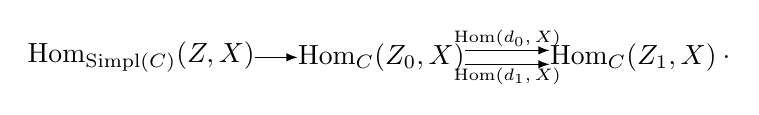
\begin{tikzpicture}[baseline=(b.base),>=latex]
    \node[inner sep=0pt] (a) at (0,0)
      {$\operatorname{Hom}_{\operatorname{Simpl}(C)}(Z,X)$};
    \node[inner sep=0pt] (b) at (3.05,0)
      {$\operatorname{Hom}_{C}(Z_0,X)$};
    \node[inner sep=0pt] (c) at (6.25,0)
      {$\operatorname{Hom}_{C}(Z_1,X)$};
    \draw[->] (a) -- (b);
    \draw[->]
      ([yshift=2.5bp]b.east) --
      node[above,inner sep=1bp,font=\fontsize{5.7}{6.4}\selectfont]
        {$\operatorname{Hom}(d_0,X)$}
      ([yshift=2.5bp]c.west);
    \draw[->]
      ([yshift=-2.5bp]b.east) --
      node[below,inner sep=1bp,font=\fontsize{5.7}{6.4}\selectfont]
        {$\operatorname{Hom}(d_1,X)$}
      ([yshift=-2.5bp]c.west);
    \node[anchor=west,inner sep=0pt,outer sep=0pt] at ([xshift=2bp]c.east) {.};
  \end{tikzpicture}%
}

% END ASSEMBLED SOURCE: tex/common/eq1.tex


% BEGIN ASSEMBLED SOURCE: tex/common/hom1.tex
% Native-TeX homotopy diagrams from LNM 239, physical p.21 / printed p.3.
\newcommand{\IllusieHomotopyTriangle}{%
  \begin{center}
  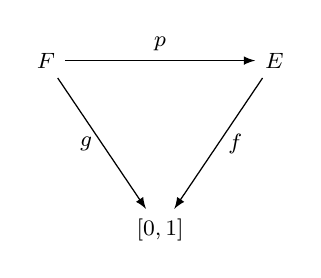
\begin{tikzpicture}[
    >=latex,
    line width=0.45pt,
    every node/.style={font=\rmfamily\fontsize{8}{9}\selectfont}
  ]
    \node (F) at (-1.45,1.0) {$F$};
    \node (E) at (1.45,1.0) {$E$};
    \node (I) at (0,-1.15) {$[0,1]$};
    \draw[->] (F) -- node[above] {$p$} (E);
    \draw[->] (F) -- node[left] {$g$} (I);
    \draw[->] (E) -- node[right] {$f$} (I);
  \end{tikzpicture}
  \end{center}%
}

\newcommand{\IllusieHomotopySquare}{%
  \begin{center}
  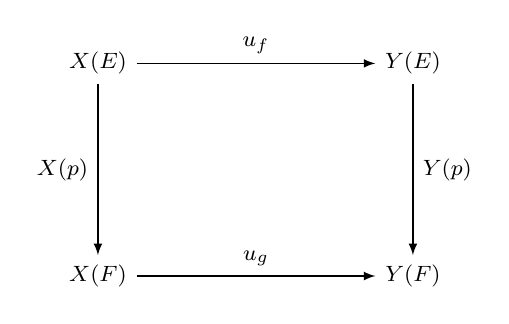
\begin{tikzpicture}[
    >=latex,
    line width=0.45pt,
    every node/.style={font=\rmfamily\fontsize{8}{9}\selectfont}
  ]
    \node (XE) at (-2.0,1.35) {$X(E)$};
    \node (YE) at (2.0,1.35) {$Y(E)$};
    \node (XF) at (-2.0,-1.35) {$X(F)$};
    \node (YF) at (2.0,-1.35) {$Y(F)$};
    \draw[->] (XE) -- node[above] {$u_f$} (YE);
    \draw[->] (XE) -- node[left] {$X(p)$} (XF);
    \draw[->] (YE) -- node[right] {$Y(p)$} (YF);
    \draw[->] (XF) -- node[above] {$u_g$} (YF);
  \end{tikzpicture}
  \end{center}%
}

% END ASSEMBLED SOURCE: tex/common/hom1.tex


% BEGIN ASSEMBLED SOURCE: tex/common/hom2.tex
% Native-TeX pullback square from LNM 239, physical p.58 / printed p.40.
\newcommand{\IllusieHomsPullbackSquare}{%
  \begin{center}
  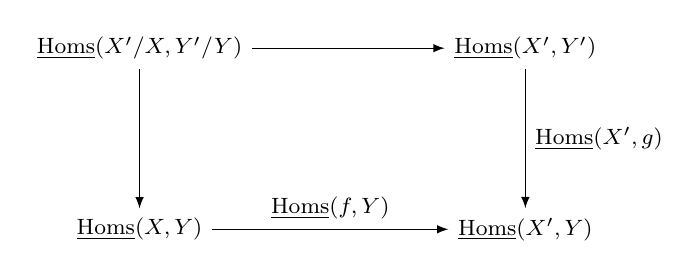
\begin{tikzpicture}[
    >=latex,
    line width=0.42pt,
    every node/.style={font=\rmfamily\fontsize{8.15}{8.8}\selectfont}
  ]
    \node (TL) at (-2.45, 1.15)
      {$\underline{\operatorname{Homs}}(X'/X,Y'/Y)$};
    \node (TR) at ( 2.45, 1.15)
      {$\underline{\operatorname{Homs}}(X',Y')$};
    \node (BL) at (-2.45,-1.15)
      {$\underline{\operatorname{Homs}}(X,Y)$};
    \node (BR) at ( 2.45,-1.15)
      {$\underline{\operatorname{Homs}}(X',Y)$};
    \draw[->] (TL) -- (TR);
    \draw[->] (TL) -- (BL);
    \draw[->] (TR) -- node[right]
      {$\underline{\operatorname{Homs}}(X',g)$} (BR);
    \draw[->] (BL) -- node[above]
      {$\underline{\operatorname{Homs}}(f,Y)$} (BR);
  \end{tikzpicture}
  \end{center}%
}

% END ASSEMBLED SOURCE: tex/common/hom2.tex


% BEGIN ASSEMBLED SOURCE: tex/common/hom3.tex
% Native-TeX mapping-cylinder diagrams from LNM 239, physical p.62 / printed p.44.
\newcommand{\IllusieMappingCylinderTriangle}{%
  \begin{center}
  \begin{tikzpicture}[
    >=latex,
    line width=0.44pt,
    every node/.style={font=\rmfamily\fontsize{8.4}{9}\selectfont}
  ]
    \node (Yp) at (0,1.18) {$Y'$};
    \node (X)  at (-1.65,-0.92) {$X$};
    \node (Y)  at ( 1.65,-0.92) {$Y$};
    \draw[right hook->] (X) -- node[left] {$i$} (Yp);
    \draw[->] (Yp) -- node[right] {$p$} (Y);
    \draw[->] (X) -- node[above] {$f$} (Y);
    \node at (2.35,-0.92) {,};
  \end{tikzpicture}
  \end{center}%
}

\newcommand{\IllusieMappingCylinderPushout}{%
  \begin{center}
  \begin{tikzpicture}[
    >=latex,
    line width=0.44pt,
    every node/.style={font=\rmfamily\fontsize{8.4}{9}\selectfont}
  ]
    \node (DX) at (-2.00, 1.08) {$\Delta(1)\times X$};
    \node (Yp) at ( 2.00, 1.08) {$Y'$};
    \node (X)  at (-2.00,-1.08) {$X$};
    \node (Y)  at ( 2.00,-1.08) {$Y$};
    \draw[->] (DX) -- node[above] {$f'$} (Yp);
    \draw[right hook->] (X) -- node[left] {$d^1$} (DX);
    \draw[right hook->] (Y) -- node[right] {$j$} (Yp);
    \draw[->] (X) -- node[above] {$f$} (Y);
    \node at (2.70,-1.08) {,};
  \end{tikzpicture}
  \end{center}%
}

% END ASSEMBLED SOURCE: tex/common/hom3.tex


% BEGIN ASSEMBLED SOURCE: tex/common/hom4.tex
% Native fraction-calculus diagrams from LNM 239, physical p.63 / printed p.45.
\newcommand{\IllusieFractionProofSource}{%
  \begin{center}
  \begin{tikzpicture}[
    >=latex,line width=0.44pt,
    every node/.style={font=\rmfamily\fontsize{8.4}{9}\selectfont,inner sep=1pt}
  ]
    \node (Xp) at (0,1.15) {$X'$};
    \node (X)  at (0,0) {$X$};
    \node (Y)  at (2.25,0) {$Y$};
    \draw[->] (X) -- node[left] {$s$} (Xp);
    \draw[->] (X) -- node[above] {$u$} (Y);
    \node at (2.85,0) {,};
  \end{tikzpicture}
  \end{center}%
}

\newcommand{\IllusieFractionProofPushout}{%
  \begin{center}
  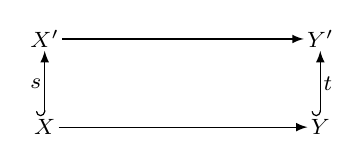
\begin{tikzpicture}[
    >=latex,line width=0.44pt,
    every node/.style={font=\rmfamily\fontsize{8.4}{9}\selectfont,inner sep=1pt}
  ]
    \node (Xp) at (-1.75,1.12) {$X'$};
    \node (Yp) at ( 1.75,1.12) {$Y'$};
    \node (X)  at (-1.75,0) {$X$};
    \node (Y)  at ( 1.75,0) {$Y$};
    \draw[->] (Xp) -- (Yp);
    \draw[right hook->] (X) -- node[left] {$s$} (Xp);
    \draw[right hook->] (Y) -- node[right] {$t$} (Yp);
    \draw[->] (X) -- (Y);
  \end{tikzpicture}
  \end{center}%
}

\newcommand{\IllusieFractionProofParallel}{%
  \begin{center}
  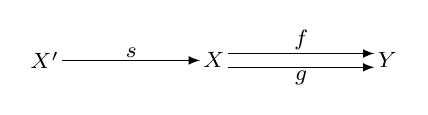
\begin{tikzpicture}[
    >=latex,line width=0.44pt,
    every node/.style={font=\rmfamily\fontsize{8.4}{9}\selectfont,inner sep=1pt}
  ]
    \node (Xp) at (-2.15,0) {$X'$};
    \node (X)  at (0,0) {$X$};
    \node (Y)  at (2.20,0) {$Y$};
    \draw[->] (Xp) -- node[above] {$s$} (X);
    \draw[->] ([yshift=2.5pt]X.east) -- node[above] {$f$} ([yshift=2.5pt]Y.west);
    \draw[->] ([yshift=-2.5pt]X.east) -- node[below] {$g$} ([yshift=-2.5pt]Y.west);
  \end{tikzpicture}
  \end{center}%
}

% END ASSEMBLED SOURCE: tex/common/hom4.tex


% BEGIN ASSEMBLED SOURCE: tex/common/hom5.tex
% Native pushout diagram from LNM 239, physical p.64 / printed p.46.
\newcommand{\IllusieCompositeHomotopyPushouts}{%
  \begin{center}
  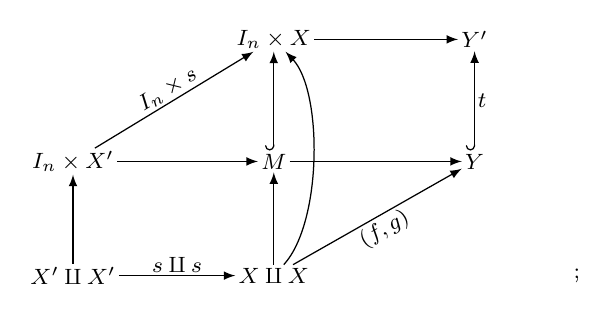
\begin{tikzpicture}[
    >=latex,x=1cm,y=1cm,line width=0.45pt,
    every node/.style={font=\rmfamily\fontsize{8}{9}\selectfont,inner sep=1pt}
  ]
    \node (IX)  at (0,1.55) {$I_n\times X$};
    \node (Yp)  at (2.55,1.55) {$Y'$};
    \node (IXp) at (-2.55,0) {$I_n\times X'$};
    \node (M)   at (0,0) {$M$};
    \node (Y)   at (2.55,0) {$Y$};
    \node (XXp) at (-2.55,-1.45) {$X'\amalg X'$};
    \node (XX)  at (0,-1.45) {$X\amalg X$};

    \draw[->] (IX) -- (Yp);
    \draw[right hook->] (Y) -- node[right] {$t$} (Yp);
    \draw[->] (IXp) -- (M);
    \draw[->] (M) -- (Y);
    \draw[->] (XXp) -- (IXp);
    \draw[->] (XXp) -- node[above] {$s\amalg s$} (XX);
    \draw[->] (XX) -- (M);
    \draw[->] (IXp) -- node[above,sloped] {$I_n\times s$} (IX);
    \draw[right hook->] (M) -- (IX);
    \draw[->] (XX) .. controls (0.62,-0.77) and (0.62,0.90) .. (IX);
    \draw[->] (XX) -- node[below,sloped] {$(f,g)$} (Y);
    \node at (3.85,-1.45) {$;$};
  \end{tikzpicture}
  \end{center}%
}

% END ASSEMBLED SOURCE: tex/common/hom5.tex


% BEGIN ASSEMBLED SOURCE: tex/common/hom6.tex
% Native lifting diagrams from LNM 239, physical p.65 / printed p.47.
\newcommand{\IllusieLocalLiftingSquare}{%
  \begin{center}
  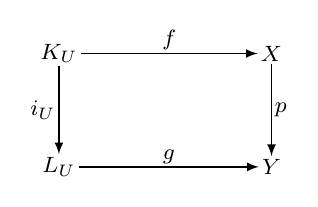
\begin{tikzpicture}[
    >=latex,x=1cm,y=1cm,line width=0.45pt,
    every node/.style={font=\rmfamily\fontsize{8}{9}\selectfont,inner sep=1pt}
  ]
    \node (KU) at (-1.35,0.72) {$K_U$};
    \node (X)  at (1.35,0.72) {$X$};
    \node (LU) at (-1.35,-0.72) {$L_U$};
    \node (Y)  at (1.35,-0.72) {$Y$};
    \draw[->] (KU) -- node[above] {$f$} (X);
    \draw[->] (KU) -- node[left] {$i_U$} (LU);
    \draw[->] (X) -- node[right] {$p$} (Y);
    \draw[->] (LU) -- node[above] {$g$} (Y);
  \end{tikzpicture}
  \end{center}%
}

\newcommand{\IllusieLocalLiftDiagram}{%
  \begin{center}
  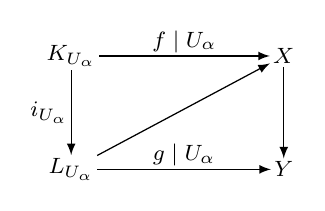
\begin{tikzpicture}[
    >=latex,x=1cm,y=1cm,line width=0.45pt,
    every node/.style={font=\rmfamily\fontsize{8}{9}\selectfont,inner sep=1pt}
  ]
    \node (KU) at (-1.35,0.72) {$K_{U_\alpha}$};
    \node (X)  at (1.35,0.72) {$X$};
    \node (LU) at (-1.35,-0.72) {$L_{U_\alpha}$};
    \node (Y)  at (1.35,-0.72) {$Y$};
    \draw[->] (KU) -- node[above] {$f\mid U_\alpha$} (X);
    \draw[->] (KU) -- node[left] {$i_{U_\alpha}$} (LU);
    \draw[->] (X) -- (Y);
    \draw[->] (LU) -- node[above] {$g\mid U_\alpha$} (Y);
    \draw[->] (LU) -- (X);
  \end{tikzpicture}
  \end{center}%
}

% END ASSEMBLED SOURCE: tex/common/hom6.tex


% BEGIN ASSEMBLED SOURCE: tex/common/tri1.tex
% Native-TeX transitivity triangle from LNM 239, physical p.12 / Roman X.
\newcommand{\IllusieTransitivityTriangle}{%
  \begin{center}
  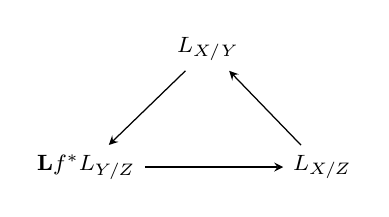
\begin{tikzpicture}[
    >=stealth,
    line width=0.45pt,
    every node/.style={font=\rmfamily\fontsize{8.15}{9}\selectfont}
  ]
    \node (xy) at (0,1.05) {$L_{X/Y}$};
    \node (fyz) at (-1.55,-0.45) {$\mathbf L f^{*}L_{Y/Z}$};
    \node (xz) at (1.45,-0.45) {$L_{X/Z}$};
    \draw[->] (xy) -- (fyz);
    \draw[->] (fyz) -- (xz);
    \draw[->] (xz) -- (xy);
  \end{tikzpicture}
  \end{center}%
}

% END ASSEMBLED SOURCE: tex/common/tri1.tex


% BEGIN ASSEMBLED SOURCE: tex/common/guide1.tex
% Native chapter-dependency guide from LNM 239 physical p.17 / Roman XV.
\newcommand{\IllusieChapterGuide}{%
  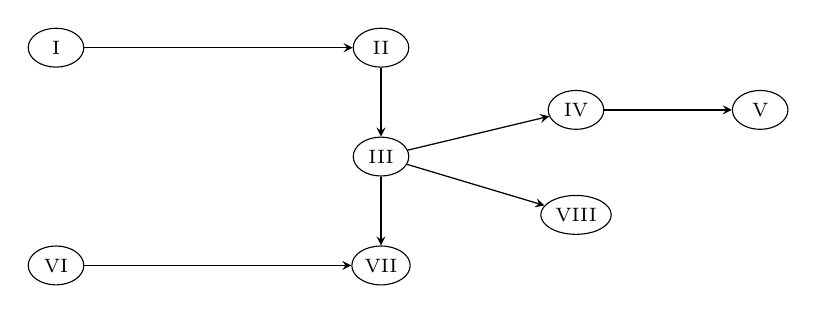
\begin{tikzpicture}[
    x=39bp,y=28bp,>=stealth,
    guide node/.style={draw,ellipse,minimum width=20bp,minimum height=14bp,
      inner sep=1.5bp,font=\fontsize{7}{7}\selectfont},
    guide arrow/.style={->,line width=0.45pt}
  ]
    \node[guide node] (I) at (0,2.8) {I};
    \node[guide node] (II) at (3,2.8) {II};
    \node[guide node] (III) at (3,1.4) {III};
    \node[guide node] (IV) at (4.8,2.0) {IV};
    \node[guide node] (V) at (6.5,2.0) {V};
    \node[guide node] (VIII) at (4.8,0.65) {VIII};
    \node[guide node] (VII) at (3,0) {VII};
    \node[guide node] (VI) at (0,0) {VI};
    \draw[guide arrow] (I) -- (II);
    \draw[guide arrow] (II) -- (III);
    \draw[guide arrow] (III) -- (IV);
    \draw[guide arrow] (IV) -- (V);
    \draw[guide arrow] (III) -- (VIII);
    \draw[guide arrow] (III) -- (VII);
    \draw[guide arrow] (VI) -- (VII);
  \end{tikzpicture}%
}

% END ASSEMBLED SOURCE: tex/common/guide1.tex


% BEGIN ASSEMBLED SOURCE: tex/common/assoc1.tex
% Native-TeX associativity/coassociativity squares from LNM 239,
% physical p.26 / printed p.8, formula (1.2.2.3).
\newcommand{\IllusieAssociativitySquares}{%
  \begin{center}
  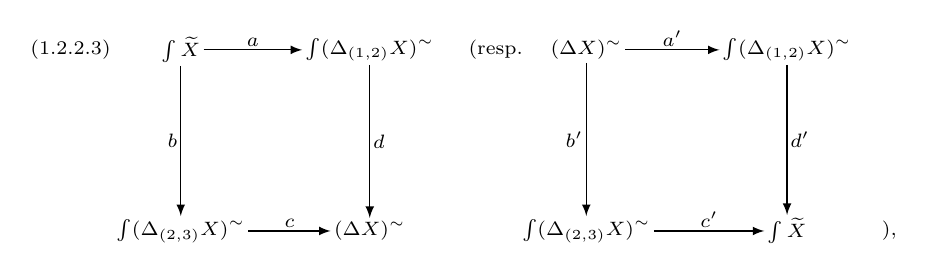
\begin{tikzpicture}[
    >=latex,
    x=1cm,
    y=1cm,
    line width=0.45pt,
    every node/.style={font=\rmfamily\fontsize{7.2}{8}\selectfont,inner sep=1pt}
  ]
    \node at (-6.35,1.15) {(1.2.2.3)};

    \node (LTL) at (-4.95,1.15) {$\int\widetilde X$};
    \node (LTR) at (-2.55,1.15) {$\int(\Delta_{(1,2)}X)^{\sim}$};
    \node (LBL) at (-4.95,-1.15) {$\int(\Delta_{(2,3)}X)^{\sim}$};
    \node (LBR) at (-2.55,-1.15) {$(\Delta X)^{\sim}$};
    \draw[->] (LTL) -- node[above] {$a$} (LTR);
    \draw[->] (LTL) -- node[left] {$b$} (LBL);
    \draw[->] (LBL) -- node[above] {$c$} (LBR);
    \draw[->] (LTR) -- node[right] {$d$} (LBR);

    \node at (-0.95,1.15) {(resp.};
    \node (RTL) at (0.20,1.15) {$(\Delta X)^{\sim}$};
    \node (RTR) at (2.75,1.15) {$\int(\Delta_{(1,2)}X)^{\sim}$};
    \node (RBL) at (0.20,-1.15) {$\int(\Delta_{(2,3)}X)^{\sim}$};
    \node (RBR) at (2.75,-1.15) {$\int\widetilde X$};
    \draw[->] (RTL) -- node[above] {$a'$} (RTR);
    \draw[->] (RTL) -- node[left] {$b'$} (RBL);
    \draw[->] (RBL) -- node[above] {$c'$} (RBR);
    \draw[->] (RTR) -- node[right] {$d'$} (RBR);
    \node at (4.05,-1.15) {),};
  \end{tikzpicture}
  \end{center}%
}

% END ASSEMBLED SOURCE: tex/common/assoc1.tex


% BEGIN ASSEMBLED SOURCE: tex/common/dold1.tex
% Native-TeX factorization square from LNM 239,
% physical p.27 / printed p.9, section 1.3.1.
\newcommand{\IllusieDoldPuppeSquare}{%
  \begin{center}
  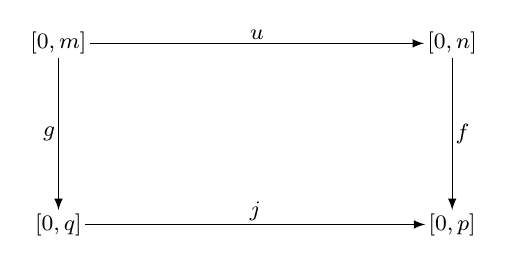
\begin{tikzpicture}[
    >=latex,
    x=1cm,
    y=1cm,
    line width=0.45pt,
    every node/.style={font=\rmfamily\fontsize{8}{9}\selectfont,inner sep=1pt}
  ]
    \node (TL) at (-2.5,1.15) {$[0,m]$};
    \node (TR) at (2.5,1.15) {$[0,n]$};
    \node (BL) at (-2.5,-1.15) {$[0,q]$};
    \node (BR) at (2.5,-1.15) {$[0,p]$};
    \draw[->] (TL) -- node[above] {$u$} (TR);
    \draw[->] (TL) -- node[left] {$g$} (BL);
    \draw[->] (TR) -- node[right] {$f$} (BR);
    \draw[->] (BL) -- node[above] {$j$} (BR);
  \end{tikzpicture}
  \end{center}%
}

% END ASSEMBLED SOURCE: tex/common/dold1.tex


% BEGIN ASSEMBLED SOURCE: tex/common/dold2.tex
% Native normal/degenerate restriction diagram from LNM 239,
% physical p.29 / printed p.11, section 1.3.5.
\newcommand{\IllusieNormalDegenerateDiagram}{%
  \begin{center}
  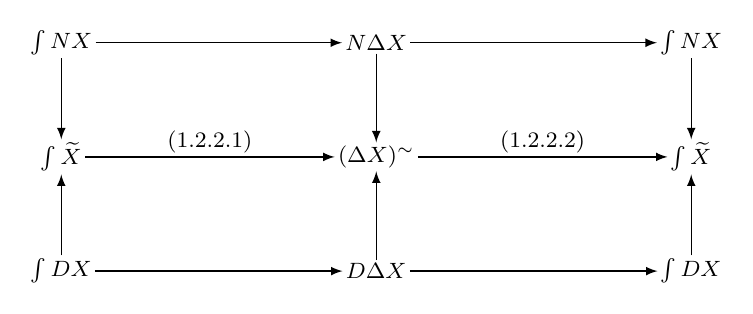
\begin{tikzpicture}[
    >=latex,
    x=1cm,
    y=1cm,
    line width=0.45pt,
    every node/.style={font=\rmfamily\fontsize{8}{9}\selectfont,inner sep=1pt}
  ]
    \node (TL) at (-4.0,1.45) {$\int NX$};
    \node (TC) at (0,1.45) {$N\Delta X$};
    \node (TR) at (4.0,1.45) {$\int NX$};
    \node (ML) at (-4.0,0) {$\int\widetilde X$};
    \node (MC) at (0,0) {$(\Delta X)^{\sim}$};
    \node (MR) at (4.0,0) {$\int\widetilde X$};
    \node (BL) at (-4.0,-1.45) {$\int DX$};
    \node (BC) at (0,-1.45) {$D\Delta X$};
    \node (BR) at (4.0,-1.45) {$\int DX$};

    \draw[->] (TL) -- (TC);
    \draw[->] (TC) -- (TR);
    \draw[->] (ML) -- node[above] {(1.2.2.1)} (MC);
    \draw[->] (MC) -- node[above] {(1.2.2.2)} (MR);
    \draw[->] (BL) -- (BC);
    \draw[->] (BC) -- (BR);
    \draw[->] (TL) -- (ML);
    \draw[->] (TC) -- (MC);
    \draw[->] (TR) -- (MR);
    \draw[->] (BL) -- (ML);
    \draw[->] (BC) -- (MC);
    \draw[->] (BR) -- (MR);
  \end{tikzpicture}
  \end{center}%
}

% END ASSEMBLED SOURCE: tex/common/dold2.tex


% BEGIN ASSEMBLED SOURCE: tex/common/fractions1.tex
% Native right/left calculus-of-fractions diagrams from LNM 239,
% physical p.30 / printed p.12, section 1.4.2.
\newcommand{\IllusieRightFractionFrThreeSource}{%
  \begin{center}
  \begin{tikzpicture}[
    >=latex,x=1cm,y=1cm,line width=0.45pt,
    every node/.style={font=\rmfamily\fontsize{8}{9}\selectfont,inner sep=1pt}
  ]
    \node (X) at (-1.7,0) {$X$};
    \node (Y) at (1.7,0) {$Y$};
    \node (Yp) at (1.7,1.35) {$Y'$};
    \draw[->] (X) -- node[above] {$u$} (Y);
    \draw[->] (Yp) -- node[right] {$t$} (Y);
  \end{tikzpicture}
  \end{center}%
}

\newcommand{\IllusieRightFractionFrThreeCompletion}{%
  \begin{center}
  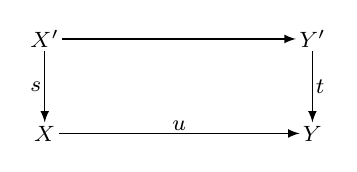
\begin{tikzpicture}[
    >=latex,x=1cm,y=1cm,line width=0.45pt,
    every node/.style={font=\rmfamily\fontsize{8}{9}\selectfont,inner sep=1pt}
  ]
    \node (Xp) at (-1.7,1.2) {$X'$};
    \node (Yp) at (1.7,1.2) {$Y'$};
    \node (X) at (-1.7,0) {$X$};
    \node (Y) at (1.7,0) {$Y$};
    \draw[->] (Xp) -- (Yp);
    \draw[->] (Xp) -- node[left] {$s$} (X);
    \draw[->] (Yp) -- node[right] {$t$} (Y);
    \draw[->] (X) -- node[above] {$u$} (Y);
  \end{tikzpicture}
  \end{center}%
}

\newcommand{\IllusieRightFractionFrFourSource}{%
  \begin{center}
  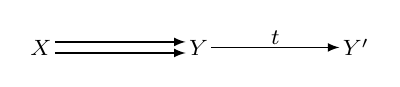
\begin{tikzpicture}[
    >=latex,x=1cm,y=1cm,line width=0.45pt,
    every node/.style={font=\rmfamily\fontsize{8}{9}\selectfont,inner sep=1pt}
  ]
    \node (X) at (-2.0,0) {$X$};
    \node (Y) at (0,0) {$Y$};
    \node (Yp) at (2.0,0) {$Y'$};
    \draw[->] ([yshift=2pt]X.east) -- ([yshift=2pt]Y.west);
    \draw[->] ([yshift=-2pt]X.east) -- ([yshift=-2pt]Y.west);
    \draw[->] (Y) -- node[above] {$t$} (Yp);
  \end{tikzpicture}
  \end{center}%
}

\newcommand{\IllusieRightFractionFrFourCompletion}{%
  \begin{center}
  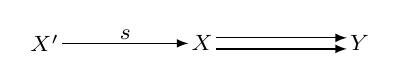
\begin{tikzpicture}[
    >=latex,x=1cm,y=1cm,line width=0.45pt,
    every node/.style={font=\rmfamily\fontsize{8}{9}\selectfont,inner sep=1pt}
  ]
    \node (Xp) at (-2.0,0) {$X'$};
    \node (X) at (0,0) {$X$};
    \node (Y) at (2.0,0) {$Y$};
    \draw[->] (Xp) -- node[above] {$s$} (X);
    \draw[->] ([yshift=2pt]X.east) -- ([yshift=2pt]Y.west);
    \draw[->] ([yshift=-2pt]X.east) -- ([yshift=-2pt]Y.west);
  \end{tikzpicture}
  \end{center}%
}

\newcommand{\IllusieLeftFractionFrThreeSource}{%
  \begin{center}
  \begin{tikzpicture}[
    >=latex,x=1cm,y=1cm,line width=0.45pt,
    every node/.style={font=\rmfamily\fontsize{8}{9}\selectfont,inner sep=1pt}
  ]
    \node (X) at (-1.5,0.8) {$X$};
    \node (Y) at (1.5,0.8) {$Y$};
    \node (Xp) at (-1.5,-0.65) {$X'$};
    \draw[->] (X) -- node[above] {$u$} (Y);
    \draw[->] (X) -- node[left] {$s$} (Xp);
  \end{tikzpicture}
  \end{center}%
}

\newcommand{\IllusieLeftFractionFrThreeCompletion}{%
  \begin{center}
  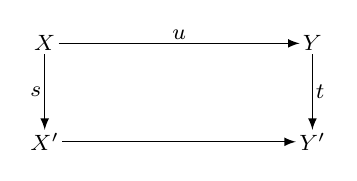
\begin{tikzpicture}[
    >=latex,x=1cm,y=1cm,line width=0.45pt,
    every node/.style={font=\rmfamily\fontsize{8}{9}\selectfont,inner sep=1pt}
  ]
    \node (X) at (-1.7,1.25) {$X$};
    \node (Y) at (1.7,1.25) {$Y$};
    \node (Xp) at (-1.7,0) {$X'$};
    \node (Yp) at (1.7,0) {$Y'$};
    \draw[->] (X) -- node[above] {$u$} (Y);
    \draw[->] (X) -- node[left] {$s$} (Xp);
    \draw[->] (Y) -- node[right] {$t$} (Yp);
    \draw[->] (Xp) -- (Yp);
  \end{tikzpicture}
  \end{center}%
}

\newcommand{\IllusieLeftFractionFrFourSource}{%
  \begin{center}
  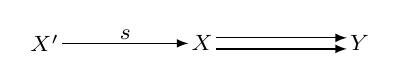
\begin{tikzpicture}[
    >=latex,x=1cm,y=1cm,line width=0.45pt,
    every node/.style={font=\rmfamily\fontsize{8}{9}\selectfont,inner sep=1pt}
  ]
    \node (Xp) at (-2.0,0) {$X'$};
    \node (X) at (0,0) {$X$};
    \node (Y) at (2.0,0) {$Y$};
    \draw[->] (Xp) -- node[above] {$s$} (X);
    \draw[->] ([yshift=2pt]X.east) -- ([yshift=2pt]Y.west);
    \draw[->] ([yshift=-2pt]X.east) -- ([yshift=-2pt]Y.west);
  \end{tikzpicture}
  \end{center}%
}

\newcommand{\IllusieLeftFractionFrFourCompletion}{%
  \begin{center}
  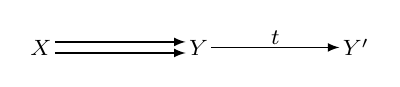
\begin{tikzpicture}[
    >=latex,x=1cm,y=1cm,line width=0.45pt,
    every node/.style={font=\rmfamily\fontsize{8}{9}\selectfont,inner sep=1pt}
  ]
    \node (X) at (-2.0,0) {$X$};
    \node (Y) at (0,0) {$Y$};
    \node (Yp) at (2.0,0) {$Y'$};
    \draw[->] ([yshift=2pt]X.east) -- ([yshift=2pt]Y.west);
    \draw[->] ([yshift=-2pt]X.east) -- ([yshift=-2pt]Y.west);
    \draw[->] (Y) -- node[above] {$t$} (Yp);
  \end{tikzpicture}
  \end{center}%
}

% END ASSEMBLED SOURCE: tex/common/fractions1.tex


% BEGIN ASSEMBLED SOURCE: tex/common/derived1.tex
% Native 2-cell diagram from LNM 239, physical p.32 / printed p.14,
% section 1.4.4. The 2-cell v has target F, as does u_F.
\newcommand{\IllusieLeftDerivedUniversalTriangle}{%
  \begin{center}
  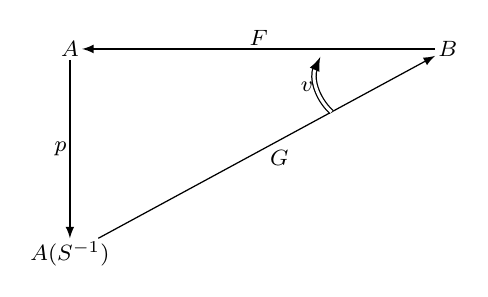
\begin{tikzpicture}[
    >=latex,x=1cm,y=1cm,line width=0.45pt,
    every node/.style={font=\rmfamily\fontsize{8}{9}\selectfont,inner sep=1pt}
  ]
    \node (A) at (-2.4,1.5) {$A$};
    \node (AS) at (-2.4,-1.1) {$A(S^{-1})$};
    \node (B) at (2.4,1.5) {$B$};
    \draw[->] (B) -- node[above] {$F$} (A);
    \draw[->] (A) -- node[left] {$p$} (AS);
    \draw[->] (AS) -- node[below right] {$G$} (B);
    \draw[double distance=1.1pt,->]
      (0.92,0.70) to[bend left=35] node[left] {$v$} (0.78,1.40);
  \end{tikzpicture}
  \end{center}%
}

% END ASSEMBLED SOURCE: tex/common/derived1.tex


% BEGIN ASSEMBLED SOURCE: tex/common/derived2.tex
% Native comparison grid from LNM 239, physical p.33 / printed p.15,
% section 1.4.5. Horizontal arrows are N and K; vertical arrows localize.
\newcommand{\IllusieDerivedComparisonGrid}{%
  \begin{center}
  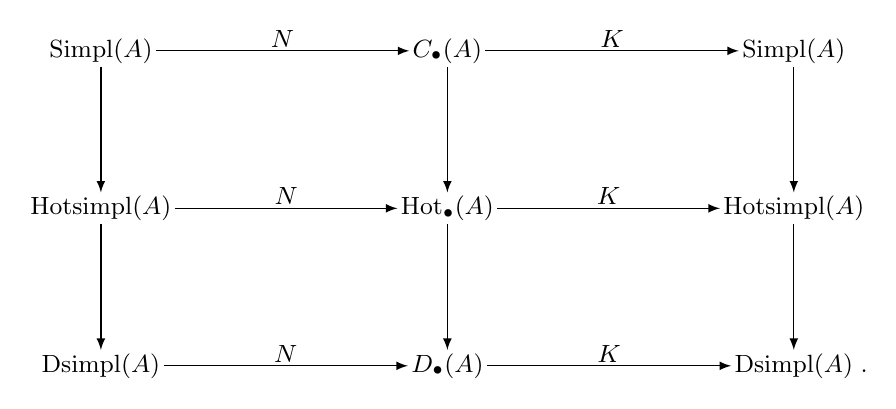
\begin{tikzpicture}[
    >=latex,x=1cm,y=1cm,line width=0.45pt,
    every node/.style={font=\rmfamily\fontsize{9}{10}\selectfont,inner sep=1pt}
  ]
    \node (s0) at (-4.4,2) {$\operatorname{Simpl}(A)$};
    \node (c0) at (0,2) {$C_{\bullet}(A)$};
    \node (s1) at (4.4,2) {$\operatorname{Simpl}(A)$};
    \node (hs0) at (-4.4,0) {$\operatorname{Hotsimpl}(A)$};
    \node (hc0) at (0,0) {$\operatorname{Hot}_{\bullet}(A)$};
    \node (hs1) at (4.4,0) {$\operatorname{Hotsimpl}(A)$};
    \node (ds0) at (-4.4,-2) {$\operatorname{Dsimpl}(A)$};
    \node (dc0) at (0,-2) {$D_{\bullet}(A)$};
    \node (ds1) at (4.4,-2) {$\operatorname{Dsimpl}(A)$};

    \draw[->] (s0) -- node[above] {$N$} (c0);
    \draw[->] (c0) -- node[above] {$K$} (s1);
    \draw[->] (hs0) -- node[above] {$N$} (hc0);
    \draw[->] (hc0) -- node[above] {$K$} (hs1);
    \draw[->] (ds0) -- node[above] {$N$} (dc0);
    \draw[->] (dc0) -- node[above] {$K$} (ds1);

    \draw[->] (s0) -- (hs0);
    \draw[->] (c0) -- (hc0);
    \draw[->] (s1) -- (hs1);
    \draw[->] (hs0) -- (ds0);
    \draw[->] (hc0) -- (dc0);
    \draw[->] (hs1) -- (ds1);
    \node[anchor=base west,inner sep=0pt,outer sep=0pt] at ([xshift=1.5pt]ds1.base east) {.};
  \end{tikzpicture}
  \end{center}%
}

% END ASSEMBLED SOURCE: tex/common/derived2.tex


% BEGIN ASSEMBLED SOURCE: tex/common/local2.tex
% Native-TeX diagrams for Lemma 2.2.6, LNM 239 physical p.47 / printed p.29.
\newcommand{\IllusieLocalObjectSquare}{%
  \begin{center}
  \begin{tikzpicture}[
    >=latex,
    line width=0.45pt,
    every node/.style={font=\rmfamily\fontsize{9.3}{10.4}\selectfont}
  ]
    \node (Ei) at (-2.0,1.55) {$E_i$};
    \node (Fi) at ( 2.0,1.55) {$F_i$};
    \node (EU) at (-2.0,-1.55) {$E(U)$};
    \node (FU) at ( 2.0,-1.55) {$F(U)$};
    \draw[->] (Ei) -- node[above] {$u_i$} (Fi);
    \draw[->] (Ei) -- (EU);
    \draw[->] (Fi) -- (FU);
    \draw[->] (EU) -- node[above] {$u(U)$} (FU);
    \node at (2.55,-1.55) {,};
  \end{tikzpicture}
  \end{center}%
}

\newcommand{\IllusieLocalRestrictionSquare}{%
  \begin{center}
  \begin{tikzpicture}[
    >=latex,
    line width=0.45pt,
    every node/.style={font=\rmfamily\fontsize{9.3}{10.4}\selectfont}
  ]
    \node (Ei) at (-2.0,1.55) {$E_i$};
    \node (Fi) at ( 2.0,1.55) {$F_i$};
    \node (EU) at (-2.0,-1.55) {$E\vert U$};
    \node (FU) at ( 2.0,-1.55) {$F\vert U$};
    \draw[->] (Ei) -- node[above] {$u_i$} (Fi);
    \draw[->] (Ei) -- (EU);
    \draw[->] (Fi) -- (FU);
    \draw (EU) -- node[above] {$u\vert U$} (FU);
    \node at (2.55,-1.55) {,};
  \end{tikzpicture}
  \end{center}%
}

\newcommand{\IllusieLocalMorphismTriangle}{%
  \begin{center}
  \begin{tikzpicture}[
    >=latex,
    line width=0.45pt,
    every node/.style={font=\rmfamily\fontsize{9.3}{10.4}\selectfont}
  ]
    \node (ui) at (-1.75,1.25) {$u_i$};
    \node (uj) at ( 1.75,1.25) {$u_j$};
    \node (u)  at (0,-1.25) {$u(U)$};
    \draw[->] (ui) -- node[above] {$f$} (uj);
    \draw[->] (ui) -- node[left] {$i$} (u);
    \draw[->] (uj) -- node[right] {$j$} (u);
    \node at (2.25,-1.25) {.};
  \end{tikzpicture}
  \end{center}%
}

% END ASSEMBLED SOURCE: tex/common/local2.tex


% BEGIN ASSEMBLED SOURCE: tex/common/local3.tex
% Native-TeX diagram for Lemma 2.2.6, LNM 239 physical p.48 / printed p.30.
\newcommand{\IllusieFinitePresentationCube}{%
  \begin{center}
  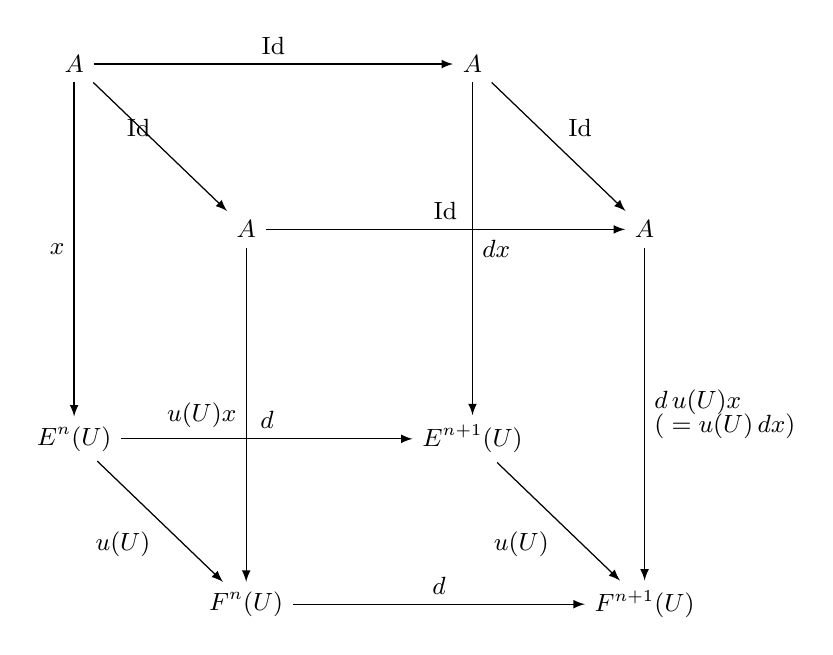
\begin{tikzpicture}[
    x=1.15cm,
    y=1.40cm,
    >=latex,
    line width=0.45pt,
    every node/.style={font=\rmfamily\fontsize{8.8}{9.8}\selectfont}
  ]
    \node (A0) at (-3.2, 2.6) {$A$};
    \node (A1) at ( 1.2, 2.6) {$A$};
    \node (B0) at (-1.3, 1.1) {$A$};
    \node (B1) at ( 3.1, 1.1) {$A$};
    \node (E0) at (-3.2,-0.8) {$E^n(U)$};
    \node (E1) at ( 1.2,-0.8) {$E^{n+1}(U)$};
    \node (F0) at (-1.3,-2.3) {$F^n(U)$};
    \node (F1) at ( 3.1,-2.3) {$F^{n+1}(U)$};
    \draw[->] (A0) -- node[above] {$\operatorname{Id}$} (A1);
    \draw[->] (A0) -- node[above left] {$\operatorname{Id}$} (B0);
    \draw[->] (A1) -- node[above right] {$\operatorname{Id}$} (B1);
    \draw[->] (B0) -- node[above] {$\operatorname{Id}$} (B1);
    \draw[->] (A0) -- node[left] {$x$} (E0);
    \draw[->] (A1) -- node[right] {$dx$} (E1);
    \draw[->] (B0) -- node[left] {$u(U)x$} (F0);
    \draw[->] (B1) -- node[right,align=left] {$d\,u(U)x$\\[-1pt]$({}=u(U)\,dx)$} (F1);
    \draw[->] (E0) -- node[above] {$d$} (E1);
    \draw[->] (F0) -- node[above] {$d$} (F1);
    \draw[->] (E0) -- node[below left] {$u(U)$} (F0);
    \draw[->] (E1) -- node[below left] {$u(U)$} (F1);
  \end{tikzpicture}
  \end{center}%
}

% END ASSEMBLED SOURCE: tex/common/local3.tex


% BEGIN ASSEMBLED SOURCE: tex/common/local4.tex
% Native-TeX diagram for Lemma 2.2.7, LNM 239 physical p.49 / printed p.31.
\newcommand{\IllusieExtensionLemmaTriangle}{%
  \begin{center}
  \begin{tikzpicture}[
    >=latex,
    line width=0.42pt,
    every node/.style={font=\rmfamily\fontsize{8.15}{9.2}\selectfont}
  ]
    \node (z0) at (-4.10, 1.15) {$0$};
    \node (up) at (-2.55, 1.15) {$u'$};
    \node (upp) at (-0.35, 1.15) {$u''_{\alpha}$};
    \node (va) at ( 1.95, 1.15) {$v_{\alpha}$};
    \node (z1) at ( 3.75, 1.15) {$0$};
    \node (ua) at (-1.20,-1.55) {$u(U_{\alpha})$};
    \draw[->] (z0) -- (up);
    \draw[->] (up) -- (upp);
    \draw[->] (upp) -- (va);
    \draw[->] (va) -- (z1);
    \draw[->] (up) -- node[below left] {$f\vert U_{\alpha}$} (ua);
    \draw[->] (upp) -- (ua);
    \node at (2.95,-1.10) {,};
  \end{tikzpicture}
  \end{center}%
}

% END ASSEMBLED SOURCE: tex/common/local4.tex


% BEGIN ASSEMBLED SOURCE: tex/common/local5.tex
% Native-TeX diagrams for Lemma 2.2.7, LNM 239 physical p.50 / printed p.32.
\newcommand{\IllusieRTSquare}{%
  \begin{center}
  \begin{tikzpicture}[>=latex,line width=0.42pt,every node/.style={font=\rmfamily\fontsize{8.15}{9.2}\selectfont}]
    \node (M)  at (-2.80, 1.15) {$M$};
    \node (ZE) at ( 1.75, 1.15) {$Z^{n+1}(E')$};
    \node (Fn) at (-2.80,-1.15) {$F'^{n}$};
    \node (ZF) at ( 1.75,-1.15) {$Z^{n+1}(F')$};
    \draw[->] (M) -- node[above] {$r$} (ZE);
    \draw[->] (M) -- node[left] {$t$} (Fn);
    \draw[->] (ZE) -- node[right] {$u'$} (ZF);
    \draw[->] (Fn) -- (ZF);
    \node at (3.35,-1.15) {.};
  \end{tikzpicture}
  \end{center}%
}

\newcommand{\IllusieCohomologyRectangle}{%
  \begin{center}
  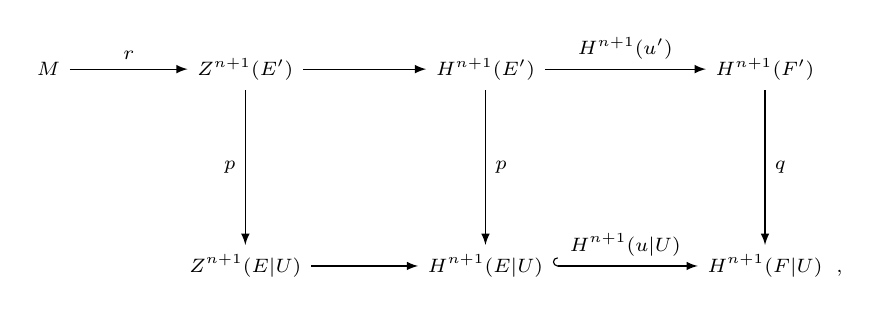
\begin{tikzpicture}[>=latex,line width=0.42pt,every node/.style={font=\rmfamily\fontsize{7.4}{8.5}\selectfont}]
    \node (M)   at (-5.65, 1.20) {$M$};
    \node (ZE)  at (-3.15, 1.20) {$Z^{n+1}(E')$};
    \node (HE)  at (-0.10, 1.20) {$H^{n+1}(E')$};
    \node (HF)  at ( 3.45, 1.20) {$H^{n+1}(F')$};
    \node (ZEU) at (-3.15,-1.30) {$Z^{n+1}(E\vert U)$};
    \node (HEU) at (-0.10,-1.30) {$H^{n+1}(E\vert U)$};
    \node (HFU) at ( 3.45,-1.30) {$H^{n+1}(F\vert U)$};
    \draw[->] (M) -- node[above] {$r$} (ZE);
    \draw[->] (ZE) -- (HE);
    \draw[->] (HE) -- node[above] {$H^{n+1}(u')$} (HF);
    \draw[->] (ZE) -- node[left] {$p$} (ZEU);
    \draw[->] (HE) -- node[right] {$p$} (HEU);
    \draw[->] (HF) -- node[right] {$q$} (HFU);
    \draw[->] (ZEU) -- (HEU);
    \draw[right hook->] (HEU) -- node[above] {$H^{n+1}(u\vert U)$} (HFU);
    \node[anchor=base west,inner sep=0pt,outer sep=0pt] at ([xshift=1.5pt]HFU.base east) {,};
  \end{tikzpicture}
  \end{center}%
}

\newcommand{\IllusieLocalizedSSquare}{%
  \begin{center}
  \begin{tikzpicture}[>=latex,line width=0.42pt,every node/.style={font=\rmfamily\fontsize{8.15}{9.2}\selectfont}]
    \node (M)   at (-2.80, 1.15) {$M$};
    \node (ZE)  at ( 1.75, 1.15) {$Z^{n+1}(E')$};
    \node (EnU) at (-2.80,-1.15) {$E^{n}\vert U$};
    \node (ZEU) at ( 1.75,-1.15) {$Z^{n+1}(E\vert U)$};
    \draw[->] (M) -- node[above] {$r$} (ZE);
    \draw[->] (M) -- node[left] {$s$} (EnU);
    \draw[->] (ZE) -- (ZEU);
    \draw[->] (EnU) -- (ZEU);
    \node[anchor=base west,inner sep=0pt,outer sep=0pt] at ([xshift=1.5pt]ZEU.base east) {.};
  \end{tikzpicture}
  \end{center}%
}

\newcommand{\IllusieTSQUquare}{%
  \begin{center}
  \begin{tikzpicture}[>=latex,line width=0.42pt,every node/.style={font=\rmfamily\fontsize{8.15}{9.2}\selectfont}]
    \node (M)   at (-2.80, 1.15) {$M$};
    \node (Fpn) at ( 1.75, 1.15) {$F'^{n}$};
    \node (EnU) at (-2.80,-1.15) {$E^{n}\vert U$};
    \node (FnU) at ( 1.75,-1.15) {$F^{n}\vert U$};
    \draw[->] (M) -- node[above] {$t$} (Fpn);
    \draw[->] (M) -- node[left] {$s$} (EnU);
    \draw[->] (Fpn) -- node[right] {$q$} (FnU);
    \draw[->] (EnU) -- node[above] {$u$} (FnU);
  \end{tikzpicture}
  \end{center}%
}

% END ASSEMBLED SOURCE: tex/common/local5.tex


% BEGIN ASSEMBLED SOURCE: tex/common/local6.tex
% Native-TeX diagrams for Lemma 2.2.7, LNM 239 physical p.51 / printed p.33.
\newcommand{\IllusieUDoublePrimeComplexMap}{%
  \begin{center}
  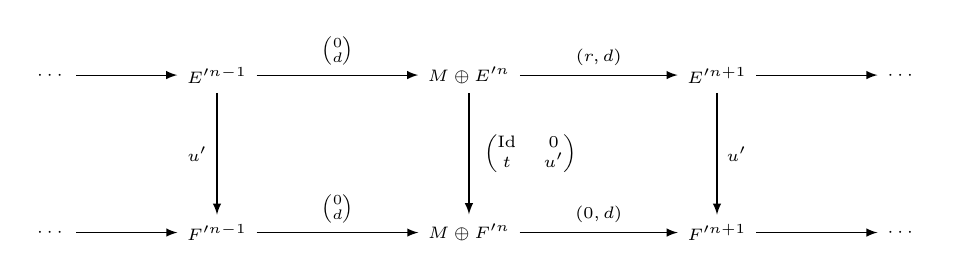
\begin{tikzpicture}[>=latex,line width=0.4pt,every node/.style={font=\rmfamily\fontsize{5.7}{6.2}\selectfont}]
    \node (ET0) at (-5.65, 1.00) {$\cdots$};
    \node (ET1) at (-3.55, 1.00) {$E'^{n-1}$};
    \node (ET2) at (-0.35, 1.00) {$M\oplus E'^n$};
    \node (ET3) at ( 2.80, 1.00) {$E'^{n+1}$};
    \node (ET4) at ( 5.15, 1.00) {$\cdots$};
    \node (FB0) at (-5.65,-1.00) {$\cdots$};
    \node (FB1) at (-3.55,-1.00) {$F'^{n-1}$};
    \node (FB2) at (-0.35,-1.00) {$M\oplus F'^n$};
    \node (FB3) at ( 2.80,-1.00) {$F'^{n+1}$};
    \node (FB4) at ( 5.15,-1.00) {$\cdots$};
    \draw[->] (ET0) -- (ET1); \draw[->] (ET1) -- node[above] {$\binom{0}{d}$} (ET2);
    \draw[->] (ET2) -- node[above] {$(r,d)$} (ET3); \draw[->] (ET3) -- (ET4);
    \draw[->] (FB0) -- (FB1); \draw[->] (FB1) -- node[above] {$\binom{0}{d}$} (FB2);
    \draw[->] (FB2) -- node[above] {$(0,d)$} (FB3); \draw[->] (FB3) -- (FB4);
    \draw[->] (ET1) -- node[left] {$u'$} (FB1);
    \draw[->] (ET2) -- node[right,xshift=2pt] {$\begin{pmatrix}\mathrm{Id}&0\\ t&u'\end{pmatrix}$} (FB2);
    \draw[->] (ET3) -- node[right] {$u'$} (FB3);
  \end{tikzpicture}
  \end{center}%
}

\newcommand{\IllusiePPrimeComplexMap}{%
  \begin{center}
  \begin{tikzpicture}[>=latex,line width=0.4pt,every node/.style={font=\rmfamily\fontsize{5.7}{6.2}\selectfont}]
    \node (ET0) at (-5.65, 1.00) {$\cdots$};
    \node (ET1) at (-3.55, 1.00) {$E'^{n-1}$};
    \node (ET2) at (-0.35, 1.00) {$M\oplus E'^n$};
    \node (ET3) at ( 2.80, 1.00) {$E'^{n+1}$};
    \node (ET4) at ( 5.15, 1.00) {$\cdots$};
    \node at (5.75,1.00) {,};
    \node (EB0) at (-5.65,-1.00) {$\cdots$};
    \node (EB1) at (-3.55,-1.00) {$E^{n-1}\vert U$};
    \node (EB2) at (-0.35,-1.00) {$E^n\vert U$};
    \node (EB3) at ( 2.80,-1.00) {$E^{n+1}\vert U$};
    \node (EB4) at ( 5.15,-1.00) {$\cdots$};
    \node at (5.75,-1.00) {,};
    \draw[->] (ET0) -- (ET1); \draw[->] (ET1) -- node[above] {$\binom{0}{d}$} (ET2);
    \draw[->] (ET2) -- node[above] {$(r,d)$} (ET3); \draw[->] (ET3) -- (ET4);
    \draw[->] (EB0) -- (EB1); \draw[->] (EB1) -- node[above] {$d$} (EB2);
    \draw[->] (EB2) -- node[above] {$d$} (EB3); \draw[->] (EB3) -- (EB4);
    \draw[->] (ET1) -- node[left] {$p$} (EB1);
    \draw[->] (ET2) -- node[right] {$(s,p)$} (EB2);
    \draw[->] (ET3) -- node[right] {$p$} (EB3);
  \end{tikzpicture}
  \end{center}%
}

\newcommand{\IllusieQPrimeComplexMap}{%
  \begin{center}
  \begin{tikzpicture}[>=latex,line width=0.4pt,every node/.style={font=\rmfamily\fontsize{5.7}{6.2}\selectfont}]
    \node (FT0) at (-5.65, 1.00) {$\cdots$};
    \node (FT1) at (-3.55, 1.00) {$F'^{n-1}$};
    \node (FT2) at (-0.35, 1.00) {$M\oplus F'^n$};
    \node (FT3) at ( 2.80, 1.00) {$F'^{n+1}$};
    \node (FT4) at ( 5.15, 1.00) {$\cdots$};
    \node (FB0) at (-5.65,-1.00) {$\cdots$};
    \node (FB1) at (-3.55,-1.00) {$F^{n-1}\vert U$};
    \node (FB2) at (-0.35,-1.00) {$F^n\vert U$};
    \node (FB3) at ( 2.80,-1.00) {$F^{n+1}\vert U$};
    \node (FB4) at ( 5.15,-1.00) {$\cdots$};
    \node at (5.75,-1.00) {.};
    \draw[->] (FT0) -- (FT1); \draw[->] (FT1) -- node[above] {$\binom{0}{d}$} (FT2);
    \draw[->] (FT2) -- node[above] {$(0,d)$} (FT3); \draw[->] (FT3) -- (FT4);
    \draw[->] (FB0) -- (FB1); \draw[->] (FB1) -- node[above] {$d$} (FB2);
    \draw[->] (FB2) -- node[above] {$d$} (FB3); \draw[->] (FB3) -- (FB4);
    \draw[->] (FT1) -- node[left] {$q$} (FB1);
    \draw[->] (FT2) -- node[right] {$(\delta,q)$} (FB2);
    \draw[->] (FT3) -- node[right] {$q$} (FB3);
  \end{tikzpicture}
  \end{center}%
}

\newcommand{\IllusieFinalPrimeSquare}{%
  \begin{center}
  \begin{tikzpicture}[>=latex,line width=0.42pt,every node/.style={font=\rmfamily\fontsize{7.4}{8.2}\selectfont}]
    \node (Epp) at (-2.10, 1.00) {$E''$};
    \node (Fpp) at ( 2.10, 1.00) {$F''$};
    \node (EU)  at (-2.10,-1.00) {$E\vert U$};
    \node (FU)  at ( 2.10,-1.00) {$F\vert U$};
    \draw[->] (Epp) -- node[above] {$u''$} (Fpp);
    \draw[->] (Epp) -- node[left] {$p'$} (EU);
    \draw[->] (Fpp) -- node[right] {$q'$} (FU);
    \draw[->] (EU) -- node[above] {$u\vert U$} (FU);
  \end{tikzpicture}
  \end{center}%
}

% END ASSEMBLED SOURCE: tex/common/local6.tex


% BEGIN ASSEMBLED SOURCE: tex/common/local7.tex
% Native-TeX diagram for Lemma 2.2.8, LNM 239 physical p.52 / printed p.34.
\newcommand{\IllusieVAlphaComplex}[1]{%
  \begin{center}
  \begin{tikzpicture}[>=latex,line width=0.4pt,every node/.style={font=\rmfamily\fontsize{6.2}{6.8}\selectfont}]
    \node (T0) at (-5.25, 1.00) {$\cdots$};
    \node (T1) at (-3.55, 1.00) {$0$};
    \node (T2) at (-1.75, 1.00) {$0$};
    \node (T3) at ( 0.20, 1.00) {$M_\alpha$};
    \node (T4) at ( 2.10, 1.00) {$0$};
    \node (T5) at ( 3.90, 1.00) {$\cdots$};
    \node[anchor=west] at (4.65,1.00) {$(M_\alpha\ \text{#1 }n)$};
    \node (B0) at (-5.25,-1.00) {$\cdots$};
    \node (B1) at (-3.55,-1.00) {$0$};
    \node (B2) at (-1.75,-1.00) {$M_\alpha$};
    \node (B3) at ( 0.20,-1.00) {$M_\alpha$};
    \node (B4) at ( 2.10,-1.00) {$0$};
    \node (B5) at ( 3.90,-1.00) {$\cdots$};
    \draw[->] (T0)--(T1); \draw[->] (T1)--(T2); \draw[->] (T2)--(T3); \draw[->] (T3)--(T4); \draw[->] (T4)--(T5);
    \draw[->] (B0)--(B1); \draw[->] (B1)--(B2); \draw[->] (B2)--node[above] {$\mathrm{Id}$}(B3); \draw[->] (B3)--(B4); \draw[->] (B4)--(B5);
    \draw[->] (T1)--(B1); \draw[->] (T2)--(B2); \draw[->] (T3)--node[right] {$\mathrm{Id}$}(B3); \draw[->] (T4)--(B4);
  \end{tikzpicture}
  \end{center}%
}

% END ASSEMBLED SOURCE: tex/common/local7.tex


% BEGIN ASSEMBLED SOURCE: tex/common/local8.tex
% Native-TeX diagrams for Lemma 2.2.8, LNM 239 physical p.53 / printed p.35.
\newcommand{\IllusieTUDifferentialSquare}{%
  \begin{center}
  \begin{tikzpicture}[>=latex,line width=0.42pt,every node/.style={font=\rmfamily\fontsize{7.4}{8.2}\selectfont}]
    \node (M) at (-2.45, 1.05) {$M$};
    \node (Ep) at ( 2.45, 1.05) {$E'^{n+1}$};
    \node (Fpn) at (-2.45,-1.05) {$F'^n$};
    \node (Fpnp) at ( 2.45,-1.05) {$F'^{n+1}$};
    \draw[->] (M) -- node[above] {$0$} (Ep);
    \draw[->] (M) -- node[left] {$t$} (Fpn);
    \draw[->] (Ep) -- node[right] {$u'$} (Fpnp);
    \draw[->] (Fpn) -- (Fpnp);
  \end{tikzpicture}
  \end{center}%
}

\newcommand{\IllusieCohomologyLiftDiagram}{%
  \begin{center}
  \begin{tikzpicture}[>=latex,line width=0.42pt,every node/.style={font=\rmfamily\fontsize{7.2}{8}\selectfont}]
    \node (M) at (0.20, 1.30) {$M$};
    \node (HFp) at (3.45,1.30) {$H^n(F')$};
    \node (ZE) at (-3.45,-1.20) {$Z^n(E\vert U)$};
    \node (HE) at (0.20,-1.20) {$H^n(E\vert U)$};
    \node (HF) at (3.45,-1.20) {$H^n(F\vert U)$};
    \draw[->] (M) -- node[above] {$t$} (HFp);
    \draw[->] (M) -- node[above left] {$s$} (ZE);
    \draw[->] (ZE) -- (HE);
    \draw[->] (HE) -- (HF);
    \draw[->] (HFp) -- (HF);
  \end{tikzpicture}
  \end{center}%
}

\newcommand{\IllusieSPDifferentialSquare}{%
  \begin{center}
  \begin{tikzpicture}[>=latex,line width=0.42pt,every node/.style={font=\rmfamily\fontsize{7.4}{8.2}\selectfont}]
    \node (M) at (-2.45, 1.05) {$M$};
    \node (Ep) at ( 2.45, 1.05) {$E'^{n+1}$};
    \node (En) at (-2.45,-1.05) {$E^n\vert U$};
    \node (Enp) at ( 2.45,-1.05) {$E^{n+1}\vert U$};
    \draw[->] (M) -- node[above] {$0$} (Ep);
    \draw[->] (M) -- node[left] {$s$} (En);
    \draw[->] (Ep) -- node[right] {$p$} (Enp);
    \draw[->] (En) -- (Enp);
  \end{tikzpicture}
  \end{center}%
}

\newcommand{\IllusieSTQUSquare}{%
  \begin{center}
  \begin{tikzpicture}[>=latex,line width=0.42pt,every node/.style={font=\rmfamily\fontsize{7.4}{8.2}\selectfont}]
    \node (M) at (-2.45, 1.05) {$M$};
    \node (Fpn) at ( 2.45, 1.05) {$F'^n$};
    \node (En) at (-2.45,-1.05) {$E^n\vert U$};
    \node (Fn) at ( 2.45,-1.05) {$F^n\vert U$};
    \draw[->] (M) -- node[above] {$t$} (Fpn);
    \draw[->] (M) -- node[left] {$s$} (En);
    \draw[->] (Fpn) -- node[right] {$q$} (Fn);
    \draw[->] (En) -- node[above] {$u$} (Fn);
  \end{tikzpicture}
  \end{center}%
}

% END ASSEMBLED SOURCE: tex/common/local8.tex


% BEGIN ASSEMBLED SOURCE: tex/common/local9.tex
% Native-TeX diagrams for Lemma 2.2.8, LNM 239 physical p.54 / printed p.36.
\newcommand{\IllusieDeltaUDoublePrimeMap}{%
  \begin{center}
  \begin{tikzpicture}[>=latex,line width=0.4pt,every node/.style={font=\rmfamily\fontsize{5.2}{5.8}\selectfont}]
    \node (T0) at (-5.75, 0.90) {$\cdots$};
    \node (T1) at (-4.25, 0.90) {$E'^{n-2}$};
    \node (T2) at (-1.85, 0.90) {$E'^{n-1}$};
    \node (T3) at ( 0.75, 0.90) {$M\oplus E'^n$};
    \node (T4) at ( 3.40, 0.90) {$E'^{n+1}$};
    \node (T5) at ( 5.40, 0.90) {$\cdots$};
    \node (B0) at (-5.75,-0.90) {$\cdots$};
    \node (B1) at (-4.25,-0.90) {$F'^{n-2}$};
    \node (B2) at (-1.85,-0.90) {$M\oplus F'^{n-1}$};
    \node (B3) at ( 0.75,-0.90) {$M\oplus F'^n$};
    \node (B4) at ( 3.40,-0.90) {$F'^{n+1}$};
    \node (B5) at ( 5.40,-0.90) {$\cdots$};
    \node at (5.95,-0.90) {,};
    \draw[->] (T0)--(T1); \draw[->] (T1)--node[above] {$d$}(T2);
    \draw[->] (T2)--node[above] {$\binom{0}{d}$}(T3);
    \draw[->] (T3)--node[above] {$(0,d)$}(T4); \draw[->] (T4)--(T5);
    \draw[->] (B0)--(B1); \draw[->] (B1)--node[above] {$\binom{0}{d}$}(B2);
    \draw[->] (B2)--node[above] {$\mathrm{Id}\oplus d$}(B3);
    \draw[->] (B3)--node[above] {$(0,d)$}(B4); \draw[->] (B4)--(B5);
    \draw[->] (T1)--node[left] {$u'$}(B1);
    \draw[->] (T2)--node[right,xshift=1pt] {$\binom{0}{u'}$}(B2);
    \draw[->] (T3)--node[right,xshift=1pt] {$\begin{pmatrix}\mathrm{Id}&0\\ t&u'\end{pmatrix}$}(B3);
    \draw[->] (T4)--node[right] {$u'$}(B4);
  \end{tikzpicture}
  \end{center}%
}

\newcommand{\IllusieDeltaPPrimeMap}{%
  \begin{center}
  \begin{tikzpicture}[>=latex,line width=0.4pt,every node/.style={font=\rmfamily\fontsize{5.7}{6.2}\selectfont}]
    \node (T0) at (-5.65, 0.82) {$\cdots$};
    \node (T1) at (-3.55, 0.82) {$E'^{n-1}$};
    \node (T2) at (-0.35, 0.82) {$M\oplus E'^n$};
    \node (T3) at ( 2.80, 0.82) {$E'^{n+1}$};
    \node (T4) at ( 5.15, 0.82) {$\cdots$};
    \node (B0) at (-5.65,-0.82) {$\cdots$};
    \node (B1) at (-3.55,-0.82) {$E^{n-1}\vert U$};
    \node (B2) at (-0.35,-0.82) {$E^n\vert U$};
    \node (B3) at ( 2.80,-0.82) {$E^{n+1}\vert U$};
    \node (B4) at ( 5.15,-0.82) {$\cdots$};
    \node at (5.75,-0.82) {,};
    \draw[->] (T0)--(T1); \draw[->] (T1)--node[above] {$\binom{0}{d}$}(T2);
    \draw[->] (T2)--node[above] {$(0,d)$}(T3); \draw[->] (T3)--(T4);
    \draw[->] (B0)--(B1); \draw[->] (B1)--node[above] {$d$}(B2);
    \draw[->] (B2)--node[above] {$d$}(B3); \draw[->] (B3)--(B4);
    \draw[->] (T1)--node[left] {$p$}(B1);
    \draw[->] (T2)--node[right] {$(s,p)$}(B2);
    \draw[->] (T3)--node[right] {$p$}(B3);
  \end{tikzpicture}
  \end{center}%
}

\newcommand{\IllusieDeltaQPrimeMap}{%
  \begin{center}
  \begin{tikzpicture}[>=latex,line width=0.4pt,every node/.style={font=\rmfamily\fontsize{5.2}{5.8}\selectfont}]
    \node (T0) at (-5.75, 0.84) {$\cdots$};
    \node (T1) at (-4.20, 0.84) {$F'^{n-2}$};
    \node (T2) at (-1.70, 0.84) {$M\oplus F'^{n-1}$};
    \node (T3) at ( 0.85, 0.84) {$M\oplus F'^n$};
    \node (T4) at ( 3.45, 0.84) {$F'^{n+1}$};
    \node (T5) at ( 5.45, 0.84) {$\cdots$};
    \node (B0) at (-5.75,-0.84) {$\cdots$};
    \node (B1) at (-4.20,-0.84) {$F^{n-2}\vert U$};
    \node (B2) at (-1.70,-0.84) {$F^{n-1}\vert U$};
    \node (B3) at ( 0.85,-0.84) {$F^n\vert U$};
    \node (B4) at ( 3.45,-0.84) {$F^{n+1}\vert U$};
    \node (B5) at ( 5.45,-0.84) {$\cdots$};
    \node at (6.00,-0.84) {.};
    \draw[->] (T0)--(T1); \draw[->] (T1)--node[above] {$\binom{0}{d}$}(T2);
    \draw[->] (T2)--node[above] {$\mathrm{Id}\oplus d$}(T3);
    \draw[->] (T3)--node[above] {$(0,d)$}(T4); \draw[->] (T4)--(T5);
    \draw[->] (B0)--(B1); \draw[->] (B1)--node[above] {$d$}(B2);
    \draw[->] (B2)--node[above] {$d$}(B3); \draw[->] (B3)--node[above] {$d$}(B4); \draw[->] (B4)--(B5);
    \draw[->] (T1)--node[left] {$q$}(B1);
    \draw[->] (T2)--node[right] {$(\varepsilon,q)$}(B2);
    \draw[->] (T3)--node[right] {$(\delta,q)$}(B3);
    \draw[->] (T4)--node[right] {$q$}(B4);
  \end{tikzpicture}
  \end{center}%
}

% END ASSEMBLED SOURCE: tex/common/local9.tex


% BEGIN ASSEMBLED SOURCE: tex/common/local10.tex
% Native-TeX quotient-complex diagram for LNM 239 physical p.55 / printed p.37.
\newcommand{\IllusieVQuotientComplex}[1]{%
  \begin{center}
  \begin{tikzpicture}[>=latex,line width=0.4pt,every node/.style={font=\rmfamily\fontsize{6.2}{6.8}\selectfont}]
    \node (T0) at (-5.55, 1.05) {$\cdots$};
    \node (T1) at (-4.10, 1.05) {$0$};
    \node (T2) at (-2.15, 1.05) {$0$};
    \node (T3) at ( 0.00, 1.05) {$M$};
    \node (T4) at ( 2.15, 1.05) {$0$};
    \node (T5) at ( 3.85, 1.05) {$\cdots$};
    \node[anchor=west] at (4.45,1.05) {(#1)};
    \node (B0) at (-5.55,-1.05) {$\cdots$};
    \node (B1) at (-4.10,-1.05) {$0$};
    \node (B2) at (-2.15,-1.05) {$M$};
    \node (B3) at ( 0.00,-1.05) {$M$};
    \node (B4) at ( 2.15,-1.05) {$0$};
    \node (B5) at ( 3.85,-1.05) {$\cdots$};
    \node at (4.45,-1.05) {,};
    \draw[->] (T0)--(T1); \draw[->] (T1)--(T2);
    \draw[->] (T2)--(T3); \draw[->] (T3)--(T4); \draw[->] (T4)--(T5);
    \draw[->] (B0)--(B1); \draw[->] (B1)--(B2);
    \draw[->] (B2)--node[above] {$\mathrm{Id}$}(B3);
    \draw[->] (B3)--(B4); \draw[->] (B4)--(B5);
    \draw[->] (T1)--(B1); \draw[->] (T2)--(B2);
    \draw[->] (T3)--node[right] {$\mathrm{Id}$}(B3); \draw[->] (T4)--(B4);
  \end{tikzpicture}
  \end{center}%
}

% END ASSEMBLED SOURCE: tex/common/local10.tex


\newcommand{\IllusieVolumeOneCover}[1]{%
  \phantomsection\hypertarget{illusie:I:cover}{}%
  \begin{tikzpicture}[remember picture,overlay]
    \fill[illusiecover] (current page.south west) rectangle (current page.north east);
    \fill[black]
      ($(current page.north west)+(0,-0.01\paperheight)$)
      rectangle
      ($(current page.north east)+(0,-0.18\paperheight)$);
    \node[
      anchor=north west,
      align=left,
      text=illusiecover,
      font=\sffamily\fontsize{29}{30}\selectfont
    ] at ($(current page.north west)+(0.245\paperwidth,-0.020\paperheight)$)
      {Lecture Notes in\\Mathematics};
    \node[
      anchor=north west,
      align=left,
      text=illusiecover,
      font=\sffamily\fontsize{8.2}{10}\selectfont
    ] at ($(current page.north west)+(0.247\paperwidth,-0.126\paperheight)$)
      {A collection of informal reports and seminars\\
       Edited by A. Dold, Heidelberg and B. Eckmann, Z\"urich};
    \node[
      anchor=west,
      font=\sffamily\fontsize{28}{29}\selectfont
    ] at ($(current page.west)+(0.245\paperwidth,0.155\paperheight)$) {239};
    \draw[line width=0.55pt]
      ($(current page.west)+(0,0.105\paperheight)$) --
      ($(current page.east)+(0,0.105\paperheight)$);
    \node[
      anchor=west,
      font=\sffamily\fontsize{29}{30}\selectfont
    ] at ($(current page.west)+(0.245\paperwidth,0.035\paperheight)$)
      {Luc Illusie};
    \node[
      anchor=west,
      align=left,
      font=\sffamily\fontsize{29}{32}\selectfont
    ] at ($(current page.west)+(0.245\paperwidth,-0.205\paperheight)$)
      {#1};
    \draw[line width=0.55pt]
      ($(current page.south west)+(0,0.205\paperheight)$) --
      ($(current page.south east)+(0,0.205\paperheight)$);
    \node[anchor=west] at
      ($(current page.south west)+(0.25\paperwidth,0.145\paperheight)$)
      {\IllusieSpringerMark};
    \node[
      anchor=north west,
      align=left,
      font=\sffamily\fontsize{20}{22}\selectfont
    ] at ($(current page.south west)+(0.245\paperwidth,0.115\paperheight)$)
      {Springer-Verlag\\Berlin · Heidelberg · New York};
  \end{tikzpicture}%
  \mbox{}\vfill\clearpage
}

% Public-edition cover: the user-directed autumn-road front with author and
% work title only. The source-cover reconstruction above remains available to
% the internal diplomatic witness; the French and English editions carry no
% LNM, series-number, editor, or publisher treatment.
\newcommand{\IllusieVolumeOneEditionCover}[1]{%
  \phantomsection\hypertarget{illusie:I:cover}{}%
  \begin{tikzpicture}[remember picture,overlay]
    \node[anchor=center,inner sep=0pt] at (current page.center)
      {\includegraphics[height=\paperheight]{assets/autumn-road-r1.png}};
    \fill[black,opacity=0.58]
      ($(current page.north west)+(0,-0.070\paperheight)$)
      rectangle
      ($(current page.north east)+(0,-0.390\paperheight)$);
    \draw[white,opacity=0.82,line width=0.65pt]
      ($(current page.north west)+(0.095\paperwidth,-0.183\paperheight)$) --
      ($(current page.north east)+(-0.095\paperwidth,-0.183\paperheight)$);
    \node[
      anchor=north west,
      text=white,
      font=\sffamily\fontsize{20}{22}\selectfont
    ] at ($(current page.north west)+(0.095\paperwidth,-0.115\paperheight)$)
      {Luc Illusie};
    \node[
      anchor=north west,
      align=left,
      text=white,
      text width=0.81\paperwidth,
      font=\sffamily\fontsize{29}{33}\selectfont
    ] at ($(current page.north west)+(0.095\paperwidth,-0.220\paperheight)$)
      {#1};
  \end{tikzpicture}%
  \mbox{}\vfill\clearpage
}

% END ASSEMBLED SOURCE: tex/common/reader_preamble.tex


% BEGIN ASSEMBLED SOURCE: tex/common/volume_II_front_carriers.tex
% Native carriers for LNM 283 / Volume II front matter (physical pp. 1--6
% plus the inferred structural blank Roman IV).  Text remains in lane files.

\newcommand{\IllusieVTwoSemanticAnchor}[1]{%
  \phantomsection\hypertarget{#1}{}%
}

\newcommand{\IllusieVTwoFinishLeaf}{%
  \mbox{}\vfill\clearpage
}

\newcommand{\IllusieVTwoTitlePage}[4]{%
  \IllusieVTwoSemanticAnchor{#1}%
  \begin{tikzpicture}[remember picture,overlay]
    \fill[white] (current page.south west) rectangle (current page.north east);
    \node[
      anchor=north west,
      align=left,
      inner sep=0pt,
      font=\sffamily\fontsize{29}{31}\selectfont
    ] at ($(current page.north west)+(144bp,-34bp)$)
      {Lecture Notes in\\Mathematics};
    \node[
      anchor=north west,
      align=left,
      inner sep=0pt,
      font=\sffamily\fontsize{8.8}{12.5}\selectfont
    ] at ($(current page.north west)+(145bp,-113bp)$)
      {A collection of informal reports and seminars\\
       Edited by A. Dold, Heidelberg and B. Eckmann, Z\"urich};
    \node[
      anchor=north west,
      inner sep=0pt,
      font=\sffamily\fontsize{27}{29}\selectfont
    ] at ($(current page.north west)+(144bp,-244bp)$) {283};
    \draw[line width=0.55pt]
      ($(current page.north west)+(0bp,-280bp)$) --
      ($(current page.north east)+(0bp,-280bp)$);
    \node[
      anchor=north west,
      inner sep=0pt,
      font=\sffamily\fontsize{27}{29}\selectfont
    ] at ($(current page.north west)+(144bp,-303bp)$) {Luc Illusie};
    \node[
      anchor=north west,
      align=left,
      inner sep=0pt,
      font=\sffamily\fontsize{10.2}{12.2}\selectfont
    ] at ($(current page.north west)+(145bp,-336bp)$)
      {#2\\Paris/France};
    \node[
      anchor=north west,
      align=left,
      inner sep=0pt,
      font=\sffamily\fontsize{27}{31}\selectfont
    ] at ($(current page.north west)+(144bp,-468bp)$)
      {#3\\#4};
    \draw[line width=0.55pt]
      ($(current page.north west)+(0bp,-552bp)$) --
      ($(current page.north east)+(0bp,-552bp)$);
    \node[anchor=center,inner sep=0pt]
      at ($(current page.north west)+(160bp,-600bp)$)
      {\begingroup\colorlet{illusiecover}{white}\IllusieSpringerMark\endgroup};
    \node[
      anchor=north west,
      align=left,
      inner sep=0pt,
      font=\sffamily\fontsize{18}{22}\selectfont
    ] at ($(current page.north west)+(144bp,-641bp)$)
      {Springer-Verlag\\Berlin · Heidelberg · New York 1972};
  \end{tikzpicture}%
  \IllusieVTwoFinishLeaf
}

\newcommand{\IllusieVTwoCopyrightPage}[1]{%
  \IllusieVTwoSemanticAnchor{#1}%
  \begin{tikzpicture}[remember picture,overlay]
    \fill[white] (current page.south west) rectangle (current page.north east);
    \draw[line width=0.35pt]
      ($(current page.south west)+(48bp,208bp)$) --
      ($(current page.south west)+(456bp,208bp)$);
    \node[
      anchor=north west,
      inner sep=0pt,
      text width=408bp,
      font=\rmfamily\fontsize{8.1}{9.6}\selectfont
    ] at ($(current page.south west)+(48bp,202bp)$)
      {AMS Subject Classifications (1970): 13 D 10, 14 F 10, 14 F 20,
       14 F 30, 14 L 15, 18 G 10, 18 G 30};
    \draw[line width=0.35pt]
      ($(current page.south west)+(48bp,178bp)$) --
      ($(current page.south west)+(456bp,178bp)$);
    \node[
      anchor=north west,
      align=left,
      inner sep=0pt,
      font=\rmfamily\fontsize{7.9}{10}\selectfont
    ] at ($(current page.south west)+(48bp,156bp)$)
      {ISBN 3-540-05976-8\quad Springer-Verlag Berlin · Heidelberg · New York\\
       ISBN 0-387-05976-8\quad Springer-Verlag New York · Heidelberg · Berlin};
    \node[
      anchor=north west,
      inner sep=0pt,
      text width=408bp
    ] at ($(current page.south west)+(48bp,129bp)$)
      {\begin{minipage}{\linewidth}
        \rmfamily\fontsize{6.25}{7.45}\selectfont
        \setlength{\parindent}{0pt}\setlength{\parskip}{2.1bp}
        \raggedright
        This work is subject to copyright. All rights are reserved, whether
        the whole or part of the material is concerned, specifically those of
        translation, reprinting, re-use of illustrations, broadcasting,
        reproduction by photocopying machine or similar means, and storage in
        data banks.\par
        Under § 54 of the German Copyright Law where copies are made for other
        than private use, a fee is payable to the publisher, the amount of the
        fee to be determined by agreement with the publisher.\par
        © by Springer-Verlag Berlin · Heidelberg 1972. Library of Congress
        Catalog Card Number 79-182233. Printed in Germany.\par
        Offsetdruck: Julius Beltz, Hemsbach/Bergstr.
      \end{minipage}};
  \end{tikzpicture}%
  \IllusieVTwoFinishLeaf
}

\newcommand{\IllusieVTwoNoticePage}[3]{%
  \IllusieVTwoSemanticAnchor{#1}%
  \begin{tikzpicture}[remember picture,overlay]
    \fill[white] (current page.south west) rectangle (current page.north east);
    \node[
      anchor=north,
      inner sep=0pt,
      font=\fontspec{TeX Gyre Cursor}\fontsize{8.3}{10}\selectfont
    ] at ($(current page.north)+(0bp,-212bp)$) {\uline{#2}};
    \node[
      anchor=north west,
      inner sep=0pt,
      text width=362bp,
      align=left,
      font=\fontspec{TeX Gyre Cursor}\fontsize{8.2}{18.7}\selectfont
    ] at ($(current page.north west)+(72bp,-280bp)$)
      {#3};
  \end{tikzpicture}%
  \IllusieVTwoFinishLeaf
}

% Roman IV is absent from the authority scan.  Disable Hyperref's automatic
% page destination for this one generated structural blank.  The stable ID
% ILL-CCD:LNM283:FM:blank-iv is provenance-only and is deliberately not used
% as a hypertarget here.
\newcommand{\IllusieVTwoBlankRomanIV}{%
  \hypersetup{pageanchor=false}%
  \null\clearpage
  \hypersetup{pageanchor=true}%
}

\newcommand{\IllusieVTwoTocHeading}[1]{%
  \noindent\uline{#1}\par
}

\newcommand{\IllusieVTwoTocTextLine}[2]{%
  \noindent\hspace*{#1}#2\par
}

\newcommand{\IllusieVTwoTocRow}[3]{%
  \begingroup
  \edef\IllusieVTwoTocDestination{page.\number\numexpr#3+7\relax}%
  \noindent\hspace*{#1}%
  \hbox to \dimexpr\linewidth-#1\relax{%
    \hyperlink{\IllusieVTwoTocDestination}{#2}\unskip\nobreak
    \leaders\hbox{\kern0.22em.\kern0.22em}\hfill
    \nobreak\hbox to 20bp{\hfill
      \hyperlink{\IllusieVTwoTocDestination}{#3}}}\par
  \endgroup
}

\newcommand{\IllusieVTwoTocChapterRow}[3]{%
  \begingroup
  \edef\IllusieVTwoTocDestination{page.\number\numexpr#3+7\relax}%
  \noindent\hspace*{#1}%
  \hbox to \dimexpr\linewidth-#1\relax{%
    \hyperlink{\IllusieVTwoTocDestination}{\uline{#2}}\unskip\nobreak
    \leaders\hbox{\kern0.22em.\kern0.22em}\hfill
    \nobreak\hbox to 20bp{\hfill
      \hyperlink{\IllusieVTwoTocDestination}{#3}}}\par
  \endgroup
}

\newcommand{\IllusieVTwoTocGap}[1]{\vspace{#1}}

\newcommand{\IllusieVTwoTocBody}[2]{%
  \node[
    anchor=north west,
    inner sep=0pt,
    text width=392bp
  ] at ($(current page.north west)+(56bp,-#1)$)
    {\begin{minipage}{\linewidth}
      \fontspec{TeX Gyre Cursor}\fontsize{7.15}{16.55}\selectfont
      \setlength{\parindent}{0pt}\setlength{\parskip}{0pt}
      \raggedright
      #2
    \end{minipage}};
}

\newcommand{\IllusieVTwoTocFirstPage}[1]{%
  \begin{tikzpicture}[remember picture,overlay]
    \fill[white] (current page.south west) rectangle (current page.north east);
    \IllusieVTwoTocBody{98bp}{#1}
  \end{tikzpicture}%
  \IllusieVTwoFinishLeaf
}

\newcommand{\IllusieVTwoTocRomanVIPage}[1]{%
  \begin{tikzpicture}[remember picture,overlay]
    \fill[white] (current page.south west) rectangle (current page.north east);
    \node[
      anchor=north,
      inner sep=0pt,
      font=\fontspec{TeX Gyre Cursor}\fontsize{8}{10}\selectfont
    ] at ($(current page.north)+(0bp,-62bp)$) {VI};
    \IllusieVTwoTocBody{92bp}{#1}
  \end{tikzpicture}%
  \IllusieVTwoFinishLeaf
}

\newcommand{\IllusieVTwoTocRomanVIIPage}[1]{%
  \begin{tikzpicture}[remember picture,overlay]
    \fill[white] (current page.south west) rectangle (current page.north east);
    \node[
      anchor=north west,
      inner sep=0pt,
      font=\fontspec{TeX Gyre Cursor}\fontsize{8}{10}\selectfont
    ] at ($(current page.north west)+(56bp,-62bp)$) {VII};
    \IllusieVTwoTocBody{62bp}{#1}
  \end{tikzpicture}%
  \IllusieVTwoFinishLeaf
}

% END ASSEMBLED SOURCE: tex/common/volume_II_front_carriers.tex


% BEGIN ASSEMBLED SOURCE: tex/common/volume_II_body_carriers.tex
% Native body-page carriers for LNM 283 / Volume II.
% This file is deliberately independent of the Volume I body1.tex helpers.

\newcommand{\IllusieVTwoIntroductionHeading}[2]{%
  \IllusieVTwoSemanticAnchor{#1}%
  \noindent\uline{#2}\par
}

\newcommand{\IllusieVTwoChapterOpeningPage}[5]{%
  \IllusieVTwoSemanticAnchor{#1}%
  \IllusieVTwoSemanticAnchor{#2}%
  \begin{tikzpicture}[remember picture,overlay]
    \fill[white] (current page.south west) rectangle (current page.north east);
    \node[
      anchor=north,
      inner sep=0pt,
      font=\fontspec{TeX Gyre Cursor}\fontsize{8.15}{18.72}\selectfont
    ] at ($(current page.north)+(0bp,-100.7bp)$) {\uline{#3}};
    \node[
      anchor=north,
      inner sep=0pt,
      font=\fontspec{TeX Gyre Cursor}\fontsize{8.15}{18.72}\selectfont
    ] at ($(current page.north)+(0bp,-128.8bp)$) {\uline{#4}};
    \node[
      anchor=north west,
      inner sep=0pt,
      text width=378bp
    ] at ($(current page.north west)+(68.5bp,-184.9bp)$)
      {\begin{minipage}{\linewidth}
        \fontspec{TeX Gyre Cursor}\fontsize{8.15}{18.72}\selectfont
        \frenchspacing
        \spaceskip=.60em plus .45em minus .18em
        \xspaceskip=\spaceskip
        \setlength{\parindent}{46.5bp}%
        \setlength{\parskip}{4.3bp}%
        \hyphenpenalty=10000
        \exhyphenpenalty=10000
        \pretolerance=10000
        \tolerance=10000
        \emergencystretch=16bp
        #5
      \end{minipage}};
  \end{tikzpicture}%
  \IllusieVTwoFinishLeaf
}

\newcommand{\IllusieVTwoRaisedNoteMark}[1]{\textsuperscript{(#1)}}

\newcommand{\IllusieVTwoRunningTextPage}[3]{%
  \IllusieVTwoSemanticAnchor{#1}%
  \begin{tikzpicture}[remember picture,overlay]
    \fill[white] (current page.south west) rectangle (current page.north east);
    \node[
      anchor=north,
      inner sep=0pt,
      font=\fontspec{TeX Gyre Cursor}\fontsize{8.15}{18.72}\selectfont
    ] at ($(current page.north)+(0bp,-61bp)$) {#2};
    \node[
      anchor=north west,
      inner sep=0pt,
      text width=396bp
    ] at ($(current page.north west)+(54bp,-94bp)$)
      {\begin{minipage}{\linewidth}
        \fontspec{TeX Gyre Cursor}\fontsize{8.15}{18.72}\selectfont
        \frenchspacing
        \spaceskip=.60em plus .45em minus .18em
        \xspaceskip=\spaceskip
        \setlength{\parindent}{0pt}%
        \setlength{\parskip}{0pt}%
        \setlength{\abovedisplayskip}{3bp}%
        \setlength{\belowdisplayskip}{3bp}%
        \setlength{\abovedisplayshortskip}{3bp}%
        \setlength{\belowdisplayshortskip}{3bp}%
        \setlength{\jot}{2bp}%
        \hyphenpenalty=10000
        \exhyphenpenalty=10000
        \pretolerance=10000
        \tolerance=10000
        \emergencystretch=16bp
        #3
      \end{minipage}};
  \end{tikzpicture}%
  \IllusieVTwoFinishLeaf
}

\newcommand{\IllusieVTwoRunningTextTwoNotesPage}[8]{%
  \IllusieVTwoSemanticAnchor{#1}%
  \IllusieVTwoSemanticAnchor{#2}%
  \begin{tikzpicture}[remember picture,overlay]
    \fill[white] (current page.south west) rectangle (current page.north east);
    \node[
      anchor=north,
      inner sep=0pt,
      font=\fontspec{TeX Gyre Cursor}\fontsize{8.15}{18.72}\selectfont
    ] at ($(current page.north)+(0bp,-61bp)$) {#3};
    \node[
      anchor=north west,
      inner sep=0pt,
      text width=396bp
    ] at ($(current page.north west)+(54bp,-94bp)$)
      {\begin{minipage}{\linewidth}
        \fontspec{TeX Gyre Cursor}\fontsize{8.15}{18.72}\selectfont
        \frenchspacing
        \spaceskip=.60em plus .45em minus .18em
        \xspaceskip=\spaceskip
        \setlength{\parindent}{0pt}%
        \setlength{\parskip}{0pt}%
        \hyphenpenalty=10000
        \exhyphenpenalty=10000
        \pretolerance=10000
        \tolerance=10000
        \emergencystretch=16bp
        #4
      \end{minipage}};
    \draw[line width=0.45pt]
      ($(current page.north west)+(54.7bp,-568bp)$) --
      ($(current page.north west)+(143.6bp,-568bp)$);
    \node[
      anchor=north west,
      inner sep=0pt,
      text width=395bp
    ] at ($(current page.north west)+(54.5bp,-573bp)$)
      {\begin{minipage}{\linewidth}
        \fontspec{TeX Gyre Cursor}\fontsize{8.15}{18.72}\selectfont
        \frenchspacing
        \setlength{\parindent}{0pt}%
        \setlength{\parskip}{0pt}%
        \IllusieVTwoSemanticAnchor{#5}%
        \noindent\IllusieVTwoRaisedNoteMark{1} #6\par
        \IllusieVTwoSemanticAnchor{#7}%
        \noindent\IllusieVTwoRaisedNoteMark{2} #8\par
      \end{minipage}};
  \end{tikzpicture}%
  \IllusieVTwoFinishLeaf
}

\newcommand{\IllusieVTwoDecOpSquare}{%
  \begin{tikzpicture}[baseline=(current bounding box.center)]
    \node[inner sep=0pt] (northwest) at (0bp,16bp) {$\bar{\Delta}$};
    \node[inner sep=0pt] (northeast) at (120bp,16bp) {$\bar{\Delta}$};
    \node[inner sep=0pt] (southwest) at (0bp,-16bp) {$\bar{\Delta}$};
    \node[inner sep=0pt] (southeast) at (120bp,-16bp) {$\bar{\Delta}$};
    \draw[->] (northwest) -- node[above] {$\operatorname{Dec}^{p}_{q}$} (northeast);
    \draw[->] (southwest) -- node[below] {$\operatorname{Dec}^{q}_{p}$} (southeast);
    \draw[->] (northwest) -- node[left] {$\scriptstyle\operatorname{op}$} (southwest);
    \draw[->] (northeast) -- node[right] {$\scriptstyle\operatorname{op}$} (southeast);
  \end{tikzpicture}%
}

% END ASSEMBLED SOURCE: tex/common/volume_II_body_carriers.tex


% BEGIN ASSEMBLED SOURCE: tex/common/volume_II_p046_morphism_square.tex
% Native reconstruction of the commutativity square on LNM 283, printed p.46.
\providecommand{\IllusieVTwoPFortySixMorphismSquare}{%
  \begin{tikzpicture}[
    x=1bp,
    y=1bp,
    >=latex,
    every node/.style={inner sep=0pt},
    pfortysixarrow/.style={->,line width=.45pt}
  ]
    \path[use as bounding box] (-22,-12) rectangle (126,78);
    \node (Xi) at (0,62) {$X_i$};
    \node (Yvi) at (96,62) {$Y_{v(i)}$};
    \node (Xj) at (0,0) {$X_j$};
    \node (Yvj) at (96,0) {$Y_{v(j)}$};
    \draw[pfortysixarrow] (Xi) -- node[midway,above] {$u_i$} (Yvi);
    \draw[pfortysixarrow] (Xi) -- node[midway,left] {$X_f$} (Xj);
    \draw[pfortysixarrow] (Yvi) -- node[midway,right] {$Y_{v(f)}$} (Yvj);
    \draw[pfortysixarrow] (Xj) -- node[midway,below] {$u_j$} (Yvj);
  \end{tikzpicture}%
}

% END ASSEMBLED SOURCE: tex/common/volume_II_p046_morphism_square.tex


% BEGIN ASSEMBLED SOURCE: tex/common/volume_II_p055_base_change_square.tex
% Native base-change square on LNM 283, printed p.55.
\newcommand{\IllusieVTwoPFiftyFiveBaseChangeSquare}{%
  \begin{tikzpicture}[baseline=(current bounding box.center),x=1bp,y=1bp]
    \path[use as bounding box] (-16,-10) rectangle (176,82);
    \node[inner sep=0pt] (tl) at (0,70) {$X_{i_1}$};
    \node[inner sep=0pt] (tr) at (160,70) {$X_{i_o}$};
    \node[inner sep=0pt] (bl) at (0,0) {$Y_{v(i_1)}$};
    \node[inner sep=0pt] (br) at (160,0) {$Y_{v(i_o)}$};
    \draw[->] (tr) -- node[above] {$g$} (tl);
    \draw[->] (tl) -- node[left] {$u_{i_1}$} (bl);
    \draw[->] (tr) -- node[right] {$u_{i_o}$} (br);
    \draw[->] (br) -- (bl);
  \end{tikzpicture}%
}

% END ASSEMBLED SOURCE: tex/common/volume_II_p055_base_change_square.tex

\begin{document}

% BEGIN ASSEMBLED SOURCE: tex/volume_II/fr_corrected/front/000_title.tex
% LNM 283 authority physical p.1; logical Roman I (unprinted).
\IllusieSetPhysicalPageSize{504bp}{720bp}
\IllusieVTwoTitlePage
  {ILL-CCD:LNM283:FM:title}
  {Centre National de la Recherche Scientifique}
  {Complexe Cotangent}
  {et Déformations II}

% END ASSEMBLED SOURCE: tex/volume_II/fr_corrected/front/000_title.tex


% BEGIN ASSEMBLED SOURCE: tex/volume_II/fr_corrected/front/001_copyright.tex
% LNM 283 authority physical p.2; logical Roman II (unprinted).
% The historical publisher text is already English and is retained verbatim.
\IllusieSetPhysicalPageSize{504bp}{720bp}
\IllusieVTwoCopyrightPage{ILL-CCD:LNM283:FM:copyright}

% END ASSEMBLED SOURCE: tex/volume_II/fr_corrected/front/001_copyright.tex


% BEGIN ASSEMBLED SOURCE: tex/volume_II/fr_corrected/front/002_avertissement.tex
% LNM 283 authority physical p.3; logical Roman III (unprinted).
\IllusieSetPhysicalPageSize{504bp}{720bp}
\IllusieVTwoNoticePage{ILL-CCD:LNM283:FM:avertissement}
  {A V E R T I S S E M E N T}
  {\hspace*{30bp}Ce volume contient les chapitres VI à VIII du travail présenté dans\\
   l'introduction de [10].\par
   \hspace*{30bp}Les références à [10] étant considérées comme des références internes,\\
   {}[10] n'y figure pas : par exemple, (III 3.3.6) renvoie à l'énoncé (3.3.6) du\\
   chapitre III de [10].}

% END ASSEMBLED SOURCE: tex/volume_II/fr_corrected/front/002_avertissement.tex


% BEGIN ASSEMBLED SOURCE: tex/volume_II/fr_corrected/front/003_blank_roman_iv.tex
% Stable provenance ID: ILL-CCD:LNM283:FM:blank-iv
% source_pdf_physical_page = null
% logical_printed_page = "IV"
% provenance = "inferred structural blank omitted from authority PDF"
% Deliberately no visible folio and no semantic/clickable destination.
\IllusieSetPhysicalPageSize{504bp}{720bp}
\IllusieVTwoBlankRomanIV

% END ASSEMBLED SOURCE: tex/volume_II/fr_corrected/front/003_blank_roman_iv.tex


% BEGIN ASSEMBLED SOURCE: tex/volume_II/fr_corrected/front/004_toc_roman_v.tex
% LNM 283 authority physical p.4; logical Roman V (unprinted).
% NORM1 restores diacritics suppressed by the all-capitals typewriter heading.
\IllusieSetPhysicalPageSize{504bp}{720bp}
\IllusieVTwoTocFirstPage{%
  \IllusieVTwoSemanticAnchor{ILL-CCD:LNM283:FM:toc}%
  \IllusieVTwoTocHeading{TABLE DES MATIÈRES}
  \IllusieVTwoTocGap{3bp}
  \IllusieVTwoSemanticAnchor{ILL-CCD:LNM283:FM:toc:ch6:s1-9}%
  \IllusieVTwoTocChapterRow{0bp}{CHAPITRE VI :\quad COHOMOLOGIE DE DIAGRAMMES}{1}
  \IllusieVTwoTocRow{0bp}{Introduction}{1}
  \IllusieVTwoTocGap{2bp}
  \IllusieVTwoTocRow{8bp}{1.\quad Décalés d'un objet simplicial}{4}
  \IllusieVTwoTocRow{8bp}{2.\quad Nerfs}{9}
  \IllusieVTwoTocRow{8bp}{3.\quad Types d'homotopie des catégories, d'après Quillen}{20}
  \IllusieVTwoTocRow{8bp}{4.\quad Objets simpliciaux stricts}{28}
  \IllusieVTwoTocRow{8bp}{5.\quad Topos associés aux topos fibrés}{42}
  \IllusieVTwoTocRow{8bp}{6.\quad Cohomologie des topos fibrés : calculs standard}{56}
  \IllusieVTwoTocRow{25bp}{6.1.\quad Résolutions standard}{56}
  \IllusieVTwoTocRow{25bp}{6.2.\quad Cohomologie de \(\operatorname{Top}(X)\)}{59}
  \IllusieVTwoTocRow{25bp}{6.3.\quad Images directes par I-morphismes}{64}
  \IllusieVTwoTocRow{25bp}{6.4.\quad Cohomologie de \(\operatorname{Top}^{\mathrm{o}}(X)\)}{66}
  \IllusieVTwoTocRow{25bp}{6.5.\quad Systèmes locaux}{68}
  \IllusieVTwoTocRow{25bp}{6.6.\quad Foncteurs \(L u_{!}\)}{70}
  \IllusieVTwoTocRow{8bp}{7.\quad Une formule de dualité}{81}
  \IllusieVTwoTocRow{8bp}{8.\quad Cohomologie équivariante}{87}
  \IllusieVTwoTocRow{25bp}{8.1.\quad X-faisceaux, nerfs}{87}
  \IllusieVTwoTocRow{25bp}{8.2.\quad Pseudo-catégories, faisceaux induits et coinduits}{90}
  \IllusieVTwoTocRow{25bp}{8.3.\quad Nerfs de Modules induits et coinduits}{96}
  \IllusieVTwoTocRow{25bp}{8.4.\quad Cohomologie de \(BX\)}{105}
  \IllusieVTwoTocRow{8bp}{9.\quad Diagrammes spectraux et stabilisation}{115}
  \IllusieVTwoTocRow{25bp}{9.1.\quad Objets multisimpliciaux réduits}{115}
  \IllusieVTwoTocRow{25bp}{9.2.\quad Diagrammes spectraux}{117}
  \IllusieVTwoTocRow{25bp}{9.3.\quad Spectre d'un groupe commutatif}{119}
  \IllusieVTwoTocRow{25bp}{9.4.\quad Formules d'adjonction}{122}
  \IllusieVTwoTocRow{25bp}{9.5.\quad Stabilisation}{125}
}

% END ASSEMBLED SOURCE: tex/volume_II/fr_corrected/front/004_toc_roman_v.tex


% BEGIN ASSEMBLED SOURCE: tex/volume_II/fr_corrected/front/005_toc_roman_vi.tex
% LNM 283 authority physical p.5; printed Roman VI.
% NORM1 restores diacritics suppressed by the all-capitals typewriter heading.
\IllusieSetPhysicalPageSize{504bp}{720bp}
\IllusieVTwoTocRomanVIPage{%
  \IllusieVTwoSemanticAnchor{ILL-CCD:LNM283:FM:toc:ch6:s10-11}%
  \IllusieVTwoTocRow{8bp}{10.\quad Sorites sur les Modules différentiels gradués}{133}
  \IllusieVTwoTocRow{32bp}{10.1.\quad La catégorie dérivée \(D(A)\)}{133}
  \IllusieVTwoTocRow{32bp}{10.2.\quad Le foncteur \(\operatorname{RHom}\)}{137}
  \IllusieVTwoTocRow{32bp}{10.3.\quad Les foncteurs \({}^{L}\!\otimes_A\) et \(\underline{\operatorname{RHom}_A}\)}{142}
  \IllusieVTwoTocRow{8bp}{11.\quad Cohomologie de monoïdes spectraux}{149}
  \IllusieVTwoTocRow{32bp}{11.1.\quad Pseudo-catégories associées à certains monoïdes gradués}{149}
  \IllusieVTwoTocRow{32bp}{11.2.\quad Spectre d'un Module}{154}
  \IllusieVTwoTocRow{32bp}{11.3.\quad Formules d'adjonction}{160}
  \IllusieVTwoTocRow{32bp}{11.4.\quad L'Anneau \(\mathbb Z^{\mathrm{st}}(A)\) et la résolution de MacLane}{168}
  \IllusieVTwoTocRow{32bp}{11.5.\quad Application}{173}
  \IllusieVTwoTocGap{18bp}
  \IllusieVTwoSemanticAnchor{ILL-CCD:LNM283:FM:toc:ch7:s1-3}%
  \IllusieVTwoTocTextLine{0bp}{\uline{CHAPITRE VII :\quad DÉFORMATIONS ÉQUIVARIANTES DE G-SCHÉMAS ET DÉFORMATIONS}}
  \IllusieVTwoTocChapterRow{68bp}{DE SCHÉMAS EN GROUPES}{180}
  \IllusieVTwoTocGap{14bp}
  \IllusieVTwoTocRow{8bp}{1.\quad Le sorite des déformations de diagrammes}{180}
  \IllusieVTwoTocRow{32bp}{1.1.\quad Descente fpqc}{180}
  \IllusieVTwoTocRow{32bp}{1.2.\quad Déformations de diagrammes}{185}
  \IllusieVTwoTocRow{8bp}{2.\quad Déformations équivariantes}{191}
  \IllusieVTwoTocRow{32bp}{2.1.\quad Notations et terminologie}{191}
  \IllusieVTwoTocRow{32bp}{2.2.\quad Complexe cotangent équivariant}{192}
  \IllusieVTwoTocRow{32bp}{2.3.\quad Déformations de G-schémas}{198}
  \IllusieVTwoTocRow{32bp}{2.4.\quad Déformations de torseurs. L'extension d'Atiyah}{204}
  \IllusieVTwoTocRow{8bp}{3.\quad Déformations de schémas en groupes plats non commutatifs}{211}
  \IllusieVTwoTocTextLine{32bp}{3.1.\quad Complexe de co-Lie d'un schéma en groupes plat}
  \IllusieVTwoTocRow{68bp}{localement de présentation finie}{211}
  \IllusieVTwoTocTextLine{32bp}{3.2.\quad Déformations de schémas en groupes plats localement}
  \IllusieVTwoTocRow{68bp}{de présentation finie}{218}
  \IllusieVTwoTocRow{32bp}{3.3.\quad Déformations de morphismes de schémas en groupes}{222}
}

% END ASSEMBLED SOURCE: tex/volume_II/fr_corrected/front/005_toc_roman_vi.tex


% BEGIN ASSEMBLED SOURCE: tex/volume_II/fr_corrected/front/006_toc_roman_vii.tex
% LNM 283 authority physical p.6; printed Roman VII.
% NORM1 restores diacritics suppressed by the all-capitals typewriter heading.
\IllusieSetPhysicalPageSize{504bp}{720bp}
\IllusieVTwoTocRomanVIIPage{%
  \IllusieVTwoSemanticAnchor{ILL-CCD:LNM283:FM:toc:ch7:s4}%
  \IllusieVTwoTocRow{26bp}{4.\quad Déformations de schémas en modules}{226}
  \IllusieVTwoTocRow{34bp}{4.1.\quad Complexes de Lie et de co-Lie d'un schéma en modules}{226}
  \IllusieVTwoTocRow{34bp}{4.2.\quad Déformations de schémas en modules}{238}
  \IllusieVTwoTocGap{27bp}
  \IllusieVTwoSemanticAnchor{ILL-CCD:LNM283:FM:toc:ch8}%
  \IllusieVTwoTocTextLine{0bp}{\uline{CHAPITRE VIII :\quad CATÉGORIES FORMELLES, COMPLEXES DE DE RHAM ET}}
  \IllusieVTwoTocChapterRow{82bp}{COHOMOLOGIE CRISTALLINE}{245}
  \IllusieVTwoTocGap{7bp}
  \IllusieVTwoTocRow{8bp}{1.\quad Cohomologie des catégories formelles}{245}
  \IllusieVTwoTocRow{34bp}{1.1.\quad Complexes de De Rham et algèbres de Lie}{245}
  \IllusieVTwoTocRow{34bp}{1.2.\quad Complexe de De Rham associé à une catégorie formelle}{253}
  \IllusieVTwoTocTextLine{34bp}{1.3.\quad Complexes de De Rham et décalage :}
  \IllusieVTwoTocRow{82bp}{le lemme de Poincaré formel}{261}
  \IllusieVTwoTocRow{34bp}{1.4.\quad Cohomologie des catégories formelles PD-adiques plates}{267}
  \IllusieVTwoTocRow{8bp}{2.\quad Complexe de De Rham dérivé et cohomologie cristalline}{275}
  \IllusieVTwoTocRow{34bp}{2.1.\quad Le complexe de De Rham dérivé}{275}
  \IllusieVTwoTocRow{34bp}{2.2.\quad Cohomologie cristalline des intersections complètes}{281}
  \IllusieVTwoTocGap{20bp}
  \IllusieVTwoSemanticAnchor{ILL-CCD:LNM283:FM:toc:backmatter}%
  \IllusieVTwoTocRow{0bp}{Bibliographie}{293}
  \IllusieVTwoTocGap{5bp}
  \IllusieVTwoTocRow{0bp}{Index des notations}{298}
  \IllusieVTwoTocGap{5bp}
  \IllusieVTwoTocRow{0bp}{Index terminologique}{302}
}

% END ASSEMBLED SOURCE: tex/volume_II/fr_corrected/front/006_toc_roman_vii.tex


% BEGIN ASSEMBLED SOURCE: tex/volume_II/fr_corrected/ch6/001_p001.tex
% LNM 283 authority physical p.7; printed p.1, folio suppressed.
% Reconciliation: SC2+NORM0+ERR0.  This lane applies exactly the two SC2 fixes.
% Outgoing boundary: the roadmap paragraph remains open on printed p.2.
% Stacks status: unasserted.
\IllusieSetPhysicalPageSize{504bp}{720bp}
\IllusieVTwoChapterOpeningPage
  {ILL-CCD:LNM283:CH6:p001}
  {ILL-CCD:LNM283:CH6:heading}
  {CHAPITRE VI}
  {COHOMOLOGIE DE DIAGRAMMES}
  {\IllusieVTwoIntroductionHeading
     {ILL-CCD:LNM283:CH6:introduction}
     {Introduction.}%
   \IllusieVTwoSemanticAnchor{ILL-CCD:LNM283:CH6:introduction:scope}%
   \noindent\hspace*{\parindent}Ce chapitre est consacré au calcul de la
   cohomologie de certains diagrammes qui interviennent naturellement dans les
   problèmes d'obstruction envisagés au chapitre VII. Le lecteur qui voudrait
   se faire une idée générale de la méthode que nous employons pour traiter ces
   problèmes pourra consulter [11].\par
   \IllusieVTwoSemanticAnchor{ILL-CCD:LNM283:CH6:introduction:diagram-cohomology}%
   \noindent La théorie cohomologique des diagrammes d'espaces (plus
   généralement, des "topos associés" aux topos fibrés), due à P. Deligne,
   est exposée par B. Saint-Donat dans (SGA 4 VI). La nécessité de l'adapter aux
   situations que nous avions en vue nous a contraint de la reprendre depuis
   ses fondements. Cela explique en partie la longueur du présent chapitre,
   dont nous nous excusons auprès du lecteur.\par
   \IllusieVTwoSemanticAnchor{ILL-CCD:LNM283:CH6:introduction:roadmap}%
   \noindent\hspace*{\parindent}Après un bref rappel
   (n\textsuperscript{o} 1), utile à divers endroits des
   n\textsuperscript{os} 2, 6, 8 et du chapitre VIII, nous exposons, au
   n\textsuperscript{o} 2, la construction (bien connue) de l'objet simplicial
   associé à une catégorie, qui forme la base de notre "méthode des diagrammes"
   en théorie des déformations. Le n\textsuperscript{o} 3 est une parenthèse
   sur le fait, dû à Quillen, qu'on peut réaliser n'importe quel type
   d'homotopie par le nerf d'une catégorie. Le n\textsuperscript{o} 4 contient
   certains calculs de limites inductives utiles aux n\textsuperscript{os} 9
   et 11. Nous définissons au n\textsuperscript{o} 5 les topos
   \(\operatorname{Top}(X)\) et \(\operatorname{Top}^{\mathrm{o}}(X)\)
   associés à un topos fibré \(X\), et étudions diverses questions de variance.
   Le topos \(\operatorname{Top}(X)\) est le "topos total" considéré dans
   (SGA 4 VI) ; nous l'avons déjà rencontré, dans un cas particulier, à propos
   de certains problèmes de déformations de morphismes de topos annelés
   (III 2.3, 4). C'est lui qui intervient, plus généralement, dans l'écriture
   des obstructions aux déformations de diagrammes de topos annelés. Quant au
   topos \(\operatorname{Top}^{\mathrm{o}}(X)\), déjà apparu discrètement dans
   (V 6), son introduction, bien qu'un peu moins naturelle\par}

% END ASSEMBLED SOURCE: tex/volume_II/fr_corrected/ch6/001_p001.tex


% BEGIN ASSEMBLED SOURCE: tex/volume_II/fr_corrected/ch6/002_p002.tex
% LNM 283 authority physical p.8; printed p.2, visible folio.
% Reconciliation: SC0+NORM1+ERR0. This lane applies only "A l'aide" -> "À l'aide".
% Incoming and outgoing boundaries: the introduction roadmap paragraph is open.
% Stacks status: unasserted.
\IllusieSetPhysicalPageSize{504bp}{720bp}
\IllusieVTwoRunningTextTwoNotesPage
  {ILL-CCD:LNM283:CH6:p002}
  {ILL-CCD:LNM283:CH6:introduction:p002}
  {- 2 -}
  {\noindent que celle de \(\operatorname{Top}(X)\)
   \IllusieVTwoRaisedNoteMark{1}, est motivée par les résultats des
   n\textsuperscript{os} 7 et 10, qui conduisent au calcul des obstructions aux
   déformations de schémas en modules. Par des résolutions "à la Godement",
   nous relions, au n\textsuperscript{o} 6, la cohomologie du topos
   \(\operatorname{Top}(X)\) (resp. \(\operatorname{Top}^{\mathrm{o}}(X)\)) à
   celle des "étages" \(X_i\) (5.1) du topos fibré \(X\), et montrons notamment
   qu'on peut toujours se ramener au cas où \(X\) est un topos fibré
   "simplicial" ((6.2.4.2), (6.4.2)). Nous montrons aussi (6.5.3) que
   \(\operatorname{Top}(X)\) et \(\operatorname{Top}^{\mathrm{o}}(X)\) ont
   "même" cohomologie à valeurs dans les faisceaux "cartésiens" (5.2.4), ce
   qui généralise un résultat, dû indépendamment à Quillen et Verdier
   \IllusieVTwoRaisedNoteMark{2}, sur l'interprétation "topologique" des groupes
   de cohomologie d'un ensemble simplicial à valeurs dans un système local
   comme groupes de cohomologie d'un topos simplicial induit. Signalons
   également que le formalisme de (6.6) fournit incidemment un candidat assez
   naturel pour le complexe cotangent en Géométrie Analytique (6.6.2.3). Après
   un interlude technique (n\textsuperscript{o} 7), qui sera utilisé seulement
   au chapitre VII, nous développons, au n\textsuperscript{o} 8, la théorie
   cohomologique des "topos classifiants de Grothendieck" (SGA 4 IV), dans un
   cadre assez général pour que les résultats puissent s'appliquer à la
   situation envisagée en (11.5). Le n\textsuperscript{o} 9 est consacré à
   l'étude de certains diagrammes en rapport avec la stabilisation des
   foncteurs non additifs. Après des généralités, au n\textsuperscript{o} 10,
   sur la catégorie dérivée des Modules différentiels gradués sur un Anneau
   différentiel gradué, nous définissons, en (11.2), les diagrammes qui nous
   serviront, au chapitre VII, à traiter les problèmes de déformations de
   schémas en modules. À l'aide de la formule (11.4.3), due essentiellement à
   MacLane [12], nous établissons l'isomorphisme clef (11.5.3.9), qui exprime
   les \(\operatorname{Ext}^{i}\) de Modules sur un Anneau\par}
  {ILL-CCD:LNM283:CH6:introduction:p002:n1}
  {elle ne semble raisonnable que lorsque \(X\) est "bon" (5.4).}
  {ILL-CCD:LNM283:CH6:introduction:p002:n2}
  {non publié.}

% END ASSEMBLED SOURCE: tex/volume_II/fr_corrected/ch6/002_p002.tex


% BEGIN ASSEMBLED SOURCE: tex/volume_II/fr_corrected/ch6/003_p003.tex
% LNM 283 authority physical p.9; printed p.3, visible folio.
% Reconciliation: SC0+NORM0+ERR0. This lane matches diplomatic French exactly.
% This page completes and closes the Chapter VI introduction.
% Stacks status: unasserted.
\IllusieSetPhysicalPageSize{504bp}{720bp}
\IllusieVTwoRunningTextPage
  {ILL-CCD:LNM283:CH6:p003}
  {- 3 -}
  {\IllusieVTwoSemanticAnchor{ILL-CCD:LNM283:CH6:introduction:p003}%
   \noindent comme groupes de cohomologie "spatiaux", et sera l'ingrédient
   essentiel des calculs de (VII 5).\par
   \vspace{18.72bp}%
   \IllusieVTwoSemanticAnchor
     {ILL-CCD:LNM283:CH6:introduction:p003:acknowledgements}%
   \noindent\hspace*{46.5bp}Je ne voudrais pas terminer cette introduction
   sans remercier ceux qui m'ont aidé dans la rédaction de ce chapitre :
   D. Quillen , qui m'a communiqué les résultats du n\textsuperscript{o} 3 ;
   J.L. Verdier, qui, au cours de longues discussions, m'a aidé à mettre sur
   pied le formalisme des n\textsuperscript{os} 5 et 6 ; L. Breen, qui, en me
   parlant de ses travaux sur les \(\operatorname{Ext}^{i}(G_a,G_a)\) [2],
   m'a appris la formule (11.4.3) et suggéré les constructions du
   n\textsuperscript{o}11 ; enfin, P. Deligne, dont la théorie de descente
   cohomologique forme le support de ce chapitre, et qui, durant sa mise au
   point, a su plus d'une fois me tirer d'embarras : je lui dois notamment la
   démonstration du théorème d'acyclicité (4.4).\par}

% END ASSEMBLED SOURCE: tex/volume_II/fr_corrected/ch6/003_p003.tex


% BEGIN ASSEMBLED SOURCE: tex/volume_II/fr_corrected/ch6/004_p004.tex
% LNM 283 authority physical p.10; printed p.4, visible folio.
% Reconciliation: SC1+NORM0+ERR0. This lane adds only the missing comma after [n].
% P.4 ends at the open lead-in to the square (1.2.5), which belongs to p.5.
% Stacks status: unasserted.
\IllusieSetPhysicalPageSize{504bp}{720bp}
\IllusieVTwoRunningTextPage
  {ILL-CCD:LNM283:CH6:p004}
  {- 4 -}
  {\IllusieVTwoSemanticAnchor{ILL-CCD:LNM283:CH6:p004:sec1}%
   \noindent 1.\hspace{1em}\uline{Décalés d'un objet simplicial.}\par
   \IllusieVTwoSemanticAnchor{ILL-CCD:LNM283:CH6:p004:sec1:n1.1}%
   \noindent 1.1.\hspace{1em}Dans toute la suite, on utilisera les notations et
   la terminologie de (I 1). En particulier, \(\bar{\Delta}\) (resp.
   \(\Delta\)) désigne la catégorie des ensembles finis (resp. finis non vides)
   totalement ordonnés, et \([0,n]\), ou \([n]\), l'ensemble des entiers
   \(\{0,\ldots,n\}\) muni de l'ordre naturel.\par
   \IllusieVTwoSemanticAnchor{ILL-CCD:LNM283:CH6:p004:sec1:n1.2}%
   \noindent 1.2.\hspace{1em}Si \(E,F\) sont des ensembles totalement ordonnés,
   on note \(E\amalg F\) l'ensemble somme disjointe de \(E\) et \(F\) muni de
   l'ordre total compatible avec les inclusions de \(E\) et \(F\) et tel que
   \(x<y\) pour \(x\in E\), \(y\in F\). Ainsi
   \(E\amalg\varnothing=\varnothing\amalg E=E\), et \(E\amalg[0]\) (resp.
   \([0]\amalg E\)) est l'ensemble ordonné déduit de \(E\) par adjonction d'un
   plus grand (resp. plus petit) élément. Pour \(p,q\in\mathbb N\), on note
   \IllusieVTwoSemanticAnchor{ILL-CCD:LNM283:CH6:p004:sec1:eq1.2.1}%
   \[
     \operatorname{Dec}^{p}_{q}:\bar{\Delta}\longrightarrow\bar{\Delta}
     \tag{1.2.1}
   \]
   le foncteur défini par
   \(\operatorname{Dec}^{p}_{q}(E)=[q-1]\amalg E\amalg[p-1]\), avec la
   convention \([-1]=\varnothing\). On a
   \IllusieVTwoSemanticAnchor{ILL-CCD:LNM283:CH6:p004:sec1:eq1.2.2}%
   \[
     \begin{aligned}
       \operatorname{Dec}^{0}_{0}&=\mathrm{Id},\\
       \operatorname{Dec}^{p}_{q}\operatorname{Dec}^{p'}_{q'}
       &=\operatorname{Dec}^{p'}_{q'}\operatorname{Dec}^{p}_{q}
       =\operatorname{Dec}^{p+p'}_{q+q'},
     \end{aligned}
     \tag{1.2.2}
   \]
   pour tous \(p,p',q,q'\in\mathbb N\). Pour \(n>0\), on écrira
   \(\operatorname{Dec}^{n}\) (resp. \(\operatorname{Dec}_{n}\)) au lieu de
   \(\operatorname{Dec}^{n}_{0}\) (resp. \(\operatorname{Dec}^{0}_{n}\)).
   Grâce à (1.2.2), on reconstitue les foncteurs
   \(\operatorname{Dec}^{p}_{q}\) à partir des foncteurs
   \(\operatorname{Dec}^{1}\) et \(\operatorname{Dec}_{1}\) par la formule
   \IllusieVTwoSemanticAnchor{ILL-CCD:LNM283:CH6:p004:sec1:eq1.2.3}%
   \[
     \operatorname{Dec}^{p}_{q}
     =(\operatorname{Dec}^{1})^{p}(\operatorname{Dec}_{1})^{q}
     =(\operatorname{Dec}_{1})^{q}(\operatorname{Dec}^{1})^{p}.
     \tag{1.2.3}
   \]
   Notons
   \IllusieVTwoSemanticAnchor{ILL-CCD:LNM283:CH6:p004:sec1:eq1.2.4}%
   \[
     \operatorname{op}:\bar{\Delta}\longrightarrow\bar{\Delta}
     \tag{1.2.4}
   \]
   l'involution "passage à l'ordre opposé". Pour \(p,q\in\mathbb N\), on a un
   carré commutatif\par}

% END ASSEMBLED SOURCE: tex/volume_II/fr_corrected/ch6/004_p004.tex


% BEGIN ASSEMBLED SOURCE: tex/volume_II/fr_corrected/ch6/005_p005.tex
% LNM 283 authority physical p.11; printed p.5, visible folio.
% Reconciliation: SC20+NORM0+ERR0. This lane attaches the twenty source-separated marks.
% P.5 begins with square (1.2.5) and closes at its authority boundary.
% Stacks status: unasserted.
\IllusieSetPhysicalPageSize{504bp}{720bp}
\IllusieVTwoRunningTextPage
  {ILL-CCD:LNM283:CH6:p005}
  {- 5 -}
  {\IllusieVTwoSemanticAnchor{ILL-CCD:LNM283:CH6:p005:sec1}%
   \IllusieVTwoSemanticAnchor{ILL-CCD:LNM283:CH6:p005:sec1:n1.2:cont}%
   \IllusieVTwoSemanticAnchor{ILL-CCD:LNM283:CH6:p005:sec1:eq1.2.5}%
   \[
     \IllusieVTwoDecOpSquare
     \tag{1.2.5}
   \]
   \noindent En particulier, l'involution \(\operatorname{op}\) échange les
   foncteurs \(\operatorname{Dec}^{1}\) et \(\operatorname{Dec}_{1}\).\par
   \IllusieVTwoSemanticAnchor{ILL-CCD:LNM283:CH6:p005:sec1:n1.3}%
   \noindent 1.3.\hspace{1em}Soit \(C\) une catégorie, et soit \(X\) un objet
   simplicial (resp. cosimplicial) de \(C\), i.e. (I 1) un foncteur
   contravariant (resp. covariant) de \(\Delta\) dans \(C\). Pour tout couple
   d'entiers \(p,q\geq 0\) non tous deux nuls, on note
   \IllusieVTwoSemanticAnchor{ILL-CCD:LNM283:CH6:p005:sec1:eq1.3.1}%
   \[
     \operatorname{Dec}^{p}_{q}(X)
     \tag{1.3.1}
   \]
   le foncteur composé \(X.\operatorname{Dec}^{p}_{q}\) (définition légitime
   car, \(p\) et \(q\) n'étant pas tous deux nuls,
   \(\operatorname{Dec}^{p}_{q}\) est à valeurs dans \(\Delta\));
   \(\operatorname{Dec}^{p}_{q}(X)\) est un objet simplicial (resp.
   cosimplicial) \uline{augmenté} (I 1.1). On a
   \IllusieVTwoSemanticAnchor{ILL-CCD:LNM283:CH6:p005:sec1:n1.3:degree-identities}%
   \[
     \operatorname{Dec}^{1}(X)_n=\operatorname{Dec}_{1}(X)_n=X_{n+1}
     \quad
     (\text{resp. }\operatorname{Dec}^{1}(X)^n
       =\operatorname{Dec}_{1}(X)^n=X^{n+1});
   \]
   avec ces identifications, pour \(0\leq i\leq n\), l'opérateur de face
   \IllusieVTwoSemanticAnchor{ILL-CCD:LNM283:CH6:p005:sec1:n1.3:faces}%
   \[
     d_i:\operatorname{Dec}^{1}(X)_n
     \longrightarrow\operatorname{Dec}^{1}(X)_{n-1}
     \quad\text{coïncide avec}\quad
     d_i:X_{n+1}\longrightarrow X_n,\quad\text{tandis que}
   \]
   \[
     d_i:\operatorname{Dec}_{1}(X)_n
     \longrightarrow\operatorname{Dec}_{1}(X)_{n-1}
     \quad\text{coïncide avec}\quad
     d_{i+1}:X_{n+1}\longrightarrow X_n;\quad\text{l'opérateur}
   \]
   de dégénérescence
   \IllusieVTwoSemanticAnchor{ILL-CCD:LNM283:CH6:p005:sec1:n1.3:degeneracies}%
   \[
     s_i:\operatorname{Dec}^{1}(X)_{n-1}
     \longrightarrow\operatorname{Dec}^{1}(X)_n
     \quad\text{coïncide avec}\quad
     s_i:X_n\longrightarrow X_{n+1},
   \]
   \[
     \text{tandis que}\quad
     s_i:\operatorname{Dec}_{1}(X)_{n-1}
     \longrightarrow\operatorname{Dec}_{1}(X)_n
     \quad\text{coïncide avec}\quad
     s_{i+1}:X_n\longrightarrow X_{n+1};
   \]
   on a des énoncés analogues dans le cas cosimplicial. On dit parfois que
   \(\operatorname{Dec}^{1}(X)\) (resp. \(\operatorname{Dec}_{1}(X)\))
   \uline{se déduit de} \(X\) \uline{par oubli du dernier} (resp.
   \uline{premier}) \uline{opérateur} \uline{de face.} Dans le cas simplicial,
   l'augmentation de \(\operatorname{Dec}^{1}(X)\) est donnée par
   \IllusieVTwoSemanticAnchor{ILL-CCD:LNM283:CH6:p005:sec1:n1.3:augmentations}%
   \[
     d_0:\operatorname{Dec}^{1}(X)_0=X_1
     \longrightarrow
     \operatorname{Dec}^{1}(X)_{-1}=X_0,\quad
     \text{tandis que celle de }\operatorname{Dec}_{1}(X)\text{ est donnée}
   \]
   par \(d_1\); énoncés analogues dans le cas cosimplicial.\par}

% END ASSEMBLED SOURCE: tex/volume_II/fr_corrected/ch6/005_p005.tex


% BEGIN ASSEMBLED SOURCE: tex/volume_II/fr_corrected/ch6/006_p006.tex
% LNM 283 authority physical p.12; printed p.6, visible folio.
% Reconciliation: SC20+NORM0+ERR0. This lane attaches the twenty source-separated marks.
% P.6 wholly owns Proposition 1.4 and Remarques 1.4.1(a)--(b).
% Stacks status: unasserted.
\IllusieSetPhysicalPageSize{504bp}{720bp}
\IllusieVTwoRunningTextPage
  {ILL-CCD:LNM283:CH6:p006}
  {- 6 -}
  {\IllusieVTwoSemanticAnchor{ILL-CCD:LNM283:CH6:p006:sec1}%
   \IllusieVTwoSemanticAnchor{ILL-CCD:LNM283:CH6:p006:sec1:prop1.4}%
   \IllusieVTwoSemanticAnchor{ILL-CCD:LNM283:CH6:p006:sec1:prop1.4:statement}%
   \noindent \uline{Proposition} 1.4.\hspace{1em}\uline{Soit} \(X\)
   \uline{un objet simplicial} (resp. \uline{cosimplicial}) \uline{de}
   \(C\). \uline{Les} \uline{objets simpliciaux} (resp.
   \uline{cosimpliciaux}) \uline{augmentés}
   \(\operatorname{Dec}^{1}(X)\) \uline{et}
   \(\operatorname{Dec}_{1}(X)\) \uline{sont}
   \uline{homotopiquement triviaux} (\uline{donc aussi},
   \uline{plus généralement}, \uline{les objets}
   \(\operatorname{Dec}^{p}_{q}(X)\), \uline{compte tenu de} (1.2.3)).\par
   \IllusieVTwoSemanticAnchor{ILL-CCD:LNM283:CH6:p006:sec1:prop1.4:proof}%
   \noindent Ce fait est bien connu, nous en donnerons une démonstration pour
   être complet.
   \IllusieVTwoSemanticAnchor{ILL-CCD:LNM283:CH6:p006:sec1:prop1.4:proof:universal-case}%
   Tout d'abord, quitte à remplacer \(C\) par la catégorie duale, on peut se
   borner au cas cosimplicial. Il suffit alors de faire la démonstration dans la
   situation universelle, i.e. pour \(C=\Delta\), et \(X\) le foncteur
   identique. Compte tenu de (1.2.5), on peut se borner à montrer que l'objet
   cosimplicial augmenté
   \[
     \operatorname{Dec}_{1}:\bar{\Delta}\longrightarrow\Delta
   \]
   est homotopiquement trivial. Notons \(\operatorname{Dec}^{+}_{1}\) l'objet
   cosimplicial sous-jacent, i.e. la restriction de
   \(\operatorname{Dec}_{1}\) à \(\Delta\).
   \IllusieVTwoSemanticAnchor{ILL-CCD:LNM283:CH6:p006:sec1:prop1.4:proof:augmentation}%
   Notons \(e:[0]\longrightarrow\operatorname{Dec}^{+}_{1}\)
   l'augmentation (application "plus petit élément") et
   \(p:\operatorname{Dec}^{+}_{1}\longrightarrow[0]\) la projection,
   \([0]\) étant vu comme objet cosimplicial trivial.
   \IllusieVTwoSemanticAnchor{ILL-CCD:LNM283:CH6:p006:sec1:prop1.4:proof:homotopy}%
   On a \(pe=\operatorname{Id}\), et l'on va définir une homotopie entre les
   flèches
   \[
     ep,\operatorname{Id}:
     \operatorname{Dec}^{+}_{1}\rightrightarrows
     \operatorname{Dec}^{+}_{1}.
   \]
   Pour \(E\in\operatorname{ob}\Delta\) et
   \(f\in\operatorname{Hom}_{\Delta}(E,[1])\), notons
   \[
     u_f:[0]\amalg E\longrightarrow[0]\amalg E
   \]
   l'application croissante qui envoie \([0]\amalg f^{-1}(0)\) sur le plus
   petit élément de \([0]\amalg E\) et induit l'identité sur \(f^{-1}(1)\).
   \IllusieVTwoSemanticAnchor{ILL-CCD:LNM283:CH6:p006:sec1:prop1.4:proof:conclusion}%
   On a \(u_0=ep\), \(u_1=\operatorname{Id}\) (0 (resp. 1) désignant
   l'application constante \(E\longrightarrow[1]\) de valeur 0 (resp. 1)),
   et il est immédiat que les \(u_f\) réalisent une homotopie entre \(u_0\) et
   \(u_1\) (I 1.1.5); la proposition est démontrée.\par
   \IllusieVTwoSemanticAnchor{ILL-CCD:LNM283:CH6:p006:sec1:remarks1.4.1}%
   \IllusieVTwoSemanticAnchor{ILL-CCD:LNM283:CH6:p006:sec1:remarks1.4.1:a}%
   \noindent \uline{Remarques} 1.4.1.\hspace{1em}a) La démonstration précédente
   montre que les augmentations
   \IllusieVTwoSemanticAnchor{ILL-CCD:LNM283:CH6:p006:sec1:remarks1.4.1:a:augmentations}%
   \[
     \begin{aligned}
       \operatorname{Dec}^{1}_{+}(X)&\longrightarrow X_0,\quad&
       \operatorname{Dec}^{+}_{1}(X)&\longrightarrow X_0,\\
       \text{(resp. }X^0&\longrightarrow\operatorname{Dec}^{1}_{+}(X),\quad&
       X^0&\longrightarrow\operatorname{Dec}^{+}_{1}(X)\text{)}
     \end{aligned}
   \]
   sont en fait des \(X_0\)-homotopismes (I 1.1.6). En effet, avec les
   notations ci-dessus, on a \(eu_f=e\).\par
   \IllusieVTwoSemanticAnchor{ILL-CCD:LNM283:CH6:p006:sec1:remarks1.4.1:b}%
   \noindent b) Supposons que \(C\) soit une catégorie additive. Alors
   \IllusieVTwoSemanticAnchor{ILL-CCD:LNM283:CH6:p006:sec1:remarks1.4.1:b:homotopy-operators}%
   \[
     s_0:X_n\longrightarrow X_{n+1}
     \quad(\text{resp. }s^0:X^{n+1}\longrightarrow X^n)
   \]
   est un opérateur d'homotopie pour le complexe de chaînes (resp. cochaînes)
   augmenté défini par \(\operatorname{Dec}^{1}(X)\). De même
   \[
     (-1)^n s_n:X_n\longrightarrow X_{n+1}
     \quad(\text{resp. }(-1)^n s^n:X^{n+1}\longrightarrow X^n)
   \]
   est un opérateur d'homotopie pour le complexe défini par
   \(\operatorname{Dec}_{1}(X)\).\par}

% END ASSEMBLED SOURCE: tex/volume_II/fr_corrected/ch6/006_p006.tex


% BEGIN ASSEMBLED SOURCE: tex/volume_II/fr_corrected/ch6/007_p007.tex
% LNM 283 authority physical p.13; printed p.7, visible folio.
% Reconciliation: SC12+NORM0+ERR0. This lane applies all twelve source corrections.
% P.7 owns section 1.5 and the complete Dec(X) diagram, but not its p.8 caption.
% Stacks status: unasserted.

% BEGIN ASSEMBLED SOURCE: tex/common/volume_II_p007_dec_diagram.tex
% Native semantic reconstruction of the Dec(X) diagram on LNM 283, p.7.
% The explanatory dotted-region caption belongs to p.8 and is not included.

\providecommand{\IllusieVTwoPSevenDecDiagram}{%
  \begin{tikzpicture}[
    x=1bp,
    y=1bp,
    >=latex,
    every node/.style={inner sep=0pt},
    decarrow/.style={->,line width=.45pt}
  ]
    \path[use as bounding box] (-3,-31) rectangle (393,207);

    % The three visible rows of the bisimplicial grid.
    \node (r3c3) at (92,154) {$X_3$};
    \node (r3c2) at (182,154) {$X_2$};
    \node (r3c1) at (266,154) {$X_1$};
    \node (r2c2) at (92,98) {$X_2$};
    \node (r2c1) at (182,98) {$X_1$};
    \node (r2c0) at (266,98) {$X_0$};
    \node (r1c1) at (92,42) {$X_1$};
    \node (r1c0) at (182,42) {$X_0$};

    % Left continuations: three arrows into every visible row.
    \foreach \yy in {154,98,42}{%
      \node at (7,\yy) {$\cdots$};
      \draw[decarrow] (22,{\yy+4}) -- (82,{\yy+4});
      \draw[decarrow] (22,\yy) -- (82,\yy);
      \draw[decarrow] (22,{\yy-4}) -- (82,{\yy-4});
    }

    % Horizontal face maps.
    \draw[decarrow] (102,157) -- (172,157);
    \draw[decarrow] (102,151) -- (172,151);
    \node at (137,166) {$d_1$};
    \node at (137,142) {$d_0$};
    \draw[decarrow] (192,154) -- (256,154);
    \node at (224,164) {$d_0$};

    \draw[decarrow] (102,101) -- (172,101);
    \draw[decarrow] (102,95) -- (172,95);
    \node at (137,110) {$d_1$};
    \node at (137,86) {$d_0$};
    \draw[decarrow] (192,98) -- (256,98);
    \node at (224,108) {$d_0$};

    \draw[decarrow] (102,45) -- (172,45);
    \draw[decarrow] (102,39) -- (172,39);
    \node at (137,54) {$d_1$};
    \node at (137,30) {$d_0$};

    % Top continuations: three arrows into each top object and right label.
    \foreach \xx in {92,182,266,360}{%
      \node at (\xx,203) {$\vdots$};
      \draw[decarrow] ({\xx-4},194) -- ({\xx-4},164);
      \draw[decarrow] (\xx,194) -- (\xx,164);
      \draw[decarrow] ({\xx+4},194) -- ({\xx+4},164);
    }

    % Vertical face maps inside the grid.
    \draw[decarrow] (89,145) -- (89,107);
    \draw[decarrow] (95,145) -- (95,107);
    \node at (80,126) {$d_3$};
    \node at (104,126) {$d_2$};

    \draw[decarrow] (179,145) -- (179,107);
    \draw[decarrow] (185,145) -- (185,107);
    \node at (170,126) {$d_2$};
    \node at (194,126) {$d_1$};

    \draw[decarrow] (263,145) -- (263,107);
    \draw[decarrow] (269,145) -- (269,107);
    \node at (254,126) {$d_1$};
    \node at (278,126) {$d_0$};

    \draw[decarrow] (92,89) -- (92,51);
    \node at (81,70) {$d_2$};
    \draw[decarrow] (182,89) -- (182,51);
    \node at (171,70) {$d_1$};

    % Horizontal and vertical augmentation labels outside the dotted region.
    \node (decup2) at (360,154) {$\operatorname{Dec}^{2}(X)$};
    \node (decup1) at (360,98) {$\operatorname{Dec}^{1}(X)$};
    \draw[decarrow] (357,145) -- (357,107);
    \draw[decarrow] (363,145) -- (363,107);

    \node at (7,-18) {$\cdots$};
    \draw[decarrow] (22,-14) -- (63,-14);
    \draw[decarrow] (22,-18) -- (63,-18);
    \draw[decarrow] (22,-22) -- (63,-22);
    \node (decdown2) at (92,-18) {$\operatorname{Dec}_{2}(X)$};
    \node (decdown1) at (182,-18) {$\operatorname{Dec}_{1}(X)$};
    \draw[decarrow] (121,-15) -- (153,-15);
    \draw[decarrow] (121,-21) -- (153,-21);

    % The caption identifying this dotted region is owned by printed p.8.
    \draw[densely dotted,line width=.55pt] (314,205) -- (314,12);
    \draw[densely dotted,line width=.55pt] (7,12) -- (314,12);
  \end{tikzpicture}%
}

% END ASSEMBLED SOURCE: tex/common/volume_II_p007_dec_diagram.tex

\IllusieSetPhysicalPageSize{504bp}{720bp}
\IllusieVTwoRunningTextPage
  {ILL-CCD:LNM283:CH6:p007}
  {- 7 -}
  {\IllusieVTwoSemanticAnchor{ILL-CCD:LNM283:CH6:p007:sec1}%
   \IllusieVTwoSemanticAnchor{ILL-CCD:LNM283:CH6:p007:sec1:n1.5}%
   \noindent 1.5.\hspace{1em}\(X\) désignant toujours un objet simplicial
   (resp. cosimplicial) de \(C\), notons
   \IllusieVTwoSemanticAnchor{ILL-CCD:LNM283:CH6:p007:sec1:eq1.5.1}%
   \[
     \operatorname{Dec}(X)
     \tag{1.5.1}
   \]
   \IllusieVTwoSemanticAnchor{ILL-CCD:LNM283:CH6:p007:sec1:n1.5:functor}%
   le foncteur \((E,F)\longmapsto X(E\amalg F)\)
   \IllusieVTwoSemanticAnchor{ILL-CCD:LNM283:CH6:p007:sec1:n1.5:domain}%
   sur la sous-catégorie pleine de
   \(\bar{\Delta}\times\bar{\Delta}\) formée des couples \((E,F)\) tels que
   \(E\) et \(F\) ne soient pas tous deux vides.
   \IllusieVTwoSemanticAnchor{ILL-CCD:LNM283:CH6:p007:sec1:n1.5:dec-plus}%
   La restriction \(\operatorname{Dec}^{+}(X)\) de
   \(\operatorname{Dec}(X)\) à \(\Delta\times\Delta\) est un objet
   bisimplicial (resp. bi-cosimplicial) de \(C\),
   \IllusieVTwoSemanticAnchor{ILL-CCD:LNM283:CH6:p007:sec1:n1.5:augmentations}%
   muni de deux augmentations vers \(X\), l'une, "horizontale", donnée par
   les applications
   \(E\amalg\text{"vide"}:E\longrightarrow E\amalg F\), l'autre,
   "verticale", donnée par les applications
   \(\text{"vide"}\amalg F:F\longrightarrow E\amalg F\).
   \IllusieVTwoSemanticAnchor{ILL-CCD:LNM283:CH6:p007:sec1:n1.5:total-shift}%
   On appelle \(\operatorname{Dec}(X)\) le \uline{décalé total} de \(X\).
   \IllusieVTwoSemanticAnchor{ILL-CCD:LNM283:CH6:p007:sec1:n1.5:columns-rows}%
   Sa p-ième colonne, \(F\longmapsto X([p]\amalg F)\), est
   \(\operatorname{Dec}_{p+1}(X)\) (1.3.1); sa q-ième ligne,
   \(E\longmapsto X(E\amalg[q])\), est \(\operatorname{Dec}^{q+1}(X)\).
   \IllusieVTwoSemanticAnchor{ILL-CCD:LNM283:CH6:p007:sec1:n1.5:presentations}%
   On peut voir \(\operatorname{Dec}^{+}(X)\) au choix comme l'objet
   simplicial (resp. cosimplicial)
   \([p]\longmapsto\operatorname{Dec}^{+}_{p+1}(X)\) ou comme l'objet
   simplicial (resp. cosimplicial)
   \([q]\longmapsto\operatorname{Dec}^{q+1}_{+}(X)\) (le \(+\) désignant un
   objet simplicial (resp. cosimplicial) sous-jacent).
   \IllusieVTwoSemanticAnchor{ILL-CCD:LNM283:CH6:p007:sec1:n1.5:face-operators}%
   L'augmentation horizontale de \(\operatorname{Dec}^{+}(X)\) est donnée
   par les opérateurs de face de plus bas degré, l'augmentation verticale par
   les opérateurs de face de plus haut degré.
   \IllusieVTwoSemanticAnchor{ILL-CCD:LNM283:CH6:p007:sec1:n1.5:diagram}%
   Voici un dessin de \(\operatorname{Dec}(X)\) dans le cas simplicial:\par
   \noindent\makebox[\linewidth][c]{\IllusieVTwoPSevenDecDiagram}\par}


% END ASSEMBLED SOURCE: tex/volume_II/fr_corrected/ch6/007_p007.tex


% BEGIN ASSEMBLED SOURCE: tex/volume_II/fr_corrected/ch6/008_p008.tex
% LNM 283 authority physical p.14; printed p.8, visible folio.
% Reconciliation: SC9+NORM0+ERR1. This lane attaches all nine separated marks.
% ERR1 corrected: a closing parenthesis is inserted before the detached period.
% P.8 owns the p.7-diagram explanation, section 1.6, Proposition 1.6.2,
% the complete mercury illustration, its corrected punctuation, and footnote (1).
% Stacks status: unasserted.

% BEGIN ASSEMBLED SOURCE: tex/common/volume_II_p008_mercury_diagram.tex
% Native semantic reconstruction of the three-stage mercury illustration on
% LNM 283, printed p.8. The terminal punctuation is lane-owned.

\providecommand{\IllusieVTwoPEightMercuryDiagram}{%
  \begin{tikzpicture}[
    x=1bp,
    y=1bp,
    line cap=round
  ]
    \path[use as bounding box] (0,-28) rectangle (292,28);

    % Stage 1: blank left half, mercury in the right half.
    \begin{scope}
      \clip (37.9,-4.5) rectangle (73.4,4.5);
      \foreach \xx in {33,40,47,54,61,68,75}{%
        \draw[line width=.45pt] (\xx,-5.5) -- ++(11,11);
      }
    \end{scope}
    \draw[line width=.45pt] (0,-4.5) rectangle (73.4,4.5);
    \draw[densely dotted,line width=.55pt] (37.9,-27.7) -- (37.9,27.7);

    % Stage 2: the mercury band straddles the dotted centre line.
    \begin{scope}
      \clip (137.2,-4.5) rectangle (164.2,4.5);
      \foreach \xx in {132,138,144,150,156,162,168}{%
        \draw[line width=.45pt] (\xx,-5.5) -- ++(11,11);
      }
    \end{scope}
    \draw[line width=.45pt] (117.4,-4.5) rectangle (183.3,4.5);
    \draw[densely dotted,line width=.55pt] (150.7,-27.7) -- (150.7,27.7);

    % Stage 3: mercury in the left half, blank right half.
    \begin{scope}
      \clip (223,-4.5) rectangle (258,4.5);
      \foreach \xx in {218,225,232,239,246,253,260}{%
        \draw[line width=.45pt] (\xx,-5.5) -- ++(11,11);
      }
    \end{scope}
    \draw[line width=.45pt] (223,-4.5) rectangle (292,4.5);
    \draw[densely dotted,line width=.55pt] (258,-27.7) -- (258,27.7);
  \end{tikzpicture}%
}

% END ASSEMBLED SOURCE: tex/common/volume_II_p008_mercury_diagram.tex

\IllusieSetPhysicalPageSize{504bp}{720bp}
\IllusieVTwoRunningTextPage
  {ILL-CCD:LNM283:CH6:p008}
  {- 8 -}
  {\IllusieVTwoSemanticAnchor{ILL-CCD:LNM283:CH6:p008:sec1:diagram1.5:explanation}%
   \noindent
   (\(\operatorname{Dec}^{+}(X)\) est à l'intérieur du domaine délimité par
   le pointillé).\par
   \IllusieVTwoSemanticAnchor{ILL-CCD:LNM283:CH6:p008:sec1:sec1.6}%
   \noindent 1.6.\hspace{1em}Notons \(\operatorname{dec}^{+}(X)\) l'objet
   simplicial (resp. cosimplicial) diagonal défini par
   \(\operatorname{Dec}^{+}(X)\), i.e.
   \IllusieVTwoSemanticAnchor{ILL-CCD:LNM283:CH6:p008:sec1:sec1.6:diagonal}%
   % FORMULA-CARRIER 1/5: diagonal assignment.
   \(E\longmapsto X(E,E)\). Les augmentations horizontales et verticales de
   \(\operatorname{Dec}^{+}(X)\) définissent des morphismes
   \IllusieVTwoSemanticAnchor{ILL-CCD:LNM283:CH6:p008:sec1:sec1.6:eq1.6.1}%
   % FORMULA-CARRIER 2/5: equation (1.6.1).
   \[
     h,v:\operatorname{dec}^{+}(X)\rightrightarrows X
     \qquad
     (\text{resp. }X\rightrightarrows\operatorname{dec}^{+}(X))
     \tag{1.6.1}
   \]
   \IllusieVTwoSemanticAnchor{ILL-CCD:LNM283:CH6:p008:sec1:sec1.6:augmentations}%
   % FORMULA-CARRIER 3/5: paired augmentation definitions.
   (en d'autres termes, \(h\) est défini par les applications
   \[
     E\amalg\text{"vide"}:E\longrightarrow E\amalg E,
   \]
   \(v\) par les applications
   \[
     \text{"vide"}\amalg E:E\longrightarrow E\amalg E).
   \]
   \par
   \IllusieVTwoSemanticAnchor{ILL-CCD:LNM283:CH6:p008:sec1:prop1.6.2}%
   \noindent \uline{Proposition} 1.6.2.\hspace{1em}%
   \IllusieVTwoSemanticAnchor{ILL-CCD:LNM283:CH6:p008:sec1:prop1.6.2:statement}%
   \uline{Les flèches} \(h\) \uline{et} \(v\)
   \uline{ont des images égales et inversibles}
   \uline{dans la catégorie des objets simpliciaux} (resp.
   \uline{cosimpliciaux}) \uline{de} \(C\) \uline{à homotopie}
   \uline{près} (I (1.1.5.1))\IllusieVTwoRaisedNoteMark{1}.\par
   \IllusieVTwoSemanticAnchor{ILL-CCD:LNM283:CH6:p008:sec1:prop1.6.2:proof}%
   \noindent \uline{Preuve}. Le fait que \(h\) et \(v\) soient des
   homotopismes se prouve essentiellement comme (1.4), nous laisserons les
   détails au lecteur. Prouvons l'autre assertion.
   \IllusieVTwoSemanticAnchor{ILL-CCD:LNM283:CH6:p008:sec1:prop1.6.2:proof:universal-case}%
   Comme dans la démonstration de (1.4), on peut se borner au cas
   cosimplicial et à la situation universelle: \(C=\Delta\), \(X\) le
   foncteur identique. Pour
   \(f\in\operatorname{Hom}_{\Delta}(E,[1])\), notons
   % FORMULA-CARRIER 4/5: universal homotopy map.
   \[
     u_f:E\longrightarrow E\amalg E
   \]
   l'application croissante qui envoie bijectivement \(E\) sur
   \(f^{-1}(1)\amalg f^{-1}(0)\).
   \IllusieVTwoSemanticAnchor{ILL-CCD:LNM283:CH6:p008:sec1:prop1.6.2:proof:homotopy}%
   % FORMULA-CARRIER 5/5: endpoint identities.
   On a donc
   \(u_0=v=\text{"vide"}\amalg E,\
     u_1=h=E\amalg\text{"vide"}\).
   Il est immédiat que les \(u_f\) définissent une homotopie entre \(v\) et
   \(h\) (I 1.1.5), d'où la proposition.\par
   \IllusieVTwoSemanticAnchor{ILL-CCD:LNM283:CH6:p008:sec1:prop1.6.2:proof:mercury-diagram}%
   \noindent (De manière imagée, on peut dire qu'on fait glisser la colonne
   de mercure de la moitié droite à la moitié gauche du tube, comme sur le
   dessin:\par
   \noindent\makebox[\linewidth][l]{%
     \hspace*{42bp}\IllusieVTwoPEightMercuryDiagram\hspace{35bp}).%
   }\par
   \IllusieVTwoSemanticAnchor{ILL-CCD:LNM283:CH6:p008:sec1:prop1.6.2:n1}%
   \begin{tikzpicture}[remember picture,overlay]
     \draw[line width=.45pt]
       ($(current page.north west)+(60.7bp,-641.5bp)$) --
       ($(current page.north west)+(148.0bp,-641.5bp)$);
     \node[anchor=north west,inner sep=0pt,text width=389bp]
       at ($(current page.north west)+(61bp,-646.5bp)$)
       {\fontspec{TeX Gyre Cursor}\fontsize{8.15}{18.72}\selectfont
        \frenchspacing
        \IllusieVTwoRaisedNoteMark{1} Cet énoncé ne servira qu'en
        (VIII 1.4.6).};
   \end{tikzpicture}}

% END ASSEMBLED SOURCE: tex/volume_II/fr_corrected/ch6/008_p008.tex


% BEGIN ASSEMBLED SOURCE: tex/volume_II/fr_corrected/ch6/009_p009.tex
% LNM 283 authority physical p.15; printed p.9, visible folio.
% Reconciliation: SC14+NORM0+ERR0. This lane applies all fourteen source corrections.
% P.9 begins section 2 and ends with (2.1.2)(iii); no following-page content.
% Stacks status: unasserted.
\IllusieSetPhysicalPageSize{504bp}{720bp}
\IllusieVTwoRunningTextPage
  {ILL-CCD:LNM283:CH6:p009}
  {- 9 -}
  {\IllusieVTwoSemanticAnchor{ILL-CCD:LNM283:CH6:p009:sec2}%
   \noindent 2.\hspace{1em}\uline{Nerfs}.\par
   \medskip
   \IllusieVTwoSemanticAnchor{ILL-CCD:LNM283:CH6:p009:sec2:introduction}%
   Ce numéro est consacré à une revue de quelques constructions classiques,
   voir Grothendieck ([7] n° 212, 4.1), Gabriel-Zisman ([4] II 4),
   Giraud ([5] §2), Segal [20].\par
   \medskip
   \IllusieVTwoSemanticAnchor{ILL-CCD:LNM283:CH6:p009:sec2:sec2.1}%
   \noindent 2.1.\hspace{1em}Soit \(X\) une catégorie.
   \IllusieVTwoSemanticAnchor{ILL-CCD:LNM283:CH6:p009:sec2:sec2.1:nerve-definition}%
   On appelle \uline{nerf de} \(X\), et l'on note
   \IllusieVTwoSemanticAnchor{ILL-CCD:LNM283:CH6:p009:sec2:sec2.1:eq2.1.1}%
   \[
     \operatorname{Ner}(X),
     \tag{2.1.1}% p009-display-row 01
   \]
   \IllusieVTwoSemanticAnchor{ILL-CCD:LNM283:CH6:p009:sec2:sec2.1:simplicial-set}%
   l'ensemble simplicial (i.e. le préfaisceau sur \(\Delta\))
   \(E\longmapsto\operatorname{Hom}(E,X)\) = ensemble des foncteurs de
   \(E\) dans \(X\), un ensemble ordonné étant vu comme une catégorie de
   la manière habituelle, (une flèche de \(x\) à \(y\) pour \(x\leq y\)).
   On a donc:
   \IllusieVTwoSemanticAnchor{ILL-CCD:LNM283:CH6:p009:sec2:sec2.1:eq2.1.2}%
   \IllusieVTwoSemanticAnchor{ILL-CCD:LNM283:CH6:p009:sec2:sec2.1:eq2.1.2:faces}%
   \IllusieVTwoSemanticAnchor{ILL-CCD:LNM283:CH6:p009:sec2:sec2.1:eq2.1.2:degeneracies}%
   \[
   \begin{aligned}[t]
     \text{(i)}\quad
       &\operatorname{Ner}_0(X)=\operatorname{ob}(X),\qquad
        \operatorname{Ner}_1(X)=\operatorname{fl}(X),
        \\[-0.1ex] % p009-display-row 02
       &d_0(x)=\operatorname{but}(x),\qquad
        d_1(x)=\operatorname{source}(x)\quad
        \text{pour }x\in\operatorname{fl}(X),
        \\[-0.1ex] % p009-display-row 03
       &\operatorname{Ner}_n(X)=
        \text{ensemble des suites }(x_1,\ldots,x_n)\text{ de flèches de }X
        \\[-0.1ex] % p009-display-row 04
       &\text{telles que }\operatorname{but}(x_i)=
        \operatorname{source}(x_{i+1})\quad
        \text{pour }1\leq i\leq n-1,
        \\[0.6ex] % p009-display-row 05
     \text{(ii)}\quad
       &\text{pour }x=(x_1,\ldots,x_n)\in\operatorname{Ner}_n(X),
        \quad n\geq2,
        \\[-0.1ex] % p009-display-row 06
       &d_0(x)=(x_2,\ldots,x_n),
        \\[-0.1ex] % p009-display-row 07
       &d_i(x)=(x_1,\ldots,x_{i-1},x_{i+1}x_i,x_{i+2},\ldots,x_n)
        \quad(0<i<n)
        \\[-0.1ex] % p009-display-row 08
       &d_n(x)=(x_1,\ldots,x_{n-1}),
        \\[0.6ex] % p009-display-row 09
     \text{(iii)}\quad
       &\text{pour }x\in\operatorname{ob}X,\quad
        s_0(x)=\operatorname{Id}_x,\quad\text{et, pour}
        \\[-0.1ex] % p009-display-row 10
       &x=(x_1,\ldots,x_n)\in\operatorname{Ner}_n(X),\quad n\geq1,
        \\[-0.1ex] % p009-display-row 11
       &s_0(x)=(\operatorname{Id}_{\operatorname{source}(x_1)},
        x_1,\ldots,x_n),
        \\[-0.1ex] % p009-display-row 12
       &s_i(x)=(x_1,\ldots,x_i,
        \operatorname{Id}_{\operatorname{but}(x_i)},x_{i+1},\ldots,x_n)
        \quad(0<i<n),
        \\[-0.1ex] % p009-display-row 13
       &s_n(x)=(x_1,\ldots,x_n,
        \operatorname{Id}_{\operatorname{but}(x_n)}). % p009-display-row 14
   \end{aligned}
   \tag{2.1.2}
   \]}

% END ASSEMBLED SOURCE: tex/volume_II/fr_corrected/ch6/009_p009.tex


% BEGIN ASSEMBLED SOURCE: tex/volume_II/fr_corrected/ch6/010_p010.tex
% LNM 283 authority physical p.16; printed p.10, visible folio.
% Reconciliation: SC13+NORM0+ERR0. This lane applies all thirteen source corrections.
% P.10 begins at 2.1.3 and ends with Definition 2.2.3.0 and its square.
% Inventory: 15 anchors, 20 underlines, 10 carriers, 13 audited arrow instances.
% Stacks status: unasserted.

% BEGIN ASSEMBLED SOURCE: tex/common/volume_II_p010_cartesian_square.tex
% Native semantic reconstruction of the cartesian square on LNM 283, p.10.
% Sentence punctuation belongs to the lane source and is not included here.

\providecommand{\IllusieVTwoPTenCartesianSquare}{%
  \begin{tikzpicture}[
    x=1bp,
    y=1bp,
    >=latex,
    every node/.style={inner sep=0pt},
    ptenarrow/.style={->,line width=.45pt}
  ]
    \path[use as bounding box] (-14,-12) rectangle (102,76);

    \node (Ai) at (0,61) {$A_i$};
    \node (Aj) at (88,61) {$A_j$};
    \node (Bi) at (0,0) {$B_i$};
    \node (Bj) at (88,0) {$B_j$};

    \draw[ptenarrow] (Ai) -- node[midway,above] {$A_f$} (Aj);
    \draw[ptenarrow] (Bi) -- node[midway,above] {$B_f$} (Bj);
    \draw[ptenarrow] (Ai) -- node[midway,left] {$u_i$} (Bi);
    \draw[ptenarrow] (Aj) -- node[midway,right] {$u_j$} (Bj);
  \end{tikzpicture}%
}

% END ASSEMBLED SOURCE: tex/common/volume_II_p010_cartesian_square.tex

\IllusieSetPhysicalPageSize{504bp}{720bp}
\IllusieVTwoRunningTextPage
  {ILL-CCD:LNM283:CH6:p010}
  {- 10 -}
  {\IllusieVTwoSemanticAnchor{ILL-CCD:LNM283:CH6:p010:sec2:sec2.1.3}%
   \noindent 2.1.3.\hspace{1em}\uline{Exemples}.\hspace{.7em}%
   \IllusieVTwoSemanticAnchor{ILL-CCD:LNM283:CH6:p010:sec2:sec2.1.3:example-a}%
   a) Si \(X\) est une catégorie discrète, \(\operatorname{Ner}(X)\) n'est autre
   que l'ensemble simplicial trivial défini par \(X\) (I 1.1.2).\par
   \smallskip
   \IllusieVTwoSemanticAnchor{ILL-CCD:LNM283:CH6:p010:sec2:sec2.1.3:example-b}%
   % FORMULA-CARRIER 1/10: standard-simplex example.
   \noindent\hspace*{86bp}b) Pour \([n]\in\operatorname{ob}\Delta\),
   \(\operatorname{Ner}([n])\) est l'ensemble simplicial standard
   \(\Delta(n)\) (préfaisceau sur \(\Delta\) représenté par \([n]\)).\par
   \medskip
   \IllusieVTwoSemanticAnchor{ILL-CCD:LNM283:CH6:p010:sec2:sec2.2}%
   \noindent 2.2.\hspace{1em}Un univers \(\mathcal{U}\) étant fixé,
   \IllusieVTwoSemanticAnchor{ILL-CCD:LNM283:CH6:p010:sec2:sec2.2:nerve-functor}%
   % FORMULA-CARRIER 2/10: nerve assignment.
   \(X\longmapsto\operatorname{Ner}(X)\) est un foncteur
   \IllusieVTwoSemanticAnchor{ILL-CCD:LNM283:CH6:p010:sec2:sec2.2:eq2.2.1}%
   % FORMULA-CARRIER 3/10; MAJOR-CARRIER 1/3: equation (2.2.1).
   \[
     \operatorname{Ner}:(\operatorname{Cat})
       \longrightarrow\operatorname{Simpl}(\operatorname{Ens})
     \tag{2.2.1}
   \]
   \IllusieVTwoSemanticAnchor{ILL-CCD:LNM283:CH6:p010:sec2:sec2.2:properties}%
   de la catégorie des \(\mathcal{U}\)-petites catégories dans celle des
   \(\mathcal{U}\)-ensembles simpliciaux. Il est pleinement fidèle et commute
   aux limites projectives. Comme le fait remarquer Segal ([20] 2.1), ceci
   implique:\par
   \medskip
   \IllusieVTwoSemanticAnchor{ILL-CCD:LNM283:CH6:p010:sec2:prop2.2.2}%
   \noindent \uline{Proposition} 2.2.2.\hspace{1em}%
   \IllusieVTwoSemanticAnchor{ILL-CCD:LNM283:CH6:p010:sec2:prop2.2.2:statement}%
   % FORMULA-CARRIER 4/10: parallel functor pair.
   \uline{Soient} \(F,G:X\rightrightarrows Y\)
   \uline{des foncteurs}. \uline{Le foncteur} \(\operatorname{Ner}\)
   \uline{définit un isomorphisme}
   % FORMULA-CARRIER 5/10; MAJOR-CARRIER 2/3: Hom/Homot isomorphism.
   \[
     \operatorname{Hom}(F,G)\xrightarrow{\sim}
     \operatorname{Homot}(\operatorname{Ner}(F),\operatorname{Ner}(G)),
   \]
   \IllusieVTwoSemanticAnchor{ILL-CCD:LNM283:CH6:p010:sec2:prop2.2.2:homotopy-interpretation}%
   \noindent\uline{où le second membre désigne l'ensemble des homotopies entre}
   \(\operatorname{Ner}(F)\) \uline{et} \(\operatorname{Ner}(G)\).\par
   \smallskip
   En effet, un morphisme de foncteurs
   % FORMULA-CARRIER 6/10: morphism of functors.
   \(u:F\longrightarrow G\) s'interprète comme un foncteur
   % FORMULA-CARRIER 7/10: cylinder functor and endpoint identities.
   \(u:[1]\times X\longrightarrow Y\) tel que
   \(u_0=F\), \(u_1=G\).\par
   \medskip
   \IllusieVTwoSemanticAnchor{ILL-CCD:LNM283:CH6:p010:sec2:def2.2.3.0}%
   \noindent \uline{Définition} 2.2.3.0.\hspace{1em}%
   \IllusieVTwoSemanticAnchor{ILL-CCD:LNM283:CH6:p010:sec2:def2.2.3.0:cartesian-morphism}%
   \uline{Soient} \(I\) \uline{une catégorie},
   % FORMULA-CARRIER 8/10: morphism in the definition.
   \(u:A\longrightarrow B\) \uline{un morphisme de}
   \uline{foncteurs de} \(I\)
   \uline{dans une catégorie possédant des produits fibrés}.
   \IllusieVTwoSemanticAnchor{ILL-CCD:LNM283:CH6:p010:sec2:def2.2.3.0:cartesian-square}%
   \IllusieVTwoSemanticAnchor{ILL-CCD:LNM283:CH6:p010:sec2:def2.2.3.0:criterion}%
   \uline{On dit que} \(u\) \uline{est cartésien} si,
   % FORMULA-CARRIER 9/10: criterion arrow.
   \uline{pour toute flèche} \(f:i\longrightarrow j\) \uline{de} \(I\),
   \uline{le carré}
   % FORMULA-CARRIER 10/10; MAJOR-CARRIER 3/3: native cartesian square.
   \[
     \IllusieVTwoPTenCartesianSquare
   \]
   \noindent\uline{est cartésien}.\par}

% END ASSEMBLED SOURCE: tex/volume_II/fr_corrected/ch6/010_p010.tex


% BEGIN ASSEMBLED SOURCE: tex/volume_II/fr_corrected/ch6/011_p011.tex
% LNM 283 authority physical p.17; printed p.11, visible folio.
% Reconciliation: SC12+NORM0+ERR0. This lane applies all twelve source corrections.
% P.11 starts Proposition 2.2.3 and ends after condition (iv); condition (v) is on p.12.
% Inventory: 11 anchors, 22 underlines, 10 carriers, 7 major carriers, 10 arrows.
% Stacks status: unasserted.

% BEGIN ASSEMBLED SOURCE: tex/common/volume_II_p011_cartesian_square.tex
% Native semantic reconstruction of the cartesian square on LNM 283, p.11.
% Sentence punctuation belongs to the lane source and is not included here.

\providecommand{\IllusieVTwoPElevenCartesianSquare}{%
  \begin{tikzpicture}[
    x=1bp,
    y=1bp,
    >=latex,
    every node/.style={inner sep=0pt},
    pelevenarrow/.style={->,line width=.45pt}
  ]
    \path[use as bounding box] (-15,-12) rectangle (80,55);

    \node (Ytwo) at (0,40) {$Y_2$};
    \node (YoneTop) at (65,40) {$Y_1$};
    \node (YoneBottom) at (0,0) {$Y_1$};
    \node (Yzero) at (65,0) {$Y_0$};

    \draw[pelevenarrow] (Ytwo) -- node[midway,above] {$d_0$} (YoneTop);
    \draw[pelevenarrow] (Ytwo) -- node[midway,left] {$d_2$} (YoneBottom);
    \draw[pelevenarrow] (YoneTop) -- node[midway,right] {$d_1$} (Yzero);
    \draw[pelevenarrow] (YoneBottom) -- node[midway,above] {$d_0$} (Yzero);
  \end{tikzpicture}%
}

% END ASSEMBLED SOURCE: tex/common/volume_II_p011_cartesian_square.tex

\IllusieSetPhysicalPageSize{504bp}{720bp}
\IllusieVTwoRunningTextPage
  {ILL-CCD:LNM283:CH6:p011}
  {- 11 -}
  {\IllusieVTwoSemanticAnchor{ILL-CCD:LNM283:CH6:p011:sec2:prop2.2.3}%
   % FORMULA-CARRIER 1/10: proposition datum.
   \noindent \uline{Proposition} 2.2.3.\hspace{1em}\uline{Soit} \(Y\)
   \uline{un ensemble simplicial}. \uline{Les conditions suivantes}
   \uline{sont équivalentes}:\par
   \smallskip
   \IllusieVTwoSemanticAnchor{ILL-CCD:LNM283:CH6:p011:sec2:prop2.2.3:condition-i}%
   % FORMULA-CARRIER 2/10: essential-image predicate.
   \noindent\hspace*{15bp}(i) \(Y\) \uline{est dans l'image essentielle de}
   (2.2.1);\par
   \smallskip
   \IllusieVTwoSemanticAnchor{ILL-CCD:LNM283:CH6:p011:sec2:prop2.2.3:condition-ii}%
   % FORMULA-CARRIER 3/10: amalgamated-sum/fiber-product predicate.
   \noindent\hspace*{15bp}(ii) \(Y\)
   \uline{transforme sommes amalgamées en produits fibrés};\par
   \smallskip
   \IllusieVTwoSemanticAnchor{ILL-CCD:LNM283:CH6:p011:sec2:prop2.2.3:condition-iii}%
   \noindent\hspace*{15bp}(iii) \uline{pour} \(n\geq2\),
   \uline{la flèche canonique}
   % FORMULA-CARRIER 4/10; MAJOR-CARRIER 1/7: iterated fiber-product map.
   \[
     Y_n\longrightarrow
     Y_1\mathop{\times}_{(d_0,d_1)}\times\cdots
     \mathop{\times}_{(d_0,d_1)}Y_1
     \qquad(n\text{ facteurs}),
   \]
   \noindent\uline{provenant de l'identification}
   \IllusieVTwoSemanticAnchor{ILL-CCD:LNM283:CH6:p011:sec2:prop2.2.3:condition-iii:amalgamation}%
   % FORMULA-CARRIER 5/10; MAJOR-CARRIER 2/7: iterated ordinal amalgamation.
   \[
     [1]\mathop{\amalg}\limits_{[0]}^{(d^0,d^1)}\cdots
     \mathop{\amalg}\limits_{[0]}^{(d^0,d^1)}[1]
     \xrightarrow{\sim}[n],
   \]
   \noindent\uline{est un isomorphisme};\par
   \smallskip
   \IllusieVTwoSemanticAnchor{ILL-CCD:LNM283:CH6:p011:sec2:prop2.2.3:condition-iii-prime}%
   \noindent\hspace*{15bp}(iii') \uline{pour} \(n\geq2\),
   \uline{la flèche canonique}
   % FORMULA-CARRIER 6/10; MAJOR-CARRIER 3/7: one-step fiber-product map.
   \[
     Y_n\longrightarrow Y_{n-1}\mathop{\times}_{Y_0}Y_1,
   \]
   \noindent\uline{provenant de l'identification}
   \IllusieVTwoSemanticAnchor{ILL-CCD:LNM283:CH6:p011:sec2:prop2.2.3:condition-iii-prime:amalgamation}%
   % FORMULA-CARRIER 7/10; MAJOR-CARRIER 4/7: one-step ordinal amalgamation.
   \[
     [n-1]\mathop{\amalg}\limits_{[0]}^{(d^0\cdots d^0,d^1)}[1]
     \xrightarrow{\sim}[n],
   \]
   \noindent\uline{est un isomorphisme};\par
   \smallskip
   \IllusieVTwoSemanticAnchor{ILL-CCD:LNM283:CH6:p011:sec2:prop2.2.3:condition-iv}%
   \noindent\hspace*{15bp}(iv) \uline{la flèche canonique de} (iii),
   % FORMULA-CARRIER 8/10; MAJOR-CARRIER 5/7: condition-(iv) canonical map.
   \[
     Y_2\longrightarrow Y_1\mathop{\times}_{(d_0,d_1)}Y_1,
   \]
   \noindent\uline{est un isomorphisme}
   (\uline{en d'autres termes},
   \IllusieVTwoSemanticAnchor{ILL-CCD:LNM283:CH6:p011:sec2:prop2.2.3:condition-iv:square}%
   \uline{le carré}
   % FORMULA-CARRIER 9/10; MAJOR-CARRIER 6/7: native cartesian square.
   \[
     \IllusieVTwoPElevenCartesianSquare
   \]
   \noindent\uline{est cartésien})
   \IllusieVTwoSemanticAnchor{ILL-CCD:LNM283:CH6:p011:sec2:prop2.2.3:condition-iv:coskeleton}%
   \uline{et la flèche canonique} (SGA 4 V App.)
   % FORMULA-CARRIER 10/10; MAJOR-CARRIER 7/7: plain coskeleton map.
   \[
     Y\longrightarrow\operatorname{cosq}_2(Y)
   \]
   \noindent\uline{est un isomorphisme};\par}

% END ASSEMBLED SOURCE: tex/volume_II/fr_corrected/ch6/011_p011.tex


% BEGIN ASSEMBLED SOURCE: tex/volume_II/fr_corrected/ch6/012_p012.tex
% LNM 283 authority physical p.18; printed p.12, visible folio.
% Reconciliation: SC15+NORM0+ERR0. This lane normalizes all fifteen separated marks.
% P.12 starts at condition (v) and leaves the final sentence open after "étant considérée".
% Inventory: 15 anchors, 10 underlines, 7 carrier groups, 6 major carriers, 7 arrows.
% Stacks status: unasserted.

% BEGIN ASSEMBLED SOURCE: tex/common/volume_II_p012_decalage_triangle.tex
% Native semantic reconstruction of the decalage triangle on LNM 283, p.12.
% The three vertices are unlabeled; x, y, and z label the directed edges.
% Sentence punctuation belongs to the lane source and is not included here.

\providecommand{\IllusieVTwoPTwelveDecalageTriangle}{%
  \begin{tikzpicture}[
    x=1bp,
    y=1bp,
    baseline=(current bounding box.center),
    >=latex,
    every node/.style={inner sep=1bp},
    ptwelvearrow/.style={->,line width=.45pt,shorten <=2.3bp,shorten >=2.3bp}
  ]
    \path[use as bounding box] (-11,-10) rectangle (101,65);

    \coordinate (lowerleft) at (0,0);
    \coordinate (apex) at (45,55);
    \coordinate (lowerright) at (90,0);

    \draw[ptwelvearrow] (lowerleft) -- node[midway,left] {$x$} (apex);
    \draw[ptwelvearrow] (apex) -- node[midway,right] {$y$} (lowerright);
    \draw[ptwelvearrow] (lowerleft) -- node[midway,below] {$z$} (lowerright);

    \fill (lowerleft) circle[radius=1.25bp];
    \fill (apex) circle[radius=1.25bp];
    \fill (lowerright) circle[radius=1.25bp];
  \end{tikzpicture}%
}

% END ASSEMBLED SOURCE: tex/common/volume_II_p012_decalage_triangle.tex

\IllusieSetPhysicalPageSize{504bp}{720bp}
\IllusieVTwoRunningTextPage
  {ILL-CCD:LNM283:CH6:p012}
  {- 12 -}
  {\IllusieVTwoSemanticAnchor{ILL-CCD:LNM283:CH6:p012:sec2:prop2.2.3:condition-v}%
   \noindent\hspace*{15bp}(v) \uline{la flèche canonique}
   % FORMULA-CARRIER 1/7; MAJOR-CARRIER 1/6: lower-index decalage map.
   \(d_0:\operatorname{Dec}_{2}(X)\longrightarrow
   \operatorname{Dec}_{1}(X)\) (1.5) \uline{est cartésienne}
   (2.2.3.0);\par
   \smallskip
   \IllusieVTwoSemanticAnchor{ILL-CCD:LNM283:CH6:p012:sec2:prop2.2.3:condition-v-prime}%
   \noindent\hspace*{15bp}(v') \uline{pour} \(n\geq1\), \(0\leq i<n\),
   \uline{la flèche canonique}
   % FORMULA-CARRIER 2/7; MAJOR-CARRIER 2/6: variable lower-index decalage map.
   \(d_i:\operatorname{Dec}_{n+1}(X)\longrightarrow
   \operatorname{Dec}_{n}(X)\) (1.5) \uline{est cartésienne};\par
   \smallskip
   \IllusieVTwoSemanticAnchor{ILL-CCD:LNM283:CH6:p012:sec2:prop2.2.3:condition-vi}%
   \noindent\hspace*{15bp}(vi) \uline{la flèche canonique}
   % FORMULA-CARRIER 3/7; MAJOR-CARRIER 3/6: upper-index decalage map.
   \(d_1:\operatorname{Dec}^{2}(X)\longrightarrow
   \operatorname{Dec}^{1}(X)\) (1.5) \uline{est cartésienne};\par
   \smallskip
   \IllusieVTwoSemanticAnchor{ILL-CCD:LNM283:CH6:p012:sec2:prop2.2.3:condition-vi-prime}%
   \noindent\hspace*{15bp}(vi') \uline{pour} \(n\geq1\), \(0<i\leq n\),
   \uline{la flèche canonique}
   % FORMULA-CARRIER 4/7; MAJOR-CARRIER 4/6: variable upper-index decalage map.
   \(d_i:\operatorname{Dec}^{n+1}(X)\longrightarrow
   \operatorname{Dec}^{n}(X)\) (1.5) \uline{est cartésienne}.\par
   \medskip
   \IllusieVTwoSemanticAnchor{ILL-CCD:LNM283:CH6:p012:sec2:prop2.2.3:proof-note}%
   La démonstration ne présente aucune difficulté, nous l'omettrons.
   (Pour l'équivalence des conditions (i) à (iii'), le lecteur pourra se
   reporter par exemple à Giraud ([5] §2)).\par
   \medskip
   \IllusieVTwoSemanticAnchor{ILL-CCD:LNM283:CH6:p012:sec2:prop2.2.3:homotopy-types}%
   Les conditions équivalentes de (2.2.3) n'imposent aucune restriction sur
   les invariants d'homotopie de \(Y\). En fait, comme Quillen l'a montré
   (voir plus bas n° 3), on peut réaliser n'importe quel "type d'homotopie"
   par le nerf d'une catégorie.\par
   \medskip
   \IllusieVTwoSemanticAnchor{ILL-CCD:LNM283:CH6:p012:sec2:sec2.3}%
   \noindent 2.3.\hspace{1em}%
   \IllusieVTwoSemanticAnchor{ILL-CCD:LNM283:CH6:p012:sec2:sec2.3:opposite-category}%
   Soit \(X\) une catégorie, notons \(X^o\) la catégorie opposée. Pour
   \(E\in\operatorname{ob}\Delta\), on a
   % FORMULA-CARRIER 5/7: opposite-category Hom identity.
   \(\operatorname{Hom}(E,X^o)=\operatorname{Hom}(E^{\mathrm{op}},X)\), d'où
   \IllusieVTwoSemanticAnchor{ILL-CCD:LNM283:CH6:p012:sec2:sec2.3:eq2.3.1}%
   % FORMULA-CARRIER 6/7; MAJOR-CARRIER 5/6: equation (2.3.1).
   \[
     \operatorname{Ner}(X^o)=\operatorname{Ner}(X)^{\mathrm{op}},
     \tag{2.3.1}
   \]
   \IllusieVTwoSemanticAnchor{ILL-CCD:LNM283:CH6:p012:sec2:sec2.3:op-involution}%
   \noindent"op" désignant l'involution "passage à l'ordre opposé" (1.2.4)
   sur \(\Delta\), et, par extension, l'involution correspondante sur la
   catégorie des objets simpli\-ciaux (resp. cosimpliciaux) d'une catégorie
   donnée.\par
   \medskip
   \IllusieVTwoSemanticAnchor{ILL-CCD:LNM283:CH6:p012:sec2:sec2.4}%
   \noindent 2.4.\hspace{1em}%
   \IllusieVTwoSemanticAnchor{ILL-CCD:LNM283:CH6:p012:sec2:sec2.4:decalage-category}%
   Soit \(X\) une catégorie. Notons \(\operatorname{Dec}^{1}_{+}(X)\) la
   catégorie suivante. Les objets de \(\operatorname{Dec}^{1}_{+}(X)\) sont
   les flèches de \(X\); les flèches de \(\operatorname{Dec}^{1}_{+}(X)\)
   sont les diagrammes commutatifs\par
   \IllusieVTwoSemanticAnchor{ILL-CCD:LNM283:CH6:p012:sec2:sec2.4:diagram}%
   % FORMULA-CARRIER 7/7; MAJOR-CARRIER 6/6: native three-edge triangle.
   \[
     u=\IllusieVTwoPTwelveDecalageTriangle;
   \]
   \IllusieVTwoSemanticAnchor{ILL-CCD:LNM283:CH6:p012:sec2:sec2.4:composition:lead}%
   \noindent\(\operatorname{but}(u)=y,\ \operatorname{source}(u)=z\); la
   composition des flèches est induite par celle de la catégorie des flèches
   de \(X\), une flèche \(u\) de \(\operatorname{Dec}^{1}_{+}(X)\) étant
   considérée\par}

% END ASSEMBLED SOURCE: tex/volume_II/fr_corrected/ch6/012_p012.tex


% BEGIN ASSEMBLED SOURCE: tex/volume_II/fr_corrected/ch6/013_p013.tex
% LNM 283 authority physical p.19; printed p.13, visible folio.
% Reconciliation: SC11+NORM0+ERR0. This lane applies all eleven source corrections.
% P.13 continues 2.4 from p.12 and closes Corollary 2.4.3; 2.5 starts on p.14.
% Inventory: 11 anchors, 6 underlines, 9 carriers, 2 major carriers, 2 arrows.
% Stacks status: unasserted.
\IllusieSetPhysicalPageSize{504bp}{720bp}
\IllusieVTwoRunningTextPage
  {ILL-CCD:LNM283:CH6:p013}
  {- 13 -}
  {\IllusieVTwoSemanticAnchor{ILL-CCD:LNM283:CH6:p013:sec2:sec2.4:composition:continuation}%
   % FORMULA-CARRIER 1/9: incoming arrow-category continuation.
   \noindent comme une flèche \(z\longrightarrow y\) de la catégorie des flèches
   de \(X\). On vérifie facilement qu'on a
   \IllusieVTwoSemanticAnchor{ILL-CCD:LNM283:CH6:p013:sec2:sec2.4:eq2.4.1}%
   % FORMULA-CARRIER 2/9; MAJOR-CARRIER 1/2: equation (2.4.1).
   \[
     \operatorname{Ner}\bigl(\operatorname{Dec}_{+}^{1}(X)\bigr)
       =\operatorname{Dec}_{+}^{1}\bigl(\operatorname{Ner}(X)\bigr),
     \tag{2.4.1}
   \]
   \IllusieVTwoSemanticAnchor{ILL-CCD:LNM283:CH6:p013:sec2:sec2.4:target-augmentation}%
   % FORMULA-CARRIER 3/9: upper décalage and target augmentation.
   où \(\operatorname{Dec}_{+}^{1}(-)\) désigne l'objet simplicial sous-jacent à
   \(\operatorname{Dec}^{1}(-)\) (1.3). De plus, l'augmentation de
   \(\operatorname{Dec}^{1}(\operatorname{Ner}(X))\) est l'image, par le foncteur
   \(\operatorname{Ner}\), de la projection canonique de
   \(\operatorname{Dec}_{+}^{1}(X)\) sur la catégorie discrète
   \(\operatorname{ob}(X)\) par le foncteur "but". Le fait que celle-ci soit une
   équivalence d'homotopie résulte ici trivialement de (2.2.2).\par
   \smallskip
   \IllusieVTwoSemanticAnchor{ILL-CCD:LNM283:CH6:p013:sec2:sec2.4:dual-decalage-category}%
   % FORMULA-CARRIER 4/9: analogous category data and its arrow.
   De manière analogue, on définit une catégorie
   \(\operatorname{Dec}_{1}^{+}(X)\), ayant mêmes objets et mêmes flèches que
   \(\operatorname{Dec}_{+}^{1}(X)\), avec cette fois
   \(\operatorname{but}(u)=z\), \(\operatorname{source}(u)=x\), la composition
   étant donnée par celle de la catégorie des flèches de \(X\), \(u\) étant vu
   comme une flèche \(x\longrightarrow z\). On a
   \IllusieVTwoSemanticAnchor{ILL-CCD:LNM283:CH6:p013:sec2:sec2.4:eq2.4.2}%
   % FORMULA-CARRIER 5/9; MAJOR-CARRIER 2/2: equation (2.4.2).
   \[
     \operatorname{Ner}\bigl(\operatorname{Dec}_{1}^{+}(X)\bigr)
       =\operatorname{Dec}_{1}^{+}\bigl(\operatorname{Ner}(X)\bigr),
     \tag{2.4.2}
   \]
   \IllusieVTwoSemanticAnchor{ILL-CCD:LNM283:CH6:p013:sec2:sec2.4:source-augmentation}%
   % FORMULA-CARRIER 6/9: source augmentation.
   et l'augmentation est donnée par la projection naturelle
   (foncteur "source") de \(\operatorname{Dec}_{1}^{+}(X)\) sur la catégorie
   discrète \(\operatorname{ob}(X)\).\par
   \smallskip
   \IllusieVTwoSemanticAnchor{ILL-CCD:LNM283:CH6:p013:sec2:sec2.4:nerve-remark}%
   % FORMULA-CARRIER 7/9: nerve/décalage remark.
   Remarquons en passant qu'il était évident sur les conditions
   (2.2.3 v' et vi') que les décalés du nerf d'une catégorie sont des nerfs
   de catégories.\par
   \smallskip
   \IllusieVTwoSemanticAnchor{ILL-CCD:LNM283:CH6:p013:sec2:cor2.4.3:lead}%
   De (2.4.1), (2.4.2), (1.4.1 a)), on déduit le corollaire suivant,
   (dont la démonstration directe, à l'aide de (2.2.2), est d'ailleurs
   immédiate):\par
   \smallskip
   \IllusieVTwoSemanticAnchor{ILL-CCD:LNM283:CH6:p013:sec2:cor2.4.3}%
   % FORMULA-CARRIER 8/9: Corollary 2.4.3.
   \noindent \uline{Corollaire} 2.4.3.\hspace{1em}\uline{Si} \(X\)
   \uline{est une catégorie possédant un objet final} (resp.
   \uline{initial}), \uline{le nerf de} \(X\) \uline{est contractile.}\par
   \smallskip
   \IllusieVTwoSemanticAnchor{ILL-CCD:LNM283:CH6:p013:sec2:cor2.4.3:ordered-set-example}%
   % FORMULA-CARRIER 9/9: ordered-set example.
   En particulier, le nerf d'un ensemble ordonné possédant un plus grand
   (resp. petit) élément est contractile (on retrouve ainsi que les
   \(\Delta(n)\) sont contractiles (2.1.3 b))!).\par}

% END ASSEMBLED SOURCE: tex/volume_II/fr_corrected/ch6/013_p013.tex


% BEGIN ASSEMBLED SOURCE: tex/volume_II/fr_corrected/ch6/014_p014.tex
% LNM 283 authority physical p.20; printed p.14, visible folio.
% Reconciliation: SC15+NORM0+ERR0. This lane applies all fifteen source corrections.
% P.14 begins at 2.5 and ends open at "plus"; p.15 owns the continuation.
% Inventory: 11 anchors, 0 underlines, 9 carriers, 3 major carriers, 3 arrows.
% Stacks status: unasserted.
\IllusieSetPhysicalPageSize{504bp}{720bp}
\IllusieVTwoRunningTextPage
  {ILL-CCD:LNM283:CH6:p014}
  {- 14 -}
  {\IllusieVTwoSemanticAnchor{ILL-CCD:LNM283:CH6:p014:sec2:sec2.5}%
   \noindent 2.5.\hspace{1em}%
   \IllusieVTwoSemanticAnchor{ILL-CCD:LNM283:CH6:p014:sec2:sec2.5:action-category}%
   % FORMULA-CARRIER 1/9: action-category data and composition.
   Soient \(G\) un monoïde (associatif et à élément unité) et \(X\) un ensemble
   sur lequel \(G\) opère à gauche. Ces données définissent une catégorie
   \([G,X]\) ayant pour ensemble d'objets (resp. flèches) \(X\)
   (resp. \(G\times X\)), avec, pour \(g,h\in G\), \(x\in X\),
   \(\operatorname{source}(g,x)=x\), \(\operatorname{but}(g,x)=gx\), la loi de
   composition étant donnée par \((h,gx)(g,x)=(hg,x)\). La catégorie \([G,X]\)
   dépend fonctoriellement de \((G,X)\)
   \IllusieVTwoSemanticAnchor{ILL-CCD:LNM283:CH6:p014:sec2:sec2.5:functoriality}%
   % FORMULA-CARRIER 2/9: functoriality.
   par rapport aux flèches
   \((u,f):(G,X)\longrightarrow(H,Y)\) telles que \(f(gx)=u(g)f(x)\).\par
   \smallskip
   On notera simplement
   \IllusieVTwoSemanticAnchor{ILL-CCD:LNM283:CH6:p014:sec2:sec2.5:eq2.5.1}%
   % FORMULA-CARRIER 3/9; MAJOR-CARRIER 1/3: equation (2.5.1).
   \[
     \operatorname{Ner}(G,X)
     \tag{2.5.1}
   \]
   le nerf de \([G,X]\). Comme une suite de \(n\) flèches composables
   \(\bigl((g_1,x_1),\ldots,(g_n,x_n)\bigr)\) est uniquement déterminée par la
   suite \((g_1,\ldots,g_n,x_1)\), on tire de (2.1.2):
   \IllusieVTwoSemanticAnchor{ILL-CCD:LNM283:CH6:p014:sec2:sec2.5:eq2.5.2}%
   % FORMULA-CARRIER 4/9; MAJOR-CARRIER 2/3: equation (2.5.2) and operator block.
   \[
     \operatorname{Ner}_n(G,X)=G^n\times X;
     \tag{2.5.2}
   \]
   pour \(n\geq 1\),
   \(u=(g_1,\ldots,g_n,x)\in\operatorname{Ner}_n(G,X)\),
   \IllusieVTwoSemanticAnchor{ILL-CCD:LNM283:CH6:p014:sec2:sec2.5:face-operators}%
   % FORMULA-CARRIER 5/9: face operators.
   \[
     \begin{aligned}
       d_0u&=(g_2,\ldots,g_n,g_1x),\\
       d_i u&=(g_1,\ldots,g_{i-1},g_{i+1}g_i,g_{i+2},\ldots,g_n,x)
         &&(0<i<n),\\
       d_nu&=(g_1,\ldots,g_{n-1},x),
     \end{aligned}
   \]
   \IllusieVTwoSemanticAnchor{ILL-CCD:LNM283:CH6:p014:sec2:sec2.5:degeneracy-operators}%
   % FORMULA-CARRIER 6/9: degeneracy operators; the source prints no upper bound.
   \[
     \begin{aligned}
       s_0x&=(1,x),\\
       s_0u&=(1,g_1,\ldots,g_n,x),\\
       s_i u&=(g_1,\ldots,g_i,1,g_{i+1},\ldots,g_n,x) &&(0<i).
     \end{aligned}
   \]
   \IllusieVTwoSemanticAnchor{ILL-CCD:LNM283:CH6:p014:sec2:sec2.5:one-point-action}%
   % FORMULA-CARRIER 7/9: one-point action category [G,Y].
   On notera \([G]\) la catégorie \([G,Y]\) pour \(Y\) réduit à un point, et
   \(\operatorname{Ner}(G)\) le nerf correspondant. La projection de \(X\) sur
   un point induit un foncteur \([G,X]\longrightarrow[G]\), d'où une flèche
   \IllusieVTwoSemanticAnchor{ILL-CCD:LNM283:CH6:p014:sec2:sec2.5:eq2.5.3}%
   % FORMULA-CARRIER 8/9; MAJOR-CARRIER 3/3: projection and equation (2.5.3).
   \[
     \operatorname{Ner}(G,X)\longrightarrow\operatorname{Ner}(G),
     \tag{2.5.3}
   \]
   \IllusieVTwoSemanticAnchor{ILL-CCD:LNM283:CH6:p014:sec2:sec2.5:cartesian-decalage}%
   % FORMULA-CARRIER 9/9: cartesian décalage observation, open to p.15.
   donnée en degré \(n\) par la projection canonique sur \(G^n\). On observera
   que la décalée (1.3) de (2.5.3) par oubli du premier opérateur de face est
   cartésienne au sens de (2.2.3.0), mais pas en général la flèche (2.5.3)
   elle-même: plus\par}

% END ASSEMBLED SOURCE: tex/volume_II/fr_corrected/ch6/014_p014.tex


% BEGIN ASSEMBLED SOURCE: tex/volume_II/fr_corrected/ch6/015_p015.tex
% LNM 283 authority physical p.21; printed p.15, visible folio.
% Reconciliation: SC11+NORM0+ERR0. This lane applies all eleven source corrections.
% P.15 begins with the p.14 continuation and ends open at "il" in condition (ii).
% Inventory: 11 anchors, 15 underlines, 12 carriers, 3 major carriers, 5 equalities, 0 arrows.
% Stacks status: unasserted.
\IllusieSetPhysicalPageSize{504bp}{720bp}
\IllusieVTwoRunningTextPage
  {ILL-CCD:LNM283:CH6:p015}
  {- 15 -}
  {\IllusieVTwoSemanticAnchor{ILL-CCD:LNM283:CH6:p015:sec2:sec2.5:cartesian-criterion:continuation}%
   % FORMULA-CARRIER 1/12: cartesian criterion continuation from p.14.
   \noindent précisément, (2.5.3) est cartésienne si et seulement si \(G\)
   agit par automorphismes sur \(X\).\par
   \medskip
   \IllusieVTwoSemanticAnchor{ILL-CCD:LNM283:CH6:p015:sec2:sec2.5:right-action-category}%
   % FORMULA-CARRIER 2/12: right-action category with object and arrow sets.
   Si \(Y\) est un ensemble sur lequel \(G\) opère à droite, on définit de
   manière analogue une catégorie \([Y,G]\), ayant pour ensemble d'objets
   (resp. flèches) \(Y\) (resp. \(Y\times G\)), dont on désigne le nerf par
   \IllusieVTwoSemanticAnchor{ILL-CCD:LNM283:CH6:p015:sec2:sec2.5:eq2.5.4}%
   % FORMULA-CARRIER 3/12; MAJOR-CARRIER 1/3: named nerve (2.5.4).
   \[
     \operatorname{Ner}(Y,G).
     \tag{2.5.4}
   \]
   \IllusieVTwoSemanticAnchor{ILL-CCD:LNM283:CH6:p015:sec2:sec2.5:right-action-operators}%
   % FORMULA-CARRIER 4/12: composable-string coordinates.
   Une suite de \(n\) flèches composables
   \(\bigl((y_1,g_1),\ldots,(y_n,g_n)\bigr)\) étant déterminée par la suite
   \((y_1,g_1,\ldots,g_n)\), on a
   % FORMULA-CARRIER 5/12; MAJOR-CARRIER 2/3: degreewise nerve identity.
   \[
     \operatorname{Ner}_n(Y,G)=Y\times G^n,
   \]
   et les opérateurs de face et de dégénérescence sont donnés par des formules
   analogues à (2.5.2) que le lecteur explicitera.\par
   \medskip
   \IllusieVTwoSemanticAnchor{ILL-CCD:LNM283:CH6:p015:sec2:ex2.5.5}%
   \noindent \uline{Exercice} 2.5.5.\hspace{1em}%
   % FORMULA-CARRIER 6/12: regular right- and left-action objects.
   Soit \(G_d\) (resp. \(G_s\)) l'ensemble \(G\) sur lequel \(G\) opère par
   multiplication à droite (resp. gauche). Montrer qu'on a:
   \IllusieVTwoSemanticAnchor{ILL-CCD:LNM283:CH6:p015:sec2:ex2.5.5:decalage-identities}%
   % FORMULA-CARRIER 7/12; MAJOR-CARRIER 3/3: two-row décalage identity block.
   \[
     \begin{aligned}
       \operatorname{Ner}(G_d,G)
         &=\operatorname{Dec}^{+}_{1}(\operatorname{Ner}(G)),\\
       \operatorname{Ner}(G,G_s)
         &=\operatorname{Dec}^{1}_{+}(\operatorname{Ner}(G))^{\mathrm{op}}
           =\operatorname{Dec}^{+}_{1}(\operatorname{Ner}(G^o)),
     \end{aligned}
   \]
   % FORMULA-CARRIER 8/12: opposite-monoid notation.
   où \(G^o\) désigne le monoïde opposé à \(G\).\par
   \medskip
   \IllusieVTwoSemanticAnchor{ILL-CCD:LNM283:CH6:p015:sec2:sec2.6}%
   % FORMULA-CARRIER 9/12: groupoid definition.
   \noindent 2.6.\hspace{1em}Soit \(X\) une catégorie. Rappelons qu'on dit que
   \(X\) est un \uline{groupoïde} si toute flèche de \(X\) est inversible.\par
   \medskip
   \IllusieVTwoSemanticAnchor{ILL-CCD:LNM283:CH6:p015:sec2:prop2.6.1}%
   % FORMULA-CARRIER 10/12: proposition datum and equivalence lead.
   \noindent \uline{Proposition} 2.6.1.\hspace{1em}\uline{Soient} \(X\)
   \uline{une catégorie}, \uline{et} \(Y\) \uline{son nerf}.
   \uline{Les conditions} \uline{suivantes sont équivalentes}:\par
   \smallskip
   \IllusieVTwoSemanticAnchor{ILL-CCD:LNM283:CH6:p015:sec2:prop2.6.1:condition-i}%
   % FORMULA-CARRIER 11/12: condition (i).
   \noindent\hspace*{15bp}(i) \(X\) \uline{est un groupoïde};\par
   \smallskip
   \IllusieVTwoSemanticAnchor{ILL-CCD:LNM283:CH6:p015:sec2:prop2.6.1:condition-ii:lead}%
   % FORMULA-CARRIER 12/12: owned common-source and common-target clauses.
   \noindent\hspace*{15bp}(ii) \uline{pour tout couple de flèches} \((x,z)\)
   \uline{de même origine il existe une flèche} \(y\) \uline{telle que}
   \(z=yx\), \uline{et pour tout couple de flèches} \((y,z)\)
   \uline{de même but il}\par}

% END ASSEMBLED SOURCE: tex/volume_II/fr_corrected/ch6/015_p015.tex


% BEGIN ASSEMBLED SOURCE: tex/volume_II/fr_corrected/ch6/016_p016.tex
% LNM 283 authority physical p.22; printed p.16, visible folio.
% Reconciliation: SC13+NORM0+ERR0. This lane applies all thirteen source corrections.
% P.16 begins with the p.15 continuation and ends open after "où pi est".
% Inventory: 13 anchors, 18 underlines, 13 carriers, 6 major carriers, 2 equalities, 22 arrows.
% Stacks status: unasserted.

% BEGIN ASSEMBLED SOURCE: tex/common/volume_II_p016_squares.tex
% Native semantic reconstructions of the four squares on LNM 283, p.16.
% Sentence punctuation belongs to the lane sources and is not included here.

\providecommand{\IllusieVTwoPSixteenConditionIVSquares}{%
  \begin{tikzpicture}[
    x=1bp,
    y=1bp,
    >=latex,
    every node/.style={inner sep=0pt},
    p16arrow/.style={->,line width=.45pt}
  ]
    \path[use as bounding box] (-18,-12) rectangle (322,78);

    \node (ivla) at (0,62) {$Y_2$};
    \node (ivlb) at (88,62) {$Y_1$};
    \node (ivlc) at (0,0) {$Y_1$};
    \node (ivld) at (88,0) {$Y_0$};
    \draw[p16arrow] (ivla) -- node[midway,above] {$d_1$} (ivlb);
    \draw[p16arrow] (ivla) -- node[midway,left] {$d_2$} (ivlc);
    \draw[p16arrow] (ivlb) -- node[midway,right] {$d_1$} (ivld);
    \draw[p16arrow] (ivlc) -- node[midway,above] {$d_1$} (ivld);

    \node at (152,31) {et};

    \node (ivra) at (216,62) {$Y_2$};
    \node (ivrb) at (304,62) {$Y_1$};
    \node (ivrc) at (216,0) {$Y_1$};
    \node (ivrd) at (304,0) {$Y_0$};
    \draw[p16arrow] (ivra) -- node[midway,above] {$d_1$} (ivrb);
    \draw[p16arrow] (ivra) -- node[midway,left] {$d_0$} (ivrc);
    \draw[p16arrow] (ivrb) -- node[midway,right] {$d_0$} (ivrd);
    \draw[p16arrow] (ivrc) -- node[midway,above] {$d_0$} (ivrd);
  \end{tikzpicture}%
}

\providecommand{\IllusieVTwoPSixteenConditionVIISquares}{%
  \begin{tikzpicture}[
    x=1bp,
    y=1bp,
    >=latex,
    every node/.style={inner sep=0pt},
    p16arrow/.style={->,line width=.45pt}
  ]
    \path[use as bounding box] (-18,-12) rectangle (322,82);

    \node (viila) at (0,62) {$Y_1$};
    \node (viilb) at (88,62) {$Y_2$};
    \node (viilc) at (0,0) {$Y_0$};
    \node (viild) at (88,0) {$Y_1$};
    \draw[p16arrow] (viila) -- node[midway,above] {$(\mathrm{Id},t)$} (viilb);
    \draw[p16arrow] (viila) -- node[midway,left] {$d_0$} (viilc);
    \draw[p16arrow] (viilb) -- node[midway,right] {$d_1$} (viild);
    \draw[p16arrow] (viilc) -- node[midway,above] {$s_0$} (viild);

    \node (viira) at (216,62) {$Y_1$};
    \node (viirb) at (304,62) {$Y_2$};
    \node (viirc) at (216,0) {$Y_0$};
    \node (viird) at (304,0) {$Y_1$};
    \draw[p16arrow] (viira) -- node[midway,above] {$(t,\mathrm{Id})$} (viirb);
    \draw[p16arrow] (viira) -- node[midway,left] {$d_1$} (viirc);
    \draw[p16arrow] (viirb) -- node[midway,right] {$d_1$} (viird);
    \draw[p16arrow] (viirc) -- node[midway,above] {$s_0$} (viird);
  \end{tikzpicture}%
}

% END ASSEMBLED SOURCE: tex/common/volume_II_p016_squares.tex

\IllusieSetPhysicalPageSize{504bp}{720bp}
\IllusieVTwoRunningTextPage
  {ILL-CCD:LNM283:CH6:p016}
  {- 16 -}
  {\IllusieVTwoSemanticAnchor{ILL-CCD:LNM283:CH6:p016:sec2:prop2.6.1:condition-ii:continuation}%
   % FORMULA-CARRIER 1/13: owned continuation of condition (ii).
   \noindent \uline{existe une flèche} \(x\) \uline{telle que}
   \(z=yx\);\par
   \smallskip
   \IllusieVTwoSemanticAnchor{ILL-CCD:LNM283:CH6:p016:sec2:prop2.6.1:condition-iii}%
   % FORMULA-CARRIER 2/13: Kan extension condition and citation.
   \noindent\hspace*{15bp}(iii) \(Y\)
   \uline{vérifie la condition d'extension de} Kan ([4] IV 3.1);\par
   \smallskip
   \IllusieVTwoSemanticAnchor{ILL-CCD:LNM283:CH6:p016:sec2:prop2.6.1:condition-iv}%
   \noindent\hspace*{15bp}(iv) \uline{les carrés}
   \IllusieVTwoSemanticAnchor{ILL-CCD:LNM283:CH6:p016:sec2:prop2.6.1:condition-iv:squares}%
   % FORMULA-CARRIER 3/13; MAJOR-CARRIERS 1-2/6: cartesian face-map squares.
   \[
     \IllusieVTwoPSixteenConditionIVSquares
   \]
   \noindent\uline{sont cartésiens};\par
   \smallskip
   \IllusieVTwoSemanticAnchor{ILL-CCD:LNM283:CH6:p016:sec2:prop2.6.1:condition-v}%
   % FORMULA-CARRIER 4/13; MAJOR-CARRIER 3/6: lower-décalage map.
   \noindent\hspace*{15bp}(v) \uline{pour toute flèche}
   \([m]\longrightarrow[n]\) \uline{de} \(\Delta\),
   \uline{la flèche correspondante}
   \(\operatorname{Dec}_{n+1}(Y)\longrightarrow
     \operatorname{Dec}_{m+1}(Y)\) (1.5)
   \uline{est cartésienne} (2.2.3.0);\par
   \smallskip
   \IllusieVTwoSemanticAnchor{ILL-CCD:LNM283:CH6:p016:sec2:prop2.6.1:condition-vi}%
   % FORMULA-CARRIER 5/13; MAJOR-CARRIER 4/6: upper-décalage map.
   \noindent\hspace*{15bp}(vi) \uline{pour toute flèche}
   \([m]\longrightarrow[n]\) \uline{de} \(\Delta\),
   \uline{la flèche correspondante}
   \(\operatorname{Dec}^{n+1}(Y)\longrightarrow
     \operatorname{Dec}^{m+1}(Y)\) (1.5)
   \uline{est cartésienne} (loc. cit.);\par
   \smallskip
   \IllusieVTwoSemanticAnchor{ILL-CCD:LNM283:CH6:p016:sec2:prop2.6.1:condition-vii}%
   % FORMULA-CARRIER 6/13: inversion functor, identity on objects.
   \noindent\hspace*{15bp}(vii) \uline{il existe un foncteur}
   \(t:X\longrightarrow X^o\) \uline{induisant l'identité sur les}
   \uline{objets et tel que les carrés ci-dessous soient commutatifs}:
   \IllusieVTwoSemanticAnchor{ILL-CCD:LNM283:CH6:p016:sec2:prop2.6.1:condition-vii:squares}%
   % FORMULA-CARRIER 7/13; MAJOR-CARRIERS 5-6/6: inverse-law squares.
   \[
     \IllusieVTwoPSixteenConditionVIISquares\qquad .
   \]
   \IllusieVTwoSemanticAnchor{ILL-CCD:LNM283:CH6:p016:sec2:prop2.6.1:proof-note}%
   % FORMULA-CARRIER 8/13: proof left to the reader.
   Nous laisserons la démonstration en exercice au lecteur. Signalons que
   % FORMULA-CARRIER 9/13: equivalence, SGA citation, and later use.
   c'est surtout l'équivalence \((i)\Longleftrightarrow(iv)\)
   (cf. (SGA 3 V 1)) qui nous servira dans la suite, notamment dans les
   questions de déformations de schémas en groupes.\par
   \smallskip
   \IllusieVTwoSemanticAnchor{ILL-CCD:LNM283:CH6:p016:sec2:rem2.6.2}%
   % FORMULA-CARRIER 10/13: 2-coskeleton premise of Remark 2.6.2.
   \noindent \uline{Remarque} 2.6.2.\hspace{1em}\uline{La condition} (iii),
   jointe au fait que \(Y\) s'identifie à son 2-cosquelette (2.2.3 (iv)),
   implique que l'on a, pour tout objet \(x\) de \(X\),
   \IllusieVTwoSemanticAnchor{ILL-CCD:LNM283:CH6:p016:sec2:rem2.6.2:homotopy-groups}%
   % FORMULA-CARRIER 11/13: higher homotopy-group vanishing.
   \(\pi_i(Y,x)=0\) pour \(i\geq2\). En particulier,
   % FORMULA-CARRIER 12/13: connectedness criterion.
   si \(X\) est connexe (i.e. deux objets de \(X\) peuvent toujours être
   joints par une flèche),
   \IllusieVTwoSemanticAnchor{ILL-CCD:LNM283:CH6:p016:sec2:rem2.6.2:eilenberg-maclane:lead}%
   % FORMULA-CARRIER 13/13: open Eilenberg-MacLane lead.
   la réalisation géométrique du nerf de \(X\) est un espace
   d'Eilenberg-MacLane de type \((\pi,1)\), où \(\pi\) est\par}

% END ASSEMBLED SOURCE: tex/volume_II/fr_corrected/ch6/016_p016.tex


% BEGIN ASSEMBLED SOURCE: tex/volume_II/fr_corrected/ch6/017_p017.tex
% LNM 283 authority physical p.23; printed p.17, visible folio.
% Reconciliation: SC15+NORM0+ERR0. This lane applies all fifteen source corrections.
% P.17 begins with the p.16 continuation and ends open after "termes des flèches".
% Inventory: 14 anchors, 3 underlines, 14 carriers, 8 major carriers, 12 equalities, 4 arrows, 5 products.
% Stacks status: blank/unasserted.
\IllusieSetPhysicalPageSize{504bp}{720bp}
\IllusieVTwoRunningTextPage
  {ILL-CCD:LNM283:CH6:p017}
  {- 17 -}
  {\IllusieVTwoSemanticAnchor{ILL-CCD:LNM283:CH6:p017:sec2:rem2.6.2:continuation}%
   % FORMULA-CARRIER 1/14: owned close of Remark 2.6.2.
   \noindent le groupe fondamental de \(X\) ([4] II 6.2, IV 5, App. i).\par
   \smallskip
   \IllusieVTwoSemanticAnchor{ILL-CCD:LNM283:CH6:p017:sec2:ex2.6.3}%
   \noindent\uline{Exemples} 2.6.3.\hspace{1em}%
   \IllusieVTwoSemanticAnchor{ILL-CCD:LNM283:CH6:p017:sec2:ex2.6.3:a}%
   a) Soit \(X\) un ensemble, notons \(\operatorname{Sc}(X)\) le groupoïde
   simplement connexe défini par \(X\) ([4] II 6.1.2):
   \IllusieVTwoSemanticAnchor{ILL-CCD:LNM283:CH6:p017:sec2:ex2.6.3:a:simple-groupoid}%
   % FORMULA-CARRIER 2/14: simple-groupoid objects, arrows, source, target, and composition.
   \(\operatorname{ob}(\operatorname{Sc}(X))=X\),
   \(\operatorname{fl}(\operatorname{Sc}(X))=X\times X\),
   \(\operatorname{source}(x,y)=x\), \(\operatorname{but}(x,y)=y\), avec la
   composition \((y,z)(x,y)=(x,z)\). On a:\par
   \IllusieVTwoSemanticAnchor{ILL-CCD:LNM283:CH6:p017:sec2:ex2.6.3:a:nerve-formulas}%
   % FORMULA-CARRIER 3/14; MAJOR-CARRIER 1/8: nerve and zero-coskeleton identity.
   \[
     \operatorname{Ner}(\operatorname{Sc}(X))=\operatorname{cosq}_0(X),
   \]
   % FORMULA-CARRIER 4/14; MAJOR-CARRIER 2/8: coordinate-level nerve formula.
   \noindent i.e. \(\operatorname{Ner}_n(\operatorname{Sc}(X))=X^{n+1}\),
   avec, pour \(x=(x_0,\ldots,x_n)\in X^{n+1}\),
   % FORMULA-CARRIER 5/14; MAJOR-CARRIER 3/8: face formula deletes the i-th coordinate.
   \[
     d_i x=(x_0,\ldots,x_{i-1},x_{i+1},\ldots,x_n),
   \]
   % FORMULA-CARRIER 6/14; MAJOR-CARRIER 4/8: degeneracy formula repeats the i-th coordinate.
   \[
     s_i x=(x_0,\ldots,x_i,x_i,\ldots,x_n).
   \]
   \IllusieVTwoSemanticAnchor{ILL-CCD:LNM283:CH6:p017:sec2:ex2.6.3:b}%
   % FORMULA-CARRIER 7/14: action groupoid.
   \noindent b) Soit \(G\) un groupe agissant sur un ensemble \(X\). La
   catégorie \([G,X]\) (2.5) est un groupoïde. On a un foncteur naturel
   \IllusieVTwoSemanticAnchor{ILL-CCD:LNM283:CH6:p017:sec2:ex2.6.3:b:natural-functor}%
   % FORMULA-CARRIER 8/14; MAJOR-CARRIER 5/8: natural functor.
   \[
     [G,X]\longrightarrow\operatorname{Sc}(X),
   \]
   \noindent qui est l'identité sur les objets et envoie la flèche \((g,x)\)
   de \([G,X]\) sur \((x,gx)\). La flèche correspondante
   \IllusieVTwoSemanticAnchor{ILL-CCD:LNM283:CH6:p017:sec2:ex2.6.3:b:nerve-map}%
   % FORMULA-CARRIER 9/14; MAJOR-CARRIER 6/8: induced nerve map and zero-coskeleton projection.
   \[
     \operatorname{Ner}(G,X)\longrightarrow
     \operatorname{Ner}(\operatorname{Sc}(X))
   \]
   \noindent (qui s'interprète aussi comme la projection de
   \(\operatorname{Ner}(G,X)\) sur son 0-cosquelette)
   % FORMULA-CARRIER 10/14: injective, surjective, and bijective action criterion.
   est injective (resp. surjective, resp. bijective) si et seulement si \(G\)
   agit librement sur \(X\) (resp. transitivement, resp. \(X\) est un
   \IllusieVTwoSemanticAnchor{ILL-CCD:LNM283:CH6:p017:sec2:ex2.6.3:b:pseudo-torsor}%
   % FORMULA-CARRIER 11/14; MAJOR-CARRIER 7/8: pseudo-torsor arrow and mapsto.
   pseudo-torseur sous \(G\), i.e. la flèche
   \(G\times X\longrightarrow X\times X,\ (g,x)\longmapsto(gx,x)\) est un
   isomorphisme).\par
   \smallskip
   \IllusieVTwoSemanticAnchor{ILL-CCD:LNM283:CH6:p017:sec2:sec2.7}%
   \noindent 2.7.\hspace{1em}Soit \(T\) une catégorie possédant des produits
   fibrés. On appelle
   \IllusieVTwoSemanticAnchor{ILL-CCD:LNM283:CH6:p017:sec2:sec2.7:internal-category}%
   % FORMULA-CARRIER 12/14: internal-category definition and representable object/arrow presheaves.
   \uline{objet en catégories} (ou \uline{catégorie}) dans \(T\) tout
   préfaisceau \(X\) sur \(T\) à valeur dans \((\mathrm{Cat})\) tel que
   \(\operatorname{ob}(X)\) et \(\operatorname{fl}(X)\) soient
   représentables.
   \IllusieVTwoSemanticAnchor{ILL-CCD:LNM283:CH6:p017:sec2:sec2.7:nerve}%
   % FORMULA-CARRIER 13/14; MAJOR-CARRIER 8/8: representable nerve and iterated fibre product.
   Le préfaisceau \(\operatorname{Ner}(X)\) est alors représentable par un
   objet simplicial de \(T\), qu'on notera encore \(\operatorname{Ner}(X)\).
   Si l'on pose \(\operatorname{Ner}(X)=Y\), on a
   \[
     Y_n=Y_1\mathop{\times}\limits_{(d_0,d_1)}\cdots
     \mathop{\times}\limits_{(d_0,d_1)}Y_1\quad(n\ \text{facteurs}),
   \]
   \IllusieVTwoSemanticAnchor{ILL-CCD:LNM283:CH6:p017:sec2:sec2.7:structure-maps:lead}%
   % FORMULA-CARRIER 14/14: open lead to the p.18 structure maps.
   \noindent et les opérateurs de face et dégénérescence sont donnés
   intrinsèquement en termes des flèches\par}


% END ASSEMBLED SOURCE: tex/volume_II/fr_corrected/ch6/017_p017.tex


% BEGIN ASSEMBLED SOURCE: tex/volume_II/fr_corrected/ch6/018_p018.tex
% LNM 283 authority physical p.24; printed p.18, visible folio.
% Reconciliation: SC20+NORM0+ERR0. This lane applies all twenty source corrections.
% P.18 begins with the p.17 structure-map continuation and ends open at "La".
% Inventory: 11 anchors, 2 underlines, 12 carriers, 6 major carriers, 7 equalities, 10 arrows.
% Stacks status: unasserted.
\IllusieSetPhysicalPageSize{504bp}{720bp}
\IllusieVTwoRunningTextPage
  {ILL-CCD:LNM283:CH6:p018}
  {- 18 -}
  {\IllusieVTwoSemanticAnchor{ILL-CCD:LNM283:CH6:p018:sec2:sec2.7:structure-maps:continuation}%
   % FORMULA-CARRIER 1/12; MAJOR-CARRIER 1/6: structure-map continuation.
   \noindent \(d_0=\operatorname{but}:Y_1\longrightarrow Y_0\),
   source \(=d_1:Y_1\longrightarrow Y_0\), identité
   \(=s_0:Y_0\longrightarrow Y_1\), composition
   \(=d_1:Y_2\longrightarrow Y_1\) par des formules déduites de (2.1.2),
   que le lecteur explicitera s'il en a envie.\par
   \medskip
   \IllusieVTwoSemanticAnchor{ILL-CCD:LNM283:CH6:p018:sec2:sec2.7:internal-categories}%
   % FORMULA-CARRIER 2/12: the category of internal categories.
   Les objets en catégories de \(T\) forment de façon évidente une catégorie,
   qu'on notera \(\operatorname{Cat}(T)\). Le foncteur
   \IllusieVTwoSemanticAnchor{ILL-CCD:LNM283:CH6:p018:sec2:sec2.7:eq2.7.1}%
   % FORMULA-CARRIER 3/12; MAJOR-CARRIER 2/6: nerve functor (2.7.1).
   \[
     \operatorname{Ner}:\operatorname{Cat}(T)
       \longrightarrow\operatorname{Simpl}(T)
     \tag{2.7.1}
   \]
   \IllusieVTwoSemanticAnchor{ILL-CCD:LNM283:CH6:p018:sec2:sec2.7:essential-image}%
   % FORMULA-CARRIER 4/12: essential-image criterion.
   est pleinement fidèle, et son image essentielle est formée des objets
   simpliciaux \(Y\) qui vérifient les conditions équivalentes de (2.2.3), où
   la catégorie des ensembles est remplacée par \(T\).\par
   \smallskip
   % FORMULA-CARRIER 5/12: reader-paraphrase note.
   Nous laissons au lecteur le soin de paraphraser, dans le cadre des objets en
   catégories de \(T\), les considérations des n°s 2.3 à 2.6. Nous nous
   bornerons à expliciter deux exemples.\par
   \medskip
   \IllusieVTwoSemanticAnchor{ILL-CCD:LNM283:CH6:p018:sec2:ex2.7.2}%
   % FORMULA-CARRIER 6/12: Example 2.7.2 and its citation.
   \noindent \uline{Exemple} 2.7.2.\hspace{1em}Soit \(A\) une catégorie
   abélienne. Rappelons ([3], (I 1.3)) qu'on a une équivalence de catégories:
   \IllusieVTwoSemanticAnchor{ILL-CCD:LNM283:CH6:p018:sec2:ex2.7.2:dold-kan}%
   % FORMULA-CARRIER 7/12; MAJOR-CARRIER 3/6: Dold-Kan equivalence.
   \[
     \operatorname{Simpl}(A)
       \mathop{\rightleftarrows}\limits^{N}_{K}
       C_{\bullet}(A).
   \]
   \IllusieVTwoSemanticAnchor{ILL-CCD:LNM283:CH6:p018:sec2:ex2.7.2:complex}%
   % FORMULA-CARRIER 8/12; MAJOR-CARRIER 4/6: two-term complex.
   Soit \(L=(0\longrightarrow L_1\xrightarrow{d}L_0\longrightarrow0)\) un
   complexe de \(A\). Explicitant les formules de (loc. cit.), on trouve que
   le transformé de Dold-Puppe de \(L\) n'est autre que le nerf du groupoïde
   \([L_1,L_0]\), où l'objet en groupes \(L_1\) agit sur \(L_0\) par
   translations via \(d\):
   \IllusieVTwoSemanticAnchor{ILL-CCD:LNM283:CH6:p018:sec2:ex2.7.2:dold-puppe}%
   % FORMULA-CARRIER 9/12; MAJOR-CARRIER 5/6: Dold-Puppe identity.
   \[
     N\bigl(\operatorname{Ner}(L_1,L_0)\bigr)=L.
   \]
   % FORMULA-CARRIER 10/12; MAJOR-CARRIER 6/6: shifted-object identity.
   En particulier, pour tout objet \(E\) de \(A\), on a
   \[
     N\bigl(\operatorname{Ner}(E)\bigr)=E[1].
   \]
   \IllusieVTwoSemanticAnchor{ILL-CCD:LNM283:CH6:p018:sec2:ex2.7.3:lead}%
   % FORMULA-CARRIER 11/12: final-object lead to Example 2.7.3.
   \noindent \uline{Exemple} 2.7.3.\hspace{1em}On suppose que la catégorie
   \(T\) de (2.7) possède un objet final \(e\).
   \IllusieVTwoSemanticAnchor{ILL-CCD:LNM283:CH6:p018:sec2:ex2.7.3:monoid-nerve}%
   % FORMULA-CARRIER 12/12: monoid, internal category, and nerve membership.
   La donnée d'un monoïde (associatif et unitaire) \(G\) de \(T\) définit un
   objet en catégories \([G]\) de \(T\), d'où un objet simplicial
   \(\operatorname{Ner}(G)\in\operatorname{ob}\operatorname{Simpl}(T)\). La\par}


% END ASSEMBLED SOURCE: tex/volume_II/fr_corrected/ch6/018_p018.tex


% BEGIN ASSEMBLED SOURCE: tex/volume_II/fr_corrected/ch6/019_p019.tex
% LNM 283 authority physical p.25; printed p.19, visible folio.
% Reconciliation: SC8+NORM0+ERR0. This lane applies all eight source corrections.
% P.19 begins after p.18's final "La" and closes before p.20's chapter heading.
% Inventory: 11 anchors, 12 underlines, 11 carriers, 7 major carriers, 1 equality, 13 arrows, 0 products, 2 diagrams.
% Stacks status: blank/unasserted.

% BEGIN ASSEMBLED SOURCE: tex/common/volume_II_p019_squares.tex
% Native semantic reconstructions of the two squares on LNM 283, p.19.
% Sentence punctuation belongs to the lane sources and is not included here.

\providecommand{\IllusieVTwoPNineteenCriterionSquare}{%
  \begin{tikzpicture}[
    x=1bp,
    y=1bp,
    >=latex,
    every node/.style={inner sep=0pt},
    p19arrow/.style={->,line width=.45pt}
  ]
    \path[use as bounding box] (-42,-12) rectangle (222,86);
    \node at (-32,31) {$(*)$};
    \node (critTL) at (0,64) {$Y_n$};
    \node (critTR) at (190,64) {$Y_0$};
    \node (critBL) at (0,0) {$G^n$};
    \node (critBR) at (190,0) {$e$};
    \draw[p19arrow] (critTL) -- node[midway,above] {$d_1\cdots d_n$} (critTR);
    \draw[p19arrow] (critTL) -- (critBL);
    \draw[p19arrow] (critTR) -- (critBR);
    \draw[p19arrow] (critBL) -- (critBR);
  \end{tikzpicture}%
}

\providecommand{\IllusieVTwoPNineteenDecalageSquare}{%
  \begin{tikzpicture}[
    x=1bp,
    y=1bp,
    >=latex,
    every node/.style={inner sep=0pt},
    p19arrow/.style={->,line width=.45pt}
  ]
    \path[use as bounding box] (-18,-12) rectangle (316,88);
    \node (decTL) at (0,64) {$\operatorname{Dec}_2(Y)$};
    \node (decTR) at (292,64) {$\operatorname{Dec}_1(Y)$};
    \node (decBL) at (0,0) {$\operatorname{Dec}_2(\operatorname{Ner}(G))$};
    \node (decBR) at (292,0) {$\operatorname{Dec}_1(\operatorname{Ner}(G))$};
    \draw[p19arrow] (decTL) -- node[midway,above] {$d_0$} (decTR);
    \draw[p19arrow] (decTL) -- (decBL);
    \draw[p19arrow] (decTR) -- (decBR);
    \draw[p19arrow] (decBL) -- node[midway,above] {$d_0$} (decBR);
  \end{tikzpicture}%
}


% END ASSEMBLED SOURCE: tex/common/volume_II_p019_squares.tex

\IllusieSetPhysicalPageSize{504bp}{720bp}
\IllusieVTwoRunningTextPage
  {ILL-CCD:LNM283:CH6:p019}
  {- 19 -}
  {\IllusieVTwoSemanticAnchor{ILL-CCD:LNM283:CH6:p019:sec2:ex2.7.3:continuation}%
   % FORMULA-CARRIER 1/11: action-category continuation owned after p.18's final La.
   \noindent donnée d'un \(G\)-objet \(X\) définit une catégorie \([G,X]\)
   au-dessus de \([G]\), d'où un objet simplicial
   \(\operatorname{Ner}(G,X)\) au-dessus de \(\operatorname{Ner}(G)\).\par
   \smallskip
   \IllusieVTwoSemanticAnchor{ILL-CCD:LNM283:CH6:p019:sec2:prop2.7.3.1}%
   \noindent\uline{Proposition} 2.7.3.1.\hspace{1em}%
   \IllusieVTwoSemanticAnchor{ILL-CCD:LNM283:CH6:p019:sec2:prop2.7.3.1:functor}%
   % FORMULA-CARRIER 2/11; MAJOR-CARRIER 1/7: fixed-G functor and its full faithfulness.
   \uline{Pour} \(G\) \uline{fixé, le foncteur}
   \(X\longmapsto\operatorname{Ner}(G,X)\)
   \uline{de la catégorie des} \(G\)-\uline{objets de} \(T\)
   \uline{dans la catégorie des objets simpliciaux de} \(T\)
   \uline{au-dessus de} \(\operatorname{Ner}(G)\)
   % FORMULA-CARRIER 3/11: essential-image criterion prose.
   \uline{est pleinement fidèle, et son image essentielle se compose des}
   \(Y\) \uline{tels que, pour tout} \(n\in N\), \uline{le carré}
   \IllusieVTwoSemanticAnchor{ILL-CCD:LNM283:CH6:p019:sec2:prop2.7.3.1:criterion-square}%
   % FORMULA-CARRIER 4/11; MAJOR-CARRIER 2/7: cartesian criterion square (*).
   \[
     \IllusieVTwoPNineteenCriterionSquare
   \]
   \noindent\uline{soit cartésien}.\par
   \smallskip
   \IllusieVTwoSemanticAnchor{ILL-CCD:LNM283:CH6:p019:sec2:prop2.7.3.1:proof}%
   % FORMULA-CARRIER 5/11: proof lead.
   \noindent\uline{Preuve}.\hspace{1em}Pour la première assertion, il suffit
   de remarquer qu'un \(G\)-morphisme
   \IllusieVTwoSemanticAnchor{ILL-CCD:LNM283:CH6:p019:sec2:prop2.7.3.1:proof:full-faithfulness}%
   % FORMULA-CARRIER 6/11; MAJOR-CARRIERS 3-5/7: G, action-category, and nerve maps.
   \(X\longrightarrow Y\) est la même chose qu'un \([G]\)-foncteur
   \([G,X]\longrightarrow[G,Y]\), donc qu'un
   \(\operatorname{Ner}(G)\)-morphisme
   \(\operatorname{Ner}(G,X)\longrightarrow\operatorname{Ner}(G,Y)\)
   d'après la pleine fidélité de (2.7.1).\par
   \smallskip
   \IllusieVTwoSemanticAnchor{ILL-CCD:LNM283:CH6:p019:sec2:prop2.7.3.1:proof:decalage}%
   % FORMULA-CARRIER 7/11: first and second lower-décalage consequences.
   \noindent D'autre part, soit \(Y\) un objet simplicial au-dessus de
   \(\operatorname{Ner}(G)\) tel que, pour tout \(n\in N\), le carré \((*)\)
   soit cartésien. Alors \(\operatorname{Dec}_1(Y)\) (1.3) est cartésien
   au-dessus de \(\operatorname{Dec}_1(\operatorname{Ner}(G))\), donc
   \(\operatorname{Dec}_2(Y)\) est cartésien au-dessus de
   \(\operatorname{Dec}_2(\operatorname{Ner}(G))\), et comme le carré
   \IllusieVTwoSemanticAnchor{ILL-CCD:LNM283:CH6:p019:sec2:prop2.7.3.1:proof:decalage-square}%
   % FORMULA-CARRIER 8/11; MAJOR-CARRIER 6/7: commutative décalage square.
   \[
     \IllusieVTwoPNineteenDecalageSquare
   \]
   \IllusieVTwoSemanticAnchor{ILL-CCD:LNM283:CH6:p019:sec2:prop2.7.3.1:proof:essential-image}%
   % FORMULA-CARRIER 9/11; MAJOR-CARRIER 7/7: cartesian d_0 and nerve recovery.
   \noindent est commutatif, il en résulte que \(d_0\):
   \(\operatorname{Dec}_2(Y)\longrightarrow\operatorname{Dec}_1(Y)\) est
   cartésien, ce qui implique, d'après (2.2.3 (v)), que \(Y\) est isomorphe
   au nerf d'une catégorie au-dessus de \([G]\).
   \IllusieVTwoSemanticAnchor{ILL-CCD:LNM283:CH6:p019:sec2:prop2.7.3.1:proof:conclusion}%
   % FORMULA-CARRIER 10/11: the first-degree case identifies the essential-image category.
   Utilisant que \((*)\) pour \(n=1\) est cartésien, on voit que celle-ci est
   nécessairement du type \([G,X]\) pour un \(G\)-objet \(X\),
   % FORMULA-CARRIER 11/11: closed proof conclusion.
   ce qui achève la démonstration.\par}

% END ASSEMBLED SOURCE: tex/volume_II/fr_corrected/ch6/019_p019.tex


% BEGIN ASSEMBLED SOURCE: tex/volume_II/fr_corrected/ch6/020_p020.tex
% LNM 283 authority physical p.26; printed p.20, visible folio.
% Reconciliation: SC22+NORM0+ERR1. This lane applies all twenty-three corrections.
% P.20 begins a new section and closes before the fresh 3.2 paragraph on p.21.
% Inventory: 11 anchors, 2 underlines, 13 carriers, 4 major carriers, 2 equalities, 11 arrows.
% Stacks status: unasserted.
\IllusieSetPhysicalPageSize{504bp}{720bp}
\IllusieVTwoRunningTextPage
  {ILL-CCD:LNM283:CH6:p020}
  {- 20 -}
  {\IllusieVTwoSemanticAnchor{ILL-CCD:LNM283:CH6:p020:sec3:heading}%
   % FORMULA-CARRIER 1/13: section heading, with two source underline runs.
   \noindent 3.\hspace{1em}\uline{Types d'homotopie des catégories},
   \uline{d'après Quillen}.\par
   \medskip
   \IllusieVTwoSemanticAnchor{ILL-CCD:LNM283:CH6:p020:sec3:quillen-note}%
   % FORMULA-CARRIER 2/13: corrected plural participle "dus".
   \hspace*{4em}Les résultats de ce numéro sont dus à D.G. Quillen.\par
   \medskip
   \IllusieVTwoSemanticAnchor{ILL-CCD:LNM283:CH6:p020:sec3:sec3.1}%
   % FORMULA-CARRIER 3/13: simplicial-set premise.
   \noindent 3.1.\hspace{1em}Si \(X\) est un ensemble simplicial, i.e. un
   préfaisceau sur \(\Delta\), on désigne par
   \IllusieVTwoSemanticAnchor{ILL-CCD:LNM283:CH6:p020:sec3:sec3.1:eq3.1.1}%
   % FORMULA-CARRIER 4/13; MAJOR-CARRIER 1/4: category (3.1.1).
   \[
     \Delta/X
     \tag{3.1.1}
   \]
   \IllusieVTwoSemanticAnchor{ILL-CCD:LNM283:CH6:p020:sec3:sec3.1:category-of-simplices}%
   % FORMULA-CARRIER 5/13: objects of Delta/X.
   la catégorie des objets de \(\Delta\) au-dessus de \(X\): un objet de
   \(\Delta/X\) est un couple \((E,x)\), où \(E\) est un objet de \(\Delta\)
   et \(x\) un point de \(X\) à valeurs dans \(E\),
   % FORMULA-CARRIER 6/13: arrows of Delta/X and their defining equality.
   une flèche \((E,x)\longrightarrow(F,y)\) est une flèche
   \(f:E\longrightarrow F\) telle que \(yf=x\).\par
   \smallskip
   \IllusieVTwoSemanticAnchor{ILL-CCD:LNM283:CH6:p020:sec3:sec3.1:functoriality}%
   % FORMULA-CARRIER 7/13: functoriality in X.
   La catégorie \(\Delta/X\) dépend fonctoriellement de \(X\): à un morphisme
   \(u:X\longrightarrow Y\) est associé le foncteur
   \((E,x)\longmapsto(E,ux)\).\par
   \smallskip
   Soit \(C\) une catégorie. On définit comme suit des foncteurs
   \IllusieVTwoSemanticAnchor{ILL-CCD:LNM283:CH6:p020:sec3:sec3.1:eq3.1.2}%
   % FORMULA-CARRIER 8/13; MAJOR-CARRIER 2/4: the shared two-row functor carrier.
   \[
     \left\{
       \begin{aligned}
         \operatorname{inf}&:\bigl(\Delta/\operatorname{Ner}(C)\bigr)^o
           \longrightarrow C,\\[3pt]
         \operatorname{sup}&:\Delta/\operatorname{Ner}(C)
           \longrightarrow C.
       \end{aligned}
     \right.
     \tag{3.1.2}
   \]
   \IllusieVTwoSemanticAnchor{ILL-CCD:LNM283:CH6:p020:sec3:sec3.1:extrema-maps}%
   % FORMULA-CARRIER 9/13: least and greatest elements.
   Pour \(E\in\operatorname{ob}\Delta\), notons \(\operatorname{inf}(E)\)
   (resp. \(\operatorname{sup}(E)\)) le plus petit (resp. plus grand) élément
   de \(E\). Pour \(f:E\longrightarrow F\), flèche de \(\Delta\), notons
   % FORMULA-CARRIER 10/13; MAJOR-CARRIER 3/4: extrema-arrow pair.
   \[
     a_f:\operatorname{inf}(F)\longrightarrow f(\operatorname{inf}(E)),
     \qquad
     b_f:f(\operatorname{sup}(E))\longrightarrow\operatorname{sup}(F)
   \]
   les flèches de \(F\) définies par les relations
   \(\operatorname{inf}(F)\leq f(\operatorname{inf}(E))\),
   \(f(\operatorname{sup}(E))\leq\operatorname{sup}(F)\)
   (\(F\) étant vu comme une catégorie).\par
   \IllusieVTwoSemanticAnchor{ILL-CCD:LNM283:CH6:p020:sec3:sec3.1:inf-functor}%
   % FORMULA-CARRIER 11/13: inf on objects.
   Le foncteur \(\operatorname{inf}\) de (3.1.2) associe par définition à
   chaque objet \((E,x)\) de \(\Delta/\operatorname{Ner}(C)\) l'objet
   \(x(\operatorname{inf}(E))\) de \(C\) (rappelons (2.1) que les points de
   \(\operatorname{Ner}(C)\) à valeurs dans \(E\) sont les foncteurs de \(E\)
   dans \(C\)), et à chaque flèche
   % FORMULA-CARRIER 12/13; MAJOR-CARRIER 4/4: inf on arrows.
   \(f:(E,x)\longrightarrow(F,y)\) de \(\Delta/\operatorname{Ner}(C)\) la
   flèche
   \[
     y(a_f):y(\operatorname{inf}(F))\longrightarrow
       yf(\operatorname{inf}(E))=x(\operatorname{inf}(E)).
   \]
   \IllusieVTwoSemanticAnchor{ILL-CCD:LNM283:CH6:p020:sec3:sec3.1:sup-functor}%
   % FORMULA-CARRIER 13/13: analogous sup and functoriality in C.
   Le foncteur \(\operatorname{sup}\) de (3.1.2) est défini de manière
   analogue. Il est clair que \(\operatorname{inf}\) et \(\operatorname{sup}\)
   sont fonctoriels en la catégorie \(C\).\par}


% END ASSEMBLED SOURCE: tex/volume_II/fr_corrected/ch6/020_p020.tex


% BEGIN ASSEMBLED SOURCE: tex/volume_II/fr_corrected/ch6/021_p021.tex
% LNM 283 authority physical p.27; printed p.21, visible folio.
% Reconciliation: SC12+NORM0+ERR2. This lane applies all fourteen corrections.
% P.21 starts at 3.2 and closes at the end of Corollary 3.3.1.
% Inventory: 12 anchors, 26 underlines, 14 carriers, 5 major carriers, 1 equality, 9 arrows.
% Stacks status: unasserted.
\IllusieSetPhysicalPageSize{504bp}{720bp}
\IllusieVTwoRunningTextPage
  {ILL-CCD:LNM283:CH6:p021}
  {- 21 -}
  {\IllusieVTwoSemanticAnchor{ILL-CCD:LNM283:CH6:p021:sec3:sec3.2}%
   % FORMULA-CARRIER 1/14: section 3.2 datum.
   \noindent 3.2.\hspace{1em}Soit \(f:X\longrightarrow Y\) un morphisme
   d'ensembles simpliciaux. Rappelons (I 2.2.1) qu'on dit que \(f\) est un
   quasi-isomorphisme si
   \IllusieVTwoSemanticAnchor{ILL-CCD:LNM283:CH6:p021:sec3:sec3.2:quasi-isomorphism}%
   % FORMULA-CARRIER 2/14: homotopy quasi-isomorphism maps.
   % MAJOR-CARRIER 1/5: pi_0 map.
   \(\pi_0(f):\pi_0(X)\longrightarrow\pi_0(Y)\) est un isomorphisme et si
   % MAJOR-CARRIER 2/5: pointed pi_i map.
   \(\pi_i(f,x):\pi_i(X,x)\longrightarrow\pi_i(Y,fx)\) est un isomorphisme
   pour tout \(i\geq1\) et tout \(x\in X\). Le critère ci-dessous dû à
   Artin-Mazur-Quillen est souvent pratique.\par
   \smallskip
   \IllusieVTwoSemanticAnchor{ILL-CCD:LNM283:CH6:p021:sec3:crit3.2.1}%
   % FORMULA-CARRIER 3/14: criterion heading.
   \noindent\uline{Critère} 3.2.1. \enspace([17] prop. 4 p. 3.19). Les
   conditions suivantes sont équivalentes:\par
   \smallskip
   % FORMULA-CARRIER 4/14: criterion condition (i).
   \noindent\hspace*{2em}(i)\quad \(f\) est un quasi-isomorphisme;\par
   \smallskip
   \IllusieVTwoSemanticAnchor{ILL-CCD:LNM283:CH6:p021:sec3:crit3.2.1:cohomology}%
   % FORMULA-CARRIER 5/14; MAJOR-CARRIER 3/5: condition (ii), cohomology map.
   \noindent\hspace*{2em}(ii)\quad pour tout système local d'ensembles
   (resp. de groupes, resp. de groupes abéliens) \(L\) sur \(Y\),
   \(H^i(f):H^i(Y,L)\longrightarrow H^i(X,f^*L)\) est un isomorphisme pour
   \(i=0\) (resp. \(i\leq1\), resp. tout \(i\)).\par
   \smallskip
   \IllusieVTwoSemanticAnchor{ILL-CCD:LNM283:CH6:p021:sec3:derived-category}%
   % FORMULA-CARRIER 6/14: derived-category localization.
   La catégorie déduite de celle des ensembles simpliciaux par localisation
   (I 1.4.1) par rapport aux quasi-isomorphismes s'appelle
   \uline{catégorie} \uline{dérivée} (ensembliste) et se note
   \(D_{\bullet}(\operatorname{Ens})\) (c'est la catégorie
   \(D_{\bullet}(T)\) de (I 2.3.5) pour \(T\) le topos ponctuel; elle est
   introduite dans [4]).\par
   \medskip
   \IllusieVTwoSemanticAnchor{ILL-CCD:LNM283:CH6:p021:sec3:thm3.3}%
   % FORMULA-CARRIER 7/14: theorem heading.
   \noindent\uline{Théorème} 3.3.
   \IllusieVTwoSemanticAnchor{ILL-CCD:LNM283:CH6:p021:sec3:thm3.3:i}%
   % FORMULA-CARRIER 8/14: theorem (i).
   \enspace(i)\quad\uline{Soit} \(C\) \uline{une catégorie}.
   \uline{Les flèches} \uline{\(\operatorname{Ner}(\operatorname{inf})\)},
   \uline{\(\operatorname{Ner}(\operatorname{sup})\)} (3.1.2)
   \uline{sont des quasi-isomorphismes}.\par
   \smallskip
   \IllusieVTwoSemanticAnchor{ILL-CCD:LNM283:CH6:p021:sec3:thm3.3:ii}%
   % FORMULA-CARRIER 9/14: theorem (ii).
   \noindent\hspace*{2em}(ii)\quad\uline{Soit} \(X\)
   \uline{un ensemble simplicial}. \uline{Il existe un isomorphisme}
   \uline{canonique}, \uline{fonctoriel}
   % FORMULA-CARRIER 10/14; MAJOR-CARRIER 4/5: canonical theorem isomorphism.
   \[
     X\xrightarrow{\sim}\operatorname{Ner}(\Delta/X)
   \]
   \uline{dans la catégorie dérivée} \(D_{\bullet}(\operatorname{Ens})\).\par
   \medskip
   \IllusieVTwoSemanticAnchor{ILL-CCD:LNM283:CH6:p021:sec3:cor3.3.1}%
   % FORMULA-CARRIER 11/14: corollary heading and localization.
   \noindent\uline{Corollaire} 3.3.1. \uline{Notons}
   \(D_{\bullet}(\operatorname{Cat})\) \uline{la catégorie localisée}
   (I 1.4.1) \uline{de} \((\operatorname{Cat})\)
   \uline{par rapport aux foncteurs dont le nerf est un quasi-isomorphisme}.
   \IllusieVTwoSemanticAnchor{ILL-CCD:LNM283:CH6:p021:sec3:cor3.3.1:equivalence}%
   % FORMULA-CARRIER 12/14: nerve functor before the displayed equivalence.
   \uline{Le foncteur}
   \(\operatorname{Ner}:(\operatorname{Cat})\longrightarrow
     \operatorname{Simpl}(\operatorname{Ens})\)
   \uline{induit une équivalence de catégories}
   % FORMULA-CARRIER 13/14; MAJOR-CARRIER 5/5: derived nerve equivalence display.
   \[
     \operatorname{Ner}:D_{\bullet}(\operatorname{Cat})\longrightarrow
       D_{\bullet}(\operatorname{Ens}).
     \tag{*}
   \]
   \IllusieVTwoSemanticAnchor{ILL-CCD:LNM283:CH6:p021:sec3:cor3.3.1:quasi-inverse}%
   % FORMULA-CARRIER 14/14: quasi-inverse construction.
   \uline{Le foncteur}
   \(\operatorname{Simpl}(\operatorname{Ens})\longrightarrow
     (\operatorname{Cat})\), \(X\longmapsto\Delta/X\),
   \uline{passe au quotient et définit}
   \uline{un foncteur quasi-inverse de} (*).\par}


% END ASSEMBLED SOURCE: tex/volume_II/fr_corrected/ch6/021_p021.tex


% BEGIN ASSEMBLED SOURCE: tex/volume_II/fr_corrected/ch6/022_p022.tex
% LNM 283 authority physical p.28; printed p.22, visible folio.
% Reconciliation: SC9+NORM0+ERR0. This lane applies all nine source corrections.
% P.22 begins at section 3.4 and ends at the lead into p.23's diagram.
% Inventory: 10 anchors, 6 underlines, 12 carriers, 3 major carriers, 1 equality, 2 arrows, 0 products, 0 diagrams.
% Stacks status: blank/unasserted.
\IllusieSetPhysicalPageSize{504bp}{720bp}
\IllusieVTwoRunningTextPage
  {ILL-CCD:LNM283:CH6:p022}
  {- 22 -}
  {\IllusieVTwoSemanticAnchor{ILL-CCD:LNM283:CH6:p022:sec3:sec3.4}%
   % FORMULA-CARRIER 1/12: section heading and cited assertion.
   \noindent 3.4.\hspace{1em}\uline{Preuve de} (3.3 (i)). Elle est
   essentiellement donnée dans Gabriel-Zisman ([4] App. II, § 3). Tout
   d'abord, on peut se borner à prouver l'assertion
   % FORMULA-CARRIER 2/12: reduction to inf, with the analogous sup case.
   relative au foncteur \(\operatorname{inf}\), la démonstration dans le cas
   de \(\operatorname{sup}\) étant analogue.\par
   \smallskip
   \IllusieVTwoSemanticAnchor{ILL-CCD:LNM283:CH6:p022:sec3:sec3.4:cohomology}%
   % FORMULA-CARRIER 3/12: presheaf coefficient types on C.
   \noindent Si \(L\) est un préfaisceau (d'ensembles, resp. de groupes,
   resp. de groupes abéliens) sur \(C\), on note
   \IllusieVTwoSemanticAnchor{ILL-CCD:LNM283:CH6:p022:sec3:sec3.4:eq3.4.1}%
   % FORMULA-CARRIER 4/12; MAJOR-CARRIER 1/3: cohomology notation (3.4.1).
   \[
     H^i(C,L),
     \tag{3.4.1}
   \]
   \IllusieVTwoSemanticAnchor{ILL-CCD:LNM283:CH6:p022:sec3:sec3.4:local-systems}%
   % FORMULA-CARRIER 5/12: degree ranges, topos, and inverse-limit carrier.
   \noindent pour \(i=0\) (resp. \(i\leq1\), resp. \(i\in\mathbb Z\)) la
   cohomologie du topos \(\widehat{C}\) à valeurs dans \(L\), i.e. les
   foncteurs dérivés de \(\varprojlim_C\). On dit que \(L\) est un
   % FORMULA-CARRIER 6/12: local-system criterion on arrows of C.
   \uline{système local} si \(L\) est un faisceau localement constant, i.e.
   transforme toute flèche de \(C\) en un isomorphisme.
   \IllusieVTwoSemanticAnchor{ILL-CCD:LNM283:CH6:p022:sec3:sec3.4:coefficient-systems}%
   % FORMULA-CARRIER 7/12: covariant and contravariant coefficient variance.
   \noindent Rappelons d'autre part (loc. cit., 4.5) qu'étant donné un ensemble
   simplicial \(X\) on appelle \uline{système de coefficients}
   \uline{covariant} (resp. \uline{contravariant}) sur \(X\) tout préfaisceau
   sur \((\Delta/X)^{\mathrm{o}}\) (resp. \(\Delta/X\)); un tel système est
   dit \uline{local} si le préfaisceau en question est localement constant.
   % FORMULA-CARRIER 8/12: inf induces a covariant system on Ner(C).
   Cela étant, par composition avec le foncteur \(\operatorname{inf}\), tout
   préfaisceau sur \(C\) induit un système covariant sur
   \(\operatorname{Ner}(C)\), qu'on désigne encore par la même lettre. On
   montre dans (loc. cit., 3.3) que pour tout préfaisceau \(L\) sur \(C\), il
   existe des isomorphismes fonctoriels canoniques
   \IllusieVTwoSemanticAnchor{ILL-CCD:LNM283:CH6:p022:sec3:sec3.4:eq3.4.2}%
   % FORMULA-CARRIER 9/12; MAJOR-CARRIER 2/3: canonical isomorphism (3.4.2).
   \[
     H^i(C,L)\xrightarrow{\sim}H^i(\operatorname{Ner}(C),L)
     \tag{3.4.2}
   \]
   % FORMULA-CARRIER 10/12: scope note for the cited proof.
   \noindent(la démonstration de (loc. cit.) ne couvre en toute rigueur que le
   cas des préfaisceaux abéliens, mais le cas des préfaisceaux d'ensembles
   (resp. de groupes) se traite directement sans difficulté). On montre
   d'autre part dans (loc. cit., 4.2) (avec un grain de sel analogue) que, si
   \(X\) est un ensemble simplicial et \(L\) un système de coefficients
   covariant sur \(X\), il existe des isomorphismes fonctoriels canoniques
   \IllusieVTwoSemanticAnchor{ILL-CCD:LNM283:CH6:p022:sec3:sec3.4:eq3.4.3}%
   % FORMULA-CARRIER 11/12; MAJOR-CARRIER 3/3: canonical isomorphism (3.4.3).
   \[
     H^i(X,L)\xrightarrow{\sim}H^i(\Delta/X,L).
     \tag{3.4.3}
   \]
   \IllusieVTwoSemanticAnchor{ILL-CCD:LNM283:CH6:p022:sec3:sec3.4:criterion}%
   % FORMULA-CARRIER 12/12: Ner(inf), criterion (3.2.1), and outgoing lead.
   \noindent Dès lors, pour prouver que
   \(\operatorname{Ner}(\operatorname{inf})\) est un quasi-isomorphisme, il
   suffit d'appliquer le critère (3.2.1),
   \IllusieVTwoSemanticAnchor{ILL-CCD:LNM283:CH6:p022:sec3:sec3.4:diagram:lead}%
   en remarquant que le diagramme\par}

% END ASSEMBLED SOURCE: tex/volume_II/fr_corrected/ch6/022_p022.tex


% BEGIN ASSEMBLED SOURCE: tex/volume_II/fr_corrected/ch6/023_p023.tex
% LNM 283 authority physical p.29; printed p.23, visible folio.
% Reconciliation: SC12+NORM0+ERR0. This lane applies all twelve source corrections.
% P.23 owns the complete incoming triangle and ends before p.24's restriction map.
% Inventory: 11 anchors, 31 underlines, 15 carriers, 4 major carriers,
% 5 equalities, 8 arrows, 2 memberships, 1 native diagram, 0 footnotes.
% Stacks status: blank/unasserted.
\IllusieSetPhysicalPageSize{504bp}{720bp}
\IllusieVTwoRunningTextPage
  {ILL-CCD:LNM283:CH6:p023}
  {- 23 -}
  {\IllusieVTwoSemanticAnchor{ILL-CCD:LNM283:CH6:p023:sec3:sec3.4:diagram}%
   % FORMULA-CARRIER 1/15; MAJOR-CARRIER 1/4: commutative cohomology triangle.
   \[
     \begin{tikzpicture}[
       x=1bp,
       y=1bp,
       >=latex,
       every node/.style={inner sep=0pt},
       p23arrow/.style={->,line width=.45pt}
     ]
       \path[use as bounding box] (0,-8) rectangle (396,98);
       \node (triTL) at (65,78)
         {$H^i(\operatorname{Ner}(C),L)$};
       \node (triTR) at (304,78)
         {$H^i(\operatorname{Ner}(\Delta/\operatorname{Ner}(C)),L)$};
       \node (triB) at (198,0)
         {$H^i(\Delta/\operatorname{Ner}(C),L)$};
       \draw[p23arrow] (triTL) --
         node[midway,above] {$\operatorname{Ner} f(\operatorname{inf})$}
         (triTR);
       \draw[p23arrow] (triTL) --
         node[pos=.55,below left] {$(3.4.3)$}
         node[pos=.55,above right] {$\sim$}
         (triB);
       \draw[p23arrow] (triB) --
         node[pos=.55,above left] {$\sim$}
         node[pos=.55,below right] {$(3.4.2)$}
         (triTR);
     \end{tikzpicture}
   \]
   % FORMULA-CARRIER 2/15: commutativity conclusion.
   \noindent est commutatif.\par
   \smallskip
   \IllusieVTwoSemanticAnchor{ILL-CCD:LNM283:CH6:p023:sec3:sec3.4:local-system-equivalence}%
   % FORMULA-CARRIER 3/15: equivalence of local-system categories.
   \noindent Signalons en passant que le foncteur ``composition avec
   \(\operatorname{inf}\)'' induit une équivalence de la catégorie des
   systèmes locaux sur \(C\) dans la catégorie des systèmes locaux
   (covariants) sur \(\operatorname{Ner}(C)\), de sorte que (3.4.2)
   entraîne:\par
   \smallskip
   \IllusieVTwoSemanticAnchor{ILL-CCD:LNM283:CH6:p023:sec3:cor3.4.4}%
   % FORMULA-CARRIER 4/15: corollary heading and functor datum.
   \noindent\uline{Corollaire} 3.4.4. \uline{Soit}
   \(u:C\longrightarrow C'\) \uline{un foncteur}. \uline{Pour que}
   \(\operatorname{Ner}(u)\) \uline{soit} \uline{un quasi-isomorphisme},
   \uline{il faut et il suffit que}, \uline{pour tout système local}
   \uline{d'ensembles} (resp. \uline{de groupes}, resp.
   \uline{de groupes abéliens}) \(L\) \uline{sur} \(C'\), \uline{la}
   \uline{flèche}
   \IllusieVTwoSemanticAnchor{ILL-CCD:LNM283:CH6:p023:sec3:cor3.4.4:criterion}%
   % FORMULA-CARRIER 5/15; MAJOR-CARRIER 2/4: cohomological criterion.
   \(H^i(u):H^i(C',L)\longrightarrow H^i(C,u^*L)\)
   \uline{soit un isomorphisme pour} \(i=0\) (resp. \(i=1\), resp.
   \(i\in\mathbb Z\)).\par
   \smallskip
   % FORMULA-CARRIER 6/15: preliminary note.
   \noindent Les deux numéros qui suivent sont préliminaires à la
   démonstration de (3.3 (ii)).\par
   \smallskip
   \IllusieVTwoSemanticAnchor{ILL-CCD:LNM283:CH6:p023:sec3:lem3.5}%
   % FORMULA-CARRIER 7/15: lemma heading.
   \noindent\uline{Lemme} 3.5. \uline{Soient} \(X\)
   \uline{un ensemble bi-simplicial}, \(Y\)
   \uline{un ensemble simplicial},
   \IllusieVTwoSemanticAnchor{ILL-CCD:LNM283:CH6:p023:sec3:lem3.5:bisimplicial-data}%
   % FORMULA-CARRIER 8/15: bisimplicial map datum.
   \(f:X\longrightarrow Y\) \uline{un morphisme d'ensembles
   bi-simpliciaux}, \(Y\) \uline{étant considéré comme}
   % FORMULA-CARRIER 9/15: vertically constant Y.
   \uline{ensemble bi-simplicial trivial dans la direction verticale}
   (\(Y_{p,\bullet}=Y_p\)). \uline{On} \uline{suppose que},
   \IllusieVTwoSemanticAnchor{ILL-CCD:LNM283:CH6:p023:sec3:lem3.5:rowwise-hypothesis}%
   % FORMULA-CARRIER 10/15; MAJOR-CARRIER 3/4: rowwise hypothesis.
   \uline{pour tout} \(n\in\mathbb N\),
   \(f_{n,\bullet}:X_{n,\bullet}\longrightarrow Y_n\)
   \uline{est un quasi-isomorphisme}.
   \IllusieVTwoSemanticAnchor{ILL-CCD:LNM283:CH6:p023:sec3:lem3.5:diagonal-conclusion}%
   % FORMULA-CARRIER 11/15; MAJOR-CARRIER 4/4: diagonal conclusion.
   \uline{Alors la flèche}
   \(f^{\operatorname{diag}}:X^{\operatorname{diag}}\longrightarrow Y\)
   \uline{induite par} \(f\) \uline{sur les sous-objets}
   \uline{diagonaux est un quasi-isomorphisme}.\par
   \smallskip
   \IllusieVTwoSemanticAnchor{ILL-CCD:LNM283:CH6:p023:sec3:lem3.5:proof}%
   % FORMULA-CARRIER 12/15: proof heading and criterion application.
   \noindent\uline{Preuve}. On applique (3.2.1). Soit \(L\) un système
   local sur \(Y\). Pour fixer les idées, nous nous placerons dans le cas où
   % FORMULA-CARRIER 13/15: abelian-case reduction.
   \(L\) est un système de groupes abéliens, la démonstration dans les autres
   cas est analogue. Posons pour abréger
   % FORMULA-CARRIER 14/15: diagonal renaming and induced systems.
   \(X^{\operatorname{diag}}=X'\), \(f^{\operatorname{diag}}=f'\), notons
   \(f^*L\) (resp. \(L'\)) le système local induit sur \(X\) (resp. \(X'\)).
   \IllusieVTwoSemanticAnchor{ILL-CCD:LNM283:CH6:p023:sec3:lem3.5:proof:restriction:lead}%
   % FORMULA-CARRIER 15/15: open restriction lead; map belongs to p.24.
   Il s'agit de prouver que la restriction\par}

% END ASSEMBLED SOURCE: tex/volume_II/fr_corrected/ch6/023_p023.tex


% BEGIN ASSEMBLED SOURCE: tex/volume_II/fr_corrected/ch6/024_p024.tex
% LNM 283 authority physical p.30; printed p.24, visible folio.
% Reconciliation: SC11+NORM0+ERR0. This lane applies all eleven corrections.
% Incoming p.23 continuation and outgoing p.25 boundary are exact.
% Inventory: 11 anchors, 0 underlines, 7 carriers/5 major, 7 arrows, 2 coproducts.
% Stacks status: blank/unasserted.
\IllusieSetPhysicalPageSize{504bp}{720bp}
\IllusieVTwoRunningTextPage
  {ILL-CCD:LNM283:CH6:p024}
  {- 24 -}
  {\hbadness=10000
   \IllusieVTwoSemanticAnchor{ILL-CCD:LNM283:CH6:p024:sec3:lem3.5:proof:restriction}%
   % FORMULA-CARRIER 1/7; MAJOR-CARRIER 1/5: incoming cohomology map.
   \[
     H^i(Y,L)\longrightarrow H^i(X',L')
   \]
   \noindent est un isomorphisme pour tout \(i\), en d'autres termes que le
   morphisme
   \IllusieVTwoSemanticAnchor{ILL-CCD:LNM283:CH6:p024:sec3:lem3.5:proof:standard-complex}%
   % FORMULA-CARRIER 2/7; MAJOR-CARRIER 2/5: standard-complex map (*).
   \[
     (*)\qquad C^{\bullet}(Y,L)\longrightarrow C^{\bullet}(X',L')
   \]
   \noindent induit par \(f\) sur les complexes standard (duaux des complexes
   \(C_{\bullet}\) définis dans ([4] App. II, § 4)) est un
   quasi-isomorphisme. Mais \(C^{\bullet}(X',L')\) n'est autre que le
   sous-complexe diagonal du complexe standard
   \(C^{\bullet}(X,f^*L)\). Par hypothèse, le morphisme de bicomplexes
   \IllusieVTwoSemanticAnchor{ILL-CCD:LNM283:CH6:p024:sec3:lem3.5:proof:bicomplex}%
   % FORMULA-CARRIER 3/7; MAJOR-CARRIER 3/5: bicomplex map.
   \[
     C^{\bullet\bullet}(Y,L)\longrightarrow
     C^{\bullet\bullet}(X,f^*L)
   \]
   \noindent induit un quasi-isomorphisme sur chaque colonne. Il induit donc
   un quasi-isomorphisme sur les complexes simples associés, et par
   Eilenberg-Zilber il en
   \IllusieVTwoSemanticAnchor{ILL-CCD:LNM283:CH6:p024:sec3:lem3.5:proof:conclusion}%
   résulte que (*) est un quasi-isomorphisme, ce qui achève la démonstration.
   \par\smallskip
   \IllusieVTwoSemanticAnchor{ILL-CCD:LNM283:CH6:p024:sec3:sec3.6}%
   \IllusieVTwoSemanticAnchor{ILL-CCD:LNM283:CH6:p024:sec3:sec3.6:generators}%
   \noindent 3.6.\hspace{1em}Rappelons une construction standard
   ([18] p. 69). Soit \(C\) une catégorie possédant des (petites) sommes, et
   soit \((P_i)_{i\in I}\) une (petite) famille de générateurs de \(C\). Le
   foncteur
   \IllusieVTwoSemanticAnchor{ILL-CCD:LNM283:CH6:p024:sec3:sec3.6:right-adjoint}%
   % FORMULA-CARRIER 4/7; MAJOR-CARRIER 4/5: right adjoint.
   \[
     P_*:C\longrightarrow\operatorname{Ens}/I,\qquad
     X\longmapsto\coprod_I\operatorname{Hom}(P_i,X)
   \]
   \noindent admet un adjoint à gauche
   \IllusieVTwoSemanticAnchor{ILL-CCD:LNM283:CH6:p024:sec3:sec3.6:left-adjoint}%
   % FORMULA-CARRIER 5/7; MAJOR-CARRIER 5/5: left adjoint.
   \[
     P^*:\operatorname{Ens}/I\longrightarrow C,\qquad
     (Y_i)_{i\in I}\longmapsto\coprod_I Y_i\times P_i
   \]
   \noindent(la notation \(Y_i\times P_i\) désignant la somme de \(Y_i\)
   copies de \(P_i\)). A ce couple de foncteurs adjoints est associée une
   résolution standard
   \IllusieVTwoSemanticAnchor{ILL-CCD:LNM283:CH6:p024:sec3:sec3.6:standard-resolution}%
   % FORMULA-CARRIER 6/7: standard simplicial resolution.
   \((P^*,P_*)_{\bullet}.\) (I 1.5.2). Pour \(X\in\operatorname{ob}C\),
   \((P^*,P_*)_{\bullet}(X)\) est un objet simplicial de \(C\) augmenté vers
   \(X\), dont les composantes sont des sommes de \(P_i\). Pour chaque
   \(i\in I\), l'ensemble simplicial augmenté
   \IllusieVTwoSemanticAnchor{ILL-CCD:LNM283:CH6:p024:sec3:sec3.6:homotopy-triviality}%
   % FORMULA-CARRIER 7/7: homotopically trivial augmented simplicial set.
   \(\operatorname{Hom}(P_i,(P^*,P_*)_{\bullet}X)\) est homotopiquement
   trivial.\par}

% END ASSEMBLED SOURCE: tex/volume_II/fr_corrected/ch6/024_p024.tex


% BEGIN ASSEMBLED SOURCE: tex/volume_II/fr_corrected/ch6/025_p025.tex
% LNM 283 authority physical p.31; printed p.25, visible folio.
% Reconciliation: SC7+NORM0+ERR0. This lane applies all seven source corrections.
% P.25 begins with a new paragraph in section 3.6 and ends at the colon leading to p.26's display (3.7.1).
% Inventory: 12 anchors, 7 underlines, 17 carriers, 6 major carriers, 0 equalities, 8 arrows, 0 products, 1 coproduct, 0 diagrams.
% Stacks status: blank/unasserted.
\IllusieSetPhysicalPageSize{504bp}{720bp}
\IllusieVTwoRunningTextPage
  {ILL-CCD:LNM283:CH6:p025}
  {- 25 -}
  {\IllusieVTwoSemanticAnchor{ILL-CCD:LNM283:CH6:p025:sec3:sec3.6:source-category}%
   % FORMULA-CARRIER 1/17: full source subcategory P/X inside C/X.
   \noindent Désignons par \(P/X\) la sous-catégorie pleine de \(C/X\) formée
   des flèches dont la source est l'un des \(P_i\), et notons
   % FORMULA-CARRIER 2/17; MAJOR-CARRIER 1/6: source functor.
   \[
     s:P/X\longrightarrow C
   \]
   \IllusieVTwoSemanticAnchor{ILL-CCD:LNM283:CH6:p025:sec3:sec3.6:simplicial-object}%
   \noindent le foncteur source. Désignons par
   % FORMULA-CARRIER 3/17: type of the simplicial object.
   \[
     S_\bullet(P,X)\in\operatorname{ob}\,\operatorname{Simpl}(C)
   \]
   % FORMULA-CARRIER 4/17; MAJOR-CARRIER 2/6: defining coproduct carrier.
   \noindent l'objet simplicial
   \(E\longmapsto
     \coprod_{x\in\operatorname{Hom}(E,P/X)}s x(\operatorname{inf}(E))\)
   avec les notations de (3.1).
   % FORMULA-CARRIER 5/17: functorial dependence and natural augmentation to X.
   Il dépend fonctoriellement de \(X\), vers lequel il est naturellement
   augmenté.\par
   \smallskip
   \IllusieVTwoSemanticAnchor{ILL-CCD:LNM283:CH6:p025:sec3:lem3.6.1}%
   % FORMULA-CARRIER 6/17: hypothesis on Hom(P_i,-) and small sums.
   \noindent\uline{Lemme} 3.6.1. \uline{Supposons que les foncteurs}
   \(\operatorname{Hom}(P_i,-)\) \uline{commutent aux} \uline{(petites)}
   \uline{sommes.} \uline{Alors il existe un isomorphisme fonctoriel canonique}
   \IllusieVTwoSemanticAnchor{ILL-CCD:LNM283:CH6:p025:sec3:lem3.6.1:isomorphism}%
   % FORMULA-CARRIER 7/17; MAJOR-CARRIER 3/6: canonical functorial isomorphism.
   \[
     (P^*,P_*)_\bullet(X)\xrightarrow{\sim}S_\bullet(P,X).
   \]
   \noindent La démonstration est laissée en exercice au lecteur.\par
   \medskip
   \IllusieVTwoSemanticAnchor{ILL-CCD:LNM283:CH6:p025:sec3:sec3.7}%
   % FORMULA-CARRIER 8/17: section heading and cited assertion.
   \noindent 3.7.\hspace{1em}\uline{Preuve de} (3.3 (ii)).
   \IllusieVTwoSemanticAnchor{ILL-CCD:LNM283:CH6:p025:sec3:sec3.7:representable-generators}%
   % FORMULA-CARRIER 9/17: representables Delta(n) generating Simpl(Ens).
   Prenons comme famille \(P\) de générateurs de
   \(\operatorname{Simpl}(\operatorname{Ens})\) la famille des préfaisceaux
   représentables (i.e. des \(\Delta(n)\)).
   % FORMULA-CARRIER 10/17: abbreviated notation S_bullet(X).
   Notons simplement \(S_\bullet(X)\) l'objet simplicial \(S_\bullet(P,X)\)
   défini en (3.6).
   % FORMULA-CARRIER 11/17: augmentation and degree-n disjoint-sum description.
   C'est un objet simplicial de \(\operatorname{Simpl}(\operatorname{Ens})\),
   augmenté vers \(X\), dont la composante de degré \(n\) est la somme
   disjointe des \(\Delta(r_0)\) suivant la
   \IllusieVTwoSemanticAnchor{ILL-CCD:LNM283:CH6:p025:sec3:sec3.7:chains}%
   % FORMULA-CARRIER 12/17; MAJOR-CARRIER 4/6: chain carrier and nerve degree.
   famille des \textquotedbl{}chaînes\textquotedbl{}
   \([r_0]\longrightarrow\cdots\longrightarrow[r_n]\longrightarrow X\),
   éléments de \(\operatorname{Ner}_n(\Delta/X)\).
   \IllusieVTwoSemanticAnchor{ILL-CCD:LNM283:CH6:p025:sec3:sec3.7:bisimplicial-object}%
   % FORMULA-CARRIER 13/17: bisimplicial object and its nth column.
   On peut considérer \(S_\bullet(X)\) comme un ensemble bisimplicial, dont
   \(S_n(X)\) est la n-ième colonne.
   \IllusieVTwoSemanticAnchor{ILL-CCD:LNM283:CH6:p025:sec3:sec3.7:horizontal-augmentation}%
   % FORMULA-CARRIER 14/17; MAJOR-CARRIER 5/6: horizontal augmentation.
   D'après (3.6.1), dont l'hypothèse est visiblement vérifiée, l'augmentation
   \(S_\bullet(X)\longrightarrow X\) induit une équivalence d'homotopie sur
   chaque ligne.
   \IllusieVTwoSemanticAnchor{ILL-CCD:LNM283:CH6:p025:sec3:sec3.7:vertical-augmentation}%
   % FORMULA-CARRIER 15/17; MAJOR-CARRIER 6/6: vertical augmentation.
   D'autre part, on définit une augmentation
   \textquotedbl{}verticale\textquotedbl{}
   \(S_\bullet(X)\longrightarrow\operatorname{Ner}(\Delta/X)\) en projetant
   % FORMULA-CARRIER 16/17: projection of each Delta(n) and columnwise equivalence.
   chaque \(\Delta(n)\) sur un point; celle-ci induit une équivalence
   d'homotopie sur chaque colonne.
   \IllusieVTwoSemanticAnchor{ILL-CCD:LNM283:CH6:p025:sec3:sec3.7:diagonal-maps:lead}%
   % FORMULA-CARRIER 17/17: diagonal-map conclusion and outgoing lead to (3.7.1).
   D'après (3.5), les flèches induites sur les sous-objets diagonaux par les
   augmentations verticales et horizontales sont des quasi-isomorphismes:\par}

% END ASSEMBLED SOURCE: tex/volume_II/fr_corrected/ch6/025_p025.tex


% BEGIN ASSEMBLED SOURCE: tex/volume_II/fr_corrected/ch6/026_p026.tex
% LNM 283 authority physical p.32; printed p.26, visible folio.
% Reconciliation: SC7+NORM0+ERR0. This lane applies all seven corrections.
% Incoming p.25 colon and outgoing p.27 section boundary are exact.
% Inventory: 11 anchors, 9 underlines, 7 carriers/5 major, 6 arrows, 1 coproduct.
% Stacks status: blank/unasserted.
\IllusieSetPhysicalPageSize{504bp}{720bp}
\IllusieVTwoRunningTextPage
  {ILL-CCD:LNM283:CH6:p026}
  {- 26 -}
  {\hbadness=10000
   \IllusieVTwoSemanticAnchor{ILL-CCD:LNM283:CH6:p026:sec3:sec3.7:eq3.7.1}%
   % FORMULA-CARRIER 1/7; MAJOR-CARRIER 1/5: diagonal augmentations.
   \[
     (3.7.1)\qquad
     \operatorname{Ner}(\Delta/X)\longleftarrow
     S_{\bullet}(X)^{\mathrm{diag}}\longrightarrow X.
   \]
   \IllusieVTwoSemanticAnchor{ILL-CCD:LNM283:CH6:p026:sec3:sec3.7:conclusion}%
   \noindent Cela achève la démonstration de (3.3 (ii)) et, partant, celle de
   (3.3).
   \par\medskip
   \IllusieVTwoSemanticAnchor{ILL-CCD:LNM283:CH6:p026:sec3:cor3.8}%
   \noindent\uline{Corollaire} 3.8.\hspace{1em}\uline{Soit} \(C\)
   \uline{une catégorie.} \uline{Il existe un isomorphisme fonctoriel}
   \uline{canonique,} \uline{dans la catégorie dérivée,} \uline{entre} \(C\)
   \uline{et la catégorie duale} \(C^o.\)
   \par\medskip
   \IllusieVTwoSemanticAnchor{ILL-CCD:LNM283:CH6:p026:sec3:cor3.8:proof}%
   \noindent\uline{Preuve.} Les foncteurs
   \IllusieVTwoSemanticAnchor{ILL-CCD:LNM283:CH6:p026:sec3:cor3.8:zigzag}%
   % FORMULA-CARRIER 2/7; MAJOR-CARRIER 2/5: duality zigzag.
   \[
     C\xleftarrow{\sup}\Delta/\operatorname{Ner}(C)
     \xrightarrow{(\inf)^o}C^o
   \]
   \noindent sont en effet des quasi-isomorphismes (pour le second, cela
   résulte du fait que si un foncteur est un quasi-isomorphisme il en est de
   même de son dual, d'après (3.4.4) et ([4] App. II, 4.4)).
   \par\medskip
   \IllusieVTwoSemanticAnchor{ILL-CCD:LNM283:CH6:p026:sec3:sec3.9}%
   \noindent 3.9.\hspace{1em}Soient \(I\) une petite catégorie, \(A\) une
   catégorie possédant des petites sommes, et
   \IllusieVTwoSemanticAnchor{ILL-CCD:LNM283:CH6:p026:sec3:sec3.9:functor}%
   % FORMULA-CARRIER 3/7; MAJOR-CARRIER 3/5: the contravariant functor.
   \[
     X:I^o\longrightarrow A
   \]
   \noindent un foncteur. Notons
   \IllusieVTwoSemanticAnchor{ILL-CCD:LNM283:CH6:p026:sec3:sec3.9:eq3.9.1}%
   % FORMULA-CARRIER 4/7; MAJOR-CARRIER 4/5: simplicial-object declaration.
   \[
     (3.9.1)\qquad C_{\bullet}(X)\in
     \operatorname{ob}\,\operatorname{Simpl}(A)
   \]
   \noindent l'objet simplicial suivant: à \(E\in\operatorname{ob}\Delta\)
   on associe l'objet de \(A\)
   \IllusieVTwoSemanticAnchor{ILL-CCD:LNM283:CH6:p026:sec3:sec3.9:coproduct}%
   % FORMULA-CARRIER 5/7; MAJOR-CARRIER 5/5: defining coproduct.
   \[
     \coprod_{x\in\operatorname{Hom}(E,I)}X(x(\sup E))
   \]
   \noindent(notations de (3.1.2)); la flèche correspondante
   \IllusieVTwoSemanticAnchor{ILL-CCD:LNM283:CH6:p026:sec3:sec3.9:simplicial-operators}%
   % FORMULA-CARRIER 6/7: ordinal arrow; FORMULA-CARRIER 7/7: component action.
   \(f:E\longrightarrow F,\) flèche de \(\Delta,\) envoie la composante
   \(X(y(\sup F))\) dans \(X(yf(\sup E))\) par \(X(b_f)\) (notations de
   loc. cit.).\par}

% END ASSEMBLED SOURCE: tex/volume_II/fr_corrected/ch6/026_p026.tex


% BEGIN ASSEMBLED SOURCE: tex/volume_II/fr_corrected/ch6/027_p027.tex
% LNM 283 authority physical p.33; printed p.27, visible folio.
% Reconciliation: SC14+NORM0+ERR0. This lane applies all fourteen corrections.
% Incoming p.26 and outgoing p.28 boundaries are direct-pixel closed.
% Inventory: 11 anchors, 10 underlines, 9 carriers/6 major, 9 arrows,
% 1 coproduct, 7 equality signs, 1 membership; no diagram or footnote.
% Stacks status: blank/unasserted.
\IllusieSetPhysicalPageSize{504bp}{720bp}
\IllusieVTwoRunningTextPage
  {ILL-CCD:LNM283:CH6:p027}
  {- 27 -}
  {\hbadness=10000
   \IllusieVTwoSemanticAnchor{ILL-CCD:LNM283:CH6:p027:sec3:sec3.9:special-cases}%
   \noindent\uline{Cas particuliers} 3.9.2.\quad a) Pour
   \(I=\Delta\), \(A=\operatorname{Ens}\), on a
   % FORMULA-CARRIER 1/9: first special case.
   \(C_{\bullet}(X)=\operatorname{Ner}(\Delta/X)\).
   \par\smallskip
   \noindent\hspace*{36bp}b) Dans la situation de (3.6), on a
   % FORMULA-CARRIER 2/9: second special case.
   \(C_{\bullet}(s)=S_{\bullet}(P,X)\).
   \par\smallskip
   \noindent Voici une dernière application de (3.3):
   \par\medskip
   \IllusieVTwoSemanticAnchor{ILL-CCD:LNM283:CH6:p027:sec3:cor3.9.3}%
   \noindent\uline{Corollaire} 3.9.3.\quad \uline{Soit} \(A\)
   \uline{une catégorie additive possédant des petites sommes},
   \uline{et soit} \(X\) \uline{un objet simplicial de $A$}.
   \uline{Il existe une équivalence d'homotopie} \uline{fonctorielle},
   \uline{canonique}
   \IllusieVTwoSemanticAnchor{ILL-CCD:LNM283:CH6:p027:sec3:cor3.9.3:equivalence}%
   % FORMULA-CARRIER 3/9; MAJOR-CARRIER 1/6: canonical equivalence.
   \[
     X\longrightarrow C_{\bullet}(X)
     .
   \]
   \IllusieVTwoSemanticAnchor{ILL-CCD:LNM283:CH6:p027:sec3:cor3.9.3:proof}%
   \noindent\uline{Preuve}. Des réductions standard, analogues à celles
   utilisées dans la démonstration du théorème d'Eilenberg-Zilber
   ([3] § 2), montrent qu'il suffit de construire, fonctoriellement en
   l'ensemble simplicial \(T\), une équivalence d'homotopie entre
   les groupes abéliens simpliciaux \(\mathbb Z(T)\) et
   \(C_{\bullet}(\mathbb Z(T))\). Or, il résulte aussitôt de
   (3.9.2 a)) qu'on a
   \IllusieVTwoSemanticAnchor{ILL-CCD:LNM283:CH6:p027:sec3:cor3.9.3:free-abelian-reduction}%
   % FORMULA-CARRIER 4/9; MAJOR-CARRIER 2/6: free-abelian reduction.
   \[
     C_{\bullet}(\mathbb Z(T))
       =\mathbb Z\bigl(\operatorname{Ner}(\Delta/T)\bigr)
     .
   \]
   \noindent On a vu d'autre part (3.7) que l'augmentation
   % FORMULA-CARRIER 5/9; MAJOR-CARRIER 3/6: the two augmentations.
   \(S_{\bullet}(T)\longrightarrow T\)
   (resp. \(S_{\bullet}(T)\longrightarrow\operatorname{Ner}(\Delta/T)\))
   induit une équivalence d'homotopie sur chaque ligne (resp. colonne) : par
   suite (Eilenberg-Zilber), les flèches
   \IllusieVTwoSemanticAnchor{ILL-CCD:LNM283:CH6:p027:sec3:cor3.9.3:zigzag}%
   % FORMULA-CARRIER 6/9; MAJOR-CARRIER 4/6: Eilenberg--Zilber zigzag.
   \[
     \mathbb Z\bigl(\operatorname{Ner}(\Delta/T)\bigr)
       \longleftarrow
     \mathbb Z\bigl(S_{\bullet}(T)^{\mathrm{diag}}\bigr)
       \longrightarrow \mathbb Z(T)
   \]
   \noindent déduites de (3.7.1) par application du foncteur
   \(\mathbb Z(-)\) sont des équivalences d'homotopie,
   \IllusieVTwoSemanticAnchor{ILL-CCD:LNM283:CH6:p027:sec3:cor3.9.3:conclusion}%
   \ ce qui achève la preuve.
   \par\smallskip
   \IllusieVTwoSemanticAnchor{ILL-CCD:LNM283:CH6:p027:sec3:sec3.9:multisimplicial}%
   \noindent\hspace*{36bp}Si \(I=I_1\times\cdots\times I_n\) est un produit
   de petites catégories et
   % FORMULA-CARRIER 7/9: functor signature for the multisimplicial case.
   \(X:I^o\longrightarrow A\) un foncteur comme au début de (3.9),
   \(C_{\bullet}(X)\) (3.9.1) n'est autre que l'objet simplicial diagonal de
   l'objet \(n\)-simplicial
   \IllusieVTwoSemanticAnchor{ILL-CCD:LNM283:CH6:p027:sec3:sec3.9:eq3.9.4}%
   % FORMULA-CARRIER 8/9; MAJOR-CARRIER 5/6: equation (3.9.4).
   \[
     \text{(3.9.4)}\qquad
     C_{\bullet}^{\mathrm{mult}}(X)
       \in\operatorname{ob}\,n\text{-}\operatorname{Simpl}(A)
     ,
   \]
   \IllusieVTwoSemanticAnchor{ILL-CCD:LNM283:CH6:p027:sec3:sec3.9:multisimplicial-coproduct}%
   % FORMULA-CARRIER 9/9; MAJOR-CARRIER 6/6: indexed coproduct.
   \[
     E=(E_1,\ldots,E_n)\longmapsto
     \coprod_{\left\{\begin{smallmatrix}
       x_1:E_1\longrightarrow I_1\\[-1bp]
       \cdots\\[-1bp]
       x_n:E_n\longrightarrow I_n
     \end{smallmatrix}\right.}
     X\bigl(x_1(\sup E_1),\ldots,x_n(\sup E_n)\bigr)
     .
   \]
   \par}

% END ASSEMBLED SOURCE: tex/volume_II/fr_corrected/ch6/027_p027.tex


% BEGIN ASSEMBLED SOURCE: tex/volume_II/fr_corrected/ch6/028_p028.tex
% LNM 283 authority physical p.34; printed p.28, visible folio.
% Reconciliation: SC9+NORM0+ERR0. This lane applies exactly nine corrections.
% Incoming p.27 closed; outgoing p.29 parenthetical continuation excluded.
% Inventory: 12 anchors, 14 underlines, 9 carriers/3 major, 2 arrows, 1 product.
% Stacks status: blank/unasserted.
\IllusieSetPhysicalPageSize{504bp}{720bp}
\IllusieVTwoRunningTextPage
  {ILL-CCD:LNM283:CH6:p028}
  {- 28 -}
  {\hbadness=10000
   \noindent Appliquant Eilenberg-Zilber, on déduit de (3.9.3):
   \par\smallskip
   \IllusieVTwoSemanticAnchor{ILL-CCD:LNM283:CH6:p028:sec3:cor3.9.5}%
   \noindent\uline{Corollaire} 3.9.5.\quad
   \uline{Soit} \(A\) \uline{une catégorie additive possédant des petites sommes},
   \uline{et soit} \(X\) \uline{un objet \(n\)-simplicial de \(A\)}.
   \IllusieVTwoSemanticAnchor{ILL-CCD:LNM283:CH6:p028:sec3:cor3.9.5:equivalence}%
   \uline{Il existe une équivalence d'homotopie} \uline{canonique et fonctorielle}
   entre
   % FORMULA-CARRIER 1/9: normalized chains of the multisimplicial object.
   \(C_{\bullet}(X)\) et \uline{l'objet simplicial diagonal de \(X\)}.
   \par\smallskip
   \IllusieVTwoSemanticAnchor{ILL-CCD:LNM283:CH6:p028:sec3:sec3.9:dual-construction}%
   \noindent Enfin, on a des énoncés duaux des précédents. Si \(A\) est une
   catégorie possédant des petits produits, on associe à
   % FORMULA-CARRIER 2/9: contravariant input.
   \(X\):\(I^{o}\longrightarrow A\) l'objet cosimplicial
   \IllusieVTwoSemanticAnchor{ILL-CCD:LNM283:CH6:p028:sec3:sec3.9:eq3.9.6}%
   % FORMULA-CARRIER 3/9; MAJOR-CARRIER 1/3: equation (3.9.6).
   \[
     \tag{3.9.6}
     C^{\bullet}(X)\in\operatorname{ob}\operatorname{Cosimpl}(A),
   \]
   % FORMULA-CARRIER 4/9; MAJOR-CARRIER 2/3: indexed-product definition.
   \[
     E\longmapsto
     \prod_{x\in\operatorname{Hom}(E,I)}X\bigl(x(\inf E)\bigr).
   \]
   \noindent Si \(A\) est une catégorie additive et \(X\) un objet
   cosimplicial de \(A\), l'énoncé dual de (3.9.3) dit qu'il existe
   \IllusieVTwoSemanticAnchor{ILL-CCD:LNM283:CH6:p028:sec3:sec3.9:dual-equivalence}%
   % FORMULA-CARRIER 5/9: dual homotopy equivalence.
   une équivalence d'homotopie canonique et fonctorielle entre \(X\) et
   \(C^{\bullet}(X)\). On a une variante duale de (3.9.5) pour les objets
   \(n\)-cosimpliciaux; nous la laissons au lecteur.
   \par\medskip
   \IllusieVTwoSemanticAnchor{ILL-CCD:LNM283:CH6:p028:sec4:heading}%
   \noindent 4.\quad\uline{Objets simpliciaux stricts}.\par\smallskip
   \IllusieVTwoSemanticAnchor{ILL-CCD:LNM283:CH6:p028:sec4:usage-note}%
   \noindent Les résultats de ce n\textsuperscript{o} ne seront utilisés
   qu'aux n\textsuperscript{os} 9 et 11.
   \par\medskip
   \IllusieVTwoSemanticAnchor{ILL-CCD:LNM283:CH6:p028:sec4:sec4.1}%
   \noindent 4.1.\quad\uline{Notations et terminologie}.\par\smallskip
   \IllusieVTwoSemanticAnchor{ILL-CCD:LNM283:CH6:p028:sec4:sec4.1:ordinal-categories}%
   \noindent Rappelons que
   % FORMULA-CARRIER 6/9: barred and unbarred ordinal categories.
   \(\bar{\Delta}\) (resp. \(\Delta\)) désigne la catégorie des ensembles
   finis (resp. finis non vides) totalement ordonnés et applications
   croissantes. On désigne par
   \IllusieVTwoSemanticAnchor{ILL-CCD:LNM283:CH6:p028:sec4:sec4.1:prime-subcategories}%
   % FORMULA-CARRIER 7/9; MAJOR-CARRIER 3/3: injective-map subcategories.
   \[
     \bar{\Delta}'\qquad(\text{resp. }\Delta')
   \]
   \noindent la sous-catégorie de \(\bar{\Delta}\) (resp. \(\Delta\)) formée
   des mêmes objets, avec pour morphismes les applications croissantes
   \uline{injectives}. Si \(C\) est une catégorie, les foncteurs de
   \IllusieVTwoSemanticAnchor{ILL-CCD:LNM283:CH6:p028:sec4:sec4.1:strict-objects:lead}%
   % FORMULA-CARRIER 8/9: strict objects.
   \(\Delta'\) (resp. \(\Delta'{}^{o}\)) dans \(C\) s'appellent
   \uline{objets cosimpliciaux stricts} (resp. \uline{simpliciaux stricts}) de
   \(C\); les foncteurs de
   % FORMULA-CARRIER 9/9: augmented strict objects.
   \(\bar{\Delta}'\) (resp. \(\bar{\Delta}'{}^{o}\)) dans \(C\) s'appellent
   objets cosimpliciaux (resp. simpliciaux) stricts \uline{augmentés}\par}

% END ASSEMBLED SOURCE: tex/volume_II/fr_corrected/ch6/028_p028.tex


% BEGIN ASSEMBLED SOURCE: tex/volume_II/fr_corrected/ch6/029_p029.tex
% LNM 283 authority physical p.35; printed p.29, visible folio.
% Reconciliation: SC10+NORM0+ERR0. This lane applies all ten corrections.
% Incoming p.28 and outgoing p.30 boundaries are exact.
% Inventory: 12 anchors, 22 underlines, 10 carriers/7 major, 5 arrows.
% Stacks status: blank/unasserted.
\IllusieSetPhysicalPageSize{504bp}{720bp}
\IllusieVTwoRunningTextTwoNotesPage
  {ILL-CCD:LNM283:CH6:p029}
  {ILL-CCD:LNM283:CH6:p029:sec4:sec4.1:strict-objects:continuation}
  {- 29 -}
  {\hbadness=10000
   \noindent(l'augmentation étant la flèche correspondant à l'unique
   application \(\varnothing\longrightarrow[0]\)).
   \par\smallskip
   \IllusieVTwoSemanticAnchor{ILL-CCD:LNM283:CH6:p029:sec4:sec4.1:lower-bounds}%
   % FORMULA-CARRIER 1/10; MAJOR-CARRIER 1/7: lower-bound categories.
   \noindent Pour \(a\in\mathbb Z,\) on désigne par
   \[
     \bar{\Delta}'_{[a}\qquad(\text{resp. }\Delta'_{[a})
   \]
   \noindent la sous-catégorie pleine de \(\bar{\Delta}'\) (resp.
   \(\Delta'\)) formée des objets de cardinal \(\ge a+1\) (donc
   % FORMULA-CARRIER 2/10: lower-bound identifications.
   \(\bar{\Delta}'_{[a}=\Delta'_{[a}\) si \(a\ge0\),
   \(\bar{\Delta}'_{[-1}=\bar{\Delta}'\),
   \(\Delta'_{[0}=\Delta'\)).
   \IllusieVTwoSemanticAnchor{ILL-CCD:LNM283:CH6:p029:sec4:sec4.1:upper-bounds}%
   Pour \(b\in\mathbb Z\cup\{+\infty\}\), on désigne par
   % FORMULA-CARRIER 3/10; MAJOR-CARRIER 2/7: upper-bound categories.
   \[
     \bar{\Delta}'_{b]}\qquad(\text{resp. }\Delta'_{b]})
   \]
   \noindent la sous-catégorie pleine de \(\bar{\Delta}'\) (resp.
   \(\Delta'\)) formée des objets de cardinal \(\le b+1\) (donc
   % FORMULA-CARRIER 4/10: upper-bound identifications.
   \(\bar{\Delta}'_{+\infty]}=\bar{\Delta}'\),
   \(\Delta'_{+\infty]}=\Delta'\)). Enfin, si \([a,b]\) est un intervalle
   de \(\mathbb Z\cup\{+\infty\}\), avec \(a\ne+\infty,\) on pose
   \IllusieVTwoSemanticAnchor{ILL-CCD:LNM283:CH6:p029:sec4:sec4.1:intervals}%
   % FORMULA-CARRIER 5/10; MAJOR-CARRIER 3/7: interval intersections.
   \[
     \bar{\Delta}'_{[a,b]}=\bar{\Delta}'_{[a}\cap\bar{\Delta}'_{b]}
     \quad(\text{resp. }\Delta'_{[a,b]}=\Delta'_{[a}\cap\Delta'_{b]}).
   \]
   \IllusieVTwoSemanticAnchor{ILL-CCD:LNM283:CH6:p029:sec4:sec4.1:associated-complex}%
   % FORMULA-CARRIER 6/10; MAJOR-CARRIER 4/7: opposite source categories.
   \noindent Si \(X\) est un foncteur de
   \((\bar{\Delta}'_{b]})^{\circ}\) (resp.
   \((\Delta'_{b]})^{\circ}\)) dans une catégorie additive \(A,\) le
   \uline{complexe} (de chaînes augmenté, resp. de chaînes)
   \uline{associé à} \(X\) est par définition le complexe de
   % FORMULA-CARRIER 7/10; MAJOR-CARRIER 5/7: components and differential.
   composantes les \(X_i\;(=X([i]))\) pour
   \(i\le b\)\IllusieVTwoRaisedNoteMark{1}, 0 ailleurs, avec la différentielle
   \(d=\sum_i(-1)^i d_i.\)
   \par\smallskip
   \IllusieVTwoSemanticAnchor{ILL-CCD:LNM283:CH6:p029:sec4:prop4.2}%
   % FORMULA-CARRIER 8/10: defining data for Z.
   \noindent\uline{Proposition 4.2.} \uline{Notons} \uline{\(Z\)}
   \uline{le complexe de chaînes tel que} \uline{\(Z_i=\mathbb Z\)}
   \uline{pour} \uline{tout} \(i,\) \uline{et, pour} \(i>0\),
   \(d_i=\operatorname{Id}\) (resp. 0) \uline{si} \uline{\(i\) est pair}
   (resp. \uline{impair}) :
   \IllusieVTwoSemanticAnchor{ILL-CCD:LNM283:CH6:p029:sec4:prop4.2:complex-z}%
   % FORMULA-CARRIER 9/10; MAJOR-CARRIER 6/7: alternating complex Z.
   \[
     Z=(\cdots\mathbb Z\xrightarrow{\operatorname{Id}}\mathbb Z
       \xrightarrow{0}\mathbb Z\longrightarrow0).
   \]
   \noindent\uline{Pour} \(n\in\mathbb N\cup\{+\infty\}\),
   \uline{il existe un isomorphisme canonique de}
   \uline{\(D(\mathbb Z)\)}\IllusieVTwoRaisedNoteMark{2}
   \IllusieVTwoSemanticAnchor{ILL-CCD:LNM283:CH6:p029:sec4:prop4.2:eq4.2}%
   % FORMULA-CARRIER 10/10; MAJOR-CARRIER 7/7: canonical isomorphism (4.2).
   \[
     (4.2)\qquad
     \mathbb Z\bigl(\operatorname{Ner}(\Delta'_{n]})\bigr)
     \xrightarrow{\ \sim\ }\tau_{[-n}(Z),
   \]
   \IllusieVTwoSemanticAnchor{ILL-CCD:LNM283:CH6:p029:sec4:prop4.2:truncation:lead}%
   \noindent\uline{où}
   \uline{\(\mathbb Z(-)\) est le foncteur groupe abélien libre engendré},
   \uline{\(\operatorname{Ner}\) le foncteur nerf} (2.2.1), \uline{et}
   \uline{\(\tau_{[-n}(Z)\) le tronqué naïf de \(Z\)},
   \uline{égal à \(Z\) en degré \(\ge -n\)},\par}
  {ILL-CCD:LNM283:CH6:p029:sec4:sec4.1:n1}
  {Comme d'habitude, \([n]\) désigne l'intervalle \([0,n]\) de
   \(\mathbb N\), et \([-1]=\varnothing.\)}
  {ILL-CCD:LNM283:CH6:p029:sec4:prop4.2:n2}
  {\(D(\mathbb Z)\) (ou \(D(\mathrm{Ab})\)) désigne la catégorie dérivée
   des groupes abéliens.}

% END ASSEMBLED SOURCE: tex/volume_II/fr_corrected/ch6/029_p029.tex


% BEGIN ASSEMBLED SOURCE: tex/volume_II/fr_corrected/ch6/030_p030.tex
% LNM 283 authority physical p.36; printed p.30, visible folio.
% Reconciliation: SC10+NORM0+ERR0. This lane applies exactly ten corrections.
% Incoming p.29 continuation included; outgoing p.31 proof continuation excluded.
% Inventory: 13 anchors, 5 underlines, 13 carriers/5 major, 11 arrows,
% 2 diagrams, 0 footnotes. Stacks status: blank/unasserted.
\IllusieSetPhysicalPageSize{504bp}{720bp}
\IllusieVTwoRunningTextPage
  {ILL-CCD:LNM283:CH6:p030}
  {- 30 -}
  {\hbadness=10000
   \IllusieVTwoSemanticAnchor{ILL-CCD:LNM283:CH6:p030:sec4:prop4.2:continuation}%
   \noindent 0 \uline{ailleurs}. \uline{Pour}
   % FORMULA-CARRIER 1/13: ordered range for the naturality square.
   \(0\leq m\leq n\leq\{+\infty\}\),
   \uline{on a un carré commutatif}
   \IllusieVTwoSemanticAnchor{ILL-CCD:LNM283:CH6:p030:sec4:prop4.2:square}%
   % FORMULA-CARRIER 2/13; MAJOR-CARRIER 1/5: commutative naturality square.
   \[
     \begin{tikzpicture}[baseline=(current bounding box.center)]
       \node[inner sep=0pt] (nw) at (0bp,20bp)
         {$\mathbb{Z}\bigl(\operatorname{Ner}(\Delta'_{m]})\bigr)$};
       \node[inner sep=0pt] (ne) at (178bp,20bp)
         {$\tau_{[-m}(Z)$};
       \node[inner sep=0pt] (sw) at (0bp,-20bp)
         {$\mathbb{Z}\bigl(\operatorname{Ner}(\Delta'_{n]})\bigr)$};
       \node[inner sep=0pt] (se) at (178bp,-20bp)
         {$\tau_{[-n}(Z),$};
       \draw[->] (nw) -- node[above] {$\scriptstyle(4.2)_m$} (ne);
       \draw[->] (sw) -- node[above] {$\scriptstyle(4.2)_n$} (se);
       \draw[->] (nw) -- (sw);
       \draw[->] (ne) -- (se);
     \end{tikzpicture}
   \]
   \IllusieVTwoSemanticAnchor{ILL-CCD:LNM283:CH6:p030:sec4:prop4.2:vertical-maps}%
   \noindent \uline{où les flèches verticales sont définies par l'inclusion}
   % FORMULA-CARRIER 3/13: inclusion defining the vertical maps.
   \(\Delta'_{m]}\longrightarrow\Delta'_{n]}\).
   \par\medskip
   \IllusieVTwoSemanticAnchor{ILL-CCD:LNM283:CH6:p030:sec4:prop4.2:proof}%
   \noindent\uline{Preuve}.\quad Elle est analogue à celle de (3.3 (ii)).
   \IllusieVTwoSemanticAnchor{ILL-CCD:LNM283:CH6:p030:sec4:prop4.2:proof:presheaves}%
   Notons
   % FORMULA-CARRIER 4/13: category of presheaves.
   \((\Delta'_{n]})^{\wedge}\) la catégorie des préfaisceaux sur
   % FORMULA-CARRIER 5/13: base category, final object, and presheaf category.
   \(\Delta'_{n]}\), \(e_n\) l'objet final de
   \((\Delta'_{n]})^{\wedge}\). La famille de
   \IllusieVTwoSemanticAnchor{ILL-CCD:LNM283:CH6:p030:sec4:prop4.2:proof:generators}%
   générateurs de \((\Delta'_{n]})^{\wedge}\) formée par les préfaisceaux
   % FORMULA-CARRIER 6/13: representable generators and their bound.
   représentables \(\operatorname{Hom}(-,[k])\), \(k\leq n\), fournit,
   d'après (3.6), une résolution standard
   \IllusieVTwoSemanticAnchor{ILL-CCD:LNM283:CH6:p030:sec4:prop4.2:proof:standard-resolution}%
   % FORMULA-CARRIER 7/13; MAJOR-CARRIER 2/5: standard resolution (*).
   \[
     \text{(*)}\qquad S_{\bullet}(e_n)\longrightarrow e_n,
   \]
   \IllusieVTwoSemanticAnchor{ILL-CCD:LNM283:CH6:p030:sec4:prop4.2:proof:resolution-components}%
   % FORMULA-CARRIER 8/13; MAJOR-CARRIER 3/5: components of the resolution.
   \[
     S_p(e_n)=
     \coprod_{[k_0]\longrightarrow\cdots\longrightarrow[k_p]}
     \operatorname{Hom}(-,[k_0]).
   \]
   \IllusieVTwoSemanticAnchor{ILL-CCD:LNM283:CH6:p030:sec4:prop4.2:proof:row-contractibility}%
   \noindent Pour chaque
   % FORMULA-CARRIER 9/13: evaluation of the q-th row.
   \([q]\in\operatorname{ob}\Delta'_{n]}\), la \(q\)-ième ligne
   \(\text{(*)}([q])\) est homotopiquement triviale. D'autre part, la projection
   % FORMULA-CARRIER 10/13: representable evaluated at [0].
   de chaque \(\operatorname{Hom}([0],[k])\) sur un point définit une
   augmentation verticale
   \IllusieVTwoSemanticAnchor{ILL-CCD:LNM283:CH6:p030:sec4:prop4.2:proof:vertical-augmentation}%
   % FORMULA-CARRIER 11/13; MAJOR-CARRIER 4/5: vertical augmentation (**).
   \[
     \text{(**)}\qquad
     S_{\bullet}(e_n)\longrightarrow\operatorname{Ner}(\Delta'_{n]}).
   \]
   \IllusieVTwoSemanticAnchor{ILL-CCD:LNM283:CH6:p030:sec4:prop4.2:proof:bicomplex}%
   \noindent Appliquant le foncteur
   % FORMULA-CARRIER 12/13: free abelian group and the two augmentations.
   \(\mathbb{Z}(-)\) et passant aux complexes de chaînes, on obtient un
   bicomplexe muni d'une augmentation horizontale (resp. verticale) induite par
   \(\text{(*)}\) (resp. \(\text{(**)}\)):
   \IllusieVTwoSemanticAnchor{ILL-CCD:LNM283:CH6:p030:sec4:prop4.2:proof:bicomplex-diagram}%
   % FORMULA-CARRIER 13/13; MAJOR-CARRIER 5/5: augmented bicomplex (***).
   \[
     \begin{tikzpicture}[baseline=(current bounding box.center)]
       \node[inner sep=0pt] (top-left) at (0bp,20bp)
         {$\mathbb{Z}\bigl(S_{\bullet}(e_n)\bigr)$};
       \node[inner sep=0pt] (top-right) at (178bp,20bp)
         {$\mathbb{Z}(e_n)=\tau_{[-n}(Z)$};
       \node[inner sep=0pt] (bottom-left) at (0bp,-28bp)
         {$\mathbb{Z}\bigl(\operatorname{Ner}(\Delta'_{n]})\bigr).$};
       \node[inner sep=0pt] at (-91bp,-4bp) {\text{(***)}};
       \draw[->] (top-left) -- (top-right);
       \draw[->] (top-left) -- (bottom-left);
     \end{tikzpicture}
   \]\par}

% END ASSEMBLED SOURCE: tex/volume_II/fr_corrected/ch6/030_p030.tex


% BEGIN ASSEMBLED SOURCE: tex/volume_II/fr_corrected/ch6/031_p031.tex
% LNM 283 authority physical p.37; printed p.31, visible folio.
% Reconciliation: SC9+NORM0+ERR0. This lane applies exactly SC9.
% Incoming p.30 bicomplex open; outgoing p.32 Lemma 4.3 excluded.
% Inventory: 10 anchors, 8 underlines, 10 carriers/4 major, 5 arrows.
% Stacks status: blank/unasserted.
\IllusieSetPhysicalPageSize{504bp}{720bp}
\IllusieVTwoRunningTextPage
  {ILL-CCD:LNM283:CH6:p031}
  {- 31 -}
  {\hbadness=10000
   \IllusieVTwoSemanticAnchor{ILL-CCD:LNM283:CH6:p031:sec4:prop4.2:proof:row-analysis}%
   \noindent Comme chaque ligne est homotopiquement triviale, la flèche
   horizontale induit un quasi-isomorphisme sur les complexes simples associés.
   D'autre part, chaque colonne est somme de complexes augmentés du type
   % FORMULA-CARRIER 1/10; MAJOR-CARRIER 1/4.
   \[
     \mathbb Z\bigl(\operatorname{Hom}_{\Delta'}(-,[k])\bigr)
     \longrightarrow\mathbb Z.
   \]
   \IllusieVTwoSemanticAnchor{ILL-CCD:LNM283:CH6:p031:sec4:prop4.2:proof:column-analysis}%
   \noindent Or le complexe augmenté
   % FORMULA-CARRIER 2/10.
   \(\mathbb Z(\operatorname{Hom}_{\Delta'}(-,[k]))\longrightarrow\mathbb Z\)
   n'est autre que le normalisé du complexe de chaînes augmenté
   % FORMULA-CARRIER 3/10.
   \(\mathbb Z(\Delta(k))\longrightarrow\mathbb Z,\) où
   % FORMULA-CARRIER 4/10.
   \(\Delta(k)\) est l'ensemble simplicial standard
   \(\operatorname{Hom}_{\Delta}(-,[k])\), donc il est homotopiquement trivial.
   Par suite, chaque colonne de (***) est homotopiquement triviale, et la flèche
   verticale induit un quasi-isomorphisme sur les complexes simples associés.
   \IllusieVTwoSemanticAnchor{ILL-CCD:LNM283:CH6:p031:sec4:prop4.2:proof:definition}%
   On définit alors
   % FORMULA-CARRIER 5/10.
   \((4.2)_{n}\) comme le composé de l'inverse de la flèche verticale et de la
   flèche horizontale. La dernière partie de la proposition est immédiate.
   \par\medskip
   \IllusieVTwoSemanticAnchor{ILL-CCD:LNM283:CH6:p031:sec4:rem4.2.1}%
   \noindent\uline{Remarque} 4.2.1.\quad Le même argument montre que, pour
   % FORMULA-CARRIER 6/10.
   \(X\in\operatorname{ob}(\Delta'_{n]})^{\wedge},\) il existe un
   isomorphisme canonique de \(D(\mathbb Z)\)
   \IllusieVTwoSemanticAnchor{ILL-CCD:LNM283:CH6:p031:sec4:rem4.2.1:presheaf-isomorphism}%
   % FORMULA-CARRIER 7/10; MAJOR-CARRIER 2/4.
   \[
     \mathbb Z\bigl(\operatorname{Ner}(\Delta'_{n]}/X)\bigr)
     \xrightarrow{\sim}\mathbb Z(X).
   \]
   \IllusieVTwoSemanticAnchor{ILL-CCD:LNM283:CH6:p031:sec4:rem4.2.1:acyclic-models}%
   \noindent Par des raisonnements standard ({\ttfamily\char"22}modèles
   acycliques{\ttfamily\char"22}) on en déduit que, si \(A\) est une catégorie
   additive, il existe, pour tout foncteur
   % FORMULA-CARRIER 8/10.
   \(Y:\,(\Delta'_{n]})^{o}\longrightarrow A;\)
   une équivalence d'homotopie canonique, fonctorielle, entre le complexe de
   chaînes de \(Y\) et le complexe de chaînes de \(C_{\bullet}(Y)\)
   (3.9.1).
   \par\medskip
   \IllusieVTwoSemanticAnchor{ILL-CCD:LNM283:CH6:p031:sec4:cor4.2.2}%
   \noindent\uline{Corollaire} 4.2.2.\quad\uline{On a}, \uline{dans}
   \(D(\mathbb Z),\)
   \IllusieVTwoSemanticAnchor{ILL-CCD:LNM283:CH6:p031:sec4:cor4.2.2:i}%
   % FORMULA-CARRIER 9/10; MAJOR-CARRIER 3/4.
   \[
     \text{(i)}\quad
     \mathbb Z\bigl(\operatorname{Ner}(\Delta'_{n]})\bigr)=
     \begin{cases}
       \mathbb Z & \text{\uline{si} \(n\) \uline{est pair ou} \(n=+\infty\)},\\
       \mathbb Z\oplus\mathbb Z[n] & \text{\uline{si} \(n\) \uline{est impair}.}
     \end{cases}
   \]
   \IllusieVTwoSemanticAnchor{ILL-CCD:LNM283:CH6:p031:sec4:cor4.2.2:ii}%
   % FORMULA-CARRIER 10/10; MAJOR-CARRIER 4/4.
   \[
     \text{(ii)}\quad
     \mathbb Z\bigl(\operatorname{Ner}(\Delta'_{n]})\bigr)
     /\mathbb Z\bigl(\operatorname{Ner}(\Delta'_{n-1]})\bigr)
     =\mathbb Z[n]\qquad(n<+\infty).
   \]
   \par}

% END ASSEMBLED SOURCE: tex/volume_II/fr_corrected/ch6/031_p031.tex


% BEGIN ASSEMBLED SOURCE: tex/volume_II/fr_corrected/ch6/032_p032.tex
% LNM 283 authority physical p.38; printed p.32, visible folio.
% Reconciliation: SC10+NORM0+ERR0. This lane applies exactly SC10.
% Incoming p.31 closed; outgoing p.33 formula (4.5.1) excluded after "Notons".
% Inventory: 13 anchors, 15 underlines, 21 carriers/1 major, 3 arrows, 1 footnote/rule.
% Stacks status: blank/unasserted.
\IllusieSetPhysicalPageSize{504bp}{720bp}
\IllusieVTwoRunningTextPage
  {ILL-CCD:LNM283:CH6:p032}
  {- 32 -}
  {\hbadness=10000
   \IllusieVTwoSemanticAnchor{ILL-CCD:LNM283:CH6:p032:sec4:lem4.3}%
   \noindent\uline{Lemme} 4.3.\quad\uline{Pour tout}
   % FORMULA-CARRIER 1/21: integral parameter.
   \(p\in\mathbb Z\),
   % FORMULA-CARRIER 2/21: nerve in the lemma statement.
   \(\operatorname{Ner}(\bar{\Delta}'_{[p})\)
   \uline{est connexe et simplement connexe}.
   \par\smallskip
   \IllusieVTwoSemanticAnchor{ILL-CCD:LNM283:CH6:p032:sec4:lem4.3:proof}%
   \noindent\uline{Preuve}.\quad Il est clair que
   % FORMULA-CARRIER 3/21: connected nerve.
   \(\operatorname{Ner}(\bar{\Delta}'_{[p})\) est connexe. D'autre part, dire
   que
   % FORMULA-CARRIER 4/21: simply connected nerve.
   \(\operatorname{Ner}(\bar{\Delta}'_{[p})\) est simplement connexe signifie
   (cf. (3.4)) que tout préfaisceau localement constant (i.e. transformant toute
   flèche en un isomorphisme) sur
   % FORMULA-CARRIER 5/21: domain category for the presheaf.
   \(\bar{\Delta}'_{[p}\) est isomorphe à un préfaisceau constant (i.e.
   transformant toute flèche en l'identité).
   \IllusieVTwoSemanticAnchor{ILL-CCD:LNM283:CH6:p032:sec4:lem4.3:proof:constant-presheaf}%
   Or, si \(X\) est un préfaisceau localement constant sur
   % FORMULA-CARRIER 6/21: domain category for X.
   \(\bar{\Delta}'_{[p}\), on peut, quitte à remplacer \(X\) par un
   préfaisceau isomorphe, supposer que, pour tout \(n\),
   % FORMULA-CARRIER 7/21: constant values.
   \(X_n=X_p\), et
   % FORMULA-CARRIER 8/21: identity face map; directed arrow 1/3.
   \(d_0:X_n\longrightarrow X_{n-1}\) est l'identité de
   % FORMULA-CARRIER 9/21: common value.
   \(X_p\).
   \IllusieVTwoSemanticAnchor{ILL-CCD:LNM283:CH6:p032:sec4:lem4.3:proof:simplicial-identities}%
   Les relations entre les
   % FORMULA-CARRIER 10/21: simplicial identities.
   \(d_i\) (\(d_i d_j=d_{j-1}d_i\) pour \(i<j\)) impliquent alors
   immédiatement que \(X\) est constant.
   \par\medskip
   \IllusieVTwoSemanticAnchor{ILL-CCD:LNM283:CH6:p032:sec4:thm4.4}%
   \noindent\uline{Théorème} 4.4\quad(Deligne). \uline{Pour tout}
   % FORMULA-CARRIER 11/21: theorem parameter.
   \(p\in\mathbb Z\), \uline{la flèche}
   \IllusieVTwoSemanticAnchor{ILL-CCD:LNM283:CH6:p032:sec4:thm4.4:quasi-isomorphism}%
   % FORMULA-CARRIER 12/21; MAJOR-CARRIER 1/1; directed arrow 2/3.
   \[
     \mathbb Z\bigl(\operatorname{Ner}(\bar{\Delta}'_{[p+1})\bigr)
     \longrightarrow
     \mathbb Z\bigl(\operatorname{Ner}(\bar{\Delta}'_{[p})\bigr)
   \]
   \noindent\uline{induite par l'inclusion}
   % FORMULA-CARRIER 13/21: inclusion of truncation categories; arrow 3/3.
   \(\bar{\Delta}'_{[p+1}\longrightarrow\bar{\Delta}'_{[p}\)
   \uline{est un quasi-isomorphisme}.
   \par\smallskip
   \IllusieVTwoSemanticAnchor{ILL-CCD:LNM283:CH6:p032:sec4:thm4.4:contractible-nerve}%
   \noindent Comme la catégorie
   % FORMULA-CARRIER 14/21: the augmented injective ordinal category.
   \(\bar{\Delta}'\) possède un objet initial, son nerf est contractile
   (2.4.3). Compte tenu de (4.3) et du critère d'Artin--Mazur (3.2.1), on
   déduit de (4.4) le résultat en apparence plus fort:
   \par\medskip
   \IllusieVTwoSemanticAnchor{ILL-CCD:LNM283:CH6:p032:sec4:cor4.4.1}%
   \noindent\uline{Corollaire} 4.4.1.\quad\uline{Pour tout}
   % FORMULA-CARRIER 15/21: corollary parameter.
   \(p\in\mathbb Z\), \uline{la catégorie}
   % FORMULA-CARRIER 16/21: bounded augmented category.
   \(\bar{\Delta}'_{[p}\) \uline{a le type d'homotopie du point, i.e.}
   (3.3.1)
   \IllusieVTwoSemanticAnchor{ILL-CCD:LNM283:CH6:p032:sec4:cor4.4.1:point-type}%
   % FORMULA-CARRIER 17/21: nerve of the bounded category.
   \(\operatorname{Ner}(\bar{\Delta}'_{[p})\)
   \uline{est isomorphe à un point dans}
   % FORMULA-CARRIER 18/21: target homotopy category.
   \(D.(\operatorname{Ens})\).
   \par\medskip
   \IllusieVTwoSemanticAnchor{ILL-CCD:LNM283:CH6:p032:sec4:sec4.5}%
   \noindent 4.5.\quad\uline{Démonstration de} (4.4)
   \IllusieVTwoRaisedNoteMark{1}. On a déjà observé que le nerf de
   % FORMULA-CARRIER 19/21: contractible augmented category.
   \(\bar{\Delta}'\) est contractile. D'autre part, compte tenu de (4.3),
   (4.2.2 (i)) implique (par le critère d'Artin--Mazur) que
   \IllusieVTwoSemanticAnchor{ILL-CCD:LNM283:CH6:p032:sec4:sec4.5:reduction}%
   % FORMULA-CARRIER 20/21: deliberately unbarred nerve.
   \(\operatorname{Ner}(\Delta')\) a le type d'homotopie du point. On peut donc
   se borner à
   % FORMULA-CARRIER 21/21: nonnegative reduction.
   \(p\geq 0\). Notons
   \par
   \begin{tikzpicture}[remember picture,overlay]
     \draw[line width=0.45pt]
       ($(current page.north west)+(54.7bp,-622bp)$) --
       ($(current page.north west)+(143.6bp,-622bp)$);
     \node[anchor=north west,inner sep=0pt,text width=395bp]
       at ($(current page.north west)+(54.5bp,-630bp)$)
       {\begin{minipage}{\linewidth}
          \fontspec{TeX Gyre Cursor}\fontsize{8.15}{18.72}\selectfont
          \frenchspacing
          \setlength{\parindent}{0pt}\setlength{\parskip}{0pt}
          \IllusieVTwoSemanticAnchor{ILL-CCD:LNM283:CH6:p032:sec4:sec4.5:note1}%
          \noindent\IllusieVTwoRaisedNoteMark{1} Cette démonstration m'a été
          communiquée par P. Deligne.\par
        \end{minipage}};
   \end{tikzpicture}\par}

% END ASSEMBLED SOURCE: tex/volume_II/fr_corrected/ch6/032_p032.tex


% BEGIN ASSEMBLED SOURCE: tex/volume_II/fr_corrected/ch6/033_p033.tex
% LNM 283 authority physical p.39; printed p.33, visible folio.
% Reconciliation: SC11+NORM0+ERR0. Eleven documentary spaces are attached.
% Incoming p.32 "Notons" excluded; outgoing p.34 identities excluded.
% Inventory: 10 anchors, 0 underlines, 10 carriers/5 major, 10 arrows.
% Stacks status: blank/unasserted.
\IllusieSetPhysicalPageSize{504bp}{720bp}
\IllusieVTwoRunningTextPage
  {ILL-CCD:LNM283:CH6:p033}
  {- 33 -}
  {\hbadness=10000
   \IllusieVTwoSemanticAnchor{ILL-CCD:LNM283:CH6:p033:sec4:sec4.5:eq4.5.1}%
   % FORMULA-CARRIER 1/10; MAJOR-CARRIER 1/5.
   \[
     (4.5.1)\qquad
     C_{\bullet}(p)=N\mathbb Z\bigl(\bar{\Delta}'_{[p}\bigr)
   \]
   \IllusieVTwoSemanticAnchor{ILL-CCD:LNM283:CH6:p033:sec4:sec4.5:eq4.5.1:normalized-complex}%
   \noindent le complexe normalisé de
   % FORMULA-CARRIER 2/10.
   \(\mathbb Z(\operatorname{Ner}(\bar{\Delta}'_{[p}))\). Regardant
   \(C_{\bullet}(p)\) comme quotient de
   \(\mathbb Z(\operatorname{Ner}(\bar{\Delta}'_{[p}))\) par le sous-complexe
   dégénéré, et appliquant les formules (2.1.2), on trouve qu'on a:
   \IllusieVTwoSemanticAnchor{ILL-CCD:LNM283:CH6:p033:sec4:sec4.5:eq4.5.1:component-formulas}%
   % FORMULA-CARRIER 3/10; FORMULA-CARRIER 4/10; MAJOR-CARRIER 2/5.
   \[
     \left\{
     \begin{aligned}
       C_n(p)
       &=\bigoplus_{\substack{
           [r_0]\longrightarrow\cdots\longrightarrow[r_n]
             \in\operatorname{Ner}_n(\Delta')\\
           p\le r_0<\cdots<r_n}}
         \mathbb Z,\\[4pt]
       d&=\sum_i(-1)^i d_i:
         C_n(p)\longrightarrow C_{n-1}(p),
     \end{aligned}
     \right.
   \]
   \noindent les \(d_i\) étant donnés par (2.1.2). Posons
   \IllusieVTwoSemanticAnchor{ILL-CCD:LNM283:CH6:p033:sec4:sec4.5:eq4.5.2}%
   % FORMULA-CARRIER 5/10; MAJOR-CARRIER 3/5.
   \[
     (4.5.2)\qquad
     Q_{\bullet}(p)=C_{\bullet}(p)/C_{\bullet}(p+1);
   \]
   \IllusieVTwoSemanticAnchor{ILL-CCD:LNM283:CH6:p033:sec4:sec4.5:eq4.5.2:normalization}%
   \noindent vu l'exactitude du foncteur \(N,\) c'est aussi le normalisé de
   % FORMULA-CARRIER 6/10.
   \(\mathbb Z(\operatorname{Ner}(\bar{\Delta}'_{[p}))
     /\mathbb Z(\operatorname{Ner}(\bar{\Delta}'_{[p+1}))\), et il s'agit donc
   de démontrer que \(Q_{\bullet}(p)\) est acyclique. Les formules précédentes
   fournissent:
   \IllusieVTwoSemanticAnchor{ILL-CCD:LNM283:CH6:p033:sec4:sec4.5:eq4.5.2:component-formulas}%
   % FORMULA-CARRIER 7/10; FORMULA-CARRIER 8/10; MAJOR-CARRIER 4/5.
   \[
     \left\{
     \begin{aligned}
       Q_n(p)
       &=\bigoplus_{\substack{
           [p]\longrightarrow[r_1]\longrightarrow\cdots\longrightarrow[r_n]\\
           p<r_1<\cdots<r_n}}
         \mathbb Z,\\[4pt]
       d&=\sum_{i>0}(-1)^i d_i:
         Q_n(p)\longrightarrow Q_{n-1}(p).
     \end{aligned}
     \right.
   \]
   \noindent Introduisons la filtration:
   \IllusieVTwoSemanticAnchor{ILL-CCD:LNM283:CH6:p033:sec4:sec4.5:eq4.5.3}%
   % FORMULA-CARRIER 9/10; MAJOR-CARRIER 5/5.
   \[
     (4.5.3)\qquad
     \cdots F_kQ_{\bullet}(p)\subset F_{k+1}Q_{\bullet}(p)
     \subset\cdots\subset Q_{\bullet}(p),
   \]
   \IllusieVTwoSemanticAnchor{ILL-CCD:LNM283:CH6:p033:sec4:sec4.5:eq4.5.3:graded-pieces}%
   % FORMULA-CARRIER 10/10.
   \[
     F_kQ_n(p)=
     \bigoplus_{\substack{
       [p]\longrightarrow[r_1]\longrightarrow\cdots\longrightarrow[r_n]\\
       p<r_1<\cdots<r_n\le k}}
     \mathbb Z
   \]
   \IllusieVTwoSemanticAnchor{ILL-CCD:LNM283:CH6:p033:sec4:sec4.5:eq4.5.3:properties-lead}%
   \noindent On a:
   \par}

% END ASSEMBLED SOURCE: tex/volume_II/fr_corrected/ch6/033_p033.tex


% BEGIN ASSEMBLED SOURCE: tex/volume_II/fr_corrected/ch6/034_p034.tex
% LNM 283 authority physical p.40; printed p.34, visible folio.
% Reconciliation: SC6+NORM0+ERR0. This lane applies exactly SC6.
% Incoming p.33 filtration open; outgoing p.35 equation (4.5.6) excluded.
% Inventory: 9 anchors, 3 underlines, 8 carriers/6 major, 6 arrows.
% Stacks status: blank/unasserted.
\IllusieSetPhysicalPageSize{504bp}{720bp}
\IllusieVTwoRunningTextPage
  {ILL-CCD:LNM283:CH6:p034}
  {- 34 -}
  {\hbadness=10000
   \IllusieVTwoSemanticAnchor{ILL-CCD:LNM283:CH6:p034:sec4:sec4.5:filtration-properties}%
   % FORMULA-CARRIER 1/8; MAJOR-CARRIER 1/6.
   \[
     \begin{cases}
       F_kQ_{\bullet}(p)=0 & \text{pour }k<p,\\
       \displaystyle\bigcup_kF_kQ_{\bullet}(p)=Q_{\bullet}(p).
     \end{cases}
   \]
   \noindent Notons
   \IllusieVTwoSemanticAnchor{ILL-CCD:LNM283:CH6:p034:sec4:sec4.5:eq4.5.4}%
   % FORMULA-CARRIER 2/8; MAJOR-CARRIER 2/6.
   \[
     \tag{4.5.4} L_{\bullet}(p)
   \]
   \noindent le complexe suivant :
   \IllusieVTwoSemanticAnchor{ILL-CCD:LNM283:CH6:p034:sec4:sec4.5:l-complex}%
   % FORMULA-CARRIER 3-4/8; MAJOR-CARRIER 3/6.
   \[
     \begin{aligned}
       L_k(p)&=\mathbb Z\bigl(\operatorname{Hom}_{\Delta'}([p],[k])\bigr),\\
       \text{pour }f\in\operatorname{Hom}_{\Delta'}([p],[k]),\qquad
       df&=\sum_{\substack{g\in\operatorname{Hom}_{\Delta'}([p],[k-1])\\d^ig=f}}
         (-1)^ig.
     \end{aligned}
   \]
   \noindent Nous munirons \(L_{\bullet}(p)\) de la filtration croissante définie
   par les tronqués naïfs successifs :
   \IllusieVTwoSemanticAnchor{ILL-CCD:LNM283:CH6:p034:sec4:sec4.5:l-filtration}%
   % FORMULA-CARRIER 5/8; MAJOR-CARRIER 4/6.
   \[
     F_kL_{\bullet}(p)=
     \bigl(0\longrightarrow L_k(p)\longrightarrow L_{k-1}(p)
     \longrightarrow\cdots\longrightarrow L_0(p)\longrightarrow0\bigr).
   \]
   \noindent (Noter que \(F_kL_{\bullet}(p)=0\) pour \(k<p\)). La démonstration
   de (4.4) va consister à :
   \IllusieVTwoSemanticAnchor{ILL-CCD:LNM283:CH6:p034:sec4:sec4.5:proof-strategy}%
   \par\noindent (i) établir que \(L_{\bullet}(p)\) est acyclique,
   \par\noindent (ii) construire un {\ttfamily\char"22}quasi-isomorphisme
   filtré{\ttfamily\char"22}
   % FORMULA-CARRIER 6/8; MAJOR-CARRIER 5/6.
   \(L_{\bullet}(p)\longrightarrow Q_{\bullet}(p)\).
   \par\medskip
   \IllusieVTwoSemanticAnchor{ILL-CCD:LNM283:CH6:p034:sec4:lem4.5.5}%
   \noindent\uline{Lemme} 4.5.5.\quad \(L_{\bullet}(p)\)
   \uline{est acyclique}.
   \par\medskip
   \noindent\uline{Preuve}. Le dual de \(L_{\bullet}(p)\) est le complexe
   % FORMULA-CARRIER 7/8.
   \(\mathbb Z\bigl(\operatorname{Hom}_{\Delta'}([p],[-])\bigr)\). Ce complexe
   admet l'opérateur d'homotopie (H) suivant : pour
   \(f\in\operatorname{Hom}_{\Delta'}([p],[k])\),
   \IllusieVTwoSemanticAnchor{ILL-CCD:LNM283:CH6:p034:sec4:lem4.5.5:contracting-homotopy}%
   % FORMULA-CARRIER 8/8; MAJOR-CARRIER 6/6.
   \[
     Hf=(-1)^kg\quad\text{si }f=d^kg,\qquad Hf=0\quad\text{sinon}.
   \]
   \noindent Comme \(L_{\bullet}(p)\) est libre de rang fini en chaque degré,
   donc isomorphe à son bidual, on a gagné.
   \par\medskip
   \IllusieVTwoSemanticAnchor{ILL-CCD:LNM283:CH6:p034:sec4:sec4.5:simplex-classification:lead}%
   \noindent Fixons maintenant
   \(f\in\operatorname{Hom}_{\Delta'}([p],[k])\). Tout \((k-p)\)-simplexe de
   \(\operatorname{Ner}(\Delta')\) allant de \([p]\) à \([k]\) et ayant pour
   composé \(f\) s'écrit de manière unique sous la forme
   \par}

% END ASSEMBLED SOURCE: tex/volume_II/fr_corrected/ch6/034_p034.tex


% BEGIN ASSEMBLED SOURCE: tex/volume_II/fr_corrected/ch6/035_p035.tex
% LNM 283 authority physical p.41; printed p.35, visible folio.
% Reconciliation: SC9+NORM0+ERR0. This lane applies exactly SC9.
% Incoming p.34 classification lead; outgoing p.36 calculation excluded.
% Inventory: 8 anchors, 3 underlines, 12 carriers/5 major, 6 arrows.
% Stacks status: blank/unasserted.
\IllusieSetPhysicalPageSize{504bp}{720bp}
\IllusieVTwoRunningTextPage
  {ILL-CCD:LNM283:CH6:p035}
  {- 35 -}
  {\hbadness=10000
   \IllusieVTwoSemanticAnchor{ILL-CCD:LNM283:CH6:p035:sec4:sec4.5:eq4.5.6}%
   % FORMULA-CARRIER 1/12; MAJOR-CARRIER 1/5; 3 arrows.
   \[
     \tag{4.5.6}
     s(f)=\bigl(s([p])\subset s([p+1])\subset\cdots\subset s([k])\bigr)
   \]
   \noindent pour une permutation \(s\) de \([k]\) telle que \(s(i)=f(i)\)
   pour tout \(i\leq p\) (\(s([p+j])\) désigne l'image par \(s\) de
   l'intervalle \([0,p+j]\), et les flèches de (4.5.6) sont les inclusions
   naturelles des images successives munies de l'ordre induit par celui de
   \([p]\)). Notons
   \IllusieVTwoSemanticAnchor{ILL-CCD:LNM283:CH6:p035:sec4:sec4.5:eq4.5.7}%
   % FORMULA-CARRIER 2/12; MAJOR-CARRIER 2/5; 1 arrow.
   \[
     \tag{4.5.7} a:L_k(p)\longrightarrow Q_k(p)
   \]
   \noindent l'homomorphisme défini par
   \IllusieVTwoSemanticAnchor{ILL-CCD:LNM283:CH6:p035:sec4:sec4.5:signed-map}%
   % FORMULA-CARRIER 3/12; MAJOR-CARRIER 3/5.
   \[
     a(f)=\sum_{\substack{s\in\operatorname{Aut}([0,k])\\
                          s\vert_{[0,p]}=f}}\varepsilon(s)s(f),
   \]
   \noindent pour \(f\in\operatorname{Hom}_{\Delta'}([p],[k]),\)
   \(\varepsilon(-)\) désignant la signature.
   \par\medskip
   \IllusieVTwoSemanticAnchor{ILL-CCD:LNM283:CH6:p035:sec4:lem4.5.8}%
   \noindent\uline{Lemme} 4.5.8.\quad \uline{On a} :
   % FORMULA-CARRIER 4/12; MAJOR-CARRIER 4/5.
   \[
     da=(-1)^p ad.
   \]
   \par\medskip
   \noindent\uline{Preuve}. Soit
   \(f\in\operatorname{Hom}_{\Delta'}([p],[k])\). Pour
   \(0<i<k,\) on a
   % FORMULA-CARRIER 5/12.
   \(d_i a(f)=0.\)
   \IllusieVTwoSemanticAnchor{ILL-CCD:LNM283:CH6:p035:sec4:lem4.5.8:interior-faces}%
   En effet, pour chaque \((k-p-1)\)-simplexe non dégénéré
   % FORMULA-CARRIER 6/12; 2 arrows.
   \(c:[p]\longrightarrow\cdots\longrightarrow[k]\) de composé
   \(f,\) il existe exactement deux \((k-p)\)-simplexes non
   dégénérés \(c'\) et \(c''\) de composé \(f\) tels que
   % FORMULA-CARRIER 7/12.
   \(d_i c'=d_i c''=c\), et ils sont de la forme \(c'=s'(f)\),
   \(c''=s''(f)\), avec \(s'=s''t\), où \(t\) est la transposition échangeant
   \(p+i\) et \(p+i+1\), de sorte que
   % FORMULA-CARRIER 8/12.
   \(d_i(\varepsilon(s')s'(f)+\varepsilon(s'')s''(f))=0.\)
   \IllusieVTwoSemanticAnchor{ILL-CCD:LNM283:CH6:p035:sec4:lem4.5.8:last-face}%
   Je dis maintenant qu'on a
   % FORMULA-CARRIER 9/12; MAJOR-CARRIER 5/5.
   \(d_k a(f)=(-1)^k a d f\). En effet, soit
   \(i\in[k]-f([p]),\) i.e. tel que
   % FORMULA-CARRIER 10/12.
   \(f=d^i g\) pour \(g\in\operatorname{Hom}_{\Delta'}([p],[k-1])\).
   Toute permutation \(s\) de \(k\) telle que
   \(s([k-1])=[k]-\{i\}\) s'écrit \(s=t^i s'\), où \(s'\) est une
   permutation de \([k-1]\) (plus exactement, une permutation de \([k]\)
   laissant \(k\) fixe) et \(t^i\) la transposition échangeant \(i\) et
   \(k\); on a
   % FORMULA-CARRIER 11/12.
   \(d_k s(f)=s'(g)\), d'où
   % FORMULA-CARRIER 12/12.
   \(d_k(\varepsilon(s)s(f))=(-1)^{k-i}\varepsilon(s')s'(g).\)
   \IllusieVTwoSemanticAnchor{ILL-CCD:LNM283:CH6:p035:sec4:lem4.5.8:conclusion:lead}%
   Le résultat annoncé s'en déduit aisément,
   \par}

% END ASSEMBLED SOURCE: tex/volume_II/fr_corrected/ch6/035_p035.tex


% BEGIN ASSEMBLED SOURCE: tex/volume_II/fr_corrected/ch6/036_p036.tex
% LNM 283 authority physical p.42; printed p.36, visible folio.
% Reconciliation: SC12+NORM0+ERR0. This lane applies exactly SC12.
% Incoming p.35 conclusion; outgoing p.37 unique decomposition excluded.
% Inventory: 12 anchors, 3 underlines, 12 carriers/5 major, 9 arrows.
% Stacks status: blank/unasserted.
\IllusieSetPhysicalPageSize{504bp}{720bp}
\IllusieVTwoRunningTextPage
  {ILL-CCD:LNM283:CH6:p036}
  {- 36 -}
  {\hbadness=10000
   \IllusieVTwoSemanticAnchor{ILL-CCD:LNM283:CH6:p036:sec4:lem4.5.8:conclusion}%
   % FORMULA-CARRIER 1/12.
   et comme \(da(f)=(-1)^{k-p}d_k a(f)\), le lemme en résulte.
   \par\medskip
   On a donc un morphisme de complexes :
   \IllusieVTwoSemanticAnchor{ILL-CCD:LNM283:CH6:p036:sec4:sec4.5:eq4.5.9}%
   % FORMULA-CARRIER 2/12; MAJOR-CARRIER 1/5; 1 arrow.
   \[
     \tag{4.5.9}
     a':L_\bullet(p)\longrightarrow Q_\bullet(p),\qquad
     a'_k=(-1)^{kp}a_k,
   \]
   \noindent compatible aux filtrations définies plus haut. Compte tenu de
   (4.5.5), (4.4) va résulter du
   \par\medskip
   \IllusieVTwoSemanticAnchor{ILL-CCD:LNM283:CH6:p036:sec4:lem4.5.10}%
   \noindent\uline{Lemme} 4.5.10.\quad
   % FORMULA-CARRIER 3/12.
   \(\operatorname{Gr}(a')\) \uline{est un quasi-isomorphisme}.
   \par\medskip
   \noindent\uline{Preuve}. Soit \(k\geq p.\) Il s'agit de démontrer que le
   complexe augmenté
   \IllusieVTwoSemanticAnchor{ILL-CCD:LNM283:CH6:p036:sec4:lem4.5.10:augmented-complex}%
   % FORMULA-CARRIER 4/12; MAJOR-CARRIER 2/5; 2 arrows.
   \[
     X=\bigl(0\longrightarrow L_k(p)
       \xrightarrow{a'_k}\operatorname{Gr}_k Q_\bullet(p)\bigr)
   \]
   \noindent est acyclique. On a :
   \IllusieVTwoSemanticAnchor{ILL-CCD:LNM283:CH6:p036:sec4:lem4.5.10:graded-terms}%
   % FORMULA-CARRIER 5/12; MAJOR-CARRIER 3/5; 3 arrows.
   \[
     \operatorname{Gr}_k Q_n(p)=
     \bigoplus_{\substack{
       [p]\longrightarrow[r_1]\longrightarrow\cdots\longrightarrow[r_n]=[k]\\
       p<r_1<\cdots<r_n}}
     \mathbb Z,\qquad
     d=\sum_{0<i<n}(-1)^i d_i.
   \]
   \IllusieVTwoSemanticAnchor{ILL-CCD:LNM283:CH6:p036:sec4:lem4.5.10:fibre-subcomplex}%
   Pour
   % FORMULA-CARRIER 6/12.
   \(f\in\operatorname{Hom}_{\Delta'}([p],[k])\), notons \(Y(f)\) le
   sous-complexe de \(\operatorname{Gr}_k Q_\bullet(p)\) engendré, en degré
   \(n,\) par les \(n\)-simplexes de composé \(f.\) On a :
   \IllusieVTwoSemanticAnchor{ILL-CCD:LNM283:CH6:p036:sec4:lem4.5.10:decomposition}%
   % FORMULA-CARRIER 7/12; MAJOR-CARRIER 4/5; 2 arrows.
   \[
     X=\bigoplus_{f\in\operatorname{Hom}_{\Delta'}([p],[k])}
       \bigl(0\longrightarrow\mathbb Z\!\cdot f
       \xrightarrow{a}Y(f)\bigr).
   \]
   \IllusieVTwoSemanticAnchor{ILL-CCD:LNM283:CH6:p036:sec4:lem4.5.10:homology-claims}%
   On doit donc prouver que, pour chaque
   % FORMULA-CARRIER 8/12.
   \(f\in\operatorname{Hom}_{\Delta'}([p],[k])\),
   \par\smallskip
   % FORMULA-CARRIER 9/12; 1 arrow.
   \noindent\hspace{31bp}(i)\qquad
   \(a:\mathbb Z\!\cdot f\xrightarrow{\sim}H_{k-p}Y(f),\)
   \par\smallskip
   % FORMULA-CARRIER 10/12.
   \noindent\hspace{31bp}(ii)\qquad
   \(H_iY(f)=0\quad\text{pour}\quad i\ne k-p.\)
   \par\medskip
   \IllusieVTwoSemanticAnchor{ILL-CCD:LNM283:CH6:p036:sec4:lem4.5.10:cycle}%
   Soit
   % FORMULA-CARRIER 11/12; MAJOR-CARRIER 5/5.
   \(x=\displaystyle\sum_{\substack{s\in\operatorname{Aut}([k])\\
                         s\vert_{[p]}=f}}n(s)s(f)\)
   tel que \(dx=0.\)
   \IllusieVTwoSemanticAnchor{ILL-CCD:LNM283:CH6:p036:sec4:lem4.5.10:transpositions}%
   Raisonnant comme dans la preuve de (4.5.8), on voit que, si \(t\) est une
   transposition échangeant deux éléments consécutifs de \([p+1,k]\), on a
   % FORMULA-CARRIER 12/12.
   \(n(s)+n(st)=0\) pour tout \(s\in\operatorname{Aut}([k])\) tel que
   \(s\vert_{[p]}=f.\)
   \IllusieVTwoSemanticAnchor{ILL-CCD:LNM283:CH6:p036:sec4:lem4.5.10:decomposition:lead}%
   Or chaque \(s\) de ce type s'écrit de manière unique
   \par}

% END ASSEMBLED SOURCE: tex/volume_II/fr_corrected/ch6/036_p036.tex


% BEGIN ASSEMBLED SOURCE: tex/volume_II/fr_corrected/ch6/037_p037.tex
% LNM 283 authority physical p.43; printed p.37, visible folio.
% Reconciliation: SC11+NORM0+ERR0. This lane applies exactly SC11.
% Incoming p.36 sentence open; outgoing p.38 begins a new paragraph.
% Inventory: 12 anchors, 2 underlines, 17 carriers/5 major, 6 arrows.
% Stacks status: blank/unasserted.
\IllusieSetPhysicalPageSize{504bp}{720bp}
\IllusieVTwoRunningTextPage
  {ILL-CCD:LNM283:CH6:p037}
  {- 37 -}
  {\hbadness=10000
   \IllusieVTwoSemanticAnchor{ILL-CCD:LNM283:CH6:p037:sec4:lem4.5.10:decomposition:continuation}%
   % FORMULA-CARRIER 1-2/17.
   \noindent \(s=s_fs'\), où \(s_f\) est le shuffle défini par \(f\), et
   \(s'\in\operatorname{Aut}([p+1,k])\), et l'on peut supposer que
   % FORMULA-CARRIER 3/17.
   \(n(s_f)=\varepsilon(s_f)\). Décomposant les \(s'\) en produits de
   transpositions échangeant deux éléments consécutifs, et raisonnant par
   récurrence sur la longueur des mots correspondants, on tire des relations
   % FORMULA-CARRIER 4/17.
   \(n(s)+n(st)=0\) que
   % FORMULA-CARRIER 5/17.
   \(n(s)=\varepsilon(s)\) pour tout \(s\), d'où
   % FORMULA-CARRIER 6/17.
   \(x=a(f)\) (4.5.7), ce qui prouve
   \IllusieVTwoSemanticAnchor{ILL-CCD:LNM283:CH6:p037:sec4:lem4.5.10:claim-i}%
   (i).
   \par\medskip
   \IllusieVTwoSemanticAnchor{ILL-CCD:LNM283:CH6:p037:sec4:lem4.5.10:claim-ii}%
   \noindent Observons maintenant qu'on a
   % FORMULA-CARRIER 7/17; MAJOR-CARRIER 1/5.
   \[
     Y(f)\simeq
     \frac{N\mathbb Z\bigl(\operatorname{Ner}(\bar{\Delta}'_{[k-p-1]})\bigr)}
          {N\mathbb Z\bigl(\operatorname{Ner}(\bar{\Delta}'_{[k-p-2]})\bigr)}
     [1].
   \]
   \noindent D'après (4.2.2 (ii)), le second membre s'identifie,
   % FORMULA-CARRIER 8/17.
   dans \(D(\mathbb Z)\), à \(\mathbb Z[k-p]\), ce qui prouve (ii).
   \IllusieVTwoSemanticAnchor{ILL-CCD:LNM283:CH6:p037:sec4:thm4.4:conclusion}%
   Ceci achève la preuve de (4.5.10), et, partant, celle de (4.4).
   \par\medskip
   \IllusieVTwoSemanticAnchor{ILL-CCD:LNM283:CH6:p037:sec4:sec4.6:heading}%
   \noindent 4.6. \uline{Application au calcul de certaines limites suivant}
   \(\bar{\Delta}'\).
   \par\medskip
   \IllusieVTwoSemanticAnchor{ILL-CCD:LNM283:CH6:p037:sec4:sec4.6:setup}%
   \noindent Rappelons d'abord quelques généralités sur les foncteurs
   % FORMULA-CARRIER 9/17.
   \(L_i\varinjlim_I\) (cf. ([4] App.)). Soit \(\mathcal A\) une catégorie
   abélienne vérifiant (AB 5). Soit \(I\) une petite catégorie. Notons
   % FORMULA-CARRIER 10/17.
   \(\mathcal A^I\) la catégorie des foncteurs de \(I\) dans \(\mathcal A\).
   C'est une catégorie abélienne, où les sommes, noyaux, conoyaux, etc. se
   calculent {\ttfamily\char"22}terme à terme{\ttfamily\char"22}. On dispose du
   foncteur limite inductive suivant \(I\):
   \IllusieVTwoSemanticAnchor{ILL-CCD:LNM283:CH6:p037:sec4:sec4.6:eq4.6.1}%
   % FORMULA-CARRIER 11/17; MAJOR-CARRIER 2/5.
   \[
     \tag{4.6.1}
     \varinjlim_I:\mathcal A^I\longrightarrow\mathcal A,
   \]
   \noindent adjoint à gauche au foncteur
   % FORMULA-CARRIER 12/17.
   \(\bigl(Y\longmapsto\text{le foncteur constant de valeur }Y\bigr)\).
   \IllusieVTwoSemanticAnchor{ILL-CCD:LNM283:CH6:p037:sec4:sec4.6:derived-colimit}%
   C'est un foncteur additif, dont on veut construire le dérivé gauche. On a
   besoin pour cela de réinterpréter la construction (3.9.1). Le foncteur oubli
   \IllusieVTwoSemanticAnchor{ILL-CCD:LNM283:CH6:p037:sec4:sec4.6:forgetful}%
   % FORMULA-CARRIER 13/17; MAJOR-CARRIER 3/5.
   \[
     \omega_*:\mathcal A^I\longrightarrow
       \mathcal A^{\operatorname{ob}(I)}
   \]
   \noindent possède un adjoint à gauche
   \IllusieVTwoSemanticAnchor{ILL-CCD:LNM283:CH6:p037:sec4:sec4.6:eq4.6.2}%
   % FORMULA-CARRIER 14/17; MAJOR-CARRIER 4/5.
   \[
     \tag{4.6.2}
     \omega^*:\mathcal A^{\operatorname{ob}(I)}
       \longrightarrow\mathcal A^I,
   \]
   \noindent associant à une famille
   % FORMULA-CARRIER 15/17.
   \(Y=(Y_\alpha)_{\alpha\in\operatorname{ob}(I)}\) le foncteur
   \IllusieVTwoSemanticAnchor{ILL-CCD:LNM283:CH6:p037:sec4:sec4.6:induced-object}%
   % FORMULA-CARRIER 16/17; MAJOR-CARRIER 5/5.
   \[
     \omega^*(Y):i\longmapsto\bigoplus_{j\longrightarrow i}Y_j.
   \]
   \noindent Un objet de
   % FORMULA-CARRIER 17/17.
   \(\mathcal A^I\) de la forme \(\omega^*(Y)\) sera dit \uline{induit}.
   \par}

% END ASSEMBLED SOURCE: tex/volume_II/fr_corrected/ch6/037_p037.tex


% BEGIN ASSEMBLED SOURCE: tex/volume_II/fr_corrected/ch6/038_p038.tex
% LNM 283 authority physical p.44; printed p.38, visible folio.
% Reconciliation: SC6+NORM0+ERR0. This lane applies exactly SC6.
% Boundaries closed: p.37 induced-object definition; p.39 fresh paragraph.
% Inventory: 13 anchors, 12 underlines, 7 carriers/6 major, 7 arrows, 1 footnote.
% Stacks status: blank/unasserted.
\IllusieSetPhysicalPageSize{504bp}{720bp}
\IllusieVTwoRunningTextPage
  {ILL-CCD:LNM283:CH6:p038}
  {- 38 -}
  {\hbadness=10000
   \IllusieVTwoSemanticAnchor{ILL-CCD:LNM283:CH6:p038:sec4:sec4.6:standard-resolution}%
   Le couple de foncteurs adjoint \((o^{*},o_{*})\) fournit une résolution
   standard (I 1.5.2)
   \IllusieVTwoSemanticAnchor{ILL-CCD:LNM283:CH6:p038:sec4:sec4.6:eq4.6.3}%
   % FORMULA-CARRIER 1/7; MAJOR-CARRIER 1/6; 1 arrow.
   \[
     \tag{4.6.3}(o^{*},o_{*})_{\bullet}X\longrightarrow X
   \]
   \noindent pour \(X\in\operatorname{ob}A^{I}.\) On vérifie
   facilement qu'on a
   \IllusieVTwoSemanticAnchor{ILL-CCD:LNM283:CH6:p038:sec4:sec4.6:eq4.6.4}%
   % FORMULA-CARRIER 2/7; MAJOR-CARRIER 2/6.
   \[
     \tag{4.6.4}\varinjlim_{I}(o^{*},o_{*})_{\bullet}X
       =C_{\bullet}(X),
   \]
   \noindent où \(C_{\bullet}(X)\) est l'objet simplicial (3.9.1)
   (la catégorie \(I\) de (3.9) étant ici \(I^{o}\)), donné par
   \IllusieVTwoSemanticAnchor{ILL-CCD:LNM283:CH6:p038:sec4:sec4.6:simplicial-object}%
   % FORMULA-CARRIER 3/7; MAJOR-CARRIER 3/6; 2 arrows.
   \[
     C_n(X)=\bigoplus_{i_0\longrightarrow\cdots\longrightarrow i_n}X(i_0).
   \]
   La résolution (4.6.3) fournit une augmentation
   \IllusieVTwoSemanticAnchor{ILL-CCD:LNM283:CH6:p038:sec4:sec4.6:eq4.6.5}%
   % FORMULA-CARRIER 4/7; MAJOR-CARRIER 4/6; 1 arrow.
   \[
     \tag{4.6.5}C_{\bullet}(X)\longrightarrow\varinjlim_{I}X,
   \]
   \noindent qui est un homotopisme quand \(X\) est induit (I 1.5.3). Le
   foncteur \(\varinjlim_I\) (4.6.1) s'étend en un foncteur, noté encore
   \(\varinjlim_I,\) de \(C(A^I)\) (resp. \(\operatorname{Hot}(A^I)\))
   dans \(C(A)\) (resp. \(\operatorname{Hot}(A)\)).
   \IllusieVTwoSemanticAnchor{ILL-CCD:LNM283:CH6:p038:sec4:sec4.6:complexes}%
   Utilisant que les foncteurs
   % FORMULA-CARRIER 5/7; 1 arrow.
   \(C_n(-):A^I\longrightarrow A\) sont exacts, on vérifie trivialement
   les lemmes suivants :
   \par\medskip
   \IllusieVTwoSemanticAnchor{ILL-CCD:LNM283:CH6:p038:sec4:lem4.6.6}%
   \noindent\uline{Lemme} 4.6.6.\quad \uline{Le foncteur}
   \IllusieVTwoSemanticAnchor{ILL-CCD:LNM283:CH6:p038:sec4:lem4.6.6:functor}%
   % FORMULA-CARRIER 6/7; MAJOR-CARRIER 5/6; 1 arrow.
   \(\displaystyle\int C_{\bullet}(-):C(A^I)\longrightarrow C(A)\)
   \uline{transforme quasi-isomorphismes} \uline{en quasi-isomorphismes}.%
   \IllusieVTwoRaisedNoteMark{1}
   \par\medskip
   \IllusieVTwoSemanticAnchor{ILL-CCD:LNM283:CH6:p038:sec4:lem4.6.7}%
   \noindent\uline{Lemme} 4.6.7. \uline{Si} \(X\)
   \uline{est un complexe de} \(A^I,\)
   \uline{borné supérieurement}, \uline{et dont les}
   \uline{composantes sont induites} (4.6.2),
   \IllusieVTwoSemanticAnchor{ILL-CCD:LNM283:CH6:p038:sec4:lem4.6.7:hypotheses}%
   \uline{la flèche définie par} (4.6.5)
   \IllusieVTwoSemanticAnchor{ILL-CCD:LNM283:CH6:p038:sec4:lem4.6.7:map}%
   % FORMULA-CARRIER 7/7; MAJOR-CARRIER 6/6; 1 arrow.
   \[
     \int C_{\bullet}(X)\longrightarrow\varinjlim_I X
   \]
    \noindent\uline{est un quasi-isomorphisme}.
    \IllusieVTwoSemanticAnchor{ILL-CCD:LNM283:CH6:p038:sec4:lem4.6.6:n1}%
    \par\vspace{65bp}
    \noindent\rule{87.3bp}{.45pt}\par\vspace{1bp}
    \noindent\IllusieVTwoRaisedNoteMark{1} \(\displaystyle\int\) désigne un
    complexe simple associé.
    \par}

% END ASSEMBLED SOURCE: tex/volume_II/fr_corrected/ch6/038_p038.tex


% BEGIN ASSEMBLED SOURCE: tex/volume_II/fr_corrected/ch6/039_p039.tex
% LNM 283 authority physical p.45; printed p.39, visible folio.
% Reconciliation: SC6+NORM0+ERR1. This lane applies exactly SC6+ERR1.
% Incoming p.38 closed; outgoing p.40 continues after equation (4.6.11).
% Inventory: 10 anchors, 0 underlines, 11 carriers/7 major, 7 arrows.
% Stacks status: blank/unasserted.
\IllusieSetPhysicalPageSize{504bp}{720bp}
\IllusieVTwoRunningTextPage
  {ILL-CCD:LNM283:CH6:p039}
  {- 39 -}
  {\hbadness=10000
   \IllusieVTwoSemanticAnchor{ILL-CCD:LNM283:CH6:p039:sec4:sec4.6:exact-standard-resolution}%
   Enfin, comme les foncteurs
   % FORMULA-CARRIER 1/11; 1 arrow.
   \((o^{*},o_{*})_n:A^I\longrightarrow A^I\) sont exacts, pour tout
   \(X\in\operatorname{ob}C(A^I)\), la flèche induite par (4.6.3)
   % FORMULA-CARRIER 2/11; MAJOR-CARRIER 1/7; 1 arrow.
   \[
     \int(o^{*},o_{*})_{\bullet}\!\cdot X\longrightarrow X
   \]
   \noindent est un quasi-isomorphisme. On déduit de ce qui précède que,
   pour
   \IllusieVTwoSemanticAnchor{ILL-CCD:LNM283:CH6:p039:sec4:sec4.6:pro-object}%
   % FORMULA-CARRIER 3/11.
   \(X\in\operatorname{ob}D^{-}(A^I)\), le pro-objet de \(D^{-}(A)\),
   % FORMULA-CARRIER 4/11; MAJOR-CARRIER 2/7; 1 arrow.
   \[
     \text{``}\varprojlim_{X'\longrightarrow X}\text{''}
       \bigl(\varinjlim_I X'\bigr),
   \]
   \noindent où \(X'\longrightarrow X\) parcourt les classes d'homotopie de
   quasi-isomorphismes de but \(X,\) est essentiellement constant de valeur
   % FORMULA-CARRIER 5/11.
   \(\varinjlim_I X',\) où \(X'\) est borné supérieurement et à composantes
   induites. En d'autres termes, le foncteur \(\varinjlim_I\) possède un
   dérivé gauche au sens de Deligne ((SGA 4 XVII 1.2.1), (I 1.4.4))
   \IllusieVTwoSemanticAnchor{ILL-CCD:LNM283:CH6:p039:sec4:sec4.6:eq4.6.8}%
   % FORMULA-CARRIER 6/11; MAJOR-CARRIER 3/7; 1 arrow.
   \[
     \tag{4.6.8}
     L\!\varinjlim_I:D^{-}(A^I)\longrightarrow D^{-}(A).
   \]
   \noindent Celui-ci est un foncteur exact. D'autre part, par construction,
   la flèche canonique
   \IllusieVTwoSemanticAnchor{ILL-CCD:LNM283:CH6:p039:sec4:sec4.6:eq4.6.9}%
   % FORMULA-CARRIER 7/11; MAJOR-CARRIER 4/7; 1 arrow.
   \[
     \tag{4.6.9}
     L\!\varinjlim_I X\longrightarrow C_{\bullet}(X)
   \]
   \noindent est un isomorphisme.
   \par\medskip
   \IllusieVTwoSemanticAnchor{ILL-CCD:LNM283:CH6:p039:sec4:sec4.6:injectives}%
   Si \(A\) possède assez d'injectifs, il en est de même de \(A^I\) (utiliser
   l'adjoint à droite au foncteur oubli
   % FORMULA-CARRIER 8/11; 1 arrow.
   \(o_*:A^I\longrightarrow A^{\operatorname{ob}(I)}\)), et la formule
   d'adjonction
   \IllusieVTwoSemanticAnchor{ILL-CCD:LNM283:CH6:p039:sec4:sec4.6:ordinary-adjunction}%
   % FORMULA-CARRIER 9/11; MAJOR-CARRIER 5/7.
   \[
     \operatorname{Hom}(\varinjlim_I X,Y)=\operatorname{Hom}(X,Y)
   \]
   \noindent pour \(X\in\operatorname{ob}A^I,\)
   \(Y\in\operatorname{ob}A\), fournit des isomorphismes canoniques
   fonctoriels
   \IllusieVTwoSemanticAnchor{ILL-CCD:LNM283:CH6:p039:sec4:sec4.6:eq4.6.10}%
   % FORMULA-CARRIER 10/11; MAJOR-CARRIER 6/7.
   \[
     \tag{4.6.10}
     \operatorname{Hom}_{D(A)}(L\!\varinjlim_I X,Y)
       =\operatorname{Hom}_{D(A^I)}(X,Y)
   \]
   \noindent pour \(X\in\operatorname{ob}D^{-}(A^I)\),
   \(Y\in\operatorname{ob}D(A)\), et
   \IllusieVTwoSemanticAnchor{ILL-CCD:LNM283:CH6:p039:sec4:sec4.6:eq4.6.11}%
   % FORMULA-CARRIER 11/11; MAJOR-CARRIER 7/7.
   \[
     \tag{4.6.11}
     \operatorname{RHom}(L\!\varinjlim_I X,Y)
       =\operatorname{RHom}(X,Y),
   \]
   \IllusieVTwoSemanticAnchor{ILL-CCD:LNM283:CH6:p039:sec4:sec4.6:eq4.6.11:lead}%
   \par}

% END ASSEMBLED SOURCE: tex/volume_II/fr_corrected/ch6/039_p039.tex


% BEGIN ASSEMBLED SOURCE: tex/volume_II/fr_corrected/ch6/040_p040.tex
% LNM 283 authority physical p.46; printed p.40, visible folio.
% Reconciliation: SC4+NORM0+ERR0. This lane applies exactly SC4.
% Incoming p.39 owns (4.6.11); outgoing p.41 begins Proposition 4.6.12.
% Inventory: 8 anchors, 0 underlines, 15 carriers/2 major, 6 arrows.
% Stacks status: blank/unasserted.
\IllusieSetPhysicalPageSize{504bp}{720bp}
\IllusieVTwoRunningTextPage
  {ILL-CCD:LNM283:CH6:p040}
  {- 40 -}
  {\hbadness=10000
   \IllusieVTwoSemanticAnchor{ILL-CCD:LNM283:CH6:p040:sec4:sec4.6:eq4.6.11:continuation}%
   % FORMULA-CARRIER 1-2/15.
   \noindent pour \(X\in\operatorname{ob}D^-(\mathcal A^I)\),
   \(Y\in\operatorname{ob}D^+(\mathcal A)\). En particulier, on peut regarder
   % FORMULA-CARRIER 3-4/15.
   \(D^-(\mathcal A)\) comme une sous-catégorie pleine de
   \IllusieVTwoSemanticAnchor{ILL-CCD:LNM283:CH6:p040:sec4:sec4.6:full-subcategory}%
   \(D^-(\mathcal A^I)\). La vérification de ces formules est
   {\ttfamily\char"22}standard{\ttfamily\char"22}. Faisons-la rapidement pour
   être complet. On note d'abord qu'on a
   \IllusieVTwoSemanticAnchor{ILL-CCD:LNM283:CH6:p040:sec4:sec4.6:hot-adjunction}%
   % FORMULA-CARRIER 5/15; MAJOR-CARRIER 1/2.
   \[
     \operatorname{Hot}\bigl(\varinjlim_I X,Y\bigr)
       =\operatorname{Hot}(X,Y)
   \]
   \noindent pour
   % FORMULA-CARRIER 6-7/15.
   \(X\in\operatorname{ob}C(\mathcal A^I)\),
   \(Y\in\operatorname{ob}C(\mathcal A)\), où Hot désigne comme d'habitude
   l'ensemble des classes d'homotopie de morphismes.
   \IllusieVTwoSemanticAnchor{ILL-CCD:LNM283:CH6:p040:sec4:sec4.6:eq4.6.10:verification}%
   La formule (4.6.10) résulte alors des isomorphismes canoniques fonctoriels
   suivants, où les limites sont prises suivant les classes d'homotopie de
   quasi-isomorphismes:
   \IllusieVTwoSemanticAnchor{ILL-CCD:LNM283:CH6:p040:sec4:sec4.6:eq4.6.10:limit-chain}%
   % FORMULA-CARRIER 8-13/15; MAJOR-CARRIER 2/2.
   \[
     \begin{aligned}
       \operatorname{Hom}_{D(\mathcal A)}
         \bigl(L\varinjlim_I X,Y\bigr)
       &=
         \varinjlim_{X'\longrightarrow X}
         \operatorname{Hom}_{D(\mathcal A)}
         \bigl(\varinjlim_I X',Y\bigr)
       \\
       &=
         \varinjlim_{\substack{X'\longrightarrow X\\Y\longrightarrow Y'}}
         \operatorname{Hot}_{\mathcal A}
         \bigl(\varinjlim_I X',Y'\bigr)
       \\
       &=
         \varinjlim_{\substack{X'\longrightarrow X\\Y\longrightarrow Y'}}
         \operatorname{Hot}_{\mathcal A^I}(X',Y')
       \\
       &=
         \varinjlim_{Y\longrightarrow Y'}
         \operatorname{Hom}_{D(\mathcal A^I)}(X,Y')
       \\
       &=\operatorname{Hom}_{D(\mathcal A^I)}(X,Y).
     \end{aligned}
   \]
   \IllusieVTwoSemanticAnchor{ILL-CCD:LNM283:CH6:p040:sec4:sec4.6:eq4.6.11:reduction}%
   \noindent Quant à la formule (4.6.11), on la prouve par réduction au cas où
   % FORMULA-CARRIER 14-15/15.
   \(X\) est induit, i.e. finalement au cas où la catégorie \(I\) est discrète.
   \par\medskip
   \IllusieVTwoSemanticAnchor{ILL-CCD:LNM283:CH6:p040:sec4:sec4.6:technical-result:lead}%
   \noindent Le résultat que voici jouera un rôle technique important aux
   n\textsuperscript{o}s 9 et 11.
   \par}

% END ASSEMBLED SOURCE: tex/volume_II/fr_corrected/ch6/040_p040.tex


% BEGIN ASSEMBLED SOURCE: tex/volume_II/fr_corrected/ch6/041_p041.tex
% LNM 283 authority physical p.47; printed p.41, visible folio.
% Reconciliation: SC13+NORM0+ERR0. This lane applies exactly SC13.
% Boundaries closed: p.40 discrete-category reduction; p.42 continues with k<p.
% Inventory: 15 anchors, 12 underlines, 7 carriers/5 major, 6 arrows, 1 footnote.
% Stacks status: blank/unasserted.
\IllusieSetPhysicalPageSize{504bp}{720bp}
\IllusieVTwoRunningTextPage
  {ILL-CCD:LNM283:CH6:p041}
  {- 41 -}
  {\hbadness=10000
   \IllusieVTwoSemanticAnchor{ILL-CCD:LNM283:CH6:p041:sec4:prop4.6.12}%
   \noindent\uline{Proposition} 4.6.12.\quad \uline{Soit}
   \(X\in\operatorname{ob}\bar D^{-}(\bar{\Delta}').\)
   \IllusieVTwoSemanticAnchor{ILL-CCD:LNM283:CH6:p041:sec4:prop4.6.12:hypothesis}%
   \uline{On suppose que, pour tout} \(i\in\mathbb Z,\)
   \uline{il existe un entier} \(n(i)\geq-1\)
   \uline{tel que la restriction de} \(H^i(X)\) \uline{à}
   \(\bar{\Delta}'_{[n(i)}\) \uline{soit}
   \uline{un foncteur localement constant. Alors la flèche canonique}
   \IllusieVTwoSemanticAnchor{ILL-CCD:LNM283:CH6:p041:sec4:prop4.6.12:derived-colimit-map}%
   % FORMULA-CARRIER 1/7; MAJOR-CARRIER 1/5; 1 arrow.
   \[
     L\varinjlim_{\bar{\Delta}'}X\longrightarrow
       \varinjlim_{\bar{\Delta}'}X
   \]
   \noindent\uline{est un isomorphisme, et, pour tout}
   \(i\in\mathbb Z,\) \uline{la flèche canonique}
   \IllusieVTwoSemanticAnchor{ILL-CCD:LNM283:CH6:p041:sec4:prop4.6.12:cohomology-map}%
   % FORMULA-CARRIER 2/7; MAJOR-CARRIER 2/5; 1 arrow.
   \[
     H^i(X_{n(i)})\longrightarrow
       H^i\!\left(\varinjlim_{\bar{\Delta}'}X\right)
   \]
   \noindent\uline{est un isomorphisme}.
   \par\medskip
   \IllusieVTwoSemanticAnchor{ILL-CCD:LNM283:CH6:p041:sec4:prop4.6.12:proof}%
   \noindent\uline{Preuve}. Comme, pour tout \(m\in\mathbb Z,\) le foncteur
   \IllusieVTwoSemanticAnchor{ILL-CCD:LNM283:CH6:p041:sec4:prop4.6.12:proof:devissage}%
   % FORMULA-CARRIER 3/7; MAJOR-CARRIER 3/5.
   \(L\varinjlim_I\) (4.6.8) envoie \(D^{m]}(A^I)\) dans
   \(D^{m]}(A)\)\hspace{2bp}\IllusieVTwoRaisedNoteMark{1}, on peut, par
   dévissage, supposer \(X\) concentré en degré \(0.\)
   \par\medskip
   \IllusieVTwoSemanticAnchor{ILL-CCD:LNM283:CH6:p041:sec4:prop4.6.12:proof:locally-constant-restriction}%
   Soit \(p\) un entier tel que
   \(X\vert_{\bar{\Delta}'_{[p}}\) soit localement constant. Utilisant la
   suite exacte évidente
   \IllusieVTwoSemanticAnchor{ILL-CCD:LNM283:CH6:p041:sec4:prop4.6.12:proof:exact-sequence}%
   % FORMULA-CARRIER 4/7; MAJOR-CARRIER 4/5; 4 arrows.
   \[
     0\longrightarrow X'\longrightarrow X\longrightarrow X''
       \longrightarrow0,
   \]
   \IllusieVTwoSemanticAnchor{ILL-CCD:LNM283:CH6:p041:sec4:prop4.6.12:proof:restriction-split}%
   % FORMULA-CARRIER 5/7.
   \noindent où
   \(X'\vert_{\bar{\Delta}'_{p-1]}}=X\vert_{\bar{\Delta}'_{p-1]}},\)
   \(X'\vert_{\bar{\Delta}'_{[p}}=0,\) et, tenant compte de (4.3), on est
   ramené à prouver l'assertion dans chacun des deux cas :
   \IllusieVTwoSemanticAnchor{ILL-CCD:LNM283:CH6:p041:sec4:prop4.6.12:proof:cases}%
   \IllusieVTwoSemanticAnchor{ILL-CCD:LNM283:CH6:p041:sec4:prop4.6.12:proof:case-i}%
   % FORMULA-CARRIER 6/7; MAJOR-CARRIER 5/5.
   \[
     \text{(i)}\qquad X_n=0\quad\text{pour tout }n\geq p;
   \]
   \IllusieVTwoSemanticAnchor{ILL-CCD:LNM283:CH6:p041:sec4:prop4.6.12:proof:case-ii}%
   % FORMULA-CARRIER 7/7.
   \[
     \text{(ii)}\qquad X_n=0\quad\text{pour tout }n<p,
     \quad\text{et }X\vert_{\bar{\Delta}'_{[p}}
       \text{ constant de valeur }M.
   \]
   \IllusieVTwoSemanticAnchor{ILL-CCD:LNM283:CH6:p041:sec4:prop4.6.12:proof:case-i-reduction}%
   Le cas (i) se réduit à nouveau par dévissage au cas où \(X_n=0\) sauf
   pour \(n=k,\)
   \IllusieVTwoSemanticAnchor{ILL-CCD:LNM283:CH6:p041:sec4:prop4.6.12:n1}%
   \par\vspace{65bp}
   \noindent\rule{87.3bp}{.45pt}\par\vspace{1bp}
   \noindent\IllusieVTwoRaisedNoteMark{1} \(D^{m]}(-)\) désigne la
   sous-catégorie pleine de \(D(-)\) formée des complexes à cohomologie
   nulle en degré \(>m.\)
   \par}

% END ASSEMBLED SOURCE: tex/volume_II/fr_corrected/ch6/041_p041.tex


% BEGIN ASSEMBLED SOURCE: tex/volume_II/fr_corrected/ch6/042_p042.tex
% LNM 283 authority physical p.48; printed p.42, visible folio.
% Reconciliation: SC5+NORM0+ERR1. Corrected lane applies only these changes.
% Boundaries open: continuation from p.41; transitivity datum continues on p.43.
% Inventory: 14 anchors, 2 underlines, 6 carriers/2 major, 4 arrows, no footnote.
% Stacks status: blank/unasserted.
\IllusieSetPhysicalPageSize{504bp}{720bp}
\IllusieVTwoRunningTextPage
  {ILL-CCD:LNM283:CH6:p042}
  {- 42 -}
  {\hbadness=10000
   \IllusieVTwoSemanticAnchor{ILL-CCD:LNM283:CH6:p042:sec4:prop4.6.12:proof:case-i:continuation}%
   avec \(k<p.\) Un calcul immédiat donne
   \IllusieVTwoSemanticAnchor{ILL-CCD:LNM283:CH6:p042:sec4:prop4.6.12:proof:case-i:calculation}%
   % FORMULA-CARRIER 1/6; MAJOR-CARRIER 1/2.
   \[
     C_{\bullet}(X)=
     \bigl(\mathbb Z(\operatorname{Ner}(\bar{\Delta}'_{[p]}))
       /\mathbb Z(\operatorname{Ner}(\bar{\Delta}'_{[p+1]}))\bigr)
       \otimes X_k,
   \]
   \IllusieVTwoSemanticAnchor{ILL-CCD:LNM283:CH6:p042:sec4:prop4.6.12:proof:case-i:acyclic}%
   \noindent donc, d'après (4.4), \(C_{\bullet}(X)\) est acyclique et
   l'on a gagné. Dans le cas (ii), on trouve
   \IllusieVTwoSemanticAnchor{ILL-CCD:LNM283:CH6:p042:sec4:prop4.6.12:proof:case-ii}%
   % FORMULA-CARRIER 2/6; MAJOR-CARRIER 2/2.
   \[
     C_{\bullet}(X)=
       \mathbb Z(\operatorname{Ner}(\bar{\Delta}'_{[p]}))\otimes M,
   \]
   \IllusieVTwoSemanticAnchor{ILL-CCD:LNM283:CH6:p042:sec4:prop4.6.12:proof:conclusion}%
   \noindent et l'on gagne d'après (4.4.1). Ceci achève la démonstration
   de (4.6.12).
   \par\medskip
   \IllusieVTwoSemanticAnchor{ILL-CCD:LNM283:CH6:p042:sec5:heading}%
   \noindent 5.\quad \uline{Topos associés aux topos fibrés}.
   \par\medskip
   \IllusieVTwoSemanticAnchor{ILL-CCD:LNM283:CH6:p042:sec5:universe}%
   % FORMULA-CARRIER 3/6.
   \noindent On fixe un univers \(\underline{U}.\) Les notions de
   petitesse seront relatives à \(\underline{U}.\)
   \IllusieVTwoSemanticAnchor{ILL-CCD:LNM283:CH6:p042:sec5:limits}%
   Quand on parlera de limites, de topos, sans préciser, il s'agira de
   \(\underline{U}\)-limites, de \(\underline{U}\)-topos.
   \par\medskip
   \IllusieVTwoSemanticAnchor{ILL-CCD:LNM283:CH6:p042:sec5:sec5.1}%
   \noindent 5.1. Soit \(I\) une petite catégorie. Rappelons (SGA 4 VI 7)
   qu'on appelle
   \IllusieVTwoSemanticAnchor{ILL-CCD:LNM283:CH6:p042:sec5:sec5.1:fibred-topos}%
   \uline{topos fibré au-dessus de} \(I\) un pseudo-foncteur \(X\) de \(I\)
   dans la 2-catégorie des topos, i.e. les données suivantes :
   \par\smallskip
   \IllusieVTwoSemanticAnchor{ILL-CCD:LNM283:CH6:p042:sec5:sec5.1:object-data}%
   % FORMULA-CARRIER 4/6.
   \noindent\hspace{22bp}---\quad pour chaque \(i\in\operatorname{ob}I\),
   un topos \(X_i,\)
   \par
   \IllusieVTwoSemanticAnchor{ILL-CCD:LNM283:CH6:p042:sec5:sec5.1:morphism-data}%
   % FORMULA-CARRIER 5/6; 2 arrows.
   \noindent\hspace{22bp}---\quad pour chaque flèche \(f:i\longrightarrow j\),
   un morphisme de topos
   \[
     X_f:X_i\longrightarrow X_j\quad\text{(noté parfois \(f\) par abus)},
   \]
   \IllusieVTwoSemanticAnchor{ILL-CCD:LNM283:CH6:p042:sec5:sec5.1:transitivity-data}%
   % FORMULA-CARRIER 6/6; 2 arrows; open to p.43.
   \noindent\hspace{22bp}---\quad pour chaque composé
   \(i\xrightarrow{f}j\xrightarrow{g}k\), un isomorphisme dit de
   \par}


% END ASSEMBLED SOURCE: tex/volume_II/fr_corrected/ch6/042_p042.tex


% BEGIN ASSEMBLED SOURCE: tex/volume_II/fr_corrected/ch6/043_p043.tex
% LNM 283 authority physical p.49; printed p.43, visible folio.
% Reconciliation: SC16+NORM0+ERR1. Corrected lane applies only these changes.
% Boundaries open: transitivity continues from p.42; Top^o object data continue on p.44.
% Inventory: 13 destinations, 1 underline, 28 carriers/6 major, 12 arrows, 1 footnote.
% Stacks status: blank/unasserted.
\IllusieSetPhysicalPageSize{504bp}{720bp}
\IllusieVTwoRunningTextPage
  {ILL-CCD:LNM283:CH6:p043}
  {- 43 -}
  {\hbadness=10000
   \IllusieVTwoSemanticAnchor{ILL-CCD:LNM283:CH6:p043:sec5:sec5.1:transitivity}%
   % FORMULA-CARRIER 1/28; MAJOR-CARRIER 1/6; 1 arrow.
   \noindent transitivité
   \(X_{f,g}:X_gX_f\xrightarrow{\sim}X_{gf},\)
   ces données étant assujetties à vérifier certaines conditions de
   compatibilité, que nous ne répéterons pas. Dans la pratique, d'ailleurs,
   nous négligerons les isomorphismes de transitivité,
   \IllusieVTwoSemanticAnchor{ILL-CCD:LNM283:CH6:p043:sec5:sec5.1:giraud-principle}%
   conformément au {\ttfamily\char"22}principe de Giraud{\ttfamily\char"22}
   ([5] \S~5).
   \par\smallskip
   \IllusieVTwoSemanticAnchor{ILL-CCD:LNM283:CH6:p043:sec5:sec5.1:levels}%
   % FORMULA-CARRIER 2-4/28.
   \noindent Le topos \(X_i\), pour \(i\in\operatorname{ob}I\), s'appellera
   le \uline{i-ième étage} de \(X\) \IllusieVTwoRaisedNoteMark{1}.
   \par\medskip
   \IllusieVTwoSemanticAnchor{ILL-CCD:LNM283:CH6:p043:sec5:sec5.2}%
   % FORMULA-CARRIER 5-6/28.
   \noindent 5.2. Soit \(X\) un topos fibré au-dessus de \(I.\) On désigne par
   \par\medskip
   \IllusieVTwoSemanticAnchor{ILL-CCD:LNM283:CH6:p043:sec5:sec5.2:eq5.2.1}%
   % FORMULA-CARRIER 7/28; MAJOR-CARRIER 2/6.
   \noindent\makebox[\linewidth]{\makebox[0pt][r]{(5.2.1)\hspace{145bp}}%
     \(\operatorname{Top}(X)\)}
   \par\medskip
   \IllusieVTwoSemanticAnchor{ILL-CCD:LNM283:CH6:p043:sec5:sec5.2:objects}%
   % FORMULA-CARRIER 8-9/28.
   \noindent la catégorie suivante. Un objet \(E\) de \(\operatorname{Top}(X)\)
   est la donnée:
   \par\smallskip
   % FORMULA-CARRIER 10-12/28.
   \noindent\hspace{47bp}---\quad pour chaque
   \(i\in\operatorname{ob}I\), d'un objet \(E_i\) de \(X_i,\)
   \par
   % FORMULA-CARRIER 13/28; 1 arrow.
   \noindent\hspace{47bp}---\quad pour chaque flèche
   \(f:i\longrightarrow j\), d'une flèche
   \IllusieVTwoSemanticAnchor{ILL-CCD:LNM283:CH6:p043:sec5:sec5.2:transition}%
   % FORMULA-CARRIER 14/28; MAJOR-CARRIER 3/6; 1 arrow.
   \[
     E_f:f^*E_j\longrightarrow E_i,
   \]
   \IllusieVTwoSemanticAnchor{ILL-CCD:LNM283:CH6:p043:sec5:sec5.2:compatibility}%
   % FORMULA-CARRIER 15/28; 2 arrows.
   \noindent de telle manière que, pour chaque composé
   \(i\xrightarrow{f}j\xrightarrow{g}k,\) on ait
   % FORMULA-CARRIER 16/28; MAJOR-CARRIER 4/6.
   \[
     E_{gf}=E_f(f^*E_g),
   \]
   % FORMULA-CARRIER 17-19/28.
   \noindent \((gf)^*E_k\) étant identifié à \(f^*g^*E_k\) via
   \(X_{f,g}.\)
   \IllusieVTwoSemanticAnchor{ILL-CCD:LNM283:CH6:p043:sec5:sec5.2:morphisms}%
   % FORMULA-CARRIER 20-23/28; 2 arrows.
   \space Une flèche \(u:E\longrightarrow F\) de \(\operatorname{Top}(X)\) est la
   donnée, pour chaque \(i\in\operatorname{ob}I\), d'une flèche
   \(u_i:E_i\longrightarrow F_i,\) de telle manière que, pour chaque flèche
   % FORMULA-CARRIER 24/28; 1 arrow; source ERR1 corrected below.
   \(f:i\longrightarrow j\), le carré
   \IllusieVTwoSemanticAnchor{ILL-CCD:LNM283:CH6:p043:sec5:sec5.2:naturality-square}%
   % FORMULA-CARRIER 25/28; MAJOR-CARRIER 5/6; native diagram, 4 arrows.
   \[
     \begin{tikzpicture}[baseline=(current bounding box.center)]
       \node[inner sep=0pt] (nw) at (0bp,24bp) {$f^*E_j$};
       \node[inner sep=0pt] (ne) at (90bp,24bp) {$E_i$};
       \node[inner sep=0pt] (sw) at (0bp,-24bp) {$f^*F_j$};
       \node[inner sep=0pt] (se) at (90bp,-24bp) {$F_i$};
       \draw[->] (nw) -- node[above] {$E_f$} (ne);
       \draw[->] (sw) -- node[below] {$F_f$} (se);
       \draw[->] (nw) -- node[left] {$f^*u_j$} (sw);
       \draw[->] (ne) -- node[right] {$u_i$} (se);
     \end{tikzpicture}
   \]
   \noindent soit commutatif.
   \par\smallskip
   \noindent On désigne d'autre part par
   \par\medskip
   \IllusieVTwoSemanticAnchor{ILL-CCD:LNM283:CH6:p043:sec5:sec5.2:eq5.2.2}%
   % FORMULA-CARRIER 26/28; MAJOR-CARRIER 6/6.
   \noindent\makebox[\linewidth]{\makebox[0pt][r]{(5.2.2)\hspace{141bp}}%
     \(\operatorname{Top}^{\mathrm{o}}(X)\)}
   \par\medskip
   % FORMULA-CARRIER 27-28/28; open to p.44.
   \noindent la catégorie suivante. Un objet \(E\) de
   \(\operatorname{Top}^{\mathrm{o}}(X)\) est la donnée:
   \par
   \begin{tikzpicture}[remember picture,overlay]
     \draw[line width=0.45pt]
       ($(current page.north west)+(54.7bp,-655bp)$) --
       ($(current page.north west)+(143.6bp,-655bp)$);
     \node[anchor=north west,inner sep=0pt,text width=395bp]
       at ($(current page.north west)+(54.5bp,-660bp)$)
       {\begin{minipage}{\linewidth}
          \fontspec{TeX Gyre Cursor}\fontsize{8.15}{8.4}\selectfont
          \frenchspacing
          \IllusieVTwoSemanticAnchor{ILL-CCD:LNM283:CH6:p043:sec5:sec5.1:n1}%
          \noindent\IllusieVTwoRaisedNoteMark{1} Nous préférons cette
          terminologie à celle de {\ttfamily\char"22}fibre{\ttfamily\char"22},
          qui pourrait parfois\\entraîner des confusions.
        \end{minipage}};
   \end{tikzpicture}%
   \par}

% END ASSEMBLED SOURCE: tex/volume_II/fr_corrected/ch6/043_p043.tex


% BEGIN ASSEMBLED SOURCE: tex/volume_II/fr_corrected/ch6/044_p044.tex
% LNM 283 authority physical p.50; printed p.44, visible folio.
% Reconciliation: SC8+NORM0+ERR0. This lane applies exactly SC8.
% Incoming p.43 supplies the definition lead; outgoing p.45 begins 5.2.4.
% Inventory: 11 anchors, 1 underline, 10 carriers/5 major, 14 arrows, 1 square.
% Stacks status: blank/unasserted.
\IllusieSetPhysicalPageSize{504bp}{720bp}
\IllusieVTwoRunningTextPage
  {ILL-CCD:LNM283:CH6:p044}
  {- 44 -}
  {\hbadness=10000
   \IllusieVTwoSemanticAnchor{ILL-CCD:LNM283:CH6:p044:sec5:sec5.2:opposite-objects}%
   % FORMULA-CARRIER 1/10.
   \noindent\hspace{22bp}---\quad pour chaque
   \(i\in\operatorname{ob}I\), d'un objet \(E_i\) de \(X_i,\)
   \par
   \IllusieVTwoSemanticAnchor{ILL-CCD:LNM283:CH6:p044:sec5:sec5.2:opposite-transition}%
   % FORMULA-CARRIER 2/10; 1 arrow.
   \noindent\hspace{22bp}---\quad pour chaque flèche
   \(f:i\longrightarrow j\), d'une flèche
   % FORMULA-CARRIER 3/10; MAJOR-CARRIER 1/5; 1 arrow.
   \[
     E_f:E_i\longrightarrow f^*E_j,
   \]
   \IllusieVTwoSemanticAnchor{ILL-CCD:LNM283:CH6:p044:sec5:sec5.2:opposite-compatibility}%
   \noindent de telle sorte que, pour chaque composé
   % FORMULA-CARRIER 4/10; 2 arrows.
   \(i\xrightarrow{f}j\xrightarrow{g}k,\) on ait
   % FORMULA-CARRIER 5/10; MAJOR-CARRIER 2/5.
   \[
     E_{gf}=(f^*E_g)E_f,
   \]
   % FORMULA-CARRIER 6/10.
   \noindent \((gf)^*E_k\) étant identifié à \(f^*g^*E_k\) via
   \(X_{f,g}.\)
   \IllusieVTwoSemanticAnchor{ILL-CCD:LNM283:CH6:p044:sec5:sec5.2:opposite-morphisms}%
   % FORMULA-CARRIER 7/10; 2 arrows.
   Une flèche \(u:E\longrightarrow F\) de
   \(\operatorname{Top}^{o}(X)\) est la donnée, pour chaque
   \(i\in\operatorname{ob}I\), d'une flèche
   \(u_i:E_i\longrightarrow F_i,\) de telle sorte que,
   \IllusieVTwoSemanticAnchor{ILL-CCD:LNM283:CH6:p044:sec5:sec5.2:opposite-naturality-square}%
   pour chaque flèche \(f:i\longrightarrow j,\) le carré
   % FORMULA-CARRIER 8/10; MAJOR-CARRIER 3/5; 5 arrows including prose.
   \[
     \begin{tikzpicture}[baseline=(current bounding box.center),>=stealth]
       \node[inner sep=0pt] (Ei) at (0bp,25bp) {$E_i$};
       \node[inner sep=0pt] (fEj) at (120bp,25bp) {$f^*E_j$};
       \node[inner sep=0pt] (Fi) at (0bp,-25bp) {$F_i$};
       \node[inner sep=0pt] (fFj) at (120bp,-25bp) {$f^*F_j$};
       \draw[->] (Ei) -- node[above] {$E_f$} (fEj);
       \draw[->] (Ei) -- node[left] {$u_i$} (Fi);
       \draw[->] (fEj) -- node[right] {$f^*u_j$} (fFj);
       \draw[->] (Fi) -- node[below] {$F_f$} (fFj);
     \end{tikzpicture}
   \]
   \noindent soit commutatif.
   \par\medskip
   \IllusieVTwoSemanticAnchor{ILL-CCD:LNM283:CH6:p044:sec5:sec5.2:eq5.2.3}%
   \noindent Pour \(i\in\operatorname{ob}I\), on note
   % FORMULA-CARRIER 9/10; MAJOR-CARRIER 4/5; 2 arrows.
   \[
     \tag{5.2.3}
     i_X^*:\operatorname{Top}(X)\longrightarrow X_i
     \quad
     \bigl(\text{resp. }i_X^{o*}:\operatorname{Top}^{o}(X)
       \longrightarrow X_i\bigr)
   \]
   \IllusieVTwoSemanticAnchor{ILL-CCD:LNM283:CH6:p044:sec5:sec5.2:restriction-functors}%
   % FORMULA-CARRIER 10/10; MAJOR-CARRIER 5/5; 1 arrow.
   \noindent le foncteur
   {\ttfamily\char"22}restriction au i-ième étage{\ttfamily\char"22} :
   \(E\longmapsto E_i.\) On omettra parfois \(X\) de la notation quand
   il n'y aura pas de confusion à craindre.
   \par\medskip
   \IllusieVTwoSemanticAnchor{ILL-CCD:LNM283:CH6:p044:sec5:sec5.2:exactness}%
   \noindent Il est clair que les catégories \(\operatorname{Top}(X)\) et
   \(\operatorname{Top}^{o}(X)\) vérifient les conditions d'exactitude
   a), b), c) de (SGA 4 IV 1.1.2), les foncteurs
   {\ttfamily\char"22}restrictions aux étages{\ttfamily\char"22} commutant
   aux limites inductives (resp. projectives finies).
   \IllusieVTwoSemanticAnchor{ILL-CCD:LNM283:CH6:p044:sec5:sec5.2:generators}%
   Nous verrons dans un instant que \(\operatorname{Top}(X)\) possède en
   outre une petite famille génératrice, donc est un topos (SGA 4 IV 1.2),
   et qu'il en est de même de \(\operatorname{Top}^{o}(X)\) dans les
   {\ttfamily\char"22}bons{\ttfamily\char"22} cas.
   \IllusieVTwoSemanticAnchor{ILL-CCD:LNM283:CH6:p044:sec5:sec5.2:total-topos}%
   Le topos \(\operatorname{Top}(X)\) est introduit dans (SGA 4 VI 7)
   sous le nom de \uline{topos total} du topos fibré \(X.\)
   \par}

% END ASSEMBLED SOURCE: tex/volume_II/fr_corrected/ch6/044_p044.tex


% BEGIN ASSEMBLED SOURCE: tex/volume_II/fr_corrected/ch6/045_p045.tex
% LNM 283 authority physical p.51; printed p.45, visible folio.
% Reconciliation: SC11+NORM0+ERR0. Corrected lane applies exactly SC11.
% Boundaries closed: p.44 closes 5.2.3; p.46 begins the formulas announced in 5.4.
% Inventory: 15 anchors, 2 underlines, 11 carriers/2 major, 10 arrows, 1 footnote.
% Stacks status: blank/unasserted.
\IllusieSetPhysicalPageSize{504bp}{720bp}
\IllusieVTwoRunningTextPage
  {ILL-CCD:LNM283:CH6:p045}
  {- 45 -}
  {\hbadness=10000
   \IllusieVTwoSemanticAnchor{ILL-CCD:LNM283:CH6:p045:sec5:sec5.2.4}%
   \noindent 5.2.4. On dit qu'un objet \(E\) de \(\operatorname{Top}(X)\)
   (resp. \(\operatorname{Top}^{o}(X)\)) est
   \IllusieVTwoSemanticAnchor{ILL-CCD:LNM283:CH6:p045:sec5:sec5.2.4:cartesian}%
   \uline{cartésien} si, pour toute flèche \(f\) de \(I\), la flèche
   \(E_f\) est un isomorphisme.
   \par\medskip
   \IllusieVTwoSemanticAnchor{ILL-CCD:LNM283:CH6:p045:sec5:sec5.3}%
   \noindent 5.3. Soit \(i\in\operatorname{ob}I.\) Le foncteur
   \IllusieVTwoSemanticAnchor{ILL-CCD:LNM283:CH6:p045:sec5:sec5.3:adjoints}%
   % FORMULA-CARRIER 1/11.
   \(i_X^*\) (5.2.3) admet un adjoint à gauche \(i_{X!},\)
   et un adjoint à droite \(i_{X*},\) donnés par les formules
   ci-après (comme plus haut, nous omettrons parfois \(X\) de la notation):
   Soit \(L\in\operatorname{ob}X_i.\) Pour
   \(j\in\operatorname{ob}I\), on a
   \IllusieVTwoSemanticAnchor{ILL-CCD:LNM283:CH6:p045:sec5:sec5.3:left-adjoint-formula}%
   % FORMULA-CARRIER 2/11; MAJOR-CARRIER 1/2; 1 arrow.
   \[
     i_!(L)_j=\coprod_{f:j\longrightarrow i}f^*L.
   \]
   \IllusieVTwoSemanticAnchor{ILL-CCD:LNM283:CH6:p045:sec5:sec5.3:left-transition}%
   % FORMULA-CARRIER 3/11; 2 arrows.
   \noindent Pour \(g:k\longrightarrow j\), la flèche
   \(i_!(L)_g=g^*i_!(L)_j\longrightarrow i_!(L)_k\) envoie le composant
   \(g^*(f^*L)\) sur \((fg)^*L\) par l'isomorphisme canonique. On a
   d'autre part
   \IllusieVTwoSemanticAnchor{ILL-CCD:LNM283:CH6:p045:sec5:sec5.3:right-adjoint-formula}%
   % FORMULA-CARRIER 4/11; MAJOR-CARRIER 2/2; 1 arrow.
   \[
     i_*(L)_j=\prod_{f:i\longrightarrow j}f_*L.
   \]
   \IllusieVTwoSemanticAnchor{ILL-CCD:LNM283:CH6:p045:sec5:sec5.3:right-transition}%
   % FORMULA-CARRIERS 5--7/11; 6 arrows.
   \noindent Pour \(g:j\longrightarrow k\), la flèche
   \(i_*(L)_g:g^*i_*(L)_k\longrightarrow i_*(L)_j\) a pour composante
   d'indice \(f:i\longrightarrow j\) la flèche
   \(g^*i_*(L)_k\longrightarrow f_*L\) correspondant par adjonction à la
   projection canonique
   \(i_*(L)_k\longrightarrow g_*f_*L\xrightarrow{\sim}(gf)_*L.\)
   \par\smallskip
   \IllusieVTwoSemanticAnchor{ILL-CCD:LNM283:CH6:p045:sec5:sec5.3:generators}%
   % FORMULA-CARRIER 8/11.
   \noindent Choisissons pour chaque \(i\in\operatorname{ob}I\) une petite
   famille génératrice \((U_{i,\alpha})_{\alpha\in A_i}\) de
   \(X_i.\) Les \(i_!(U_{i,\alpha})\) forment, pour
   \(i\in\operatorname{ob}I\), une petite famille génératrice de
   \(\operatorname{Top}(X)\).
   \par\medskip
   \IllusieVTwoSemanticAnchor{ILL-CCD:LNM283:CH6:p045:sec5:sec5.4}%
   \noindent 5.4. Nous dirons que \(X\) est un
   \IllusieVTwoSemanticAnchor{ILL-CCD:LNM283:CH6:p045:sec5:sec5.4:good}%
   \uline{bon} topos fibré si, pour chaque flèche \(f\) de
   \(I,\) le foncteur
   \IllusieVTwoSemanticAnchor{ILL-CCD:LNM283:CH6:p045:sec5:sec5.4:characterization}%
   % FORMULA-CARRIERS 9--10/11.
   \(X_f^*\) commute aux (petites) limites projectives. D'après
   (SGA 4 IV 1.5 et 1.8), il revient au même de dire que \(X_f^*\) admet
   un adjoint à gauche \(X_{f!}.\) C'est une condition assez
   restrictive, qui est vérifiée par exemple si \(X\) est défini par un
   diagramme d'un topos ambiant (voir (5.6)).
   \par\smallskip
   \IllusieVTwoSemanticAnchor{ILL-CCD:LNM283:CH6:p045:sec5:sec5.4:opposite-adjoints}%
   % FORMULA-CARRIER 11/11.
   \noindent Supposons \(X\) bon. Alors, pour \(i\in\operatorname{ob}I\),
   le foncteur \(i^{o*}\) (5.2.3) admet un adjoint à gauche \(i_!^o\) et
   un adjoint à droite \(i_*^o\)\IllusieVTwoRaisedNoteMark{1}, donnés par
   les formules suivantes.
   \IllusieVTwoSemanticAnchor{ILL-CCD:LNM283:CH6:p045:sec5:sec5.4:n1}%
   \par\vspace{65bp}
   \noindent\rule{87.3bp}{.45pt}\par\vspace{1bp}
   \noindent\IllusieVTwoRaisedNoteMark{1} \(i_*^o\) existe dès que
   \(\operatorname{Hom}(j,i)\) est fini pour tout
   \(j\in\operatorname{ob}I.\)
   \par}

% END ASSEMBLED SOURCE: tex/volume_II/fr_corrected/ch6/045_p045.tex


% BEGIN ASSEMBLED SOURCE: tex/volume_II/fr_corrected/ch6/046_p046.tex
% LNM 283 authority physical p.52; printed p.46, visible folio.
% Reconciliation: SC8+NORM0+ERR0. Corrected lane applies exactly SC8.
% Incoming continues 5.4 from p.45; outgoing continues the definition on p.47.
% Inventory: 15 anchors, 1 underline, 13 carriers/5 major, 21 arrows, 1 square.
% Stacks status: blank/unasserted.
\IllusieSetPhysicalPageSize{504bp}{720bp}
\IllusieVTwoRunningTextPage
  {ILL-CCD:LNM283:CH6:p046}
  {- 46 -}
  {\hbadness=10000
   \IllusieVTwoSemanticAnchor{ILL-CCD:LNM283:CH6:p046:sec5:sec5.4:opposite-adjoints:continuation}%
   \noindent Soit \(L\in\operatorname{ob}X_i.\) Pour
   \(j\in\operatorname{ob}I\), on a
   \IllusieVTwoSemanticAnchor{ILL-CCD:LNM283:CH6:p046:sec5:sec5.4:left-adjoint-formula}%
   \[
     i_!^o(L)_j=\coprod_{f:i\longrightarrow j} f_!L.
   \]
   \IllusieVTwoSemanticAnchor{ILL-CCD:LNM283:CH6:p046:sec5:sec5.4:left-transition}%
   \noindent Pour \(g:j\longrightarrow k\), la flèche
   \(i_!^o(L)_g:i_!^o(L)_j\longrightarrow g^*i_!^o(L)_k\) a pour
   composante d'indice \(f:i\longrightarrow j\) la flèche
   \(f_!L\longrightarrow g^*i_!^o(L)_k\) correspondant par adjonction à
   l'injection canonique
   \IllusieVTwoSemanticAnchor{ILL-CCD:LNM283:CH6:p046:sec5:sec5.4:left-transition:adjunction}%
   \[
     (gf)_!L\xrightarrow{\sim}g_!f_!L\longrightarrow i_!^o(L)_k.
   \]
   \noindent D'autre part, on a
   \IllusieVTwoSemanticAnchor{ILL-CCD:LNM283:CH6:p046:sec5:sec5.4:right-adjoint-formula}%
   \[
     i_*^o(L)_j=\prod_{f:j\longrightarrow i} f^*L.
   \]
   \IllusieVTwoSemanticAnchor{ILL-CCD:LNM283:CH6:p046:sec5:sec5.4:right-transition}%
   \noindent Pour \(g:k\longrightarrow j\), la flèche
   \[
     i_*^o(L)_g:i_*^o(L)_k\longrightarrow g^*i_*^o(L)_j
       \xrightarrow{\sim}\prod_{f:j\longrightarrow i}g^*f^*L
   \]
   a pour composante d'indice \(f\) la projection canonique sur
   \IllusieVTwoSemanticAnchor{ILL-CCD:LNM283:CH6:p046:sec5:sec5.4:right-transition:components}%
   \(g^*f^*L\xrightarrow{\sim}(fg)^*L.\)
   \par\smallskip
   \IllusieVTwoSemanticAnchor{ILL-CCD:LNM283:CH6:p046:sec5:sec5.4:generators}%
   \noindent De l'existence des adjoints à gauche \(i_!^o\) résulte,
   comme plus haut, que \(\operatorname{Top}^{o}(X)\) possède une petite
   famille génératrice.
   \par\medskip
   \IllusieVTwoSemanticAnchor{ILL-CCD:LNM283:CH6:p046:sec5:sec5.5}%
   \noindent 5.5. \uline{Morphismes}. Soient
   \IllusieVTwoSemanticAnchor{ILL-CCD:LNM283:CH6:p046:sec5:sec5.5:fibred-topoi}%
   \(X=(X\longrightarrow I)\), \(Y=(Y\longrightarrow J)\) des topos
   fibrés. Rappelons (SGA 4 IV 7) qu'un morphisme
   \IllusieVTwoSemanticAnchor{ILL-CCD:LNM283:CH6:p046:sec5:sec5.5:definition}%
   \(m:X\longrightarrow Y\) est par définition un couple \((u,v)\), où
   \IllusieVTwoSemanticAnchor{ILL-CCD:LNM283:CH6:p046:sec5:sec5.5:data}%
   \(v:I\longrightarrow J\) est un foncteur, et
   \(u:X\longrightarrow Yv\) un morphisme de pseudo-foncteurs, i.e. la
   donnée,
   \begin{itemize}
   \item pour chaque \(i\in\operatorname{ob}I\), d'un morphisme
     \(u_i:X_i\longrightarrow Y_{v(i)},\)
   \item pour chaque flèche \(f:i\longrightarrow j\) de \(I,\) d'un
     isomorphisme de commutativité pour le carré
   \end{itemize}
   \IllusieVTwoSemanticAnchor{ILL-CCD:LNM283:CH6:p046:sec5:sec5.5:commutativity}%
   \IllusieVTwoSemanticAnchor{ILL-CCD:LNM283:CH6:p046:sec5:sec5.5:square}%
   \[
     \text{\rm(*)}\qquad
     \IllusieVTwoPFortySixMorphismSquare,
   \]
   \par}

% END ASSEMBLED SOURCE: tex/volume_II/fr_corrected/ch6/046_p046.tex


% BEGIN ASSEMBLED SOURCE: tex/volume_II/fr_corrected/ch6/047_p047.tex
% LNM 283 authority physical p.53; printed p.47, visible folio.
% Reconciliation: SC13+NORM0+ERR1. Corrected lane applies exactly these events.
% Incoming continues the definition from p.46; outgoing is closed before p.48.
% Inventory: 14 anchors, 3 underlines, 9 carriers/6 major, 12 arrows, no footnote.
% Stacks status: blank/unasserted.
\IllusieSetPhysicalPageSize{504bp}{720bp}
\IllusieVTwoRunningTextPage
  {ILL-CCD:LNM283:CH6:p047}
  {- 47 -}
  {\hbadness=10000
   \IllusieVTwoSemanticAnchor{ILL-CCD:LNM283:CH6:p047:sec5:sec5.5:definition:continuation}%
   % FORMULA-CARRIER 1/9; 2 arrows.
   ces isomorphismes vérifiant, relativement à un composé
   \(i\longrightarrow j\longrightarrow k\), une certaine condition de
   compatibilité avec les isomorphismes de transitivité de \(X\) et de
   \(Y,\) condition que nous n'écrirons pas. Quand \(I=J\) et que \(v\)
   est le foncteur identique, on dit que \(m\) est un
   \IllusieVTwoSemanticAnchor{ILL-CCD:LNM283:CH6:p047:sec5:sec5.5:I-morphism}%
   \uline{I-morphisme}, \uline{ou morphisme de}
   \uline{I-topos fibrés}.
   \par\medskip
   \IllusieVTwoSemanticAnchor{ILL-CCD:LNM283:CH6:p047:sec5:sec5.5:associated-functors}%
   % FORMULA-CARRIER 2/9; 1 arrow.
   \noindent A un morphisme \(m:X\longrightarrow Y\) sont associés des
   foncteurs
   \IllusieVTwoSemanticAnchor{ILL-CCD:LNM283:CH6:p047:sec5:sec5.5:eq5.5.1}%
   % FORMULA-CARRIER 3/9; MAJOR-CARRIER 1/6; 1 arrow.
   \[
     \tag{5.5.1}m^*: \operatorname{Top}(Y)\longrightarrow
       \operatorname{Top}(X),
   \]
   \IllusieVTwoSemanticAnchor{ILL-CCD:LNM283:CH6:p047:sec5:sec5.5:eq5.5.2}%
   % FORMULA-CARRIER 4/9; MAJOR-CARRIER 2/6; 1 arrow.
   \[
     \tag{5.5.2}m^{o*}: \operatorname{Top}^{o}(Y)\longrightarrow
       \operatorname{Top}^{o}(X)
   \]
   \noindent définis comme suit. Soit
   \(F\in\operatorname{ob}\operatorname{Top}(Y);\) pour
   \(i\in\operatorname{ob}I\), on pose
   \IllusieVTwoSemanticAnchor{ILL-CCD:LNM283:CH6:p047:sec5:sec5.5:inverse-image-F}%
   \IllusieVTwoSemanticAnchor{ILL-CCD:LNM283:CH6:p047:sec5:sec5.5:inverse-image-F:components}%
   % FORMULA-CARRIER 5/9; MAJOR-CARRIER 3/6.
   \[
     m^*(F)_i=u_i^*(F_{v(i)}),
   \]
   \noindent pour \(f:i\longrightarrow j\), \(m^*(F)_f\) est la flèche
   composée
   \IllusieVTwoSemanticAnchor{ILL-CCD:LNM283:CH6:p047:sec5:sec5.5:inverse-image-F:transition}%
   % FORMULA-CARRIER 6/9; MAJOR-CARRIER 4/6; 3 arrows including f above.
   \[
     f^*u_j^*(F_{v(j)})
       \xrightarrow{\sim}u_i^*v(f)^*F_{v(j)}
       \xrightarrow{u_i^*F_{v(f)}}u_i^*F_{v(i)},
   \]
   \noindent où la première est l'isomorphisme de commutativité de
   \((*).\) Il est clair que \(m^*(F)\) dépend fonctoriellement de \(F.\)
   D'autre part, soit \(G\in\operatorname{ob}\operatorname{Top}^{o}(Y)\);
   pour \(i\in\operatorname{ob}I\), on pose
   \IllusieVTwoSemanticAnchor{ILL-CCD:LNM283:CH6:p047:sec5:sec5.5:inverse-image-G}%
   \IllusieVTwoSemanticAnchor{ILL-CCD:LNM283:CH6:p047:sec5:sec5.5:inverse-image-G:components}%
   % FORMULA-CARRIER 7/9; MAJOR-CARRIER 5/6.
   \[
     m^{o*}(G)_i=u_i^*(G_{v(i)}),
   \]
   \noindent pour \(f:i\longrightarrow j,\) \(m^{o*}(G)_f\) est la
   flèche composée
   \IllusieVTwoSemanticAnchor{ILL-CCD:LNM283:CH6:p047:sec5:sec5.5:inverse-image-G:transition}%
   % FORMULA-CARRIER 8/9; MAJOR-CARRIER 6/6; 3 arrows including f above.
   \[
     u_i^*(G_{v(i)})
       \xrightarrow{u_i^*G_{v(f)}}u_i^*v(f)^*G_{v(j)}
       \xrightarrow{\sim}f^*u_j^*(G_{v(j)}),
   \]
   \noindent où la seconde est l'isomorphisme de commutativité de \((*);\)
   \(m^{o*}(G)\) dépend fonctoriellement de \(G\) de la manière évidente.
   Les foncteurs (5.5.1) et (5.5.2) commutent visiblement aux limites
   inductives et aux limites projectives finies, donc (5.5.1) peut être
   considéré comme le foncteur image inverse par un morphisme de topos
   \IllusieVTwoSemanticAnchor{ILL-CCD:LNM283:CH6:p047:sec5:sec5.5:topos-morphism}%
   % FORMULA-CARRIER 9/9; 1 arrow.
   \(m:\operatorname{Top}(X)\longrightarrow\operatorname{Top}(Y),\) et il
   en est de même de (5.5.2) quand \(X\) et \(Y\) sont bons \((5.4).\)
   \IllusieVTwoSemanticAnchor{ILL-CCD:LNM283:CH6:p047:sec5:sec5.5:direct-images}%
   Nous expliciterons plus bas les foncteurs images directes correspondants.
   \par}

% END ASSEMBLED SOURCE: tex/volume_II/fr_corrected/ch6/047_p047.tex


% BEGIN ASSEMBLED SOURCE: tex/volume_II/fr_corrected/ch6/048_p048.tex
% LNM 283 authority physical p.54; printed p.48, visible folio.
% Reconciliation: SC7+NORM0+ERR1. Corrected lane applies exactly these events.
% Incoming and outgoing boundaries are closed; p.48 is a self-contained leaf.
% Inventory: 14 anchors, 4 underlines, 10 carriers/4 major, 8 arrows,
% 1 native two-cell diagram, no footnote.
% Stacks status: blank/unasserted.
\IllusieSetPhysicalPageSize{504bp}{720bp}
\IllusieVTwoRunningTextPage
  {ILL-CCD:LNM283:CH6:p048}
  {- 48 -}
  {\hbadness=10000
   \IllusieVTwoSemanticAnchor{ILL-CCD:LNM283:CH6:p048:sec5:sec5.5:composition}%
   % FORMULA-CARRIER 1/10.
   On peut composer les morphismes de topos fibrés, obtenant ainsi une
   2-catégorie, sur laquelle le \uline{topos} \(\operatorname{Top}(X)\)
   est un (pseudo-) foncteur, ainsi que le topos
   \(\operatorname{Top}^{o}(X)\) quand on se restreint aux bons arguments.
   \par\medskip
   \IllusieVTwoSemanticAnchor{ILL-CCD:LNM283:CH6:p048:sec5:sec5.6}%
   \IllusieVTwoSemanticAnchor{ILL-CCD:LNM283:CH6:p048:sec5:sec5.6:example-a}%
   % FORMULA-CARRIER 2/10.
   \noindent 5.6. \uline{Exemples}.\quad a) Prenons pour \(I\) la catégorie
   {\ttfamily\char"22}flèche{\ttfamily\char"22}, i.e. la catégorie
   associée à l'ensemble ordonné \(\{0,1\}\). Un topos fibré au-dessus de
   \(I\) n'est autre qu'un morphisme de topos
   \IllusieVTwoSemanticAnchor{ILL-CCD:LNM283:CH6:p048:sec5:sec5.6:example-a:arrow-topos}%
   % FORMULA-CARRIER 3/10; MAJOR-CARRIER 1/4; 1 arrow.
   \[
     X=\bigl(X_0\xrightarrow{f}X_1\bigr).
   \]
   \IllusieVTwoSemanticAnchor{ILL-CCD:LNM283:CH6:p048:sec5:sec5.6:example-a:applications}%
   % FORMULA-CARRIER 4/10.
   \noindent Le topos total \(\operatorname{Top}(X)\) a déjà été introduit
   et étudié à propos de certains problèmes de prolongements de morphismes
   de topos annelés (III 4). Quant au topos
   \(\operatorname{Top}^{o}(X)\), il nous a rendu service dans (V 6) pour
   définir certaines classes de cohomologie locale.
   \par\medskip
   \IllusieVTwoSemanticAnchor{ILL-CCD:LNM283:CH6:p048:sec5:sec5.6:diagrams}%
   \noindent b) \uline{Diagrammes}. Soit \(T\) une catégorie. On désigne par
   \IllusieVTwoSemanticAnchor{ILL-CCD:LNM283:CH6:p048:sec5:sec5.6:eq5.6.1}%
   % FORMULA-CARRIER 5/10; MAJOR-CARRIER 2/4.
   \[
     \tag{5.6.1}\operatorname{Diagr}_1(T)
   \]
   \IllusieVTwoSemanticAnchor{ILL-CCD:LNM283:CH6:p048:sec5:sec5.6:diagram-objects}%
   \noindent la catégorie suivante. Les objets de
   \(\operatorname{Diagr}_1(T)\) sont les foncteurs
   % FORMULA-CARRIER 6/10; 1 arrow.
   \(X:I\longrightarrow T,\) appelés encore \(I\)-diagrammes
   (ou diagrammes) de \(T;\) on dit que \(X\) est de
   \IllusieVTwoSemanticAnchor{ILL-CCD:LNM283:CH6:p048:sec5:sec5.6:diagram-type}%
   \uline{type} \(I.\)
   \IllusieVTwoSemanticAnchor{ILL-CCD:LNM283:CH6:p048:sec5:sec5.6:diagram-morphisms}%
   Une flèche de \(\operatorname{Diagr}_1(T)\) est une 2-flèche de (Cat)
   \IllusieVTwoSemanticAnchor{ILL-CCD:LNM283:CH6:p048:sec5:sec5.6:two-cell}%
   % FORMULA-CARRIER 7/10; MAJOR-CARRIER 3/4; native diagram, 4 arrows.
   \[
     \begin{tikzpicture}[baseline=(current bounding box.center),>=stealth,
       every node/.style={inner sep=0pt}]
       \node (T) at (0bp,38bp) {$T$};
       \node (I) at (-58bp,-28bp) {$I$};
       \node (J) at (58bp,-28bp) {$J$};
       \draw[->] (I) -- node[above left] {$X$} (T);
       \draw[->] (J) -- node[above right] {$Y$} (T);
       \draw[->] (I) -- (J);
       \draw[->,double distance=1.6bp]
         (-13bp,1bp) to[bend right=24] (13bp,1bp);
     \end{tikzpicture},
   \]
   \IllusieVTwoSemanticAnchor{ILL-CCD:LNM283:CH6:p048:sec5:sec5.6:morphism-data}%
   % FORMULA-CARRIER 8/10; 2 arrows.
   \noindent i.e. un couple \((u,v)\), où
   \(v:I\longrightarrow J\) est un foncteur, et
   \(u:X\longrightarrow Yv\) un morphisme de foncteurs. On définit, pour
   % FORMULA-CARRIER 9/10.
   \(n\in\mathbb N\), la catégorie des \(n\)-diagrammes de \(T\) par les
   formules récurrentes
   \IllusieVTwoSemanticAnchor{ILL-CCD:LNM283:CH6:p048:sec5:sec5.6:eq5.6.2}%
   % FORMULA-CARRIER 10/10; MAJOR-CARRIER 4/4.
   \[
     \tag{5.6.2}
     \operatorname{Diagr}_0(T)=T,\qquad
     \operatorname{Diagr}_n(T)=
       \operatorname{Diagr}_1\bigl(\operatorname{Diagr}_{n-1}(T)\bigr).
   \]
   \par}

% END ASSEMBLED SOURCE: tex/volume_II/fr_corrected/ch6/048_p048.tex


% BEGIN ASSEMBLED SOURCE: tex/volume_II/fr_corrected/ch6/049_p049.tex
% LNM 283 authority physical p.55; printed p.49, visible folio.
% Reconciliation: SC31+NORM0+ERR0. Corrected lane applies exactly these events.
% Incoming is closed after (5.6.2); outgoing continues the definition of (5.6.5).
% Inventory: 16 anchors, 1 underline, 20 carriers/4 major, 11 arrows,
% no diagram and no footnote. Stacks status: blank/unasserted.
\IllusieSetPhysicalPageSize{504bp}{720bp}
\IllusieVTwoRunningTextPage
  {ILL-CCD:LNM283:CH6:p049}
  {- 49 -}
  {\hbadness=10000
   \IllusieVTwoSemanticAnchor{ILL-CCD:LNM283:CH6:p049:sec5:sec5.6:diagrams:topos-case}%
   \IllusieVTwoSemanticAnchor{ILL-CCD:LNM283:CH6:p049:sec5:sec5.6:diagrams:localization-pseudofunctor}%
   % FORMULA-CARRIER 1/20.
   \noindent Supposons maintenant que \(T\) soit un topos. Pour
   \(U\in\operatorname{ob}T,\) le topos localisé \(T_{/U},\) noté parfois
   simplement \(U,\) est un (pseudo-) foncteur de \(U.\)
   \IllusieVTwoSemanticAnchor{ILL-CCD:LNM283:CH6:p049:sec5:sec5.6:diagrams:fibred-topos}%
   % FORMULA-CARRIER 2-3/20.
   Par suite, tout diagramme \(X\) de \(T\) de type \(I\) définit un
   topos fibré au-dessus de \(I,\) noté encore \(X;\) celui-ci est bon
   (5.4), car les foncteurs de localisation commutent aux limites
   projectives; le topos \(\operatorname{Top}^{o}(X)\) n'est autre que la
   catégorie des diagrammes de \(T\) de type \(I\) au-dessus de \(X.\)
   De plus, le topos fibré associé à un diagramme de \(T\) est un
   (pseudo-) foncteur de celui-ci. Cela permet de définir de proche en
   proche, pour \(n\in\mathbb N,\) les topos
   \IllusieVTwoSemanticAnchor{ILL-CCD:LNM283:CH6:p049:sec5:sec5.6:n-diagram-topoi}%
   \IllusieVTwoSemanticAnchor{ILL-CCD:LNM283:CH6:p049:sec5:sec5.6:eq5.6.3}%
   % FORMULA-CARRIER 4-5/20; MAJOR-CARRIER 1/4.
   \[
     \tag{5.6.3}\operatorname{Top}(X),\qquad
       \operatorname{Top}^{o}(X)
   \]
   \noindent associés à un \(n\)-diagramme \(X:\) pour \(n=0,\)
   \(\operatorname{Top}(X)=\operatorname{Top}^{o}(X)\) est le topos
   localisé \(T_{/X};\) pour \(n\geq 1\) et
   % FORMULA-CARRIER 6-7/20; 1 arrow.
   \(X:I\longrightarrow\operatorname{Diagr}_{n-1}(T),\)
   \IllusieVTwoSemanticAnchor{ILL-CCD:LNM283:CH6:p049:sec5:sec5.6:recursive-topoi}%
   % FORMULA-CARRIER 8/20; MAJOR-CARRIER 2/4; 2 arrows.
   \[
     \operatorname{Top}(X)=
       \operatorname{Top}\bigl(i\longmapsto\operatorname{Top}(X_i)\bigr),
     \qquad
     \operatorname{Top}^{o}(X)=
       \operatorname{Top}^{o}\bigl(i\longmapsto
         \operatorname{Top}^{o}(X_i)\bigr).
   \]
   \IllusieVTwoSemanticAnchor{ILL-CCD:LNM283:CH6:p049:sec5:sec5.6:type-interpretation}%
   % FORMULA-CARRIER 9/20.
   \noindent Le topos \(\operatorname{Top}^{o}(X)\) s'interprète
   agréablement à l'aide de la notion de type d'un \(n\)-diagramme.
   \par\smallskip
   \IllusieVTwoSemanticAnchor{ILL-CCD:LNM283:CH6:p049:sec5:sec5.6:type-functor}%
   % FORMULA-CARRIER 10/20.
   \noindent Supposons à nouveau, pour un instant, la catégorie \(T\)
   quelconque, notons \(\operatorname{Cat}\) la catégorie des catégories.
   On définit par récurrence, pour \(n\geq 1,\) un foncteur
   \IllusieVTwoSemanticAnchor{ILL-CCD:LNM283:CH6:p049:sec5:sec5.6:eq5.6.4}%
   % FORMULA-CARRIER 11/20; MAJOR-CARRIER 3/4; 1 arrow.
   \[
     \tag{5.6.4}\operatorname{Typ}:
       \operatorname{Diagr}_n(T)\longrightarrow
       \operatorname{Diagr}_{n-1}(\operatorname{Cat}),
   \]
   \IllusieVTwoSemanticAnchor{ILL-CCD:LNM283:CH6:p049:sec5:sec5.6:type-functor:objects}%
   % FORMULA-CARRIER 12/20.
   \noindent associant à chaque \(n\)-diagramme \(X\) de \(T\) un
   \((n-1)\)-diagramme de \(\operatorname{Cat}\),
   \(\operatorname{Typ}(X)\), appelé \uline{type de} \(X.\)
   \IllusieVTwoSemanticAnchor{ILL-CCD:LNM283:CH6:p049:sec5:sec5.6:type-functor:one-diagram}%
   % FORMULA-CARRIER 13-15/20; 3 arrows.
   Si \(n=1,\) i.e. \(X\) est un foncteur \(I\longrightarrow T,\) on pose
   \(\operatorname{Typ}(X)=I,\) et à un morphisme
   \((u,v):X\longrightarrow Y\) on associe le foncteur
   \(v:\operatorname{Typ}(X)\longrightarrow\operatorname{Typ}(Y).\)
   \IllusieVTwoSemanticAnchor{ILL-CCD:LNM283:CH6:p049:sec5:sec5.6:type-functor:recursive}%
   % FORMULA-CARRIER 16-18/20; 2 arrows.
   Pour un \(n\)-diagramme \(X,\) avec \(n\geq 1,\) i.e. un diagramme
   \(X:I\longrightarrow\operatorname{Diagr}_{n-1}(T)\), on note
   \(\operatorname{Typ}(X)\) le foncteur
   \(i\longmapsto\operatorname{Typ}(X_i),\) et à un
   \IllusieVTwoSemanticAnchor{ILL-CCD:LNM283:CH6:p049:sec5:sec5.6:type-functor:morphisms}%
   % FORMULA-CARRIER 19/20; 2 arrows.
   morphisme \((u,v):X\longrightarrow Y\) on associe le morphisme
   \((\operatorname{Typ}(u),v):\operatorname{Typ}(X)
     \longrightarrow\operatorname{Typ}(Y).\)
   \IllusieVTwoSemanticAnchor{ILL-CCD:LNM283:CH6:p049:sec5:sec5.6:typed-diagrams}%
   Pour \(I\in\operatorname{ob}\operatorname{Diagr}_{n-1}
     (\operatorname{Cat}),\) on note
   \IllusieVTwoSemanticAnchor{ILL-CCD:LNM283:CH6:p049:sec5:sec5.6:eq5.6.5}%
   % FORMULA-CARRIER 20/20; MAJOR-CARRIER 4/4; open to p.50.
   \[
     \tag{5.6.5}\operatorname{Diagr}_{I}(T)
   \]
   \par}

% END ASSEMBLED SOURCE: tex/volume_II/fr_corrected/ch6/049_p049.tex


% BEGIN ASSEMBLED SOURCE: tex/volume_II/fr_corrected/ch6/050_p050.tex
% LNM 283 authority physical p.56; printed p.50, visible folio.
% Reconciliation: SC11+NORM0+ERR5. Corrected lane applies exactly these events.
% Incoming continues (5.6.5) from p.49; outgoing closes 5.6 before p.51 starts 5.7.
% Inventory: 13 anchors, 3 underlines, 9 carriers/1 major, 4 arrows, no footnote.
% Stacks status: blank/unasserted.
\IllusieSetPhysicalPageSize{504bp}{720bp}
\IllusieVTwoRunningTextPage
  {ILL-CCD:LNM283:CH6:p050}
  {- 50 -}
  {\hbadness=10000
   \IllusieVTwoSemanticAnchor{ILL-CCD:LNM283:CH6:p050:sec5:sec5.6:typed-diagrams:continuation}%
   % FORMULA-CARRIER 1/9; 1 arrow.
   la fibre de \(\operatorname{Typ}\) au-dessus de \(I\), qu'on appelle
   \uline{catégorie des} \uline{I-diagrammes} de \(T\) (ou diagrammes de
   type \(I\)); un morphisme \(f:X\longrightarrow Y\) de
   \(\operatorname{Diagr}_{I}(T)\) est donc par définition un morphisme
   de diagrammes de type \(I\) induisant l'identité sur les types, on dit
   encore que \(f\) est un
   \IllusieVTwoSemanticAnchor{ILL-CCD:LNM283:CH6:p050:sec5:sec5.6:I-morphism}%
   \uline{I-morphisme}.
   \par\medskip
   \IllusieVTwoSemanticAnchor{ILL-CCD:LNM283:CH6:p050:sec5:sec5.6:topos-case}%
   % FORMULA-CARRIER 2/9.
   \noindent Revenons maintenant au cas où \(T\) est un topos. Soit \(X\)
   un n-diagramme de \(T\) de type \(I.\) On vérifie facilement que le
   topos \(\operatorname{Top}^{o}(X)\) est canoniquement équivalent à la
   catégorie des I-diagrammes de \(T\) au-dessus de \(X:\)
   \IllusieVTwoSemanticAnchor{ILL-CCD:LNM283:CH6:p050:sec5:sec5.6:eq5.6.6}%
   % FORMULA-CARRIER 3/9; MAJOR-CARRIER 1/1; 1 arrow.
   \[
     \tag{5.6.6}\operatorname{Top}^{o}(X)
       \xrightarrow{\sim}\operatorname{Diagr}_{I}(T)_{/X}.
   \]
   \IllusieVTwoSemanticAnchor{ILL-CCD:LNM283:CH6:p050:sec5:sec5.6:special-cases}%
   \noindent Voici quelques cas particuliers:
   \par\smallskip
   \IllusieVTwoSemanticAnchor{ILL-CCD:LNM283:CH6:p050:sec5:sec5.6:special-case-i}%
   % FORMULA-CARRIER 4/9; 1 arrow.
   \noindent\hspace{22bp}(i) Prenons \(I=\Delta^{o}\),
   \(X:\Delta^{o}\longrightarrow T\) l'objet simplicial constant de
   valeur l'objet final de \(T.\) On a alors
   \IllusieVTwoSemanticAnchor{ILL-CCD:LNM283:CH6:p050:sec5:sec5.6:simplicial-topoi}%
   % FORMULA-CARRIER 5/9.
   \(\operatorname{Top}^{o}(X)=\operatorname{Simpl}(T)\), le topos défini
   en (I 2.3.1), et
   \(\operatorname{Top}(X)=\operatorname{Cosimpl}(T)\). Plus généralement,
   pour
   \IllusieVTwoSemanticAnchor{ILL-CCD:LNM283:CH6:p050:sec5:sec5.6:n-simplicial-input}%
   % FORMULA-CARRIER 6/9; 1 arrow.
   \(I=\Delta^{o}\times\cdots\times\Delta^{o}\) (n facteurs) et
   \(X:I\longrightarrow T\) l'objet n-simplicial constant de valeur
   l'objet final de \(T\), on a
   \IllusieVTwoSemanticAnchor{ILL-CCD:LNM283:CH6:p050:sec5:sec5.6:n-simplicial-topoi}%
   % FORMULA-CARRIER 7/9.
   \(\operatorname{Top}^{o}(X)=n\text{-}\operatorname{Simpl}(T)\),
   \(\operatorname{Top}(X)=n\text{-}\operatorname{Cosimpl}(T)\).
   \par\smallskip
   \IllusieVTwoSemanticAnchor{ILL-CCD:LNM283:CH6:p050:sec5:sec5.6:special-case-ii}%
   % FORMULA-CARRIER 8/9.
   \noindent\hspace{22bp}(ii) Prenons \(T=\operatorname{Ens}\),
   \(I=\Delta^{o}\), \(X\) un diagramme de \(T\) de type \(I\), i.e.
   un ensemble simplicial. On a
   \IllusieVTwoSemanticAnchor{ILL-CCD:LNM283:CH6:p050:sec5:sec5.6:coefficient-systems}%
   % FORMULA-CARRIER 9/9.
   \(\operatorname{Top}(X)=\operatorname{Hom}(\Delta/X,\operatorname{Ens})\),
   catégorie des systèmes de coefficients covariants sur \(X\) (3.4), et
   \(\operatorname{Top}^{o}(X)=
     \operatorname{Hom}((\Delta/X)^{o},\operatorname{Ens})\), catégorie des
   systèmes contravariants.
   \IllusieVTwoSemanticAnchor{ILL-CCD:LNM283:CH6:p050:sec5:sec5.6:cohomology}%
   Nous verrons plus loin (6.2.3) que la cohomologie usuelle d'un système
   covariant abélien \(L\) sur \(X\) n'est autre que la cohomologie de
   \(L\) en tant que faisceau abélien de \(\operatorname{Top}(X)\).
   \par}

% END ASSEMBLED SOURCE: tex/volume_II/fr_corrected/ch6/050_p050.tex


% BEGIN ASSEMBLED SOURCE: tex/volume_II/fr_corrected/ch6/051_p051.tex
% LNM 283 authority physical p.57; printed p.51, visible folio.
% Reconciliation: SC15+NORM0+ERR1. Corrected lane applies exactly these events.
% Incoming and outgoing boundaries are closed; p.51 is a self-contained leaf.
% Inventory: 14 anchors, 6 underlines, 11 carriers/4 major, 11 arrows,
% no footnote.
% Stacks status: blank/unasserted.
\IllusieSetPhysicalPageSize{504bp}{720bp}
\IllusieVTwoRunningTextPage
  {ILL-CCD:LNM283:CH6:p051}
  {- 51 -}
  {\hbadness=10000
   \IllusieVTwoSemanticAnchor{ILL-CCD:LNM283:CH6:p051:sec5:sec5.7}%
   \noindent 5.7. \uline{Produits tensoriels} et Hom \uline{internes}.
   \par\medskip
   \IllusieVTwoSemanticAnchor{ILL-CCD:LNM283:CH6:p051:sec5:sec5.7:example-a}%
   \IllusieVTwoSemanticAnchor{ILL-CCD:LNM283:CH6:p051:sec5:sec5.7:ringed-topos}%
   % FORMULA-CARRIER 1/11; 1 arrow.
   \noindent\hspace{22bp}a) Soit \(X\) un topos fibré au-dessus de \(I\).
   Soit \(A\) un Anneau de \(\operatorname{Top}(X)\). La donnée de \(A\)
   fait de \(X\) un topos annelé fibré au-dessus de \(I\) (SGA 4 VI 7):
   \(i\longmapsto\bigl(X_i,i^*(A)=A_i\bigr).\) Un \(A\)-Module à gauche
   \(M\) de \(\operatorname{Top}(X)\) s'interprète comme la donnée,
   \IllusieVTwoSemanticAnchor{ILL-CCD:LNM283:CH6:p051:sec5:sec5.7:module-data}%
   % FORMULA-CARRIER 2/11; 1 arrow.
   pour chaque \(i\in\operatorname{ob}I\), d'un \(A_i\)-Module à gauche
   \(M_i=i^*(M)\), et pour chaque flèche \(f:i\longrightarrow j\) de
   \(I\), d'une flèche de \(A_i\)-Modules
   \IllusieVTwoSemanticAnchor{ILL-CCD:LNM283:CH6:p051:sec5:sec5.7:transition-map}%
   % FORMULA-CARRIER 3/11; MAJOR-CARRIER 1/4; 1 arrow.
   \[
     f^*(M_j)\longrightarrow M_i,
   \]
   \noindent où \(f^*\) désigne le foncteur image inverse pour les
   Modules, avec, comme en (5.2), une condition de transitivité pour un
   composé
   % FORMULA-CARRIER 4/11; 2 arrows.
   \(i\longrightarrow j\longrightarrow k.\) Pour
   \(i\in\operatorname{ob}I\), on notera encore
   \IllusieVTwoSemanticAnchor{ILL-CCD:LNM283:CH6:p051:sec5:sec5.7:eq5.7.1}%
   % FORMULA-CARRIER 5/11; MAJOR-CARRIER 2/4; 1 arrow.
   \[
     \tag{5.7.1}i_!:\operatorname{Mod}(A_i)
       \longrightarrow\operatorname{Mod}(A)
   \]
   \IllusieVTwoSemanticAnchor{ILL-CCD:LNM283:CH6:p051:sec5:sec5.7:left-adjoint}%
   % FORMULA-CARRIER 6/11; 1 arrow.
   \noindent l'adjoint à gauche du foncteur
   \(i^*:\operatorname{Mod}(A)\longrightarrow\operatorname{Mod}(A_i)\).
   Il est donné par la formule de (5.3), à condition d'interpréter le
   \(f^*\) de (loc. cit.) comme foncteur image inverse pour les Modules.
   \par\medskip
   \IllusieVTwoSemanticAnchor{ILL-CCD:LNM283:CH6:p051:sec5:sec5.7:tensor-base-change}%
   % FORMULA-CARRIER 7/11.
   \noindent La formation du produit tensoriel commute à toute image
   inverse, donc en particulier à la restriction à chaque étage: pour
   \(L\) un \(A\)-Module à droite, \(M\) un \(A\)-Module à gauche, et
   \(i\in\operatorname{ob}I\), on a
   \IllusieVTwoSemanticAnchor{ILL-CCD:LNM283:CH6:p051:sec5:sec5.7:eq5.7.2}%
   % FORMULA-CARRIER 8/11; MAJOR-CARRIER 3/4; 1 arrow.
   \[
     \tag{5.7.2}i^*(L\otimes_A M)
       \xrightarrow{\sim}L_i\otimes_{A_i}M_i.
   \]
   \IllusieVTwoSemanticAnchor{ILL-CCD:LNM283:CH6:p051:sec5:sec5.7:internal-hom}%
   % FORMULA-CARRIER 9/11.
   \noindent En revanche, il n'en est pas de même en général du
   \uline{Hom} {\ttfamily\char"22}interne{\ttfamily\char"22}. Si \(L\) et
   \(M\) sont des \(A\)-Modules à gauche, on a une flèche canonique
   \IllusieVTwoSemanticAnchor{ILL-CCD:LNM283:CH6:p051:sec5:sec5.7:eq5.7.3}%
   % FORMULA-CARRIER 10/11; MAJOR-CARRIER 4/4; 1 arrow.
   \[
     \tag{5.7.3}i^*\mathop{\underline{\mathrm{Hom}}}\nolimits_A(L,M)
       \longrightarrow
       \mathop{\underline{\mathrm{Hom}}}\nolimits_{A_i}(L_i,M_i).
   \]
   \IllusieVTwoSemanticAnchor{ILL-CCD:LNM283:CH6:p051:sec5:sec5.7:non-isomorphism}%
   \noindent Celle-ci n'est pas toujours un isomorphisme, comme le montre
   (III 4.3.2).
   \IllusieVTwoSemanticAnchor{ILL-CCD:LNM283:CH6:p051:sec5:sec5.7:cartesian-module}%
   % FORMULA-CARRIER 11/11; 2 arrows.
   Toutefois, si \(L\) est un \uline{Module cartésien}, i.e. si, pour
   toute flèche \(f:i\longrightarrow j\) de \(I\), la flèche
   \(f^*L_j\longrightarrow L_i\) est un isomorphisme, alors (5.7.3) est
   un isomorphisme. La vérification est immédiate.
   \par}

% END ASSEMBLED SOURCE: tex/volume_II/fr_corrected/ch6/051_p051.tex


% BEGIN ASSEMBLED SOURCE: tex/volume_II/fr_corrected/ch6/052_p052.tex
% LNM 283 authority physical p.58; printed p.52, visible folio.
% Reconciliation: SC13+NORM9+ERR0. Corrected lane applies only registered changes.
% Incoming starts 5.7(b); outgoing is open into the notation (5.7.5) on p.53.
% Inventory: 15 anchors, 0 underlines, 18 carriers/9 major, 22 arrows, no diagram/footnote.
% Stacks status: blank/unasserted.
\IllusieSetPhysicalPageSize{504bp}{720bp}
\IllusieVTwoRunningTextPage
  {ILL-CCD:LNM283:CH6:p052}
  {- 52 -}
  {\hbadness=10000
   \IllusieVTwoSemanticAnchor{ILL-CCD:LNM283:CH6:p052:sec5:sec5.7:b}%
   \noindent b) On suppose maintenant que \(X\longrightarrow I\) est un bon
   topos fibré (5.4), et l'on se donne un anneau \(A\) de
   \(\operatorname{Top}^{o}(X)\), \(i\longmapsto A_i.\)
   \IllusieVTwoSemanticAnchor{ILL-CCD:LNM283:CH6:p052:sec5:sec5.7:b:ring-data}%
   Pour \(f:i\longrightarrow j\in\operatorname{Fl}I\), on définit
   \IllusieVTwoSemanticAnchor{ILL-CCD:LNM283:CH6:p052:sec5:sec5.7:b:pullback}%
   \[
     f^*:\operatorname{Mod}(A_j)\longrightarrow\operatorname{Mod}(A_i)
   \]
   \noindent comme le composé de
   \(f^{-1}:\operatorname{Mod}(A_j)\longrightarrow
     \operatorname{Mod}(f^{-1}(A_j))\) et de la restriction des scalaires
   via \(A_i\longrightarrow f^{-1}(A_j)\).
   \IllusieVTwoSemanticAnchor{ILL-CCD:LNM283:CH6:p052:sec5:sec5.7:b:module-data}%
   Un \(A\)-module à gauche \(M\) de \(\operatorname{Top}^{o}(X)\)
   s'interprète comme la donnée, pour chaque \(i\in\operatorname{ob}I\),
   d'un \(A_i\)-module à gauche \(M_i,\) et pour chaque flèche
   \(f:i\longrightarrow j\), d'une flèche de \(A_i\)-modules
   \IllusieVTwoSemanticAnchor{ILL-CCD:LNM283:CH6:p052:sec5:sec5.7:b:transition}%
   \[
     M_i\longrightarrow f^*M_j,
   \]
   \noindent avec l'habituelle condition de transitivité. Soit
   \(f:i\longrightarrow j\) une flèche de \(I.\)
   \IllusieVTwoSemanticAnchor{ILL-CCD:LNM283:CH6:p052:sec5:sec5.7:b:enveloping}%
   L'adjoint à gauche \(f_!:X_i\longrightarrow X_j\) de \(f^{-1}\) définit
   un foncteur {\ttfamily\char"22}enveloppant{\ttfamily\char"22}
   \IllusieVTwoSemanticAnchor{ILL-CCD:LNM283:CH6:p052:sec5:sec5.7:b:eq5.7.4}%
   \[
     \tag{5.7.4}f_!^A:\operatorname{Mod}(A_i)
       \longrightarrow\operatorname{Mod}(A_j)
   \]
   \noindent (noté parfois \(f_!\) quand il n'y a pas de confusion à
   craindre), adjoint à gauche de \(f^*.\) Pour être complet, rappelons
   brièvement la définition.
   \IllusieVTwoSemanticAnchor{ILL-CCD:LNM283:CH6:p052:sec5:sec5.7:b:free-module}%
   Tout d'abord, si \(L\) est un \(A_i\)-module libre de base
   \(E\in\operatorname{ob}X_i\), on pose
   \[
     f_!^A(L)=A_j^{(f_!E)}:
   \]
   \noindent on vérifie en effet qu'on a un isomorphisme fonctoriel en
   \(M\in\operatorname{ob}\operatorname{Mod}(A_j):\)
   \IllusieVTwoSemanticAnchor{ILL-CCD:LNM283:CH6:p052:sec5:sec5.7:b:adjunction}%
   \[
     \operatorname{Hom}_{A_j}\!\left(A_j^{(f_!E)},M\right)
       \xrightarrow{\sim}
     \operatorname{Hom}_{A_i}\!\left(A_i^{(E)},f^*M\right);
   \]
   \noindent on a en particulier une flèche canonique
   \(L\longrightarrow f^*f_!^A(L)\), correspondant par l'isomorphisme
   précédent à la flèche identique de \(f_!^A(L).\)
   \IllusieVTwoSemanticAnchor{ILL-CCD:LNM283:CH6:p052:sec5:sec5.7:b:free-morphism}%
   Si \(L_1\longrightarrow L_0\) est une flèche de \(A_i\)-modules libres,
   on définit \(f_!^A(L_1)\longrightarrow f_!^A(L_0)\) comme correspondant
   à la composée de
   \[
     L_1\longrightarrow L_0\longrightarrow f^*f_!^A(L_0).
   \]
   \IllusieVTwoSemanticAnchor{ILL-CCD:LNM283:CH6:p052:sec5:sec5.7:b:presentation}%
   \noindent Enfin, si \(L\) est un \(A_i\)-module quelconque, on choisit
   une présentation
   \[
     L_1\longrightarrow L_0\longrightarrow L\longrightarrow0
   \]
   \noindent avec \(L_1\) et \(L_0\) libres, et l'on définit
   \IllusieVTwoSemanticAnchor{ILL-CCD:LNM283:CH6:p052:sec5:sec5.7:b:cokernel}%
   \(f_!^A(L)\) comme le conoyau de
   \[
     f_!^A(L_1)\longrightarrow f_!^A(L_0).
   \]
   \IllusieVTwoSemanticAnchor{ILL-CCD:LNM283:CH6:p052:sec5:sec5.7:b:transition-reformulation}%
   \noindent Cela étant, on peut interpréter un \(A\)-module à gauche
   \(M\) comme la donnée d'une famille de \(A_i\)-modules \(M_i,\) avec,
   pour chaque flèche \(f:i\longrightarrow j\), une flèche
   \(A_j\)-linéaire
   \[
     f_!(M_i)\longrightarrow M_j,
   \]
   \noindent ces flèches satisfaisant une certaine condition de
   transitivité.
   \IllusieVTwoSemanticAnchor{ILL-CCD:LNM283:CH6:p052:sec5:sec5.7:b:global-left-adjoint:lead}%
   Pour \(i\in\operatorname{ob}I\), on notera encore
   \par}

% END ASSEMBLED SOURCE: tex/volume_II/fr_corrected/ch6/052_p052.tex


% BEGIN ASSEMBLED SOURCE: tex/volume_II/fr_corrected/ch6/053_p053.tex
% LNM 283 authority physical p.59; printed p.53, visible folio.
% Reconciliation: SC14+NORM3+ERR0. Corrected lane applies exactly these events.
% Incoming continues the p.52 lead into all of (5.7.5); outgoing is closed
% before the p.54 heading ``Cas particuliers.''
% Inventory: 18 anchors, 5 underlines, 15 carriers/2 major, 10 arrows,
% no diagram and no footnote. Stacks status: blank/unasserted.
\IllusieSetPhysicalPageSize{504bp}{720bp}
\IllusieVTwoRunningTextPage
  {ILL-CCD:LNM283:CH6:p053}
  {- 53 -}
  {\hbadness=10000
   \IllusieVTwoSemanticAnchor{ILL-CCD:LNM283:CH6:p053:sec5:sec5.7:b:global-left-adjoint}%
   \IllusieVTwoSemanticAnchor{ILL-CCD:LNM283:CH6:p053:sec5:sec5.7:b:eq5.7.5}%
   % FORMULA-CARRIER 1/15; MAJOR-CARRIER 1/2; 1 arrow.
   \[
     \tag{5.7.5}i_!:\operatorname{Mod}(A_i)
       \longrightarrow\operatorname{Mod}(A)
   \]
   \IllusieVTwoSemanticAnchor{ILL-CCD:LNM283:CH6:p053:sec5:sec5.7:b:adjunction-formula}%
   % FORMULA-CARRIER 2-3/15; 1 arrow.
   \noindent l'adjoint à gauche de
   \(i^*:\operatorname{Mod}(A)\longrightarrow
     \operatorname{Mod}(A_i)\), donné par la formule de (5.4), avec
   \(f_!\) remplacé par \(f_!^A,\) la somme directe étant prise dans la
   catégorie des \(A_j\)-modules.
   \par\medskip
   \IllusieVTwoSemanticAnchor{ILL-CCD:LNM283:CH6:p053:sec5:sec5.7:b:tensor-internal-hom}%
   % FORMULA-CARRIER 4/15.
   \noindent Pour le produit tensoriel et le \uline{Hom} interne dans
   \(\operatorname{Mod}(A)\), on a une discussion analogue à celle de a),
   i.e. on a un isomorphisme analogue à (5.7.2) et un morphisme de la
   forme (5.7.3) qui n'est pas un isomorphisme en général.
   \par\medskip
   \IllusieVTwoSemanticAnchor{ILL-CCD:LNM283:CH6:p053:sec5:sec5.7:example-simplicial-ring}%
   % FORMULA-CARRIER 5/15.
   \noindent \uline{Exemple.}\quad Dans la situation de (5.6.7), un
   anneau de \(\operatorname{Top}^{o}(X)\) n'est autre qu'un anneau
   simplicial \(A\) de \(T.\) La catégorie
   \(\operatorname{Mod}(A)\) a été étudiée dans (I 3), voir en
   particulier (I 3.1.1.0) pour une description du \uline{Hom} interne,
   \IllusieVTwoSemanticAnchor{ILL-CCD:LNM283:CH6:p053:sec5:sec5.7:example-simplicial-ring:internal-hom}%
   noté \uline{\(\operatorname{Hom}_{s}\)} dans (loc. cit.).
   \par\medskip
   \IllusieVTwoSemanticAnchor{ILL-CCD:LNM283:CH6:p053:sec5:sec5.8}%
   \noindent 5.8.\quad\uline{Images directes.}
   \par\medskip
   \IllusieVTwoSemanticAnchor{ILL-CCD:LNM283:CH6:p053:sec5:sec5.8:fibred-morphism}%
   % FORMULA-CARRIER 6/15; 1 arrow.
   \noindent Soit \(m=(u,v):X=(X,I)\longrightarrow Y=(Y,J)\) un
   morphisme de topos fibrés (5.5).
   \par\medskip
   \IllusieVTwoSemanticAnchor{ILL-CCD:LNM283:CH6:p053:sec5:sec5.8.1}%
   \noindent 5.8.1\quad On a vu (5.5) que \(m\) définit un morphisme de
   topos
   \IllusieVTwoSemanticAnchor{ILL-CCD:LNM283:CH6:p053:sec5:sec5.8.1:induced-topos-morphism}%
   % FORMULA-CARRIER 7/15; 1 arrow.
   \(m:\operatorname{Top}(X)\longrightarrow\operatorname{Top}(Y)\).
   Le foncteur image directe \(m_*\) s'explicite comme suit.
   \IllusieVTwoSemanticAnchor{ILL-CCD:LNM283:CH6:p053:sec5:sec5.8.1:direct-image-description}%
   % FORMULA-CARRIER 8-9/15; 1 arrow.
   Soit \(F\in\operatorname{ob}\operatorname{Top}(X)\). Pour
   \(j\in\operatorname{ob}J,\) notons \(I/j\) la catégorie dont les
   objets sont les couples \((i,f)\), où \(i\) est un objet de \(I\) et
   \(f:v(i)\longrightarrow j\) une flèche de \(J,\) les morphismes de
   \(I/j\) étant définis de la manière évidente.
   \IllusieVTwoSemanticAnchor{ILL-CCD:LNM283:CH6:p053:sec5:sec5.8.1:comma-category}%
   On a:
   \IllusieVTwoSemanticAnchor{ILL-CCD:LNM283:CH6:p053:sec5:sec5.8.1:direct-image-limit}%
   % FORMULA-CARRIER 10/15; MAJOR-CARRIER 2/2.
   \[
     (m_*F)_j=
       \varprojlim_{(i,f)\in I/j} f_*u_{i*}F_i
   \]
   \IllusieVTwoSemanticAnchor{ILL-CCD:LNM283:CH6:p053:sec5:sec5.8.1:comma-diagram}%
   % FORMULA-CARRIER 11/15; 1 arrow.
   \noindent (\((i,f)\longmapsto f_*u_{i*}F_i\) est un foncteur
   contravariant sur \(I/j\) à valeurs dans \(X_j^{o}\)).
   \IllusieVTwoSemanticAnchor{ILL-CCD:LNM283:CH6:p053:sec5:sec5.8.1:transition}%
   % FORMULA-CARRIER 12-13/15; 2 arrows.
   Pour \(g:j\longrightarrow k\), flèche de \(J,\) la flèche
   \((m_*F)_g:g^*(m_*F)_k\longrightarrow(m_*F)_j\)
   \IllusieVTwoSemanticAnchor{ILL-CCD:LNM283:CH6:p053:sec5:sec5.8.1:component}%
   % FORMULA-CARRIER 14/15; 1 arrow.
   a pour composante d'indice \((i,f)\in I/j\) la flèche
   \(g^*(m_*F)_k\longrightarrow f_*u_{i*}F_i\), adjointe de la
   \IllusieVTwoSemanticAnchor{ILL-CCD:LNM283:CH6:p053:sec5:sec5.8.1:canonical-projection}%
   % FORMULA-CARRIER 15/15; 1 arrow.
   projection canonique
   \((m_*F)_k\longrightarrow(gf)_*u_{i*}F_i.\)
   \par}

% END ASSEMBLED SOURCE: tex/volume_II/fr_corrected/ch6/053_p053.tex


% BEGIN ASSEMBLED SOURCE: tex/volume_II/fr_corrected/ch6/054_p054.tex
% LNM 283 authority physical p.60; printed p.54, visible folio.
% Reconciliation: SC18+NORM0+ERR0. Corrected lane applies exactly these events.
% Incoming starts a fresh special-cases paragraph; outgoing closes a sentence but continues 5.8.2 on p.55.
% Inventory: 13 anchors, 1 underline, 10 carriers/3 major, 6 arrows, no diagram/footnote.
% Stacks status: blank/unasserted.
\IllusieSetPhysicalPageSize{504bp}{720bp}
\IllusieVTwoRunningTextPage
  {ILL-CCD:LNM283:CH6:p054}
  {- 54 -}
  {\hbadness=10000
   \IllusieVTwoSemanticAnchor{ILL-CCD:LNM283:CH6:p054:sec5:sec5.8.1:special-cases}%
   \noindent \uline{Cas particuliers}.\quad
   \IllusieVTwoSemanticAnchor{ILL-CCD:LNM283:CH6:p054:sec5:sec5.8.1:special-case-i}%
   % FORMULA-CARRIER 1/10.
   (i) Lorsqu'on prend pour \(m\) l'inclusion d'un étage d'un topos fibré,
   on retrouve la formule de (5.3).
   \par\smallskip
   \IllusieVTwoSemanticAnchor{ILL-CCD:LNM283:CH6:p054:sec5:sec5.8.1:special-case-ii}%
   % FORMULA-CARRIER 2/10.
   \noindent\hspace{22bp}(ii) Supposons que \(J\) soit la catégorie
   ponctuelle \([0]\), donc \(Y\) réduit à un seul topos \(Y_0=Y.\) On a
   alors
   \IllusieVTwoSemanticAnchor{ILL-CCD:LNM283:CH6:p054:sec5:sec5.8.1:direct-image-limit}%
   % FORMULA-CARRIER 3/10; MAJOR-CARRIER 1/3.
   \[
     m_*F=\varprojlim_{i\in I}u_{i*}F_i.
   \]
   \IllusieVTwoSemanticAnchor{ILL-CCD:LNM283:CH6:p054:sec5:sec5.8.1:global-sections-limit}%
   % FORMULA-CARRIER 4/10; MAJOR-CARRIER 2/3.
   \noindent En particulier, prenant pour \(Y\) le topos ponctuel, on a
   \[
     \Gamma\!\left(\operatorname{Top}(X),F\right)
       =\varprojlim_{i\in I}\Gamma(X_i,F_i).
   \]
   \IllusieVTwoSemanticAnchor{ILL-CCD:LNM283:CH6:p054:sec5:sec5.8.1:special-case-iii}%
   % FORMULA-CARRIER 5/10.
   \noindent\hspace{22bp}(iii) Supposons que \(I=J\),
   \(v=\operatorname{Id}.\) Pour \(j\in\operatorname{ob}I\), la catégorie
   \(I/j\) a un objet final, \(\operatorname{Id}_j\), d'où il résulte que
   \IllusieVTwoSemanticAnchor{ILL-CCD:LNM283:CH6:p054:sec5:sec5.8.1:levelwise-direct-image}%
   % FORMULA-CARRIER 6/10; MAJOR-CARRIER 3/3.
   \[
     (m_*F)_j=u_{j*}F_j.
   \]
   \IllusieVTwoSemanticAnchor{ILL-CCD:LNM283:CH6:p054:sec5:sec5.8.1:restriction-to-levels}%
   % FORMULA-CARRIER 7/10; 2 arrows.
   \noindent Ce qu'on peut encore exprimer en disant que, si
   \(m:X\longrightarrow Y\) est un morphisme de I-topos fibrés, le
   foncteur \(m_*:\operatorname{Top}(X)\longrightarrow
     \operatorname{Top}(Y)\) commute à la restriction aux étages.
   \par\smallskip
   \IllusieVTwoSemanticAnchor{ILL-CCD:LNM283:CH6:p054:sec5:sec5.8.1:constant-fibred-topos}%
   % FORMULA-CARRIER 8/10; 2 arrows.
   \noindent\hspace{22bp}En particulier, si l'on prend pour \(Y\) le
   topos fibré constant sur \(I\) de valeur le topos ponctuel, et
   \(m:X\longrightarrow Y\) le morphisme évident, on a
   \IllusieVTwoSemanticAnchor{ILL-CCD:LNM283:CH6:p054:sec5:sec5.8.1:presheaf-direct-image}%
   \(\operatorname{Top}(Y)=\widehat I\) (catégorie des préfaisceaux sur
   \(I\)), et \(m_*F\) est le préfaisceau
   \(i\longmapsto\Gamma(X_i,F_i).\)
   \par\medskip
   \IllusieVTwoSemanticAnchor{ILL-CCD:LNM283:CH6:p054:sec5:sec5.8.2}%
   % FORMULA-CARRIER 9/10; 1 arrow.
   \noindent 5.8.2. Supposons \(X\) et \(Y\) bons (5.4):
   \(\operatorname{Top}^{o}(X)\) et \(\operatorname{Top}^{o}(Y)\) sont
   donc des topos, et \(m\) définit (5.5) un morphisme de topos
   \(m:\operatorname{Top}^{o}(X)\longrightarrow
     \operatorname{Top}^{o}(Y)\), pour lequel nous allons expliciter le
   foncteur image directe. Soit
   \(G\in\operatorname{ob}\operatorname{Top}^{o}(X)\). Pour
   \IllusieVTwoSemanticAnchor{ILL-CCD:LNM283:CH6:p054:sec5:sec5.8.2:comma-category}%
   % FORMULA-CARRIER 10/10; 1 arrow.
   \(j\in\operatorname{ob}J\), notons \(j/I\) la catégorie dont les objets
   sont les couples \((i,f)\), où \(i\) est un objet de \(I\) et
   \(f:j\longrightarrow v(i)\) une flèche de \(J\), les morphismes de
   \(j/I\) étant définis de la manière évidente.
   \par}

% END ASSEMBLED SOURCE: tex/volume_II/fr_corrected/ch6/054_p054.tex


% BEGIN ASSEMBLED SOURCE: tex/volume_II/fr_corrected/ch6/055_p055.tex
% LNM 283 authority physical p.61; printed p.55, visible folio.
% Reconciliation: SC10+NORM0+ERR0. Corrected lane applies only registered spacing changes.
% Incoming continues 5.8.2 after a closed p.54 sentence; p.56 continues special case (ii).
% Inventory: 14 anchors, 1 underline, 12 carriers/7 major, 14 arrows, 1 square, no footnote.
% Stacks status: blank/unasserted.
\IllusieSetPhysicalPageSize{504bp}{720bp}
\IllusieVTwoRunningTextPage
  {ILL-CCD:LNM283:CH6:p055}
  {- 55 -}
  {\hbadness=10000
   \IllusieVTwoSemanticAnchor{ILL-CCD:LNM283:CH6:p055:sec5:sec5.8.2:direct-image:continuation}%
   \noindent Alors \((m_*G)_j\) est défini par la suite exacte
   \IllusieVTwoSemanticAnchor{ILL-CCD:LNM283:CH6:p055:sec5:sec5.8.2:equalizer}%
   \[
   \resizebox{.99\linewidth}{!}{$
     (m_*G)_j\longrightarrow
     \prod_{(i,f)\in\operatorname{ob}(j/I)} f^*u_{i*}G_i
     \rightrightarrows
     \prod_{\substack{g:(i_o,f_o)\longrightarrow(i_1,f_1)\\
                       g\in\operatorname{Fl}(j/I)}}
       f_o^*u_{i_o*}g^*G_{i_1}
   $},
   \]
   \IllusieVTwoSemanticAnchor{ILL-CCD:LNM283:CH6:p055:sec5:sec5.8.2:first-double-arrow}%
   \noindent où la double flèche a pour composante d'indice \(g\) d'une
   part le composé de la projection canonique sur
   \(f_1^*u_{i_1*}G_{i_1}\) et de la flèche de changement de base
   \IllusieVTwoSemanticAnchor{ILL-CCD:LNM283:CH6:p055:sec5:sec5.8.2:base-change-map}%
   \[
     f_1^*u_{i_1*}G_{i_1}\longrightarrow
       f_o^*u_{i_o*}g^*G_{i_1}
   \]
   \noindent définie par le carré
   \IllusieVTwoSemanticAnchor{ILL-CCD:LNM283:CH6:p055:sec5:sec5.8.2:base-change-square}%
   \[
     \IllusieVTwoPFiftyFiveBaseChangeSquare,
   \]
   \IllusieVTwoSemanticAnchor{ILL-CCD:LNM283:CH6:p055:sec5:sec5.8.2:second-double-arrow}%
   \noindent d'autre part le composé de la projection canonique sur
   \(f_o^*u_{i_o*}G_{i_o}\) et de la flèche
   \[
     f_o^*u_{i_o*}G_{i_o}\longrightarrow
       f_o^*u_{i_o*}g^*G_{i_1}
   \]
   \noindent définie par \(G_g;\) pour \(h:k\longrightarrow j,\) flèche de
   \(J,\) on a un morphisme évident de la double flèche définissant
   \((m_*G)_k\) dans l'image inverse par \(h\) de la double flèche
   définissant \((m_*G)_j,\) d'où la flèche
   \IllusieVTwoSemanticAnchor{ILL-CCD:LNM283:CH6:p055:sec5:sec5.8.2:transition}%
   \[
     (m_*G)_h:(m_*G)_k\longrightarrow h^*(m_*G)_j.
   \]
   \IllusieVTwoSemanticAnchor{ILL-CCD:LNM283:CH6:p055:sec5:sec5.8.2:special-cases}%
   \noindent\uline{Cas particuliers}.
   \IllusieVTwoSemanticAnchor{ILL-CCD:LNM283:CH6:p055:sec5:sec5.8.2:special-case-i}%
   \quad (i) Pour \(m\) égal à l'inclusion d'un étage, on retrouve la
   formule de (5.4).
   \par\smallskip
   \IllusieVTwoSemanticAnchor{ILL-CCD:LNM283:CH6:p055:sec5:sec5.8.2:special-case-ii}%
   \noindent\hspace{30bp}(ii) Supposons que, pour toute flèche
   \(g:i_o\longrightarrow i_1\) de \(I,\) la flèche de changement de base
   \IllusieVTwoSemanticAnchor{ILL-CCD:LNM283:CH6:p055:sec5:sec5.8.2:base-change-hypothesis}%
   \[
     v(g)^*u_{i_1*}G_{i_1}\longrightarrow
       u_{i_o*}g^*G_{i_1}
   \]
   \noindent soit un isomorphisme. Alors
   \IllusieVTwoSemanticAnchor{ILL-CCD:LNM283:CH6:p055:sec5:sec5.8.2:indexing-functor}%
   \((i,f)\longmapsto f^*u_{i*}G_i\) devient de façon naturelle un
   foncteur sur \(j/I\) à valeurs dans \(Y_j,\) et l'on a
   \IllusieVTwoSemanticAnchor{ILL-CCD:LNM283:CH6:p055:sec5:sec5.8.2:limit-formula}%
   \[
     (m_*G)_j=\varprojlim_{(i,f)\in j/I} f^*u_{i*}G_i.
   \]
   \par}

% END ASSEMBLED SOURCE: tex/volume_II/fr_corrected/ch6/055_p055.tex


% BEGIN ASSEMBLED SOURCE: tex/volume_II/fr_corrected/ch6/056_p056.tex
% LNM 283 authority physical p.62; printed p.56, visible folio.
% Reconciliation: SC5+NORM0+ERR0. Corrected lane applies exactly these events.
% Incoming boundary follows a complete display; outgoing sentence continues on p.57.
% Inventory: 15 anchors, 3 underlines, 12 formula carriers/3 major,
% 12 directed arrows, no footnote.
% Stacks status: blank/unasserted.
\IllusieSetPhysicalPageSize{504bp}{720bp}
\IllusieVTwoRunningTextPage
  {ILL-CCD:LNM283:CH6:p056}
  {- 56 -}
  {\hbadness=10000
   \IllusieVTwoSemanticAnchor{ILL-CCD:LNM283:CH6:p056:sec5:previous-special-case}%
   % FORMULA-CARRIER 1/12.
   \noindent Si de plus \(I=J\) et \(v=\mathrm{Id}\), la catégorie
   \(j/I\) a pour objet initial \(\mathrm{Id}_j\), et par suite la
   formule précédente se réduit à
   \IllusieVTwoSemanticAnchor{ILL-CCD:LNM283:CH6:p056:sec5:stagewise-reduction}%
   % FORMULA-CARRIER 2/12; MAJOR-CARRIER 1/3.
   \[
     (m_*G)_j=u_{j*}G_j.
   \]
   \IllusieVTwoSemanticAnchor{ILL-CCD:LNM283:CH6:p056:sec5:stagewise-commutation}%
   % FORMULA-CARRIER 3/12; 1 arrow.
   \noindent En d'autres termes, pour \(m:X\longrightarrow Y\) un
   morphisme de \(I\)-topos fibrés, {\ttfamily\char"22}la formation de
   \(m_*G\) commute aux étages{\ttfamily\char"22} pourvu que la formule
   de changement de base
   \IllusieVTwoSemanticAnchor{ILL-CCD:LNM283:CH6:p056:sec5:base-change}%
   % FORMULA-CARRIER 4/12; 1 arrow.
   \(f^*u_{j*}G_j\xrightarrow{\sim}u_{i*}f^*G_j\) soit vraie pour chaque
   flèche
   % FORMULA-CARRIER 5/12; 1 arrow.
   \(f:i\longrightarrow j\) de \(I\).
   \par\bigskip
   \IllusieVTwoSemanticAnchor{ILL-CCD:LNM283:CH6:p056:sec6}%
   \noindent 6. \uline{Cohomologie des topos fibrés}:
   \uline{calculs standard}.
   \par\medskip
   \IllusieVTwoSemanticAnchor{ILL-CCD:LNM283:CH6:p056:sec6:sec6.1}%
   \noindent 6.1. \uline{Résolutions standard}.
   \par\medskip
   \IllusieVTwoSemanticAnchor{ILL-CCD:LNM283:CH6:p056:sec6:sec6.1:discrete-index}%
   % FORMULA-CARRIER 6/12; 1 arrow.
   \noindent\hspace{22bp}Soit \(X=(X\longrightarrow I)\) un topos fibré
   (5.1). Notons \(I^{\mathrm{dis}}\) la catégorie discrète associée à
   \(I\) (i.e. définie par l'ensemble \(\operatorname{ob}(I)\)),
   \(X^{\mathrm{dis}}\) le topos fibré au-dessus de
   \(I^{\mathrm{dis}}\) défini par \(X\), et
   \IllusieVTwoSemanticAnchor{ILL-CCD:LNM283:CH6:p056:sec6:sec6.1:eq6.1.1}%
   % FORMULA-CARRIER 7/12; MAJOR-CARRIER 2/3; 1 arrow.
   \[
     \tag{6.1.1}e_X:X^{\mathrm{dis}}\longrightarrow X
   \]
   \noindent le morphisme évident (on écrira parfois \(e\) au lieu de
   \(e_X\)). Les catégories
   \IllusieVTwoSemanticAnchor{ILL-CCD:LNM283:CH6:p056:sec6:sec6.1:product-topos}%
   % FORMULA-CARRIER 8/12.
   \(\operatorname{Top}(X^{\mathrm{dis}})\) et
   \(\operatorname{Top}^{\mathrm{o}}(X^{\mathrm{dis}})\) s'identifient
   canoniquement au topos
   \(\prod_{i\in\operatorname{ob}I}X_i\) (SGA 4 IV 8.7), qu'on notera
   encore \(X^{\mathrm{dis}}\) par abus.
   \IllusieVTwoSemanticAnchor{ILL-CCD:LNM283:CH6:p056:sec6:sec6.1:standard-resolution}%
   % FORMULA-CARRIER 9/12; 1 arrow.
   Le morphisme de topos
   \(e:X^{\mathrm{dis}}\longrightarrow\operatorname{Top}(X)\) déduit de
   \(e\) (5.5) donne une résolution standard (I 1.5.2)
   \IllusieVTwoSemanticAnchor{ILL-CCD:LNM283:CH6:p056:sec6:sec6.1:eq6.1.2}%
   % FORMULA-CARRIER 10/12; MAJOR-CARRIER 3/3; 7 arrows.
   \[
     \tag{6.1.2}
     F\longrightarrow(e_*,e^*)^\bullet F
      =\Bigl(e_*e^*F\rightrightarrows(e_*e^*)^2F
        \mathrel{\substack{\longrightarrow\\[-0.35ex]
                           \longrightarrow\\[-0.35ex]
                           \longrightarrow}}\cdots\Bigr),
   \]
   \noindent fonctorielle en \(F\in\operatorname{ob}\operatorname{Top}(X)\),
   et l'on a une résolution analogue dans
   \(\operatorname{Top}^{\mathrm{o}}(X)\) quand \(X\) est bon (5.4).
   \IllusieVTwoSemanticAnchor{ILL-CCD:LNM283:CH6:p056:sec6:sec6.1:cosimplicial-contractibility}%
   % FORMULA-CARRIER 11/12.
   D'après (I 1.5.3), l'objet cosimplicial augmenté déduit de (6.1.2)
   par application du foncteur \(e^*\) est homotopiquement trivial.
   Comme ce foncteur est conservatif, il en résulte en particulier, dans
   le cas où \(F\) est un faisceau abélien, que le complexe de cochaînes
   défini par
   \IllusieVTwoSemanticAnchor{ILL-CCD:LNM283:CH6:p056:sec6:sec6.1:abelian-resolution}%
   % FORMULA-CARRIER 12/12.
   \((e_*,e^*)^\bullet F\) est une résolution de \(F\) au sens naïf du
   terme.
   \IllusieVTwoSemanticAnchor{ILL-CCD:LNM283:CH6:p056:sec6:sec6.1:outgoing-standard-resolution}%
   Similairement, on a une résolution standard
   \par}

% END ASSEMBLED SOURCE: tex/volume_II/fr_corrected/ch6/056_p056.tex


% BEGIN ASSEMBLED SOURCE: tex/volume_II/fr_corrected/ch6/057_p057.tex
% LNM 283 authority physical p.63; printed p.57, visible folio.
% Reconciliation: SC11+NORM6+ERR0. Corrected lane applies only registered changes.
% Incoming owns all of (6.1.3); outgoing closes 6.1.4 before fresh 6.1.5 on p.58.
% Inventory: 13 anchors, 0 underlines, 6 carriers/1 major, 7 arrows, no diagram/footnote.
% Stacks status: blank/unasserted.
\IllusieSetPhysicalPageSize{504bp}{720bp}
\IllusieVTwoRunningTextPage
  {ILL-CCD:LNM283:CH6:p057}
  {- 57 -}
  {\hbadness=10000
   \IllusieVTwoSemanticAnchor{ILL-CCD:LNM283:CH6:p057:sec6:sec6.1.3:resolution}%
   \[
   \resizebox{.94\linewidth}{!}{$
     \text{(6.1.3)}\qquad
     (e_!,e^*)_\bullet F=
     \bigl(\cdots\ (e_!e^*)^2F\rightrightarrows e_!e^*F\bigr)
     \longrightarrow F
   $},
   \]
   \IllusieVTwoSemanticAnchor{ILL-CCD:LNM283:CH6:p057:sec6:sec6.1.3:functoriality}%
   \noindent fonctorielle en \(F\in\operatorname{ob}\operatorname{Top}(X)\), et une
   résolution analogue dans \(\operatorname{Top}^{o}(X)\) quand \(X\) est bon,
   \(e_!=\amalg i_!\) désignant l'adjoint à gauche de \(e^*,\) cf. (5.3) et
   (5.4).
   \IllusieVTwoSemanticAnchor{ILL-CCD:LNM283:CH6:p057:sec6:sec6.1.3:homotopy}%
   Les objets simpliciaux augmentés (6.1.3) sont homotopiquement triviaux en
   restriction à chaque étage. Enfin, on a une variante de (6.1.3) pour les
   faisceaux de modules, cf. (5.7).
   \par\smallskip
   \IllusieVTwoSemanticAnchor{ILL-CCD:LNM283:CH6:p057:sec6:sec6.1.4:para}%
   \noindent 6.1.4 Le foncteur
   \IllusieVTwoSemanticAnchor{ILL-CCD:LNM283:CH6:p057:sec6:sec6.1.4:flasque-preservation}%
   \(e_*:X^{\mathrm{dis}}\longrightarrow\operatorname{Top}(X)\) transforme tout
   faisceau flasque en un faisceau flasque, dont la restriction à chaque étage
   est flasque d'après la seconde formule de (5.3). La flèche d'adjonction
   \IllusieVTwoSemanticAnchor{ILL-CCD:LNM283:CH6:p057:sec6:sec6.1.4:adjunction}%
   \(F\longrightarrow e_*e^*F\) étant injective, il en résulte que tout faisceau
   abélien de \(\operatorname{Top}(X)\) se plonge dans un faisceau flasque dont
   la restriction à chaque étage est flasque.
   \par\smallskip
   \IllusieVTwoSemanticAnchor{ILL-CCD:LNM283:CH6:p057:sec6:sec6.1.4:abelian-enough-flasque}%
   \IllusieVTwoSemanticAnchor{ILL-CCD:LNM283:CH6:p057:sec6:sec6.1.4:ringed-case}%
   \noindent Soit \(A\) un anneau de \(\operatorname{Top}(X)\), d'où un anneau
   induit sur \(X^{\mathrm{dis}},\) noté encore \(A.\) Si \(M\) est un
   \(A\)-module injectif sur \(X^{\mathrm{dis}},\) \(e_*M\) est un
   \(A\)-module injectif de \(\operatorname{Top}(X)\) (car \(e^*\) est exact),
   et \(e_*M\) est injectif en restriction à chaque étage quand, pour chaque
   flèche
   \IllusieVTwoSemanticAnchor{ILL-CCD:LNM283:CH6:p057:sec6:sec6.1.4:injectives}%
   \(f:i\longrightarrow j\) de \(I,\) le morphisme de topos annelés
   \IllusieVTwoSemanticAnchor{ILL-CCD:LNM283:CH6:p057:sec6:sec6.1.4:flat-transition}%
   \(X_f:X_i\longrightarrow X_j\) est plat. Donc, quand cette dernière
   condition est satisfaite, tout \(A\)-module de \(\operatorname{Top}(X)\) se
   plonge dans un \(A\)-module injectif dont la restriction à chaque étage est
   injective.
   \par\smallskip
   \IllusieVTwoSemanticAnchor{ILL-CCD:LNM283:CH6:p057:sec6:sec6.1.4:topo-op-case}%
   \noindent On a des résultats analogues dans \(\operatorname{Top}^{o}(X):\)
   si, pour toute flèche \(f\) de \(I,\) \(f^*\) transforme flasques en
   flasques (resp. injectifs en injectifs), l'image par \(e_*\) d'un flasque
   (resp. injectif) est un flasque (resp. injectif) dont la restriction à chaque
   étage est flasque (resp. injective), et il y a
   \IllusieVTwoSemanticAnchor{ILL-CCD:LNM283:CH6:p057:sec6:sec6.1.4:enough-objects}%
   suffisamment de tels faisceaux.
   \par}

% END ASSEMBLED SOURCE: tex/volume_II/fr_corrected/ch6/057_p057.tex


% BEGIN ASSEMBLED SOURCE: tex/volume_II/fr_corrected/ch6/058_p058.tex
% LNM 283 authority physical p.64; printed p.58, visible folio.
% Reconciliation: SC0+NORM0+ERR0. No registered correction; normalized typography only.
% Incoming starts fresh at 6.1.5; outgoing owns all of (6.1.5.2), including its comma.
% Inventory: 7 anchors, 3 commutative squares, 12 arrows, no underline/footnote.
% Stacks status: blank/unasserted.
\IllusieSetPhysicalPageSize{504bp}{720bp}
\IllusieVTwoRunningTextPage
  {ILL-CCD:LNM283:CH6:p058}
  {- 58 -}
  {\IllusieVTwoSemanticAnchor{ILL-CCD:LNM283:CH6:p058:sec6:sec6.1.5}%
   \noindent 6.1.5.\hspace{9bp}Les résolutions standard (6.1.2) et (6.1.3)
   dépendent fonctoriellement du topos fibré \(X\) dans le sens suivant.
   D'un morphisme de topos fibrés \(m:X\longrightarrow Y\) (5.5), on déduit
   un carré essentiellement commutatif
   \IllusieVTwoSemanticAnchor{ILL-CCD:LNM283:CH6:p058:sec6:sec6.1.5:topos-square}%
   \vspace{8bp}\begin{center}
   \begin{tikzpicture}[baseline=(current bounding box.center),>=stealth]
     \node[inner sep=0pt] (a) at (-61bp,40bp) {$X^{\mathrm{dis}}$};
     \node[inner sep=0pt] (b) at (61bp,40bp) {$Y^{\mathrm{dis}}$};
     \node[inner sep=0pt] (c) at (-61bp,-40bp) {$\operatorname{Top}(X)$};
     \node[inner sep=0pt] (d) at (61bp,-40bp) {$\operatorname{Top}(Y)$};
     \draw[->] (a) -- node[above] {$m$} (b);
     \draw[->] (a) -- node[left] {$e_X$} (c);
     \draw[->] (b) -- node[right] {$e_Y$} (d);
     \draw[->] (c) -- node[above] {$m$} (d);
     \node at (96bp,-40bp) {$,$};
   \end{tikzpicture}
   \end{center}\vspace{8bp}
   et un carré analogue avec \(\operatorname{Top}^{o}(X)\) et
   \(\operatorname{Top}^{o}(Y)\) quand \(X\) et \(Y\) sont bons.

   \IllusieVTwoSemanticAnchor{ILL-CCD:LNM283:CH6:p058:sec6:sec6.1.5:canonical-arrows}%
   \noindent Les flèches canoniques \(m^*e_*\longrightarrow e_*m^*\),
   \(m^*e^*\xrightarrow{\sim}e^*m^*\) fournissent, pour
   \(F\in\operatorname{Top}(Y)\) (resp. \(\operatorname{Top}^{o}(Y)\)) un
   carré commutatif
   \IllusieVTwoSemanticAnchor{ILL-CCD:LNM283:CH6:p058:sec6:sec6.1.5:eq6.1.5.1}%
   \vspace{8bp}\begin{center}
   \begin{tikzpicture}[baseline=(current bounding box.center),>=stealth]
     \node at (-164bp,0bp) {(6.1.5.1)};
     \node[inner sep=0pt] (a) at (-50bp,40bp) {$m^*F$};
     \node[inner sep=0pt] (b) at (70bp,40bp) {$m^*(e_*,e^*)^{\cdot}F$};
     \node[inner sep=0pt] (c) at (-50bp,-40bp) {$m^*F$};
     \node[inner sep=0pt] (d) at (70bp,-40bp) {$(e_*,e^*)^{\cdot}m^*F$};
     \draw[->] (a) -- node[above] {\scriptsize(i)} (b);
     \draw[->] (a) -- node[left] {$\mathrm{Id}$} (c);
     \draw[->] (b) -- (d);
     \draw[->] (c) -- node[above] {\scriptsize(ii)} (d);
     \node at (151bp,-40bp) {$,$};
   \end{tikzpicture}
   \end{center}\vspace{8bp}
   \IllusieVTwoSemanticAnchor{ILL-CCD:LNM283:CH6:p058:sec6:sec6.1.5:eq6.1.5.1:comparison}%
   \noindent où (i) est l'image inverse par \(m\) de la résolution (6.1.2)
   relative à \(F\), tandis que (ii) est la résolution (6.1.2) relative à
   \(m^*F\). Par suite, pour \(E\in\operatorname{ob}\,\operatorname{Top}(X)\)
   (resp. \(\operatorname{Top}^{o}(X)\)), \(F\in\operatorname{ob}\,
   \operatorname{Top}(Y)\) (resp. \(\operatorname{Top}^{o}(Y)\)), toute flèche
   \(m^*F\longrightarrow E\) se prolonge de manière naturelle en une flèche
   \IllusieVTwoSemanticAnchor{ILL-CCD:LNM283:CH6:p058:sec6:sec6.1.5:natural-extension}%
   \(m^*(e_*,e^*)^{\cdot}F\longrightarrow(e_*,e^*)^{\cdot}F\). De la
   même manière, on a un carré commutatif
   \IllusieVTwoSemanticAnchor{ILL-CCD:LNM283:CH6:p058:sec6:sec6.1.5:eq6.1.5.2}%
   \vspace{8bp}\begin{center}
   \begin{tikzpicture}[baseline=(current bounding box.center),>=stealth]
     \node at (-164bp,0bp) {(6.1.5.2)};
     \node[inner sep=0pt] (a) at (-50bp,40bp) {$(e_!,e^*)_{\cdot}m^*F$};
     \node[inner sep=0pt] (b) at (70bp,40bp) {$m^*F$};
     \node[inner sep=0pt] (c) at (-50bp,-40bp) {$m^*(e_!,e^*)_{\cdot}F$};
     \node[inner sep=0pt] (d) at (70bp,-40bp) {$m^*F$};
     \draw[->] (a) -- node[above] {\scriptsize(i)} (b);
     \draw[->] (a) -- (c);
     \draw[->] (b) -- node[right] {$\mathrm{Id}$} (d);
     \draw[->] (c) -- node[above] {\scriptsize(ii)} (d);
     \node at (102bp,-40bp) {$,$};
   \end{tikzpicture}
   \end{center}\vspace{8bp}
   \par}

% END ASSEMBLED SOURCE: tex/volume_II/fr_corrected/ch6/058_p058.tex


% BEGIN ASSEMBLED SOURCE: tex/volume_II/fr_corrected/ch6/059_p059.tex
% Volume II, printed p. 59 (authority PDF physical p. 65).
% Corrected French; the direct audit found no substantive correction on this page.
\IllusieSetPhysicalPageSize{504bp}{720bp}
\IllusieVTwoRunningTextTwoNotesPage
  {ILL-CCD:LNM283:CH6:p059}
  {ILL-CCD:LNM283:CH6:6.1.5.2:continuation:p059}
  {- 59 -}
  {%
    \noindent où (i) est la résolution (6.1.3) relative à $m^*F$ et (ii)
    l'image inverse par $m$ de la résolution (6.1.3) relative à $F$. Par
    suite, pour $E$ et $F$ comme ci-dessus, toute flèche
    $E\longrightarrow m^*F$ se prolonge en une flèche
    $(e_!,e^*)^{\bullet}E\longrightarrow
    m^*(e_!,e^*)^{\bullet}F$. Enfin, pour les faisceaux de modules, on a
    des variantes que nous laissons au lecteur.\par

    \vspace{10bp}
    \IllusieVTwoSemanticAnchor{ILL-CCD:LNM283:CH6:6.2}%
    \noindent 6.2.\quad \uline{Cohomologie de $\operatorname{Top}(X)$.}\par

    \vspace{9bp}
    \IllusieVTwoSemanticAnchor{ILL-CCD:LNM283:CH6:6.2.1}%
    \noindent \uline{Proposition} 6.2.1. \uline{Soient}
    $X=(X\longrightarrow I)$ \uline{un topos fibré}, $Y$ \uline{un topos},
    $p:X\longrightarrow Y$ \uline{un morphisme de topos fibrés}%
    \IllusieVTwoRaisedNoteMark{1}. \uline{Notons} $Y_I$
    \uline{le topos fibré constant au-dessus de $I$ de valeur $Y$},
    $\underline p:X\longrightarrow Y_I$ \uline{le morphisme de $I$-topos
    fibrés défini par $p$}. \uline{Soit} $E$ \uline{un faisceau abélien de
    $\operatorname{Top}(X)$ tel que $E_i$ soit flasque pour tout
    $i\in\operatorname{ob} I$}. \uline{Il existe un isomorphisme canonique}
    \[
      \mathrm{R}p_*(E)\xrightarrow{\ \sim\ }
      C^{\bullet}(\underline p_*E),
    \]
    \uline{où le second membre désigne l'objet cosimplicial (3.9.6) associé à}
    \[
      \underline p_*E:I^{\circ}\longrightarrow
      \mathbb Z\text{-}\operatorname{Mod}(Y)
      \qquad\text{(cf. (5.8 (iii)))}.
    \]

    \vspace{2bp}
    \IllusieVTwoSemanticAnchor{ILL-CCD:LNM283:CH6:6.2.1:proof}%
    \noindent \uline{Preuve}. Comme $E_i$ est flasque pour tout $i$, on a
    d'après (6.3),
    \[
      \mathrm{R}p_*(E)\xrightarrow{\ \sim\ }
      p_*(e_*,e^*)^{\bullet}E,
    \]
    et le second membre s'identifie à $C^{\bullet}(\underline p_*E)$, comme
    on le vérifie trivialement\IllusieVTwoRaisedNoteMark{2}.\par
  }
  {ILL-CCD:LNM283:CH6:p059:note1}
  {$Y$ considéré comme topos fibré au-dessus de la catégorie ponctuelle.}
  {ILL-CCD:LNM283:CH6:p059:note2}
  {rapprocher de (3.6.1) et (4.6.4).}

% END ASSEMBLED SOURCE: tex/volume_II/fr_corrected/ch6/059_p059.tex


% BEGIN ASSEMBLED SOURCE: tex/volume_II/fr_corrected/ch6/060_p060.tex
% LNM 283 authority physical p.66; printed p.60, visible folio.
% Reconciliation: SC10+NORM0+ERR0. Corrected lane attaches registered punctuation.
% Boundaries: fresh 6.2.2; closes the Corollary 6.2.3.2 statement before its p.61 proof.
% Inventory: 16 destinations, 23 underlines, 9 carriers/4 major, 4 arrows, no diagram/footnote.
% Stacks status: blank/unasserted.
\IllusieSetPhysicalPageSize{504bp}{720bp}
\IllusieVTwoRunningTextPage
  {ILL-CCD:LNM283:CH6:p060}
  {- 60 -}
  {\hbadness=10000
   \IllusieVTwoSemanticAnchor{ILL-CCD:LNM283:CH6:p060:sec6:sec6.2.2:para}%
   \noindent 6.2.2. L'énoncé précédent fournit un procédé de calcul standard pour
   la cohomologie de \(\operatorname{Top}(X)\) lorsqu'on dispose de procédés
   standard pour le calcul de la cohomologie des étages.
   \IllusieVTwoSemanticAnchor{ILL-CCD:LNM283:CH6:p060:sec6:sec6.2.2:standard-computation}%
   Supposons par exemple qu'on dispose d'un morphisme de \(I\)-topos fibrés
   \(u:P\longrightarrow X\) tel que, pour tout \(i\in\operatorname{ob}I\),
   \(P_i\) soit un topos discret (somme de topos ponctuels) et \(u_i^*\)
   conservatif. Soit \(E\) un faisceau abélien de \(\operatorname{Top}(X)\).
   \IllusieVTwoSemanticAnchor{ILL-CCD:LNM283:CH6:p060:sec6:sec6.2.2:godement-resolution}%
   Les résolutions de Godement \((u_{i*},u_i^*)^\bullet E_i\) forment une
   résolution \(G^\bullet(E)\) de \(E\) telle que \(G^n(E)\) soit flasque en
   restriction à chaque étage. De (6.4) on déduit alors que
   \(R p_*(E)\) s'identifie canoniquement au complexe simple associé au complexe
   double \(C^\bullet(\underline{p_*}G^\bullet(E)).\)
   \par\smallskip
   \IllusieVTwoSemanticAnchor{ILL-CCD:LNM283:CH6:p060:sec6:sec6.2.2:double-complex}%
   \noindent Remarquons en passant que pour \(Y\) ponctuel et \(X\) le topos
   constant sur \(I\) de valeur le topos ponctuel, on retrouve le calcul standard
   des dérivés de \(\varprojlim_I,\) cf. (5.8.1) (ii), et Roos [19].
   \par\smallskip
   \IllusieVTwoSemanticAnchor{ILL-CCD:LNM283:CH6:p060:sec6:sec6.2.3:prop}%
   \noindent\uline{Proposition} 6.2.3.\quad
   \IllusieVTwoSemanticAnchor{ILL-CCD:LNM283:CH6:p060:sec6:sec6.2.3:statement}%
   \uline{Les hypothèses et notations étant celles de (6.2.1)},
   \uline{supposons que} \(I=\Delta^{o}.\)
   \uline{Il existe alors un isomorphisme canonique}
   \IllusieVTwoSemanticAnchor{ILL-CCD:LNM283:CH6:p060:sec6:sec6.2.3:isomorphism}%
   \[
     R\underline{p_*}(E)\xrightarrow{\sim}\underline{p_*}E.
   \]
   \IllusieVTwoSemanticAnchor{ILL-CCD:LNM283:CH6:p060:sec6:sec6.2.3:proof}%
   \noindent\uline{Preuve}. Conjuguer (6.2.1) et l'énoncé dual de (3.9.3)
   (cf. (3.9.6)).
   \par\smallskip
   \IllusieVTwoSemanticAnchor{ILL-CCD:LNM283:CH6:p060:sec6:sec6.2.3.1:variant}%
   \noindent\uline{Variante} 6.2.3.1.\quad Si
   \(I=\Delta^{o}\times\cdots\times\Delta^{o}\) (\(n\) facteurs), on trouve de
   même que \(R\underline{p_*}(E)\) s'identifie au complexe simple associé au
   faisceau abélien \(n\)-cosimplicial \(\underline{p_*}E\) (appliquer l'énoncé
   dual de (3.9.5)).
   \par\smallskip
   \IllusieVTwoSemanticAnchor{ILL-CCD:LNM283:CH6:p060:sec6:sec6.2.3.1:identification}%
   \IllusieVTwoSemanticAnchor{ILL-CCD:LNM283:CH6:p060:sec6:sec6.2.3.2:cor}%
   \noindent\uline{Corollaire} 6.2.3.2.\quad
   \IllusieVTwoSemanticAnchor{ILL-CCD:LNM283:CH6:p060:sec6:sec6.2.3.2:hypotheses}%
   \uline{Sous les hypothèses} de (6.2.1), \uline{avec}
   \(I=\Delta^{o},\) \uline{soit}
   \(F\in\operatorname{ob}D^+(\operatorname{Top}(X);\mathbb Z).\)
   \uline{Il existe une suite spectrale canonique fonctorielle}
   \IllusieVTwoSemanticAnchor{ILL-CCD:LNM283:CH6:p060:sec6:sec6.2.3.2:spectral-sequence}%
   \[
     E_1^{ij}=R^j\underline{p_{i*}}(F_i)
       \Longrightarrow R^*\underline{p_*}(F),
   \]
   \IllusieVTwoSemanticAnchor{ILL-CCD:LNM283:CH6:p060:sec6:sec6.2.3.2:cochain-complex}%
   \noindent\uline{où le complexe} \uline{\(E_1^{\bullet j}\)}
   \uline{est le complexe de cochaînes défini par l'objet cosim-}
   \uline{plicial}
   \IllusieVTwoSemanticAnchor{ILL-CCD:LNM283:CH6:p060:sec6:sec6.2.3.2:cosimplicial-object}%
   \([i]\longmapsto R^j\underline{p_*}(F_i).\)
   \par}

% END ASSEMBLED SOURCE: tex/volume_II/fr_corrected/ch6/060_p060.tex


% BEGIN ASSEMBLED SOURCE: tex/volume_II/fr_corrected/ch6/061_p061.tex
% LNM 283 authority physical p.67; printed p.61, visible folio.
% Reconciliation: SC8+NORM0+ERR2. Corrected lane applies exactly these events.
% ERR1 corrects "comme ne (6.4)" to "comme en (6.4)"; ERR2 corrects
% "Proposision 6.2.4.2" to "Proposition 6.2.4.2".
% Incoming boundary begins the proof of Corollary 6.2.3.2; outgoing proof
% sentence continues on p.62.
% Inventory: 16 anchors, 9 underlines, 15 formula carriers/7 major,
% 7 directed arrows, no footnote.
% Stacks status: blank/unasserted.
\IllusieSetPhysicalPageSize{504bp}{720bp}
\IllusieVTwoRunningTextPage
  {ILL-CCD:LNM283:CH6:p061}
  {- 61 -}
  {\hbadness=10000
   \IllusieVTwoSemanticAnchor{ILL-CCD:LNM283:CH6:p061:sec6.2:cor6.2.3.2:proof}%
   % FORMULA-CARRIER 1/15.
   \noindent \uline{Preuve.} On peut supposer que \(F\) est un complexe
   borné inférieurement dont la restriction à chaque étage est un complexe
   de faisceaux flasques. D'après (6.2.3) on a alors
   \IllusieVTwoSemanticAnchor{ILL-CCD:LNM283:CH6:p061:sec6.2:cor6.2.3.2:proof:derived-identification}%
   % FORMULA-CARRIER 2/15; MAJOR-CARRIER 1/7; 1 arrow.
   \[
     Rp_*(F)\xrightarrow{\sim}\int p_{\bullet *}(F),
   \]
   \IllusieVTwoSemanticAnchor{ILL-CCD:LNM283:CH6:p061:sec6.2:cor6.2.3.2:proof:spectral-sequence}%
   % FORMULA-CARRIER 3/15.
   \noindent et l'on écrit la {\ttfamily\char"22}première{\ttfamily\char"22}
   suite spectrale du bicomplexe \(p_{\bullet *}(F)\).
   \par\bigskip
   \IllusieVTwoSemanticAnchor{ILL-CCD:LNM283:CH6:p061:sec6.2:sec6.2.4}%
   \noindent 6.2.4. \uline{Scholie.}
   \IllusieVTwoSemanticAnchor{ILL-CCD:LNM283:CH6:p061:sec6.2:sec6.2.4:construction}%
   % FORMULA-CARRIER 4/15; 1 arrow.
   Généralisant la construction (3.9.1) aux pseudo-foncteurs, on associe
   au topos fibré \(X=(X\longrightarrow I)\) un topos fibré
   \IllusieVTwoSemanticAnchor{ILL-CCD:LNM283:CH6:p061:sec6.2:sec6.2.4:eq6.2.4.1}%
   % FORMULA-CARRIER 5/15; MAJOR-CARRIER 2/7.
   \[
     \tag{6.2.4.1} C_\bullet(X)
   \]
   \IllusieVTwoSemanticAnchor{ILL-CCD:LNM283:CH6:p061:sec6.2:sec6.2.4:fibred-topos}%
   % FORMULA-CARRIER 6/15.
   \noindent au-dessus de \(\Delta^{\mathrm{o}}\),
   \par\nobreak
   % FORMULA-CARRIER 7/15; MAJOR-CARRIER 3/7; 1 arrow.
   \[
     [n]\longmapsto
       \prod_{x\in\operatorname{Hom}([n],I)}X_{x(0)}.
   \]
   \IllusieVTwoSemanticAnchor{ILL-CCD:LNM283:CH6:p061:sec6.2:sec6.2.4:object}%
   % FORMULA-CARRIER 8/15.
   \noindent Tout objet \(E\) de \(\operatorname{Top}(X)\) définit
   canoniquement un objet \(C_\bullet(E)\) de
   \(\operatorname{Top}(C_\bullet(X))\),
   % FORMULA-CARRIER 9/15; MAJOR-CARRIER 4/7; 1 arrow.
   \[
     [n]\longmapsto
       \prod_{x\in\operatorname{Hom}([n],I)}E_{x(0)},
   \]
   \noindent qui dépend fonctoriellement de \(E\).
   \IllusieVTwoSemanticAnchor{ILL-CCD:LNM283:CH6:p061:sec6.2:sec6.2.4:morphism}%
   % FORMULA-CARRIER 10/15; 1 arrow.
   Enfin, tout morphisme \(p:X\longrightarrow Y\) comme en (6.4) se
   prolonge naturellement en un morphisme, encore noté \(p\), de
   \(C_\bullet(X)\) dans \(Y\).
   \par\bigskip
   \IllusieVTwoSemanticAnchor{ILL-CCD:LNM283:CH6:p061:sec6.2:prop6.2.4.2}%
   % FORMULA-CARRIER 11/15.
   \noindent \uline{Proposition 6.2.4.2.} \uline{Soit} \(E\)
   \uline{un faisceau abélien de} \(\operatorname{Top}(X)\)
   (\uline{ou plus généralement un objet de la catégorie dérivée}
   \(D^+\) \uline{des faisceaux abéliens de}
   \(\operatorname{Top}(X)\)).
   \uline{Il existe un isomorphisme fonctoriel canonique}
   \IllusieVTwoSemanticAnchor{ILL-CCD:LNM283:CH6:p061:sec6.2:prop6.2.4.2:derived-isomorphism}%
   % FORMULA-CARRIER 12/15; MAJOR-CARRIER 5/7; 1 arrow.
   \[
     Rp_*(E)\xrightarrow{\sim}Rp_*(C_\bullet(E)).
   \]
   \IllusieVTwoSemanticAnchor{ILL-CCD:LNM283:CH6:p061:sec6.2:prop6.2.4.2:proof}%
   \noindent \uline{Preuve.} Utilisant (6.2), on peut supposer que \(E\)
   est un faisceau abélien dont la restriction à chaque étage est flasque.
   Appliquant (6.2.1) on trouve
   \IllusieVTwoSemanticAnchor{ILL-CCD:LNM283:CH6:p061:sec6.2:prop6.2.4.2:cochain-identification}%
   % FORMULA-CARRIER 13/15; MAJOR-CARRIER 6/7; 1 arrow.
   \[
     Rp_*(E)\xrightarrow{\sim}C^\bullet(p_{\bullet *}E).
   \]
   \noindent Or on a
   \IllusieVTwoSemanticAnchor{ILL-CCD:LNM283:CH6:p061:sec6.2:prop6.2.4.2:equality}%
   % FORMULA-CARRIER 14/15; MAJOR-CARRIER 7/7.
   \[
     C^\bullet(p_{\bullet *}E)=p_*(C_\bullet(E)),
   \]
   \IllusieVTwoSemanticAnchor{ILL-CCD:LNM283:CH6:p061:sec6.2:prop6.2.4.2:outgoing-flasque}%
   % FORMULA-CARRIER 15/15.
   \noindent et comme la restriction de \(C_\bullet(E)\) à chaque étage
   est encore flasque, l'assertion
   \par}


% END ASSEMBLED SOURCE: tex/volume_II/fr_corrected/ch6/061_p061.tex


% BEGIN ASSEMBLED SOURCE: tex/volume_II/fr_corrected/ch6/062_p062.tex
% LNM 283 authority physical p.68; printed p.62, visible folio.
% Corrected French; reconciliation SC13+NORM0+ERR0 removes only detached spacing.
% Boundaries: continues the p.61 proof of 6.2.4.2; ends with the complete note (1) to 6.2.6.
% Inventory: 14 destinations, 38 underlines, 8 carriers/2 major, 6 arrows, 1 footnote.
% Stacks status: blank/unasserted.
\IllusieSetPhysicalPageSize{504bp}{720bp}
\IllusieVTwoRunningTextPage
  {ILL-CCD:LNM283:CH6:p062}
  {- 62 -}
  {\hbadness=10000
   \IllusieVTwoSemanticAnchor{ILL-CCD:LNM283:CH6:p062:sec6:sec6.2.4.2:proof-conclusion}%
   \noindent résulte donc de (6.2.3).
   \par\medskip
   \IllusieVTwoSemanticAnchor{ILL-CCD:LNM283:CH6:p062:sec6:sec6.2.5:applications}%
   \noindent\hspace*{46bp}Voici quelques applications de (6.2.3).
   \par\medskip
   \IllusieVTwoSemanticAnchor{ILL-CCD:LNM283:CH6:p062:sec6:sec6.2.5:prop}%
   \noindent\uline{Proposition} 6.2.5.\quad
   \IllusieVTwoSemanticAnchor{ILL-CCD:LNM283:CH6:p062:sec6:sec6.2.5:statement}%
   \uline{Soit} \(X\) \uline{un topos fibré au-dessus de} \(\Delta^{o}.\)
   \uline{Notons} \(\operatorname{Dec}_1(X)\)
   \uline{le topos fibré au-dessus de} \(\bar{\Delta}^{o}\)
   \uline{déduit de} \(X\) \uline{par oubli du premier opérateur de face}
   \IllusieVTwoRaisedNoteMark{1}. \uline{Soit}
   \(M\in\operatorname{ob}D^+(\operatorname{Top}(X))\), \uline{d'où},
   \uline{par oubli du premier opérateur de face}, \uline{un objet}
   \(\operatorname{Dec}_1^+(M)\) \uline{de}
   \(D^+(\operatorname{Top}(\operatorname{Dec}_1(X)))\).
   \uline{Alors le morphisme canonique}
   \IllusieVTwoSemanticAnchor{ILL-CCD:LNM283:CH6:p062:sec6:sec6.2.5:canonical-map}%
   \[
     M_o\longrightarrow R d_*\operatorname{Dec}_1^+(M),
   \]
   \noindent\uline{défini par la projection}
   \(d:\operatorname{Dec}_1^+(X)\longrightarrow X_o,\)
   \uline{est un isomorphisme}.
   \par\smallskip
   \IllusieVTwoSemanticAnchor{ILL-CCD:LNM283:CH6:p062:sec6:sec6.2.5:proof}%
   \noindent\uline{Preuve}. On peut supposer \(M\) concentré en degré \(0,\)
   et flasque en restriction à chaque étage (6.2). Considérant \((X,M)\) comme
   un (pseudo-)foncteur de \(\Delta^{o}\) dans la 2-catégorie des paires
   \((Y,E),\) où \(Y\) est un topos et \(E\) un faisceau abélien sur \(Y,\) et
   appliquant (1.4) à ce foncteur, on trouve que la projection
   \IllusieVTwoSemanticAnchor{ILL-CCD:LNM283:CH6:p062:sec6:sec6.2.5:homotopy-projection}%
   \((\operatorname{Dec}_1^+(X),\operatorname{Dec}_1^+(M))
     \longrightarrow (X_o,M_o)\)
   est un \((X_o,M_o)\)-homotopisme, et il s'ensuit que la flèche d'adjonction
   \IllusieVTwoSemanticAnchor{ILL-CCD:LNM283:CH6:p062:sec6:sec6.2.5:adjunction}%
   \(M_o\longrightarrow d_*\operatorname{Dec}_1^+(M)\) est un homotopisme,
   \(d\) désignant la projection de \(\operatorname{Dec}_1^+(X)\) sur le topos
   fibré constant de valeur \(X_o\) sur \(\Delta^{o}.\) Compte tenu de
   (6.2.3.1), cela prouve la proposition.
   \par\medskip
   \IllusieVTwoSemanticAnchor{ILL-CCD:LNM283:CH6:p062:sec6:sec6.2.6:prop}%
   \noindent\uline{Proposition} 6.2.6.\quad
   \IllusieVTwoSemanticAnchor{ILL-CCD:LNM283:CH6:p062:sec6:sec6.2.6:construction}%
   \uline{Soient} \(T\) \uline{un topos}, \(X\)
   \uline{un objet simplicial de} \(T.\) \uline{D'où} (5.6 b))
   \uline{un topos fibré} \(X\) \uline{au-dessus de} \(\Delta^{o}\)
   \uline{et un morphisme} \(p:X\longrightarrow T\),
   \uline{projetant chaque} \(X_i\) \uline{sur l'objet final de} \(T.\)
   \uline{Notons} \(D(T)\) \uline{la catégorie dérivée des faisceaux abéliens de}
   \(T,\) \uline{et} \(\mathbb Z(-)\) \uline{le foncteur}
   ``\uline{faisceau abélien libre engendré}''. \uline{Pour}
   \(E\in\operatorname{ob}D^+(T)\), \uline{il existe un}
   \uline{isomorphisme canonique fonctoriel}
   \IllusieVTwoSemanticAnchor{ILL-CCD:LNM283:CH6:p062:sec6:sec6.2.6:isomorphism}%
   \[
     R p_*p^*E\xrightarrow{\sim}
       \underline{\operatorname{RHom}}(\mathbb Z(X),E),
   \]
   \IllusieVTwoSemanticAnchor{ILL-CCD:LNM283:CH6:p062:sec6:sec6.2.6:inverse-image}%
   \noindent\uline{où} \(p^*E\) \uline{est le complexe de faisceaux de}
   \(\operatorname{Top}(X)\) \uline{image inverse de} \(E.\)
   \IllusieVTwoSemanticAnchor{ILL-CCD:LNM283:CH6:p062:sec6:sec6.2.6:n1}%
   \par\smallskip
   \noindent\rule{87.3bp}{.45pt}\par\vspace{1bp}
   \noindent\IllusieVTwoRaisedNoteMark{1} La définition de
   \(\operatorname{Dec}^{p}_{q}(Y)\) pour \(Y\) un pseudo-foncteur de
   \(\Delta^{o}\) dans une 2-catégorie est ``la même'' qu'en (1.3.1).
   \par}

% END ASSEMBLED SOURCE: tex/volume_II/fr_corrected/ch6/062_p062.tex


% BEGIN ASSEMBLED SOURCE: tex/volume_II/fr_corrected/ch6/063_p063.tex
% Volume II, printed p. 63 (authority PDF physical p. 69).
% Corrected French; one missing post-comma space is repaired in the proof.
\IllusieSetPhysicalPageSize{504bp}{720bp}
\IllusieVTwoRunningTextPage
  {ILL-CCD:LNM283:CH6:p063}
  {- 63 -}
  {%
    \IllusieVTwoSemanticAnchor{ILL-CCD:LNM283:CH6:6.2.6:proof:continuation:p063}%
    \noindent \uline{Preuve}. On peut supposer que $E$ est un
    $\mathbb Z$-Module injectif. L'assertion résulte de (6.2.3), compte tenu
    du fait que
    \[
      p_{i*}p_i^*E=
      \underline{\operatorname{Hom}}\bigl(\mathbb Z(X_i),E\bigr).
    \]

    \vspace{6bp}
    \IllusieVTwoSemanticAnchor{ILL-CCD:LNM283:CH6:6.2.6.1}%
    \noindent \uline{Remarque} 6.2.6.1. On verra plus bas que la conclusion
    de (6.2.6) est encore vraie si l'on regarde $\mathrm{R}p_*p^*E$ comme
    étant défini par
    $p:\operatorname{Top}^{\circ}(X)\longrightarrow T$.

    \vspace{6bp}
    \IllusieVTwoSemanticAnchor{ILL-CCD:LNM283:CH6:6.2.7}%
    \noindent \uline{Corollaire} 6.2.7.
    (\textquotedbl descente cohomologique\textquotedbl).
    \uline{Dans la situation de (6.2.6), supposons que} $T$
    \uline{ait assez de points} (SGA 4 IV 6) \uline{et que} $X$
    \uline{soit un hyperrecouvrement de l'objet final de} $T$
    (SGA 4 V App.). \uline{Alors la flèche d'adjonction}
    \[
      E\longrightarrow \mathrm{R}p_*p^*E
    \]
    \uline{est un isomorphisme}.

    \vspace{6bp}
    \IllusieVTwoSemanticAnchor{ILL-CCD:LNM283:CH6:6.2.7:proof}%
    \noindent \uline{Preuve}. D'après (6.2.6), la flèche
    $E\longrightarrow \mathrm{R}p_*p^*E$ s'identifie à la flèche obtenue en
    appliquant le foncteur
    $\mathrm{R}\underline{\operatorname{Hom}}(-,E)$ à la flèche canonique
    \[
      \mathbb Z(X)\longrightarrow \mathbb Z
    \]
    (où $\mathbb Z$ désigne encore par abus le faisceau constant de valeur
    $\mathbb Z$ sur $T$). Si $e$ désigne l'objet final de $T$, dire que $X$
    est un hyperrecouvrement de $e$ signifie que
    $X\longrightarrow e$ est un quasi-isomorphisme fibrant
    (I 2.2.1, 2.3.8), donc
    $\mathbb Z(X)\longrightarrow \mathbb Z$ est un quasi-isomorphisme
    d'après le théorème de Whitehead (I 2.2.2), et le corollaire en découle.

    \vspace{6bp}
    \IllusieVTwoSemanticAnchor{ILL-CCD:LNM283:CH6:6.2.8:transition:p063}%
    \noindent\hspace{48bp}Par un argument analogue, on prouve plus
    généralement~:

    \vspace{6bp}
    \IllusieVTwoSemanticAnchor{ILL-CCD:LNM283:CH6:6.2.8}%
    \noindent \uline{Corollaire} 6.2.8. \uline{Soit} $T$
    \uline{un topos possédant assez de points. Soit}
    $f:X\longrightarrow Y$ \uline{un quasi-isomorphisme d'objets
    simpliciaux de} $T$ (I 2.2.1), \uline{d'où un morphisme de
    $\Delta^{\circ}$-topos fibrés noté encore} $f$, \uline{et un triangle
    essentiellement commutatif de topos}
  }

% END ASSEMBLED SOURCE: tex/volume_II/fr_corrected/ch6/063_p063.tex


% BEGIN ASSEMBLED SOURCE: tex/volume_II/fr_corrected/ch6/064_p064.tex
% LNM 283 authority physical p.70; printed p.64, visible folio.
% Reconciliation: SC0+NORM0+ERR0. No registered correction; normalized typography only.
% Incoming continues Corollaire 6.2.8 at its topos triangle; outgoing ends at "On a cependant :".
% Inventory: 8 anchors, 1 commutative triangle, 6 directed arrows, no footnote.
% Stacks status: blank/unasserted.
\IllusieSetPhysicalPageSize{504bp}{720bp}
\IllusieVTwoRunningTextPage
  {ILL-CCD:LNM283:CH6:p064}
  {- 64 -}
  {\IllusieVTwoSemanticAnchor{ILL-CCD:LNM283:CH6:p064:sec6:cor6.2.8:triangle}%
   \begin{center}
   \begin{tikzpicture}[>=stealth,baseline=(current bounding box.center)]
     \node (TX) at (-64bp,34bp) {$\operatorname{Top}(X)$};
     \node (TY) at ( 64bp,34bp) {$\operatorname{Top}(Y)$};
     \node (T)  at (  0bp,-42bp) {$T$};
     \draw[->] (TX) -- node[above] {$f$} (TY);
     \draw[->] (TX) -- node[below left] {$p$} (T);
     \draw[->] (TY) -- node[below right] {$q$} (T);
   \end{tikzpicture}\hspace{8bp}.
   \end{center}
   \vspace{6bp}
   \IllusieVTwoSemanticAnchor{ILL-CCD:LNM283:CH6:p064:sec6:cor6.2.8:conclusion}%
   \noindent\uline{Pour} \(E\in\operatorname{ob}D^{+}(T)\), \uline{la flèche canonique}
   \begin{center}
     \(\mathrm{R}q_*q^*(E)\longrightarrow\mathrm{R}p_*p^*(E)\)
   \end{center}
   \noindent définie par \(f\) est un isomorphisme.\par
   \vspace{12bp}
   \IllusieVTwoSemanticAnchor{ILL-CCD:LNM283:CH6:p064:sec6:rem6.2.8.1}%
   \noindent\uline{Remarque} 6.2.8.1.\hspace{8bp}La conclusion de (6.2.8) est encore
   valable si, au lieu de supposer que \(T\) possède assez de points, on suppose
   que \(f\) est sous-jacent à un morphisme de faisceaux abéliens simpliciaux
   (I 2.2.2), et en fait l'une et l'autre hypothèse devrait être inutile.\par
   \vspace{12bp}
   \IllusieVTwoSemanticAnchor{ILL-CCD:LNM283:CH6:p064:sec6:sec6.3}%
   \noindent 6.3.\hspace{9bp}\uline{Images directes par I-morphismes.}\par
   \vspace{9bp}
   \IllusieVTwoSemanticAnchor{ILL-CCD:LNM283:CH6:p064:sec6:prop6.3.1}%
   \noindent\uline{Proposition 6.3.1.}\hspace{8bp}\uline{Soit} \(u:X\longrightarrow Y\)
   \uline{un morphisme de I-topos fibrés} (5.5). \uline{Pour}
   \(E\in\operatorname{ob}D^{+}(\operatorname{Top}(X))\) \uline{et}
   \(i\in\operatorname{ob}I\), \uline{la flèche canonique}\par
   \IllusieVTwoSemanticAnchor{ILL-CCD:LNM283:CH6:p064:sec6:prop6.3.1:canonical-arrow}%
   \begin{center}
     \(i^*\mathrm{R}u_*E\longrightarrow\mathrm{R}u_{i*}E_i\)
   \end{center}
   \noindent\uline{est un isomorphisme.}\par
   \vspace{12bp}
   \IllusieVTwoSemanticAnchor{ILL-CCD:LNM283:CH6:p064:sec6:prop6.3.1:proof}%
   \noindent\uline{Preuve}.\hspace{8bp}D'après (6.2), on peut supposer que \(E\)
   est un faisceau flasque dont la restriction à chaque étage est flasque.
   L'assertion résulte alors de (5.8.1 (iii)).\par
   \vspace{12bp}
   \IllusieVTwoSemanticAnchor{ILL-CCD:LNM283:CH6:p064:sec6:prop6.3.1:top-o-warning}%
   \noindent L'assertion analogue avec
   \(E\in\operatorname{ob}D^{+}(\operatorname{Top}^{o}(X))\) n'est pas vraie
   en général (cf. (5.8.2)). On a cependant :\par}

% END ASSEMBLED SOURCE: tex/volume_II/fr_corrected/ch6/064_p064.tex


% BEGIN ASSEMBLED SOURCE: tex/volume_II/fr_corrected/ch6/065_p065.tex
% LNM 283 authority physical p.71; printed p.65, visible folio.
% Reconciliation: SC5+NORM0+ERR0. Corrected lane removes exactly the five
% source-composition loci documented in the diplomatic lane; no substantive
% or normalization correction is asserted.
% Incoming boundary begins Proposition 6.3.2; outgoing calculation
% continues on p.66 after "on trouve :". One note belongs to this page.
% Inventory: 13 anchors, 16 underlines, 16 formula carriers/5 major,
% 6 directed arrows, 1 note.
% Stacks status: blank/unasserted.
\IllusieSetPhysicalPageSize{504bp}{720bp}
\IllusieVTwoRunningTextPage
  {ILL-CCD:LNM283:CH6:p065}
  {- 65 -}
  {\hbadness=10000
   \IllusieVTwoSemanticAnchor{ILL-CCD:LNM283:CH6:p065:sec6.3:prop6.3.2}%
   \noindent \uline{Proposition 6.3.2.}\IllusieVTwoRaisedNoteMark{1}
   \uline{Soit}
   % FORMULA-CARRIER 1/16; 1 arrow.
   \(u:X\longrightarrow Y\) \uline{un morphisme de \(I\)-topos fibrés},
   \uline{\(X\) et \(Y\) étant bons}, \uline{et soit}
   % FORMULA-CARRIER 2/16.
   \(E\in\operatorname{ob}D^+(\operatorname{Top}^{\mathrm{o}}(X))\).
   \IllusieVTwoSemanticAnchor{ILL-CCD:LNM283:CH6:p065:sec6.3:prop6.3.2:hypotheses}%
   \uline{On suppose que}, \uline{pour toute flèche}
   % FORMULA-CARRIER 3/16; 1 arrow.
   \(f:i\longrightarrow j\) \uline{de \(I\),}
   % FORMULA-CARRIER 4/16.
   \uline{\(X_f^*\) transforme injectifs en injectifs et que la flèche}
   \uline{de changement de base}
   \IllusieVTwoSemanticAnchor{ILL-CCD:LNM283:CH6:p065:sec6.3:prop6.3.2:base-change-f}%
   % FORMULA-CARRIER 5/16; MAJOR-CARRIER 1/5; 1 arrow.
   \[
     f^*Ru_{j*}(E_j)\longrightarrow Ru_{i*}f^*(E_j)
   \]
   \noindent \uline{est un isomorphisme.} \uline{Alors}, \uline{pour tout}
   \IllusieVTwoSemanticAnchor{ILL-CCD:LNM283:CH6:p065:sec6.3:prop6.3.2:conclusion}%
   % FORMULA-CARRIER 6/16.
   \(i\in\operatorname{ob}I\), \uline{la flèche de changement de base}
   \IllusieVTwoSemanticAnchor{ILL-CCD:LNM283:CH6:p065:sec6.3:prop6.3.2:base-change-i}%
   % FORMULA-CARRIER 7/16; MAJOR-CARRIER 2/5; 1 arrow.
   \[
     i^*Ru_*(E)\longrightarrow Ru_{i*}(E_i)
   \]
   \noindent \uline{est un isomorphisme.}
   \par\medskip
   \IllusieVTwoSemanticAnchor{ILL-CCD:LNM283:CH6:p065:sec6.3:prop6.3.2:proof}%
   % FORMULA-CARRIER 8/16.
   \noindent \uline{Preuve.} D'après (6.2), on peut supposer que \(E\)
   est un complexe borné inférieurement de faisceaux abéliens dont les
   composantes sont injectives sur chaque étage. On a alors
   \IllusieVTwoSemanticAnchor{ILL-CCD:LNM283:CH6:p065:sec6.3:prop6.3.2:standard-resolution}%
   % FORMULA-CARRIER 9/16; MAJOR-CARRIER 3/5.
   \[
     Ru_*(E)=\int u_*(e_*,e^*)^\bullet E,
   \]
   % FORMULA-CARRIER 10/16.
   \noindent où \((e_*,e^*)^\bullet E\) est la résolution standard de
   % FORMULA-CARRIER 11/16.
   \(E\) définie par les étages (6.1) et
   % FORMULA-CARRIER 12/16.
   \(\int\) désigne un complexe simple associé. Il s'agit de montrer que
   la flèche canonique
   \IllusieVTwoSemanticAnchor{ILL-CCD:LNM283:CH6:p065:sec6.3:prop6.3.2:canonical-map}%
   % FORMULA-CARRIER 13/16; MAJOR-CARRIER 4/5; 1 arrow.
   \[
     (*)\qquad i^*u_*(e_*,e^*)^\bullet E
       \longrightarrow u_{i*}i^*(e_*,e^*)^\bullet E
   \]
   \IllusieVTwoSemanticAnchor{ILL-CCD:LNM283:CH6:p065:sec6.3:prop6.3.2:simple-complex}%
   \noindent induit un quasi-isomorphisme sur les complexes simples
   associés. Il suffit de montrer que, pour chaque
   % FORMULA-CARRIER 14/16.
   \(n\),
   \IllusieVTwoSemanticAnchor{ILL-CCD:LNM283:CH6:p065:sec6.3:prop6.3.2:degree-n}%
   % FORMULA-CARRIER 15/16; MAJOR-CARRIER 5/5; 1 arrow.
   \[
     (*)_n\qquad i^*u_*(e_*,e^*)^nE
       \longrightarrow u_{i*}i^*(e_*,e^*)^nE
   \]
   \noindent est un quasi-isomorphisme. Utilisant (5.4) et (5.8.2),
   \IllusieVTwoSemanticAnchor{ILL-CCD:LNM283:CH6:p065:sec6.3:prop6.3.2:outgoing-calculation}%
   on trouve :
   \par\vspace{4bp}
   \noindent\rule{90bp}{0.45pt}\par\vspace{3bp}
   \IllusieVTwoSemanticAnchor{ILL-CCD:LNM283:CH6:p065:sec6.3:prop6.3.2:note1}%
   % FORMULA-CARRIER 16/16 (the proposition's raised note mark).
   \noindent\IllusieVTwoRaisedNoteMark{1} Cet énoncé ne servira pas dans
   la suite.
   \par}


% END ASSEMBLED SOURCE: tex/volume_II/fr_corrected/ch6/065_p065.tex


% BEGIN ASSEMBLED SOURCE: tex/volume_II/fr_corrected/ch6/066_p066.tex
% Volume II, printed p. 66 (authority physical p. 72).
% Corrected French: SC0; presentation normalization only, with no semantic change.
% Boundary: p. 65 ends ``on trouve :''; p. 66 begins with the two products.
% Boundary: p. 66 owns terminal ``Pour''; p. 67 begins ``n \in \operatorname{ob}\Delta, on pose''.
% Inventory: 8 semantic anchors; 2 product identities; 1 displayed base-change arrow;
% 1 native TikZ commutative square; equation (6.4.1); no footnote; Stacks unasserted.
\IllusieSetPhysicalPageSize{504bp}{720bp}
\IllusieVTwoRunningTextPage
  {ILL-CCD:LNM283:CH6:p066}
  {- 66 -}
  {\IllusieVTwoSemanticAnchor{ILL-CCD:LNM283:CH6:p066:prop6.3.2:product-identities}%
   \begin{center}
   \(\displaystyle
     i^*u_*(e_*,e^*)^nE
     =
     \prod_{i=i_0\xrightarrow{f_0}i_1\to\cdots\xrightarrow{f_{n-1}}i_n}
     f_0^*u_{i_1*}(f_{n-1}\cdots f_1)^*E_{i_n},
   \)

   \vspace{36bp}

   \(\displaystyle
     u_{i*}i^*(e_*,e^*)^nE
     =
     \prod_{i=i_0\xrightarrow{f_0}i_1\to\cdots\xrightarrow{f_{n-1}}i_n}
     u_{i*}(f_{n-1}\cdots f_0)^*E_{i_n},
   \)
   \end{center}
   les produits étant pris sur tous les $n$-simplexes de $\operatorname{Ner}(I)$
   d'origine $i$, et $(*)_n$ est le produit des flèches de changement de base

   \vspace{10bp}

   \IllusieVTwoSemanticAnchor{ILL-CCD:LNM283:CH6:p066:prop6.3.2:base-change-product}%
   \begin{center}
   \(\displaystyle
     f_0^*u_{i_1*}(f_{n-1}\cdots f_1)^*E_{i_n}
     \longrightarrow
     u_{i*}(f_{n-1}\cdots f_0)^*E_{i_n}
   \)
   \end{center}
   définies par les carrés

   \vspace{10bp}

   \IllusieVTwoSemanticAnchor{ILL-CCD:LNM283:CH6:p066:prop6.3.2:base-change-square}%
   \begin{center}
   \begin{tikzpicture}[>=stealth,baseline=(current bounding box.center)]
     \node (Xi)  at (-1.65, 0.88) {$X_i$};
     \node (Xi1) at ( 1.65, 0.88) {$X_{i_1}$};
     \node (Yi)  at (-1.65,-0.88) {$Y_i$};
     \node (Yi1) at ( 1.65,-0.88) {$Y_{i_1}$};
     \draw[->] (Xi) -- (Xi1);
     \draw[->] (Xi) -- (Yi);
     \draw[->] (Xi1) -- (Yi1);
     \draw[->] (Yi) -- (Yi1);
   \end{tikzpicture}.
   \end{center}
   \IllusieVTwoSemanticAnchor{ILL-CCD:LNM283:CH6:p066:prop6.3.2:proof-conclusion}%
   Par hypothèse (et transitivité des flèches de changement de base), celles-ci
   sont des quasi-isomorphismes, donc il en est de même de $(*)_n$ et ceci achève
   la preuve de (6.3.2).

   \vspace{12bp}

   \IllusieVTwoSemanticAnchor{ILL-CCD:LNM283:CH6:p066:prop6.3.2:remark}%
   \noindent\uline{Remarque}. L'hypothèse que $X_f^*$ transforme injectifs en
   injectifs est satisfaite par exemple quand $X_f$ est un morphisme de
   localisation dans un topos.

   \vspace{20bp}

   \IllusieVTwoSemanticAnchor{ILL-CCD:LNM283:CH6:p066:sec6.4}%
   \noindent 6.4. \uline{Cohomologie de} $\operatorname{Top}^{\mathrm{o}}(X)$.

   \vspace{16bp}

   \IllusieVTwoSemanticAnchor{ILL-CCD:LNM283:CH6:p066:sec6.4:introduction}%
   Soit $X$ un topos fibré au-dessus de $I$, et soit $E$ un objet de\\
   $\operatorname{Top}^{\mathrm{o}}(X)$. On va définir

   \IllusieVTwoSemanticAnchor{ILL-CCD:LNM283:CH6:p066:eq6.4.1}%
   \begin{center}
   \makebox[\linewidth]{(6.4.1)\hfill
     \(\displaystyle C_\bullet(E)\in
     \operatorname{ob}\,\operatorname{Top}\bigl(C_\bullet(X)\bigr),\)
     \hfill\phantom{(6.4.1)}}
   \end{center}
   où $C_\bullet(X)$ est le topos fibré au-dessus de $\Delta^{\mathrm{o}}$
   défini en (6.7.1). Pour\par}

% END ASSEMBLED SOURCE: tex/volume_II/fr_corrected/ch6/066_p066.tex


% BEGIN ASSEMBLED SOURCE: tex/volume_II/fr_corrected/ch6/067_p067.tex
% LNM 283 authority physical p.73; printed p.67, visible folio.
% Reconciliation: SC14+NORM0+ERR0. Corrected lane closes detached punctuation spacing only.
% Boundaries: continues Definition 6.4.1 at n in ob Delta; ends at the canonical-isomorphism lead-in of Proposition 6.4.2.
% Inventory: 13 destinations, 19 underlines, 14 arrows, no diagram/footnote.
% Stacks status: blank/unasserted.
\IllusieSetPhysicalPageSize{504bp}{720bp}
\IllusieVTwoRunningTextPage
  {ILL-CCD:LNM283:CH6:p067}
  {- 67 -}
  {\hbadness=10000
   \IllusieVTwoSemanticAnchor{ILL-CCD:LNM283:CH6:p067:sec6:sec6.4.1:degree-n}%
   \noindent \(n\in\operatorname{ob}\Delta,\) on pose
   \begin{center}
     \(\displaystyle C_n(E)=
       \prod_{x\in\operatorname{Hom}([n],I)}c(x)^*E_{x(n)},\)
   \end{center}
   \IllusieVTwoSemanticAnchor{ILL-CCD:LNM283:CH6:p067:sec6:sec6.4.1:composite-arrow}%
   \noindent où \(c(x):x(0)\longrightarrow x(n)\) désigne la flèche composée
   des flèches de \(I\) définies par \(x;\) c'est un faisceau sur
   \(C_n(X)\). Soit \(f:[m]\longrightarrow[n]\) une flèche de
   \(\Delta,\) d'où une flèche, encore notée
   \(f,\) de \(C_n(X)\) dans \(C_m(X)\), donnée sur le composant
   \(X_{x(0)}\) correspondant à \(x\in\operatorname{Hom}([n],I)\), par
   \IllusieVTwoSemanticAnchor{ILL-CCD:LNM283:CH6:p067:sec6:sec6.4.1:simplicial-map}%
   \(x(a_f):X_{x(0)}\longrightarrow X_{xf(0)}\), où
   \(a_f:0\longrightarrow f(0)\in\operatorname{Fl}([n])\), avec les
   notations de (3.1.2). On a donc
   \IllusieVTwoSemanticAnchor{ILL-CCD:LNM283:CH6:p067:sec6:sec6.4.1:pullback-product}%
   \begin{center}
     \(\displaystyle f^*C_m(E)=
       \prod_{x\in\operatorname{Hom}([n],I)}
       x(a_f)^*c(xf)^*E_{xf(m)}.\)
   \end{center}
   \noindent On définit
   \IllusieVTwoSemanticAnchor{ILL-CCD:LNM283:CH6:p067:sec6:sec6.4.1:structure-map}%
   \begin{center}
     \(C_f(E):f^*C_m(E)\longrightarrow C_n(E)\)
   \end{center}
   \noindent comme le produit des flèches
   \IllusieVTwoSemanticAnchor{ILL-CCD:LNM283:CH6:p067:sec6:sec6.4.1:component-map}%
   \begin{center}
     \(x(a_f)^*c(xf)^*E_{x(b_f)}:
       x(a_f)^*c(xf)^*E_{xf(m)}\longrightarrow
       c(x)^*E_{x(n)},\)
   \end{center}
   \noindent où \(b_f\) désigne, comme en (3.1.2), la flèche
   \(f(m)\longrightarrow n\) de \([n]\), et
   \(E_{x(b_f)}:E_{xf(m)}\longrightarrow x(b_f)^*E_{x(n)}\) la flèche
   définie par \(x(b_f)\) (noter que l'on a
   \(0\leq f(0)\leq\cdots\leq f(m)\leq n\), d'où
   \IllusieVTwoSemanticAnchor{ILL-CCD:LNM283:CH6:p067:sec6:sec6.4.1:composition-law}%
   \(x(b_f)c(xf)x(a_f)=c(x)\)). Il est immédiat que
   \(([n]\longmapsto C_n(E),\ f\longmapsto C_f(E))\) définit
   bien un objet \(C_\bullet(E)\) de \(\operatorname{Top}(C_\bullet(X))\).
   \IllusieVTwoSemanticAnchor{ILL-CCD:LNM283:CH6:p067:sec6:sec6.4.1:exact-functor}%
   Il est clair que \(C_\bullet(E)\) est un foncteur exact de
   \(E\in\operatorname{ob}\operatorname{Top}^{o}(X)\).
   \par\medskip
   \IllusieVTwoSemanticAnchor{ILL-CCD:LNM283:CH6:p067:sec6:prop6.4.2}%
   \noindent\uline{Proposition} 6.4.2. \uline{Soit} \(X\)
   \uline{un bon topos fibré au-dessus de} \(I,\) \uline{et soit}
   \(E\in\operatorname{ob}D^+(\operatorname{Top}^{o}(X))\).
   \IllusieVTwoSemanticAnchor{ILL-CCD:LNM283:CH6:p067:sec6:prop6.4.2:hypotheses}%
   \uline{On suppose que} \(E\) \uline{est isomorphe à un complexe borné inférieu}%
   \uline{rement} \(E'\) \uline{tel que}, \uline{pour toute flèche}
   \(f:i\longrightarrow j\) \uline{de} \(I,\)
   \(f^*E'_j\) \uline{soit à} \uline{composantes flasques}.
   \uline{Soient d'autre part} \(Y\) \uline{un topos}, \uline{et}
   \(p:X\longrightarrow Y\) \uline{un} \uline{morphisme de topos fibrés},
   \uline{d'où des morphismes de topos}
   \IllusieVTwoSemanticAnchor{ILL-CCD:LNM283:CH6:p067:sec6:prop6.4.2:topos-morphisms}%
   \begin{center}
     \(p:\operatorname{Top}^{o}(X)\longrightarrow Y,\quad
       p:\operatorname{Top}(C_\bullet(X))\longrightarrow Y.\)
   \end{center}
   \IllusieVTwoSemanticAnchor{ILL-CCD:LNM283:CH6:p067:sec6:prop6.4.2:canonical-isomorphism}%
   \noindent\uline{Il existe un isomorphisme canonique}\par}

% END ASSEMBLED SOURCE: tex/volume_II/fr_corrected/ch6/067_p067.tex


% BEGIN ASSEMBLED SOURCE: tex/volume_II/fr_corrected/ch6/068_p068.tex
% Corrected French; the missing grave accent in the section opening is repaired.
\IllusieSetPhysicalPageSize{504bp}{720bp}
\IllusieVTwoRunningTextPage
  {ILL-CCD:LNM283:CH6:p068}
  {- 68 -}
  {%
    \IllusieVTwoSemanticAnchor{ILL-CCD:LNM283:CH6:6.4.2:statement:continuation:p068}%
    \noindent\uline{fonctoriel}
    \[
      Rp_{*}(E) \xrightarrow{\ \sim\ } R\underline{p}_{*}C_{\bullet}(E)\,.
    \]

    \IllusieVTwoSemanticAnchor{ILL-CCD:LNM283:CH6:6.4.2:proof}%
    \noindent\uline{Preuve.} Vu l'exactitude du foncteur $C_{\bullet}(-)$, on peut supposer que, pour toute
    flèche $f:i\longrightarrow j$, $f^{*}E_j$ est à composantes flasques. Alors $C_i(E)$ est
    flasque pour tout $i$, et d'après (6.2.3) on a
    \[
      R\underline{p}_{*}\bigl(C_{\bullet}(E)\bigr)
      = \int \underline{p}_{*}C_{\bullet}(E)\,,
    \]
    où $\underline p$ désigne la projection de $C_{\bullet}(X)$ sur le topos fibré constant sur $\Delta^{\circ}$
    de valeur $Y$, et $\int$ un complexe simple associé. D'autre part, il découle
    immédiatement des hypothèses sur $E$ que la résolution standard $(e_{*},e^{*})^{\bullet}E$
    est une résolution de $E$ par des complexes de faisceaux flasques, et par suite
    on a
    \[
      Rp_{*}(E)=\int p_{*}(e_{*},e^{*})^{\bullet}E\,.
    \]
    Mais on vérifie trivialement qu'on a, pour $M\in\operatorname{ob}\operatorname{Top}^{\circ}(X)$, un isomorphisme
    canonique fonctoriel
    \[
      p_{*}(e_{*},e^{*})^{\bullet}M=\underline{p}_{*}C_{\bullet}(M)\,,
    \]
    d'où la proposition.

    \IllusieVTwoSemanticAnchor{ILL-CCD:LNM283:CH6:6.5}%
    \medskip
    \noindent 6.5.\quad\uline{Systèmes locaux.}\IllusieVTwoRaisedNoteMark{1}

    \IllusieVTwoSemanticAnchor{ILL-CCD:LNM283:CH6:6.5:opening:p068}%
    \smallskip
    \noindent Soit $X$ un topos fibré au-dessus de $I$. À tout objet cartésien
    $E$ de $\operatorname{Top}(X)$ (5.2.4) on associe l'objet cartésien $\overline E$ de
    $\operatorname{Top}^{\circ}(X)$ défini comme suit : pour $i\in\operatorname{ob}I$, $\overline E_i=E_i$, pour $f:i\longrightarrow j$,
    $\overline E_f=(E_f)^{-1}:E_i\longrightarrow f^{*}E_j$. Similairement, à tout objet cartésien $F$ de
    $\operatorname{Top}^{\circ}(X)$ on associe l'objet cartésien $\overline F$ de $\operatorname{Top}(X)$, tel que
    $\overline F_i=F_i$ et $\overline F_f=(F_f)^{-1}:f^{*}F_j\longrightarrow F_i$. On définit ainsi une équivalence
    de catégories

    \smallskip
    \noindent\rule{76bp}{0.4pt}\par
    \IllusieVTwoSemanticAnchor{ILL-CCD:LNM283:CH6:6.5:note:1:p068}%
    \noindent\IllusieVTwoRaisedNoteMark{1} La lecture de ce numéro est inutile pour la compréhension du reste du Chapitre.\par
  }


% END ASSEMBLED SOURCE: tex/volume_II/fr_corrected/ch6/068_p068.tex


% BEGIN ASSEMBLED SOURCE: tex/volume_II/fr_corrected/ch6/069_p069.tex
% LNM 283 authority physical p.75; printed p.69, visible folio.
% Reconciliation: SC4+NORM0+ERR0. Corrected lane regularizes four
% source-composition events at three loci: "Top(C.(X)), on"; "I, et";
% and "tels que, pour". No normalization or substantive correction.
% Incoming boundary continues the equivalence of categories from p.68;
% outgoing boundary continues Proposition 6.5.3 on p.70 after "Y un".
% Inventory: 14 anchors, 12 underlines, 15 formula carriers/4 major,
% 12 directed arrows, 0 notes.
% Stacks status: blank/unasserted.
\IllusieSetPhysicalPageSize{504bp}{720bp}
\IllusieVTwoRunningTextPage
  {ILL-CCD:LNM283:CH6:p069}
  {- 69 -}
  {\hbadness=10000
   \IllusieVTwoSemanticAnchor{ILL-CCD:LNM283:CH6:p069:sec6.5}%
   \IllusieVTwoSemanticAnchor{ILL-CCD:LNM283:CH6:p069:sec6.5:eq6.5.1}%
   % FORMULA-CARRIER 1/15; MAJOR-CARRIER 1/4; 4 directed arrows.
   \noindent\hfill
   \begin{tikzpicture}[>=Stealth,baseline=(current bounding box.center)]
     \node[inner sep=0pt] (left) at (0bp,0bp)
       {$\operatorname{Cart}(\operatorname{Top}(X))$};
     \node[inner sep=0pt] (right) at (205bp,0bp)
       {$\operatorname{Cart}(\operatorname{Top}^{\mathrm{o}}(X))$};
     \node[inner sep=0pt] at (-83bp,0bp) {(6.5.1)};
     \draw[->] ($(left.east)+(6bp,5bp)$) --
       node[above=-1bp] {$E\mapsto\bar E$} ($(right.west)+(-6bp,5bp)$);
     \draw[<-] ($(left.east)+(6bp,-6bp)$) --
       node[below=-1bp] {$\bar F\leftarrow F$} ($(right.west)+(-6bp,-6bp)$);
   \end{tikzpicture}\hfill\mbox{}\par\vspace{3bp}
   \IllusieVTwoSemanticAnchor{ILL-CCD:LNM283:CH6:p069:sec6.5:cartesian-subcategories}%
   % FORMULA-CARRIER 2/15.
   \noindent où $\operatorname{Cart}(\operatorname{Top}(X))$
   (resp. $\operatorname{Cart}(\operatorname{Top}^{\mathrm{o}}(X))$)
   désigne la sous-catégorie pleine de $\operatorname{Top}(X)$
   (resp. $\operatorname{Top}^{\mathrm{o}}(X)$) formée des objets
   cartésiens.
   \par\medskip
   % FORMULA-CARRIER 3/15.
   \noindent Soit $E\in\operatorname{ob}\operatorname{Cart}(\operatorname{Top}(X))$.
   On va définir un isomorphisme canonique fonctoriel
   \IllusieVTwoSemanticAnchor{ILL-CCD:LNM283:CH6:p069:sec6.5:eq6.5.2}%
   % FORMULA-CARRIER 4/15; MAJOR-CARRIER 2/4; 1 directed arrow.
   \[
     \text{(6.5.2)}\qquad
     C_\bullet(E)\mathrel{\mathop{\longrightarrow}\limits^{\sim}}C_\bullet(\bar E)\hspace{18bp},
   \]
   % FORMULA-CARRIER 5/15.
   \noindent où $C_\bullet(E)$ (resp. $C_\bullet(\bar E)$) désigne
   l'objet de
   % FORMULA-CARRIER 6/15.
   $\operatorname{Top}(C_\bullet(X))$ défini en (6.2.4)
   (resp. (6.4.1)). Par définition, (6.5.2) sur l'étage
   \IllusieVTwoSemanticAnchor{ILL-CCD:LNM283:CH6:p069:sec6.5:levelwise-definition}%
   % FORMULA-CARRIER 7/15.
   $C_n(X)$ est le produit,
   % FORMULA-CARRIER 8/15.
   pour $x\in\operatorname{Hom}([n],I)$, des flèches
   \IllusieVTwoSemanticAnchor{ILL-CCD:LNM283:CH6:p069:sec6.5:component-map}%
   % FORMULA-CARRIER 9/15; MAJOR-CARRIER 3/4; 1 directed arrow.
   \[
     \bar E_{c(x)}^{-1}:E_{x(0)}\longrightarrow c(x)^*E_{x(n)}\hspace{18bp}.
   \]
   \IllusieVTwoSemanticAnchor{ILL-CCD:LNM283:CH6:p069:sec6.5:compatibility}%
   % FORMULA-CARRIER 10/15.
   \noindent Pour montrer qu'on définit bien ainsi une flèche de
   $\operatorname{Top}(C_\bullet(X))$, on doit vérifier que,
   % FORMULA-CARRIER 11/15; 1 directed arrow.
   pour $f:[m]\longrightarrow[n]\in\operatorname{Fl}(\Delta)$ et
   $x\in\operatorname{Hom}([n],I)$, le carré ci-dessous est commutatif :
   \IllusieVTwoSemanticAnchor{ILL-CCD:LNM283:CH6:p069:sec6.5:commutative-square}%
   % FORMULA-CARRIER 12/15; MAJOR-CARRIER 4/4; 4 directed arrows.
   \par\vspace{1bp}\noindent\hfill
   \begin{tikzpicture}[>=Stealth,baseline=(current bounding box.center),
       every node/.style={inner sep=1bp}]
     \node (nw) at (0bp,38bp) {$x(a_f)^*E_{xf(0)}$};
     \node (ne) at (250bp,38bp) {$E_{x(0)}$};
     \node (sw) at (0bp,0bp) {$x(a_f)^*c(xf)^*E_{xf(m)}$};
     \node (se) at (250bp,0bp) {$c(x)^*E_{x(n)}$};
     \draw[->] (nw) -- node[above] {$E_{x(a_f)}^{-1}$} (ne);
     \draw[->] (nw) -- node[left] {$x(a_f)^*E_{c(xf)}^{-1}$} (sw);
     \draw[->] (ne) -- node[right] {$E_{c(x)}^{-1}$} (se);
     \draw[->] (sw) --
       node[below] {$x(a_f)^*c(xf)^*E_{x(b_f)}^{-1}$} (se);
   \end{tikzpicture}\hfill\mbox{}\par\vspace{2bp}
   \IllusieVTwoSemanticAnchor{ILL-CCD:LNM283:CH6:p069:sec6.5:relation}%
   % FORMULA-CARRIER 13/15.
   \noindent où les notations sont celles de (6.4). Mais cela résulte
   aussitôt de la relation $x(b_f)c(xf)x(a_f)=c(x)$ et de la
   transitivité des flèches $E_g$.
   \par\medskip
   \IllusieVTwoSemanticAnchor{ILL-CCD:LNM283:CH6:p069:sec6.5:prop6.5.3}%
   % FORMULA-CARRIER 14/15.
   \noindent \uline{Proposition 6.5.3.} \uline{Soit}
   \uline{$X$ un bon topos fibré au-dessus de $I$, et soit}
   \uline{$E$ un faisceau abélien cartésien de
     $\operatorname{Top}^{\mathrm{o}}(X)$.}
   \IllusieVTwoSemanticAnchor{ILL-CCD:LNM283:CH6:p069:sec6.5:prop6.5.3:hypotheses}%
   \uline{On suppose que}
   \IllusieVTwoSemanticAnchor{ILL-CCD:LNM283:CH6:p069:sec6.5:prop6.5.3:flabby-resolution}%
   % FORMULA-CARRIER 15/15; 1 directed arrow.
   \uline{$E$ possède une résolution par des faisceaux abéliens}
   \uline{$F$ de $\operatorname{Top}^{\mathrm{o}}(X)$ tels que, pour toute}
   \uline{flèche} \uline{$f:i\longrightarrow j$ de $I$},
   \uline{$f^*F_j$ soit flasque.} \uline{Soient d'autre part}
   \IllusieVTwoSemanticAnchor{ILL-CCD:LNM283:CH6:p069:sec6.5:prop6.5.3:outgoing}%
   \uline{$Y$ un}
   \par}

% END ASSEMBLED SOURCE: tex/volume_II/fr_corrected/ch6/069_p069.tex


% BEGIN ASSEMBLED SOURCE: tex/volume_II/fr_corrected/ch6/070_p070.tex
% LNM 283 authority physical p.76; printed p.70, visible folio.
% Reconciliation: SC10+NORM0+ERR0. Corrected lane closes detached punctuation spacing only.
% Boundaries: continues Proposition 6.5.3 after "Y un"; ends after the inverse-image-functor lead-in in 6.6.1.
% Inventory: 17 destinations, 21 underlines, 10 arrows, no diagram/footnote.
% Stacks status: blank/unasserted.
\IllusieSetPhysicalPageSize{504bp}{720bp}
\IllusieVTwoRunningTextPage
  {ILL-CCD:LNM283:CH6:p070}
  {- 70 -}
  {\hbadness=10000
   \IllusieVTwoSemanticAnchor{ILL-CCD:LNM283:CH6:p070:sec6:prop6.5.3:statement-continuation}%
   \noindent\uline{topos et} \(p:X\longrightarrow Y\)
   \uline{un morphisme de topos fibrés}. \uline{Il existe un isomorphisme}
   \uline{fonctoriel canonique}
   \IllusieVTwoSemanticAnchor{ILL-CCD:LNM283:CH6:p070:sec6:prop6.5.3:isomorphism}%
   \begin{center}
     \(\mathrm{R}p_*(E)\mathrel{\overset{\sim}{\longrightarrow}}
       \mathrm{R}p_*(\overline E).\)
   \end{center}
   \IllusieVTwoSemanticAnchor{ILL-CCD:LNM283:CH6:p070:sec6:prop6.5.3:proof}%
   \noindent\uline{Preuve}.\hspace{8bp}On a en effet :
   \IllusieVTwoSemanticAnchor{ILL-CCD:LNM283:CH6:p070:sec6:prop6.5.3:proof-chain}%
   \begin{center}
     \(\begin{aligned}
       \mathrm{R}p_*(E)&=\mathrm{R}p_*C_\bullet(E) &&(6.4.2)\\[5bp]
                       &=\mathrm{R}p_*C_\bullet(\overline E) &&(6.5.2)\\[5bp]
                       &=\mathrm{R}p_*(\overline E) &&(6.2.4.2).
     \end{aligned}\)
   \end{center}
   \IllusieVTwoSemanticAnchor{ILL-CCD:LNM283:CH6:p070:sec6:cor6.5.4}%
   \noindent\uline{Corollaire} 6.5.4. \uline{Sous les hypothèses de}
   (6.5.3), \uline{s'il y a assez de faisceaux}
   \uline{flasques sur} \(Y\) \uline{dont les images inverses par chaque}
   \(p_i:X_i\longrightarrow Y\) \uline{soient} \uline{flasques},
   \uline{alors}, \uline{pour} \(F\in\operatorname{ob}D^+(Y)\),
   \uline{il existe un isomorphisme fonctoriel canonique}
   \IllusieVTwoSemanticAnchor{ILL-CCD:LNM283:CH6:p070:sec6:cor6.5.4:isomorphism}%
   \begin{center}
     \(\mathrm{R}p_*p^*F\mathrel{\overset{\sim}{\longrightarrow}}
       \mathrm{R}p^o_*p^{o*}F,\)
   \end{center}
   \IllusieVTwoSemanticAnchor{ILL-CCD:LNM283:CH6:p070:sec6:cor6.5.4:morphisms}%
   \noindent\uline{où} \(p:\operatorname{Top}(X)\longrightarrow Y,\)
   \(p^o:\operatorname{Top}^o(X)\longrightarrow Y\)
   \uline{désignent les morphismes définis} \uline{par} \(p.\)
   \par\smallskip
   \IllusieVTwoSemanticAnchor{ILL-CCD:LNM283:CH6:p070:sec6:cor6.5.4:proof}%
   \noindent\uline{Preuve}.\hspace{8bp}On peut supposer que \(F\) est concentré
   en degré zéro et flasque et que \(p_i^*F\) est flasque pour tout
   \(i.\) L'assertion résulte alors de (6.5.3), puisqu'on a
   \IllusieVTwoSemanticAnchor{ILL-CCD:LNM283:CH6:p070:sec6:cor6.5.4:proof-identity}%
   \(p^{o*}F=\overline{p^*F}.\)
   \par\smallskip
   \IllusieVTwoSemanticAnchor{ILL-CCD:LNM283:CH6:p070:sec6:rem6.5.4.1}%
   \noindent\uline{Remarque}.\hspace{8bp}L'énoncé précédent tient la promesse de
   (6.2.6.1).
   \par\smallskip
   \IllusieVTwoSemanticAnchor{ILL-CCD:LNM283:CH6:p070:sec6:sec6.6}%
   \noindent 6.6.\hspace{9bp}\uline{Foncteurs} \(L u_!\)
   \par\smallskip
   \IllusieVTwoSemanticAnchor{ILL-CCD:LNM283:CH6:p070:sec6:sec6.6.1}%
   \noindent 6.6.1.\hspace{8bp}Soient
   \IllusieVTwoSemanticAnchor{ILL-CCD:LNM283:CH6:p070:sec6:sec6.6.1:fibered-topoi}%
   \(X=(X\longrightarrow I)\), \(Y=(Y\longrightarrow J)\) des topos fibrés,
   \IllusieVTwoSemanticAnchor{ILL-CCD:LNM283:CH6:p070:sec6:sec6.6.1:morphism}%
   \(u=(u,v):X\longrightarrow Y\) un morphisme (5.5). Donnons-nous un Anneau
   \IllusieVTwoSemanticAnchor{ILL-CCD:LNM283:CH6:p070:sec6:sec6.6.1:rings}%
   \(\mathcal O_X\) (resp. \(\mathcal O_Y\)) de \(\operatorname{Top}(X)\)
   (resp. \(\operatorname{Top}(Y)\)), et un morphisme
   \(\mathcal O_X\longrightarrow u^{-1}\mathcal O_Y.\)
   \IllusieVTwoSemanticAnchor{ILL-CCD:LNM283:CH6:p070:sec6:sec6.6.1:inverse-image-lead-in}%
   On a alors un foncteur image inverse\par}

% END ASSEMBLED SOURCE: tex/volume_II/fr_corrected/ch6/070_p070.tex


% BEGIN ASSEMBLED SOURCE: tex/volume_II/fr_corrected/ch6/071_p071.tex
% Volume II, printed p. 71 (authority physical p. 77).
% Reconciliation: SC0 / NORM0 / ERR1. The printed closing ``Module de Top(X)''
% is repaired to ``Module de Top(Y)'', as forced by (6.6.1.1) and the construction.
% Boundary: p. 70 ends ``On a alors un foncteur image inverse''; p. 71 begins
% with the complete u^* display. P. 71 ends the proof of the adjunction;
% p. 72 begins fresh at 6.6.1.2.
% Inventory: 8 local semantic anchors; 4 principal displays; 1 native TikZ
% square; 1 coequalizer with two parallel arrows; no footnote; Stacks unasserted.
\IllusieSetPhysicalPageSize{504bp}{720bp}
\IllusieVTwoRunningTextPage
  {ILL-CCD:LNM283:CH6:p071}
  {- 71 -}
  {\IllusieVTwoSemanticAnchor{ILL-CCD:LNM283:CH6:p071:6.6.1:inverse-image-functor}%
   \begin{center}
   \(\displaystyle
     u^*:\operatorname{Mod}\bigl(\operatorname{Top}(Y)\bigr)
     \longrightarrow
     \operatorname{Mod}\bigl(\operatorname{Top}(X)\bigr),
   \)
   \end{center}
   \IllusieVTwoSemanticAnchor{ILL-CCD:LNM283:CH6:p071:6.6.1:scalar-factorization}%
   composé de
   $u^{-1}:\operatorname{Mod}(\mathcal O_Y)\longrightarrow
   \operatorname{Mod}(u^{-1}\mathcal O_Y)$ et de la restriction des scalaires
   via $\mathcal O_X\longrightarrow u^{-1}\mathcal O_Y$.
   \IllusieVTwoSemanticAnchor{ILL-CCD:LNM283:CH6:p071:6.6.1:fiberwise-adjoints}%
   Supposons que, pour tout $i\in\operatorname{ob}I$,
   $u_i^{-1}:Y_{v(i)}\longrightarrow X_i$ possède un adjoint à gauche. Alors,
   pour tout $i\in\operatorname{ob}I$,
   $u_i^*:\operatorname{Mod}(Y_{v(i)})\longrightarrow\operatorname{Mod}(X_i)$
   possède, d'après (5.7 b)), un adjoint à gauche $u_{i!}$. De plus, $u^*$
   possède un adjoint à gauche

   \medskip

   \IllusieVTwoSemanticAnchor{ILL-CCD:LNM283:CH6:p071:eq6.6.1.1}%
   \begin{center}
   \makebox[\linewidth]{(6.6.1.1)\hfill
     \(\displaystyle
       u_!:\operatorname{Mod}\bigl(\operatorname{Top}(X)\bigr)
       \longrightarrow
       \operatorname{Mod}\bigl(\operatorname{Top}(Y)\bigr),
     \)
     \hfill\phantom{(6.6.1.1)}}
   \end{center}
   \vspace{4bp}
   qui est défini comme suit. Soit $E\in\operatorname{ob}
   \operatorname{Mod}(\operatorname{Top}(X))$. Pour $j\in\operatorname{ob}J$,
   $(u_!E)_j$ est défini par la suite exacte :

   \vspace{8bp}

   \IllusieVTwoSemanticAnchor{ILL-CCD:LNM283:CH6:p071:6.6.1:coequalizer}%
   \begin{center}
   \resizebox{0.98\linewidth}{!}{\(\displaystyle
     \coprod_{\substack{g:(i_0,f_0)\longrightarrow(i_1,f_1)\\
                         {}\in\operatorname{Fl}(j/I)}}
       f_0^*u_{i_0!}g^*E_{i_1}
     \ \rightrightarrows\
     \coprod_{(i,f)\in\operatorname{ob}(j/I)}
       f^*u_{i!}E_i
     \ \longrightarrow\ (u_!E)_j,
   \)}
   \end{center}
   \vspace{6bp}
   \IllusieVTwoSemanticAnchor{ILL-CCD:LNM283:CH6:p071:6.6.1:coequalizer-maps}%
   avec les notations de (5.8.2) : l'une des deux flèches de la double flèche
   envoie le composant $f_0^*u_{i_0!}g^*E_{i_1}$ dans
   $f_0^*u_{i_0!}E_{i_0}$ par $f_0^*u_{i_0!}E_g$, l'autre l'envoie dans
   $f_1^*u_{i_1!}E_{i_1}$ par la flèche canonique

   \begin{center}
   \(\displaystyle
     u_{i_0!}g^*E_{i_1}\longrightarrow
     v(g)^*u_{i_1!}E_{i_1}
   \)
   \end{center}
   définie (cf. (8.2.1.3)) par le carré

   \vspace{6bp}

   \IllusieVTwoSemanticAnchor{ILL-CCD:LNM283:CH6:p071:6.6.1:base-change-square}%
   \begin{center}
   \begin{tikzpicture}[>=stealth,baseline=(current bounding box.center)]
     \node (Xi0) at (-1.75, 0.90) {$X_{i_0}$};
     \node (Xi1) at ( 1.75, 0.90) {$X_{i_1}$};
     \node (Yv0) at (-1.75,-0.90) {$Y_{v(i_0)}$};
     \node (Yv1) at ( 1.75,-0.90) {$Y_{v(i_1)}$};
     \draw[->] (Xi0) -- node[above] {$g$} (Xi1);
     \draw[->] (Xi0) -- node[left] {$u_{i_0}$} (Yv0);
     \draw[->] (Xi1) -- node[right] {$u_{i_1}$} (Yv1);
     \draw[->] (Yv0) -- node[below] {$v(g)$} (Yv1);
   \end{tikzpicture}.
   \end{center}
   \vspace{6bp}
   \IllusieVTwoSemanticAnchor{ILL-CCD:LNM283:CH6:p071:6.6.1:functoriality}%
   Si $h:k\longrightarrow j$ est une flèche de $J$, on a un morphisme évident
   de l'image inverse par $h$ de la double flèche définissant $(u_!E)_j$ dans
   celle définissant $(u_!E)_k$, d'où une flèche
   $(u_!E)_h:h^*((u_!E)_j)\longrightarrow(u_!E)_k$. Il est immédiat qu'on
   définit bien ainsi un Module de $\operatorname{Top}(Y)$, et que
   $E\longmapsto u_!E$ est adjoint à gauche de $u^*$.\par}

% END ASSEMBLED SOURCE: tex/volume_II/fr_corrected/ch6/071_p071.tex


% BEGIN ASSEMBLED SOURCE: tex/volume_II/fr_corrected/ch6/072_p072.tex
\IllusieSetPhysicalPageSize{504bp}{720bp}
\IllusieVTwoRunningTextPage
 {ILL-CCD:LNM283:CH6:p072}
 {- 72 -}
 {%
  \IllusieVTwoSemanticAnchor{ILL-CCD:LNM283:CH6:6.6.1.2}%
  \noindent 6.6.1.2. Observons que, pour
  $L\in\operatorname{ob}\operatorname{Mod}(X^{\mathrm{dis}})$ (6.1),
  $u_!e_!(L)$ est donné par :
  \[
    \bigl(u_!e_!(L)\bigr)_j
      = \coprod_{f:j\longrightarrow v(i)} f^*u_{i!}L_i,
  \]
  pour $j\in\operatorname{ob}J$, et, pour $h:k\longrightarrow j$,
  $\bigl(u_!e_!(L)\bigr)_h$ envoie $h^*f^*u_{i!}L_i$ sur
  $(fh)^*u_{i!}L_i$ par l'isomorphisme de transitivité. En effet, le
  foncteur $L\longmapsto u_!e_!(L)$ défini par cette formule est adjoint à
  gauche de $e^*u^*$, comme on le vérifie directement.

  \medskip
  \IllusieVTwoSemanticAnchor{ILL-CCD:LNM283:CH6:6.6.2}%
  \noindent\uline{Proposition 6.6.2.} Les hypothèses et notations étant
  celles de (6.6.1), on suppose que, pour tout $j\in\operatorname{ob}J$ et
  tout $(f:j\longrightarrow v(i))\in\operatorname{ob}(j/I)$, le foncteur
  \[
    f^*u_{i!}:\operatorname{Mod}(X_i)\longrightarrow
      \operatorname{Mod}(Y_j)
  \]
  transforme suites exactes courtes de Modules plats en suites exactes.
  Alors le foncteur $u_!$ (6.6.1.1) admet un dérivé gauche au sens de
  (I 1.4.4)
  \IllusieVTwoSemanticAnchor{ILL-CCD:LNM283:CH6:6.6.2:derived-functor}%
  \[
    Lu_!:D^-(\operatorname{Top}(X))\longrightarrow
      D^-(\operatorname{Top}(Y)).
  \]
  Si $M$ est un complexe, borné supérieurement, de $\mathcal O_X$-Modules
  plats, on a
  \[
    Lu_!(M)=\int u_!\bigl(e_!,e^*\bigr)\!\cdot M,
  \]
  où $\bigl(e_!,e^*\bigr)\!\cdot M$ désigne la résolution standard
  (6.1.3)\IllusieVTwoRaisedNoteMark{1} et $\int$ un complexe simple associé.
  Enfin, pour $E\in\operatorname{ob}D^-(\operatorname{Top}(X))$,
  $F\in\operatorname{ob}D^+(\operatorname{Top}(Y))$, il existe un
  isomorphisme canonique fonctoriel
  \IllusieVTwoSemanticAnchor{ILL-CCD:LNM283:CH6:6.6.2:adjunction}%
  \[
    \operatorname{RHom}\bigl(Lu_!(E),F\bigr)
      =\operatorname{RHom}\bigl(E,u^*F\bigr).
  \]

  \smallskip
  \noindent\rule{76bp}{0.4pt}\par
  \IllusieVTwoSemanticAnchor{ILL-CCD:LNM283:CH6:6.6.2:note:1:p072}%
  \noindent\IllusieVTwoRaisedNoteMark{1} Il s'agit évidemment de la
  variante de (6.1.3) pour les faisceaux de modules.\par
 }

% END ASSEMBLED SOURCE: tex/volume_II/fr_corrected/ch6/072_p072.tex


% BEGIN ASSEMBLED SOURCE: tex/volume_II/fr_corrected/ch6/073_p073.tex
% LNM 283 authority physical p.79; printed p.73, visible folio.
% Reconciliation: SC14+NORM0+ERR0. Corrected lane attaches source punctuation.
% Boundaries: begins the proof of Proposition 6.6.2; ends with the proof's final sentence.
% Inventory: 14 destinations, 1 underline, 4 directed morphism arrows, no diagram/footnote.
% Stacks status: blank/unasserted.
\IllusieSetPhysicalPageSize{504bp}{720bp}
\IllusieVTwoRunningTextPage
  {ILL-CCD:LNM283:CH6:p073}
  {- 73 -}
  {\hbadness=10000
   \IllusieVTwoSemanticAnchor{ILL-CCD:LNM283:CH6:p073:sec6:prop6.6.2:proof}%
   \noindent\uline{Preuve}.\hspace{8bp}Soit
   \(E\in\operatorname{ob}D^{-}\!\bigl(\operatorname{Top}(X)\bigr)\).
   On va montrer que le pro-objet de
   \(D\!\bigl(\operatorname{Top}(Y)\bigr):\)
   \IllusieVTwoSemanticAnchor{ILL-CCD:LNM283:CH6:p073:sec6:prop6.6.2:pro-object}%
   \begin{center}
     \(Lu_!E=
       \mathop{\text{“}\varprojlim\text{”}}_{E'\xrightarrow{s}E}
       u_!E'\)
   \end{center}
   \noindent où \(s\) parcourt les classes d'homotopie de
   quasi-isomorphismes de but \(E,\) est
   \IllusieVTwoSemanticAnchor{ILL-CCD:LNM283:CH6:p073:sec6:prop6.6.2:essentially-constant}%
   essentiellement constant, de valeur \(u_!L,\) où \(L\) est un complexe
   borné supérieurement de Modules du type \(e_!P,\) avec \(P\) plat sur
   \(X^{\mathrm{dis}}.\) Les deux premières assertions de la proposition
   en résulteront. Comme tout Module de \(\operatorname{Top}(X)\) est
   quotient d'un Module du type \(e_!P,\) avec \(P\) plat sur
   \(X^{\mathrm{dis}},\) il suffit de montrer que, si \(F\) est
   \IllusieVTwoSemanticAnchor{ILL-CCD:LNM283:CH6:p073:sec6:prop6.6.2:flat-resolution-reduction}%
   un complexe acyclique, borné supérieurement, à composantes de ce type,
   \(u_!F\) est acyclique. La résolution standard (6.1.3)
   \IllusieVTwoSemanticAnchor{ILL-CCD:LNM283:CH6:p073:sec6:prop6.6.2:standard-bicomplex}%
   \(\bigl(e_!,e^*\bigr)_\bullet F\) (variante pour les faisceaux de
   modules) est un bicomplexe, dont
   \IllusieVTwoSemanticAnchor{ILL-CCD:LNM283:CH6:p073:sec6:prop6.6.2:rows-columns}%
   la \(n\)-ième ligne est \(\bigl(e_!,e^*\bigr)_nF,\) et la
   \(i\)-ième colonne \(\bigl(e_!,e^*\bigr)_\bullet F^i.\) Comme les
   \(F^i\) sont du type \(e_!(-)\), l'augmentation
   \(\bigl(e_!,e^*\bigr)_\bullet F\longrightarrow F\) induit, d'après
   (I 1.5.3), un homotopisme sur chaque colonne. Donc il en est de même de
   \IllusieVTwoSemanticAnchor{ILL-CCD:LNM283:CH6:p073:sec6:prop6.6.2:column-homotopy}%
   \(u_!\bigl(e_!,e^*\bigr)_\bullet F\longrightarrow u_!F\), et par suite
   \IllusieVTwoSemanticAnchor{ILL-CCD:LNM283:CH6:p073:sec6:prop6.6.2:simple-quasi-isomorphism}%
   \(\int u_!\bigl(e_!,e^*\bigr)_\bullet F\longrightarrow u_!F\) est un
   quasi-isomorphisme. On a d'autre part
   \IllusieVTwoSemanticAnchor{ILL-CCD:LNM283:CH6:p073:sec6:prop6.6.2:standard-term}%
   \begin{center}
     \(\bigl(e_!,e^*\bigr)_n=e_!e^*\bigl(e_!e^*\bigr)^{n-1},\)
   \end{center}
   \noindent et il découle de la première formule de (5.3) que
   \(e^*\bigl(e_!e^*\bigr)^{n-1}F\) est un complexe acyclique de Modules
   plats sur \(X^{\mathrm{dis}}.\) Il résulte alors de (6.6.1.2) et de
   l'hypothèse d'exactitude sur les \(f^*u_{i!}\) que
   \IllusieVTwoSemanticAnchor{ILL-CCD:LNM283:CH6:p073:sec6:prop6.6.2:row-acyclicity}%
   chaque ligne \(u_!\bigl(e_!,e^*\bigr)_nF\) est acyclique. Donc
   \IllusieVTwoSemanticAnchor{ILL-CCD:LNM283:CH6:p073:sec6:prop6.6.2:total-acyclicity}%
   \(\int u_!\bigl(e_!,e^*\bigr)_\bullet F\) est acyclique, donc aussi
   \(u_!F,\) ce qui démontre notre assertion. Il reste à démontrer la
   dernière assertion de la proposition.
   \IllusieVTwoSemanticAnchor{ILL-CCD:LNM283:CH6:p073:sec6:prop6.6.2:duality-assertion}%
   La preuve est analogue à celle de la formule de dualité triviale
   (III 4.6). Il suffit de remarquer que, pour \(L\) plat sur
   \(X^{\mathrm{dis}}\) et \(F\) injectif sur \(Y,\) on a
   \IllusieVTwoSemanticAnchor{ILL-CCD:LNM283:CH6:p073:sec6:prop6.6.2:ext-vanishing}%
   \(\operatorname{Ext}^i(e_!L,u^*F)=0\) pour \(i>0.\)
   Les détails sont laissés au lecteur.\par}

% END ASSEMBLED SOURCE: tex/volume_II/fr_corrected/ch6/073_p073.tex


% BEGIN ASSEMBLED SOURCE: tex/volume_II/fr_corrected/ch6/074_p074.tex
% LNM 283 authority physical p.80; printed p.74, visible folio.
% Reconciliation: SC10+NORM1+ERR0. Corrected lane closes ten detached
% punctuation spaces and normalizes the first ``(loc.cit.)'' to ``(loc. cit.)''.
% Boundaries: begins with Remark 6.6.2.1; ends with Deligne's exactness sentence.
% Inventory: 16 destinations, 2 underlines, 14 arrows, no diagram/footnote.
% Stacks status: blank/unasserted.
\IllusieSetPhysicalPageSize{504bp}{720bp}
\IllusieVTwoRunningTextPage
  {ILL-CCD:LNM283:CH6:p074}
  {- 74 -}
  {\hbadness=10000
   \IllusieVTwoSemanticAnchor{ILL-CCD:LNM283:CH6:p074:sec6:rem6.6.2.1}%
   \noindent\uline{Remarque} 6.6.2.1. Dans la situation de (6.6.1),
   supposons que, pour tout
   \IllusieVTwoSemanticAnchor{ILL-CCD:LNM283:CH6:p074:sec6:rem6.6.2.1:hypotheses}%
   \(j\in\operatorname{ob}J\) et tout
   \((f:j\longrightarrow v(i))\in\operatorname{ob}(j/I)\), le foncteur
   \(f^*u_{i!}\) soit exact. Alors, pour tout complexe de
   \(\mathcal O_X\)-Modules \(M\), borné supérieurement, on a
   \IllusieVTwoSemanticAnchor{ILL-CCD:LNM283:CH6:p074:sec6:rem6.6.2.1:formula}%
   \[
     Lu_!(M)=\int u_!\bigl(e_!,e^*\bigr)_{\bullet}M.
   \]
   \par\smallskip
   \IllusieVTwoSemanticAnchor{ILL-CCD:LNM283:CH6:p074:sec6:ex6.6.2.2}%
   \noindent\uline{Exemple} 6.6.2.2. Soient \(T\) un topos,
   \IllusieVTwoSemanticAnchor{ILL-CCD:LNM283:CH6:p074:sec6:ex6.6.2.2:diagram}%
   \(X:I^\circ\longrightarrow T\) un diagramme de \(T\).
   D'où (5.6 b)) un topos fibré
   \IllusieVTwoSemanticAnchor{ILL-CCD:LNM283:CH6:p074:sec6:ex6.6.2.2:fibered-topos}%
   \(T/X:i\longmapsto T/X_i\), et un topos total correspondant,
   noté simplement \(\operatorname{Top}(X)\). Les morphismes de localisation
   \IllusieVTwoSemanticAnchor{ILL-CCD:LNM283:CH6:p074:sec6:ex6.6.2.2:localizations}%
   \(u_i:T/X_i\longrightarrow T\) définissent un morphisme de topos fibrés
   \IllusieVTwoSemanticAnchor{ILL-CCD:LNM283:CH6:p074:sec6:ex6.6.2.2:total-morphism}%
   \[
     u:T/X\longrightarrow T
   \]
   au-dessus du foncteur
   \IllusieVTwoSemanticAnchor{ILL-CCD:LNM283:CH6:p074:sec6:ex6.6.2.2:base-functor}%
   \(I^\circ\longrightarrow[0]\), où \([0]\) est la catégorie ponctuelle.
   D'où un morphisme de topos noté encore
   \(u:\operatorname{Top}(X)\longrightarrow T\).
   Munissons \(T\) d'un Anneau \(\mathcal O\), \(\operatorname{Top}(X)\) de
   l'Anneau \(u^{-1}\mathcal O\).
   \IllusieVTwoSemanticAnchor{ILL-CCD:LNM283:CH6:p074:sec6:ex6.6.2.2:ringed-topos}%
   Prenant comme morphisme
   \(u^{-1}\mathcal O\longrightarrow u^{-1}\mathcal O\) le morphisme identique,
   on a alors d'après (6.6.1) un couple de foncteurs adjoints
   \IllusieVTwoSemanticAnchor{ILL-CCD:LNM283:CH6:p074:sec6:ex6.6.2.2:adjunction}%
   \((u_!,u^*)\) entre \(\operatorname{Mod}(\operatorname{Top}(X))\) et
   \(\operatorname{Mod}(T)\), et \(u_!\) admet, d'après (6.6.2), un dérivé
   gauche \(Lu_!\).
   \IllusieVTwoSemanticAnchor{ILL-CCD:LNM283:CH6:p074:sec6:ex6.6.2.2:derived-functor}%
   Un Module \(M\) de \(\operatorname{Top}(X)\) peut encore s'interpréter,
   dans le langage de (I 4.2.1), comme un \(T\)-système inductif de
   \(\mathcal O\)-Modules indexé par \(I\) (\(I\) étant regardée comme une
   catégorie au-dessus de \(T^\circ\) via \(X^\circ\)) :
   \IllusieVTwoSemanticAnchor{ILL-CCD:LNM283:CH6:p074:sec6:ex6.6.2.2:inductive-system}%
   \[
     i\longmapsto M_i,\qquad
     (f:i\longrightarrow j\in\operatorname{Fl}I)\longmapsto
     \bigl(M_i\vert X_j\longrightarrow M_j\bigr).
   \]
   \IllusieVTwoSemanticAnchor{ILL-CCD:LNM283:CH6:p074:sec6:ex6.6.2.2:trivial-system}%
   Le foncteur \(u^*\) associe à un Module \(F\) de \(T\) le \(T\)-système
   inductif ``trivial'' indexé par \(I\) de valeur \(F\).
   Par suite, quand \(I\) est localement filtrante (I 4.2.1), le foncteur
   \(u_!\) coïncide (à isomorphisme unique près) avec le foncteur noté
   \IllusieVTwoSemanticAnchor{ILL-CCD:LNM283:CH6:p074:sec6:ex6.6.2.2:filtered-colimit}%
   \(\varinjlim_I\) dans (loc. cit.), et l'on a \(L_i u_!=0\) pour \(i>0\),
   puisque, d'après Deligne (loc. cit.), le foncteur \(\varinjlim\) est exact.\par}

% END ASSEMBLED SOURCE: tex/volume_II/fr_corrected/ch6/074_p074.tex


% BEGIN ASSEMBLED SOURCE: tex/volume_II/fr_corrected/ch6/075_p075.tex
% LNM 283 authority physical p.81; printed p.75, visible folio.
% Reconciliation: SC7+NORM0+ERR0. Corrected lane closes seven detached
% punctuation-spacing events; no lexical source correction is registered.
% Boundaries: p.74 ends Example 6.6.2.2 with Deligne's exactness result;
% p.76 begins with the sheaves of relative differentials on the U'_i.
% Inventory: 15 destinations, 2 underlines, 28 formula carriers/3 major,
% 16 directed arrows, 2 commutative diagrams, no footnote.
% Stacks status: blank/unasserted.
\IllusieSetPhysicalPageSize{504bp}{720bp}
\IllusieVTwoRunningTextPage
  {ILL-CCD:LNM283:CH6:p075}
  {- 75 -}
  {\hbadness=10000
   \IllusieVTwoSemanticAnchor{ILL-CCD:LNM283:CH6:p075:sec6:ex6.6.2.3}%
   \noindent\uline{Exemple} 6.6.2.3. Soient
   % FORMULA-CARRIER 1/28.
   \(X,Y\) des schémas, et
   \IllusieVTwoSemanticAnchor{ILL-CCD:LNM283:CH6:p075:sec6:ex6.6.2.3:morphism}%
   % FORMULA-CARRIER 2/28; 1 directed arrow.
   \(f:X\longrightarrow Y\) un morphisme localement de type fini. Par une
   \IllusieVTwoSemanticAnchor{ILL-CCD:LNM283:CH6:p075:sec6:ex6.6.2.3:local-smooth-factorization}%
   \uline{lissification locale} de
   % FORMULA-CARRIER 3/28.
   \(f\) on entend un diagramme commutatif
   \IllusieVTwoSemanticAnchor{ILL-CCD:LNM283:CH6:p075:sec6:ex6.6.2.3:general-diagram}%
   % FORMULA-CARRIER 4/28; MAJOR-CARRIER 1/3; 4 directed arrows.
   \par\vspace{1bp}\noindent\hfill
   \begin{tikzpicture}[>=stealth,baseline=(current bounding box.center),
       every node/.style={inner sep=1bp}]
     \node (u)  at (0bp,52bp) {$U$};
     \node (up) at (72bp,52bp) {$U'$};
     \node (x)  at (0bp,23bp) {$X$};
     \node (y)  at (0bp,-9bp) {$Y$};
     \draw[right hook->] (u) -- node[above] {$i$} (up);
     \draw[right hook->] (u) -- node[left] {$p$} (x);
     \draw[->] (x) -- node[left] {$f$} (y);
     \draw[->] (up) -- node[right] {$q$} (y);
   \end{tikzpicture}\hfill\mbox{}\par\vspace{1bp}
   \noindent où
   % FORMULA-CARRIER 5/28.
   \(p\) est une immersion ouverte,
   % FORMULA-CARRIER 6/28.
   \(i\) une immersion fermée, et
   % FORMULA-CARRIER 7/28.
   \(q\) un morphisme lisse. Les lissifications locales de
   % FORMULA-CARRIER 8/28.
   \(f\) forment de manière évidente une catégorie, que nous noterons
   \IllusieVTwoSemanticAnchor{ILL-CCD:LNM283:CH6:p075:sec6:ex6.6.2.3:index-category}%
   % FORMULA-CARRIER 9/28.
   \(I.\) Pour
   % FORMULA-CARRIER 10/28.
   \(i\in\operatorname{ob}I\), nous désignerons par
   \IllusieVTwoSemanticAnchor{ILL-CCD:LNM283:CH6:p075:sec6:ex6.6.2.3:indexed-diagram}%
   % FORMULA-CARRIER 11/28; MAJOR-CARRIER 2/3; 4 directed arrows.
   \par\vspace{1bp}\noindent\hfill
   \begin{tikzpicture}[>=stealth,baseline=(current bounding box.center),
       every node/.style={inner sep=1bp}]
     \node (ui)  at (0bp,52bp) {$U_i$};
     \node (upi) at (72bp,52bp) {$U'_i$};
     \node (x)   at (0bp,23bp) {$X$};
     \node (y)   at (0bp,-9bp) {$Y$};
     \draw[right hook->] (ui) -- node[above] {$i$} (upi);
     \draw[right hook->] (ui) -- node[left] {$p_i$} (x);
     \draw[->] (x) -- node[left] {$f$} (y);
     \draw[->] (upi) -- node[right] {$q_i$} (y);
   \end{tikzpicture}\hfill\mbox{}\par\vspace{1bp}
   \noindent le diagramme correspondant. Notant par la même lettre un schéma
   et son topos zariskien, on a un topos fibré
   \IllusieVTwoSemanticAnchor{ILL-CCD:LNM283:CH6:p075:sec6:ex6.6.2.3:fibered-topos}%
   % FORMULA-CARRIER 12/28.
   \(U'\) au-dessus de
   % FORMULA-CARRIER 13/28; 1 directed arrow.
   \(I:i\longmapsto U'_i.\) Les foncteurs
   \IllusieVTwoSemanticAnchor{ILL-CCD:LNM283:CH6:p075:sec6:ex6.6.2.3:push-pull-functors}%
   % FORMULA-CARRIER 14/28.
   \(i_*p_i^*,\) qui commutent aux limites inductives et aux limites
   projectives finies, définissent un morphisme de topos fibrés
   \IllusieVTwoSemanticAnchor{ILL-CCD:LNM283:CH6:p075:sec6:ex6.6.2.3:fibered-morphism}%
   % FORMULA-CARRIER 15/28; 1 directed arrow.
   \(p':U'\longrightarrow X\)
   (% FORMULA-CARRIER 16/28.
   \(X\) étant vu comme topos fibré au-dessus de la catégorie ponctuelle).
   Les Anneaux structuraux des
   \IllusieVTwoSemanticAnchor{ILL-CCD:LNM283:CH6:p075:sec6:ex6.6.2.3:structural-rings}%
   % FORMULA-CARRIER 17/28.
   \(U'_i\) définissent un Anneau
   % FORMULA-CARRIER 18/28.
   \(\mathcal O_{U'}\) de
   % FORMULA-CARRIER 19/28.
   \(\operatorname{Top}(U')\), et l'on a un morphisme naturel
   \IllusieVTwoSemanticAnchor{ILL-CCD:LNM283:CH6:p075:sec6:ex6.6.2.3:natural-ring-map}%
   % FORMULA-CARRIER 20/28; 1 directed arrow.
   \(\mathcal O_{U'}\longrightarrow p'^*\mathcal O_X,\)
   induisant, pour chaque
   % FORMULA-CARRIER 21/28.
   \(i\in\operatorname{ob}I\), l'épimorphisme canonique
   \IllusieVTwoSemanticAnchor{ILL-CCD:LNM283:CH6:p075:sec6:ex6.6.2.3:canonical-epimorphism}%
   % FORMULA-CARRIER 22/28; 1 directed arrow.
   \(\mathcal O_{U'_i}\longrightarrow i_*\mathcal O_{U_i}.\)
   Comme le foncteur
   \IllusieVTwoSemanticAnchor{ILL-CCD:LNM283:CH6:p075:sec6:ex6.6.2.3:left-adjoints}%
   % FORMULA-CARRIER 23/28; 1 directed arrow.
   \(i_*p_i^*:X\longrightarrow U'_i\)
   (resp.
   % FORMULA-CARRIER 24/28; 1 directed arrow.
   \(\operatorname{Mod}(X)\longrightarrow\operatorname{Mod}(U'_i)\))
   admet pour adjoint à gauche le foncteur
   % FORMULA-CARRIER 25/28.
   \(p_{i!}i^{-1}\) (resp.
   % FORMULA-CARRIER 26/28.
   \(p_{i!}i^*\)), où
   % FORMULA-CARRIER 27/28.
   \(p_{i!}\) est le foncteur prolongement par le vide (resp. par zéro), on
   est dans la situation de (6.6.2), et l'on dispose par suite d'un foncteur
   \IllusieVTwoSemanticAnchor{ILL-CCD:LNM283:CH6:p075:sec6:ex6.6.2.3:derived-functor}%
   % FORMULA-CARRIER 28/28; MAJOR-CARRIER 3/3; 1 directed arrow.
   \begin{center}
     \(\mathrm{L}p'_!:D^-(\operatorname{Top}(U'))
       \longrightarrow D^-(X).\)
   \end{center}
   \par}

% END ASSEMBLED SOURCE: tex/volume_II/fr_corrected/ch6/075_p075.tex


% BEGIN ASSEMBLED SOURCE: tex/volume_II/fr_corrected/ch6/076_p076.tex
% LNM 283 authority physical p.82; printed p.76, visible folio.
% Reconciliation: SC8+NORM0+ERR0. Corrected lane closes detached punctuation spacing only.
% Boundaries: continues Example 6.6.2.3 after the p.75 derived-functor display;
% ends with the analytic-extension interpretation; p.77 begins 6.6.3.
% Inventory: 14 destinations, 0 underlines, 31 formula carriers/3 centered,
% 4 directed morphism arrows, no diagram/footnote.
% Stacks status: blank/unasserted.
\IllusieSetPhysicalPageSize{504bp}{720bp}
\IllusieVTwoRunningTextPage
  {ILL-CCD:LNM283:CH6:p076}
  {- 76 -}
  {\hbadness=10000
   \IllusieVTwoSemanticAnchor{ILL-CCD:LNM283:CH6:p076:sec6:example6.6.2.3:continuation}%
   \noindent
   \IllusieVTwoSemanticAnchor{ILL-CCD:LNM283:CH6:p076:sec6:example6.6.2.3:algebraic-differentials}%
   Les faisceaux \(\Omega^1_{U'_i/Y}\) forment, pour
   \(i\in\operatorname{ob}I\) variable, un \(\mathcal O_{U'}\)-Module, que
   nous noterons \(\Omega^1_{U'/Y}.\) Il doit être vrai, au moins si \(Y\)
   est localement noethérien, que
   \IllusieVTwoSemanticAnchor{ILL-CCD:LNM283:CH6:p076:sec6:example6.6.2.3:algebraic-derived-image}%
   \begin{center}
     \(Lp'_!\bigl(\Omega^1_{U'/Y}\bigr)\in\operatorname{ob}D^-(X)\)
   \end{center}
   \noindent
   \IllusieVTwoSemanticAnchor{ILL-CCD:LNM283:CH6:p076:sec6:example6.6.2.3:cotangent-identification}%
   “n'est autre que” le complexe cotangent \(L_{X/Y}\)
   (II 1.2.7): plus précisément, les flèches canoniques
   \IllusieVTwoSemanticAnchor{ILL-CCD:LNM283:CH6:p076:sec6:example6.6.2.3:canonical-arrows}%
   \(\Omega^1_{U'_i/Y}\bigl(=L_{U'_i/Y}\ (III\ 3.1.2)\bigr)
     \longrightarrow i_*L_{U'_i/Y}\bigl(=i_*p_i^*L_{X/Y}\bigr)\)
   définissent, d'après (6.6.2), une flèche
   \IllusieVTwoSemanticAnchor{ILL-CCD:LNM283:CH6:p076:sec6:example6.6.2.3:pro-morphism}%
   \begin{center}
     \(Lp'_!\bigl(\Omega^1_{U'/Y}\bigr)\longrightarrow
       \mathop{\text{“}\varprojlim\text{”}}_n
       \tau_{[n}L_{X/Y}\)
   \end{center}
   \noindent de pro-\(D^-(X)\), qui doit être un isomorphisme.
   \par\medskip
   \IllusieVTwoSemanticAnchor{ILL-CCD:LNM283:CH6:p076:sec6:example6.6.2.3:analytic-program}%
   \noindent\hspace*{46bp}La remarque précédente devrait pouvoir servir de
   point de départ à une théorie du complexe cotangent en Géométrie
   Analytique. Si \(f:X\longrightarrow Y\) est un morphisme d'espaces
   analytiques, on a encore une catégorie \(I\) des
   \IllusieVTwoSemanticAnchor{ILL-CCD:LNM283:CH6:p076:sec6:example6.6.2.3:analytic-lissifications}%
   lissifications locales de \(f,\) d'où un topos fibré \(U'\) au-dessus de
   \(I,\) et un foncteur
   \IllusieVTwoSemanticAnchor{ILL-CCD:LNM283:CH6:p076:sec6:example6.6.2.3:analytic-derived-functor}%
   \(Lp'_!:D^-(U')\longrightarrow D^-(X)\). Les faisceaux (cohérents)
   \IllusieVTwoSemanticAnchor{ILL-CCD:LNM283:CH6:p076:sec6:example6.6.2.3:analytic-differentials}%
   \(\Omega^1_{U'_i/Y}\) des différentielles relatives au sens de [8]
   forment un faisceau \(\Omega^1_{U'/Y}\) de
   \(\operatorname{Top}(U')\), et
   \IllusieVTwoSemanticAnchor{ILL-CCD:LNM283:CH6:p076:sec6:example6.6.2.3:analytic-candidate-definition}%
   \begin{center}
     \(L_{X/Y}\mathrel{\overset{\mathrm{dfn}}{=}}
       Lp'_!\bigl(\Omega^1_{U'/Y}\bigr)\)
   \end{center}
   \noindent est un candidat naturel pour le complexe cotangent de \(X\) sur
   \(Y.\) Il semble en tout cas assez facile de prouver, en utilisant
   \IllusieVTwoSemanticAnchor{ILL-CCD:LNM283:CH6:p076:sec6:example6.6.2.3:analytic-adjunction}%
   la formule d'adjonction de (6.6.2), (mais peut-être sommes-nous trop
   optimistes), que l'on obtient les “bons”
   \(\operatorname{Ext}^i(L_{X/Y},M)\) pour \(M\) un
   \(\mathcal O_X\)-Module cohérent et \(i=0,\ 1\)
   \IllusieVTwoSemanticAnchor{ILL-CCD:LNM283:CH6:p076:sec6:example6.6.2.3:analytic-ext-interpretation}%
   (i.e. \(\operatorname{Ext}^0(L_{X/Y},M)
       =\operatorname{Hom}(\Omega^1_{X/Y},M),\)
   \(\operatorname{Ext}^1(L_{X/Y},M)\) = ensemble des classes d'isomorphie
   de \(Y\)-extensions analytiques de \(X\) par \(M\)).\par}

% END ASSEMBLED SOURCE: tex/volume_II/fr_corrected/ch6/076_p076.tex


% BEGIN ASSEMBLED SOURCE: tex/volume_II/fr_corrected/ch6/077_p077.tex
% LNM 283 authority physical p.83; printed p.77, visible folio.
% Reconciliation: SC5+NORM0+ERR2. Corrected lane repairs X_i to X_j in the
% domain of f^{-1}, and f_!E_{i'} to the type-correct g_!E_{i'}.
% Boundaries: begins fresh at 6.6.3; ends with the complete formula in 6.6.3.1.
% Stacks status: blank/unasserted.
\IllusieSetPhysicalPageSize{504bp}{720bp}
\IllusieVTwoRunningTextPage
  {ILL-CCD:LNM283:CH6:p077}
  {- 77 -}
  {\hbadness=10000
   \IllusieVTwoSemanticAnchor{ILL-CCD:LNM283:CH6:p077:sec6:sec6.6.3}%
   \noindent 6.6.3.\hspace{8bp}Soient
   \IllusieVTwoSemanticAnchor{ILL-CCD:LNM283:CH6:p077:sec6:sec6.6.3:fibered-topoi}%
   \(X=(X\longrightarrow I)\), \(Y=(Y\longrightarrow J)\) de bons topos
   fibrés (5.4), \(u=(u,v):X\longrightarrow Y\) un morphisme de topos
   fibrés, \(\mathcal O_X\) (resp. \(\mathcal O_Y\)) un Anneau de
   \(\operatorname{Top}^{o}(X)\) (resp.
   \(\operatorname{Top}^{o}(Y)\)), \(\mathcal O_X\longrightarrow
   u^{-1}(\mathcal O_Y)\) un homomorphisme d'Anneaux. Comme \(X\) et
   \(Y\) sont bons, pour toute flèche \(f:i\longrightarrow j\) de \(I\)
   (resp. \(J\)) le foncteur
   \IllusieVTwoSemanticAnchor{ILL-CCD:LNM283:CH6:p077:sec6:sec6.6.3:transition-adjoints}%
   \(f^*:\operatorname{Mod}(X_j)\longrightarrow
   \operatorname{Mod}(X_i)\) (resp.
   \(\operatorname{Mod}(Y_j)\longrightarrow
   \operatorname{Mod}(Y_i)\)) (composé de
   \(f^{-1}:\operatorname{Mod}(\mathcal O_{X_j})\longrightarrow
   \operatorname{Mod}(f^{-1}\mathcal O_{X_j})\) (resp. \(\ldots\)) et de
   la restriction des scalaires relative à
   \(\mathcal O_{X_i}\longrightarrow f^{-1}\mathcal O_{X_j}\)
   (resp. \(\ldots\))) possède, comme on sait (5.7 b)), un adjoint à
   gauche \(f_!.\) Nous supposerons d'autre part que, pour tout
   \(i\in\operatorname{ob}I\), le foncteur
   \IllusieVTwoSemanticAnchor{ILL-CCD:LNM283:CH6:p077:sec6:sec6.6.3:fiberwise-adjoints}%
   \(u_i^*:\operatorname{Mod}(Y_{v(i)})\longrightarrow
   \operatorname{Mod}(X_i)\) (composé de \(u_i^{-1}\) et de la restriction
   des scalaires relative à
   \(\mathcal O_{X_i}\longrightarrow
   u_i^{-1}(\mathcal O_{Y_{v(i)}})\)) possède un adjoint à gauche
   \(u_{i!}.\) Dans ces conditions, le foncteur
   \IllusieVTwoSemanticAnchor{ILL-CCD:LNM283:CH6:p077:sec6:sec6.6.3:total-adjunction}%
   \(u^*:\operatorname{Mod}(\operatorname{Top}^{o}(Y))\longrightarrow
   \operatorname{Mod}(\operatorname{Top}^{o}(X))\) possède un adjoint à
   gauche \(u_!\), défini comme suit. Pour \(j\in\operatorname{ob}J\),
   notons
   \IllusieVTwoSemanticAnchor{ILL-CCD:LNM283:CH6:p077:sec6:sec6.6.3:slice-category}%
   \(I/j\) la catégorie des flèches \(f:v(i)\longrightarrow j.\) Soit
   \(E\in\operatorname{ob}\operatorname{Mod}
   (\operatorname{Top}^{o}(X))\). On a
   \IllusieVTwoSemanticAnchor{ILL-CCD:LNM283:CH6:p077:sec6:sec6.6.3:pointwise-colimit}%
   \begin{center}
     \(\displaystyle
       (u_!E)_j=
       \mathop{\varinjlim}_{(f:v(i)\longrightarrow j)\in I/j}
       f_!u_{i!}E_i\)
   \end{center}
   \IllusieVTwoSemanticAnchor{ILL-CCD:LNM283:CH6:p077:sec6:sec6.6.3:indexing-functor}%
   \noindent (\(f_!u_{i!}E_i\) est un foncteur de
   \((f:v(i)\longrightarrow j)\in\operatorname{ob}I/j\) : pour
   \(g:i'\longrightarrow i\) on envoie
   \((fv(g))_!u_{i'!}E_{i'}=f_!u_{i!}g_!E_{i'}\) dans
   \(f_!u_{i!}E_i\) par la flèche structurale
   \IllusieVTwoSemanticAnchor{ILL-CCD:LNM283:CH6:p077:sec6:sec6.6.3:structural-arrow}%
   \(g_!E_{i'}\longrightarrow E_i\)). Pour
   \(h:j\longrightarrow k\in\operatorname{Fl}(J)\), la flèche structurale
   \IllusieVTwoSemanticAnchor{ILL-CCD:LNM283:CH6:p077:sec6:sec6.6.3:transition-in-j}%
   \(h_!(u_!E)_j\longrightarrow(u_!E)_k\) est définie par les flèches
   canoniques \(h_!f_!u_{i!}E_i\longrightarrow(u_!E)_k\).
   \par\medskip
   \IllusieVTwoSemanticAnchor{ILL-CCD:LNM283:CH6:p077:sec6:sec6.6.3:special-cases}%
   \begin{center}
     Explicitons deux cas particuliers intéressants :
   \end{center}
   \IllusieVTwoSemanticAnchor{ILL-CCD:LNM283:CH6:p077:sec6:sec6.6.3.1}%
   \noindent 6.6.3.1.\hspace{8bp}Pour
   \(L\in\operatorname{ob}\operatorname{Mod}(X^{\mathrm{dis}})\), on a :
   \IllusieVTwoSemanticAnchor{ILL-CCD:LNM283:CH6:p077:sec6:sec6.6.3.1:direct-sum}%
   \begin{center}
     \(\displaystyle
       (u_!e_!L)_j=
       \bigoplus_{(f:v(i)\longrightarrow j)\in\operatorname{ob}I/j}
       f_!u_{i!}L_i.\)
   \end{center}\par}

% END ASSEMBLED SOURCE: tex/volume_II/fr_corrected/ch6/077_p077.tex


% BEGIN ASSEMBLED SOURCE: tex/volume_II/fr_corrected/ch6/078_p078.tex
% LNM 283 authority physical p.84; printed p.78, visible folio.
% Reconciliation: SC8+NORM0+ERR1. Corrected lane closes eight detached
% punctuation spaces and repairs Top(X) to Top^o(X) in the first RHom hypothesis.
% Boundaries: begins fresh at 6.6.3.2; ends at the lead-in to the canonical
% isomorphisms of Remark 6.6.4.2, whose displayed formula begins on p.79.
% Inventory: 17 destinations, 28 underlines, 30 formula carriers/4 centered,
% 6 directed arrows, no two-dimensional diagram or footnote.
% Stacks status: blank/unasserted.
\IllusieSetPhysicalPageSize{504bp}{720bp}
\IllusieVTwoRunningTextPage
  {ILL-CCD:LNM283:CH6:p078}
  {- 78 -}
  {\hbadness=10000
   \IllusieVTwoSemanticAnchor{ILL-CCD:LNM283:CH6:p078:sec6:sec6.6.3.2}%
   \noindent 6.6.3.2.\hspace{8bp}Si \(I=J\) et \(u\) est un
   \(I\)-morphisme \((v=\operatorname{Id})\), on a
   \IllusieVTwoSemanticAnchor{ILL-CCD:LNM283:CH6:p078:sec6:sec6.6.3.2:fiberwise-formula}%
   \[
     (u_!E)_i=u_{i!}E_i
   \]
   \noindent pour tout \(i\in\operatorname{ob}I.\)
   \par\medskip
   \IllusieVTwoSemanticAnchor{ILL-CCD:LNM283:CH6:p078:sec6:prop6.6.4}%
   \noindent\uline{Proposition} 6.6.4.\hspace{8bp}
   \IllusieVTwoSemanticAnchor{ILL-CCD:LNM283:CH6:p078:sec6:prop6.6.4:hypotheses}%
   \uline{Sous les hypothèses de} (6.6.3), \uline{on suppose que},
   \uline{pour} \uline{tout} \(j\in\operatorname{ob}J\) \uline{et tout}
   \((f:v(i)\longrightarrow j)\in\operatorname{ob}I/j,\)
   \uline{le foncteur}
   \IllusieVTwoSemanticAnchor{ILL-CCD:LNM283:CH6:p078:sec6:prop6.6.4:component-exactness}%
   \(f_!u_{i!}:\operatorname{Mod}(X_i)\longrightarrow
   \operatorname{Mod}(Y_j)\) \uline{transforme suites exactes courtes de
   Modules} \uline{plats en suites exactes}. \uline{Alors le foncteur}
   \(u_!:\operatorname{Mod}(\operatorname{Top}^{o}(X))\longrightarrow
   \operatorname{Mod}(\operatorname{Top}^{o}(Y))\)
   \uline{admet un dérivé gauche au sens de} (I 1.4.4)
   \IllusieVTwoSemanticAnchor{ILL-CCD:LNM283:CH6:p078:sec6:prop6.6.4:derived-functor}%
   \[
     Lu_!:D^-(\operatorname{Top}^{o}(X))\longrightarrow
     D^-(\operatorname{Top}^{o}(Y)).
   \]
   \IllusieVTwoSemanticAnchor{ILL-CCD:LNM283:CH6:p078:sec6:prop6.6.4:flat-complex}%
   \noindent\uline{Si} \(M\) est \uline{un complexe},
   \uline{borné supérieurement}, \uline{de}
   \uline{\mbox{\(\mathcal O_X\)-Modules plats}}, \uline{on a}
   \IllusieVTwoSemanticAnchor{ILL-CCD:LNM283:CH6:p078:sec6:prop6.6.4:standard-resolution}%
   \[
     Lu_!(M)=\int u_!\bigl(e_!,e^*\bigr)_{\bullet}M,
   \]
   \noindent\uline{où} \(\bigl(e_!,e^*\bigr)_{\bullet}M\)
   \uline{désigne la résolution standard} (6.1.3) \uline{de} \(M,\)
   \uline{variante pour} \uline{les faisceaux de modules}.
   \uline{En outre}, \uline{pour}
   \(E\in\operatorname{ob}D^-(\operatorname{Top}^{o}(X))\),
   \(F\in\operatorname{ob}D^+(\operatorname{Top}^{o}(Y))\),
   \uline{il existe un isomorphisme canonique fonctoriel}
   \IllusieVTwoSemanticAnchor{ILL-CCD:LNM283:CH6:p078:sec6:prop6.6.4:derived-adjunction}%
   \[
     \operatorname{RHom}(Lu_!E,F)=\operatorname{RHom}(E,u^*F).
   \]
   \IllusieVTwoSemanticAnchor{ILL-CCD:LNM283:CH6:p078:sec6:prop6.6.4:proof}%
   \noindent\uline{Preuve}. Elle est analogue à celle de (6.6.2), nous
   l'omettrons.
   \par\medskip
   \IllusieVTwoSemanticAnchor{ILL-CCD:LNM283:CH6:p078:sec6:rem6.6.4.1}%
   \noindent\uline{Remarque} 6.6.4.1.
   \IllusieVTwoSemanticAnchor{ILL-CCD:LNM283:CH6:p078:sec6:rem6.6.4.1:exact-component-case}%
   Si, pour tout \(f:v(i)\longrightarrow j\), le foncteur \(f_!u_{i!}\) est
   exact, on a \(Lu_!M=\int u_!\bigl(e_!,e^*\bigr)_{\bullet}M,\) dès que
   \(M\) est borné supérieurement.
   \par\medskip
   \IllusieVTwoSemanticAnchor{ILL-CCD:LNM283:CH6:p078:sec6:rem6.6.4.2}%
   \noindent\uline{Remarque} 6.6.4.2.
   \IllusieVTwoSemanticAnchor{ILL-CCD:LNM283:CH6:p078:sec6:rem6.6.4.2:identity-base}%
   Supposons que \(I=J\) et que \(v=\operatorname{Id}.\) Si, pour tout
   \(i\in\operatorname{ob}I\),
   \IllusieVTwoSemanticAnchor{ILL-CCD:LNM283:CH6:p078:sec6:rem6.6.4.2:component-exactness}%
   \(u_{i!}:\operatorname{Mod}(X_i)\longrightarrow
   \operatorname{Mod}(Y_i)\) transforme suites exactes courtes de Modules
   plats en suites exactes, les foncteurs \(u_{i!}\) et \(u_!\) possèdent
   des dérivés gauches, et l'on a, pour tout
   \(M\in\operatorname{ob}D^-(\operatorname{Top}^{o}(X))\), des
   \IllusieVTwoSemanticAnchor{ILL-CCD:LNM283:CH6:p078:sec6:rem6.6.4.2:canonical-isomorphisms-lead-in}%
   isomorphismes fonctoriels canoniques\par}

% END ASSEMBLED SOURCE: tex/volume_II/fr_corrected/ch6/078_p078.tex


% BEGIN ASSEMBLED SOURCE: tex/volume_II/fr_corrected/ch6/079_p079.tex
% LNM 283 authority physical p.85; printed p.79, visible folio.
% Reconciliation: SC8+NORM0+ERR0. Corrected lane closes all eight detached
% punctuation-spacing events; no normalization or lexical error.
% Boundaries: p.78 ends after announcing the canonical isomorphisms of
% 6.6.4.2; p.80 begins Corollary 6.6.4.5.
% Inventory: 14 destinations, 23 authorial underlines, 26 formula carriers/
% 4 major, 3 directed arrows, no diagram, 1 starred label, 1 footnote.
% Mathematical underbars on the I-morphism u are notation, not emphasis.
% Stacks status: blank/unasserted.
\IllusieSetPhysicalPageSize{504bp}{720bp}
\IllusieVTwoRunningTextPage
  {ILL-CCD:LNM283:CH6:p079}
  {- 79 -}
  {\hbadness=10000
   \IllusieVTwoSemanticAnchor{ILL-CCD:LNM283:CH6:p079:sec6:rem6.6.4.2:continuation}%
   % FORMULA-CARRIER 1/26; MAJOR-CARRIER 1/4.
   \begin{center}
     \(\displaystyle (Lu_!M)_i=Lu_{i!}M_i.\)
   \end{center}
   \IllusieVTwoSemanticAnchor{ILL-CCD:LNM283:CH6:p079:sec6:rem6.6.4.2:consequence}%
   \noindent La formule d'adjonction de (6.6.4) est encore valable. Ces
   assertions résultent immédiatement de (6.6.3.2).
   \par\medskip
   \IllusieVTwoSemanticAnchor{ILL-CCD:LNM283:CH6:p079:sec6:rem6.6.4.3}%
   \noindent\uline{Remarque} 6.6.4.3. Les hypothèses étant celles de
   (6.6.4), on suppose que
   % FORMULA-CARRIER 2/26.
   \(J\) est la catégorie ponctuelle. Comme en (6.2.1), on note
   \IllusieVTwoSemanticAnchor{ILL-CCD:LNM283:CH6:p079:sec6:rem6.6.4.3:i-morphism}%
   % FORMULA-CARRIER 3/26; 1 directed arrow.
   \(\underline{u}:X\longrightarrow Y_I\) le
   % FORMULA-CARRIER 4/26.
   \(I\)-morphisme défini par
   % FORMULA-CARRIER 5/26.
   \(u.\) Alors, si
   % FORMULA-CARRIER 6/26.
   \(M\) est un complexe, borné supérieurement, de
   % FORMULA-CARRIER 7/26.
   \(\mathcal O_X\)-Modules plats, on a
   \IllusieVTwoSemanticAnchor{ILL-CCD:LNM283:CH6:p079:sec6:rem6.6.4.3:formula-star}%
   % FORMULA-CARRIER 8/26; MAJOR-CARRIER 2/4.
   \begin{center}
     \(\displaystyle \text{\rm(*)}\qquad
       Lu_!M=\int C_\bullet(\underline{u}_!M),\)
   \end{center}
   \noindent où, pour un
   % FORMULA-CARRIER 9/26.
   \(\mathcal O_X\)-Module
   % FORMULA-CARRIER 10/26.
   \(L,\)
   \IllusieVTwoSemanticAnchor{ILL-CCD:LNM283:CH6:p079:sec6:rem6.6.4.3:simplicial-object}%
   % FORMULA-CARRIER 11/26.
   \(C_\bullet(\underline{u}_!L)\) désigne l'objet simplicial (3.9.1)
   associé à
   % FORMULA-CARRIER 12/26; 1 directed arrow.
   \(\underline{u}_!L:I\longrightarrow\operatorname{Mod}(Y).\) De plus,
   la formule
   % FORMULA-CARRIER 13/26.
   \((*)\) est valable sans hypothèse de platitude sur
   % FORMULA-CARRIER 14/26.
   \(M\) quand l'hypothèse de (6.6.4.1) est vérifiée.
   \par\smallskip
   En effet, on vérifie trivialement (cf. (6.2.1)) qu'on a
   \IllusieVTwoSemanticAnchor{ILL-CCD:LNM283:CH6:p079:sec6:rem6.6.4.3:standard-resolution-identity}%
   % FORMULA-CARRIER 15/26; MAJOR-CARRIER 3/4; footnote marker 1.
   \begin{center}
     \(\displaystyle
       u_!(e_!,e^*)\!\cdot L
       =C_\bullet(\underline{u}_!L).
       \qquad{}^{(1)}\)
   \end{center}
   \par\medskip
   \IllusieVTwoSemanticAnchor{ILL-CCD:LNM283:CH6:p079:sec6:cor6.6.4.4}%
   \noindent\uline{Corollaire} 6.6.4.4. \uline{Les hypothèses étant celles de}
   (6.6.4) (resp. (6.6.4.1)), \uline{on suppose que}
   % FORMULA-CARRIER 16/26.
   \(J\) \uline{est la catégorie ponctuelle et que}
   \IllusieVTwoSemanticAnchor{ILL-CCD:LNM283:CH6:p079:sec6:cor6.6.4.4:index-category}%
   % FORMULA-CARRIER 17/26.
   \(I=\Delta^{\mathrm{o}}\times\cdots\times\Delta^{\mathrm{o}}\)
   \uline{(\(n\)-facteurs)}. \uline{Alors}, \uline{si}
   % FORMULA-CARRIER 18/26.
   \(M\) \uline{est un complexe}, \uline{borné supérieurement}, \uline{de}
   % FORMULA-CARRIER 19/26.
   \uline{\(\mathcal O_X\)-Modules plats} (resp.
   % FORMULA-CARRIER 20/26.
   \uline{\(\mathcal O_X\)-Modules}), \uline{on a}
   \IllusieVTwoSemanticAnchor{ILL-CCD:LNM283:CH6:p079:sec6:cor6.6.4.4:formula}%
   % FORMULA-CARRIER 21/26; MAJOR-CARRIER 4/4.
   \begin{center}
     \(\displaystyle Lu_!M=\int\underline{u}_!M,\)
   \end{center}
   \noindent\uline{où}, \uline{avec les notations de} (6.6.4.3),
   % FORMULA-CARRIER 22/26.
   \(\underline{u}_!E\) \uline{désigne}, \uline{pour un}
   % FORMULA-CARRIER 23/26.
   \uline{\(\mathcal O_X\)-Module}
   % FORMULA-CARRIER 24/26.
   \(E,\) \uline{le}
   % FORMULA-CARRIER 25/26.
   \uline{\(\mathcal O_Y\)-Module} \uline{\(n\)-simplicial}
   \IllusieVTwoSemanticAnchor{ILL-CCD:LNM283:CH6:p079:sec6:cor6.6.4.4:n-simplicial-module}%
   % FORMULA-CARRIER 26/26; 1 directed arrow.
   \(i\longmapsto u_{i!}E_i.\)
   \par\medskip
   \IllusieVTwoSemanticAnchor{ILL-CCD:LNM283:CH6:p079:sec6:cor6.6.4.4:proof}%
   \noindent\uline{Preuve}. Appliquer (3.9.5).
   \IllusieVTwoSemanticAnchor{ILL-CCD:LNM283:CH6:p079:sec6:note:1}%
   \par\vspace{22bp}
   \noindent\IllusieVTwoRaisedNoteMark{1} cf. (4.6.4).
   \par}

% END ASSEMBLED SOURCE: tex/volume_II/fr_corrected/ch6/079_p079.tex


% BEGIN ASSEMBLED SOURCE: tex/volume_II/fr_corrected/ch6/080_p080.tex
% LNM 283 authority physical p.86; printed p.80, visible folio.
% Reconciliation: SC7+NORM0+ERR0. Corrected French removes only the seven
% diplomatic source-composition spaces.
% Boundaries: begins fresh at Corollary 6.6.4.5; ends with the full statement
% of Corollary 6.6.4.6, before its proof on printed p.81.
% Stacks status: blank/unasserted.
\IllusieSetPhysicalPageSize{504bp}{720bp}
\IllusieVTwoRunningTextPage
  {ILL-CCD:LNM283:CH6:p080}
  {- 80 -}
  {\hbadness=10000
   \IllusieVTwoSemanticAnchor{ILL-CCD:LNM283:CH6:p080:sec6:cor6.6.4.5}%
   \noindent\uline{Corollaire} 6.6.4.5.
   \IllusieVTwoSemanticAnchor{ILL-CCD:LNM283:CH6:p080:sec6:cor6.6.4.5:hypotheses}%
   \uline{Soit} \(X\) \uline{un bon topos fibré au-dessus de}
   \(\Delta^\circ\), \uline{et soit}
   \(\mathcal O_X\) \uline{un Anneau de}
   \(\operatorname{Top}^{\circ}(X)\).
   \uline{On suppose que, pour tout}
   \(n\in\operatorname{ob}\Delta\), \uline{le foncteur}
   \IllusieVTwoSemanticAnchor{ILL-CCD:LNM283:CH6:p080:sec6:cor6.6.4.5:transition-functor}%
   \[
     (d_0\cdots d_0)_!:
     \operatorname{Mod}(X_{n+1})\longrightarrow
     \operatorname{Mod}(X_0),
   \]
   \noindent\uline{adjoint à gauche de} \((d_0\cdots d_0)^*\),
   \IllusieVTwoSemanticAnchor{ILL-CCD:LNM283:CH6:p080:sec6:cor6.6.4.5:exactness}%
   \uline{transforme suites exactes courtes de Modules plats en suites
   exactes. Alors,} \uline{pour}
   \(M\in\operatorname{ob}D^-\bigl(\operatorname{Top}^{\circ}(X)\bigr)\),
   \uline{le morphisme canonique}
   \IllusieVTwoSemanticAnchor{ILL-CCD:LNM283:CH6:p080:sec6:cor6.6.4.5:canonical-morphism}%
   \[
     Ld_{0!}\operatorname{Dec}^{1}_{+}(M)\longrightarrow M_0,
   \]
   \noindent\uline{défini par la projection canonique}
   \IllusieVTwoSemanticAnchor{ILL-CCD:LNM283:CH6:p080:sec6:cor6.6.4.5:projection}%
   \(d_0:\operatorname{Dec}^{1}_{+}(X)\longrightarrow X_0\)
   \uline{est un isomorphisme}
   (\(\operatorname{Dec}^{1}(-)\)
   \IllusieVTwoSemanticAnchor{ILL-CCD:LNM283:CH6:p080:sec6:cor6.6.4.5:face-forgetting}%
   \uline{désigne l'oubli du dernier opérateur de face} (1.3)).
   \par\medskip
   \IllusieVTwoSemanticAnchor{ILL-CCD:LNM283:CH6:p080:sec6:cor6.6.4.5:proof}%
   \noindent\uline{Preuve}. On peut supposer que \(M\) est concentré en
   degré 0, de valeur un \(\mathcal O_X\)-Module plat. D'après (6.6.4.4),
   on a alors
   \IllusieVTwoSemanticAnchor{ILL-CCD:LNM283:CH6:p080:sec6:cor6.6.4.5:derived-equality}%
   \[
     Ld_{0!}\operatorname{Dec}^{1}_{+}(M)
       =d_{0!}\operatorname{Dec}^{1}_{+}(M),
   \]
   et la flèche canonique
   \IllusieVTwoSemanticAnchor{ILL-CCD:LNM283:CH6:p080:sec6:cor6.6.4.5:homotopy}%
   \(d_{0!}\operatorname{Dec}^{1}_{+}(M)\longrightarrow M_0\)
   est un homotopisme d'après (1.4), (1.4.1 a))
   (argument analogue à celui de la preuve de (6.2.5)).
   \par\medskip
   \IllusieVTwoSemanticAnchor{ILL-CCD:LNM283:CH6:p080:sec6:cor6.6.4.6}%
   \noindent\uline{Corollaire} 6.6.4.6.
   \uline{Soit} \(X\) \uline{un bon topos fibré au-dessus de}
   \(\Delta^\circ\). \uline{On suppose qu'il existe un}
   \IllusieVTwoSemanticAnchor{ILL-CCD:LNM283:CH6:p080:sec6:cor6.6.4.6:augmented-topos}%
   \(\widetilde{\Delta^\circ}\)-\uline{isomorphisme de}
   \(\operatorname{Dec}^{1}(X)\) \uline{avec le topos fibré défini par un
   objet simplicial augmenté d'un topos.}
   \uline{Alors, pour tout}
   \(E\in\operatorname{ob}D^+(X_0,\mathbf Z)\),
   \uline{la flèche canonique}
   \IllusieVTwoSemanticAnchor{ILL-CCD:LNM283:CH6:p080:sec6:cor6.6.4.6:canonical-arrow}%
   \[
     (*)\qquad E\longrightarrow Rd_{0*}d_0^*E
   \]
   \uline{est un isomorphisme},
   \IllusieVTwoSemanticAnchor{ILL-CCD:LNM283:CH6:p080:sec6:cor6.6.4.6:augmentation}%
   \(d_0:\operatorname{Dec}^{1}_{+}(X)\longrightarrow X_0\)
   \uline{désignant l'augmentation canonique}.\par}

% END ASSEMBLED SOURCE: tex/volume_II/fr_corrected/ch6/080_p080.tex


% BEGIN ASSEMBLED SOURCE: tex/volume_II/fr_corrected/ch6/081_p081.tex
% LNM 283 authority physical p.87; printed p.81, visible folio.
% Reconciliation: SC11+NORM0+ERR1. Corrected lane closes eleven spacing
% artifacts and corrects source déduit to déduite.
% Boundaries: begins with the proof of Corollary 6.6.4.6; ends after the
% transition-arrow clause of 7.1, before its defining formula on printed p.82.
% Inventory: 15 destinations, 7 underlines, 25 formula carriers/3 centered,
% 6 directed arrows, no diagram/footnote.
% Stacks status: blank/unasserted.
\IllusieSetPhysicalPageSize{504bp}{720bp}
\IllusieVTwoRunningTextPage
  {ILL-CCD:LNM283:CH6:p081}
  {- 81 -}
  {\hbadness=10000
   \IllusieVTwoSemanticAnchor{ILL-CCD:LNM283:CH6:p081:sec6:cor6.6.4.6:proof}%
   \noindent\uline{Preuve}. On peut supposer \(E\) concentré en degré 0
   et injectif. Alors
   \IllusieVTwoSemanticAnchor{ILL-CCD:LNM283:CH6:p081:sec6:cor6.6.4.6:injective-reduction}%
   \(d_0^*E\) est injectif sur chaque étage, et d'après (6.2.3) la flèche
   \((*)\) s'identifie à la flèche canonique
   \IllusieVTwoSemanticAnchor{ILL-CCD:LNM283:CH6:p081:sec6:cor6.6.4.6:canonical-arrow}%
   \begin{center}
     \(E\longrightarrow d_{0*}d_0^*E,\)
   \end{center}
   \noindent i.e. à la flèche déduite, par application de
   \IllusieVTwoSemanticAnchor{ILL-CCD:LNM283:CH6:p081:sec6:cor6.6.4.6:hom-application}%
   \(\underline{\operatorname{Hom}}(-,E)\) de la flèche canonique
   \(d_{0!}\mathbf Z\longrightarrow\mathbf Z,\)
   \IllusieVTwoSemanticAnchor{ILL-CCD:LNM283:CH6:p081:sec6:cor6.6.4.6:homotopy}%
   qui est un homotopisme (preuve de (6.6.4.5)), d'où l'assertion.
   \par\medskip
   \IllusieVTwoSemanticAnchor{ILL-CCD:LNM283:CH6:p081:sec6:rem6.6.4.7}%
   \noindent\uline{Remarque} 6.6.4.7. On peut remplacer, dans (6.6.4.6),
   l'Anneau constant \(\mathbf Z\) par un Anneau cartésien
   \(\mathcal O\) de \(\operatorname{Top}(X)\): la flèche d'adjonction
   \IllusieVTwoSemanticAnchor{ILL-CCD:LNM283:CH6:p081:sec6:rem6.6.4.7:adjunction}%
   \(E\longrightarrow Rd_{0*}d_0^*E\) est alors un isomorphisme pour tout
   \(E\in\operatorname{ob}D^+\!\bigl(X_0,\mathcal O_{X_0}\bigr).\)
   \par\bigskip
   \IllusieVTwoSemanticAnchor{ILL-CCD:LNM283:CH6:p081:sec7}%
   \noindent 7. \uline{Une formule de dualité.}
   \par\medskip
   \IllusieVTwoSemanticAnchor{ILL-CCD:LNM283:CH6:p081:sec7:scope}%
   \noindent\hspace*{46bp}Les résultats de ce numéro ne seront utilisés
   qu'au chap. VII. On fixe un topos \(T\), et un Anneau commutatif et
   unitaire \(\mathcal O\) de \(T\).
   \par\medskip
   \IllusieVTwoSemanticAnchor{ILL-CCD:LNM283:CH6:p081:sec7:subsec7.1}%
   \noindent 7.1. Soit \(X\) un \(I\)-diagramme de \(T\) (5.6 b)),
   de type \(I\). Munissons les topos
   \IllusieVTwoSemanticAnchor{ILL-CCD:LNM283:CH6:p081:sec7:subsec7.1:diagram-topoi}%
   \(\operatorname{Top}(X)\) et \(\operatorname{Top}^{\circ}(X)\)
   (5.6.3) des Anneaux induits par \(\mathcal O\). On définit un
   bifoncteur additif
   \IllusieVTwoSemanticAnchor{ILL-CCD:LNM283:CH6:p081:sec7:eq7.1.1}%
   \begin{center}
     \(\begin{aligned}
       (7.1.1)\qquad
       &\operatorname{Mod}(\operatorname{Top}(X))^{\circ}
        \times\operatorname{Mod}(\operatorname{Top}^{\circ}(X))
        \longrightarrow\operatorname{Mod}(\operatorname{Top}^{\circ}(X))
        \\
       &(E,F)\longmapsto\underline{\operatorname{Hom}}^{!}(E,F)
     \end{aligned}\)
   \end{center}
   \noindent de la manière suivante. Pour \(i\in\operatorname{ob}I\), on
   pose
   \IllusieVTwoSemanticAnchor{ILL-CCD:LNM283:CH6:p081:sec7:eq7.1.1:pointwise}%
   \begin{center}
     \(\underline{\operatorname{Hom}}^{!}(E,F)_i
       =\underline{\operatorname{Hom}}(E_i,F_i)
       \in\operatorname{ob}\operatorname{Mod}(X_i).\)
   \end{center}
   \noindent
   \IllusieVTwoSemanticAnchor{ILL-CCD:LNM283:CH6:p081:sec7:subsec7.1:transition-boundary}%
   Pour \(f:i\longrightarrow j\in\operatorname{Fl} I\), on définit\par}

% END ASSEMBLED SOURCE: tex/volume_II/fr_corrected/ch6/081_p081.tex


% BEGIN ASSEMBLED SOURCE: tex/volume_II/fr_corrected/ch6/082_p082.tex
% LNM 283 authority physical p.88; printed p.82, visible folio.
% Reconciliation: SC8+NORM0+ERR0. Corrected French removes only the eight
% diplomatic source-composition spaces.
% Boundaries: begins with the transition arrow whose definition starts on
% printed p.81; ends with the final sentence of 7.1, before 7.2 on p.83.
% Stacks status: blank/unasserted.
\IllusieSetPhysicalPageSize{504bp}{720bp}
\IllusieVTwoRunningTextPage
  {ILL-CCD:LNM283:CH6:p082}
  {- 82 -}
  {\hbadness=10000
   \IllusieVTwoSemanticAnchor{ILL-CCD:LNM283:CH6:p082:sec7:sec7.1:transition-component}%
   \[
     \underline{\operatorname{Hom}}^{!}(E,F)_f:
     \underline{\operatorname{Hom}}(E_i,F_i)
       \longrightarrow
     f^*\underline{\operatorname{Hom}}(E_j,F_j)
   \]
   \noindent comme la composée des flèches
   \IllusieVTwoSemanticAnchor{ILL-CCD:LNM283:CH6:p082:sec7:sec7.1:transition-composite}%
   \[
     \begin{aligned}
       \underline{\operatorname{Hom}}(E_i,F_i)
       &\xrightarrow{a}
       \underline{\operatorname{Hom}}(f^*E_j,F_i)
       \xrightarrow{b}
       \underline{\operatorname{Hom}}(f^*E_j,f^*F_j)\\
       &\xrightarrow[\sim]{c}
       f^*\underline{\operatorname{Hom}}(E_j,F_j),
     \end{aligned}
   \]
   \IllusieVTwoSemanticAnchor{ILL-CCD:LNM283:CH6:p082:sec7:sec7.1:transition-factor-description}%
   \noindent où \(a\) (resp. \(b\)) est donnée par la flèche de transition de
   \(E\) (resp. \(F\)) et \(c\) est l'isomorphisme canonique.
   \par\medskip
   \IllusieVTwoSemanticAnchor{ILL-CCD:LNM283:CH6:p082:sec7:sec7.1:new-diagram}%
   Soient \(X'\) un diagramme de \(T\) de type \(I'\),
   \(u=(u,v):X\longrightarrow X'\) un morphisme de \(1\)-diagrammes.
   \IllusieVTwoSemanticAnchor{ILL-CCD:LNM283:CH6:p082:sec7:sec7.1:input-objects}%
   Soient
   \(E'\in\operatorname{ob}\operatorname{Mod}(\operatorname{Top}(X'))\),
   \(F'\in\operatorname{ob}\operatorname{Mod}(\operatorname{Top}^{\circ}(X'))\),
   et donnons-nous des flèches
   \IllusieVTwoSemanticAnchor{ILL-CCD:LNM283:CH6:p082:sec7:sec7.1:input-arrows}%
   \(m:u^*E'\longrightarrow E\),
   \(n:F\longrightarrow u^*F'\).
   Alors on définit
   \IllusieVTwoSemanticAnchor{ILL-CCD:LNM283:CH6:p082:sec7:eq7.1.2}%
   \[
     (7.1.2)\qquad
     \underline{\operatorname{Hom}}^{!}_{u}(m,n):
     \underline{\operatorname{Hom}}^{!}(E,F)
       \longrightarrow
     u^*\underline{\operatorname{Hom}}^{!}(E',F')
   \]
   \IllusieVTwoSemanticAnchor{ILL-CCD:LNM283:CH6:p082:sec7:sec7.1:component-description}%
   \noindent comme la flèche induisant, pour chaque
   \(i\in\operatorname{ob}I\), la flèche composée
   \IllusieVTwoSemanticAnchor{ILL-CCD:LNM283:CH6:p082:sec7:sec7.1:component-composite}%
   \[
     \begin{aligned}
       \underline{\operatorname{Hom}}(E_i,F_i)
       &\longrightarrow
       \underline{\operatorname{Hom}}(u_i^*E'_{v(i)},F_i)\\
       &\longrightarrow
       \underline{\operatorname{Hom}}
         (u_i^*E'_{v(i)},u_i^*F'_{v(i)})\\
       &\longrightarrow
       u_i^*\underline{\operatorname{Hom}}
         (E'_{v(i)},F'_{v(i)}),
     \end{aligned}
   \]
   \IllusieVTwoSemanticAnchor{ILL-CCD:LNM283:CH6:p082:sec7:sec7.1:canonical-last-arrow}%
   \noindent où les deux premières flèches sont données respectivement
   par \(m\) et \(n\) et la dernière est l'isomorphisme canonique.
   \par\medskip
   \IllusieVTwoSemanticAnchor{ILL-CCD:LNM283:CH6:p082:sec7:sec7.1:transitivity}%
   Les flèches (7.1.2) vérifient, relativement à un composé de
   morphismes de diagrammes, une propriété de transitivité évidente que le
   lecteur écrira.\par}

% END ASSEMBLED SOURCE: tex/volume_II/fr_corrected/ch6/082_p082.tex


% BEGIN ASSEMBLED SOURCE: tex/volume_II/fr_corrected/ch6/083_p083.tex
% LNM 283 authority physical p.89; printed p.83, visible folio.
% Reconciliation: SC9+NORM0+ERR0. Corrected French removes only the nine
% diplomatic source-composition spaces.
% Boundaries: begins fresh at 7.2; ends after “Sur chaque étage (resp. sommet)”
% in the opening of 7.3, whose sentence continues on printed p.84.
% Stacks status: blank/unasserted.
\IllusieSetPhysicalPageSize{504bp}{720bp}
\IllusieVTwoRunningTextPage
  {ILL-CCD:LNM283:CH6:p083}
  {- 83 -}
  {\hbadness=10000
   \IllusieVTwoSemanticAnchor{ILL-CCD:LNM283:CH6:p083:sec7:sec7.2}%
   \noindent 7.2.\hspace{8bp}
   \IllusieVTwoSemanticAnchor{ILL-CCD:LNM283:CH6:p083:sec7:sec7.2:iteration}%
   Grâce aux flèches (7.1.2), on peut itérer la construction (7.1.1) et
   définir, pour chaque \(n\)-diagramme \(X\) de \(T\) (5.6 b)), un
   bifoncteur additif
   \IllusieVTwoSemanticAnchor{ILL-CCD:LNM283:CH6:p083:sec7:eq7.2.1}%
   \[
     \begin{aligned}
       (7.2.1)\qquad
       &\operatorname{Mod}(\operatorname{Top}(X))^\circ
        \times\operatorname{Mod}(\operatorname{Top}^{\circ}(X))
        \longrightarrow\operatorname{Mod}(\operatorname{Top}^{\circ}(X)),
       \\
       &(E,F)\longmapsto\underline{\operatorname{Hom}}^{!}(E,F)
     \end{aligned}
   \]
   \IllusieVTwoSemanticAnchor{ILL-CCD:LNM283:CH6:p083:sec7:sec7.2:levelwise-description}%
   \noindent tel que
   \(\underline{\operatorname{Hom}}^{!}(E,F)_i
     =\underline{\operatorname{Hom}}^{!}(E_i,F_i)\)
   sur chaque étage \(X_i\) (les topos \(\operatorname{Top}(X)\) et
   \(\operatorname{Top}^{\circ}(X)\) étant munis bien entendu des Anneaux
   induits par \(\mathcal O\)).
   \IllusieVTwoSemanticAnchor{ILL-CCD:LNM283:CH6:p083:sec7:sec7.2:omitted-construction}%
   Nous omettrons les détails de la construction.
   \par\medskip
   \IllusieVTwoSemanticAnchor{ILL-CCD:LNM283:CH6:p083:sec7:sec7.2:morphism}%
   Si \(u:X\longrightarrow X'\) est un morphisme de \(n\)-diagrammes de
   \(T\), on peut regarder
   \IllusieVTwoSemanticAnchor{ILL-CCD:LNM283:CH6:p083:sec7:sec7.2:higher-diagram}%
   \(u\) comme un \((n+1)\)-diagramme de \(T\), d'étages \(X\) et
   \(X'\), et l'on dispose par conséquent, pour
   \(E'\in\operatorname{ob}
   \operatorname{Mod}(\operatorname{Top}(X'))\),
   \(F'\in\operatorname{ob}
   \operatorname{Mod}(\operatorname{Top}^{\circ}(X'))\),
   \IllusieVTwoSemanticAnchor{ILL-CCD:LNM283:CH6:p083:sec7:sec7.2:input-arrows}%
   \(m:u^*E'\longrightarrow E\), \(n:F\longrightarrow u^*F'\), d'une
   flèche
   \IllusieVTwoSemanticAnchor{ILL-CCD:LNM283:CH6:p083:sec7:eq7.2.2}%
   \[
     (7.2.2)\qquad
     \underline{\operatorname{Hom}}^{!}_{u}(m,n):
     \underline{\operatorname{Hom}}^{!}(E,F)
       \longrightarrow
     u^*\underline{\operatorname{Hom}}^{!}(E',F'),
   \]
   \IllusieVTwoSemanticAnchor{ILL-CCD:LNM283:CH6:p083:sec7:sec7.2:transition-interpretation}%
   \noindent à savoir la flèche de transition de
   \(\underline{\operatorname{Hom}}^{!}(M,N)\), où \(M\)
   (resp. \(N\)) est le Module de \(\operatorname{Top}(u)\)
   (resp. \(\operatorname{Top}^{\circ}(u)\)) défini par
   \((E,E',m)\) (resp. \((F,F',n)\)).
   \IllusieVTwoSemanticAnchor{ILL-CCD:LNM283:CH6:p083:sec7:sec7.2:isomorphism-property}%
   Il découle de la construction de (7.2.1) que (7.2.2) est un
   isomorphisme dès que \(m\) et \(n\) le sont.
   \par\medskip
   \IllusieVTwoSemanticAnchor{ILL-CCD:LNM283:CH6:p083:sec7:sec7.2:vertices}%
   Observons également que
   \(\underline{\operatorname{Hom}}^{!}(E,F)\) induit
   \(\underline{\operatorname{Hom}}(E_s,F_s)\) sur chaque sommet \(X_s\)
   de \(X\). (La famille des sommets d'un 1-diagramme est la famille de
   ses étages, et l'on définit, par récurrence, la famille des sommets
   d'un \(n\)-diagramme comme la somme des familles des sommets de ses
   étages).
   \par\medskip
   \IllusieVTwoSemanticAnchor{ILL-CCD:LNM283:CH6:p083:sec7:sec7.3}%
   \noindent 7.3.\hspace{8bp}Le foncteur
   \(\underline{\operatorname{Hom}}^{!}\) (7.2.1) définit un foncteur
   dérivé
   \IllusieVTwoSemanticAnchor{ILL-CCD:LNM283:CH6:p083:sec7:eq7.3.1}%
   \[
     (7.3.1)\qquad
     R\underline{\operatorname{Hom}}^{!}:
       D(\operatorname{Top}(X))^\circ
       \times D^+(\operatorname{Top}^{\circ}(X))
       \longrightarrow D(\operatorname{Top}^{\circ}(X)).
   \]
   \IllusieVTwoSemanticAnchor{ILL-CCD:LNM283:CH6:p083:sec7:sec7.3:input-complexes}%
   \noindent Soient \(E\in\operatorname{ob}D(\operatorname{Top}(X))\),
   \(F\in\operatorname{ob}D^+(\operatorname{Top}^{\circ}(X))\). Sur
   chaque étage (resp. sommet)\par}

% END ASSEMBLED SOURCE: tex/volume_II/fr_corrected/ch6/083_p083.tex


% BEGIN ASSEMBLED SOURCE: tex/volume_II/fr_corrected/ch6/084_p084.tex
% LNM 283 authority physical p.90; printed p.84, visible folio.
% Reconciliation: SC11+NORM0+ERR0. Corrected French removes only the eleven
% diplomatic source-composition spaces.
% Boundaries: continues the opening paragraph of 7.3 after “Sur chaque étage
% (resp. sommet)” on p.83; ends with note (2) to Lemma 7.5. The lemma's
% conclusion begins on printed p.85.
% Stacks status: blank/unasserted.
\IllusieSetPhysicalPageSize{504bp}{720bp}
\IllusieVTwoRunningTextTwoNotesPage
  {ILL-CCD:LNM283:CH6:p084}
  {ILL-CCD:LNM283:CH6:p084:sec7:sec7.3:continuation}
  {- 84 -}
  {%
   \hbadness=10000
   \setlength{\abovedisplayskip}{3bp}%
   \setlength{\belowdisplayskip}{3bp}%
   \setlength{\abovedisplayshortskip}{3bp}%
   \setlength{\belowdisplayshortskip}{3bp}%
   \setlength{\jot}{2bp}%
   \noindent \(X_i\) de \(X,\)
   \IllusieVTwoSemanticAnchor{ILL-CCD:LNM283:CH6:p084:sec7:sec7.3:restrictions}%
   \(R\underline{\operatorname{Hom}}^{!}(E,F)\) induit
   \(R\underline{\operatorname{Hom}}^{!}(E_i,F_i)\)
   (resp. \(R\underline{\operatorname{Hom}}(E_i,F_i)\)).
   Cela découle en effet de la définition de
   \(\underline{\operatorname{Hom}}^{!}\) et du fait que la catégorie
   \(\operatorname{Mod}(\operatorname{Top}^{\circ}(X))\) possède
   suffisamment d'injectifs dont la restriction à chaque étage (resp.
   sommet) soit injective (6.1).
   \IllusieVTwoSemanticAnchor{ILL-CCD:LNM283:CH6:p084:sec7:sec7.3:induced-injectives}%
   En particulier, si \(F=M_X\) est le complexe induit par un complexe
   \(M,\) borné inférieurement, de Modules injectifs sur \(T,\) on a
   \IllusieVTwoSemanticAnchor{ILL-CCD:LNM283:CH6:p084:sec7:eq7.3.2}%
   \[
     (7.3.2)\qquad
     R\underline{\operatorname{Hom}}^{!}(E,M_X)
       \xrightarrow{\sim}
     \underline{\operatorname{Hom}}^{!}(E,M_X).
   \]
   \IllusieVTwoSemanticAnchor{ILL-CCD:LNM283:CH6:p084:sec7:purpose}%
   \noindent L'objet de ce numéro est d'établir le
   \par\smallskip
   \IllusieVTwoSemanticAnchor{ILL-CCD:LNM283:CH6:p084:sec7:thm7.4}%
   \noindent\uline{Théorème} 7.4.
   \IllusieVTwoSemanticAnchor{ILL-CCD:LNM283:CH6:p084:sec7:thm7.4:hypotheses}%
   \uline{Soit} \(X\) \uline{un} \(n\)-\uline{diagramme de} \(T,\)
   \uline{et soient}
   \(L\in\operatorname{ob}D^-(\operatorname{Top}(X))\),
   \(M\in\operatorname{ob}D^+(T)\).
   \IllusieVTwoSemanticAnchor{ILL-CCD:LNM283:CH6:p084:sec7:thm7.4:induced-object}%
   \uline{Notons} \(M_X\) \uline{l'objet de}
   \(D^+(\operatorname{Top}(X))\)
   (\uline{resp.} \(\operatorname{Top}^{\circ}(X)\)) \uline{induit par}
   \(M.\) \uline{Alors, il existe un isomorphisme canonique fonctoriel}
   \IllusieVTwoSemanticAnchor{ILL-CCD:LNM283:CH6:p084:sec7:thm7.4:canonical-isomorphism}%
   \[
     \operatorname{RHom}(\operatorname{Top}(X);L,M_X)
       \xrightarrow{\sim}
     R\Gamma\!\left(\operatorname{Top}^{\circ}(X);
       R\underline{\operatorname{Hom}}^{!}(L,M_X)\right).
     \qquad\text{\IllusieVTwoRaisedNoteMark{1}}
   \]
   \IllusieVTwoSemanticAnchor{ILL-CCD:LNM283:CH6:p084:sec7:thm7.4:reduction}%
   \noindent Cela va résulter du lemme plus précis suivant :
   \par\smallskip
   \IllusieVTwoSemanticAnchor{ILL-CCD:LNM283:CH6:p084:sec7:lem7.5}%
   \noindent\uline{Lemme} 7.5.
   \IllusieVTwoSemanticAnchor{ILL-CCD:LNM283:CH6:p084:sec7:lem7.5:hypotheses}%
   \uline{Soient} \(u:X\longrightarrow Y\) \uline{un morphisme de}
   \(n\)-\uline{diagrammes de} \(T,\)
   \(E\in\operatorname{ob}D^-(\operatorname{Top}(X))\),
   \(F\in\operatorname{ob}D^+(\operatorname{Top}^{\circ}(Y))\).
   \uline{Il existe un homomorphisme canonique fonctoriel}
   \IllusieVTwoSemanticAnchor{ILL-CCD:LNM283:CH6:p084:sec7:lem7.5:canonical-homomorphism}%
   \[
     (*)\qquad
     R\underline{\operatorname{Hom}}^{!}(Lu_!E,F)
       \longrightarrow
     Ru_*R\underline{\operatorname{Hom}}^{!}(E,u^*F).
     \qquad\text{\IllusieVTwoRaisedNoteMark{2}}
   \]
  }
  {ILL-CCD:LNM283:CH6:p084:note1}
  {\(R\underline{\operatorname{Hom}}^{!}\) envoie
   \(D^-(\operatorname{Top}(X))^\circ\times
   D^+(\operatorname{Top}^{\circ}(X))\) dans
   \(D^+(\operatorname{Top}^{\circ}(X)),\) de sorte que le second membre
   a un sens.}
  {ILL-CCD:LNM283:CH6:p084:note2}
  {Bien que, pour \(n\geq 2\), les hypothèses de (6.6.2) ne soient pas
   satisfaites en général, on vérifie néanmoins facilement que \(u_!\)
   possède un dérivé gauche
   \(Lu_!:D^-(\operatorname{Top}(X))\longrightarrow
   D^-(\operatorname{Top}(Y))\), et que la dernière assertion de
   (loc. cit.) est encore vraie. En particulier, on a une "flèche
   d'adjonction" \(E\longrightarrow u^*Lu_!E\) pour
   \(E\in\operatorname{ob}D^-(\operatorname{Top}(X))\). Voir des exemples
   en (9.4) et (11.3.3).}

% END ASSEMBLED SOURCE: tex/volume_II/fr_corrected/ch6/084_p084.tex


% BEGIN ASSEMBLED SOURCE: tex/volume_II/fr_corrected/ch6/085_p085.tex
% LNM 283 authority physical p.91; printed p.85, visible folio.
% Reconciliation: SC10+NORM0+ERR0. Corrected French removes only the ten
% detached source-composition spaces preserved in the diplomatic lane.
% Boundaries: continues the final assertion of Lemma 7.5 from printed p.84;
% ends with the direct-sum display after “On a d'autre part”; p.86 begins “d'où”.
% Stacks status: blank/unasserted.
\IllusieSetPhysicalPageSize{504bp}{720bp}
\IllusieVTwoRunningTextPage
  {ILL-CCD:LNM283:CH6:p085}
  {- 85 -}
  {\hbadness=10000
   \IllusieVTwoSemanticAnchor{ILL-CCD:LNM283:CH6:p085:sec7:lem7.5:isomorphism-case}%
   \noindent\uline{Celui-ci est un isomorphisme si}
   \(F=M_Y,\) avec \(\underline{M\in\operatorname{ob}}\,D^+(T)\).
   \par\medskip
   \IllusieVTwoSemanticAnchor{ILL-CCD:LNM283:CH6:p085:sec7:lem7.5:proof}%
   \noindent\uline{Preuve}. Pour définir \((*)\), il suffit, par
   adjonction (dualité triviale), de définir une flèche
   \IllusieVTwoSemanticAnchor{ILL-CCD:LNM283:CH6:p085:sec7:lem7.5:eq-double-star}%
   \[
     (**)\qquad
     u^*R\underline{\operatorname{Hom}}^{!}(Lu_!E,F)
       \longrightarrow
     R\underline{\operatorname{Hom}}^{!}(E,u^*F).
   \]
   \IllusieVTwoSemanticAnchor{ILL-CCD:LNM283:CH6:p085:sec7:lem7.5:canonical-isomorphism}%
   \noindent D'après les remarques faites en (7.3), on a un isomorphisme
   canonique fonctoriel
   \IllusieVTwoSemanticAnchor{ILL-CCD:LNM283:CH6:p085:sec7:lem7.5:eq-i}%
   \[
     (i)\qquad
     u^*R\underline{\operatorname{Hom}}^{!}(Lu_!E,F)
       \overset{\sim}{\longrightarrow}
     R\underline{\operatorname{Hom}}^{!}(u^*Lu_!E,u^*F).
   \]
   \IllusieVTwoSemanticAnchor{ILL-CCD:LNM283:CH6:p085:sec7:lem7.5:composite}%
   \noindent On prend pour \((**)\) la composée de (i) et de la flèche
   \IllusieVTwoSemanticAnchor{ILL-CCD:LNM283:CH6:p085:sec7:lem7.5:eq-ii}%
   \[
     (ii)\qquad
     R\underline{\operatorname{Hom}}^{!}(u^*Lu_!E,u^*F)
       \longrightarrow
     R\underline{\operatorname{Hom}}^{!}(E,u^*F)
   \]
   \IllusieVTwoSemanticAnchor{ILL-CCD:LNM283:CH6:p085:sec7:lem7.5:adjunction}%
   \noindent déduite de la flèche d'adjonction
   \(E\longrightarrow u^*Lu_!E.\)
   Reste à montrer que \((*)\) est un isomorphisme pour
   \(F=M_Y\), \(M\in\operatorname{ob}D^+(T)\). Procédant par récurrence
   sur \(n,\) et utilisant la résolution standard \((e_!,e^*)\), définie
   par les étages de \(X,\) on se ramène à prouver l'assertion dans le
   cas suivant :
   \IllusieVTwoSemanticAnchor{ILL-CCD:LNM283:CH6:p085:sec7:lem7.5:special-case}%
   \begin{enumerate}\setlength\itemsep{1bp}\setlength\parskip{0pt}
     \item[(i)] \(u\) est l'inclusion d'un étage,
       \(u:Y_j\longrightarrow Y\), \(j\in\operatorname{ob}J;\)
     \item[(ii)] \(E\) est concentré en degré zéro;
     \item[(iii)] \(M\) est concentré en degré zéro et injectif.
   \end{enumerate}
   \IllusieVTwoSemanticAnchor{ILL-CCD:LNM283:CH6:p085:sec7:lem7.5:eq7.3.2}%
   \noindent On a alors
   \[
     R\underline{\operatorname{Hom}}^{!}(E,u^*F)
       =\underline{\operatorname{Hom}}^{!}(E,M_{Y_j})
       \qquad (7.3.2),
   \]
   \IllusieVTwoSemanticAnchor{ILL-CCD:LNM283:CH6:p085:sec7:lem7.5:component-computation}%
   \noindent d'où, pour \(k\in\operatorname{ob}J\),
   \IllusieVTwoSemanticAnchor{ILL-CCD:LNM283:CH6:p085:sec7:lem7.5:first-product}%
   \IllusieVTwoSemanticAnchor{ILL-CCD:LNM283:CH6:p085:sec7:lem7.5:second-product}%
   \[
     \begin{aligned}
       (Ru_*R\underline{\operatorname{Hom}}^{!}(E,u^*F))_k
       &=\prod_{f:k\longrightarrow j}
         f_*\underline{\operatorname{Hom}}^{!}(E,M_{Y_j})
         &&\text{d'après (5.4)}
       \\
       &=\prod_{f:k\longrightarrow j}
         \underline{\operatorname{Hom}}^{!}(f^*E,M_{Y_k})
         &&\text{d'après (7.2).}
     \end{aligned}
   \]
   \IllusieVTwoSemanticAnchor{ILL-CCD:LNM283:CH6:p085:sec7:lem7.5:direct-sum}%
   \noindent On a d'autre part
   \[
     (Lu_!E)_k=(u_!E)_k
       =\bigoplus_{f:k\longrightarrow j}f^*E,
   \]
   \IllusieVTwoSemanticAnchor{ILL-CCD:LNM283:CH6:p085:sec7:lem7.5:outgoing}%
   \par}

% END ASSEMBLED SOURCE: tex/volume_II/fr_corrected/ch6/085_p085.tex


% BEGIN ASSEMBLED SOURCE: tex/volume_II/fr_corrected/ch6/086_p086.tex
% LNM 283 authority physical p.92; printed p.86, visible folio.
% Reconciliation: SC5+NORM0+ERR0. Corrected French removes only the five
% detached source-composition spaces preserved in the diplomatic lane.
% Boundaries: begins at “d'où”, after the direct-sum display at the foot of
% printed p.85; ends with the proof of (7.4), before fresh section 8 on p.87.
% Stacks status: blank/unasserted.
\IllusieSetPhysicalPageSize{504bp}{720bp}
\IllusieVTwoRunningTextPage
  {ILL-CCD:LNM283:CH6:p086}
  {- 86 -}
  {\hbadness=10000
   \IllusieVTwoSemanticAnchor{ILL-CCD:LNM283:CH6:p086:sec7:lem7.5:continuation}%
   \noindent d'où
   \IllusieVTwoSemanticAnchor{ILL-CCD:LNM283:CH6:p086:sec7:lem7.5:direct-sum-hom}%
   \IllusieVTwoSemanticAnchor{ILL-CCD:LNM283:CH6:p086:sec7:lem7.5:product}%
   \[
     \begin{aligned}
       R\underline{\operatorname{Hom}}^{!}(Lu_!E,M_Y)_k
       &=\underline{\operatorname{Hom}}^{!}\!\left(
         \bigoplus_{f:k\longrightarrow j}f^*E,M_{Y_k}\right)
       \\
       &=\prod_{f:k\longrightarrow j}
         \underline{\operatorname{Hom}}^{!}(f^*E,M_{Y_k}).
     \end{aligned}
   \]
   \IllusieVTwoSemanticAnchor{ILL-CCD:LNM283:CH6:p086:sec7:lem7.5:identity-check}%
   \noindent Il reste à vérifier qu'avec les identifications précédentes
   \((*)\) induit l'identité, ce qui est immédiat.
   \IllusieVTwoSemanticAnchor{ILL-CCD:LNM283:CH6:p086:sec7:lem7.5:proof-complete}%
   Ceci achève la preuve de (7.5).
   \par\medskip
   \IllusieVTwoSemanticAnchor{ILL-CCD:LNM283:CH6:p086:sec7:thm7.4:proof}%
   \noindent\uline{Preuve de} (7.4). On applique (7.5) à la projection
   \IllusieVTwoSemanticAnchor{ILL-CCD:LNM283:CH6:p086:sec7:thm7.4:terminal-projection}%
   \(u:X\longrightarrow e,\) où \(e\) est l'objet final de \(T,\)
   considéré comme \(n\)-diagramme de la manière évidente.
   On obtient de la sorte un isomorphisme canonique fonctoriel
   \IllusieVTwoSemanticAnchor{ILL-CCD:LNM283:CH6:p086:sec7:thm7.4:first-isomorphism}%
   \[
     \operatorname{RHom}(Lu_!L,M)
       \xrightarrow{\sim}
     Ru_*R\underline{\operatorname{Hom}}^{!}(L,M_X).
   \]
   \IllusieVTwoSemanticAnchor{ILL-CCD:LNM283:CH6:p086:sec7:thm7.4:global-sections}%
   \noindent D'où, par application de \(R\Gamma(T,-)\), un isomorphisme
   (canonique fonctoriel)
   \IllusieVTwoSemanticAnchor{ILL-CCD:LNM283:CH6:p086:sec7:thm7.4:second-isomorphism}%
   \[
     \operatorname{RHom}(Lu_!L,M)
       \xrightarrow{\sim}
     R\Gamma\!\left(\operatorname{Top}^{\circ}(X),
       R\underline{\operatorname{Hom}}^{!}(L,M_X)\right),
   \]
   \IllusieVTwoSemanticAnchor{ILL-CCD:LNM283:CH6:p086:sec7:thm7.4:adjunction-reference}%
   \noindent qu'il suffit de composer avec "l'isomorphisme d'adjonction"
   (cf. note \IllusieVTwoRaisedNoteMark{2} de (7.5))
   \IllusieVTwoSemanticAnchor{ILL-CCD:LNM283:CH6:p086:sec7:thm7.4:adjunction-isomorphism}%
   \[
     \operatorname{RHom}(\operatorname{Top}(X);L,M_X)
       \xrightarrow{\sim}
     \operatorname{RHom}(Lu_!L,M)
   \]
   \IllusieVTwoSemanticAnchor{ILL-CCD:LNM283:CH6:p086:sec7:thm7.4:conclusion}%
   \noindent pour obtenir l'isomorphisme annoncé en (7.4).\par}

% END ASSEMBLED SOURCE: tex/volume_II/fr_corrected/ch6/086_p086.tex


% BEGIN ASSEMBLED SOURCE: tex/volume_II/fr_corrected/ch6/087_p087.tex
% LNM 283 authority physical p.93; printed p.87, visible folio.
% Reconciliation: SC7+NORM0+ERR0. Corrected French removes only the seven
% diplomatic source-composition spaces.
% Boundaries: begins fresh at Chapter 8; ends with the final sentence of
% Example 8.1.2, before “Nous dirons parfois” on printed p.88.
% Stacks status: blank/unasserted.
\IllusieSetPhysicalPageSize{504bp}{720bp}
\IllusieVTwoRunningTextPage
  {ILL-CCD:LNM283:CH6:p087}
  {- 87 -}
  {\hbadness=10000
   \IllusieVTwoSemanticAnchor{ILL-CCD:LNM283:CH6:p087:sec8}%
   \noindent 8.\hspace{8bp}\uline{Cohomologie équivariante}.
   \par\bigskip
   \IllusieVTwoSemanticAnchor{ILL-CCD:LNM283:CH6:p087:sec8:sec8.1}%
   \noindent 8.1.\hspace{8bp}\uline{X-faisceaux}, \uline{nerfs}.
   \par\bigskip
   \IllusieVTwoSemanticAnchor{ILL-CCD:LNM283:CH6:p087:sec8:def8.1.1}%
   \noindent 8.1.1.\hspace{8bp}Soit \(X\) un topos fibré au-dessus de
   \(\Delta^\circ\), et soit \(L\) un faisceau sur \(X_0\).
   On appelle \uline{X-structure} sur \(L\) la donnée d'une flèche
   \IllusieVTwoSemanticAnchor{ILL-CCD:LNM283:CH6:p087:sec8:def8.1.1:structure-arrow}%
   \[
     a:d_1^*L\longrightarrow d_0^*L
   \]
   \noindent telle que :
   \par\smallskip
   \IllusieVTwoSemanticAnchor{ILL-CCD:LNM283:CH6:p087:sec8:def8.1.1:unit}%
   \noindent\hspace{12bp}(i)\hspace{12bp}
   \(s_0^*(a)=\operatorname{Id}_L\),
   \par\smallskip
   \IllusieVTwoSemanticAnchor{ILL-CCD:LNM283:CH6:p087:sec8:def8.1.1:cocycle}%
   \noindent\hspace{12bp}(ii)\hspace{8bp}
   \((d_0^*a)(d_2^*a)=d_1^*a\)
   modulo les isomorphismes de transitivité de \(X\), ce qui signifie la
   commutativité du diagramme
   \IllusieVTwoSemanticAnchor{ILL-CCD:LNM283:CH6:p087:sec8:def8.1.1:coherence-diagram}%
   \begin{center}
   \begin{tikzpicture}[x=1cm,y=0.78cm,>=stealth,
                       every node/.style={inner sep=1.5pt}]
     \node (tl) at (0,1.45) {\(d_2^*d_1^*L\)};
     \node (tr) at (4.6,1.45) {\(d_2^*d_0^*L\)};
     \node (ml) at (-0.8,0) {\(d_1^*d_1^*L\)};
     \node (mr) at (5.4,0) {\(d_0^*d_1^*L\)};
     \node (bc) at (2.3,-1.75)
       {\(d_1^*d_0^*L\mathrel{\overset{\sim}{=}}d_0^*d_0^*L\)};
     \draw[->] (tl) -- node[above] {\(d_2^*a\)} (tr);
     \draw (tl) -- node[above left] {\(\sim\)} (ml);
     \draw (tr) -- node[above right] {\(\sim\)} (mr);
     \draw[->] (ml) -- node[below left] {\(d_1^*a\)} (bc);
     \draw[->] (mr) -- node[below right] {\(d_0^*a\)} (bc);
   \end{tikzpicture},
   \end{center}
   \IllusieVTwoSemanticAnchor{ILL-CCD:LNM283:CH6:p087:sec8:def8.1.1:transitivity-isomorphisms}%
   \noindent où les isomorphismes sont ceux de transitivité.
   \par\medskip
   \IllusieVTwoSemanticAnchor{ILL-CCD:LNM283:CH6:p087:sec8:ex8.1.2}%
   \noindent 8.1.2.\hspace{8bp}\uline{Exemple}.
   \IllusieVTwoSemanticAnchor{ILL-CCD:LNM283:CH6:p087:sec8:ex8.1.2:nerve-data}%
   Soient \(T\) un topos, \(G\) un monoïde de \(T\), \(Y\) un
   \(G\)-objet, \(X=\operatorname{Ner}(G,Y)\) (2.5.1), \(L\) un objet de
   \(T\) au-dessus de \(Y\).
   \IllusieVTwoSemanticAnchor{ILL-CCD:LNM283:CH6:p087:sec8:ex8.1.2:action-interpretation}%
   Une X-structure sur \(L\) n'est pas autre chose qu'une action de \(G\)
   sur \(L\) telle que la projection \(L\longrightarrow Y\) soit
   équivariante.
   \par\medskip
   \IllusieVTwoSemanticAnchor{ILL-CCD:LNM283:CH6:p087:sec8:ex8.1.2:source-note}%
   La définition (8.1.1) est directement inspirée de ([16] p. 30). Quand
   \(a\) est un isomorphisme, la condition (i) découle trivialement de
   (ii).\par}

% END ASSEMBLED SOURCE: tex/volume_II/fr_corrected/ch6/087_p087.tex


% BEGIN ASSEMBLED SOURCE: tex/volume_II/fr_corrected/ch6/088_p088.tex
% LNM 283 authority physical p.94; printed p.88, visible folio.
% Reconciliation: SC7+NORM0+ERR0. Corrected French removes only the seven
% detached source-composition spaces preserved in the diplomatic lane.
% Boundaries: continues after the final sentence of 8.1.2 on printed p.87,
% beginning “Nous dirons parfois”; ends with note (1) to (8.1.4). Printed
% p.89 begins “(Les conditions (8.1.1 (i) et (ii)) impliquent…”.
% Stacks status: blank/unasserted.
\IllusieSetPhysicalPageSize{504bp}{720bp}
\IllusieVTwoRunningTextPage
  {ILL-CCD:LNM283:CH6:p088}
  {- 88 -}
  {\hbadness=10000
   \setlength{\abovedisplayskip}{3bp}%
   \setlength{\belowdisplayskip}{3bp}%
   \setlength{\abovedisplayshortskip}{3bp}%
   \setlength{\belowdisplayshortskip}{3bp}%
   \IllusieVTwoSemanticAnchor{ILL-CCD:LNM283:CH6:p088:sec8:sec8.1:continuation}%
   \noindent Nous dirons parfois "\uline{X-faisceau}" au lieu de
   "faisceau sur \(X_0\) muni d'une X-structure". On notera
   \IllusieVTwoSemanticAnchor{ILL-CCD:LNM283:CH6:p088:sec8:eq8.1.3}%
   \[
     (8.1.3)\qquad BX
   \]
   \IllusieVTwoSemanticAnchor{ILL-CCD:LNM283:CH6:p088:sec8:category-BX}%
   \noindent la catégorie des X-faisceaux,
   \IllusieVTwoSemanticAnchor{ILL-CCD:LNM283:CH6:p088:sec8:equivariant-morphism}%
   un \uline{morphisme de X-faisceaux} (appelé encore
   \uline{X-morphisme}, ou \uline{morphisme équivariant})
   \(u:(L,a)\longrightarrow(M,b)\) étant par définition un morphisme
   \(u:L\longrightarrow M\) de \(X_0\) tel que le carré ci-après soit
   commutatif:
   \IllusieVTwoSemanticAnchor{ILL-CCD:LNM283:CH6:p088:sec8:equivariance-square}%
   \[
     \begin{tikzpicture}[baseline=(current bounding box.center),>=stealth]
       \node[inner sep=1bp] (tl) at (0bp,22bp) {$d_1^*L$};
       \node[inner sep=1bp] (tr) at (126bp,22bp) {$d_0^*L$};
       \node[inner sep=1bp] (bl) at (0bp,-22bp) {$d_1^*M$};
       \node[inner sep=1bp] (br) at (126bp,-22bp) {$d_0^*M$};
       \draw[->] (tl) -- node[above] {$a$} (tr);
       \draw[->] (tl) -- node[left] {$d_1^*u$} (bl);
       \draw[->] (tr) -- node[right] {$d_0^*u$} (br);
       \draw[->] (bl) -- node[below] {$b$} (br);
     \end{tikzpicture}
   \]
   \IllusieVTwoSemanticAnchor{ILL-CCD:LNM283:CH6:p088:sec8:exactness}%
   \noindent La catégorie \(BX\) vérifie les propriétés d'exactitude des
   topos (SGA 4 IV 1.1.2).
   \IllusieVTwoSemanticAnchor{ILL-CCD:LNM283:CH6:p088:sec8:generators}%
   Nous donnerons plus bas des conditions suffisantes sur \(X\) assurant
   l'existence d'une petite famille de générateurs.
   \IllusieVTwoSemanticAnchor{ILL-CCD:LNM283:CH6:p088:sec8:example-topos}%
   Dans la situation de (8.1.2), \(BX\) n'est autre que le topos induit
   \(BG/Y\) (SGA 4 IV 2.4, 5).
   \par\smallskip
   \IllusieVTwoSemanticAnchor{ILL-CCD:LNM283:CH6:p088:sec8:object-L}%
   \noindent Soit \(L=(L,a)\in\operatorname{ob}BX.\) On note
   \IllusieVTwoSemanticAnchor{ILL-CCD:LNM283:CH6:p088:sec8:eq8.1.4}%
   \[
     (8.1.4)\qquad \operatorname{ner}(L)\in\operatorname{ob}\operatorname{Top}(X)
   \]
   \IllusieVTwoSemanticAnchor{ILL-CCD:LNM283:CH6:p088:sec8:ner-definition}%
   \noindent l'objet défini comme suit:
   \IllusieVTwoSemanticAnchor{ILL-CCD:LNM283:CH6:p088:sec8:ner-degree}%
   \IllusieVTwoSemanticAnchor{ILL-CCD:LNM283:CH6:p088:sec8:ner-face-maps}%
   \IllusieVTwoSemanticAnchor{ILL-CCD:LNM283:CH6:p088:sec8:ner-degeneracies}%
   \[
     \left\{
     \begin{aligned}
       \operatorname{ner}_n(L)
         &=\bigl(\underbrace{d_0\cdots d_0}_{n}\bigr)^*L,
       \\[2bp]
       \bigl(d_i:d_i^*\operatorname{ner}_{n-1}(L)
         \longrightarrow\operatorname{ner}_n(L)\bigr)
         &=
         \begin{cases}
           \operatorname{Id}, & \text{si }i<n,\\
           \bigl(\underbrace{d_0\cdots d_0}_{n-1}\bigr)^*a,
             & \text{si }i=n
         \end{cases}
         \quad{}^{(1)},
       \\[2bp]
       s_i&=\operatorname{Id}:s_i^*\operatorname{ner}_n(L)
         \longrightarrow\operatorname{ner}_{n-1}(L)
         \quad{}^{(1)}.
     \end{aligned}
     \right.
   \]
   \par\vspace{5bp}
   \noindent\rule{90bp}{0.45pt}\par\smallskip
   \IllusieVTwoSemanticAnchor{ILL-CCD:LNM283:CH6:p088:note1}%
   \noindent\IllusieVTwoRaisedNoteMark{1} en négligeant les
   isomorphismes de transitivité de \(X.\)
   \IllusieVTwoSemanticAnchor{ILL-CCD:LNM283:CH6:p088:outgoing}%
   \par}

% END ASSEMBLED SOURCE: tex/volume_II/fr_corrected/ch6/088_p088.tex


% BEGIN ASSEMBLED SOURCE: tex/volume_II/fr_corrected/ch6/089_p089.tex
% LNM 283 authority physical p.95; printed p.89, visible folio.
% Reconciliation: SC9+NORM0+ERR0. Corrected French removes only the nine
% detached source-composition spaces preserved in the diplomatic lane.
% Boundaries: continues (8.1.4) after note (1) on printed p.88, beginning
% “(Les conditions (8.1.1 (i) et (ii)) impliquent…”; ends after the proof
% and repeated note (1) to Proposition 8.1.6. Printed p.90 begins 8.1.7.
% Stacks status: blank/unasserted.
\IllusieSetPhysicalPageSize{504bp}{720bp}
\IllusieVTwoRunningTextPage
  {ILL-CCD:LNM283:CH6:p089}
  {- 89 -}
  {\hbadness=10000
   \setlength{\abovedisplayskip}{3bp}%
   \setlength{\belowdisplayskip}{3bp}%
   \setlength{\abovedisplayshortskip}{3bp}%
   \setlength{\belowdisplayshortskip}{3bp}%
   \IllusieVTwoSemanticAnchor{ILL-CCD:LNM283:CH6:p089:sec8:sec8.1:continuation}%
   \noindent (Les conditions (8.1.1 (i) et (ii)) impliquent trivialement
   que les formules précédentes définissent bien un objet de
   \(\operatorname{Top}(X)\)). On note d'autre part
   \IllusieVTwoSemanticAnchor{ILL-CCD:LNM283:CH6:p089:sec8:eq8.1.5}%
   \[
     (8.1.5)\qquad
     \operatorname{ner}^{\circ}(L)
       \in\operatorname{ob}\operatorname{Top}^{\circ}(X)
   \]
   \IllusieVTwoSemanticAnchor{ILL-CCD:LNM283:CH6:p089:sec8:dual-ner-definition}%
   \noindent l'objet défini par:
   \IllusieVTwoSemanticAnchor{ILL-CCD:LNM283:CH6:p089:sec8:dual-ner-face-maps}%
   \IllusieVTwoSemanticAnchor{ILL-CCD:LNM283:CH6:p089:sec8:dual-ner-degeneracies}%
   \[
     \fontsize{7.3}{8.5}\selectfont
     \left\{
     \begin{aligned}
       \operatorname{ner}^{\circ}_n(L)
         &=(d_1\cdots d_n)^*L,
       \\[2bp]
       \bigl(d_i:\operatorname{ner}^{\circ}_n(L)
         \longrightarrow d_i^*\operatorname{ner}^{\circ}_{n-1}(L)\bigr)
         &=
         \begin{cases}
           (d_2\cdots d_n)^*a, & \text{si }i=0,\\
           \operatorname{Id}, & \text{si }i>0
         \end{cases}
         \quad\text{\IllusieVTwoRaisedNoteMark{1}},
       \\[2bp]
       s_i&=\operatorname{Id}:\operatorname{ner}^{\circ}_{n-1}(L)
         \longrightarrow s_i^*\operatorname{ner}^{\circ}_n(L)
         \quad\text{\IllusieVTwoRaisedNoteMark{1}}.
     \end{aligned}
     \right.
   \]
   \IllusieVTwoSemanticAnchor{ILL-CCD:LNM283:CH6:p089:sec8:well-defined}%
   \noindent (Il est encore immédiat que ces formules définissent bien un
   objet de \(\operatorname{Top}^{\circ}(X).\))
   \IllusieVTwoSemanticAnchor{ILL-CCD:LNM283:CH6:p089:sec8:functoriality}%
   Les objets \(\operatorname{ner}(L)\) et
   \(\operatorname{ner}^{\circ}(L)\) dépendent fonctoriellement de
   \(L\in\operatorname{ob}BX.\) Notons que dans la situation de (8.1.2),
   on a
   \IllusieVTwoSemanticAnchor{ILL-CCD:LNM283:CH6:p089:sec8:eq8.1.5.1}%
   \[
     (8.1.5.1)\qquad
     \operatorname{ner}^{\circ}(L)=\operatorname{Ner}(G,L).
   \]
   \par\smallskip
   \IllusieVTwoSemanticAnchor{ILL-CCD:LNM283:CH6:p089:sec8:prop8.1.6}%
   \noindent\uline{Proposition} 8.1.6.
   \uline{Les foncteurs}
   \(\operatorname{ner}:BX\longrightarrow\operatorname{Top}(X)\)
   \uline{et}
   \(\operatorname{ner}^{\circ}:BX\longrightarrow
     \operatorname{Top}^{\circ}(X)\)
   \IllusieVTwoSemanticAnchor{ILL-CCD:LNM283:CH6:p089:sec8:prop8.1.6:fully-faithful}%
   \uline{sont pleinement fidèles et commutent aux limites inductives et
   aux limites projectives finies.}
   \IllusieVTwoSemanticAnchor{ILL-CCD:LNM283:CH6:p089:sec8:prop8.1.6:essential-image}%
   \uline{L'image essentielle de} \(\operatorname{ner}\)
   (resp. \(\operatorname{ner}^{\circ}\)) \uline{se compose des objets}
   \(E\) \uline{de} \(\operatorname{Top}(X)\)
   (resp. \(\operatorname{Top}^{\circ}(X)\)) \uline{tels que}
   \(\operatorname{Dec}^{1}(E)\)
   (resp. \(\operatorname{Dec}_{1}(E)\)) \uline{soit cartésien} (5.2.4)
   \uline{au-dessus de} \(\operatorname{Dec}^{1}(X)\)
   (resp. \(\operatorname{Dec}_{1}(X)\)),
   \uline{avec les notations de} (6.2.5).
   \IllusieVTwoSemanticAnchor{ILL-CCD:LNM283:CH6:p089:sec8:prop8.1.6:proof}%
   \par\smallskip
   \noindent La preuve est laissée au lecteur.
   \par\vspace{5bp}
   \noindent\rule{90bp}{0.45pt}\par\smallskip
   \IllusieVTwoSemanticAnchor{ILL-CCD:LNM283:CH6:p089:note1}%
   \noindent\IllusieVTwoRaisedNoteMark{1} en négligeant les
   isomorphismes de transitivité de \(X.\)
   \IllusieVTwoSemanticAnchor{ILL-CCD:LNM283:CH6:p089:outgoing}%
   \par}

% END ASSEMBLED SOURCE: tex/volume_II/fr_corrected/ch6/089_p089.tex


% BEGIN ASSEMBLED SOURCE: tex/volume_II/fr_corrected/ch6/090_p090.tex
% LNM 283 authority physical p.96; printed p.90, visible folio.
% Reconciliation: SC5+NORM0+ERR0. Corrected French removes only the five
% detached source-composition spaces preserved in the diplomatic lane.
% Boundaries: begins with 8.1.7; ends with the display (8.2.1.3).
% Printed p.91 continues with “telle que, pour tout faisceau E...”.
% Stacks status: blank/unasserted.
\IllusieSetPhysicalPageSize{504bp}{720bp}
\IllusieVTwoRunningTextPage
  {ILL-CCD:LNM283:CH6:p090}
  {- 90 -}
  {\hbadness=10000
   \setlength{\abovedisplayskip}{2bp}%
   \setlength{\belowdisplayskip}{2bp}%
   \setlength{\abovedisplayshortskip}{2bp}%
   \setlength{\belowdisplayshortskip}{2bp}%
   \IllusieVTwoSemanticAnchor{ILL-CCD:LNM283:CH6:p090:sec8:subsec8.1.7}%
   \noindent 8.1.7. Soit \(L=(L,a)\) un \(X\)-faisceau. Si \(a\) est un
   isomorphisme, \(\operatorname{ner}(L)\) et
   \(\operatorname{ner}^{\circ}(L)\) sont cartésiens (5.2.4), et \(a\)
   définit un isomorphisme fonctoriel
   \IllusieVTwoSemanticAnchor{ILL-CCD:LNM283:CH6:p090:sec8:eq8.1.7.1}%
   \[
     (8.1.7.1)\qquad
     \operatorname{ner}^{\circ}(L)
       \xrightarrow{\sim}
     \operatorname{ner}(\bar L),
   \]
   \IllusieVTwoSemanticAnchor{ILL-CCD:LNM283:CH6:p090:sec8:notation6.5}%
   \noindent avec les notations de (6.5). Notons \(B'X\) la
   sous-catégorie pleine de \(BX\) formée des \(X\)-faisceaux \((L,a)\)
   tels que \(a\) soit un isomorphisme. On a un diagramme d'équivalences,
   commutatif à (8.1.7.1) près:
   \IllusieVTwoSemanticAnchor{ILL-CCD:LNM283:CH6:p090:sec8:equivalence-diagram}%
   \[
     \begin{tikzpicture}[baseline=(current bounding box.center),>=stealth]
       \node[inner sep=0pt] (bx) at (-60bp,0bp) {\(B'X\)};
       \node[inner sep=0pt] (ct) at (55bp,30bp)
         {\(\operatorname{Cart}(\operatorname{Top}(X))\)};
       \node[inner sep=0pt] (cto) at (55bp,-30bp)
         {\(\operatorname{Cart}(\operatorname{Top}^{\circ}(X))\)};
  \draw[->] (bx) -- node[pos=.32,above] {\(\operatorname{ner}\)}
                       node[pos=.50,below] {\(\sim\)} (ct);
  \draw[->] (bx) -- node[pos=.32,below] {\(\operatorname{ner}^{\circ}\)}
                       node[pos=.50,above] {\(\sim\)} (cto);
       \draw[->] (ct) -- node[right] {\(\simeq\quad(6.5.1)\)} (cto);
     \end{tikzpicture}.
   \]
   \par\smallskip
   \IllusieVTwoSemanticAnchor{ILL-CCD:LNM283:CH6:p090:sec8:sec8.2}%
   \noindent 8.2. \uline{Pseudo-catégories, faisceaux induits et
   co-induits.}
   \par\smallskip
   \IllusieVTwoSemanticAnchor{ILL-CCD:LNM283:CH6:p090:sec8:subsec8.2.1}%
   \noindent 8.2.1. Soit un carré essentiellement commutatif de topos:
   \IllusieVTwoSemanticAnchor{ILL-CCD:LNM283:CH6:p090:sec8:eq8.2.1.1}%
   \[
     \begin{tikzpicture}[baseline=(current bounding box.center),>=stealth]
       \node[inner sep=0pt] (xp) at (-45bp,20bp) {\(X'\)};
       \node[inner sep=0pt] (x) at (45bp,20bp) {\(X\)};
       \node[inner sep=0pt] (yp) at (-45bp,-20bp) {\(Y'\)};
       \node[inner sep=0pt] (y) at (45bp,-20bp) {\(Y\)};
       \draw[->] (xp) -- node[above] {\(g\)} (x);
       \draw[->] (xp) -- node[left] {\(f'\)} (yp);
       \draw[->] (x) -- node[right] {\(f\)} (y);
       \draw[->] (yp) -- node[below] {\(h\)} (y);
       \node at (-92bp,0bp) {\((8.2.1.1)\)};
     \end{tikzpicture}.
   \]
   \IllusieVTwoSemanticAnchor{ILL-CCD:LNM283:CH6:p090:sec8:condition-C}%
   \noindent Nous dirons que \(f\) \uline{vérifie la condition (C)
   relativement à} (8.2.1.1) si la flèche de changement de base
   \IllusieVTwoSemanticAnchor{ILL-CCD:LNM283:CH6:p090:sec8:base-change-reference}%
   (SGA 4 XII, 4, XVII 2.1.3)
   \IllusieVTwoSemanticAnchor{ILL-CCD:LNM283:CH6:p090:sec8:eq8.2.1.2}%
   \[
     (8.2.1.2)\qquad
     h^*f_*\longrightarrow f'_*g^*
   \]
   \IllusieVTwoSemanticAnchor{ILL-CCD:LNM283:CH6:p090:sec8:isomorphism-condition}%
   \noindent est un isomorphisme. Supposons que \(g^*\) (resp. \(h^*\))
   possède un adjoint à gauche \(g_!\) (resp. \(h_!\)). Il existe alors
   une unique flèche
   \IllusieVTwoSemanticAnchor{ILL-CCD:LNM283:CH6:p090:sec8:eq8.2.1.3}%
   \[
     (8.2.1.3)\qquad
     g_!f'{}^*\longrightarrow f^*h_!
   \]
   \IllusieVTwoSemanticAnchor{ILL-CCD:LNM283:CH6:p090:outgoing}%
   \par}

% END ASSEMBLED SOURCE: tex/volume_II/fr_corrected/ch6/090_p090.tex


% BEGIN ASSEMBLED SOURCE: tex/volume_II/fr_corrected/ch6/091_p091.tex
% LNM 283 authority physical p.97; printed p.91, visible folio.
% Reconciliation: SC6+NORM0+ERR0. Corrected French removes only the six
% diplomatic source-composition spaces.
% Boundaries: continues the sentence after (8.2.1.3) on printed p.90; ends
% with the defining square of 8.2.2, before “Exemple. Soit T” on p.92.
% Stacks status: blank/unasserted.
\IllusieSetPhysicalPageSize{504bp}{720bp}
\IllusieVTwoRunningTextPage
  {ILL-CCD:LNM283:CH6:p091}
  {- 91 -}
  {\hbadness=10000
   \IllusieVTwoSemanticAnchor{ILL-CCD:LNM283:CH6:p091:sec8:sec8.2:prop8.2.1:continuation}%
   \noindent telle que, pour tout faisceau \(E\) sur \(Y'\) et tout faisceau
   \(F\) sur \(X\), le carré ci-après soit commutatif :
   \IllusieVTwoSemanticAnchor{ILL-CCD:LNM283:CH6:p091:sec8:sec8.2:prop8.2.1:adjunction-square}%
   \begin{center}
   \begin{tikzpicture}[x=1cm,y=1cm,>=stealth,
                       every node/.style={inner sep=1.2pt}]
     \node (tl) at (0,1.55) {\(\operatorname{Hom}(f^*h_!E,F)\)};
     \node (tr) at (6.4,1.55) {\(\operatorname{Hom}(g_!f'^*E,F)\)};
     \node (bl) at (0,0) {\(\operatorname{Hom}(E,h^*f_*F)\)};
     \node (br) at (6.4,0) {\(\operatorname{Hom}(E,f'_*g^*F)\)};
     \draw[->] (tl) -- node[above] {\(\operatorname{Hom}(c_E,F)\)} (tr);
     \draw[->] (tl) -- node[left] {\(\sim\)} (bl);
     \draw[->] (tr) -- node[right] {\(\sim\)} (br);
     \draw[->] (bl) -- node[above] {\(\operatorname{Hom}(E,c^F)\)} (br);
   \end{tikzpicture},
   \end{center}
   \IllusieVTwoSemanticAnchor{ILL-CCD:LNM283:CH6:p091:sec8:sec8.2:prop8.2.1:base-change-components}%
   \noindent où les flèches verticales sont les isomorphismes d'adjonction et
   \(c_E\) (resp. \(c^F\)) désigne la flèche (8.2.1.3) (resp. (8.2.1.2))
   appliquée à \(E\) (resp. \(F\)).
   \IllusieVTwoSemanticAnchor{ILL-CCD:LNM283:CH6:p091:sec8:sec8.2:prop8.2.1:isomorphism-equivalence}%
   Il revient alors au même de dire que (8.2.1.2) ou (8.2.1.3) est un
   isomorphisme.
   \par\medskip
   \IllusieVTwoSemanticAnchor{ILL-CCD:LNM283:CH6:p091:sec8:sec8.2:ex8.2.1.4}%
   \noindent\uline{Exemple} 8.2.1.4.
   \IllusieVTwoSemanticAnchor{ILL-CCD:LNM283:CH6:p091:sec8:sec8.2:ex8.2.1.4:localization-h}%
   Supposons que \(h:Y'=Y_{/V}\longrightarrow Y\) soit le morphisme de
   localisation défini par un objet \(V\) de \(Y\), et que (8.2.1.1)
   soit le carré 2-cartésien correspondant (SGA 4 IV 5.11), i.e. que
   \IllusieVTwoSemanticAnchor{ILL-CCD:LNM283:CH6:p091:sec8:sec8.2:ex8.2.1.4:localization-g}%
   \(g:X'=X_{/U}\longrightarrow X\) soit le morphisme de localisation
   défini par \(U=f^*(V)\), et \(f'\) le morphisme induit par \(f\).
   \IllusieVTwoSemanticAnchor{ILL-CCD:LNM283:CH6:p091:sec8:sec8.2:ex8.2.1.4:empty-extension}%
   Dans cette situation, \(g_!\) et \(h_!\) existent
   ("prolongement par le vide"), et \(f\) vérifie trivialement la
   condition (C).
   \par\medskip
   \IllusieVTwoSemanticAnchor{ILL-CCD:LNM283:CH6:p091:sec8:sec8.2:def8.2.2}%
   \noindent 8.2.2.\hspace{8bp}Soit \(X\) un topos fibré au-dessus de
   \(\Delta^\circ\).
   Nous dirons que \(X\) est une
   \IllusieVTwoSemanticAnchor{ILL-CCD:LNM283:CH6:p091:sec8:sec8.2:def8.2.2:pseudo-category}%
   \uline{pseudo-catégorie} si, pour tout \(n\in\mathbb{N}\), la flèche
   \IllusieVTwoSemanticAnchor{ILL-CCD:LNM283:CH6:p091:sec8:sec8.2:def8.2.2:d1-condition}%
   \(d_1:X_1\longrightarrow X_0\) vérifie la condition (C) relativement
   au carré
   \IllusieVTwoSemanticAnchor{ILL-CCD:LNM283:CH6:p091:sec8:sec8.2:def8.2.2:condition-square}%
   \begin{center}
   \begin{tikzpicture}[x=1cm,y=1cm,>=stealth,
                       every node/.style={inner sep=1.2pt}]
     \node (tl) at (0,1.45) {\(X_{n+1}\)};
     \node (tr) at (5.2,1.45) {\(X_1\)};
     \node (bl) at (0,0) {\(X_n\)};
     \node (br) at (5.2,0) {\(X_0\)};
     \draw[->] (tl) -- node[above] {\(d_0\cdots d_0\)} (tr);
     \draw[->] (tl) -- node[left] {\(d_{n+1}\)} (bl);
     \draw[->] (tr) -- node[right] {\(d_1\)} (br);
     \draw[->] (bl) -- node[above] {\(d_0\cdots d_0\)} (br);
   \end{tikzpicture}.
   \end{center}\par}

% END ASSEMBLED SOURCE: tex/volume_II/fr_corrected/ch6/091_p091.tex


% BEGIN ASSEMBLED SOURCE: tex/volume_II/fr_corrected/ch6/092_p092.tex
% LNM 283 authority physical p.98; printed p.92, visible folio.
% Reconciliation: SC7+NORM0+ERR0. Corrected French removes only the seven
% diplomatic source-composition spaces.
% Boundaries: begins “Exemple. Soit T”, after the defining square of 8.2.2
% on p.91; ends “fonctorielle en M.”. Printed p.93 begins “Le foncteur
% coind commute aux limites projectives finies”.
% Stacks status: blank/unasserted.
\IllusieSetPhysicalPageSize{504bp}{720bp}
\IllusieVTwoRunningTextPage
  {ILL-CCD:LNM283:CH6:p092}
  {- 92 -}
  {\hbadness=10000
   \setlength{\abovedisplayskip}{3bp}%
   \setlength{\belowdisplayskip}{3bp}%
   \setlength{\abovedisplayshortskip}{3bp}%
   \setlength{\belowdisplayshortskip}{3bp}%
   \IllusieVTwoSemanticAnchor{ILL-CCD:LNM283:CH6:p092:sec8:sec8.2:example}%
   \noindent\uline{Exemple.}
   \IllusieVTwoSemanticAnchor{ILL-CCD:LNM283:CH6:p092:sec8:sec8.2:example-internal-category}%
   Soit \(T\) un topos. Le topos fibré défini par le nerf d'un objet en
   catégories dans \(T\) (2.7) est une pseudo-catégorie.
   \IllusieVTwoSemanticAnchor{ILL-CCD:LNM283:CH6:p092:sec8:sec8.2:example-cartesian-squares}%
   En effet, d'après (2.2.3 (vi)), les carrés ci-dessus sont cartésiens,
   et l'on est dans la situation de (8.2.1.4).
   \par\medskip
   \IllusieVTwoSemanticAnchor{ILL-CCD:LNM283:CH6:p092:sec8:sec8.2.3}%
   \noindent 8.2.3.\hspace{8bp}
   \IllusieVTwoSemanticAnchor{ILL-CCD:LNM283:CH6:p092:sec8:sec8.2.3:hypotheses}%
   Soit \(X\) une pseudo-catégorie, et soit \(L\) un faisceau sur \(X_0.\)
   \IllusieVTwoSemanticAnchor{ILL-CCD:LNM283:CH6:p092:sec8:sec8.2.3:structure-map-a}%
   Notons
   \(a:d_1^*(d_{1*}d_0^*L)\longrightarrow
     d_0^*(d_{1*}d_0^*L)\)
   l'unique morphisme rendant commutatif le carré
   \IllusieVTwoSemanticAnchor{ILL-CCD:LNM283:CH6:p092:sec8:sec8.2.3:defining-square}%
   \begin{center}
   \begin{tikzpicture}[x=1bp,y=1bp,>=stealth,
                       every node/.style={inner sep=1.2bp}]
     \node (tl) at (0,24) {\(d_1^*d_{1*}d_0^*L\)};
     \node (tr) at (154,24) {\(d_0^*d_{1*}d_0^*L\)};
     \node (bl) at (0,-24) {\(d_{2*}d_1^*d_0^*L\)};
     \node (br) at (154,-24) {\(d_{2*}d_0^*d_0^*L\)};
     \draw[->] (tl) -- node[above] {\(a\)} (tr);
     \draw[->] (tl) -- (bl);
     \draw[->] (tr) -- (br);
     \draw[->] (bl) -- node[above] {\(\sim\)} (br);
   \end{tikzpicture},
   \end{center}
   \IllusieVTwoSemanticAnchor{ILL-CCD:LNM283:CH6:p092:sec8:sec8.2.3:transitivity}%
   \noindent où la flèche horizontale inférieure est l'isomorphisme de
   transitivité, et
   \IllusieVTwoSemanticAnchor{ILL-CCD:LNM283:CH6:p092:sec8:sec8.2.3:base-change}%
   la flèche verticale de gauche (resp. droite) la flèche de changement
   de base définie par le carré
   \begin{center}
   \IllusieVTwoSemanticAnchor{ILL-CCD:LNM283:CH6:p092:sec8:sec8.2.3:base-change-left}%
   \begin{tikzpicture}[x=1bp,y=1bp,>=stealth,
                       every node/.style={inner sep=1.2bp},baseline=0bp]
     \node (tl) at (0,18) {\(X_2\)};
     \node (tr) at (76,18) {\(X_1\)};
     \node (bl) at (0,-18) {\(X_1\)};
     \node (br) at (76,-18) {\(X_0\)};
     \draw[->] (tl) -- node[above] {\(d_1\)} (tr);
     \draw[->] (tl) -- node[left] {\(d_2\)} (bl);
     \draw[->] (tr) -- node[right] {\(d_1\)} (br);
     \draw[->] (bl) -- node[below] {\(d_1\)} (br);
   \end{tikzpicture}
   \qquad(\text{resp.}\qquad
   \IllusieVTwoSemanticAnchor{ILL-CCD:LNM283:CH6:p092:sec8:sec8.2.3:base-change-right}%
   \begin{tikzpicture}[x=1bp,y=1bp,>=stealth,
                       every node/.style={inner sep=1.2bp},baseline=0bp]
     \node (tl) at (0,18) {\(X_2\)};
     \node (tr) at (76,18) {\(X_1\)};
     \node (bl) at (0,-18) {\(X_1\)};
     \node (br) at (76,-18) {\(X_0\)};
     \draw[->] (tl) -- node[above] {\(d_0\)} (tr);
     \draw[->] (tl) -- node[left] {\(d_2\)} (bl);
     \draw[->] (tr) -- node[right] {\(d_1\)} (br);
     \draw[->] (bl) -- node[below] {\(d_0\)} (br);
   \end{tikzpicture}).
   \end{center}
   \IllusieVTwoSemanticAnchor{ILL-CCD:LNM283:CH6:p092:sec8:sec8.2.3:coherence}%
   \noindent Il est immédiat que \(a\) satisfait aux conditions (i) et
   (ii) de (8.1.1).
   \IllusieVTwoSemanticAnchor{ILL-CCD:LNM283:CH6:p092:sec8:sec8.2.3:coind-object}%
   L'objet \((d_{1*}d_0^*L,a)\) de \(BX\) ainsi défini s'appelle
   \uline{faisceau co-induit de \(L\)},
   \IllusieVTwoSemanticAnchor{ILL-CCD:LNM283:CH6:p092:sec8:sec8.2.3:coind-notation}%
   on le notera \(\operatorname{coind}(L)\). Pour
   \(M=(M,m)\in\operatorname{ob}BX\), la flèche
   \IllusieVTwoSemanticAnchor{ILL-CCD:LNM283:CH6:p092:sec8:sec8.2.3:adjunction-map}%
   \(m:d_1^*M\longrightarrow d_0^*M\) définit par adjonction une
   injection
   \IllusieVTwoSemanticAnchor{ILL-CCD:LNM283:CH6:p092:sec8:eq8.2.3.1}%
   \[
     (8.2.3.1)\qquad
     M\lhook\joinrel\longrightarrow\operatorname{coind}(M),
   \]
   \IllusieVTwoSemanticAnchor{ILL-CCD:LNM283:CH6:p092:sec8:sec8.2.3:functoriality}%
   \noindent fonctorielle en \(M.\)
   \IllusieVTwoSemanticAnchor{ILL-CCD:LNM283:CH6:p092:outgoing}%
   \par}

% END ASSEMBLED SOURCE: tex/volume_II/fr_corrected/ch6/092_p092.tex


% BEGIN ASSEMBLED SOURCE: tex/volume_II/fr_corrected/ch6/093_p093.tex
% LNM 283 authority physical p.99; printed p.93, visible folio.
% Reconciliation: SC8+NORM0+ERR1. Corrected French removes the eight
% detached source-composition spaces and repairs “un pseudo-catégorie” to
% “une pseudo-catégorie”; no other normalization is made.
% Boundaries: continues 8.2.3 with the exactness of coind on printed p.92;
% ends after the functorial epimorphism (8.2.4.1). Printed p.94 begins the
% analogous construction for abelian sheaves.
% Stacks status: blank/unasserted.
\IllusieSetPhysicalPageSize{504bp}{720bp}
\IllusieVTwoRunningTextPage
  {ILL-CCD:LNM283:CH6:p093}
  {- 93 -}
  {\hbadness=10000
   \setlength{\abovedisplayskip}{2bp}%
   \setlength{\belowdisplayskip}{2bp}%
   \setlength{\abovedisplayshortskip}{2bp}%
   \setlength{\belowdisplayshortskip}{2bp}%
   \IllusieVTwoSemanticAnchor{ILL-CCD:LNM283:CH6:p093:sec8:sec8.2.3:continuation}%
   \noindent Le foncteur \(\operatorname{coind}\) commute aux limites
   projectives finies, donc transforme faisceau abélien en faisceau
   abélien, et, plus généralement,
   \(\mathcal O_{X_o}\)-Module en \(\mathcal O\)-Module si
   \(\mathcal O\) est un Anneau de \(B'X\) (8.1.7).
   \par\smallskip
   \IllusieVTwoSemanticAnchor{ILL-CCD:LNM283:CH6:p093:sec8:sec8.2.4}%
   \noindent 8.2.4. Soit \(X\) une pseudo-catégorie. Supposons que, pour
   tout \(n\),
   \IllusieVTwoSemanticAnchor{ILL-CCD:LNM283:CH6:p093:sec8:sec8.2.4:left-adjoint}%
   \(d_o:X_{n+1}\longrightarrow X_n\) possède un adjoint à gauche
   \(d_{o!}.\) (c'est le cas si \(X\) est bon (5.4)).
   Soit \(L\) un faisceau sur \(X_o.\)
   \IllusieVTwoSemanticAnchor{ILL-CCD:LNM283:CH6:p093:sec8:sec8.2.4:morphism-b}%
   Notons
   \[
     b:d_1^*d_{o!}d_1^*L
       \longrightarrow d_o^*d_{o!}d_1^*L
   \]
   \noindent l'unique morphisme rendant commutatif le carré
   \IllusieVTwoSemanticAnchor{ILL-CCD:LNM283:CH6:p093:sec8:sec8.2.4:b-square}%
   \[
     \begin{tikzpicture}[baseline=(current bounding box.center),>=stealth]
       \node[inner sep=1bp] (tl) at (0bp,20bp) {$d_1^*d_{o!}d_1^*L$};
       \node[inner sep=1bp] (tr) at (158bp,20bp) {$d_o^*d_{o!}d_1^*L$};
       \node[inner sep=1bp] (bl) at (0bp,-20bp) {$d_{o!}d_2^*d_1^*L$};
       \node[inner sep=1bp] (br) at (158bp,-20bp) {$d_{o!}d_1^*d_1^*L$};
       \draw[->] (tl) -- node[above] {$b$} (tr);
       \draw[->] (bl) -- (tl);
       \draw[->] (br) -- (tr);
       \draw[->] (bl) -- node[above] {$\sim$} (br);
     \end{tikzpicture},
   \]
   \IllusieVTwoSemanticAnchor{ILL-CCD:LNM283:CH6:p093:sec8:sec8.2.4:canonical-arrows}%
   \noindent où la flèche horizontale inférieure est l'isomorphisme de
   transitivité, et la flèche verticale de gauche (resp. de droite) est la
   flèche canonique (8.2.1.3) définie par le carré
   \IllusieVTwoSemanticAnchor{ILL-CCD:LNM283:CH6:p093:sec8:sec8.2.4:base-change-squares}%
   \[
     \begin{tikzpicture}[baseline=(current bounding box.center),>=stealth]
       \node[inner sep=1bp] (l-tl) at (-122bp,17bp) {$X_2$};
       \node[inner sep=1bp] (l-tr) at (-52bp,17bp) {$X_1$};
       \node[inner sep=1bp] (l-bl) at (-122bp,-17bp) {$X_1$};
       \node[inner sep=1bp] (l-br) at (-52bp,-17bp) {$X_o$};
       \draw[->] (l-tl) -- node[above] {$d_o$} (l-tr);
       \draw[->] (l-tl) -- node[left] {$d_2$} (l-bl);
       \draw[->] (l-tr) -- node[right] {$d_1$} (l-br);
       \draw[->] (l-bl) -- node[below] {$d_o$} (l-br);
       \node[inner sep=0pt] at (0bp,0bp) {(resp.};
       \node[inner sep=1bp] (r-tl) at (58bp,17bp) {$X_2$};
       \node[inner sep=1bp] (r-tr) at (128bp,17bp) {$X_1$};
       \node[inner sep=1bp] (r-bl) at (58bp,-17bp) {$X_1$};
       \node[inner sep=1bp] (r-br) at (128bp,-17bp) {$X_o$};
       \draw[->] (r-tl) -- node[above] {$d_o$} (r-tr);
       \draw[->] (r-tl) -- node[left] {$d_1$} (r-bl);
       \draw[->] (r-tr) -- node[right] {$d_o$} (r-br);
       \draw[->] (r-bl) -- node[below] {$d_o$} (r-br);
       \node[inner sep=0pt] at (163bp,0bp) {)};
     \end{tikzpicture}.
   \]
   \IllusieVTwoSemanticAnchor{ILL-CCD:LNM283:CH6:p093:sec8:sec8.2.4:pseudo-category-isomorphism}%
   \noindent (comme \(X\) est une pseudo-catégorie, la flèche
   \(d_{o!}d_2^*\longrightarrow d_1^*d_{o!}\) est un isomorphisme).
   \IllusieVTwoSemanticAnchor{ILL-CCD:LNM283:CH6:p093:sec8:sec8.2.4:cocycle}%
   On vérifie comme en (8.2.3) (ou on le déduit de (loc. cit.)) que la
   flèche \(b\) vérifie les conditions (i) et (ii) de (8.1.1).
   \IllusieVTwoSemanticAnchor{ILL-CCD:LNM283:CH6:p093:sec8:sec8.2.4:induced-sheaf}%
   L'objet \((d_{o!}d_1^*L,b)\) de \(BX\) ainsi défini s'appelle
   \uline{faisceau induit} de \(L\), on le notera
   \(\operatorname{ind}(L)\).
   \IllusieVTwoSemanticAnchor{ILL-CCD:LNM283:CH6:p093:sec8:sec8.2.4:adjunction-epimorphism}%
   Pour \(M=(M,m)\in\operatorname{ob}BX\), la flèche \(m\) définit par
   adjonction un épimorphisme
   \IllusieVTwoSemanticAnchor{ILL-CCD:LNM283:CH6:p093:sec8:eq8.2.4.1}%
   \[
     (8.2.4.1)\qquad \operatorname{ind}(M)\twoheadrightarrow M,
   \]
   \noindent fonctoriel en \(M.\)
   \IllusieVTwoSemanticAnchor{ILL-CCD:LNM283:CH6:p093:outgoing}%
   \par}

% END ASSEMBLED SOURCE: tex/volume_II/fr_corrected/ch6/093_p093.tex


% BEGIN ASSEMBLED SOURCE: tex/volume_II/fr_corrected/ch6/094_p094.tex
% LNM 283 authority physical p.100; printed p.94, visible folio.
% Reconciliation: SC10+NORM1+ERR0. Corrected French removes the ten
% detached source-composition spaces and restores “A une” to “À une”.
% Boundaries: begins with the abelian-sheaf continuation of 8.2.4 after
% p.93's “fonctoriel en M”; ends at “D'où un morphisme”, before the
% displayed reverse morphism (**) on printed p.95.
% Stacks status: blank/unasserted.
\IllusieSetPhysicalPageSize{504bp}{720bp}
\IllusieVTwoRunningTextPage
  {ILL-CCD:LNM283:CH6:p094}
  {- 94 -}
  {\hbadness=10000
   \setlength{\abovedisplayskip}{2bp}%
   \setlength{\belowdisplayskip}{2bp}%
   \setlength{\abovedisplayshortskip}{2bp}%
   \setlength{\belowdisplayshortskip}{2bp}%
   \IllusieVTwoSemanticAnchor{ILL-CCD:LNM283:CH6:p094:sec8:sec8.2.4:abelian-induced}%
   \noindent Si \(L\) est un faisceau abélien de \(X_o\), on définit de
   manière analogue le faisceau abélien induit
   \(\operatorname{ind}(L)\in\operatorname{ob}\operatorname{Mod}(BX)\), en
   utilisant les foncteurs \(d_{o!}\) pour les faisceaux abéliens
   ("enveloppes additives" des \(d_{o!}\) ensemblistes (5.7 b))).
   \IllusieVTwoSemanticAnchor{ILL-CCD:LNM283:CH6:p094:sec8:sec8.2.4:ringed-generalization}%
   Plus généralement, on peut se donner un faisceau d'anneaux cartésien
   \(\mathcal O\) de \(\operatorname{Top}(X)\), et définir similairement le
   Module induit d'un \(\mathcal O_{X_o}\)-Module.
   \par\smallskip
   \IllusieVTwoSemanticAnchor{ILL-CCD:LNM283:CH6:p094:sec8:sec8.2.4:example}%
   \noindent\uline{Exemple}. Plaçons-nous dans la situation de (8.1.2) en
   prenant pour simplifier \(Y\) égal à l'objet final de \(T\).
   \IllusieVTwoSemanticAnchor{ILL-CCD:LNM283:CH6:p094:sec8:sec8.2.4:example:coind}%
   Si \(L\) est un faisceau de \(T\), on a
   \(\operatorname{coind}(L)=\underline{\operatorname{Hom}}(G,L)\),
   \IllusieVTwoSemanticAnchor{ILL-CCD:LNM283:CH6:p094:sec8:sec8.2.4:example:ind}%
   \(\operatorname{ind}(L)=G\times L\) avec les actions de \(G\) évidentes.
   Si \(L\) est un faisceau abélien, le faisceau abélien induit est
   \(\mathbb Z(G)\otimes L\), où \(\mathbb Z(G)\) est l'algèbre de \(G\).
   \par\smallskip
   \IllusieVTwoSemanticAnchor{ILL-CCD:LNM283:CH6:p094:sec8:sec8.2.5}%
   \noindent\uline{Proposition} 8.2.5. \uline{Soient} \(X\)
   \uline{une pseudo-catégorie}, \(L\in\operatorname{ob}X_o\),
   \(M\in\operatorname{ob}BX\).
   \uline{Il existe un isomorphisme canonique fonctoriel}
   \IllusieVTwoSemanticAnchor{ILL-CCD:LNM283:CH6:p094:sec8:sec8.2.5:first-adjunction}%
   \[
     \operatorname{Hom}_{BX}(M,\operatorname{coind}(L))
       \xrightarrow{\ \sim\ }
     \operatorname{Hom}_{X_o}(M,L).
   \]
   \IllusieVTwoSemanticAnchor{ILL-CCD:LNM283:CH6:p094:sec8:sec8.2.5:second-hypothesis}%
   \noindent\uline{Si de plus l'hypothèse} de (8.2.4) est remplie,
   \uline{il existe un isomorphisme canonique fonctoriel}
   \IllusieVTwoSemanticAnchor{ILL-CCD:LNM283:CH6:p094:sec8:sec8.2.5:second-adjunction}%
   \[
     \operatorname{Hom}_{BX}(\operatorname{ind}(L),M)
       \xrightarrow{\ \sim\ }
     \operatorname{Hom}_{X_o}(L,M).
   \]
   \par\smallskip
   \IllusieVTwoSemanticAnchor{ILL-CCD:LNM283:CH6:p094:sec8:sec8.2.5:proof}%
   \noindent\uline{Preuve}. Nous nous bornerons à prouver la première
   assertion. (La seconde se démontre de manière analogue). Notons
   \(m:d_1^*M\longrightarrow d_o^*M\) le morphisme structural de \(M\).
   \IllusieVTwoSemanticAnchor{ILL-CCD:LNM283:CH6:p094:sec8:sec8.2.5:proof:forward}%
   À une flèche \(u\in\operatorname{Hom}_{X_o}(M,L)\) on associe
   \((d_o^*u)m\in\operatorname{Hom}(d_1^*M,d_o^*L)\), d'où, par adjonction,
   une flèche \(M\longrightarrow d_{1*}d_o^*L\), qui est compatible aux
   \(X\)-structures de \(M\) et \(\operatorname{coind}(L)\), comme on le
   vérifie facilement. D'où un morphisme :
   \IllusieVTwoSemanticAnchor{ILL-CCD:LNM283:CH6:p094:sec8:sec8.2.5:proof:forward-morphism}%
   \[
     (*)\qquad \operatorname{Hom}_{X_o}(M,L)
       \longrightarrow
     \operatorname{Hom}_{BX}(M,\operatorname{coind}(L)).
   \]
   \IllusieVTwoSemanticAnchor{ILL-CCD:LNM283:CH6:p094:sec8:sec8.2.5:proof:reverse}%
   \noindent Inversement, d'une flèche
   \(v\in\operatorname{Hom}_{BX}(M,\operatorname{coind}(L))\) on déduit par
   adjonction une flèche \(d_1^*M\longrightarrow d_o^*L\), d'où, par
   application de \(s_o^*\), une flèche \(M\longrightarrow L\).
   \IllusieVTwoSemanticAnchor{ILL-CCD:LNM283:CH6:p094:outgoing}%
   D'où un morphisme\par}

% END ASSEMBLED SOURCE: tex/volume_II/fr_corrected/ch6/094_p094.tex


% BEGIN ASSEMBLED SOURCE: tex/volume_II/fr_corrected/ch6/095_p095.tex
% LNM 283 authority physical p.101; printed p.95, visible folio.
% Reconciliation: SC8+NORM0+ERR0. Corrected French removes only eight
% detached source-composition spaces and restores ordinary source whitespace
% after the comma in “générateurs, donc”. No lexical correction is made.
% Boundaries: continues the proof of Proposition 8.2.5 with (**); ends at
% the statement of Corollary 8.2.7. Printed p.96 begins its proof.
% Stacks status: blank/unasserted.
\IllusieSetPhysicalPageSize{504bp}{720bp}
\IllusieVTwoRunningTextPage
  {ILL-CCD:LNM283:CH6:p095}
  {- 95 -}
  {\hbadness=10000
   \setlength{\abovedisplayskip}{3bp}%
   \setlength{\belowdisplayskip}{3bp}%
   \setlength{\abovedisplayshortskip}{3bp}%
   \setlength{\belowdisplayshortskip}{3bp}%
   \IllusieVTwoSemanticAnchor{ILL-CCD:LNM283:CH6:p095:sec8:prop8.2.5:continuation}%
   \IllusieVTwoSemanticAnchor{ILL-CCD:LNM283:CH6:p095:sec8:prop8.2.5:eq-starstar}%
   \[
     (**)\qquad
     \operatorname{Hom}_{BX}(M,\operatorname{coind}(L))
       \longrightarrow \operatorname{Hom}_{X_o}(M,L).
   \]
   \IllusieVTwoSemanticAnchor{ILL-CCD:LNM283:CH6:p095:sec8:prop8.2.5:identity-composites}%
   \noindent La vérification que \((**)(*)\) et \((*)(**)\) sont les
   morphismes identiques est immédiate (pour le deuxième composé, remarquer
   que, pour une flèche
   \IllusieVTwoSemanticAnchor{ILL-CCD:LNM283:CH6:p095:sec8:prop8.2.5:compatibility-v}%
   \(v:M\longrightarrow d_{1*}d_o^*L\), la condition que \(v\) soit
   compatible aux \(X\)-structures de \(M\) et \(\operatorname{coind}(L)\)
   s'exprime par
   \IllusieVTwoSemanticAnchor{ILL-CCD:LNM283:CH6:p095:sec8:prop8.2.5:compatibility-equation}%
   \[
     (d_o^*w)(d_2^*m)=d_1^*w,
   \]
   \IllusieVTwoSemanticAnchor{ILL-CCD:LNM283:CH6:p095:sec8:prop8.2.5:adjoint-w}%
   \noindent où \(w:d_1^*M\longrightarrow d_o^*L\) est l'adjointe de
   \(v\)).
   \par\medskip
   \IllusieVTwoSemanticAnchor{ILL-CCD:LNM283:CH6:p095:sec8:rem8.2.6}%
   \noindent\uline{Remarque} 8.2.6. On a des variantes des formules
   d'adjonction de (8.2.5) pour les faisceaux abéliens. Plus généralement,
   si \(\mathcal O\) est un Anneau de \(B'X\) (8.1.7), on a, pour
   \(L\in\operatorname{ob}\operatorname{Mod}(X_o),\)
   \(M\in\operatorname{ob}\operatorname{Mod}(BX)\), un isomorphisme
   canonique fonctoriel
   \IllusieVTwoSemanticAnchor{ILL-CCD:LNM283:CH6:p095:sec8:rem8.2.6:module-adjunction}%
   \IllusieVTwoSemanticAnchor{ILL-CCD:LNM283:CH6:p095:sec8:rem8.2.6:eq-i}%
   \[
     \text{(i)}\qquad
     \operatorname{Hom}_{\operatorname{Mod}(BX)}
       (M,\operatorname{coind}(L))
       \xrightarrow{\sim}
     \operatorname{Hom}_{\operatorname{Mod}(X_o)}(M,L),
   \]
   \noindent et, sous l'hypothèse de (8.2.4), un isomorphisme canonique
   fonctoriel
   \IllusieVTwoSemanticAnchor{ILL-CCD:LNM283:CH6:p095:sec8:rem8.2.6:eq-ii}%
   \[
     \text{(ii)}\qquad
     \operatorname{Hom}_{\operatorname{Mod}(BX)}
       (\operatorname{ind}(L),M)
       \xrightarrow{\sim}
     \operatorname{Hom}_{\operatorname{Mod}(X_o)}(L,M),
   \]
   \noindent où \(\operatorname{ind}(L)\) est le \(\mathcal O\)-Module
   induit de \(L.\)
   \par\medskip
   \IllusieVTwoSemanticAnchor{ILL-CCD:LNM283:CH6:p095:sec8:cor8.2.7}%
   \noindent\uline{Corollaire} 8.2.7. \uline{Si} \(X\)
   \uline{est une pseudo-catégorie vérifiant l'hypothèse de} (8.2.4),
   \IllusieVTwoSemanticAnchor{ILL-CCD:LNM283:CH6:p095:sec8:cor8.2.7:generators}%
   \(BX\) \uline{possède une petite famille de générateurs}, \uline{donc},
   \uline{d'après ce qu'on a vu plus haut}, \uline{est un topos}.
   \IllusieVTwoSemanticAnchor{ILL-CCD:LNM283:CH6:p095:sec8:cor8.2.7:topos-morphisms}%
   \uline{Le foncteur} \(\operatorname{ner}\) (8.1.4)
   \uline{est le foncteur image inverse par un morphisme de topos}
   \(\operatorname{Top}(X)\longrightarrow BX\),
   \uline{et de même le foncteur} \(\operatorname{ner}^{\circ}\) (8.1.5)
   \uline{est le foncteur image inverse par un morphisme de topos}
   \(\operatorname{Top}^{\circ}(X)\longrightarrow BX\) \uline{quand}
   \(X\) \uline{est bon}. \uline{Enfin soit} \(\mathcal O\)
   \uline{un Anneau de} \(B'X\) (8.1.7);
   \IllusieVTwoSemanticAnchor{ILL-CCD:LNM283:CH6:p095:sec8:cor8.2.7:injective-preservation}%
   \uline{si} \(d_o^*: \operatorname{Mod}(X_o)\longrightarrow
   \operatorname{Mod}(X_1)\) \uline{transforme injectifs en injectifs},
   \uline{le foncteur} \uline{oubli} :
   \(\operatorname{Mod}(BX)\longrightarrow\operatorname{Mod}(X_o)\)
   \uline{transforme injectifs en injectifs}.
   \IllusieVTwoSemanticAnchor{ILL-CCD:LNM283:CH6:p095:outgoing}%
   \par}

% END ASSEMBLED SOURCE: tex/volume_II/fr_corrected/ch6/095_p095.tex


% BEGIN ASSEMBLED SOURCE: tex/volume_II/fr_corrected/ch6/096_p096.tex
% LNM 283 authority physical p.102; printed p.96, visible folio.
% Reconciliation: SC4+NORM0+ERR1. Corrected French removes the four
% detached spaces and restores the missing outer parenthesis at (8.2.6 (ii)).
% Boundaries: begins with the proof of Corollary 8.2.7; ends at “par”.
% Printed p.97 begins the component square indexed by [n].
% Stacks status: blank/unasserted.
\IllusieSetPhysicalPageSize{504bp}{720bp}
\IllusieVTwoRunningTextPage
  {ILL-CCD:LNM283:CH6:p096}
  {- 96 -}
  {\hbadness=10000
   \setlength{\abovedisplayskip}{2bp}%
   \setlength{\belowdisplayskip}{2bp}%
   \setlength{\abovedisplayshortskip}{2bp}%
   \setlength{\belowdisplayshortskip}{2bp}%
   \IllusieVTwoSemanticAnchor{ILL-CCD:LNM283:CH6:p096:sec8:cor8.2.7-proof}%
   \noindent \uline{Preuve}. Il découle de la deuxième formule de (8.2.5)
   que les faisceaux \(\operatorname{ind}(L)\), pour \(L\) parcourant une
   petite famille de générateurs de \(X_0\), forment une
   \IllusieVTwoSemanticAnchor{ILL-CCD:LNM283:CH6:p096:sec8:generator-family}%
   (petite) famille de générateurs de \(BX\). La deuxième assertion est
   triviale.

   \IllusieVTwoSemanticAnchor{ILL-CCD:LNM283:CH6:p096:sec8:exactness-criterion}%
   \noindent Enfin, si
   \(d_0^*:\operatorname{Mod}(X_0)\longrightarrow\operatorname{Mod}(X_1)\)
   transforme injectifs en injectifs, le foncteur
   \(\operatorname{ind}:\operatorname{Mod}(X_0)\longrightarrow
   \operatorname{Mod}(BX)\) est exact, ce qui revient à dire, d'après
   (8.2.6 (ii)), que le foncteur
   \(\operatorname{oubli}:\operatorname{Mod}(BX)\longrightarrow
   \operatorname{Mod}(X_0)\) transforme injectifs en injectifs.

   \par\smallskip
   \IllusieVTwoSemanticAnchor{ILL-CCD:LNM283:CH6:p096:sec8:remark8.2.7}%
   \noindent \uline{Remarque}. La dernière hypothèse de (8.2.7) est
   vérifiée par exemple quand \(d_0:X_1\longrightarrow X_0\) est un
   morphisme de localisation dans un topos.

   \par\medskip
   \IllusieVTwoSemanticAnchor{ILL-CCD:LNM283:CH6:p096:sec8:sec8.3}%
   \noindent 8.3. \uline{Nerfs de Modules induits et coinduits}.

   \par\smallskip
   \IllusieVTwoSemanticAnchor{ILL-CCD:LNM283:CH6:p096:sec8:subsec8.3.1}%
   \noindent 8.3.1. \uline{Notations}.%
   \IllusieVTwoSemanticAnchor{ILL-CCD:LNM283:CH6:p096:sec8:notation8.3.1-i}%
   \quad (i) si \(f:X\longrightarrow Y\) est un morphisme de topos fibrés
   (5.5), on notera
   \IllusieVTwoSemanticAnchor{ILL-CCD:LNM283:CH6:p096:sec8:total-topos-morphism}%
   \(f:\operatorname{Top}(X)\longrightarrow\operatorname{Top}(Y)\) le
   morphisme des topos totaux correspondants, et
   \IllusieVTwoSemanticAnchor{ILL-CCD:LNM283:CH6:p096:sec8:topcirc-morphism}%
   \(f^\circ:\operatorname{Top}^{\circ}(X)\longrightarrow
   \operatorname{Top}^{\circ}(Y)\) le morphisme des topos
   \(\operatorname{Top}^{\circ}\) quand \(X\) et \(Y\) sont bons (5.4).

   \par\smallskip
   \IllusieVTwoSemanticAnchor{ILL-CCD:LNM283:CH6:p096:sec8:notation8.3.1-ii}%
   \noindent\hspace*{72bp}(ii) Soit \(X\) un topos fibré au-dessus de
   \(\Delta^\circ\). Nous aurons à envisager le topos fibré décalé
   \IllusieVTwoSemanticAnchor{ILL-CCD:LNM283:CH6:p096:sec8:decalage-objects}%
   \(\operatorname{Dec}^{1}_{+}(X)\) (resp.
   \(\operatorname{Dec}^{+}_{1}(X)\)) déduit de \(X\) (cf. (6.2.5) et
   (1.5)) par oubli du dernier (resp. premier) opérateur de face, ainsi
   que les morphismes canoniques (1.5)
   \IllusieVTwoSemanticAnchor{ILL-CCD:LNM283:CH6:p096:sec8:canonical-morphisms}%
   \IllusieVTwoSemanticAnchor{ILL-CCD:LNM283:CH6:p096:sec8:decalage-diagram}%
   \[
     \begin{tikzpicture}[baseline=(current bounding box.center),>=stealth]
       \coordinate (tl) at (-42bp,25bp);
       \coordinate (tr) at (42bp,25bp);
       \coordinate (bl) at (-42bp,-25bp);
       \coordinate (br) at (42bp,-25bp);
       \node[anchor=east,inner sep=2bp] at (tl)
         {\(\operatorname{Dec}^{1}_{+}(X)\)};
       \node[anchor=west,inner sep=2bp] at (tr) {\(X_0\)};
       \node[anchor=east,inner sep=2bp] at (bl) {\(X\)};
       \node[anchor=west,inner sep=2bp] at (br)
         {\(\operatorname{Dec}^{+}_{1}(X)\)};
       \draw[->] (tl) -- node[above] {\(d_0\)} (tr);
       \draw[->] (tl) -- node[left] {\(d\)} (bl);
       \draw[->] (br) -- node[right] {\(d\)} (tr);
       \draw[->] (br) -- node[above] {\(d_0\)} (bl);
     \end{tikzpicture},
   \]
   \noindent donnés, pour \([n]\in\operatorname{ob}\Delta\), par
   \IllusieVTwoSemanticAnchor{ILL-CCD:LNM283:CH6:p096:outgoing}%
   \par}

% END ASSEMBLED SOURCE: tex/volume_II/fr_corrected/ch6/096_p096.tex


% BEGIN ASSEMBLED SOURCE: tex/volume_II/fr_corrected/ch6/097_p097.tex
% LNM 283 authority physical p.103; printed p.97, visible folio.
% Reconciliation: SC9+NORM0+ERR0. Corrected French removes only the nine
% detached source-composition spaces preserved in diplomatic French.
% Boundaries: begins with the component square continuing “donnés, pour
% [n] in ob Delta, par” on p.96; ends “est un quasi-isomorphisme.”.
% Printed p.98 begins “Proposition 8.3.3.”.
% Stacks status: blank/unasserted.
\IllusieSetPhysicalPageSize{504bp}{720bp}
\IllusieVTwoRunningTextPage
  {ILL-CCD:LNM283:CH6:p097}
  {- 97 -}
  {\hbadness=10000
   \setlength{\abovedisplayskip}{3bp}%
   \setlength{\belowdisplayskip}{3bp}%
   \setlength{\abovedisplayshortskip}{3bp}%
   \setlength{\belowdisplayshortskip}{3bp}%
   \IllusieVTwoSemanticAnchor{ILL-CCD:LNM283:CH6:p097:sec8:sec8.3:sec8.3.1:notation-ii:component-square}%
   \begin{center}
   \begin{tikzpicture}[x=1bp,y=1bp,>=stealth,
                       every node/.style={inner sep=1.2bp}]
     \node (tl) at (0,34) {\(X_{n+1}\)};
     \node (tr) at (176,34) {\(X_0\)};
     \node (bl) at (0,-28) {\(X_n\)};
     \node (br) at (176,-28) {\(X_{n+1}\)};
     \draw[->] (tl) -- node[above] {\(d_0\cdots d_0\)} (tr);
     \draw[->] (tl) -- node[left] {\(d_{n+1}\)} (bl);
     \draw[->] (br) -- node[right] {\(d_1\cdots d_{n+1}\)} (tr);
     \draw[->] (br) -- node[below] {\(d_0\)} (bl);
   \end{tikzpicture}.
   \end{center}
   \IllusieVTwoSemanticAnchor{ILL-CCD:LNM283:CH6:p097:sec8:sec8.3:sec8.3.1:notation-iii}%
   \noindent (iii)\hspace{8bp}Soit \(X\) un topos fibré au-dessus de
   \(\Delta^\circ.\)
   Nous dirons que \(X\) est une
   \IllusieVTwoSemanticAnchor{ILL-CCD:LNM283:CH6:p097:sec8:sec8.3:sec8.3.1:good-pseudo-category}%
   \uline{bonne pseudo-catégorie} si \(X\) est bon (5.4) et est une
   pseudo-catégorie (8.2.2).
   \IllusieVTwoSemanticAnchor{ILL-CCD:LNM283:CH6:p097:sec8:sec8.3:sec8.3.1:cartesian-ring}%
   Si \(\mathcal O\) est un Anneau de \(B'X\) (8.1.7), nous noterons
   encore \(\mathcal O\) l'Anneau cartésien correspondant de
   \(\operatorname{Top}(X)\) (resp. \(\operatorname{Top}^{\circ}(X)\)).
   \par\smallskip
   \IllusieVTwoSemanticAnchor{ILL-CCD:LNM283:CH6:p097:sec8:sec8.3:purpose}%
   \noindent L'objet de ce numéro est d'établir les deux propositions
   suivantes, qui joueront un rôle technique essentiel aux numéros
   (8.4) et (8.5).
   \par\medskip
   \IllusieVTwoSemanticAnchor{ILL-CCD:LNM283:CH6:p097:sec8:sec8.3:prop8.3.2}%
   \noindent\uline{Proposition} 8.3.2.\hspace{8bp}
   \IllusieVTwoSemanticAnchor{ILL-CCD:LNM283:CH6:p097:sec8:sec8.3:prop8.3.2:hypotheses}%
   \uline{Soient} \(X\) \uline{une bonne pseudo-catégorie}
   (8.3.1 (iii)), \uline{et} \(\mathcal O\) \uline{un Anneau de}
   \(B'X.\)
   \uline{Soit} \(L\) \uline{un \(\mathcal O_{X_0}\)-Module},
   \uline{d'où}, \uline{avec les notations de} (8.3.1 (i), (ii)),
   \uline{des objets}
   \IllusieVTwoSemanticAnchor{ILL-CCD:LNM283:CH6:p097:sec8:sec8.3:prop8.3.2:objects}%
   \[
     d_0^*L\in
       \operatorname{ob}\operatorname{Mod}
         \bigl(\operatorname{Top}(\operatorname{Dec}_{+}^{1}(X))\bigr),
       \qquad
     d_0^{\circ *}L\in
       \operatorname{ob}\operatorname{Mod}
         \bigl(\operatorname{Top}^{\circ}
           (\operatorname{Dec}_{+}^{1}(X))\bigr).
   \]
   \IllusieVTwoSemanticAnchor{ILL-CCD:LNM283:CH6:p097:sec8:sec8.3:prop8.3.2:i}%
   \noindent\uline{Alors}: (i)\hspace{6bp}
   \uline{il existe un isomorphisme canonique fonctoriel}
   \IllusieVTwoSemanticAnchor{ILL-CCD:LNM283:CH6:p097:sec8:sec8.3:prop8.3.2:i:canonical-isomorphism}%
   \[
     d_*(d_0^*L)\xrightarrow{\ \sim\ }
       \operatorname{ner}(\operatorname{coind}(L)).
   \]
   \IllusieVTwoSemanticAnchor{ILL-CCD:LNM283:CH6:p097:sec8:sec8.3:prop8.3.2:ii}%
   \noindent\hspace{18bp}(ii)\hspace{6bp}\uline{Soit}
   \IllusieVTwoSemanticAnchor{ILL-CCD:LNM283:CH6:p097:sec8:sec8.3:prop8.3.2:standard-resolution}%
   \[
     \epsilon:d_0^{\circ *}L\longrightarrow
       (e_*,e^*)\mathbin{\cdot}d_0^{\circ *}L
   \]
   \noindent\uline{la résolution standard} (6.1.2) \uline{de}
   \(d_0^{\circ *}L\) \uline{définie par les étages de}
   \(\operatorname{Dec}_{+}^{1}(X)\).
   \IllusieVTwoSemanticAnchor{ILL-CCD:LNM283:CH6:p097:sec8:sec8.3:prop8.3.2:ii:canonical-isomorphism}%
   \uline{Il existe un isomorphisme canonique fonctoriel}
   \[
     \operatorname{ner}^{\circ}(\operatorname{coind}(L))
       \xrightarrow{\ \sim\ }
     d_*^{\circ}(d_0^{\circ *}L),
   \]
   \IllusieVTwoSemanticAnchor{ILL-CCD:LNM283:CH6:p097:sec8:sec8.3:prop8.3.2:quasi-isomorphism}%
   \noindent\uline{et} \(d_*^{\circ}\epsilon\)
   \uline{est un quasi-isomorphisme}.
   \IllusieVTwoSemanticAnchor{ILL-CCD:LNM283:CH6:p097:outgoing}%
   \par}


% END ASSEMBLED SOURCE: tex/volume_II/fr_corrected/ch6/097_p097.tex


% BEGIN ASSEMBLED SOURCE: tex/volume_II/fr_corrected/ch6/098_p098.tex
% LNM 283 authority physical p.104; printed p.98, visible folio.
% Reconciliation: SC6+NORM0+ERR1. Corrected French closes six detached
% source-composition spaces and changes “(5.8.1. (iii))” to
% “(5.8.1 (iii))”. No lexical normalization is asserted.
% Boundaries: begins with Proposition 8.3.3; ends immediately before the
% base-change square, which begins printed p.99. Stacks: blank/unasserted.
\IllusieSetPhysicalPageSize{504bp}{720bp}
\IllusieVTwoRunningTextPage
  {ILL-CCD:LNM283:CH6:p098}
  {- 98 -}
  {\hbadness=10000
   \setlength{\abovedisplayskip}{3bp}%
   \setlength{\belowdisplayskip}{3bp}%
   \setlength{\abovedisplayshortskip}{3bp}%
   \setlength{\belowdisplayshortskip}{3bp}%
   \IllusieVTwoSemanticAnchor{ILL-CCD:LNM283:CH6:p098:sec8:sec8.3:prop8.3.3}%
   \noindent\uline{Proposition} 8.3.3.\hspace{8bp}
   \IllusieVTwoSemanticAnchor{ILL-CCD:LNM283:CH6:p098:sec8:sec8.3:prop8.3.3:hypotheses}%
   \uline{Les données et hypothèses étant celles de} (8.3.2),
   \uline{considérons les objets}
   \IllusieVTwoSemanticAnchor{ILL-CCD:LNM283:CH6:p098:sec8:sec8.3:prop8.3.3:objects}%
   \[
     d^*L\in
       \operatorname{ob}\operatorname{Mod}
         \bigl(\operatorname{Top}(\operatorname{Dec}_{+}^{1}(X))\bigr),
       \qquad
     d^{\circ *}L\in
       \operatorname{ob}\operatorname{Mod}
         \bigl(\operatorname{Top}^{\circ}
           (\operatorname{Dec}_{+}^{1}(X))\bigr),
   \]
   \noindent\uline{avec les notations de} (8.3.1 (i), (ii)).
   \uline{Alors}:
   \IllusieVTwoSemanticAnchor{ILL-CCD:LNM283:CH6:p098:sec8:sec8.3:prop8.3.3:i}%
   \par\smallskip
   \noindent\hspace{18bp}(i)\hspace{6bp}
   \uline{Il existe un isomorphisme canonique fonctoriel}
   \IllusieVTwoSemanticAnchor{ILL-CCD:LNM283:CH6:p098:sec8:sec8.3:prop8.3.3:i:canonical-isomorphism}%
   \[
     d_{0!}^{\circ}d^{\circ *}L
       \xrightarrow{\ \sim\ }
     \operatorname{ner}^{\circ}(\operatorname{ind}(L)).
   \]
   \IllusieVTwoSemanticAnchor{ILL-CCD:LNM283:CH6:p098:sec8:sec8.3:prop8.3.3:ii}%
   \noindent\hspace{18bp}(ii)\hspace{6bp}\uline{Soit}
   \IllusieVTwoSemanticAnchor{ILL-CCD:LNM283:CH6:p098:sec8:sec8.3:prop8.3.3:standard-resolution}%
   \[
     \epsilon:(e_!,e^*)\mathbin{\cdot}d^*L
       \longrightarrow d^*L
   \]
   \noindent\uline{la résolution standard} (6.1.3) \uline{de}
   \(d^*L\) \uline{définie par les étages de}
   \(\operatorname{Dec}_{+}^{1}(X)\).
   \IllusieVTwoSemanticAnchor{ILL-CCD:LNM283:CH6:p098:sec8:sec8.3:prop8.3.3:ii:canonical-isomorphism}%
   \uline{Il existe un isomorphisme canonique fonctoriel}
   \[
     d_{0!}d^*L\xrightarrow{\ \sim\ }
       \operatorname{ner}(\operatorname{ind}(L)),
   \]
   \IllusieVTwoSemanticAnchor{ILL-CCD:LNM283:CH6:p098:sec8:sec8.3:prop8.3.3:quasi-isomorphism}%
   \noindent\uline{et} \(d_{0!}\epsilon\)
   \uline{est un quasi-isomorphisme}.
   \par\medskip
   \IllusieVTwoSemanticAnchor{ILL-CCD:LNM283:CH6:p098:sec8:sec8.3:proof-strategy}%
   \noindent Nous nous bornerons à démontrer (8.3.2), la démonstration de
   (8.3.3) étant analogue.
   \par\medskip
   \IllusieVTwoSemanticAnchor{ILL-CCD:LNM283:CH6:p098:sec8:sec8.3:prop8.3.2:proof-i}%
   \noindent\uline{Preuve} de (8.3.2 (i)).\hspace{8bp}
   D'après (5.8.1 (iii)), et (8.3.1 (ii)), l'image directe
   \IllusieVTwoSemanticAnchor{ILL-CCD:LNM283:CH6:p098:sec8:sec8.3:prop8.3.2:proof-i:direct-image}%
   \(d_*(d_0^*L)\in
     \operatorname{ob}\operatorname{Mod}(\operatorname{Top}(X))\)
   est donnée en degré \(n\) par
   \IllusieVTwoSemanticAnchor{ILL-CCD:LNM283:CH6:p098:sec8:sec8.3:prop8.3.2:proof-i:degree-n}%
   \[
     \bigl(d_*(d_0^*L)\bigr)_n
       =d_{n+1*}(d_0\cdots d_0)^*L,
   \]
   \noindent et, pour
   \(f:[m]\longrightarrow[n]\in\operatorname{Fl}\Delta^\circ,\)
   la flèche
   \IllusieVTwoSemanticAnchor{ILL-CCD:LNM283:CH6:p098:sec8:sec8.3:prop8.3.2:proof-i:transition-map}%
   \[
     (*)\qquad
     f^*\bigl(d_*(d_0^*L)\bigr)_n
       \longrightarrow
     \bigl(d_*(d_0^*L)\bigr)_m
   \]
   \noindent est donnée par la flèche de changement de base relative au carré
   \IllusieVTwoSemanticAnchor{ILL-CCD:LNM283:CH6:p098:outgoing}%
   \par}


% END ASSEMBLED SOURCE: tex/volume_II/fr_corrected/ch6/098_p098.tex


% BEGIN ASSEMBLED SOURCE: tex/volume_II/fr_corrected/ch6/099_p099.tex
% LNM 283 authority physical p.105; printed p.99, visible folio.
% Reconciliation: SC8+NORM0+ERR0. Corrected French removes only the eight
% detached source-composition spaces preserved in the diplomatic lane.
% Boundaries: begins with the base-change square completing the sentence on
% p.98; ends at “dans le”, before the named factor on printed p.100.
% Stacks status: blank/unasserted.
\IllusieSetPhysicalPageSize{504bp}{720bp}
\IllusieVTwoRunningTextPage
  {ILL-CCD:LNM283:CH6:p099}
  {- 99 -}
  {\hbadness=10000
   \setlength{\abovedisplayskip}{1bp}%
   \setlength{\belowdisplayskip}{1bp}%
   \setlength{\abovedisplayshortskip}{1bp}%
   \setlength{\belowdisplayshortskip}{1bp}%
   \IllusieVTwoSemanticAnchor{ILL-CCD:LNM283:CH6:p099:sec8:sec8.3.2:proof:i:base-change-square}%
   \begin{center}
   \begin{tikzpicture}[x=1cm,y=1cm,>=stealth,
                       every node/.style={inner sep=1bp}]
     \node (tl) at (0,1.35) {\(X_{m+1}\)};
     \node (tr) at (5.4,1.35) {\(X_{n+1}\)};
     \node (bl) at (0,0) {\(X_m\)};
     \node (br) at (5.4,0) {\(X_n\)};
     \draw[->] (tl) -- node[above] {\(f\cup[0]\)} (tr);
     \draw[->] (tl) -- node[left] {\(d_{m+1}\)} (bl);
     \draw[->] (tr) -- node[right] {\(d_{n+1}\)} (br);
     \draw[->] (bl) -- node[above] {\(f\)} (br);
   \end{tikzpicture}
   \end{center}
   \IllusieVTwoSemanticAnchor{ILL-CCD:LNM283:CH6:p099:sec8:sec8.3.2:proof:i:pseudo-category-identification}%
   \noindent Comme \(X\) est une pseudo-catégorie,
   \(d_{n+1*}(d_0\cdots d_0)^*L\) s'identifie canoniquement à
   \((d_0\cdots d_0)^*d_{1*}d_0^*L
     =\operatorname{ner}_n(\operatorname{coind}(L))\),
   \IllusieVTwoSemanticAnchor{ILL-CCD:LNM283:CH6:p099:sec8:sec8.3.2:proof:i:transition-identification}%
   et il résulte aussitôt des définitions (8.1.4), (8.2.3), que la flèche de
   transition (*) s'identifie à la flèche de transition correspondante de
   \(\operatorname{ner}(\operatorname{coind}(L))\), ce qui prouve
   (8.3.2 (i)).
   \par\smallskip
   \IllusieVTwoSemanticAnchor{ILL-CCD:LNM283:CH6:p099:sec8:sec8.3.2:proof:ii:preliminaries}%
   \noindent Pour la preuve de (8.3.2 (ii)), nous aurons besoin de quelques
   préliminaires, qui font l'objet des numéros suivants.
   \par\smallskip
   \IllusieVTwoSemanticAnchor{ILL-CCD:LNM283:CH6:p099:sec8:sec8.3.4}%
   \noindent 8.3.4. Soient \(X\) un bon topos fibré au-dessus de
   \(\Delta^\circ\), \(\mathcal O\) un Anneau cartésien de
   \(\operatorname{Top}(X)\). Soit \(E\) un \(\mathcal O\)-Module de
   \(\operatorname{Top}(X)\). Pour \([n]\in\operatorname{ob}\Delta\), on
   définit un foncteur
   \IllusieVTwoSemanticAnchor{ILL-CCD:LNM283:CH6:p099:sec8:eq8.3.4.1}%
   \[
     (8.3.4.1)\qquad
     P_n(E):\Delta/[n]\longrightarrow\operatorname{Mod}(X_n)
   \]
   \IllusieVTwoSemanticAnchor{ILL-CCD:LNM283:CH6:p099:sec8:sec8.3.4:functor-on-objects}%
   \noindent de la façon suivante : pour
   \(f:[i]\longrightarrow[n]\), d'où \(f:X_n\longrightarrow X_i\),
   \[
     P_n(E)(f)=f^*E_i;
   \]
   \IllusieVTwoSemanticAnchor{ILL-CCD:LNM283:CH6:p099:sec8:sec8.3.4:functor-on-arrows}%
   \noindent pour
   \([j]\xrightarrow{g}[i]\xrightarrow{f}[n]\), on pose
   \[
     P_n(E)(g)=f^*E_g:
       P_n(E)(fg)\longrightarrow P_n(E)(f).
   \]
   \IllusieVTwoSemanticAnchor{ILL-CCD:LNM283:CH6:p099:sec8:sec8.3.4:cosimplicial-object}%
   \noindent Ce foncteur définit d'après (3.9.6) un objet cosimplicial de
   \(\operatorname{Mod}(X_n)\)
   \IllusieVTwoSemanticAnchor{ILL-CCD:LNM283:CH6:p099:sec8:eq8.3.4.2}%
   \[
     (8.3.4.2)\qquad C^\bullet(P_n(E)),
   \]
   \IllusieVTwoSemanticAnchor{ILL-CCD:LNM283:CH6:p099:sec8:sec8.3.4:degree-r}%
   \noindent dont nous rappelons la définition : pour
   \([r]\in\operatorname{ob}\Delta\),
   \[
     C^r(P_n(E))=
       \prod_{x\in\operatorname{Hom}([r],\Delta/[n])}
       x_r^*(E_{\operatorname{source}(x_r)}),
   \]
   \IllusieVTwoSemanticAnchor{ILL-CCD:LNM283:CH6:p099:outgoing}%
   \noindent et la flèche correspondant à
   \(f:[r]\longrightarrow[s]\) envoie \(C^r(P_n(E))\) dans le\par}

% END ASSEMBLED SOURCE: tex/volume_II/fr_corrected/ch6/099_p099.tex


% BEGIN ASSEMBLED SOURCE: tex/volume_II/fr_corrected/ch6/100_p100.tex
% LNM 283 authority physical p.106; printed p.100, visible folio.
% Reconciliation: SC7+NORM0+ERR0. Corrected French removes the seven
% detached source-composition spaces before punctuation.
% Boundaries: continues p.99 after “dans le”; ends exactly at “On pose”.
% Printed p.101 begins with F_n(M)(i)=h_i^*(M).
% Stacks status: blank/unasserted.
\IllusieSetPhysicalPageSize{504bp}{720bp}
\IllusieVTwoRunningTextPage
  {ILL-CCD:LNM283:CH6:p100}
  {- 100 -}
  {\hbadness=10000
   \setlength{\abovedisplayskip}{1bp}%
   \setlength{\belowdisplayskip}{1bp}%
   \setlength{\abovedisplayshortskip}{1bp}%
   \setlength{\belowdisplayshortskip}{1bp}%
   \IllusieVTwoSemanticAnchor{ILL-CCD:LNM283:CH6:p100:sec8:construction8.3.4-cont}%
   \noindent facteur
   \(y_s^*(E_{\operatorname{source}(y_s)})\) par le composé de la
   projection sur
   \((yf)_r^*(E_{\operatorname{source}((yf)_r)})\) et de la flèche
   \(P_n(E)(y(b_f))\), avec les notations de (3.1.2).

   \par\smallskip
   \IllusieVTwoSemanticAnchor{ILL-CCD:LNM283:CH6:p100:sec8:cosimplicial-transition}%
   \noindent\hspace*{36bp}Pour \([n]\) variable dans \(\Delta\), les
   \(C^{\bullet}(P_n(E))\) forment de façon naturelle un objet
   cosimplicial de \(\operatorname{Mod}(\operatorname{Top}^{\circ}(X))\)
   : pour \(u:[n]\longrightarrow[m]\), d'où
   \(u:X_m\longrightarrow X_n\), on définit

   \par\smallskip
   \IllusieVTwoSemanticAnchor{ILL-CCD:LNM283:CH6:p100:sec8:eq-star}%
   \noindent\hbox to \linewidth{%
     \hbox to 42bp{(*)\hfil}\hfil
     \(C^r(P_m(E))\longrightarrow u^*C^r(P_n(E))\)%
     \hfil\hbox to 42bp{\hfil}}\par
   \smallskip

   \IllusieVTwoSemanticAnchor{ILL-CCD:LNM283:CH6:p100:sec8:transition-factor}%
   \noindent en envoyant \(C^r(P_m(E))\) dans le facteur
   \(u^*x_r^*(E_{\operatorname{source}(x_r)})
     =(ux_r)^*(E_{\operatorname{source}(x_r)})\)
   par la projection canonique ; il est immédiat que les morphismes (*)
   sont compatibles aux flèches \(c^f(-)\) pour
   \(f:[r]\longrightarrow[s]\), en d'autres termes que ceux-ci
   définissent bien un morphisme d'objets cosimpliciaux

   \par\smallskip
   \IllusieVTwoSemanticAnchor{ILL-CCD:LNM283:CH6:p100:sec8:cosimplicial-morphism}%
   \noindent\hbox to \linewidth{\hfil
     \(C^{\bullet}(P_m(E))\longrightarrow
       u^*C^{\bullet}(P_n(E))\),\hfil}\par
   \smallskip

   \IllusieVTwoSemanticAnchor{ILL-CCD:LNM283:CH6:p100:sec8:transitivity}%
   \noindent et qu'enfin ces derniers satisfont la condition de
   transitivité voulue pour un composé
   \([n]\mathop{\longrightarrow}\limits^{u}[m]
     \mathop{\longrightarrow}\limits^{v}[p]\). On notera

   \par\smallskip
   \IllusieVTwoSemanticAnchor{ILL-CCD:LNM283:CH6:p100:sec8:eq8.3.4.3}%
   \noindent\hbox to \linewidth{%
     \hbox to 72bp{(8.3.4.3)\hfil}\hfil
     \(C^{\bullet}(P_{\bullet}(E))\)%
     \hfil\hbox to 72bp{\hfil}}\par
   \smallskip

   \noindent l'objet cosimplicial de
   \(\operatorname{Mod}(\operatorname{Top}^{\circ}(X))\) ainsi défini.

   \par\medskip
   \IllusieVTwoSemanticAnchor{ILL-CCD:LNM283:CH6:p100:sec8:lemma8.3.5}%
   \noindent \uline{Lemme} 8.3.5. \uline{Sous les hypothèses de}
   (8.3.4), \uline{soit} \(M=(M,a)\) \uline{un objet de}
   \(\operatorname{Mod}(BX)\). \uline{Alors}
   \IllusieVTwoSemanticAnchor{ILL-CCD:LNM283:CH6:p100:sec8:lemma8.3.5-resolution}%
   \(C^{\bullet}(P_{\bullet}(\operatorname{ner}(M)))\)
   \uline{est de façon naturelle une résolution de}
   \(\operatorname{ner}^{\circ}(M)\).

   \par\smallskip
   \IllusieVTwoSemanticAnchor{ILL-CCD:LNM283:CH6:p100:sec8:lemma8.3.5-proof}%
   \noindent \uline{Preuve}. Soit
   \([n]\in\operatorname{ob}\,\Delta\), on va d'abord redéfinir
   \(P_n(\operatorname{ner}(M))\). Regardant \([n]\) comme une
   catégorie de la façon naturelle, notons

   \par\smallskip
   \IllusieVTwoSemanticAnchor{ILL-CCD:LNM283:CH6:p100:sec8:functor-Fn}%
   \noindent\hbox to \linewidth{\hfil
     \(F_n(M):[n]\longrightarrow\operatorname{Mod}(X_n)\)\hfil}\par
   \smallskip

   \noindent le foncteur défini comme suit. Pour \(0\leq i\leq n\),
   notons
   \IllusieVTwoSemanticAnchor{ILL-CCD:LNM283:CH6:p100:sec8:vertex-maps-hi}%
   \(h_i:[0]\longrightarrow[n]\) la flèche de \(\Delta\) envoyant
   \(0\) en \(i\). On pose
   \IllusieVTwoSemanticAnchor{ILL-CCD:LNM283:CH6:p100:outgoing}%
   \par}

% END ASSEMBLED SOURCE: tex/volume_II/fr_corrected/ch6/100_p100.tex


% BEGIN ASSEMBLED SOURCE: tex/volume_II/fr_corrected/ch6/101_p101.tex
% LNM 283 authority physical p.107; printed p.101, visible folio.
% Reconciliation: SC13+NORM0+ERR0. Corrected French removes only the
% thirteen detached source-composition spaces preserved diplomatically.
% Boundaries: p.100 ends “On pose”; this page begins with F_n(M)(i).
% This page ends “forment un objet cosimplicial de”; p.102 continues with
% Mod(Top^circ(X)). No authorial underlining occurs on this page.
% Stacks status: blank/unasserted.
\IllusieSetPhysicalPageSize{504bp}{720bp}
\IllusieVTwoRunningTextPage
  {ILL-CCD:LNM283:CH6:p101}
  {- 101 -}
  {\hbadness=10000
   \setlength{\abovedisplayskip}{2.5bp}%
   \setlength{\belowdisplayskip}{2.5bp}%
   \setlength{\abovedisplayshortskip}{2.5bp}%
   \setlength{\belowdisplayshortskip}{2.5bp}%
   \IllusieVTwoSemanticAnchor{ILL-CCD:LNM283:CH6:p101:sec8:sec8.3:lemma8.3.5:proof:Fn-on-objects}%
   \[
     F_n(M)(i)=h_i^*(M).
   \]
   \noindent Pour \(0\leq i\leq j\leq n,\) il existe une unique flèche
   \(f:[1]\longrightarrow[n]\) telle que
   \(fd^1=h_i,\ fd^0=h_j,\) on pose
   \IllusieVTwoSemanticAnchor{ILL-CCD:LNM283:CH6:p101:sec8:sec8.3:lemma8.3.5:proof:Fn-on-arrows}%
   \[
     F_n(M)(i\longrightarrow j)=f^*a:
       h_i^*(M)\longrightarrow h_j^*(M)
   \]
   \noindent\((h_i^*(M)=f^*d_1^*M,\
     h_j^*(M)=f^*d_0^*(M)).\)
   \IllusieVTwoSemanticAnchor{ILL-CCD:LNM283:CH6:p101:sec8:sec8.3:lemma8.3.5:proof:functor-well-defined}%
   Les conditions (i) et (ii) de (8.1.1) impliquent immédiatement qu'on
   définit bien ainsi un foncteur. Je dis qu'on a
   \par\smallskip
   \IllusieVTwoSemanticAnchor{ILL-CCD:LNM283:CH6:p101:sec8:sec8.3:lemma8.3.5:eq8.3.5.1}%
   \noindent\hbox to\linewidth{%
     \(\text{(8.3.5.1)}\)\hfil
     \(\displaystyle
       P_n(\operatorname{ner}(M))=F_n(M)\,\operatorname{sup},\)\hfil}
   \par\smallskip
   \IllusieVTwoSemanticAnchor{ILL-CCD:LNM283:CH6:p101:sec8:sec8.3:lemma8.3.5:proof:sup-functor}%
   \noindent où \(\operatorname{sup}:\Delta/[n]\longrightarrow[n]\) est
   le foncteur (3.1.2), qui associe \(f(i)\) à
   \(f:[i]\longrightarrow[n].\) En effet, on a, pour
   \(f:[i]\longrightarrow[n]\),
   \IllusieVTwoSemanticAnchor{ILL-CCD:LNM283:CH6:p101:sec8:sec8.3:lemma8.3.5:proof:evaluation-chain}%
   \[
     \begin{aligned}
       P_n(\operatorname{ner}(M))(f)
         &=f^*\operatorname{ner}_i(M)\\
         &=f^*(d_0\cdots d_0)^*M && \text{(8.1.4)}\\
         &=h_{f(i)}^*(M)\\
         &=(F_n(M)\,\operatorname{sup})(f).
     \end{aligned}
   \]
   \IllusieVTwoSemanticAnchor{ILL-CCD:LNM283:CH6:p101:sec8:sec8.3:lemma8.3.5:proof:naturality}%
   \noindent D'autre part, pour
   \([j]\xrightarrow{g}[i]\xrightarrow{f}[n]\), la flèche
   \(g^*\operatorname{ner}_j(M)\longrightarrow
     \operatorname{ner}_i(M)\)
   est égale, d'après (8.1.4), à \(p^*a,\) où
   \(p:[1]\longrightarrow[i]\) envoie \(0\) en \(g(j)\) et \(1\) en
   \(i,\) et par suite on a
   \[
     P_n(\operatorname{ner}(M))(g)
       =(F_n(M)\,\operatorname{sup})(g):
       (fg)^*\operatorname{ner}_j(M)\longrightarrow
       f^*\operatorname{ner}_i(M),
   \]
   \noindent ce qui prouve (8.3.5.1).
   \IllusieVTwoSemanticAnchor{ILL-CCD:LNM283:CH6:p101:sec8:sec8.3:lemma8.3.5:proof:cosimplicial-object}%
   Au foncteur \(F_n(M)\) est associé comme tout à l'heure un objet
   cosimplicial de \(\operatorname{Mod}(X_n):\)
   \par\smallskip
   \IllusieVTwoSemanticAnchor{ILL-CCD:LNM283:CH6:p101:sec8:sec8.3:lemma8.3.5:eq8.3.5.2}%
   \noindent\hbox to\linewidth{%
     \(\text{(8.3.5.2)}\)\hfil
     \(\displaystyle C^\bullet(F_n(M)),\)\hfil}
   \par\smallskip
   \IllusieVTwoSemanticAnchor{ILL-CCD:LNM283:CH6:p101:sec8:sec8.3:lemma8.3.5:proof:global-cosimplicial-object}%
   \noindent et pour \([n]\in\operatorname{ob}\Delta\) variable ceux-ci
   forment un objet cosimplicial de
   \IllusieVTwoSemanticAnchor{ILL-CCD:LNM283:CH6:p101:outgoing}%
   \par}

% END ASSEMBLED SOURCE: tex/volume_II/fr_corrected/ch6/101_p101.tex


% BEGIN ASSEMBLED SOURCE: tex/volume_II/fr_corrected/ch6/102_p102.tex
% LNM 283 authority physical p.108; printed p.102, visible folio.
% Reconciliation: SC11+NORM0+ERR1. Corrected French closes eleven detached
% source-composition spaces and removes the superfluous comma after X_n in
% “la flèche ... sur l'étage X_n envoie”. No normalization is asserted.
% Boundaries: begins “La formule (8.3.5.1) implique”; ends at the word
% “est” in Lemma 8.3.5.7. Its degree-n formula begins printed p.103.
% Stacks status: blank/unasserted.
\IllusieSetPhysicalPageSize{504bp}{720bp}
\IllusieVTwoRunningTextPage
  {ILL-CCD:LNM283:CH6:p102}
  {- 102 -}
  {\hbadness=10000
   \setlength{\abovedisplayskip}{2bp}%
   \setlength{\belowdisplayskip}{2bp}%
   \setlength{\abovedisplayshortskip}{2bp}%
   \setlength{\belowdisplayshortskip}{2bp}%
   \IllusieVTwoSemanticAnchor{ILL-CCD:LNM283:CH6:p102:sec8:sec8.3.5:double-complex-relation}%
   \noindent La formule (8.3.5.1) implique que (8.3.5.3) et (8.3.4.3)
   (pour \(E=\operatorname{ner}(M)\)) sont reliés par
   \IllusieVTwoSemanticAnchor{ILL-CCD:LNM283:CH6:p102:sec8:eq8.3.5.4}%
   \[
     (8.3.5.4)\qquad
     C^\bullet\bigl(P_\bullet(\operatorname{ner}(M))\bigr)
       =C^\bullet\bigl(C^\bullet(F_\bullet(M))\bigr),
   \]
   \noindent où le premier \(C^\bullet\) au second membre est relatif à
   \(C^\bullet(F_\bullet(M))\) en tant que foncteur de \(\Delta\) dans
   \(\operatorname{Mod}(\operatorname{Top}^{\circ}(X))\).
   \IllusieVTwoSemanticAnchor{ILL-CCD:LNM283:CH6:p102:sec8:sec8.3.5:dual-homotopy-equivalence}%
   Appliquant l'énoncé dual de (3.9.3) (cf. (3.9.6)), on trouve une
   équivalence d'homotopie canonique et fonctorielle
   \IllusieVTwoSemanticAnchor{ILL-CCD:LNM283:CH6:p102:sec8:eq8.3.5.5}%
   \[
     (8.3.5.5)\qquad
     C^\bullet(F_\bullet(M))
       \xrightarrow{\ \sim\ }
     C^\bullet\bigl(P_\bullet(\operatorname{ner}(M))\bigr).
   \]
   \IllusieVTwoSemanticAnchor{ILL-CCD:LNM283:CH6:p102:sec8:sec8.3.5:natural-augmentation}%
   \noindent Maintenant, on a une augmentation naturelle
   \IllusieVTwoSemanticAnchor{ILL-CCD:LNM283:CH6:p102:sec8:eq8.3.5.6}%
   \[
     (8.3.5.6)\qquad
     \operatorname{ner}^{\circ}(M)
       \longrightarrow C^\bullet(F_\bullet(M)),
   \]
   \noindent définie comme suit : pour
   \([n]\in\operatorname{ob}\Delta\), on a
   \IllusieVTwoSemanticAnchor{ILL-CCD:LNM283:CH6:p102:sec8:sec8.3.5:degree-components}%
   \[
     \operatorname{ner}^{\circ}_n(M)
       =h_0^*(M)=(d_1\cdots d_n)^*(M)
       \qquad (8.1.5),
   \]
   \[
     C^0(F_n(M))=\prod_{0\leq i\leq n}h_i^*(M);
   \]
   \IllusieVTwoSemanticAnchor{ILL-CCD:LNM283:CH6:p102:sec8:sec8.3.5:stage-map}%
   \noindent la flèche (8.3.5.6) sur l'étage
   \(X_n\) envoie \(\operatorname{ner}^{\circ}_n(M)\)
   dans le facteur \(h_i^*(M)\) par
   \(F_n(M)(0\longrightarrow i)\)
   (il est immédiat que les flèches ainsi définies
   \(\operatorname{ner}^{\circ}_n(M)\longrightarrow C^0(F_n(M))\)
   forment, pour \([n]\) variable, un morphisme
   \IllusieVTwoSemanticAnchor{ILL-CCD:LNM283:CH6:p102:sec8:sec8.3.5:assembled-morphism}%
   \(\operatorname{ner}^{\circ}(M)\longrightarrow
     C^0(F_\bullet(M))\), et que celui-ci est une augmentation
   vers \(C^\bullet(F_\bullet(M))\)).
   \IllusieVTwoSemanticAnchor{ILL-CCD:LNM283:CH6:p102:sec8:sec8.3.5:quasi-isomorphism-claim}%
   Je dis que (8.3.5.6) est un quasi-isomorphisme, ce qui, compte tenu de
   (8.3.5.5) démontrera (8.3.5). En effet (8.3.5.6) induit sur chaque étage
   une équivalence d'homotopie d'après le
   \par\medskip
   \IllusieVTwoSemanticAnchor{ILL-CCD:LNM283:CH6:p102:sec8:lemma8.3.5.7}%
   \noindent\uline{Lemme} 8.3.5.7.\hspace{8bp}
   \IllusieVTwoSemanticAnchor{ILL-CCD:LNM283:CH6:p102:sec8:lemma8.3.5.7:hypotheses}%
   \uline{Soit} \(A\) \uline{une catégorie possédant des petits produits},
   \uline{et soit} \(F\) \uline{un foncteur d'une} (petite)
   \uline{catégorie} \(I\) dans \(A\).
   \uline{On suppose que} \(I\) \uline{possède un}
   \uline{objet initial} \(0\).
   \uline{On considère l'objet cosimplicial} \(C^\bullet(F)\) (3.9.6),
   \uline{dont la} \uline{composante de degré} \(n\) \uline{est}
   \IllusieVTwoSemanticAnchor{ILL-CCD:LNM283:CH6:p102:outgoing}%
   \par}


% END ASSEMBLED SOURCE: tex/volume_II/fr_corrected/ch6/102_p102.tex


% BEGIN ASSEMBLED SOURCE: tex/volume_II/fr_corrected/ch6/103_p103.tex
% LNM 283 authority physical p.109; printed p.103, visible folio.
% Reconciliation: SC10+NORM0+ERR1. Corrected French removes the ten
% detached source-composition spaces and supplies the omitted \sup in
% j \ge \sup f^{-1}(0); there are no other changes.
% Boundaries: begins with the degree-n product completing the statement
% from p.102; ends after the notation clause of Lemma 8.3.6, before its
% proof on p.104.
% Stacks status: blank/unasserted.
\IllusieSetPhysicalPageSize{504bp}{720bp}
\IllusieVTwoRunningTextPage
  {ILL-CCD:LNM283:CH6:p103}
  {- 103 -}
  {\hbadness=10000
   \setlength{\abovedisplayskip}{1bp}%
   \setlength{\belowdisplayskip}{1bp}%
   \setlength{\abovedisplayshortskip}{1bp}%
   \setlength{\belowdisplayshortskip}{1bp}%
   \IllusieVTwoSemanticAnchor{ILL-CCD:LNM283:CH6:p103:sec8:sec8.3.5.7:statement:degree-n}%
   \[
     C^n(F)=\prod_{i:[n]\longrightarrow I}F(i_n).
   \]
   \IllusieVTwoSemanticAnchor{ILL-CCD:LNM283:CH6:p103:sec8:sec8.3.5.7:statement:augmentation}%
   \noindent \underline{L'augmentation}
   \[
     e:F(0)\longrightarrow C^\bullet(F),
   \]
   \noindent \underline{envoyant} \(F(0)\)
   \underline{dans le facteur} \(F(i)\) \underline{de} \(C^0(F)\)
   \underline{par} \(F(0\longrightarrow i)\), \underline{est une}
   \underline{équivalence d'homotopie.}
   \par\smallskip
   \IllusieVTwoSemanticAnchor{ILL-CCD:LNM283:CH6:p103:sec8:sec8.3.5.7:proof}%
   \noindent \underline{Preuve.} Notons
   \IllusieVTwoSemanticAnchor{ILL-CCD:LNM283:CH6:p103:sec8:sec8.3.5.7:proof:projection}%
   \[
     p:C^\bullet(F)\longrightarrow F(0)
   \]
   \noindent le morphisme donné en degré \(n\) par la projection sur le facteur
   correspondant au foncteur constant \([n]\longrightarrow I\) de valeur
   \(0\). On a \(pe=\operatorname{Id}\), et l'on définit une homotopie entre
   \(ep\) et \(\operatorname{Id}\) de la façon suivante.
   \par\smallskip
   \IllusieVTwoSemanticAnchor{ILL-CCD:LNM283:CH6:p103:sec8:sec8.3.5.7:proof:homotopy-setup}%
   \noindent Pour \(f:[n]\longrightarrow[1]\), on note
   \(u_f:C^n(F)\longrightarrow C^n(F)\) la flèche définie comme suit :
   pour \(i:[n]\longrightarrow I\), désignons par
   \IllusieVTwoSemanticAnchor{ILL-CCD:LNM283:CH6:p103:sec8:sec8.3.5.7:proof:i-f}%
   \(i_f:[n]\longrightarrow I\) le foncteur tel que
   \(i_f(j)=i(j)\) pour \(j\in f^{-1}(0)\) et
   \(i_f(j)=i_f(\sup f^{-1}(0))\) pour \(j\ge\sup f^{-1}(0)\), et
   \(i_f\) constant de valeur \(0\) si \(f^{-1}(0)=\varnothing\); alors
   \IllusieVTwoSemanticAnchor{ILL-CCD:LNM283:CH6:p103:sec8:sec8.3.5.7:proof:u-f}%
   \(u_f\) envoie \(C^n(F)\) sur le facteur \(F(i_n)\) correspondant à
   \(i:[n]\longrightarrow I\) par la projection sur le facteur
   \(F(i_f(n))\) correspondant à \(i_f\) suivie de la flèche
   \(F(i_f(n)\longrightarrow i(n))\) définie par \(i\). Pour \(f\) constant
   de valeur \(0\), \(u_f\) est donc l'identité de \(C^n(F)\), et pour
   \(f\) constant de valeur \(1\), \(u_f=ep\).
   \IllusieVTwoSemanticAnchor{ILL-CCD:LNM283:CH6:p103:sec8:sec8.3.5.7:proof:conclusion}%
   Il est immédiat que les \(u_f\) définissent une homotopie entre \(ep\) et
   \(\operatorname{Id}\), ce qui achève la preuve de (8.3.5.7), et par suite
   celle de (8.3.5).
   \par\smallskip
   \IllusieVTwoSemanticAnchor{ILL-CCD:LNM283:CH6:p103:sec8:sec8.3.6}%
   \noindent \underline{Lemme 8.3.6.}
   \underline{Sous les hypothèses de} (8.3.2)
   \underline{il existe un isomorphisme}
   \underline{canonique fonctoriel}
   \IllusieVTwoSemanticAnchor{ILL-CCD:LNM283:CH6:p103:sec8:sec8.3.6:isomorphism}%
   \[
     d_*^\circ(e_*,e^*)\mathbin{\cdot}d_0^{\circ *}L
       \xrightarrow{\sim}
     C^\bullet(P_\bullet(\operatorname{ner}(\operatorname{coind}(L)))),
   \]
   \IllusieVTwoSemanticAnchor{ILL-CCD:LNM283:CH6:p103:outgoing}%
   \noindent \underline{avec les notations de} (8.3.1)
   \underline{et} (8.3.4.3).\par}

% END ASSEMBLED SOURCE: tex/volume_II/fr_corrected/ch6/103_p103.tex


% BEGIN ASSEMBLED SOURCE: tex/volume_II/fr_corrected/ch6/104_p104.tex
% LNM 283 authority physical p.110; printed p.104, visible folio.
% Reconciliation: SC11+NORM0+ERR2. Corrected French removes the eleven
% detached source-composition spaces, restores the omitted \circ on d_*
% in the second display, and changes “variable” to “variables”.
% Boundaries: begins with the proof of Lemma 8.3.6; ends at “cqfd.”
% Printed p.105 begins “Preuve de (8.3.2 (ii)).” and is excluded.
% Stacks status: blank/unasserted.
\IllusieSetPhysicalPageSize{504bp}{720bp}
\IllusieVTwoRunningTextPage
  {ILL-CCD:LNM283:CH6:p104}
  {- 104 -}
  {\hbadness=10000
   \setlength{\abovedisplayskip}{1bp}%
   \setlength{\belowdisplayskip}{1bp}%
   \setlength{\abovedisplayshortskip}{1bp}%
   \setlength{\belowdisplayshortskip}{1bp}%
   \IllusieVTwoSemanticAnchor{ILL-CCD:LNM283:CH6:p104:sec8:lemma8.3.6:proof}%
   \noindent \underline{Preuve.}
   \IllusieVTwoSemanticAnchor{ILL-CCD:LNM283:CH6:p104:sec8:lemma8.3.6:proof:setup}%
   Posons \(d_0^{\circ *}L=G\) et fixons d'abord
   \(n\), \(r\in\mathbb N\). On a
   \IllusieVTwoSemanticAnchor{ILL-CCD:LNM283:CH6:p104:sec8:lemma8.3.6:proof:iterated-functor}%
   \[
     d_*^\circ(e_*,e^*)^r(G)
       =d_*^\circ e_*e^*
        \underbrace{(e_*e^*)\cdots(e_*e^*)}_{r\ \text{facteurs}}G.
   \]
   \noindent D'après (5.8.2), on a donc
   \IllusieVTwoSemanticAnchor{ILL-CCD:LNM283:CH6:p104:sec8:lemma8.3.6:proof:degree-n-product}%
   \[
     \bigl(\bigl(d_*^\circ(e_*,e^*)^r(G)\bigr)\bigr)_n
       =\prod_{f:[i]\longrightarrow[n]}
        f^*d_{i+1*}
        \left(\underset{r\ \text{facteurs}}
          {(e_*e^*)\cdots(e_*e^*)}G\right)_i.
   \]
   \noindent Appliquant la deuxième formule (5.4) on trouve
   \IllusieVTwoSemanticAnchor{ILL-CCD:LNM283:CH6:p104:sec8:lemma8.3.6:proof:nerve-product}%
   \[
     \bigl((e_*e^*)\cdots(e_*e^*)G\bigr)_i
       =\prod_{[i]=[j_r]\longleftarrow\cdots\longleftarrow[j_0]}
        u^*G_{j_0},
   \]
   \IllusieVTwoSemanticAnchor{ILL-CCD:LNM283:CH6:p104:sec8:lemma8.3.6:proof:simplices}%
   \noindent le produit étant pris sur tous les \(r\)-simplexes
   \(j:[r]\longrightarrow\Delta\) de
   \(\operatorname{Ner}(\Delta)\) tels que \(j_r=i\), et \(u\)
   désignant le composé \([j_0]\longrightarrow[i]\). Or on a
   \IllusieVTwoSemanticAnchor{ILL-CCD:LNM283:CH6:p104:sec8:lemma8.3.6:proof:base-change-setup}%
   \(u^*G_{j_0}=(d_0\cdots d_0)^*d_0^*L\), et, comme
   \(X\) est une pseudo-catégorie, on a, par l'isomorphisme de changement
   de base,
   \IllusieVTwoSemanticAnchor{ILL-CCD:LNM283:CH6:p104:sec8:lemma8.3.6:proof:base-change}%
   \[
     \begin{aligned}
       d_{i+1*}(d_0\cdots d_0)^*d_0^*L
         &=(d_0\cdots d_0)^*d_{1*}d_0^*L\\
         &=\operatorname{ner}_i(\operatorname{coind}(L)).
     \end{aligned}
   \]
   \noindent On a donc finalement
   \IllusieVTwoSemanticAnchor{ILL-CCD:LNM283:CH6:p104:sec8:lemma8.3.6:proof:over-category-product}%
   \[
     \bigl(\bigl(d_*^\circ(e_*,e^*)^r(G)\bigr)\bigr)_n
       =\prod_{x:[r]\longrightarrow\Delta/[n]}
        x_r^*\bigl(\operatorname{ner}_{j_r}(\operatorname{coind}(L))\bigr),
   \]
   \noindent où \(j_r=\operatorname{source}(x_r)\), autrement dit
   \IllusieVTwoSemanticAnchor{ILL-CCD:LNM283:CH6:p104:sec8:lemma8.3.6:proof:degreewise-identification}%
   \[
     \bigl(\bigl(d_*^\circ(e_*,e^*)^r(d_0^{\circ *}L)\bigr)\bigr)_n
       =C_n^r\bigl(P_n(\operatorname{ner}\operatorname{coind}L)\bigr).
   \]
   \IllusieVTwoSemanticAnchor{ILL-CCD:LNM283:CH6:p104:sec8:lemma8.3.6:proof:cosimplicial-assembly}%
   \noindent Des calculs de pure routine montrent que, pour \(r\) et
   \(n\) variables, l'isomorphisme précédent fournit un isomorphisme
   d'objets cosimpliciaux de
   \(\operatorname{Mod}(\operatorname{Top}^{\circ}(X))\):
   \IllusieVTwoSemanticAnchor{ILL-CCD:LNM283:CH6:p104:sec8:lemma8.3.6:proof:final-isomorphism}%
   \[
     d_*^\circ(e_*,e^*)\mathbin{\cdot}(d_0^{\circ *}L)
       \xrightarrow{\sim}
     C^\bullet\bigl(P_\bullet(\operatorname{ner}\operatorname{coind}L)\bigr),
   \]
   \IllusieVTwoSemanticAnchor{ILL-CCD:LNM283:CH6:p104:outgoing}%
   \noindent cqfd.\par}

% END ASSEMBLED SOURCE: tex/volume_II/fr_corrected/ch6/104_p104.tex


% BEGIN ASSEMBLED SOURCE: tex/volume_II/fr_corrected/ch6/105_p105.tex
% LNM 283 authority physical p.111; printed p.105, visible folio.
% Reconciliation: SC13+NORM0+ERR0. Corrected French removes the thirteen
% detached source-composition spaces; no lexical or mathematical error is
% asserted on this page.
% Boundaries: begins “Preuve de (8.3.2 (ii)).”; ends after (8.4.1.2).
% Printed p.106 begins “Théorème 8.4.2.” and is excluded.
% Stacks status: blank/unasserted.
\IllusieSetPhysicalPageSize{504bp}{720bp}
\IllusieVTwoRunningTextPage
  {ILL-CCD:LNM283:CH6:p105}
  {- 105 -}
  {\hbadness=10000
   \setlength{\abovedisplayskip}{2bp}%
   \setlength{\belowdisplayskip}{2bp}%
   \setlength{\abovedisplayshortskip}{2bp}%
   \setlength{\belowdisplayshortskip}{2bp}%
   \IllusieVTwoSemanticAnchor{ILL-CCD:LNM283:CH6:p105:sec8:prop8.3.2:proof-ii}%
   \noindent \underline{Preuve de} (8.3.2 (ii)).
   Il suffit de conjuguer (8.3.5) et (8.3.6) appliqués à
   \IllusieVTwoSemanticAnchor{ILL-CCD:LNM283:CH6:p105:sec8:prop8.3.2:proof-ii:argument}%
   \(M=\operatorname{coind}(L)\).
   \par\smallskip
   \IllusieVTwoSemanticAnchor{ILL-CCD:LNM283:CH6:p105:sec8:proof-conclusion}%
   \noindent Ceci achève la démonstration de (8.3.2) et (8.3.3).
   \par\smallskip
   \IllusieVTwoSemanticAnchor{ILL-CCD:LNM283:CH6:p105:sec8:compatibility}%
   \noindent Signalons encore la compatibilité suivante, qui nous sera
   utile plus loin :
   \par\smallskip
   \IllusieVTwoSemanticAnchor{ILL-CCD:LNM283:CH6:p105:sec8:prop8.3.7}%
   \noindent \uline{Proposition} 8.3.7.
   \IllusieVTwoSemanticAnchor{ILL-CCD:LNM283:CH6:p105:sec8:prop8.3.7:hypotheses}%
   \uline{Sous les hypothèses de} (8.3.4), \uline{soit}
   \(M=(M,a)\) \uline{un objet} \uline{de}
   \(\operatorname{Mod}(BX)\).
   \uline{Avec les notations de} (8.3.1),
   \uline{il existe des isomorphismes} \uline{canoniques fonctoriels}
   \IllusieVTwoSemanticAnchor{ILL-CCD:LNM283:CH6:p105:sec8:prop8.3.7:i}%
   \[
     \text{(i)}\qquad
     d^{\circ *}\operatorname{ner}^{\circ}(M)
       =\operatorname{Dec}_{+}^{1}\bigl(\operatorname{ner}^{\circ}(M)\bigr)
       =\operatorname{ner}^{\circ}(d_1^*M,d_2^*a),
   \]
   \IllusieVTwoSemanticAnchor{ILL-CCD:LNM283:CH6:p105:sec8:prop8.3.7:ii}%
   \[
     \text{(ii)}\qquad
     d_0^*\operatorname{ner}(M)
       =\operatorname{Dec}_{1}^{+}\bigl(\operatorname{ner}(M)\bigr)
       =\operatorname{ner}(d_0^*M,d_0^*a).
   \]
   \IllusieVTwoSemanticAnchor{ILL-CCD:LNM283:CH6:p105:sec8:prop8.3.7:proof}%
   \noindent \underline{Preuve.} Cela résulte immédiatement des définitions.
   \par\medskip
   \IllusieVTwoSemanticAnchor{ILL-CCD:LNM283:CH6:p105:sec8:sec8.4}%
   \noindent 8.4.\quad \underline{Cohomologie de} \(BX\).
   \par\smallskip
   \IllusieVTwoSemanticAnchor{ILL-CCD:LNM283:CH6:p105:sec8:sec8.4.1}%
   \noindent 8.4.1.\quad Soient \(X\) un bon topos fibré au-dessus de
   \(\Delta^\circ\),
   \IllusieVTwoSemanticAnchor{ILL-CCD:LNM283:CH6:p105:sec8:sec8.4.1:ring}%
   \(\mathcal O\) un Anneau de \(B'X\) (8.1.7), d'où un Anneau cartésien
   de \(\operatorname{Top}(X)\) (resp.
   \(\operatorname{Top}^{\circ}(X)\)), noté encore
   \(\mathcal O\).
   \par\smallskip
   \IllusieVTwoSemanticAnchor{ILL-CCD:LNM283:CH6:p105:sec8:sec8.4.1:ner-exact}%
   \noindent Le foncteur
   \(\operatorname{ner}:\operatorname{Mod}(BX)\longrightarrow
     \operatorname{Mod}(\operatorname{Top}(X))\),
   étant exact, induit un foncteur
   \IllusieVTwoSemanticAnchor{ILL-CCD:LNM283:CH6:p105:sec8:sec8.4.1:derived-ner}%
   \(\operatorname{ner}:D(BX)\longrightarrow
     D(\operatorname{Top}(X))\).
   De même, \(\operatorname{ner}^{\circ}\) induit un foncteur
   \IllusieVTwoSemanticAnchor{ILL-CCD:LNM283:CH6:p105:sec8:sec8.4.1:derived-ner-circ}%
   \(\operatorname{ner}^{\circ}:D(BX)\longrightarrow
     D(\operatorname{Top}^{\circ}(X))\)\nobreak.
   \IllusieVTwoSemanticAnchor{ILL-CCD:LNM283:CH6:p105:sec8:sec8.4.1:homomorphisms}%
   On en déduit, pour \(E\in\operatorname{ob}D(BX)\),
   \(F\in\operatorname{ob}D^+(BX)\), des homomorphismes
   canoniques fonctoriels
   \IllusieVTwoSemanticAnchor{ILL-CCD:LNM283:CH6:p105:sec8:eq8.4.1.1}%
   \[
     (8.4.1.1)\qquad
     \operatorname{RHom}(E,F)\longrightarrow
       \operatorname{RHom}\bigl(\operatorname{ner}(E),
         \operatorname{ner}(F)\bigr),
   \]
   \IllusieVTwoSemanticAnchor{ILL-CCD:LNM283:CH6:p105:sec8:eq8.4.1.2}%
   \[
     (8.4.1.2)\qquad
     \operatorname{RHom}(E,F)\longrightarrow
       \operatorname{RHom}\bigl(\operatorname{ner}^{\circ}(E),
         \operatorname{ner}^{\circ}(F)\bigr).
   \]
   \IllusieVTwoSemanticAnchor{ILL-CCD:LNM283:CH6:p105:outgoing}%
   \par}

% END ASSEMBLED SOURCE: tex/volume_II/fr_corrected/ch6/105_p105.tex


% BEGIN ASSEMBLED SOURCE: tex/volume_II/fr_corrected/ch6/106_p106.tex
% LNM 283 authority physical p.112; printed p.106, visible folio.
% Reconciliation: SC7+NORM0+ERR0. Corrected French removes the seven
% detached source-composition spaces; no lexical or mathematical error is
% asserted on this page.
% Boundaries: begins “Théorème 8.4.2.”; ends with footnote (1).
% Printed p.107 begins the proof of (8.4.2.2) and is excluded.
% Stacks status: blank/unasserted.
\IllusieSetPhysicalPageSize{504bp}{720bp}
\IllusieVTwoRunningTextPage
  {ILL-CCD:LNM283:CH6:p106}
  {- 106 -}
  {\hbadness=10000
   \setlength{\abovedisplayskip}{2bp}%
   \setlength{\belowdisplayskip}{2bp}%
   \setlength{\abovedisplayshortskip}{2bp}%
   \setlength{\belowdisplayshortskip}{2bp}%
   \IllusieVTwoSemanticAnchor{ILL-CCD:LNM283:CH6:p106:sec8:thm8.4.2}%
   \noindent \uline{Théorème} 8.4.2.
   \IllusieVTwoSemanticAnchor{ILL-CCD:LNM283:CH6:p106:sec8:thm8.4.2:hypotheses}%
   \uline{Dans la situation de} (8.4.1), \uline{on suppose que}
   \(X\) \uline{est une} \uline{pseudo-catégorie} (8.2.2),
   \uline{et que}, \uline{pour tout} \(n\in\mathbb N\),
   \uline{le foncteur}
   \IllusieVTwoSemanticAnchor{ILL-CCD:LNM283:CH6:p106:sec8:thm8.4.2:injective-functor}%
   \[
     (d_0\cdots d_0)^*:
       \operatorname{Mod}(X_0)\longrightarrow\operatorname{Mod}(X_n)
       \quad\text{\uline{transforme injectifs en injectifs}}\,
       \text{\IllusieVTwoRaisedNoteMark{1}}.
   \]
   \IllusieVTwoSemanticAnchor{ILL-CCD:LNM283:CH6:p106:sec8:thm8.4.2:conclusion}%
   \noindent \uline{Alors}, \uline{pour}
   \(E\in\operatorname{ob}D^-(BX)\),
   \(F\in\operatorname{ob}D^+(BX)\),
   \uline{les morphismes} (8.4.1.1) \uline{et} (8.4.1.2)
   \uline{sont des isomorphismes}.
   \par\medskip
   \IllusieVTwoSemanticAnchor{ILL-CCD:LNM283:CH6:p106:sec8:cor8.4.2.1}%
   \noindent \uline{Corollaire} 8.4.2.1.
   \uline{Sous les hypothèses de} (8.4.2), \uline{le foncteur}
   \IllusieVTwoSemanticAnchor{ILL-CCD:LNM283:CH6:p106:sec8:cor8.4.2.1:functors}%
   \[
     \operatorname{ner}:D^b(BX)\longrightarrow
       D^b(\operatorname{Top}(X))
     \quad
     (\text{resp. }\operatorname{ner}^{\circ}:D^b(BX)
       \longrightarrow D^b(\operatorname{Top}^{\circ}(X)))
   \]
   \IllusieVTwoSemanticAnchor{ILL-CCD:LNM283:CH6:p106:sec8:cor8.4.2.1:essential-image}%
   \noindent \uline{est pleinement fidèle} ; \uline{de plus},
   \uline{son image essentielle se compose des} \uline{objets}
   \(M\) \uline{tels que}, \uline{pour tout}
   \(i\), \(H^i(M)\)
   \uline{soit dans l'image essentielle} \uline{de}
   \(\operatorname{ner}\ (\text{resp. }\operatorname{ner}^{\circ})\)
   (cf. (8.1.6)).
   \par\smallskip
   \IllusieVTwoSemanticAnchor{ILL-CCD:LNM283:CH6:p106:sec8:cor8.4.2.1:proof}%
   \noindent \underline{Preuve.}
   La première assertion découle trivialement de (8.4.2). Elle implique
   \IllusieVTwoSemanticAnchor{ILL-CCD:LNM283:CH6:p106:sec8:cor8.4.2.1:proof:triangulated-image}%
   que l'image essentielle de \(D^b(BX)\) par le foncteur
   \(\operatorname{ner}\ (\text{resp. }\operatorname{ner}^{\circ})\)
   est une sous-catégorie triangulée de
   \(D^b(\operatorname{Top}(X))\quad
     (\text{resp. }D^b(\operatorname{Top}^{\circ}(X)))\),
   et la seconde assertion en résulte aussitôt.
   \par\medskip
   \IllusieVTwoSemanticAnchor{ILL-CCD:LNM283:CH6:p106:sec8:cor8.4.2.2}%
   \noindent \uline{Corollaire} 8.4.2.2.
   \uline{Sous les hypothèses de} (8.4.2), \uline{les flèches}
   \IllusieVTwoSemanticAnchor{ILL-CCD:LNM283:CH6:p106:sec8:cor8.4.2.2:rgamma}%
   \[
     R\Gamma(\operatorname{Top}(X),\operatorname{ner}(F))
       \xleftarrow{\text{(8.4.1.1)}} R\Gamma(BX,F)
       \xrightarrow{\text{(8.4.1.2)}}
     R\Gamma(\operatorname{Top}^{\circ}(X),
       \operatorname{ner}^{\circ}(F))
   \]
   \noindent \uline{sont des isomorphismes}.
   \uline{Il existe une suite spectrale canonique fonctorielle}
   \IllusieVTwoSemanticAnchor{ILL-CCD:LNM283:CH6:p106:sec8:cor8.4.2.2:spectral-sequence}%
   \[
     E_1^{pq}=H^q(X_p,\operatorname{ner}_p(F))
       \Longrightarrow H^*(BX,F).
   \]
   \par\vspace{3bp}
   \IllusieVTwoSemanticAnchor{ILL-CCD:LNM283:CH6:p106:sec8:cor8.4.2.2:e1-complex}%
   \noindent \uline{Le complexe} \(E_1^{\bullet q}\)
   \uline{est le complexe de cochaînes défini par le groupe abélien}
   \uline{cosimplicial}
   \IllusieVTwoSemanticAnchor{ILL-CCD:LNM283:CH6:p106:sec8:cor8.4.2.2:cosimplicial-group}%
   \[
     [p]\longmapsto H^q(X_p,\operatorname{ner}_p(F)).
   \]
   \par\vspace{5bp}
   \noindent\rule{90bp}{0.45pt}\par\vspace{4bp}
   \IllusieVTwoSemanticAnchor{ILL-CCD:LNM283:CH6:p106:note1}%
   \noindent \IllusieVTwoRaisedNoteMark{1}
   Condition réalisée par exemple si
   \((d_0\cdots d_0):X_n\longrightarrow X_0\)
   est un morphisme de localisation dans un topos.
   \IllusieVTwoSemanticAnchor{ILL-CCD:LNM283:CH6:p106:outgoing}%
   \par}

% END ASSEMBLED SOURCE: tex/volume_II/fr_corrected/ch6/106_p106.tex


% BEGIN ASSEMBLED SOURCE: tex/volume_II/fr_corrected/ch6/107_p107.tex
% LNM 283 authority physical p.113; printed p.107, visible folio.
% Reconciliation: SC10+NORM0+ERR1. Corrected French removes ten detached
% source-composition spaces and restores the missing outer parenthesis in
% the first line of the six-line RHom chain.
% Boundaries: begins with the proof of Corollary 8.4.2.2; ends mid-sentence
% after “F concentré en degré 0”. Printed p.108 continues that sentence.
% Stacks status: blank/unasserted.
\IllusieSetPhysicalPageSize{504bp}{720bp}
\IllusieVTwoRunningTextPage
  {ILL-CCD:LNM283:CH6:p107}
  {- 107 -}
  {\hbadness=10000
   \setlength{\abovedisplayskip}{1bp}%
   \setlength{\belowdisplayskip}{1bp}%
   \setlength{\abovedisplayshortskip}{1bp}%
   \setlength{\belowdisplayshortskip}{1bp}%
   \IllusieVTwoSemanticAnchor{ILL-CCD:LNM283:CH6:p107:sec8:cor8.4.2.2:proof}%
   \noindent \underline{Preuve.} Faire
   \(E=\mathcal O\) dans (8.4.2), et appliquer (6.2.3.2).
   \par\medskip
   \IllusieVTwoSemanticAnchor{ILL-CCD:LNM283:CH6:p107:sec8:thm8.4.2:proof:lemma-intro}%
   \noindent\hspace*{35bp}Pour prouver (8.4.2), nous aurons besoin du
   \par\medskip
   \IllusieVTwoSemanticAnchor{ILL-CCD:LNM283:CH6:p107:sec8:lemma8.4.3}%
   \noindent \uline{Lemme} 8.4.3.
   \IllusieVTwoSemanticAnchor{ILL-CCD:LNM283:CH6:p107:sec8:lemma8.4.3:hypotheses}%
   \uline{Sous les hypothèses de} (8.4.2), \uline{soient}
   \(L\in\operatorname{ob}D(BX)\),
   \(E\in\operatorname{ob}D^+(X_0)\),
   \(M\in\operatorname{ob}D(X_0)\),
   \(F\in\operatorname{ob}D^+(BX)\).
   \uline{Il existe des isomorphismes canoniques fonctoriels} :
   \IllusieVTwoSemanticAnchor{ILL-CCD:LNM283:CH6:p107:sec8:lemma8.4.3:i}%
   \[
     \text{(i)}\qquad
     \operatorname{RHom}(BX;L,R\operatorname{coind}(E))
       \xleftarrow{\sim}
     \operatorname{RHom}(X_0;L,E),
   \]
   \IllusieVTwoSemanticAnchor{ILL-CCD:LNM283:CH6:p107:sec8:lemma8.4.3:ii}%
   \[
     \text{(ii)}\qquad
     \operatorname{RHom}(BX;\operatorname{ind}(M),F)
       \xleftarrow{\sim}
     \operatorname{RHom}(X_0;M,F).
   \]
   \IllusieVTwoSemanticAnchor{ILL-CCD:LNM283:CH6:p107:sec8:lemma8.4.3:injectives}%
   \noindent En effet, le foncteur
   \(\operatorname{coind}:\operatorname{Mod}(X_0)\longrightarrow
     \operatorname{Mod}(BX)\)
   (resp. \(\operatorname{oubli}:\operatorname{Mod}(BX)\longrightarrow
     \operatorname{Mod}(X_0)\)) transforme injectifs en injectifs
   ((8.2.6 (ii)), (8.2.7)).
   \par\medskip
   \IllusieVTwoSemanticAnchor{ILL-CCD:LNM283:CH6:p107:sec8:thm8.4.2:proof}%
   \noindent \underline{Preuve de} (8.4.2).
   \IllusieVTwoSemanticAnchor{ILL-CCD:LNM283:CH6:p107:sec8:thm8.4.2:proof:first-map}%
   Prouvons que (8.4.1.1) est un isomorphisme. On peut supposer
   \(E\) concentré en degré 0 et de la forme
   \(E=\operatorname{ind}(L)\), pour
   \(L\in\operatorname{ob}\operatorname{Mod}(X_0)\).
   \IllusieVTwoSemanticAnchor{ILL-CCD:LNM283:CH6:p107:sec8:thm8.4.2:proof:induced-nerve}%
   D'après (8.3.3 (ii)) et (6.6.2.1), on a un isomorphisme canonique
   fonctoriel
   \[
     \operatorname{ner}(\operatorname{ind}(L))
       =Ld_{0!}d^*L.
   \]
   \noindent D'où des isomorphismes canoniques fonctoriels
   \IllusieVTwoSemanticAnchor{ILL-CCD:LNM283:CH6:p107:sec8:thm8.4.2:proof:rhom-chain}%
   \[
     \begin{alignedat}{2}
       \operatorname{RHom}(\operatorname{ner}(E),\operatorname{ner}(F))
         &= \operatorname{RHom}(Ld_{0!}d^*L,\operatorname{ner}(F))
           &&\\
         &= \operatorname{RHom}(d^*L,d_0^*\operatorname{ner}(F))
           &\quad&(6.6.2)\\
         &= \operatorname{RHom}\bigl(d^*L,
             \operatorname{Dec}_1^+(\operatorname{ner}(F))\bigr)
           &\quad&(8.3.7\ \text{(ii)})\\
         &= \operatorname{RHom}\bigl(L,
             Rd_*\operatorname{Dec}_1^+(\operatorname{ner}(F))\bigr)
           &\quad&\substack{(\text{dualité triviale}\\[-1bp]\text{III 4.6})}\\
         &= \operatorname{RHom}(L,F)
           &\quad&(6.2.5)\\
         &= \operatorname{RHom}(BX;E,F)
           &\quad&(8.4.3\ \text{(ii)}),
     \end{alignedat}
   \]
   \IllusieVTwoSemanticAnchor{ILL-CCD:LNM283:CH6:p107:sec8:thm8.4.2:proof:first-map-conclusion}%
   \noindent ce qui prouve que (8.4.1.1) est un isomorphisme, moyennant
   des vérifications de compatibilité triviales entre les isomorphismes
   canoniques précédents.
   \IllusieVTwoSemanticAnchor{ILL-CCD:LNM283:CH6:p107:sec8:thm8.4.2:proof:second-map}%
   Prouvons que (8.4.1.2) est un isomorphisme. On peut supposer
   \(F\) concentré en degré 0
   \IllusieVTwoSemanticAnchor{ILL-CCD:LNM283:CH6:p107:outgoing}%
   \par}

% END ASSEMBLED SOURCE: tex/volume_II/fr_corrected/ch6/107_p107.tex


% BEGIN ASSEMBLED SOURCE: tex/volume_II/fr_corrected/ch6/108_p108.tex
% LNM 283 authority physical p.114; printed p.108, visible folio.
% Reconciliation: SC9+NORM0+ERR1. Corrected French removes nine detached
% source-composition spaces and restores the missing outer parenthesis in
% the second “notations de” clause.
% Boundaries: continues p.107 after “F concentré en degré 0”; ends with
% the complete display (8.4.4.1). Printed p.109 begins “Pour L = Y x M”.
% Stacks status: blank/unasserted.
\IllusieSetPhysicalPageSize{504bp}{720bp}
\IllusieVTwoRunningTextPage
  {ILL-CCD:LNM283:CH6:p108}
  {- 108 -}
  {\hbadness=10000
   \setlength{\abovedisplayskip}{1bp}%
   \setlength{\belowdisplayskip}{1bp}%
   \setlength{\abovedisplayshortskip}{1bp}%
   \setlength{\belowdisplayshortskip}{1bp}%
   \IllusieVTwoSemanticAnchor{ILL-CCD:LNM283:CH6:p108:sec8:thm8.4.2:proof:second-map:continuation}%
   \noindent et de la forme
   \(F=\operatorname{coind}(L)\), où \(L\) est un
   \(\mathcal O_{X_0}\)-Module injectif. Par hypothèse,
   \(d_0^{\circ *}L\) (notations de (8.3.2)) induit un Module injectif
   sur chaque étage de \(\operatorname{Dec}_+^1(X)\), donc
   \(e_*e^*d_0^{\circ *}L\) (notations de (8.3.2 (ii))) est un Module
   injectif sur \(\operatorname{Dec}_+^1(X)\).
   \IllusieVTwoSemanticAnchor{ILL-CCD:LNM283:CH6:p108:sec8:thm8.4.2:proof:second-map:stagewise-injectivity}%
   De plus, comme, pour toute flèche
   \(f:[i]\longrightarrow[j]\) de \(\Delta^\circ\), on a
   \(f^*(d_0^{\circ *}L)_j=(d_0^{\circ *}L)_i\),
   \(e_*e^*d_0^{\circ *}L\) induit un Module injectif sur chaque étage
   de \(\operatorname{Dec}_+^1(X)\).
   \IllusieVTwoSemanticAnchor{ILL-CCD:LNM283:CH6:p108:sec8:thm8.4.2:proof:second-map:injective-resolution}%
   On voit ainsi, de proche en proche, que
   \((e_*,e^*)\mathbin{\cdot}d_0^{\circ *}L\) est une résolution de
   \(d_0^{\circ *}L\) par des Modules injectifs. Donc, d'après
   (8.3.2 (ii)), on a un isomorphisme canonique
   \IllusieVTwoSemanticAnchor{ILL-CCD:LNM283:CH6:p108:sec8:thm8.4.2:proof:second-map:derived-nerve}%
   \[
     \operatorname{ner}^{\circ}(\operatorname{coind}(L))
       =Rd_*^{\circ}d_0^{\circ *}L.
   \]
   \noindent D'où des isomorphismes canoniques fonctoriels
   \IllusieVTwoSemanticAnchor{ILL-CCD:LNM283:CH6:p108:sec8:thm8.4.2:proof:second-map:rhom-chain}%
   \[
     \begin{alignedat}{2}
       \operatorname{RHom}\bigl(\operatorname{ner}^{\circ}(E),
         \operatorname{ner}^{\circ}(F)\bigr)
         &=\operatorname{RHom}\bigl(\operatorname{ner}^{\circ}(E),
             Rd_*^{\circ}d_0^{\circ *}L\bigr)
           &&\\
         &=\operatorname{RHom}\bigl(d^{\circ *}
             \operatorname{ner}^{\circ}(E),d_0^{\circ *}L\bigr)
           &\quad&(\text{dualité triviale})\\
         &=\operatorname{RHom}\bigl(\operatorname{Dec}_+^1
             (\operatorname{ner}^{\circ}(E)),d_0^{\circ *}L\bigr)
           &\quad&(8.3.7\ \text{(i)})\\
         &=\operatorname{RHom}\bigl(Ld_{0!}^{\circ}
             \operatorname{Dec}_+^1(\operatorname{ner}^{\circ}(E)),L\bigr)
           &\quad&(6.6.4)\\
         &=\operatorname{RHom}(E,L)
           &\quad&(6.6.4.5)\\
         &=\operatorname{RHom}(BX;E,F)
           &\quad&(8.4.3\ \text{(i)}),
     \end{alignedat}
   \]
   \IllusieVTwoSemanticAnchor{ILL-CCD:LNM283:CH6:p108:sec8:thm8.4.2:proof:conclusion}%
   \noindent ce qui, moyennant encore quelques compatibilités triviales,
   prouve que (8.4.1.2) est un isomorphisme, et achève la démonstration
   de (8.4.2).
   \par\medskip
   \IllusieVTwoSemanticAnchor{ILL-CCD:LNM283:CH6:p108:sec8:ex8.4.4}%
   \noindent 8.4.4.\quad \uline{Exemple.} Plaçons-nous dans la situation
   de (8.1.2). Soit \(L\) un faisceau abélien de \(BG_{/Y}\).
   \uline{Si le faisceau abélien de} \(T\)
   \uline{sous-jacent à} \(L\) \uline{est flasque}, on a
   \IllusieVTwoSemanticAnchor{ILL-CCD:LNM283:CH6:p108:sec8:eq8.4.4.1}%
   \[
     \begin{aligned}
       (8.4.4.1)\qquad
       R\Gamma(BG_{/Y},L)
         &=\Gamma^\bullet\bigl(\operatorname{Ner}(G,Y),
             \operatorname{ner}(L)\bigr)\\
         &=\bigl(\Gamma(Y,L)\rightrightarrows
             \Gamma(G\times Y,d_0^*L)
             \mathrel{\substack{\longrightarrow\\[-5bp]\longrightarrow\\[-5bp]\longrightarrow}}
             \cdots\ \Gamma\bigl(G^n\times Y,
               (d_0\cdots d_0)^*L\bigr)\ \cdots\bigr)
     \end{aligned}
   \]
   \IllusieVTwoSemanticAnchor{ILL-CCD:LNM283:CH6:p108:outgoing}%
   \par}

% END ASSEMBLED SOURCE: tex/volume_II/fr_corrected/ch6/108_p108.tex


% BEGIN ASSEMBLED SOURCE: tex/volume_II/fr_corrected/ch6/109_p109.tex
% LNM 283 authority physical p.115; printed p.109, visible folio.
% Reconciliation: SC9+NORM0+ERR2. Corrected French removes nine detached
% source-composition spaces and corrects the two-part coface-index defect:
% 0<i<n becomes 0<i<n+1 and the terminal d^n becomes d^{n+1}.
% Boundaries: begins “Pour L = Y x M”; ends without punctuation after
% “l'objet cosimplicial de mêmes composantes”. Printed p.110 continues
% “et ayant des opérateurs de face et de dégénérescence donnés par :”.
% Stacks status: blank/unasserted.
\IllusieSetPhysicalPageSize{504bp}{720bp}
\IllusieVTwoRunningTextPage
  {ILL-CCD:LNM283:CH6:p109}
  {- 109 -}
  {\hbadness=10000
   \setlength{\abovedisplayskip}{1bp}%
   \setlength{\belowdisplayskip}{1bp}%
   \setlength{\abovedisplayshortskip}{1bp}%
   \setlength{\belowdisplayshortskip}{1bp}%
   \setlength{\jot}{1bp}%
   \IllusieVTwoSemanticAnchor{ILL-CCD:LNM283:CH6:p109:sec8:ex8.4.4:cosimplicial-specialization}%
   \noindent Pour \(L=Y\times M\), où \(M\) est un \(G\)-faisceau
   abélien, le groupe abélien cosimplicial au second membre s'écrit :
   \IllusieVTwoSemanticAnchor{ILL-CCD:LNM283:CH6:p109:sec8:eq8.4.4.2}%
   \[
     \begin{aligned}
       (8.4.4.2)\qquad
       \Gamma\bigl(G^n\times Y,(d_0\cdots d_0)^*L\bigr)
         &=\operatorname{Hom}(G^n\times Y,M)\\
         &=\operatorname{Hom}_{\mathbb Z}
           \bigl(\mathbb Z(G)^{\otimes n}\otimes\mathbb Z(Y),M\bigr)
     \end{aligned}
   \]
   \noindent (où \(\mathbb Z(-)\) désigne le foncteur
   \(\mathbb Z\)-Module libre engendré), avec des opérateurs de face et
   de dégénérescence donnés par :
   \IllusieVTwoSemanticAnchor{ILL-CCD:LNM283:CH6:p109:sec8:eq8.4.4.2:operators}%
   \[
     \begin{aligned}
       (d^0u)(g_1,\ldots,g_{n+1},y)
         &=u(g_2,\ldots,g_{n+1},g_1y)\\
       (d^iu)(g_1,\ldots,g_{n+1},y)
         &=u(g_1,\ldots,g_{i+1}g_i,\ldots,g_{n+1},y)
           \quad(0<i<n+1)\\
       (d^{n+1}u)(g_1,\ldots,g_{n+1},y)
         &=g_{n+1}u(g_1,\ldots,g_n,y),\\
       (s^iu)(g_1,\ldots,g_{n-1},y)
         &=u(g_1,\ldots,g_i,1,g_{i+1},\ldots,g_{n-1},y),
     \end{aligned}
   \]
   \noindent pour \(u\in\operatorname{Hom}(G^n\times Y,M)\). On peut
   retrouver ce résultat directement de la manière suivante. Observons
   qu'on a
   \IllusieVTwoSemanticAnchor{ILL-CCD:LNM283:CH6:p109:sec8:eq8.4.4.3}%
   \[
     (8.4.4.3)\qquad
     R\Gamma(BG_{/Y},L)
       =\operatorname{RHom}_{\mathbb Z(G)}\bigl(\mathbb Z(Y),M\bigr)
   \]
   \IllusieVTwoSemanticAnchor{ILL-CCD:LNM283:CH6:p109:sec8:ex8.4.4:bar-acyclicity}%
   \noindent (les catégories abéliennes
   \(\mathbb Z(G)\text{-}\operatorname{Mod}(T)\) et
   \(\mathbb Z\text{-}\operatorname{Mod}(BG)\) étant canoniquement
   équivalentes). Le second membre peut se calculer à l'aide de la
   bar-résolution, dont nous rappelons la construction plus bas (11.4.4).
   Si le faisceau abélien sous-jacent à \(L=Y\times M\) est flasque, on a
   \[
     \operatorname{Ext}_{\mathbb Z}^{i}
       \bigl(\mathbb Z(G)^{\otimes n}\otimes\mathbb Z(Y),M\bigr)
       \bigl(=H^i(G^n\times Y,L)\bigr)=0
       \quad\text{pour tout }i>0\text{ et tout }n.
   \]
   \noindent Il en résulte qu'avec les notations de (11.4.4) on a :
   \IllusieVTwoSemanticAnchor{ILL-CCD:LNM283:CH6:p109:sec8:eq8.4.4.4}%
   \[
     (8.4.4.4)\qquad
     \operatorname{RHom}_{\mathbb Z(G)}\bigl(\mathbb Z(Y),M\bigr)
       =C(G,Y,M),
   \]
   \noindent où l'on a posé
   \(\operatorname{Hom}^{*}_{\mathbb Z(G)}
     \bigl(\operatorname{Bar}(\mathbb Z(G)/\mathbb Z,\mathbb Z(Y)),M\bigr)
     =C(G,Y,M)\).
   \IllusieVTwoSemanticAnchor{ILL-CCD:LNM283:CH6:p109:sec8:ex8.4.4:factor-reversal}%
   On est alors ramené à comparer les objets cosimpliciaux (8.4.4.2) et
   \(C(G,Y,M)\). Pour cela, on note d'abord que le renversement de l'ordre
   des facteurs de \(G^n\) dans \(\operatorname{Hom}(G^n\times Y,M)\)
   identifie (8.4.4.2) à l'objet cosimplicial de mêmes composantes
   \IllusieVTwoSemanticAnchor{ILL-CCD:LNM283:CH6:p109:outgoing}%
   \par}

% END ASSEMBLED SOURCE: tex/volume_II/fr_corrected/ch6/109_p109.tex


% BEGIN ASSEMBLED SOURCE: tex/volume_II/fr_corrected/ch6/110_p110.tex
% LNM 283 authority physical p.116; printed p.110, visible folio.
% Reconciliation: SC5+NORM0+ERR3. Corrected French removes five detached
% source-composition spaces, corrects 0<i<n to 0<i<n+1 and d^n to
% d^{n+1}, and makes the prose E-index agree with displayed E_1.
% Boundaries: continues p.109 after “de mêmes composantes”; ends without
% punctuation after “est bar-Delta^o-isomorphe”. Printed p.111 continues
% the underlined proposition statement with “topos fibré défini...”.
% Stacks status: blank/unasserted.
\IllusieSetPhysicalPageSize{504bp}{720bp}
\IllusieVTwoRunningTextPage
  {ILL-CCD:LNM283:CH6:p110}
  {- 110 -}
  {\hbadness=10000
   \setlength{\abovedisplayskip}{1bp}%
   \setlength{\belowdisplayskip}{1bp}%
   \setlength{\abovedisplayshortskip}{1bp}%
   \setlength{\belowdisplayshortskip}{1bp}%
   \setlength{\jot}{1bp}%
   \IllusieVTwoSemanticAnchor{ILL-CCD:LNM283:CH6:p110:sec8:ex8.4.4:opposite-operators:continuation}%
   \noindent et ayant des opérateurs de face et de dégénérescence donnés par :
   \IllusieVTwoSemanticAnchor{ILL-CCD:LNM283:CH6:p110:sec8:eq8.4.4.2-prime}%
   \[
     \begin{aligned}
       (8.4.4.2)'\qquad
       (d^0u)(g_1,\ldots,g_{n+1},y)
         &=u(g_1,\ldots,g_n,g_{n+1}y)\\
       (d^iu)(g_1,\ldots,g_{n+1},y)
         &=u(g_1,\ldots,g_{n-i+1}g_{n-i+2},\ldots,g_{n+1},y)
           \quad(0<i<n+1),\\
       (d^{n+1}u)(g_1,\ldots,g_{n+1},y)
         &=g_1u(g_2,\ldots,g_{n+1},y)\\
       (s^iu)(g_1,\ldots,g_{n-1},y)
         &=u(g_1,\ldots,g_{n-i-1},1,g_{n-i},\ldots,g_{n-1},y).
     \end{aligned}
   \]
   \IllusieVTwoSemanticAnchor{ILL-CCD:LNM283:CH6:p110:sec8:ex8.4.4:opposite-order-comparison}%
   \noindent Or cet objet cosimplicial se déduit de \(C(G,Y,M)\) par
   l'involution "passage à l'ordre opposé sur \(\Delta\)"
   (1.2.4), donc les complexes de cochaînes associés à (8.4.4.2)' et
   \(C(G,Y,M)\) sont canoniquement isomorphes, et par suite (8.4.4.1)
   (pour \(L=Y\times M\)) découle de la conjonction de (8.4.4.3) et
   (8.4.4.4).
   \par\smallskip
   \noindent Si le faisceau abélien sous-jacent à \(L=Y\times M\) n'est
   pas supposé flasque, le complexe (8.4.4.1) n'est que le terme \(E_1\)
   de la suite spectrale (8.4.2.2), qui s'écrit :
   \IllusieVTwoSemanticAnchor{ILL-CCD:LNM283:CH6:p110:sec8:eq8.4.4.5}%
   \[
     (8.4.4.5)\qquad
     E_1^{p,q}=H^q(G^p\times Y,M)
       \Longrightarrow H^*(BG_{/Y},M_{(Y)}).
   \]
   \IllusieVTwoSemanticAnchor{ILL-CCD:LNM283:CH6:p110:sec8:ex8.4.4:eilenberg-moore}%
   \noindent On reconnaît là une suite spectrale "d'Eilenberg-Moore"
   (son existence peut aussi s'établir à partir de (8.4.4.3) et d'une
   bar-résolution).
   \par\smallskip
   \noindent Signalons une variante "locale" de (8.4.2.2) :
   \par\smallskip
   \IllusieVTwoSemanticAnchor{ILL-CCD:LNM283:CH6:p110:sec8:prop8.4.5}%
   \noindent\uline{Proposition} 8.4.5.\hspace{8bp}
   \uline{Soit} \(T\) \uline{un topos,} \(X\)
   \uline{une bonne pseudo-catégorie} (8.3 (iii)),
   \(p:X\longrightarrow T\) \uline{un morphisme de topos fibrés,}
   \uline{d'où des morphismes de topos}
   \IllusieVTwoSemanticAnchor{ILL-CCD:LNM283:CH6:p110:sec8:eq8.4.5.1}%
   \begin{center}
   \begin{tikzpicture}[x=1bp,y=1bp,>=stealth,
                       every node/.style={inner sep=1.2bp}]
     \node (eq) at (-165,20) {\((8.4.5.1)\)};
     \node (tl) at (-75,55) {\(\operatorname{Top}(X)\)};
     \node (tc) at (25,55) {\(BX\)};
     \node (tr) at (125,55) {\(\operatorname{Top}^{o}(X)\)};
     \node (b) at (25,0) {\(T\)};
     \draw[->] (tl) -- (tc);
     \draw[->] (tr) -- (tc);
     \draw[->] (tl) -- node[below left] {\(p\)} (b);
     \draw[->] (tc) -- node[right] {\(p\)} (b);
     \draw[->] (tr) -- node[below right] {\(p^{o}\)} (b);
   \end{tikzpicture},
   \end{center}
   \IllusieVTwoSemanticAnchor{ILL-CCD:LNM283:CH6:p110:sec8:prop8.4.5:inverse-image-and-dec-hypothesis}%
   \noindent\uline{où le foncteur image inverse par la flèche horizontale
   de gauche} (resp. \uline{droite}) \uline{est le foncteur}
   \(\operatorname{ner}\) (resp. \(\operatorname{ner}^{o}\)).
   \uline{On suppose que} \(\operatorname{Dec}^{1}(X)\)
   \uline{est} \(\bar{\Delta}^{o}\)-\uline{isomorphe}
   \IllusieVTwoSemanticAnchor{ILL-CCD:LNM283:CH6:p110:outgoing}%
   \par}

% END ASSEMBLED SOURCE: tex/volume_II/fr_corrected/ch6/110_p110.tex


% BEGIN ASSEMBLED SOURCE: tex/volume_II/fr_corrected/ch6/111_p111.tex
% LNM 283 authority physical p.117; printed p.111, visible folio.
% Reconciliation: SC8+NORM0+ERR1. Corrected French removes eight detached
% source-composition spaces and restores “au” before “topos fibré” at
% the incoming page break.
% Boundaries: continues p.110 after “est bar-Delta^o-isomorphe”; ends
% with the complete identity (6). Printed p.112 begins “Combinant (5)...”.
% Stacks status: blank/unasserted.
\IllusieSetPhysicalPageSize{504bp}{720bp}
\IllusieVTwoRunningTextPage
  {ILL-CCD:LNM283:CH6:p111}
  {- 111 -}
  {\hbadness=10000
   \setlength{\abovedisplayskip}{1bp}%
   \setlength{\belowdisplayskip}{1bp}%
   \setlength{\abovedisplayshortskip}{1bp}%
   \setlength{\belowdisplayshortskip}{1bp}%
   \IllusieVTwoSemanticAnchor{ILL-CCD:LNM283:CH6:p111:sec8:prop8.4.5:continuation}%
   \noindent\uline{au topos fibré défini par un objet simplicial augmenté
   d'un topos}. \uline{On se donne un} \uline{Anneau} \(\mathcal O\)
   \uline{de} \(T\), \uline{et l'on munit} \(BX\),
   \(\operatorname{Top}(X)\), \(\operatorname{Top}^{o}(X)\)
   \uline{des Anneaux images} \uline{inverses de} \(\mathcal O\)
   \uline{par les projections sur} \(T\).
   \uline{Alors}, \uline{pour} \(M\in\operatorname{ob}D^+(BX)\),
   \uline{les} \uline{flèches canoniques}
   \IllusieVTwoSemanticAnchor{ILL-CCD:LNM283:CH6:p111:sec8:prop8.4.5:canonical-arrows}%
   \[
     Rp_*(\operatorname{ner}(M))
       \longleftarrow Rp_*(M)
       \longrightarrow Rp_*^{o}(\operatorname{ner}^{o}(M))
   \]
   \noindent\uline{définies par} (8.4.5.1)
   \uline{sont des isomorphismes}.
   \par\smallskip
   \IllusieVTwoSemanticAnchor{ILL-CCD:LNM283:CH6:p111:sec8:prop8.4.5:proof}%
   \noindent\uline{Preuve}. On peut supposer \(M\) réduit au degré 0 et
   de la forme \(M=\operatorname{coind}(L)\), où \(L\) est un Module
   injectif sur \(X_o\). Comme on a vu dans la preuve de (8.4.2), on a
   alors un isomorphisme canonique
   \IllusieVTwoSemanticAnchor{ILL-CCD:LNM283:CH6:p111:sec8:prop8.4.5:eq1}%
   \[
     (1)\qquad
     \operatorname{ner}^{o}(M)=Rd_*^{o}d_o^{o*}L.
   \]
   \noindent D'autre part, d'après (6.3.1) et (8.3.2 (i)), on a un
   isomorphisme canonique
   \IllusieVTwoSemanticAnchor{ILL-CCD:LNM283:CH6:p111:sec8:prop8.4.5:eq2}%
   \[
     (2)\qquad \operatorname{ner}(M)=Rd_*d_o^*L.
   \]
   \noindent Par ailleurs, d'après (6.5.4), on a un isomorphisme canonique
   \IllusieVTwoSemanticAnchor{ILL-CCD:LNM283:CH6:p111:sec8:prop8.4.5:eq3}%
   \[
     (3)\qquad Rd_{o*}d_o^*L=Rd_{o*}^{o}d_o^{o*}L,
   \]
   \noindent Enfin, d'après (6.6.4.6), on a un isomorphisme canonique
   \IllusieVTwoSemanticAnchor{ILL-CCD:LNM283:CH6:p111:sec8:prop8.4.5:eq4}%
   \[
     (4)\qquad Rd_{o*}d_o^*L=L.
   \]
   \noindent Comme on a \(pd=p_od_o\), on obtient, en mettant ensemble
   (1), (2), (3), (4), des isomorphismes canoniques
   \IllusieVTwoSemanticAnchor{ILL-CCD:LNM283:CH6:p111:sec8:prop8.4.5:eq5}%
   \[
     (5)\qquad
     Rp_*\operatorname{ner}(M)
       =Rp_*^{o}\operatorname{ner}^{o}(M)
       =Rp_{o*}L=p_{o*}L.
   \]
   \noindent D'autre part, d'après (8.2.6 (i)),
   \(M=\operatorname{coind}(L)\) est injectif et l'on a un
   isomorphisme canonique
   \IllusieVTwoSemanticAnchor{ILL-CCD:LNM283:CH6:p111:sec8:prop8.4.5:eq6}%
   \[
     (6)\qquad Rp_*M=p_{o*}L.
   \]
   \IllusieVTwoSemanticAnchor{ILL-CCD:LNM283:CH6:p111:outgoing}%
   \par}


% END ASSEMBLED SOURCE: tex/volume_II/fr_corrected/ch6/111_p111.tex


% BEGIN ASSEMBLED SOURCE: tex/volume_II/fr_corrected/ch6/112_p112.tex
% LNM 283 authority physical p.118; printed p.112, visible folio.
% Reconciliation: SC9+NORM0+ERR0. Corrected French removes nine detached
% source-composition spaces; no lexical normalization or error repair.
% Boundaries: starts a fresh paragraph after the complete identity (6) on
% p.111; ends after the colon introducing the duality isomorphism on p.113.
% Stacks status: blank/unasserted.
\IllusieSetPhysicalPageSize{504bp}{720bp}
\IllusieVTwoRunningTextPage
  {ILL-CCD:LNM283:CH6:p112}
  {- 112 -}
  {\hbadness=10000
   \setlength{\abovedisplayskip}{1bp}%
   \setlength{\belowdisplayskip}{1bp}%
   \setlength{\abovedisplayshortskip}{1bp}%
   \setlength{\belowdisplayshortskip}{1bp}%
   \IllusieVTwoSemanticAnchor{ILL-CCD:LNM283:CH6:p112:sec8:prop8.4.5:conclusion}%
   \noindent Combinant (5) et (6), et tenant compte des compatibilités
   "évidentes" entre les isomorphismes canoniques précédents, on obtient
   la conclusion de (8.4.5).
   \par\smallskip
   \IllusieVTwoSemanticAnchor{ILL-CCD:LNM283:CH6:p112:sec8:calculation-introduction}%
   Nous allons, pour terminer, donner un procédé de calcul commode de
   \(\operatorname{RHom}(E,F)\) dans la situation générale de (8.4.2).
   Nous aurons besoin, pour cela, de quelques préliminaires, dans le style
   des constructions du n° 7.
   \par\smallskip
   \IllusieVTwoSemanticAnchor{ILL-CCD:LNM283:CH6:p112:sec8:def8.4.6}%
   \noindent 8.4.6.\quad Soit \(X\) un bon topos fibré au-dessus de
   \(I\). Soit \(\mathcal O\) un Anneau cartésien de
   \(\operatorname{Top}(X)\), d'où (6.5.1) un Anneau cartésien de
   \(\operatorname{Top}^{o}(X)\), noté encore \(\mathcal O\). Pour
   \(E\in\operatorname{ob}\operatorname{Mod}(\operatorname{Top}^{o}(X))\),
   \(F\in\operatorname{ob}\operatorname{Mod}(\operatorname{Top}(X))\),
   on définit (cf. n° 7)
   \IllusieVTwoSemanticAnchor{ILL-CCD:LNM283:CH6:p112:sec8:eq8.4.6.1}%
   \[
     (8.4.6.1)\qquad
     \operatorname{Hom}^{!}(E,F)
       \in\operatorname{ob}\mathbb Z\text{-}\operatorname{Mod}
          (\operatorname{Top}(I))
   \]
   \IllusieVTwoSemanticAnchor{ILL-CCD:LNM283:CH6:p112:sec8:def8.4.6:arrow-functor}%
   \noindent comme le foncteur
   \(I^o\longrightarrow\mathbf{Ab},\ i\longmapsto
   \operatorname{Hom}(E_i,F_i)\), la flèche
   \(\operatorname{Hom}(E_j,F_j)\longrightarrow
   \operatorname{Hom}(E_i,F_i)\) correspondant à
   \(f:i\longrightarrow j\in\operatorname{Fl} I\) étant la composée de
   la restriction
   \(\operatorname{Hom}(E_j,F_j)\longrightarrow
   \operatorname{Hom}(f^*E_j,f^*F_j)\) et de la flèche définie par les
   flèches de transition de \(E\) et \(F\). On note
   \IllusieVTwoSemanticAnchor{ILL-CCD:LNM283:CH6:p112:sec8:eq8.4.6.2}%
   \[
     (8.4.6.2)\qquad
     R\operatorname{Hom}^{!}:
     D(\operatorname{Top}^{o}(X))\times D^+(\operatorname{Top}(X))
       \longrightarrow D(\operatorname{Top}(I))
   \]
   \IllusieVTwoSemanticAnchor{ILL-CCD:LNM283:CH6:p112:sec8:def8.4.6:derived-functor}%
   \noindent le foncteur dérivé du foncteur \(\operatorname{Hom}^{!}\).
   Pour \(E\in\operatorname{ob}D(\operatorname{Top}^{o}(X))\),
   \(F\in\operatorname{ob}D^+(\operatorname{Top}(X))\), on a
   \IllusieVTwoSemanticAnchor{ILL-CCD:LNM283:CH6:p112:sec8:eq8.4.6.3}%
   \[
     (8.4.6.3)\qquad
     R\operatorname{Hom}^{!}(E,F)
       \xrightarrow{\sim}\operatorname{Hom}^{!}(E,F'),
   \]
   \IllusieVTwoSemanticAnchor{ILL-CCD:LNM283:CH6:p112:sec8:def8.4.6:resolution}%
   \noindent où \(F'\) est une résolution de \(F\) par un complexe,
   borné inférieurement, de Modules injectifs en restriction à chaque
   étage (pas nécessairement injectifs comme Modules de
   \(\operatorname{Top}(X)\)).
   \par\smallskip
   \IllusieVTwoSemanticAnchor{ILL-CCD:LNM283:CH6:p112:sec8:prop8.4.7}%
   \noindent 8.4.7.\quad Soit \(f:X\longrightarrow Y\) un
   \(I\)-morphisme de \(I\)-topos fibrés, \(X\) et \(Y\) étant bons.
   Soit \(\mathcal O_X\) (resp. \(\mathcal O_Y\)) un Anneau cartésien de
   \(\operatorname{Top}(X)\) (resp. \(\operatorname{Top}(Y)\)), et
   donnons-nous un morphisme
   \(f^{-1}(\mathcal O_Y)\longrightarrow\mathcal O_X\).
   La formule de dualité triviale (III 4.6) fournit, pour
   \(L\in\operatorname{ob}D^-(\operatorname{Top}^{o}(Y))\),
   \(M\in\operatorname{ob}D^+(\operatorname{Top}(X))\), un isomorphisme
   fonctoriel canonique de \(D^+(\operatorname{Top}(I))\) :
   \IllusieVTwoSemanticAnchor{ILL-CCD:LNM283:CH6:p112:outgoing}%
   \par}

% END ASSEMBLED SOURCE: tex/volume_II/fr_corrected/ch6/112_p112.tex


% BEGIN ASSEMBLED SOURCE: tex/volume_II/fr_corrected/ch6/113_p113.tex
% LNM 283 authority physical p.119; printed p.113, visible folio.
% Reconciliation: SC6+NORM0+ERR0. Corrected French removes six detached
% source-composition spaces; no normalization or source error.
% Boundaries: begins with (8.4.7.1); ends with the complete footnote (1).
% Printed p.114 begins “Il en résulte des isomorphismes canoniques”.
% Stacks status: blank/unasserted.

% BEGIN ASSEMBLED SOURCE: tex/common/volume_II_p113_dec_triangle.tex
% Native-TeX reproduction of the small decalage diagram on LNM 283, p.113.
\newcommand{\IllusieVTwoPageOneOneThreeDecTriangle}{%
  \begin{tikzpicture}[x=1bp,y=1bp,>=stealth,
                      every node/.style={inner sep=1.2bp}]
    \node (dec) at (0,34) {$\operatorname{Dec}_{+}^{1}(X)$};
    \node (xo) at (112,34) {$X_o$};
    \node (x) at (0,-36) {$X$};
    \draw[->] (dec) -- node[above] {$d_o$} (xo);
    \draw[->] (dec) -- node[left] {$d$} (x);
  \end{tikzpicture}%
}

% The two isomorphism signs in (8.4.7.1)--(8.4.7.2) are printed as a
% tilde over a long headless rule, unlike the headed arrow in note (1).
\newcommand{\IllusieVTwoPageOneOneThreeHeadlessIso}{%
  \mathrel{\mathop{\relbar\joinrel\relbar\joinrel\relbar}\limits^{\sim}}%
}

% END ASSEMBLED SOURCE: tex/common/volume_II_p113_dec_triangle.tex

\IllusieSetPhysicalPageSize{504bp}{720bp}
\IllusieVTwoRunningTextPage
  {ILL-CCD:LNM283:CH6:p113}
  {- 113 -}
  {\hbadness=10000
   \setlength{\abovedisplayskip}{1bp}%
   \setlength{\belowdisplayskip}{1bp}%
   \setlength{\abovedisplayshortskip}{1bp}%
   \setlength{\belowdisplayshortskip}{1bp}%
   \IllusieVTwoSemanticAnchor{ILL-CCD:LNM283:CH6:p113:sec8:eq8.4.7.1}%
   \[
     (8.4.7.1)\qquad
     R\operatorname{Hom}^{!}(L,Rf_*M)
       \IllusieVTwoPageOneOneThreeHeadlessIso
       R\operatorname{Hom}^{!}(Lf^*L,M).
   \]
   \IllusieVTwoSemanticAnchor{ILL-CCD:LNM283:CH6:p113:sec8:prop8.4.7:tor-dimension}%
   \noindent Celui-ci est encore valable pour
   \(L\in\operatorname{ob}D(\operatorname{Top}^{o}(Y))\) quand \(f\)
   est de tor-dimension finie. D'autre part, si l'on se donne un morphisme
   d'Anneaux \(\mathcal O_X\longrightarrow f^{-1}(\mathcal O_Y)\)
   tel que les hypothèses de (6.6.3) et (6.6.4) soient vérifiées, on a,
   pour \(E\in\operatorname{ob}D^-(\operatorname{Top}^{o}(X))\),
   \(F\in\operatorname{ob}D^+(\operatorname{Top}(Y))\), un isomorphisme
   fonctoriel canonique
   \IllusieVTwoSemanticAnchor{ILL-CCD:LNM283:CH6:p113:sec8:eq8.4.7.2}%
   \[
     (8.4.7.2)\qquad
     R\operatorname{Hom}^{!}(Lf_!E,F)
       \IllusieVTwoPageOneOneThreeHeadlessIso
       R\operatorname{Hom}^{!}(E,f^*F)
   \]
   \IllusieVTwoSemanticAnchor{ILL-CCD:LNM283:CH6:p113:sec8:prop8.4.7:conclusion}%
   \noindent (valable encore pour
   \(E\in\operatorname{ob}D(\operatorname{Top}^{o}(X))\) quand
   l'hypothèse de (6.6.4.1) est vérifiée). Cela découle immédiatement de
   (6.6.4), (6.6.4.1), (6.6.4.2).
   \par\smallskip
   \IllusieVTwoSemanticAnchor{ILL-CCD:LNM283:CH6:p113:sec8:thm8.4.8}%
   \noindent\uline{Théorème} 8.4.8.\quad
   \uline{Soit} \(X\) \uline{une bonne pseudo-catégorie vérifiant
   l'hypothèse de} (8.4.2). \uline{Pour}
   \(E\in\operatorname{ob}D^-(BX)\),
   \(F\in\operatorname{ob}D^+(BX)\),
   \uline{l'homomorphisme canonique}
   \IllusieVTwoSemanticAnchor{ILL-CCD:LNM283:CH6:p113:sec8:thm8.4.8:canonical-map}%
   \[
     \operatorname{RHom}(BX;E,F)\longrightarrow
     R\Gamma\!\left(\operatorname{Top}(\Delta^{o}),
       R\operatorname{Hom}^{!}(\operatorname{ner}^{o}(E),
                                \operatorname{ner}(F))\right)
     \quad\text{\IllusieVTwoRaisedNoteMark{1}}
   \]
   \noindent\uline{est un isomorphisme}.
   \par\smallskip
   \IllusieVTwoSemanticAnchor{ILL-CCD:LNM283:CH6:p113:sec8:thm8.4.8:proof}%
   \noindent\uline{Preuve}. On peut supposer \(E\) borné supérieurement
   et \(F\) concentré en degré 0 et de la forme
   \(F=\operatorname{coind}(M)\), où \(M\) est un
   \(\mathcal O_{X_o}\)-Module injectif. Rappelons qu'on a des morphismes
   de topos fibrés (8.3.1 (ii)):
   \IllusieVTwoSemanticAnchor{ILL-CCD:LNM283:CH6:p113:sec8:thm8.4.8:dec-diagram}%
   \par\vspace{1bp}
   \noindent\hspace*{124bp}\IllusieVTwoPageOneOneThreeDecTriangle\hspace{76bp}.
   \par\vspace{1bp}
   \noindent Par hypothèse, \(d_o^*M\) est injectif sur chaque étage.
   D'après (8.3.2 (i)), on a donc un isomorphisme canonique
   \IllusieVTwoSemanticAnchor{ILL-CCD:LNM283:CH6:p113:sec8:thm8.4.8:nerve}%
   \[
     \operatorname{ner}(F)=Rd_*d_o^*M=d_*d_o^*M.
   \]
   \par\vspace{4bp}
   \noindent\rule{90bp}{0.45pt}\par\vspace{3bp}
   \IllusieVTwoSemanticAnchor{ILL-CCD:LNM283:CH6:p113:note1}%
   \noindent\IllusieVTwoRaisedNoteMark{1} défini par dérivation à partir
   de l'isomorphisme fonctoriel évident
   \(\operatorname{Hom}(BX;L,M)\xrightarrow{\sim}
     \Gamma\!\left(\operatorname{Top}(\Delta^{o}),
       \operatorname{Hom}^{!}(\operatorname{ner}^{o}(L),
                               \operatorname{ner}(M))\right)\)
   pour \(L,M\in\operatorname{ob}\operatorname{Mod}(BX)\).
   \IllusieVTwoSemanticAnchor{ILL-CCD:LNM283:CH6:p113:outgoing}%
   \par}

% END ASSEMBLED SOURCE: tex/volume_II/fr_corrected/ch6/113_p113.tex


% BEGIN ASSEMBLED SOURCE: tex/volume_II/fr_corrected/ch6/114_p114.tex
% LNM 283 authority physical p.120; printed p.114, visible folio.
% Reconciliation: SC2+NORM0+ERR1. Corrected French removes two detached
% source-composition commas and supplies the omitted “par” before
% “l'objet cosimplicial”; no lexical normalization.
% Boundaries: begins “Il en résulte…”; ends with the complete note (1).
% Printed p.115 begins “9. Diagrammes spectraux et stabilisation.”
% Stacks status: blank/unasserted.
\IllusieSetPhysicalPageSize{504bp}{720bp}
\IllusieVTwoRunningTextPage
  {ILL-CCD:LNM283:CH6:p114}
  {- 114 -}
  {\hbadness=10000
   \fontsize{8.15}{16.2}\selectfont
   \setlength{\abovedisplayskip}{1bp}%
   \setlength{\belowdisplayskip}{1bp}%
   \setlength{\abovedisplayshortskip}{1bp}%
   \setlength{\belowdisplayshortskip}{1bp}%
   \setlength{\jot}{1bp}%
   \IllusieVTwoSemanticAnchor{ILL-CCD:LNM283:CH6:p114:sec8:thm8.4.8:proof-isomorphisms}%
   \noindent Il en résulte des isomorphismes canoniques
   \[
     \begin{aligned}
       R\operatorname{Hom}^{!}(\operatorname{ner}^{o}(E),\operatorname{ner}(F))
       &=R\operatorname{Hom}^{!}(\operatorname{ner}^{o}(E),Rd_*d_o^*M)\\
       &=R\operatorname{Hom}^{!}(d^{o*}\operatorname{ner}^{o}(E),d_o^*M)
     \end{aligned}
   \]
   \noindent (d'après (8.4.7.1) et avec les notations de (8.3.1 (i))), d'où
   \IllusieVTwoSemanticAnchor{ILL-CCD:LNM283:CH6:p114:sec8:thm8.4.8:proof-totalization}%
   \[
     \begin{aligned}
       &R\Gamma\!\left(\operatorname{Top}(\Delta^{o}),
         R\operatorname{Hom}^{!}(\operatorname{ner}^{o}(E),\operatorname{ner}(F))\right)\\[-1bp]
       &\qquad =\int\!\operatorname{Hom}^{!}
         (\operatorname{Dec}_{+}^{1}\operatorname{ner}^{o}(E),d_o^*M)
         \quad\substack{\text{(8.3.7 (ii),}\\[-1bp]\text{(6.2.3))}}\\[-1bp]
       &\qquad =\operatorname{Hom}^{\bullet}
         (Ld_{o!}^{o}\operatorname{Dec}_{+}^{1}\operatorname{ner}^{o}(E),M)
     \end{aligned}
   \]
   \noindent (d'après la définition de \(\operatorname{Hom}^{!}\) et
   (6.6.4.4)), d'où
   \IllusieVTwoSemanticAnchor{ILL-CCD:LNM283:CH6:p114:sec8:thm8.4.8:proof-conclusion}%
   \[
     \begin{aligned}
       R\Gamma\!\left(\operatorname{Top}(\Delta^{o}),
         R\operatorname{Hom}^{!}(\operatorname{ner}^{o}(E),\operatorname{ner}(F))\right)
       &=\operatorname{Hom}(E,M) &&\text{(6.6.4.5)}\\[-1bp]
       &=\operatorname{RHom}(BX;E,F) &&\text{(8.4.3 (i))},
     \end{aligned}
   \]
   \noindent ce qui achève la démonstration.
   \par\smallskip
   \IllusieVTwoSemanticAnchor{ILL-CCD:LNM283:CH6:p114:sec8:cor8.4.8.1}%
   \noindent\uline{Corollaire} 8.4.8.1.\quad
   \uline{Sous les hypothèses de} (8.4.8),
   \uline{il existe une suite} \uline{spectrale}
   \IllusieVTwoSemanticAnchor{ILL-CCD:LNM283:CH6:p114:sec8:cor8.4.8.1:spectral-sequence}%
   \[
     E_1^{pq}=\operatorname{Ext}^{q}
       (\operatorname{ner}_{p}^{o}(E),\operatorname{ner}_{p}(F))
       \Longrightarrow \operatorname{Ext}^{*}(BX;E,F),
   \]
   \noindent\uline{où} \(E_1^{\bullet q}\)
   \uline{est le complexe de cochaînes du groupe abélien cosimplicial}
   \IllusieVTwoSemanticAnchor{ILL-CCD:LNM283:CH6:p114:sec8:cor8.4.8.1:cosimplicial-description}%
   \[
     [p]\longmapsto
       \operatorname{Ext}^{q}(\operatorname{ner}_{p}^{o}(E),
                              \operatorname{ner}_{p}(F))
       \quad\text{\IllusieVTwoRaisedNoteMark{1}}.
   \]
   \par\smallskip
   \IllusieVTwoSemanticAnchor{ILL-CCD:LNM283:CH6:p114:sec8:cor8.4.8.2}%
   \noindent\uline{Corollaire} 8.4.8.2.\quad
   \uline{Sous les hypothèses de} (8.4.8), \uline{supposons que}
   \(F\) \uline{soit} \uline{borné inférieurement et que ses composantes
   soient injectives en tant que} \(\mathcal O_{X_o}\)\uline{-Modules.}
   \uline{Alors} \(\operatorname{RHom}(BX;E,F)\)
   \uline{s'identifie au complexe simple défini par}
   \uline{l'objet cosimplicial}
   \IllusieVTwoSemanticAnchor{ILL-CCD:LNM283:CH6:p114:sec8:cor8.4.8.2:simple-complex}%
   \[
     [n]\longmapsto
       \operatorname{Hom}^{\bullet}(\operatorname{ner}_{n}^{o}(E),
                              \operatorname{ner}_{n}(F)).
   \]
   \par\vspace{3bp}
   \noindent\rule{90bp}{0.45pt}\par\vspace{2bp}
   \IllusieVTwoSemanticAnchor{ILL-CCD:LNM283:CH6:p114:note1}%
   \noindent\IllusieVTwoRaisedNoteMark{1} la structure cosimpliciale est
   la structure évidente définie par les restrictions sur les
   \(\operatorname{Ext}^{q}\) et les flèches de transition des nerfs.
   \IllusieVTwoSemanticAnchor{ILL-CCD:LNM283:CH6:p114:outgoing}%
   \par}

% END ASSEMBLED SOURCE: tex/volume_II/fr_corrected/ch6/114_p114.tex


% BEGIN ASSEMBLED SOURCE: tex/volume_II/fr_corrected/ch6/115_p115.tex
% LNM 283 authority physical p.121; printed p.115, visible folio.
% Reconciliation: SC9+NORM0+ERR0. Corrected French removes nine
% detached source-composition spaces; no normalization or source error.
% Boundaries: fresh chapter 9 opening; ends without terminal punctuation
% after “possède un adjoint à gauche”. Printed p.116 begins (9.1.5).
% Stacks status: blank/unasserted.
\IllusieSetPhysicalPageSize{504bp}{720bp}
\IllusieVTwoRunningTextPage
  {ILL-CCD:LNM283:CH6:p115}
  {- 115 -}
  {\hbadness=10000
   \fontsize{8.15}{17.2}\selectfont
   \setlength{\abovedisplayskip}{2bp}%
   \setlength{\belowdisplayskip}{2bp}%
   \setlength{\abovedisplayshortskip}{2bp}%
   \setlength{\belowdisplayshortskip}{2bp}%
   \setlength{\jot}{1bp}%
   \IllusieVTwoSemanticAnchor{ILL-CCD:LNM283:CH6:p115:sec9}%
   \noindent 9.\quad\uline{Diagrammes spectraux et stabilisation}.
   \par\medskip
   \IllusieVTwoSemanticAnchor{ILL-CCD:LNM283:CH6:p115:sec9.1}%
   \noindent 9.1.\quad\uline{Objets multisimpliciaux réduits}.
   \par\medskip
   \noindent On fixe une catégorie \(A.\) Soient
   \(a,\ n\) des entiers \(\geq 0.\) Pour
   \(i\in[n-1],\) on note
   \IllusieVTwoSemanticAnchor{ILL-CCD:LNM283:CH6:p115:sec9.1:eq9.1.1}%
   \[
     (9.1.1)\qquad
     d_a^i:(\Delta^{o})^{n-1}\longrightarrow(\Delta^{o})^n
   \]
   \noindent le foncteur d'inclusion donné par
   \IllusieVTwoSemanticAnchor{ILL-CCD:LNM283:CH6:p115:sec9.1:eq9.1.1:coordinate-insertion}%
   \[
     d_a^i(x_0,\ldots,x_{n-2})
       =(x_0,\ldots,x_{i-1},[a],x_i,\ldots,x_{n-2}).
   \]
   \noindent Si \(X\) est un objet \(n\)-simplicial de \(A\)
   (i.e. un foncteur de \((\Delta^{o})^n\) dans \(A\)), on appelle
   \uline{i-ième face de degré} \(a\) de \(X,\) et l'on note
   \(\partial_i^aX\) l'objet \((n-1)\)-simplicial
   \IllusieVTwoSemanticAnchor{ILL-CCD:LNM283:CH6:p115:sec9.1:eq9.1.2}%
   \[
     (9.1.2)\qquad
     \partial_i^aX\overset{\mathrm{dfn}}{=}Xd_a^i,
   \]
   \noindent On suppose maintenant que \(A\) est une catégorie abélienne.
   On dit que \(X\in\operatorname{ob}\,n\text{-}\operatorname{Simpl}(A)\)
   est \uline{réduit} si toutes les faces de \(X\) de degré 0 sont
   constantes de valeur \(0.\) On note
   \IllusieVTwoSemanticAnchor{ILL-CCD:LNM283:CH6:p115:sec9.1:def9.1.3:reduced-multisimplicial}%
   \[
     (9.1.3)\qquad n\text{-}\operatorname{Simpl}(A)_{\mathrm{red}}
   \]
   \noindent la sous-catégorie pleine de
   \(n\text{-}\operatorname{Simpl}(A)\) formée des objets réduits. Le
   foncteur normalisation
   \(N:n\text{-}\operatorname{Simpl}(A)\longrightarrow
      n\text{-}\mathrm C.(A)\) (I 1.3.5) induit une équivalence
   \IllusieVTwoSemanticAnchor{ILL-CCD:LNM283:CH6:p115:sec9.1:eq9.1.4}%
   \[
     (9.1.4)\qquad
     N:n\text{-}\operatorname{Simpl}(A)_{\mathrm{red}}
       \xrightarrow{\sim}n\text{-}\mathrm C.(A)_{\mathrm{red}},
   \]
   \IllusieVTwoSemanticAnchor{ILL-CCD:LNM283:CH6:p115:sec9.1:def9.1.4:reduced-n-complex}%
   \noindent où \(n\text{-}\mathrm C.(A)_{\mathrm{red}}\) désigne la
   sous-catégorie pleine de \(n\text{-}\mathrm C.(A)\) formée des complexes
   \uline{réduits}, un \(n\)-complexe \(X\) étant dit réduit si toutes ses
   faces \(X_{*,\ldots,*,0,*,\ldots,*}\) sont nulles. Le foncteur d'inclusion
   \IllusieVTwoSemanticAnchor{ILL-CCD:LNM283:CH6:p115:sec9.1:left-adjoint}%
   \[
     n\text{-}\operatorname{Simpl}(A)_{\mathrm{red}}
       \lhook\joinrel\longrightarrow n\text{-}\operatorname{Simpl}(A)
       \quad\text{possède un adjoint à gauche}
   \]
   \IllusieVTwoSemanticAnchor{ILL-CCD:LNM283:CH6:p115:outgoing}%
   \par}

% END ASSEMBLED SOURCE: tex/volume_II/fr_corrected/ch6/115_p115.tex


% BEGIN ASSEMBLED SOURCE: tex/volume_II/fr_corrected/ch6/116_p116.tex
% LNM 283 authority physical p.122; printed p.116, visible folio.
% Reconciliation: SC8+NORM0+ERR0. Corrected French removes eight
% detached source-composition spaces; no normalization or source error.
% Boundaries: begins with (9.1.5); ends after “pour X ... , et”.
% Printed p.117 begins with (9.1.8.2). Stacks status: blank/unasserted.
\IllusieSetPhysicalPageSize{504bp}{720bp}
\IllusieVTwoRunningTextPage
  {ILL-CCD:LNM283:CH6:p116}
  {- 116 -}
  {\hbadness=10000
   \setlength{\abovedisplayskip}{1bp}%
   \setlength{\belowdisplayskip}{1bp}%
   \setlength{\abovedisplayshortskip}{1bp}%
   \setlength{\belowdisplayshortskip}{1bp}%
   \setlength{\jot}{1bp}%
   \IllusieVTwoSemanticAnchor{ILL-CCD:LNM283:CH6:p116:sec9.1:eq9.1.5}%
   \[
     \begin{aligned}
       (9.1.5)\qquad
       n\text{-}\operatorname{Simpl}(A)
         &\longrightarrow n\text{-}\operatorname{Simpl}(A)_{\mathrm{red}},\\
       X&\longmapsto X^{\mathrm{red}}
          \overset{\mathrm{dfn}}{=}X/\partial^{0}X,
     \end{aligned}
   \]
   \IllusieVTwoSemanticAnchor{ILL-CCD:LNM283:CH6:p116:sec9.1:eq9.1.5:quotient}%
   \noindent où \(\partial^{0}X=\sum_i\partial_i^{0}X\), chaque face de
   degré 0 étant regardée de façon naturelle comme un sous-objet de
   \(X.\) Par l'équivalence de Dold-Puppe, (9.1.5) correspond au foncteur
   de troncation naïf consistant à remplacer par 0 les faces de degré 0
   d'un \(n\)-complexe de chaînes. En particulier, le foncteur (9.1.5) est
   \uline{exact}.
   \IllusieVTwoSemanticAnchor{ILL-CCD:LNM283:CH6:p116:sec9.1:eq9.1.5:exactness}%
   Observons d'autre part que, si
   \(X\in\operatorname{ob}\,n\text{-}\operatorname{Simpl}(A)\) est réduit,
   alors a fortiori toutes les faces \(\partial_i^aX\) sont des
   objets réduits. On a donc pour tout
   \(X\in\operatorname{ob}\,n\text{-}\operatorname{Simpl}(A)\) un
   épimorphisme canonique
   \IllusieVTwoSemanticAnchor{ILL-CCD:LNM283:CH6:p116:sec9.1:eq9.1.6}%
   \[
     (9.1.6)\qquad
     (\partial_i^aX)^{\mathrm{red}}
       \longrightarrow\partial_i^a(X^{\mathrm{red}}).
   \]
   \IllusieVTwoSemanticAnchor{ILL-CCD:LNM283:CH6:p116:sec9.1:para9.1.7}%
   \noindent 9.1.7.\quad Notons \((1_i)_{1\leq i\leq n}\) la base
   canonique de \(\mathbb Z^n.\) Pour
   \(Y\in\operatorname{ob}\,n\text{-}\mathrm C(A)\),
   \(r=\sum_i r_i1_i\in\mathbb Z^n,\) on sait définir le translaté
   \(Y[r]\) (SGA 4 XVII 1.1).
   \IllusieVTwoSemanticAnchor{ILL-CCD:LNM283:CH6:p116:sec9.1:para9.1.7:translations}%
   Pour \(r\geq0\), le foncteur
   \(Y\longmapsto Y[r]\) envoie \(n\text{-}\mathrm C.(A)\) dans
   \(n\text{-}\mathrm C.(A)\), donc, par Dold-Puppe, correspond à un
   foncteur de \(n\text{-}\operatorname{Simpl}(A)\) dans
   \(n\text{-}\operatorname{Simpl}(A)\) encore noté
   \(X\longmapsto X[r]\). D'autre part, le foncteur
   \(Y\longmapsto Y[\sum_1^n-1_i]\) sur \(n\text{-}\mathrm C(A)\) envoie
   \(n\text{-}\mathrm C.(A)_{\mathrm{red}}\) dans
   \(n\text{-}\mathrm C.(A)\), donc, encore par Dold-Puppe, correspond à
   un foncteur de \(n\text{-}\operatorname{Simpl}(A)_{\mathrm{red}}\) dans
   \(n\text{-}\operatorname{Simpl}(A)\), noté
   \(X\longmapsto X[\sum_1^n-1_i].\)
   \IllusieVTwoSemanticAnchor{ILL-CCD:LNM283:CH6:p116:sec9.1:para9.1.7:shift-isomorphism}%
   Ce foncteur est un isomorphisme, son
   inverse étant \(X\longmapsto X[\sum_1^n1_i].\)
   \par\smallskip
   Notons que, pour
   \(Y\in\operatorname{ob}\,(n+1)\text{-}\operatorname{Simpl}(A)\),
   \(i\in[n]\), on a un isomorphisme canonique
   \IllusieVTwoSemanticAnchor{ILL-CCD:LNM283:CH6:p116:sec9.1:eq9.1.8}%
   \[
     (9.1.8)\qquad
     \partial_i^1\!\left(Y\!\left[\sum_1^{n+1}1_k\right]\right)
       \!\left[\sum_1^n-1_k\right]
       =\partial_i^{0}Y.
   \]
   \noindent D'où des isomorphismes canoniques
   \IllusieVTwoSemanticAnchor{ILL-CCD:LNM283:CH6:p116:sec9.1:eq9.1.8.1}%
   \[
     \begin{aligned}
       (9.1.8.1)\qquad
       \operatorname{Hom}(X,\partial_i^{0}Y)
       =\operatorname{Hom}\!\left(
          X\!\left[\sum_1^n1_k\right],
          \partial_i^1\!\left(Y\!\left[\sum_1^{n+1}1_k\right]\right)
        \right)
     \end{aligned}
   \]
   \noindent pour
   \(X\in\operatorname{ob}\,n\text{-}\operatorname{Simpl}(A)\), et
   \IllusieVTwoSemanticAnchor{ILL-CCD:LNM283:CH6:p116:outgoing}%
   \par}

% END ASSEMBLED SOURCE: tex/volume_II/fr_corrected/ch6/116_p116.tex


% BEGIN ASSEMBLED SOURCE: tex/volume_II/fr_corrected/ch6/117_p117.tex
% LNM 283 authority physical p.123; printed p.117, visible folio.
% Reconciliation: SC10+NORM0+ERR0. Corrected French removes ten
% detached source-composition spaces; no normalization or source error.
% Boundaries: begins with (9.1.8.2); ends after “i.e. le”.
% Printed p.118 begins “diagramme constant de valeur X”.
% Stacks status: blank/unasserted.
\IllusieSetPhysicalPageSize{504bp}{720bp}
\IllusieVTwoRunningTextPage
  {ILL-CCD:LNM283:CH6:p117}
  {- 117 -}
  {\hbadness=10000
   \fontsize{8.15}{17.0}\selectfont
   \setlength{\abovedisplayskip}{2bp}%
   \setlength{\belowdisplayskip}{2bp}%
   \setlength{\abovedisplayshortskip}{2bp}%
   \setlength{\belowdisplayshortskip}{2bp}%
   \setlength{\jot}{1bp}%
   \IllusieVTwoSemanticAnchor{ILL-CCD:LNM283:CH6:p117:sec9.1:eq9.1.8.2}%
   \[
     \begin{aligned}
       (9.1.8.2)\qquad
       \operatorname{Hom}(X',\partial_i^1Y')
       &=\operatorname{Hom}\!\left(
          X'\!\left[\sum_1^n-1_k\right],
          \partial_i^0\!\left(Y'\!\left[\sum_1^{n+1}-1_k\right]\right)
        \right)
     \end{aligned}
   \]
   \noindent pour
   \(X'\in\operatorname{ob}\,n\text{-}\operatorname{Simpl}(A)_{\mathrm{red}},\)
   \(Y'\in\operatorname{ob}\,(n+1)\text{-}\operatorname{Simpl}(A)_{\mathrm{red}}.\)
   \par\medskip
   \IllusieVTwoSemanticAnchor{ILL-CCD:LNM283:CH6:p117:sec9.2}%
   \noindent 9.2.\quad\uline{Diagrammes spectraux}.
   \par\smallskip
   \noindent Pour \(a\in\mathbb N,\) notons
   \IllusieVTwoSemanticAnchor{ILL-CCD:LNM283:CH6:p117:sec9.2:eq9.2.1}%
   \[
     (9.2.1)\qquad
     S_a:\overline{\Delta}'\longrightarrow(\mathrm{Cat})
   \]
   \noindent l'objet cosimplicial strict augmenté (4.1) défini par
   \IllusieVTwoSemanticAnchor{ILL-CCD:LNM283:CH6:p117:sec9.2:eq9.2.1:values}%
   \[
     S_a([n])=(\Delta^o)^{n+1}
       \quad\left(\text{avec }S_a([-1])=\mathrm{pt}\,
       \text{\IllusieVTwoRaisedNoteMark{1}}\right),
   \]
   \IllusieVTwoSemanticAnchor{ILL-CCD:LNM283:CH6:p117:sec9.2:eq9.2.1:cofaces}%
   \[
     d^i=d_a^i:S_a([n])\longrightarrow S_a([n+1])
       \qquad\text{(9.1.1)}
   \]
   \noindent (il est trivial que les \(d^i\) satisfont à
   \(d^jd^i=d^id^{j-1}\) pour \(i<j\)). Soit \(A\) une catégorie.
   \IllusieVTwoSemanticAnchor{ILL-CCD:LNM283:CH6:p117:sec9.2:def9.2.1:diagram-category}%
   Rappelons (5.6.5) que \(\operatorname{Diagr}_{S_a}(A)\) désigne la
   catégorie des 2-diagrammes de \(A\) de type \(S_a.\) Un objet \(X\) de
   \(\operatorname{Diagr}_{S_a}(A)\) consiste en la donnée d'une famille
   \(\left(X^{(n)}\in n\text{-}\operatorname{Simpl}(A)\right)_{n\in\mathbb N}\),
   et d'opérateurs de face
   \[
     d^i:X^{(n)}\longrightarrow\partial_i^aX^{(n+1)}
   \]
   \noindent vérifiant la condition habituelle
   \(d^jd^i=d^id^{j-1}\) pour \(i<j\). Nous poserons
   \IllusieVTwoSemanticAnchor{ILL-CCD:LNM283:CH6:p117:sec9.2:eq9.2.2}%
   \[
     (9.2.2)\qquad
     \operatorname{Diagr}_{S_0}(A)=\operatorname{SIMPL}(A),
     \quad
     \operatorname{Diagr}_{S_1}(A)=\operatorname{SPEC}(A).
   \]
   \noindent Les objets de \(\operatorname{SIMPL}(A)\) (resp.
   \(\operatorname{SPEC}(A)\)) s'appelleront
   \IllusieVTwoSemanticAnchor{ILL-CCD:LNM283:CH6:p117:sec9.2:def9.2.2:large-simplicial-diagrams}%
   \uline{diagrammes simpliciaux}\linebreak \uline{larges} (resp.
   \IllusieVTwoSemanticAnchor{ILL-CCD:LNM283:CH6:p117:sec9.2:def9.2.2:spectral-diagrams}%
   \uline{diagrammes spectraux}) de \(A\)
   \IllusieVTwoRaisedNoteMark{2}. La catégorie
   \(\operatorname{SIMPL}(A)\) contient \(A\) comme sous-catégorie
   pleine : le foncteur de \(A\) dans \(\operatorname{SIMPL}(A)\)
   associant à chaque objet \(X\) de \(A\)
   \IllusieVTwoSemanticAnchor{ILL-CCD:LNM283:CH6:p117:sec9.2:para9.2.2:trivial-embedding}%
   \uline{l'objet trivial défini par} \(X,\) i.e. le
   \par\vspace{22bp}
   \noindent\rule{90bp}{0.45pt}\par\vspace{2bp}
   \IllusieVTwoSemanticAnchor{ILL-CCD:LNM283:CH6:p117:note1}%
   \noindent\IllusieVTwoRaisedNoteMark{1} \(\mathrm{pt}\) désigne la
   catégorie ayant un seul objet et un seul morphisme.
   \par
   \IllusieVTwoSemanticAnchor{ILL-CCD:LNM283:CH6:p117:note2}%
   \noindent\IllusieVTwoRaisedNoteMark{2} On dira parfois spectre au lieu
   de diagramme spectral.
   \IllusieVTwoSemanticAnchor{ILL-CCD:LNM283:CH6:p117:outgoing}%
   \par}

% END ASSEMBLED SOURCE: tex/volume_II/fr_corrected/ch6/117_p117.tex


% BEGIN ASSEMBLED SOURCE: tex/volume_II/fr_corrected/ch6/118_p118.tex
% LNM 283 authority physical p.124; printed p.118, visible folio.
% Reconciliation: SC9+NORM0+ERR4. Corrected French removes nine detached
% source-composition spaces and changes the four erroneous X tokens in the
% two face-map formulas following the definition of Y(1) to Y.
% Boundaries: begins “diagramme constant de valeur X”; ends after
% “sous-objet diagonal”. Printed p.119 begins with (9.2.7).
% Stacks status: blank/unasserted.
\IllusieSetPhysicalPageSize{504bp}{720bp}
\IllusieVTwoRunningTextPage
  {ILL-CCD:LNM283:CH6:p118}
  {- 118 -}
  {\hbadness=10000
   \fontsize{8.0}{13.4}\selectfont
   \setlength{\abovedisplayskip}{1bp}%
   \setlength{\belowdisplayskip}{1bp}%
   \setlength{\abovedisplayshortskip}{1bp}%
   \setlength{\belowdisplayshortskip}{1bp}%
   \setlength{\jot}{0.5bp}%
   \IllusieVTwoSemanticAnchor{ILL-CCD:LNM283:CH6:p118:sec9.2:para9.2.2:trivial-embedding-continuation}%
   \noindent diagramme constant de valeur \(X,\) est pleinement fidèle,
   et son image essentielle se compose des diagrammes simpliciaux larges
   \(X\) tels que \(X^{(n)}\) soit trivial pour tout \(n,\) et
   \(d^i:X^{(n)}\longrightarrow\partial_i^0X^{(n+1)}\) soit un
   isomorphisme pour tout \(i\) et tout \(n.\)
   \par\smallskip
   \IllusieVTwoSemanticAnchor{ILL-CCD:LNM283:CH6:p118:sec9.2:def9.2.3:reduced-spectral-diagram}%
   \noindent On suppose désormais que \(A\) est une catégorie abélienne.
   On dit qu'un diagramme spectral \(X\) de \(A\) est \uline{réduit} si
   toutes ses composantes \(X^{(n)}\) le sont (9.1.3). On note
   \IllusieVTwoSemanticAnchor{ILL-CCD:LNM283:CH6:p118:sec9.2:eq9.2.3}%
   \[
     (9.2.3)\qquad \operatorname{SPEC}(A)_{\mathrm{red}}
   \]
   \noindent la sous-catégorie pleine de \(\operatorname{SPEC}(A)\) formée
   des diagrammes spectraux réduits. On a deux foncteurs inverses l'un de
   l'autre :
   \IllusieVTwoSemanticAnchor{ILL-CCD:LNM283:CH6:p118:sec9.2:eq9.2.4}%
   \[
     \begin{array}{c@{\qquad}c@{\qquad}c}
       & X\longmapsto X(-1) & \\
       (9.2.4)\quad\operatorname{SPEC}(A)_{\mathrm{red}}
         & \substack{\xrightarrow{\hspace{55bp}}\\[-2bp]
                     \xleftarrow{\hspace{55bp}}}
         & \operatorname{SIMPL}(A), \\
       & Y(1)\mathrel{\reflectbox{$\longmapsto$}}Y &
     \end{array}
   \]
   \noindent définis comme suit :
   \IllusieVTwoSemanticAnchor{ILL-CCD:LNM283:CH6:p118:sec9.2:eq9.2.4:x-minus-one}%
   \[
     X(-1)^{(n)}=X^{(n)}\!\left[\sum_1^n-1_k\right],
     \quad\text{et}\quad
     d^i:X(-1)^{(n)}\longrightarrow\partial_i^0X(-1)^{(n+1)}
   \]
   \noindent correspond à
   \(d^i:X^{(n)}\longrightarrow\partial_i^1X^{(n+1)}\) par
   (9.1.8.2);
   \IllusieVTwoSemanticAnchor{ILL-CCD:LNM283:CH6:p118:sec9.2:eq9.2.4:y-plus-one}%
   \[
     Y(1)^{(n)}=Y^{(n)}\!\left[\sum_1^n1_k\right]
     \quad\text{et}\quad
     d^i:Y(1)^{(n)}\longrightarrow\partial_i^1Y(1)^{(n+1)}
   \]
   \noindent correspond à
   \(d^i:Y^{(n)}\longrightarrow\partial_i^0Y^{(n+1)}\) par
   (9.1.8.1). D'autre part le foncteur d'inclusion
   \(\operatorname{SPEC}(A)_{\mathrm{red}}\hookrightarrow
     \operatorname{SPEC}(A)\) possède un adjoint à gauche
   \IllusieVTwoSemanticAnchor{ILL-CCD:LNM283:CH6:p118:sec9.2:eq9.2.5}%
   \[
     (9.2.5)\qquad
     \operatorname{SPEC}(A)\longrightarrow
       \operatorname{SPEC}(A)_{\mathrm{red}},
     \qquad X\longmapsto X^{\mathrm{red}},
   \]
   \IllusieVTwoSemanticAnchor{ILL-CCD:LNM283:CH6:p118:sec9.2:eq9.2.5:componentwise-reduction}%
   \noindent où \(X^{\mathrm{red}(n)}=X^{(n)\mathrm{red}},\)
   \(d^i:X^{\mathrm{red}(n)}\longrightarrow
     \partial_i^1X^{\mathrm{red}(n+1)}\) étant défini comme le composé
   \[
     X^{(n)\mathrm{red}}
       \xrightarrow{(d^i)^{\mathrm{red}}}
       \bigl(\partial_i^1X^{(n+1)}\bigr)^{\mathrm{red}}
       \longrightarrow
       \partial_i^1\bigl(X^{(n+1)\mathrm{red}}\bigr),
   \]
   \noindent où la seconde flèche est la flèche canonique (9.1.6).
   L'équivalence (9.2.4) fournit un isomorphisme canonique fonctoriel
   \IllusieVTwoSemanticAnchor{ILL-CCD:LNM283:CH6:p118:sec9.2:eq9.2.6}%
   \[
     (9.2.6)\qquad
     \operatorname{Hom}_{\operatorname{SPEC}(A)}(X,Y(1))
       =\operatorname{Hom}_{\operatorname{SIMPL}(A)}(X^{\mathrm{red}}(-1),Y)
   \]
   \noindent pour \(X\in\operatorname{ob}\,\operatorname{SPEC}(A)\),
   \(Y\in\operatorname{ob}\,\operatorname{SIMPL}(A)\).
   \par\smallskip
   \IllusieVTwoSemanticAnchor{ILL-CCD:LNM283:CH6:p118:sec9.2:para9.2.7:diagonal-subobject}%
   \noindent Comme une face de degré 0 d'un objet multisimplicial est de
   façon naturelle un sous-objet de celui-ci, on a un foncteur
   \textquotedbl{}\uline{sous-objet diagonal}\textquotedbl{}
   \IllusieVTwoSemanticAnchor{ILL-CCD:LNM283:CH6:p118:outgoing}%
   \par}

% END ASSEMBLED SOURCE: tex/volume_II/fr_corrected/ch6/118_p118.tex


% BEGIN ASSEMBLED SOURCE: tex/volume_II/fr_corrected/ch6/119_p119.tex
% LNM 283 authority physical p.125; printed p.119, visible folio.
% Reconciliation: SC10+NORM0+ERR0. Corrected French removes ten
% detached source-composition spaces; no normalization or source error.
% Boundaries: begins with (9.2.7); main text ends “les conditions :”,
% followed by complete note (1). Printed p.120 begins with (9.3.1.3).
% Stacks status: blank/unasserted.
\IllusieSetPhysicalPageSize{504bp}{720bp}
\IllusieVTwoRunningTextPage
  {ILL-CCD:LNM283:CH6:p119}
  {- 119 -}
  {\hbadness=10000
   \fontsize{8.0}{21.0}\selectfont
   \setlength{\abovedisplayskip}{1bp}%
   \setlength{\belowdisplayskip}{1bp}%
   \setlength{\abovedisplayshortskip}{1bp}%
   \setlength{\belowdisplayshortskip}{1bp}%
   \setlength{\jot}{0.5bp}%
   \IllusieVTwoSemanticAnchor{ILL-CCD:LNM283:CH6:p119:sec9.2:eq9.2.7}%
   \[
     (9.2.7)\qquad
     \operatorname{SIMPL}(A)\longrightarrow
       \operatorname{Simpl}(A)^{\overline{\Delta}' }\,(1),
     \qquad
     X\longmapsto\Delta X\mathrel{\mathop=^{\mathrm{dfn}}}
       \bigl([n]\longmapsto\Delta X^{(n+1)}\bigr)
   \]
   \noindent et un foncteur
   \textquotedbl{}\uline{complexe simple normalisé associé}\textquotedbl{}
   \IllusieVTwoSemanticAnchor{ILL-CCD:LNM283:CH6:p119:sec9.2:eq9.2.8}%
   \[
     (9.2.8)\qquad
     \operatorname{SIMPL}(A)\longrightarrow
       C_{\bullet}(A)^{\overline{\Delta}'},
     \qquad
     X\longmapsto\int NX\mathrel{\mathop=^{\mathrm{dfn}}}
       \bigl([n]\longmapsto\int NX^{(n+1)}\bigr).
   \]
   \noindent La \textquotedbl{}shuffle-map\textquotedbl{} et la flèche
   d'Alexander-Whitney (I 1.2.2) définissent des flèches fonctorielles de
   \(C_{\bullet}(A)^{\overline{\Delta}'}\)
   \IllusieVTwoSemanticAnchor{ILL-CCD:LNM283:CH6:p119:sec9.2:eq9.2.9}%
   \[
     (9.2.9)\qquad
     N\Delta X
       \mathrel{\substack{\xrightarrow{\hspace{46bp}}\\[-3bp]
                          \xleftarrow{\hspace{46bp}}}}
       \int NX,
   \]
   \noindent qui induisent des équivalences d'homotopie pour chaque
   \([n]\in\operatorname{ob}\overline{\Delta}'.\)
   \par\medskip
   \IllusieVTwoSemanticAnchor{ILL-CCD:LNM283:CH6:p119:sec9.3}%
   \noindent 9.3.\quad\uline{Spectre d'un groupe commutatif}.
   \par\smallskip
   \IllusieVTwoSemanticAnchor{ILL-CCD:LNM283:CH6:p119:sec9.3:para9.3.1}%
   \noindent 9.3.1.\quad Soit \(T\) une catégorie possédant des produits
   finis, l'objet final étant noté \(e.\) Si \(G\) est un groupe de
   \(T,\) on peut (2.5) regarder \(G\) comme une catégorie dont l'objet
   des objets (resp. flèches) est \(e\) (resp. \(G\)), et former le nerf
   correspondant
   \IllusieVTwoSemanticAnchor{ILL-CCD:LNM283:CH6:p119:sec9.3:eq9.3.1.1}%
   \[
     \begin{aligned}
       (9.3.1.1)\qquad
       \operatorname{Ner}(G)
       &=\Bigl(\cdots G^n
         \mathrel{\substack{\longrightarrow\\\longrightarrow}}
         \cdots G^2
         \mathrel{\substack{\longrightarrow\\\longrightarrow\\\longrightarrow}}
         G
         \mathrel{\substack{\longrightarrow\\\longrightarrow}}
         e\Bigr)
         \in\operatorname{ob}\operatorname{Simpl}(T),
     \end{aligned}
   \]
   \noindent dont les opérateurs de face et dégénérescence sont donnés
   par (2.5.2)
   \IllusieVTwoSemanticAnchor{ILL-CCD:LNM283:CH6:p119:sec9.3:eq9.3.1.1:operators}%
   \[
     \begin{gathered}
       \text{(pour }g=(g_1,\ldots,g_n),\quad
       d_0g=(g_2,\ldots,g_n),\quad
       d_ig=(g_1,\ldots,g_{i+1}g_i,\ldots,g_n),\\[-1bp]
       d_ng=(g_1,\ldots,g_{n-1}),\quad
       s_ig=(g_1,\ldots,g_i,1,g_{i+1},\ldots,g_n)\text{).}
     \end{gathered}
   \]
   \noindent Notons \(\operatorname{Group}(T)\) la catégorie des groupes
   de \(T.\) Il résulte de (2.2.3) et (2.6.1) que le foncteur
   \IllusieVTwoSemanticAnchor{ILL-CCD:LNM283:CH6:p119:sec9.3:eq9.3.1.2}%
   \[
     (9.3.1.2)\qquad
     \operatorname{Ner}:\operatorname{Group}(T)\longrightarrow
       \operatorname{Simpl}(T)
   \]
   \noindent est pleinement fidèle, et que son image essentielle se
   compose des \(X\in\operatorname{ob}\operatorname{Simpl}(T)\) qui
   vérifient les conditions :
   \par\vspace{10bp}
   \noindent\rule{90bp}{0.45pt}\par\vspace{2bp}
   \IllusieVTwoSemanticAnchor{ILL-CCD:LNM283:CH6:p119:note1}%
   \noindent (1) Si \(C\) et \(I\) sont deux catégories, \(C^I\) désigne
   la catégorie des foncteurs de \(I\) dans \(C.\)
   \IllusieVTwoSemanticAnchor{ILL-CCD:LNM283:CH6:p119:outgoing}%
   \par}

% END ASSEMBLED SOURCE: tex/volume_II/fr_corrected/ch6/119_p119.tex


% BEGIN ASSEMBLED SOURCE: tex/volume_II/fr_corrected/ch6/120_p120.tex
% LNM 283 authority physical p.126; printed p.120, visible folio.
% Reconciliation: SC8+NORM0+ERR1. Corrected French removes eight
% detached source-composition spaces and changes the erroneous upper
% bound i<n-1 in Proposition 9.3.2.2 to i<n.
% Boundaries: begins with (9.3.1.3); ends after its citation in 9.3.2.2.
% Printed p.121 begins with the underlined proof heading.
% Stacks status: blank/unasserted.
\IllusieSetPhysicalPageSize{504bp}{720bp}
\IllusieVTwoRunningTextPage
  {ILL-CCD:LNM283:CH6:p120}
  {- 120 -}
  {\hbadness=10000
   \fontsize{8.0}{18.72}\selectfont
   \setlength{\abovedisplayskip}{2bp}%
   \setlength{\belowdisplayskip}{2bp}%
   \setlength{\abovedisplayshortskip}{2bp}%
   \setlength{\belowdisplayshortskip}{2bp}%
   \setlength{\jot}{1bp}%
   \IllusieVTwoSemanticAnchor{ILL-CCD:LNM283:CH6:p120:sec9.3:eq9.3.1.3}%
   \noindent\hspace{12bp}(9.3.1.3)\hspace{27bp}
   \IllusieVTwoSemanticAnchor{ILL-CCD:LNM283:CH6:p120:sec9.3:eq9.3.1.3:i}%
   (i)\quad \(X_0\longrightarrow e\) est un isomorphisme ;
   \par
   \IllusieVTwoSemanticAnchor{ILL-CCD:LNM283:CH6:p120:sec9.3:eq9.3.1.3:ii}%
   \noindent\hspace{82bp}(ii) pour \(n\geq2\), la flèche canonique
   (2.2.3 (iii))
   \[
     X_n\longrightarrow
       X_1\mathop{\times}_{X_0}\cdots\mathop{\times}_{X_0}X_1
   \]
   \noindent\hspace{12bp}est un isomorphisme ;
   \par
   \IllusieVTwoSemanticAnchor{ILL-CCD:LNM283:CH6:p120:sec9.3:eq9.3.1.3:iii}%
   \noindent\hspace{82bp}(iii) les carrés
   \IllusieVTwoSemanticAnchor{ILL-CCD:LNM283:CH6:p120:sec9.3:eq9.3.1.3:cartesian-squares}%
   \[
     \begin{tikzpicture}[
       baseline=(current bounding box.center),
       x=1bp,y=1bp,>=latex,
       every node/.style={inner sep=0pt},
       p120arrow/.style={->,line width=.45pt}
     ]
       \path[use as bounding box] (-10,-7) rectangle (254,57);
       \node (lNW) at (0,48) {$X_2$};
       \node (lNE) at (72,48) {$X_1$};
       \node (lSW) at (0,0) {$X_1$};
       \node (lSE) at (72,0) {$X_0$};
       \draw[p120arrow] (lNW) -- node[above] {$d_1$} (lNE);
       \draw[p120arrow] (lNW) -- node[left] {$d_2$} (lSW);
       \draw[p120arrow] (lNE) -- node[right] {$d_1$} (lSE);
       \draw[p120arrow] (lSW) -- node[above] {$d_1$} (lSE);
       \node at (122,24) {et};
       \node (rNW) at (172,48) {$X_2$};
       \node (rNE) at (244,48) {$X_1$};
       \node (rSW) at (172,0) {$X_1$};
       \node (rSE) at (244,0) {$X_0$};
       \draw[p120arrow] (rNW) -- node[above] {$d_1$} (rNE);
       \draw[p120arrow] (rNW) -- node[left] {$d_0$} (rSW);
       \draw[p120arrow] (rNE) -- node[right] {$d_0$} (rSE);
       \draw[p120arrow] (rSW) -- node[above] {$d_0$} (rSE);
     \end{tikzpicture}
   \]
   \noindent\hspace{12bp}sont cartésiens.
   \par\smallskip
   \IllusieVTwoSemanticAnchor{ILL-CCD:LNM283:CH6:p120:sec9.3:para9.3.2}%
   \noindent\hspace{12bp}9.3.2.\quad Si \(G\) est un groupe
   \uline{commutatif} de \(T,\) la multiplication
   \(G\times G\longrightarrow G\) est un homomorphisme de groupes, et
   les formules (9.3.1.1) montrent qu'alors \(\operatorname{Ner}(G)\)
   est objet de
   \(\operatorname{Simpl}(T)^{\mathrm{ab}}
       =\operatorname{Simpl}(T^{\mathrm{ab}}),\)
   où \(C^{\mathrm{ab}},\) pour une catégorie \(C\) possédant des
   produits finis, désigne la catégorie des groupes abéliens de \(C.\)
   \par
   \IllusieVTwoSemanticAnchor{ILL-CCD:LNM283:CH6:p120:sec9.3:para9.3.2:iterated-nerve}%
   \noindent On peut par suite itérer la construction et considérer
   \(\operatorname{Ner}(\operatorname{Ner}(G))\),
   \(\operatorname{Ner}(\operatorname{Ner}(\operatorname{Ner}(G)))\),
   etc. Pour \(G\in\operatorname{ob}T^{\mathrm{ab}}\) et
   \(n\in\mathbb N\),
   nous définirons
   \(G\langle n\rangle\in
       \operatorname{ob}\,n\text{-}\operatorname{Simpl}(T)\) par
   \IllusieVTwoSemanticAnchor{ILL-CCD:LNM283:CH6:p120:sec9.3:eq9.3.2.1}%
   \[
     (9.3.2.1)\qquad
     G\langle0\rangle=G,\qquad
     G\langle n\rangle=
       \operatorname{Ner}(G\langle n-1\rangle)
       \quad\text{pour }n\geq1.
   \]
   \par\smallskip
   \IllusieVTwoSemanticAnchor{ILL-CCD:LNM283:CH6:p120:sec9.3:prop9.3.2.2}%
   \noindent\hspace{12bp}\uline{Proposition} 9.3.2.2.\quad
   \uline{Le foncteur}
   \IllusieVTwoSemanticAnchor{ILL-CCD:LNM283:CH6:p120:sec9.3:prop9.3.2.2:functor}%
   \[
     G\longmapsto G\langle n\rangle,\qquad
     T^{\mathrm{ab}}\longrightarrow
       n\text{-}\operatorname{Simpl}(T),
   \]
   \IllusieVTwoSemanticAnchor{ILL-CCD:LNM283:CH6:p120:sec9.3:prop9.3.2.2:essential-image}%
   \noindent\uline{est fidèle}, \uline{pleinement fidèle pour}
   \(n\geq1\), \uline{et}, \uline{pour} \(n\geq2\),
   \uline{son image essentielle}\\
   \uline{se compose des objets}
   \uline{n-simpliciaux} \(X\) \uline{tels que},
   \uline{quels que soient}\\
   \(a_1,\ldots,a_{n-1}\in
     \operatorname{ob}\Delta^\circ,\)
   \uline{les objets simpliciaux}
   \(X(a_1,\ldots,a_i,*,a_{i+1},\ldots,a_{n-1})\),\\
   \uline{pour} \(0\leq i<n\), \uline{vérifient les conditions}
   (9.3.1.3).
   \IllusieVTwoSemanticAnchor{ILL-CCD:LNM283:CH6:p120:outgoing}%
   \par}

% END ASSEMBLED SOURCE: tex/volume_II/fr_corrected/ch6/120_p120.tex


% BEGIN ASSEMBLED SOURCE: tex/volume_II/fr_corrected/ch6/121_p121.tex
% LNM 283 authority physical p.127; printed p.121, visible folio.
% Reconciliation: SC11+NORM0+ERR0. Corrected French removes eleven
% detached source-composition spaces; no normalization or source error.
% Boundaries: begins with the proof of Proposition 9.3.2.2; ends with
% the complete functor display (9.3.3.2). Printed p.122 begins 9.3.3.3.
% Stacks status: blank/unasserted.
\IllusieSetPhysicalPageSize{504bp}{720bp}
\IllusieVTwoRunningTextPage
  {ILL-CCD:LNM283:CH6:p121}
  {- 121 -}
  {\hbadness=10000
   \fontsize{8.0}{18.72}\selectfont
   \setlength{\abovedisplayskip}{2bp}%
   \setlength{\belowdisplayskip}{2bp}%
   \setlength{\abovedisplayshortskip}{2bp}%
   \setlength{\belowdisplayshortskip}{2bp}%
   \setlength{\jot}{1bp}%
   \IllusieVTwoSemanticAnchor{ILL-CCD:LNM283:CH6:p121:sec9.3:prop9.3.2.2:proof}%
   \noindent\hspace{12bp}\uline{Preuve}. Les deux premières assertions
   découlent trivialement de (9.3.1).
   \par
   \IllusieVTwoSemanticAnchor{ILL-CCD:LNM283:CH6:p121:sec9.3:prop9.3.2.2:proof:n2}%
   \noindent\hspace{12bp}Prouvons la dernière. Supposons d'abord
   \(n=2.\) Soit \(X\) un objet bisimplicial dont les lignes et les
   colonnes satisfont aux conditions (9.3.1.3). Considéré comme objet
   simplicial de \(\operatorname{Simpl}(T)\), \(X\) vérifie les conditions
   (9.3.1.3), donc on a
   \IllusieVTwoSemanticAnchor{ILL-CCD:LNM283:CH6:p121:sec9.3:prop9.3.2.2:proof:first-nerve}%
   \(X\xleftarrow{\sim}\operatorname{Ner}(Y)\), où \(Y\) est un groupe
   de \(\operatorname{Simpl}(T)\). D'autre part, \(Y,\) isomorphe à
   \(X_1=X([1],*)\), vérifie les conditions (9.3.1.3), donc on a
   \IllusieVTwoSemanticAnchor{ILL-CCD:LNM283:CH6:p121:sec9.3:prop9.3.2.2:proof:second-nerve}%
   \(Y\xleftarrow{\sim}\operatorname{Ner}(G)\), où \(G\) est un groupe
   de \(T.\) La structure de groupe de \(Y\) définit sur \(G\) une loi de
   groupe
   \IllusieVTwoSemanticAnchor{ILL-CCD:LNM283:CH6:p121:sec9.3:prop9.3.2.2:proof:commutative-law}%
   \(G\times G\longrightarrow G,\) qui est un homomorphisme de groupes.
   Comme il est bien connu, il en résulte que les deux lois de groupe dont
   on dispose ainsi sur \(G\) coïncident et sont commutatives. Donc on a
   \IllusieVTwoSemanticAnchor{ILL-CCD:LNM283:CH6:p121:sec9.3:prop9.3.2.2:proof:double-nerve}%
   \(X\xleftarrow{\sim}\operatorname{Ner}(\operatorname{Ner}(G))\)
   pour \(G\in\operatorname{ob}T^{\mathrm{ab}},\) ce qui prouve la
   dernière assertion de (9.3.2.2) dans le cas \(n=2.\) Le cas général
   s'en déduit trivialement par récurrence.
   \par\bigskip
   \IllusieVTwoSemanticAnchor{ILL-CCD:LNM283:CH6:p121:sec9.3:para9.3.3}%
   \noindent\hspace{12bp}9.3.3.\quad On suppose maintenant que la
   catégorie \(T^{\mathrm{ab}}\) des groupes abéliens de \(T\) est une
   catégorie abélienne. Soit \(G\in\operatorname{ob}T^{\mathrm{ab}}.\)
   On déduit facilement de (2.7.2) que, pour \(n\in\mathbb N\), on a un
   isomorphisme canonique
   \IllusieVTwoSemanticAnchor{ILL-CCD:LNM283:CH6:p121:sec9.3:eq9.3.3.1}%
   \[
     (9.3.3.1)\qquad
     G\langle n\rangle=G\left[\sum_1^n 1_i\right],
   \]
   \noindent où, dans le membre de droite, \(G\) est considéré comme
   objet n-simplicial trivial et les notations sont celles de (9.1.7).
   Regardant \(G\) comme objet trivial de
   \(\operatorname{SIMPL}(T^{\mathrm{ab}})\) (9.2.2), on peut former
   \IllusieVTwoSemanticAnchor{ILL-CCD:LNM283:CH6:p121:sec9.3:para9.3.3:spectral-object}%
   \(G(1)\in\operatorname{ob}\operatorname{SPEC}(T^{\mathrm{ab}})\)
   (9.2.4), dont la composante
   \(G(1)^{(n)}=G\langle n\rangle\), et considérer \(G(1)\), par oubli,
   comme un objet de \(\operatorname{SPEC}(T)\). On a ainsi un foncteur
   \IllusieVTwoSemanticAnchor{ILL-CCD:LNM283:CH6:p121:sec9.3:eq9.3.3.2}%
   \[
     (9.3.3.2)\qquad
     T^{\mathrm{ab}}\longrightarrow\operatorname{SPEC}(T),
     \qquad G\longmapsto G(1).
   \]
   \IllusieVTwoSemanticAnchor{ILL-CCD:LNM283:CH6:p121:outgoing}%
   \par}

% END ASSEMBLED SOURCE: tex/volume_II/fr_corrected/ch6/121_p121.tex


% BEGIN ASSEMBLED SOURCE: tex/volume_II/fr_corrected/ch6/122_p122.tex
% LNM 283 authority physical p.128; printed p.122, visible folio.
% Reconciliation: SC0+NORM0+ERR0. No source-composition spacing,
% lexical normalization, or source error is asserted.
% Boundaries: begins Proposition 9.3.3.3; ends after the complete
% display (9.4.2), mid-sentence. Printed p.123 supplies its qualifier.
% Stacks status: blank/unasserted.
\IllusieSetPhysicalPageSize{504bp}{720bp}
\IllusieVTwoRunningTextPage
  {ILL-CCD:LNM283:CH6:p122}
  {- 122 -}
  {\hbadness=10000
   \fontsize{8.0}{18.72}\selectfont
   \setlength{\abovedisplayskip}{1.5bp}%
   \setlength{\belowdisplayskip}{1.5bp}%
   \setlength{\abovedisplayshortskip}{1.5bp}%
   \setlength{\belowdisplayshortskip}{1.5bp}%
   \setlength{\jot}{1bp}%
   \IllusieVTwoSemanticAnchor{ILL-CCD:LNM283:CH6:p122:sec9.3:prop9.3.3.3}%
   \noindent\uline{Proposition} 9.3.3.3.\quad
   \uline{Le foncteur} (9.3.3.2) \uline{est pleinement fidèle et son image}
   \uline{essentielle se compose des diagrammes spectraux} \(X\)
   \uline{qui vérifient les deux} \uline{conditions suivantes}~:
   \par
   \IllusieVTwoSemanticAnchor{ILL-CCD:LNM283:CH6:p122:sec9.3:prop9.3.3.3:i}%
   \noindent\hspace{20bp}(i)\quad \uline{pour tout} \(n\geq1\),
   \(X^{(n)}\) \uline{est dans l'image essentielle du foncteur}
   \(G\longmapsto G\langle n\rangle\) \uline{de}
   \(T^{\mathrm{ab}}\) \uline{dans} \(n\text{-}\operatorname{Simpl}(T)\),
   \uline{i.e.} \uline{vérifie les conditions de} (9.3.2.2)~;
   \par
   \IllusieVTwoSemanticAnchor{ILL-CCD:LNM283:CH6:p122:sec9.3:prop9.3.3.3:ii}%
   \noindent\hspace{20bp}(ii)\quad \uline{chaque}
   \(d^i:X^{(n)}\longrightarrow\partial_i^1X^{(n+1)}\)
   \uline{est un isomorphisme}.
   \par\bigskip
   \IllusieVTwoSemanticAnchor{ILL-CCD:LNM283:CH6:p122:sec9.3:prop9.3.3.3:proof}%
   \noindent\uline{Preuve}.\quad C'est un corollaire immédiat de (9.3.3.2).
   \par\bigskip
   \IllusieVTwoSemanticAnchor{ILL-CCD:LNM283:CH6:p122:sec9.4}%
   \noindent 9.4.\quad \uline{Formules d'adjonction}.
   \par
   \noindent\hspace{46bp}Soit \(A\) une catégorie abélienne vérifiant (AB 5)
   et possédant assez d'injectifs. On a vu que, si \(I\) est une (petite)
   catégorie, la catégorie \(A^I\) jouit des mêmes propriétés (4.6). Plus
   généralement, la catégorie des diagrammes de \(A\) de type un n-diagramme
   donné de \((\operatorname{Cat})\) jouit des mêmes propriétés, comme on le
   voit facilement par récurrence. C'est le cas par exemple des catégories
   \(\operatorname{SPEC}(A)\) et \(\operatorname{SIMPL}(A)\) (9.2.2).
   \par\smallskip
   \noindent\hspace{46bp}Les foncteurs
   \IllusieVTwoSemanticAnchor{ILL-CCD:LNM283:CH6:p122:sec9.4:adjunction-diagram}%
   \[
   \begin{tikzpicture}[baseline=(current bounding box.center),>=Latex]
     \node[inner sep=0pt] (spec) at (0bp,0bp)
       {$\operatorname{SPEC}(A)$};
     \node[inner sep=0pt] (simpl) at (145bp,0bp)
       {$\operatorname{SIMPL}(A)$};
     \draw[->] ([yshift=4bp]spec.east) -- ([yshift=4bp]simpl.west);
     \draw[<-] ([yshift=-4bp]spec.east) -- ([yshift=-4bp]simpl.west);
     \node[inner sep=0pt] (x) at (45bp,19bp) {$X$};
     \node[inner sep=0pt] (xred) at (102bp,19bp) {$X^{\mathrm{red}}(-1)$};
     \draw[|->] (x.east) -- (xred.west);
     \node[inner sep=0pt] (yone) at (45bp,-19bp) {$Y(1)$};
     \node[inner sep=0pt] (y) at (102bp,-19bp) {$Y$};
     \draw[<-|] (yone.east) -- (y.west);
   \end{tikzpicture}
   \]
   \noindent étant exacts, la formule d'adjonction (9.2.6) fournit des
   isomorphismes canoniques fonctoriels
   \IllusieVTwoSemanticAnchor{ILL-CCD:LNM283:CH6:p122:sec9.4:eq9.4.1}%
   \[
     (9.4.1)\qquad
     \operatorname{Hom}_{D(\operatorname{SPEC}(A))}(X,Y(1))
       =\operatorname{Hom}_{D(\operatorname{SIMPL}(A))}
          (X^{\mathrm{red}}(-1),Y)
   \]
   \noindent pour \(X\in\operatorname{ob}D(\operatorname{SPEC}(A))\),
   \(Y\in\operatorname{ob}D(\operatorname{SIMPL}(A))\), et
   \IllusieVTwoSemanticAnchor{ILL-CCD:LNM283:CH6:p122:sec9.4:eq9.4.2}%
   \[
     (9.4.2)\qquad
     \operatorname{RHom}(X,Y(1))
       =\operatorname{RHom}(X^{\mathrm{red}}(-1),Y)
   \]
   \IllusieVTwoSemanticAnchor{ILL-CCD:LNM283:CH6:p122:outgoing}%
   \par}

% END ASSEMBLED SOURCE: tex/volume_II/fr_corrected/ch6/122_p122.tex


% BEGIN ASSEMBLED SOURCE: tex/volume_II/fr_corrected/ch6/123_p123.tex
% LNM 283 authority physical p.129; printed p.123, visible folio.
% Reconciliation: SC4+NORM0+ERR0. Corrected French removes four
% detached punctuation spaces preserved by the diplomatic lane.
% Boundaries: begins with the qualifier completing (9.4.2); ends
% mid-sentence after "isomorphismes canoniques fonctoriels". Printed
% p.124 begins with (9.4.5).
% Stacks status: blank/unasserted.
\IllusieSetPhysicalPageSize{504bp}{720bp}
\IllusieVTwoRunningTextPage
  {ILL-CCD:LNM283:CH6:p123}
  {- 123 -}
  {\hbadness=10000
   \fontsize{8.0}{18.72}\selectfont
   \setlength{\abovedisplayskip}{1.5bp}%
   \setlength{\belowdisplayskip}{1.5bp}%
   \setlength{\abovedisplayshortskip}{1.5bp}%
   \setlength{\belowdisplayshortskip}{1.5bp}%
   \setlength{\jot}{1bp}%
   \IllusieVTwoSemanticAnchor{ILL-CCD:LNM283:CH6:p123:sec9.4:eq9.4.2:qualifier}%
   \noindent pour
   \(Y\in\operatorname{ob}D^+(\operatorname{SIMPL}(A))\).
   \par\smallskip
   \noindent Composant le foncteur (9.2.7) (ou (9.2.8)) avec le foncteur
   \(H_0,\) on obtient un foncteur noté encore
   \IllusieVTwoSemanticAnchor{ILL-CCD:LNM283:CH6:p123:sec9.4:eq9.4.3}%
   \[
     (9.4.3)\qquad
     H_0:\operatorname{SIMPL}(A)\longrightarrow A^{\bar{\Delta}'},
   \]
   \noindent qui est adjoint à gauche au foncteur d'inclusion évident. On
   voit, comme en (4.6), que le foncteur \(H_0\) admet un dérivé gauche
   \IllusieVTwoSemanticAnchor{ILL-CCD:LNM283:CH6:p123:sec9.4:eq9.4.4}%
   \[
     (9.4.4)\qquad
     LH_0:D^-(\operatorname{SIMPL}(A))\longrightarrow
       D^-(A^{\bar{\Delta}'})
   \]
   \IllusieVTwoSemanticAnchor{ILL-CCD:LNM283:CH6:p123:sec9.4:eq9.4.4:pro-object}%
   \noindent au sens de (I 1.4.4)~: pour
   \(X\in\operatorname{ob}D(\operatorname{SIMPL}(A))\), le pro-objet de
   \(D^-(A^{\bar{\Delta}'})\)
   \(\displaystyle
     \text{"}\varprojlim_{X'\longrightarrow X}\text{"}\,H_0X'\)
   (où \(X'\longrightarrow X\) parcourt l'ensemble des classes d'homotopie
   de quasi-isomorphismes de but \(X\)) est essentiellement constant de
   valeur \(H_0X',\) où \(X'\) est un diagramme simplicial large tel que
   chaque \(X'^{(n)}\) soit un complexe d'objets induits au sens de (4.6.2)
   (avec \(I=(\Delta^{\mathrm{o}})^n\)).
   \par\smallskip
   \IllusieVTwoSemanticAnchor{ILL-CCD:LNM283:CH6:p123:sec9.4:eq9.4.4:resolution-comparison}%
   \noindent Les résolutions standard (4.6.3) des \(X^{(n)}\) définissent
   un objet \(X'\) possédant les propriétés précédentes, et pour lequel
   \(H_0X'^{(n)}=C_{\bullet}(X^{(n)})\) (4.6.4) s'identifie à homotopie
   près à \(\displaystyle\int X^{(n)}\) (3.9.3) (et cela fonctoriellement
   suivant \(\bar{\Delta}'\)). Il en résulte qu'on a un diagramme commutatif
   \IllusieVTwoSemanticAnchor{ILL-CCD:LNM283:CH6:p123:sec9.4:eq9.4.4.1}%
   \[
   \begin{tikzpicture}[baseline=(current bounding box.center),>=Latex]
     \node[inner sep=0pt] at (-170bp,4bp) {(9.4.4.1)};
     \node[inner sep=0pt] (top) at (10bp,48bp)
       {$D^-(\operatorname{SIMPL}(A))$};
     \node[inner sep=0pt] (left) at (-88bp,4bp)
       {$D^-(C_{\bullet}(A)^{\bar{\Delta}'})$};
     \node[inner sep=0pt] (right) at (118bp,4bp)
       {$D^-(\operatorname{Simpl}(A)^{\bar{\Delta}'})$};
     \node[inner sep=0pt] (bottom) at (10bp,-46bp)
       {$D^-(A^{\bar{\Delta}'})$};
     \draw[->] (top.south west) -- node[above left,pos=.42] {1} (left.north east);
     \draw[->] (top.south east) -- node[above right,pos=.42] {2} (right.north west);
     \draw[->] (left.south east) -- node[below left,pos=.43] {3} (bottom.north west);
     \draw[->] (right.south west) -- node[below right,pos=.43] {4} (bottom.north east);
     \draw[->] (top.south) -- node[right] {$LH_0$} (bottom.north);
     \node[inner sep=0pt] at (176bp,-46bp) {$,$};
   \end{tikzpicture}
   \]
   \IllusieVTwoSemanticAnchor{ILL-CCD:LNM283:CH6:p123:outgoing}%
   \noindent où 1 et 2 sont les extensions à
   \(D^-(\operatorname{SIMPL}(A))\) des foncteurs (exacts) (9.2.8) et
   (9.2.7), tandis que 3 et 4 sont les foncteurs "complexe simple associé".
   Comme en (4.6), on vérifie qu'on a des isomorphismes canoniques
   fonctoriels
   \par}

% END ASSEMBLED SOURCE: tex/volume_II/fr_corrected/ch6/123_p123.tex


% BEGIN ASSEMBLED SOURCE: tex/volume_II/fr_corrected/ch6/124_p124.tex
% LNM 283 authority physical p.130; printed p.124, visible folio.
% Reconciliation: SC2+NORM0+ERR1. Corrected French removes two detached
% punctuation spaces and restores the missing argument comma in (9.4.8).
% Boundaries: begins directly with (9.4.5), after p.123's lead-in; ends
% completely after the qualifier to (9.4.11). P.125 begins a new paragraph.
% Stacks status: blank/unasserted.
\IllusieSetPhysicalPageSize{504bp}{720bp}
\IllusieVTwoRunningTextPage
  {ILL-CCD:LNM283:CH6:p124}
  {- 124 -}
  {\hbadness=10000
   \fontsize{8.0}{18.72}\selectfont
   \setlength{\abovedisplayskip}{1.2bp}%
   \setlength{\belowdisplayskip}{1.2bp}%
   \setlength{\abovedisplayshortskip}{1.2bp}%
   \setlength{\belowdisplayshortskip}{1.2bp}%
   \setlength{\jot}{1bp}%
   \IllusieVTwoSemanticAnchor{ILL-CCD:LNM283:CH6:p124:sec9.4:incoming}%
   \IllusieVTwoSemanticAnchor{ILL-CCD:LNM283:CH6:p124:sec9.4:eq9.4.5}%
   \[
     (9.4.5)\qquad
     \operatorname{Hom}_{D(A^{\bar{\Delta}'})}(LH_0X,Y)
       =\operatorname{Hom}_{D(\operatorname{SIMPL}(A))}(X,Y)
   \]
   \noindent pour \(X\in\operatorname{ob}D^-(\operatorname{SIMPL}(A))\),
   \(Y\in\operatorname{ob}D(A^{\bar{\Delta}'})\), et
   \IllusieVTwoSemanticAnchor{ILL-CCD:LNM283:CH6:p124:sec9.4:eq9.4.6}%
   \[
     (9.4.6)\qquad
     \operatorname{RHom}(LH_0X,Y)=\operatorname{RHom}(X,Y)
   \]
   \noindent pour \(X\in\operatorname{ob}D^-(\operatorname{SIMPL}(A))\),
   \(Y\in\operatorname{ob}D^+(A^{\bar{\Delta}'})\).
   \par\smallskip
   \noindent\hspace{46bp}Nous désignerons par
   \IllusieVTwoSemanticAnchor{ILL-CCD:LNM283:CH6:p124:sec9.4:eq9.4.7}%
   \[
     (9.4.7)\qquad
     L\!\varinjlim:D^-(\operatorname{SIMPL}(A))\longrightarrow D^-(A)
   \]
   \IllusieVTwoSemanticAnchor{ILL-CCD:LNM283:CH6:p124:sec9.4:eq9.4.7:composite}%
   \noindent le foncteur composé de \(LH_0\) (9.4.4) et
   \(L\!\varinjlim_{\bar{\Delta}'}:D^-(A^{\bar{\Delta}'})
     \longrightarrow D^-(A)\) (4.6.8).
   \par
   \noindent Combinant (9.4.5) (resp. (9.4.6)) avec (4.6.10)
   (resp. (4.6.11)) pour \(I=\bar{\Delta}',\) on obtient des isomorphismes
   canoniques fonctoriels
   \IllusieVTwoSemanticAnchor{ILL-CCD:LNM283:CH6:p124:sec9.4:eq9.4.8}%
   \[
     (9.4.8)\qquad
     \operatorname{Hom}_{D(A)}(L\!\varinjlim X,Y)
       =\operatorname{Hom}_{D(\operatorname{SIMPL}(A))}(X,Y)
   \]
   \noindent pour \(X\in\operatorname{ob}D^-(\operatorname{SIMPL}(A))\),
   \(Y\in\operatorname{ob}D(A)\), et
   \IllusieVTwoSemanticAnchor{ILL-CCD:LNM283:CH6:p124:sec9.4:eq9.4.9}%
   \[
     (9.4.9)\qquad
     \operatorname{RHom}(L\!\varinjlim X,Y)=\operatorname{RHom}(X,Y)
   \]
   \noindent pour \(X\in\operatorname{ob}D^-(\operatorname{SIMPL}(A))\),
   \(Y\in\operatorname{ob}D^+(A)\). On peut encore combiner (9.4.8)
   (resp. (9.4.9)) avec (9.4.1) (resp. (9.4.2)) pour obtenir des
   isomorphismes canoniques fonctoriels
   \IllusieVTwoSemanticAnchor{ILL-CCD:LNM283:CH6:p124:sec9.4:eq9.4.10}%
   \[
     (9.4.10)\qquad
     \operatorname{Hom}_{D(A)}
       (L\!\varinjlim X^{\mathrm{red}}(-1),Y)
       =\operatorname{Hom}_{D(\operatorname{SPEC}(A))}(X,Y(1))
   \]
   \noindent pour \(X\in\operatorname{ob}D^-(\operatorname{SPEC}(A))\),
   \(Y\in\operatorname{ob}D(A)\), et
   \IllusieVTwoSemanticAnchor{ILL-CCD:LNM283:CH6:p124:sec9.4:eq9.4.11}%
   \[
     (9.4.11)\qquad
     \operatorname{RHom}(L\!\varinjlim X^{\mathrm{red}}(-1),Y)
       =\operatorname{RHom}(X,Y(1))
   \]
   \IllusieVTwoSemanticAnchor{ILL-CCD:LNM283:CH6:p124:outgoing}%
   \noindent pour \(X\in\operatorname{ob}D^-(\operatorname{SPEC}(A))\),
   \(Y\in\operatorname{ob}D^+(A)\).
   \par}

% END ASSEMBLED SOURCE: tex/volume_II/fr_corrected/ch6/124_p124.tex


% BEGIN ASSEMBLED SOURCE: tex/volume_II/fr_corrected/ch6/125_p125.tex
% LNM 283 authority physical p.131; printed p.125, visible folio.
% Reconciliation: SC2+NORM0+ERR0. Corrected French attaches the period
% after (9.4.12) and the comma in "A, B".
% Boundaries: begins a new paragraph after p.124's complete qualifier;
% ends mid-construction after "diagramme commutatif ci-dessous :".
% Stacks status: blank/unasserted.
\IllusieSetPhysicalPageSize{504bp}{720bp}
\IllusieVTwoRunningTextPage
  {ILL-CCD:LNM283:CH6:p125}
  {- 125 -}
  {\hbadness=10000
   \fontsize{8.0}{18.72}\selectfont
   \setlength{\abovedisplayskip}{2bp}%
   \setlength{\belowdisplayskip}{2bp}%
   \setlength{\abovedisplayshortskip}{2bp}%
   \setlength{\belowdisplayshortskip}{2bp}%
   \setlength{\jot}{1bp}%
   \IllusieVTwoSemanticAnchor{ILL-CCD:LNM283:CH6:p125:sec9.4:incoming}%
   \noindent\hspace{46bp}Ce qui précède montre en particulier qu'on a des
   foncteurs pleinement fidèles
   \par\smallskip
   \IllusieVTwoSemanticAnchor{ILL-CCD:LNM283:CH6:p125:sec9.4:eq9.4.12}%
   \[
   \begin{tikzpicture}[baseline=(current bounding box.center),>=latex]
     \node[inner sep=0pt] at (-184bp,8bp) {(9.4.12)};
     \node[inner sep=0pt] (a) at (-130bp,8bp) {$D^-(A)$};
     \node[inner sep=0pt] (abarrow) at (-100bp,8bp)
       {$\lhook\joinrel\longrightarrow$};
     \node[inner sep=0pt] (ad) at (-66bp,8bp)
       {$D^-(A^{\bar{\Delta}'})$};
     \node[inner sep=0pt] (bcarrow) at (-30bp,8bp)
       {$\lhook\joinrel\longrightarrow$};
     \node[inner sep=0pt] (simpl) at (20bp,8bp)
       {$D^-(\operatorname{SIMPL}(A))$};
     \node[inner sep=0pt] (cdarrow) at (78bp,8bp)
       {$\lhook\joinrel\longrightarrow$};
     \node[inner sep=0pt] (spec) at (135bp,8bp)
       {$D^-(\operatorname{SPEC}(A))$};
     \node[inner sep=0pt] (constant) at (-62bp,-24bp)
       {\text{"objet constant"}};
     \draw[->] ($(constant.north west)+(11bp,0bp)$) --
       ($(abarrow.south)+(0bp,-2bp)$);
     \draw[->] ($(constant.north east)+(-11bp,0bp)$) --
       ($(bcarrow.south)+(0bp,-2bp)$);
     \node[inner sep=0pt] at (82bp,-24bp) {$X\longmapsto X(1)$};
     \node[anchor=west,inner sep=0pt] at (spec.east) {.};
   \end{tikzpicture}
   \]
   \IllusieVTwoSemanticAnchor{ILL-CCD:LNM283:CH6:p125:sec9.4:eq9.4.12:constant-object}%
   \IllusieVTwoSemanticAnchor{ILL-CCD:LNM283:CH6:p125:sec9.4:eq9.4.12:shift}%
   \noindent L'image essentielle du foncteur composé est formée des objets
   \(X\) de \(D^-(\operatorname{SPEC}(A))\) tels que la flèche canonique
   \IllusieVTwoSemanticAnchor{ILL-CCD:LNM283:CH6:p125:sec9.4:eq9.4.13}%
   \[
     (9.4.13)\qquad
     X\longrightarrow (L\!\varinjlim X^{\mathrm{red}}(-1))(1)
   \]
   \noindent soit un isomorphisme, ce qui revient encore à dire que les
   \(H^iX\) sont dans l'image essentielle de
   \IllusieVTwoSemanticAnchor{ILL-CCD:LNM283:CH6:p125:sec9.4:essential-image}%
   \(A\lhook\joinrel\longrightarrow\operatorname{SPEC}(A)\),
   \(Y\longmapsto Y(1)\).
   \par\medskip
   \IllusieVTwoSemanticAnchor{ILL-CCD:LNM283:CH6:p125:sec9.5:heading}%
   \noindent 9.5.\hspace{1em}\uline{Stabilisation}.\par
   \smallskip
   \noindent\hspace{46bp}Soient \(A, B\) des catégories abéliennes,
   \(B\) vérifiant (AB 5), et soit
   \IllusieVTwoSemanticAnchor{ILL-CCD:LNM283:CH6:p125:sec9.5:eq9.5.1}%
   \[
     (9.5.1)\qquad F:A\longrightarrow B
   \]
   \noindent un foncteur, qu'on ne suppose pas additif, ni même tel que
   \(F(0)=0\). On note
   \IllusieVTwoSemanticAnchor{ILL-CCD:LNM283:CH6:p125:sec9.5:eq9.5.2}%
   \[
     (9.5.2)\qquad F^{\mathrm{st}}:A\longrightarrow\operatorname{Simpl}(B)
   \]
   \IllusieVTwoSemanticAnchor{ILL-CCD:LNM283:CH6:p125:outgoing}%
   \noindent le foncteur défini par le diagramme commutatif ci-dessous~:
   \par}

% END ASSEMBLED SOURCE: tex/volume_II/fr_corrected/ch6/125_p125.tex


% BEGIN ASSEMBLED SOURCE: tex/volume_II/fr_corrected/ch6/126_p126.tex
% LNM 283 authority physical p.132; printed p.126, visible folio.
% Reconciliation: SC5+NORM0+ERR0. Corrected French attaches the five
% punctuation marks that are conspicuously detached in the diplomatic lane.
% Boundaries: begins directly with the diagram promised by p.125; ends
% after the comma terminating the unnumbered reduction identity in 9.5(b).
% Stacks status: blank/unasserted.
\IllusieSetPhysicalPageSize{504bp}{720bp}
\IllusieVTwoRunningTextPage
  {ILL-CCD:LNM283:CH6:p126}
  {- 126 -}
  {\hbadness=10000
   \fontsize{8.0}{18.72}\selectfont
   \setlength{\abovedisplayskip}{2bp}%
   \setlength{\belowdisplayskip}{2bp}%
   \setlength{\abovedisplayshortskip}{2bp}%
   \setlength{\belowdisplayshortskip}{2bp}%
   \setlength{\jot}{1bp}%
   \IllusieVTwoSemanticAnchor{ILL-CCD:LNM283:CH6:p126:sec9.5:incoming}%
   \IllusieVTwoSemanticAnchor{ILL-CCD:LNM283:CH6:p126:sec9.5:eq9.5.2:diagram}%
   \IllusieVTwoSemanticAnchor{ILL-CCD:LNM283:CH6:p126:sec9.5:eq9.5.2:diagram:canonical-embedding}%
   \IllusieVTwoSemanticAnchor{ILL-CCD:LNM283:CH6:p126:sec9.5:eq9.5.2:diagram:red-shift}%
   \IllusieVTwoSemanticAnchor{ILL-CCD:LNM283:CH6:p126:sec9.5:eq9.5.2:diagram:eq9.2.7}%
   \IllusieVTwoSemanticAnchor{ILL-CCD:LNM283:CH6:p126:sec9.5:eq9.5.2:diagram:diagonal}%
   \par\vspace*{12bp}%
   \noindent\makebox[\linewidth][c]{%
   \begin{tikzpicture}[
     baseline=(current bounding box.center),>=latex,
     every node/.style={anchor=center}
   ]
     \node[inner sep=0pt] (speca) at (-105bp,150bp)
       {$\operatorname{SPEC}(A)$};
     \node[inner sep=0pt] (specb) at (72bp,150bp)
       {$\operatorname{SPEC}(B)$};
     \node[inner sep=0pt] (simplcaps) at (72bp,105bp)
       {$\operatorname{SIMPL}(B)$};
     \node[inner sep=0pt] (simpdelta) at (72bp,57bp)
       {$\operatorname{Simpl}(B)^{\bar{\Delta}'}$};
     \node[inner sep=0pt] (simplb) at (72bp,0bp)
       {$\operatorname{Simpl}(B)$};
     \node[inner sep=0pt] (a) at (-105bp,0bp) {$A$};
     \draw[->] (speca) -- node[above,inner sep=1bp]
       {$\operatorname{SPEC}(F)$} (specb);
     \draw[->] (specb) -- (simplcaps);
     \draw[->] (simplcaps) -- (simpdelta);
     \draw[->] (simpdelta) -- (simplb);
     \draw[->] ($(a.north)+(0bp,4bp)$) -- (speca.south);
     \draw[line width=.45pt]
       ($(a.north)+(0bp,4bp)$)
       .. controls +(-1bp,-5bp) and +(8bp,0bp) ..
       ($(a.north)+(-8bp,0bp)$);
     \draw[->] (a) -- node[above,inner sep=1bp]
       {$F^{\mathrm{st}}$} (simplb);
     \node[inner sep=0pt] (mapx) at (140bp,139bp) {$X$};
     \node[inner sep=0pt] (mapred) at (140bp,108bp)
       {$X^{\mathrm{red}}(-1)$};
     \draw[->] (mapx.south) -- (mapred.north);
     \draw[line width=.45pt]
       ($(mapx.south)+(-3.2bp,-1bp)$) --
       ($(mapx.south)+(3.2bp,-1bp)$);
     \node[inner sep=0pt] at (143bp,81bp) {(9.2.7)};
     \node[inner sep=0pt] at (143bp,29bp)
       {$\Delta C_{\bullet}(-)$};
     \node[anchor=west,inner sep=0pt] at (simplb.east) {$,$};
   \end{tikzpicture}}%
   \par\vspace{13bp}
   \noindent\hspace{6bp}\begin{minipage}{360bp}
   \noindent où la flèche verticale de gauche est le plongement canonique
   \(X\longmapsto X(1)\), et la dernière flèche verticale de droite associe
   à un foncteur \(X\) de \(\bar{\Delta}'\) dans
   \(\operatorname{Simpl}(B)\) l'objet diagonal de l'objet simplicial
   \(C_{\bullet}(X)\) de \(\operatorname{Simpl}(B)\) défini par \(X\)
   ((3.9.1), (4.6.4)). On note encore
   \IllusieVTwoSemanticAnchor{ILL-CCD:LNM283:CH6:p126:sec9.5:eq9.5.3}%
   \[
     (9.5.3)\qquad
     F^{\mathrm{st}}:\operatorname{Simpl}(A)
       \longrightarrow\operatorname{Simpl}(B)
   \]
   \IllusieVTwoSemanticAnchor{ILL-CCD:LNM283:CH6:p126:sec9.5:eq9.5.3:composite}%
   \noindent le foncteur composé de
   \(\operatorname{Simpl}(F^{\mathrm{st}}):
     \operatorname{Simpl}(A)\longrightarrow
     2\text{-}\operatorname{Simpl}(B)\)
   et de la diagonale
   \(2\text{-}\operatorname{Simpl}(B)\longrightarrow
     \operatorname{Simpl}(B)\).
   \IllusieVTwoSemanticAnchor{ILL-CCD:LNM283:CH6:p126:sec9.5:stable-homology}%
   Le foncteur \(F^{\mathrm{st}}\) s'appelle
   \uline{stabilisé} de \(F.\)
   En dépit de son apparence sophistiquée, cette construction n'est pas
   nouvelle~: nous allons voir que les \(H_iF^{\mathrm{st}}\) ne sont autres
   que les classiques "groupes d'homologie stables" de \(F.\)
   \par\vspace{18bp}
   \IllusieVTwoSemanticAnchor{ILL-CCD:LNM283:CH6:p126:sec9.5:part-a}%
   \noindent\hspace{23bp}a)\hspace{8bp}Il résulte tout d'abord de (4.6.9)
   et de la description (9.4.4.1) du foncteur \(LH_0\)
   que,\hspace{5bp}pour
   \(X\in\operatorname{ob}\,\operatorname{Simpl}(A)\), on a un isomorphisme
   canonique fonctoriel de \(D(B)\)~:
   \vspace{8bp}%
   \IllusieVTwoSemanticAnchor{ILL-CCD:LNM283:CH6:p126:sec9.5:eq9.5.4}%
   \[
     (9.5.4)\qquad
     L\!\varinjlim (F(X(1)))^{\mathrm{red}}(-1)
       \xrightarrow{\sim}F^{\mathrm{st}}(X),
   \]
   \par\vspace{10bp}
   \noindent où \(L\!\varinjlim\) est le foncteur (9.4.7).
   \par\vspace{8bp}
   \IllusieVTwoSemanticAnchor{ILL-CCD:LNM283:CH6:p126:sec9.5:part-b}%
   \noindent\hspace{18bp}b)\hspace{8bp}Pour
   \(X\in\operatorname{ob}\,\operatorname{Simpl}(A)\), \(n>0\), on a
   \IllusieVTwoSemanticAnchor{ILL-CCD:LNM283:CH6:p126:sec9.5:part-b:reduction-identity}%
   \[
     F(X[\sum_{1}^{n}1_i])^{\mathrm{red}}
       =
     F^{+}(X[\sum_{1}^{n}1_i]),
   \]
   \IllusieVTwoSemanticAnchor{ILL-CCD:LNM283:CH6:p126:outgoing}%
   \end{minipage}\par}

% END ASSEMBLED SOURCE: tex/volume_II/fr_corrected/ch6/126_p126.tex


% BEGIN ASSEMBLED SOURCE: tex/volume_II/fr_corrected/ch6/127_p127.tex
% LNM 283 authority physical p.133; printed p.127, visible folio.
% Corrected French for SC4+NORM0+ERR0; four detached punctuation spaces
% in the diplomatic witness are normalized here without textual change.
% Boundaries: continues p.126 after its reduction identity; ends with
% the complete final sentence of Proposition 9.5.8.
% Stacks status: blank/unasserted.
\IllusieSetPhysicalPageSize{504bp}{720bp}
\IllusieVTwoRunningTextPage
  {ILL-CCD:LNM283:CH6:p127}
  {- 127 -}
  {\hbadness=10000
   \fontsize{8.0}{18.72}\selectfont
   \setlength{\abovedisplayskip}{2bp}%
   \setlength{\belowdisplayskip}{2bp}%
   \setlength{\abovedisplayshortskip}{2bp}%
   \setlength{\belowdisplayshortskip}{2bp}%
   \setlength{\jot}{1bp}%
   \IllusieVTwoSemanticAnchor{ILL-CCD:LNM283:CH6:p127:sec9.5:part-b:incoming}%
   \noindent où \(F^{+}:A\longrightarrow B\) est le foncteur défini par
   \IllusieVTwoSemanticAnchor{ILL-CCD:LNM283:CH6:p127:sec9.5:eq9.5.5}%
   \[
     (9.5.5)\qquad F=F^{+}\oplus F(0),
   \]
   \noindent \(F(0)\) désignant le foncteur constant de valeur \(F(0)\).
   \par\medskip
   \IllusieVTwoSemanticAnchor{ILL-CCD:LNM283:CH6:p127:sec9.5:part-c}%
   \noindent\hspace{18bp}c)\hspace{8bp}Chaque flèche
   \IllusieVTwoSemanticAnchor{ILL-CCD:LNM283:CH6:p127:sec9.5:part-c:transition-map}%
   \[
     d^{j}:F^{+}\!\left(X\!\left[\sum_{1}^{n}1_i\right]\right)
       \left[\sum_{1}^{n}-1_i\right]
       \longrightarrow
     F^{+}\!\left(X\!\left[\sum_{1}^{n+1}1_i\right]\right)
       \left[\sum_{1}^{n+1}-1_i\right]
   \]
   \noindent s'identifie, à homotopie près, à la flèche de suspension
   habituelle
   \IllusieVTwoSemanticAnchor{ILL-CCD:LNM283:CH6:p127:sec9.5:eq9.5.6}%
   \[
     (9.5.6)\qquad
     F^{+}(X[n])[-n]\longrightarrow F^{+}(X[n+1])[-n-1],
   \]
   \noindent définie à l'aide de la bar-construction ([3] § 6).
   D'après ([3] 6.12), on a donc~:
   \par\medskip
   \IllusieVTwoSemanticAnchor{ILL-CCD:LNM283:CH6:p127:sec9.5:lemma9.5.7}%
   \noindent\uline{Lemme} 9.5.7. \uline{Soit}
   \(X\in\operatorname{ob}\,\operatorname{Simpl}(A)\).
   \uline{Pour tout} \(i\in\mathbb N\), \uline{la restriction de}
   \(H_i(\Delta F(X(1))^{\mathrm{red}}(-1))\)
   \uline{à} \(\bar{\Delta}'_{[i}\)
   \uline{est localement constante} (\uline{donc} (4.3)
   \uline{constante}), \uline{de valeur}
   \(H_{i+n}(F^{+}(X[n]))\) \uline{pour} \(n>i.\)
   \par\medskip
   \IllusieVTwoSemanticAnchor{ILL-CCD:LNM283:CH6:p127:sec9.5:part-d}%
   \noindent\hspace{18bp}d)\hspace{8bp}Grâce à (9.5.4) et (9.5.7), on
   peut appliquer (4.6.12) (avec \(n(i)=i\)), et l'on obtient~:
   \par\medskip
   \IllusieVTwoSemanticAnchor{ILL-CCD:LNM283:CH6:p127:sec9.5:proposition9.5.8}%
   \noindent\uline{Proposition} 9.5.8. \uline{Soit}
   \(X\in\operatorname{ob}\,\operatorname{Simpl}(A)\).
   \uline{La flèche canonique} (\uline{donnée par} (4.6.5))
   \IllusieVTwoSemanticAnchor{ILL-CCD:LNM283:CH6:p127:sec9.5:proposition9.5.8:canonical-map}%
   \[
     F^{\mathrm{st}}(X)\longrightarrow
       \varinjlim_{\bar{\Delta}'}
       \Delta F(X(1))^{\mathrm{red}}(-1)
   \]
   \noindent\uline{est un quasi-isomorphisme}, \uline{et},
   \uline{pour tout} \(i\in\mathbb N,\)
   \uline{on a un isomorphisme canonique} \uline{fonctoriel}
   \IllusieVTwoSemanticAnchor{ILL-CCD:LNM283:CH6:p127:sec9.5:proposition9.5.8:homology}%
   \[
     H_iF^{\mathrm{st}}(X)=H_{i+n}(F^{+}(X[n]))
   \]
   \noindent\uline{pour} \(n>i\), \uline{i.e.},
   \(H_iF^{\mathrm{st}}\)
   \uline{s'identifie au i-ième groupe d'homologie stable de}
   \(F\)
   \par\noindent ([3] § 8).
   \IllusieVTwoSemanticAnchor{ILL-CCD:LNM283:CH6:p127:outgoing}%
   \par}

% END ASSEMBLED SOURCE: tex/volume_II/fr_corrected/ch6/127_p127.tex


% BEGIN ASSEMBLED SOURCE: tex/volume_II/fr_corrected/ch6/128_p128.tex
% LNM 283 authority physical p.134; printed p.128, visible folio.
% Corrected French for SC2+NORM0+ERR0; two detached source punctuation
% spaces in the diplomatic witness are normalized here.
% Boundaries: begins the independent Corollary 9.5.8.1 and ends after the
% complete statement of Proposition 9.5.9(ii); its proof starts on p.129.
% Stacks status: blank/unasserted.
\IllusieSetPhysicalPageSize{504bp}{720bp}
\IllusieVTwoRunningTextPage
  {ILL-CCD:LNM283:CH6:p128}
  {- 128 -}
  {\hbadness=10000
   \fontsize{8.0}{18.0}\selectfont
   \setlength{\abovedisplayskip}{2bp}%
   \setlength{\belowdisplayskip}{2bp}%
   \setlength{\abovedisplayshortskip}{2bp}%
   \setlength{\belowdisplayshortskip}{2bp}%
   \setlength{\jot}{1bp}%
   \IllusieVTwoSemanticAnchor{ILL-CCD:LNM283:CH6:p128:sec9.5:incoming}%
   \IllusieVTwoSemanticAnchor{ILL-CCD:LNM283:CH6:p128:sec9.5:corollary9.5.8.1}%
   \noindent\uline{Corollaire} 9.5.8.1. \uline{Pour}
   \(X\in\operatorname{ob}\,\operatorname{Simpl}(A)\),
   \uline{la flèche canonique}
   \IllusieVTwoSemanticAnchor{ILL-CCD:LNM283:CH6:p128:sec9.5:corollary9.5.8.1:canonical-map}%
   \[
     (F^{+})^{\mathrm{st}}(X)\longrightarrow F^{\mathrm{st}}(X)
   \]
   \noindent\uline{est un quasi-isomorphisme}.
   \par\medskip
   \IllusieVTwoSemanticAnchor{ILL-CCD:LNM283:CH6:p128:sec9.5:corollary9.5.8.2}%
   \noindent\uline{Corollaire} 9.5.8.2. \uline{Si} \(F\)
   \uline{est additif}, \uline{on a}, \uline{pour}
   \(X\in\operatorname{ob}\,\operatorname{Simpl}(A)\),
   \uline{un quasi-isomorphisme canonique fonctoriel}
   \IllusieVTwoSemanticAnchor{ILL-CCD:LNM283:CH6:p128:sec9.5:corollary9.5.8.2:canonical-map}%
   \[
     F^{\mathrm{st}}(X)\longrightarrow F(X).
   \]
   \IllusieVTwoSemanticAnchor{ILL-CCD:LNM283:CH6:p128:sec9.5:corollary9.5.8.2:proof}%
   \noindent\uline{Preuve}. \(\Delta F(X(1))^{\mathrm{red}}(-1)\) est en
   effet le foncteur constant de \(\bar{\Delta}'\) dans
   \(\operatorname{Simpl}(B)\) de valeur \(F(X)\).
   \par\medskip
   \IllusieVTwoSemanticAnchor{ILL-CCD:LNM283:CH6:p128:sec9.5:proposition9.5.9}%
   \noindent\uline{Proposition} 9.5.9. \uline{Supposons que}
   \(F(0)=0\), \uline{et soit}
   \IllusieVTwoSemanticAnchor{ILL-CCD:LNM283:CH6:p128:sec9.5:proposition9.5.9:sequence-star}%
   \[
     (*)\qquad
     0\longrightarrow X\xrightarrow{i}Y\xrightarrow{j}Z\longrightarrow0
   \]
   \noindent\uline{une suite exacte de}
   \(\operatorname{Simpl}(A)\). \uline{Alors}~:
   \par\smallskip
   \IllusieVTwoSemanticAnchor{ILL-CCD:LNM283:CH6:p128:sec9.5:proposition9.5.9:part-i}%
   \noindent\hspace{28bp}(i)\hspace{10bp}\uline{Si} \((*)\)
   \uline{est scindée degré à degré}, \uline{la suite}
   \IllusieVTwoSemanticAnchor{ILL-CCD:LNM283:CH6:p128:sec9.5:proposition9.5.9:part-i:stabilized-sequence}%
   \[
     0\longrightarrow F^{\mathrm{st}}(X)
       \longrightarrow F^{\mathrm{st}}(Y)
       \longrightarrow F^{\mathrm{st}}(Z)\longrightarrow0
   \]
   \noindent\uline{déduite de} \((*)\)
   \uline{par application du foncteur} \(F^{\mathrm{st}}\)
   \uline{est une} \uline{0-suite}, \uline{exacte}
   \uline{aux extrémités}, \uline{et telle que la flèche}
   \IllusieVTwoSemanticAnchor{ILL-CCD:LNM283:CH6:p128:sec9.5:proposition9.5.9:part-i:cokernel-map}%
   \[
     \operatorname{Coker}F^{\mathrm{st}}(i)
       \longrightarrow F^{\mathrm{st}}(Z)
   \]
   \noindent\uline{qu'elle définit soit un quasi-isomorphisme}.
   \par\smallskip
   \IllusieVTwoSemanticAnchor{ILL-CCD:LNM283:CH6:p128:sec9.5:proposition9.5.9:part-ii}%
   \noindent\hspace{28bp}(ii)\hspace{10bp}\uline{Si} \((*)\)
   \uline{est scindée par une section} \(s\) \uline{de} \(j,\)
   \uline{la flèche}
   \IllusieVTwoSemanticAnchor{ILL-CCD:LNM283:CH6:p128:sec9.5:proposition9.5.9:part-ii:split-map}%
   \[
     F^{\mathrm{st}}(i)+F^{\mathrm{st}}(s):
       F^{\mathrm{st}}(X)\oplus F^{\mathrm{st}}(Z)
       \longrightarrow F^{\mathrm{st}}(Y)
   \]
   \noindent\uline{est un quasi-isomorphisme}.
   \IllusieVTwoSemanticAnchor{ILL-CCD:LNM283:CH6:p128:outgoing}%
   \par}

% END ASSEMBLED SOURCE: tex/volume_II/fr_corrected/ch6/128_p128.tex


% BEGIN ASSEMBLED SOURCE: tex/volume_II/fr_corrected/ch6/129_p129.tex
% LNM 283 authority physical p.135; printed p.129, visible folio.
% Corrected French for SC8+NORM0+ERR1: eight detached source punctuation
% spaces are attached and the omitted que after il est clair is supplied.
% Boundaries: begins and completes the proof of Proposition 9.5.9.
% Stacks status: blank/unasserted.
\IllusieSetPhysicalPageSize{504bp}{720bp}
\IllusieVTwoRunningTextPage
  {ILL-CCD:LNM283:CH6:p129}
  {- 129 -}
  {\hbadness=10000
   \fontsize{8.0}{18.72}\selectfont
   \setlength{\abovedisplayskip}{1bp}%
   \setlength{\belowdisplayskip}{1bp}%
   \setlength{\abovedisplayshortskip}{1bp}%
   \setlength{\belowdisplayshortskip}{1bp}%
   \setlength{\jot}{0bp}%
   \IllusieVTwoSemanticAnchor{ILL-CCD:LNM283:CH6:p129:sec9.5:incoming}%
   \IllusieVTwoSemanticAnchor{ILL-CCD:LNM283:CH6:p129:sec9.5:proposition9.5.9:proof}%
   \IllusieVTwoSemanticAnchor{ILL-CCD:LNM283:CH6:p129:sec9.5:proposition9.5.9:proof:part-ii}%
   \noindent\uline{Preuve}. Prouvons d'abord (ii). Soit \(n\) un entier
   \(\geq1\), posons
   \IllusieVTwoSemanticAnchor{ILL-CCD:LNM283:CH6:p129:sec9.5:proposition9.5.9:proof:part-ii:shifts}%
   \[
     X[n]=X',\qquad Y[n]=Y',\qquad Z[n]=Z'.
   \]
   \noindent La section \(s\) définit un isomorphisme
   \IllusieVTwoSemanticAnchor{ILL-CCD:LNM283:CH6:p129:sec9.5:proposition9.5.9:proof:part-ii:split-isomorphism}%
   \[
     X'\oplus Z'\xrightarrow{\sim}Y'.
   \]
   \noindent Compte tenu de (9.5.8), il suffit de prouver que celui-ci
   induit un isomorphisme
   \IllusieVTwoSemanticAnchor{ILL-CCD:LNM283:CH6:p129:sec9.5:proposition9.5.9:proof:part-ii:homology-map}%
   \[
     H_{i+n}F(X')\oplus H_{i+n}F(Z')
       \longrightarrow H_{i+n}F(Y')
   \]
   \noindent pour \(n>i.\) Or, d'après ([3] 4.18), on a
   \IllusieVTwoSemanticAnchor{ILL-CCD:LNM283:CH6:p129:sec9.5:proposition9.5.9:proof:part-ii:cross-effect-decomposition}%
   \[
     F(Y')=F(X')\oplus F(Z')\oplus F_2(X',Z'),
   \]
   \IllusieVTwoSemanticAnchor{ILL-CCD:LNM283:CH6:p129:sec9.5:proposition9.5.9:proof:part-ii:cross-effect-vanishing}%
   \noindent et comme, d'après ([3] 6.10), on a
   \(H_{i+n}F_2(X',Z')=0\) pour \(n>i,\) notre assertion en résulte.
   \IllusieVTwoSemanticAnchor{ILL-CCD:LNM283:CH6:p129:sec9.5:proposition9.5.9:proof:part-i}%
   Prouvons (i). Comme \(F(0)=0\), il est clair que
   \(F^{\mathrm{st}}(*)\) est une 0-suite. Il est clair également qu'elle
   est exacte aux extrémités.
   \IllusieVTwoSemanticAnchor{ILL-CCD:LNM283:CH6:p129:sec9.5:proposition9.5.9:proof:part-i:cokernel-map}%
   Reste à prouver que
   \(\operatorname{Coker}F^{\mathrm{st}}(i)\longrightarrow
   F^{\mathrm{st}}(Z)\) est un quasi-isomorphisme.
   \IllusieVTwoSemanticAnchor{ILL-CCD:LNM283:CH6:p129:sec9.5:proposition9.5.9:proof:part-i:degree-zero-reduction}%
   Revenant à la définition de \(F^{\mathrm{st}}\) (9.5.3), on se ramène,
   par Eilenberg-Zilber et une suite spectrale des bicomplexes, au cas où
   \(X,Y,Z\) sont concentrés en degré \(0.\) La suite \((*)\) est alors
   scindée~; choisissant une décomposition \(Y=X\oplus Z\), on a un
   morphisme de suites exactes
   \IllusieVTwoSemanticAnchor{ILL-CCD:LNM283:CH6:p129:sec9.5:proposition9.5.9:proof:part-i:exact-sequence-diagram}%
   \[
   \begin{array}{ccccccccc}
     0&\longrightarrow&F^{\mathrm{st}}(X)&\longrightarrow&
       F^{\mathrm{st}}(Y)&\longrightarrow&
       \operatorname{Coker}F^{\mathrm{st}}(i)&\longrightarrow&0\\[-1bp]
      &&\tikz[baseline=-2bp]{\draw[->] (0,8bp)--(0,-8bp);
          \node[anchor=east,inner sep=1bp] at (0,3bp)
            {\(\scriptstyle\mathrm{Id}\)};}&&
        \tikz[baseline=-2bp]{\draw[->] (0,8bp)--(0,-8bp);}&&
        \tikz[baseline=-2bp]{\draw[->] (0,8bp)--(0,-8bp);}&&\\[-1bp]
     0&\longrightarrow&F^{\mathrm{st}}(X)&\longrightarrow&
       F^{\mathrm{st}}(X)\oplus F^{\mathrm{st}}(Z)&\longrightarrow&
       F^{\mathrm{st}}(Z)&\longrightarrow&0,
   \end{array}
   \]
   \noindent où la flèche verticale médiane est un quasi-isomorphisme
   d'après (ii), donc aussi la flèche verticale de droite, ce qui achève
   la démonstration.
   \IllusieVTwoSemanticAnchor{ILL-CCD:LNM283:CH6:p129:outgoing}%
   \par}

% END ASSEMBLED SOURCE: tex/volume_II/fr_corrected/ch6/129_p129.tex


% BEGIN ASSEMBLED SOURCE: tex/volume_II/fr_corrected/ch6/130_p130.tex
% LNM 283 authority physical p.136; printed p.130, visible folio.
% Corrected French for SC6+NORM0+ERR0; six detached source punctuation
% spaces are attached. No lexical or mathematical error is asserted.
% Boundaries: begins a new application of (9.5.9), ends after (9.5.11.1)
% and the complete page-local note (1); p.131 begins Proposition 9.5.11.2.
% Stacks status: blank/unasserted.
\IllusieSetPhysicalPageSize{504bp}{720bp}
\IllusieVTwoRunningTextPage
  {ILL-CCD:LNM283:CH6:p130}
  {- 130 -}
  {\hbadness=10000
   \fontsize{8.0}{18.72}\selectfont
   \setlength{\abovedisplayskip}{10.5bp}%
   \setlength{\belowdisplayskip}{10.5bp}%
   \setlength{\abovedisplayshortskip}{10.5bp}%
   \setlength{\belowdisplayshortskip}{10.5bp}%
   \setlength{\jot}{1bp}%
   \IllusieVTwoSemanticAnchor{ILL-CCD:LNM283:CH6:p130:sec9.5:incoming}%
   \IllusieVTwoSemanticAnchor{ILL-CCD:LNM283:CH6:p130:sec9.5:proposition9.5.9:application}%
   \noindent Appliquant (9.5.9) à la suite exacte standard (I 3.2.1.5)
   \IllusieVTwoSemanticAnchor{ILL-CCD:LNM283:CH6:p130:sec9.5:proposition9.5.9:standard-sequence}%
   \[
     0\longrightarrow X\xrightarrow{i}\gamma X
       \longrightarrow\sigma X\longrightarrow0,
   \]
   \noindent où \(\gamma X\) est le cône sur \(X\), on obtient un
   isomorphisme canonique de \(D(B)\), fonctoriel en
   \(X\in\operatorname{ob}\operatorname{Simpl}(A)\)~:
   \IllusieVTwoSemanticAnchor{ILL-CCD:LNM283:CH6:p130:sec9.5:eq9.5.10}%
   \par\vspace{10.5bp}
   \noindent\makebox[0pt][l]{\hspace{8bp}(9.5.10)}%
   \makebox[\linewidth][c]{\(F^{\mathrm{st}}(X[1])\xrightarrow{\sim}
     F^{\mathrm{st}}(X)[1].\)}\par\vspace{10.5bp}
   \noindent Par définition, (9.5.10) est le composé de l'inverse de
   l'isomorphisme
   \IllusieVTwoSemanticAnchor{ILL-CCD:LNM283:CH6:p130:sec9.5:eq9.5.10:inverse-map}%
   \(\operatorname{Coker}F^{\mathrm{st}}(i)\longrightarrow
     F^{\mathrm{st}}(X[1])\) donné par (9.5.9 (i)), et de l'opposée
   \IllusieVTwoRaisedNoteMark{1} de la flèche de degré 1 du triangle
   distingué associé à la suite exacte
   \IllusieVTwoSemanticAnchor{ILL-CCD:LNM283:CH6:p130:sec9.5:eq9.5.10:distinguished-sequence}%
   \[
     0\longrightarrow F^{\mathrm{st}}(X)
       \longrightarrow F^{\mathrm{st}}(\gamma X)
       \longrightarrow \operatorname{Coker}F^{\mathrm{st}}(i)
       \longrightarrow0
   \]
   \noindent (cette flèche de degré 1 est un isomorphisme car,
   \(\gamma X\) étant homotopiquement trivial,
   \(F^{\mathrm{st}}(\gamma X)\) est acyclique).
   \par\medskip
   \IllusieVTwoSemanticAnchor{ILL-CCD:LNM283:CH6:p130:sec9.5.11:heading}%
   \noindent 9.5.11.\quad\uline{Dérivés stables}.
   On se place maintenant dans la situation de (I 4.2.2)~: on se donne
   un topos \(T,\) des Anneaux \(A\) et \(B\) de \(T,\) et un foncteur
   \(F\) du champ des \(A\)-Modules dans le champ des \(B\)-Modules,
   compatible aux limites inductives locales. Le foncteur composé
   \IllusieVTwoSemanticAnchor{ILL-CCD:LNM283:CH6:p130:sec9.5.11:composite-functor}%
   \[
     \operatorname{Simpl}(A\text{-Mod})
       \xrightarrow{F^{\mathrm{st}}}
     \operatorname{Simpl}(B\text{-Mod})
       \longrightarrow D_{\bullet}(B),
   \]
   \noindent où la seconde flèche est la flèche canonique, transforme
   homotopismes en quasi-isomorphismes d'après (9.5.8), donc se factorise
   à travers la catégorie \(\operatorname{Hot}_{\bullet}(A)\) des
   \(A\)-Modules simpliciaux à homotopie près, en un foncteur encore noté
   \IllusieVTwoSemanticAnchor{ILL-CCD:LNM283:CH6:p130:sec9.5:eq9.5.11.1}%
   \par\vspace{10.5bp}
   \noindent\makebox[0pt][l]{\hspace{8bp}(9.5.11.1)}%
   \makebox[\linewidth][c]{\(F^{\mathrm{st}}:
     \operatorname{Hot}_{\bullet}(A)\longrightarrow
     D_{\bullet}(B).\)}\par
   \begin{tikzpicture}[remember picture,overlay]
     \node[anchor=north west,inner sep=0pt,text width=388bp]
       at ($(current page.north west)+(62bp,-648bp)$)
       {\IllusieVTwoSemanticAnchor{ILL-CCD:LNM283:CH6:p130:note1}%
        \noindent (1)\quad La raison de cette convention de signe
        apparaîtra en (9.5.11.4).};
   \end{tikzpicture}%
   \IllusieVTwoSemanticAnchor{ILL-CCD:LNM283:CH6:p130:outgoing}%
   \par}

% END ASSEMBLED SOURCE: tex/volume_II/fr_corrected/ch6/130_p130.tex


% BEGIN ASSEMBLED SOURCE: tex/volume_II/fr_corrected/ch6/131_p131.tex
% LNM 283 authority physical p.137; printed p.131, visible folio.
% Corrected French for SC5+NORM0+ERR1: five detached punctuation spaces
% are attached and erroneous "le convention" is corrected to "la convention".
% Boundaries: begins Proposition 9.5.11.2, ends after Proposition 9.5.11.4
% and the complete page-local note (1); p.132 begins Examples 9.5.12(a).
% Stacks status: blank/unasserted.
\IllusieSetPhysicalPageSize{504bp}{720bp}
\IllusieVTwoRunningTextPage
  {ILL-CCD:LNM283:CH6:p131}
  {- 131 -}
  {\hbadness=10000
   \fontsize{8.0}{18.72}\selectfont
   \setlength{\abovedisplayskip}{10.5bp}%
   \setlength{\belowdisplayskip}{10.5bp}%
   \setlength{\abovedisplayshortskip}{10.5bp}%
   \setlength{\belowdisplayshortskip}{10.5bp}%
   \setlength{\jot}{2bp}%
   \IllusieVTwoSemanticAnchor{ILL-CCD:LNM283:CH6:p131:sec9.5.11:incoming}%
   \IllusieVTwoSemanticAnchor{ILL-CCD:LNM283:CH6:p131:sec9.5.11:proposition9.5.11.2}%
   \noindent\uline{Proposition} 9.5.11.2.\quad
   \uline{Le foncteur} (9.5.11.1) \uline{admet un dérivé gauche au sens}\\
   \uline{de} (I 1.4.4)
   \IllusieVTwoSemanticAnchor{ILL-CCD:LNM283:CH6:p131:sec9.5.11:proposition9.5.11.2:stable-derived-functor}%
   \[
     LF^{\mathrm{st}}:D_{\bullet}(A)\longrightarrow D_{\bullet}(B),
   \]
   \noindent\uline{qu'on appelle} dérivé stable \uline{de} \(F.\)
   \uline{Plus précisément}, \uline{pour}
   \(X\in\operatorname{ob}\operatorname{Simpl}(A)\),
   \uline{le pro-objet de} \(D_{\bullet}(B)\),
   \IllusieVTwoSemanticAnchor{ILL-CCD:LNM283:CH6:p131:sec9.5.11:proposition9.5.11.2:pro-object}%
   \[
     \mathop{\text{\char34}\varprojlim\text{\char34}}\limits_{X'\longrightarrow X}
       F^{\mathrm{st}}(X'),
   \]
   \noindent\uline{où} \(X'\longrightarrow X\)
   \uline{parcourt l'ensemble des classes d'homotopie de
   quasi-isomorphismes} \uline{de but} \(X,\)
   \uline{est essentiellement constant de valeur} \(F^{\mathrm{st}}(X')\),
   \uline{où} \(X'\) \uline{est à} \uline{composantes plates}.
   \par\vspace{10bp}
   \IllusieVTwoSemanticAnchor{ILL-CCD:LNM283:CH6:p131:sec9.5.11:proposition9.5.11.2:proof}%
   \noindent\uline{Preuve}.\quad C'est une conséquence immédiate de
   (I 4.2.2.2) et (9.5.8).
   \par\vspace{10bp}
   \IllusieVTwoSemanticAnchor{ILL-CCD:LNM283:CH6:p131:sec9.5.11:additivity}%
   \noindent Il résulte de (9.5.9 (ii)) que le dérivé stable de \(F\)
   est un foncteur \uline{additif}. Grâce à (9.5.10), il se prolonge, de
   manière essentiellement unique en un foncteur \uline{gradué}
   (SGA 4 XVII 0.3)
   \IllusieVTwoSemanticAnchor{ILL-CCD:LNM283:CH6:p131:sec9.5:eq9.5.11.3}%
   \par\vspace{10.5bp}
   \noindent\makebox[0pt][l]{\hspace{8bp}(9.5.11.3)}%
   \makebox[\linewidth][c]{\(LF^{\mathrm{st}}:D^{-}(A)
     \longrightarrow D^{-}(B).\)}\par\vspace{10.5bp}
   \IllusieVTwoSemanticAnchor{ILL-CCD:LNM283:CH6:p131:sec9.5.11:stabilization-transition}%
   \noindent Le miracle de la stabilisation se résume alors dans la
   proposition suivante, qui découle facilement de (9.5.9 (i))~:
   \par\vspace{10bp}
   \IllusieVTwoSemanticAnchor{ILL-CCD:LNM283:CH6:p131:sec9.5.11:proposition9.5.11.4}%
   \noindent\uline{Proposition} 9.5.11.4.\quad
   \uline{Le foncteur} (9.5.11.3) \uline{est exact}
   (SGA 4 XVII 1.1.3) (\textsuperscript{1}).
   \par
   \begin{tikzpicture}[remember picture,overlay]
     \draw[line width=0.45pt]
       ($(current page.north west)+(62bp,-567bp)$) --
       ($(current page.north west)+(149bp,-567bp)$);
     \node[anchor=north west,inner sep=0pt,text width=388bp]
       at ($(current page.north west)+(62bp,-573bp)$)
       {\IllusieVTwoSemanticAnchor{ILL-CCD:LNM283:CH6:p131:note1}%
        \noindent (\textsuperscript{1})\quad Si, dans (9.5.10), on avait fait la convention
        de signe opposée, le foncteur (9.5.11.3) aurait transformé triangles
        distingués en triangles anti-distingués~:\\
        cela tient à ce que le morphisme de degré 1 défini par la suite
        exacte du cône\\
        \IllusieVTwoSemanticAnchor{ILL-CCD:LNM283:CH6:p131:note1:cone-sequence}%
        \(0\longrightarrow X\longrightarrow\gamma X\longrightarrow
        \sigma X\longrightarrow0\) est
        \(-\operatorname{Id}_{X[1]}\) (cf. (I 3.2.3.6 (i))).};
   \end{tikzpicture}%
   \IllusieVTwoSemanticAnchor{ILL-CCD:LNM283:CH6:p131:outgoing}%
   \par}

% END ASSEMBLED SOURCE: tex/volume_II/fr_corrected/ch6/131_p131.tex


% BEGIN ASSEMBLED SOURCE: tex/volume_II/fr_corrected/ch6/132_p132.tex
% LNM 283 authority physical p.138; printed p.132, visible folio.
% Corrected French for SC7+NORM0+ERR0: seven detached source-composition
% punctuation spaces are attached; no lexical or mathematical source error is asserted.
% Boundaries: begins Examples 9.5.12(a), ends after (9.5.12.4); p.133 begins (b).
% Stacks status: blank/unasserted.
\IllusieSetPhysicalPageSize{504bp}{720bp}
\IllusieVTwoRunningTextPage
  {ILL-CCD:LNM283:CH6:p132}
  {- 132 -}
  {\hbadness=10000
   \fontsize{8.0}{18.72}\selectfont
   \setlength{\abovedisplayskip}{10.5bp}%
   \setlength{\belowdisplayskip}{10.5bp}%
   \setlength{\abovedisplayshortskip}{10.5bp}%
   \setlength{\belowdisplayshortskip}{10.5bp}%
   \setlength{\jot}{2bp}%
   \IllusieVTwoSemanticAnchor{ILL-CCD:LNM283:CH6:p132:sec9.5:incoming}%
   \IllusieVTwoSemanticAnchor{ILL-CCD:LNM283:CH6:p132:sec9.5:examples9.5.12}%
   \IllusieVTwoSemanticAnchor{ILL-CCD:LNM283:CH6:p132:sec9.5:examples9.5.12:a}%
   \noindent\uline{Exemples} 9.5.12.\quad a)\quad Dans la situation de (9.5.11), prenons pour A et B
   le faisceau constant \(\mathbb Z,\) et pour F le foncteur
   \IllusieVTwoSemanticAnchor{ILL-CCD:LNM283:CH6:p132:sec9.5.12:a:constant-functor}%
   \[
     \mathbb Z(-):\mathbb Z\text{-Mod}\longrightarrow\mathbb Z\text{-Mod}
   \]
   \noindent associant à un \(\mathbb Z\)-Module X le \(\mathbb Z\)-Module libre sur le faisceau d'ensembles
   sous-jacent à \(X.\) Il résulte du théorème de Whitehead (I 2.2.2 (ii)) et de (9.5.8)
   que \(\mathbb Z^{\mathrm{st}}(-)\) transforme quasi-isomorphismes en quasi-isomorphismes,
   et que par suite la flèche canonique
   \IllusieVTwoSemanticAnchor{ILL-CCD:LNM283:CH6:p132:sec9.5:eq9.5.12.1}%
   \par\vspace{10.5bp}
   \noindent\makebox[0pt][l]{\hspace{8bp}(9.5.12.1)}%
   \makebox[\linewidth][c]{\(L\mathbb Z^{\mathrm{st}}(X)\longrightarrow
     \mathbb Z^{\mathrm{st}}(X)\)}\par\vspace{10.5bp}
   \noindent est un isomorphisme pour tout \(X\in\operatorname{ob}D_{\bullet}(\mathbb Z).\)
   D'autre part, pour \(X\in\operatorname{ob}\operatorname{Simpl}(\mathbb Z\text{-Mod})\), on a une flèche canonique fonctorielle
   \IllusieVTwoSemanticAnchor{ILL-CCD:LNM283:CH6:p132:sec9.5:eq9.5.12.2}%
   \par\vspace{10.5bp}
   \noindent\makebox[0pt][l]{\hspace{8bp}(9.5.12.2)}%
   \makebox[\linewidth][c]{\(\mathbb Z^{\mathrm{st}}(X)\longrightarrow X,\)}\par\vspace{10.5bp}
   \IllusieVTwoSemanticAnchor{ILL-CCD:LNM283:CH6:p132:sec9.5.12:a:adjunction}%
   \noindent définie par stabilisation à partir de la flèche d'adjonction
   \(\mathbb Z(G)\longrightarrow G\) pour \(G\in\operatorname{ob}\mathbb Z\text{-Mod}.\)
   \IllusieVTwoSemanticAnchor{ILL-CCD:LNM283:CH6:p132:sec9.5.12:a:eilenberg-maclane-stable}%
   On peut montrer que, pour \(X\in\operatorname{ob}\mathbb Z\text{-Mod}\), \(\mathbb Z^{\mathrm{st}}(X)\)
   s'identifie, dans \(D(\mathbb Z),\) au ``complexe d'Eilenberg-MacLane stable'' décrit
   par exemple dans ([2'] § 1). L'homologie \(H_*\mathbb Z^{\mathrm{st}}(X)\) a été calculée complètement
   par Cartan (Séminaire 54-55). On sait notamment que l'augmentation (9.5.12.2)
   induit un isomorphisme
   \IllusieVTwoSemanticAnchor{ILL-CCD:LNM283:CH6:p132:sec9.5:eq9.5.12.3}%
   \par\vspace{10.5bp}
   \noindent\makebox[0pt][l]{\hspace{8bp}(9.5.12.3)}%
   \makebox[\linewidth][c]{\(H_0\mathbb Z^{\mathrm{st}}(X)\longrightarrow X,\)}\par\vspace{10.5bp}
   \IllusieVTwoSemanticAnchor{ILL-CCD:LNM283:CH6:p132:sec9.5.12:a:torsion-homology}%
   \noindent et que \(H_i\mathbb Z^{\mathrm{st}}(X)\) est de torsion pour \(i>0.\) Les premiers groupes sont donnés
   par
   \IllusieVTwoSemanticAnchor{ILL-CCD:LNM283:CH6:p132:sec9.5:eq9.5.12.4}%
   \par\vspace{10.5bp}
   \noindent\makebox[0pt][l]{\hspace{8bp}(9.5.12.4)}%
   \makebox[\linewidth][c]{\(\left\{\begin{aligned}
      H_1\mathbb Z^{\mathrm{st}}(X)&=0\\[2bp]
      H_2\mathbb Z^{\mathrm{st}}(X)&=X/2X\\[2bp]
      H_3\mathbb Z^{\mathrm{st}}(X)&=\operatorname{Ker}(2\cdot\operatorname{Id}_X).
   \end{aligned}\right.\)}\par
   \IllusieVTwoSemanticAnchor{ILL-CCD:LNM283:CH6:p132:outgoing}%
   \par}

% END ASSEMBLED SOURCE: tex/volume_II/fr_corrected/ch6/132_p132.tex


% BEGIN ASSEMBLED SOURCE: tex/volume_II/fr_corrected/ch6/133_p133.tex
% LNM 283 authority physical p.139; printed p.133, visible folio.
% Reconciliation: SC8+NORM0+ERR1. Corrected French attaches the eight
% source-composition punctuation spaces and repairs the duplicate second
% equation label from (9.5.12.5) to (9.5.12.6).
% Boundaries: begins Examples 9.5.12(b); ends with the definition of a
% differential graded left A-Module and its complete page-local note (1).
% Stacks status: blank/unasserted.
\IllusieSetPhysicalPageSize{504bp}{720bp}
\IllusieVTwoRunningTextPage
  {ILL-CCD:LNM283:CH6:p133}
  {- 133 -}
  {\hbadness=10000
   \fontsize{8.0}{18.72}\selectfont
   \setlength{\abovedisplayskip}{3bp}%
   \setlength{\belowdisplayskip}{3bp}%
   \setlength{\abovedisplayshortskip}{3bp}%
   \setlength{\belowdisplayshortskip}{3bp}%
   \setlength{\jot}{2bp}%
   \IllusieVTwoSemanticAnchor{ILL-CCD:LNM283:CH6:p133:incoming}%
   \IllusieVTwoSemanticAnchor{ILL-CCD:LNM283:CH6:p133:sec9.5:examples9.5.12:b}%
   \noindent\hspace*{2em}b)\quad\IllusieVTwoRaisedNoteMark{1}\quad Dans la situation de (9.5.11), avec A = B, on peut prendre pour\\
   \noindent F l'un des foncteurs
   \(S_A^n,\ \Lambda_A^n,\ \Gamma_A^n.\)
   Les dérivés stables de ces trois foncteurs\\
   sont essentiellement identiques, à une translation près des degrés. En effet,\\
   les isomorphismes de décalage (I 4.3.2.1 (i), (ii)) fournissent, pour \(n\geq 1\),\\
   \(X\in\operatorname{ob}D^{-}(A)\), des isomorphismes canoniques fonctoriels
   \IllusieVTwoSemanticAnchor{ILL-CCD:LNM283:CH6:p133:sec9.5:examples9.5.12:b:stable-functors}%
   \par\vspace{10.5bp}
   \IllusieVTwoSemanticAnchor{ILL-CCD:LNM283:CH6:p133:sec9.5:eq9.5.12.5:first}%
   \noindent\makebox[0pt][l]{(9.5.12.5)}%
   \makebox[\linewidth][c]{\(L(S^n)^{\mathrm{st}}(X)\quad\simeq\quad
     (L(\Lambda^n)^{\mathrm{st}}(X))[n-1],\)}\par\vspace{10.5bp}
   \IllusieVTwoSemanticAnchor{ILL-CCD:LNM283:CH6:p133:sec9.5:eq9.5.12.5:second}%
   \noindent\makebox[0pt][l]{(9.5.12.6)}%
   \makebox[\linewidth][c]{\(L(\Lambda^n)^{\mathrm{st}}(X)\quad\simeq\quad
     (L(\Gamma^n)^{\mathrm{st}}(X))[n-1].\)}\par\vspace{10.5bp}
   \IllusieVTwoSemanticAnchor{ILL-CCD:LNM283:CH6:p133:sec9.5:references}%
   \noindent Pour une étude de \(H_*L(S^n)^{\mathrm{st}},\) voir Dold-Puppe ([3] § 12), et aussi les travaux\\
   \noindent récents de L. Breen [2'], et S. Priddy [21].
   \par\vspace{55bp}
   \IllusieVTwoSemanticAnchor{ILL-CCD:LNM283:CH6:p133:sec10:heading}%
   \noindent 10.\quad \uline{Sorites sur les Modules différentiels gradués}.\par\vspace{4bp}
   \IllusieVTwoSemanticAnchor{ILL-CCD:LNM283:CH6:p133:sec10:intro}%
   \noindent\hspace*{5em}L'objet de ce n° est d'étendre aux Modules différentiels gradués sur\\
   \noindent un Anneau différentiel gradué certaines constructions familières sur les\\
   \noindent complexes de Modules sur un Anneau ordinaire : foncteurs \(\operatorname{RHom},\ {}^{L}\!\otimes,\) etc.\\
   \noindent Il s'agit en fait de notions bien connues des topologues, que nous nous bornons\\
   \noindent\hspace*{1em}à formuler dans le cadre des catégories dérivées.
   \par\vspace{4bp}
   \IllusieVTwoSemanticAnchor{ILL-CCD:LNM283:CH6:p133:sec10:topos}%
   \begin{center}Un topos \(T\) est fixé pour toute la suite de ce numéro.\end{center}
   \par\vspace{13bp}
   \IllusieVTwoSemanticAnchor{ILL-CCD:LNM283:CH6:p133:sec10.1:heading}%
   \noindent 10.1.\quad \uline{La catégorie dérivée}\quad D(A).\par\vspace{4bp}
   \IllusieVTwoSemanticAnchor{ILL-CCD:LNM283:CH6:p133:sec10.1:dga}%
   \noindent\hspace*{5em}Soit \(A\) un \uline{Anneau différentiel gradué} de \(T\), i.e. un complexe de\\
   \noindent\hspace*{1em}\(\mathbb Z\)-Modules muni d'une multiplication associative
   \(A\otimes A\longrightarrow A,\) et d'un élément\\
   \IllusieVTwoSemanticAnchor{ILL-CCD:LNM283:CH6:p133:sec10.1:unit}%
   \noindent unité \(1\in\mathbb Z^0(A)\) (i.e. un morphisme \(\mathbb Z\longrightarrow A\) compatible à la multiplication).\\
   \IllusieVTwoSemanticAnchor{ILL-CCD:LNM283:CH6:p133:sec10.1:left-module}%
   \noindent Un \uline{\(A\)-Module} (à gauche) \uline{différentiel gradué} est un complexe \(M\) de \(\mathbb Z\)-Modules,
   \begin{tikzpicture}[remember picture,overlay]
     \draw[line width=0.45pt]
       ($(current page.north west)+(62bp,-630bp)$) --
       ($(current page.north west)+(149bp,-630bp)$);
     \node[anchor=north west,inner sep=0pt,text width=388bp]
       at ($(current page.north west)+(62bp,-636bp)$)
       {\fontspec{TeX Gyre Cursor}\fontsize{8.15}{18.72}\selectfont
        \frenchspacing
        \IllusieVTwoSemanticAnchor{ILL-CCD:LNM283:CH6:p133:note1}%
        \noindent\IllusieVTwoRaisedNoteMark{1} Cet exemple ne servira pas dans la suite.};
   \end{tikzpicture}%
   \IllusieVTwoSemanticAnchor{ILL-CCD:LNM283:CH6:p133:outgoing}%
   \par}

% END ASSEMBLED SOURCE: tex/volume_II/fr_corrected/ch6/133_p133.tex


% BEGIN ASSEMBLED SOURCE: tex/volume_II/fr_corrected/ch6/134_p134.tex
% LNM 283 authority physical p.140; printed p.134, visible folio.
% Reconciliation: SC7+NORM0+ERR1. Corrected French attaches the seven
% source-composition punctuation spaces and repairs C^p](A) to C^{[p}(A).
% Boundaries: begins the continuation of the left A-Module definition;
% ends after the definition of Hot(A), before p.135's quasi-isomorphisms.
% Stacks status: blank/unasserted.
\IllusieSetPhysicalPageSize{504bp}{720bp}
\IllusieVTwoRunningTextPage
  {ILL-CCD:LNM283:CH6:p134}
  {- 134 -}
  {\hbadness=10000
   \fontsize{8.0}{18.72}\selectfont
   \setlength{\abovedisplayskip}{3bp}%
   \setlength{\belowdisplayskip}{3bp}%
   \setlength{\abovedisplayshortskip}{3bp}%
   \setlength{\belowdisplayshortskip}{3bp}%
   \setlength{\jot}{2bp}%
   \IllusieVTwoSemanticAnchor{ILL-CCD:LNM283:CH6:p134:incoming}%
   \IllusieVTwoSemanticAnchor{ILL-CCD:LNM283:CH6:p134:sec10.1:module-action}%
   \noindent muni d'une action de \(A\) (i.e. d'un morphisme
   \(A\otimes M\longrightarrow M\)) associative et\\
   \noindent unitaire. Un morphisme \(f:L\longrightarrow M\) de \(A\)-Modules différentiels gradués est\\
   \noindent un morphisme de complexes compatible à l'action de \(A,\) i.e. tel que
   \(f(ax)=af(x)\)\\
   \noindent quels que soient \(a\in A^i\), \(x\in L^j.\) On note
   \IllusieVTwoSemanticAnchor{ILL-CCD:LNM283:CH6:p134:eq10.1.1}%
   \par\vspace{10.5bp}
   \noindent\makebox[0pt][l]{(10.1.1)}%
   \makebox[\linewidth][c]{\(C(A)\)}\par\vspace{10.5bp}
   \IllusieVTwoSemanticAnchor{ILL-CCD:LNM283:CH6:p134:sec10.1:bounded-subcategories}%
   \noindent la catégorie des \(A\)-Modules différentiels gradués. Quand \(A\) est concentré\\
   \noindent en degré 0, c'est simplement la catégorie des complexes de \(A\)-Modules. On\\
   \noindent définit des sous-catégories pleines de \(C(A)\) :
   \IllusieVTwoSemanticAnchor{ILL-CCD:LNM283:CH6:p134:eq10.1.2}%
   \par\vspace{10.5bp}
   \noindent\makebox[0pt][l]{(10.1.2)}%
   \makebox[\linewidth][c]{\(C^{-}(A),\quad C^{+}(A),\quad C^{b}(A),\quad C^{[p}(A),\quad C^{q]}(A),\quad C^{[p,q]}(A)\)}\par\vspace{10.5bp}
   \IllusieVTwoSemanticAnchor{ILL-CCD:LNM283:CH6:p134:sec10.1:degree-conditions}%
   \noindent par les conditions de degré habituelles : \(C^{-}(A)\) (resp. \(C^{+}(A)\)) est formée\\
   \noindent des \(A\)-Modules différentiels gradués à degré borné supérieurement\\
   \noindent (resp. inférieurement), \(C^{b}(A)=C^{-}(A)\cap C^{+}(A);\) pour \(p,q\in\mathbb Z,\)\\
   \noindent \(C^{[p}(A)\) (resp. \(C^{q]}(A))\) est formée des \(A\)-Modules différentiels gradués nuls\\
   \noindent en degré \(<p\) (resp. \(>q\)), \(C^{[p,q]}(A)=C^{[p}(A)\cap C^{q]}(A)\) pour \(p\leq q.\)
   \par\vspace{10.5bp}
   \IllusieVTwoSemanticAnchor{ILL-CCD:LNM283:CH6:p134:sec10.1:homotopy}%
   \noindent\hspace*{5em}Si \(f_0,f_1:L\longrightarrow M\) sont des flèches de \(C(A)\), une \uline{homotopie}\\
   \noindent h entre \(f_0\) et \(f_1\) est une famille d'applications \(\mathbb Z\)-linéaires\\
   \noindent \(h = (u^i:L^i\longrightarrow M^{i-1})\) telle que
   \(f_0-f_1=dh+hd,\) et \(h(ax)=(-1)^pah(x)\)\\
   \noindent quels que soient \(a\in A^p\) et \(x\in L^q.\) On note
   \IllusieVTwoSemanticAnchor{ILL-CCD:LNM283:CH6:p134:eq10.1.3}%
   \par\vspace{10.5bp}
   \noindent\makebox[0pt][l]{(10.1.3)}%
   \makebox[\linewidth][c]{\(Hot(A)\)}\par\vspace{10.5bp}
   \IllusieVTwoSemanticAnchor{ILL-CCD:LNM283:CH6:p134:sec10.1:Hot-localization}%
   \noindent la catégorie des \(A\)-Modules différentiels gradués à homotopie près, i.e. la\\
   \noindent catégorie ayant mêmes objets que \(C(A)\), et dont les flèches sont les classes\\
   \noindent d'homotopie de morphismes. On voit facilement, comme dans le cas où \(A\) est\\
   \noindent concentré en degré 0, que \(Hot(A)\) se déduit de \(C(A)\) en inversant les homo-\\
   \noindent pismes (ou équivalences d'homotopie) (i.e. les flèches de \(C(A)\) qui deviennent\\
   \noindent inversibles dans \(Hot(A)\)).\\
   \IllusieVTwoSemanticAnchor{ILL-CCD:LNM283:CH6:p134:outgoing}%
   \par}

% END ASSEMBLED SOURCE: tex/volume_II/fr_corrected/ch6/134_p134.tex


% BEGIN ASSEMBLED SOURCE: tex/volume_II/fr_corrected/ch6/135_p135.tex
% LNM 283 authority physical p.141; printed p.135, visible folio.
% Reconciliation: SC1+NORM0+ERR0. Corrected French attaches the
% visibly detached comma after D(A) in display (10.1.4).
% Boundaries: begins the quasi-isomorphism definition; ends mid-sentence
% before p.136's multiplicative-system continuation.
% Stacks status: blank/unasserted.
\IllusieSetPhysicalPageSize{504bp}{720bp}
\IllusieVTwoRunningTextPage
  {ILL-CCD:LNM283:CH6:p135}
  {- 135 -}
  {\hbadness=10000
   \fontsize{8.0}{18.72}\selectfont
   \setlength{\abovedisplayskip}{3bp}%
   \setlength{\belowdisplayskip}{3bp}%
   \setlength{\abovedisplayshortskip}{3bp}%
   \setlength{\belowdisplayshortskip}{3bp}%
   \setlength{\jot}{2bp}%
   \IllusieVTwoSemanticAnchor{ILL-CCD:LNM283:CH6:p135:incoming-quasi-isomorphism}%
   \noindent\hspace*{5em}On dit qu'une flèche \(f\) de \(C(A)\) est un \uline{quasi-isomorphisme} si \(f\)\\
   \noindent induit un quasi-isomorphisme sur les complexes de \(\mathbb Z\)-Modules sous-jacents.\\
   \noindent La catégorie
   \IllusieVTwoSemanticAnchor{ILL-CCD:LNM283:CH6:p135:eq10.1.4}%
   \par\vspace{10.5bp}
   \noindent\makebox[0pt][l]{(10.1.4)}%
   \makebox[\linewidth][c]{\(D(A),\)}\par\vspace{10.5bp}
   \IllusieVTwoSemanticAnchor{ILL-CCD:LNM283:CH6:p135:derived-category}%
   \noindent localisée de \(C(A)\) (ou \(Hot(A)\)) par rapport aux quasi-isomorphismes (I 1.4.1)\\
   \noindent s'appelle \uline{catégorie dérivée} des \(A\)-Modules différentiels gradués. Dans le\\
   \noindent cas où \(A\) est concentré en degré 0, on retrouve la catégorie dérivée habituelle.\\
   \IllusieVTwoSemanticAnchor{ILL-CCD:LNM283:CH6:p135:derived-vs-abelian}%
   \noindent On prendra garde de ne pas confondre la catégorie \(D(A)\) avec la catégorie\\
   \noindent dérivée de la catégorie abélienne \(C(A)\), qui s'obtient en localisant la\\
   \noindent catégorie des \uline{complexes} de \(A\)-Modules différentiels gradués par rapport aux\\
   \noindent flèches qui induisent des isomorphismes sur les Modules différentiels gradués\\
   \noindent de cohomologie (comparer (I 3.3.1)).
   \par\vspace{10.5bp}
   \IllusieVTwoSemanticAnchor{ILL-CCD:LNM283:CH6:p135:shift-X1}%
   \noindent\hspace*{5em}Pour \(X\in\operatorname{ob}C(A)\), le complexe \(X[1]\) est de façon naturelle un\\
   \noindent \(A\)-Module différentiel gradué (grâce à l'isomorphisme canonique\\
   \noindent \(A\otimes X[1]=(A\otimes X)[1]\)). Cela permet de définir sur \(C(A)\) (resp. \(Hot(A)\))\\
   \IllusieVTwoSemanticAnchor{ILL-CCD:LNM283:CH6:p135:graded-category}%
   \noindent une structure de catégorie \uline{graduée}. Si \(F:X\longrightarrow Y\) est une flèche de \(C(A)\),\\
   \IllusieVTwoSemanticAnchor{ILL-CCD:LNM283:CH6:p135:cone-Cf}%
   \noindent le cône \(C(f)\) du morphisme de complexes de \(\mathbb Z\)-Modules sous-jacent est de\\
   \noindent façon naturelle un \(A\)-Module différentiel gradué \IllusieVTwoRaisedNoteMark{1}, et les flèches du\\
   \noindent triangle canonique
   \IllusieVTwoSemanticAnchor{ILL-CCD:LNM283:CH6:p135:canonical-triangle}%
   \par\vspace{1bp}
   \noindent\hfill
   \begin{tikzpicture}[
     x=1bp,
     y=1bp,
     >=latex,
     every node/.style={inner sep=0pt},
     p135arrow/.style={->,line width=.45pt}
   ]
     \path[use as bounding box] (-42,-4) rectangle (42,36);
     \node (cone) at (0,30) {$C(f)$};
     \node (x) at (-30,0) {$X$};
     \node (y) at (30,0) {$Y$};
     \draw[p135arrow] (cone) -- (x);
     \draw[p135arrow] (x) -- node[midway,above] {$f$} (y);
     \draw[p135arrow] (y) -- (cone);
   \end{tikzpicture}
   \hfill\mbox{}\par\vspace{1bp}
   \IllusieVTwoSemanticAnchor{ILL-CCD:LNM283:CH6:p135:triangulated-Hot}%
   \noindent sont des flèches de \(C(A)\). Paraphrasant ([H] I § 2), on voit que la famille\\
   \noindent des triangles isomorphes à un triangle de ce type définit sur \(Hot(A)\) une\\
   \noindent structure de catégorie \uline{triangulée}. Les quasi-isomorphismes de \(Hot(A)\) forment
   \begin{tikzpicture}[remember picture,overlay]
     \draw[line width=0.45pt]
       ($(current page.north west)+(61bp,-604bp)$) --
       ($(current page.north west)+(149bp,-604bp)$);
     \node[anchor=north west,inner sep=0pt]
       at ($(current page.north west)+(61bp,-611bp)$)
       {\begin{minipage}{388bp}
        \fontspec{TeX Gyre Cursor}\fontsize{8.15}{18.72}\selectfont
        \frenchspacing
        \IllusieVTwoSemanticAnchor{ILL-CCD:LNM283:CH6:p135:footnote1}%
        \noindent\IllusieVTwoRaisedNoteMark{1} Plus généralement, le complexe simple associé à un complexe de \(A\)-Modules\\
        différentiels gradués est de façon naturelle un \(A\)-Module différentiel gradué.
        \end{minipage}};
   \end{tikzpicture}%
   \IllusieVTwoSemanticAnchor{ILL-CCD:LNM283:CH6:p135:outgoing}%
   \par}

% END ASSEMBLED SOURCE: tex/volume_II/fr_corrected/ch6/135_p135.tex


% BEGIN ASSEMBLED SOURCE: tex/volume_II/fr_corrected/ch6/136_p136.tex
% LNM 283 authority physical p.142; printed p.136, visible folio.
% Reconciliation: SC4+NORM0+ERR0. Corrected French attaches the
% detached periods after (10.1.5) and (10.1.6), and the two detached
% commas in the truncation-functor sentence.
% Boundaries: begins the multiplicative-system continuation; ends after
% (10.1.7.1), before p.137's parenthetical continuation.
% Stacks status: blank/unasserted.
\IllusieSetPhysicalPageSize{504bp}{720bp}
\IllusieVTwoRunningTextPage
  {ILL-CCD:LNM283:CH6:p136}
  {- 136 -}
  {\hbadness=10000
   \fontsize{8.0}{18.72}\selectfont
   \setlength{\abovedisplayskip}{3bp}%
   \setlength{\belowdisplayskip}{3bp}%
   \setlength{\abovedisplayshortskip}{3bp}%
   \setlength{\belowdisplayshortskip}{3bp}%
   \setlength{\jot}{2bp}%
   \IllusieVTwoSemanticAnchor{ILL-CCD:LNM283:CH6:p136:incoming:mult-system}%
   \noindent\hspace*{5em}un système multiplicatif compatible à la triangulation ([H] I § 3). Ils\\
   \noindent permettent donc d'obtenir \(D(A)\) à partir de \(Hot(A)\) par un calcul de\\
   \noindent fractions bilatère (I 1.4.2), et il existe sur \(D(A)\) une unique structure\\
   \noindent de catégorie triangulée pour laquelle le foncteur canonique \(Hot(A)\longrightarrow D(A)\)\\
   \IllusieVTwoSemanticAnchor{ILL-CCD:LNM283:CH6:p136:hot-to-d-exact}%
   \noindent est exact.
   \par\vspace{10.5bp}
   \IllusieVTwoSemanticAnchor{ILL-CCD:LNM283:CH6:p136:eq10.1.5}%
   \IllusieVTwoSemanticAnchor{ILL-CCD:LNM283:CH6:p136:localization-by-homotopy}%
   \noindent Localisant les catégories (10.1.2) par rapport aux quasi-isomorphismes,\\
   \noindent on obtient des catégories
   \par\vspace{10.5bp}
   \noindent\makebox[0pt][l]{(10.1.5)}%
   \makebox[\linewidth][c]{\(D^{-}(A),\quad D^{+}(A),\quad D^{b}(A),\quad D^{[p}(A),\quad D^{q]}(A),\quad D^{[p,q]}(A).\)}\par\vspace{10.5bp}
   \noindent Les catégories \(D^{-}(A),\ D^{+}(A),\ D^{b}(A)\) se calculent par fractions bilatéralement\\
   \noindent à partir des catégories à homotopie près correspondantes. On a des foncteurs\\
   \noindent canoniques évidents
   \par\vspace{10.5bp}
   \IllusieVTwoSemanticAnchor{ILL-CCD:LNM283:CH6:p136:eq10.1.6}%
   \noindent\makebox[0pt][l]{(10.1.6)}%
   \makebox[\linewidth][c]{%
     \begin{tikzpicture}[x=1bp,y=1bp,>=latex,every node/.style={inner sep=0pt}]
       \path[use as bounding box] (-48,-23) rectangle (48,48);
       \node (top) at (0,40) {$D(A)$};
       \node (plus) at (-30,16) {$D^{+}(A)$};
       \node (minus) at (30,16) {$D^{-}(A)$};
       \node (bottom) at (0,-16) {$D^{b}(A)$};
       \draw[->,line width=.45pt] (bottom) -- (plus);
       \draw[->,line width=.45pt] (bottom) -- (minus);
       \draw[->,line width=.45pt] (plus) -- (top);
       \draw[->,line width=.45pt] (minus) -- (top);
     \end{tikzpicture}\hspace{62bp}%
     \begin{tikzpicture}[x=1bp,y=1bp,>=latex,every node/.style={inner sep=0pt}]
       \path[use as bounding box] (-58,-23) rectangle (58,48);
       \node (top) at (0,40) {$D(A)$};
       \node (left) at (-38,16) {$D^{[p}(A)$};
       \node (right) at (38,16) {$D^{q]}(A)$};
       \node (bottom) at (0,-16) {$D^{[p,q]}(A).$};
       \draw[->,line width=.45pt] (bottom) -- (left);
       \draw[->,line width=.45pt] (bottom) -- (right);
       \draw[->,line width=.45pt] (left) -- (top);
       \draw[->,line width=.45pt] (right) -- (top);
     \end{tikzpicture}}%
   \par\vspace{10.5bp}
   \IllusieVTwoSemanticAnchor{ILL-CCD:LNM283:CH6:p136:remark-full-faithfulness}%
   \noindent J'ignore si ceux-ci sont pleinement fidèles en général. Cependant :\\
   \IllusieVTwoSemanticAnchor{ILL-CCD:LNM283:CH6:p136:prop10.1.7}%
   \noindent \uline{Proposition} 10.1.7. \uline{Si} A \uline{est à degrés} \(\leq 0\), \uline{les foncteurs} (10.1.6) \uline{sont}\\
   \noindent \uline{pleinement fidèles.} \uline{L'image essentielle de} \(D^{+}(A)\) (resp. \(D^{-}(A)\)) \uline{est formée}\\
   \noindent \uline{des objets à cohomologie bornée inférieurement} (resp. \uline{supérieurement}). \uline{De même,}\\
   \noindent \uline{l'image essentielle de} \(D^{[p}(A)\) (resp. \(D^{q]}(A)\)) \uline{est formée des objets à}\\
   \noindent \uline{cohomologie nulle en degré} \(<p\) (resp. \(>q\)).
   \par\vspace{10.5bp}
   \IllusieVTwoSemanticAnchor{ILL-CCD:LNM283:CH6:p136:proof10.1.7}%
   \noindent \uline{Preuve.} Elle est analogue à celle de (I 1.4.7) (cf. aussi (V 1.2.5.3)).\\
   \IllusieVTwoSemanticAnchor{ILL-CCD:LNM283:CH6:p136:truncation-operators}%
   \noindent En effet, comme A est à degrés \(\leq 0\), les foncteurs de troncation (I 1.4.7)\\
   \noindent \(t_{[n},\ t_{n]},\) qui tuent la cohomologie en degré resp. \(<n,\ >n\), induisent des\\
   \noindent foncteurs
   \par\vspace{10.5bp}
   \IllusieVTwoSemanticAnchor{ILL-CCD:LNM283:CH6:p136:eq10.1.7.1}%
   \noindent\makebox[0pt][l]{(10.1.7.1)}%
   \makebox[\linewidth][c]{\(t_{[n}: C(A)\longrightarrow C^{[n}(A),\qquad t_{n]}: C(A)\longrightarrow C^{n]}(A)\)}
   \IllusieVTwoSemanticAnchor{ILL-CCD:LNM283:CH6:p136:outgoing:truncation-uniqueness}%
   \par}

% END ASSEMBLED SOURCE: tex/volume_II/fr_corrected/ch6/136_p136.tex


% BEGIN ASSEMBLED SOURCE: tex/volume_II/fr_corrected/ch6/137_p137.tex
% LNM 283 authority physical p.143; printed p.137, visible folio.
% Reconciliation: SC8+NORM1+ERR0. Corrected French attaches eight
% source-composition punctuation marks and accents "À partir de là".
% Lower-index truncation notation is intentional and unchanged.
% Boundaries: begins the parenthetical continuation of (10.1.7.1);
% ends after (10.2.1.1), before p.138 defines its double arrow.
% Stacks status: blank/unasserted.
\IllusieSetPhysicalPageSize{504bp}{720bp}
\IllusieVTwoRunningTextPage
  {ILL-CCD:LNM283:CH6:p137}
  {- 137 -}
  {\hbadness=10000
   \fontsize{8.0}{18.72}\selectfont
   \setlength{\abovedisplayskip}{3bp}%
   \setlength{\belowdisplayskip}{3bp}%
   \setlength{\abovedisplayshortskip}{3bp}%
   \setlength{\belowdisplayshortskip}{3bp}%
   \setlength{\jot}{2bp}%
   \IllusieVTwoSemanticAnchor{ILL-CCD:LNM283:CH6:p137:incoming:truncation-uniqueness}%
   \noindent (pour \(X\in\operatorname{ob}C(A)\), il existe sur \(t_{[n}(X)\) (resp. \(t_{n]}(X)\)) une et une seule\\
   \noindent structure de \(A\)-Module différentiel gradué pour laquelle la flèche canonique\\
   \noindent \(X\longrightarrow t_{[n}(X)\) (resp. \(t_{n]}(X)\longrightarrow X\)) soit une flèche de \(C(A)\)). À partir de là,\\
   \noindent la preuve de (10.1.7) est purement formelle (cf. (SGA 4 XVII 5.5.4.1)).
   \par\vspace{10.5bp}
   \IllusieVTwoSemanticAnchor{ILL-CCD:LNM283:CH6:p137:sec10.1.8:truncated-dga}%
   \noindent 10.1.8.\hspace{2em}Supposons \(A\) à degrés \(\leq0.\) Soit \(n\in\mathbb N.\) Il existe sur
   \par\vspace{5bp}
   \IllusieVTwoSemanticAnchor{ILL-CCD:LNM283:CH6:p137:truncation-complex}%
   \noindent\makebox[\linewidth][c]{\(t_{[-n}(A)=(0\longrightarrow A_n/\operatorname{Im}d\longrightarrow A_{n-1}\longrightarrow\cdots\longrightarrow A_0\longrightarrow0)\)}
   \par\vspace{5bp}
   \noindent une unique structure d'Anneau différentiel gradué telle que la flèche canonique\\
   \noindent \(A\longrightarrow t_{[-n}(A)\) soit un morphisme d'Anneaux différentiels gradués. Soit \([a,b]\)\\
   \noindent un intervalle de \(\mathbb Z\) tel que \(b-a=n.\) Si \(E\in\operatorname{ob}C^{[a,b]}(A)\) (10.1.2),\\
   \noindent on a \((dA_{n+1}).E=0,\) de sorte que \(E\) est de façon naturelle un Module\\
   \IllusieVTwoSemanticAnchor{ILL-CCD:LNM283:CH6:p137:restriction-of-scalars}%
   \noindent différentiel gradué sur \(t_{[-n}(A)\). Ainsi, la restriction des scalaires
   \par\vspace{5bp}
   \IllusieVTwoSemanticAnchor{ILL-CCD:LNM283:CH6:p137:eq10.1.8.1}%
   \noindent\makebox[0pt][l]{(10.1.8.1)}%
   \makebox[\linewidth][c]{\(C^{[a,b]}(t_{[-n}(A))\longrightarrow C^{[a,b]}(A)\)}
   \par\vspace{5bp}
   \noindent est une équivalence de catégories. Par localisation par rapport aux\\
   \noindent quasi-isomorphismes, (10.1.8.1) définit une équivalence
   \par\vspace{5bp}
   \IllusieVTwoSemanticAnchor{ILL-CCD:LNM283:CH6:p137:eq10.1.8.2}%
   \noindent\makebox[0pt][l]{(10.1.8.2)}%
   \makebox[\linewidth][c]{\(D^{[a,b]}(t_{[-n}(A))\xrightarrow{\sim}D^{[a,b]}(A).\)}
   \par\vspace{12bp}
   \IllusieVTwoSemanticAnchor{ILL-CCD:LNM283:CH6:p137:sec10.2:RHom}%
   \noindent 10.2.\hspace{2em}\uline{Le foncteur}\hspace{1.3em}\(\operatorname{RHom}.\)
   \par\vspace{8bp}
   \noindent\hspace*{5em}Pour \(E,F\in\operatorname{ob}C(A)\) (10.1.1), on note
   \par\vspace{5bp}
   \IllusieVTwoSemanticAnchor{ILL-CCD:LNM283:CH6:p137:eq10.2.1}%
   \noindent\makebox[0pt][l]{(10.2.1)}%
   \makebox[\linewidth][c]{\(\operatorname{Hom}^{\bullet}_{A}(E,F)\)}
   \par\vspace{5bp}
   \IllusieVTwoSemanticAnchor{ILL-CCD:LNM283:CH6:p137:A-linear-subcomplex}%
   \noindent le sous-complexe de \(\operatorname{Hom}^{\bullet}_{\mathbb Z}(E,F)\) formé des morphismes "A-linéaires", i.e. des\\
   \noindent \(f\) tels que \(f(ax)=(-1)^{kp}af(x)\), pour \(a\in A^p\), \(f\) étant de degré \(k.\) En\\
   \noindent d'autres termes, \(\operatorname{Hom}^{\bullet}_{A}(E,F)\) est défini par la suite exacte
   \par\vspace{5bp}
   \IllusieVTwoSemanticAnchor{ILL-CCD:LNM283:CH6:p137:eq10.2.1.1}%
   \noindent\makebox[0pt][l]{(10.2.1.1)}%
   \makebox[\linewidth][c]{\(0\longrightarrow\operatorname{Hom}^{\bullet}_{A}(E,F)\longrightarrow
     \operatorname{Hom}^{\bullet}_{\mathbb Z}(E,F)
     \overset{d^1}{\underset{d^0}{\rightrightarrows}}
     \operatorname{Hom}^{\bullet}_{\mathbb Z}(A\otimes_{\mathbb Z}E,F),\)}
   \IllusieVTwoSemanticAnchor{ILL-CCD:LNM283:CH6:p137:outgoing:double-arrow-definition}%
   \par}

% END ASSEMBLED SOURCE: tex/volume_II/fr_corrected/ch6/137_p137.tex


% BEGIN ASSEMBLED SOURCE: tex/volume_II/fr_corrected/ch6/138_p138.tex
% LNM 283 authority physical p.144; printed p.138, visible folio.
% Reconciliation: SC6+NORM0+ERR2. Corrected French attaches six visibly
% detached punctuation marks, restores the printed C(ab) to C(Ab), and
% corrects "le ind-objet" to "l'ind-objet". Half-infinite bracket
% notation is intentional and remains literal.
% Boundaries: continues the double-arrow definition after (10.2.1.1);
% ends after the proof-deferral sentence before Definition 10.2.5.
% Stacks status: blank/unasserted.
\IllusieSetPhysicalPageSize{504bp}{720bp}
\IllusieVTwoRunningTextPage
  {ILL-CCD:LNM283:CH6:p138}
  {- 138 -}
  {\hbadness=10000
   \fontsize{8.0}{18.72}\selectfont
   \setlength{\abovedisplayskip}{3bp}%
   \setlength{\belowdisplayskip}{3bp}%
   \setlength{\abovedisplayshortskip}{3bp}%
   \setlength{\belowdisplayshortskip}{3bp}%
   \setlength{\jot}{2bp}%
   \IllusieVTwoSemanticAnchor{ILL-CCD:LNM283:CH6:p138:incoming:double-arrow-definition}%
   \noindent où la double flèche est donnée par
   \par\vspace{3bp}
   \noindent\makebox[\linewidth][c]{\((d^0f)(a\otimes x)=f(ax)\)}
   \par\vspace{3bp}
   \noindent\makebox[\linewidth][c]{\((d^1f)(a\otimes x)=(-1)^{kp}af(x)\)}
   \par\vspace{3bp}
   \noindent\hspace*{5em}pour \(f\in\operatorname{Hom}^{k}_{\mathbb Z}(E,F),\ a\in A^p.\) Observons que, par définition des homotopies\\
   \noindent (10.1.3), on a
   \par\vspace{3bp}
   \IllusieVTwoSemanticAnchor{ILL-CCD:LNM283:CH6:p138:eq10.2.2}%
   \noindent\makebox[0pt][l]{(10.2.2)}%
   \makebox[\linewidth][c]{\(\operatorname{Hom}_{\operatorname{Hot}(A)}(E,F)=H^0\operatorname{Hom}^{\bullet}_{A}(E,F).\)}
   \par\vspace{6bp}
   \IllusieVTwoSemanticAnchor{ILL-CCD:LNM283:CH6:p138:dg-Hom-functor}%
   \noindent D'autre part, il est immédiat que le foncteur \(\operatorname{Hom}^{\bullet}_{A}:C(A)^{\mathrm{o}}\times C(A)\longrightarrow C(\mathrm{Ab})\)\\
   \noindent (où \(\mathrm{Ab}\) désigne la catégorie des groupes abéliens) induit un foncteur
   \par\vspace{3bp}
   \IllusieVTwoSemanticAnchor{ILL-CCD:LNM283:CH6:p138:eq10.2.3}%
   \noindent\makebox[0pt][l]{(10.2.3)}%
   \makebox[\linewidth][c]{\(\operatorname{Hom}^{\bullet}_{A}:\operatorname{Hot}(A)^{\mathrm{o}}\times\operatorname{Hot}(A)\longrightarrow\operatorname{Hot}(\mathrm{Ab}),\)}
   \par\vspace{3bp}
   \noindent qui est exact (i.e. transforme triangles distingués en triangles distingués).
   \par\vspace{7bp}
   \IllusieVTwoSemanticAnchor{ILL-CCD:LNM283:CH6:p138:prop10.2.4}%
   \noindent \uline{Proposition} 10.2.4. \uline{Si} \(A\) \uline{est à degrés} \(\leq0,\) \uline{le foncteur} (10.2.3) \uline{admet}\\
   \noindent \uline{un dérivé droit au sens de Deligne} ((SGA 4 XVII 1.2.1), (I 1.4.4)),
   \par\vspace{3bp}
   \IllusieVTwoSemanticAnchor{ILL-CCD:LNM283:CH6:p138:eq10.2.4.1}%
   \noindent\makebox[0pt][l]{(10.2.4.1)}%
   \makebox[\linewidth][c]{\(\operatorname{RHom}_{A}:D^{-}(A)^{\mathrm{o}}\times D(A)\longrightarrow D(\mathrm{Ab}),\)}
   \par\vspace{3bp}
   \noindent \uline{i.e.}, \uline{pour} \(E\in\operatorname{ob}D^{-}(A),\quad F\in\operatorname{ob}D^{+}(A),\) \uline{l'ind-objet de} \(D(\mathrm{Ab}),\)
   \par\vspace{2bp}
   \IllusieVTwoSemanticAnchor{ILL-CCD:LNM283:CH6:p138:ind-object}%
   \noindent\makebox[\linewidth][c]{\(\displaystyle
     \underset{\substack{\longrightarrow\\[1bp]E'\longrightarrow E\\[1bp]F\longrightarrow F'}}{\text{``lim''}}\;
     \operatorname{Hom}^{\bullet}_{A}(E',F'),\)}
   \par\vspace{2bp}
   \IllusieVTwoSemanticAnchor{ILL-CCD:LNM283:CH6:p138:essential-constancy}%
   \noindent \uline{où} \(E'\longrightarrow E\) (resp. \(F\longrightarrow F'\)) \uline{parcourt l'ensemble des classes d'homotopie de}\\
   \noindent \uline{quasi-isomorphismes de but} \(E\) (resp. \uline{source} \(F\)), \uline{est essentiellement constant}.\\
   \IllusieVTwoSemanticAnchor{ILL-CCD:LNM283:CH6:p138:exactness-and-bounds}%
   \noindent \uline{Le foncteur} \(\operatorname{RHom}_{A}\) \uline{est exact}, \uline{et envoie} \(D^{0]}(A)^{\mathrm{o}}\times D^{[0}(A)\) \uline{dans} \(D^{[0}(\mathrm{Ab}).\)
   \par\vspace{7bp}
   \IllusieVTwoSemanticAnchor{ILL-CCD:LNM283:CH6:p138:proof-deferred}%
   \noindent\hspace*{5em}La preuve de (10.2.4) sera donnée après quelques préliminaires.
   \IllusieVTwoSemanticAnchor{ILL-CCD:LNM283:CH6:p138:outgoing:def10.2.5}%
   \par}

% END ASSEMBLED SOURCE: tex/volume_II/fr_corrected/ch6/138_p138.tex


% BEGIN ASSEMBLED SOURCE: tex/volume_II/fr_corrected/ch6/139_p139.tex
% Corrected French for LNM 283 authority physical p.145; printed p.139.
% Reconciliation: SC7+NORM1+ERR1. This lane attaches seven source-
% composition punctuation marks, tightens coind(M), and restores the
% missing right parenthesis after F in the first identity of (10.2.6.1).
% Boundaries: begins Definition 10.2.5; ends after 10.2.7 before Lemma 10.2.8.
% Stacks status: blank/unasserted.
\IllusieSetPhysicalPageSize{504bp}{720bp}
\IllusieVTwoRunningTextPage
  {ILL-CCD:LNM283:CH6:p139}
  {- 139 -}
  {\hbadness=10000
   \fontsize{8.0}{18.72}\selectfont
   \setlength{\abovedisplayskip}{3bp}%
   \setlength{\belowdisplayskip}{3bp}%
   \setlength{\abovedisplayshortskip}{3bp}%
   \setlength{\belowdisplayshortskip}{3bp}%
   \setlength{\jot}{2bp}%
   \IllusieVTwoSemanticAnchor{ILL-CCD:LNM283:CH6:p139:def10.2.5}%
   \noindent \uline{Définition} 10.2.5.\quad \uline{Soit} \(M\) \uline{un} \uline{\(\mathbb Z\)-Module}. \uline{On dit que} \(M\) \uline{est faiblement injectif}\\
   \noindent \uline{si}, \uline{pour tout} \uline{\(\mathbb Z\)-Module plat} \(P\), \uline{on a}
   \par\vspace{2bp}
   \IllusieVTwoSemanticAnchor{ILL-CCD:LNM283:CH6:p139:weakly-injective}%
   \noindent\makebox[\linewidth][c]{\(\operatorname{Ext}^{i}(P,M)=0\)}
   \par\vspace{2bp}
   \noindent \uline{pour tout} \(i>0.\)
   \par\vspace{8bp}
   \IllusieVTwoSemanticAnchor{ILL-CCD:LNM283:CH6:p139:example10.2.5.1}%
   \noindent \uline{Exemple} 10.2.5.1.\quad Soit \(F\) un \(\mathbb Z\)-Module injectif. Pour tout \(\mathbb Z\)-Module \(E,\)\\
   \noindent \uline{\(\operatorname{Hom}\)}\((E,F)\) est faiblement injectif. Cela résulte trivialement de la formule\\
   \noindent chère à Cartan (SGA 6 I 7.4).
   \par\vspace{8bp}
   \IllusieVTwoSemanticAnchor{ILL-CCD:LNM283:CH6:p139:def10.2.6}%
   \noindent \uline{Définition} 10.2.6 (comparer (8.2.3), (8.2.4)).\quad \uline{Soit} \(M\) \uline{un complexe de} \uline{\(\mathbb Z\)-Modules}.\\
   \noindent \uline{On appelle} \uline{\(A\)-Module induit} (resp. \uline{coinduit}) \uline{de} \(M\) \uline{le complexe}
   \par\vspace{2bp}
   \IllusieVTwoSemanticAnchor{ILL-CCD:LNM283:CH6:p139:ind-coind}%
   \noindent\makebox[\linewidth][c]{\(\operatorname{ind}(M)=A\otimes_{\mathbb Z}M
     \qquad(\text{resp. }\operatorname{coind}(M)=\operatorname{Hom}^{\bullet}_{\mathbb Z}(A,M)),\)}
   \par\vspace{2bp}
   \noindent \uline{muni de sa structure naturelle évidente de} \uline{\(A\)-Module différentiel gradué}.
   \par\vspace{6bp}
   \noindent\hspace*{5em}Pour \(E,F\in\operatorname{ob}C(A)\), on a des isomorphismes canoniques fonctoriels
   \par\vspace{2bp}
   \IllusieVTwoSemanticAnchor{ILL-CCD:LNM283:CH6:p139:eq10.2.6.1}%
   \noindent\makebox[0pt][l]{(10.2.6.1)}%
   \makebox[\linewidth][c]{\(\begin{aligned}
     \operatorname{Hom}^{\bullet}_{A}(\operatorname{ind}(M),F)
       &=\operatorname{Hom}^{\bullet}_{\mathbb Z}(M,F),\\[5bp]
     \operatorname{Hom}^{\bullet}_{A}(E,\operatorname{coind}(M))
       &=\operatorname{Hom}^{\bullet}_{\mathbb Z}(E,M),
   \end{aligned}\)}
   \par\vspace{2bp}
   \IllusieVTwoSemanticAnchor{ILL-CCD:LNM283:CH6:p139:ind-coind-consequence}%
   \noindent (d'où des isomorphismes analogues avec \(\operatorname{Hom}_{A}\) (resp. \(\operatorname{Hom}_{\operatorname{Hot}(A)}\)) au lieu de\\
   \noindent \(\operatorname{Hom}^{\bullet}_{A}\)). Il en résulte notamment que tout \(A\)-Module différentiel gradué est\\
   \noindent quotient d'un (resp. se plonge dans un) Module induit (resp. coinduit).
   \par\vspace{8bp}
   \IllusieVTwoSemanticAnchor{ILL-CCD:LNM283:CH6:p139:sec10.2.7}%
   \noindent 10.2.7.\quad Soit \(E\in\operatorname{ob}C(A)\). Nous inspirant de la terminologie de (SGA 4 XVII 1.2.1),\\
   \IllusieVTwoSemanticAnchor{ILL-CCD:LNM283:CH6:p139:deployed}%
   \noindent nous dirons que \(E\) est \uline{déployé} pour le foncteur \(\operatorname{Hom}^{\bullet}_{A}(-,E)\) si, pour tout\\
   \noindent \(F\in\operatorname{ob}C^{-}(A)\) tel que \(F\) soit acyclique, \(\operatorname{Hom}^{\bullet}_{A}(F,E)\) est acyclique. Nous dirons\\
   \IllusieVTwoSemanticAnchor{ILL-CCD:LNM283:CH6:p139:weakly-deployed}%
   \noindent que \(E\) est \uline{faiblement déployé} pour \(\operatorname{Hom}^{\bullet}_{A}(E,-)\) si, pour tout \(F\in\operatorname{ob}C^{+}(A)\) tel\\
   \noindent que \(F\) soit acyclique et à composantes faiblement injectives sur \(\mathbb Z,\)\\
   \noindent \(\operatorname{Hom}^{\bullet}_{A}(E,F)\) est acyclique.
   \IllusieVTwoSemanticAnchor{ILL-CCD:LNM283:CH6:p139:outgoing:lemma10.2.8}%
   \par}

% END ASSEMBLED SOURCE: tex/volume_II/fr_corrected/ch6/139_p139.tex


% BEGIN ASSEMBLED SOURCE: tex/volume_II/fr_corrected/ch6/140_p140.tex
% Corrected French for LNM 283 authority physical p.146; printed p.140.
% Reconciliation: SC8+NORM0+ERR0. This lane attaches the eight visibly
% detached punctuation marks. Historical bounds, arrows, Hom notation,
% and the simple-complex integral are intentional and unchanged.
% Boundaries: begins Lemma 10.2.8; ends at "On a" before its p.141 display.
% Stacks status: blank/unasserted.
\IllusieSetPhysicalPageSize{504bp}{720bp}
\IllusieVTwoRunningTextPage
  {ILL-CCD:LNM283:CH6:p140}
  {- 140 -}
  {\hbadness=10000
   \fontsize{8.0}{18.72}\selectfont
   \setlength{\abovedisplayskip}{3bp}%
   \setlength{\belowdisplayskip}{3bp}%
   \setlength{\abovedisplayshortskip}{3bp}%
   \setlength{\belowdisplayshortskip}{3bp}%
   \setlength{\jot}{2bp}%
   \IllusieVTwoSemanticAnchor{ILL-CCD:LNM283:CH6:p140:lemma10.2.8}%
   \noindent \uline{Lemme} 10.2.8.\quad \uline{Soit} \(M\in\operatorname{ob}C(\mathbb Z)\). \uline{Si} \(M\) \uline{est borné supérieurement et à composantes}\\
   \IllusieVTwoSemanticAnchor{ILL-CCD:LNM283:CH6:p140:ind-weakly-deployed}%
   \noindent \uline{plates}, \(\operatorname{ind}(M)\) \uline{est faiblement déployé pour} \(\operatorname{Hom}^{\bullet}_{A}(\operatorname{ind}(M),-)\). \uline{Si} \(M\) \uline{est borné}\\
   \IllusieVTwoSemanticAnchor{ILL-CCD:LNM283:CH6:p140:coind-deployed}%
   \noindent \uline{inférieurement et à composantes injectives}, \(\operatorname{coind}(M)\) \uline{est déployé pour}\\
   \noindent \(\operatorname{Hom}^{\bullet}_{A}(-,\operatorname{coind}(M))\), \uline{et les composantes de} \(\operatorname{coind}(M)\) \uline{sont faiblement injectives}\\
   \noindent \uline{sur} \(\mathbb Z.\)
   \par\vspace{7bp}
   \IllusieVTwoSemanticAnchor{ILL-CCD:LNM283:CH6:p140:proof10.2.8}%
   \noindent \uline{Preuve}.\quad C'est une conséquence immédiate des définitions et de (10.2.6.1).
   \par\vspace{8bp}
   \IllusieVTwoSemanticAnchor{ILL-CCD:LNM283:CH6:p140:lemma10.2.9}%
   \noindent \uline{Lemme} 10.2.9. \uline{On suppose} \(A\) \uline{à degrés} \(\leq0.\)
   \par\vspace{5bp}
   \IllusieVTwoSemanticAnchor{ILL-CCD:LNM283:CH6:p140:lemma10.2.9:i}%
   \noindent\hspace*{1.5em}(i)\quad \uline{Pour} \(E\in\operatorname{ob}C^{-}(A)\), \uline{il existe un quasi-isomorphisme} \(E'\longrightarrow E\) \uline{de}\\
   \noindent \(C^{-}(A)\) \uline{tel que} \(E'\) \uline{soit faiblement déployé pour} \(\operatorname{Hom}^{\bullet}_{A}(E',-)\). \uline{Si} \(E\in\operatorname{ob}C^{0]}(A)\),\\
   \noindent \uline{on peut choisir} \(E'\in\operatorname{ob}C^{0]}(A)\).
   \par\vspace{6bp}
   \IllusieVTwoSemanticAnchor{ILL-CCD:LNM283:CH6:p140:lemma10.2.9:ii}%
   \noindent\hspace*{1.5em}(ii)\quad \uline{Pour} \(F\in\operatorname{ob}C^{+}(A)\), \uline{il existe un quasi-isomorphisme} \(F\longrightarrow F'\) \uline{de}\\
   \noindent \(C^{+}(A)\) \uline{tel que} \(F'\) \uline{soit déployé pour} \(\operatorname{Hom}^{\bullet}_{A}(-,F')\) \uline{et que les composantes de} \(F'\)\\
   \noindent \uline{soient faiblement injectives sur} \(\mathbb Z.\) \uline{Si} \(F\in\operatorname{ob}C^{[0}(A)\), \uline{on peut choisir}\\
   \noindent \(F'\in\operatorname{ob}C^{[0}(A)\).
   \par\vspace{8bp}
   \IllusieVTwoSemanticAnchor{ILL-CCD:LNM283:CH6:p140:proof10.2.9}%
   \noindent \uline{Preuve}.\quad Soit \(a\in\mathbb Z\) tel que \(E^{i}=0\) pour \(i>a.\) Choisissons un épimorphisme\\
   \IllusieVTwoSemanticAnchor{ILL-CCD:LNM283:CH6:p140:flat-epimorphism}%
   \noindent \(M_{0}\longrightarrow E\) de \(C(\mathbb Z)\) tel que \(M_{0}\) soit à composantes plates (sur \(\mathbb Z\)), nulles\\
   \noindent en degré \(>a\), et posons \(L_{0}=\operatorname{ind}(M_{0})\). On a \(L_{0}\in\operatorname{ob}C^{a]}(A)\), et \(M_{0}\longrightarrow E\)\\
   \noindent définit (grâce à (10.2.6.1)) un épimorphisme \(L_{0}\longrightarrow E.\) Itérant la construction,\\
   \IllusieVTwoSemanticAnchor{ILL-CCD:LNM283:CH6:p140:induced-resolution}%
   \noindent on obtient une résolution \(L_{\bullet}\longrightarrow E,\) où les \(L_i\in\operatorname{ob}C^{a]}(A)\) sont de la forme\\
   \noindent \(\operatorname{ind}(M_i)\), avec \(M_i\in\operatorname{ob}C^{a]}(\mathbb Z)\) à composantes plates. Cette résolution définit,\\
   \noindent par passage aux complexes simples associés, un quasi-isomorphisme de \(C^{a]}(A)\),
   \par\vspace{2bp}
   \IllusieVTwoSemanticAnchor{ILL-CCD:LNM283:CH6:p140:totalization}%
   \noindent\makebox[\linewidth][c]{\(E'=\mathop{\text{\fontspec{Latin Modern Math}\fontsize{14}{14}\selectfont ∫}}\nolimits L_{\bullet}\longrightarrow E.\)}
   \par\vspace{2bp}
   \IllusieVTwoSemanticAnchor{ILL-CCD:LNM283:CH6:p140:weakly-deployed-claim}%
   \noindent Je dis que \(E'\) est faiblement déployé pour \(\operatorname{Hom}^{\bullet}_{A}(E',-)\). En effet, soit\\
   \noindent \(Y\in\operatorname{ob}C^{+}(A)\) tel que \(Y\) soit acyclique et à composantes faiblement injectives\\
   \noindent sur \(\mathbb Z.\) On a
   \IllusieVTwoSemanticAnchor{ILL-CCD:LNM283:CH6:p140:outgoing:hom-totalization}%
   \par}

% END ASSEMBLED SOURCE: tex/volume_II/fr_corrected/ch6/140_p140.tex


% BEGIN ASSEMBLED SOURCE: tex/volume_II/fr_corrected/ch6/141_p141.tex
% Corrected French for LNM 283 authority physical p.147; printed p.141.
% Reconciliation: SC5+NORM0+ERR1. This lane attaches the five detached
% punctuation marks and corrects "bilatèrement" to "bilatéralement".
% Historical bounds, raised-dot Hom, and the simple-complex integral remain.
% Boundaries: begins the display after p.140 "On a"; ends at the N functor.
% Stacks status: blank/unasserted.
\IllusieSetPhysicalPageSize{504bp}{720bp}
\IllusieVTwoRunningTextPage
  {ILL-CCD:LNM283:CH6:p141}
  {- 141 -}
  {\hbadness=10000
   \fontsize{8.0}{18.72}\selectfont
   \setlength{\abovedisplayskip}{3bp}%
   \setlength{\belowdisplayskip}{3bp}%
   \setlength{\abovedisplayshortskip}{3bp}%
   \setlength{\belowdisplayshortskip}{3bp}%
   \setlength{\jot}{2bp}%
   \vspace*{5bp}%
   \IllusieVTwoSemanticAnchor{ILL-CCD:LNM283:CH6:p141:proof10.2.9:hom-totalization}%
   \noindent\makebox[\linewidth][c]{\(\operatorname{Hom}^{\bullet}_{A}(E',Y)=
     \mathop{\text{\fontspec{Latin Modern Math}\fontsize{14}{14}\selectfont ∫}}\nolimits
     \operatorname{Hom}^{\bullet}_{A}(L_{\bullet},Y).\)}
   \par\vspace{10bp}
   \IllusieVTwoSemanticAnchor{ILL-CCD:LNM283:CH6:p141:proof10.2.9:conclusion}%
   \noindent D'après (10.2.8), chaque ligne \(\operatorname{Hom}^{\bullet}_{A}(L_i,Y)\) du bicomplexe
   \(\operatorname{Hom}^{\bullet}_{A}(L_{\bullet},Y)\) est\\
   \noindent acyclique, donc, comme ces lignes sont uniformément bornées inférieurement,\\
   \noindent \(\operatorname{Hom}^{\bullet}_{A}(E',Y)\) est acyclique, ce qui prouve notre assertion et démontre (i).\\
   \noindent L'assertion (ii) se prouve de manière analogue.
   \par\vspace{32bp}
   \IllusieVTwoSemanticAnchor{ILL-CCD:LNM283:CH6:p141:proof10.2.4}%
   \noindent \uline{Preuve de} (10.2.4).\quad C'est formel à partir de (10.2.9) : le ind-objet\\
   \noindent envisagé en (10.2.4) est essentiellement constant de valeur
   \(\operatorname{Hom}^{\bullet}_{A}(E',F')\),\\
   \noindent où \(E'\in\operatorname{ob}C^{-}(A)\) est faiblement déployé pour
   \(\operatorname{Hom}^{\bullet}_{A}(E',-)\) et \(F'\in\operatorname{ob}C^{+}(A)\)\\
   \noindent est à composantes faiblement injectives sur \(\mathbb Z.\) Le reste de la proposition\\
   \noindent est immédiat.
   \par\vspace{18bp}
   \IllusieVTwoSemanticAnchor{ILL-CCD:LNM283:CH6:p141:corollary10.2.10}%
   \noindent \uline{Corollaire} 10.2.10. \uline{Sous les hypothèses de} (10.2.4), \uline{pour}
   \(E\in\operatorname{ob}D^{-}(A)\),\\
   \noindent \(F\in\operatorname{ob}D^{+}(A)\), \uline{on a un isomorphisme canonique fonctoriel}
   \par\vspace{2bp}
   \IllusieVTwoSemanticAnchor{ILL-CCD:LNM283:CH6:p141:corollary10.2.10:isomorphism}%
   \noindent\makebox[\linewidth][c]{\(\operatorname{Hom}_{D(A)}(E,F)=
     H^{0}\operatorname{RHom}_{A}(E,F).\)}
   \par\vspace{18bp}
   \IllusieVTwoSemanticAnchor{ILL-CCD:LNM283:CH6:p141:proof10.2.10}%
   \noindent \uline{Preuve}.\quad Comme \(D(A)\) se calcule par fractions bilatéralement à partir de
   \(\operatorname{Hot}(A)\),\\
   \noindent l'isomorphisme en question découle trivialement de (10.2.2).
   \par\vspace{18bp}
   \IllusieVTwoSemanticAnchor{ILL-CCD:LNM283:CH6:p141:remark10.2.11}%
   \noindent \uline{Remarque} 10.2.11.\quad Pour \(A\) concentré en degré 0, le foncteur
   \(\operatorname{RHom}_{A}\) (10.2.4.1)\\
   \noindent coïncide avec le foncteur \(\operatorname{RHom}_{A}\) habituel. Cela résulte trivialement de la\\
   \noindent définition.
   \par\vspace{16bp}
   \IllusieVTwoSemanticAnchor{ILL-CCD:LNM283:CH6:p141:question10.2.12}%
   \noindent \uline{Question} 10.2.12.\quad Soient \(R\) un Anneau simplicial de \(T,\)
   \(A=NR\) l'Anneau\\
   \noindent différentiel gradué normalisé de \(R\) (I 3.1.3). Chaque \(R\)-Module \(E\) définit\\
   \noindent un \(A\)-Module différentiel gradué \(NE\) (loc. cit.), d'où un foncteur
   \par\vspace{8bp}
   \IllusieVTwoSemanticAnchor{ILL-CCD:LNM283:CH6:p141:outgoing:normalization-functor}%
   \noindent\makebox[\linewidth][c]{\(N\mathbin{:}D_{\bullet}(R)\longrightarrow D^{0]}(A).\)}
   \par}

% END ASSEMBLED SOURCE: tex/volume_II/fr_corrected/ch6/141_p141.tex


% BEGIN ASSEMBLED SOURCE: tex/volume_II/fr_corrected/ch6/142_p142.tex
% Corrected French for LNM 283 authority physical p.148; printed p.142.
% Reconciliation: SC11+NORM0+ERR0. This lane attaches the eleven detached
% mathematical punctuation marks. The d_0 label is correctly digit zero.
% Historical derived tensor, Hot, sign, capitalization, and note are retained.
% Boundaries: continues Question 10.2.12; ends at (10.3.3) before p.143 prose.
% Stacks status: blank/unasserted.
\IllusieSetPhysicalPageSize{504bp}{720bp}
\IllusieVTwoRunningTextPage
  {ILL-CCD:LNM283:CH6:p142}
  {- 142 -}
  {\hbadness=10000
   \fontsize{8.0}{18.72}\selectfont
   \setlength{\abovedisplayskip}{3bp}%
   \setlength{\belowdisplayskip}{3bp}%
   \setlength{\abovedisplayshortskip}{3bp}%
   \setlength{\belowdisplayshortskip}{3bp}%
   \setlength{\jot}{2bp}%
   \IllusieVTwoSemanticAnchor{ILL-CCD:LNM283:CH6:p142:incoming:question10.2.12}%
   \noindent Ce foncteur est-il pleinement fidèle ? La réponse devrait être affirmative au moins\\
   \noindent dans le cas où \(R\) est de caractéristique nulle, comme le suggèrent les\\
   \noindent résultats de Quillen ([18'] I 4.6).
   \par\vspace{34bp}
   \IllusieVTwoSemanticAnchor{ILL-CCD:LNM283:CH6:p142:section10.3}%
   \noindent 10.3.\hspace{2em}\uline{Les foncteurs}\hspace{1.1em}
   \(\overset{L}{\otimes}_{A}\)\hspace{1.1em}\uline{et}\hspace{1.1em}
   \(\underline{\operatorname{RHom}}_{A}.\)
   \par\vspace{14bp}
   \noindent\hspace*{5em}Soit \(E\) (resp. \(F\)) un A-Module à droite (resp. à gauche) différentiel\\
   \noindent gradué. Le produit tensoriel
   \par\vspace{10bp}
   \IllusieVTwoSemanticAnchor{ILL-CCD:LNM283:CH6:p142:eq10.3.1}%
   \noindent\makebox[0pt][l]{(10.3.1)}%
   \makebox[\linewidth][c]{\(E\otimes_{A}F\in\operatorname{ob}C(\mathbb Z)\)}
   \par\vspace{10bp}
   \noindent est défini par la suite exacte
   \par\vspace{8bp}
   \IllusieVTwoSemanticAnchor{ILL-CCD:LNM283:CH6:p142:tensor-coequalizer}%
   \noindent\makebox[\linewidth][c]{\(E\otimes_{\mathbb Z}A\otimes_{\mathbb Z}F
     \mathrel{\substack{\xrightarrow{\ d_1\ }\\[-2pt]\xrightarrow[\ d_0\ ]{}}}
     E\otimes_{\mathbb Z}F\longrightarrow E\otimes_{A}F,\)}
   \par\vspace{10bp}
   \IllusieVTwoSemanticAnchor{ILL-CCD:LNM283:CH6:p142:anticommutative-action}%
   \noindent où \(d_0(x\otimes a\otimes y)=xa\otimes y,\)
   \(d_1(x\otimes a\otimes y)=x\otimes ay.\) Si \(A\) est \uline{anti-commutatif},\\
   \noindent i.e. si \(ab=(-1)^{ij}ba\) quels que soient \(a\in A^i,\)
   \(b\in A^j,\) \(E\) peut être\\
   \noindent considéré comme un A-Module à gauche par
   \(ax\overset{\mathrm{dfn}}{=}(-1)^{ij}xa\) pour \(a\in A^i,\)\\
   \noindent \(x\in E^j,\) et \(E\otimes_A F\) se trouve muni naturellement d'une structure de A-Module\\
   \noindent différentiel gradué (telle que \(a(x\otimes y)=ax\otimes y\) quels que soient\\
   \noindent \(a\in A^i,\) \(x\in E^j,\) \(y\in F^k\)). Il est clair que
   \((E,F)\mathrel{\raisebox{-1bp}{\rule{.45bp}{6bp}}\joinrel\longrightarrow} E\otimes_A F\) induit un foncteur
   \par\vspace{10bp}
   \IllusieVTwoSemanticAnchor{ILL-CCD:LNM283:CH6:p142:eq10.3.2}%
   \noindent\makebox[0pt][l]{(10.3.2)}%
   \makebox[\linewidth][c]{\(\otimes_A:\operatorname{Hot}(A)\times\operatorname{Hot}(A)
     \longrightarrow\operatorname{Hot}(\mathbb Z)\quad
     \text{\IllusieVTwoRaisedNoteMark{1}},\)}
   \par\vspace{10bp}
   \IllusieVTwoSemanticAnchor{ILL-CCD:LNM283:CH6:p142:tensor-second-functor}%
   \noindent et un foncteur
   \par\vspace{10bp}
   \IllusieVTwoSemanticAnchor{ILL-CCD:LNM283:CH6:p142:outgoing:eq10.3.3}%
   \noindent\makebox[0pt][l]{(10.3.3)}%
   \makebox[\linewidth][c]{\(\otimes_A:\operatorname{Hot}(A)\times\operatorname{Hot}(A)
     \longrightarrow\operatorname{Hot}(A)\)}
   \par\vspace{30bp}
   \noindent\rule{87.3bp}{.45pt}\par\vspace{2bp}
   \IllusieVTwoSemanticAnchor{ILL-CCD:LNM283:CH6:p142:note1}%
   \noindent\IllusieVTwoRaisedNoteMark{1} Dans le membre de gauche, le premier (resp. second) facteur désigne la catégorie\\
   \noindent des A-Modules différentiels gradués à droite (resp. à gauche) à homotopie près.
   \par}

% END ASSEMBLED SOURCE: tex/volume_II/fr_corrected/ch6/142_p142.tex


% BEGIN ASSEMBLED SOURCE: tex/volume_II/fr_corrected/ch6/143_p143.tex
% Corrected French for LNM 283 authority physical p.149; printed p.143.
% Reconciliation: SC5+NORM0+ERR0. This lane attaches the five detached
% punctuation marks. The isolated dot below (10.3.5) is scan noise.
% Historical underlined Hom, Hot(A)^o, capitalization, and hyphenation retained.
% Boundaries: completes (10.3.3); ends after references (10.3.3), (10.3.4),.
% Stacks status: blank/unasserted.
\IllusieSetPhysicalPageSize{504bp}{720bp}
\IllusieVTwoRunningTextPage
  {ILL-CCD:LNM283:CH6:p143}
  {- 143 -}
  {\hbadness=10000
   \fontsize{8.0}{17.75}\selectfont
   \setlength{\abovedisplayskip}{3bp}%
   \setlength{\belowdisplayskip}{3bp}%
   \setlength{\abovedisplayshortskip}{3bp}%
   \setlength{\belowdisplayshortskip}{3bp}%
   \IllusieVTwoSemanticAnchor{ILL-CCD:LNM283:CH6:p143:incoming:eq10.3.3-condition}%
   \noindent quand \(A\) est anti-commutatif.
   \par\vspace{9bp}
   \IllusieVTwoSemanticAnchor{ILL-CCD:LNM283:CH6:p143:extension-of-scalars}%
   \noindent\hspace*{5em}Soit \(A\longrightarrow B\) un morphisme d'Anneaux différentiels gradués.
   \par\vspace{8bp}
   \noindent Pour \(E\in\operatorname{ob}C(A)\), le produit tensoriel \(B\otimes_A E\) est de façon naturelle un\\
   \noindent B-Module différentiel gradué, et le foncteur
   \(E\mathrel{\raisebox{-1bp}{\rule{.45bp}{6bp}}\joinrel\longrightarrow}B\otimes_A E\) induit un foncteur
   \par\vspace{9bp}
   \IllusieVTwoSemanticAnchor{ILL-CCD:LNM283:CH6:p143:eq10.3.4}%
   \noindent\makebox[0pt][l]{(10.3.4)}%
   \makebox[\linewidth][c]{\(B\otimes_A{-}:\operatorname{Hot}(A)
     \longrightarrow\operatorname{Hot}(B).\)}
   \par\vspace{14bp}
   \IllusieVTwoSemanticAnchor{ILL-CCD:LNM283:CH6:p143:hom-complex-definition}%
   \noindent\hspace*{5em}Pour \(E,F\in\operatorname{ob}C(A)\), on définit
   \par\vspace{9bp}
   \IllusieVTwoSemanticAnchor{ILL-CCD:LNM283:CH6:p143:eq10.3.5}%
   \noindent\makebox[0pt][l]{(10.3.5)}%
   \makebox[\linewidth][c]{\(\underline{\operatorname{Hom}}_A^{\bullet}(E,F)
     \in\operatorname{ob}C(\mathbb Z)\)}
   \par\vspace{10bp}
   \IllusieVTwoSemanticAnchor{ILL-CCD:LNM283:CH6:p143:hom-subcomplex}%
   \noindent comme le sous-complexe de \(\underline{\operatorname{Hom}}_{\mathbb Z}^{\bullet}(E,F)\)
   formé des homomorphismes A-linéaires,\\
   \noindent ou, si l'on préfère, comme le complexe défini par la suite exacte analogue à\\
   \noindent (10.2.1.1) avec \(\underline{\operatorname{Hom}}^{\bullet}\) au lieu de
   \(\operatorname{Hom}^{\bullet}.\) Si \(A\) est anti-commutatif,
   \(\underline{\operatorname{Hom}}_A^{\bullet}(E,F)\)\\
   \noindent est de façon naturelle un A-Module différentiel gradué. Le foncteur\\
   \IllusieVTwoSemanticAnchor{ILL-CCD:LNM283:CH6:p143:hom-bifunctor}%
   \noindent \((E,F)\mathrel{\raisebox{-1bp}{\rule{.45bp}{6bp}}\joinrel\longrightarrow}
   \underline{\operatorname{Hom}}_A^{\bullet}(E,F)\) induit un foncteur
   \par\vspace{9bp}
   \IllusieVTwoSemanticAnchor{ILL-CCD:LNM283:CH6:p143:eq10.3.6}%
   \noindent\makebox[0pt][l]{(10.3.6)}%
   \makebox[\linewidth][c]{\(\underline{\operatorname{Hom}}_A^{\bullet}:
     \operatorname{Hot}(A)^o\times\operatorname{Hot}(A)
     \longrightarrow\operatorname{Hot}(\mathbb Z)\)}
   \par\vspace{9bp}
   \noindent et un foncteur
   \par\vspace{9bp}
   \IllusieVTwoSemanticAnchor{ILL-CCD:LNM283:CH6:p143:eq10.3.7}%
   \noindent\makebox[0pt][l]{(10.3.7)}%
   \makebox[\linewidth][c]{\(\underline{\operatorname{Hom}}_A^{\bullet}:
     \operatorname{Hot}(A)^o\times\operatorname{Hot}(A)
     \longrightarrow\operatorname{Hot}(A)\)}
   \par\vspace{9bp}
   \noindent quand \(A\) est anti-commutatif.
   \par\vspace{9bp}
   \IllusieVTwoSemanticAnchor{ILL-CCD:LNM283:CH6:p143:formal-calculus}%
   \noindent\hspace*{5em}Les foncteurs \(\operatorname{Hom}_A^{\bullet},\)
   \(\otimes_A,\) \(\underline{\operatorname{Hom}}_A^{\bullet}\) donnent lieu à un formulaire\\
   \noindent tout analogue au formulaire bien connu dans le cas des Anneaux ordinaires\\
   \noindent (associativité, adjonction, formules chères à Cartan, etc.), et que nous\\
   \noindent laissons au lecteur le soin de détailler.
   \par\vspace{10bp}
   \IllusieVTwoSemanticAnchor{ILL-CCD:LNM283:CH6:p143:nonpositive-hypothesis}%
   \noindent\hspace*{5em}\uline{Les Anneaux différentiels gradués considérés à partir de maintenant}\\
   \noindent\uline{seront,} \uline{sauf mention du contraire,}
   \uline{supposés à degrés \(\leq 0\)}. Cette hypothèse va\\
   \IllusieVTwoSemanticAnchor{ILL-CCD:LNM283:CH6:p143:outgoing:derived-functors}%
   \noindent nous permettre de construire les dérivés des foncteurs (10.3.3), (10.3.4),
   \par}


% END ASSEMBLED SOURCE: tex/volume_II/fr_corrected/ch6/143_p143.tex


% BEGIN ASSEMBLED SOURCE: tex/volume_II/fr_corrected/ch6/144_p144.tex
% Corrected French for LNM 283 authority physical p.150; printed p.144.
% Reconciliation: SC5+NORM0+ERR0. This lane attaches the five detached
% punctuation loci while retaining historical notation and emphasis.
% Boundaries: completes the p143 functor list; ends with the pro-object comma.
% Stacks status: blank/unasserted.
\IllusieSetPhysicalPageSize{504bp}{720bp}
\IllusieVTwoRunningTextPage
  {ILL-CCD:LNM283:CH6:p144}
  {- 144 -}
  {\hbadness=10000
   \fontsize{8.0}{18.4}\selectfont
   \setlength{\parskip}{8bp}%
   \setlength{\abovedisplayskip}{2bp}%
   \setlength{\belowdisplayskip}{2bp}%
   \setlength{\abovedisplayshortskip}{2bp}%
   \setlength{\belowdisplayshortskip}{2bp}%
   \IllusieVTwoSemanticAnchor{ILL-CCD:LNM283:CH6:p144:incoming:derived-functors}%
   \noindent (10.3.6), (10.3.7). De façon précise, on a les résultats suivants :
   \par\vspace{8bp}
   \IllusieVTwoSemanticAnchor{ILL-CCD:LNM283:CH6:p144:assertion-a}%
   \noindent\hspace*{3em}a)\quad Le foncteur (10.3.2) (resp. (10.3.3)) admet un dérivé gauche au sens de\
   \noindent Deligne ((\textbf{SGA} 4 XVII 1.2.1), (I 1.4.4))
   \par\vspace{7bp}
   \IllusieVTwoSemanticAnchor{ILL-CCD:LNM283:CH6:p144:eq10.3.8}%
   \noindent\makebox[0pt][l]{(10.3.8)}%
   \makebox[\linewidth][c]{\(\mathop{\otimes}\limits_A^L:
     D^{-}(A)\times D^{-}(A)\longrightarrow D^{-}(\mathbb Z),\)}
   \par\vspace{7bp}
   \noindent (resp.
   \par\vspace{7bp}
   \IllusieVTwoSemanticAnchor{ILL-CCD:LNM283:CH6:p144:eq10.3.9}%
   \noindent\makebox[0pt][l]{(10.3.9)}%
   \makebox[\linewidth][c]{\(\mathop{\otimes}\limits_A^L:
     D^{-}(A)\times D^{-}(A)\longrightarrow D^{-}(A)
     \hspace{8bp}\mathord{)};\)}
   \par\vspace{7bp}
   \IllusieVTwoSemanticAnchor{ILL-CCD:LNM283:CH6:p144:assertion-a-exactness}%
   \noindent ce foncteur est exact et envoie \(D^{0]}(A)\times D^{0]}(A)\) dans
   \(D^{0]}(\mathbb Z)\) (resp. \(D^{0]}(A)\)).
   \par\vspace{7bp}
   \IllusieVTwoSemanticAnchor{ILL-CCD:LNM283:CH6:p144:assertion-b}%
   \noindent\hspace*{3em}b)\quad Le foncteur (10.3.4) admet un dérivé gauche au sens de (loc. cit.)
   \par\vspace{7bp}
   \IllusieVTwoSemanticAnchor{ILL-CCD:LNM283:CH6:p144:eq10.3.10}%
   \noindent\makebox[0pt][l]{(10.3.10)}%
   \makebox[\linewidth][c]{\(B\mathop{\otimes}\limits_A^L{-}:
     D^{-}(A)\longrightarrow D^{-}(B),\)}
   \par\vspace{7bp}
   \IllusieVTwoSemanticAnchor{ILL-CCD:LNM283:CH6:p144:assertion-b-exactness}%
   \noindent qui est un foncteur exact, envoyant \(D^{0]}(A)\) dans \(D^{0]}(B)\).
   \par\vspace{7bp}
   \IllusieVTwoSemanticAnchor{ILL-CCD:LNM283:CH6:p144:assertion-c}%
   \noindent\hspace*{3em}c)\quad Le foncteur (10.3.6) (resp. (10.3.7)) admet un dérivé droit au sens\
   \noindent de (loc. cit.)
   \par\vspace{7bp}
   \IllusieVTwoSemanticAnchor{ILL-CCD:LNM283:CH6:p144:eq10.3.11}%
   \noindent\makebox[0pt][l]{(10.3.11)}%
   \makebox[\linewidth][c]{\(R\underline{\operatorname{Hom}}_A:
     D^{-}(A)^o\times D^{+}(A)\longrightarrow D^{+}(\mathbb Z)\)}
   \par\vspace{7bp}
   \noindent (resp.
   \par\vspace{7bp}
   \IllusieVTwoSemanticAnchor{ILL-CCD:LNM283:CH6:p144:eq10.3.12}%
   \noindent\makebox[0pt][l]{(10.3.12)}%
   \makebox[\linewidth][c]{\(R\underline{\operatorname{Hom}}_A:
     D^{-}(A)^o\times D^{+}(A)\longrightarrow D^{+}(A)
     \hspace{8bp}\mathord{)};\)}
   \par\vspace{7bp}
   \IllusieVTwoSemanticAnchor{ILL-CCD:LNM283:CH6:p144:assertion-c-exactness}%
   \noindent ce foncteur est exact, et envoie \(D^{0]}(A)\times D^{[0}(A)\) dans
   \(D^{[0}(\mathbb Z)\) (resp. \(D^{[0}(A)\)).
   \par\vspace{8bp}
   \IllusieVTwoSemanticAnchor{ILL-CCD:LNM283:CH6:p144:proof}%
   \noindent\uline{Preuve des assertions}\quad a) à c). Nous nous bornerons à prouver l'assertion a) :\
   \noindent l'assertion b) se démontre de manière analogue, quant à l'assertion c), sa preuve\
   \noindent est analogue à celle de (10.2.4). Il s'agit de montrer que, pour \(E,F\in\operatorname{ob}D^{-}(A)\),\
   \noindent le pro-objet de \(D(\mathbb Z)\) (resp. \(D(A)\)),
   \par\vspace{7bp}
   \IllusieVTwoSemanticAnchor{ILL-CCD:LNM283:CH6:p144:outgoing:pro-object}%
   \noindent\makebox[\linewidth][c]{\(
     \mathop{\text{``lim''}}\limits_{\substack{\longleftarrow\\E'\longrightarrow E\\F'\longrightarrow F}}
     \ E'\otimes_A F',\)}
   \par}

% END ASSEMBLED SOURCE: tex/volume_II/fr_corrected/ch6/144_p144.tex


% BEGIN ASSEMBLED SOURCE: tex/volume_II/fr_corrected/ch6/145_p145.tex
% Corrected French for LNM 283 authority physical p.151; printed p.145.
% Reconciliation: SC2+NORM0+ERR2. This lane attaches the two detached periods,
% repairs P tensor ob C(Z) to P in ob C(Z), and repairs le seconde to la seconde.
% Lowercase ell versus uppercase L, D_bullet(R), and straight quotes retained.
% Boundaries: continues the p144 pro-object; closes Remark 10.3.13 completely.
% Stacks status: blank/unasserted.
\IllusieSetPhysicalPageSize{504bp}{720bp}
\IllusieVTwoRunningTextPage
  {ILL-CCD:LNM283:CH6:p145}
  {- 145 -}
  {\hbadness=10000
   \fontsize{8.0}{19.0}\selectfont
   \setlength{\parskip}{26bp}%
   \setlength{\abovedisplayskip}{3bp}%
   \setlength{\belowdisplayskip}{3bp}%
   \setlength{\abovedisplayshortskip}{3bp}%
   \setlength{\belowdisplayshortskip}{3bp}%
   \IllusieVTwoSemanticAnchor{ILL-CCD:LNM283:CH6:p145:incoming:pro-object-indices}%
   \noindent où \(E'\longrightarrow E\) (resp. \(F'\longrightarrow F\)) parcourt l'ensemble des classes d'homotopie de\
   \noindent quasi-isomorphismes de but \(E\) (resp. \(F\)) est essentiellement constant. Nous\
   \IllusieVTwoSemanticAnchor{ILL-CCD:LNM283:CH6:p145:deployed-definition}%
   \noindent dirons que \(L\in\operatorname{ob}C(A)\) est déployé pour le foncteur \(L\otimes_A{-}\) si, pour tout\
   \noindent objet acyclique \(M\) de \(C^{-}(A)\), \(L\otimes_A M\) est acyclique. Pour prouver notre\
   \IllusieVTwoSemanticAnchor{ILL-CCD:LNM283:CH6:p145:deployed-resolution}%
   \noindent assertion, il suffit de montrer que, pour tout \(E\in\operatorname{ob}C^{-}(A)\), il existe un\
   \noindent quasi-isomorphisme \(E'\longrightarrow E\) de \(C^{-}(A)\), avec \(E'\) déployé relativement à\
   \noindent \(E'\otimes_A{-}.\) Or, la formule
   \par\vspace{10bp}
   \IllusieVTwoSemanticAnchor{ILL-CCD:LNM283:CH6:p145:ind-tensor-formula}%
   \noindent\makebox[\linewidth][c]{\(\operatorname{ind}(P)\otimes_A Q=P\otimes_{\mathbb Z}Q\)}
   \par\vspace{10bp}
   \IllusieVTwoSemanticAnchor{ILL-CCD:LNM283:CH6:p145:flat-components}%
   \noindent pour \(P\in\operatorname{ob}C(\mathbb Z)\), \(Q\in\operatorname{ob}C(A)\), montre que, si
   \(P\in\operatorname{ob}C^{-}(\mathbb Z)\) est à\
   \noindent composantes plates, \(\operatorname{ind}(P)\) est déployé pour
   \(\operatorname{ind}(P)\otimes_A{-}.\) Par suite, le\
   \noindent quasi-isomorphisme \(E'\longrightarrow E\) construit dans la preuve de (10.2.9) répond\
   \IllusieVTwoSemanticAnchor{ILL-CCD:LNM283:CH6:p145:proof-conclusion}%
   \noindent à la question. Ceci prouve donc la première partie de a), la seconde est\
   \noindent immédiate.
   \par\vspace{12bp}
   \IllusieVTwoSemanticAnchor{ILL-CCD:LNM283:CH6:p145:remark10.3.13}%
   \noindent \uline{Remarque} 10.3.13.\quad Soient \(R\) et \(A\) comme en (10.2.12). On définit, à l'aide\
   \noindent des shuffles (I 3.3.3.3), une flèche canonique fonctorielle
   \par\vspace{10bp}
   \IllusieVTwoSemanticAnchor{ILL-CCD:LNM283:CH6:p145:shuffle-map}%
   \noindent\makebox[\linewidth][c]{\(N(E\otimes_R F)\longrightarrow NE\otimes_A NF\)}
   \par\vspace{10bp}
   \noindent pour \(E,F\in\operatorname{ob}R\text{-}\mathrm{Mod}\). Par passage aux catégories dérivées, celle-ci fournit\
   \noindent une flèche (canonique, fonctorielle)
   \par\vspace{10bp}
   \IllusieVTwoSemanticAnchor{ILL-CCD:LNM283:CH6:p145:derived-shuffle-map}%
   \noindent\makebox[\linewidth][c]{\(N(E\mathop{\otimes}\limits_R^{\ell}F)
     \longrightarrow NE\mathop{\otimes}\limits_A^L NF\)}
   \par\vspace{10bp}
   \IllusieVTwoSemanticAnchor{ILL-CCD:LNM283:CH6:p145:outgoing:comparison-conclusion}%
   \noindent pour \(E,F\in\operatorname{ob}D_{\bullet}(R)\). Cette dernière est un isomorphisme, comme on le vérifie\
   \noindent facilement. On a un résultat de comparaison analogue pour les foncteurs\
   \noindent \textquotedbl{}extension des scalaires\textquotedbl{} (I 3.3.4.1) et (10.3.10), résultat qu'on laisse au\
   \noindent lecteur le soin d'énoncer.
   \par}

% END ASSEMBLED SOURCE: tex/volume_II/fr_corrected/ch6/145_p145.tex


% BEGIN ASSEMBLED SOURCE: tex/volume_II/fr_corrected/ch6/146_p146.tex
% Corrected French for LNM 283 authority physical p.152; printed p.146.
% Reconciliation: SC4+NORM0+ERR0. This lane attaches four detached punctuation
% marks. Historical Andg and the proposition's asymmetrical D-bounds are retained.
% Boundaries: starts Proposition 10.3.14; closes Scholium 10.3.16 and note (1).
% Stacks status: blank/unasserted.
\IllusieSetPhysicalPageSize{504bp}{720bp}
\IllusieVTwoRunningTextPage
  {ILL-CCD:LNM283:CH6:p146}
  {- 146 -}
  {\hbadness=10000
   \fontsize{8.0}{19.6}\selectfont
   \setlength{\parskip}{0bp}%
   \setlength{\abovedisplayskip}{3bp}%
   \setlength{\belowdisplayskip}{3bp}%
   \setlength{\abovedisplayshortskip}{3bp}%
   \setlength{\belowdisplayshortskip}{3bp}%
   \IllusieVTwoSemanticAnchor{ILL-CCD:LNM283:CH6:p146:prop10.3.14}%
   \noindent \uline{Proposition} 10.3.14.\quad \uline{Dans la situation} b), \uline{pour}
   \(E\in\operatorname{ob}D^{-}(A)\), \(F\in\operatorname{ob}D(B)\),\
   \noindent \uline{il existe un isomorphisme canonique fonctoriel}
   \par\vspace{18bp}
   \IllusieVTwoSemanticAnchor{ILL-CCD:LNM283:CH6:p146:prop10.3.14:adjunction}%
   \noindent\makebox[\linewidth][c]{\(\operatorname{Hom}_{D(B)}
     (B\mathop{\otimes}\limits_A^L E,F)=\operatorname{Hom}_{D(A)}(E,F).\)}
   \par\vspace{18bp}
   \IllusieVTwoSemanticAnchor{ILL-CCD:LNM283:CH6:p146:prop10.3.14:proof}%
   \noindent \uline{Preuve}.\quad Pour \(L\in\operatorname{ob}C(A)\),
   \(M\in\operatorname{ob}C(B)\), on a un isomorphisme canonique\
   \noindent fonctoriel
   \par\vspace{16bp}
   \IllusieVTwoSemanticAnchor{ILL-CCD:LNM283:CH6:p146:eq10.3.14.1}%
   \noindent\makebox[0pt][l]{(10.3.14.1)}%
   \makebox[\linewidth][c]{\(\operatorname{Hom}^{\bullet}_{B}(B\otimes_A L,M)
     =\operatorname{Hom}^{\bullet}_{A}(L,M),\)}
   \par\vspace{16bp}
   \IllusieVTwoSemanticAnchor{ILL-CCD:LNM283:CH6:p146:homotopy-adjunction}%
   \noindent d'où résulte un isomorphisme analogue avec
   \(\operatorname{Hom}_{\operatorname{Hot}(-)}\) au lieu de
   \(\operatorname{Hom}^{\bullet}.\)\
   \noindent La proposition en découle par un argument standard (cf. preuve de (4.6.10)).
   \par\vspace{22bp}
   \IllusieVTwoSemanticAnchor{ILL-CCD:LNM283:CH6:p146:cor10.3.15}%
   \noindent \uline{Corollaire} 10.3.15.\quad (cf. (I 3.3.4.6)). \uline{Si}
   \(A\longrightarrow B\) \uline{est un quasi-isomorphisme}\IllusieVTwoRaisedNoteMark{1},\
   \IllusieVTwoSemanticAnchor{ILL-CCD:LNM283:CH6:p146:cor10.3.15:functors}%
   \noindent \uline{les foncteurs} \(B\mathop{\otimes}\limits_A^L{-}:D^{-}(A)\longrightarrow D^{-}(B)\)
   \uline{et} \uline{\textquotedbl{}restriction des scalaires\textquotedbl{}}\
   \noindent \(D^{-}(B)\longrightarrow D^{-}(A)\) \uline{sont quasi-inverses l'un de l'autre.}
   \par\vspace{18bp}
   \IllusieVTwoSemanticAnchor{ILL-CCD:LNM283:CH6:p146:cor10.3.15:proof}%
   \noindent\hspace*{8em}La preuve est analogue à celle de (loc. cit.).
   \par\vspace{22bp}
   \IllusieVTwoSemanticAnchor{ILL-CCD:LNM283:CH6:p146:scholie10.3.16}%
   \noindent \uline{Scholie} 10.3.16.\quad Notons \(\mathbf{Andg}\) la catégorie des Anneaux différentiels gradués\
   \noindent (à degrés \(\leq 0\)), \(D(\mathbf{Andg})\) la catégorie localisée de \(\mathbf{Andg}\) par rapport aux\
   \noindent quasi-isomorphismes. Grâce à (10.3.14) et (10.3.15), les catégories \(D^{-}(A)\),\
   \IllusieVTwoSemanticAnchor{ILL-CCD:LNM283:CH6:p146:andg-fibration}%
   \noindent pour \(A\in\operatorname{ob}D(\mathbf{Andg})\), forment une catégorie fibrée et cofibrée sur\
   \noindent \(D(\mathbf{Andg})\) : si \(A\longrightarrow B\) est une flèche de \(D(\mathbf{Andg})\), on dispose d'un foncteur\
   \IllusieVTwoSemanticAnchor{ILL-CCD:LNM283:CH6:p146:scalar-functors}%
   \noindent \textquotedbl{}extension des scalaires\textquotedbl{}, noté encore
   \(B\mathop{\otimes}\limits_A^L{-}:D^{-}(A)\longrightarrow D^{-}(B)\), et d'un\
   \noindent foncteur \textquotedbl{}restriction des scalaires\textquotedbl{}
   \(D^{-}(B)\longrightarrow D^{-}(A)\), (tous deux bien\
   \noindent déterminés à isomorphisme près \(\ldots\)), et tels que (10.3.14) soit encore valable\
   \IllusieVTwoSemanticAnchor{ILL-CCD:LNM283:CH6:p146:outgoing:scholie-conclusion}%
   \noindent pour \(E\in\operatorname{ob}D^{-}(A)\), \(F\in\operatorname{ob}D^{-}(B).\)
   \begin{tikzpicture}[remember picture,overlay]
     \draw[line width=0.45pt]
       ($(current page.north west)+(61bp,-654bp)$) --
       ($(current page.north west)+(149bp,-654bp)$);
     \node[anchor=north west,inner sep=0pt]
       at ($(current page.north west)+(61bp,-661bp)$)
       {\begin{minipage}{388bp}
        \fontspec{TeX Gyre Cursor}\fontsize{8.0}{19.6}\selectfont
        \frenchspacing
        \IllusieVTwoSemanticAnchor{ILL-CCD:LNM283:CH6:p146:note1}%
        \noindent\IllusieVTwoRaisedNoteMark{1} des complexes de \(\mathbb Z\)-Modules sous-jacents.
        \end{minipage}};
   \end{tikzpicture}%
   \par}

% END ASSEMBLED SOURCE: tex/volume_II/fr_corrected/ch6/146_p146.tex


% BEGIN ASSEMBLED SOURCE: tex/volume_II/fr_corrected/ch6/147_p147.tex
% Corrected French for LNM 283 authority physical p.153; printed p.147.
% Reconciliation: SC4+NORM0+ERR1. Four detached punctuation marks are attached,
% and the missing opening parenthesis before the citation (10.3.17) is supplied.
% The dot-indexed resolution is rendered consistently as L_bullet (pp.140--141).
% Boundaries: starts Proposition 10.3.17; closes Corollary 10.3.18 and proof.
% Stacks status: blank/unasserted.
\IllusieSetPhysicalPageSize{504bp}{720bp}
\IllusieVTwoRunningTextPage
  {ILL-CCD:LNM283:CH6:p147}
  {- 147 -}
  {\hbadness=10000
   \fontsize{8.0}{18.9}\selectfont
   \setlength{\parskip}{0bp}%
   \setlength{\abovedisplayskip}{3bp}%
   \setlength{\belowdisplayskip}{3bp}%
   \setlength{\abovedisplayshortskip}{3bp}%
   \setlength{\belowdisplayshortskip}{3bp}%
   \IllusieVTwoSemanticAnchor{ILL-CCD:LNM283:CH6:p147:prop10.3.17}%
   \noindent \uline{Proposition} 10.3.17.\quad \uline{Dans la situation} b), \uline{pour}
   \(E\in\operatorname{ob}D^{-}(A)\), \(F\in\operatorname{ob}D^{+}(B)\),\\
   \noindent \uline{il existe un isomorphisme canonique fonctoriel}
   \par\vspace{17bp}
   \IllusieVTwoSemanticAnchor{ILL-CCD:LNM283:CH6:p147:prop10.3.17:map}%
   \noindent\makebox[\linewidth][c]{\(\operatorname{RHom}_{B}
     (B\mathop{\otimes}\limits_A^L E,F)\longrightarrow
     \operatorname{RHom}_{A}(E,F).\)}
   \par\vspace{18bp}
   \IllusieVTwoSemanticAnchor{ILL-CCD:LNM283:CH6:p147:prop10.3.17:proof}%
   \noindent \uline{Preuve}.\quad Grâce à (10.3.14.1), on a une flèche canonique fonctorielle
   \par\vspace{17bp}
   \IllusieVTwoSemanticAnchor{ILL-CCD:LNM283:CH6:p147:proof-map}%
   \noindent\makebox[\linewidth][c]{\(\operatorname{RHom}_{B}
     (B\mathop{\otimes}\limits_A^L E,F)\ \ldots\longrightarrow\ldots\
     \operatorname{RHom}_{A}(E,F).\)}
   \par\vspace{17bp}
   \IllusieVTwoSemanticAnchor{ILL-CCD:LNM283:CH6:p147:weak-injective-reduction}%
   \noindent Montrons que c'est un isomorphisme. On peut supposer \(F\) à degrés bornés\\
   \noindent inférieurement et à composantes faiblement injectives sur \(\mathbb Z\) ((10.2.5),\\
   \IllusieVTwoSemanticAnchor{ILL-CCD:LNM283:CH6:p147:totalization-reduction}%
   \noindent (10.2.9 (ii))). D'autre part, on peut supposer que \(E\) est de la forme
   \(\mathop{\text{\fontspec{Latin Modern Math}\fontsize{14}{14}\selectfont ∫}}\nolimits L_{\bullet}\)\\
   \noindent comme dans la preuve de (10.2.9 (i)). On a alors
   \(B\mathop{\otimes}\limits_A^L E=B\otimes_A E,\)\\
   \IllusieVTwoSemanticAnchor{ILL-CCD:LNM283:CH6:p147:derived-hom-identities}%
   \noindent \(\operatorname{RHom}_{B}(B\mathop{\otimes}\limits_A^L E,F)
   =\operatorname{Hom}^{\bullet}_{B}(B\otimes_A E,F)\),
   \(\operatorname{RHom}_{A}(E,F)=\operatorname{Hom}^{\bullet}_{A}(E,F)\), et l'on\\
   \noindent gagne par (10.3.14.1).
   \par\vspace{13bp}
   \IllusieVTwoSemanticAnchor{ILL-CCD:LNM283:CH6:p147:h0-identification}%
   \noindent\hspace*{5.2em}Bien entendu, l'isomorphisme déduit de (10.3.17) par application\\
   \noindent de \(H^0\) s'identifie à (10.3.14) via (10.2.10) (mais (10.3.17) n'implique pas\\
   \noindent tout à fait (10.3.14) à cause des hypothèses de degré).
   \par\vspace{17bp}
   \IllusieVTwoSemanticAnchor{ILL-CCD:LNM283:CH6:p147:cor10.3.18}%
   \noindent \uline{Corollaire} 10.3.18.\quad \uline{Si} \(A\longrightarrow B\)
   \uline{est un quasi-isomorphisme}, \uline{alors}, \uline{pour}\\
   \noindent \(E\in\operatorname{ob}D^{-}(B)\), \(F\in\operatorname{ob}D^{+}(B)\),
   \uline{la flèche de restriction}
   \par\vspace{16bp}
   \IllusieVTwoSemanticAnchor{ILL-CCD:LNM283:CH6:p147:cor10.3.18:restriction}%
   \noindent\makebox[\linewidth][c]{\(\operatorname{RHom}_{B}(E,F)
     \longrightarrow\operatorname{RHom}_{A}(E,F)\)}
   \par\vspace{15bp}
   \IllusieVTwoSemanticAnchor{ILL-CCD:LNM283:CH6:p147:cor10.3.18:isomorphism}%
   \noindent \uline{est un isomorphisme}.
   \par\vspace{18bp}
   \IllusieVTwoSemanticAnchor{ILL-CCD:LNM283:CH6:p147:cor10.3.18:proof}%
   \noindent \uline{Preuve}.\quad Cette flèche s'identifie en effet à la flèche
   \par\vspace{16bp}
   \IllusieVTwoSemanticAnchor{ILL-CCD:LNM283:CH6:p147:proof-identification-map}%
   \noindent\makebox[\linewidth][c]{\(\operatorname{RHom}_{B}(E,F)
     \longrightarrow\operatorname{RHom}_{B}
     (B\mathop{\otimes}\limits_A^L E,F)\)}
   \par\vspace{15bp}
   \IllusieVTwoSemanticAnchor{ILL-CCD:LNM283:CH6:p147:outgoing:adjunction-conclusion}%
   \noindent déduite de la flèche d'adjonction
   \(B\mathop{\otimes}\limits_A^L E\longrightarrow E.\)
   Comme cette dernière est un\\
   \noindent isomorphisme d'après (10.3.15), on a gagné.
   \par}

% END ASSEMBLED SOURCE: tex/volume_II/fr_corrected/ch6/147_p147.tex


% BEGIN ASSEMBLED SOURCE: tex/volume_II/fr_corrected/ch6/148_p148.tex
% Corrected French for LNM 283 authority physical p.154; printed p.148.
% Reconciliation: SC7+NORM0+ERR2. Seven detached punctuation marks are attached;
% Voci is corrected to Voici and the duplicated incompatible b-membership removed.
% Capital L versus lowercase ell tensors, underlined Hom/RHom, and bold où retained.
% Boundaries: starts Remark 10.3.19; ends mid-sentence after "les restrictions".
% Stacks status: blank/unasserted.
\IllusieSetPhysicalPageSize{504bp}{720bp}
\IllusieVTwoRunningTextPage
  {ILL-CCD:LNM283:CH6:p148}
  {- 148 -}
  {\hbadness=10000
   \fontsize{8.0}{18.72}\selectfont
   \setlength{\parskip}{0bp}%
   \setlength{\abovedisplayskip}{3bp}%
   \setlength{\belowdisplayskip}{3bp}%
   \setlength{\abovedisplayshortskip}{3bp}%
   \setlength{\belowdisplayshortskip}{3bp}%
   \IllusieVTwoSemanticAnchor{ILL-CCD:LNM283:CH6:p148:remark10.3.19}%
   \noindent \uline{Remarque} 10.3.19.\quad Plus généralement, compte tenu de (10.3.16), on voit que\\
   \noindent (10.3.17) s'étend au cas d'une flèche \(A\longrightarrow B\) de \(D(\mathbf{Andg})\). Nous aurons\\
   \noindent notamment l'occasion d'appliquer (10.3.17) au cas de la flèche canonique
   \par\vspace{10bp}
   \IllusieVTwoSemanticAnchor{ILL-CCD:LNM283:CH6:p148:eq10.3.20}%
   \noindent\makebox[0pt][l]{(10.3.20)}%
   \makebox[\linewidth][c]{\(R\longrightarrow
     R\mathop{\otimes}\limits_{\mathbb Z}^{L}S,\)}
   \par\vspace{10bp}
   \IllusieVTwoSemanticAnchor{ILL-CCD:LNM283:CH6:p148:simplicial-normalization}%
   \noindent normalisée de la flèche canonique
   \(R\longrightarrow R\mathop{\otimes}\limits_{\mathbb Z}^{\ell}S\), où \(R,\ S\) sont deux\\
   \noindent Anneaux de \(T\) et \(R\mathop{\otimes}\limits_{\mathbb Z}^{\ell}S\) désigne leur produit tensoriel dérivé simplicial\\
   \IllusieVTwoSemanticAnchor{ILL-CCD:LNM283:CH6:p148:tor-dimension}%
   \noindent (I 3.3.5.2). Noter que, comme \(\mathbb Z\) est de tor-dimension 1,
   \(R\mathop{\otimes}\limits_{\mathbb Z}^{L}S\) se\\
   \noindent calcule très simplement : si
   \par\vspace{9bp}
   \IllusieVTwoSemanticAnchor{ILL-CCD:LNM283:CH6:p148:eq10.3.20.1}%
   \noindent\makebox[0pt][l]{(10.3.20.1)}%
   \makebox[\linewidth][c]{\(0\longrightarrow J\longrightarrow Q
     \xrightarrow{\ q\ }S\longrightarrow0\)}
   \par\vspace{9bp}
   \IllusieVTwoSemanticAnchor{ILL-CCD:LNM283:CH6:p148:flat-ring-resolution}%
   \noindent est une suite exacte où \(q\) est un morphisme d'Anneaux, avec \(Q\) plat sur
   \(\mathbb Z\),\\
   \noindent on a un isomorphisme canonique (de \(D(\mathbf{Andg})\))
   \par\vspace{8bp}
   \IllusieVTwoSemanticAnchor{ILL-CCD:LNM283:CH6:p148:eq10.3.20.2}%
   \noindent\makebox[0pt][l]{(10.3.20.2)}%
   \makebox[\linewidth][c]{\(R\mathop{\otimes}\limits_{\mathbb Z}^{L}S
     \xrightarrow{\ \sim\ }R\otimes
     (0\longrightarrow J\longrightarrow Q\longrightarrow0),\)}
   \par\vspace{8bp}
   \IllusieVTwoSemanticAnchor{ILL-CCD:LNM283:CH6:p148:dga-resolution}%
   \noindent \textbf{où} \((0\longrightarrow J\longrightarrow Q\longrightarrow0)\)
   est considéré comme Anneau différentiel gradué\\
   \noindent de la manière évidente ; moyennant l'identification (10.3.20.2), (10.3.20)\\
   \noindent est donnée par
  \(r\mathrel{\text{\fontspec{DejaVu Serif}↦}}r\otimes1.\)
   \par\vspace{10bp}
   \IllusieVTwoSemanticAnchor{ILL-CCD:LNM283:CH6:p148:a-algebra-complement}%
   \noindent\hspace*{4.5em}Voici encore un complément qui nous sera utile plus loin. Soit\\
   \noindent \(A\longrightarrow B\) un morphisme d'Anneaux différentiels gradués. On suppose que \(A\)\\
   \noindent est anti-commutatif, et que \(B\) est \textquotedbl{}une \(A\)-Algèbre\textquotedbl{}, i.e. que
   \(ab=(-1)^{ij}ba\)\\
   \IllusieVTwoSemanticAnchor{ILL-CCD:LNM283:CH6:p148:printed-membership-condition}%
   \noindent quels que soient \(a\in A^{i}\), \(b\in B^{j}.\)
   Alors, pour \(E\in\operatorname{ob}C(B)\),\\
   \noindent \(F\in\operatorname{ob}C(A)\), \(E\otimes_A F\)
   (resp. \(\underline{\operatorname{Hom}}_{A}^{\bullet}(E,F)\)) est de façon naturelle objet de\\
   \noindent \(C(B)\). Par des constructions analogues à celles faites plus haut, on en déduit\\
   \noindent des foncteurs dérivés
   \par\vspace{9bp}
   \IllusieVTwoSemanticAnchor{ILL-CCD:LNM283:CH6:p148:eq10.3.21}%
   \noindent\makebox[0pt][l]{(10.3.21)}%
   \makebox[\linewidth][c]{\(\mathop{\otimes}\limits_A^L:
     D^{-}(B)\times D^{-}(A)\longrightarrow D^{-}(B),\)}
   \par\vspace{9bp}
   \IllusieVTwoSemanticAnchor{ILL-CCD:LNM283:CH6:p148:eq10.3.22}%
   \noindent\makebox[0pt][l]{(10.3.22)}%
   \makebox[\linewidth][c]{\(\underline{\operatorname{RHom}}_{A}:
     D^{-}(B)^{\circ}\times D^{+}(A)\longrightarrow D^{+}(B),\)}
   \par\vspace{8bp}
   \IllusieVTwoSemanticAnchor{ILL-CCD:LNM283:CH6:p148:outgoing:restriction-squares}%
   \noindent tels que les carrés ci-dessous, où les flèches verticales sont les restrictions
   \par}

% END ASSEMBLED SOURCE: tex/volume_II/fr_corrected/ch6/148_p148.tex


% BEGIN ASSEMBLED SOURCE: tex/volume_II/fr_corrected/ch6/149_p149.tex
% LNM 283 authority physical p.155; printed p.149, visible folio.
% Reconciliation: SC4+NORM0+ERR0. Four detached display punctuation marks are attached.
% Boundaries: continues "des scalaires"; ends mid-sentence after "compatible".
% Stacks status: blank/unasserted.
\IllusieSetPhysicalPageSize{504bp}{720bp}
\IllusieVTwoRunningTextPage
  {ILL-CCD:LNM283:CH6:p149}
  {- 149 -}
  {\hbadness=10000
   \fontsize{8.0}{18.72}\selectfont
   \setlength{\parskip}{0bp}%
   \setlength{\abovedisplayskip}{3bp}%
   \setlength{\belowdisplayskip}{3bp}%
   \IllusieVTwoSemanticAnchor{ILL-CCD:LNM283:CH6:p149:incoming:restriction-squares}%
   \noindent\hspace*{1.9em}des scalaires, soient commutatifs :
   \par\vspace{25bp}
   \noindent\makebox[\linewidth][c]{%
     \IllusieVTwoSemanticAnchor{ILL-CCD:LNM283:CH6:p149:square10.3.21}%
     \begin{tikzpicture}[baseline=(current bounding box.center),>=stealth]
       \node[inner sep=1bp] (nw) at (0bp,66bp) {$D^{-}(B)\times D^{-}(A)$};
       \node[inner sep=1bp] (ne) at (101bp,66bp) {$D^{-}(B)$};
       \node[inner sep=1bp] (sw) at (0bp,0bp) {$D^{-}(A)\times D^{-}(A)$};
       \node[inner sep=1bp] (se) at (101bp,0bp) {$D^{-}(A)$};
       \draw[->] (nw) -- node[above=7bp] {$(10.3.21)$} (ne);
       \draw[->] (sw) -- node[above=5bp] {$(10.3.9)$} (se);
       \draw[->] (nw) -- (sw);
       \draw[->] (ne) -- (se);
     \end{tikzpicture}%
     \hspace{31bp}%
     \IllusieVTwoSemanticAnchor{ILL-CCD:LNM283:CH6:p149:square10.3.22}%
     \begin{tikzpicture}[baseline=(current bounding box.center),>=stealth]
       \node[inner sep=1bp] (nw) at (0bp,66bp) {$D^{-}(B)^{\circ}\times D^{+}(A)$};
       \node[inner sep=1bp] (ne) at (104bp,66bp) {$D^{+}(B)$};
       \node[inner sep=1bp] (sw) at (0bp,0bp) {$D^{-}(A)^{\circ}\times D^{+}(A)$};
       \node[inner sep=1bp] (se) at (104bp,0bp) {$D^{+}(A)$};
       \draw[->] (nw) -- node[above=7bp] {$(10.3.22)$} (ne);
       \draw[->] (sw) -- node[above=5bp] {$(10.3.12)$} (se);
       \draw[->] (nw) -- (sw);
       \draw[->] (ne) -- (se);
       \node[anchor=west,inner sep=0pt] at ($(se.east)+(3bp,0bp)$) {.};
     \end{tikzpicture}}
   \par\vspace{28bp}
   \IllusieVTwoSemanticAnchor{ILL-CCD:LNM283:CH6:p149:exercise10.3.23}%
   \noindent \uline{Exercice} 10.3.23.\quad Soit \(A\) un Anneau différentiel gradué anti-commutatif.
   \par\vspace{2bp}
   \noindent Prouver que, pour \(E,F\in\operatorname{ob}D^{-}(A)\),
   \(G\in\operatorname{ob}D^{+}(A)\), on a des isomorphismes\\
   \noindent \textquotedbl{}chers à Cartan\textquotedbl{} (cf. (SGA 6 I 7.4), (V 2.3)) :
   \par\vspace{12bp}
   \IllusieVTwoSemanticAnchor{ILL-CCD:LNM283:CH6:p149:cartan-isomorphism-1}%
   \noindent\makebox[\linewidth][c]{\(\underline{\operatorname{RHom}}_{A}
     (E\mathop{\otimes}\limits_{A}^{L}F,G)
     =\underline{\operatorname{RHom}}_{A}
     (E,\underline{\operatorname{RHom}}_{A}(F,G))\)}
   \par\vspace{9bp}
   \IllusieVTwoSemanticAnchor{ILL-CCD:LNM283:CH6:p149:cartan-isomorphism-2}%
   \noindent\makebox[\linewidth][c]{\(\operatorname{RHom}_{A}
     (E\mathop{\otimes}\limits_{A}^{L}F,G)
     =\operatorname{RHom}_{A}
     (E,\underline{\operatorname{RHom}}_{A}(F,G))\)}
   \par\vspace{9bp}
   \IllusieVTwoSemanticAnchor{ILL-CCD:LNM283:CH6:p149:cartan-isomorphism-3}%
   \noindent\makebox[\linewidth][c]{\(\operatorname{Hom}_{D(A)}
     (E\mathop{\otimes}\limits_{A}^{L}F,G)
     =\operatorname{Hom}_{D(A)}
     (E,\underline{\operatorname{RHom}}_{A}(F,G)).\)}
   \par\vspace{58bp}
   \IllusieVTwoSemanticAnchor{ILL-CCD:LNM283:CH6:p149:chapter11}%
   \noindent 11.\quad\uline{Cohomologie de monoïdes spectraux.}
   \par\vspace{4bp}
   \IllusieVTwoSemanticAnchor{ILL-CCD:LNM283:CH6:p149:section11.1}%
   \noindent 11.1.\quad\uline{Pseudo-catégories associées à certains monoïdes gradués.}
   \par\vspace{4bp}
   \IllusieVTwoSemanticAnchor{ILL-CCD:LNM283:CH6:p149:subsection11.1.1}%
   \noindent 11.1.1.\quad Soit \(T\) une catégorie possédant des produits finis, l'objet final\\
   \noindent étant noté \(e\). La catégorie
   \(\operatorname{Diagr}_{1}(T)\) (5.6.1) possède à son tour des\\
   \IllusieVTwoSemanticAnchor{ILL-CCD:LNM283:CH6:p149:finite-products-diagr1}%
   \noindent produits finis. L'objet final de \(\operatorname{Diagr}_{1}(T)\)
   est le diagramme, indexé par\\
   \noindent la catégorie ponctuelle, de valeur \(e\). Si \(X,Y\)
   sont des diagrammes de types\\
   \noindent respectifs \(I,J\), leur produit est le diagramme
   \par\vspace{8bp}
   \IllusieVTwoSemanticAnchor{ILL-CCD:LNM283:CH6:p149:eq11.1.1.1}%
   \noindent\makebox[0pt][l]{(11.1.1.1)}%
   \makebox[\linewidth][c]{\(X\times Y:I\times J\longrightarrow T,
     \quad(i,j)\mathrel{\text{\fontspec{DejaVu Serif}↦}}X_i\times Y_j.\)}
   \par\vspace{8bp}
   \IllusieVTwoSemanticAnchor{ILL-CCD:LNM283:CH6:p149:finite-products-diagrn}%
   \noindent Il en résulte par récurrence que, pour tout \(n\in\mathbb N\), la catégorie
   \(\operatorname{Diagr}_{n}(T)\)\\
   \noindent (5.6.2) possède des produits finis. L'objet final de
   \(\operatorname{Diagr}_{n}(T)\) est toujours\\
   \IllusieVTwoSemanticAnchor{ILL-CCD:LNM283:CH6:p149:outgoing:products}%
   \noindent le diagramme ponctuel de valeur \(e\), et le foncteur
   \(\operatorname{Typ}\) (5.6.4) est compatible
   \par}

% END ASSEMBLED SOURCE: tex/volume_II/fr_corrected/ch6/149_p149.tex


% BEGIN ASSEMBLED SOURCE: tex/volume_II/fr_corrected/ch6/150_p150.tex
% LNM 283 authority physical p.156; printed p.150, visible folio.
% Reconciliation: SC5+NORM0+ERR0. Five detached punctuation marks are attached.
% Boundaries: continues "aux produits :"; ends after the 11.1.2 hypothesis lead
% and its page-local footnote; the hypothesis itself starts on p151.
% Stacks status: blank/unasserted.
\IllusieSetPhysicalPageSize{504bp}{720bp}
\IllusieVTwoRunningTextPage
  {ILL-CCD:LNM283:CH6:p150}
  {- 150 -}
  {\hbadness=10000
   \fontsize{8.0}{18.72}\selectfont
   \setlength{\parskip}{0bp}%
   \setlength{\abovedisplayskip}{3bp}%
   \setlength{\belowdisplayskip}{3bp}%
   \IllusieVTwoSemanticAnchor{ILL-CCD:LNM283:CH6:p150:incoming:products}%
   \noindent\hspace*{1.8em}aux produits :
   \par\vspace{10bp}
   \IllusieVTwoSemanticAnchor{ILL-CCD:LNM283:CH6:p150:eq11.1.1.2}%
   \noindent\makebox[0pt][l]{(11.1.1.2)}%
   \makebox[\linewidth][c]{\(\operatorname{Typ}(X\times Y)
     =\operatorname{Typ}(X)\times\operatorname{Typ}(Y).\)}
   \par\vspace{9bp}
   \IllusieVTwoSemanticAnchor{ILL-CCD:LNM283:CH6:p150:monoids-and-operator-objects}%
   \noindent On peut en particulier parler de \uline{monoïdes} et d'\uline{objets à monoïde d'opérateurs}\\
   \noindent dans \(\operatorname{Diagr}_{n}(T)\)
   (nous ne considérerons que des monoïdes associatifs et\\
   \noindent unitaires, et les \(G\)-objets seront unitaires). Si \(G\) est un monoïde de\\
   \noindent \(\operatorname{Diagr}_{n}(T)\), \(\operatorname{Typ}(G)\)
   est un monoïde de \(\operatorname{Diagr}_{n-1}(\operatorname{Cat})\).
   Si \(X\) est un \(G\)-objet\\
   \noindent de \(\operatorname{Diagr}_{n}(T)\), \(\operatorname{Typ}(X)\)
   est un \(\operatorname{Typ}(G)\)-objet
   (de \(\operatorname{Diagr}_{n-1}(\operatorname{Cat})\)).
   \par\vspace{7bp}
   \IllusieVTwoSemanticAnchor{ILL-CCD:LNM283:CH6:p150:graded-terminology}%
   \noindent\hspace*{4.5em}Si \(I\) est un \((n-1)\)-diagramme de
   \((\operatorname{Cat})\), au lieu de \textquotedbl{}\(n\)-diagramme\\
   \noindent de \(T\) de type \(I\)\textquotedbl{} nous dirons parfois
   \textquotedbl{}\uline{objet} \uline{\(I\)-gradué de} \(T\)\textquotedbl{}.
   De même, si \(I\)\\
   \noindent est un monoïde de \(\operatorname{Diagr}_{n-1}(\operatorname{Cat})\),
   nous dirons \textquotedbl{}\uline{monoïde} \uline{\(I\)-gradué} de \(T\)\textquotedbl{}\\
   \noindent au lieu de \textquotedbl{}monoïde de
   \(\operatorname{Diagr}_{n-1}(T)\) de type \(I\)\textquotedbl{}, etc.
   \par\vspace{7bp}
   \IllusieVTwoSemanticAnchor{ILL-CCD:LNM283:CH6:p150:monoid-examples}%
   \noindent\hspace*{4.5em}Les types de monoïdes les plus intéressants pour nous seront :
   \par\vspace{6bp}
   \IllusieVTwoSemanticAnchor{ILL-CCD:LNM283:CH6:p150:example-a}%
   \noindent\hspace*{4.5em}a)\quad \uline{La catégorie} \(\bar{\Delta}'\)
   (4.1), munie de la structure de monoïde définie\\
   \IllusieVTwoSemanticAnchor{ILL-CCD:LNM283:CH6:p150:ordered-disjoint-sum}%
   \noindent par la somme disjointe ordonnée
   \(([p],[q])\mathrel{\text{\fontspec{DejaVu Serif}↦}}[p]\amalg[q]\)
   (1.2) (l'élément\\
   \noindent unité est \([-1]=\varnothing\)).
   \par\vspace{6bp}
   \IllusieVTwoSemanticAnchor{ILL-CCD:LNM283:CH6:p150:example-b}%
   \noindent\hspace*{4.5em}b)\quad \uline{Les diagrammes} \(S_a\)
   (9.2.1). Le morphisme de diagrammes de \((\operatorname{Cat})\)
   \par\vspace{7bp}
   \IllusieVTwoSemanticAnchor{ILL-CCD:LNM283:CH6:p150:eq11.1.1.3}%
   \noindent\makebox[0pt][l]{(11.1.1.3)}%
   \makebox[\linewidth][c]{\(\pi:S_a\times S_a\longrightarrow S_a\)}
   \par\vspace{4bp}
   \noindent\makebox[\linewidth][c]{%
     \(\pi((\Delta^{\mathrm{o}})^p\times(\Delta^{\mathrm{o}})^q)
       =(\Delta^{\mathrm{o}})^{p+q},\)}
   \par\vspace{7bp}
   \noindent de type la loi de composition de
   \(\bar{\Delta}'\), munit \(S_a\) d'une structure de monoïde\\
   \noindent \(\bar{\Delta}'\)-gradué.
   \par\vspace{22bp}
   \IllusieVTwoSemanticAnchor{ILL-CCD:LNM283:CH6:p150:section11.1.2}%
   \noindent 11.1.2.\quad On suppose maintenant que \(T\) est un topos.
   On fixe un monoïde \(I\)\\
   \IllusieVTwoSemanticAnchor{ILL-CCD:LNM283:CH6:p150:graded-monoid-setup}%
   \noindent de \((\operatorname{Cat})\), noté additivement
   \IllusieVTwoRaisedNoteMark{1}, et un monoïde \(I\)-gradué
   \(J=(J_i)_{i\in I}\) de\\
   \IllusieVTwoSemanticAnchor{ILL-CCD:LNM283:CH6:p150:outgoing:hypothesis}%
   \noindent \(\operatorname{Diagr}_{1}(\operatorname{Cat})\).
   On fait l'hypothèse suivante :
   \par\vspace{9bp}
   \noindent\rule{89bp}{0.45pt}
   \par\vspace{3bp}
   \IllusieVTwoSemanticAnchor{ILL-CCD:LNM283:CH6:p150:note1}%
   \noindent\IllusieVTwoRaisedNoteMark{1}\quad mais on ne suppose pas
   \(I\) commutatif.
   \par}

% END ASSEMBLED SOURCE: tex/volume_II/fr_corrected/ch6/150_p150.tex


% BEGIN ASSEMBLED SOURCE: tex/volume_II/fr_corrected/ch6/151_p151.tex
% LNM 283 authority physical p.157; printed p.151, visible folio.
% Reconciliation: SC8+NORM0+ERR0. Corrected French attaches eight
% detached mathematical punctuation marks; wording and notation are unchanged.
% Boundaries: begins with hypothesis (11.1.2.1); ends at "soit un".
% Printed p.152 continues "isomorphisme."
% Stacks status: blank/unasserted.
\IllusieSetPhysicalPageSize{504bp}{720bp}
\providecommand{\IllusieVTwoExtractableCoprod}{%
  \mathop{\vcenter{\hbox{\fontspec{DejaVu Math TeX Gyre}\fontsize{10.5}{10.5}\selectfont⨿}}}\limits}
\IllusieVTwoRunningTextTwoNotesPage
  {ILL-CCD:LNM283:CH6:p151}
  {ILL-CCD:LNM283:CH6:p151:incoming:hypothesis}
  {- 151 -}
  {\hbadness=10000
   \fontsize{8.0}{18.72}\selectfont
   \setlength{\abovedisplayskip}{3bp}%
   \setlength{\belowdisplayskip}{3bp}%
   \setlength{\abovedisplayshortskip}{3bp}%
   \setlength{\belowdisplayshortskip}{3bp}%
   \setlength{\jot}{2bp}%
   \IllusieVTwoSemanticAnchor{ILL-CCD:LNM283:CH6:p151:hypothesis11.1.2.1}%
   \noindent\makebox[0pt][l]{(11.1.2.1)}%
   \hspace*{7.3em}\uline{Quels que soient}\hspace{1.3em}
   \(p,\quad q\in\operatorname{ob}I,\quad
     J_p\times J_q\longrightarrow J_{p+q}\)\hspace{1.2em}
   \uline{est un isomor-}\\
   \noindent\uline{phisme}, \uline{et} \(J_o\)
   \uline{est la catégorie ponctuelle}
   \IllusieVTwoRaisedNoteMark{1}.
   \par\vspace{7bp}
   \IllusieVTwoSemanticAnchor{ILL-CCD:LNM283:CH6:p151:pseudocategory-assignment}%
   \noindent Sous cette hypothèse (qui est vérifiée par exemple par \(J=S_a\)), nous allons\\
   \noindent nous inspirer de (2.7.3) pour associer à chaque couple \((G,X)\), où \(G\) est un\\
   \noindent monoïde \(J\)-gradué de \(T\) et \(X\) un \(G\)-objet \(J\)-gradué, une pseudo-catégorie\\
   \noindent (8.2.2) dépendant fonctoriellement de \((G,X)\).
   \par\vspace{8bp}
   \IllusieVTwoSemanticAnchor{ILL-CCD:LNM283:CH6:p151:part-a}%
   \noindent\hspace*{4.5em}a)\quad Le diagramme \(J\) définit (3.9.1) un objet simplicial de
   \((\operatorname{Cat})\)
   \par\vspace{8bp}
   \IllusieVTwoSemanticAnchor{ILL-CCD:LNM283:CH6:p151:eq11.1.2.2}%
   \noindent\makebox[0pt][l]{(11.1.2.2)}%
   \makebox[\linewidth][c]{\(
     C_{\bullet}(J)\in\operatorname{ob}\operatorname{Simpl}(\operatorname{Cat}),
     \qquad
     C_n(J)=\IllusieVTwoExtractableCoprod_{i_0\longrightarrow\cdots\longrightarrow i_n}
       J_{i_0}.\)}
   \par\vspace{8bp}
   \IllusieVTwoSemanticAnchor{ILL-CCD:LNM283:CH6:p151:graded-object}%
   \noindent Tout objet \(J\)-gradué \(X\) de \(T\) définit de même un objet
   \(C_{\bullet}(J)\)-gradué
   \par\vspace{8bp}
   \IllusieVTwoSemanticAnchor{ILL-CCD:LNM283:CH6:p151:eq11.1.2.3}%
   \noindent\makebox[0pt][l]{(11.1.2.3)}%
   \makebox[\linewidth][c]{\(
     C_{\bullet}(X)\in\operatorname{ob}
       \operatorname{Simpl}(\operatorname{Diagr}_{1}(T)),\)}
   \par\vspace{2bp}
   \noindent\makebox[\linewidth][c]{\(
     C_n(X)=\IllusieVTwoExtractableCoprod_{i_0\longrightarrow\cdots\longrightarrow i_n}
       X_{i_0}\quad\text{\IllusieVTwoRaisedNoteMark{2}},\)}
   \par\vspace{8bp}
   \IllusieVTwoSemanticAnchor{ILL-CCD:LNM283:CH6:p151:topos-interpretation}%
   \noindent qu'on peut aussi interpréter de la manière suivante. Convenons, pour simplifier,\\
   \noindent de noter encore \(C_n(J)\) le topos
   \(\operatorname{Top}^{\mathrm{o}}(C_n(J)_T)\) (5.6.3) où\\
   \noindent \(C_n(J)_T:C_n(J)\longrightarrow T\) est le diagramme constant de valeur
   \(e.\) La donnée\\
   \noindent de \(X\) équivaut à celle d'un objet de \(C_0(J)\) muni d'une
   \textquotedbl{}structure\textquotedbl{} relativement\\
   \noindent au topos fibré simplicial \(C_{\bullet}(J)\) (8.1.1), et l'on a, avec la notation de (8.1.5),
   \par\vspace{7bp}
   \IllusieVTwoSemanticAnchor{ILL-CCD:LNM283:CH6:p151:eq11.1.2.3bis}%
   \noindent\makebox[0pt][l]{(11.1.2.3 bis)}%
   \makebox[\linewidth][c]{\(
     C_{\bullet}(X)=\operatorname{ner}^{\mathrm{o}}(X).\)}
   \par\vspace{8bp}
   \IllusieVTwoSemanticAnchor{ILL-CCD:LNM283:CH6:p151:equivalence}%
   \noindent D'après (8.1.6), le foncteur
   \(X\mathrel{\text{\fontspec{DejaVu Serif}↦}}C_{\bullet}(X)\)
   est donc une équivalence de la\\
   \noindent catégorie des objets \(J\)-gradués de \(T\) sur la sous-catégorie pleine de celle\\
   \noindent des objets \(C_{\bullet}(J)\)-gradués formée des
   \(Y=(\ldots Y_1
     \mathrel{\substack{\longrightarrow\\[-2pt]\longrightarrow}}Y_0)\)
   tels que, pour\\
   \IllusieVTwoSemanticAnchor{ILL-CCD:LNM283:CH6:p151:outgoing:isomorphism}%
   \noindent tout \((i_0\longrightarrow\cdots\longrightarrow i_n)
     \in\operatorname{Ner}_n(I)\),
   \(d_1\cdots d_n:Y_n\vert J_{i_0}\longrightarrow Y_0\vert J_{i_0}\) soit un
   \par}
  {ILL-CCD:LNM283:CH6:p151:note1}
  {\(o\) désigne l'élément neutre de \(I\).}
  {ILL-CCD:LNM283:CH6:p151:note2}
  {Si \((U_\lambda:A_\lambda\longrightarrow T)_{\lambda\in L}\) est une famille de foncteurs,
   \(\IllusieVTwoExtractableCoprod U_\lambda:
     \IllusieVTwoExtractableCoprod A_\lambda\longrightarrow T\)\\
   désigne l'unique foncteur dont la restriction à chaque \(A_\lambda\) est
   \(U_\lambda\).}

% END ASSEMBLED SOURCE: tex/volume_II/fr_corrected/ch6/151_p151.tex


% BEGIN ASSEMBLED SOURCE: tex/volume_II/fr_corrected/ch6/152_p152.tex
% LNM 283 authority physical p.158; printed p.152, visible folio.
% Reconciliation: SC5+NORM0+ERR0. Corrected French attaches five
% detached mathematical punctuation marks; wording and notation are unchanged.
% Boundaries: begins with "isomorphisme."; ends after "un".
% Printed p.153 continues "objet du topos ...".
% Stacks status: blank/unasserted.
\IllusieSetPhysicalPageSize{504bp}{720bp}
\providecommand{\IllusieVTwoExtractableCoprod}{%
  \mathop{\vcenter{\hbox{\fontspec{DejaVu Math TeX Gyre}\fontsize{10.5}{10.5}\selectfont⨿}}}\limits}
\IllusieVTwoRunningTextPage
  {ILL-CCD:LNM283:CH6:p152}
  {- 152 -}
  {\hbadness=10000
   \fontsize{8.0}{18.72}\selectfont
   \setlength{\parskip}{0bp}%
   \setlength{\abovedisplayskip}{3bp}%
   \setlength{\belowdisplayskip}{3bp}%
   \setlength{\abovedisplayshortskip}{3bp}%
   \setlength{\belowdisplayshortskip}{3bp}%
   \setlength{\jot}{2bp}%
   \IllusieVTwoSemanticAnchor{ILL-CCD:LNM283:CH6:p152:incoming:isomorphism}%
   \noindent isomorphisme.
   \par\vspace{8bp}
   \IllusieVTwoSemanticAnchor{ILL-CCD:LNM283:CH6:p152:part-b}%
   \noindent\hspace*{4.5em}b)\quad La structure de monoïde \(I\)-gradué de \(J\) définit sur
   \(C_{\bullet}(J)\)\\
   \noindent une structure de monoïde de \(\operatorname{Simpl}(\operatorname{Cat})\) : on a
   \par\vspace{7bp}
   \IllusieVTwoSemanticAnchor{ILL-CCD:LNM283:CH6:p152:cnj-monoid-product}%
   \noindent\makebox[\linewidth][c]{\(
     C_n(J)\times C_n(J)=
     \IllusieVTwoExtractableCoprod_{\substack{
       p_0\longrightarrow\cdots\longrightarrow p_n\\[-1bp]
       q_0\longrightarrow\cdots\longrightarrow q_n}}
     J_{p_0}\times J_{q_0},\)}
   \par\vspace{7bp}
   \IllusieVTwoSemanticAnchor{ILL-CCD:LNM283:CH6:p152:cnj-component-map}%
   \noindent et le produit \(C_n(J)\times C_n(J)\longrightarrow C_n(J)\) envoie le composant\\
   \noindent \((J_{p_0}\times J_{q_0},\ p_0\longrightarrow\cdots\longrightarrow p_n,
     q_0\longrightarrow\cdots\longrightarrow q_n)\) sur le composant\\
   \noindent \((J_{p_0+q_0},\ p_0+q_0\longrightarrow\cdots\longrightarrow p_n+q_n)\)
   par l'isomorphisme structural. Si \(G\)\\
   \noindent est un monoïde \(J\)-gradué de \(T\), \(C_{\bullet}(G)\) est de façon naturelle un monoïde\\
   \noindent de \(\operatorname{Simpl}(\operatorname{Diagr}_{1}(T))\) de type
   \(C_{\bullet}(J)\) : on a
   \par\vspace{7bp}
   \IllusieVTwoSemanticAnchor{ILL-CCD:LNM283:CH6:p152:cng-monoid-product}%
   \noindent\makebox[\linewidth][c]{\(
     C_n(G)\times C_n(G)=
     \IllusieVTwoExtractableCoprod_{\substack{
       p_0\longrightarrow\cdots\longrightarrow p_n\\[-1bp]
       q_0\longrightarrow\cdots\longrightarrow q_n}}
     G_{p_0}\times G_{q_0},\)}
   \par\vspace{7bp}
   \IllusieVTwoSemanticAnchor{ILL-CCD:LNM283:CH6:p152:cng-component-map}%
   \noindent et le produit \(C_n(G)\times C_n(G)\longrightarrow C_n(G)\) envoie le composant\\
   \noindent \((G_{p_0}\times G_{q_0},\ p_0\longrightarrow\cdots\longrightarrow p_n,
     q_0\longrightarrow\cdots\longrightarrow q_n)\) dans le composant\\
   \noindent \((G_{p_0+q_0},\ p_0+q_0\longrightarrow\cdots\longrightarrow p_n+q_n)\)
   par la flèche structurale
   \(G_{p_0}\times G_{q_0}\longrightarrow G_{p_0+q_0},\)\\
   \noindent (qui est, d'après (11.1.2.1), un morphisme de diagrammes de type
   \(J_{p_0+q_0}\)).
   \par
   \IllusieVTwoSemanticAnchor{ILL-CCD:LNM283:CH6:p152:graded-action}%
   \noindent De même, si \(X\) est un \(G\)-objet \(J\)-gradué, \(C_{\bullet}(X)\) est un
   \(C_{\bullet}(G)\)-objet de\\
   \noindent \(\operatorname{Simpl}(\operatorname{Diagr}_{1}(T))\), de type
   \(C_{\bullet}(J)\) (agissant sur lui-même par translations\\
   \noindent à gauche). On peut alors former (2.7.3)
   \par\vspace{7bp}
   \IllusieVTwoSemanticAnchor{ILL-CCD:LNM283:CH6:p152:eq11.1.2.4}%
   \noindent\makebox[0pt][l]{(11.1.2.4)}%
   \makebox[\linewidth][c]{\(
     \operatorname{Ner}(C_{\bullet}(G),C_{\bullet}(X))=
     (\ldots\ C_{\bullet}(G)\times C_{\bullet}(X)
       \mathrel{\substack{\longrightarrow\\[-2pt]\longrightarrow}}C_{\bullet}(X)),\)}
   \par\vspace{7bp}
   \IllusieVTwoSemanticAnchor{ILL-CCD:LNM283:CH6:p152:bisimplicial-object}%
   \noindent qui est un objet bisimplicial de \(\operatorname{Diagr}_{1}(T)\), de type
   \(\operatorname{Ner}(C_{\bullet}(J),C_{\bullet}(J))\).
   \par
   \IllusieVTwoSemanticAnchor{ILL-CCD:LNM283:CH6:p152:terminal-object-ej}%
   \noindent Notons \(e_J\) le \(G\)-objet \(J\)-gradué de \(T\) constant de valeur \(e\)
   (i.e. l'objet\\
   \noindent final de la catégorie des \(G\)-objets \(J\)-gradués). La projection canonique
   \par
   \IllusieVTwoSemanticAnchor{ILL-CCD:LNM283:CH6:p152:outgoing:topos-object}%
   \noindent \(\operatorname{Ner}(C_{\bullet}(G),C_{\bullet}(X))\longrightarrow
     \operatorname{Ner}(C_{\bullet}(G),C_{\bullet}(e_J))\) fait de
   \(\operatorname{Ner}(C_{\bullet}(G),C_{\bullet}(X))\) un
   \par}

% END ASSEMBLED SOURCE: tex/volume_II/fr_corrected/ch6/152_p152.tex


% BEGIN ASSEMBLED SOURCE: tex/volume_II/fr_corrected/ch6/153_p153.tex
% LNM 283 authority physical p.159; printed p.153, visible folio.
% Reconciliation: SC0+NORM0+ERR0. Corrected French requires no transformation.
% Boundaries: continues "objet du topos ..."; ends with complete note (1).
% Printed p.154 begins "Preuve."
% Stacks status: blank/unasserted.
\IllusieSetPhysicalPageSize{504bp}{720bp}
\IllusieVTwoRunningTextPage
  {ILL-CCD:LNM283:CH6:p153}
  {- 153 -}
  {\hbadness=10000
   \fontsize{8.0}{18.72}\selectfont
   \setlength{\parskip}{0bp}%
   \setlength{\abovedisplayskip}{3bp}%
   \setlength{\belowdisplayskip}{3bp}%
   \IllusieVTwoSemanticAnchor{ILL-CCD:LNM283:CH6:p153:incoming:topos-object}%
   \noindent objet du topos
   \(\operatorname{Top}^{\mathrm{o}}
     (\operatorname{Ner}(C_{\bullet}(G),C_{\bullet}(e_J)))\).
   Combinant (2.7.3.1) avec l'observation\\
   \noindent faite en a), on obtient :
   \par\vspace{10bp}
   \IllusieVTwoSemanticAnchor{ILL-CCD:LNM283:CH6:p153:proposition11.1.2.5}%
   \noindent\uline{Proposition} 11.1.2.5
   \IllusieVTwoRaisedNoteMark{1}.
   \hspace{1.0em}\uline{Le foncteur}
   \IllusieVTwoSemanticAnchor{ILL-CCD:LNM283:CH6:p153:fully-faithful-functor}%
   \(X\mathrel{\text{\fontspec{DejaVu Serif}↦}}
     \operatorname{Ner}(C_{\bullet}(G),C_{\bullet}(X))\)
   \uline{de la catégorie}\\
   \noindent\uline{des \(G\)-objets}\quad\uline{\(J\)-gradués de}\quad
   \(T\)\quad\uline{dans le topos}\quad
   \(\operatorname{Top}^{\mathrm{o}}
     (\operatorname{Ner}(C_{\bullet}(G),C_{\bullet}(e_J)))\)
   (\uline{i.e.}\\
   \noindent\uline{la catégorie des diagrammes de}\quad \(T\)\quad
   \uline{de type}\quad
   \(\operatorname{Ner}(C_{\bullet}(J),C_{\bullet}(J))\)\quad
   \uline{au-dessus de}\\
   \noindent
   \(\operatorname{Ner}(C_{\bullet}(G),C_{\bullet}(e_J)))\)\quad
   \uline{est pleinement fidèle.}\quad
   \IllusieVTwoSemanticAnchor{ILL-CCD:LNM283:CH6:p153:essential-image}%
   \uline{Son image essentielle est formée}\\
   \noindent\uline{des objets}\quad \(Y=(Y_{p,q})\)\quad
   \uline{qui vérifient les deux conditions suivantes} :
   \par\vspace{6bp}
   \IllusieVTwoSemanticAnchor{ILL-CCD:LNM283:CH6:p153:condition-i}%
   \noindent\hspace*{8.8em}(i)\quad\uline{pour tout}\quad \(p\), \uline{le carré}
   \par\vspace{5bp}
   \noindent\makebox[\linewidth][c]{%
     \IllusieVTwoSemanticAnchor{ILL-CCD:LNM283:CH6:p153:cartesian-square}%
     \begin{tikzpicture}[baseline=(current bounding box.center),>=stealth]
       \node[inner sep=1bp] (nw) at (0bp,70bp) {$Y_{p,q}$};
       \node[inner sep=1bp] (ne) at (126bp,70bp) {$Y_{0,q}$};
       \node[inner sep=1bp] (sw) at (0bp,0bp) {$C_q(G)^p$};
       \node[inner sep=1bp] (se) at (126bp,0bp) {$e$};
       \draw[->] (nw) -- node[above=4bp] {$d_1\cdots d_p$} (ne);
       \draw[->] (nw) -- (sw);
       \draw[->] (ne) -- (se);
       \draw[->] (sw) -- (se);
     \end{tikzpicture}}
   \par\vspace{5bp}
   \noindent\uline{est cartésien} ;
   \par\vspace{4bp}
   \IllusieVTwoSemanticAnchor{ILL-CCD:LNM283:CH6:p153:condition-ii}%
   \noindent\hspace*{8.8em}(ii)\quad\uline{pour tout}\quad
   \((i_0\longrightarrow\cdots\longrightarrow i_q)\in\operatorname{Ner}_q(I)\),
   \par\vspace{1bp}
   \IllusieVTwoSemanticAnchor{ILL-CCD:LNM283:CH6:p153:restriction-isomorphism}%
   \noindent
   \(d_1\cdots d_q:Y_{0,q}\vert J_{i_0}\longrightarrow
     Y_{0,0}\vert J_{i_0}\)\quad
   \uline{est un isomorphisme.}
   \par\vspace{7bp}
   \IllusieVTwoSemanticAnchor{ILL-CCD:LNM283:CH6:p153:promise-transition}%
   \noindent\hspace*{6.0em}Le résultat ci-après tient la promesse faite au début de (11.1.2) :
   \par\vspace{8bp}
   \IllusieVTwoSemanticAnchor{ILL-CCD:LNM283:CH6:p153:proposition11.1.2.6}%
   \noindent\uline{Proposition} 11.1.2.6.\quad
   \uline{Soit}\quad \(X\)\quad \uline{un \(G\)-objet}\quad
   \uline{\(J\)-gradué.}\quad \uline{Le topos fibré simplicial}\\
   \IllusieVTwoSemanticAnchor{ILL-CCD:LNM283:CH6:p153:simplicial-fibered-topos}%
   \noindent
   \([n]\mathrel{\text{\fontspec{DejaVu Serif}↦}}
     \operatorname{Top}^{\mathrm{o}}
       (\operatorname{Ner}_n(C_{\bullet}(G),C_{\bullet}(X)))\)
   \hspace{1.0em}(11.1.2.4)\hspace{1.0em}
   \uline{est une pseudo-catégorie}\quad(8.2.2).\\
   \IllusieVTwoSemanticAnchor{ILL-CCD:LNM283:CH6:p153:decalage}%
   \noindent\uline{Son décalé}\quad
   \(\operatorname{Dec}^{1}(X)\)\quad \uline{est}\quad
   \uline{\(\bar{\Delta}^{\mathrm{o}}\)-isomorphe au topos fibré défini par un objet}\\
   \noindent\uline{simplicial augmenté d'un topos.}
   \par\vspace{19bp}
   \noindent\rule{89bp}{0.45pt}
   \par\vspace{3bp}
   \IllusieVTwoSemanticAnchor{ILL-CCD:LNM283:CH6:p153:note1}%
   \noindent\IllusieVTwoRaisedNoteMark{1}\quad
   Dans cet énoncé, l'hypothèse (11.1.2.1) est superflue.
   \par}


% END ASSEMBLED SOURCE: tex/volume_II/fr_corrected/ch6/153_p153.tex


% BEGIN ASSEMBLED SOURCE: tex/volume_II/fr_corrected/ch6/154_p154.tex
% LNM 283 authority physical p.160; printed p.154, visible folio.
% Reconciliation: SC7+NORM0+ERR0. Corrected French attaches seven detached punctuation marks.
% Boundaries: begins the proof of 11.1.2.6; ends at "isomorphismes canoniques fonctoriels :".
% Printed p.155 begins with (11.2.1.4).
% Stacks status: blank/unasserted.
\IllusieSetPhysicalPageSize{504bp}{720bp}
\IllusieVTwoRunningTextPage
  {ILL-CCD:LNM283:CH6:p154}
  {- 154 -}
  {\hbadness=10000
   \fontsize{8.0}{18.72}\selectfont
   \setlength{\parskip}{0bp}%
   \setlength{\abovedisplayskip}{3bp}%
   \setlength{\belowdisplayskip}{3bp}%
   \IllusieVTwoSemanticAnchor{ILL-CCD:LNM283:CH6:p154:proof11.1.2.6}%
   \noindent\uline{Preuve}.\hspace{2.0em}Quels que soient \(p,q\),
   \IllusieVTwoSemanticAnchor{ILL-CCD:LNM283:CH6:p154:degreewise-actions}%
   \(d_0:G_p\times X_q\longrightarrow X_{p+q}\) (resp.\\
   \noindent \(d_1:G_p\times G_q\longrightarrow G_{p+q}\)) est, d'après
   (11.1.2.1), un morphisme de diagrammes\\
   \noindent de type \(J_{p+q}.\) Il s'ensuit que
   \IllusieVTwoSemanticAnchor{ILL-CCD:LNM283:CH6:p154:simplicial-actions}%
   \(d_0:C_{\bullet}(G)\times C_{\bullet}(X)\longrightarrow C_{\bullet}(X)\)\\
   \noindent (resp. \(d_1:C_{\bullet}(G)\times C_{\bullet}(G)\longrightarrow C_{\bullet}(G)\))
   fait de \(C_{\bullet}(G)\times C_{\bullet}(X)\) (resp.\\
   \noindent \(C_{\bullet}(G)\times C_{\bullet}(G)\)) un objet de
   \(\operatorname{Top}^{\mathrm{o}}(C_{\bullet}(X))\) (resp.
   \(\operatorname{Top}^{\mathrm{o}}(C_{\bullet}(G))\)). La proposition\\
   \IllusieVTwoSemanticAnchor{ILL-CCD:LNM283:CH6:p154:proof-conclusion}%
   \noindent en découle facilement (cf. (8.2.1.4)).
   \par\vspace{18bp}
   \IllusieVTwoSemanticAnchor{ILL-CCD:LNM283:CH6:p154:section11.2}%
   \noindent 11.2.\hspace{1.7em}\uline{Spectre d'un Module}.
   \par\vspace{12bp}
   \IllusieVTwoSemanticAnchor{ILL-CCD:LNM283:CH6:p154:section11.2.1}%
   \noindent 11.2.1.\hspace{1.7em}Soit \(A\) une catégorie abélienne munie d'un foncteur bilinéaire\\
   \IllusieVTwoSemanticAnchor{ILL-CCD:LNM283:CH6:p154:bilinear-functor}%
   \noindent \(\otimes:A\times A\longrightarrow A.\) Ce foncteur se prolonge naturellement en un foncteur bilinéaire
   \par\vspace{7bp}
   \IllusieVTwoSemanticAnchor{ILL-CCD:LNM283:CH6:p154:eq11.2.1.1}%
   \noindent\makebox[0pt][l]{(11.2.1.1)}%
   \makebox[\linewidth][c]{\(
     \otimes:\operatorname{Diagr}_{I}(A)\times\operatorname{Diagr}_{J}(A)
       \longrightarrow\operatorname{Diagr}_{I\times J}(A),\)}
   \par\vspace{7bp}
   \noindent où \(I\) (resp. \(J\)) est un \((n-1)\)-diagramme de
   \((\operatorname{Cat})\) (pour \(n=1\),\\
   \IllusieVTwoSemanticAnchor{ILL-CCD:LNM283:CH6:p154:diagram-evaluation}%
   \noindent \(X\in\operatorname{ob}\,\operatorname{Diagr}_{I}(A)\),
   \(Y\in\operatorname{ob}\,\operatorname{Diagr}_{J}(A)\),
   \(X\otimes Y\) est le diagramme
   \((i,j)\mathrel{\text{\fontspec{DejaVu Serif}↦}}X_i\otimes Y_j\)).\\
   \IllusieVTwoSemanticAnchor{ILL-CCD:LNM283:CH6:p154:external-tensor-notation}%
   \noindent On notera parfois \(\underline{\otimes}\) le foncteur (11.2.1.1), notamment pour éviter des\\
   \noindent confusions, quand \(I=J\), avec le produit tensoriel interne à la catégorie\\
   \noindent \(\operatorname{Diagr}_{I}(A)\). Comme cas particuliers de (11.2.1.1), on a, pour
   \(p,q\in\mathbb{N},\) des\\
   \noindent foncteurs bilinéaires
   \par\vspace{7bp}
   \IllusieVTwoSemanticAnchor{ILL-CCD:LNM283:CH6:p154:eq11.2.1.2}%
   \noindent\makebox[0pt][l]{(11.2.1.2)}%
   \makebox[\linewidth][c]{\(
     \otimes:p\text{-}\operatorname{Simpl}(A)\times q\text{-}\operatorname{Simpl}(A)
       \longrightarrow(p+q)\text{-}\operatorname{Simpl}(A),\)}
   \par\vspace{7bp}
   \IllusieVTwoSemanticAnchor{ILL-CCD:LNM283:CH6:p154:eq11.2.1.3}%
   \noindent\makebox[0pt][l]{(11.2.1.3)}%
   \makebox[\linewidth][c]{\(
     \otimes:p\text{-}C(A)\times q\text{-}C(A)
       \longrightarrow(p+q)\text{-}C(A),\)}
   \par\vspace{7bp}
   \noindent (où \(n\text{-}C(A)\) désigne la catégorie des \(n\)-complexes (naïfs) de \(A\)). Il est\\
   \noindent immédiat que, pour \(X\in\operatorname{ob}\,p\text{-}\operatorname{Simpl}(A)\),
   \(Y\in\operatorname{ob}\,q\text{-}\operatorname{Simpl}(A)\), on a des isomorphismes\\
   \IllusieVTwoSemanticAnchor{ILL-CCD:LNM283:CH6:p154:canonical-isomorphisms-transition}%
   \noindent canoniques fonctoriels :
   \par}

% END ASSEMBLED SOURCE: tex/volume_II/fr_corrected/ch6/154_p154.tex


% BEGIN ASSEMBLED SOURCE: tex/volume_II/fr_corrected/ch6/155_p155.tex
% LNM 283 authority physical p.161; printed p.155, visible folio.
% Reconciliation: SC10+NORM0+ERR0. Corrected French attaches ten detached punctuation marks.
% A tiny dot after label (11.2.1.4) is a non-semantic print blemish and is not transcribed.
% Boundaries: begins with (11.2.1.4); ends at "Cela étant, tout Anneau J-gradué".
% Printed p.156 begins "A définit un Anneau de type C_bullet(J) :".
% Stacks status: blank/unasserted.
\IllusieSetPhysicalPageSize{504bp}{720bp}
\providecommand{\IllusieVTwoExtractableSum}{%
  \mathop{\vcenter{\hbox{\fontspec{DejaVu Math TeX Gyre}∑}}}\limits}
\providecommand{\IllusieVTwoExtractableLBracket}{%
  \mathopen{\vcenter{\hbox{\scalebox{1}[2]{{\fontspec{DejaVu Serif}\symbol{"005B}}}}}}}
\providecommand{\IllusieVTwoExtractableRBracket}{%
  \mathclose{\vcenter{\hbox{\scalebox{1}[2]{{\fontspec{DejaVu Serif}\symbol{"005D}}}}}}}
\IllusieVTwoRunningTextTwoNotesPage
  {ILL-CCD:LNM283:CH6:p155}
  {ILL-CCD:LNM283:CH6:p155:incoming:eq11.2.1.4}
  {- 155 -}
  {\hbadness=10000
   \fontsize{8.0}{17.0}\selectfont
   \setlength{\abovedisplayskip}{3bp}%
   \setlength{\belowdisplayskip}{3bp}%
   \setlength{\abovedisplayshortskip}{3bp}%
   \setlength{\belowdisplayshortskip}{3bp}%
   \setlength{\jot}{2bp}%
   \IllusieVTwoSemanticAnchor{ILL-CCD:LNM283:CH6:p155:eq11.2.1.4}%
   \noindent\makebox[0pt][l]{(11.2.1.4)}%
   \makebox[\linewidth][c]{%
     \(\Delta(X\mathbin{\underline{\otimes}}Y)=\Delta X\otimes\Delta Y\)
     \hspace{3.3em}\IllusieVTwoRaisedNoteMark{1},}
   \par\vspace{6bp}
   \IllusieVTwoSemanticAnchor{ILL-CCD:LNM283:CH6:p155:eq11.2.1.5}%
   \noindent\makebox[0pt][l]{(11.2.1.5)}%
   \makebox[\linewidth][c]{\(
     N(X\mathbin{\underline{\otimes}}Y)=NX\mathbin{\underline{\otimes}}NY
     ,\)}
   \par\vspace{6bp}
   \IllusieVTwoSemanticAnchor{ILL-CCD:LNM283:CH6:p155:eq11.2.1.6}%
   \noindent\makebox[0pt][l]{(11.2.1.6)}%
   \makebox[\linewidth][c]{\(
     (X\otimes Y)^{\mathrm{red}}=X^{\mathrm{red}}\otimes Y^{\mathrm{red}}
     ,\)}
   \par\vspace{6bp}
   \IllusieVTwoSemanticAnchor{ILL-CCD:LNM283:CH6:p155:functor-identifications}%
   \noindent où \(\Delta\) (resp. \(N\), resp. \(\mathrm{red}\)) est le foncteur objet diagonal (resp. normalisé\\
   \noindent total, resp. (9.1.5)). D'autre part, si
   \IllusieVTwoSemanticAnchor{ILL-CCD:LNM283:CH6:p155:shift-family}%
   \(r=\IllusieVTwoExtractableSum_{1}^{p+q}r_i1_i\) est une famille d'entiers\\
   \noindent comme en (9.1.7), on vérifie trivialement qu'on a, pour
   \(X\in\operatorname{ob}\,p\text{-}C(A)\),\\
   \noindent \(Y\in\operatorname{ob}\,q\text{-}C(A)\), un isomorphisme canonique fonctoriel
   \par\vspace{6bp}
   \IllusieVTwoSemanticAnchor{ILL-CCD:LNM283:CH6:p155:eq11.2.1.7}%
   \noindent\makebox[0pt][l]{(11.2.1.7)}%
   \makebox[\linewidth][c]{\(
     X\!\IllusieVTwoExtractableLBracket
       \IllusieVTwoExtractableSum_{1}^{p}r_i1_i\IllusieVTwoExtractableRBracket
       \mathbin{\underline{\otimes}}
     Y\!\IllusieVTwoExtractableLBracket
       \IllusieVTwoExtractableSum_{p+1}^{p+q}r_j1_j\IllusieVTwoExtractableRBracket
     =(X\mathbin{\underline{\otimes}}Y)
     \!\IllusieVTwoExtractableLBracket
       \IllusieVTwoExtractableSum_{1}^{p+q}r_k1_k\IllusieVTwoExtractableRBracket
       .\)}
   \par\vspace{6bp}
   \IllusieVTwoSemanticAnchor{ILL-CCD:LNM283:CH6:p155:simplicial-shift-analogue}%
   \noindent Grâce à (11.2.1.5), on en déduit un isomorphisme analogue pour
   \(X\in\operatorname{ob}\,p\text{-}\operatorname{Simpl}(A)\),\\
   \noindent \(Y\in\operatorname{ob}\,q\text{-}\operatorname{Simpl}(A)\), \(r\geq0\), et aussi pour
   \(X\in\operatorname{ob}\,p\text{-}\operatorname{Simpl}(A)_{\mathrm{red}}\),\\
   \noindent \(Y\in\operatorname{ob}\,q\text{-}\operatorname{Simpl}(A)_{\mathrm{red}}\) (9.1.3),
   \(r=\IllusieVTwoExtractableSum_{1}^{p+q}-1_i\).
   \par\vspace{9bp}
   \IllusieVTwoSemanticAnchor{ILL-CCD:LNM283:CH6:p155:section11.2.2}%
   \noindent 11.2.2.\hspace{1.7em}Soit \(T\) un topos, et soit \(J\) un monoïde de
   \(\operatorname{Diagr}_{n-1}(\operatorname{Cat})\). Paraphrasant\\
   \IllusieVTwoSemanticAnchor{ILL-CCD:LNM283:CH6:p155:graded-ring-definition}%
   \noindent (11.1.1), on appelle \uline{Anneau}\quad\uline{\(J\)-gradué} \(A\) de \(T\) un
   \(\mathbb Z\)-Module \(J\)-gradué \(A\) muni\\
   \noindent d'un homomorphisme \(A\otimes A\longrightarrow A\) de
   \(\operatorname{Diagr}_{n}(\mathbb Z\text{-}\operatorname{Mod})\) de type la loi de compo-\\
   \noindent sition de \(J\), cet homomorphisme étant associatif dans le sens évident et\\
   \noindent possédant une unité \(e\longrightarrow A\) de type l'unité de \(J\). On définit de manière\\
   \IllusieVTwoSemanticAnchor{ILL-CCD:LNM283:CH6:p155:graded-module-definition}%
   \noindent analogue la notion de \uline{\(A\)-Module}\quad\uline{\(J\)-gradué}.
   \par\vspace{10bp}
   \IllusieVTwoSemanticAnchor{ILL-CCD:LNM283:CH6:p155:type-ring-setup}%
   \noindent\hspace*{4.5em}Plaçons-nous maintenant dans la situation de (11.1.2). Nous appellerons\\
   \IllusieVTwoSemanticAnchor{ILL-CCD:LNM283:CH6:p155:ring-of-type-definition}%
   \noindent \uline{Anneau de type} \(C_{\bullet}(J)\) la donnée d'un \(\mathbb Z\)-Module
   \(C_{\bullet}(J)\)-gradué \(R\), muni d'un\\
   \noindent homomorphisme \(R\otimes R\longrightarrow R\) de type la loi de composition de
   \(C_{\bullet}(J)\)\IllusieVTwoRaisedNoteMark{2}, cet\\
   \noindent homomorphisme étant associatif et possédant une unité ; on définit comme on\\
   \IllusieVTwoSemanticAnchor{ILL-CCD:LNM283:CH6:p155:module-of-type-definition}%
   \noindent pense la notion de \uline{\(R\)-Module de type} \(C_{\bullet}(J)\). Cela étant, tout Anneau
   \(J\)-gradué
   \par}
  {ILL-CCD:LNM283:CH6:p155:note1}
  {à droite, il s'agit d'un produit tensoriel interne dans la catégorie
   \(\operatorname{Simpl}(A)\).}
  {ILL-CCD:LNM283:CH6:p155:note2}
  {\(R\otimes R\) est ici l'objet simplicial
   \([n]\mathrel{\text{\fontspec{DejaVu Serif}↦}}R_n\otimes R_n\)
   (de type \(C_{\bullet}(J)\times C_{\bullet}(J)\) :\\
   \([n]\mathrel{\text{\fontspec{DejaVu Serif}↦}}C_n(J)\times C_n(J))\).}

% END ASSEMBLED SOURCE: tex/volume_II/fr_corrected/ch6/155_p155.tex


% BEGIN ASSEMBLED SOURCE: tex/volume_II/fr_corrected/ch6/156_p156.tex
% LNM 283 authority physical p.162; printed p.156, visible folio.
% Reconciliation: SC8+NORM0+ERR0. Corrected French attaches eight detached punctuation marks.
% Boundaries: continues "Cela étant, tout Anneau J-gradué"; ends at "(explicitement,".
% Printed p.157 begins the component formula for ind(L).
% Stacks status: blank/unasserted.
\IllusieSetPhysicalPageSize{504bp}{720bp}
\providecommand{\IllusieVTwoExtractableCoprod}{%
  \mathop{\vcenter{\hbox{\fontspec{DejaVu Math TeX Gyre}\fontsize{10.5}{10.5}\selectfont⨿}}}\limits}
\IllusieVTwoRunningTextPage
  {ILL-CCD:LNM283:CH6:p156}
  {- 156 -}
  {\hbadness=10000
   \fontsize{8.0}{18.72}\selectfont
   \setlength{\parskip}{0bp}%
   \setlength{\abovedisplayskip}{3bp}%
   \setlength{\belowdisplayskip}{3bp}%
   \setlength{\abovedisplayshortskip}{3bp}%
   \setlength{\belowdisplayshortskip}{3bp}%
   \setlength{\jot}{2bp}%
   \IllusieVTwoSemanticAnchor{ILL-CCD:LNM283:CH6:p156:incoming:ring-of-type}%
   \noindent \(A\) définit un Anneau de type \(C_{\bullet}(J)\) :
   \par\vspace{7bp}
   \IllusieVTwoSemanticAnchor{ILL-CCD:LNM283:CH6:p156:eq11.2.2.1}%
   \noindent\makebox[0pt][l]{(11.2.2.1)}%
   \makebox[\linewidth][c]{\(
     C_{\bullet}(A),\qquad
     C_n(A)=\IllusieVTwoExtractableCoprod_{i_0\longrightarrow\cdots\longrightarrow i_n}A_{i_0}
     \quad\text{\IllusieVTwoRaisedNoteMark{1}}.\)}
   \par\vspace{7bp}
   \IllusieVTwoSemanticAnchor{ILL-CCD:LNM283:CH6:p156:graded-module-transition}%
   \noindent De même, tout \(A\)-Module \(J\)-gradué \(M\) définit un
   \(C_{\bullet}(A)\)-Module de type \(C_{\bullet}(J)\) :
   \par\vspace{7bp}
   \IllusieVTwoSemanticAnchor{ILL-CCD:LNM283:CH6:p156:eq11.2.2.2}%
   \noindent\makebox[0pt][l]{(11.2.2.2)}%
   \makebox[\linewidth][c]{\(
     C_{\bullet}(M),\qquad
     C_n(M)=\IllusieVTwoExtractableCoprod_{i_0\longrightarrow\cdots\longrightarrow i_n}M_{i_0}
     \quad\text{\IllusieVTwoRaisedNoteMark{1}}.\)}
   \par\vspace{7bp}
   \IllusieVTwoSemanticAnchor{ILL-CCD:LNM283:CH6:p156:fully-faithful-embedding}%
   \noindent Pour \(A\) fixé, \(M\mathrel{\text{\fontspec{DejaVu Serif}↦}}C_{\bullet}(M)\)
   \uline{est un plongement pleinement fidèle de la catégorie}\\
   \noindent \uline{des} \(A\)\uline{-Modules} \(J\)\uline{-gradués dans celle des}
   \(C_{\bullet}(A)\)\uline{-Modules de type} \(C_{\bullet}(J)\), l'image\\
   \IllusieVTwoSemanticAnchor{ILL-CCD:LNM283:CH6:p156:essential-image}%
   \noindent essentielle étant formée des \(C_{\bullet}(A)\)-Modules \(L\) tels que, pour tout\\
   \noindent \(i_0\longrightarrow\cdots\longrightarrow i_n,\quad
     d_1\cdots d_n:\left.L_n\right|_{J_{i_0}}\longrightarrow
     \left.L_0\right|_{J_{i_0}}\) soit un isomorphisme\\
   \noindent (cf. (11.1.2 a))).
   \IllusieVTwoSemanticAnchor{ILL-CCD:LNM283:CH6:p156:abelian-module-category}%
   Observons d'autre part que, si \(R\) est un Anneau de type\\
   \noindent \(C_{\bullet}(J)\), \uline{la catégorie} \(R\text{-}\operatorname{Mod}\)
   \uline{des} \(R\)\uline{-Modules de type} \(C_{\bullet}(J)\)
   \uline{est une catégorie}\\
   \noindent \uline{abélienne vérifiant} \(AB\,5\)
   \uline{et possédant une petite famille de générateurs} :\\
   \IllusieVTwoSemanticAnchor{ILL-CCD:LNM283:CH6:p156:generators}%
   \noindent l'existence de générateurs provient de ce que le foncteur d'oubli de
   \(R\text{-}\operatorname{Mod}\)\\
   \noindent dans la catégorie \(\mathbb Z\text{-}\operatorname{Mod}(C_{\bullet}(J))\) des
   \(\mathbb Z\)-Modules de type \(C_{\bullet}(J)\) admet un\\
   \noindent adjoint à gauche
   \par\vspace{7bp}
   \IllusieVTwoSemanticAnchor{ILL-CCD:LNM283:CH6:p156:eq11.2.2.3}%
   \noindent\makebox[0pt][l]{(11.2.2.3)}%
   \makebox[\linewidth][c]{\(
     \operatorname{ind}:\mathbb Z\text{-}\operatorname{Mod}(C_{\bullet}(J))
       \longrightarrow R\text{-}\operatorname{Mod},\)}
   \par\vspace{7bp}
   \noindent donné par
   \par\vspace{7bp}
   \IllusieVTwoSemanticAnchor{ILL-CCD:LNM283:CH6:p156:eq11.2.2.4}%
   \noindent\makebox[0pt][l]{(11.2.2.4)}%
   \makebox[\linewidth][c]{\(
     \operatorname{ind}(L)=d_{0!}(R\otimes L),\)}
   \par\vspace{7bp}
   \IllusieVTwoSemanticAnchor{ILL-CCD:LNM283:CH6:p156:extension-by-zero}%
   \noindent où \(d_{0!}:\mathbb Z\text{-}\operatorname{Mod}
     (C_{\bullet}(J)\times C_{\bullet}(J))\longrightarrow
     \mathbb Z\text{-}\operatorname{Mod}(C_{\bullet}(J))\) est le prolongement par\\
   \IllusieVTwoSemanticAnchor{ILL-CCD:LNM283:CH6:p156:localization}%
   \noindent zéro correspondant au morphisme de localisation
   \(d_0:\operatorname{Top}^{\mathrm{o}}(C_{\bullet}(J)\times C_{\bullet}(J))
     \longrightarrow\)\\
   \noindent \(\operatorname{Top}^{\mathrm{o}}(C_{\bullet}(J))\)
   (cf. (11.1.2.6))
   \IllusieVTwoSemanticAnchor{ILL-CCD:LNM283:CH6:p156:outgoing:explicitly}%
   (explicitement,
   \par\vspace{13bp}
   \noindent\rule{90bp}{0.45bp}
   \par\vspace{4bp}
   \IllusieVTwoSemanticAnchor{ILL-CCD:LNM283:CH6:p156:note1}%
   \noindent\IllusieVTwoRaisedNoteMark{1} Comme en (11.1.2.3), si
   \((U_\lambda:A_\lambda\longrightarrow
     \mathbb Z\text{-}\operatorname{Mod}(T))_{\lambda\in L}\) est une famille de\\
   \noindent foncteurs,
   \(\IllusieVTwoExtractableCoprod_\lambda U_\lambda:
     \IllusieVTwoExtractableCoprod_\lambda A_\lambda\longrightarrow
     \mathbb Z\text{-}\operatorname{Mod}(T)\) désigne l'unique foncteur dont la restriction\\
   \noindent à chaque \(A_\lambda\) est \(U_\lambda.\)
   \par}

% END ASSEMBLED SOURCE: tex/volume_II/fr_corrected/ch6/156_p156.tex


% BEGIN ASSEMBLED SOURCE: tex/volume_II/fr_corrected/ch6/157_p157.tex
% LNM 283 authority physical p.163; printed p.157, visible folio.
% Reconciliation: SC7+NORM0+ERR0. Corrected French attaches seven detached punctuation marks.
% Boundaries: continues the parenthetical "(explicitement," from p.156;
% ends with the equivalence (11.2.3.1) and its comma. Printed p.158 begins "où Z-Mod...".
% Stacks status: blank/unasserted.
\IllusieSetPhysicalPageSize{504bp}{720bp}
\providecommand{\IllusieVTwoExtractableBigoplus}{%
  \mathop{\vcenter{\hbox{\fontspec{DejaVu Math TeX Gyre}\fontsize{10.5}{10.5}\selectfont⊕}}}\limits}
\IllusieVTwoRunningTextPage
  {ILL-CCD:LNM283:CH6:p157}
  {- 157 -}
  {\hbadness=10000
   \fontsize{8.0}{16.2}\selectfont
   \setlength{\parskip}{0bp}%
   \setlength{\abovedisplayskip}{2bp}%
   \setlength{\belowdisplayskip}{2bp}%
   \setlength{\abovedisplayshortskip}{2bp}%
   \setlength{\belowdisplayshortskip}{2bp}%
   \setlength{\jot}{1bp}%
   \IllusieVTwoSemanticAnchor{ILL-CCD:LNM283:CH6:p157:incoming:explicit-component-formula}%
   \noindent\makebox[\linewidth][c]{\(
     \operatorname{ind}(L)_{n,\,r_0\longrightarrow\cdots\longrightarrow r_n}
       =\IllusieVTwoExtractableBigoplus
        \left(R_{p_0\longrightarrow\cdots\longrightarrow p_n}\otimes
        L_{q_0\longrightarrow\cdots\longrightarrow q_n}\right),\)}
   \par\vspace{3bp}
   \IllusieVTwoSemanticAnchor{ILL-CCD:LNM283:CH6:p157:sum-indexing}%
   \noindent somme prise sur les couples
   \((p_0\longrightarrow\cdots\longrightarrow p_n,\,
       q_0\longrightarrow\cdots\longrightarrow q_n)\) de somme\
   \noindent \(r_0\longrightarrow\cdots\longrightarrow r_n),\)
   la structure de \(R\)-Module de \(\operatorname{ind}(L)\) étant définie grâce\
   \IllusieVTwoSemanticAnchor{ILL-CCD:LNM283:CH6:p157:module-structure}%
   \noindent à l'isomorphisme
   \(d_{0!}(R\otimes d_{0!}(R\otimes L))=(d_0d_0)_!(R\otimes R\otimes L)\)
   et à la multiplication\
   \noindent de \(R.\)
   \IllusieVTwoSemanticAnchor{ILL-CCD:LNM283:CH6:p157:exactness}%
   Notons que le foncteur (11.2.2.3) est exact quand les composantes de\
   \noindent \(R\)\text{\IllusieVTwoRaisedNoteMark{1}} sont des
   \(\mathbb Z\)-Modules plats.
   \par\vspace{5bp}
   \IllusieVTwoSemanticAnchor{ILL-CCD:LNM283:CH6:p157:section11.2.3}%
   \noindent 11.2.3.\hspace{1.7em}On se restreint maintenant au cas où
   \(J=S_a,\) avec \(a=0\) ou \(1\)\
   \noindent (11.1.1 b)).
   \IllusieVTwoSemanticAnchor{ILL-CCD:LNM283:CH6:p157:graded-ring-equivalence}%
   Il découle de (11.2.1.7) que le foncteur
   \(X\mathrel{\text{\fontspec{DejaVu Serif}↦}}X(1)\) (9.2.4)\
   \noindent définit une équivalence de la catégorie des Anneaux \(S_0\)-gradués sur celle des
   Anneaux \(S_1\)-gradués\
   \noindent réduits (i.e. appartenant à
   \(\operatorname{SPEC}(\mathbb Z\text{-}\operatorname{Mod})_{\mathrm{red}}),\)
   \(X\mathrel{\text{\fontspec{DejaVu Serif}↦}}X(-1)\) étant un foncteur quasi-inverse.\
   \IllusieVTwoSemanticAnchor{ILL-CCD:LNM283:CH6:p157:graded-module-equivalence}%
   \noindent De même, si \(A\) est un Anneau \(S_0\)-gradué, le foncteur
   \(X\mathrel{\text{\fontspec{DejaVu Serif}↦}}X(1)\) définit une équivalence de la\
   \noindent catégorie des \(A\)-Modules \(S_0\)-gradués sur celle des
   \(A(1)\)-Modules \(S_1\)-gradués réduits.
   D'autre part, il\
   \IllusieVTwoSemanticAnchor{ILL-CCD:LNM283:CH6:p157:reduction-left-adjoint}%
   \noindent découle de (11.2.1.6) que le foncteur d'inclusion de la catégorie des Anneaux
   \(S_1\)-gradués réduits (resp. des\
   \noindent Modules \(S_1\)-gradués réduits sur un Anneau \(S_1\)-gradué réduit \(B\))
   dans celle des Anneaux \(S_1\)-gradués\
   \noindent (resp. des \(B\)-Modules \(S_1\)-gradués) admet un adjoint à gauche donné par
   \(X\mathrel{\text{\fontspec{DejaVu Serif}↦}}X^{\mathrm{red}}\) (de plus, si \(B\)\
   \noindent est un Anneau \(S_1\)-gradué, il revient au même de se donner un
   \(B\)-Module \(S_1\)-gradué réduit ou un\
   \noindent \(B^{\mathrm{red}}\)-Module \(S_1\)-gradué réduit).
   \par\vspace{5bp}
   \IllusieVTwoSemanticAnchor{ILL-CCD:LNM283:CH6:p157:type-analogy}%
   \noindent\hspace{48bp}On a des sorites tout analogues pour les Anneaux et Modules de type
   \(C_{\bullet}(S_a)\)\
   \noindent \((a=0\text{ ou }1)\). Tout d'abord, paraphrasant (9.2.4), on définit une équivalence
   \par\vspace{2bp}
   \IllusieVTwoSemanticAnchor{ILL-CCD:LNM283:CH6:p157:eq11.2.3.1}%
   \noindent\makebox[0pt][l]{(11.2.3.1)}%
   \makebox[\linewidth][c]{\(
     \begin{array}{c@{\quad}c@{\quad}c}
       & X\mathrel{\text{\fontspec{DejaVu Serif}↦}}X(-1) & \\
       \mathbb Z\text{-}\operatorname{Mod}(C_{\bullet}(S_1))_{\mathrm{red}}
         & \substack{\xrightarrow{\hspace{52bp}}\\[-2bp]\xleftarrow{\hspace{52bp}}}
         & \mathbb Z\text{-}\operatorname{Mod}(C_{\bullet}(S_0)), \\
       & Y(1)\mathrel{\text{\fontspec{DejaVu Serif}↤}}Y &
     \end{array}\)}
   \IllusieVTwoSemanticAnchor{ILL-CCD:LNM283:CH6:p157:outgoing:equivalence}%
   \par\vspace{8bp}
   \noindent\rule{90bp}{0.45bp}
   \par\vspace{3bp}
   \IllusieVTwoSemanticAnchor{ILL-CCD:LNM283:CH6:p157:note1}%
   \noindent\IllusieVTwoRaisedNoteMark{1} on entend ici les composantes des
   \(\mathbb Z\)-Modules multisimpliciaux\
   \noindent \(R_{n,\,i_0\longrightarrow\cdots\longrightarrow i_n.}\)
   \par}


% END ASSEMBLED SOURCE: tex/volume_II/fr_corrected/ch6/157_p157.tex


% BEGIN ASSEMBLED SOURCE: tex/volume_II/fr_corrected/ch6/158_p158.tex
% LNM 283 authority physical p.164; printed p.158, visible folio.
% Reconciliation: SC8+NORM0+ERR0. Corrected French attaches eight detached punctuation marks.
% Boundaries: continues the comma after (11.2.3.1); ends with the definition of Hom_pi(U,V).
% Printed p.159 begins Proposition 11.2.4.2. Stacks status: blank/unasserted.
\IllusieSetPhysicalPageSize{504bp}{720bp}
\providecommand{\IllusieVTwoExtractableSum}{%
  \mathop{\vcenter{\hbox{\fontspec{DejaVu Math TeX Gyre}∑}}}\limits}
\providecommand{\IllusieVTwoExtractableLAngle}{%
  \mathopen{\text{\fontspec{DejaVu Math TeX Gyre}⟨}}}
\providecommand{\IllusieVTwoExtractableRAngle}{%
  \mathclose{\text{\fontspec{DejaVu Math TeX Gyre}⟩}}}
\IllusieVTwoRunningTextPage
  {ILL-CCD:LNM283:CH6:p158}
  {- 158 -}
  {\hbadness=10000
   \fontsize{8.0}{18.0}\selectfont
   \setlength{\parskip}{0bp}%
   \setlength{\abovedisplayskip}{3bp}%
   \setlength{\belowdisplayskip}{3bp}%
   \setlength{\abovedisplayshortskip}{3bp}%
   \setlength{\belowdisplayshortskip}{3bp}%
   \setlength{\jot}{1bp}%
   \IllusieVTwoSemanticAnchor{ILL-CCD:LNM283:CH6:p158:incoming:reduced-subcategory}%
   \noindent où \(\mathbb Z\text{-}\operatorname{Mod}(C_{\bullet}(S_1))_{\mathrm{red}}\)
   est la sous-catégorie pleine de
   \(\mathbb Z\text{-}\operatorname{Mod}(C_{\bullet}(S_1))\) formée\
   \noindent des objets \textquotedbl{}réduits\textquotedbl{}, i.e. réduits terme à terme
   \IllusieVTwoSemanticAnchor{ILL-CCD:LNM283:CH6:p158:termwise-shifts}%
   (le foncteur \(X\mathrel{\text{\fontspec{DejaVu Serif}↦}}X(1)\)\
   \noindent (resp. \(X(-1)\)) consiste à décaler terme à terme de
   \(\IllusieVTwoExtractableSum 1_i\) (resp. \(\IllusieVTwoExtractableSum -1_i\)) \ldots).
   De même, on a un foncteur\
   \noindent \textquotedbl{}réduction\textquotedbl{}
   \par\vspace{5bp}
   \IllusieVTwoSemanticAnchor{ILL-CCD:LNM283:CH6:p158:eq11.2.3.2}%
   \noindent\makebox[0pt][l]{(11.2.3.2)}%
   \makebox[\linewidth][c]{\(
     \mathbb Z\text{-}\operatorname{Mod}(C_{\bullet}(S_1))
       \longrightarrow
     \mathbb Z\text{-}\operatorname{Mod}(C_{\bullet}(S_1))_{\mathrm{red}},
     \qquad X\mathrel{\text{\fontspec{DejaVu Serif}↦}}X^{\mathrm{red}},\)}
   \par\vspace{5bp}
   \IllusieVTwoSemanticAnchor{ILL-CCD:LNM283:CH6:p158:reduction-adjunction}%
   \noindent adjoint à gauche au foncteur d'inclusion. Alors, comme à l'alinéa précédent,
   le foncteur \(X\mathrel{\text{\fontspec{DejaVu Serif}↦}}X(1)\) (11.2.3.1)\
   \IllusieVTwoSemanticAnchor{ILL-CCD:LNM283:CH6:p158:ring-equivalence}%
   \noindent définit une équivalence de la catégorie des Anneaux de type
   \(C_{\bullet}(S_0)\) sur celle des Anneaux de type
   \(C_{\bullet}(S_1)\) réduits, etc.
   \par\vspace{7bp}
   \IllusieVTwoSemanticAnchor{ILL-CCD:LNM283:CH6:p158:section11.2.3.3}%
   \noindent 11.2.3.3.\hspace{1.7em}On notera que le foncteur \(C_{\bullet}(-)\)
   commute au foncteur\
   \IllusieVTwoSemanticAnchor{ILL-CCD:LNM283:CH6:p158:commutation}%
   \noindent \(X\mathrel{\text{\fontspec{DejaVu Serif}↦}}X(1)\)
   (resp. \(X\mathrel{\text{\fontspec{DejaVu Serif}↦}}X(-1)\),
   resp. \(X\mathrel{\text{\fontspec{DejaVu Serif}↦}}X^{\mathrm{red}}).\)
   \par\vspace{7bp}
   \IllusieVTwoSemanticAnchor{ILL-CCD:LNM283:CH6:p158:section11.2.4}%
   \noindent 11.2.4.\hspace{1.7em}Soient \(X,Y,Z\) des faisceaux abéliens de \(T.\)
   Toute application linéaire\
   \IllusieVTwoSemanticAnchor{ILL-CCD:LNM283:CH6:p158:linear-map}%
   \noindent \(f:X\otimes Y\longrightarrow Z\) définit, grâce à (11.2.1.7), un morphisme\
   \IllusieVTwoSemanticAnchor{ILL-CCD:LNM283:CH6:p158:shifted-map}%
   \noindent \(f(1,1):X(1)\otimes Y(1)\longrightarrow Z(1)\) de diagrammes de
   \(\mathbb Z\)-Modules de type\
   \IllusieVTwoSemanticAnchor{ILL-CCD:LNM283:CH6:p158:type-pi}%
   \noindent \(\pi:S_1\times S_1\longrightarrow S_1\) (11.1.1.3), tel que
   \IllusieVTwoSemanticAnchor{ILL-CCD:LNM283:CH6:p158:restriction-formula}%
   \(\left.f(1,1)\right|_{X\IllusieVTwoExtractableLAngle p\IllusieVTwoExtractableRAngle
       \otimes Y\IllusieVTwoExtractableLAngle q\IllusieVTwoExtractableRAngle}
     =f\IllusieVTwoExtractableLAngle p+q\IllusieVTwoExtractableRAngle,\)\
   \noindent avec la notation (9.3.3.1). Notons
   \IllusieVTwoSemanticAnchor{ILL-CCD:LNM283:CH6:p158:times-map}%
   \(f(1,1)^{\times}:X(1)\times Y(1)\longrightarrow Z(1)\) le morphisme\
   \noindent de diagrammes de \(T\) de type \(\pi,\) composé de \(f(1,1)\)
   et de la flèche canonique\
   \IllusieVTwoSemanticAnchor{ILL-CCD:LNM283:CH6:p158:canonical-arrow}%
   \noindent \(X(1)\times Y(1)\longrightarrow X(1)\otimes Y(1)\).
   On définit de la sorte une application
   \par\vspace{5bp}
   \IllusieVTwoSemanticAnchor{ILL-CCD:LNM283:CH6:p158:eq11.2.4.1}%
   \noindent\makebox[0pt][l]{(11.2.4.1)}%
   \makebox[\linewidth][c]{\(
     \operatorname{Hom}_{\mathbb Z}(X\otimes Y,Z)\longrightarrow
     \operatorname{Hom}_{\pi}(X(1)\times Y(1),Z(1)),\qquad
     f\mathrel{\text{\fontspec{DejaVu Serif}↦}}f(1,1)^{\times},\)}
   \par\vspace{5bp}
   \IllusieVTwoSemanticAnchor{ILL-CCD:LNM283:CH6:p158:outgoing:hom-pi-definition}%
   \noindent où \(\operatorname{Hom}_{\pi}(U,V)\) désigne l'ensemble des morphismes de
   2-diagrammes de \(T\) de type \(\pi\) de \(U\) dans \(V.\)
   \par}

% END ASSEMBLED SOURCE: tex/volume_II/fr_corrected/ch6/158_p158.tex


% BEGIN ASSEMBLED SOURCE: tex/volume_II/fr_corrected/ch6/159_p159.tex
% LNM 283 authority physical p.165; printed p.159, visible folio.
% Reconciliation: SC3+NORM4+ERR0. Corrected French attaches three detached punctuation marks and normalizes four exact loci.
% Boundaries: begins Proposition 11.2.4.2; ends after "conditions suivantes :".
% Printed p.160 begins condition (i) and its square. Stacks status: blank/unasserted.
\IllusieSetPhysicalPageSize{504bp}{720bp}
\providecommand{\IllusieVTwoExtractableLAngle}{%
  \mathopen{\text{\fontspec{DejaVu Math TeX Gyre}⟨}}}
\providecommand{\IllusieVTwoExtractableRAngle}{%
  \mathclose{\text{\fontspec{DejaVu Math TeX Gyre}⟩}}}
\IllusieVTwoRunningTextPage
  {ILL-CCD:LNM283:CH6:p159}
  {- 159 -}
  {\hbadness=10000
   \fontsize{8.0}{18.72}\selectfont
   \setlength{\parskip}{0bp}%
   \setlength{\abovedisplayskip}{3bp}%
   \setlength{\belowdisplayskip}{3bp}%
   \setlength{\abovedisplayshortskip}{3bp}%
   \setlength{\belowdisplayshortskip}{3bp}%
   \setlength{\jot}{1bp}%
   \IllusieVTwoSemanticAnchor{ILL-CCD:LNM283:CH6:p159:proposition-11.2.4.2}%
   \noindent \uline{Proposition} 11.2.4.2.\quad
   \uline{L'application} (11.2.4.1) \uline{est bijective}.
   \par\vspace{9bp}
   \IllusieVTwoSemanticAnchor{ILL-CCD:LNM283:CH6:p159:proof-11.2.4.2}%
   \noindent \uline{Preuve}.\quad Rappelons (9.3.2.1) que, si \(G\) est un groupe de
   \(T,\) on a\\
   \noindent
   \IllusieVTwoSemanticAnchor{ILL-CCD:LNM283:CH6:p159:ner-identity}%
   \(G\IllusieVTwoExtractableLAngle1\IllusieVTwoExtractableRAngle
     =\operatorname{Ner}(G)\), et que le foncteur 
   \(\operatorname{Ner}(-)\) est pleinement fidèle et commute aux produits.
   Il s'ensuit qu'une application
   \IllusieVTwoSemanticAnchor{ILL-CCD:LNM283:CH6:p159:linear-extension}%
   \(u:X\times Y\longrightarrow Z\) est linéaire par rapport à \(X\)
   (resp. \(Y\)) si et seulement si elle se prolonge en une application
   \(X\IllusieVTwoExtractableLAngle1\IllusieVTwoExtractableRAngle\times Y
     \longrightarrow Z\IllusieVTwoExtractableLAngle1\IllusieVTwoExtractableRAngle\)
   (resp.
   \(X\times Y\IllusieVTwoExtractableLAngle1\IllusieVTwoExtractableRAngle
     \longrightarrow Z\IllusieVTwoExtractableLAngle1\IllusieVTwoExtractableRAngle\)),
   et qu'alors le prolongement est unique. La proposition en découle aisément,
   compte tenu de (9.3.3.3).
   \par\vspace{11bp}
   \IllusieVTwoSemanticAnchor{ILL-CCD:LNM283:CH6:p159:section-11.2.5}%
   \noindent 11.2.5.\hspace{1.7em}Soit \(A\) un Anneau de \(T.\)
   Regardant \(A\) comme Anneau \(S_0\)-gradué trivial (9.2.2), on en déduit
   (11.2.3) un Anneau \(S_1\)-gradué \(A(1)\), dont nous désignerons par
   \IllusieVTwoSemanticAnchor{ILL-CCD:LNM283:CH6:p159:ring-module-shifts}%
   \(A(1)^{\times}\) le monoïde multiplicatif \(S_1\)-gradué sous-jacent.
   À chaque \(A\)-Module \(M\) on peut associer le \(A(1)\)-Module
   \(S_1\)-gradué \(M(1)\) (11.2.3), qui définit (par oubli de la structure
   additive) un \(A(1)^{\times}\)-objet \(S_1\)-gradué
   \(M(1)^{\times}.\)
   \par\vspace{11bp}
   \IllusieVTwoSemanticAnchor{ILL-CCD:LNM283:CH6:p159:proposition-11.2.5.1}%
   \noindent \uline{Proposition} 11.2.5.1.\quad
   \uline{Le foncteur}
   \(M\mathrel{\text{\fontspec{DejaVu Serif}↦}}M(1)^{\times}\)
   \uline{de la catégorie des} \(A\)\uline{-Modules de} \(T\)
   \uline{dans celle des} \(A(1)^{\times}\)\uline{-objets}
   \(S_1\)\uline{-gradués de} \(T\) \uline{est pleinement fidèle, et son image
   essentielle se compose des objets qui,}
   \IllusieVTwoSemanticAnchor{ILL-CCD:LNM283:CH6:p159:essential-image}%
   \uline{en tant qu'objets de} \(\operatorname{SPEC}(T)\),
   \uline{sont dans l'image essentielle du foncteur} (9.3.3.2)
   \uline{(i.e. vérifient les conditions} (i) \uline{et} (ii)
   \uline{de} (9.3.3.3)).
   \par\vspace{8bp}
   \IllusieVTwoSemanticAnchor{ILL-CCD:LNM283:CH6:p159:proof-11.2.5.1}%
   \noindent \uline{Preuve}.\quad C'est une conséquence immédiate de
   (9.3.3.3) et (11.2.4.2).
   \par\vspace{7bp}
   \IllusieVTwoSemanticAnchor{ILL-CCD:LNM283:CH6:p159:combination}%
   \noindent\hspace*{4.5em}Combinant (11.1.2.5) et (11.2.5.1), on obtient :
   \par\vspace{10bp}
   \IllusieVTwoSemanticAnchor{ILL-CCD:LNM283:CH6:p159:proposition-11.2.5.2}%
   \noindent \uline{Proposition} 11.2.5.2.\quad
   \uline{Le foncteur}
   \IllusieVTwoSemanticAnchor{ILL-CCD:LNM283:CH6:p159:ner-functor}%
   \(M\mathrel{\text{\fontspec{DejaVu Serif}↦}}
     \operatorname{Ner}(C_{\bullet}(A(1)^{\times}),
       C_{\bullet}(M(1)^{\times}))\)
   \uline{de la catégorie des} \(A\)\uline{-Modules de} \(T\)
   \uline{dans celle des diagrammes de} \(T\) \uline{de type}
   \(\operatorname{Ner}(C_{\bullet}(S_1),C_{\bullet}(S_1))\)
   \uline{au-dessus de}
   \(\operatorname{Ner}(C_{\bullet}(A(1)^{\times}),C_{\bullet}(e_{S_1}))\)
   \uline{est pleinement fidèle. Son image essentielle se compose des objets}
   \IllusieVTwoSemanticAnchor{ILL-CCD:LNM283:CH6:p159:outgoing:conditions}%
   \(Y=(Y_{p,q})\) \uline{qui vérifient les conditions suivantes} :
   \par}

% END ASSEMBLED SOURCE: tex/volume_II/fr_corrected/ch6/159_p159.tex


% BEGIN ASSEMBLED SOURCE: tex/volume_II/fr_corrected/ch6/160_p160.tex
% LNM 283 authority physical p.166; printed p.160, visible folio.
% Reconciliation: SC4+NORM2+ERR0. Corrected French attaches four detached commas and normalizes two exact parenthetical spaces.
% Boundaries: begins condition (i) of Proposition 11.2.5.2; ends with (11.3.1.2).
% Printed p.161 begins the qualifier "pour Y ...". Stacks status: blank/unasserted.
\IllusieSetPhysicalPageSize{504bp}{720bp}
\providecommand{\IllusieVTwoExtractableLAngle}{%
  \mathopen{\text{\fontspec{DejaVu Math TeX Gyre}⟨}}}
\providecommand{\IllusieVTwoExtractableRAngle}{%
  \mathclose{\text{\fontspec{DejaVu Math TeX Gyre}⟩}}}
\IllusieVTwoRunningTextPage
  {ILL-CCD:LNM283:CH6:p160}
  {- 160 -}
  {\hbadness=10000
   \fontsize{8.0}{17.3}\selectfont
   \setlength{\parskip}{0bp}%
   \setlength{\abovedisplayskip}{3bp}%
   \setlength{\belowdisplayskip}{3bp}%
   \setlength{\abovedisplayshortskip}{3bp}%
   \setlength{\belowdisplayshortskip}{3bp}%
   \setlength{\jot}{1bp}%
   \IllusieVTwoSemanticAnchor{ILL-CCD:LNM283:CH6:p160:condition-i}%
   \noindent\hspace*{8.8em}(i)\quad\uline{pour tout}\quad \(p\), \uline{le carré}
   \par\vspace{5bp}
   \noindent\makebox[\linewidth][c]{%
     \IllusieVTwoSemanticAnchor{ILL-CCD:LNM283:CH6:p160:cartesian-square}%
     \begin{tikzpicture}[baseline=(current bounding box.center),>=stealth]
       \node[inner sep=1bp] (nw) at (0bp,70bp) {$Y_{p,q}$};
       \node[inner sep=1bp] (ne) at (126bp,70bp) {$Y_{0,q}$};
       \node[inner sep=1bp] (sw) at (0bp,0bp) {$C_q(A(1)^{\times})^p$};
       \node[inner sep=1bp] (se) at (126bp,0bp) {$e$};
       \draw[->] (nw) -- node[above=4bp] {$d_1\cdots d_p$} (ne);
       \draw[->] (nw) -- (sw);
       \draw[->] (ne) -- (se);
       \draw[->] (sw) -- (se);
     \end{tikzpicture}}
   \par\vspace{5bp}
   \noindent\uline{est cartésien} ;
   \par\vspace{4bp}
   \IllusieVTwoSemanticAnchor{ILL-CCD:LNM283:CH6:p160:condition-ii}%
   \noindent\hspace*{8.8em}(ii)\quad\uline{pour tout}\quad
   \(([i_0]\longrightarrow\cdots\longrightarrow[i_q])
     \in\operatorname{Ner}_q(\bar{\Delta}'),\)
   \par\vspace{1bp}
   \IllusieVTwoSemanticAnchor{ILL-CCD:LNM283:CH6:p160:condition-ii-map}%
   \noindent
   \(d_1\cdots d_q:Y_{0,q}\vert(\Delta^{\mathrm{o}})^{i_0+1}
     \longrightarrow
     Y_{0,0}\vert(\Delta^{\mathrm{o}})^{i_0+1}\)\quad
   \uline{est un isomorphisme} ;
   \par\vspace{4bp}
   \IllusieVTwoSemanticAnchor{ILL-CCD:LNM283:CH6:p160:condition-iii}%
   \noindent\hspace*{8.8em}(iii)\quad\uline{pour tout}\quad
   \([n]\in\operatorname{ob}\bar{\Delta}'\) \uline{et tout} \(i\),
   \uline{la flèche structurale}\\
   \IllusieVTwoSemanticAnchor{ILL-CCD:LNM283:CH6:p160:structural-arrow}%
   \noindent
   \(d^i:Y_{0,0}\vert(\Delta^{\mathrm{o}})^{n+1}
     \longrightarrow
     \partial_i^1(Y_{0,0}\vert(\Delta^{\mathrm{o}})^{n+2})\)
   \quad(\uline{donnée par}\quad
   \(d_0:Y_{0,1}\longrightarrow Y_{0,0}\))\\
   \noindent est un isomorphisme ;
   \par\vspace{4bp}
   \IllusieVTwoSemanticAnchor{ILL-CCD:LNM283:CH6:p160:condition-iv}%
   \noindent\hspace*{8.8em}(iv)\quad\uline{pour tout}\quad
   \([n]\in\operatorname{ob}\bar{\Delta}'\),
   \(Y_{0,0}\vert(\Delta^{\mathrm{o}})^{n+1}\)
   \uline{est dans l'image essentielle}\\
   \IllusieVTwoSemanticAnchor{ILL-CCD:LNM283:CH6:p160:essential-image}%
   \noindent\uline{du foncteur}\quad
   \(X\mathrel{\text{\fontspec{DejaVu Serif}↦}}
     X\IllusieVTwoExtractableLAngle n+1\IllusieVTwoExtractableRAngle,\)
   \uline{i.e.} \uline{vérifie les conditions de} (9.3.2.2).
   \par\vspace{27bp}
   \IllusieVTwoSemanticAnchor{ILL-CCD:LNM283:CH6:p160:section-11.3}%
   \noindent 11.3.\hspace{1.7em}\uline{Formules d'adjonction}.
   \par\vspace{11bp}
   \IllusieVTwoSemanticAnchor{ILL-CCD:LNM283:CH6:p160:subsection-11.3.1}%
   \noindent 11.3.1.\hspace{1.7em}Soit, comme en (11.2.3),
   \(Q\) un Anneau de type \(C_{\bullet}(S_1)\) de \(T,\) d'où\\
   \noindent un Anneau \(Q^{\mathrm{red}}(-1)\) de type \(C_{\bullet}(S_0).\)
   \IllusieVTwoSemanticAnchor{ILL-CCD:LNM283:CH6:p160:exact-functors}%
   Les foncteurs
   \(X\mathrel{\text{\fontspec{DejaVu Serif}↦}}X(1),\)
   \(X\mathrel{\text{\fontspec{DejaVu Serif}↦}}X^{\mathrm{red}}(-1)\)\\
   \noindent étant exacts, il découle des sorites de (loc. cit.) qu'on a des
   isomorphismes canoniques fonctoriels
   \par\vspace{8bp}
   \IllusieVTwoSemanticAnchor{ILL-CCD:LNM283:CH6:p160:eq-11.3.1.1}%
   \noindent\makebox[0pt][l]{(11.3.1.1)}%
   \makebox[\linewidth][c]{%
     \(\operatorname{Hom}_{D(Q)}(X,Y(1))
       =\operatorname{Hom}_{D(Q^{\mathrm{red}}(-1))}
          (X^{\mathrm{red}}(-1),Y)\)}
   \par\vspace{5bp}
   \IllusieVTwoSemanticAnchor{ILL-CCD:LNM283:CH6:p160:domain-and-transition}%
   \noindent pour \(X\in\operatorname{ob}D(Q)\),
   \(Y\in D(Q^{\mathrm{red}}(-1))\)\IllusieVTwoRaisedNoteMark{1}, et
   \par\vspace{8bp}
   \IllusieVTwoSemanticAnchor{ILL-CCD:LNM283:CH6:p160:eq-11.3.1.2}%
   \noindent\makebox[0pt][l]{(11.3.1.2)}%
   \makebox[\linewidth][c]{%
     \(\operatorname{RHom}_{D(Q)}(X,Y(1))
       =\operatorname{RHom}_{D(Q^{\mathrm{red}}(-1))}
          (X^{\mathrm{red}}(-1),Y)\)}
   \par\vspace{13bp}
   \noindent\rule{103bp}{0.45pt}
   \par\vspace{2bp}
   \IllusieVTwoSemanticAnchor{ILL-CCD:LNM283:CH6:p160:note1}%
   \noindent\IllusieVTwoRaisedNoteMark{1}\quad
   \(D(Q)\) (resp. \(D(Q^{\mathrm{red}}(-1))\)) désigne la catégorie dérivée
   de la catégorie abélienne (11.2.2) des \(Q\)-Modules
   (resp. \(Q^{\mathrm{red}}(-1)\)-Modules) de type
   \(C_{\bullet}(S_1)\) (resp. \(C_{\bullet}(S_0)\)).
   \par}

% END ASSEMBLED SOURCE: tex/volume_II/fr_corrected/ch6/160_p160.tex


% BEGIN ASSEMBLED SOURCE: tex/volume_II/fr_corrected/ch6/161_p161.tex
% LNM 283 authority physical p.167; printed p.161, visible folio.
% Reconciliation: SC7+NORM1+ERR0. Corrected French attaches seven detached marks and restores one uppercase accent.
% Boundaries: begins with the qualifier completing (11.3.1.2); ends at the colon introducing (11.3.2.4).
% Printed p.162 begins with (11.3.2.4). Stacks status: blank/unasserted.
\IllusieSetPhysicalPageSize{504bp}{720bp}
\providecommand{\IllusieVTwoExtractableBigoplus}{%
  \mathop{\vcenter{\hbox{\fontspec{DejaVu Math TeX Gyre}\fontsize{10.5}{10.5}\selectfont⊕}}}\limits}
\IllusieVTwoRunningTextPage
  {ILL-CCD:LNM283:CH6:p161}
  {- 161 -}
  {\hbadness=10000
   \fontsize{8.0}{17.3}\selectfont
   \setlength{\parskip}{0bp}%
   \setlength{\abovedisplayskip}{3bp}%
   \setlength{\belowdisplayskip}{3bp}%
   \setlength{\abovedisplayshortskip}{3bp}%
   \setlength{\belowdisplayshortskip}{3bp}%
   \setlength{\jot}{1bp}%
   \IllusieVTwoSemanticAnchor{ILL-CCD:LNM283:CH6:p161:incoming-domain}%
   \noindent pour \(Y\in\operatorname{ob}D^+(Q^{\mathrm{red}}(-1))\).
   En particulier, le foncteur
   \(D(Q^{\mathrm{red}}(-1))\longrightarrow D(Q)\),\\
   \IllusieVTwoSemanticAnchor{ILL-CCD:LNM283:CH6:p161:fully-faithful-functor}%
   \noindent
   \(Y\mathrel{\text{\fontspec{DejaVu Serif}↦}}Y(1)\)
   est pleinement fidèle, et son image essentielle se compose des objets\\
   \noindent \(X\) qui, en tant qu'objets de \(D(C_{\bullet}(S_1))\),
   sont réduits, i.e. tels que tous les\\
   \noindent \(H^iX\) soient des \(\mathbb{Z}\)-Modules de type
   \(C_{\bullet}(S_1)\) réduits.
   \par\vspace{21bp}
   \IllusieVTwoSemanticAnchor{ILL-CCD:LNM283:CH6:p161:subsection-11.3.2}%
   \noindent 11.3.2.\hspace{1.7em}Soit \(R\) un Anneau de type
   \(C_{\bullet}(S_0)\) de \(T.\) Comme en (9.2.7), on\\
   \noindent peut appliquer à \(R\), terme à terme, le foncteur sous-objet
   diagonal, et l'on\\
   \IllusieVTwoSemanticAnchor{ILL-CCD:LNM283:CH6:p161:bisimplicial-diagonal}%
   \noindent obtient, d'après (11.2.1.4), un Anneau bisimplicial
   \([n]\mathrel{\text{\fontspec{DejaVu Serif}↦}}\Delta R_n,\) où
   \par\vspace{7bp}
   \IllusieVTwoSemanticAnchor{ILL-CCD:LNM283:CH6:p161:direct-sum-formula}%
   \noindent\makebox[\linewidth][c]{%
     \(\displaystyle
       \Delta R_n=
       \IllusieVTwoExtractableBigoplus_{i_0\longrightarrow\cdots\longrightarrow i_n}
       \Delta R_{i_0\longrightarrow\cdots\longrightarrow i_n}.\)}
   \par\vspace{9bp}
   \IllusieVTwoSemanticAnchor{ILL-CCD:LNM283:CH6:p161:notation-delta2-r}%
   \noindent Nous noterons
   \par\vspace{8bp}
   \IllusieVTwoSemanticAnchor{ILL-CCD:LNM283:CH6:p161:eq-11.3.2.1}%
   \noindent\makebox[0pt][l]{(11.3.2.1)}%
   \makebox[\linewidth][c]{\(\Delta^2R\)}
   \par\vspace{8bp}
   \IllusieVTwoSemanticAnchor{ILL-CCD:LNM283:CH6:p161:diagonal-ring-description}%
   \noindent l'Anneau simplicial diagonal défini par
   \([n]\mathrel{\text{\fontspec{DejaVu Serif}↦}}\Delta R_n\)
   (donc \((\Delta^2R)_n\) est la\\
   \noindent composante de degré \(n\) de l'Anneau simplicial \(\Delta R_n\)).
   À chaque \(R\)-Module \(E\)\\
   \IllusieVTwoSemanticAnchor{ILL-CCD:LNM283:CH6:p161:diagonal-module}%
   \noindent de type \(C_{\bullet}(S_0)\) on associe de même, par la diagonale,
   un \(\Delta R\)-Module
   \(\Delta E:[n]\mathrel{\text{\fontspec{DejaVu Serif}↦}}\Delta E_n\)\\
   \noindent et un \(\Delta^2R\)-Module
   \par\vspace{8bp}
   \IllusieVTwoSemanticAnchor{ILL-CCD:LNM283:CH6:p161:eq-11.3.2.2}%
   \noindent\makebox[0pt][l]{(11.3.2.2)}%
   \makebox[\linewidth][c]{%
     \(\Delta^2E\in\operatorname{ob}\,\Delta^2R\text{-Mod},\)}
   \par\vspace{7bp}
   \IllusieVTwoSemanticAnchor{ILL-CCD:LNM283:CH6:p161:functoriality}%
   \noindent qui dépendent fonctoriellement de \(E.\)
   \par\vspace{12bp}
   \IllusieVTwoSemanticAnchor{ILL-CCD:LNM283:CH6:p161:graded-ring-case}%
   \noindent\hspace*{4.5em}Si \(A\) est un Anneau \(S_0\)-gradué,
   \(\Delta A\) (9.2.7) est un Anneau\\
   \noindent \(\bar{\Delta}'\)-gradué de \(\operatorname{Simpl}(T)\),
   qui donne naissance, par application du foncteur\\
   \noindent \(C_{\bullet}(-)\) relatif à \(\bar{\Delta}',\)
   à un Anneau bisimplicial \(C_{\bullet}(\Delta A)\), donc à un Anneau\\
   \noindent simplicial diagonal \(\Delta C_{\bullet}(\Delta A)\),
   qui n'est autre que \(\Delta^2C_{\bullet}(A)\), comme on le\\
   \noindent vérifie trivialement :
   \par\vspace{8bp}
   \IllusieVTwoSemanticAnchor{ILL-CCD:LNM283:CH6:p161:eq-11.3.2.3}%
   \noindent\makebox[0pt][l]{(11.3.2.3)}%
   \makebox[\linewidth][c]{%
     \(\Delta C_{\bullet}(\Delta A)=\Delta^2C_{\bullet}(A).\)}
   \par\vspace{9bp}
   \IllusieVTwoSemanticAnchor{ILL-CCD:LNM283:CH6:p161:outgoing-module-isomorphism}%
   \noindent De même, si \(M\) est un \(A\)-Module \(S_0\)-gradué,
   on a un isomorphisme canonique\\
   \noindent fonctoriel de \(\Delta^2C_{\bullet}(A)\)-Modules :
   \par}

% END ASSEMBLED SOURCE: tex/volume_II/fr_corrected/ch6/161_p161.tex


% BEGIN ASSEMBLED SOURCE: tex/volume_II/fr_corrected/ch6/162_p162.tex
% LNM 283 authority physical p.168; printed p.162, visible folio.
% Reconciliation: SC6+NORM2+ERR0. Corrected French attaches six detached marks, removes one internal parenthetical space, and restores the fused word boundary in "catégories dérivées".
% Boundaries: begins with (11.3.2.4); ends with footnote (1) after (11.3.2.7).
% Printed p.163 begins the qualifier "pour E in ob D-(R)". Stacks status: blank/unasserted.
\IllusieSetPhysicalPageSize{504bp}{720bp}
\providecommand{\IllusieVTwoExtractableIntegral}{%
  \mathop{\text{\fontspec{Latin Modern Math}\fontsize{14}{14}\selectfont ∫}}\nolimits}
\IllusieVTwoRunningTextPage
  {ILL-CCD:LNM283:CH6:p162}
  {- 162 -}
  {\hbadness=10000
   \fontsize{7.8}{15.6}\selectfont
   \setlength{\parskip}{0bp}%
   \setlength{\abovedisplayskip}{2bp}%
   \setlength{\belowdisplayskip}{2bp}%
   \setlength{\abovedisplayshortskip}{2bp}%
   \setlength{\belowdisplayshortskip}{2bp}%
   \setlength{\jot}{1bp}%
   \IllusieVTwoSemanticAnchor{ILL-CCD:LNM283:CH6:p162:eq-11.3.2.4}%
   \noindent\makebox[0pt][l]{(11.3.2.4)}%
   \makebox[\linewidth][c]{%
     \(\Delta C_{\bullet}(\Delta M)=\Delta^2C_{\bullet}(M).\)}
   \par\vspace{12bp}
   \IllusieVTwoSemanticAnchor{ILL-CCD:LNM283:CH6:p162:normalized-ring-module}%
   \noindent\hspace*{4.5em}Fixons maintenant l'Anneau \(R\) de type
   \(C_{\bullet}(S_{\mathrm{o}})\). Notons \(\mathrm{N}\Delta^2R\)\\
   \noindent l'Anneau différentiel gradué normalisé de \(\Delta^2R\)
   (10.2.12), et de même \(\mathrm{N}\Delta^2E\)\\
   \noindent le \(\mathrm{N}\Delta^2R\)-Module différentiel gradué normalisé
   de \(\Delta^2E\) (11.3.2.2) pour\\
   \noindent \(E\in\operatorname{ob}R\text{-Mod}.\)
   \IllusieVTwoSemanticAnchor{ILL-CCD:LNM283:CH6:p162:exact-normalization-functor}%
   Le foncteur
   \(E\mathrel{\text{\fontspec{DejaVu Serif}↦}}\mathrm{N}\Delta^2E\)
   est exact. Par extension à la catégorie\\
   \noindent des complexes de \(R\)-Modules de type \(C_{\bullet}(S_{\mathrm{o}})\) et
   composition avec le foncteur\\
   \IllusieVTwoSemanticAnchor{ILL-CCD:LNM283:CH6:p162:derived-functor-intro}%
   \noindent complexe simple associé, il définit un foncteur exact entre
   catégories dérivées
   \par\vspace{7bp}
   \IllusieVTwoSemanticAnchor{ILL-CCD:LNM283:CH6:p162:eq-11.3.2.5}%
   \noindent\makebox[0pt][l]{(11.3.2.5)}%
   \makebox[\linewidth][c]{%
     \(D(R)\longrightarrow D(\mathrm{N}\Delta^2R),\quad
       E\mathrel{\text{\fontspec{DejaVu Serif}↦}}
       \IllusieVTwoExtractableIntegral\mathrm{N}\Delta^2E,\)}
   \par\vspace{6bp}
   \IllusieVTwoSemanticAnchor{ILL-CCD:LNM283:CH6:p162:truncation-behavior}%
   \noindent où \(D(\mathrm{N}\Delta^2R)\) est la catégorie dérivée des
   \(\mathrm{N}\Delta^2R\)-Modules différentiels gradués\\
   \noindent (10.1.4). Le foncteur (11.3.2.5) envoie \(D^{-}(R)\) dans
   \(D^{-}(\mathrm{N}\Delta^2R)\), et même,\\
   \noindent plus précisément, \(D^{a]}(R)\) dans
   \(D^{a]}(\mathrm{N}\Delta^2R)\) pour tout \(a\in\mathbb{Z},\) où
   \(D^{a]}(R)\)\\
   \noindent (resp. \(D^{a]}(\mathrm{N}\Delta^2R)\)) désigne la
   sous-catégorie pleine de \(D(R)\) (resp. \(D(\mathrm{N}\Delta^2R)\))\\
   \noindent formée des objets à cohomologie nulle en degré \(>a\)
   (cf. (10.1.7)).
   \par\vspace{8bp}
   \IllusieVTwoSemanticAnchor{ILL-CCD:LNM283:CH6:p162:canonical-hom-arrow}%
   \noindent\hspace*{4.5em}Pour \(E,F\in\operatorname{ob}R\text{-Mod}\),
   on a une flèche canonique fonctorielle
   \par\vspace{5bp}
   \noindent\makebox[\linewidth][c]{%
     \(\operatorname{Hom}_{R}(E,F)\longrightarrow
       \operatorname{Hom}^{\bullet}_{\mathrm{N}\Delta^2R}
         (\mathrm{N}\Delta^2E,\mathrm{N}\Delta^2F),\)}
   \par\vspace{4bp}
   \IllusieVTwoSemanticAnchor{ILL-CCD:LNM283:CH6:p162:hom-arrow-composition}%
   \noindent composée de
   \(\operatorname{Hom}_{R}(E,F)\longrightarrow
     \operatorname{Hom}_{\mathrm{N}\Delta^2R}
       (\mathrm{N}\Delta^2E,\mathrm{N}\Delta^2F)\)
   et de la flèche canonique\\
   \noindent\begingroup\fontsize{7}{15.6}\selectfont
   \(\operatorname{Hom}_{\mathrm{N}\Delta^2R}
       (\mathrm{N}\Delta^2E,\mathrm{N}\Delta^2F)
     =Z^0\operatorname{Hom}^{\bullet}_{\mathrm{N}\Delta^2R}
       (\mathrm{N}\Delta^2E,\mathrm{N}\Delta^2F)
     \longrightarrow
     \operatorname{Hom}^{\bullet}_{\mathrm{N}\Delta^2R}
       (\mathrm{N}\Delta^2E,\mathrm{N}\Delta^2F).\)\endgroup
   \par\vspace{3bp}
   \IllusieVTwoSemanticAnchor{ILL-CCD:LNM283:CH6:p162:complex-extension}%
   \noindent Par extension aux complexes de \(R\)-Modules et passage aux
   complexes simples associés,\\
   \noindent on en déduit une flèche canonique fonctorielle
   \par\vspace{5bp}
   \IllusieVTwoSemanticAnchor{ILL-CCD:LNM283:CH6:p162:eq-11.3.2.6}%
   \noindent\makebox[0pt][l]{(11.3.2.6)}%
   \makebox[\linewidth][c]{\begingroup\fontsize{7}{15.6}\selectfont
     \(\operatorname{Hom}^{\bullet}_{R}(E,F)\longrightarrow
       \operatorname{Hom}^{\bullet}_{\mathrm{N}\Delta^2R}
       (\IllusieVTwoExtractableIntegral\mathrm{N}\Delta^2E,
        \IllusieVTwoExtractableIntegral\mathrm{N}\Delta^2F)\)\endgroup}
   \par\vspace{5bp}
   \IllusieVTwoSemanticAnchor{ILL-CCD:LNM283:CH6:p162:ind-object-transition}%
   \noindent pour \(E,F\in\operatorname{ob}\operatorname{Hot}(R)\)
   \IllusieVTwoRaisedNoteMark{1}, d'où, par passage aux ind-objets
   (cf. (10.2.4)),\\
   \noindent une flèche canonique fonctorielle
   \par\vspace{5bp}
   \IllusieVTwoSemanticAnchor{ILL-CCD:LNM283:CH6:p162:eq-11.3.2.7}%
   \noindent\makebox[0pt][l]{(11.3.2.7)}%
   \makebox[\linewidth][c]{\begingroup\fontsize{7}{15.6}\selectfont
     \(\operatorname{RHom}_{R}(E,F)\longrightarrow
       \operatorname{RHom}_{\mathrm{N}\Delta^2R}
       (\IllusieVTwoExtractableIntegral\mathrm{N}\Delta^2E,
        \IllusieVTwoExtractableIntegral\mathrm{N}\Delta^2F)\)\endgroup}
   \par\vspace{7bp}
   \noindent\rule{103bp}{0.45pt}
   \par\vspace{2bp}
   \IllusieVTwoSemanticAnchor{ILL-CCD:LNM283:CH6:p162:note1}%
   \noindent\IllusieVTwoRaisedNoteMark{1}\quad
   \(\operatorname{Hot}(R)\) désigne la catégorie des complexes de
   \(R\)-Modules à homotopie près.
   \par}

% END ASSEMBLED SOURCE: tex/volume_II/fr_corrected/ch6/162_p162.tex


% BEGIN ASSEMBLED SOURCE: tex/volume_II/fr_corrected/ch6/163_p163.tex
% LNM 283 authority physical p.169; printed p.163, visible folio.
% Reconciliation: SC6+NORM0+ERR2. Corrected French attaches six detached marks and corrects two erroneous cross-references.
% Boundaries: begins the qualifier continuing (11.3.2.7); ends with unpunctuated (11.3.3.4) plus footnote (1).
% Printed p.164 begins the qualifiers for (11.3.3.4). The source-printed top Hom arrow has no integral signs. Stacks status: blank/unasserted.
\IllusieSetPhysicalPageSize{504bp}{720bp}
\providecommand{\IllusieVTwoExtractableIntegral}{%
  \mathop{\text{\fontspec{Latin Modern Math}\fontsize{14}{14}\selectfont ∫}}\nolimits}
\providecommand{\IllusieVTwoExtractablePrime}{%
  \mathord{\text{\fontspec{Latin Modern Math}′}}}
\IllusieVTwoRunningTextPage
  {ILL-CCD:LNM283:CH6:p163}
  {- 163 -}
  {\hbadness=10000
   \fontsize{7.8}{15.4}\selectfont
   \setlength{\parskip}{0bp}%
   \setlength{\abovedisplayskip}{2bp}%
   \setlength{\belowdisplayskip}{2bp}%
   \setlength{\abovedisplayshortskip}{2bp}%
   \setlength{\belowdisplayshortskip}{2bp}%
   \setlength{\jot}{1bp}%
   \IllusieVTwoSemanticAnchor{ILL-CCD:LNM283:CH6:p163:continuation-domain-conditions}%
   \noindent pour \(E\in\operatorname{ob}D^{-}(R)\),
   \(F\in\operatorname{ob}D^{+}(R)\) tel que
   \(\IllusieVTwoExtractableIntegral\mathrm{N}\Delta^2F
     \in\operatorname{ob}D^{+}(\mathrm{N}\Delta^2R)\). La flèche\\
   \IllusieVTwoSemanticAnchor{ILL-CCD:LNM283:CH6:p163:continuation-h0-identification}%
   \noindent déduite de (11.3.2.7) par application de \(H^0\) n'est autre
   que la flèche définie\\
   \IllusieVTwoSemanticAnchor{ILL-CCD:LNM283:CH6:p163:continuation-hom-arrow}%
   \noindent\begingroup\fontsize{7}{15.4}\selectfont
   par (11.3.2.5) :
   \(\operatorname{Hom}_{D(R)}(E,F)\longrightarrow
     \operatorname{Hom}_{D(\mathrm{N}\Delta^2R)}
       (\mathrm{N}\Delta^2E,\mathrm{N}\Delta^2F)\)
   (cf. (10.2.10)).\endgroup
   \par\vspace{9bp}
   \IllusieVTwoSemanticAnchor{ILL-CCD:LNM283:CH6:p163:section-11.3.3}%
   \IllusieVTwoSemanticAnchor{ILL-CCD:LNM283:CH6:p163:theorem-preview}%
   \noindent 11.3.3.\hspace{2.7em}Nous allons montrer que, moyennant
   certaines hypothèses sur \(R\) et \(F,\)\\
   \noindent (11.3.2.7) est un isomorphisme. Pour formuler ce résultat, nous
   aurons besoin\\
   \IllusieVTwoSemanticAnchor{ILL-CCD:LNM283:CH6:p163:adjunction-recall}%
   \noindent de revenir un instant sur les formules d'adjonction de (9.4).
   Soit donc \(A\)\\
   \noindent une catégorie abélienne comme en (loc. cit.). Notons
   \(A^{C_{\bullet}(S_{\mathrm{o}})}\) la catégorie\\
   \IllusieVTwoSemanticAnchor{ILL-CCD:LNM283:CH6:p163:diagram-categories}%
   \noindent des 2-diagrammes de \(A\) de type
   \(C_{\bullet}(S_{\mathrm{o}})\). Elle contient de manière évidente comme\\
   \IllusieVTwoSemanticAnchor{ILL-CCD:LNM283:CH6:p163:full-subcategory}%
   \noindent sous-catégorie pleine la catégorie
   \(A^{\operatorname{Ner}(\bar{\Delta}\IllusieVTwoExtractablePrime)}\) des 2-diagrammes de \(A\) de type\\
   \noindent \(\operatorname{Ner}(\bar{\Delta}\IllusieVTwoExtractablePrime)\)
   \IllusieVTwoRaisedNoteMark{1} (regarder un objet de \(A\) comme un objet
   multisimplicial trivial).
   \par\vspace{5bp}
   \IllusieVTwoSemanticAnchor{ILL-CCD:LNM283:CH6:p163:inclusion-left-adjoint}%
   \noindent Le foncteur d'inclusion possède un adjoint à gauche, composé de
   \(\Delta\) et de \(H_{\mathrm{o}},\)\\
   \noindent et noté encore
   \par\vspace{4bp}
   \IllusieVTwoSemanticAnchor{ILL-CCD:LNM283:CH6:p163:eq-11.3.3.1}%
   \noindent\makebox[0pt][l]{(11.3.3.1)}%
   \makebox[\linewidth][c]{%
     \(H_{\mathrm{o}}:A^{C_{\bullet}(S_{\mathrm{o}})}
       \longrightarrow A^{\operatorname{Ner}(\bar{\Delta}\IllusieVTwoExtractablePrime)}
       .\)}
   \par\vspace{5bp}
   \IllusieVTwoSemanticAnchor{ILL-CCD:LNM283:CH6:p163:left-derived-functor}%
   \noindent On voit comme en (9.4.4) que ce foncteur admet un dérivé gauche
   \par\vspace{4bp}
   \IllusieVTwoSemanticAnchor{ILL-CCD:LNM283:CH6:p163:eq-11.3.3.2}%
   \noindent\makebox[0pt][l]{(11.3.3.2)}%
   \makebox[\linewidth][c]{\begingroup\fontsize{7}{15.4}\selectfont
     \(LH_{\mathrm{o}}:D^{-}(A^{C_{\bullet}(S_{\mathrm{o}})})
       \longrightarrow D^{-}(A^{\operatorname{Ner}(\bar{\Delta}\IllusieVTwoExtractablePrime)})
       ,\)\endgroup}
   \par\vspace{5bp}
   \noindent donné par
   \par\vspace{4bp}
   \IllusieVTwoSemanticAnchor{ILL-CCD:LNM283:CH6:p163:eq-11.3.3.3}%
   \noindent\makebox[0pt][l]{(11.3.3.3)}%
   \makebox[\linewidth][c]{%
     \(LH_{\mathrm{o}}(E)=
       \IllusieVTwoExtractableIntegral\Delta E,\)}
   \par\vspace{5bp}
   \IllusieVTwoSemanticAnchor{ILL-CCD:LNM283:CH6:p163:diagonal-simple-complex}%
   \noindent pour
   \(E\in\operatorname{ob}D^{-}(A^{C_{\bullet}(S_{\mathrm{o}})})\)
   (l'objet diagonal \(\Delta E\) est un complexe d'objets\\
   \noindent simpliciaux de
   \(A^{\operatorname{Ner}(\bar{\Delta}\IllusieVTwoExtractablePrime)},\) donc définit par passage au
   complexe simple associé\\
   \noindent un complexe
   \(\IllusieVTwoExtractableIntegral\Delta E\) d'objets de
   \(A^{\operatorname{Ner}(\bar{\Delta}\IllusieVTwoExtractablePrime)}\)), et que l'on a des isomorphismes\\
   \IllusieVTwoSemanticAnchor{ILL-CCD:LNM283:CH6:p163:canonical-hom-isomorphisms}%
   \noindent fonctoriels canoniques
   \par\vspace{5bp}
   \IllusieVTwoSemanticAnchor{ILL-CCD:LNM283:CH6:p163:eq-11.3.3.4}%
   \noindent\makebox[0pt][l]{(11.3.3.4)}%
   \makebox[\linewidth][c]{\begingroup\fontsize{7}{15.4}\selectfont
     \(\operatorname{Hom}_{D(A^{\operatorname{Ner}(\bar{\Delta}\IllusieVTwoExtractablePrime)})}
         (LH_{\mathrm{o}}E,F)
       =\operatorname{Hom}_{D(A^{C_{\bullet}(S_{\mathrm{o}})})}(E,F)\)
     \endgroup}
   \par\vspace{7bp}
   \noindent\rule{103bp}{0.45pt}
   \par\vspace{2bp}
   \IllusieVTwoSemanticAnchor{ILL-CCD:LNM283:CH6:p163:note1}%
   \noindent\IllusieVTwoRaisedNoteMark{1}\quad
   \(\operatorname{Ner}(\bar{\Delta}\IllusieVTwoExtractablePrime)\) est considéré comme un objet
   simplicial en catégories discrètes.
   \par}

% END ASSEMBLED SOURCE: tex/volume_II/fr_corrected/ch6/163_p163.tex


% BEGIN ASSEMBLED SOURCE: tex/volume_II/fr_corrected/ch6/164_p164.tex
% LNM 283 authority physical p.170; printed p.164, visible folio.
% Reconciliation: SC4+NORM0+ERR1. Corrected French attaches four detached marks and removes the extra period in (6.6.4.4).
% Boundaries: begins the qualifiers completing (11.3.3.4); ends mid-sentence after (cf. (11.3.2.3)).
% Printed p.165 begins with (11.3.3.11). Stacks status: blank/unasserted.
\IllusieSetPhysicalPageSize{504bp}{720bp}
\providecommand{\IllusieVTwoExtractableIntegral}{%
  \mathop{\text{\fontspec{Latin Modern Math}\fontsize{14}{14}\selectfont ∫}}\nolimits}
\providecommand{\IllusieVTwoExtractablePrime}{%
  \mathord{\text{\fontspec{Latin Modern Math}′}}}
\providecommand{\IllusieVTwoExtractableBigoplus}{%
  \mathop{\vcenter{\hbox{\fontspec{DejaVu Math TeX Gyre}\fontsize{10.5}{10.5}\selectfont⊕}}}\limits}
\providecommand{\IllusieVTwoExtractableMapsto}{%
  \mathrel{\text{\fontspec{DejaVu Serif}↦}}}
\IllusieVTwoRunningTextPage
  {ILL-CCD:LNM283:CH6:p164}
  {- 164 -}
  {\hbadness=10000
   \fontsize{8.0}{14.3}\selectfont
   \setlength{\parskip}{0bp}%
   \setlength{\abovedisplayskip}{1bp}%
   \setlength{\belowdisplayskip}{1bp}%
   \setlength{\abovedisplayshortskip}{1bp}%
   \setlength{\belowdisplayshortskip}{1bp}%
   \setlength{\jot}{1bp}%
   \IllusieVTwoSemanticAnchor{ILL-CCD:LNM283:CH6:p164:incoming-hom-qualifiers}%
   \noindent pour
   \(E\in\operatorname{ob}D^{-}(A^{C_{\bullet}(S_{\mathrm{o}})})\),
   \(F\in\operatorname{ob}D(A^{\operatorname{Ner}(\bar{\Delta}\IllusieVTwoExtractablePrime)})\), et
   \par\vspace{5bp}
   \IllusieVTwoSemanticAnchor{ILL-CCD:LNM283:CH6:p164:eq-11.3.3.5}%
   \noindent\makebox[0pt][l]{(11.3.3.5)}%
   \makebox[\linewidth][c]{%
     \(\operatorname{RHom}(LH_{\mathrm{o}}E,F)=\operatorname{RHom}(E,F)\)}
   \par\vspace{5bp}
   \IllusieVTwoSemanticAnchor{ILL-CCD:LNM283:CH6:p164:rhom-qualifiers}%
   \noindent pour
   \(E\in\operatorname{ob}D^{-}(A^{C_{\bullet}(S_{\mathrm{o}})})\),
   \(F\in\operatorname{ob}D^{+}(A^{\operatorname{Ner}(\bar{\Delta}\IllusieVTwoExtractablePrime)})\).
   On vérifie d'autre part que le\\
   \IllusieVTwoSemanticAnchor{ILL-CCD:LNM283:CH6:p164:constant-object-adjunction}%
   \noindent foncteur \textquotedbl{}objet constant\textquotedbl{}
   \(A\longrightarrow A^{\operatorname{Ner}(\bar{\Delta}\IllusieVTwoExtractablePrime)}\)
   possède un adjoint à gauche noté\\
   \noindent
   \(\displaystyle\varinjlim_{\operatorname{Ner}(\bar{\Delta}\IllusieVTwoExtractablePrime)},\)
   lequel admet un dérivé gauche
   \par\vspace{4bp}
   \IllusieVTwoSemanticAnchor{ILL-CCD:LNM283:CH6:p164:eq-11.3.3.6}%
   \noindent\makebox[0pt][l]{(11.3.3.6)}%
   \makebox[\linewidth][c]{\begingroup\fontsize{7}{14.3}\selectfont
     \(L\!\varinjlim_{\operatorname{Ner}(\bar{\Delta}\IllusieVTwoExtractablePrime)}:
       D^{-}(A^{\operatorname{Ner}(\bar{\Delta}\IllusieVTwoExtractablePrime)})
       \longrightarrow D^{-}(A),\)\endgroup}
   \par\vspace{4bp}
   \noindent donné par
   \par\vspace{4bp}
   \IllusieVTwoSemanticAnchor{ILL-CCD:LNM283:CH6:p164:eq-11.3.3.7}%
   \noindent\makebox[0pt][l]{(11.3.3.7)}%
   \makebox[\linewidth][c]{\begingroup\fontsize{6}{14.3}\selectfont
     \(\displaystyle
       L\!\varinjlim_{\operatorname{Ner}(\bar{\Delta}\IllusieVTwoExtractablePrime)}E
       =\IllusieVTwoExtractableIntegral
        \left([n]\IllusieVTwoExtractableMapsto
          \IllusieVTwoExtractableBigoplus_{i_0\longrightarrow\cdots\longrightarrow i_n}
          E_{i_0\longrightarrow\cdots\longrightarrow i_n}\right)\)\endgroup}
   \par\vspace{4bp}
   \IllusieVTwoSemanticAnchor{ILL-CCD:LNM283:CH6:p164:direct-limit-proof}%
   \noindent pour
   \(E\in\operatorname{ob}D^{-}(A^{\operatorname{Ner}(\bar{\Delta}\IllusieVTwoExtractablePrime)})\)
   (la preuve, analogue à celle de (6.6.4.4), est\\
   \noindent laissée en exercice au lecteur). On vérifie de plus qu'on a des isomorphismes\\
   \IllusieVTwoSemanticAnchor{ILL-CCD:LNM283:CH6:p164:canonical-adjunction-isomorphisms}%
   \noindent fonctoriels canoniques
   \par\vspace{4bp}
   \IllusieVTwoSemanticAnchor{ILL-CCD:LNM283:CH6:p164:eq-11.3.3.8}%
   \noindent\makebox[0pt][l]{(11.3.3.8)}%
   \makebox[\linewidth][c]{\begingroup\fontsize{6}{14.3}\selectfont
     \(\operatorname{Hom}_{D(A)}
       (L\!\varinjlim_{\operatorname{Ner}(\bar{\Delta}\IllusieVTwoExtractablePrime)}E,F)
       =\operatorname{Hom}_{D(A^{\operatorname{Ner}(\bar{\Delta}\IllusieVTwoExtractablePrime)})}(E,F)\)\endgroup}
   \par\vspace{4bp}
   \IllusieVTwoSemanticAnchor{ILL-CCD:LNM283:CH6:p164:hom-qualifiers}%
   \noindent pour
   \(E\in\operatorname{ob}D^{-}(A^{\operatorname{Ner}(\bar{\Delta}\IllusieVTwoExtractablePrime)})\),
   \(F\in\operatorname{ob}D(A)\), et
   \par\vspace{4bp}
   \IllusieVTwoSemanticAnchor{ILL-CCD:LNM283:CH6:p164:eq-11.3.3.9}%
   \noindent\makebox[0pt][l]{(11.3.3.9)}%
   \makebox[\linewidth][c]{\begingroup\fontsize{7}{14.3}\selectfont
     \(\operatorname{RHom}
       (L\!\varinjlim_{\operatorname{Ner}(\bar{\Delta}\IllusieVTwoExtractablePrime)}E,F)
       =\operatorname{RHom}(E,F)\)\endgroup}
   \par\vspace{4bp}
   \IllusieVTwoSemanticAnchor{ILL-CCD:LNM283:CH6:p164:rhom-derived-limit-qualifiers}%
   \noindent pour
   \(E\in\operatorname{ob}D^{-}(A^{\operatorname{Ner}(\bar{\Delta}\IllusieVTwoExtractablePrime)})\),
   \(F\in\operatorname{ob}D^{+}(A)\). Il découle par ailleurs de (11.3.3.3),\\
   \IllusieVTwoSemanticAnchor{ILL-CCD:LNM283:CH6:p164:eilenberg-zilber}%
   \noindent (11.3.3.7), et d'Eilenberg-Zilber qu'on a un isomorphisme fonctoriel canonique
   \par\vspace{4bp}
   \IllusieVTwoSemanticAnchor{ILL-CCD:LNM283:CH6:p164:eq-11.3.3.10}%
   \noindent\makebox[0pt][l]{(11.3.3.10)}%
   \makebox[\linewidth][c]{\begingroup\fontsize{7}{14.3}\selectfont
     \(\displaystyle
       L\!\varinjlim_{\operatorname{Ner}(\bar{\Delta}\IllusieVTwoExtractablePrime)}LH_{\mathrm{o}}E
       =\IllusieVTwoExtractableIntegral\Delta^2E,\)\endgroup}
   \par\vspace{4bp}
   \IllusieVTwoSemanticAnchor{ILL-CCD:LNM283:CH6:p164:delta2-description}%
   \noindent pour
   \(E\in\operatorname{ob}D^{-}(A^{C_{\bullet}(S_{\mathrm{o}})})\), où, comme en (11.3.2.1) et (11.3.2.2),
   \(\Delta^2E\) désigne\\
   \IllusieVTwoSemanticAnchor{ILL-CCD:LNM283:CH6:p164:bisimplicial-object}%
   \noindent l'objet diagonal de l'objet bisimplicial
   \begingroup\fontsize{6}{14.3}\selectfont
   \(\displaystyle[n]\IllusieVTwoExtractableMapsto
     \IllusieVTwoExtractableBigoplus_{i_0\longrightarrow\cdots\longrightarrow i_n}
     E_{i_0\longrightarrow\cdots\longrightarrow i_n}.\)\endgroup
   \par\vspace{4bp}
   \IllusieVTwoSemanticAnchor{ILL-CCD:LNM283:CH6:p164:outgoing-isomorphism}%
   \noindent Cette formule, jointe à l'isomorphisme\hspace{1.5em}
   (cf. (11.3.2.3))
   \par}

% END ASSEMBLED SOURCE: tex/volume_II/fr_corrected/ch6/164_p164.tex


% BEGIN ASSEMBLED SOURCE: tex/volume_II/fr_corrected/ch6/165_p165.tex
% LNM 283 authority physical p.171; printed p.165, visible folio.
% Reconciliation: SC2+NORM0+ERR0. Corrected French attaches the two detached commas in (11.3.3.16).
% Boundaries: begins with (11.3.3.11), continuing the last sentence of p.164; ends after "on obtient un foncteur pleinement fidèle".
% Printed p.166 begins with (11.3.3.17). Stacks status: blank/unasserted.
\IllusieSetPhysicalPageSize{504bp}{720bp}
\providecommand{\IllusieVTwoExtractableIntegral}{%
  \mathop{\text{\fontspec{Latin Modern Math}\fontsize{14}{14}\selectfont ∫}}\nolimits}
\providecommand{\IllusieVTwoExtractablePrime}{%
  \mathord{\text{\fontspec{Latin Modern Math}′}}}
\providecommand{\IllusieVTwoExtractableMapsto}{%
  \mathrel{\text{\fontspec{DejaVu Serif}↦}}}
\providecommand{\IllusieVTwoExtractableHookArrow}{%
  \mathrel{\text{\fontspec{DejaVu Serif}↪}}}
\IllusieVTwoRunningTextPage
  {ILL-CCD:LNM283:CH6:p165}
  {- 165 -}
  {\hbadness=10000
   \fontsize{7.4}{12.55}\selectfont
   \setlength{\parskip}{0bp}%
   \setlength{\abovedisplayskip}{1bp}%
   \setlength{\belowdisplayskip}{1bp}%
   \setlength{\abovedisplayshortskip}{1bp}%
   \setlength{\belowdisplayshortskip}{1bp}%
   \setlength{\jot}{1bp}%
   \IllusieVTwoSemanticAnchor{ILL-CCD:LNM283:CH6:p165:eq-11.3.3.11}%
   \noindent\makebox[0pt][l]{(11.3.3.11)}%
   \makebox[\linewidth][c]{%
     \(\Delta C_{\bullet}(\Delta X)=\Delta^2C_{\bullet}(X)\)}
   \par\vspace{5bp}
   \IllusieVTwoSemanticAnchor{ILL-CCD:LNM283:CH6:p165:explicit-direct-limit}%
   \noindent pour \(X\in\operatorname{ob}\operatorname{SIMPL}(A)\), et à la
   description explicite ((4.6.9), (9.4.4.1)) du\\
   \noindent foncteur
   \(\displaystyle L\!\varinjlim:
     D^{-}(\operatorname{SIMPL}(A))\longrightarrow D^{-}(A)\)
   (9.4.7), montre que le diagramme
   \par\vspace{3bp}
   \IllusieVTwoSemanticAnchor{ILL-CCD:LNM283:CH6:p165:diagram-11.3.3.12}%
   \noindent\makebox[0pt][l]{\raisebox{34bp}{(11.3.3.12)}}%
   \makebox[\linewidth][c]{%
     \begin{tikzpicture}[baseline=(current bounding box.center),>=stealth]
       \node[inner sep=1bp] (tl) at (-104bp,42bp)
         {$D^{-}(\operatorname{SIMPL}(A))$};
       \node[inner sep=1bp] (tr) at (104bp,42bp)
         {$D^{-}(A^{C_{\bullet}(S_{\mathrm{o}})})$};
       \node[inner sep=1bp] (b) at (0bp,-33bp) {$D^{-}(A)$};
       \draw[->] (tl) -- node[above=3bp] {$C_{\bullet}(-)$} (tr);
       \draw[->] (tl) -- node[left=3bp,pos=.56]
         {$\displaystyle L\!\varinjlim$} (b);
       \draw[->] (tr) -- node[right=2bp,pos=.55]
         {\(\displaystyle
           L\!\varinjlim_{\operatorname{Ner}(\bar\Delta
             \IllusieVTwoExtractablePrime)}LH_{\mathrm{o}}\)} (b);
     \end{tikzpicture}}
   \par\vspace{4bp}
   \IllusieVTwoSemanticAnchor{ILL-CCD:LNM283:CH6:p165:diagram-commutativity}%
   \noindent est commutatif à isomorphisme canonique près. D'autre part,
   combinant (11.3.3.4)\\
   \noindent (resp. (11.3.3.5)) avec (11.3.3.8) (resp. (11.3.3.9)), on
   obtient, compte\\
   \IllusieVTwoSemanticAnchor{ILL-CCD:LNM283:CH6:p165:canonical-isomorphisms}%
   \noindent tenu de (11.3.3.10), des isomorphismes canoniques fonctoriels
   \par\vspace{5bp}
   \IllusieVTwoSemanticAnchor{ILL-CCD:LNM283:CH6:p165:eq-11.3.3.13}%
   \noindent\makebox[0pt][l]{(11.3.3.13)}%
   \makebox[\linewidth][c]{\begingroup\fontsize{6.5}{12.55}\selectfont
     \(\displaystyle
       \operatorname{Hom}_{D(A)}
         (\IllusieVTwoExtractableIntegral\Delta^2E,F)
       =\operatorname{Hom}_{D(A^{C_{\bullet}(S_{\mathrm{o}})})}(E,F)\)
     \endgroup}
   \par\vspace{4bp}
   \IllusieVTwoSemanticAnchor{ILL-CCD:LNM283:CH6:p165:hom-qualifiers}%
   \noindent pour
   \(E\in\operatorname{ob}D^{-}(A^{C_{\bullet}(S_{\mathrm{o}})})\),
   \(F\in\operatorname{ob}D(A)\), et
   \par\vspace{5bp}
   \IllusieVTwoSemanticAnchor{ILL-CCD:LNM283:CH6:p165:eq-11.3.3.14}%
   \noindent\makebox[0pt][l]{(11.3.3.14)}%
   \makebox[\linewidth][c]{%
     \(\operatorname{RHom}
       (\IllusieVTwoExtractableIntegral\Delta^2E,F)
       =\operatorname{RHom}(E,F)\)}
   \par\vspace{4bp}
   \IllusieVTwoSemanticAnchor{ILL-CCD:LNM283:CH6:p165:rhom-qualifiers}%
   \noindent pour
   \(E\in\operatorname{ob}D^{-}(A^{C_{\bullet}(S_{\mathrm{o}})})\),
   \(F\in\operatorname{ob}D^{+}(A)\). En particulier,
   \uline{le foncteur}\\
   \IllusieVTwoSemanticAnchor{ILL-CCD:LNM283:CH6:p165:constant-object-functor}%
   \noindent\textquotedbl{}\uline{objet constant}\textquotedbl{}
   \par\vspace{5bp}
   \IllusieVTwoSemanticAnchor{ILL-CCD:LNM283:CH6:p165:eq-11.3.3.15}%
   \noindent\makebox[0pt][l]{(11.3.3.15)}%
   \makebox[\linewidth][c]{%
     \(D^{-}(A)\longrightarrow
       D^{-}(A^{C_{\bullet}(S_{\mathrm{o}})})\)}
   \par\vspace{5bp}
   \IllusieVTwoSemanticAnchor{ILL-CCD:LNM283:CH6:p165:essential-image}%
   \noindent\uline{est pleinement fidèle, et son image essentielle se
   compose des objets}\quad \(X\)\quad \uline{tels}\\
   \IllusieVTwoSemanticAnchor{ILL-CCD:LNM283:CH6:p165:canonical-arrow}%
   \noindent\uline{que la flèche canonique}\quad
   \(X\longrightarrow
     \IllusieVTwoExtractableIntegral\Delta^2X\IllusieVTwoRaisedNoteMark{1}\)
   \quad\uline{soit un isomorphisme}, \uline{i.e.} \uline{tels que}\\
   \noindent\uline{les}\quad \(H^iX\)\quad \uline{soient}
   \quad\textquotedbl{}\uline{constants}\textquotedbl{}.
   \IllusieVTwoSemanticAnchor{ILL-CCD:LNM283:CH6:p165:composition}%
   \uline{Composant} (11.3.3.15) \uline{avec le foncteur}
   \quad(cf. (11.2.3.1))
   \par\vspace{5bp}
   \IllusieVTwoSemanticAnchor{ILL-CCD:LNM283:CH6:p165:eq-11.3.3.16}%
   \noindent\makebox[0pt][l]{(11.3.3.16)}%
   \makebox[\linewidth][c]{\begingroup\fontsize{6.5}{12.55}\selectfont
     \(D(A^{C_{\bullet}(S_{\mathrm{o}})})
       \IllusieVTwoExtractableHookArrow
       D(A^{C_{\bullet}(S_1)}),\qquad
       X\IllusieVTwoExtractableMapsto X(1),\)
     \endgroup}
   \par\vspace{5bp}
   \IllusieVTwoSemanticAnchor{ILL-CCD:LNM283:CH6:p165:equivalence}%
   \noindent qui est une équivalence sur la sous-catégorie pleine de
   \(D(A^{C_{\bullet}(S_1)})\) formée des\\
   \noindent objets \(Y\) tels que les \(H^iY\) soient réduits, on obtient
   un foncteur pleinement\\
   \IllusieVTwoSemanticAnchor{ILL-CCD:LNM283:CH6:p165:outgoing-fully-faithful}%
   \noindent\uline{fidèle}
   \par\vspace{2bp}
   \noindent\rule{111bp}{0.45pt}
   \par\vspace{1bp}
   \IllusieVTwoSemanticAnchor{ILL-CCD:LNM283:CH6:p165:note1}%
   \noindent\IllusieVTwoRaisedNoteMark{1}\quad où le second membre désigne
   l'image de
   \(\IllusieVTwoExtractableIntegral\Delta^2X
     \in\operatorname{ob}D^{-}(A)\) par (11.3.3.15).
   \par}

% END ASSEMBLED SOURCE: tex/volume_II/fr_corrected/ch6/165_p165.tex


% BEGIN ASSEMBLED SOURCE: tex/volume_II/fr_corrected/ch6/166_p166.tex
% LNM 283 authority physical p.172; printed p.166, visible folio.
% Reconciliation: SC3+NORM0+ERR0. Corrected French attaches three detached punctuation marks.
% Boundaries: begins with (11.3.3.17), completing the p.165 fully faithful functor; ends after "isomorphisme canonique de Delta^2 R-Modules".
% Printed p.167 begins with (**). Stacks status: blank/unasserted.
\IllusieSetPhysicalPageSize{504bp}{720bp}
\providecommand{\IllusieVTwoExtractableIntegral}{%
  \mathop{\text{\fontspec{Latin Modern Math}\fontsize{14}{14}\selectfont ∫}}\nolimits}
\providecommand{\IllusieVTwoExtractablePrime}{%
  \mathord{\text{\fontspec{Latin Modern Math}′}}}
\providecommand{\IllusieVTwoExtractableMapsto}{%
  \mathrel{\text{\fontspec{DejaVu Serif}↦}}}
\providecommand{\IllusieVTwoExtractableHookArrow}{%
  \mathrel{\text{\fontspec{DejaVu Serif}↪}}}
\IllusieVTwoRunningTextTwoNotesPage
  {ILL-CCD:LNM283:CH6:p166}
  {ILL-CCD:LNM283:CH6:p166:incoming:eq-11.3.3.17}
  {- 166 -}
  {\hbadness=10000
   \fontsize{7.4}{12.65}\selectfont
   \setlength{\abovedisplayskip}{1bp}%
   \setlength{\belowdisplayskip}{1bp}%
   \setlength{\abovedisplayshortskip}{1bp}%
   \setlength{\belowdisplayshortskip}{1bp}%
   \setlength{\jot}{1bp}%
   \IllusieVTwoSemanticAnchor{ILL-CCD:LNM283:CH6:p166:eq-11.3.3.17}%
   \noindent\makebox[0pt][l]{(11.3.3.17)}%
   \makebox[\linewidth][c]{%
     \(D^{-}(A)\IllusieVTwoExtractableHookArrow
       D^{-}(A^{C_{\bullet}(S_1\IllusieVTwoExtractablePrime)}),\)}
   \par\vspace{5bp}
   \IllusieVTwoSemanticAnchor{ILL-CCD:LNM283:CH6:p166:essential-image}%
   \noindent dont l'image essentielle se compose des\quad \(Y\)\quad tels que les
   \quad\(H^iY\)\quad soient dans\\
   \noindent l'image essentielle du foncteur composé
   \par\vspace{5bp}
   \IllusieVTwoSemanticAnchor{ILL-CCD:LNM283:CH6:p166:composite-functor}%
   \makebox[\linewidth][c]{\begingroup\fontsize{6.8}{12.65}\selectfont
     \(A\overset{L\IllusieVTwoExtractableMapsto L(1)}
         {\IllusieVTwoExtractableHookArrow}
       \operatorname{SPEC}(A)
       \overset{C_{\bullet}(-)}{\IllusieVTwoExtractableHookArrow}
       A^{C_{\bullet}(S_1)}.\)
     \endgroup}
   \par\vspace{8bp}
   \IllusieVTwoSemanticAnchor{ILL-CCD:LNM283:CH6:p166:principal-result-transition}%
   \noindent Nous pouvons maintenant énoncer le résultat principal de ce numéro :
   \par\vspace{9bp}
   \IllusieVTwoSemanticAnchor{ILL-CCD:LNM283:CH6:p166:theorem-11.3.4}%
   \noindent\uline{Théorème} 11.3.4.\quad
   \uline{Soit}\quad \(R\)\quad \uline{un Anneau de type}\quad
   \(C_{\bullet}(S_{\mathrm{o}})\)\quad \uline{de}\quad \(T\),
   \uline{tel que les}\\
   \IllusieVTwoSemanticAnchor{ILL-CCD:LNM283:CH6:p166:theorem-hypotheses}%
   \noindent\uline{composantes de}\quad \(R\)\IllusieVTwoRaisedNoteMark{1}
   \quad\uline{soient des}\quad \(\mathbb Z\)-\uline{Modules plats},
   \uline{et soient}\quad
   \(E\in\operatorname{ob}D^{-}(R)\),\\
   \noindent \(F\in\operatorname{ob}D^{+}(R)\).
   \uline{On suppose que l'objet de}\quad
   \(D^{+}(C_{\bullet}(S_{\mathrm{o}}),\mathbb Z)\)
   \IllusieVTwoRaisedNoteMark{2}\quad \uline{défini par}\quad \(F\)\quad
   \uline{par}\\
   \IllusieVTwoSemanticAnchor{ILL-CCD:LNM283:CH6:p166:forgetful-condition}%
   \noindent\uline{oubli est dans l'image essentielle de}\quad
   \(D^{b}(\mathbb Z)\)\quad \uline{par}\quad
   \uline{le foncteur }\textquotedbl{}\uline{objet constant}\textquotedbl{}\\
   \noindent (11.3.3.15). \uline{Alors la flèche}\quad (11.3.2.7)
   \par\vspace{7bp}
   \IllusieVTwoSemanticAnchor{ILL-CCD:LNM283:CH6:p166:theorem-map}%
   \makebox[\linewidth][c]{\begingroup\fontsize{6.6}{12.65}\selectfont
     \(\operatorname{RHom}_{R}(E,F)\longrightarrow
       \operatorname{RHom}_{\mathrm{N}\Delta^2R}
       (\IllusieVTwoExtractableIntegral\mathrm{N}\Delta^2E,
        \IllusieVTwoExtractableIntegral\mathrm{N}\Delta^2F)\)
     \endgroup}
   \par\vspace{5bp}
   \IllusieVTwoSemanticAnchor{ILL-CCD:LNM283:CH6:p166:theorem-conclusion}%
   \noindent\uline{est un isomorphisme.}
   \par\vspace{8bp}
   \IllusieVTwoSemanticAnchor{ILL-CCD:LNM283:CH6:p166:proof}%
   \noindent\uline{Preuve.}\quad On a vu plus haut (11.2.2) que tout
   \(R\)-Module est quotient d'un module\\
   \IllusieVTwoSemanticAnchor{ILL-CCD:LNM283:CH6:p166:induced-module}%
   \noindent \textquotedbl{}induit\textquotedbl{}, i.e. de la forme \(\operatorname{ind}(L)\)
   (11.2.2.4) avec
   \(L\in\operatorname{ob}\mathbb Z\text{-}\operatorname{Mod}
     (C_{\bullet}(S_{\mathrm{o}}))\).\\
   \IllusieVTwoSemanticAnchor{ILL-CCD:LNM283:CH6:p166:bounded-derived-reduction}%
   \noindent Comme le foncteur (11.3.2.5) envoie \(D^{a]}(R)\) dans
   \(D^{a]}(\mathrm{N}\Delta^2R)\), on peut, par\\
   \noindent dévissage, se borner au cas où \(E\) est concentré en degré
   \(0\) et de la forme\\
   \IllusieVTwoSemanticAnchor{ILL-CCD:LNM283:CH6:p166:exactness}%
   \noindent \(\operatorname{ind}(L)\). Comme les composantes de \(R\) sont
   plates, le foncteur \(\operatorname{ind}\) est exact,\\
   \noindent et l'on a par suite un isomorphisme canonique
   \par\vspace{6bp}
   \IllusieVTwoSemanticAnchor{ILL-CCD:LNM283:CH6:p166:formula-star}%
   \noindent\makebox[0pt][l]{(*)}%
   \makebox[\linewidth][c]{%
     \(\operatorname{RHom}_{R}(\operatorname{ind}(L),F)
       =\operatorname{RHom}(L,F),\)}
   \par\vspace{5bp}
   \IllusieVTwoSemanticAnchor{ILL-CCD:LNM283:CH6:p166:rhom-category}%
   \noindent où le RHom à droite est calculé dans la catégorie
   \(D(C_{\bullet}(S_{\mathrm{o}}),\mathbb Z)\). D'autre part,\\
   \noindent on vérifie, par exemple sur la description explicite de
   \(\operatorname{ind}(L)\) donnée en\\
   \IllusieVTwoSemanticAnchor{ILL-CCD:LNM283:CH6:p166:outgoing-delta2-isomorphism}%
   \noindent (11.2.2.4), qu'on a un isomorphisme canonique de
   \(\Delta^2R\)-Modules
   \par}
  {ILL-CCD:LNM283:CH6:p166:note1}
  {cf. note (1) à la fin de (11.2.2).}
  {ILL-CCD:LNM283:CH6:p166:note2}
  {on note \(D(\mathbb Z)\) (resp. \(D(C_{\bullet}(S_a),\mathbb Z)\))
   la catégorie dérivée de celle des\\
   \(\mathbb Z\)-Modules de \(T\) (resp. des \(\mathbb Z\)-Modules de
   \(T\) de type \(C_{\bullet}(S_a)\)).}

% END ASSEMBLED SOURCE: tex/volume_II/fr_corrected/ch6/166_p166.tex


% BEGIN ASSEMBLED SOURCE: tex/volume_II/fr_corrected/ch6/167_p167.tex
% LNM 283 authority physical p.173; printed p.167, visible folio.
% Reconciliation: SC5+NORM0+ERR0. Corrected French attaches five detached punctuation marks.
% Boundaries: begins with (**), completing the p.166 Delta^2 R-module isomorphism; ends after "une flèche canonique fonctorielle".
% Printed p.168 begins with (11.3.5.2). Stacks status: blank/unasserted.
\IllusieSetPhysicalPageSize{504bp}{720bp}
\providecommand{\IllusieVTwoExtractableIntegral}{%
  \mathop{\text{\fontspec{Latin Modern Math}\fontsize{14}{14}\selectfont ∫}}\nolimits}
\providecommand{\IllusieVTwoExtractablePrime}{%
  \mathord{\text{\fontspec{Latin Modern Math}′}}}
\providecommand{\IllusieVTwoExtractableMapsto}{%
  \mathrel{\text{\fontspec{DejaVu Serif}↦}}}
\IllusieVTwoRunningTextPage
  {ILL-CCD:LNM283:CH6:p167}
  {- 167 -}
  {\hbadness=10000
   \fontsize{7.2}{11.55}\selectfont
   \setlength{\abovedisplayskip}{1bp}%
   \setlength{\belowdisplayskip}{1bp}%
   \setlength{\abovedisplayshortskip}{1bp}%
   \setlength{\belowdisplayshortskip}{1bp}%
   \setlength{\jot}{1bp}%
   \IllusieVTwoSemanticAnchor{ILL-CCD:LNM283:CH6:p167:incoming:formula-double-star}%
   \IllusieVTwoSemanticAnchor{ILL-CCD:LNM283:CH6:p167:formula-double-star}%
   \noindent\makebox[0pt][l]{(**)}%
   \makebox[\linewidth][c]{%
     \(\Delta^2\operatorname{ind}(L)=\Delta^2R\otimes\Delta^2L,\)}
   \par\vspace{4bp}
   \IllusieVTwoSemanticAnchor{ILL-CCD:LNM283:CH6:p167:shuffle-isomorphism}%
   \noindent d'où, par les shuffles (I 3.1.3), un isomorphisme canonique de
   \(\mathrm{N}\Delta^2R\)-Modules\
   \noindent différentiels gradués
   \par\vspace{4bp}
   \IllusieVTwoSemanticAnchor{ILL-CCD:LNM283:CH6:p167:formula-double-star-prime}%
   \noindent\makebox[0pt][l]{(**)\(\IllusieVTwoExtractablePrime\)}%
   \makebox[\linewidth][c]{%
     \(\mathrm{N}\Delta^2\operatorname{ind}(L)
       =\mathrm{N}\Delta^2R\otimes\mathrm{N}\Delta^2L.\)}
   \par\vspace{4bp}
   \IllusieVTwoSemanticAnchor{ILL-CCD:LNM283:CH6:p167:flat-derived-tensor}%
   \noindent Comme \(\mathrm{N}\Delta^2R\) est plat, on a
   \(\mathrm{N}\Delta^2R\otimes\mathrm{N}\Delta^2L
     =\mathrm{N}\Delta^2R\overset{L}{\otimes}\mathrm{N}\Delta^2L,\)
   et d'après\
   \noindent (10.3.17), on a un isomorphisme canonique
   \par\vspace{4bp}
   \IllusieVTwoSemanticAnchor{ILL-CCD:LNM283:CH6:p167:formula-triple-star}%
   \noindent\makebox[0pt][l]{(***)}%
   \makebox[\linewidth][c]{\begingroup\fontsize{6.2}{11.55}\selectfont
     \(\operatorname{RHom}_{\mathrm{N}\Delta^2R}
       (\mathrm{N}\Delta^2\operatorname{ind}(L),
        \IllusieVTwoExtractableIntegral\mathrm{N}\Delta^2F)
       =\operatorname{RHom}
       (\mathrm{N}\Delta^2L,
        \IllusieVTwoExtractableIntegral\mathrm{N}\Delta^2F),\)
     \endgroup}
   \par\vspace{3bp}
   \IllusieVTwoSemanticAnchor{ILL-CCD:LNM283:CH6:p167:rhom-in-DZ-and-reduction}%
   \noindent où le RHom à droite est calculé dans la catégorie \(D(\mathbb Z)\).
   Grâce à (*) et (***),\
   \noindent on est ramené, moyennant une compatibilité triviale, à prouver que
   la flèche\
   \noindent canonique (définie de manière analogue à (11.2.3.7))
   \par\vspace{4bp}
   \IllusieVTwoSemanticAnchor{ILL-CCD:LNM283:CH6:p167:formula-quadruple-star}%
   \noindent\makebox[0pt][l]{(****)}%
   \makebox[\linewidth][c]{\begingroup\fontsize{6.45}{11.55}\selectfont
     \(\operatorname{RHom}(L,F)\longrightarrow
       \operatorname{RHom}(\mathrm{N}\Delta^2L,
        \IllusieVTwoExtractableIntegral\mathrm{N}\Delta^2F)\)
     \endgroup}
   \par\vspace{3bp}
   \IllusieVTwoSemanticAnchor{ILL-CCD:LNM283:CH6:p167:essential-image-hypothesis}%
   \noindent est un isomorphisme. L'hypothèse que \(F\) en tant qu'objet de
   \(D(C_{\bullet}(S_{\mathrm{o}}),\mathbb Z)\)\
   \noindent est dans l'image essentielle de \(D(\mathbb Z)\) signifie, comme
   on a vu plus haut que la\
   \IllusieVTwoSemanticAnchor{ILL-CCD:LNM283:CH6:p167:canonical-F-to-G}%
   \noindent flèche canonique (de \(D(C_{\bullet}(S_{\mathrm{o}}),\mathbb Z)\))
   \(F\longrightarrow
     \IllusieVTwoExtractableIntegral\mathrm{N}\Delta^2F=G\)
   est un isomorphisme, et\
   \IllusieVTwoSemanticAnchor{ILL-CCD:LNM283:CH6:p167:rewrite-quadruple-star}%
   \noindent l'on peut récrire (****) sous la forme
   \par\vspace{4bp}
   \IllusieVTwoSemanticAnchor{ILL-CCD:LNM283:CH6:p167:formula-quadruple-star-prime}%
   \noindent\makebox[0pt][l]{(****)\(\IllusieVTwoExtractablePrime\)}%
   \makebox[\linewidth][c]{%
     \(\operatorname{RHom}(L,G)\longrightarrow
       \operatorname{RHom}(\Delta^2L,G);\)}
   \par\vspace{3bp}
   \IllusieVTwoSemanticAnchor{ILL-CCD:LNM283:CH6:p167:proof-conclusion-11.3.4}%
   \noindent mais on reconnaît en (****)\(\IllusieVTwoExtractablePrime\)
   l'isomorphisme (11.3.3.14) (avec \(E\) (resp. \(F\))\
   \noindent remplacé par \(L\) (resp. \(G\)), donc on a gagné.
   \par\vspace{8bp}
   \IllusieVTwoSemanticAnchor{ILL-CCD:LNM283:CH6:p167:subsection-11.3.5}%
   \noindent 11.3.5.\qquad Soit, comme en (11.3.1), \(Q\) un Anneau de type
   \(C_{\bullet}(S_1)\) de \(T\). Le\
   \IllusieVTwoSemanticAnchor{ILL-CCD:LNM283:CH6:p167:reduction-functor}%
   \noindent foncteur \(L\IllusieVTwoExtractableMapsto L^{\mathrm{red}}(-1)\)
   définit une flèche canonique fonctorielle
   \par\vspace{4bp}
   \IllusieVTwoSemanticAnchor{ILL-CCD:LNM283:CH6:p167:eq-11.3.5.1}%
   \noindent\makebox[0pt][l]{(11.3.5.1)}%
   \makebox[\linewidth][c]{\begingroup\fontsize{6.2}{11.55}\selectfont
     \(\operatorname{RHom}_{Q}(X,Y)\longrightarrow
       \operatorname{RHom}_{Q^{\mathrm{red}}(-1)}
       (X^{\mathrm{red}}(-1),Y^{\mathrm{red}}(-1))\)
     \endgroup}
   \par\vspace{3bp}
   \IllusieVTwoSemanticAnchor{ILL-CCD:LNM283:CH6:p167:outgoing-composite-arrow}%
   \noindent pour \(X\in\operatorname{ob}D(Q)\),
   \(Y\in\operatorname{ob}D^{+}(Q)\), d'où, par composition avec
   (11.3.2.7), une flèche\
   \noindent canonique fonctorielle
   \par}

% END ASSEMBLED SOURCE: tex/volume_II/fr_corrected/ch6/167_p167.tex


% BEGIN ASSEMBLED SOURCE: tex/volume_II/fr_corrected/ch6/168_p168.tex
% LNM 283 authority physical p.174; printed p.168, visible folio.
% Reconciliation: SC4+NORM0+ERR1. Corrected French attaches four detached punctuation marks and repairs (11..3.5.2) to (11.3.5.2).
% Boundaries: begins with (11.3.5.2), completing p.167's canonical functorial arrow; ends after "des sommes dénombrables de".
% Printed p.169 begins with "Z-Modules de la forme". Stacks status: blank/unasserted.
\IllusieSetPhysicalPageSize{504bp}{720bp}
\providecommand{\IllusieVTwoExtractableIntegral}{%
  \mathop{\text{\fontspec{Latin Modern Math}\fontsize{14}{14}\selectfont ∫}}\nolimits}
\providecommand{\IllusieVTwoExtractableMapsto}{%
  \mathrel{\text{\fontspec{DejaVu Serif}↦}}}
\IllusieVTwoRunningTextPage
  {ILL-CCD:LNM283:CH6:p168}
  {- 168 -}
  {\hbadness=10000
   \fontsize{7.2}{11.55}\selectfont
   \setlength{\abovedisplayskip}{1bp}%
   \setlength{\belowdisplayskip}{1bp}%
   \setlength{\abovedisplayshortskip}{1bp}%
   \setlength{\belowdisplayshortskip}{1bp}%
   \setlength{\jot}{1bp}%
   \IllusieVTwoSemanticAnchor{ILL-CCD:LNM283:CH6:p168:incoming:eq-11.3.5.2}%
   \IllusieVTwoSemanticAnchor{ILL-CCD:LNM283:CH6:p168:eq-11.3.5.2}%
   \noindent\makebox[0pt][l]{(11.3.5.2)}%
   \makebox[\linewidth][c]{\begingroup\fontsize{5.7}{11.55}\selectfont
     \(\begin{aligned}
       \operatorname{RHom}_{Q}(X,Y)&\longrightarrow
       \operatorname{RHom}_{\mathrm{N}\Delta^2(Q^{\mathrm{red}}(-1))}\\[-1bp]
       &(\IllusieVTwoExtractableIntegral\mathrm{N}\Delta^2X^{\mathrm{red}}(-1),
       \IllusieVTwoExtractableIntegral\mathrm{N}\Delta^2Y^{\mathrm{red}}(-1)),
     \end{aligned}\)
     \endgroup}
   \par\vspace{3bp}
   \IllusieVTwoSemanticAnchor{ILL-CCD:LNM283:CH6:p168:eq-11.3.5.2-domain-hypotheses}%
   \noindent pour \(X\in\operatorname{ob}D^{-}(Q)\),
   \(Y\in\operatorname{ob}D^{+}(Q)\) tel que\
   \noindent \(\IllusieVTwoExtractableIntegral\mathrm{N}\Delta^2Y^{\mathrm{red}}(-1)
     \in\operatorname{ob}D^{+}(\mathrm{N}\Delta^2Q^{\mathrm{red}}(-1))\).
   \par\vspace{2bp}
   \IllusieVTwoSemanticAnchor{ILL-CCD:LNM283:CH6:p168:corollary-11.3.5.3-lead-in}%
   \noindent De (11.3.4) et de l'isomorphisme (11.3.1.2) résulte alors le
   \par\vspace{9bp}
   \IllusieVTwoSemanticAnchor{ILL-CCD:LNM283:CH6:p168:corollary-11.3.5.3}%
   \noindent\uline{Corollaire} 11.3.5.3.\quad
   \uline{Si les composantes de}\quad \(Q\)\quad
   \uline{sont des}\quad \(\mathbb Z\)-\uline{Modules plats, et}\
   \noindent\uline{si l'objet de}\quad
   \(D(C_{\bullet}(S_1),\mathbb Z)\)\quad
   \uline{défini par}\quad \(Y\)\quad
   \uline{par oubli est dans l'image essentielle}\
   \noindent\uline{de}\quad \(D^b(\mathbb Z)\)\quad
   \uline{par le foncteur}\quad (11.3.3.17),\quad
   \uline{la flèche}\quad (11.3.5.2)\quad \uline{est un isomorphisme.}
   \par\vspace{14bp}
   \IllusieVTwoSemanticAnchor{ILL-CCD:LNM283:CH6:p168:section-11.4}%
   \noindent 11.4.\quad \uline{L'Anneau}\quad
   \(\mathbb Z^{\mathrm{st}}(A)\)\quad
   \uline{et la résolution de MacLane.}
   \par\vspace{9bp}
   \IllusieVTwoSemanticAnchor{ILL-CCD:LNM283:CH6:p168:topos-setup}%
   \noindent\hspace*{9em}On fixe un topos \(T\).
   \par\vspace{9bp}
   \IllusieVTwoSemanticAnchor{ILL-CCD:LNM283:CH6:p168:subsection-11.4.1}%
   \noindent 11.4.1.\quad Soit \(A\) un Anneau de \(T\) (associatif et
   unitaire). Cet Anneau définit\
   \noindent (11.2.5) un monoïde \(S_1\)-gradué \(A(1)^{\times}\), et un
   monoïde de type \(C_{\bullet}(S_1)\), \(C(A(1)^{\times})\).
   \IllusieVTwoSemanticAnchor{ILL-CCD:LNM283:CH6:p168:free-z-module-ring-construction}%
   \noindent\textbf{Comme} le foncteur \(\mathbb Z\)-Module libre engendré,
   noté \(\mathbb Z(-)\), transforme produit en\
   \noindent produit tensoriel, \(\mathbb Z(A(1)^{\times})\) (resp.
   \(\mathbb Z(C_{\bullet}(A(1)^{\times}))\)) est un Anneau \(S_1\)-gradué\
   \noindent (resp. de type \(C_{\bullet}(S_1)\)), et l'on a
   \par\vspace{4bp}
   \IllusieVTwoSemanticAnchor{ILL-CCD:LNM283:CH6:p168:eq-11.4.1.1}%
   \noindent\makebox[0pt][l]{(11.4.1.1)}%
   \makebox[\linewidth][c]{%
     \(\mathbb Z(C_{\bullet}(A(1)^{\times}))
       =C_{\bullet}(\mathbb Z(A(1)^{\times})),\)}
   \par\vspace{3bp}
   \IllusieVTwoSemanticAnchor{ILL-CCD:LNM283:CH6:p168:commutation-with-reduction}%
   \noindent avec la notation (11.2.2.1). Utilisant que le foncteur
   \(C_{\bullet}(-)\) commute au foncteur\
   \noindent \(X\IllusieVTwoExtractableMapsto X^{\mathrm{red}}(-1)\)
   (11.2.3.3), on en déduit
   \par\vspace{4bp}
   \IllusieVTwoSemanticAnchor{ILL-CCD:LNM283:CH6:p168:eq-11.4.1.2}%
   \noindent\makebox[0pt][l]{(11.4.1.2)}%
   \makebox[\linewidth][c]{\begingroup\fontsize{6.2}{11.55}\selectfont
     \(\mathbb Z(C_{\bullet}(A(1)^{\times}))^{\mathrm{red}}(-1)
       =C_{\bullet}(\mathbb Z(A(1)^{\times})^{\mathrm{red}}(-1)),\)
     \endgroup}
   \par\vspace{3bp}
   \IllusieVTwoSemanticAnchor{ILL-CCD:LNM283:CH6:p168:stabilization-transition}%
   \noindent d'où, grâce à (11.3.2.3),
   \par\vspace{4bp}
   \IllusieVTwoSemanticAnchor{ILL-CCD:LNM283:CH6:p168:eq-11.4.1.3}%
   \noindent\makebox[0pt][l]{(11.4.1.3)}%
   \makebox[\linewidth][c]{\begingroup\fontsize{6.45}{11.55}\selectfont
     \(\Delta^2\mathbb Z(C_{\bullet}(A(1)^{\times}))^{\mathrm{red}}(-1)
       =\mathbb Z^{\mathrm{st}}(A),\)
     \endgroup}
   \par\vspace{3bp}
   \IllusieVTwoSemanticAnchor{ILL-CCD:LNM283:CH6:p168:simplicial-ring-structure}%
   \noindent où \(\mathbb Z^{\mathrm{st}}(-)\) est le stabilisé de
   \(\mathbb Z(-)\) (9.5.2). Ainsi, \(\mathbb Z^{\mathrm{st}}(A)\) est muni\
   \noindent \uline{canoniquement d'une structure d'Anneau simplicial}
   (associatif et unitaire). Cet Anneau\
   \IllusieVTwoSemanticAnchor{ILL-CCD:LNM283:CH6:p168:flatness}%
   \noindent est \uline{plat} sur \(\mathbb Z\) :
   \IllusieVTwoSemanticAnchor{ILL-CCD:LNM283:CH6:p168:outgoing:countable-direct-sums}%
   ses composantes sont en effet des sommes dénombrables de
   \par}

% END ASSEMBLED SOURCE: tex/volume_II/fr_corrected/ch6/168_p168.tex


% BEGIN ASSEMBLED SOURCE: tex/volume_II/fr_corrected/ch6/169_p169.tex
% LNM 283 authority physical p.175; printed p.169, visible folio.
% Reconciliation: SC6+NORM1+ERR0. Corrected French attaches six detached marks and restores the word space after (9.5.12.2).
% Boundaries: begins with "Z-Modules de la forme", completing p.168's countable sums; ends with the comma after (11.4.1.7), plus footnote (1).
% Printed p.170 begins with "pour laquelle le foncteur restriction des scalaires". Stacks status: blank/unasserted.
\IllusieSetPhysicalPageSize{504bp}{720bp}
\IllusieVTwoRunningTextPage
  {ILL-CCD:LNM283:CH6:p169}
  {- 169 -}
  {\hbadness=10000
   \fontsize{7.2}{11.45}\selectfont
   \setlength{\abovedisplayskip}{1bp}%
   \setlength{\belowdisplayskip}{1bp}%
   \setlength{\abovedisplayshortskip}{1bp}%
   \setlength{\belowdisplayshortskip}{1bp}%
   \setlength{\jot}{1bp}%
   \IllusieVTwoSemanticAnchor{ILL-CCD:LNM283:CH6:p169:incoming:countable-direct-sums}%
   \noindent \(\mathbb Z\)-Modules de la forme \(\mathbb Z(A^n)\) ou
   \(\mathbb Z^+(A^n)\) (notation de (9.5.4)). D'autre part,
   \par\vspace{6bp}
   \IllusieVTwoSemanticAnchor{ILL-CCD:LNM283:CH6:p169:canonical-augmentation}%
   \noindent\uline{l'augmentation canonique}
   \par\vspace{5bp}
   \IllusieVTwoSemanticAnchor{ILL-CCD:LNM283:CH6:p169:eq-11.4.1.4}%
   \noindent\makebox[0pt][l]{(11.4.1.4)}%
   \makebox[\linewidth][c]{%
     \(\mathbb Z^{\mathrm{st}}(A)\longrightarrow A,\)}
   \par\vspace{4bp}
   \IllusieVTwoSemanticAnchor{ILL-CCD:LNM283:CH6:p169:ring-homomorphism}%
   \noindent définie en (9.5.12.2), \uline{est un homomorphisme d'Anneaux} :
   en effet, \(\mathbb Z^{\mathrm{st}}(A)_0\) n'est\
   \IllusieVTwoSemanticAnchor{ILL-CCD:LNM283:CH6:p169:graded-ring-description}%
   \noindent autre que l'Anneau \(\mathbb N\)-gradué
   \(\mathbb Z(A)\oplus\mathbb Z^+(A)\oplus\cdots\)
   (égal à \(\mathbb Z^+(A)\) en chaque\
   \noindent degré \(n>0\), avec la multiplication évidente), et (11.4.1.4)
   est le composé de la projection\
   \IllusieVTwoSemanticAnchor{ILL-CCD:LNM283:CH6:p169:augmentation-factorization}%
   \noindent canonique sur \(\mathbb Z(A)\) et de l'homomorphisme canonique
   \(\mathbb Z(A)\longrightarrow A\). Si\
   \IllusieVTwoSemanticAnchor{ILL-CCD:LNM283:CH6:p169:normalized-dga-resolution}%
   \noindent \(\mathrm N\mathbb Z^{\mathrm{st}}(A)\) désigne l'Anneau
   différentiel gradué normalisé de \(\mathbb Z^{\mathrm{st}}(A)\) (10.2.12),\
   \noindent il découle de (9.5.12.4) que (11.4.1.4) définit une résolution,
   au sens de (10.3.20.1),
   \par\vspace{5bp}
   \IllusieVTwoSemanticAnchor{ILL-CCD:LNM283:CH6:p169:eq-11.4.1.5}%
   \noindent\makebox[0pt][l]{(11.4.1.5)}%
   \makebox[\linewidth][c]{\begingroup\fontsize{6.45}{11.45}\selectfont
     \(t_{[-1}(\mathrm N\mathbb Z^{\mathrm{st}}(A))
       \longrightarrow A,\)
     \endgroup}
   \par\vspace{4bp}
   \IllusieVTwoSemanticAnchor{ILL-CCD:LNM283:CH6:p169:derived-tensor-calculation}%
   \noindent avec la notation de (10.1.8). Cette résolution permet de calculer
   \(A\overset{L}{\otimes}_{\mathbb Z}B\), où \(B\) est\
   \noindent un Anneau donné de \(T\) : d'après (10.3.20.2), on a
   \par\vspace{4bp}
   \IllusieVTwoSemanticAnchor{ILL-CCD:LNM283:CH6:p169:derived-tensor-identification}%
   \noindent\makebox[\linewidth][c]{\begingroup\fontsize{6.2}{11.45}\selectfont
     \(A\overset{L}{\otimes}_{\mathbb Z}B
       =t_{[-1}(\mathrm N\mathbb Z^{\mathrm{st}}(A))\otimes_{\mathbb Z}B,
       \qquad(\text{dans }D(\mathrm{Andg})),\)
     \endgroup}
   \par\vspace{3bp}
   \IllusieVTwoSemanticAnchor{ILL-CCD:LNM283:CH6:p169:truncation-tensor-compatibility}%
   \noindent et comme
   \par\vspace{3bp}
   \noindent\makebox[0pt][l]{\hspace*{\dimexpr\linewidth-8bp\relax}
     \IllusieVTwoRaisedNoteMark{1}}%
   \makebox[\linewidth][c]{\begingroup\fontsize{5.7}{11.45}\selectfont
     \(t_{[-1}(\mathrm N\mathbb Z^{\mathrm{st}}(A))\otimes_{\mathbb Z}B
       =t_{[-1}(\mathrm N\mathbb Z^{\mathrm{st}}(A)\otimes_{\mathbb Z}B)
       =t_{[-1}(\mathrm N B^{\mathrm{st}}(A))\)
     \endgroup}
   \par\vspace{3bp}
   \IllusieVTwoSemanticAnchor{ILL-CCD:LNM283:CH6:p169:canonical-isomorphism}%
   \noindent (dans \(\mathrm{Andg}\)), on obtient finalement un isomorphisme
   canonique de \(D(\mathrm{Andg})\) :
   \par\vspace{4bp}
   \IllusieVTwoSemanticAnchor{ILL-CCD:LNM283:CH6:p169:eq-11.4.1.6}%
   \noindent\makebox[0pt][l]{(11.4.1.6)}%
   \makebox[\linewidth][c]{\begingroup\fontsize{6.45}{11.45}\selectfont
     \(A\overset{L}{\otimes}_{\mathbb Z}B
       =t_{[-1}(\mathrm N B^{\mathrm{st}}(A)).\)
     \endgroup}
   \par\vspace{4bp}
   \IllusieVTwoSemanticAnchor{ILL-CCD:LNM283:CH6:p169:canonical-arrow}%
   \noindent On a en particulier une flèche canonique (projection sur
   \(t_{[-1}\))
   \par\vspace{4bp}
   \IllusieVTwoSemanticAnchor{ILL-CCD:LNM283:CH6:p169:eq-11.4.1.7}%
   \noindent\makebox[0pt][l]{(11.4.1.7)}%
   \makebox[\linewidth][c]{\begingroup\fontsize{6.45}{11.45}\selectfont
     \(\mathrm N B^{\mathrm{st}}(A)\longrightarrow
       A\overset{L}{\otimes}_{\mathbb Z}B,\)
     \endgroup}
   \IllusieVTwoSemanticAnchor{ILL-CCD:LNM283:CH6:p169:outgoing:restriction-of-scalars-equivalence}%
   \par\vspace{12bp}
   \noindent\rule{111bp}{0.45pt}
   \par\vspace{1bp}
   \IllusieVTwoSemanticAnchor{ILL-CCD:LNM283:CH6:p169:note1:free-r-module-functor}%
   \noindent\IllusieVTwoRaisedNoteMark{1}\quad si \(R\) est un Anneau de
   \(T\), on note bien entendu \(R(-)\) le foncteur\
   \noindent \(R\)-Module libre engendré.
   \par}

% END ASSEMBLED SOURCE: tex/volume_II/fr_corrected/ch6/169_p169.tex


% BEGIN ASSEMBLED SOURCE: tex/volume_II/fr_corrected/ch6/170_p170.tex
% LNM 283 authority physical p.176; printed p.170, visible folio.
% Reconciliation: SC3+NORM0+ERR1. Corrected French attaches three display commas and balances the parenthesized citation of (11.4.2.4).
% Boundaries: begins with "pour laquelle", continuing p.169's (11.4.1.7); ends exactly after "un homomorphisme A-linéaire".
% Printed p.171 begins with (11.4.2.5). Stacks status: blank/unasserted.
\IllusieSetPhysicalPageSize{504bp}{720bp}
\IllusieVTwoRunningTextPage
  {ILL-CCD:LNM283:CH6:p170}
  {- 170 -}
  {\hbadness=10000
   \fontsize{7.2}{10.8}\selectfont
   \setlength{\abovedisplayskip}{1bp}%
   \setlength{\belowdisplayskip}{1bp}%
   \setlength{\abovedisplayshortskip}{1bp}%
   \setlength{\belowdisplayshortskip}{1bp}%
   \setlength{\jot}{1bp}%
   \IllusieVTwoSemanticAnchor{ILL-CCD:LNM283:CH6:p170:incoming:restriction-of-scalars-equivalence}%
   \noindent pour laquelle le foncteur restriction des scalaires établit,
   d'après (10.1.8.2),\
   \noindent une équivalence de catégories
   \par\vspace{5bp}
   \IllusieVTwoSemanticAnchor{ILL-CCD:LNM283:CH6:p170:eq-11.4.1.8}%
   \noindent\makebox[0pt][l]{(11.4.1.8)}%
   \makebox[\linewidth][c]{\begingroup\fontsize{6.2}{10.8}\selectfont
     \(D^{[n,n+1]}(A\overset{L}{\otimes}_{\mathbb Z}B)
       \overset{\sim}{\longrightarrow}
       D^{[n,n+1]}(\mathrm N B^{\mathrm{st}}(A))\)
     \endgroup}
   \par\vspace{4bp}
   \IllusieVTwoSemanticAnchor{ILL-CCD:LNM283:CH6:p170:all-integer-n}%
   \noindent pour tout entier \(n\).
   \par\vspace{10bp}
   \IllusieVTwoSemanticAnchor{ILL-CCD:LNM283:CH6:p170:subsection-11.4.2}%
   \noindent 11.4.2.\quad Tout \(A\)-Module \(M\) définit (11.2.5) un
   \(A(1)^{\times}\)-objet \(S_1\)-gradué\
   \IllusieVTwoSemanticAnchor{ILL-CCD:LNM283:CH6:p170:graded-module-object-construction}%
   \noindent \(M(1)^{\times}\), et un \(C_{\bullet}(A(1)^{\times})\)-objet
   de type \(C_{\bullet}(S_1)\),\
   \noindent \(C_{\bullet}(M(1)^{\times})\). Par suite,
   \IllusieVTwoSemanticAnchor{ILL-CCD:LNM283:CH6:p170:free-z-module-construction}%
   \(\mathbb Z(M(1)^{\times})\) (resp.\
   \noindent \(\mathbb Z(C_{\bullet}(M(1)^{\times}))\)) est un
   \(\mathbb Z(A(1)^{\times})\)-Module \(S_1\)-gradué (resp. un\
   \noindent \(\mathbb Z(C_{\bullet}(A(1)^{\times}))\)-Module de type
   \(C_{\bullet}(S_1)\)), et l'on voit, comme en\
   \IllusieVTwoSemanticAnchor{ILL-CCD:LNM283:CH6:p170:canonical-isomorphisms}%
   \noindent (11.4.1), qu'on a des isomorphismes canoniques :
   \par\vspace{4bp}
   \IllusieVTwoSemanticAnchor{ILL-CCD:LNM283:CH6:p170:eq-11.4.2.1}%
   \noindent\makebox[0pt][l]{(11.4.2.1)}%
   \makebox[\linewidth][c]{\begingroup\fontsize{6.2}{10.8}\selectfont
     \(\mathbb Z(C_{\bullet}(M(1)^{\times}))
       =C_{\bullet}(\mathbb Z(M(1)^{\times})),\)
     \endgroup}
   \par\vspace{3bp}
   \IllusieVTwoSemanticAnchor{ILL-CCD:LNM283:CH6:p170:eq-11.4.2.2}%
   \noindent\makebox[0pt][l]{(11.4.2.2)}%
   \makebox[\linewidth][c]{\begingroup\fontsize{5.7}{10.8}\selectfont
     \(\mathbb Z(C_{\bullet}(M(1)^{\times}))^{\mathrm{red}}(-1)
       =C_{\bullet}(\mathbb Z(M(1)^{\times})^{\mathrm{red}}(-1)),\)
     \endgroup}
   \par\vspace{3bp}
   \IllusieVTwoSemanticAnchor{ILL-CCD:LNM283:CH6:p170:eq-11.4.2.3}%
   \noindent\makebox[0pt][l]{(11.4.2.3)}%
   \makebox[\linewidth][c]{\begingroup\fontsize{6.2}{10.8}\selectfont
     \(\Delta^2\mathbb Z(C_{\bullet}(M(1)^{\times}))^{\mathrm{red}}(-1)
       =\mathbb Z^{\mathrm{st}}(M),\)
     \endgroup}
   \par\vspace{3bp}
   \IllusieVTwoSemanticAnchor{ILL-CCD:LNM283:CH6:p170:stabilized-module-structure}%
   \noindent de sorte que \(\mathbb Z^{\mathrm{st}}(M)\)
   \uline{est muni canoniquement d'une structure de
   \(\mathbb Z^{\mathrm{st}}(A)\)-Module}.\
   \IllusieVTwoSemanticAnchor{ILL-CCD:LNM283:CH6:p170:countable-direct-sums}%
   \noindent Les composantes de \(\mathbb Z^{\mathrm{st}}(M)\) sont des
   sommes dénombrables de \(\mathbb Z\)-Modules de\
   \noindent la forme \(\mathbb Z(M^n)\) ou \(\mathbb Z^+(M^n)\). D'autre
   part, on vérifie comme tout à l'heure que\
   \IllusieVTwoSemanticAnchor{ILL-CCD:LNM283:CH6:p170:canonical-augmentation}%
   \noindent\uline{l'augmentation canonique} (9.5.12.2)
   \par\vspace{4bp}
   \IllusieVTwoSemanticAnchor{ILL-CCD:LNM283:CH6:p170:eq-11.4.2.4}%
   \noindent\makebox[0pt][l]{(11.4.2.4)}%
   \makebox[\linewidth][c]{\(\mathbb Z^{\mathrm{st}}(M)\longrightarrow M\)}
   \par\vspace{3bp}
   \IllusieVTwoSemanticAnchor{ILL-CCD:LNM283:CH6:p170:module-homomorphism}%
   \noindent\uline{est un homomorphisme de Modules au-dessus de
   l'homomorphisme d'Anneaux} (11.4.1.4).\
   \IllusieVTwoSemanticAnchor{ILL-CCD:LNM283:CH6:p170:simplicial-generalization}%
   \noindent \textquotedbl{}Plus généralement\textquotedbl{}, si \(A\) est un Anneau simplicial, et
   \(M\) un \(A\)-Module (de \(\operatorname{Simpl}(T)\)),\
   \noindent \(\mathbb Z^{\mathrm{st}}(A)\) (défini comme en (9.5.3)) est un
   Anneau simplicial, \(\mathbb Z^{\mathrm{st}}(M)\) un\
   \noindent \(\mathbb Z^{\mathrm{st}}(A)\)-Module, et (11.4.1.4)
   (resp. (11.4.2.4)) définit un homomorphisme d'Anneaux\
   \IllusieVTwoSemanticAnchor{ILL-CCD:LNM283:CH6:p170:simplicial-homomorphisms}%
   \noindent simpliciaux \(\mathbb Z^{\mathrm{st}}(A)\longrightarrow A\)
   (resp. un homomorphisme de Modules
   \(\mathbb Z^{\mathrm{st}}(M)\longrightarrow M\)\
   \noindent au-dessus de \(\mathbb Z^{\mathrm{st}}(A)\longrightarrow A\)).
   Cet homomorphisme de
   \IllusieVTwoSemanticAnchor{ILL-CCD:LNM283:CH6:p170:outgoing:a-linear-homomorphism}%
   \noindent Modules définit un homomorphisme \(A\)-linéaire
   \par}

% END ASSEMBLED SOURCE: tex/volume_II/fr_corrected/ch6/170_p170.tex


% BEGIN ASSEMBLED SOURCE: tex/volume_II/fr_corrected/ch6/171_p171.tex
% LNM 283 authority physical p.177; printed p.171, visible folio.
% Reconciliation: SC4+NORM0+ERR0. Corrected French attaches four detached display punctuation marks.
% Boundaries: begins with (11.4.2.5), completing p.170's A-linear homomorphism; ends with (11.4.3.1).
% Printed p.172 begins with 11.4.4. Stacks status: blank/unasserted.
\IllusieSetPhysicalPageSize{504bp}{720bp}
\IllusieVTwoRunningTextPage
  {ILL-CCD:LNM283:CH6:p171}
  {- 171 -}
  {\hbadness=10000
   \fontsize{7.2}{10.8}\selectfont
   \setlength{\abovedisplayskip}{1bp}%
   \setlength{\belowdisplayskip}{1bp}%
   \setlength{\abovedisplayshortskip}{1bp}%
   \setlength{\belowdisplayshortskip}{1bp}%
   \setlength{\jot}{1bp}%
   \IllusieVTwoSemanticAnchor{ILL-CCD:LNM283:CH6:p171:incoming:a-linear-homomorphism}%
   \IllusieVTwoSemanticAnchor{ILL-CCD:LNM283:CH6:p171:eq-11.4.2.5}%
   \noindent\makebox[0pt][l]{(11.4.2.5)}%
   \makebox[\linewidth][c]{\(
     A\otimes_{\mathbb Z^{\mathrm{st}}(A)}\mathbb Z^{\mathrm{st}}(M)
       \longrightarrow M,\)}
   \par\vspace{6bp}
   \IllusieVTwoSemanticAnchor{ILL-CCD:LNM283:CH6:p171:derived-category-morphism}%
   \noindent d'où un homomorphisme de \(D_{\bullet}(A)\)
   \quad (I 3.1.7, I 3.3.4)
   \par\vspace{6bp}
   \IllusieVTwoSemanticAnchor{ILL-CCD:LNM283:CH6:p171:eq-11.4.2.6}%
   \noindent\makebox[0pt][l]{(11.4.2.6)}%
   \makebox[\linewidth][c]{\(
     A\overset{L}{\otimes}_{\mathbb Z^{\mathrm{st}}(A)}
       \mathbb Z^{\mathrm{st}}(M)\longrightarrow M.\)}
   \par\vspace{7bp}
   \IllusieVTwoSemanticAnchor{ILL-CCD:LNM283:CH6:p171:maclane-result}%
   \noindent Le résultat ci-après est implicite dans MacLane [12] :
   \par\vspace{9bp}
   \IllusieVTwoSemanticAnchor{ILL-CCD:LNM283:CH6:p171:theorem-11.4.3}%
   \noindent\uline{Théorème} 11.4.3.\quad
   \uline{La flèche} (11.4.2.6) \uline{est un isomorphisme.}
   \par\vspace{8bp}
   \IllusieVTwoSemanticAnchor{ILL-CCD:LNM283:CH6:p171:finite-free-case}%
   \noindent\uline{Preuve.}\quad Le théorème est évidemment vrai pour
   \(M=A\). Grâce à (9.5.9 (ii)), il en résulte que le théorème est vrai
   pour \(M\) libre de type fini. Notons
   \IllusieVTwoSemanticAnchor{ILL-CCD:LNM283:CH6:p171:stabilized-module-functor}%
   maintenant que le foncteur
   \(\mathbb Z^{\mathrm{st}}(-):A\text{-}\mathrm{Mod}
     \longrightarrow\mathbb Z^{\mathrm{st}}(A)\text{-}\mathrm{Mod}\)
   commute aux
   \IllusieVTwoSemanticAnchor{ILL-CCD:LNM283:CH6:p171:local-inductive-limit-compatibility}%
   limites inductives locales (I 4.2.1) (on le vérifie trivialement sur
   chacun des foncteurs dont \(\mathbb Z^{\mathrm{st}}(-)\) est le composé).
   Par la suite spectrale (I 3.3.3.1)
   \par\vspace{5bp}
   \IllusieVTwoSemanticAnchor{ILL-CCD:LNM283:CH6:p171:spectral-sequence}%
   \noindent\makebox[\linewidth][c]{\begingroup\fontsize{5.2}{10.8}\selectfont
     \(E^1_{pq}=\operatorname{Tor}^{\mathbb Z^{\mathrm{st}}(A)_p}_{q}
       (A_p,\mathbb Z^{\mathrm{st}}(M)_p)
       \Longrightarrow
       H_*(A\overset{L}{\otimes}_{\mathbb Z^{\mathrm{st}}(A)}
       \mathbb Z^{\mathrm{st}}(M)),\)
     \endgroup}
   \par\vspace{4bp}
   \IllusieVTwoSemanticAnchor{ILL-CCD:LNM283:CH6:p171:homology-functor-local-limits}%
   \noindent il s'ensuit que, pour chaque \(i\), le foncteur
   \(M\mathrel{\vert\mkern-5mu\longrightarrow} H_i(A\overset{L}{\otimes}_{\mathbb Z^{\mathrm{st}}(A)}
   \mathbb Z^{\mathrm{st}}(M))\) commute aux limites inductives locales.
   \IllusieVTwoSemanticAnchor{ILL-CCD:LNM283:CH6:p171:lazard-deligne-reduction}%
   Par le théorème de Lazard-Deligne (I 4.2.1.1), il en résulte que le
   théorème est vrai pour \(M\) plat,
   \IllusieVTwoSemanticAnchor{ILL-CCD:LNM283:CH6:p171:arbitrary-module-case}%
   donc vrai pour tout \(M\) grâce à (9.5.12.1).
   \par\vspace{7bp}
   \IllusieVTwoSemanticAnchor{ILL-CCD:LNM283:CH6:p171:canonical-derived-isomorphism}%
   \noindent Compte tenu de (10.3.13), (11.4.3) fournit un isomorphisme
   canonique fonctoriel de \(D(\mathrm N A)\) :
   \par\vspace{5bp}
   \IllusieVTwoSemanticAnchor{ILL-CCD:LNM283:CH6:p171:eq-11.4.3.1}%
   \noindent\makebox[0pt][l]{(11.4.3.1)}%
   \makebox[\linewidth][c]{\begingroup\fontsize{6.2}{10.8}\selectfont
     \(\mathrm N A\overset{L}{\otimes}_{\mathrm N\mathbb Z^{\mathrm{st}}(A)}
       \mathrm N\mathbb Z^{\mathrm{st}}(M)
       \overset{\sim}{\longrightarrow}\mathrm N M.\)
     \endgroup}
   \IllusieVTwoSemanticAnchor{ILL-CCD:LNM283:CH6:p171:outgoing:subsection-11.4.4}%
   \par}

% END ASSEMBLED SOURCE: tex/volume_II/fr_corrected/ch6/171_p171.tex


% BEGIN ASSEMBLED SOURCE: tex/volume_II/fr_corrected/ch6/172_p172.tex
% LNM 283 authority physical p.178; printed p.172, visible folio.
% Reconciliation: SC5+NORM0+ERR2. Corrected French attaches five display commas and repairs two printed errors.
% Boundaries: begins with 11.4.4; ends after the degeneracy formula, whose index range begins p.173.
% Printed p.173 begins "pour 0 <= i <= n." Stacks status: blank/unasserted.
\IllusieSetPhysicalPageSize{504bp}{720bp}
\IllusieVTwoRunningTextPage
  {ILL-CCD:LNM283:CH6:p172}
  {- 172 -}
  {\hbadness=10000
   \fontsize{7.2}{9.6}\selectfont
   \setlength{\abovedisplayskip}{1bp}%
   \setlength{\belowdisplayskip}{1bp}%
   \setlength{\abovedisplayshortskip}{1bp}%
   \setlength{\belowdisplayshortskip}{1bp}%
   \setlength{\jot}{1bp}%
   \IllusieVTwoSemanticAnchor{ILL-CCD:LNM283:CH6:p172:incoming:subsection-11.4.4}%
   \IllusieVTwoSemanticAnchor{ILL-CCD:LNM283:CH6:p172:subsection-11.4.4}%
   \IllusieVTwoSemanticAnchor{ILL-CCD:LNM283:CH6:p172:resolution-from-11.4.2.6}%
   \noindent 11.4.4.\quad Fixons l'Anneau \(A\) de \(T\). On peut se servir de
   l'isomorphisme (11.4.2.6) pour construire, fonctoriellement en le
   \(A\)-Module \(M\), une résolution de \(M\) par des sommes de Modules de la
   forme \(A(A^p\times M^q)\) (ou de facteurs directs de \(A(A^p\times M^q)\)
   \IllusieVTwoSemanticAnchor{ILL-CCD:LNM283:CH6:p172:cross-effect-summands}%
   définis par des \textquotedbl{}effets croisés\textquotedbl{} ([3] 4.18) de
   \(A(-)\)).
   \IllusieVTwoSemanticAnchor{ILL-CCD:LNM283:CH6:p172:bar-resolution-recall}%
   Cette construction s'appuie sur la traditionnelle bar-résolution pour les
   Modules, que nous allons d'abord rappeler rapidement.
   \par\vspace{6bp}
   \IllusieVTwoSemanticAnchor{ILL-CCD:LNM283:CH6:p172:extension-restriction-adjunction}%
   \noindent Soit \(K\longrightarrow R\) un morphisme d'Anneaux (non
   nécessairement commutatifs) de \(T\). Le couple de foncteurs adjoints
   (extension des scalaires, restriction des scalaires) entre les catégories
   \(K\text{-}\mathrm{Mod}\) et \(R\text{-}\mathrm{Mod}\) fournit, d'après
   (I 1.5.2), fonctoriellement en \(X\in\operatorname{ob}R\text{-}\mathrm{Mod}\),
   un \(R\)-Module simplicial
   \par\vspace{4bp}
   \IllusieVTwoSemanticAnchor{ILL-CCD:LNM283:CH6:p172:eq-11.4.4.1}%
   \noindent\makebox[0pt][l]{(11.4.4.1)}%
   \makebox[\linewidth][c]{\(
     \operatorname{Bar}(R/K,X)\in\operatorname{ob}\operatorname{Simpl}(R\text{-}\mathrm{Mod}),\)}
   \par\vspace{4bp}
   \IllusieVTwoSemanticAnchor{ILL-CCD:LNM283:CH6:p172:r-linear-augmentation}%
   \noindent muni d'une augmentation \(R\)-linéaire
   \par\vspace{4bp}
   \IllusieVTwoSemanticAnchor{ILL-CCD:LNM283:CH6:p172:eq-11.4.4.2}%
   \noindent\makebox[0pt][l]{(11.4.4.2)}%
   \makebox[\linewidth][c]{\(
     \operatorname{Bar}(R/K,X)\longrightarrow X,\)}
   \par\vspace{4bp}
   \IllusieVTwoSemanticAnchor{ILL-CCD:LNM283:CH6:p172:relative-bar-resolution}%
   \noindent qu'on appelle \uline{bar-résolution de} \(X\)
   \uline{relative à} \(K\longrightarrow R\) (ou simplement
   \(K\)). On a :
   \par\vspace{4bp}
   \IllusieVTwoSemanticAnchor{ILL-CCD:LNM283:CH6:p172:eq-11.4.4.3}%
   \noindent\makebox[0pt][l]{(11.4.4.3)}%
   \makebox[\linewidth][c]{\(
     \operatorname{Bar}_{n}(R/K,X)=R^{\otimes n+1}\otimes X\)}
   \par\vspace{4bp}
   \IllusieVTwoSemanticAnchor{ILL-CCD:LNM283:CH6:p172:r-module-structure}%
   \noindent (produits tensoriels pris sur \(K\)), avec la structure de
   \(R\)-Module définie par le facteur extrême gauche.
   \IllusieVTwoSemanticAnchor{ILL-CCD:LNM283:CH6:p172:face-and-degeneracy-operators}%
   Les opérateurs de face et de dégénérescence sont donnés par :
   \par\vspace{4bp}
   \IllusieVTwoSemanticAnchor{ILL-CCD:LNM283:CH6:p172:eq-11.4.4.4}%
   \IllusieVTwoSemanticAnchor{ILL-CCD:LNM283:CH6:p172:face-operator-di}%
   \noindent\makebox[0pt][l]{(11.4.4.4)}%
   \makebox[\linewidth][c]{\begingroup
     \(d_i y=r_1\otimes\cdots\otimes r_{i+1}r_{i+2}\otimes\cdots
       \otimes r_{n+1}\otimes x,\)
     \endgroup}
   \par\vspace{3bp}
   \noindent pour \(0\leq i<n\),
   \par\vspace{3bp}
   \IllusieVTwoSemanticAnchor{ILL-CCD:LNM283:CH6:p172:face-operator-dn}%
   \noindent\makebox[\linewidth][c]{\(
     d_n y=r_1\otimes\cdots\otimes r_n\otimes r_{n+1}x,\)}
   \par\vspace{3bp}
   \IllusieVTwoSemanticAnchor{ILL-CCD:LNM283:CH6:p172:tensor-representative-y}%
   \noindent où \(y=r_1\otimes\cdots\otimes r_{n+1}\otimes x\); et
   \par\vspace{3bp}
   \IllusieVTwoSemanticAnchor{ILL-CCD:LNM283:CH6:p172:degeneracy-operator-si}%
   \noindent\makebox[\linewidth][c]{\begingroup
     \(s_i y=r_1\otimes\cdots\otimes r_{i+1}\otimes 1\otimes r_{i+2}
       \otimes\cdots\otimes r_{n+1}\otimes x,\)
     \endgroup}
   \IllusieVTwoSemanticAnchor{ILL-CCD:LNM283:CH6:p172:outgoing:degeneracy-index-range}%
   \par}

% END ASSEMBLED SOURCE: tex/volume_II/fr_corrected/ch6/172_p172.tex


% BEGIN ASSEMBLED SOURCE: tex/volume_II/fr_corrected/ch6/173_p173.tex
% LNM 283 authority physical p.179; printed p.173, visible folio.
% Reconciliation: SC4+NORM0+ERR1. Corrected French attaches four marks and restores the omitted target M.
% Boundaries: begins with the degeneracy index range from p.172; ends with the setup paragraph of 11.5.
% Printed p.174 begins 11.5.1, "Simplification de (11.3.5.2)." Stacks status: blank/unasserted.
\IllusieSetPhysicalPageSize{504bp}{720bp}
\IllusieVTwoRunningTextPage
  {ILL-CCD:LNM283:CH6:p173}
  {- 173 -}
  {\hbadness=10000
   \fontsize{7.2}{9.4}\selectfont
   \setlength{\abovedisplayskip}{1bp}%
   \setlength{\belowdisplayskip}{1bp}%
   \setlength{\abovedisplayshortskip}{1bp}%
   \setlength{\belowdisplayshortskip}{1bp}%
   \setlength{\jot}{1bp}%
   \IllusieVTwoSemanticAnchor{ILL-CCD:LNM283:CH6:p173:incoming:degeneracy-index-range}%
   \IllusieVTwoSemanticAnchor{ILL-CCD:LNM283:CH6:p173:degeneracy-index-range}%
   \noindent pour \(0\leq i\leq n\). Enfin, l'augmentation
   (11.4.4.2) est donnée par la flèche
   \IllusieVTwoSemanticAnchor{ILL-CCD:LNM283:CH6:p173:augmentation-map}%
   canonique \(R\otimes X\longrightarrow X,\ r\otimes x
     \mathrel{\vert\mkern-5mu\longrightarrow}rx.\)
   \IllusieVTwoSemanticAnchor{ILL-CCD:LNM283:CH6:p173:augmented-complex-acyclic}%
   \uline{Le complexe augmenté} (11.4.4.2) \uline{est}
   \uline{acyclique} : en effet, d'après (I 1.5.3), le complexe
   \IllusieVTwoSemanticAnchor{ILL-CCD:LNM283:CH6:p173:underlying-k-linear-complex}%
   \(K\)-linéaire sous-jacent est homotopiquement trivial.
   \IllusieVTwoSemanticAnchor{ILL-CCD:LNM283:CH6:p173:flat-relative-bar-resolution}%
   \uline{Quand} \(X\) \uline{est plat sur} \(K\),
   \uline{la bar-résolution de} \(X\) \uline{relative à} \(K\)
   \uline{est} donc \uline{une résolution plate de} \(X\) \uline{comme}
   \uline{\(R\)-Module}. Elle permet
   \IllusieVTwoSemanticAnchor{ILL-CCD:LNM283:CH6:p173:derived-tensor-products}%
   par suite de calculer des produits tensoriels dérivés.
   \par\vspace{5bp}
   \IllusieVTwoSemanticAnchor{ILL-CCD:LNM283:CH6:p173:stabilized-bar-resolution-example}%
   \noindent\hspace*{38bp}Par exemple, pour tout \(A\)-Module \(M\),
   \(\operatorname{Bar}(\mathbb Z^{\mathrm{st}}(A)/\mathbb Z,
   \mathbb Z^{\mathrm{st}}(M))\) est une résolution de
   \(\mathbb Z^{\mathrm{st}}(M)\) par des
   \(\mathbb Z^{\mathrm{st}}(A)\)-Modules plats, et, d'après (11.4.3),
   \IllusieVTwoSemanticAnchor{ILL-CCD:LNM283:CH6:p173:canonical-resolution-map}%
   la flèche canonique \(A\otimes\mathbb Z(M)\longrightarrow M\) fournit une
   résolution
   \par\vspace{3bp}
   \IllusieVTwoSemanticAnchor{ILL-CCD:LNM283:CH6:p173:eq-11.4.4.5}%
   \noindent\makebox[0pt][l]{(11.4.4.5)}%
   \makebox[\linewidth][c]{%
     \(A\otimes_{\mathbb Z^{\mathrm{st}}(A)}
       \Delta\operatorname{Bar}(\mathbb Z^{\mathrm{st}}(A)/\mathbb Z,
       \mathbb Z^{\mathrm{st}}(M))\longrightarrow M,\)
     }
   \par\vspace{3bp}
   \IllusieVTwoSemanticAnchor{ILL-CCD:LNM283:CH6:p173:diagonal-definition}%
   \noindent où \(\Delta\) désigne la diagonale. D'après (11.4.4.3), la
   \(n\)-ième composante de cette
   \IllusieVTwoSemanticAnchor{ILL-CCD:LNM283:CH6:p173:nth-component}%
   résolution s'écrit
   \par\vspace{2bp}
   \IllusieVTwoSemanticAnchor{ILL-CCD:LNM283:CH6:p173:stabilized-nth-component-formula}%
   \noindent\makebox[\linewidth][c]{\(
     A\otimes_{\mathbb Z}\mathbb Z^{\mathrm{st}}(A)_{n}^{\otimes n}
       \otimes\mathbb Z^{\mathrm{st}}(M)_{n},\)}
   \par\vspace{2bp}
   \IllusieVTwoSemanticAnchor{ILL-CCD:LNM283:CH6:p173:countable-sum-decomposition}%
   \noindent donc, compte tenu des descriptions données plus haut de
   \(\mathbb Z^{\mathrm{st}}(A)\), \(\mathbb Z^{\mathrm{st}}(M)\), est une
   somme dénombrable de Modules de la forme \(A(A^p\times M^q)\), ou facteur
   direct de \(A(A^p\times M^q)\)
   \IllusieVTwoSemanticAnchor{ILL-CCD:LNM283:CH6:p173:cross-effect-direct-summands}%
   défini par des effets croisés de \(A(-)\). Le lecteur trouvera dans
   Breen [2]
   \IllusieVTwoSemanticAnchor{ILL-CCD:LNM283:CH6:p173:breen-finite-sum-variant}%
   une variante plus économique de (11.4.4.5), où les composantes sont des
   sommes \uline{finies} de Modules de la forme \(A(A^p\times M^q)\). Dans
   (SGA 7 VII 3.5.4),
   \IllusieVTwoSemanticAnchor{ILL-CCD:LNM283:CH6:p173:grothendieck-partial-resolution}%
   Grothendieck avait construit le début d'une telle résolution, et posé le
   problème de son prolongement en une résolution de longueur infinie.
   \IllusieVTwoSemanticAnchor{ILL-CCD:LNM283:CH6:p173:deligne-breen-extension}%
   L'existence d'un tel prolongement fut prouvée par Deligne en Août 1970,
   et, indépendamment, par Breen (loc. cit.).
   \IllusieVTwoSemanticAnchor{ILL-CCD:LNM283:CH6:p173:maclane-construction-reproduced}%
   C'est cette dernière construction, inspirée de MacLane [12], que nous
   avons ici essentiellement reproduite.
   \par\vspace{8bp}
   \IllusieVTwoSemanticAnchor{ILL-CCD:LNM283:CH6:p173:section-11.5}%
   \noindent 11.5.\quad \uline{Applications}.
   \par\vspace{5bp}
   \IllusieVTwoSemanticAnchor{ILL-CCD:LNM283:CH6:p173:applications-ring-setup}%
   \noindent\hspace*{38bp}On conserve le topos \(T\) de (11.4). On se donne
   des Anneaux \(A\) et \(\mathcal O\) de \(T\) ; on suppose
   \(\mathcal O\) commutatif.
   \IllusieVTwoSemanticAnchor{ILL-CCD:LNM283:CH6:p173:outgoing:subsection-11.5.1}%
   \par}

% END ASSEMBLED SOURCE: tex/volume_II/fr_corrected/ch6/173_p173.tex


% BEGIN ASSEMBLED SOURCE: tex/volume_II/fr_corrected/ch6/174_p174.tex
% LNM 283 authority physical p.180; printed p.174, visible folio.
% Reconciliation: SC4+NORM0+ERR0. Corrected French attaches four detached display marks.
% Boundaries: begins with 11.5.1, "Simplification de (11.3.5.2)."; ends with the comma after diagram (11.5.1.6).
% Printed p.175 begins "on a". Stacks status: blank/unasserted.
\IllusieSetPhysicalPageSize{504bp}{720bp}
\providecommand{\IllusieVTwoExtractableIntegral}{%
  \mathop{\text{\fontspec{Latin Modern Math}\fontsize{14}{14}\selectfont ∫}}\nolimits}
\IllusieVTwoRunningTextPage
  {ILL-CCD:LNM283:CH6:p174}
  {- 174 -}
  {\hbadness=10000
   \fontsize{7.2}{9.65}\selectfont
   \setlength{\abovedisplayskip}{1bp}%
   \setlength{\belowdisplayskip}{1bp}%
   \setlength{\abovedisplayshortskip}{1bp}%
   \setlength{\belowdisplayshortskip}{1bp}%
   \setlength{\jot}{1bp}%
   \IllusieVTwoSemanticAnchor{ILL-CCD:LNM283:CH6:p174:incoming:subsection-11.5.1}%
   \IllusieVTwoSemanticAnchor{ILL-CCD:LNM283:CH6:p174:subsection-11.5.1}%
   \noindent 11.5.1.\quad \uline{Simplification de} (11.3.5.2).
   \par\vspace{6bp}
   \IllusieVTwoSemanticAnchor{ILL-CCD:LNM283:CH6:p174:notation-q}%
   \noindent\hspace*{38bp}Notons
   \par\vspace{4bp}
   \IllusieVTwoSemanticAnchor{ILL-CCD:LNM283:CH6:p174:eq-11.5.1.1}%
   \noindent\makebox[0pt][l]{(11.5.1.1)}%
   \makebox[\linewidth][c]{\(
     Q=\mathbb Z(C_{\bullet}(A(1)^{\times}))
   \)}
   \par\vspace{4bp}
   \IllusieVTwoSemanticAnchor{ILL-CCD:LNM283:CH6:p174:q-ring-characterization}%
   \noindent l'Anneau de type \(C_{\bullet}(S_1)\) envisagé en (11.4.1), et
   \par\vspace{4bp}
   \IllusieVTwoSemanticAnchor{ILL-CCD:LNM283:CH6:p174:eq-11.5.1.2}%
   \noindent\makebox[0pt][l]{(11.5.1.2)}%
   \makebox[\linewidth][c]{\(
     X=\mathbb Z(C_{\bullet}(G(1)^{\times}))
   \)}
   \par\vspace{4bp}
   \IllusieVTwoSemanticAnchor{ILL-CCD:LNM283:CH6:p174:x-module-characterization}%
   \noindent le \(Q\)-Module de type \(C_{\bullet}(S_1)\) défini par un
   \(A\)-Module \(G\) (11.4.2). D'après (11.4.1.3), on a
   \par\vspace{4bp}
   \IllusieVTwoSemanticAnchor{ILL-CCD:LNM283:CH6:p174:eq-11.5.1.3}%
   \noindent\makebox[0pt][l]{(11.5.1.3)}%
   \makebox[\linewidth][c]{\(
     \mathrm N\Delta^2Q^{\mathrm{red}}(-1)
       =\mathrm N\mathbb Z^{\mathrm{st}}(A),
   \)}
   \par\vspace{4bp}
   \IllusieVTwoSemanticAnchor{ILL-CCD:LNM283:CH6:p174:base-change-analogue}%
   \noindent et la formule analogue avec \(Q\) remplacé par
   \(Q\otimes_{\mathbb Z}\mathcal O\) :
   \par\vspace{4bp}
   \IllusieVTwoSemanticAnchor{ILL-CCD:LNM283:CH6:p174:eq-11.5.1.3-prime}%
   \noindent\makebox[0pt][l]{(11.5.1.3)'}%
   \makebox[\linewidth][c]{\(
     \mathrm N\Delta^2(Q\otimes_{\mathbb Z}\mathcal O)^{\mathrm{red}}(-1)
       =\mathrm N\mathcal O^{\mathrm{st}}(A).
   \)}
   \par\vspace{4bp}
   \IllusieVTwoSemanticAnchor{ILL-CCD:LNM283:CH6:p174:y-domain-condition}%
   \noindent Pour \(Y\in\operatorname{ob}D^{+}(Q\otimes_{\mathbb Z}\mathcal O)\)
   tel que
   \(\IllusieVTwoExtractableIntegral\mathrm N\Delta^2Y^{\mathrm{red}}(-1)
     \in\operatorname{ob}D^{+}(\mathrm N\mathcal O^{\mathrm{st}}(A))\),
   la flèche
   \IllusieVTwoSemanticAnchor{ILL-CCD:LNM283:CH6:p174:canonical-map-specialization}%
   canonique (11.3.5.2) s'écrit, compte tenu de (11.4.2.3) :
   \par\vspace{4bp}
   \IllusieVTwoSemanticAnchor{ILL-CCD:LNM283:CH6:p174:eq-11.5.1.4}%
   \noindent\makebox[0pt][l]{(11.5.1.4)}%
   \makebox[\linewidth][c]{\scalebox{0.80}{%
     \(\operatorname{RHom}_{Q}(X,Y)\longrightarrow
       \operatorname{RHom}_{\mathrm N\mathbb Z^{\mathrm{st}}(A)}
      (\mathrm N\mathbb Z^{\mathrm{st}}(G),
      \IllusieVTwoExtractableIntegral\mathrm N\Delta^2Y^{\mathrm{red}}(-1)).\)
     }}
   \par\vspace{4bp}
   \IllusieVTwoSemanticAnchor{ILL-CCD:LNM283:CH6:p174:m-object-assumption}%
   \noindent Supposons que l'on dispose d'un objet \(M\) de
   \(D^{+}(A\overset{L}{\otimes}_{\mathbb Z}\mathcal O)\) tel que l'on ait
   \par\vspace{4bp}
   \IllusieVTwoSemanticAnchor{ILL-CCD:LNM283:CH6:p174:eq-11.5.1.5}%
   \noindent\makebox[0pt][l]{(11.5.1.5)}%
   \makebox[\linewidth][c]{\(
     \IllusieVTwoExtractableIntegral\mathrm N\Delta^2Y^{\mathrm{red}}(-1)=M
   \)}
   \par\vspace{4bp}
   \IllusieVTwoSemanticAnchor{ILL-CCD:LNM283:CH6:p174:restriction-of-scalars}%
   \noindent dans \(D(\mathrm N\mathcal O^{\mathrm{st}}(A))\), \(M\) étant
   considéré comme objet de \(D(\mathrm N\mathcal O^{\mathrm{st}}(A))\) par
   restriction des scalaires relativement à (11.4.1.7). D'après (10.3.17)
   appliqué à
   \IllusieVTwoSemanticAnchor{ILL-CCD:LNM283:CH6:p174:diagonal-map}%
   la flèche \(\mathrm N\mathbb Z^{\mathrm{st}}(A)\longrightarrow
     A\overset{L}{\otimes}_{\mathbb Z}\mathcal O\), diagonale du carré
   commutatif
   \par\vspace{4bp}
   \IllusieVTwoSemanticAnchor{ILL-CCD:LNM283:CH6:p174:diagram-11.5.1.6}%
   \noindent\makebox[0pt][l]{\raisebox{29bp}{(11.5.1.6)}}%
   \makebox[\linewidth][c]{%
     \begin{tikzpicture}[baseline=(se.base),>=stealth,x=1bp,y=1bp]
       \node[inner sep=1bp] (nw) at (0bp,54bp)
         {$\mathrm N\mathcal O^{\mathrm{st}}(A)$};
       \node[inner sep=1bp] (ne) at (145bp,54bp)
         {$A\overset{L}{\otimes}_{\mathbb Z}\mathcal O$};
       \node[inner sep=1bp] (sw) at (0bp,0bp)
         {$\mathrm N\mathbb Z^{\mathrm{st}}(A)$};
       \node[inner sep=1bp] (se) at (145bp,0bp) {$A$};
       \draw[->] (nw) -- node[above=3bp] {$(11.4.1.7)$} (ne);
       \draw[->] (sw) -- node[above=3bp] {$(11.4.1.4)$} (se);
       \draw[->] (sw.north) -- (sw.north |- nw.south);
       \draw[->] (se.north) -- node[right=6bp] {$(10.3.20)$}
         (se.north |- ne.south);
     \end{tikzpicture},%
   }
   \IllusieVTwoSemanticAnchor{ILL-CCD:LNM283:CH6:p174:outgoing:on-a}%
   \par}

% END ASSEMBLED SOURCE: tex/volume_II/fr_corrected/ch6/174_p174.tex


% BEGIN ASSEMBLED SOURCE: tex/volume_II/fr_corrected/ch6/175_p175.tex
% LNM 283 authority physical p.181; printed p.175, visible folio.
% Reconciliation: SC5+NORM0+ERR1. Corrected French attaches five detached marks and removes one duplicated category phrase.
% Boundaries: begins with the continuation "on a"; ends with the comma after (11.5.2.1).
% Printed p.176 begins "exact, et qui envoie". Stacks status: blank/unasserted.
\IllusieSetPhysicalPageSize{504bp}{720bp}
\IllusieVTwoRunningTextPage
  {ILL-CCD:LNM283:CH6:p175}
  {- 175 -}
  {\hbadness=10000
   \fontsize{7.2}{9.35}\selectfont
   \setlength{\abovedisplayskip}{1bp}%
   \setlength{\belowdisplayskip}{1bp}%
   \setlength{\abovedisplayshortskip}{1bp}%
   \setlength{\belowdisplayshortskip}{1bp}%
   \setlength{\jot}{1bp}%
   \IllusieVTwoSemanticAnchor{ILL-CCD:LNM283:CH6:p175:incoming:on-a}%
   \noindent on a
   \par\vspace{5bp}
   \IllusieVTwoSemanticAnchor{ILL-CCD:LNM283:CH6:p175:rhom-base-change}%
   \noindent\makebox[\linewidth][c]{\scalebox{0.70}{%
     \(\operatorname{RHom}_{\mathrm N\mathbb Z^{\mathrm{st}}(A)}
       (\mathrm N\mathbb Z^{\mathrm{st}}(G),M)
       =\operatorname{RHom}_{A\overset{L}{\otimes}_{\mathbb Z}\mathcal O}
       ((A\overset{L}{\otimes}_{\mathbb Z}\mathcal O)
       \overset{L}{\otimes}_{\mathrm N\mathbb Z^{\mathrm{st}}(A)}
       \mathrm N\mathbb Z^{\mathrm{st}}(G),M).\)
     }}
   \par\vspace{5bp}
   \noindent Or, d'après (11.4.3.1) (et (11.5.1.6)), on a
   \par\vspace{5bp}
   \IllusieVTwoSemanticAnchor{ILL-CCD:LNM283:CH6:p175:base-change-associativity}%
   \noindent\makebox[\linewidth][c]{\scalebox{0.78}{%
     \((A\overset{L}{\otimes}_{\mathbb Z}\mathcal O)
       \overset{L}{\otimes}_{\mathrm N\mathbb Z^{\mathrm{st}}(A)}
       \mathrm N\mathbb Z^{\mathrm{st}}(G)
       =(A\overset{L}{\otimes}_{\mathbb Z}\mathcal O)
       \overset{L}{\otimes}_{A}G,\)
     }}
   \par\vspace{5bp}
   \IllusieVTwoSemanticAnchor{ILL-CCD:LNM283:CH6:p175:canonical-map-a}%
   \noindent de sorte qu'en appliquant (10.3.17) à
   \(A\longrightarrow A\overset{L}{\otimes}_{\mathbb Z}\mathcal O\),
   on obtient finalement
   \par\vspace{5bp}
   \IllusieVTwoSemanticAnchor{ILL-CCD:LNM283:CH6:p175:eq-11.5.1.7}%
   \noindent\makebox[0pt][l]{(11.5.1.7)}%
   \makebox[\linewidth][c]{\scalebox{0.82}{%
     \(\operatorname{RHom}_{\mathrm N\mathbb Z^{\mathrm{st}}(A)}
       (\mathrm N\mathbb Z^{\mathrm{st}}(G),M)
       =\operatorname{RHom}_{A}(G,M),\)
     }}
   \par\vspace{5bp}
   \IllusieVTwoSemanticAnchor{ILL-CCD:LNM283:CH6:p175:rewrite-11.5.1.4}%
   \noindent et que la flèche (11.5.1.4) se récrit
   \par\vspace{5bp}
   \IllusieVTwoSemanticAnchor{ILL-CCD:LNM283:CH6:p175:eq-11.5.1.8}%
   \noindent\makebox[0pt][l]{(11.5.1.8)}%
   \makebox[\linewidth][c]{%
     \(\operatorname{RHom}_{Q}(X,Y)\longrightarrow
       \operatorname{RHom}_{A}(G,M).\)
   }
   \par\vspace{5bp}
   \IllusieVTwoSemanticAnchor{ILL-CCD:LNM283:CH6:p175:essential-image-condition}%
   \noindent D'après (11.3.5.3), (11.5.1.8) est donc un isomorphisme quand
   l'objet de \(D(C_{\bullet}(S_1),\mathbb Z)\) défini par \(Y\) est dans
   l'image essentielle de \(D^{b}(\mathbb Z)\) par (11.3.3.17).
   \par\vspace{8bp}
   \IllusieVTwoSemanticAnchor{ILL-CCD:LNM283:CH6:p175:subsection-11.5.2}%
   \noindent 11.5.2.\quad \uline{Exemple}.
   \par\vspace{7bp}
   \IllusieVTwoSemanticAnchor{ILL-CCD:LNM283:CH6:p175:example-module-m1}%
   \noindent\hspace*{38bp}On a vu en (11.2.5) que, si \(M\) est un
   \(A\)-Module, \(M(1)\) est un \(A(1)\)-Module \(S_1\)-gradué~; par
   restriction des scalaires via la flèche canonique
   \IllusieVTwoSemanticAnchor{ILL-CCD:LNM283:CH6:p175:canonical-z-map}%
   \(\mathbb Z(A(1)^{\times})\longrightarrow A(1)\), \(M(1)\) est donc un
   \(\mathbb Z(A(1)^{\times})\)-Module \(S_1\)-gradué, et par suite
   \IllusieVTwoSemanticAnchor{ILL-CCD:LNM283:CH6:p175:q-module-cm1}%
   \(C_{\bullet}(M(1))\) est un \(Q\)-Module de type \(C_{\bullet}(S_1)\),
   où \(Q\) est donné par (11.5.1.1). Ainsi,
   \IllusieVTwoSemanticAnchor{ILL-CCD:LNM283:CH6:p175:exact-functor}%
   \(M\mathrel{\vert\mkern-5mu\longrightarrow}C_{\bullet}(M(1))\) définit
   un foncteur (exact) de \(A\text{-}\mathrm{Mod}\) dans
   \(Q\text{-}\mathrm{Mod}\), et, plus généralement,
   \IllusieVTwoSemanticAnchor{ILL-CCD:LNM283:CH6:p175:complex-functor}%
   de \(C(A\otimes_{\mathbb Z}P)\) dans \(C(Q\otimes_{\mathbb Z}P)\)
   (10.1.1) pour tout Anneau différentiel gradué \(P\) de \(T\), donc
   \IllusieVTwoSemanticAnchor{ILL-CCD:LNM283:CH6:p175:derived-functor}%
   de \(D(A\otimes_{\mathbb Z}P)\) dans \(D(Q\otimes_{\mathbb Z}P)\)~;
   en particulier, comme \(Q\) est plat sur \(\mathbb Z\), on obtient un
   foncteur
   \par\vspace{5bp}
   \IllusieVTwoSemanticAnchor{ILL-CCD:LNM283:CH6:p175:eq-11.5.2.1}%
   \noindent\makebox[0pt][l]{(11.5.2.1)}%
   \makebox[\linewidth][c]{%
     \(C_{\bullet}(-(1)):
       D(A\overset{L}{\otimes}_{\mathbb Z}\mathcal O)
       \longrightarrow D(Q\otimes_{\mathbb Z}\mathcal O),\)
   }
   \IllusieVTwoSemanticAnchor{ILL-CCD:LNM283:CH6:p175:outgoing:exact}%
   \par}

% END ASSEMBLED SOURCE: tex/volume_II/fr_corrected/ch6/175_p175.tex


% BEGIN ASSEMBLED SOURCE: tex/volume_II/fr_corrected/ch6/176_p176.tex
% LNM 283 authority physical p.182; printed p.176, visible folio.
% Reconciliation: SC2+NORM0+ERR0. Corrected French attaches two detached display marks.
% Boundaries: begins "exact, et qui envoie"; ends "il existe un".
% Printed p.177 begins "isomorphisme canonique fonctoriel". Stacks status: blank/unasserted.
\IllusieSetPhysicalPageSize{504bp}{720bp}
\providecommand{\IllusieVTwoExtractableIntegral}{%
  \mathop{\text{\fontspec{Latin Modern Math}\fontsize{14}{14}\selectfont ∫}}\nolimits}
\IllusieVTwoRunningTextPage
  {ILL-CCD:LNM283:CH6:p176}
  {- 176 -}
  {\hbadness=10000
   \fontsize{7.2}{8.7}\selectfont
   \setlength{\abovedisplayskip}{1bp}%
   \setlength{\belowdisplayskip}{1bp}%
   \setlength{\abovedisplayshortskip}{1bp}%
   \setlength{\belowdisplayshortskip}{1bp}%
   \setlength{\jot}{1bp}%
   \IllusieVTwoSemanticAnchor{ILL-CCD:LNM283:CH6:p176:incoming:exact}%
   \noindent exact, et qui envoie
   \IllusieVTwoSemanticAnchor{ILL-CCD:LNM283:CH6:p176:bounded-t-structure}%
   \(D^{[a,b]}(-)\) dans \(D^{[a,b]}(-)\) pour tout intervalle \([a,b]\)
   de \(\mathbb Z\). Il est immédiat que le triangle ci-après, où la flèche
   oblique est la restriction des scalaires, est commutatif à isomorphisme
   canonique près :
   \par\vspace{3bp}
   \IllusieVTwoSemanticAnchor{ILL-CCD:LNM283:CH6:p176:diagram-11.5.2.2}%
   \noindent\makebox[0pt][l]{\raisebox{31bp}{(11.5.2.2)}}%
   \makebox[\linewidth][c]{%
     \begin{tikzpicture}[baseline=(bot.base),>=stealth,x=1bp,y=1bp]
       \node[inner sep=1bp] (tl) at (0bp,62bp)
         {$D(A\overset{L}{\otimes}_{\mathbb Z}\mathcal O)$};
       \node[inner sep=1bp] (tr) at (168bp,62bp)
         {$D(Q\otimes_{\mathbb Z}\mathcal O)$};
       \node[inner sep=1bp] (bot) at (168bp,0bp)
         {$D(\mathrm N\mathcal O^{\mathrm{st}}(A))$};
       \draw[->] (tl) -- node[above=3bp] {(11.5.2.1)} (tr);
       \draw[->] (tl) -- (bot);
       \draw[->] (tr) -- node[right=7bp,align=left]
         {$Y\mathrel{\vert\mkern-5mu\longrightarrow}
           \IllusieVTwoExtractableIntegral
           \mathrm N\Delta^2Y^{\mathrm{red}}(-1)$} (bot);
     \end{tikzpicture};%
   }
   \par\vspace{3bp}
   \IllusieVTwoSemanticAnchor{ILL-CCD:LNM283:CH6:p176:constant-value}%
   \noindent il suffit en effet d'observer que
   \(C_{\bullet}(M(1))^{\mathrm{red}}(-1)\) est
   \textquotedbl{}constant\textquotedbl{} de valeur \(M\).
   \par\vspace{3bp}
   \IllusieVTwoSemanticAnchor{ILL-CCD:LNM283:CH6:p176:isomorphism-context}%
   \noindent En d'autres termes, pour
   \(M\in\operatorname{ob}D(A\overset{L}{\otimes}_{\mathbb Z}\mathcal O)\),
   \(M\) et \(Y=C_{\bullet}(M(1))\) sont liés par un isomorphisme (11.5.1.5)
   canonique et fonctoriel en \(M\), et (11.5.1.8) fournit un isomorphisme
   canonique et fonctoriel en \(G\in\operatorname{ob}A\text{-}\mathrm{Mod}\),
   \(M\in\operatorname{ob}D^b(A\overset{L}{\otimes}_{\mathbb Z}\mathcal O)\) :
   \par\vspace{3bp}
   \IllusieVTwoSemanticAnchor{ILL-CCD:LNM283:CH6:p176:eq-11.5.2.3}%
   \noindent\makebox[0pt][l]{(11.5.2.3)}%
   \makebox[\linewidth][c]{\scalebox{0.82}{%
     \(\operatorname{RHom}_{Q}
       (\mathbb Z(C_{\bullet}(G(1)^{\times})),C_{\bullet}(M(1)))
       \overset{\sim}{\longrightarrow}\operatorname{RHom}_{A}(G,M)
       .\)
   }}
   \par\vspace{3bp}
   \IllusieVTwoSemanticAnchor{ILL-CCD:LNM283:CH6:p176:not-fully-faithful}%
   \noindent Le foncteur (11.5.2.1) n'est pas pleinement fidèle. On a
   cependant :
   \par\vspace{4bp}
   \IllusieVTwoSemanticAnchor{ILL-CCD:LNM283:CH6:p176:proposition-11.5.2.4}%
   \noindent\uline{Proposition} 11.5.2.4.\quad
   \uline{Pour tout entier} \(n\), \uline{le foncteur}
   \par\vspace{3bp}
   \IllusieVTwoSemanticAnchor{ILL-CCD:LNM283:CH6:p176:proposition-functor}%
   \noindent\makebox[\linewidth][c]{\(
     D^{[n,n+1]}(A\overset{L}{\otimes}_{\mathbb Z}\mathcal O)
       \longrightarrow D(Q\otimes_{\mathbb Z}\mathcal O)
   \)}
   \par\vspace{3bp}
   \IllusieVTwoSemanticAnchor{ILL-CCD:LNM283:CH6:p176:proposition-essential-image}%
   \noindent\uline{induit par} (11.5.2.1)
   \uline{est pleinement fidèle, et son image essentielle se compose des}
   \(Y\) \uline{qui, en tant qu'objets de}
   \(D(C_{\bullet}(S_1),\mathbb Z)\) \uline{sont dans l'image essentielle de}
   \(D^{[n,n+1]}(\mathbb Z)\) \uline{par} (11.3.3.17).
   \par\vspace{4bp}
   \IllusieVTwoSemanticAnchor{ILL-CCD:LNM283:CH6:p176:proof}%
   \noindent\uline{Preuve}.\quad Compte tenu de la commutativité de
   (11.5.2.2), il suffit de conjuguer
   \IllusieVTwoSemanticAnchor{ILL-CCD:LNM283:CH6:p176:proof-reduction}%
   (11.3.5.3) et (11.4.1.8).
   \par\vspace{4bp}
   \IllusieVTwoSemanticAnchor{ILL-CCD:LNM283:CH6:p176:tensor-stability}%
   \noindent\hspace*{38bp}Observons enfin que, si
   \(Y\in\operatorname{ob}D^{-}(Q\otimes_{\mathbb Z}\mathcal O)\) s'écrit
   \(C_{\bullet}(M(1))\) pour un
   \(M\in\operatorname{ob}D^{-}
      (A\overset{L}{\otimes}_{\mathbb Z}\mathcal O)\),
   il en est de même de \(Y\overset{L}{\otimes}_{\mathcal O}I\) pour
   \(I\in\operatorname{ob}D^{-}(T,\mathcal O)\).
   \par\vspace{3bp}
   \IllusieVTwoSemanticAnchor{ILL-CCD:LNM283:CH6:p176:tensor-stability-detail}%
   \noindent Plus précisément, pour
   \(M\in\operatorname{ob}D^{-}
      (A\overset{L}{\otimes}_{\mathbb Z}\mathcal O)\),
   \(I\in\operatorname{ob}D^{-}(T,\mathcal O)\), il existe un
   \IllusieVTwoSemanticAnchor{ILL-CCD:LNM283:CH6:p176:outgoing:isomorphisme}%
   \par}

% END ASSEMBLED SOURCE: tex/volume_II/fr_corrected/ch6/176_p176.tex


% BEGIN ASSEMBLED SOURCE: tex/volume_II/fr_corrected/ch6/177_p177.tex
% LNM 283 authority physical p.183; printed p.177, corrected French.
% Reconciliation: SC4+NORM0+ERR2. Four display marks are attached and two printed errors corrected.
% Boundaries: begins "isomorphisme canonique fonctoriel de"; ends "de la pseudo-catégorie".
% Printed p.178 begins with the pseudocategory [n]-map. Stacks status: blank/unasserted.
\IllusieSetPhysicalPageSize{504bp}{720bp}
\IllusieVTwoRunningTextPage
  {ILL-CCD:LNM283:CH6:p177}
  {- 177 -}
  {\hbadness=10000
   \fontsize{7.2}{8.7}\selectfont
   \setlength{\abovedisplayskip}{1bp}%
   \setlength{\belowdisplayskip}{1bp}%
   \setlength{\abovedisplayshortskip}{1bp}%
   \setlength{\belowdisplayshortskip}{1bp}%
   \IllusieVTwoSemanticAnchor{ILL-CCD:LNM283:CH6:p177:incoming:isomorphisme}%
   \noindent isomorphisme canonique fonctoriel de
   \(D(Q\otimes_{\mathbb Z}\mathcal O)\) :
   \par\vspace{3bp}
   \IllusieVTwoSemanticAnchor{ILL-CCD:LNM283:CH6:p177:eq-11.5.2.5}%
   \noindent\makebox[0pt][l]{(11.5.2.5)}%
   \makebox[\linewidth][c]{\(
     C_{\bullet}(M(1))\overset{L}{\otimes}_{\mathcal O}I
       =C_{\bullet}((M\overset{L}{\otimes}_{\mathcal O}I)(1))
       ,
   \)}
   \par\vspace{3bp}
   \IllusieVTwoSemanticAnchor{ILL-CCD:LNM283:CH6:p177:derived-tensor-definition}%
   \noindent où, au second membre,
   \(M\overset{L}{\otimes}_{\mathcal O}I\) désigne l'objet de
   \(D^{-}(A\overset{L}{\otimes}_{\mathbb Z}\mathcal O)\) défini par
   (10.3.21) (i.e. \(M\otimes_{\mathcal O}I'\), où \(I'\) est une résolution
   plate de \(I\)).
   \IllusieVTwoSemanticAnchor{ILL-CCD:LNM283:CH6:p177:verification}%
   La vérification est immédiate.
   \par\vspace{5bp}
   \IllusieVTwoSemanticAnchor{ILL-CCD:LNM283:CH6:p177:subsection-11.5.3}%
   \noindent 11.5.3.\quad
   \uline{Interprétation en termes de cohomologie d'une pseudo-catégorie}.
   \par\vspace{4bp}
   \IllusieVTwoSemanticAnchor{ILL-CCD:LNM283:CH6:p177:define-ba}%
   \noindent\hspace*{38bp}Notons
   \par\vspace{3bp}
   \noindent\makebox[0pt][l]{(11.5.3.1)}%
   \makebox[\linewidth][c]{\(\mathrm{BA}\)}
   \par\vspace{3bp}
   \IllusieVTwoSemanticAnchor{ILL-CCD:LNM283:CH6:p177:ba-category}%
   \noindent la catégorie des
   \(C_{\bullet}(A(1)^{\times})\)-objets de \(T\) de type
   \(C_{\bullet}(S_1)\), i.e. le topos des objets de
   \(\operatorname{Top}^{\circ}(C_{\bullet}(e_{S_1}))\) (11.1.2 b) munis
   d'une structure relativement à la pseudo-catégorie
   \IllusieVTwoSemanticAnchor{ILL-CCD:LNM283:CH6:p177:pseudocategory-structure}%
   \([n]\mathrel{\vert\mkern-5mu\longrightarrow}
     \operatorname{Top}^{\circ}
       (\operatorname{Ner}_{n}(C_{\bullet}(A(1)^{\times}),
        C_{\bullet}(e_{S_1})))\)
   (cf. (11.1.2.6), où \(J\) (resp. \(G\)) est remplacé par \(S_1\)
   (resp. \(A(1)^{\times}\)) ). Avec la notation (11.5.1.1), on a donc
   \par\vspace{3bp}
   \IllusieVTwoSemanticAnchor{ILL-CCD:LNM283:CH6:p177:eq-11.5.3.2}%
   \noindent\makebox[0pt][l]{(11.5.3.2)}%
   \makebox[\linewidth][c]{\(
     Q\text{-}\mathrm{Mod}=\mathbb Z\text{-}\mathrm{Mod}(\mathrm{BA})
       .
   \)}
   \par\vspace{3bp}
   \IllusieVTwoSemanticAnchor{ILL-CCD:LNM283:CH6:p177:localization-morphism-intro}%
   \noindent Soit \(G\) un \(A\)-Module, notons
   \par\vspace{3bp}
   \IllusieVTwoSemanticAnchor{ILL-CCD:LNM283:CH6:p177:eq-11.5.3.3}%
   \noindent\makebox[0pt][l]{(11.5.3.3)}%
   \makebox[\linewidth][c]{\(
     p:\mathrm{BA}_{/C_{\bullet}(G(1)^{\times})}\longrightarrow\mathrm{BA}
   \)}
   \par\vspace{3bp}
   \IllusieVTwoSemanticAnchor{ILL-CCD:LNM283:CH6:p177:localization-definition}%
   \noindent le morphisme de localisation par rapport à
   \(C_{\bullet}(G(1)^{\times})\in\operatorname{ob}\mathrm{BA}\). On a :
   \par\vspace{3bp}
   \IllusieVTwoSemanticAnchor{ILL-CCD:LNM283:CH6:p177:eq-11.5.3.4}%
   \noindent\makebox[0pt][l]{(11.5.3.4)}%
   \makebox[\linewidth][c]{\(
     p_!\mathbb Z=\mathbb Z(C_{\bullet}(G(1)^{\times}))
       .
   \)}
   \par\vspace{3bp}
   \IllusieVTwoSemanticAnchor{ILL-CCD:LNM283:CH6:p177:rhom-rewrite}%
   \noindent Pour
   \(M\in\operatorname{ob}D^b
     (A\overset{L}{\otimes}_{\mathbb Z}\mathcal O)\),
   l'isomorphisme (11.5.2.3) s'écrit, compte tenu de (11.5.3.2),
   (11.5.3.4) :
   \par\vspace{3bp}
   \IllusieVTwoSemanticAnchor{ILL-CCD:LNM283:CH6:p177:eq-11.5.3.5}%
   \noindent\makebox[0pt][l]{(11.5.3.5)}%
   \makebox[\linewidth][c]{\scalebox{0.84}{\(
     R\Gamma
       (\mathrm{BA}_{/C_{\bullet}(G(1)^{\times})},
        p^*C_{\bullet}(M(1)))
       \overset{\sim}{\longrightarrow}\operatorname{RHom}_{A}(G,M)
       .
   \)}}
   \par\vspace{3bp}
   \IllusieVTwoSemanticAnchor{ILL-CCD:LNM283:CH6:p177:outgoing:pseudocategory}%
   \noindent Notons que
   \(\mathrm{BA}_{/C_{\bullet}(G(1)^{\times})}\) n'est autre que le topos \(B\) de la
   pseudo-catégorie
   \par}

% END ASSEMBLED SOURCE: tex/volume_II/fr_corrected/ch6/177_p177.tex


% BEGIN ASSEMBLED SOURCE: tex/volume_II/fr_corrected/ch6/178_p178.tex
% LNM 283 authority physical p.184; printed p.178, visible folio.
% Reconciliation: SC4+NORM0+ERR1. Corrected French attaches four detached display marks and repairs one printed omission.
% Boundaries: begins with the pseudocategory [n]-map; ends "d'un diagramme, dont les".
% Printed p.179 begins "sommets sont de la forme". Stacks status: blank/unasserted.
\IllusieSetPhysicalPageSize{504bp}{720bp}
\IllusieVTwoRunningTextPage
  {ILL-CCD:LNM283:CH6:p178}
  {- 178 -}
  {\hbadness=10000
   \fontsize{7.2}{8.7}\selectfont
   \setlength{\abovedisplayskip}{1bp}%
   \setlength{\belowdisplayskip}{1bp}%
   \setlength{\abovedisplayshortskip}{1bp}%
   \setlength{\belowdisplayshortskip}{1bp}%
   \IllusieVTwoSemanticAnchor{ILL-CCD:LNM283:CH6:p178:incoming:pseudocategory}%
   \noindent
   \([n]\mathrel{\vert\mkern-5mu\longrightarrow}
     \operatorname{Top}^{\circ}
       (\operatorname{Ner}_{n}(C_{\bullet}(A(1)^{\times}),
        C_{\bullet}(G(1)^{\times})))\)
   (11.1.2.6). Désignons encore par
   \par\vspace{3bp}
   \IllusieVTwoSemanticAnchor{ILL-CCD:LNM283:CH6:p178:eq-11.5.3.6}%
   \noindent\makebox[0pt][l]{(11.5.3.6)}%
   \makebox[\linewidth][c]{\scalebox{0.84}{\(
     p:\operatorname{Top}^{\circ}
       (\operatorname{Ner}(C_{\bullet}(A(1)^{\times}),
        C_{\bullet}(G(1)^{\times})))
     \longrightarrow
     \operatorname{Top}^{\circ}
       (\operatorname{Ner}(C_{\bullet}(A(1)^{\times}),
        C_{\bullet}(e_{S_1})))
   \)}}
   \par\vspace{3bp}
   \IllusieVTwoSemanticAnchor{ILL-CCD:LNM283:CH6:p178:projection-definition}%
   \noindent la projection canonique. Avec la notation (8.4.1), on a
   \par\vspace{3bp}
   \IllusieVTwoSemanticAnchor{ILL-CCD:LNM283:CH6:p178:eq-11.5.3.7}%
   \noindent\makebox[0pt][l]{(11.5.3.7)}%
   \makebox[\linewidth][c]{\(
     p^*\operatorname{ner}^{\circ}(C_{\bullet}(M(1)))
       =\operatorname{ner}^{\circ}(p^*C_{\bullet}(M(1)))
       .
   \)}
   \par\vspace{3bp}
   \IllusieVTwoSemanticAnchor{ILL-CCD:LNM283:CH6:p178:canonical-isomorphism-intro}%
   \noindent Tenant compte de la deuxième assertion de (11.1.2.6), on a,
   d'après (8.4.2.2) (et (11.5.3.7)), un isomorphisme fonctoriel canonique
   \par\vspace{3bp}
   \IllusieVTwoSemanticAnchor{ILL-CCD:LNM283:CH6:p178:eq-11.5.3.8}%
   \noindent\makebox[0pt][l]{(11.5.3.8)}%
   \makebox[\linewidth][c]{\scalebox{0.79}{\(
     \begin{aligned}
       R\Gamma(\operatorname{Top}^{\circ}
         (\operatorname{Ner}(C_{\bullet}(A(1)^{\times}),
          C_{\bullet}(G(1)^{\times}))),
          p^*\operatorname{ner}^{\circ}(C_{\bullet}(M(1))))
       &\overset{\sim}{\longrightarrow}\\[-1bp]
       &R\Gamma(\mathrm{BA}_{/C_{\bullet}(G(1)^{\times})},
          p^*C_{\bullet}(M(1)))
          .
     \end{aligned}
   \)}}
   \par\vspace{3bp}
   \IllusieVTwoSemanticAnchor{ILL-CCD:LNM283:CH6:p178:combine-isomorphisms}%
   \noindent Combinant (11.5.3.5), et (11.5.3.8), on obtient finalement un
   isomorphisme fonctoriel canonique
   \par\vspace{3bp}
   \IllusieVTwoSemanticAnchor{ILL-CCD:LNM283:CH6:p178:eq-11.5.3.9}%
   \noindent\makebox[0pt][l]{(11.5.3.9)}%
   \makebox[\linewidth][c]{\scalebox{0.79}{\(
     R\Gamma(\operatorname{Top}^{\circ}
       (\operatorname{Ner}(C_{\bullet}(A(1)^{\times}),
        C_{\bullet}(G(1)^{\times}))),
        p^*\operatorname{ner}^{\circ}(C_{\bullet}(M(1))))
     \overset{\sim}{\longrightarrow}\operatorname{RHom}_{A}(G,M).
   \)}}
   \par\vspace{3bp}
   \IllusieVTwoSemanticAnchor{ILL-CCD:LNM283:CH6:p178:morphism-u}%
   \noindent\hspace*{44bp}Soit \(u:G\longrightarrow H\) un morphisme de
   \(A\)-Modules, d'où un morphisme
   \IllusieVTwoSemanticAnchor{ILL-CCD:LNM283:CH6:p178:topoi-map}%
   de topos
   \(\operatorname{Top}^{\circ}
      (\operatorname{Ner}(C_{\bullet}(A(1)^{\times}),
       C_{\bullet}(u(1)^{\times}))) :
     \operatorname{Top}^{\circ}
      (\operatorname{Ner}(C_{\bullet}(A(1)^{\times}),
       C_{\bullet}(G(1)^{\times})))
     \longrightarrow
     \operatorname{Top}^{\circ}
      (\operatorname{Ner}(C_{\bullet}(A(1)^{\times}),
       C_{\bullet}(H(1)^{\times})))\),
   que nous noterons simplement \(X\longrightarrow Y\).
   \IllusieVTwoSemanticAnchor{ILL-CCD:LNM283:CH6:p178:cone-u}%
   Soit d'autre part
   \(C(u)=(0\longrightarrow G\overset{u}{\longrightarrow}H
     \longrightarrow 0)\) le cône de \(u\). Enfin, notons
   \IllusieVTwoSemanticAnchor{ILL-CCD:LNM283:CH6:p178:q-projection}%
   \(q\) la projection analogue à (11.5.3.6) avec \(H\) au lieu de \(G\).
   Il découle de (11.5.3.9) un isomorphisme fonctoriel canonique
   \par\vspace{3bp}
   \IllusieVTwoSemanticAnchor{ILL-CCD:LNM283:CH6:p178:eq-11.5.3.10}%
   \noindent\makebox[0pt][l]{(11.5.3.10)}%
   \makebox[\linewidth][c]{\(
     R\Gamma(Y/X,q^*\operatorname{ner}^{\circ}(C_{\bullet}(M(1))))
       \overset{\sim}{\longrightarrow}\operatorname{RHom}_{A}(C(u),M)
       ,
   \)}
   \par\vspace{3bp}
   \IllusieVTwoSemanticAnchor{ILL-CCD:LNM283:CH6:p178:relative-cohomology}%
   \noindent où \(R\Gamma(Y/X,-)\) désigne la cohomologie relative définie
   en (III 4.10).
   \par\vspace{5bp}
   \IllusieVTwoSemanticAnchor{ILL-CCD:LNM283:CH6:p178:scholium-11.5.3.11}%
   \noindent\uline{Scholie} 11.5.3.11.\quad
   L'isomorphisme (11.5.3.9) fournit une expression des
   \IllusieVTwoSemanticAnchor{ILL-CCD:LNM283:CH6:p178:ext-expression}%
   \(\operatorname{Ext}^{i}_{A}(G,M)\) comme groupes de cohomologie globaux
   \IllusieVTwoSemanticAnchor{ILL-CCD:LNM283:CH6:p178:outgoing:diagram}%
   d'un diagramme, dont les
   \par}

% END ASSEMBLED SOURCE: tex/volume_II/fr_corrected/ch6/178_p178.tex


% BEGIN ASSEMBLED SOURCE: tex/volume_II/fr_corrected/ch6/179_p179.tex
% LNM 283 authority physical p.185; printed p.179, visible folio.
% Reconciliation: SC0+NORM0+ERR0. Corrected French requires no transformation.
% Boundaries: begins "sommets sont de la forme"; ends "(loc. cit.).".
% Printed p.180 begins "CHAPITRE VII". Stacks status: blank/unasserted.
\IllusieSetPhysicalPageSize{504bp}{720bp}
\IllusieVTwoRunningTextPage
  {ILL-CCD:LNM283:CH6:p179}
  {- 179 -}
  {\hbadness=10000
   \fontsize{7.2}{8.7}\selectfont
   \setlength{\abovedisplayskip}{1bp}%
   \setlength{\belowdisplayskip}{1bp}%
   \setlength{\abovedisplayshortskip}{1bp}%
   \setlength{\belowdisplayshortskip}{1bp}%
   \IllusieVTwoSemanticAnchor{ILL-CCD:LNM283:CH6:p179:incoming:vertices}%
   \noindent sommets sont de la forme \(A^{p}\times G^{q}\), à valeur dans
   le complexe induit par un
   \IllusieVTwoSemanticAnchor{ILL-CCD:LNM283:CH6:p179:same-type-diagram}%
   diagramme de même type, avec \(M\) au lieu de \(G\). La question de la
   possibilité
   \IllusieVTwoSemanticAnchor{ILL-CCD:LNM283:CH6:p179:grothendieck-question}%
   d'un tel calcul avait été soulevée par Grothendieck.
   \par\vspace{9bp}
   \IllusieVTwoSemanticAnchor{ILL-CCD:LNM283:CH6:p179:erratum-11.5.3.12}%
   \noindent 11.5.3.12.\quad \uline{Erratum à} [11].\quad
   \IllusieVTwoSemanticAnchor{ILL-CCD:LNM283:CH6:p179:substitute-11.5.3.9}%
   L'isomorphisme (11.5.3.9) jouera plus loin le rôle de substitut technique
   à l'énoncé
   \IllusieVTwoSemanticAnchor{ILL-CCD:LNM283:CH6:p179:citation-11-5.8.6}%
   ([11] 5.8.6), dont notre démonstration initiale s'est révélée incorrecte.
   De toute façon, cet énoncé aurait été insuffisant
   \IllusieVTwoSemanticAnchor{ILL-CCD:LNM283:CH6:p179:module-deformation-applications}%
   pour les applications aux déformations de schémas en modules, car, comme
   on verra dans
   \IllusieVTwoSemanticAnchor{ILL-CCD:LNM283:CH6:p179:need-vii-4}%
   (VII § 4), on a besoin de pouvoir prendre \(M\) dans
   \IllusieVTwoSemanticAnchor{ILL-CCD:LNM283:CH6:p179:derived-category}%
   \(D(A\overset{L}{\otimes}_{\mathbb Z}\mathcal O)\), au lieu de
   \IllusieVTwoSemanticAnchor{ILL-CCD:LNM283:CH6:p179:outgoing:ordinary-category}%
   \(D(A\otimes_{\mathbb Z}\mathcal O)\) comme dans (loc. cit.).
   \par}

% END ASSEMBLED SOURCE: tex/volume_II/fr_corrected/ch6/179_p179.tex


% BEGIN ASSEMBLED SOURCE: tex/volume_II/fr_corrected/ch7/180_p180.tex
% LNM 283 authority physical p.186; printed p.180, visible folio.
% Reconciliation: SC0+NORM0+ERR0. Corrected French therefore equals diplomatic French in its production body.
% Boundaries: begins with the Chapter VII title; ends "et a le foncteur faisceau associé.".
% Printed p.181 begins "1.1.2. Si M est un faisceau quasi-cohérent". Stacks status: blank/unasserted.
\IllusieSetPhysicalPageSize{504bp}{720bp}
\IllusieVTwoRunningTextPage
  {ILL-CCD:LNM283:CH7:p180}
  {- 180 -}
  {\hbadness=10000
   \fontsize{7.2}{9.35}\selectfont
   \setlength{\abovedisplayskip}{2bp}%
   \setlength{\belowdisplayskip}{2bp}%
   \setlength{\abovedisplayshortskip}{2bp}%
   \setlength{\belowdisplayshortskip}{2bp}%
   \IllusieVTwoSemanticAnchor{ILL-CCD:LNM283:CH7:p180:chapter-vii}%
   \noindent\makebox[\linewidth][c]{\uline{CHAPITRE VII}}
   \par\vspace{8bp}
   \IllusieVTwoSemanticAnchor{ILL-CCD:LNM283:CH7:p180:chapter-title}%
   \noindent\makebox[\linewidth][c]{\uline{DEFORMATIONS EQUIVARIANTES DE G-SCHEMAS ET}}
   \par\vspace{5bp}
   \noindent\makebox[\linewidth][c]{\uline{DEFORMATIONS DE SCHEMAS EN GROUPES}}
   \par\vspace{33bp}
   \IllusieVTwoSemanticAnchor{ILL-CCD:LNM283:CH7:p180:section-1-sorite}%
   \noindent 1.\quad \uline{Le sorite des déformations de diagrammes.}
   \par\vspace{9bp}
   \IllusieVTwoSemanticAnchor{ILL-CCD:LNM283:CH7:p180:section-1.1-fpqc-descent}%
   \noindent 1.1.\quad \uline{Descente fpqc.}
   \par\vspace{9bp}
   \IllusieVTwoSemanticAnchor{ILL-CCD:LNM283:CH7:p180:paragraph-1.1.1-sites}%
   \noindent 1.1.1.\quad Soit \(S\) un schéma. Notons
   \(S_{\mathrm{zar}}\) le petit site zariskien de \(S\), et
   \(S_{\mathrm{fpqc}}\) le grand site fpqc de \(S\), i.e. la catégorie
   \((\mathrm{Sch}/S)\) des schémas sur \(S\) munie de la topologie
   fidèlement plate quasi-compacte. L'inclusion naturelle
   \par\vspace{3bp}
   \IllusieVTwoSemanticAnchor{ILL-CCD:LNM283:CH7:p180:natural-inclusion}%
   \noindent\makebox[\linewidth][c]{\(
     i:S_{\mathrm{zar}}\mathrel{\text{\fontspec{STIX Two Math}↪}}S_{\mathrm{fpqc}},
   \)}
   \par\vspace{3bp}
   \noindent qui est un morphisme de sites, définit un morphisme de topos
   \par\vspace{3bp}
   \IllusieVTwoSemanticAnchor{ILL-CCD:LNM283:CH7:p180:topos-morphism-1.1.1.1}%
   \noindent\makebox[0pt][l]{(1.1.1.1)}%
   \makebox[\linewidth][c]{\(
     \varepsilon:\text{\fontspec{Latin Modern Roman}S̃}_{\mathrm{fpqc}}
       \longrightarrow\text{\fontspec{Latin Modern Roman}S̃}_{\mathrm{zar}}
   \)}
   \par\vspace{3bp}
   \noindent tel que
   \par\vspace{3bp}
   \IllusieVTwoSemanticAnchor{ILL-CCD:LNM283:CH7:p180:direct-image-1.1.1.2}%
   \noindent\makebox[0pt][l]{(1.1.1.2)}%
   \makebox[\linewidth][c]{\(\varepsilon_*F=Fi,\)}
   \par\vspace{3bp}
   \noindent pour tout \(F\in\operatorname{ob}\text{\fontspec{Latin Modern Roman}S̃}_{\mathrm{fpqc}}\).
   \IllusieVTwoSemanticAnchor{ILL-CCD:LNM283:CH7:p180:structure-sheaf}%
   En particulier, \(\mathcal O_S\) est l'image directe par \(\varepsilon\)
   du faisceau \(X\mathrel{\text{\fontspec{STIX Two Math}↦}}\Gamma(X,\mathcal O_X)\) sur
   \(S_{\mathrm{fpqc}}\), ce qui permet de faire de (1.1.1.1) un morphisme de
   topos annelés.
   \IllusieVTwoSemanticAnchor{ILL-CCD:LNM283:CH7:p180:inverse-image-modules}%
   Le foncteur image inverse pour les Modules est donné par
   \par\vspace{3bp}
   \IllusieVTwoSemanticAnchor{ILL-CCD:LNM283:CH7:p180:inverse-image-1.1.1.3}%
   \noindent\makebox[0pt][l]{(1.1.1.3)}%
   \makebox[\linewidth][c]{\(\varepsilon^*M=aW(M),\)}
   \par\vspace{3bp}
   \IllusieVTwoSemanticAnchor{ILL-CCD:LNM283:CH7:p180:presheaf-w}%
   \noindent où \(W(M)\) (SGA 3 I 4.6.1) désigne le préfaisceau
   \((f:X\longrightarrow S)\mathrel{\text{\fontspec{STIX Two Math}↦}}\Gamma(X,f^*M)\), et \(a\) le
   foncteur faisceau associé.
   \par}

% END ASSEMBLED SOURCE: tex/volume_II/fr_corrected/ch7/180_p180.tex


% BEGIN ASSEMBLED SOURCE: tex/volume_II/fr_corrected/ch7/181_p181.tex
% LNM 283 authority physical p.187; printed p.181, visible folio.
% Reconciliation: SC0+NORM0+ERR1. Corrected French minimally supplies the omitted counit target F.
% Boundaries: begins "1.1.2. Si M est un faisceau quasi-cohérent"; ends "(I 1.4.7).".
% Printed p.182 begins "Preuve. La question étant locale sur S". Stacks status: blank/unasserted.
\IllusieSetPhysicalPageSize{504bp}{720bp}
\IllusieVTwoRunningTextPage
  {ILL-CCD:LNM283:CH7:p181}
  {- 181 -}
  {\hbadness=10000
   \fontsize{7.2}{9.35}\selectfont
   \setlength{\abovedisplayskip}{1bp}%
   \setlength{\belowdisplayskip}{1bp}%
   \setlength{\abovedisplayshortskip}{1bp}%
   \setlength{\belowdisplayshortskip}{1bp}%
   \IllusieVTwoSemanticAnchor{ILL-CCD:LNM283:CH7:p181:paragraph-1.1.2}%
   \noindent 1.1.2.\quad Si \(M\) est un faisceau quasi-cohérent sur
   \(S_{\mathrm{zar}}\), \(W(M)\) est un faisceau sur \(S_{\mathrm{fpqc}}\),
   donc \(W(M)=\varepsilon^*M\), et la flèche d'adjonction
   \par\vspace{1bp}
   \IllusieVTwoSemanticAnchor{ILL-CCD:LNM283:CH7:p181:adjunction-unit}%
   \noindent\makebox[\linewidth][c]{\(M\longrightarrow\varepsilon_*\varepsilon^*M\)}
   \par\vspace{1bp}
   \noindent est un isomorphisme d'après (1.1.1.2). D'autre part, si \(F\)
   est un faisceau quasi-cohérent sur \(S_{\mathrm{fpqc}}\), la flèche
   d'adjonction
   \par\vspace{1bp}
   \IllusieVTwoSemanticAnchor{ILL-CCD:LNM283:CH7:p181:adjunction-counit}%
   \noindent\makebox[\linewidth][c]{\(\varepsilon^*\varepsilon_*F\longrightarrow F\)}
   \par\vspace{1bp}
   \noindent est un isomorphisme : cela signifie en effet que, pour tout
   \IllusieVTwoSemanticAnchor{ILL-CCD:LNM283:CH7:p181:base-morphism}%
   \(f:X\longrightarrow S\), la flèche canonique
   \par\vspace{1bp}
   \IllusieVTwoSemanticAnchor{ILL-CCD:LNM283:CH7:p181:fiber-map}%
   \noindent\makebox[\linewidth][c]{\(f^*F_S\longrightarrow F_X\)\textsuperscript{(1)}}
   \par\vspace{1bp}
   \noindent est un isomorphisme, or, quitte à faire une extension fpqc de
   \(S\), on peut supposer que \(F\) est conoyau d'un morphisme
   \par\vspace{1bp}
   \IllusieVTwoSemanticAnchor{ILL-CCD:LNM283:CH7:p181:presentation}%
   \noindent\makebox[\linewidth][c]{\(\mathcal O^{(I)}\longrightarrow\mathcal O^{(J)},\)}
   \par\vspace{1bp}
   \noindent et l'on gagne.
   \par\vspace{1bp}
   \IllusieVTwoSemanticAnchor{ILL-CCD:LNM283:CH7:p181:equivalence-summary}%
   \noindent En résumé, \uline{le foncteur} \(\varepsilon^*\)
   \uline{induit une équivalence de la catégorie des faisceaux quasi-cohérents sur}
   \(S_{\mathrm{zar}}\) \uline{sur celle des faisceaux quasi-cohérents sur}
   \(S_{\mathrm{fpqc}}\).
   \par\vspace{1bp}
   \noindent De plus, si \(M\) est un faisceau quasi-cohérent sur
   \(S_{\mathrm{zar}}\), on a, par descente (cf. (SGA 4 VII 4.5)),
   \IllusieVTwoSemanticAnchor{ILL-CCD:LNM283:CH7:p181:descent-vanishing}%
   \(R^q\varepsilon_*\varepsilon^*M=0\) pour \(q>0\), en d'autres termes
   la flèche canonique
   \par\vspace{2bp}
   \IllusieVTwoSemanticAnchor{ILL-CCD:LNM283:CH7:p181:eq-1.1.2.1}%
   \noindent\makebox[0pt][l]{(1.1.2.1)}%
   \makebox[\linewidth][c]{\(M\longrightarrow R\varepsilon_*\varepsilon^*M\)}
   \par\vspace{2bp}
   \noindent est un isomorphisme. Plus généralement :
   \par\vspace{5bp}
   \IllusieVTwoSemanticAnchor{ILL-CCD:LNM283:CH7:p181:proposition-1.1.2.2}%
   \noindent \uline{Proposition} 1.1.2.2.\quad \uline{Soit}
   \(M\in\operatorname{ob}D^b(S_{\mathrm{zar}})_{\mathrm{qcoh}}\)\textsuperscript{(2)},
   \uline{et soit} \(a\) \uline{un entier tel que}
   \IllusieVTwoSemanticAnchor{ILL-CCD:LNM283:CH7:p181:proposition-hypothesis}%
   \(H^iM=0\) \uline{pour} \(i<a\). \uline{Alors, pour tout}
   \(n\leq a\), \uline{la flèche canonique}
   \par\vspace{2bp}
   \IllusieVTwoSemanticAnchor{ILL-CCD:LNM283:CH7:p181:proposition-map}%
   \noindent\makebox[\linewidth][c]{\(M\longrightarrow R\varepsilon_*t_{[n}L\varepsilon^*M,\)\textsuperscript{(3)}}
   \par\vspace{2bp}
   \noindent \uline{définie par adjonction} (III 4.6)
   \uline{par la flèche canonique}
   \IllusieVTwoSemanticAnchor{ILL-CCD:LNM283:CH7:p181:proposition-defining-map}%
   \(L\varepsilon^*M\longrightarrow t_{[n}L\varepsilon^*M\),
   \uline{est un isomorphisme.}
   \par\vspace{12bp}
   \noindent\rule{94bp}{0.35bp}
   \par\vspace{5bp}
   \fontsize{7.2}{8.8}\selectfont
   \IllusieVTwoSemanticAnchor{ILL-CCD:LNM283:CH7:p181:note-1}%
   \noindent\textsuperscript{(1)}\quad \(F_X\) désigne le faisceau sur
   \(X_{\mathrm{zar}}\) induit par \(F\).
   \par\vspace{2bp}
   \IllusieVTwoSemanticAnchor{ILL-CCD:LNM283:CH7:p181:note-2}%
   \noindent\textsuperscript{(2)}\quad \(D(S_{\mathrm{zar}})_{\mathrm{qcoh}}\)
   désigne la sous-catégorie pleine de \(D(S_{\mathrm{zar}})\) formée des
   complexes à cohomologie quasi-cohérente.
   \par\vspace{2bp}
   \IllusieVTwoSemanticAnchor{ILL-CCD:LNM283:CH7:p181:note-3}%
   \noindent\textsuperscript{(3)}\quad \(t_{[n}\) est le foncteur qui tue
   la cohomologie en degré \(<n\) (I 1.4.7).
   \par}

% END ASSEMBLED SOURCE: tex/volume_II/fr_corrected/ch7/181_p181.tex


% BEGIN ASSEMBLED SOURCE: tex/volume_II/fr_corrected/ch7/182_p182.tex
% LNM 283 authority physical p.188; printed p.182, visible folio.
% Reconciliation: SC0+NORM0+ERR1. Corrected French minimally supplies the
% missing close parenthesis after "ind-objet".
% Boundaries: begins the proof of Proposition 1.1.2.2 after p.181; ends
% "Signalons encore la conséquence suivante de (1.1.2.3) :" before p.183.
% Stacks status: blank/unasserted.
\IllusieSetPhysicalPageSize{504bp}{720bp}
\IllusieVTwoRunningTextPage
  {ILL-CCD:LNM283:CH7:p182}
  {- 182 -}
  {\hbadness=10000
   \fontsize{7.2}{9.35}\selectfont
   \setlength{\abovedisplayskip}{1bp}%
   \setlength{\belowdisplayskip}{1bp}%
   \setlength{\abovedisplayshortskip}{1bp}%
   \setlength{\belowdisplayshortskip}{1bp}%
   \IllusieVTwoSemanticAnchor{ILL-CCD:LNM283:CH7:p182:proof}%
   \noindent\uline{Preuve.}\quad La question étant locale sur \(S\), on peut supposer \(S\) affine. D'après (SGA 6 II 3.5), on peut alors supposer \(M\) à composantes quasi-cohérentes, plates, et borné supérieurement.
   \IllusieVTwoSemanticAnchor{ILL-CCD:LNM283:CH7:p182:proof-locality}%
   \noindent On a ainsi \(L\varepsilon^*M=\varepsilon^*M\), et comme \(t_{[n}\) et \(\varepsilon^*\) commutent, il découle de (1.1.2.1) que
   \par\vspace{1bp}
   \IllusieVTwoSemanticAnchor{ILL-CCD:LNM283:CH7:p182:proof-affine-flat-components}%
   \noindent\makebox[\linewidth][c]{\(t_{[n}M\longrightarrow R\varepsilon_*t_{[n}\varepsilon^*M\)}
   \par\vspace{1bp}
   \IllusieVTwoSemanticAnchor{ILL-CCD:LNM283:CH7:p182:proof-truncation-commutation}%
   \noindent est un isomorphisme, d'où la proposition.
   \par\vspace{2bp}
   \IllusieVTwoSemanticAnchor{ILL-CCD:LNM283:CH7:p182:proof-isomorphism}%
   \noindent Combinant (1.1.2.2) avec la formule de dualité triviale (III 4.6), on obtient un isomorphisme canonique fonctoriel
   \par\vspace{1bp}
   \IllusieVTwoSemanticAnchor{ILL-CCD:LNM283:CH7:p182:duality-intro}%
   \IllusieVTwoSemanticAnchor{ILL-CCD:LNM283:CH7:p182:eq-1.1.2.3}%
   \noindent\makebox[0pt][l]{(1.1.2.3)}%
   \makebox[\linewidth][c]{\(\operatorname{RHom}(E,F)\mathrel{\overset{\sim}{\longrightarrow}}\operatorname{RHom}(L\varepsilon^*E,t_{[n}L\varepsilon^*F)\ ,\)}
   \par\vspace{1bp}
   \IllusieVTwoSemanticAnchor{ILL-CCD:LNM283:CH7:p182:eq-1.1.2.3-hypotheses}%
   \noindent pour \(E\in\operatorname{ob}D^{-}(S_{\mathrm{zar}}),\quad F\in\operatorname{ob}D^{b}(S_{\mathrm{zar}})_{\mathrm{qcoh}}\), \(n\) désignant un entier tel que \(H^iF=0\) pour \(i<n\).
   \par\vspace{2bp}
   \IllusieVTwoSemanticAnchor{ILL-CCD:LNM283:CH7:p182:truncation-limits-intro}%
   \noindent Si \(A\) est une catégorie abélienne, et \(L\in\operatorname{ob}D(A)\), posons
   \par\vspace{1bp}
   \IllusieVTwoSemanticAnchor{ILL-CCD:LNM283:CH7:p182:eq-1.1.2.4}%
   \noindent\makebox[0pt][l]{(1.1.2.4)}%
   \makebox[\linewidth][c]{\(\displaystyle t_{[}L=\underset{\longleftarrow}{\text{``lim''}}\,t_{[n}L\quad(\mathrm{resp.}\ t_{]}L=\underset{\longrightarrow}{\text{``lim''}}\,t_{n]}L)\ ;\)}
   \par\vspace{1bp}
   \IllusieVTwoSemanticAnchor{ILL-CCD:LNM283:CH7:p182:pro-ind-description}%
   \noindent \(t_{[}L\) (resp. \(t_{]}L\)) est un pro-objet (resp. ind-objet) de \(D^{+}(A)\) (resp. \(D^{-}(A)\)) (et de \(D^{b}(A)\) quand \(L\in\operatorname{ob}D^{-}(A)\) (resp. \(D^{+}(A)\))).
   \par\vspace{2bp}
   \IllusieVTwoSemanticAnchor{ILL-CCD:LNM283:CH7:p182:hom-consequence-intro}%
   \noindent Avec cette notation, on déduit de (1.1.2.3) un isomorphisme canonique fonctoriel
   \par\vspace{1bp}
   \IllusieVTwoSemanticAnchor{ILL-CCD:LNM283:CH7:p182:eq-1.1.2.5}%
   \noindent\makebox[0pt][l]{(1.1.2.5)}%
   \makebox[\linewidth][c]{\(\operatorname{Hom}(E,t_{[}F)\mathrel{\overset{\sim}{\longrightarrow}}\operatorname{Hom}(L\varepsilon^*E,t_{[}L\varepsilon^*F)\)}
   \par\vspace{1bp}
   \IllusieVTwoSemanticAnchor{ILL-CCD:LNM283:CH7:p182:eq-1.1.2.5-hypotheses}%
   \noindent pour \(E\in\operatorname{ob}D^{-}(S_{\mathrm{zar}}),\quad F\in\operatorname{ob}D^{-}(S_{\mathrm{zar}})_{\mathrm{qcoh}}\) (remarquer que \(t_{[n}L\varepsilon^*F=t_{[n}L\varepsilon^*t_{[n}F\)).
   \par\vspace{1bp}
   \IllusieVTwoSemanticAnchor{ILL-CCD:LNM283:CH7:p182:consequence-1.1.2.3}%
   \noindent Signalons encore la conséquence suivante de (1.1.2.3) :
   \par}

% END ASSEMBLED SOURCE: tex/volume_II/fr_corrected/ch7/182_p182.tex


% BEGIN ASSEMBLED SOURCE: tex/volume_II/fr_corrected/ch7/183_p183.tex
% LNM 283 authority physical p.189; printed p.183, visible folio.
% Reconciliation: SC0+NORM0+ERR1. Corrected French repairs the printed
% transposition "fpcq" to "fpqc" in the target category inside the proof.
% Boundaries: begins "Corollaire 1.1.2.6."; ends "(1.1.2.1).".
% Printed p.184 begins "Remarque 1.1.2.8.". Stacks status: blank/unasserted.
\IllusieSetPhysicalPageSize{504bp}{720bp}
\IllusieVTwoRunningTextPage
  {ILL-CCD:LNM283:CH7:p183}
  {- 183 -}
  {\hbadness=10000
   \fontsize{7.2}{8.7}\selectfont
   \setlength{\abovedisplayskip}{1bp}%
   \setlength{\belowdisplayskip}{1bp}%
   \setlength{\abovedisplayshortskip}{1bp}%
   \setlength{\belowdisplayshortskip}{1bp}%
   \IllusieVTwoSemanticAnchor{ILL-CCD:LNM283:CH7:p183:corollary-1.1.2.6}%
   \noindent\uline{Corollaire} 1.1.2.6.\quad \uline{Soit}
   \([a,b]\) \uline{un intervalle de} \(\mathbb Z\). \uline{Notons}
   \(\operatorname{Parf}^{[a,b]}(S_{\mathrm{zar}})\)
   (resp. \(\operatorname{Parf}^{[a,b]}(S_{\mathrm{fpqc}})\))
   \IllusieVTwoSemanticAnchor{ILL-CCD:LNM283:CH7:p183:corollary-perfect-amplitude-subcategories}%
   \uline{la sous-catégorie pleine de} \(D(S_{\mathrm{zar}})\)
   (resp. \(D(S_{\mathrm{fpqc}})\)) \uline{formée des complexes d'amplitude
   parfaite contenue dans} \([a,b]\) (SGA 6 I 4.8).
   \par\vspace{2bp}
   \IllusieVTwoSemanticAnchor{ILL-CCD:LNM283:CH7:p183:corollary-derived-pullback-equivalence}%
   \noindent\uline{Le foncteur}
   \(L\varepsilon^*:D^{-}(S_{\mathrm{zar}})\longrightarrow
   D^{-}(S_{\mathrm{fpqc}})\) \uline{définit une équivalence de}
   \(\operatorname{Parf}^{[a,b]}(S_{\mathrm{zar}})\) \uline{sur}
   \(\operatorname{Parf}^{[a,b]}(S_{\mathrm{fpqc}})\).
   \par\vspace{4bp}
   \IllusieVTwoSemanticAnchor{ILL-CCD:LNM283:CH7:p183:proof-corollary-1.1.2.6}%
   \noindent\uline{Preuve.}\quad D'après (SGA 6 I 4.19.2) et (1.1.2.3),
   le foncteur \(L\varepsilon^*\) induit un foncteur
   \IllusieVTwoSemanticAnchor{ILL-CCD:LNM283:CH7:p183:proof-fully-faithful}%
   pleinement fidèle de
   \(\operatorname{Parf}^{[a,b]}(S_{\mathrm{zar}})\) dans
   \(\operatorname{Parf}^{[a,b]}(S_{\mathrm{fpqc}})\).
   \IllusieVTwoSemanticAnchor{ILL-CCD:LNM283:CH7:p183:proof-essential-surjectivity}%
   Il reste donc à montrer que, pour
   \(F\in\operatorname{ob}\operatorname{Parf}^{[a,b]}(S_{\mathrm{fpqc}})\),
   on a
   \(R\varepsilon_*F\in\operatorname{ob}\operatorname{Parf}^{[a,b]}(S_{\mathrm{zar}})\)
   et que la flèche d'adjonction
   \IllusieVTwoSemanticAnchor{ILL-CCD:LNM283:CH7:p183:proof-adjunction-map}%
   \(L\varepsilon^*R\varepsilon_*F\longrightarrow F\) est un isomorphisme.
   Or cela est évident si \(F\) est strictement parfait (SGA 6 I 2.1) et
   le cas général s'en déduit trivialement grâce au lemme
   \par\vspace{4bp}
   \IllusieVTwoSemanticAnchor{ILL-CCD:LNM283:CH7:p183:lemma-1.1.2.7}%
   \noindent\uline{Lemme} 1.1.2.7.\quad \uline{Soit}
   \IllusieVTwoSemanticAnchor{ILL-CCD:LNM283:CH7:p183:lemma-flat-morphism-square}%
   \(g:S'\longrightarrow S\) \uline{un morphisme} plat,
   \uline{d'où un carré commutatif de topos}
   \par\vspace{3bp}
   \IllusieVTwoSemanticAnchor{ILL-CCD:LNM283:CH7:p183:diagram-fpqc-zariski-base-change}%
   \noindent\makebox[\linewidth][c]{%
     \begin{tikzpicture}[baseline=(br.base),>=stealth,x=1bp,y=1bp,
       every node/.style={inner sep=1bp}]
       \node (tl) at (0bp,52bp) {$\overset{\sim}{S'}_{\mathrm{fpqc}}$};
       \node (tr) at (145bp,52bp) {$\overset{\sim}{S}_{\mathrm{fpqc}}$};
       \node (bl) at (0bp,0bp) {$\overset{\sim}{S'}_{\mathrm{zar}}$};
       \node (br) at (145bp,0bp) {$\overset{\sim}{S}_{\mathrm{zar}}$};
       \draw[->] (tl) -- node[above=2bp] {$h$} (tr);
       \draw[->] (tl) -- node[right=3bp] {$\varepsilon$} (bl);
       \draw[->] (tr) -- node[right=3bp] {$\varepsilon$} (br);
       \draw[->] (bl) -- node[above=2bp] {$g$} (br);
     \end{tikzpicture}\hspace{8bp}.}
   \par\vspace{3bp}
   \IllusieVTwoSemanticAnchor{ILL-CCD:LNM283:CH7:p183:lemma-qcoh-hypothesis}%
   \noindent\uline{Alors, pour tout}
   \(F\in\operatorname{ob}D^{+}(S_{\mathrm{fpqc}})\)
   \uline{à cohomologie quasi-cohérente, la flèche de changement de base}
   \par\vspace{1bp}
   \IllusieVTwoSemanticAnchor{ILL-CCD:LNM283:CH7:p183:lemma-base-change-map}%
   \noindent\makebox[\linewidth][c]{%
     \(g^*R\varepsilon_*F\longrightarrow R\varepsilon_*h^*F\)}
   \par\vspace{1bp}
   \noindent\uline{est un isomorphisme.}
   \par\vspace{5bp}
   \IllusieVTwoSemanticAnchor{ILL-CCD:LNM283:CH7:p183:proof-lemma-1.1.2.7}%
   \noindent\uline{Preuve.}\quad
   \IllusieVTwoSemanticAnchor{ILL-CCD:LNM283:CH7:p183:proof-devissage}%
   Par dévissage on se ramène au cas où \(F\) est un faisceau quasi-cohérent
   sur \(S_{\mathrm{fpqc}}\), donc
   \IllusieVTwoSemanticAnchor{ILL-CCD:LNM283:CH7:p183:proof-pullback-form}%
   de la forme \(\varepsilon^*E\) pour un faisceau quasi-cohérent \(E\) sur
   \(S_{\mathrm{zar}}\), auquel cas l'assertion résulte trivialement de
   \IllusieVTwoSemanticAnchor{ILL-CCD:LNM283:CH7:p183:proof-isomorphism-1.1.2.1}%
   l'isomorphisme (1.1.2.1).
   \par}

% END ASSEMBLED SOURCE: tex/volume_II/fr_corrected/ch7/183_p183.tex


% BEGIN ASSEMBLED SOURCE: tex/volume_II/fr_corrected/ch7/184_p184.tex
% LNM 283 authority physical p.190; printed p.184, visible folio.
% Reconciliation: SC5+NORM0+ERR0. Corrected French attaches five detached marks.
% Boundaries: begins "Remarque 1.1.2.8."; ends display (1.1.3.4).
% Printed p.185 begins "la catégorie dérivée des Modules". Stacks status: blank/unasserted.
\IllusieSetPhysicalPageSize{504bp}{720bp}
\IllusieVTwoRunningTextPage
  {ILL-CCD:LNM283:CH7:p184}
  {- 184 -}
  {\hbadness=10000
   \fontsize{7.2}{8.7}\selectfont
   \setlength{\abovedisplayskip}{1bp}%
   \setlength{\belowdisplayskip}{1bp}%
   \setlength{\abovedisplayshortskip}{1bp}%
   \setlength{\belowdisplayshortskip}{1bp}%
   \IllusieVTwoSemanticAnchor{ILL-CCD:LNM283:CH7:p184:remark-1.1.2.8}%
   \noindent\uline{Remarque} 1.1.2.8.\quad Si \(g\) n'est pas supposé plat,
   on a (moyennant des hypothèses de degré convenables) une flèche canonique
   \par\vspace{2bp}
   \IllusieVTwoSemanticAnchor{ILL-CCD:LNM283:CH7:p184:remark-derived-base-change-map}%
   \noindent\makebox[\linewidth][c]{%
     \(Lg^*R\varepsilon_*F\longrightarrow R\varepsilon_*h^*F\).}
   \par\vspace{2bp}
   Celle-ci n'est pas un isomorphisme en général. Elle l'est cependant si
   \IllusieVTwoSemanticAnchor{ILL-CCD:LNM283:CH7:p184:remark-perfect-amplitude-case}%
   \(F\) est d'amplitude parfaite finie, comme il résulte aussitôt de
   (1.1.2.6).
   \par\vspace{8bp}
   \IllusieVTwoSemanticAnchor{ILL-CCD:LNM283:CH7:p184:section-1.1.3}%
   \noindent 1.1.3.\quad Soit \(X\) un \(n\)-diagramme de
   \((\mathrm{Sch}/S)\). Considérant \((\mathrm{Sch}/S)\) comme plongé dans
   \(\overset{\sim}{S}_{\mathrm{fpqc}}\) de la façon naturelle, on peut
   \IllusieVTwoSemanticAnchor{ILL-CCD:LNM283:CH7:p184:n-diagram-fpqc-topoi}%
   associer à \(X\) des topos du type (5.6.3) :
   \par\vspace{3bp}
   \IllusieVTwoSemanticAnchor{ILL-CCD:LNM283:CH7:p184:display-1.1.3.1}%
   \noindent\makebox[\linewidth][l]{%
     \makebox[74bp][l]{(1.1.3.1)}%
     \hfill\(\operatorname{Top}(X_{\mathrm{fpqc}})\),\qquad
     \(\operatorname{Top}^{o}(X_{\mathrm{fpqc}})\),\hfill\null}
   \par\vspace{2bp}
   \IllusieVTwoSemanticAnchor{ILL-CCD:LNM283:CH7:p184:fpqc-topoi}%
   appelés \uline{topos fpqc} de \(X\). D'autre part, on associe à \(X\) un
   topos
   \par\vspace{3bp}
   \IllusieVTwoSemanticAnchor{ILL-CCD:LNM283:CH7:p184:display-1.1.3.2}%
   \noindent\makebox[\linewidth][l]{%
     \makebox[74bp][l]{(1.1.3.2)}\hfill
     \(\operatorname{Top}(X_{\mathrm{zar}})\),\hfill\null}
   \par\vspace{2bp}
   \IllusieVTwoSemanticAnchor{ILL-CCD:LNM283:CH7:p184:small-zariski-topos}%
   appelé \uline{petit topos zariskien} de \(X\), qui dépend
   (pseudo-)fonctoriellement de \(X\), et est défini, par récurrence sur
   \(n\), de la manière suivante : pour \(n=0\),
   \par\vspace{1bp}
   \IllusieVTwoSemanticAnchor{ILL-CCD:LNM283:CH7:p184:recursive-zariski-topos}%
   \noindent\makebox[\linewidth][c]{%
     \(\operatorname{Top}(X_{\mathrm{zar}})=X_{\mathrm{zar}}\ ;\quad
       \text{pour } n\geq 1\ \text{ et }\ 
       X:I\longrightarrow\operatorname{Diagr}_{n-1}(\mathrm{Sch}/S),\)}
   \par\vspace{1bp}
   \noindent\makebox[\linewidth][c]{%
     \(\operatorname{Top}(X_{\mathrm{zar}})=
       \operatorname{Top}(i\mathrel{\vert\mkern-5mu\longrightarrow}
       \operatorname{Top}((X_i)_{\mathrm{zar}})).\)}
   \par\vspace{2bp}
   Les topos (1.1.3.1), (1.1.3.2) sont annelés par les faisceaux structuraux
   des schémas sur \(S\), et (1.1.1.1) se prolonge, de façon naturelle, en
   un morphisme de topos annelés
   \par\vspace{3bp}
   \IllusieVTwoSemanticAnchor{ILL-CCD:LNM283:CH7:p184:display-1.1.3.3}%
   \noindent\makebox[\linewidth][l]{%
     \makebox[74bp][l]{(1.1.3.3)}\hfill
     \(\varepsilon:\operatorname{Top}(X_{\mathrm{fpqc}})
       \longrightarrow\operatorname{Top}(X_{\mathrm{zar}})\).\hfill\null}
   \par\vspace{3bp}
   \IllusieVTwoSemanticAnchor{ILL-CCD:LNM283:CH7:p184:termwise-quasi-coherent}%
   Nous dirons qu'un Module \(M\) sur
   \(\operatorname{Top}(X_{\mathrm{zar}})\) est
   \uline{quasi-cohérent terme à terme} si la restriction de \(M\) à chaque
   sommet (cf. (VI 7.2)) de \(X\) est un faisceau quasi-cohérent. Nous
   noterons
   \par\vspace{3bp}
   \IllusieVTwoSemanticAnchor{ILL-CCD:LNM283:CH7:p184:display-1.1.3.4}%
   \noindent\makebox[\linewidth][l]{%
     \makebox[74bp][l]{(1.1.3.4)}\hfill
     \(D(X_{\mathrm{zar}})\)\qquad
     \((\text{resp. }D(X_{\mathrm{fpqc}}))\)\hfill\null}
   \par}

% END ASSEMBLED SOURCE: tex/volume_II/fr_corrected/ch7/184_p184.tex


% BEGIN ASSEMBLED SOURCE: tex/volume_II/fr_corrected/ch7/185_p185.tex
% LNM 283 authority physical p.191; printed p.185, visible folio.
% Reconciliation: SC1+NORM0+ERR2. Attach period, remove stray close parenthesis and supply les.
% Boundaries: begins "la catégorie dérivée des Modules"; ends body ", et j=f(i), le", plus note (1).
% Printed p.186 begins "morphisme canonique". Stacks status: blank/unasserted.
\IllusieSetPhysicalPageSize{504bp}{720bp}
\IllusieVTwoRunningTextPage
  {ILL-CCD:LNM283:CH7:p185}
  {- 185 -}
  {\hbadness=10000
   \fontsize{7.2}{10.3}\selectfont
   \setlength{\abovedisplayskip}{1bp}%
   \setlength{\belowdisplayskip}{1bp}%
   \setlength{\abovedisplayshortskip}{1bp}%
   \setlength{\belowdisplayshortskip}{1bp}%
   \IllusieVTwoSemanticAnchor{ILL-CCD:LNM283:CH7:p185:incoming-derived-category}%
   \noindent la catégorie dérivée des Modules sur
   \(\operatorname{Top}(X_{\mathrm{zar}})\)
   \((\text{resp. }\operatorname{Top}(X_{\mathrm{fpqc}}))\) et noterons
   \IllusieVTwoSemanticAnchor{ILL-CCD:LNM283:CH7:p185:qcoh-subcategory}%
   par l'indice qcoh la sous-catégorie pleine formée des complexes à
   cohomologie quasi-cohérente terme à terme. Cela étant, utilisant
   (VI 6.3.1), on voit que
   \IllusieVTwoSemanticAnchor{ILL-CCD:LNM283:CH7:p185:extension-of-1.1.2.2}%
   \uline{l'énoncé} (1.1.2.2) \uline{où} \(S\)
   \uline{est remplacé par} \(X\) \uline{est encore valide}, et l'on a
   par suite des isomorphismes analogues à (1.1.2.3), (1.1.2.5).
   \par\vspace{9bp}
   \IllusieVTwoSemanticAnchor{ILL-CCD:LNM283:CH7:p185:definition-1.1.3.5}%
   \noindent 1.1.3.5.\quad Appelons \uline{flèche} de \(X\) tout
   sous-1-diagramme de \(X\) de type
   \IllusieVTwoSemanticAnchor{ILL-CCD:LNM283:CH7:p185:arrow-type}%
   \([1]=(\,.\longrightarrow .\,)\).
   \IllusieVTwoSemanticAnchor{ILL-CCD:LNM283:CH7:p185:cartesian-module}%
   Nous dirons qu'un Module \(M\) de
   \(\operatorname{Top}(X_{\mathrm{zar}})\)
   \((\text{resp. }\operatorname{Top}(X_{\mathrm{fpqc}}))\) est
   \uline{cartésien} (cf. (VI 5.2.4)) si, pour toute flèche
   \(u:X_i\longrightarrow X_j\) de \(X\), la flèche
   \(u^*M_j\longrightarrow M_i\) est un isomorphisme.
   \IllusieVTwoSemanticAnchor{ILL-CCD:LNM283:CH7:p185:quasi-cartesian-object}%
   Nous dirons qu'un objet \(E\) de \(D^-(X_{\mathrm{zar}})\)
   \((\text{resp. }D^-(X_{\mathrm{fpqc}}))\) est
   \uline{quasi-cartésien} si, pour toute flèche
   \(u:X_i\longrightarrow X_j\) de \(X\), la flèche
   \(Lu^*E_j\longrightarrow E_i\) est un isomorphisme.
   \IllusieVTwoSemanticAnchor{ILL-CCD:LNM283:CH7:p185:derived-epsilon-functor}%
   Le foncteur \(L\varepsilon^*\) transforme les objets quasi-cartésiens
   de \(D^-(X_{\mathrm{zar}})\) en objets quasi-cartésiens de
   \(D^-(X_{\mathrm{fpqc}})\);
   \IllusieVTwoSemanticAnchor{ILL-CCD:LNM283:CH7:p185:cohomological-characterization}%
   un objet \(E\) de \(D^-(X_{\mathrm{fpqc}})\) est quasi-cartésien
   si et seulement si \(H^n(E)\) est cartésien pour tout
   \(n\in\mathbb Z\).
   \par\vspace{12bp}
   \IllusieVTwoSemanticAnchor{ILL-CCD:LNM283:CH7:p185:section-1.2}%
   \noindent 1.2.\quad \uline{Déformations de diagrammes}.
   \par\vspace{8bp}
   \IllusieVTwoSemanticAnchor{ILL-CCD:LNM283:CH7:p185:definition-1.2.1}%
   \noindent 1.2.1.\quad Soit \(f:X\longrightarrow Y\) un morphisme
   de n-diagrammes de \((\mathrm{Sch})\). On appelle
   \uline{complexe cotangent} de \(f\) (ou \(X/Y\)), et l'on note
   \(L_{X/Y}\), le complexe cotangent, au sens de (II 1.2.7.1), du
   morphisme de petits topos annelés zariskiens défini par
   \(f\) (1.1.3.2) :
   \par\vspace{5bp}
   \IllusieVTwoSemanticAnchor{ILL-CCD:LNM283:CH7:p185:eq-1.2.1.1}%
   \noindent\makebox[0pt][l]{(1.2.1.1)}%
   \makebox[\linewidth][c]{%
     \(L_{X/Y}\overset{\mathrm{dfn}}{=}
       L_{\operatorname{Top}(X_{\mathrm{zar}})/\operatorname{Top}(Y_{\mathrm{zar}})}\).}
   \par\vspace{6bp}
   \IllusieVTwoSemanticAnchor{ILL-CCD:LNM283:CH7:p185:transitivity}%
   \noindent Le complexe cotangent de l'inclusion d'un sommet d'un diagramme
   étant nul dans la catégorie dérivée d'après un cas particulier trivial de
   (II 1.2.4.4), il découle du triangle de transitivité (II 2.1.5.6) que
   \IllusieVTwoSemanticAnchor{ILL-CCD:LNM283:CH7:p185:restriction-to-vertices}%
   \uline{la formation de} \(L_{X/Y}\) \uline{commute}
   \uline{à la restriction aux sommets} :
   \IllusieVTwoSemanticAnchor{ILL-CCD:LNM283:CH7:p185:outgoing-canonical-morphism}%
   si \(X_i\) est un sommet de \(X\) (\textsuperscript{1}), et
   \(j=f(i)\), le
   \par\vspace{11bp}
   \noindent\rule{88bp}{0.45pt}
   \par\vspace{2bp}
   \IllusieVTwoSemanticAnchor{ILL-CCD:LNM283:CH7:p185:note1-vertices}%
   \noindent (\textsuperscript{1})\quad cf (VI 7.2).
   \par}

% END ASSEMBLED SOURCE: tex/volume_II/fr_corrected/ch7/185_p185.tex


% BEGIN ASSEMBLED SOURCE: tex/volume_II/fr_corrected/ch7/186_p186.tex
% LNM 283 authority physical p.192; printed p.186, visible folio.
% Reconciliation: SC4+NORM0+ERR0. Attach only four detached terminal marks.
% Boundaries: begins "morphisme canonique"; ends the extension triangle (*) and its comma.
% Printed p.187 begins "où i est un A-morphisme". Stacks status: blank/unasserted.
\IllusieSetPhysicalPageSize{504bp}{720bp}
\providecommand{\IllusieVTwoExtractablePrime}{%
  \mathord{\text{\fontspec{Latin Modern Math}′}}}
\IllusieVTwoRunningTextPage
  {ILL-CCD:LNM283:CH7:p186}
  {- 186 -}
  {\hbadness=10000
   \fontsize{7.2}{10.3}\selectfont
   \setlength{\abovedisplayskip}{1bp}%
   \setlength{\belowdisplayskip}{1bp}%
   \setlength{\abovedisplayshortskip}{1bp}%
   \setlength{\belowdisplayshortskip}{1bp}%
   \IllusieVTwoSemanticAnchor{ILL-CCD:LNM283:CH7:p186:incoming-canonical-morphism}%
   \noindent morphisme canonique
   \par\vspace{7bp}
   \IllusieVTwoSemanticAnchor{ILL-CCD:LNM283:CH7:p186:eq-1.2.1.2}%
   \noindent\makebox[0pt][l]{(1.2.1.2)}%
   \makebox[\linewidth][c]{%
     \(L_{X/Y}\vert X_i\longrightarrow L_{X_i/Y_j}\),}
   \par\vspace{7bp}
   \noindent défini (II 1.2.7.2) par le carré commutatif
   \par\vspace{6bp}
   \IllusieVTwoSemanticAnchor{ILL-CCD:LNM283:CH7:p186:square-defining-restriction}%
   \noindent\makebox[\linewidth][c]{%
   \begin{tikzpicture}[x=1bp,y=1bp,>=stealth,baseline=(current bounding box.center),
       every node/.style={inner sep=2bp},line width=0.4pt]
     \node (xi) at (0,0) {\(X_i\)};
     \node (x) at (75,0) {\(X\)};
     \node (yj) at (0,-48) {\(Y_j\)};
     \node (y) at (75,-48) {\(Y\)};
     \draw[->] (xi) -- (x);
     \draw[->] (xi) -- (yj);
     \draw[->] (x) -- (y);
     \draw[->] (yj) -- (y);
     \node[anchor=base west,inner sep=0pt] at ($(y.base east)+(-2bp,0bp)$) {,};
   \end{tikzpicture}}
   \par\vspace{7bp}
   \IllusieVTwoSemanticAnchor{ILL-CCD:LNM283:CH7:p186:homology-quasi-coherent}%
   \noindent est un isomorphisme dans \(D(X_i)\). D'après (II 2.3.7),
   les faisceaux d'homologie de \(L_{X/Y}\) sont donc quasi-cohérents
   terme à terme (1.1.3).
   \IllusieVTwoSemanticAnchor{ILL-CCD:LNM283:CH7:p186:quasi-cartesian-criterion}%
   Les isomorphismes (1.2.1.2) impliquent d'autre part que \(L_{X/Y}\)
   est quasi-cartésien (1.1.3.5) si et seulement si, pour toute flèche
   \IllusieVTwoSemanticAnchor{ILL-CCD:LNM283:CH7:p186:arrow-m}%
   \(m:X_\alpha\longrightarrow X_{\alpha\IllusieVTwoExtractablePrime}\) de \(X\), la flèche canonique
   \IllusieVTwoSemanticAnchor{ILL-CCD:LNM283:CH7:p186:canonical-pullback-map}%
   \(Lm^*L_{X_{\alpha\IllusieVTwoExtractablePrime}/Y_{\beta\IllusieVTwoExtractablePrime}}\longrightarrow L_{X_\alpha/Y_\beta}\)
   définie par le carré commutatif
   \par\vspace{6bp}
   \IllusieVTwoSemanticAnchor{ILL-CCD:LNM283:CH7:p186:square-arrow-base-change}%
   \noindent\makebox[\linewidth][c]{%
   \begin{tikzpicture}[x=1bp,y=1bp,>=stealth,baseline=(current bounding box.center),
       every node/.style={inner sep=2bp},line width=0.4pt]
     \node (xa) at (0,0) {\(X_\alpha\)};
     \node (xap) at (75,0) {\(X_{\alpha\IllusieVTwoExtractablePrime}\)};
     \node (yb) at (0,-54) {\(Y_\beta\)};
     \node (ybp) at (75,-54) {\(Y_{\beta\IllusieVTwoExtractablePrime}\)};
     \draw[->] (xa) -- node[above] {\(m\)} (xap);
     \draw[->] (xa) -- node[left] {\(f_\alpha\)} (yb);
     \draw[->] (xap) -- node[right] {\(f_{\alpha\IllusieVTwoExtractablePrime}\)} (ybp);
     \draw[->] (yb) -- (ybp);
   \end{tikzpicture}}
   \par\vspace{7bp}
   \IllusieVTwoSemanticAnchor{ILL-CCD:LNM283:CH7:p186:derived-isomorphism-criterion}%
   \noindent est un isomorphisme (de \(D(X_{\alpha\,\mathrm{zar}})\)).
   \par\vspace{15bp}
   \IllusieVTwoSemanticAnchor{ILL-CCD:LNM283:CH7:p186:definition-1.2.2}%
   \noindent 1.2.2.\quad Notons
   \IllusieVTwoSemanticAnchor{ILL-CCD:LNM283:CH7:p186:diagram-type-u}%
   \(u:A\longrightarrow B\) le type de \(f\) (VI 5.6.4).
   \IllusieVTwoSemanticAnchor{ILL-CCD:LNM283:CH7:p186:y-extension-definition}%
   Par une \(Y\)-\uline{extension de} \(X\) on entend un diagramme
   commutatif de morphismes de n-diagrammes de (Sch)
   \par\vspace{7bp}
   \IllusieVTwoSemanticAnchor{ILL-CCD:LNM283:CH7:p186:extension-triangle}%
   \noindent\makebox[0pt][l]{\raisebox{-24bp}{\((*)\)}}%
   \makebox[\linewidth][c]{%
   \begin{tikzpicture}[x=1bp,y=1bp,>=stealth,baseline=(current bounding box.north),
       every node/.style={inner sep=2bp},line width=0.4pt]
     \node (x) at (0,0) {\(X\)};
     \node (xp) at (75,0) {\(X\IllusieVTwoExtractablePrime\)};
     \node (y) at (0,-51) {\(Y\)};
     \draw[right hook->] (x) -- node[above] {\(i\)} (xp);
     \draw[->] (x) -- node[left] {\(f\)} (y);
     \draw[->] (xp) -- node[below right] {\(f\IllusieVTwoExtractablePrime\)} (y);
     \node[anchor=base west,inner sep=0pt] at ($(xp.east |- y.base)+(-2bp,0bp)$) {,};
   \end{tikzpicture}}
   \par}

% END ASSEMBLED SOURCE: tex/volume_II/fr_corrected/ch7/186_p186.tex


% BEGIN ASSEMBLED SOURCE: tex/volume_II/fr_corrected/ch7/187_p187.tex
% LNM 283 authority physical p.193; printed p.187, visible folio.
% Reconciliation: SC5+NORM0+ERR2. Attach five marks; correct "commes" and the surplus footnote parenthesis.
% Boundaries: begins "où i est un A-morphisme"; ends "(de noyau I)" plus footnote 1.
% Printed p.188 begins "si I est cartésien". Stacks status: blank/unasserted.
\IllusieSetPhysicalPageSize{504bp}{720bp}
\providecommand{\IllusieVTwoExtractablePrime}{%
  \mathord{\text{\fontspec{Latin Modern Math}′}}}
\IllusieVTwoRunningTextPage
  {ILL-CCD:LNM283:CH7:p187}
  {- 187 -}
  {\hbadness=10000
   \fontsize{7.2}{10.3}\selectfont
   \setlength{\abovedisplayskip}{1bp}%
   \setlength{\belowdisplayskip}{1bp}%
   \setlength{\abovedisplayshortskip}{1bp}%
   \setlength{\belowdisplayshortskip}{1bp}%
   \IllusieVTwoSemanticAnchor{ILL-CCD:LNM283:CH7:p187:incoming-where-i}%
   \noindent où \(i\) est un \(A\)-morphisme et
   \(f\IllusieVTwoExtractablePrime\) un morphisme de type \(u\), tel que,
   pour tout sommet \(X_\alpha\), le triangle induit
   \par\vspace{5bp}
   \IllusieVTwoSemanticAnchor{ILL-CCD:LNM283:CH7:p187:induced-triangle}%
   \noindent\makebox[\linewidth][c]{%
   \begin{tikzpicture}[x=1bp,y=1bp,>=stealth,baseline=(current bounding box.center),
       every node/.style={inner sep=2bp},line width=0.4pt]
     \node (xa) at (0,0) {\(X_\alpha\)};
     \node (xpa) at (88,0) {\(X\IllusieVTwoExtractablePrime_\alpha\)};
     \node (yb) at (0,-56) {\(Y_\beta\)};
     \draw[->] (xa) -- node[above] {\(i\)} (xpa);
     \draw[->] (xa) -- node[left] {\(f_\alpha\)} (yb);
     \draw[->] (xpa) -- node[above right] {\(f\IllusieVTwoExtractablePrime_\alpha\)} (yb);
     \node[anchor=base west,inner sep=0pt] at ($(xpa.east |- yb.base)+(-2bp,0bp)$) {,};
   \end{tikzpicture}}
   \par\vspace{5bp}
   \IllusieVTwoSemanticAnchor{ILL-CCD:LNM283:CH7:p187:beta-extension-condition}%
   \noindent où \(\beta=u(\alpha)\), soit une \(Y\)-extension de \(X\)
   au sens habituel (III 1.1.10).
   \IllusieVTwoSemanticAnchor{ILL-CCD:LNM283:CH7:p187:ideal-module}%
   Les Idéaux \(I_\alpha\) des \(i_\alpha\) forment alors, de façon naturelle,
   un Module \(I\) sur \(\operatorname{Top}(X_{\mathrm{zar}})\),
   quasi-cohérent terme à terme,
   \IllusieVTwoSemanticAnchor{ILL-CCD:LNM283:CH7:p187:extension-by-i-terminology}%
   et l'on dit que \((*)\) (ou par abus, \(X\IllusieVTwoExtractablePrime\))
   est une \(Y\)-\uline{extension de} \(X\) \uline{par} \(I\).
   \IllusieVTwoSemanticAnchor{ILL-CCD:LNM283:CH7:p187:topos-extension-interpretation}%
   On peut encore interpréter une \(Y\)-extension de \(X\) par \(I\)
   comme une \(\operatorname{Top}(Y_{\mathrm{zar}})\)-extension de
   \(\operatorname{Top}(X_{\mathrm{zar}})\) par \(I\) (III 1.1.10)%
   \IllusieVTwoRaisedNoteMark{1}, de sorte que
   \IllusieVTwoSemanticAnchor{ILL-CCD:LNM283:CH7:p187:ext-classification}%
   les \(Y\)-extensions de \(X\) par \(I\) sont classifiées, à isomorphisme
   près, par le groupe \(\operatorname{Ext}^{1}(L_{X/Y},I)\)
   (tandis que le groupe des automorphismes d'une extension donnée
   s'identifie à \(\operatorname{Ext}^{0}(L_{X/Y},I)\)).
   \IllusieVTwoSemanticAnchor{ILL-CCD:LNM283:CH7:p187:hyperext-rewrite}%
   Comme \(I\) est quasi-cohérent terme à terme, on peut d'ailleurs,
   d'après (1.1.2.3), (1.1.3), récrire ces groupes comme des hyperext
   calculés sur \(\operatorname{Top}(X_{\mathrm{fpqc}})\) : on a
   \par\vspace{4bp}
   \IllusieVTwoSemanticAnchor{ILL-CCD:LNM283:CH7:p187:eq-1.2.2.1}%
   \noindent\makebox[0pt][l]{(1.2.2.1)}%
   \makebox[\linewidth][c]{%
     \(\operatorname{Ext}^{i}(L_{X/Y},I)
       =\operatorname{Ext}^{i}(L\varepsilon^*L_{X/Y},\varepsilon^*I)\)}
   \par\vspace{4bp}
   \IllusieVTwoSemanticAnchor{ILL-CCD:LNM283:CH7:p187:epsilon-morphism}%
   \noindent pour tout \(i\), où \(\varepsilon\) est le morphisme (1.1.3.3).
   \par\vspace{12bp}
   \IllusieVTwoSemanticAnchor{ILL-CCD:LNM283:CH7:p187:subsection-1.2.3}%
   \noindent 1.2.3.\quad Quand \(Y\) est le diagramme final de (Sch)
   (i.e. le 0-diagramme de valeur \(\operatorname{Spec}(\mathbb Z)\)),
   \IllusieVTwoSemanticAnchor{ILL-CCD:LNM283:CH7:p187:extension-abbreviation}%
   nous dirons \uline{extension} au lieu de \(Y\)-extension.
   \IllusieVTwoSemanticAnchor{ILL-CCD:LNM283:CH7:p187:deformation-definition}%
   Nous dirons qu'une extension \(X\IllusieVTwoExtractablePrime\) de \(X\)
   par \(I\) est une \uline{déformation} de \(X\) (de noyau \(I\))
   \par
   \begin{tikzpicture}[remember picture,overlay]
     \draw[line width=0.45pt]
       ($(current page.north west)+(61bp,-650bp)$) --
       ($(current page.north west)+(149bp,-650bp)$);
     \node[anchor=north west,inner sep=0pt]
       at ($(current page.north west)+(61bp,-658bp)$)
       {\begin{minipage}{388bp}
        \fontspec{TeX Gyre Cursor}\fontsize{8.15}{10.5}\selectfont
        \frenchspacing
        \IllusieVTwoSemanticAnchor{ILL-CCD:LNM283:CH7:p187:footnote1}%
        \noindent\IllusieVTwoRaisedNoteMark{1} cf. (III 2.1.9 b).
        \end{minipage}};
   \end{tikzpicture}%
   \IllusieVTwoSemanticAnchor{ILL-CCD:LNM283:CH7:p187:outgoing-cartesian}%
   \par}

% END ASSEMBLED SOURCE: tex/volume_II/fr_corrected/ch7/187_p187.tex


% BEGIN ASSEMBLED SOURCE: tex/volume_II/fr_corrected/ch7/188_p188.tex
% LNM 283 authority physical p.194; printed p.188, visible folio.
% Reconciliation: SC5+NORM0+ERR0. Attach five detached terminal marks.
% Boundaries: begins "si I est cartésien"; ends "déformation de f."
% Printed p.189 begins "b) On suppose". Stacks status: blank/unasserted.
\IllusieSetPhysicalPageSize{504bp}{720bp}
\providecommand{\IllusieVTwoExtractablePrime}{%
  \mathord{\text{\fontspec{Latin Modern Math}′}}}
\IllusieVTwoRunningTextPage
  {ILL-CCD:LNM283:CH7:p188}
  {- 188 -}
  {\hbadness=10000
   \fontsize{7.2}{10.3}\selectfont
   \setlength{\abovedisplayskip}{1bp}%
   \setlength{\belowdisplayskip}{1bp}%
   \setlength{\abovedisplayshortskip}{1bp}%
   \setlength{\belowdisplayshortskip}{1bp}%
   \IllusieVTwoSemanticAnchor{ILL-CCD:LNM283:CH7:p188:incoming-cartesian-ideal}%
   \noindent si \(I\) est \uline{cartésien}, i.e. (1.1.3.5), si, pour toute
   flèche \(m:X_\alpha\longrightarrow X_\beta\) de \(X\),
   la flèche \(m^*I_\beta\longrightarrow I_\alpha\) est un isomorphisme,
   ce qui signifie encore que le carré
   \par\vspace{4bp}
   \IllusieVTwoSemanticAnchor{ILL-CCD:LNM283:CH7:p188:cartesian-square}%
   \noindent\makebox[\linewidth][c]{%
   \begin{tikzpicture}[x=1bp,y=1bp,>=stealth,baseline=(current bounding box.center),
       every node/.style={inner sep=2bp},line width=0.4pt]
     \node (xa) at (0,0) {\(X_\alpha\)};
     \node (xpa) at (92,0) {\(X\IllusieVTwoExtractablePrime_\alpha\)};
     \node (xb) at (0,-52) {\(X_\beta\)};
     \node (xpb) at (92,-52) {\(X\IllusieVTwoExtractablePrime_\beta\)};
     \draw[->] (xa) -- (xpa);
     \draw[->] (xb) -- (xpb);
     \draw[->] (xa) -- node[left] {\(m\)} (xb);
     \draw[->] (xpa) -- node[right] {\(m\IllusieVTwoExtractablePrime\)} (xpb);
   \end{tikzpicture}}
   \par\vspace{4bp}
   \IllusieVTwoSemanticAnchor{ILL-CCD:LNM283:CH7:p188:tor-criterion}%
   \noindent est cartésien (i.e.
   \(m^*I_\beta\longrightarrow I_\alpha\) surjectif) et que l'on a
   \par\vspace{2bp}
   \noindent\makebox[\linewidth][c]{%
     \(\operatorname{Tor}^{X\IllusieVTwoExtractablePrime_\beta}_{1}
       (\mathcal O_{X_\beta},
        \mathcal O_{X\IllusieVTwoExtractablePrime_\alpha})=0\).}
   \par\vspace{8bp}
   \IllusieVTwoSemanticAnchor{ILL-CCD:LNM283:CH7:p188:lemmas-immediate}%
   \noindent La vérification des lemmes ci-après est immédiate.
   \par\vspace{11bp}
   \IllusieVTwoSemanticAnchor{ILL-CCD:LNM283:CH7:p188:lemma-1.2.3.1}%
   \noindent\uline{Lemme} 1.2.3.1.\quad
   \uline{Toute déformation d'un isomorphisme de schémas est un isomorphisme}.
   \par\vspace{11bp}
   \IllusieVTwoSemanticAnchor{ILL-CCD:LNM283:CH7:p188:lemma-1.2.3.2}%
   \noindent\uline{Lemme} 1.2.3.2.\quad
   \uline{Soit} \((f\IllusieVTwoExtractablePrime,
   g\IllusieVTwoExtractablePrime,
   h\IllusieVTwoExtractablePrime
   =g\IllusieVTwoExtractablePrime f\IllusieVTwoExtractablePrime)\)
   \uline{une extension d'un triangle commutatif}
   \((f,g,h=gf)\) :
   \par\vspace{3bp}
   \IllusieVTwoSemanticAnchor{ILL-CCD:LNM283:CH7:p188:triangle-extension-diagram}%
   \noindent\makebox[\linewidth][c]{%
   \begin{tikzpicture}[x=1bp,y=1bp,>=stealth,baseline=(current bounding box.center),
       every node/.style={inner sep=2bp},line width=0.4pt]
     \node (x) at (0,0) {\(X\)};
     \node (xp) at (104,0) {\(X\IllusieVTwoExtractablePrime\)};
     \node (y) at (0,-45) {\(Y\)};
     \node (yp) at (104,-45) {\(Y\IllusieVTwoExtractablePrime\)};
     \node (z) at (0,-90) {\(Z\)};
     \node (zp) at (104,-90) {\(Z\IllusieVTwoExtractablePrime\)};
     \draw[->] (x) -- node[above] {\(i\)} (xp);
     \draw[->] (y) -- node[above] {\(j\)} (yp);
     \draw[->] (z) -- node[above] {\(k\)} (zp);
     \draw[->] (x) -- node[left] {\(f\)} (y);
     \draw[->] (xp) -- node[right] {\(f\IllusieVTwoExtractablePrime\)} (yp);
     \draw[->] (y) -- node[left] {\(g\)} (z);
     \draw[->] (yp) -- node[right] {\(g\IllusieVTwoExtractablePrime\)} (zp);
     \draw[->] (x.west) to[out=205,in=155]
       node[left] {\(h\)} (z.west);
     \draw[->] (xp.east) to[out=-25,in=25]
       node[right] {\(h\IllusieVTwoExtractablePrime\)} (zp.east);
     \node[anchor=base west,inner sep=0pt]
       at ($(zp.east)+(4bp,0bp)$) {.};
   \end{tikzpicture}}
   \par\vspace{5bp}
   \IllusieVTwoSemanticAnchor{ILL-CCD:LNM283:CH7:p188:lemma-a-forward}%
   \noindent a)\quad \uline{Si}
   \(f\IllusieVTwoExtractablePrime,g\IllusieVTwoExtractablePrime\)
   \uline{sont des déformations de} \(f,g\), \uline{alors}
   \(h\IllusieVTwoExtractablePrime\)
   \uline{est une} \uline{déformation de} \(h\).
   \IllusieVTwoSemanticAnchor{ILL-CCD:LNM283:CH7:p188:lemma-a-converse}%
   \uline{Inversement}, \uline{si}
   \(g\IllusieVTwoExtractablePrime,h\IllusieVTwoExtractablePrime\)
   \uline{sont des déformations de} \(g,h\), \uline{alors}
   \(f\IllusieVTwoExtractablePrime\)
   \uline{est une déformation de} \(f\).
   \IllusieVTwoSemanticAnchor{ILL-CCD:LNM283:CH7:p188:outgoing-b}%
   \par}

% END ASSEMBLED SOURCE: tex/volume_II/fr_corrected/ch7/188_p188.tex


% BEGIN ASSEMBLED SOURCE: tex/volume_II/fr_corrected/ch7/189_p189.tex
% LNM 283 authority physical p.195; printed p.189, visible folio.
% Reconciliation: SC3+NORM0+ERR0. Attach three detached punctuation marks.
% Boundaries: begins "b) On suppose"; ends "un isomorphisme, cqfd."
% Printed p.190 begins "Corollaire 1.2.3.4." Stacks status: blank/unasserted.
\IllusieSetPhysicalPageSize{504bp}{720bp}
\providecommand{\IllusieVTwoExtractablePrime}{%
  \mathord{\text{\fontspec{Latin Modern Math}′}}}
\IllusieVTwoRunningTextPage
  {ILL-CCD:LNM283:CH7:p189}
  {- 189 -}
  {\hbadness=10000
   \fontsize{7.2}{10.3}\selectfont
   \setlength{\abovedisplayskip}{1bp}%
   \setlength{\belowdisplayskip}{1bp}%
   \setlength{\abovedisplayshortskip}{1bp}%
   \setlength{\belowdisplayshortskip}{1bp}%
   \IllusieVTwoSemanticAnchor{ILL-CCD:LNM283:CH7:p189:incoming-lemma-b}%
   \noindent b)\quad \uline{On suppose que le carré}
   \(YY\IllusieVTwoExtractablePrime ZZ\IllusieVTwoExtractablePrime\)
   \uline{est cartésien et que le foncteur}
   \(f^*\) \uline{est fidèle}. \uline{Alors}, \uline{si}
   \(h\IllusieVTwoExtractablePrime\) \uline{est une déformation de} \(h\),
   \(g\IllusieVTwoExtractablePrime\) \uline{est une déformation de}
   \(g\) (\uline{donc}
   \(f\IllusieVTwoExtractablePrime\) \uline{est une déformation de} \(f\)
   \uline{d'après} a)).
   \par\vspace{11bp}
   \IllusieVTwoSemanticAnchor{ILL-CCD:LNM283:CH7:p189:corollary-1.2.3.3}%
   \noindent\uline{Corollaire} 1.2.3.3.\quad
   \uline{Soit} \(X\IllusieVTwoExtractablePrime
   Y\IllusieVTwoExtractablePrime ZT\)
   \uline{une \(ZT\)-extension d'un carré commutatif} \(XYZT\) :
   \par\vspace{4bp}
   \IllusieVTwoSemanticAnchor{ILL-CCD:LNM283:CH7:p189:zt-extension-diagram}%
   \noindent\makebox[\linewidth][c]{%
   \begin{tikzpicture}[x=1bp,y=1bp,>=stealth,baseline=(current bounding box.center),
       every node/.style={inner sep=2bp},line width=0.4pt]
     \node (x) at (0,0) {\(X\)};
     \node (y) at (132,0) {\(Y\)};
     \node (xp) at (58,-48) {\(X\IllusieVTwoExtractablePrime\)};
     \node (yp) at (190,-48) {\(Y\IllusieVTwoExtractablePrime\)};
     \node (z) at (0,-105) {\(Z\)};
     \node (t) at (132,-105) {\(T\)};
     \draw[->] (x) -- (y);
     \draw[right hook->] (x) -- (xp);
     \draw[right hook->] (y) -- (yp);
     \draw[->] (xp) -- (yp);
     \draw[->] (x) -- (z);
     \draw[->] (y) -- (t);
     \draw[->] (xp) -- (z);
     \draw[->] (yp) -- (t);
     \draw[->] (z) -- (t);
     \node[anchor=base west,inner sep=0pt]
       at ($(t.east)+(4bp,0bp)$) {.};
   \end{tikzpicture}}
   \par\vspace{6bp}
   \IllusieVTwoSemanticAnchor{ILL-CCD:LNM283:CH7:p189:cartesian-conclusion}%
   \noindent\uline{Si} \(XYZT\) \uline{est cartésien}, \uline{et si}
   \(X\IllusieVTwoExtractablePrime Y\IllusieVTwoExtractablePrime\)
   \uline{est une déformation de} \(XY\) (1.2.3), \uline{alors}
   \(X\IllusieVTwoExtractablePrime
   Y\IllusieVTwoExtractablePrime ZT\) \uline{est cartésien}.
   \par\vspace{11bp}
   \IllusieVTwoSemanticAnchor{ILL-CCD:LNM283:CH7:p189:proof-canonical-arrow}%
   \noindent\uline{Preuve}.\quad La flèche canonique
   \(X\IllusieVTwoExtractablePrime\longrightarrow
   X\IllusieVTwoExtractablePrime_1=Y\mathbin{\times_T}Z\)
   s'insère dans un diagramme commutatif
   \par\vspace{3bp}
   \IllusieVTwoSemanticAnchor{ILL-CCD:LNM283:CH7:p189:proof-diagram}%
   \noindent\makebox[\linewidth][c]{%
   \begin{tikzpicture}[x=1bp,y=1bp,>=stealth,baseline=(current bounding box.center),
       every node/.style={inner sep=2bp},line width=0.4pt]
     \node (x0) at (0,0) {\(X\)};
     \node (xp0) at (98,0) {\(X\IllusieVTwoExtractablePrime\)};
     \node (z0) at (196,0) {\(Z\)};
     \node (x1) at (0,-58) {\(X\)};
     \node (xp1) at (98,-58) {\(X\IllusieVTwoExtractablePrime_1\)};
     \node (z1) at (196,-58) {\(Z\)};
     \node (y2) at (0,-116) {\(Y\)};
     \node (yp2) at (98,-116) {\(Y\IllusieVTwoExtractablePrime\)};
     \node (t2) at (196,-116) {\(T\)};
     \draw[right hook->] (x0) -- (xp0); \draw[->] (xp0) -- (z0);
     \draw[right hook->] (x1) -- (xp1); \draw[->] (xp1) -- (z1);
     \draw[right hook->] (y2) -- (yp2); \draw[->] (yp2) -- (t2);
     \draw[->] (x0) -- node[left] {\(\operatorname{Id}\)} (x1);
     \draw[->] (xp0) -- (xp1); \draw[->] (z0) -- node[right] {\(\operatorname{Id}\)} (z1);
     \draw[->] (x1) -- (y2); \draw[->] (xp1) -- (yp2); \draw[->] (z1) -- (t2);
     \node[anchor=east,inner sep=0pt] at ($(x1.west)+(-24bp,0bp)$) {\((*)\)};
     \node[anchor=base west,inner sep=0pt]
       at ($(t2.east)+(4bp,0bp)$) {,};
   \end{tikzpicture}}
   \par\vspace{5bp}
   \IllusieVTwoSemanticAnchor{ILL-CCD:LNM283:CH7:p189:proof-application}%
   \noindent où les deux carrés inférieurs sont cartésiens. Appliquant
   (1.2.3.2 b)) à la moitié gauche de \((*)\), on trouve que
   \(X\IllusieVTwoExtractablePrime\longrightarrow
   X\IllusieVTwoExtractablePrime_1\) est une déformation de
   \(\operatorname{Id}_X\), donc, d'après (1.2.3.1),
   un isomorphisme, cqfd.
   \IllusieVTwoSemanticAnchor{ILL-CCD:LNM283:CH7:p189:outgoing-corollary-1.2.3.4}%
   \par}

% END ASSEMBLED SOURCE: tex/volume_II/fr_corrected/ch7/189_p189.tex


% BEGIN ASSEMBLED SOURCE: tex/volume_II/fr_corrected/ch7/190_p190.tex
% LNM 283 authority physical p.196; printed p.190, visible folio.
% Reconciliation: SC1+NORM0+ERR1. Attach one detached period; correct X' to Y' in the obstruction.
% Boundaries: begins "Corollaire 1.2.3.4"; ends "Ext^1(L_{X/Y},f^*J)".
% Printed p.191 begins "(resp. Ext^0(L_{X/Y},f^*J))". Stacks status: blank/unasserted.
\IllusieSetPhysicalPageSize{504bp}{720bp}
\providecommand{\IllusieVTwoExtractablePrime}{%
  \mathord{\text{\fontspec{Latin Modern Math}′}}}
\IllusieVTwoRunningTextPage
  {ILL-CCD:LNM283:CH7:p190}
  {- 190 -}
  {\hbadness=10000
   \fontsize{7.0}{9.8}\selectfont
   \setlength{\abovedisplayskip}{2bp}%
   \setlength{\belowdisplayskip}{2bp}%
   \setlength{\abovedisplayshortskip}{1bp}%
   \setlength{\belowdisplayshortskip}{1bp}%
   \IllusieVTwoSemanticAnchor{ILL-CCD:LNM283:CH7:p190:incoming-corollary-1.2.3.4}%
   \noindent\uline{Corollaire} 1.2.3.4.\quad
   \uline{Soit} \(X\IllusieVTwoExtractablePrime
   Y\IllusieVTwoExtractablePrime Z\IllusieVTwoExtractablePrime
   T\IllusieVTwoExtractablePrime\)
   \uline{une extension d'un carré commutatif} \(XYZT\) :
   \par\vspace{3bp}
   \IllusieVTwoSemanticAnchor{ILL-CCD:LNM283:CH7:p190:extension-cube}%
   \noindent\makebox[\linewidth][c]{%
   \begin{tikzpicture}[x=1bp,y=1bp,>=stealth,baseline=(current bounding box.center),
       every node/.style={inner sep=2bp},line width=0.4pt]
     \node (x) at (0,0) {\(X\)};
     \node (y) at (132,0) {\(Y\)};
     \node (z) at (0,-92) {\(Z\)};
     \node (t) at (132,-92) {\(T\)};
     \node (xp) at (62,54) {\(X\IllusieVTwoExtractablePrime\)};
     \node (yp) at (194,54) {\(Y\IllusieVTwoExtractablePrime\)};
     \node (zp) at (62,-38) {\(Z\IllusieVTwoExtractablePrime\)};
     \node (tp) at (194,-38) {\(T\IllusieVTwoExtractablePrime\)};
     \draw[->] (x) -- (y); \draw[->] (x) -- (z);
     \draw[->] (y) -- (t); \draw[->] (z) -- (t);
     \draw[->] (xp) -- (yp); \draw[->] (xp) -- (zp);
     \draw[->] (yp) -- (tp); \draw[->] (zp) -- (tp);
     \draw[right hook->] (x) -- (xp); \draw[right hook->] (y) -- (yp);
     \draw[right hook->] (z) -- (zp); \draw[right hook->] (t) -- (tp);
   \end{tikzpicture}}
   \par\vspace{4bp}
   \IllusieVTwoSemanticAnchor{ILL-CCD:LNM283:CH7:p190:corollary-a}%
   \noindent a)\quad \uline{Si}
   \(X\IllusieVTwoExtractablePrime Z\IllusieVTwoExtractablePrime,
   Y\IllusieVTwoExtractablePrime T\IllusieVTwoExtractablePrime,
   Z\IllusieVTwoExtractablePrime T\IllusieVTwoExtractablePrime\)
   \uline{sont des déformations de} \(XZ,YT,ZT\),
   \uline{le carré}
   \(X\IllusieVTwoExtractablePrime Y\IllusieVTwoExtractablePrime
   Z\IllusieVTwoExtractablePrime T\IllusieVTwoExtractablePrime\)
   \uline{est une déformation de} \(XYZT\).
   \par\vspace{2bp}
   \IllusieVTwoSemanticAnchor{ILL-CCD:LNM283:CH7:p190:corollary-b}%
   \noindent b)\quad \uline{Si}
   \(X\IllusieVTwoExtractablePrime Y\IllusieVTwoExtractablePrime
   Z\IllusieVTwoExtractablePrime T\IllusieVTwoExtractablePrime\)
   \uline{est une déformation de} \(XYZT\), \uline{et si} \(XYZT\)
   \uline{est cartésien}, \uline{alors}
   \(X\IllusieVTwoExtractablePrime Y\IllusieVTwoExtractablePrime
   Z\IllusieVTwoExtractablePrime T\IllusieVTwoExtractablePrime\)
   \uline{est cartésien}.
   \par\vspace{6bp}
   \IllusieVTwoSemanticAnchor{ILL-CCD:LNM283:CH7:p190:corollary-proof}%
   \noindent\uline{Preuve}.\quad L'assertion a) (resp. b)) découle
   trivialement de (1.2.3.2 a)) (resp. (1.2.3.3)) appliqué à
   \(XYT\mathrel{\vert\mkern-5mu\longrightarrow}
   X\IllusieVTwoExtractablePrime Y\IllusieVTwoExtractablePrime
   T\IllusieVTwoExtractablePrime\)
   (resp. \(XY\mathrel{\vert\mkern-5mu\longrightarrow}
   X\IllusieVTwoExtractablePrime Y\IllusieVTwoExtractablePrime
   \longrightarrow Z\IllusieVTwoExtractablePrime
   T\IllusieVTwoExtractablePrime\)).
   \par\vspace{9bp}
   \IllusieVTwoSemanticAnchor{ILL-CCD:LNM283:CH7:p190:section-1.2.4}%
   \noindent 1.2.4.\quad Soit, comme en (1.2.1),
   \(f:X\longrightarrow Y\) un morphisme de \(n\)-diagrammes de
   \((\mathrm{Sch})\), et soit \(Y\IllusieVTwoExtractablePrime\)
   une extension de \(Y\) par \(J\). Par une
   \IllusieVTwoSemanticAnchor{ILL-CCD:LNM283:CH7:p190:deformation-definition}%
   \uline{déformation de} \(f\) \uline{au-dessus de}
   \(Y\IllusieVTwoExtractablePrime\) on entend une
   \(Y\IllusieVTwoExtractablePrime\)-extension
   \(X\IllusieVTwoExtractablePrime\) de \(X\) par \(f^*J\) telle que
   le morphisme canonique \(f^*J\longrightarrow f^*J\) soit un
   isomorphisme. D'après le théorème fondamental de la théorie des
   déformations (III 2.1.7), il existe donc une obstruction
   \par\vspace{1bp}
   \IllusieVTwoSemanticAnchor{ILL-CCD:LNM283:CH7:p190:obstruction-class}%
   \[\omega(f,Y\IllusieVTwoExtractablePrime)\ \in\
     \operatorname{Ext}^{2}(L_{X/Y},f^*J)\]
   \IllusieVTwoSemanticAnchor{ILL-CCD:LNM283:CH7:p190:outgoing-obstruction-consequences}%
   \noindent dont l'annulation est nécessaire et suffisante pour
   l'existence d'une déformation de \(f\) au-dessus de
   \(Y\IllusieVTwoExtractablePrime\), et, quand
   \(\omega(f,Y\IllusieVTwoExtractablePrime)=0\), l'ensemble des classes à
   isomorphisme près de déformations (resp. le groupe des automorphismes
   d'une déformation) de \(f\) est un torseur sous (resp. s'identifie à)
   \(\operatorname{Ext}^{1}(L_{X/Y},f^*J)\)
   \par}

% END ASSEMBLED SOURCE: tex/volume_II/fr_corrected/ch7/190_p190.tex


% BEGIN ASSEMBLED SOURCE: tex/volume_II/fr_corrected/ch7/191_p191.tex
% LNM 283 authority physical p.197; printed p.191, visible folio.
% Reconciliation: SC6+NORM1+ERR0. Attach six detached marks and normalize "A la" to "À la".
% Boundaries: begins "(resp. Ext^0(L_{X/Y},f^*J))"; ends functor (1.1.3.1).
% Printed p.192 begins "définit une équivalence de BG". Stacks status: blank/unasserted.
\IllusieSetPhysicalPageSize{504bp}{720bp}
\providecommand{\IllusieVTwoExtractablePrime}{%
  \mathord{\text{\fontspec{Latin Modern Math}′}}}
\IllusieVTwoRunningTextPage
  {ILL-CCD:LNM283:CH7:p191}
  {- 191 -}
  {\hbadness=10000
   \fontsize{7.1}{9.45}\selectfont
   \setlength{\abovedisplayskip}{3bp}%
   \setlength{\belowdisplayskip}{3bp}%
   \setlength{\abovedisplayshortskip}{2bp}%
   \setlength{\belowdisplayshortskip}{2bp}%
   \IllusieVTwoSemanticAnchor{ILL-CCD:LNM283:CH7:p191:incoming-obstruction-consequences}%
   \noindent(resp. \(\operatorname{Ext}^{0}(L_{X/Y},f^*J)\)) ; de plus, si
   \(Y\) est au-dessus d'un diagramme \(Z\) et
   \(Y\IllusieVTwoExtractablePrime\) est une \(Z\)-extension,
   \(\omega(f,Y\IllusieVTwoExtractablePrime)\) s'écrit comme produit de la
   classe de Kodaira--Spencer de
   \(X\longrightarrow Y\longrightarrow Z\) par la classe de
   \(Y\IllusieVTwoExtractablePrime\).
   \par\vspace{9bp}
   \IllusieVTwoSemanticAnchor{ILL-CCD:LNM283:CH7:p191:remark-1.2.4.1}%
   \noindent\uline{Remarque} 1.2.4.1.\quad Supposons que
   \(Y\IllusieVTwoExtractablePrime\) soit une déformation de \(Y\) (1.2.3).
   Alors, si
   \(f\IllusieVTwoExtractablePrime:X\IllusieVTwoExtractablePrime
   \longrightarrow Y\IllusieVTwoExtractablePrime\) est une déformation de
   \(f\) au-dessus de \(Y\IllusieVTwoExtractablePrime\), le diagramme défini
   par \(f\IllusieVTwoExtractablePrime\) est une déformation (au sens de
   (1.2.3)) de celui défini par \(f\), comme il résulte trivialement de
   (1.2.3.3 a)). En outre, d'après (1.2.3.3 b)), si un sous-carré commutatif
   du diagramme défini par \(f\) est cartésien, il en est de même du carré
   correspondant dans le diagramme défini par
   \(f\IllusieVTwoExtractablePrime\). Cette remarque jouera un rôle essentiel
   dans toute la suite.
   \par\vspace{17bp}
   \IllusieVTwoSemanticAnchor{ILL-CCD:LNM283:CH7:p191:section-2}%
   \noindent 2.\quad \uline{Déformations équivariantes.}
   \par\vspace{9bp}
   \IllusieVTwoSemanticAnchor{ILL-CCD:LNM283:CH7:p191:subsection-2.1}%
   \noindent 2.1.\quad \uline{Notations et terminologie.}
   \par\vspace{8bp}
   \IllusieVTwoSemanticAnchor{ILL-CCD:LNM283:CH7:p191:base-and-nerve}%
   \noindent\hspace{36bp}On fixe un schéma de base \(S\) et un objet en catégories
   (VI 2.7) \(G\) de \((\mathrm{Sch}/S)\). À la catégorie \(G\) on associe
   son nerf (2.7.1) :
   \par\vspace{2bp}
   \IllusieVTwoSemanticAnchor{ILL-CCD:LNM283:CH7:p191:eq-2.1.1}%
   \noindent\makebox[\linewidth][l]{%
     \makebox[64bp][l]{(2.1.1)}%
     \hspace{66bp}\(\operatorname{Ner}(G)\ \in\
       \operatorname{ob}\operatorname{Simpl}(\mathrm{Sch}/S)\)%
     \hspace{28bp}.}
   \par\vspace{9bp}
   \IllusieVTwoSemanticAnchor{ILL-CCD:LNM283:CH7:p191:g-sheaf-definition}%
   \noindent Par un \uline{\(G\)-faisceau} fpqc on entend un faisceau sur
   \(\operatorname{Ner}_{o}(G)_{\mathrm{fpqc}}\) (1.1.1) muni d'une structure
   relativement au topos fibré simplicial
   \([n]\mathrel{\vert\mkern-5mu\longrightarrow}
   \operatorname{Ner}_{n}(G)^{\sim}_{\mathrm{fpqc}}\) (VI 8.1.1) ; un
   \IllusieVTwoSemanticAnchor{ILL-CCD:LNM283:CH7:p191:g-scheme-definition}%
   \uline{\(G\)-schéma} est un \(G\)-faisceau fpqc qui est représentable en
   tant que faisceau sur \(\operatorname{Ner}_{o}(G)_{\mathrm{fpqc}}\). Comme
   le topos fibré
   \([n]\mathrel{\vert\mkern-5mu\longrightarrow}
   \operatorname{Ner}_{n}(G)^{\sim}_{\mathrm{fpqc}}\) est une
   pseudo-catégorie (VI 8.2.2), la catégorie des \(G\)-faisceaux fpqc est un
   topos (VI 8.2.7), qu'on note
   \par\vspace{2bp}
   \IllusieVTwoSemanticAnchor{ILL-CCD:LNM283:CH7:p191:eq-2.1.2}%
   \noindent\makebox[\linewidth][l]{%
     \makebox[64bp][l]{(2.1.2)}\hspace{124bp}\(B_G\)\hspace{12bp},}
   \par\vspace{8bp}
   \IllusieVTwoSemanticAnchor{ILL-CCD:LNM283:CH7:p191:classifying-topos}%
   \noindent et qu'on appelle \uline{topos classifiant} de \(G\). Rappelons
   (VI 8.1.6) que le foncteur
   \par\vspace{2bp}
   \IllusieVTwoSemanticAnchor{ILL-CCD:LNM283:CH7:p191:outgoing-ner-functor}%
   \noindent\makebox[\linewidth][c]{%
     \(\operatorname{ner}^{o}:B_G\longrightarrow
       \operatorname{Top}^{o}(\operatorname{Ner}(G)_{\mathrm{fpqc}})
       \qquad\text{(1.1.3.1)}\)}
   \par}

% END ASSEMBLED SOURCE: tex/volume_II/fr_corrected/ch7/191_p191.tex


% BEGIN ASSEMBLED SOURCE: tex/volume_II/fr_corrected/ch7/192_p192.tex
% LNM 283 authority physical p.198; printed p.192, visible folio.
% Reconciliation: SC8+NORM0+ERR0. Attach eight detached punctuation marks.
% Boundaries: begins "définit une équivalence de BG"; ends complete footnote (2).
% Printed p.193 begins "Nous dirons que f et G sont tor-indépendants". Stacks status: blank/unasserted.
\IllusieSetPhysicalPageSize{504bp}{720bp}
\IllusieVTwoRunningTextTwoNotesPage
  {ILL-CCD:LNM283:CH7:p192}
  {ILL-CCD:LNM283:CH7:p192:incoming-equivalence}
  {- 192 -}
  {\hbadness=10000
   \fontsize{7.0}{10.5}\selectfont
   \setlength{\abovedisplayskip}{2bp}%
   \setlength{\belowdisplayskip}{2bp}%
   \setlength{\abovedisplayshortskip}{1bp}%
   \setlength{\belowdisplayshortskip}{1bp}%
   \noindent définit une équivalence de \(B_G\) (resp. de la catégorie des
   \(G\)-schémas) sur la sous-catégorie pleine de
   \(\operatorname{Simpl}(S^{\sim}_{\mathrm{fpqc}})/\operatorname{Ner}(G)\)
   (resp. \(\operatorname{Simpl}(\mathrm{Sch}/S)/\operatorname{Ner}(G)\))
   formée des objets simpliciaux \(Y\) tels que \(\operatorname{Dec}_1(Y)\)
   soit cartésien au-dessus de \(\operatorname{Dec}_1(\operatorname{Ner}(G))\).
   \IllusieVTwoSemanticAnchor{ILL-CCD:LNM283:CH7:p192:category-object}%
   Si \(X\) est un \(G\)-schéma, on voit comme en (VI 2.7.3.1) que
   \(\operatorname{ner}^{o}(X)\) est isomorphe au nerf d'un objet en
   catégories de \((\mathrm{Sch}/S)\) au-dessus de \(G\), défini à
   isomorphisme unique près, que nous noterons \([G,X]\) :
   \par\vspace{3bp}
   \IllusieVTwoSemanticAnchor{ILL-CCD:LNM283:CH7:p192:eq-2.1.3}%
   \noindent\makebox[\linewidth][l]{%
     \makebox[62bp][l]{(2.1.3)}\hspace{53bp}%
     \(\operatorname{ner}^{o}(X)=\operatorname{Ner}([G,X])\)%
     \hspace{16bp}.\hfill\IllusieVTwoRaisedNoteMark{1}\hspace{24bp}}
   \par\vspace{5bp}
   \IllusieVTwoSemanticAnchor{ILL-CCD:LNM283:CH7:p192:localized-topos}%
   \noindent Le topos classifiant de \([G,X]\) n'est autre que le topos
   localisé \(B_{G/X}\) :
   \par\vspace{2bp}
   \IllusieVTwoSemanticAnchor{ILL-CCD:LNM283:CH7:p192:eq-2.1.4}%
   \noindent\makebox[\linewidth][l]{%
     \makebox[62bp][l]{(2.1.4)}\hspace{73bp}%
     \(B[G,X]=B_{G/X}\)\hspace{18bp}.}
   \par\vspace{5bp}
   \IllusieVTwoSemanticAnchor{ILL-CCD:LNM283:CH7:p192:monoid-scheme}%
   \noindent\hspace{36bp}Quand \(G\) est un schéma en monoïdes au-dessus de
   \(S\) (i.e. \(\operatorname{Ner}_{0}(G)
   \overset{\sim}{\longrightarrow}S\)), les notions de \(G\)-faisceau fpqc,
   \(G\)-schéma coïncident avec les notions habituelles ; si \(X\) est un
   \(G\)-schéma, la notation \([G,X]\) est en accord avec celle de (VI 2.5.3).
   \par\vspace{4bp}
   \IllusieVTwoSemanticAnchor{ILL-CCD:LNM283:CH7:p192:eq-2.1.5-intro}%
   \noindent\hspace{36bp}Rappelons d'autre part que, d'après (VI 2.3.1), on a
   \par\vspace{2bp}
   \IllusieVTwoSemanticAnchor{ILL-CCD:LNM283:CH7:p192:eq-2.1.5}%
   \noindent\makebox[\linewidth][l]{%
     \makebox[62bp][l]{(2.1.5)}\hspace{52bp}%
     \(\operatorname{ner}^{o}(X)^{\mathrm{op}}
       =\operatorname{Ner}([G,X]^{o})\)\hspace{16bp}.}
   \par\vspace{5bp}
   \IllusieVTwoSemanticAnchor{ILL-CCD:LNM283:CH7:p192:groupoid-inversion}%
   \noindent Si \(G\) est un groupoïde (VI 2.6), il en est de même de
   \([G,X]\), et \(\operatorname{ner}^{o}(X)\) est cartésien au-dessus de
   \(\operatorname{Ner}(G)\) ; l'inversion des flèches
   \([G,X]\overset{\sim}{\longrightarrow}[G,X]^{o}\) définit, d'après
   (2.1.5), un isomorphisme
   \(\operatorname{ner}^{o}(X)\overset{\sim}{\longrightarrow}
   \operatorname{ner}^{o}(X)^{\mathrm{op}}\), d'où une équivalence
   \par\vspace{2bp}
   \IllusieVTwoSemanticAnchor{ILL-CCD:LNM283:CH7:p192:eq-2.1.6}%
   \noindent\makebox[\linewidth][l]{%
     \makebox[62bp][l]{(2.1.6)}\hspace{69bp}%
     \(B_{G/X}\overset{\approx}{\longrightarrow}B([G,X]^{o})\)%
     \hspace{18bp}.}
   \par\vspace{10bp}
   \IllusieVTwoSemanticAnchor{ILL-CCD:LNM283:CH7:p192:subsection-2.2}%
   \noindent 2.2.\quad\uline{Complexe cotangent équivariant.}
   \par\vspace{7bp}
   \IllusieVTwoSemanticAnchor{ILL-CCD:LNM283:CH7:p192:definition-2.2.1}%
   \noindent\uline{Définition} 2.2.1.\quad \uline{Soit}
   \(f:X\longrightarrow Y\) \uline{un morphisme de} \uline{\(G\)-schémas}%
   \IllusieVTwoRaisedNoteMark{2}.
   \par}
  {ILL-CCD:LNM283:CH7:p192:footnote1}
  {Nous écrirons parfois \(\operatorname{Ner}(G,X)\) au lieu de
   \(\operatorname{Ner}([G,X])\).}
  {ILL-CCD:LNM283:CH7:p192:footnote2}
  {\hbadness=10001 Quand on parle de morphisme de \(G\)-schémas sans préciser, il est
   sous-entendu qu'il s'agit d'un \(G\)-morphisme.}

% END ASSEMBLED SOURCE: tex/volume_II/fr_corrected/ch7/192_p192.tex


% BEGIN ASSEMBLED SOURCE: tex/volume_II/fr_corrected/ch7/193_p193.tex
% LNM 283 authority physical p.199; printed p.193, visible folio.
% Reconciliation: SC6+NORM0+ERR1. Attach six detached marks and supply the missing close parenthesis.
% Boundaries: begins continuation "Nous dirons que"; ends complete footnote (1).
% Printed p.194 begins "((VI 8.1.6), (2.1.5)). D'après". Stacks status: blank/unasserted.
\IllusieSetPhysicalPageSize{504bp}{720bp}
\IllusieVTwoRunningTextPage
  {ILL-CCD:LNM283:CH7:p193}
  {- 193 -}
  {\hbadness=10000
   \fontsize{6.75}{9.55}\selectfont
   \setlength{\abovedisplayskip}{1bp}%
   \setlength{\belowdisplayskip}{1bp}%
   \setlength{\abovedisplayshortskip}{1bp}%
   \setlength{\belowdisplayshortskip}{1bp}%
   \IllusieVTwoSemanticAnchor{ILL-CCD:LNM283:CH7:p193:definition-2.2.1-continuation}%
   \noindent\uline{Nous dirons que} \(f\) \uline{et} \(G\)
   \uline{sont tor-indépendants si,} \uline{pour tout}
   \(n\in\mathbb N\), \uline{le}
   \uline{carré} (\uline{cartésien})
   \par\vspace{5bp}
   \IllusieVTwoSemanticAnchor{ILL-CCD:LNM283:CH7:p193:tor-independent-square}%
   \noindent\makebox[\linewidth][c]{%
   \begin{tikzpicture}[x=1bp,y=1bp,>=stealth,
       baseline=(current bounding box.center),
       every node/.style={inner sep=2bp},line width=0.4pt]
     \node (ngx) at (0,0) {\(\operatorname{Ner}_{n}(G,X)\)};
     \node (x) at (132,0) {\(X\)};
     \node (ngy) at (0,-61) {\(\operatorname{Ner}_{n}(G,Y)\)};
     \node (y) at (132,-61) {\(Y\)};
     \draw[->] (ngx) -- node[above] {\(d_1\cdots d_n\)} (x);
     \draw[->] (ngx) -- (ngy);
     \draw[->] (x) -- (y);
     \draw[->] (ngy) -- node[above] {\(d_1\cdots d_n\)} (y);
   \end{tikzpicture}}
   \par\vspace{5bp}
   \IllusieVTwoSemanticAnchor{ILL-CCD:LNM283:CH7:p193:tor-vanishing-criterion}%
   \noindent\uline{est tor-indépendant} (SGA 6 III 1.5,
   \uline{i.e.} \(\operatorname{Tor}^{Y}_{i}
   (\mathcal O_X,\mathcal O_{\operatorname{Ner}_{n}(G,Y)})=0\)
   \uline{pour tout} \(i>0\)).
   \par\vspace{12bp}
   \IllusieVTwoSemanticAnchor{ILL-CCD:LNM283:CH7:p193:statement-2.2.2}%
   \noindent 2.2.2.\quad Soit \(f:X\longrightarrow Y\) un morphisme de
   \(G\)-schémas tel que \(f\) et \(G\) soient tor-indépendants.
   Le théorème de changement de base (II 2.3.12) implique que, pour tout
   \(n\in\mathbb N\), la flèche canonique
   \par\vspace{4bp}
   \IllusieVTwoSemanticAnchor{ILL-CCD:LNM283:CH7:p193:canonical-base-change-arrow}%
   \noindent\makebox[\linewidth][c]{%
     \(L(d_1\cdots d_n)^*L_{X/Y}\longrightarrow
       L_{\operatorname{Ner}_{n}(G,X)/\operatorname{Ner}_{n}(G,Y)}\)}
   \par\vspace{4bp}
   \IllusieVTwoSemanticAnchor{ILL-CCD:LNM283:CH7:p193:dec-zariski-object}%
   \noindent est un isomorphisme. En d'autres termes (1.2.1),
   \(\operatorname{Dec}_1
   (L_{\operatorname{Ner}(G,X)/\operatorname{Ner}(G,Y)})
   \in\operatorname{ob}D^-
   (\operatorname{Dec}_1\operatorname{Ner}(G,X)_{\mathrm{zar}})\)
   est quasi-cartésien, donc (1.1.3.5) l'objet
   \par\vspace{4bp}
   \IllusieVTwoSemanticAnchor{ILL-CCD:LNM283:CH7:p193:derived-pullback-equality}%
   \noindent\makebox[\linewidth][c]{%
     \(L\varepsilon^*\operatorname{Dec}_1
       (L_{\operatorname{Ner}(G,X)/\operatorname{Ner}(G,Y)})
       =\operatorname{Dec}_1
       (L\varepsilon^*L_{\operatorname{Ner}(G,X)/\operatorname{Ner}(G,Y)})\)}
   \par\vspace{4bp}
   \IllusieVTwoSemanticAnchor{ILL-CCD:LNM283:CH7:p193:dec-fpqc-object}%
   \noindent de \(D^-
   (\operatorname{Dec}_1\operatorname{Ner}(G,X)_{\mathrm{fpqc}})\)
   est quasi-cartésien, ce qui signifie que, pour tout
   \IllusieVTwoSemanticAnchor{ILL-CCD:LNM283:CH7:p193:cartesian-cohomology}%
   \(i\in\mathbb Z\),
   \(\operatorname{Dec}_1H^i
   (L\varepsilon^*L_{\operatorname{Ner}(G,X)/\operatorname{Ner}(G,Y)})\)
   est cartésien, i.e. dans l'image essentielle du foncteur
   \IllusieVTwoSemanticAnchor{ILL-CCD:LNM283:CH7:p193:ner-module-functor}%
   \(\operatorname{ner}:\operatorname{Mod}(B([G,X]^o))\longrightarrow
   \operatorname{Mod}(\operatorname{Top}(\operatorname{Ner}([G,X]^o)))\)%
   \IllusieVTwoRaisedNoteMark{1}
   \par\vspace{12bp}
   \noindent\rule{88bp}{0.45pt}
   \par\vspace{2bp}
   \IllusieVTwoSemanticAnchor{ILL-CCD:LNM283:CH7:p193:footnote1}%
   \noindent\IllusieVTwoRaisedNoteMark{1}\quad
   Si \(T\) est un topos fibré au-dessus de \(\Delta^o\), et si
   \(T^{\mathrm{op}}\) est le topos fibré qui s'en déduit par le renversement
   de l'ordre sur \(\Delta\), nous identifierons fréquemment
   \(\operatorname{Top}(T)\) (resp. \(\operatorname{Top}^{o}(T)\)) à
   \(\operatorname{Top}(T^{\mathrm{op}})\)
   (resp. \(\operatorname{Top}^{o}(T^{\mathrm{op}})\)) par l'équivalence
   évidente définie par le renversement de l'ordre.
   \par}

% END ASSEMBLED SOURCE: tex/volume_II/fr_corrected/ch7/193_p193.tex


% BEGIN ASSEMBLED SOURCE: tex/volume_II/fr_corrected/ch7/194_p194.tex
% LNM 283 authority physical p.200; printed p.194, visible folio.
% Reconciliation: SC11+NORM0+ERR0; attach eleven detached punctuation marks.
% Boundaries: begins continuation "((VI 8.1.6), (2.1.5)). D'après"; ends complete footnote (1).
% Printed p.195 begins "2.2.4. Soient". Stacks status: blank/unasserted.
\IllusieSetPhysicalPageSize{504bp}{720bp}
\IllusieVTwoRunningTextPage
  {ILL-CCD:LNM283:CH7:p194}
  {- 194 -}
  {\hbadness=10000
   \fontsize{6.75}{9.45}\selectfont
   \setlength{\abovedisplayskip}{2bp}%
   \setlength{\belowdisplayskip}{2bp}%
   \setlength{\abovedisplayshortskip}{2bp}%
   \setlength{\belowdisplayshortskip}{2bp}%
   \IllusieVTwoSemanticAnchor{ILL-CCD:LNM283:CH7:p194:statement-2.2.2-continuation}%
   \noindent ((VI 8.1.6), (2.1.5)). D'après (VI 8.4.2.1), cela implique que
   \IllusieVTwoSemanticAnchor{ILL-CCD:LNM283:CH7:p194:projective-system}%
   le système projectif
   \(t_{[}L\varepsilon^*L_{\operatorname{Ner}(G,X)/\operatorname{Ner}(G,Y)}\)
   (1.1.2.4) est isomorphe à l'image par le foncteur
   \(\operatorname{ner}\) d'un système projectif de
   \(D^b(B[G,X]^o)\)\IllusieVTwoRaisedNoteMark{1}, unique à isomorphisme
   unique près, que nous noterons \(t_{[}L^G_{X/Y}\) :
   \par\vspace{4bp}
   \IllusieVTwoSemanticAnchor{ILL-CCD:LNM283:CH7:p194:equation-2.2.2.1}%
   \noindent\makebox[\linewidth][l]{%
     \makebox[70bp][l]{(2.2.2.1)}\hfill
     \(t_{[}L\varepsilon^*L_{\operatorname{Ner}(G,X)/\operatorname{Ner}(G,Y)}
       =\operatorname{ner}(t_{[}L^G_{X/Y}).\)\hspace{20bp}}
   \par\vspace{4bp}
   \IllusieVTwoSemanticAnchor{ILL-CCD:LNM283:CH7:p194:equivariant-cotangent-name}%
   \noindent On dit que \(t_{[}L^G_{X/Y}\) est le
   \uline{complexe cotangent équivariant} de \(f\).
   \par\vspace{7bp}
   \IllusieVTwoSemanticAnchor{ILL-CCD:LNM283:CH7:p194:remarks-2.2.3}%
   \noindent\uline{Remarques} 2.2.3
   \par\vspace{2bp}
   \IllusieVTwoSemanticAnchor{ILL-CCD:LNM283:CH7:p194:remark-a-forgetful}%
   \noindent\hspace*{39bp}a)\quad Le pro-objet de \(D^b(X_{\mathrm{fpqc}})\)
   déduit de \(t_{[}L^G_{X/Y}\) par oubli n'est autre que
   \(t_{[}L\varepsilon^*L_{X/Y}\), lequel, d'après (1.1.3), (1.2.1),
   fournit \(L_{X/Y}\in\operatorname{ob}D(X_{\mathrm{zar}})\) par
   application de \(R\varepsilon_*\).
   \par\vspace{3bp}
   \IllusieVTwoSemanticAnchor{ILL-CCD:LNM283:CH7:p194:remark-b-finite-flat-amplitude}%
   \noindent\hspace*{39bp}b)\quad Si \(L_{X/Y}\) est d'amplitude plate finie
   (SGA 6 I 5), ce qui est le cas par exemple (III 3.2.6) si \(f\), en tant
   que morphisme de schémas, est d'intersection complète, alors, d'après
   (SGA 6 I 5.6.1),
   \(L_{\operatorname{Ner}(G,X)/\operatorname{Ner}(G,Y)}\) est d'amplitude
   plate finie, donc aussi
   \(L\varepsilon^*L_{\operatorname{Ner}(G,X)/\operatorname{Ner}(G,Y)}\),
   et par suite \(t_{[}L^G_{X/Y}\) est un objet de \(D^b(B[G,X]^o)\), que
   nous noterons simplement \(L^G_{X/Y}\).
   \par\vspace{3bp}
   \IllusieVTwoSemanticAnchor{ILL-CCD:LNM283:CH7:p194:remark-c-groupoid}%
   \noindent\hspace*{39bp}c)\quad Si \(G\) est un groupoïde, on peut considérer
   \(t_{[}L^G_{X/Y}\) comme pro-objet de \(D^b(BG_{/X})\) grâce à
   l'équivalence (2.1.6).
   \par\vspace{3bp}
   \IllusieVTwoSemanticAnchor{ILL-CCD:LNM283:CH7:p194:remark-d-trivial-action}%
   \noindent\hspace*{39bp}d)\quad Supposons que \(G\) soit un \(S\)-monoïde
   agissant trivialement sur \(X,Y\). Alors \([G,X]\) (resp. \([G,Y]\))
   n'est autre que le monoïde \(G_X\) (resp. \(G_Y\)) induit sur \(X\)
   (resp. \(Y\)), et si
   \(p:BG_X^o\longrightarrow X^{\sim}_{\mathrm{fpqc}}\) désigne la projection
   canonique, on a un isomorphisme canonique fonctoriel
   \par\vspace{4bp}
   \IllusieVTwoSemanticAnchor{ILL-CCD:LNM283:CH7:p194:trivial-action-isomorphism}%
   \noindent\makebox[\linewidth][c]{%
     \(t_{[}L^G_{X/Y}=t_{[}Lp^*L\varepsilon^*L_{X/Y}.\)}
   \par\vspace{9bp}
   \noindent\rule{90bp}{0.45pt}
   \par\vspace{2bp}
   \IllusieVTwoSemanticAnchor{ILL-CCD:LNM283:CH7:p194:footnote1}%
   \noindent\IllusieVTwoRaisedNoteMark{1}\quad Nous abrégerons
   \(B([G,X]^o)\) en \(B[G,X]^o\).
   \par}

% END ASSEMBLED SOURCE: tex/volume_II/fr_corrected/ch7/194_p194.tex


% BEGIN ASSEMBLED SOURCE: tex/volume_II/fr_corrected/ch7/195_p195.tex
% LNM 283 authority physical p.201; printed p.195, visible folio.
% Reconciliation: SC8+NORM1+ERR0; attach eight detached marks and restore sentence-initial À.
% Boundaries: begins "2.2.4. Soient"; ends "s'écrit, à isomorphisme canonique près".
% Printed p.196 begins equation (2.2.4.3). Stacks status: blank/unasserted.
\IllusieSetPhysicalPageSize{504bp}{720bp}
\IllusieVTwoRunningTextPage
  {ILL-CCD:LNM283:CH7:p195}
  {- 195 -}
  {\hbadness=10000
   \fontsize{6.75}{9.45}\selectfont
   \setlength{\abovedisplayskip}{2bp}%
   \setlength{\belowdisplayskip}{2bp}%
   \setlength{\abovedisplayshortskip}{2bp}%
   \setlength{\belowdisplayshortskip}{2bp}%
   \IllusieVTwoSemanticAnchor{ILL-CCD:LNM283:CH7:p195:statement-2.2.4}%
   \noindent 2.2.4.\quad Soient
   \par\vspace{4bp}
   \IllusieVTwoSemanticAnchor{ILL-CCD:LNM283:CH7:p195:chain-2.2.4.1}%
   \noindent\makebox[\linewidth][l]{%
     \makebox[70bp][l]{(2.2.4.1)}\hfill
     \(X\xrightarrow{f}Y\xrightarrow{g}Z\)\hspace{118bp}}
   \par\vspace{4bp}
   \noindent des morphismes de \(G\)-schémas tels que \(f\) et
   \(G\), ainsi que \(g\) et \(G\), soient tor-indépendants (2.2.1). À
   cette situation est associé, d'après (II 2.1.5.2), un vrai triangle de
   transitivité
   \par\vspace{4bp}
   \IllusieVTwoSemanticAnchor{ILL-CCD:LNM283:CH7:p195:transitivity-complex}%
   \noindent\makebox[\linewidth][c]{%
     \(L=L_{\operatorname{Ner}(G,X)/\operatorname{Ner}(G,Y)/\operatorname{Ner}(G,Z)},\)}
   \par\vspace{4bp}
   \IllusieVTwoSemanticAnchor{ILL-CCD:LNM283:CH7:p195:filtered-category}%
   \noindent que nous regarderons de la façon naturelle comme objet de
   \(D_F^{-[0,1]}(\operatorname{Ner}(G,X)_{\mathrm{zar}})\) (V 1.2.7)
   (le sous-objet étant de filtration 1). Par application du foncteur
   \(L\varepsilon^*\) filtré (V 2.3.5.3), on en déduit
   \par\vspace{4bp}
   \IllusieVTwoSemanticAnchor{ILL-CCD:LNM283:CH7:p195:filtered-pullback}%
   \noindent\makebox[\linewidth][c]{%
     \(L\varepsilon^*L\in\operatorname{ob}
       D_F^{-[0,1]}(\operatorname{Ner}(G,X)_{\mathrm{fpqc}}).\)}
   \par\vspace{4bp}
   \IllusieVTwoSemanticAnchor{ILL-CCD:LNM283:CH7:p195:graded-essential-image}%
   \noindent Les hypothèses sur (2.2.4.1) impliquent, d'après (2.2.2),
   que, pour tout \(n\in\mathbb Z\),
   \(\operatorname{gr}t_{[n}L\varepsilon^*L\) (V 1.1, 1.2) est dans l'image
   essentielle de \(D_G^{-[0,1]}(B[G,X]^o)\) par le foncteur
   \(\operatorname{ner}\). D'après (VI 8.4.2) et (V 1.4.6, 1.4.9), le
   foncteur
   \par\vspace{4bp}
   \IllusieVTwoSemanticAnchor{ILL-CCD:LNM283:CH7:p195:ner-functor}%
   \noindent\makebox[\linewidth][c]{%
     \(\operatorname{ner}:D_F^{-[a,b]}(B[G,X]^o)\longrightarrow
       D_F^{-[a,b]}(\operatorname{Ner}(G,X)_{\mathrm{fpqc}}^{\mathrm{op}})\)}
   \par\vspace{4bp}
   \noindent est pleinement fidèle et son image essentielle se compose des
   objets dont le gradué associé est dans l'image essentielle de
   \(\operatorname{ner}\). Il en résulte en particulier
   \IllusieVTwoSemanticAnchor{ILL-CCD:LNM283:CH7:p195:projective-lift}%
   que le système projectif \(t_{[}L\varepsilon^*L\) est isomorphe à l'image
   par le foncteur \(\operatorname{ner}\) d'un système projectif de
   \(D_F^{b[0,1]}(B[G,X]^o)\), unique à isomorphisme unique près, que nous
   noterons \(t_{[}L^G_{X/Y/Z}\) :
   \par\vspace{4bp}
   \IllusieVTwoSemanticAnchor{ILL-CCD:LNM283:CH7:p195:equation-2.2.4.2}%
   \noindent\makebox[\linewidth][l]{%
     \makebox[70bp][l]{(2.2.4.2)}\hfill
     \(t_{[}L\varepsilon^*L_{\operatorname{Ner}(G,X)/\operatorname{Ner}(G,Y)/\operatorname{Ner}(G,Z)}
       =\operatorname{ner}(t_{[}L^G_{X/Y/Z}).\)\hspace{8bp}}
   \par\vspace{5bp}
   \IllusieVTwoSemanticAnchor{ILL-CCD:LNM283:CH7:p195:triangle-continuation}%
   \noindent Compte tenu de (II 2.1.5.6) et (V 1.1.3), le triangle de
   pro-\(D^b(B[G,X]^o)\) défini par \(t_{[}L^G_{X/Y/Z}\) s'écrit, à
   isomorphisme canonique près
   \par}

% END ASSEMBLED SOURCE: tex/volume_II/fr_corrected/ch7/195_p195.tex


% BEGIN ASSEMBLED SOURCE: tex/volume_II/fr_corrected/ch7/196_p196.tex
% LNM 283 authority physical p.202; printed p.196, visible folio.
% Reconciliation: SC8+NORM2+ERR0; attach eight marks and lowercase two common nouns.
% Boundaries: begins triangle (2.2.4.3); ends equation (2.2.5.3).
% Printed p.197 begins "2.2.6. Soit". Stacks status: blank/unasserted.
\IllusieSetPhysicalPageSize{504bp}{720bp}
\IllusieVTwoRunningTextPage
  {ILL-CCD:LNM283:CH7:p196}
  {- 196 -}
  {\hbadness=10000
   \fontsize{6.65}{8.85}\selectfont
   \setlength{\abovedisplayskip}{1bp}%
   \setlength{\belowdisplayskip}{1bp}%
   \setlength{\abovedisplayshortskip}{1bp}%
   \setlength{\belowdisplayshortskip}{1bp}%
   \IllusieVTwoSemanticAnchor{ILL-CCD:LNM283:CH7:p196:p195-transitivity-continuation}%
   \IllusieVTwoSemanticAnchor{ILL-CCD:LNM283:CH7:p196:triangle-2.2.4.3}%
   \noindent\makebox[\linewidth][l]{%
     \makebox[70bp][l]{(2.2.4.3)}\hfill
     \begin{tikzpicture}[x=1bp,y=1bp,>=stealth,
       baseline=(current bounding box.center),
       every node/.style={inner sep=2bp},line width=0.4pt]
       \node (top) at (100,67) {\(t_{[}L^G_{X/Y}\)};
       \node (left) at (0,0) {\(Lf^*t_{[}L^G_{Y/Z}\)};
       \node (right) at (200,0) {\(t_{[}L^G_{X/Z}\)};
       \draw[->] (top) -- (left);
       \draw[->] (left) -- (right);
       \draw[->] (right) -- (top);
     \end{tikzpicture}\hspace{17bp}.}
   \par\vspace{3bp}
   \IllusieVTwoSemanticAnchor{ILL-CCD:LNM283:CH7:p196:degree-one-arrow}%
   \noindent La flèche de degré 1 de (2.2.4.2), notée
   \par\vspace{3bp}
   \IllusieVTwoSemanticAnchor{ILL-CCD:LNM283:CH7:p196:equation-2.2.4.4}%
   \noindent\makebox[\linewidth][l]{%
     \makebox[70bp][l]{(2.2.4.4)}\hfill
     \(K_G(X/Y/Z)\in\operatorname{Ext}^1
       (t_{[}L^G_{X/Y},Lf^*t_{[}L^G_{Y/Z}),\)\hspace{43bp}}
   \par\vspace{3bp}
   \IllusieVTwoSemanticAnchor{ILL-CCD:LNM283:CH7:p196:kodaira-spencer-definition}%
   \noindent s'appelle \uline{classe de Kodaira--Spencer équivariante}
   de (2.2.4.1).
   \par\vspace{10bp}
   \IllusieVTwoSemanticAnchor{ILL-CCD:LNM283:CH7:p196:statement-2.2.5}%
   \noindent 2.2.5.\quad
   \IllusieVTwoSemanticAnchor{ILL-CCD:LNM283:CH7:p196:smooth-closed-immersion-hypotheses}%
   Supposons que, dans (2.2.4.1), \(g\) soit lisse et \(f\) soit une
   immersion fermée définie par un idéal \(I\). Le complexe canonique
   (III 3.1.3)
   \par\vspace{3bp}
   \IllusieVTwoSemanticAnchor{ILL-CCD:LNM283:CH7:p196:canonical-complex}%
   \noindent\makebox[\linewidth][c]{%
     \(D_{X/Y/Z}=(0\longrightarrow I/I^2\xrightarrow{d}
       f^*\Omega^1_{Y/Z}\longrightarrow 0)\)}
   \par\vspace{3bp}
   \IllusieVTwoSemanticAnchor{ILL-CCD:LNM283:CH7:p196:equivariant-restriction}%
   \noindent est la restriction à \(X_{\mathrm{zar}}\) d'un complexe de
   modules sur \(B[G,X]^o\), que nous noterons \(D^G_{X/Y/Z}\), et qui est
   défini, comme on pense, par
   \par\vspace{3bp}
   \IllusieVTwoSemanticAnchor{ILL-CCD:LNM283:CH7:p196:equation-2.2.5.1}%
   \noindent\makebox[\linewidth][l]{%
     \makebox[70bp][l]{(2.2.5.1)}\hfill
     \(\varepsilon^*D_{\operatorname{Ner}(G,X)/\operatorname{Ner}(G,Y)/\operatorname{Ner}(G,Z)}
       =\operatorname{ner}(D^G_{X/Y/Z}).\)\hspace{20bp}}
   \par\vspace{5bp}
   \IllusieVTwoSemanticAnchor{ILL-CCD:LNM283:CH7:p196:derived-category-isomorphism}%
   \noindent On déduit facilement de (III 3.1.3) qu'on a un isomorphisme
   canonique de \(D(B[G,X]^o)\) :
   \par\vspace{3bp}
   \IllusieVTwoSemanticAnchor{ILL-CCD:LNM283:CH7:p196:equation-2.2.5.2}%
   \noindent\makebox[\linewidth][l]{%
     \makebox[70bp][l]{(2.2.5.2)}\hfill
     \(t_{[-1}L^G_{X/Z}=D^G_{X/Y/Z}.\)\hspace{115bp}}
   \par\vspace{5bp}
   \IllusieVTwoSemanticAnchor{ILL-CCD:LNM283:CH7:p196:complete-intersection-consequence}%
   \noindent Si \(gf\) est d'intersection complète (SGA 6 VIII 1) (ce qui
   revient à dire que \(f\) est régulière (loc. cit.)), l'immersion
   \(\operatorname{Ner}(G,f)\) est régulière terme à terme d'après
   (III 3.2.5) (compte tenu de l'hypothèse de tor-indépendance de \(G\) et
   \(f\)), et il découle de (III 3.2.7) qu'on a un isomorphisme canonique
   de \(D(B[G,X]^o)\) :
   \par\vspace{3bp}
   \IllusieVTwoSemanticAnchor{ILL-CCD:LNM283:CH7:p196:equation-2.2.5.3}%
   \noindent\makebox[\linewidth][l]{%
     \makebox[70bp][l]{(2.2.5.3)}\hfill
     \(L^G_{X/Z}=D^G_{X/Y/Z}.\)\hspace{130bp}}
   \par}

% END ASSEMBLED SOURCE: tex/volume_II/fr_corrected/ch7/196_p196.tex


% BEGIN ASSEMBLED SOURCE: tex/volume_II/fr_corrected/ch7/197_p197.tex
% LNM 283 authority physical p.203; printed p.197, visible folio.
% Reconciliation: SC3+NORM0+ERR0. Corrected French attaches three detached marks.
% Boundaries: begins "2.2.6. Soit"; ends "Les détails sont laissés au lecteur.".
% Printed p.198 begins "2.3. Déformations de G-schémas.". Stacks status: blank/unasserted.
\IllusieSetPhysicalPageSize{504bp}{720bp}
\providecommand{\IllusieVTwoExtractablePrime}{%
  \mathord{\text{\fontspec{Latin Modern Math}′}}}
\IllusieVTwoRunningTextPage
  {ILL-CCD:LNM283:CH7:p197}
  {- 197 -}
  {\hbadness=10000
   \fontsize{7.2}{9.5}\selectfont
   \setlength{\abovedisplayskip}{1bp}%
   \setlength{\belowdisplayskip}{1bp}%
   \setlength{\abovedisplayshortskip}{1bp}%
   \setlength{\belowdisplayshortskip}{1bp}%
   \IllusieVTwoSemanticAnchor{ILL-CCD:LNM283:CH7:p197:statement-2.2.6}%
   \noindent 2.2.6.\quad Soit
   \par\vspace{4bp}
   \IllusieVTwoSemanticAnchor{ILL-CCD:LNM283:CH7:p197:category-object-morphism-u}%
   \noindent\makebox[\linewidth][c]{%
     \(u:G\IllusieVTwoExtractablePrime\longrightarrow G\)}
   \par\vspace{4bp}
   \IllusieVTwoSemanticAnchor{ILL-CCD:LNM283:CH7:p197:restricted-morphism}%
   \noindent un morphisme d'objets en catégories de \((\mathrm{Sch}/S)\).
   Soit \(f:X\longrightarrow Y\) un morphisme de \(G\)-schémas, notons
   \(f\IllusieVTwoExtractablePrime:X\IllusieVTwoExtractablePrime
   \longrightarrow Y\IllusieVTwoExtractablePrime\) le morphisme de
   \(G\IllusieVTwoExtractablePrime\)-schémas qui s'en déduit par restriction
   via \(u\) (i.e. défini par
   \par\vspace{4bp}
   \IllusieVTwoSemanticAnchor{ILL-CCD:LNM283:CH7:p197:nerve-fiber-product-identity}%
   \noindent\makebox[\linewidth][c]{%
     \(\operatorname{Ner}(G\IllusieVTwoExtractablePrime,
       f\IllusieVTwoExtractablePrime)
       =\operatorname{Ner}(G\IllusieVTwoExtractablePrime)
       \mathop{\times}_{\operatorname{Ner}(G)}\operatorname{Ner}(G,f)\)).}
   \par\vspace{4bp}
   \IllusieVTwoSemanticAnchor{ILL-CCD:LNM283:CH7:p197:tor-independence-hypothesis}%
   \noindent Alors, si \(G\) et \(f,\) ainsi que
   \(G\IllusieVTwoExtractablePrime\) et
   \(f\IllusieVTwoExtractablePrime\) sont tor-indépendants, on a une flèche
   canonique
   \par\vspace{4bp}
   \IllusieVTwoSemanticAnchor{ILL-CCD:LNM283:CH7:p197:canonical-arrow-2.2.6.1}%
   \noindent\makebox[\linewidth][l]{%
     \makebox[70bp][l]{(2.2.6.1)}\hfill
     \(Lu^*L^G_{X/Y}\longrightarrow
       L^{G\IllusieVTwoExtractablePrime}_{X\IllusieVTwoExtractablePrime/
       Y\IllusieVTwoExtractablePrime},\)\hspace{90bp}}
   \par\vspace{4bp}
   \IllusieVTwoSemanticAnchor{ILL-CCD:LNM283:CH7:p197:abuse-u-topos-map}%
   \noindent (où \(u\) désigne encore par abus la flèche
   \(B[G\IllusieVTwoExtractablePrime,
   X\IllusieVTwoExtractablePrime]^o\longrightarrow B[G,X]^o\) induite par
   \(u\)), provenant de la flèche de changement de base définie par le carré
   \par\vspace{4bp}
   \IllusieVTwoSemanticAnchor{ILL-CCD:LNM283:CH7:p197:base-change-square-star}%
   \noindent\makebox[\linewidth][l]{%
     \makebox[70bp][l]{(*)}\hfill
     \begin{tikzpicture}[x=1bp,y=1bp,>=stealth,
       baseline=(current bounding box.center),
       every node/.style={inner sep=2bp},line width=0.4pt]
       \node (gpx) at (0,0) {\(\operatorname{Ner}(G\IllusieVTwoExtractablePrime,
         X\IllusieVTwoExtractablePrime)\)};
       \node (gx) at (126,0) {\(\operatorname{Ner}(G,X)\)};
       \node (gpy) at (0,-52) {\(\operatorname{Ner}(G\IllusieVTwoExtractablePrime,
         Y\IllusieVTwoExtractablePrime)\)};
       \node (gy) at (126,-52) {\(\operatorname{Ner}(G,Y)\)};
       \draw[->] (gpx) -- (gx);
       \draw[->] (gpx) -- (gpy);
       \draw[->] (gx) -- (gy);
       \draw[->] (gpy) -- (gy);
     \end{tikzpicture}.\hspace{62bp}}
   \par\vspace{4bp}
   \noindent Si le carré
   \par\vspace{3bp}
   \IllusieVTwoSemanticAnchor{ILL-CCD:LNM283:CH7:p197:tor-independent-square-double-star}%
   \noindent\makebox[\linewidth][l]{%
     \makebox[70bp][l]{(**)}\hfill
     \begin{tikzpicture}[x=1bp,y=1bp,>=stealth,
       baseline=(current bounding box.center),
       every node/.style={inner sep=2bp},line width=0.4pt]
       \node (xp) at (0,0) {\(X\IllusieVTwoExtractablePrime\)};
       \node (x) at (95,0) {\(X\)};
       \node (yp) at (0,-52) {\(Y\IllusieVTwoExtractablePrime\)};
       \node (y) at (95,-52) {\(Y\)};
       \draw[->] (xp) -- (x);
       \draw[->] (xp) -- (yp);
       \draw[->] (x) -- (y);
       \draw[->] (yp) -- (y);
     \end{tikzpicture}\hspace{92bp}}
   \par\vspace{4bp}
   \IllusieVTwoSemanticAnchor{ILL-CCD:LNM283:CH7:p197:isomorphism-conclusion}%
   \noindent est tor-indépendant (ce qui implique la même propriété pour
   (*)), alors (2.2.6.1) est un isomorphisme (II 2.3.10).
   \par\vspace{8bp}
   \IllusieVTwoSemanticAnchor{ILL-CCD:LNM283:CH7:p197:equivariant-transitivity-functoriality}%
   \noindent On a une fonctorialité analogue pour le triangle de transitivité
   équivariant. Les détails sont laissés au lecteur.\par}

% END ASSEMBLED SOURCE: tex/volume_II/fr_corrected/ch7/197_p197.tex


% BEGIN ASSEMBLED SOURCE: tex/volume_II/fr_corrected/ch7/198_p198.tex
% LNM 283 authority physical p.204; printed p.198, visible folio.
% Reconciliation: SC3+NORM0+ERR0. Corrected French attaches three detached commas.
% Boundaries: begins "2.3. Déformations de G-schémas."; ends "on peut, grâce à".
% Printed p.199 begins "(1.2.2.1), (2.2.2.1), (VI 8.4.2.1),". Stacks status: blank/unasserted.
\IllusieSetPhysicalPageSize{504bp}{720bp}
\providecommand{\IllusieVTwoExtractablePrime}{%
  \mathord{\text{\fontspec{Latin Modern Math}′}}}
\providecommand{\IllusieVTwoExtractableHookArrow}{%
  \mathrel{\text{\fontspec{DejaVu Serif}↪}}}
\IllusieVTwoRunningTextPage
  {ILL-CCD:LNM283:CH7:p198}
  {- 198 -}
  {\hbadness=10000
   \fontsize{7.2}{9.5}\selectfont
   \setlength{\abovedisplayskip}{1bp}%
   \setlength{\belowdisplayskip}{1bp}%
   \setlength{\abovedisplayshortskip}{1bp}%
   \setlength{\belowdisplayshortskip}{1bp}%
   \IllusieVTwoSemanticAnchor{ILL-CCD:LNM283:CH7:p198:section-2.3}%
   \noindent 2.3.\quad \uline{Déformations de} \uline{\(G\)-schémas}.
   \par\vspace{7bp}
   \IllusieVTwoSemanticAnchor{ILL-CCD:LNM283:CH7:p198:definition-2.3.1}%
   \noindent 2.3.1.\quad Soit
   \par\vspace{2bp}
   \IllusieVTwoSemanticAnchor{ILL-CCD:LNM283:CH7:p198:diagram-2.3.1.1}%
   \noindent\makebox[\linewidth][l]{%
     \makebox[70bp][l]{(2.3.1.1)}\hfill
     \begin{tikzpicture}[x=1bp,y=1bp,>=stealth,
       baseline=(current bounding box.center),
       every node/.style={inner sep=2bp},line width=0.4pt]
       \node (y) at (0,0) {\(Y\)};
       \node (yp) at (90,0) {\(Y\IllusieVTwoExtractablePrime\)};
       \node (z) at (0,-43) {\(Z\)};
       \draw[right hook->] (y) -- node[above] {\(j\)} (yp);
       \draw[->] (y) -- node[left] {\(g\)} (z);
       \draw[->] (yp) -- node[right] {\(g\IllusieVTwoExtractablePrime\)} (z);
     \end{tikzpicture}\hspace{115bp}}
   \par\vspace{2bp}
   \IllusieVTwoSemanticAnchor{ILL-CCD:LNM283:CH7:p198:equivariant-z-extension-definition}%
   \noindent un diagramme commutatif de \(G\)-schémas. Nous dirons que
   \(j\) est une \uline{\(Z\)-extension} \uline{équivariante} de \(Y\) si les
   conditions suivantes sont réalisées :
   \par\vspace{2bp}
   \IllusieVTwoSemanticAnchor{ILL-CCD:LNM283:CH7:p198:condition-i-underlying-extension}%
   \noindent\hspace{12bp}(i)\quad le morphisme de schémas sous-jacent à
   \(j\) est une \(Z\)-extension de \(Y\) au sens habituel ;
   \par\vspace{2bp}
   \IllusieVTwoSemanticAnchor{ILL-CCD:LNM283:CH7:p198:condition-ii-dec1ner-deformation}%
   \noindent\hspace{12bp}(ii)\quad
   \(\operatorname{Dec}_{1}\operatorname{Ner}(G,j):
     \operatorname{Dec}_{1}\operatorname{Ner}(G,Y)
     \IllusieVTwoExtractableHookArrow
     \operatorname{Dec}_{1}\operatorname{Ner}
       (G,Y\IllusieVTwoExtractablePrime)\)
   est une déformation de
   \(\operatorname{Dec}_{1}\operatorname{Ner}(G,Y)\) au sens (1.2.3).
   \par\vspace{5bp}
   \IllusieVTwoSemanticAnchor{ILL-CCD:LNM283:CH7:p198:remarks-2.3.1.2}%
   \noindent \uline{Remarques} 2.3.1.2.
   \par\vspace{2bp}
   \IllusieVTwoSemanticAnchor{ILL-CCD:LNM283:CH7:p198:remark-a-tor-independence}%
   \noindent a)\quad Si, dans (2.3.1.1), \(g\) et
   \(g\IllusieVTwoExtractablePrime\) sont tor-indépendants de \(G\)
   (par exemple si \(\operatorname{Dec}_{1}\operatorname{Ner}(G)\) est
   plat sur \(\operatorname{Ner}_{o}(G)\)), alors (i) implique (ii).
   \par\vspace{2bp}
   \IllusieVTwoSemanticAnchor{ILL-CCD:LNM283:CH7:p198:remark-b-forward-extension}%
   \noindent b)\quad Si \(j\) est une \(Z\)-extension équivariante
   de \(Y\), \(\operatorname{Ner}
   (G,Y\IllusieVTwoExtractablePrime)\) est une
   \(\operatorname{Ner}(G,Z)\)-extension de
   \(\operatorname{Ner}(G,Y)\) par un Idéal \(\underline{J}\) tel que
   \(\operatorname{Dec}_{1}(\underline{J})\) soit cartésien
   ((1.1.3.5), (1.2.2)). Inversement, si \(N\) est une
   \(\operatorname{Ner}(G,Z)\)-extension de
   \(\operatorname{Ner}(G,Y)\) par un Module \(\underline{J}\) tel que
   \(\operatorname{Dec}_{1}(J)\) soit cartésien, alors
   \IllusieVTwoSemanticAnchor{ILL-CCD:LNM283:CH7:p198:remark-b-converse-realization}%
   \(\operatorname{Ner}(G,Y)\IllusieVTwoExtractableHookArrow N\)
   s'écrit \(\operatorname{Ner}(G,j)\) pour une \(Z\)-extension
   équivariante
   \(j:Y\longrightarrow Y\IllusieVTwoExtractablePrime\) déterminée à
   isomorphisme unique près : en effet, d'après (1.2.3.3),
   \(\operatorname{Dec}_{1}(N)\) est alors cartésien au-dessus de
   \(\operatorname{Dec}_{1}\operatorname{Ner}(G,Z)\). Les
   \(Z\)-extensions équivariantes de \(Y\) correspondant à un
   \(\underline{J}\) donné (tel que
   \(\operatorname{Dec}_{1}(\underline{J})\) soit cartésien) sont donc
   (1.2.2) classifiées, à isomorphisme près, par le groupe
   \IllusieVTwoSemanticAnchor{ILL-CCD:LNM283:CH7:p198:remark-b-ext1-classification}%
   \(\operatorname{Ext}^{1}
     (L_{\operatorname{Ner}(G,Y)/\operatorname{Ner}(G,Z)},\underline{J})\),
   tandis que le groupe des automorphismes d'une extension donnée
   s'identifie à
   \IllusieVTwoSemanticAnchor{ILL-CCD:LNM283:CH7:p198:remark-b-ext0-automorphisms}%
   \(\operatorname{Ext}^{0}
     (L_{\operatorname{Ner}(G,Y)/\operatorname{Ner}(G,Z)},\underline{J})\).
   Comme on a
   \IllusieVTwoSemanticAnchor{ILL-CCD:LNM283:CH7:p198:remark-b-epsilon-ner-continuation}%
   \(\varepsilon^{*}\underline{J}=\operatorname{ner}(J)\) pour un
   Module \(J\) de \(B[G,Y]^o\), unique à isomorphisme
   unique près, quasi-cohérent en tant que faisceau sur
   \(Y_{\mathrm{fpqc}}\), on peut, grâce à\par}

% END ASSEMBLED SOURCE: tex/volume_II/fr_corrected/ch7/198_p198.tex


% BEGIN ASSEMBLED SOURCE: tex/volume_II/fr_corrected/ch7/199_p199.tex
% LNM 283 authority physical p.205; printed p.199, visible folio.
% Reconciliation: SC0+NORM0+ERR0. Corrected French requires no intervention on this page.
% Boundaries: begins "(1.2.2.1), (2.2.2.1), (VI 8.4.2.1),"; ends with the nerve square.
% Printed p.200 begins "est une déformation de Ner(G,f) au-dessus de Ner(G,Y'), alors". Stacks status: blank/unasserted.
\IllusieSetPhysicalPageSize{504bp}{720bp}
\providecommand{\IllusieVTwoExtractablePrime}{%
  \mathord{\text{\fontspec{Latin Modern Math}′}}}
\IllusieVTwoRunningTextPage
  {ILL-CCD:LNM283:CH7:p199}
  {- 199 -}
  {\hbadness=10000
   \fontsize{7.2}{9.5}\selectfont
   \setlength{\abovedisplayskip}{1bp}%
   \setlength{\belowdisplayskip}{1bp}%
   \setlength{\abovedisplayshortskip}{1bp}%
   \setlength{\belowdisplayshortskip}{1bp}%
   \IllusieVTwoSemanticAnchor{ILL-CCD:LNM283:CH7:p199:continuation-2.3.1.3}%
   \noindent (1.2.2.1), (2.2.2.1), (VI 8.4.2.1), reformuler
   l'assertion précédente comme suit :
   \par\vspace{5bp}
   \IllusieVTwoSemanticAnchor{ILL-CCD:LNM283:CH7:p199:proposition-2.3.1.3}%
   \noindent \uline{Proposition} 2.3.1.3.\quad
   \uline{Soit}
   \IllusieVTwoSemanticAnchor{ILL-CCD:LNM283:CH7:p199:proposition-map-g}%
   \(g:Y\longrightarrow Z\) \uline{un morphisme de}
   \uline{\(G\)-schémas tel que} \(g\) \uline{et} \(G\)
   \uline{soient tor-indépendants} (2.2.1). \uline{Soit} \(J\)
   \IllusieVTwoSemanticAnchor{ILL-CCD:LNM283:CH7:p199:proposition-module-j}%
   \uline{un Module de} \(B[G,Y]^o\) \uline{dont la restriction à}
   \(Y_{\mathrm{fpqc}}\) \uline{est un faisceau quasi-cohérent.}
   \uline{Alors,} \uline{l'ensemble} \uline{des classes à isomorphisme
   près de} \uline{\(Z\)-extensions équivariantes de} \(Y\)
   \uline{par} \(J\) (resp. \uline{le groupe des automorphismes d'une
   extension donnée}) \uline{s'identifie} \uline{(canoniquement et
   fonctoriellement)} \uline{à}
   \IllusieVTwoSemanticAnchor{ILL-CCD:LNM283:CH7:p199:proposition-ext-classification}%
   \(\operatorname{Ext}^{1}(L^{G}_{Y/Z},J)\)
   (resp. \(\operatorname{Ext}^{0}(L^{G}_{Y/Z},J)\)).
   \par\vspace{8bp}
   \IllusieVTwoSemanticAnchor{ILL-CCD:LNM283:CH7:p199:section-2.3.2}%
   \noindent 2.3.2.\quad
   \IllusieVTwoSemanticAnchor{ILL-CCD:LNM283:CH7:p199:equivariant-deformation-setup}%
   Soit un diagramme (2.3.1.1) où \(j\) est une \(Z\)-extension
   équivariante de \(Y\) par
   \(J\in\operatorname{ob}\operatorname{Mod}(B[G,Y]^o)\), et soit
   \(f:X\longrightarrow Y\) un morphisme de \(G\)-schémas. Par une
   \IllusieVTwoSemanticAnchor{ILL-CCD:LNM283:CH7:p199:equivariant-deformation-definition}%
   \uline{déformation équivariante} de \(f\) au-dessus de
   \(Y\IllusieVTwoExtractablePrime\) on entend un carré commutatif de
   \(G\)-schémas
   \par\vspace{2bp}
   \IllusieVTwoSemanticAnchor{ILL-CCD:LNM283:CH7:p199:diagram-equivariant-square}%
   \noindent\makebox[\linewidth][c]{%
     \begin{tikzpicture}[x=1bp,y=1bp,>=stealth,
       baseline=(current bounding box.center),
       every node/.style={inner sep=2bp},line width=0.4pt]
       \node (x) at (0,45) {\(X\)};
       \node (xp) at (90,45) {\(X\IllusieVTwoExtractablePrime\)};
       \node (y) at (0,0) {\(Y\)};
       \node (yp) at (90,0) {\(Y\IllusieVTwoExtractablePrime\)};
       \draw[right hook->] (x) -- node[above] {\(i\)} (xp);
       \draw[->] (x) -- node[left] {\(f\)} (y);
       \draw[->] (xp) -- node[right] {\(f\IllusieVTwoExtractablePrime\)} (yp);
       \draw[right hook->] (y) -- node[above] {\(j\)} (yp);
     \end{tikzpicture}}
   \par\vspace{2bp}
   \IllusieVTwoSemanticAnchor{ILL-CCD:LNM283:CH7:p199:equivariant-deformation-conditions}%
   \noindent tel que \(i\) soit une
   \(Y\IllusieVTwoExtractablePrime\)-extension équivariante de \(X\)
   par \(f^{*}J\) et que le morphisme de schémas sous-jacent à
   \(f\IllusieVTwoExtractablePrime\) soit une déformation de \(f\)
   (2.2.3). Si \(f\IllusieVTwoExtractablePrime\) est une déformation
   équivariante de \(f\) au-dessus de
   \(Y\IllusieVTwoExtractablePrime\),
   \IllusieVTwoSemanticAnchor{ILL-CCD:LNM283:CH7:p199:nerve-deformation-consequence}%
   \(\operatorname{Ner}(G,f\IllusieVTwoExtractablePrime)\) est une
   déformation, au sens (1.2.4), de \(\operatorname{Ner}(G,f)\)
   au-dessus de
   \(\operatorname{Ner}(G,Y\IllusieVTwoExtractablePrime)\), comme il
   résulte aussitôt de (1.2.3.4 a)). Appliquant (1.2.4.1), on voit
   qu'inversement, si
   \par\vspace{2bp}
   \IllusieVTwoSemanticAnchor{ILL-CCD:LNM283:CH7:p199:converse-criterion}%
   \IllusieVTwoSemanticAnchor{ILL-CCD:LNM283:CH7:p199:diagram-nerve-square}%
   \noindent\makebox[\linewidth][c]{%
     \begin{tikzpicture}[x=1bp,y=1bp,>=stealth,
       baseline=(current bounding box.center),
       every node/.style={inner sep=2bp},line width=0.4pt]
       \node (nx) at (0,48) {\(\operatorname{Ner}(G,X)\)};
       \node (np) at (115,48) {\(N\IllusieVTwoExtractablePrime\)};
       \node (ny) at (0,0) {\(\operatorname{Ner}(G,Y)\)};
       \node (nyp) at (115,0) {\(\operatorname{Ner}(G,Y\IllusieVTwoExtractablePrime)\)};
       \draw[right hook->] (nx) -- (np);
       \draw[->] (0,41) -- node[left] {\(\operatorname{Ner}(G,f)\)} (0,7);
       \draw[->] (115,41) -- node[right] {\(n\IllusieVTwoExtractablePrime\)} (115,7);
       \draw[right hook->] (ny) -- (nyp);
     \end{tikzpicture}}\par}

% END ASSEMBLED SOURCE: tex/volume_II/fr_corrected/ch7/199_p199.tex


% BEGIN ASSEMBLED SOURCE: tex/volume_II/fr_corrected/ch7/200_p200.tex
% LNM 283 authority physical p.206; printed p.200, visible folio.
% Reconciliation: SC0+NORM0+ERR0. Corrected French requires no intervention on this page.
% Boundaries: begins "est une déformation de Ner(G,f)"; ends equation (2.3.3.1) with its comma.
% Printed p.201 begins "où e(j) est la classe dans Ext^1". Stacks status: blank/unasserted.
\IllusieSetPhysicalPageSize{504bp}{720bp}
\providecommand{\IllusieVTwoExtractablePrime}{%
  \mathord{\text{\fontspec{Latin Modern Math}′}}}
\IllusieVTwoRunningTextPage
  {ILL-CCD:LNM283:CH7:p200}
  {- 200 -}
  {\hbadness=10000
   \fontsize{7.2}{9.5}\selectfont
   \setlength{\abovedisplayskip}{2bp}%
   \setlength{\belowdisplayskip}{2bp}%
   \setlength{\abovedisplayshortskip}{1bp}%
   \setlength{\belowdisplayshortskip}{1bp}%
   \IllusieVTwoSemanticAnchor{ILL-CCD:LNM283:CH7:p200:continuation-2.3.2}%
   \noindent est une déformation de \(\operatorname{Ner}(G,f)\)
   au-dessus de
   \(\operatorname{Ner}(G,Y\IllusieVTwoExtractablePrime)\), alors
   \(n\IllusieVTwoExtractablePrime\) s'identifie à
   \(\operatorname{Ner}(G,f\IllusieVTwoExtractablePrime)\) pour une
   déformation équivariante
   \(f\IllusieVTwoExtractablePrime:
     X\IllusieVTwoExtractablePrime\longrightarrow
     Y\IllusieVTwoExtractablePrime\)
   de \(f\) déterminée à isomorphisme unique près.
   \IllusieVTwoSemanticAnchor{ILL-CCD:LNM283:CH7:p200:existence-reduction}%
   La question de l'existence d'une déformation équivariante de \(f\)
   est donc (1.2.4) justiciable du théorème fondamental (III 1.2.7).
   Tenant compte de (VI 8.4.2.1), (1.1.2), (1.1.3), (2.2.2.1),
   (2.2.4.2), on obtient :
   \par\vspace{6bp}
   \IllusieVTwoSemanticAnchor{ILL-CCD:LNM283:CH7:p200:theorem-2.3.3}%
   \noindent\uline{Théorème} 2.3.3.\quad
   \uline{Soit un diagramme commutatif de \(G\)-schémas}
   \par\vspace{2bp}
   \IllusieVTwoSemanticAnchor{ILL-CCD:LNM283:CH7:p200:theorem-diagram}%
   \noindent\makebox[\linewidth][c]{%
     \begin{tikzpicture}[x=1bp,y=1bp,>=stealth,
       baseline=(current bounding box.center),
       every node/.style={inner sep=2bp},line width=0.4pt]
       \node (x) at (0,98) {\(X\)};
       \node (y) at (0,49) {\(Y\)};
       \node (z) at (0,0) {\(Z\)};
       \node (yp) at (120,49) {\(Y\IllusieVTwoExtractablePrime\)};
       \draw[->] (x) -- node[left] {\(f\)} (y);
       \draw[->] (y) -- node[left] {\(g\)} (z);
       \draw[right hook->] (y) -- node[above] {\(j\)} (yp);
       \draw[->] (yp) -- node[above right] {\(g\IllusieVTwoExtractablePrime\)} (z);
     \end{tikzpicture}\hspace{12bp},}
   \par\vspace{2bp}
   \IllusieVTwoSemanticAnchor{ILL-CCD:LNM283:CH7:p200:theorem-hypotheses}%
   \noindent\uline{où} \(j\) \uline{est une \(Z\)-extension équivariante
   de} \(Y\) \uline{par}
   \(J\in\operatorname{ob}\operatorname{Mod}(B[G,Y]^o)\) (2.3.1),
   \uline{et} \(G\) \uline{et} \(f\)
   \uline{sont tor-indépendants} (2.2.1). \uline{Notons encore}
   \IllusieVTwoSemanticAnchor{ILL-CCD:LNM283:CH7:p200:localization-map}%
   \(f:B[G,X]^o\longrightarrow B[G,Y]^o\)
   \uline{le morphisme} \uline{(de localisation)} \uline{induit par}
   \(f:X\longrightarrow Y\).
   \par\vspace{4bp}
   \IllusieVTwoSemanticAnchor{ILL-CCD:LNM283:CH7:p200:obstruction-i}%
   \noindent\hspace{54bp}(i)\quad \uline{Il existe une obstruction}
   \IllusieVTwoSemanticAnchor{ILL-CCD:LNM283:CH7:p200:obstruction-class}%
   \[\omega(f,j)\in
     \operatorname{Ext}^{2}(t_{[}L^G_{X/Y},f^{*}J)\]
   \IllusieVTwoSemanticAnchor{ILL-CCD:LNM283:CH7:p200:obstruction-criterion}%
   \noindent\uline{dont l'annulation est nécessaire et suffisante pour
   l'existence d'une déformation équivariante} (2.3.2)
   \(f\IllusieVTwoExtractablePrime\) \uline{de} \(f\)
   \uline{au-dessus de} \(Y\IllusieVTwoExtractablePrime\).
   \par\vspace{4bp}
   \IllusieVTwoSemanticAnchor{ILL-CCD:LNM283:CH7:p200:torsor-ii}%
   \noindent\hspace{54bp}(ii)\quad
   \uline{Quand} \(\omega(f,j)=0\), \uline{l'ensemble des classes
   d'isomorphie de déformations équivariantes}
   \(f\IllusieVTwoExtractablePrime\) \uline{de} \(f\)
   \uline{au-dessus de} \(Y\IllusieVTwoExtractablePrime\)
   \uline{forme un torseur sous}
   \(\operatorname{Ext}^{1}(t_{[}L^G_{X/Y},f^{*}J)\),
   \uline{et le groupe des automorphismes d'une déformation équivariante
   donnée s'identifie à}
   \IllusieVTwoSemanticAnchor{ILL-CCD:LNM283:CH7:p200:automorphism-ext0}%
   \(\operatorname{Ext}^{0}(t_{[}L^G_{X/Y},f^{*}J)\).
   \par\vspace{4bp}
   \IllusieVTwoSemanticAnchor{ILL-CCD:LNM283:CH7:p200:compatibility-iii}%
   \noindent\hspace{54bp}(iii)\quad
   \uline{Supposons} \(G\) \uline{et} \(g\)
   \uline{tor-indépendants.} \uline{On a alors}
   \par\vspace{2bp}
   \IllusieVTwoSemanticAnchor{ILL-CCD:LNM283:CH7:p200:equation-2.3.3.1}%
   \noindent\makebox[\linewidth][l]{%
     \makebox[72bp][l]{(2.3.3.1)}\hfill
     \(\omega(f,j)=(f^{*}e(j))K_G(X/Y/Z)\)\hspace{42bp},}
   \par}

% END ASSEMBLED SOURCE: tex/volume_II/fr_corrected/ch7/200_p200.tex


% BEGIN ASSEMBLED SOURCE: tex/volume_II/fr_corrected/ch7/201_p201.tex
% LNM 283 authority physical p.207; printed p.201, visible folio.
% Reconciliation: SC0+NORM0+ERR0. Corrected French equals the diplomatic body; no printed error exists.
% Boundaries: begins "où e(j) est la classe dans Ext^1"; main body ends "les résultats suivants."
% Printed p.202 begins "a) La suite spectrale (VI 8.4.8.1)". Stacks status: blank/unasserted.
\IllusieSetPhysicalPageSize{504bp}{720bp}
\providecommand{\IllusieVTwoExtractablePrime}{%
  \mathord{\text{\fontspec{Latin Modern Math}′}}}
\IllusieVTwoRunningTextPage
  {ILL-CCD:LNM283:CH7:p201}
  {- 201 -}
  {\hbadness=10000
   \fontsize{8.15}{18.72}\selectfont
   \setlength{\abovedisplayskip}{2.5bp}%
   \setlength{\belowdisplayskip}{2.5bp}%
   \setlength{\abovedisplayshortskip}{1.5bp}%
   \setlength{\belowdisplayshortskip}{1.5bp}%
   \IllusieVTwoSemanticAnchor{ILL-CCD:LNM283:CH7:p201:incoming-continuation}%
   \noindent\uline{où} \(e(j)\) \uline{est la classe dans}
   \(\operatorname{Ext}^{1}(L^G_{Y/Z},J)\)
   \uline{de la Z-extension équivariante} \(j\) (2.3.1.3)
   \uline{et}
   \(K_G(X/Y/Z)\in
     \operatorname{Ext}^{1}(L^G_{X/Y},f^{*}L^G_{Y/Z})\)
   \uline{est la classe de Kodaira--Spencer}
   \uline{équivariante} (2.2.4.4).
   \par\vspace{22bp}
   \IllusieVTwoSemanticAnchor{ILL-CCD:LNM283:CH7:p201:s234-title-introduction}%
   \noindent 2.3.4.\quad
   \uline{Décomposition spectrale de l'obstruction.}\quad
   Il est intéressant de dévisser l'obstruction
   \(\omega(f,j)\) (2.3.3 (i)) à l'aide de la suite spectrale
   (VI 8.4.8.1).
   \par\vspace{14bp}
   \IllusieVTwoSemanticAnchor{ILL-CCD:LNM283:CH7:p201:s2341-opening}%
   \noindent 2.3.4.1.\quad Celle-ci peut en effet s'interpréter
   géométriquement de la manière suivante. Dans la situation de
   (VI 8.4.8.2), notons \(K\) le complexe simple
   \IllusieVTwoSemanticAnchor{ILL-CCD:LNM283:CH7:p201:simple-complex-definition}%
   associé à
   \([n]\mathrel{\vert\mkern-5mu\longrightarrow}
     \operatorname{Hom}^{\bullet}
       (\operatorname{ner}^{o}_{n}(E),\operatorname{ner}_{n}(F))\),
   et, pour \(i\in\mathbb{Z}\),
   \IllusieVTwoSemanticAnchor{ILL-CCD:LNM283:CH7:p201:filtration-definition}%
   \(F^{i}K\) le sous-complexe de \(K\) correspondant à \(n\geq i\) ;
   pour \(j\in\mathbb{N}\), notons d'autre part
   \IllusieVTwoSemanticAnchor{ILL-CCD:LNM283:CH7:p201:tau-restriction-definition}%
   \(\tau_jX\) la restriction de \(X\) à
   \((\Delta\IllusieVTwoExtractablePrime_{[j]})^{o}\) (VI 4.1).
   Cela étant, on peut montrer
   \IllusieVTwoSemanticAnchor{ILL-CCD:LNM283:CH7:p201:projection-claim}%
   \IllusieVTwoSemanticAnchor{ILL-CCD:LNM283:CH7:p201:footnote-call}%
   \raisebox{.7ex}{\fontsize{5}{5}\selectfont(1)} que les projections canoniques
   \par\vspace{8bp}
   \IllusieVTwoSemanticAnchor{ILL-CCD:LNM283:CH7:p201:projection-chain}%
   {\noindent\makebox[\linewidth][c]{%
      \resizebox{.83\linewidth}{!}{\(K\longrightarrow\cdots\longrightarrow
        K/F^{i+1}K\longrightarrow K/F^{i}K\longrightarrow\cdots
        \longrightarrow K/F^{1}K\longrightarrow 0\)}}\par}
   \vspace{9bp}
   \IllusieVTwoSemanticAnchor{ILL-CCD:LNM283:CH7:p201:derived-identification}%
   \noindent s'identifient dans la catégorie dérivée aux flèches de restriction
   \par\vspace{7bp}
   \IllusieVTwoSemanticAnchor{ILL-CCD:LNM283:CH7:p201:rhom-chain}%
   {\noindent\makebox[\linewidth][c]{%
      \resizebox{\linewidth}{!}{\(\operatorname{RHom}(BX;E,F)=
        \operatorname{RHom}(\operatorname{ner}(E),\operatorname{ner}(F))
        \longrightarrow\cdots\longrightarrow
        \operatorname{RHom}(\tau_iX;\operatorname{ner}(E),\operatorname{ner}(F))\)}}\par
    \noindent\makebox[\linewidth][c]{%
      \resizebox{\linewidth}{!}{\(\longrightarrow
        \operatorname{RHom}(\tau_{i-1}X;\operatorname{ner}(E),\operatorname{ner}(F))
        \longrightarrow\cdots\longrightarrow
        \operatorname{RHom}(X;E,F)\longrightarrow 0\ .\)}}\par}
   \vspace{10bp}
   \IllusieVTwoSemanticAnchor{ILL-CCD:LNM283:CH7:p201:s2342-setup}%
   \noindent 2.3.4.2.\quad Revenant à la situation de (2.3.3), où l'on
   supposera pour simplifier que \(G\) est un monoïde au-dessus de \(S\),
   et utilisant la fonctorialité des obstructions, on obtient les résultats
   suivants.
   \begin{tikzpicture}[remember picture,overlay]
     \draw[line width=0.45pt]
       ($(current page.north west)+(54.7bp,-585bp)$) --
       ($(current page.north west)+(143.6bp,-585bp)$);
     \node[anchor=north west,inner sep=0pt,text width=395bp]
       at ($(current page.north west)+(54.5bp,-590bp)$)
       {\begin{minipage}{\linewidth}
        \fontspec{TeX Gyre Cursor}\fontsize{8.0}{17.2}\selectfont
        \frenchspacing
        \setlength{\parindent}{0pt}\setlength{\parskip}{0pt}
        \IllusieVTwoSemanticAnchor{ILL-CCD:LNM283:CH7:p201:footnote-body}%
        \noindent\raisebox{.7ex}{\fontsize{5}{5}\selectfont(1)}
        La vérification, assez pénible, consiste à reprendre les calculs de
        (VI 8.3, 8.4) pour les \(\tau_iX\) en tenant compte de (VI 4.2.1).
        Elle se simplifie quand \(X\) est le nerf d'un groupoïde, car alors
        tout se passe comme si l'on avait \(E=\varnothing\).
        \end{minipage}};
   \end{tikzpicture}%
   \par}

% END ASSEMBLED SOURCE: tex/volume_II/fr_corrected/ch7/201_p201.tex


% BEGIN ASSEMBLED SOURCE: tex/volume_II/fr_corrected/ch7/202_p202.tex
% LNM 283 authority physical p.208; printed p.202, visible folio.
% Reconciliation: SC0+NORM0+ERR1. Corrected French supplies the missing outer Im parenthesis.
% Boundaries: begins item a), "La suite spectrale"; ends "veut bien se prolonger."
% Printed p.203 begins "2.3.5. Variantes." Stacks status: blank/unasserted.
\IllusieSetPhysicalPageSize{504bp}{720bp}
\providecommand{\IllusieVTwoExtractablePrime}{%
  \mathord{\text{\fontspec{Latin Modern Math}′}}}
\IllusieVTwoRunningTextPage
  {ILL-CCD:LNM283:CH7:p202}
  {- 202 -}
  {\hbadness=10000
   \fontsize{8}{18}\selectfont
   \setlength{\abovedisplayskip}{2.2bp}%
   \setlength{\belowdisplayskip}{2.2bp}%
   \setlength{\abovedisplayshortskip}{1.4bp}%
   \setlength{\belowdisplayshortskip}{1.4bp}%
   \IllusieVTwoSemanticAnchor{ILL-CCD:LNM283:CH7:p202:continuation-a}%
   \noindent\textbf{a)}\quad La suite spectrale (VI 8.4.8.1), appliquée à
   \(B[G,X]^{o}\) \((=B\operatorname{Ner}(G,X)^{op})\), s'écrit
   (les produits étant calculés sur \(S\)) :
   \par\vspace{8bp}
   \IllusieVTwoSemanticAnchor{ILL-CCD:LNM283:CH7:p202:spectral-sequence}%
   {\noindent\makebox[\linewidth][c]{\resizebox{.96\linewidth}{!}{\(
     E_1^{pq}=\operatorname{Ext}^{q}
       (G^{p}\times X;(d_0\cdots d_0)^{*}L_{X/Y\IllusieVTwoExtractablePrime},
        (d_1\cdots d_n)^{*}f^{*}J)
       \Longrightarrow \operatorname{Ext}^{*}(L^G_{X/Y\IllusieVTwoExtractablePrime},f^{*}J)\ .
   \)}}\par}
   \vspace{8bp}
   \IllusieVTwoSemanticAnchor{ILL-CCD:LNM283:CH7:p202:filtration-statement}%
   \noindent Le terme \(\operatorname{Ext}^{2}(L^G_{X/Y\IllusieVTwoExtractablePrime},f^{*}J)\)
   a une filtration de longueur 2,
   \par\vspace{6bp}
   \IllusieVTwoSemanticAnchor{ILL-CCD:LNM283:CH7:p202:filtration-chain}%
   {\noindent\makebox[\linewidth][c]{\(
     \operatorname{Ext}^{2}(L^G_{X/Y\IllusieVTwoExtractablePrime},f^{*}J)
       =F^{0}\supset F^{1}\supset F^{2}\supset 0\ ,
   \)}\par}
   \vspace{6bp}
   \noindent dont le gradué associé est :
   \par\vspace{6bp}
   \IllusieVTwoSemanticAnchor{ILL-CCD:LNM283:CH7:p202:graded-f0}%
   {\noindent\makebox[\linewidth][c]{\resizebox{.82\linewidth}{!}{\(
     F^{0}/F^{1}=E_{\infty}^{02}=E_4^{02}\subset E_1^{02}
       =\operatorname{Ext}^{2}(X;L_{X/Y\IllusieVTwoExtractablePrime},f^{*}J)\ ;
   \)}}\par}
   \vspace{4bp}
   \IllusieVTwoSemanticAnchor{ILL-CCD:LNM283:CH7:p202:graded-f1}%
   {\noindent\makebox[\linewidth][c]{\resizebox{\linewidth}{!}{\(
     F^{1}/F^{2}=E_{\infty}^{11}=E_3^{11}=E_2^{11}
       \subset E_1^{11}/\operatorname{Im}E_1^{01}
       =\operatorname{Ext}^{1}(d_0^{*}L_{X/Y\IllusieVTwoExtractablePrime},d_0^{*}f^{*}J)
        /\operatorname{Im}\operatorname{Ext}^{1}(L_{X/Y\IllusieVTwoExtractablePrime},f^{*}J)\ ;
   \)}}\par}
   \vspace{4bp}
   \IllusieVTwoSemanticAnchor{ILL-CCD:LNM283:CH7:p202:graded-f2-page}%
   {\noindent\makebox[\linewidth][c]{\resizebox{\linewidth}{!}{\(
     F^{2}=E_{\infty}^{20}=E_3^{20}=E_2^{20}/\operatorname{Im}E_2^{01}
       \subset (E_1^{20}/\operatorname{Im}E_1^{10})
       /\operatorname{Im}(\operatorname{Ker}(E_1^{01}\longrightarrow E_1^{11}))
   \)}}\par
   \noindent\makebox[\linewidth][c]{\resizebox{.93\linewidth}{!}{\(
     =(\operatorname{Ext}^{0}((d_0d_0)^{*}L_{X/Y\IllusieVTwoExtractablePrime},
          (d_0d_0)^{*}f^{*}J)
        /\operatorname{Im}\operatorname{Ext}^{0}(d_0^{*}L_{X/Y\IllusieVTwoExtractablePrime},f^{*}J))/
   \)}}\par
   \noindent\makebox[\linewidth][c]{\resizebox{.79\linewidth}{!}{\(
     \operatorname{Im}(\operatorname{Ker}(
       \operatorname{Ext}^{1}(L_{X/Y\IllusieVTwoExtractablePrime},f^{*}J)
       \longrightarrow
       \operatorname{Ext}^{1}(d_0^{*}L_{X/Y\IllusieVTwoExtractablePrime},d_0^{*}f^{*}J)))\ .
   \)}}\par}
   \vspace{8bp}
   \IllusieVTwoSemanticAnchor{ILL-CCD:LNM283:CH7:p202:part-b}%
   \noindent\textbf{b)}\quad L'image de \(\omega(f,j)\) dans \(E_1^{02}\)
   est l'obstruction à déformer \(f\) au-dessus de
   \(Y\IllusieVTwoExtractablePrime\) comme morphisme de schémas
   (sans action de \(G\)) (III 2.1.7).
   \par\vspace{8bp}
   \IllusieVTwoSemanticAnchor{ILL-CCD:LNM283:CH7:p202:part-c-deformation}%
   \noindent\textbf{c)}\quad Supposons que cette image soit nulle, et
   choisissons une déformation
   \(f\IllusieVTwoExtractablePrime:X\IllusieVTwoExtractablePrime
     \longrightarrow Y\IllusieVTwoExtractablePrime\) de \(f\).
   On a \(\omega(f,j)\in F^{1}\), et l'image de \(\omega(f,j)\) dans
   \IllusieVTwoSemanticAnchor{ILL-CCD:LNM283:CH7:p202:part-c-action}%
   \(E_1^{11}/\operatorname{Im}E_1^{01}\) est l'obstruction à prolonger
   l'action de \(G\) à \(X\IllusieVTwoExtractablePrime\)
   (i.e. trouver un \(Y\IllusieVTwoExtractablePrime\)-morphisme
   \(d_0:G\times X\IllusieVTwoExtractablePrime
      \longrightarrow X\IllusieVTwoExtractablePrime\) prolongeant
   \(d_0:G\times X\longrightarrow X\)) modulo l'indétermination dans le choix
   de \(f\IllusieVTwoExtractablePrime\) ((III 2.2.4), (III 2.1.7)).
   \par\vspace{8bp}
   \IllusieVTwoSemanticAnchor{ILL-CCD:LNM283:CH7:p202:part-d-lift}%
   \noindent\textbf{d)}\quad Supposons que l'image de \(\omega(f,j)\) dans
   \(E_1^{11}/\operatorname{Im}E_1^{01}\) soit nulle, de sorte qu'on a
   \(\omega(f,j)\in F^{2}\). Choisissons un prolongement
   \(d_0:G\times X\IllusieVTwoExtractablePrime
      \longrightarrow X\IllusieVTwoExtractablePrime\).
   L'image de \(\omega(f,j)\) dans
   \((E_1^{20}/\operatorname{Im}E_1^{10})/
     \operatorname{Im}(\operatorname{Ker}(E_1^{01}\longrightarrow E_1^{11}))\)
   \IllusieVTwoSemanticAnchor{ILL-CCD:LNM283:CH7:p202:part-d-associativity}%
   est le défaut d'associativité de l'action de \(G\) sur
   \(X\IllusieVTwoExtractablePrime\) (i.e. au signe près
   \((d_0d_0:G\times G\times X\IllusieVTwoExtractablePrime
       \longrightarrow X\IllusieVTwoExtractablePrime)
    -(d_0d_1:G\times G\times X\IllusieVTwoExtractablePrime
       \longrightarrow X\IllusieVTwoExtractablePrime)\) (III 2.1.7))
   \IllusieVTwoSemanticAnchor{ILL-CCD:LNM283:CH7:p202:part-d-indeterminacy}%
   modulo l'indétermination dans le choix de
   \(d_0:G\times X\IllusieVTwoExtractablePrime
      \longrightarrow X\IllusieVTwoExtractablePrime\) et celle dans le choix
   d'un \(X\IllusieVTwoExtractablePrime\) auquel l'action de \(G\) veut bien
   se prolonger.
   \par}

% END ASSEMBLED SOURCE: tex/volume_II/fr_corrected/ch7/202_p202.tex


% BEGIN ASSEMBLED SOURCE: tex/volume_II/fr_corrected/ch7/203_p203.tex
% LNM 283 authority physical p.209; printed p.203, visible folio.
% Reconciliation: SC0+NORM2+ERR1. Corrected French attaches the three detached
% punctuation marks, restores both sentence-initial accents, and supplies the
% missing arrowhead on the diagonal Y'->Z carrier in (2.3.5.1).
% Boundaries: begins "2.3.5. Variantes."; ends at node T in (2.3.5.2).
% Printed p.204 begins "où k est une T-extension de Z par K". Stacks status: blank/unasserted.
\IllusieSetPhysicalPageSize{504bp}{720bp}
\providecommand{\IllusieVTwoExtractablePrime}{%
  \mathord{\text{\fontspec{Latin Modern Math}′}}}
\IllusieVTwoRunningTextPage
  {ILL-CCD:LNM283:CH7:p203}
  {- 203 -}
  {\hbadness=10000
   \fontsize{8.15}{18.72}\selectfont
   \setlength{\abovedisplayskip}{2bp}%
   \setlength{\belowdisplayskip}{2bp}%
   \setlength{\abovedisplayshortskip}{1.5bp}%
   \setlength{\belowdisplayshortskip}{1.5bp}%
   \IllusieVTwoSemanticAnchor{ILL-CCD:LNM283:CH7:p203:section-2.3.5}%
   \noindent 2.3.5.\quad \uline{Variantes.}\quad On laisse au lecteur le soin de traiter les analogues
   \par\vspace{1bp}
   \IllusieVTwoSemanticAnchor{ILL-CCD:LNM283:CH7:p203:intro-equivariant-analogues}%
   \noindent équivariants des problèmes de déformations envisagés en (III 2.2.3) et (III 2.3.1).
   \par\vspace{1bp}
   \IllusieVTwoSemanticAnchor{ILL-CCD:LNM283:CH7:p203:intro-results}%
   \noindent Nous nous bornerons à énoncer les résultats.
   \par\vspace{4bp}
   \IllusieVTwoSemanticAnchor{ILL-CCD:LNM283:CH7:p203:item-a}%
   \noindent a)\quad Étant donné un diagramme de \(G\)-schémas
   \par\vspace{2bp}
   \IllusieVTwoSemanticAnchor{ILL-CCD:LNM283:CH7:p203:diagram-2.3.5.1}%
   \noindent\makebox[\linewidth][l]{%
     \makebox[70bp][l]{(2.3.5.1)}\hfill
     \begin{tikzpicture}[x=1bp,y=1bp,>=stealth,
       baseline=(current bounding box.center),
       every node/.style={inner sep=2bp},line width=0.4pt]
       \node (x) at (0,0) {\(X\)};
       \node (xp) at (80,0) {\(X\IllusieVTwoExtractablePrime\)};
       \node (y) at (0,-52) {\(Y\)};
       \node (yp) at (80,-52) {\(Y\IllusieVTwoExtractablePrime\)};
       \node (z) at (0,-104) {\(Z\)};
       \draw[right hook->] (x) -- node[above] {\(i\)} (xp);
       \draw[->] (x) -- node[left] {\(f\)} (y);
       \draw[->] (y) -- node[left] {\(g\)} (z);
       \draw[right hook->] (y) -- node[above] {\(j\)} (yp);
       \draw[->] (yp) -- (z);
       \draw[->] (84,0) .. controls (119,-18) and (128,-84) .. (15,-104);
     \end{tikzpicture}\hspace{120bp}}
   \par\vspace{47bp}
   \IllusieVTwoSemanticAnchor{ILL-CCD:LNM283:CH7:p203:hypotheses-a}%
   \noindent où \(j\) (resp. \(i\)) est une \(Z\)-extension équivariante de \(Y\) (resp. \(X\)) par \(J\)
   \par\vspace{1bp}
   \noindent (resp. \(f^{*}J\)), et \(G\) et \(g\) sont tor-indépendants. Il existe une obstruction
   \par\vspace{2bp}
   \IllusieVTwoSemanticAnchor{ILL-CCD:LNM283:CH7:p203:obstruction-class}%
   \noindent\makebox[\linewidth][c]{\(\omega\in\operatorname{Ext}^{1}(f^{*}L^{G}_{Y/Z},f^{*}J),\)}
   \par\vspace{2bp}
   \IllusieVTwoSemanticAnchor{ILL-CCD:LNM283:CH7:p203:functorial-criterion}%
   \noindent fonctorielle en (2.3.5.1), dont l'annulation est nécessaire et suffisante pour
   \par\vspace{1bp}
   \noindent l'existence d'une déformation équivariante de \(f\) en \(f\IllusieVTwoExtractablePrime\) :
   \(X\IllusieVTwoExtractablePrime\longrightarrow Y\IllusieVTwoExtractablePrime.\)
   \par\vspace{1bp}
   \IllusieVTwoSemanticAnchor{ILL-CCD:LNM283:CH7:p203:torsor-a}%
   \noindent Quand \(\omega=0,\) l'ensemble de ces déformations est un torseur sous
   \par\vspace{1bp}
   \noindent\(\operatorname{Ext}^{0}(f^{*}L^{G}_{Y/Z},f^{*}J)\).
   \par\vspace{2bp}
   \IllusieVTwoSemanticAnchor{ILL-CCD:LNM283:CH7:p203:item-b}%
   \noindent b)\quad Étant donné un diagramme commutatif, en traits pleins, de \(G\)-schémas
   \par\vspace{2bp}
   \IllusieVTwoSemanticAnchor{ILL-CCD:LNM283:CH7:p203:diagram-2.3.5.2}%
   \noindent\makebox[\linewidth][l]{%
     \makebox[70bp][l]{(2.3.5.2)}\hfill
     \begin{tikzpicture}[x=1bp,y=1bp,>=stealth,
       baseline=(current bounding box.center),
       every node/.style={inner sep=2bp},line width=0.4pt]
       \node (x) at (0,0) {\(X\)};
       \node (xp) at (98,0) {\(X\IllusieVTwoExtractablePrime\)};
       \node (y) at (0,-65) {\(Y\)};
       \node (yp) at (98,-65) {\(Y\IllusieVTwoExtractablePrime\)};
       \node (z) at (0,-130) {\(Z\)};
       \node (zp) at (98,-130) {\(Z\IllusieVTwoExtractablePrime\)};
       \node (t) at (0,-180) {\(T\)};
       \draw[right hook->] (x) -- node[above] {\(i\)} (xp);
       \draw[->] (x) -- node[left] {\(f\)} (y);
       \draw[->] (y) -- node[left] {\(g\)} (z);
       \draw[->] (z) -- (t);
       \draw[dashed,right hook->] (y) -- (yp);
       \draw[dashed,->] (xp) -- node[right] {\(f\IllusieVTwoExtractablePrime\)} (yp);
       \draw[dashed,->] (yp) -- node[right] {\(g\IllusieVTwoExtractablePrime\)} (zp);
       \draw[right hook->] (z) -- node[above] {\(k\)} (zp);
       \draw[->] (zp) -- (t);
       \draw[->] (-12,0) .. controls (-26,-43) and (-26,-87) ..
         node[left] {\(h\)} (-12,-130);
       \draw[->] (114,0) .. controls (128,-43) and (128,-87) ..
         node[right] {\(h\IllusieVTwoExtractablePrime\)} (114,-130);
     \end{tikzpicture}\hspace{117bp}}
   \par}

% END ASSEMBLED SOURCE: tex/volume_II/fr_corrected/ch7/203_p203.tex


% BEGIN ASSEMBLED SOURCE: tex/volume_II/fr_corrected/ch7/204_p204.tex
% LNM 283 authority physical p.210; printed p.204, visible folio.
% Reconciliation: SC0+NORM11+ERR0. Corrected French attaches the eleven
% detached comma/period marks while preserving all printed wording.
% Boundaries: begins continuation of (2.3.5.2); ends "Ces conditions impliquent :" and footnote (1).
% Printed p.205 begins "a) f est fidèlement plat...". Stacks status: blank/unasserted.
\IllusieSetPhysicalPageSize{504bp}{720bp}
\providecommand{\IllusieVTwoExtractablePrime}{%
  \mathord{\text{\fontspec{Latin Modern Math}′}}}
\IllusieVTwoRunningTextPage
  {ILL-CCD:LNM283:CH7:p204}
  {- 204 -}
  {\hbadness=10000
   \fontsize{8.15}{18.72}\selectfont
   \setlength{\abovedisplayskip}{2bp}%
   \setlength{\belowdisplayskip}{2bp}%
   \setlength{\abovedisplayshortskip}{1.5bp}%
   \setlength{\belowdisplayshortskip}{1.5bp}%
   \IllusieVTwoSemanticAnchor{ILL-CCD:LNM283:CH7:p204:continuation-2352}%
   \noindent où \(k\) est une \(T\)-extension de \(Z\) par \(K\), \(h\IllusieVTwoExtractablePrime\) une déformation équivariante de \(h\),
   \par\vspace{1bp}
   \noindent et \(h\IllusieVTwoExtractablePrime\) et \(g\) sont plats, il existe une obstruction
   \par\vspace{2bp}
   \IllusieVTwoSemanticAnchor{ILL-CCD:LNM283:CH7:p204:obstruction-formula}%
   \noindent\makebox[\linewidth][l]{\hspace*{117bp}\(\omega\in\operatorname{Ext}^{2}(B[G,Y]^{o}/B[G,X]^{o}\ ;\ L^{G}_{Y/Z},g^{*}K),\)\hspace*{9bp}\((1)\)}
   \par\vspace{7bp}
   \IllusieVTwoSemanticAnchor{ILL-CCD:LNM283:CH7:p204:obstruction-continuation}%
   \noindent fonctorielle en (2.3.5.2), dont l'annulation est nécessaire et suffisante pour
   \par\vspace{1bp}
   \noindent qu'on puisse compléter (2.3.5.2) suivant le pointillé en un diagramme commutatif
   \par\vspace{1bp}
   \noindent de \(G\)-schémas où \(f\IllusieVTwoExtractablePrime\) (resp. \(g\IllusieVTwoExtractablePrime\)) est une déformation de \(f\) (resp. \(g\)). Quand
   \par\vspace{1bp}
   \noindent \(\omega=0,\) l'ensemble des classes d'isomorphie de solutions du problème est un torseur
   \par\vspace{1bp}
   \noindent sous \(\operatorname{Ext}^{1}(B[G,Y]^{o}/B[G,X]^{o}\ ;\ L^{G}_{Y/Z},g^{*}K)\)
   \noindent et le groupe des automorphismes d'une
   \par\vspace{1bp}
   \noindent solution donnée s'identifie à \(\operatorname{Ext}^{0}(B[G,Y]^{o}/B[G,X]^{o}\ ;\ L^{G}_{Y/Z},g^{*}K).\)
   \par\vspace{9bp}
   \IllusieVTwoSemanticAnchor{ILL-CCD:LNM283:CH7:p204:section-2.4}%
   \noindent 2.4.\quad \uline{Déformations de torseurs.}\quad \uline{L'extension d'Atiyah.}
   \par\vspace{7bp}
   \IllusieVTwoSemanticAnchor{ILL-CCD:LNM283:CH7:p204:subsection-2.4.1}%
   \noindent 2.4.1.\quad On suppose maintenant que \(G\) est un schéma en groupes plat, localement
   \par\vspace{1bp}
   \noindent de présentation finie sur \(S\). Le théorème de structure locale des groupes
   \par\vspace{1bp}
   \noindent algébriques ([22] III §3 6.1) implique que \(G\longrightarrow S\) \uline{est d'intersection complète}
   \par\vspace{1bp}
   \noindent au sens de (EGA IV 19.3.6), ou, ce qui revient au même d'après (SGA 6 VIII 1.4),
   \par\vspace{1bp}
   \noindent au sens de (SGA 6 VIII 1.1).
   \par\vspace{3bp}
   \IllusieVTwoSemanticAnchor{ILL-CCD:LNM283:CH7:p204:torsor-definition}%
   \noindent\hspace*{47bp}Soit \(Y\) un schéma au-dessus de \(S\), et soit \(f:X\longrightarrow Y\) un \uline{torseur}
   \par\vspace{1bp}
   \noindent sous \(G_Y=G\times_{S}Y.\) Cela signifie, rappelons-le, que \(f\) est un morphisme de
   \par\vspace{1bp}
   \noindent \(G\)-schémas (\(Y\) étant muni de l'action triviale de \(G\)) qui possède les propriétés
   \par\vspace{1bp}
   \noindent suivantes :
   \par\vspace{3bp}
   \IllusieVTwoSemanticAnchor{ILL-CCD:LNM283:CH7:p204:pseudo-torseur}%
   \noindent\hspace*{47bp}(i)\quad \(X\) est un pseudo-torseur sous \(G_Y\), i.e. la flèche canonique
   \par\vspace{1bp}
   \noindent\hspace*{47bp}\(G_Y\times_Y X\longrightarrow X\times_Y X,\quad (g,x)\mathrel{\vert\mkern-5mu\longrightarrow}(gx,x)\) est un isomorphisme, ce qui signifie
   \par\vspace{1bp}
   \IllusieVTwoSemanticAnchor{ILL-CCD:LNM283:CH7:p204:canonical-map}%
   \noindent encore (VI 2.6.3 b)) que la flèche canonique
   \(\operatorname{Ner}(G,X)=\operatorname{Ner}(G_Y,X)\longrightarrow\operatorname{Sc}(X/Y)\)
   \par\vspace{1bp}
   \noindent est un isomorphisme ;
   \par\vspace{2bp}
   \IllusieVTwoSemanticAnchor{ILL-CCD:LNM283:CH7:p204:fpqc-section}%
   \noindent\hspace*{47bp}(ii)\quad en tant que faisceau sur \(Y_{\mathrm{fpqc}}\), \(X\) possède localement une section,
   \par\vspace{1bp}
   \noindent ce qui, compte tenu de (i), équivaut à dire qu'en tant que \(G_Y\)-faisceau \(X\) est
   \par\vspace{1bp}
   \noindent localement isomorphe à \(G_Y\) agissant sur lui-même par translations à gauche.
   \par\vspace{3bp}
   \IllusieVTwoSemanticAnchor{ILL-CCD:LNM283:CH7:p204:conditions}%
   \noindent\hspace*{47bp}Ces conditions impliquent :
   \par\vspace{8bp}
   \noindent\rule{90bp}{0.45pt}
   \par\vspace{2bp}
   \IllusieVTwoSemanticAnchor{ILL-CCD:LNM283:CH7:p204:footnote1}%
   \noindent\IllusieVTwoRaisedNoteMark{1}\quad Voir (III 4.10.1) pour la notation \(\operatorname{Ext}^{i}(-/-;-,-)\).
  \par}

% END ASSEMBLED SOURCE: tex/volume_II/fr_corrected/ch7/204_p204.tex


% BEGIN ASSEMBLED SOURCE: tex/volume_II/fr_corrected/ch7/205_p205.tex
% LNM 283 authority physical p.211; printed p.205, visible folio.
% Reconciliation: SC0+NORM5+ERR0. Corrected French attaches the five
% separated comma carriers while preserving the printed wording and notation.
% Boundaries: begins "a) f est fidèlement plat..."; ends "...le foncteur".
% Printed p.206 begins the zariski derived-functor display. Stacks status:
% blank/unasserted.
\IllusieSetPhysicalPageSize{504bp}{720bp}
\providecommand{\IllusieVTwoExtractablePrime}{%
  \mathord{\text{\fontspec{Latin Modern Math}′}}}
\IllusieVTwoRunningTextPage
  {ILL-CCD:LNM283:CH7:p205}
  {- 205 -}
  {\hbadness=10000
   \fontsize{8.15}{18.72}\selectfont
   \setlength{\abovedisplayskip}{2bp}%
   \setlength{\belowdisplayskip}{2bp}%
   \setlength{\abovedisplayshortskip}{1.5bp}%
   \setlength{\belowdisplayshortskip}{1.5bp}%
   \IllusieVTwoSemanticAnchor{ILL-CCD:LNM283:CH7:p205:part-a}%
   \noindent\hspace*{47bp}a)\quad f est fidèlement plat, et d'intersection complète (puisque
   \par\vspace{1bp}
   \IllusieVTwoSemanticAnchor{ILL-CCD:LNM283:CH7:p205:flatness}%
   \noindent \(G\longrightarrow S\) est d'intersection complète et que la propriété pour un morphisme d'être
   \par\vspace{1bp}
   \noindent d'intersection complète est locale pour la topologie fpqc sur la base
   \par\vspace{1bp}
   \noindent (SGA 6 VIII 1.6)). En particulier, \(f\) acquiert une section après un changement
   \par\vspace{1bp}
   \IllusieVTwoSemanticAnchor{ILL-CCD:LNM283:CH7:p205:base-change}%
   \noindent de base fidèlement plat et localement de présentation finie \(Y\IllusieVTwoExtractablePrime\longrightarrow Y\) (par
   \par\vspace{1bp}
   \noindent exemple \(f\)) : autrement dit, \(X\) est déjà un torseur sur \(Y\) pour la topologie
   \par\vspace{1bp}
   \noindent fppf (SGA 3 IV 6.3.1).
   \par\vspace{3bp}
   \IllusieVTwoSemanticAnchor{ILL-CCD:LNM283:CH7:p205:part-b}%
   \noindent\hspace*{47bp}b)\quad Le morphisme canonique
   \par\vspace{4bp}
   \IllusieVTwoSemanticAnchor{ILL-CCD:LNM283:CH7:p205:formula-2.4.1.1}%
   \noindent\makebox[\linewidth][l]{\hspace*{0bp}(2.4.1.1)\hspace*{90bp}\(f^{G}:BG/X\longrightarrow Y_{\mathrm{fpqc}}\),}
   \par\vspace{4bp}
   \IllusieVTwoSemanticAnchor{ILL-CCD:LNM283:CH7:p205:localization-projection}%
   \noindent composé du morphisme de localisation \(BG/X\longrightarrow BG/Y\) défini par \(f\) et
   \par\vspace{1bp}
   \noindent de la projection \(BG/Y\longrightarrow Y_{\mathrm{fpqc}}\) définie par la projection de \(G\) sur \(S\),
   \par\vspace{1bp}
   \IllusieVTwoSemanticAnchor{ILL-CCD:LNM283:CH7:p205:equivalence}%
   \noindent est une équivalence de topos (SGA 4 IV 5.8) (i.e. \(f_{*}^{G}\) et \(f^{G*}\) sont
   \par\vspace{1bp}
   \noindent quasi-inverses l'un de l'autre ; rappelons que, par définition, \(f_{*}^{G}\) associe
   \par\vspace{1bp}
   \noindent à un \(G\)-faisceau \(L\) sur \(X\) le sous-faisceau de \(f_{*}L\) invariant par \(G\), tandis
   \par\vspace{1bp}
   \noindent que \(f^{G*}\) associe à un faisceau \(M\) sur \(Y\) le faisceau \(f^{*}M\) muni de l'action
   \par\vspace{1bp}
   \noindent naturelle de \(G\)). Il s'ensuit (VI 8.4.2.1) que, si
   \par\vspace{3bp}
   \IllusieVTwoSemanticAnchor{ILL-CCD:LNM283:CH7:p205:fpqc-topos-map}%
   \noindent\makebox[\linewidth][l]{(2.4.1.2)\hspace*{78bp}\(\uline{f}:\overset{\sim}{\operatorname{Ner}(G,X)}_{\mathrm{fpqc}}\longrightarrow\overset{\sim}{Y}_{\mathrm{fpqc}}\)}
   \par\vspace{4bp}
   \noindent désigne le morphisme de topos fibrés défini par \(f\), le foncteur
   \par\vspace{2bp}
   \IllusieVTwoSemanticAnchor{ILL-CCD:LNM283:CH7:p205:fpqc-functor}%
   \noindent\makebox[\linewidth][c]{\(\uline{f}^{*}=\operatorname{ner}\,f^{G*}:D^{b}(Y_{\mathrm{fpqc}})\longrightarrow D^{b}(\operatorname{Ner}(G,X)_{\mathrm{fpqc}})\)}
   \par\vspace{3bp}
   \noindent est pleinement fidèle, d'image essentielle la sous-catégorie pleine de
   \par\vspace{1bp}
   \noindent \(D^{b}(\operatorname{Ner}(G,X)_{\mathrm{fpqc}})\) formée des objets quasi-cartésiens (1.1.3.5). On le vérifie
   \par\vspace{1bp}
   \IllusieVTwoSemanticAnchor{ILL-CCD:LNM283:CH7:p205:local-section}%
   \noindent d'ailleurs directement, sans faire appel à (loc. cit.), en utilisant simplement
   \par\vspace{1bp}
   \noindent que \(\operatorname{Ner}(G,X)\) s'identifie à \(\operatorname{Sc}(X/Y)\) et que \(f\) possède localement une section.
   \par\vspace{1bp}
   \noindent De la même manière, on vérifie sans peine que, si
   \par\vspace{3bp}
   \IllusieVTwoSemanticAnchor{ILL-CCD:LNM283:CH7:p205:zariski-topos-map}%
   \noindent\makebox[\linewidth][l]{(2.4.1.2)'\hspace*{78bp}\(\uline{f}:\overset{\sim}{\operatorname{Ner}(G,X)}_{\mathrm{zar}}\longrightarrow\overset{\sim}{Y}_{\mathrm{zar}}\)}
   \par\vspace{4bp}
   \IllusieVTwoSemanticAnchor{ILL-CCD:LNM283:CH7:p205:outgoing-functor}%
   \noindent désigne le morphisme de topos fibrés zariskiens défini par \(f\), le foncteur
  \par}

% END ASSEMBLED SOURCE: tex/volume_II/fr_corrected/ch7/205_p205.tex


% BEGIN ASSEMBLED SOURCE: tex/volume_II/fr_corrected/ch7/206_p206.tex
% LNM 283 authority physical p.212; printed p.206, visible folio.
% Reconciliation: SC0+NORM10+ERR3. Corrected French attaches the ten
% visibly detached punctuation carriers and corrects the three printed
% X/Y/Z base errors to the defined true Atiyah triangle X/Y/S.
% Boundaries: begins with the zariski derived-functor display continued from
% p.205; ends with "et". Printed p.207 begins (2.4.2.3). Stacks status:
% blank/unasserted.
\IllusieSetPhysicalPageSize{504bp}{720bp}
\IllusieVTwoRunningTextPage
  {ILL-CCD:LNM283:CH7:p206}
  {- 206 -}
  {\hbadness=10000
   \fontsize{8.15}{18.72}\selectfont
   \setlength{\abovedisplayskip}{2bp}%
   \setlength{\belowdisplayskip}{2bp}%
   \setlength{\abovedisplayshortskip}{1.5bp}%
   \setlength{\belowdisplayshortskip}{1.5bp}%
   \IllusieVTwoSemanticAnchor{ILL-CCD:LNM283:CH7:p206:continuation-zariski-functor}%
   \noindent\makebox[\linewidth][c]{\(\uline{f}^{*}:D^{b}(Y_{\mathrm{zar}})_{\mathrm{qcoh}}\longrightarrow D^{b}(\operatorname{Ner}(G,X)_{\mathrm{zar}})\)}
   \par\vspace{4bp}
   \IllusieVTwoSemanticAnchor{ILL-CCD:LNM283:CH7:p206:zariski-essential-image}%
   \noindent est pleinement fidèle, d'image essentielle formée des objets quasi-cartésiens
   \par\vspace{1bp}
   \noindent à cohomologie quasi-cohérente terme à terme (1.1.3). On a des énoncés analogues
   \par\vspace{1bp}
   \IllusieVTwoSemanticAnchor{ILL-CCD:LNM283:CH7:p206:pro-derived-analogues}%
   \noindent avec \(D^{b}\) remplacé par \(\text{pro-}D^{b}\) (resp. \(\text{pro-}D_{F}^{b[a,b]}\), cf. (2.2.4)). Retenons
   \par\vspace{1bp}
   \noindent que, si
   \par\vspace{3bp}
   \IllusieVTwoSemanticAnchor{ILL-CCD:LNM283:CH7:p206:formula-2.4.1.3}%
   \noindent\makebox[\linewidth][l]{(2.4.1.3)\hspace*{108bp}\(L=\uline{f}^{*}\ell,\)}
   \par\vspace{3bp}
   \IllusieVTwoSemanticAnchor{ILL-CCD:LNM283:CH7:p206:canonical-isomorphisms}%
   \noindent avec \(\ell\in\text{pro-}D^{b}(Y_{\mathrm{zar}})_{\mathrm{qcoh}}\) (resp. \(\text{pro-}D_{F}^{b[a,b]}(Y_{\mathrm{zar}})_{\mathrm{qcoh}}\), on a des isomorphismes
   \par\vspace{1bp}
   \noindent canoniques
   \par\vspace{3bp}
   \IllusieVTwoSemanticAnchor{ILL-CCD:LNM283:CH7:p206:formula-2.4.1.4}%
   \noindent\makebox[\linewidth][l]{(2.4.1.4)\hspace*{100bp}\(\ell=R\uline{f}_{*}L,\)}
   \par\vspace{3bp}
   \IllusieVTwoSemanticAnchor{ILL-CCD:LNM283:CH7:p206:formula-2.4.1.5}%
   \noindent\makebox[\linewidth][l]{((2.4.1.5)\hspace*{62bp}\(\ell=Ls^{*}(L|X)\quad\text{si}\quad s:Y\longrightarrow X\quad\text{est une section de}\quad f),\)}
   \par\vspace{3bp}
   \IllusieVTwoSemanticAnchor{ILL-CCD:LNM283:CH7:p206:formula-2.4.1.6}%
   \noindent\makebox[\linewidth][l]{(2.4.1.6)\hspace*{66bp}\(L\varepsilon^{*}L=\operatorname{ner}(f^{G*}L\varepsilon^{*}\ell),\)}
   \par\vspace{3bp}
   \IllusieVTwoSemanticAnchor{ILL-CCD:LNM283:CH7:p206:formula-2.4.1.7}%
   \noindent\makebox[\linewidth][l]{(2.4.1.7)\hspace*{54bp}\(R\varepsilon_{*}f_{*}^{G}L^{G}=\ell,\quad\text{où}\quad L^{G}=f^{G*}L\varepsilon^{*}\ell,\)}
   \par\vspace{3bp}
   \noindent la dernière relation découlant de (1.1.2.2).
   \par\vspace{5bp}
   \IllusieVTwoSemanticAnchor{ILL-CCD:LNM283:CH7:p206:section-2.4.2}%
   \noindent 2.4.2.\quad D'après le théorème de changement de base (II 2.1.5.2), les sommets
   \par\vspace{1bp}
   \IllusieVTwoSemanticAnchor{ILL-CCD:LNM283:CH7:p206:transitivity-vertices}%
   \noindent du triangle de transitivité relatif à \(\operatorname{Ner}(G,X)\longrightarrow\operatorname{Ner}(G,Y)\longrightarrow\operatorname{Ner}(G)\)
   \par\vspace{1bp}
   \noindent sont quasi-cartésiens. Comme de plus ils sont quasi-cohérents terme à terme
   \par\vspace{1bp}
   \noindent (1.2.2), on a, en vertu de ce qui précède, un isomorphisme canonique (cf. (2.2.4))
   \par\vspace{3bp}
   \IllusieVTwoSemanticAnchor{ILL-CCD:LNM283:CH7:p206:formula-2.4.2.1}%
   \noindent\makebox[\linewidth][l]{(2.4.2.1)\hspace*{25bp}{\fontsize{7.1}{8}\selectfont\(t_{[}L_{\operatorname{Ner}(G,X)/\operatorname{Ner}(G,Y)/\operatorname{Ner}(G)}\mathrel{\underset{\sim}{=}}\uline{f}^{*}\ell_{X/Y/S},\)}}
   \par\vspace{3bp}
   \IllusieVTwoSemanticAnchor{ILL-CCD:LNM283:CH7:p206:true-atiyah-triangle}%
   \noindent où \(\ell_{X/Y/S}\) est un objet de \(\text{pro-}D_{F}^{b[0,1]}(Y_{\mathrm{zar}})\) (cf. V 1.2.7) déterminé à
   \par\vspace{1bp}
   \noindent isomorphisme unique près, qu'on appelle \uline{vrai triangle d'Atiyah} de \(X/Y/S.\)
   \par\vspace{1bp}
   \noindent D'après (2.4.1.4), (2.4.1.5), on a donc
   \par\vspace{3bp}
   \IllusieVTwoSemanticAnchor{ILL-CCD:LNM283:CH7:p206:formula-2.4.2.2}%
   \noindent\makebox[\linewidth][l]{(2.4.2.2)\hspace*{30bp}{\fontsize{7.1}{8}\selectfont\(\ell_{X/Y/S}=R\uline{f}_{*}(t_{[}L_{\operatorname{Ner}(G,X)/\operatorname{Ner}(G,Y)/\operatorname{Ner}(G)}),\)}}
   \par\vspace{3bp}
   \IllusieVTwoSemanticAnchor{ILL-CCD:LNM283:CH7:p206:outgoing-et}%
   \noindent et
  \par}

% END ASSEMBLED SOURCE: tex/volume_II/fr_corrected/ch7/206_p206.tex


% BEGIN ASSEMBLED SOURCE: tex/volume_II/fr_corrected/ch7/207_p207.tex
% LNM 283 authority physical p.213; printed p.207, visible folio.
% Reconciliation: SC0+NORM11+ERR1. Corrected French attaches eleven
% detached punctuation carriers and corrects the printed X/Y/Z in
% (2.4.2.3) to the defined X/Y/S. Boundaries: begins (2.4.2.3); ends after
% (III 3.2.6),. Printed p.208 begins with parf.amp(L_{X/Y}) subset [-1,0].
% Stacks status: blank/unasserted.
\IllusieSetPhysicalPageSize{504bp}{720bp}
\IllusieVTwoRunningTextPage
  {ILL-CCD:LNM283:CH7:p207}
  {- 207 -}
  {\hbadness=10000
   \fontsize{8.15}{18.72}\selectfont
   \setlength{\abovedisplayskip}{2bp}%
   \setlength{\belowdisplayskip}{2bp}%
   \setlength{\abovedisplayshortskip}{1.5bp}%
   \setlength{\belowdisplayshortskip}{1.5bp}%
   \IllusieVTwoSemanticAnchor{ILL-CCD:LNM283:CH7:p207:formula-2.4.2.3}%
   \noindent\makebox[\linewidth][l]{\makebox[72bp][l]{(2.4.2.3)}\hfill\(\ell_{X/Y/S}=Ls^{*}t_{[}L_{X/Y/S}\)\hfill}
   \par\vspace{3bp}
   \IllusieVTwoSemanticAnchor{ILL-CCD:LNM283:CH7:p207:section-comparison}%
   \noindent si \(s:Y\longrightarrow X\) est une section de \(f\). D'après (2.4.1.6), (2.4.1.7), le
   \par\vspace{1bp}
   \noindent vrai triangle d'Atiyah est relié au triangle de transitivité équivariant
   \par\vspace{1bp}
   \noindent \(L^{G}_{X/Y/S}\) (2.2.4.2) par les formules
   \par\vspace{3bp}
   \IllusieVTwoSemanticAnchor{ILL-CCD:LNM283:CH7:p207:formula-2.4.2.4}%
   \noindent\makebox[\linewidth][l]{\makebox[72bp][l]{(2.4.2.4)}\hfill\(\ell_{X/Y/S}=R\varepsilon_{*}f_{*}^{G}L^{G}_{X/Y/S},\)\hfill}
   \par\vspace{3bp}
   \IllusieVTwoSemanticAnchor{ILL-CCD:LNM283:CH7:p207:formula-2.4.2.5}%
   \noindent\makebox[\linewidth][l]{\makebox[72bp][l]{(2.4.2.5)}\hfill\(L^{G}_{X/Y/S}=f^{G*}L\varepsilon^{*}\ell_{X/Y/S}.\)\hfill}
   \par\vspace{3bp}
   \IllusieVTwoSemanticAnchor{ILL-CCD:LNM283:CH7:p207:associated-triangle}%
   \noindent Le triangle associé à \(\ell_{X/Y/S}\) s'écrit, à isomorphisme canonique près,
   \par\vspace{2bp}
   \IllusieVTwoSemanticAnchor{ILL-CCD:LNM283:CH7:p207:diagram-2.4.2.6}%
   \noindent\makebox[\linewidth][l]{%
     \makebox[72bp][l]{(2.4.2.6)}\hfill
     \begin{tikzpicture}[x=1bp,y=1bp,>=stealth,
       baseline=(current bounding box.center),
       every node/.style={inner sep=1bp},line width=0.4pt]
       \node (top) at (40,50) {\(\ell_{X/Y}\)};
       \node (left) at (0,0) {\(t_{[}L_{Y/S}\)};
       \node (right) at (80,0) {\(\ell_{X/S}\)};
       \draw[->] (top) -- (left);
       \draw[->] (left) -- (right);
       \draw[->] (right) -- (top);
     \end{tikzpicture}\hspace{2bp}.\hfill}
   \par\vspace{5bp}
   \IllusieVTwoSemanticAnchor{ILL-CCD:LNM283:CH7:p207:definition}%
   \noindent On a donc, par définition,
   \par\vspace{3bp}
   \IllusieVTwoSemanticAnchor{ILL-CCD:LNM283:CH7:p207:formula-2.4.2.7}%
   \noindent\makebox[\linewidth][l]{\makebox[64bp][l]{(2.4.2.7)}\hfill{\fontsize{7.1}{8}\selectfont\(t_{[}L_{\operatorname{Ner}(G,X)/\operatorname{Ner}(G)}=\uline{f}^{*}\ell_{X/S},\)}\hfill}
   \par\vspace{3bp}
   \IllusieVTwoSemanticAnchor{ILL-CCD:LNM283:CH7:p207:formula-2.4.2.7-prime}%
   \noindent\makebox[\linewidth][l]{\makebox[64bp][l]{(2.4.2.7)'}\hfill{\fontsize{7.1}{8}\selectfont\(\ell_{X/S}=R\uline{f}_{*}t_{[}L_{\operatorname{Ner}(G,X)/\operatorname{Ner}(G)}=R\varepsilon_{*}f_{*}^{G}L^{G}_{X/S},\)}\hfill}
   \par\vspace{3bp}
   \IllusieVTwoSemanticAnchor{ILL-CCD:LNM283:CH7:p207:formula-2.4.2.8}%
   \noindent\makebox[\linewidth][l]{\makebox[64bp][l]{(2.4.2.8)}\hfill{\fontsize{7.1}{8}\selectfont\(L_{\operatorname{Ner}(G,X)/\operatorname{Ner}(G,Y)}=\uline{f}^{*}\ell_{X/Y},\)}\hfill}
   \par\vspace{3bp}
   \IllusieVTwoSemanticAnchor{ILL-CCD:LNM283:CH7:p207:formula-2.4.2.8-prime}%
   \noindent\makebox[\linewidth][l]{\makebox[64bp][l]{(2.4.2.8)'}\hfill{\fontsize{7.1}{8}\selectfont\(\ell_{X/Y}=R\uline{f}_{*}L_{\operatorname{Ner}(G,X)/\operatorname{Ner}(G,Y)}=R\varepsilon_{*}f_{*}^{G}L^{G}_{X/Y},\)}\hfill}
   \par\vspace{3bp}
   \IllusieVTwoSemanticAnchor{ILL-CCD:LNM283:CH7:p207:section-formulas}%
   \noindent et
   \par\vspace{3bp}
   \IllusieVTwoSemanticAnchor{ILL-CCD:LNM283:CH7:p207:formula-2.4.2.7-double-prime}%
   \noindent\makebox[\linewidth][l]{\makebox[72bp][l]{(2.4.2.7)''}\hfill\(\ell_{X/S}=Ls^{*}t_{[}L_{X/S},\)\hfill}
   \par\vspace{3bp}
   \IllusieVTwoSemanticAnchor{ILL-CCD:LNM283:CH7:p207:formula-2.4.2.8-double-prime}%
   \noindent\makebox[\linewidth][l]{\makebox[72bp][l]{(2.4.2.8)''}\hfill\(\ell_{X/Y}=Ls^{*}L_{X/Y},\)\hfill}
   \par\vspace{3bp}
   \IllusieVTwoSemanticAnchor{ILL-CCD:LNM283:CH7:p207:homology-sheaves}%
   \noindent quand \(f\) possède une section \(s\). Les faisceaux d'homologie de \(\ell_{X/S}\) sont
   \par\vspace{1bp}
   \noindent essentiellement constants et quasi-cohérents. D'autre part, comme \(f\) est
   \par\vspace{1bp}
   \IllusieVTwoSemanticAnchor{ILL-CCD:LNM283:CH7:p207:outgoing-complete-intersection}%
   \noindent d'intersection complète (2.4.1 a)), on a, d'après (III 3.2.6),
  \par}

% END ASSEMBLED SOURCE: tex/volume_II/fr_corrected/ch7/207_p207.tex


% BEGIN ASSEMBLED SOURCE: tex/volume_II/fr_corrected/ch7/208_p208.tex
% LNM 283 authority physical p.214; printed p.208, visible folio.
% Reconciliation: SC0+NORM10+ERR1. Corrected French attaches ten
% detached punctuation carriers and corrects the printed wording error
% "on est déduit facilement" to "on en déduit facilement".
% Boundaries: begins with the perfect-amplitude inclusion continued from
% p.207; ends at "la suite exacte équivariante". Printed p.209 begins with
% the corresponding equivariant exact sequence. Stacks status: blank/unasserted.
\IllusieSetPhysicalPageSize{504bp}{720bp}
\IllusieVTwoRunningTextPage
  {ILL-CCD:LNM283:CH7:p208}
  {- 208 -}
  {\hbadness=10000
   \fontsize{8.15}{16.9}\selectfont
   \setlength{\abovedisplayskip}{2bp}%
   \setlength{\belowdisplayskip}{2bp}%
   \setlength{\abovedisplayshortskip}{1.5bp}%
   \setlength{\belowdisplayshortskip}{1.5bp}%
   \IllusieVTwoSemanticAnchor{ILL-CCD:LNM283:CH7:p208:incoming-perfect-amplitude}%
   \noindent \(\operatorname{parf.amp}(L_{X/Y})\subset[-1,0]\) (notation de (SGA 6 I 4.7, 4.8)). Comme
   \par\vspace{1bp}
   \noindent \(L_{X/Y}=f^{*}\ell_{X/Y}\) (2.4.2.8) et que \(f\) est couvrant pour fpqc (2.4.1 a)), il découle
   \par\vspace{1bp}
   \noindent de (1.1.2.6) qu'on a aussi
   \par\vspace{3bp}
   \IllusieVTwoSemanticAnchor{ILL-CCD:LNM283:CH7:p208:formula-2.4.2.9}%
   \noindent\makebox[\linewidth][l]{\makebox[72bp][l]{(2.4.2.9)}\hfill\(\operatorname{parf.amp}(\ell_{X/Y})\subset[-1,0].\)\hfill}
   \par\vspace{3bp}
   \IllusieVTwoSemanticAnchor{ILL-CCD:LNM283:CH7:p208:co-lie-complex-definition}%
   \noindent Le complexe \(\ell_{X/Y}\) s'appelle \uline{complexe de co-Lie} de \(X\) sur \(Y\). Sa formation est
   \par\vspace{1bp}
   \IllusieVTwoSemanticAnchor{ILL-CCD:LNM283:CH7:p208:base-change-compatibility}%
   \noindent compatible à tout changement de base, i.e. si \(f':X'\longrightarrow Y'\) est le torseur déduit
   \par\vspace{1bp}
   \noindent de \(f\) par un changement de base \(g:Y'\longrightarrow Y,\) on a, par Künneth et
   \par\vspace{1bp}
   \noindent (II 2.1.5.2), un isomorphisme canonique
   \par\vspace{3bp}
   \IllusieVTwoSemanticAnchor{ILL-CCD:LNM283:CH7:p208:formula-2.4.2.10}%
   \noindent\makebox[\linewidth][l]{\makebox[72bp][l]{(2.4.2.10)}\hfill\(Lg^{*}\ell_{X/Y}\xrightarrow{\sim}\ell_{X'/Y'}.\)\hfill}
   \par\vspace{3bp}
   \IllusieVTwoSemanticAnchor{ILL-CCD:LNM283:CH7:p208:atiyah-class-definition}%
   \noindent Le morphisme de degré 1 de (2.3.2.6) s'appelle \uline{classe d'Atiyah} du \(G_Y\)-torseur \(X\)
   \par\vspace{1bp}
   \noindent et se note
   \par\vspace{3bp}
   \IllusieVTwoSemanticAnchor{ILL-CCD:LNM283:CH7:p208:formula-2.4.2.11}%
   \noindent\makebox[\linewidth][l]{\makebox[72bp][l]{(2.4.2.11)}\hfill\(\operatorname{at}(X/Y/S)\in\operatorname{Ext}^{1}(\ell_{X/Y},t_{[}L_{Y/S}).\)\hfill}
   \par\vspace{3bp}
   \IllusieVTwoSemanticAnchor{ILL-CCD:LNM283:CH7:p208:kodaira-spencer-from-atiyah}%
   \noindent D'après (2.4.2.5), la classe de Kodaira--Spencer équivariante (2.2.4.4) se déduit de
   \par\vspace{1bp}
   \noindent la classe d'Atiyah par la formule
   \par\vspace{3bp}
   \IllusieVTwoSemanticAnchor{ILL-CCD:LNM283:CH7:p208:formula-2.4.2.12}%
   \noindent\makebox[\linewidth][l]{\makebox[72bp][l]{(2.4.2.12)}\hfill\(K_G(X/Y/S)=f^{G*}L\varepsilon^{*}\operatorname{at}(X/Y/S).\)\hfill}
   \par\vspace{3bp}
   \IllusieVTwoSemanticAnchor{ILL-CCD:LNM283:CH7:p208:smooth-case-identification}%
   \noindent Quand \(G\) est \uline{lisse}, il en est de même de \(f:X\longrightarrow Y,\) et, utilisant (III 3.1.2),
   \par\vspace{1bp}
   \noindent on en déduit facilement que \(\ell_{X/Y}\) s'identifie au faisceau \(\omega^{1}_{G_Y}\) des 1-formes
   \par\vspace{1bp}
   \noindent différentielles invariantes de \(G_Y\) tordu par \(X\) via l'action adjointe :
   \par\vspace{3bp}
   \IllusieVTwoSemanticAnchor{ILL-CCD:LNM283:CH7:p208:formula-2.4.2.13}%
   \noindent\makebox[\linewidth][l]{\makebox[72bp][l]{(2.4.2.13)}\hfill\(\ell_{X/Y}=X\mathbin{\mathop{\wedge}\limits^{G_Y}}\omega^{1}_{G_Y},\)\hfill}
   \par\vspace{3bp}
   \IllusieVTwoSemanticAnchor{ILL-CCD:LNM283:CH7:p208:contracted-product-notation}%
   \noindent avec la notation habituelle des produits contractés ([6] III 1.6). De plus, le
   \par\vspace{1bp}
   \IllusieVTwoSemanticAnchor{ILL-CCD:LNM283:CH7:p208:atiyah-exact-sequence}%
   \noindent triangle (2.3.2.6) fournit dans ce cas une suite exacte
   \par\vspace{3bp}
   \IllusieVTwoSemanticAnchor{ILL-CCD:LNM283:CH7:p208:formula-2.4.2.14}%
   \noindent\makebox[\linewidth][l]{\makebox[72bp][l]{(2.4.2.14)}\hfill\(0\longrightarrow\Omega^{1}_{Y/S}\longrightarrow\omega^{1}_{X/S}\longrightarrow\omega^{1}_{X/Y}\longrightarrow0,\)\hfill}
   \par\vspace{3bp}
   \IllusieVTwoSemanticAnchor{ILL-CCD:LNM283:CH7:p208:outgoing-equivariant-exact-sequence}%
   \noindent qui n'est autre que la suite obtenue par descente à \(Y\) à partir de la suite exacte
   \par\vspace{1bp}
   \noindent équivariante
  \par}

% END ASSEMBLED SOURCE: tex/volume_II/fr_corrected/ch7/208_p208.tex


% BEGIN ASSEMBLED SOURCE: tex/volume_II/fr_corrected/ch7/209_p209.tex
% LNM 283 authority physical p.215; printed p.209, visible folio.
% Reconciliation: SC0+NORM8+ERR0. Corrected French attaches the eight
% detached punctuation carriers; direct pixels establish no genuine printed
% error. Boundaries: begins with the unnumbered equivariant exact sequence
% continued from p.208; ends at (III 1.2.3), on a. Printed p.210 begins with
% the unnumbered obstruction formula. Stacks status: blank/unasserted.
\IllusieSetPhysicalPageSize{504bp}{720bp}
\providecommand{\IllusieVTwoExtractableHookArrow}{%
  \mathrel{\text{\fontspec{DejaVu Serif}↪}}}
\IllusieVTwoRunningTextPage
  {ILL-CCD:LNM283:CH7:p209}
  {- 209 -}
  {\hbadness=10000
   \fontsize{8.15}{15.75}\selectfont
   \setlength{\abovedisplayskip}{2bp}%
   \setlength{\belowdisplayskip}{2bp}%
   \setlength{\abovedisplayshortskip}{1.5bp}%
   \setlength{\belowdisplayshortskip}{1.5bp}%
   \IllusieVTwoSemanticAnchor{ILL-CCD:LNM283:CH7:p209:incoming-equivariant-exact-sequence}%
   \noindent\makebox[\linewidth][l]{\hfill\(0\longrightarrow f^{*}\Omega^{1}_{Y/S}\longrightarrow\Omega^{1}_{X/S}\longrightarrow\Omega^{1}_{X/Y}\longrightarrow0.\)\hfill}
   \par\vspace{3bp}
   \IllusieVTwoSemanticAnchor{ILL-CCD:LNM283:CH7:p209:atiyah-sequence-analogue}%
   \noindent En d'autres termes, (2.4.2.14) est l'analogue de la suite exacte introduite
   \par\vspace{1bp}
   \noindent par Atiyah dans [1]. Quand non seulement \(G,\) mais aussi \(Y\) est lisse sur \(S,\)
   \par\vspace{1bp}
   \noindent le vrai triangle d'Atiyah de \(X/Y/S\) se réduit à la suite exacte (2.4.2.14).
   \par\vspace{4bp}
   \IllusieVTwoSemanticAnchor{ILL-CCD:LNM283:CH7:p209:question-2.4.2.15}%
   \noindent \uline{Question} 2.4.2.15.\quad Existe-t-il une généralisation commune des invariants
   \par\vspace{1bp}
   \IllusieVTwoSemanticAnchor{ILL-CCD:LNM283:CH7:p209:question-common-generalization}%
   \noindent \(\operatorname{at}(X/Y/S)\) et \(\operatorname{at}_{B/A}(M)\) (IV 2.3.6.2)?
   \par\vspace{5bp}
   \IllusieVTwoSemanticAnchor{ILL-CCD:LNM283:CH7:p209:section-2.4.3}%
   \noindent 2.4.3.\quad
   \IllusieVTwoSemanticAnchor{ILL-CCD:LNM283:CH7:p209:s-extension-setup}%
   Soit \(j:Y\IllusieVTwoExtractableHookArrow Y'\) une S-extension de \(Y\) par un Module
   \par\vspace{1bp}
   \noindent (quasi-cohérent) \(J\).
   \par\vspace{5bp}
   \IllusieVTwoSemanticAnchor{ILL-CCD:LNM283:CH7:p209:lemma-2.4.3.1}%
   \noindent \uline{Lemme} 2.4.3.1.\quad \uline{Soit} \(f':X'\longrightarrow Y'\) \uline{une déformation équivariante} (2.3.2) \uline{du}
   \par\vspace{1bp}
   \IllusieVTwoSemanticAnchor{ILL-CCD:LNM283:CH7:p209:equivariant-deformation-lemma}%
   \noindent \uline{\(G_Y\)-torseur} \(f:X\longrightarrow Y\) \uline{au-dessus de} \(Y'\). \uline{Alors} \(f'\) \uline{est un}
   \par\vspace{1bp}
   \noindent \uline{\(G_{Y'}\)-torseur}.
   \par\vspace{5bp}
   \IllusieVTwoSemanticAnchor{ILL-CCD:LNM283:CH7:p209:lemma-proof}%
   \noindent \uline{Preuve}.\quad La condition (2.4.1 (i)) est vérifiée d'après (1.2.4.1). D'autre part, \(f'\)
   \par\vspace{1bp}
   \IllusieVTwoSemanticAnchor{ILL-CCD:LNM283:CH7:p209:fpqc-covering-conclusion}%
   \noindent est fidèlement plat et localement de présentation finie, donc couvrant pour
   \par\vspace{1bp}
   \noindent (fpqc) et l'on gagne.
   \par\vspace{5bp}
   \IllusieVTwoSemanticAnchor{ILL-CCD:LNM283:CH7:p209:deformation-sorites}%
   \noindent\hspace{36bp}Combinant (2.3.3) avec les sorites de (2.4.1 b)) et les définitions de
   \par\vspace{1bp}
   \noindent (2.4.2), on obtient donc le
   \par\vspace{5bp}
   \IllusieVTwoSemanticAnchor{ILL-CCD:LNM283:CH7:p209:theorem-2.4.4}%
   \noindent \uline{Théorème} 2.4.4.\quad (i)\quad \uline{Il existe une obstruction}
   \par\vspace{3bp}
   \IllusieVTwoSemanticAnchor{ILL-CCD:LNM283:CH7:p209:obstruction-class}%
   \noindent\makebox[\linewidth][l]{\hfill\(\omega(f,j)\in\operatorname{Ext}^{2}(\ell_{X/Y},J)\)\hfill}
   \par\vspace{3bp}
   \IllusieVTwoSemanticAnchor{ILL-CCD:LNM283:CH7:p209:obstruction-criterion}%
   \noindent \uline{dont l'annulation est nécessaire et suffisante pour l'existence d'une déformation}
   \par\vspace{1bp}
   \noindent \uline{de} \(X\) \uline{en un} \uline{\(G_{Y'}\)-torseur} \(X'.\)
   \par\vspace{4bp}
   \IllusieVTwoSemanticAnchor{ILL-CCD:LNM283:CH7:p209:deformation-class-torsor}%
   \noindent\hspace{36bp}(ii)\quad \uline{Quand} \(\omega(f,j)=0,\) \uline{l'ensemble des classes d'isomorphisme de telles}
   \par\vspace{1bp}
   \noindent \uline{déformations est un torseur sous} \(\operatorname{Ext}^{1}(\ell_{X/Y},J),\) \uline{tandis que le groupe des}
   \par\vspace{1bp}
   \IllusieVTwoSemanticAnchor{ILL-CCD:LNM283:CH7:p209:deformation-automorphism-group}%
   \noindent \uline{automorphismes d'une déformation donnée s'identifie à} \(\operatorname{Ext}^{0}(\ell_{X/Y},J).\)
   \par\vspace{4bp}
   \IllusieVTwoSemanticAnchor{ILL-CCD:LNM283:CH7:p209:extension-class-hypothesis}%
   \noindent\hspace{36bp}(iii)\quad \uline{Si} \(e(j)\in\operatorname{Ext}^{1}(L_{Y/S},J)\) \uline{désigne la classe de l'extension} \(j\)
   \par\vspace{1bp}
   \IllusieVTwoSemanticAnchor{ILL-CCD:LNM283:CH7:p209:outgoing-obstruction-formula}%
   \noindent (III 1.2.3), \uline{on a}
  \par}

% END ASSEMBLED SOURCE: tex/volume_II/fr_corrected/ch7/209_p209.tex


% BEGIN ASSEMBLED SOURCE: tex/volume_II/fr_corrected/ch7/210_p210.tex
% LNM 283 authority physical p.216; printed p.210, visible folio.
% Reconciliation: SC0+NORM6+ERR0. Corrected French attaches the six detached
% punctuation carriers; direct pixels establish no genuine printed error.
% Boundaries: begins with the obstruction formula continued from p.209; ends
% at the close of 2.4.5 b). Printed p.211 begins section 3.
% Stacks status: blank/unasserted.
\IllusieSetPhysicalPageSize{504bp}{720bp}
\IllusieVTwoRunningTextPage
  {ILL-CCD:LNM283:CH7:p210}
  {- 210 -}
  {\hbadness=10000
   \fontsize{7.4}{14.5}\selectfont
   \setlength{\abovedisplayskip}{2bp}%
   \setlength{\belowdisplayskip}{2bp}%
   \setlength{\abovedisplayshortskip}{1.5bp}%
   \setlength{\belowdisplayshortskip}{1.5bp}%
   \IllusieVTwoSemanticAnchor{ILL-CCD:LNM283:CH7:p210:incoming-obstruction-formula}%
   \noindent\makebox[\linewidth][l]{\hfill\(\omega(f,j)=e(j)\operatorname{at}(X/Y/S).\)\hfill}
   \par\vspace{5bp}
   \IllusieVTwoSemanticAnchor{ILL-CCD:LNM283:CH7:p210:remarks-2.4.4.1}%
   \noindent \uline{Remarques} 2.4.4.1.\quad a)\quad
   \IllusieVTwoSemanticAnchor{ILL-CCD:LNM283:CH7:p210:finite-perfect-amplitude}%
   Comme \(\ell_{X/Y}\) est d'amplitude parfaite finie (2.4.2.9),
   \par\vspace{1bp}
   \noindent on a, d'après (SGA 6 I 7.7),
   \par\vspace{2bp}
   \IllusieVTwoSemanticAnchor{ILL-CCD:LNM283:CH7:p210:ext-duality-formula}%
   \noindent\makebox[\linewidth][l]{\hfill\(\operatorname{Ext}^{i}(\ell_{X/Y},J)=H^{i}(Y,\ell_{X/Y}^{\vee}\overset{L}{\otimes}J),\)\hfill}
   \par\vspace{2bp}
   \IllusieVTwoSemanticAnchor{ILL-CCD:LNM283:CH7:p210:dual-notation}%
   \noindent avec la notation habituelle \(L^{\vee}=\underline{\mathrm{RHom}}(L,\mathcal O_Y)\) pour \(L\in\operatorname{ob}D(Y).\)
   \par\vspace{4bp}
   \IllusieVTwoSemanticAnchor{ILL-CCD:LNM283:CH7:p210:smooth-group-remark}%
   \noindent\hspace{36bp}b)\quad Quand \(G\) est lisse, (2.4.4 (i) et (ii)) redonnent, compte tenu
   \par\vspace{1bp}
   \noindent de (2.4.2.13), un résultat connu, obtenu classiquement par un calcul élémentaire
   \par\vspace{1bp}
   \IllusieVTwoSemanticAnchor{ILL-CCD:LNM283:CH7:p210:cocycle-reference}%
   \noindent de cocycles (voir Giraud ([6] VII 1.3) pour une traduction élégante de ce
   \par\vspace{1bp}
   \noindent calcul en langage de "gerbes").
   \par\vspace{6bp}
   \IllusieVTwoSemanticAnchor{ILL-CCD:LNM283:CH7:p210:section-2.4.5}%
   \noindent 2.4.5.\quad \uline{Cas d'une famille de torseurs}.
   \par\vspace{6bp}
   \IllusieVTwoSemanticAnchor{ILL-CCD:LNM283:CH7:p210:n-diagram-setup}%
   \noindent\hspace{36bp}a)\quad Soit \(S\) un n-diagramme de schémas, et soit \(G\) un objet en groupes
   \par\vspace{1bp}
   \IllusieVTwoSemanticAnchor{ILL-CCD:LNM283:CH7:p210:group-object-vertices}%
   \noindent de \(\operatorname{Top}^{\circ}(S_{\mathrm{fpqc}})\) dont chaque sommet \(G_\alpha\) (VI 7.2) est représentable par un
   \par\vspace{1bp}
   \noindent schéma plat et localement de présentation finie sur \(S_\alpha.\) Si \(Y\) est un
   \par\vspace{1bp}
   \IllusieVTwoSemanticAnchor{ILL-CCD:LNM283:CH7:p210:induced-group}%
   \noindent n-diagramme de schémas au-dessus de \(S\), on a un groupe induit \(G_{Y_\alpha},\) et l'on
   \par\vspace{1bp}
   \IllusieVTwoSemanticAnchor{ILL-CCD:LNM283:CH7:p210:torsor-definition}%
   \noindent définit un \uline{\(G_Y\)-torseur} comme un \(G_Y\)-faisceau de \(\operatorname{Top}^{\circ}(Y_{\mathrm{fpqc}})\) dont la restriction
   \par\vspace{1bp}
   \IllusieVTwoSemanticAnchor{ILL-CCD:LNM283:CH7:p210:vertex-restriction}%
   \noindent à chaque sommet de \(Y\) est un torseur au sens ordinaire. Les résultats des
   \par\vspace{1bp}
   \IllusieVTwoSemanticAnchor{ILL-CCD:LNM283:CH7:p210:result-transfer}%
   \noindent n\textsuperscript{os} (2.4.1) à (2.4.4) se transposent trivialement, mutatis mutandis, dans ce
   \par\vspace{1bp}
   \IllusieVTwoSemanticAnchor{ILL-CCD:LNM283:CH7:p210:reader-formulation}%
   \noindent cadre plus général. Nous laissons au lecteur le soin de les formuler.
   \par\vspace{4bp}
   \IllusieVTwoSemanticAnchor{ILL-CCD:LNM283:CH7:p210:relative-schemes-variant}%
   \noindent\hspace{36bp}b)\quad Nous lui laissons également le soin de traiter la variante
   \par\vspace{1bp}
   \IllusieVTwoSemanticAnchor{ILL-CCD:LNM283:CH7:p210:ringed-topoi-morphism}%
   \noindent "schémas relatifs" des constructions et résultats précédents, avec \(Y\longrightarrow S\)
   \par\vspace{1bp}
   \IllusieVTwoSemanticAnchor{ILL-CCD:LNM283:CH7:p210:relative-group-scheme}%
   \noindent un morphisme de topos annelés, \(G\) un schéma relatif en groupes sur \(S,\) plat
   \par\vspace{1bp}
   \noindent et localement de présentation finie (au sens de Mme Hakim [23]), \(X\) un torseur
   \par\vspace{1bp}
   \IllusieVTwoSemanticAnchor{ILL-CCD:LNM283:CH7:p210:relative-torsor}%
   \noindent sur \(Y\) sous le groupe induit \(G_Y\) (i.e. un \(G_Y\)-schéma relatif sur \(Y\) tel que
   \par\vspace{1bp}
   \IllusieVTwoSemanticAnchor{ILL-CCD:LNM283:CH7:p210:relative-torsor-condition}%
   \noindent la condition (2.4.1 (i)) soit vérifiée et qu'il existe une famille couvrante
   \par\vspace{1bp}
   \IllusieVTwoSemanticAnchor{ILL-CCD:LNM283:CH7:p210:covering-family}%
   \noindent \(Y_\alpha\) de l'objet final de \(Y\) telle que, pour chaque \(\alpha,\) \(X\vert\operatorname{Spec}\Gamma(Y_\alpha,\mathcal O)\) soit
   \par\vspace{1bp}
   \IllusieVTwoSemanticAnchor{ILL-CCD:LNM283:CH7:p210:fibrewise-torsor-conclusion}%
   \noindent un torseur sous \(G_Y\vert\operatorname{Spec}\Gamma(Y_\alpha,\mathcal O)\) au sens ordinaire).
  \par}

% END ASSEMBLED SOURCE: tex/volume_II/fr_corrected/ch7/210_p210.tex


% BEGIN ASSEMBLED SOURCE: tex/volume_II/fr_corrected/ch7/211_p211.tex
% LNM 283 authority physical p.217; printed p.211, visible folio.
% Reconciliation: SC0+NORM12+ERR0. Corrected French attaches twelve visibly
% detached punctuation carriers; direct pixels establish no genuine printed
% error. Boundaries: begins with section 3; ends at (3.1.1.4).
% Printed p.212 begins with the parenthetical application note.
% Stacks status: blank/unasserted.
\IllusieSetPhysicalPageSize{504bp}{720bp}
\IllusieVTwoRunningTextPage
  {ILL-CCD:LNM283:CH7:p211}
  {- 211 -}
  {\hbadness=10000
   \fontsize{7.4}{13.9}\selectfont
   \setlength{\abovedisplayskip}{2bp}%
   \setlength{\belowdisplayskip}{2bp}%
   \setlength{\abovedisplayshortskip}{1.5bp}%
   \setlength{\belowdisplayshortskip}{1.5bp}%
   \IllusieVTwoSemanticAnchor{ILL-CCD:LNM283:CH7:p211:chapter-3-flat-noncommutative-group-schemes}%
   \noindent 3.\quad \uline{Déformations de schémas en groupes plats non commutatifs}.
   \par\vspace{6bp}
   \IllusieVTwoSemanticAnchor{ILL-CCD:LNM283:CH7:p211:section-3-1-co-lie-complex}%
   \noindent 3.1.\quad \uline{Complexe de co-Lie d'un schéma en groupes plat localement de présentation finie}.
   \par\vspace{6bp}
   \IllusieVTwoSemanticAnchor{ILL-CCD:LNM283:CH7:p211:ambient-base-and-group-scheme}%
   \noindent\hspace{36bp}Dans ce numéro, \(S\) désigne un schéma et \(G\) un schéma en groupes plat
   \par\vspace{1bp}
   \noindent et localement de présentation finie sur \(S.\)
   \par\vspace{6bp}
   \IllusieVTwoSemanticAnchor{ILL-CCD:LNM283:CH7:p211:definition-3-1-1}%
   \noindent 3.1.1.\quad \uline{Définition de} \(\ell_G.\)
   \par\vspace{6bp}
   \IllusieVTwoSemanticAnchor{ILL-CCD:LNM283:CH7:p211:projection-and-unit-section}%
   \noindent\hspace{36bp}Notons \(f:G\longrightarrow S\) la projection, \(e:S\longrightarrow G\) la section unité.
   \par\vspace{3bp}
   \noindent On pose
   \par\vspace{2bp}
   \IllusieVTwoSemanticAnchor{ILL-CCD:LNM283:CH7:p211:formula-3-1-1-1}%
   \noindent\makebox[\linewidth][l]{\makebox[72bp][l]{(3.1.1.1)}\hfill\(\ell_G=Le^{*}L_{G/S},\)\hfill}
   \par\vspace{3bp}
   \IllusieVTwoSemanticAnchor{ILL-CCD:LNM283:CH7:p211:formula-3-1-1-1-prime}%
   \noindent\makebox[\linewidth][l]{\makebox[72bp][l]{(3.1.1.1)'}\hfill\(\ell_G^{\vee}=\underline{\operatorname{RHom}}(\ell_G,\mathcal O_S).\)\hfill}
   \par\vspace{4bp}
   \IllusieVTwoSemanticAnchor{ILL-CCD:LNM283:CH7:p211:co-lie-and-lie-terminology}%
   \noindent Le complexe \(\ell_G\) (resp. \(\ell_G^{\vee}\)) s'appelle \uline{complexe de co-Lie} (resp. \uline{Lie}) de \(G.\)
   \par\vspace{3bp}
   \IllusieVTwoSemanticAnchor{ILL-CCD:LNM283:CH7:p211:torsor-interpretation}%
   \noindent D'après (2.4.2.8)'', \(\ell_G\) n'est autre que le complexe de co-Lie de \(G\) considéré,
   \par\vspace{1bp}
   \noindent de la façon naturelle, comme torseur sous \(G\) (ou, au choix, sous le groupe opposé \(G^{\mathrm o}):\)
   \par\vspace{2bp}
   \IllusieVTwoSemanticAnchor{ILL-CCD:LNM283:CH7:p211:formula-3-1-1-2}%
   \noindent\makebox[\linewidth][l]{\makebox[72bp][l]{(3.1.1.2)}\hfill\(\ell_G=R\varepsilon_{*}f_{*}^{G}L_{G/S}^{G}=R\varepsilon_{*}f_{*}^{G^{\mathrm o}}L_{G/S}^{G^{\mathrm o}}.\)\hfill}
   \par\vspace{3bp}
   \noindent D'après (2.4.2.9), on a
   \par\vspace{2bp}
   \IllusieVTwoSemanticAnchor{ILL-CCD:LNM283:CH7:p211:formula-3-1-1-3}%
   \noindent\makebox[\linewidth][l]{\makebox[72bp][l]{(3.1.1.3)}\hfill\(\operatorname{parf.amp}(\ell_G)\subset[-1,0],\)\hfill}
   \par\vspace{3bp}
   \noindent d'où, compte tenu de (SGA 6 I 7.1),
   \par\vspace{2bp}
   \IllusieVTwoSemanticAnchor{ILL-CCD:LNM283:CH7:p211:formula-3-1-1-3-prime}%
   \noindent\makebox[\linewidth][l]{\makebox[72bp][l]{(3.1.1.3)'}\hfill\(\operatorname{parf.amp}(\ell_G^{\vee})\subset[0,1].\)\hfill}
   \par\vspace{4bp}
   \IllusieVTwoSemanticAnchor{ILL-CCD:LNM283:CH7:p211:variance-of-co-lie-and-lie}%
   \noindent Le complexe de co-Lie (resp. Lie) dépend de façon contravariante (resp. covariante)
   \par\vspace{1bp}
   \noindent de \(G.\) Sa formation commute à tout changement de base, i.e. si \(g:S'\longrightarrow S\)
   \par\vspace{1bp}
   \IllusieVTwoSemanticAnchor{ILL-CCD:LNM283:CH7:p211:base-change-setup}%
   \noindent est un changement de base, et \(G'\) le groupe induit sur \(S',\) on a un isomorphisme
   \par\vspace{1bp}
   \noindent canonique
   \par\vspace{2bp}
   \IllusieVTwoSemanticAnchor{ILL-CCD:LNM283:CH7:p211:formula-3-1-1-4}%
   \noindent\makebox[\linewidth][l]{\makebox[72bp][l]{(3.1.1.4)}\hfill\(Lg^{*}\ell_G\xrightarrow{\sim}\ell_{G'}\quad(\text{resp. }\ell_{G'}^{\vee}\xrightarrow{\sim}Lg^{*}\ell_G^{\vee}).\)\hfill}
  \par}

% END ASSEMBLED SOURCE: tex/volume_II/fr_corrected/ch7/211_p211.tex


% BEGIN ASSEMBLED SOURCE: tex/volume_II/fr_corrected/ch7/212_p212.tex
% LNM 283 authority physical p.218; printed p.212, visible folio.
% Reconciliation: SC0+NORM5+ERR1. Corrected French attaches five visibly
% detached punctuation carriers and corrects printed "où, directement" to
% "ou, directement".
% Boundaries: begins with the parenthetical proof reference continuing p.211;
% ends with the Barsotti--Tate examples. Printed p.213 begins 3.1.2.
% Stacks status: blank/unasserted.
\IllusieSetPhysicalPageSize{504bp}{720bp}
\IllusieVTwoRunningTextPage
  {ILL-CCD:LNM283:CH7:p212}
  {- 212 -}
  {\hbadness=10000
   \fontsize{7.4}{13.5}\selectfont
   \setlength{\abovedisplayskip}{2bp}%
   \setlength{\belowdisplayskip}{2bp}%
   \setlength{\abovedisplayshortskip}{1.5bp}%
   \setlength{\belowdisplayshortskip}{1.5bp}%
   \IllusieVTwoSemanticAnchor{ILL-CCD:LNM283:CH7:p212:incoming-base-change-proof-reference}%
   \noindent (appliquer (2.4.2.10), ou, directement, (II 2.1.5.2)). Le complexe de co-Lie
   \par\vspace{1bp}
   \IllusieVTwoSemanticAnchor{ILL-CCD:LNM283:CH7:p212:co-lie-historical-origin}%
   \noindent a été introduit pour la première fois, dans le cas \(S\) affine et \(G\) fini,
   \par\vspace{1bp}
   \IllusieVTwoSemanticAnchor{ILL-CCD:LNM283:CH7:p212:mazur-roberts-reference}%
   \noindent par Mazur--Roberts [13]. On leur doit notamment l'énoncé ci-après, qui permet
   \par\vspace{1bp}
   \noindent le calcul de \(\ell_G\) dans un grand nombre de cas:
   \par\vspace{6bp}
   \IllusieVTwoSemanticAnchor{ILL-CCD:LNM283:CH7:p212:proposition-3-1-1-5}%
   \noindent \uline{Proposition} 3.1.1.5.\quad \uline{Soit}
   \par\vspace{2bp}
   \IllusieVTwoSemanticAnchor{ILL-CCD:LNM283:CH7:p212:short-exact-sequence}%
   \noindent\makebox[\linewidth][c]{\(1\longrightarrow G\longrightarrow H\longrightarrow K\longrightarrow1\)}
   \par\vspace{3bp}
   \IllusieVTwoSemanticAnchor{ILL-CCD:LNM283:CH7:p212:fpqc-flat-group-scheme-hypotheses}%
   \noindent \uline{une suite exacte} (\uline{pour} fpqc) \uline{de schémas en groupes plats localement de présentation finie sur} \(S.\)
   \par\vspace{1bp}
   \noindent \uline{Il existe un triangle distingué canonique}
   \par\vspace{2bp}
   \IllusieVTwoSemanticAnchor{ILL-CCD:LNM283:CH7:p212:canonical-distinguished-triangle}%
   \noindent\makebox[\linewidth][c]{%
     \begin{tikzpicture}[x=1bp,y=1bp,>=stealth,
       baseline=(current bounding box.center),
       every node/.style={inner sep=2bp},line width=0.4pt]
       \node (g) at (0,42) {\(\ell_G\)};
       \node (k) at (-46,0) {\(\ell_K\)};
       \node (h) at (46,0) {\(\ell_H\)};
       \draw[->] (g) -- (k);
       \draw[->] (k) -- (h);
       \draw[->] (h) -- (g);
     \end{tikzpicture},}
   \par\vspace{21bp}
   \IllusieVTwoSemanticAnchor{ILL-CCD:LNM283:CH7:p212:degree-zero-functoriality-arrows}%
   \noindent \uline{où les flèches de degré} \(0\) \uline{sont les flèches de fonctorialité du complexe de co-Lie}.
   \par\vspace{6bp}
   \IllusieVTwoSemanticAnchor{ILL-CCD:LNM283:CH7:p212:proof-3-1-1-5}%
   \noindent \uline{Preuve}.\quad
   \IllusieVTwoSemanticAnchor{ILL-CCD:LNM283:CH7:p212:transitivity-base-change-argument}%
   Appliquer \(Le^{*}\) au triangle de transitivité \(L_{H/K/S}\) et utiliser le
   \par\vspace{1bp}
   \noindent théorème de changement de base relatif au carré cartésien
   \par\vspace{2bp}
   \IllusieVTwoSemanticAnchor{ILL-CCD:LNM283:CH7:p212:cartesian-kernel-square}%
   \noindent\makebox[\linewidth][c]{%
     \begin{tikzpicture}[x=1bp,y=1bp,>=stealth,
       baseline=(current bounding box.center),
       every node/.style={inner sep=2bp},line width=0.4pt]
       \node (g) at (0,42) {\(G\)};
       \node (h) at (82,42) {\(H\)};
       \node (s) at (0,0) {\(S\)};
       \node (k) at (82,0) {\(K\)};
       \draw[right hook->] (g) -- (h);
       \draw[->] (g) -- (s);
       \draw[->] (h) -- (k);
       \draw[right hook->] (s) -- node[above] {\(e\)} (k);
     \end{tikzpicture}.}
   \par\vspace{21bp}
   \IllusieVTwoSemanticAnchor{ILL-CCD:LNM283:CH7:p212:applications-references}%
   \noindent\hspace{36bp}Pour des exemples d'application de (3.1.1.5), nous renvoyons le lecteur
   \par\vspace{1bp}
   \noindent à [11], et surtout [9], [14], où il trouvera une étude détaillée des complexes
   \par\vspace{1bp}
   \IllusieVTwoSemanticAnchor{ILL-CCD:LNM283:CH7:p212:barsotti-tate-examples}%
   \noindent de co-Lie des groupes de Barsotti--Tate tronqués.
  \par}

% END ASSEMBLED SOURCE: tex/volume_II/fr_corrected/ch7/212_p212.tex


% BEGIN ASSEMBLED SOURCE: tex/volume_II/fr_corrected/ch7/213_p213.tex
% LNM 283 authority physical p.219; printed p.213, visible folio.
% Reconciliation: SC0+NORM11+ERR0. Corrected French attaches eleven visibly
% detached punctuation carriers; direct pixels establish no genuine printed
% error. Boundaries: begins at 3.1.2 and ends with its base-change statement
% and the products-over-S footnote. Printed p.214 begins 3.1.3.
% Stacks status: blank/unasserted.
\providecommand{\IllusieVTwoDoubleEll}{\mathord{\underline{\underline{\ell}}}}
\providecommand{\IllusieVTwoDoubleOmega}{\mathord{\underline{\underline{\omega}}}}
\IllusieSetPhysicalPageSize{504bp}{720bp}
\IllusieVTwoRunningTextPage
  {ILL-CCD:LNM283:CH7:p213}
  {- 213 -}
  {\hbadness=10000
   \fontsize{7.4}{13.4}\selectfont
   \setlength{\abovedisplayskip}{2bp}%
   \setlength{\belowdisplayskip}{2bp}%
   \setlength{\abovedisplayshortskip}{1.5bp}%
   \setlength{\belowdisplayshortskip}{1.5bp}%
   \IllusieVTwoSemanticAnchor{ILL-CCD:LNM283:CH7:p213:section-3-1-2}%
   \noindent 3.1.2.\quad \uline{Définition de} \(\IllusieVTwoDoubleEll_G.\)
   \par\vspace{6bp}
   \IllusieVTwoSemanticAnchor{ILL-CCD:LNM283:CH7:p213:double-underlined-co-lie-definition}%
   \IllusieVTwoSemanticAnchor{ILL-CCD:LNM283:CH7:p213:opposite-group-action}%
   \noindent Notant \(G^{\mathrm o}\) le groupe opposé à \(G\), faisons agir \(G\times G^{\mathrm o}\,{}^{(1)}\) sur \(G\)
   \par\vspace{1bp}
   \noindent par \((g,h)x=gxh,\) d'où un complexe cotangent équivariant (2.2.2.1)
   \par\vspace{3bp}
   \IllusieVTwoSemanticAnchor{ILL-CCD:LNM283:CH7:p213:equivariant-cotangent-complex}%
   \noindent\makebox[\linewidth][c]{\(L_{G/S}^{G\times G^{\mathrm o}}\in
     \operatorname{ob}D(B(G\times G^{\mathrm o})_{/G}),\)}
   \par\vspace{3bp}
   \IllusieVTwoSemanticAnchor{ILL-CCD:LNM283:CH7:p213:forgetful-identification}%
   \noindent qui, par oubli de l'action de \(G\times G^{\mathrm o}\), s'identifie à \(Le^{*}L_{G/S}\) (2.2.3 a)).
   \par\vspace{1bp}
   \noindent Désignons par
   \par\vspace{2bp}
   \IllusieVTwoSemanticAnchor{ILL-CCD:LNM283:CH7:p213:projection-3-1-2-0}%
   \noindent\makebox[\linewidth][l]{\makebox[72bp][l]{(3.1.2.0)}\hfill
     \(f^{G^{\mathrm o}}:B(G\times G^{\mathrm o})_{/G}\longrightarrow BG\)\hfill}
   \par\vspace{3bp}
   \noindent la projection canonique (qui est une équivalence de topos (SGA 4 IV 5.8)),
   \par\vspace{1bp}
   \noindent et posons
   \par\vspace{2bp}
   \IllusieVTwoSemanticAnchor{ILL-CCD:LNM283:CH7:p213:definition-3-1-2-1}%
   \noindent\makebox[\linewidth][l]{\makebox[72bp][l]{(3.1.2.1)}\hfill
     \(\IllusieVTwoDoubleEll_G=f_{*}^{G^{\mathrm o}}L_{G/S}^{G\times G^{\mathrm o}}
       \in\operatorname{ob}D(BG).\)\hfill}
   \par\vspace{4bp}
   \IllusieVTwoSemanticAnchor{ILL-CCD:LNM283:CH7:p213:operator-category-functoriality}%
   \noindent Il découle de la fonctorialité du complexe cotangent équivariant par rapport
   \par\vspace{1bp}
   \noindent à la catégorie d'opérateurs (2.2.6) que, par oubli de l'action de \(G,\)
   \par\vspace{1bp}
   \IllusieVTwoSemanticAnchor{ILL-CCD:LNM283:CH7:p213:underlying-co-lie-identification}%
   \noindent \(\IllusieVTwoDoubleEll_G\) induit \(f_{*}^{G^{\mathrm o}}L_{G/S}^{G^{\mathrm o}},\) i.e. \(Le^{*}\ell_G\) (3.1.1.2). En particulier, on a, d'après
   \par\vspace{1bp}
   \noindent (3.1.1.3),
   \par\vspace{2bp}
   \IllusieVTwoSemanticAnchor{ILL-CCD:LNM283:CH7:p213:perfect-amplitude-3-1-2-2}%
   \noindent\makebox[\linewidth][l]{\makebox[72bp][l]{(3.1.2.2)}\hfill
     \(\operatorname{parf.amp}(\IllusieVTwoDoubleEll_G)\subset[-1,0].\)\hfill}
   \par\vspace{4bp}
   \IllusieVTwoSemanticAnchor{ILL-CCD:LNM283:CH7:p213:invariant-differential-sheaf}%
   \noindent Le faisceau \(\IllusieVTwoDoubleOmega_G^{1}=H_{0}(\IllusieVTwoDoubleEll_G)\) n'est autre que le faisceau des 1-formes différentielles
   \par\vspace{1bp}
   \noindent invariantes de \(G,\) muni de l'opération adjointe de \(G;\) quand \(G\) est lisse,
   \par\vspace{1bp}
   \IllusieVTwoSemanticAnchor{ILL-CCD:LNM283:CH7:p213:smooth-augmentation}%
   \noindent l'augmentation \(\IllusieVTwoDoubleEll_G\longrightarrow\IllusieVTwoDoubleOmega_G^{1}\) est un quasi-isomorphisme. Tout comme \(\ell_G\),
   \par\vspace{1bp}
   \IllusieVTwoSemanticAnchor{ILL-CCD:LNM283:CH7:p213:contravariance}%
   \noindent \(\IllusieVTwoDoubleEll_G\) dépend de façon contravariante de \(G\), et la formation de \(\IllusieVTwoDoubleEll_G\) commute à tout
   \par\vspace{1bp}
   \IllusieVTwoSemanticAnchor{ILL-CCD:LNM283:CH7:p213:base-change-compatibility}%
   \noindent changement de base \(S'\longrightarrow S.\)
   \par\vfill
   \noindent\rule{120bp}{0.4pt}
   \par\vspace{2bp}
   \IllusieVTwoSemanticAnchor{ILL-CCD:LNM283:CH7:p213:products-over-s-footnote}%
   \noindent \({}^{(1)}\) sauf mention du contraire, les produits sont pris sur \(S.\)
  \par}

% END ASSEMBLED SOURCE: tex/volume_II/fr_corrected/ch7/213_p213.tex


% BEGIN ASSEMBLED SOURCE: tex/volume_II/fr_corrected/ch7/214_p214.tex
% LNM 283 authority physical p.220; printed p.214, visible folio.
% Reconciliation: SC0+NORM9+ERR0. Corrected French attaches nine visibly
% detached punctuation carriers; direct pixels establish no genuine printed
% error. Begins with the two interpretations of the equivariant co-Lie object;
% ends before the carried formula (3.1.2.6), which begins printed p.215.
% Stacks status: blank/unasserted.
\providecommand{\IllusieVTwoDoubleEll}{\mathord{\underline{\underline{\ell}}}}
\IllusieSetPhysicalPageSize{504bp}{720bp}
\IllusieVTwoRunningTextPage
  {ILL-CCD:LNM283:CH7:p214}
  {- 214 -}
  {\hbadness=10000
   \fontsize{7.0}{11.3}\selectfont
   \setlength{\abovedisplayskip}{1.5bp}%
   \setlength{\belowdisplayskip}{1.5bp}%
   \IllusieVTwoSemanticAnchor{ILL-CCD:LNM283:CH7:p214:two-interpretations-of-equivariant-co-lie}%
   \noindent Voici maintenant deux interprétations de \(\IllusieVTwoDoubleEll_G\) dans le style des
   \par\vspace{1bp}
   \noindent constructions de (2.4.5).
   \par\vspace{4bp}
   \IllusieVTwoSemanticAnchor{ILL-CCD:LNM283:CH7:p214:left-translation-nerve-setup}%
   \noindent\hspace{36bp}a)\quad Faisant agir \(G\) sur lui-même par translations à gauche, on a
   \par\vspace{1bp}
   \noindent une projection canonique
   \par\vspace{2bp}
   \IllusieVTwoSemanticAnchor{ILL-CCD:LNM283:CH7:p214:nerve-projection-3-1-2-3}%
   \noindent\makebox[\linewidth][l]{\makebox[72bp][l]{(3.1.2.3)}\hfill
     \(\operatorname{Ner}(G,f):\operatorname{Ner}(G,G)\longrightarrow\operatorname{Ner}(G).\)\hfill}
   \par\vspace{3bp}
   \IllusieVTwoSemanticAnchor{ILL-CCD:LNM283:CH7:p214:nerve-action-torsor}%
   \noindent Faisant agir \(G\) par multiplication à droite sur \(\operatorname{Ner}(G,G)\) et trivialement
   \par\vspace{1bp}
   \noindent sur \(\operatorname{Ner}(G)\), on peut considérer \(\operatorname{Ner}(G,f)\) (qui est équivariant pour cette
   \par\vspace{1bp}
   \noindent action) comme définissant un torseur sous \(G^{\mathrm o}_{\operatorname{Ner}(G)}\) au sens de (2.4.5 a)).
   \par\vspace{1bp}
   \IllusieVTwoSemanticAnchor{ILL-CCD:LNM283:CH7:p214:nerve-co-lie-complex}%
   \noindent D'où un complexe de co-Lie
   \(\ell_{\operatorname{Ner}(G,G)/\operatorname{Ner}(G)}\in
     \operatorname{ob}D(\operatorname{Ner}(G)_{\mathrm{zar}}).\)
   Je dis
   \par\vspace{1bp}
   \noindent qu'on a un isomorphisme canonique
   \par\vspace{2bp}
   \IllusieVTwoSemanticAnchor{ILL-CCD:LNM283:CH7:p214:nerve-identification-3-1-2-4}%
   \noindent\makebox[\linewidth][l]{\makebox[72bp][l]{(3.1.2.4)}\hfill
     \(L\varepsilon^{*}\ell_{\operatorname{Ner}(G,G)/\operatorname{Ner}(G)}
       =\operatorname{ner}(\IllusieVTwoDoubleEll_G).\)\hfill}
   \par\vspace{3bp}
   \IllusieVTwoSemanticAnchor{ILL-CCD:LNM283:CH7:p214:nerve-identification-proof}%
   \noindent Il suffit en effet d'observer qu'on a un isomorphisme canonique
   \par\vspace{2bp}
   \noindent\makebox[\linewidth][c]{\(L\varepsilon^{*}
     L_{\operatorname{Ner}(G^{\mathrm o},\operatorname{Ner}(G,G))/
       \operatorname{Ner}(G^{\mathrm o},\operatorname{Ner}(G))}
     =\operatorname{ner}(L_{G/S}^{G\times G^{\mathrm o}}),\)}
   \par\vspace{2bp}
   \noindent et de revenir aux définitions; les détails sont laissés au lecteur.
   \par\vspace{4bp}
   \IllusieVTwoSemanticAnchor{ILL-CCD:LNM283:CH7:p214:classifying-topos-relative-scheme}%
   \noindent\hspace{36bp}b)\quad Un schéma relatif sur \(BG\) n'étant pas autre chose qu'un \(G\)-schéma,
   \par\vspace{1bp}
   \noindent \(G\), considéré comme \(G\)-schéma par les translations à gauche, définit un schéma
   \par\vspace{1bp}
   \noindent relatif \(PG\) sur \(BG.\)
   \IllusieVTwoSemanticAnchor{ILL-CCD:LNM283:CH7:p214:universal-pg-torsor}%
   Muni de l'action de \(G^{\mathrm o}\) définie par les translations à
   \par\vspace{1bp}
   \noindent droite, \(PG\) est un \(G^{\mathrm o}_{BG}\)-torseur au sens de (2.4.5 b)), et l'on dispose donc
   \par\vspace{1bp}
   \IllusieVTwoSemanticAnchor{ILL-CCD:LNM283:CH7:p214:pg-co-lie-complex}%
   \noindent d'un complexe de co-Lie \(\ell_{PG/BG}\in\operatorname{ob}D(BG).\)
   On vérifie facilement qu'on a un
   \par\vspace{1bp}
   \noindent isomorphisme canonique
   \par\vspace{2bp}
   \IllusieVTwoSemanticAnchor{ILL-CCD:LNM283:CH7:p214:pg-identification-3-1-2-5}%
   \noindent\makebox[\linewidth][l]{\makebox[72bp][l]{(3.1.2.5)}\hfill
     \(\ell_{PG/BG}=\IllusieVTwoDoubleEll_G.\)\hfill}
   \par\vspace{4bp}
   \IllusieVTwoSemanticAnchor{ILL-CCD:LNM283:CH7:p214:torsor-classifying-morphism}%
   \noindent Si \(Y\) est un schéma sur \(S\) et \(X\) un torseur sous \(G_Y^{\mathrm o},\) \(X\) correspond, par
   \par\vspace{1bp}
   \noindent la propriété universelle du classifiant (SGA 4 IV 5.9), à un morphisme de topos
   \par\vspace{2bp}
   \noindent\makebox[\linewidth][c]{\(x:\overset{\sim}{Y}_{\mathrm{fpqc}}\longrightarrow BG\)}
   \par\vspace{2bp}
   \noindent (tel que le torseur induit par \(PG\) via \(x\) s'identifie à \(X\)).
   \par\vspace{1bp}
   \IllusieVTwoSemanticAnchor{ILL-CCD:LNM283:CH7:p214:outgoing-base-change-isomorphism-setup}%
   \noindent De la compatibilité du complexe de co-Lie au changement de base et de (3.1.2.5)
   \par\vspace{1bp}
   \noindent découle qu'on a un isomorphisme canonique
  \par}

% END ASSEMBLED SOURCE: tex/volume_II/fr_corrected/ch7/214_p214.tex


% BEGIN ASSEMBLED SOURCE: tex/volume_II/fr_corrected/ch7/215_p215.tex
% LNM 283 authority physical p.221; printed p.215, corrected French.
% Reconciliation: SC0+NORM9+ERR0. Corrected French attaches nine
% visibly detached punctuation carriers; direct pixels establish no error.
% Begins with carried formula (3.1.2.6); ends with the pulled-back Atiyah
% triangle and its amplitude footnote. Printed p.216 continues its proof.
% Stacks status: blank/unasserted.
\providecommand{\IllusieVTwoDoubleEll}{\mathord{\underline{\underline{\ell}}}}
\IllusieSetPhysicalPageSize{504bp}{720bp}
\IllusieVTwoRunningTextPage
  {ILL-CCD:LNM283:CH7:p215}
  {- 215 -}
  {\hbadness=10000
   \fontsize{7.0}{10.6}\selectfont
   \setlength{\abovedisplayskip}{1.5bp}%
   \setlength{\belowdisplayskip}{1.5bp}%
   \IllusieVTwoSemanticAnchor{ILL-CCD:LNM283:CH7:p215:base-change-isomorphism-3-1-2-6}%
   \noindent\makebox[\linewidth][l]{\makebox[72bp][l]{(3.1.2.6)}\hfill
     \(L\varepsilon^{*}\ell_{X/Y}=x^{*}\IllusieVTwoDoubleEll_G.\)\hfill}
   \par\vspace{5bp}
   \IllusieVTwoSemanticAnchor{ILL-CCD:LNM283:CH7:p215:natural-generalization-2-4-2-13}%
   \noindent Si l'on se rappelle qu'appliquer \(x^{*}\) à un objet de \(BG\) consiste à l'induire sur
   \par\vspace{1bp}
   \noindent \(Y\) et le tordre par \(X,\) on voit que (3.1.2.6) est une généralisation naturelle
   \par\vspace{1bp}
   \noindent de (2.4.2.13).
   \par\vspace{10bp}
   \IllusieVTwoSemanticAnchor{ILL-CCD:LNM283:CH7:p215:section-3-1-3}%
   \noindent 3.1.3.\quad \uline{Calcul de} \(L_{\operatorname{Ner}(G)/S}.\)
   \par\vspace{6bp}
   \IllusieVTwoSemanticAnchor{ILL-CCD:LNM283:CH7:p215:augmentation-vertex-inclusion}%
   \noindent\hspace{36bp}Notons \(e:S\longrightarrow\operatorname{Ner}(G)\) le morphisme canonique (inclusion du
   \par\vspace{1bp}
   \noindent sommet \(\operatorname{Ner}_{0}(G)=S\)). On a donc un morphisme de topos annelés noté encore
   \par\vspace{1bp}
   \IllusieVTwoSemanticAnchor{ILL-CCD:LNM283:CH7:p215:ringed-topos-morphism}%
   \noindent \(e:S_{\mathrm{fpqc}}\longrightarrow
     \operatorname{Top}(\operatorname{Ner}(G)_{\mathrm{fpqc}}).\)
   Rappelons (VI 5.3) que le foncteur \(e^{*},\)
   image
   \par\vspace{1bp}
   \IllusieVTwoSemanticAnchor{ILL-CCD:LNM283:CH7:p215:exact-left-adjoint}%
   \noindent inverse pour les Modules, admet un adjoint à gauche exact \(e_{!}.\)
   \par\vspace{9bp}
   \IllusieVTwoSemanticAnchor{ILL-CCD:LNM283:CH7:p215:proposition-3-1-3-1}%
   \noindent \uline{Proposition} 3.1.3.1.\quad
   \uline{Il existe un triangle distingué canonique de}
   \(D(\operatorname{Ner}(G)_{\mathrm{fpqc}}):\)
   \par\vspace{2bp}
   \IllusieVTwoSemanticAnchor{ILL-CCD:LNM283:CH7:p215:canonical-adjunction-triangle}%
   \noindent\makebox[\linewidth][c]{%
     \begin{tikzpicture}[x=1bp,y=1bp,>=stealth,
       baseline=(current bounding box.center),
       every node/.style={inner sep=2bp},line width=0.4pt]
       \node (top) at (0,42) {\(\operatorname{ner}(\IllusieVTwoDoubleEll_G)\)};
       \node (left) at (-76,0) {\(L\varepsilon^{*}L_{\operatorname{Ner}(G)/S}\)};
       \node (right) at (80,0) {\(e_{!}e^{*}\operatorname{ner}(\IllusieVTwoDoubleEll_G)\)};
       \draw[->] (top) -- (left);
       \draw[->] (left) -- (right);
       \draw[->] (right) -- (top);
     \end{tikzpicture},}
   \par\vspace{20bp}
   \IllusieVTwoSemanticAnchor{ILL-CCD:LNM283:CH7:p215:right-oblique-adjunction-map}%
   \noindent \uline{où la flèche oblique de droite est la flèche d'adjonction}.
   \par\vspace{8bp}
   \IllusieVTwoSemanticAnchor{ILL-CCD:LNM283:CH7:p215:proof-3-1-3-1}%
   \noindent \uline{Preuve}.\quad
   Le triangle d'Atiyah (2.4.2.6) relatif à (3.1.2.3) s'écrit:
   \par\vspace{2bp}
   \IllusieVTwoSemanticAnchor{ILL-CCD:LNM283:CH7:p215:atiyah-triangle-for-nerve-projection}%
   \noindent\makebox[\linewidth][c]{%
     \begin{tikzpicture}[x=1bp,y=1bp,>=stealth,
       baseline=(current bounding box.center),
       every node/.style={inner sep=2bp},line width=0.4pt]
       \node (top) at (0,42) {\(\ell_{\operatorname{Ner}(G,G)/\operatorname{Ner}(G)}\)};
       \node (left) at (-76,0) {\(L_{\operatorname{Ner}(G)/S}\)};
       \node (right) at (76,0) {\(\ell_{\operatorname{Ner}(G,G)/S}\)};
       \node[anchor=west] at (114,8) {\({}^{(1)},\)};
       \draw[->] (top) -- (left);
       \draw[->] (left) -- (right);
       \draw[->] (right) -- node[right] {\(m\)} (top);
     \end{tikzpicture}}
   \par\vspace{20bp}
   \noindent d'où, par application de \(L\varepsilon^{*},\) un triangle distingué
   \par\vspace{2bp}
   \IllusieVTwoSemanticAnchor{ILL-CCD:LNM283:CH7:p215:pullback-distinguished-triangle}%
   \noindent\makebox[\linewidth][c]{%
     \begin{tikzpicture}[x=1bp,y=1bp,>=stealth,
       baseline=(current bounding box.center),
       every node/.style={inner sep=2bp},line width=0.4pt]
       \node (top) at (0,42) {\(L\varepsilon^{*}\ell_{\operatorname{Ner}(G,G)/\operatorname{Ner}(G)}\)};
       \node (left) at (-76,0) {\(L\varepsilon^{*}L_{\operatorname{Ner}(G)/S}\)};
       \node (right) at (80,0) {\(L\varepsilon^{*}\ell_{\operatorname{Ner}(G,G)/S}\)};
       \draw[->] (top) -- (left);
       \draw[->] (left) -- (right);
       \draw[->] (right) -- node[right] {\(L\varepsilon^{*}m\)} (top);
     \end{tikzpicture}.}
   \par\vspace{20bp}
   \IllusieVTwoSemanticAnchor{ILL-CCD:LNM283:CH7:p215:amplitude-footnote}%
   \noindent\rule{120bp}{0.4pt}\par\vspace{1bp}
   \noindent\makebox[14bp][l]{\({}^{(1)}\)}On a
   \(L_{\operatorname{Ner}(G)/S}\in
     \operatorname{ob}D^{[-1,0]}(\operatorname{Ner}(G)).\)
  \par}

% END ASSEMBLED SOURCE: tex/volume_II/fr_corrected/ch7/215_p215.tex


% BEGIN ASSEMBLED SOURCE: tex/volume_II/fr_corrected/ch7/216_p216.tex
% LNM 283 authority physical p.222; printed p.216, corrected French.
% Reconciliation: SC0+NORM5+ERR0; no printed error found.
% Continues and completes the proof of Proposition 3.1.3.1; printed p.217
% begins Corollary 3.1.3.2. Stacks status: blank/unasserted.
\providecommand{\IllusieVTwoDoubleEll}{\mathord{\underline{\underline{\ell}}}}
\IllusieSetPhysicalPageSize{504bp}{720bp}
\IllusieVTwoRunningTextPage
  {ILL-CCD:LNM283:CH7:p216}
  {- 216 -}
  {\hbadness=10000
   \fontsize{7.0}{9.4}\selectfont
   \setlength{\abovedisplayskip}{1.2bp}%
   \setlength{\belowdisplayskip}{1.2bp}%
   \IllusieVTwoSemanticAnchor{ILL-CCD:LNM283:CH7:p216:target-adjunction-map}%
   \noindent Il suffit de montrer que \(L\varepsilon^{*}m\) s'identifie à la flèche d'adjonction
   \par\vspace{1bp}
   \noindent\makebox[\linewidth][c]{\(e_{!}e^{*}\operatorname{ner}(\IllusieVTwoDoubleEll_G)
     \longrightarrow \operatorname{ner}(\IllusieVTwoDoubleEll_G).\)}
   \par\vspace{2bp}
   \noindent Or on a un carré commutatif
   \par\vspace{2bp}
   \IllusieVTwoSemanticAnchor{ILL-CCD:LNM283:CH7:p216:commutative-square}%
   \noindent\makebox[\linewidth][c]{%
     \begin{tikzpicture}[x=1bp,y=1bp,>=stealth,
       baseline=(current bounding box.center),
       every node/.style={inner sep=2bp},line width=0.4pt]
       \node (tl) at (-108,48) {\(e_{!}e^{*}(L\varepsilon^{*}\ell_{\operatorname{Ner}(G,G)/S})\)};
       \node (tr) at (105,48) {\(L\varepsilon^{*}\ell_{\operatorname{Ner}(G,G)/S}\)};
       \node (bl) at (-108,-48) {\(e_{!}e^{*}(L\varepsilon^{*}\ell_{\operatorname{Ner}(G,G)/\operatorname{Ner}(G)})\)};
       \node (br) at (105,-48) {\(L\varepsilon^{*}\ell_{\operatorname{Ner}(G,G)/\operatorname{Ner}(G)}\)};
       \draw[->] (tl) -- (tr);
       \draw[->] (tl) -- node[left] {\(e_{!}e^{*}(L\varepsilon^{*}m)\)} (bl);
       \draw[->] (tr) -- node[right] {\(L\varepsilon^{*}m\)} (br);
       \draw[->] (bl) -- (br);
     \end{tikzpicture}\raisebox{-48bp}[0pt][0pt]{,}}
   \par\vspace{4bp}
   \IllusieVTwoSemanticAnchor{ILL-CCD:LNM283:CH7:p216:horizontal-adjunction-maps}%
   \noindent où les flèches horizontales sont les flèches d'adjonction. La flèche verticale
   \par\vspace{1bp}
   \IllusieVTwoSemanticAnchor{ILL-CCD:LNM283:CH7:p216:left-vertical-base-change-isomorphism}%
   \noindent de gauche est un isomorphisme d'après la compatibilité du complexe de co-Lie au
   \par\vspace{1bp}
   \noindent changement de base et le fait que \(\operatorname{Ner}_{0}(G)=S\). D'autre part, d'après (3.1.2.4),
   \par\vspace{1bp}
   \IllusieVTwoSemanticAnchor{ILL-CCD:LNM283:CH7:p216:lower-horizontal-map}%
   \noindent la flèche horizontale inférieure s'identifie à la flèche d'adjonction
   \par\vspace{1bp}
   \noindent\makebox[\linewidth][c]{\(e_{!}e^{*}\operatorname{ner}(\IllusieVTwoDoubleEll_G)
     \longrightarrow \operatorname{ner}(\IllusieVTwoDoubleEll_G).\)}
   \par\vspace{1bp}
   \IllusieVTwoSemanticAnchor{ILL-CCD:LNM283:CH7:p216:upper-horizontal-reduction}%
   \noindent Donc il suffit de prouver que la flèche horizontale supérieure est un isomorphisme. Il suffit
   \par\vspace{1bp}
   \noindent pour cela de prouver qu'elle devient un isomorphisme après application de
   \par\vspace{1bp}
   \IllusieVTwoSemanticAnchor{ILL-CCD:LNM283:CH7:p216:degreewise-covering-reduction}%
   \noindent \(\operatorname{Ner}(G,f)^{*}\) (3.1.2.3) (puisque la vérification se fait étage par étage et que
   \par\vspace{1bp}
   \noindent \(\operatorname{Ner}(G,f)\) est couvrant étage à étage). Or, si
   \par\vspace{1bp}
   \IllusieVTwoSemanticAnchor{ILL-CCD:LNM283:CH7:p216:degree-zero-inclusion}%
   \noindent \(e':G\longrightarrow\operatorname{Ner}(G,G)\) désigne l'inclusion de l'étage d'indice \(0\), on a
   \par\vspace{1bp}
   \noindent \(\operatorname{Ner}(G,f)^{*}e_{!}=e'_{!}\operatorname{Ner}(G,f)^{*}\), et comme
   \par\vspace{1bp}
   \noindent \(\operatorname{Ner}(G,f)^{*}L\varepsilon^{*}\ell_{\operatorname{Ner}(G,G)/S}
     =L\varepsilon'^{*}L_{\operatorname{Ner}(G,G)/S}\)
   \par\vspace{1bp}
   \noindent d'après (2.4.2.5), on est ramené à montrer que la flèche d'adjonction
   \par\vspace{2bp}
   \IllusieVTwoSemanticAnchor{ILL-CCD:LNM283:CH7:p216:pulled-back-adjunction-map}%
   \noindent\makebox[\linewidth][c]{\(e'_{!}e'^{*}L\varepsilon'^{*}L_{\operatorname{Ner}(G,G)/S}
     \longrightarrow L\varepsilon'^{*}L_{\operatorname{Ner}(G,G)/S}\)}
   \par\vspace{2bp}
   \noindent est un isomorphisme. Or
   \IllusieVTwoSemanticAnchor{ILL-CCD:LNM283:CH7:p216:cech-identification}%
   \(\operatorname{Ner}(G,G)\) s'identifie à \(\operatorname{Sc}(G_{/S})\) (2.4.1 (i)), de
   \par\vspace{1bp}
   \noindent sorte que, revenant à la définition de \(e'_{!}\), on voit qu'on est réduit à prouver que, pour
   \par\vspace{1bp}
   \noindent tout \(n\in\mathbb{N}\), la flèche canonique
   \par\vspace{1bp}
   \IllusieVTwoSemanticAnchor{ILL-CCD:LNM283:CH7:p216:product-cotangent-map}%
   \noindent\makebox[\linewidth][c]{\(\displaystyle
     \mathop{\oplus}\limits_{1}^{n}\operatorname{pr}_{i}^{*}L_{G/S}
       \longrightarrow L_{G^{n}/S}\)}
   \par\vspace{1bp}
   \noindent est un isomorphisme, \(\operatorname{pr}_{i}:G^{n}\longrightarrow G\) désignant la \(i\)-ième projection. Mais
   \par\vspace{1bp}
   \IllusieVTwoSemanticAnchor{ILL-CCD:LNM283:CH7:p216:proof-conclusion}%
   \noindent cela découle de (II 2.3.10). La démonstration de (3.1.3.1) est donc achevée.
  \par}

% END ASSEMBLED SOURCE: tex/volume_II/fr_corrected/ch7/216_p216.tex


% BEGIN ASSEMBLED SOURCE: tex/volume_II/fr_corrected/ch7/217_p217.tex
% LNM 283 authority physical p.223; printed p.217, corrected French.
% Reconciliation: SC0+NORM6+ERR0. Corrected French attaches six
% visibly detached punctuation carriers; direct pixels establish no error.
% Boundaries: begins "Corollaire 3.1.3.2."; ends with functoriality in G and M.
% Printed p.218 begins "Remarque 3.1.3.3.". Stacks status: blank/unasserted.
\providecommand{\IllusieVTwoDoubleEll}{\mathord{\underline{\underline{\ell}}}}
\IllusieSetPhysicalPageSize{504bp}{720bp}
\IllusieVTwoRunningTextPage
  {ILL-CCD:LNM283:CH7:p217}
  {- 217 -}
  {\hbadness=10000
   \fontsize{7.0}{9.2}\selectfont
   \setlength{\abovedisplayskip}{1bp}%
   \setlength{\belowdisplayskip}{1bp}%
   \IllusieVTwoSemanticAnchor{ILL-CCD:LNM283:CH7:p217:corollary-3-1-3-2}%
   \noindent \uline{Corollaire} 3.1.3.2.\quad \uline{Pour}
   \(M\in\operatorname{ob}D^{+}(BG)\), \uline{il existe un isomorphisme canonique}
   \par
   \noindent \uline{fonctoriel}
   \par\vspace{4bp}
   \IllusieVTwoSemanticAnchor{ILL-CCD:LNM283:CH7:p217:canonical-relative-cohomology-isomorphism}%
   \noindent\makebox[\linewidth][c]{\(\operatorname{RHom}(L\varepsilon^{*}L_{\operatorname{Ner}(G)/S},
     \operatorname{ner}(M))
     =\mathrm{R}\Gamma(BG/S,\IllusieVTwoDoubleEll_G^{\vee}
       \mathbin{\overset{\mathrm L}{\otimes}}M)[1]\),}
   \par\vspace{4bp}
   \IllusieVTwoSemanticAnchor{ILL-CCD:LNM283:CH7:p217:dual-relative-cohomology-definition}%
   \noindent \uline{où} \(\IllusieVTwoDoubleEll_G^{\vee}=\)\uline{\(\operatorname{RHom}\)}%
   \((\IllusieVTwoDoubleEll_G,\mathcal O)\),
   \uline{et} \uline{\(\mathrm{R}\Gamma(BG/S,-)\)}
   \uline{désigne la cohomologie relative} (III 4.10.5) \uline{du morphisme}
   \(\overset{\sim}{S}_{\mathrm{fpqc}}\longrightarrow BG\)
   \uline{défini par la section unité de} \(G\).
   \par\vspace{7bp}
   \IllusieVTwoSemanticAnchor{ILL-CCD:LNM283:CH7:p217:proof-rhom-triangle}%
   \noindent \uline{Preuve}.\quad Le triangle déduit de celui de (3.1.3.1) par application du foncteur
   \(\operatorname{RHom}(-,\operatorname{ner}(M))\) s'écrit
   \par\vspace{3bp}
   \noindent\makebox[\linewidth][l]{%
     \makebox[44bp][l]{(*)}\hfill
     \begin{tikzpicture}[x=1bp,y=1bp,>=stealth,
       baseline=(current bounding box.center),
       every node/.style={inner sep=2bp},line width=0.4pt]
       \node (top) at (0,42) {\(\operatorname{RHom}(L\varepsilon^{*}L_{\operatorname{Ner}(G)/S},
         \operatorname{ner}(M))\)};
       \node (left) at (-101,-36) {\(\operatorname{RHom}(\operatorname{ner}(\IllusieVTwoDoubleEll_G),
         \operatorname{ner}(M))\)};
       \node (right) at (102,-36) {\(\operatorname{RHom}(e^{*}\operatorname{ner}(\IllusieVTwoDoubleEll_G),
         e^{*}\operatorname{ner}(M))\)};
       \draw[->] (top) -- (left);
       \draw[->] (left) -- (right);
       \draw[->] (right) -- (top);
     \end{tikzpicture}\raisebox{-36bp}[0pt][0pt]{,}\hspace{14bp}}
   \par\vspace{5bp}
   \IllusieVTwoSemanticAnchor{ILL-CCD:LNM283:CH7:p217:restriction-identification}%
   \noindent où la flèche horizontale est la restriction. D'après (VI 8.4.2), celle-ci
   s'identifie à la restriction
   \par\vspace{3bp}
   \IllusieVTwoSemanticAnchor{ILL-CCD:LNM283:CH7:p217:restriction-map-double-star}%
   \noindent\makebox[\linewidth][l]{\makebox[44bp][l]{(**)}\hfill
     \(\operatorname{RHom}(\IllusieVTwoDoubleEll_G,M)\longrightarrow
       \operatorname{RHom}(e^{*}\IllusieVTwoDoubleEll_G,e^{*}M)\)\hfill}
   \par\vspace{4bp}
   \IllusieVTwoSemanticAnchor{ILL-CCD:LNM283:CH7:p217:identity-section-forgetful-functor}%
   \noindent où \(e\) désigne cette fois le morphisme
   \(\overset{\sim}{S}_{\mathrm{fpqc}}\longrightarrow BG\) défini par la section unité de \(G\)
   (\(e^{*}=\) oubli de l'action de \(G\)). Comme \(\IllusieVTwoDoubleEll_G\) est d'amplitude parfaite
   finie (3.1.2.2), (**) se récrit, d'après (SGA 6 I 7.7),
   \par\vspace{3bp}
   \IllusieVTwoSemanticAnchor{ILL-CCD:LNM283:CH7:p217:relative-cohomology-map}%
   \noindent\makebox[\linewidth][c]{\(\mathrm{R}\Gamma(BG,
     \IllusieVTwoDoubleEll_G^{\vee}\mathbin{\overset{\mathrm L}{\otimes}}M)
     \longrightarrow \mathrm{R}\Gamma(S,e^{*}(\IllusieVTwoDoubleEll_G^{\vee}
       \mathbin{\overset{\mathrm L}{\otimes}}M))\).}
   \par\vspace{5bp}
   \IllusieVTwoSemanticAnchor{ILL-CCD:LNM283:CH7:p217:concluding-isomorphism}%
   \noindent Le triangle (*) fournit donc, d'après (III 4.10.3), un isomorphisme
   \par\vspace{3bp}
   \noindent\makebox[\linewidth][c]{\(\operatorname{RHom}(L\varepsilon^{*}L_{\operatorname{Ner}(G)/S},
     \operatorname{ner}(M))
     =\mathrm{R}\Gamma(BG/S,\IllusieVTwoDoubleEll_G^{\vee}
       \mathbin{\overset{\mathrm L}{\otimes}}M)[1]\),}
   \par\vspace{4bp}
   \IllusieVTwoSemanticAnchor{ILL-CCD:LNM283:CH7:p217:functoriality-conclusion}%
   \noindent dont nous laissons au lecteur le soin de préciser la fonctorialité en \(G\) et \(M\).
  \par}

% END ASSEMBLED SOURCE: tex/volume_II/fr_corrected/ch7/217_p217.tex


% BEGIN ASSEMBLED SOURCE: tex/volume_II/fr_corrected/ch7/218_p218.tex
% LNM 283 authority physical p.224; printed p.218, corrected French.
% Reconciliation: SC0+NORM7+ERR0. Corrected French attaches the seven
% visibly detached punctuation carriers; direct pixels establish no
% substantive printed error. The lower section 3.2 material belongs to this
% same printed page and is retained here. Stacks status: blank/unasserted.
\providecommand{\IllusieVTwoDoubleEll}{\mathord{\underline{\underline{\ell}}}}
\providecommand{\IllusieVTwoExtractableHookArrow}{%
  \mathrel{\text{\fontspec{DejaVu Serif}↪}}}
\IllusieSetPhysicalPageSize{504bp}{720bp}
\IllusieVTwoRunningTextPage
  {ILL-CCD:LNM283:CH7:p218}
  {- 218 -}
  {\hbadness=10000
   \fontsize{7.4}{12.0}\selectfont
   \setlength{\abovedisplayskip}{1bp}%
   \setlength{\belowdisplayskip}{1bp}%
   \IllusieVTwoSemanticAnchor{ILL-CCD:LNM283:CH7:p218:remark-3-1-3-3}%
   \noindent \uline{Remarque} 3.1.3.3.\quad On prouve de la même manière que, plus généralement,
   \par
   \IllusieVTwoSemanticAnchor{ILL-CCD:LNM283:CH7:p218:group-scheme-morphism}%
   \noindent si \(u:F\longrightarrow G\) est un morphisme de schémas en groupes plats localement de
   présentation finie sur \(S\), on a, pour
   \(M\in\operatorname{ob}D^{+}(BF)\), un isomorphisme
   \par\vspace{8bp}
   \IllusieVTwoSemanticAnchor{ILL-CCD:LNM283:CH7:p218:isomorphism-i}%
   {\fontsize{7.0}{8.4}\selectfont
    \noindent\makebox[\linewidth][c]{\makebox[24bp][l]{(i)}\hfill
      \(\operatorname{RHom}(L\varepsilon^{*}Lu^{*}L_{\operatorname{Ner}(G)/S},\operatorname{ner}(M))
      =\mathrm{R}\Gamma(BF/S,(u^{*}\IllusieVTwoDoubleEll_G^{\vee})
        \mathbin{\overset{\mathrm L}{\otimes}}M)[1]\)\hfill}}
   \par\vspace{9bp}
   \IllusieVTwoSemanticAnchor{ILL-CCD:LNM283:CH7:p218:induced-classifying-stack-morphism}%
   \noindent (où \(u\) désigne encore par abus le morphisme
   \(BF\longrightarrow BG\) induit par \(u\)).
   \par\vspace{5bp}
   \IllusieVTwoSemanticAnchor{ILL-CCD:LNM283:CH7:p218:transitivity-deduction}%
   \noindent Utilisant le triangle de transitivité de
   \(\operatorname{Ner}(F)\longrightarrow\operatorname{Ner}(G)\longrightarrow S\), on
   déduit de (3.1.3.2) et (i) un isomorphisme
   \par\vspace{8bp}
   \IllusieVTwoSemanticAnchor{ILL-CCD:LNM283:CH7:p218:isomorphism-ii}%
   {\fontsize{7.0}{8.4}\selectfont
    \noindent\makebox[\linewidth][c]{\makebox[24bp][l]{(ii)}\hfill
      \(\operatorname{RHom}(L\varepsilon^{*}L_{\operatorname{Ner}(F)/\operatorname{Ner}(G)},
        \operatorname{ner}(M))
      =\mathrm{R}\Gamma(BF/S,K\mathbin{\overset{\mathrm L}{\otimes}}M)[1],\)\hfill}}
   \par\vspace{9bp}
   \IllusieVTwoSemanticAnchor{ILL-CCD:LNM283:CH7:p218:defining-distinguished-triangle}%
   \noindent où \(K\) est défini par le triangle distingué
   \par\vspace{3bp}
   \noindent\makebox[\linewidth][c]{%
     \begin{tikzpicture}[x=1bp,y=1bp,>=stealth,
       baseline=(current bounding box.center),
       every node/.style={inner sep=2bp},line width=0.4pt]
       \node (top) at (0,42) {\(u^{*}\IllusieVTwoDoubleEll_G^{\vee}\)};
       \node (left) at (-68,-26) {\(K\)};
       \node (right) at (68,-26) {\(\IllusieVTwoDoubleEll_F^{\vee}\)};
       \draw[->] (top) -- (left);
       \draw[->] (left) -- (right);
       \draw[->] (right) -- (top);
     \end{tikzpicture}\raisebox{-36bp}[0pt][0pt]{,}\hspace{14bp}}
   \par\vspace{18bp}
   \IllusieVTwoSemanticAnchor{ILL-CCD:LNM283:CH7:p218:lie-complex-functoriality}%
   \noindent où la flèche oblique de droite est la flèche de fonctorialité du complexe de Lie.
   \par\vspace{16bp}
   {\fontsize{7.2}{9.4}\selectfont
    \IllusieVTwoSemanticAnchor{ILL-CCD:LNM283:CH7:p218:section-3-2-heading}%
    \noindent \uline{3.2. Déformations de schémas en groupes plats, localement de présentation finie.}
    \par\vspace{7bp}
    \IllusieVTwoSemanticAnchor{ILL-CCD:LNM283:CH7:p218:theorem-3-2-1-hypotheses}%
    \noindent \uline{Théorème} 3.2.1.\quad \uline{Soient} \(S\longrightarrow T\) \uline{un morphisme de schémas}, \(i:S\IllusieVTwoExtractableHookArrow S'\)
    \uline{une T-extension de} \(S\) \uline{par un Module quasi-cohérent} \(I\), \(G\) \uline{un schéma en groupes}
    \uline{plat et localement de présentation finie sur} \(S\).
    \par\vspace{6bp}
    \IllusieVTwoSemanticAnchor{ILL-CCD:LNM283:CH7:p218:obstruction-claim-i}%
    \noindent (i) \uline{Il existe une obstruction}
    \par\vspace{3bp}
    \IllusieVTwoSemanticAnchor{ILL-CCD:LNM283:CH7:p218:obstruction-class}%
    \noindent\makebox[\linewidth][c]{%
      \(\omega(G,i)\in H^{3}(BG/S,\IllusieVTwoDoubleEll_G^{\vee}
      \mathbin{\overset{\mathrm L}{\otimes}}e^{*}I)\textsuperscript{(1)}\)}
    \par\vspace{5bp}
    \noindent\rule{120bp}{0.4pt}\par\vspace{1bp}
    \IllusieVTwoSemanticAnchor{ILL-CCD:LNM283:CH7:p218:footnote-induced-module}%
    \noindent\makebox[14bp][l]{\textsuperscript{(1)}}Si \(L\) est un Module sur \(S_{\mathrm{fpqc}}\) (plus généralement un objet de \(\mathrm{pro}\text{-}D^b(S_{\mathrm{fpqc}})\)),
    \par\vspace{1bp}
    \noindent on note encore \(L\) l'objet induit sur \(BG\) par la projection canonique
    \(BG\longrightarrow\overset{\sim}{S}_{\mathrm{fpqc}}\).
   }
  \par}

% END ASSEMBLED SOURCE: tex/volume_II/fr_corrected/ch7/218_p218.tex


% BEGIN ASSEMBLED SOURCE: tex/volume_II/fr_corrected/ch7/219_p219.tex
% LNM 283 authority physical p.225; printed p.219, corrected French.
% Reconciliation: SC0+NORM5+ERR0. The direct authority establishes the
% continuation, theorem (3.2.1)(ii)-(iii), proof, and opening of 3.2.2.1.
% Five detached punctuation carriers are attached in corrected French.
% Boundaries: begins the continuation "dont l'annulation" from p.218; ends
% with RΓ(BX/X_0,M)=F^1K. Printed p.220 begins "où F^1K désigne".
\providecommand{\IllusieVTwoDoubleEll}{\mathord{\underline{\underline{\ell}}}}
\IllusieSetPhysicalPageSize{504bp}{720bp}
\IllusieVTwoRunningTextPage
  {ILL-CCD:LNM283:CH7:p219}
  {- 219 -}
  {\hbadness=10000
   \fontsize{7.2}{9.15}\selectfont
   \setlength{\abovedisplayskip}{1bp}%
   \setlength{\belowdisplayskip}{1bp}%
   \IllusieVTwoSemanticAnchor{ILL-CCD:LNM283:CH7:p219:obstruction-criterion-continuation}%
   \noindent \uline{dont l'annulation est nécessaire et suffisante pour l'existence d'une déformation}
   \par
   \noindent \uline{de} \(G\) \uline{en un schéma en groupes plat} \(G'\) \uline{au-dessus de} \(S'\).
   \par\vspace{5bp}
   \IllusieVTwoSemanticAnchor{ILL-CCD:LNM283:CH7:p219:torsor-classes}%
   \noindent (ii) \uline{Quand} \(\omega(G,i)=0\), \uline{l'ensemble des classes d'isomorphisme de}
   \par
   \noindent \uline{déformations} \(G'\) \uline{est un torseur sous}
   \(H^{2}(BG/S,\IllusieVTwoDoubleEll_G^{\vee}\mathbin{\overset{\mathrm L}{\otimes}}e^{*}I)\)
   \uline{et le groupe des}
   \par
   \IllusieVTwoSemanticAnchor{ILL-CCD:LNM283:CH7:p219:automorphism-group}%
   \noindent \uline{automorphismes d'une déformation donnée s'identifie à}
   \(H^{1}(BG/S,\IllusieVTwoDoubleEll_G^{\vee}\mathbin{\overset{\mathrm L}{\otimes}}e^{*}I)\).
   \par\vspace{5bp}
   \IllusieVTwoSemanticAnchor{ILL-CCD:LNM283:CH7:p219:canonical-class-iii}%
   \noindent (iii) Il existe une classe canonique, dépendant fonctoriellement
   \par
   \noindent de \(G\longrightarrow S\longrightarrow T\),
   \par\vspace{3bp}
   \IllusieVTwoSemanticAnchor{ILL-CCD:LNM283:CH7:p219:canonical-class-display}%
   \noindent\makebox[\linewidth][c]{%
     \(c(G/S/T)\in H^{2}(BG/S,\IllusieVTwoDoubleEll_G^{\vee}
       \mathbin{\overset{\mathrm L}{\otimes}}t_{[}L\varepsilon^{*}L_{S/T})\textsuperscript{(1)}\)}
   \par\vspace{3bp}
   \IllusieVTwoSemanticAnchor{ILL-CCD:LNM283:CH7:p219:canonical-class-condition}%
   \noindent \uline{telle que l'on ait}
   \par\vspace{3bp}
   \IllusieVTwoSemanticAnchor{ILL-CCD:LNM283:CH7:p219:obstruction-factorization}%
   \noindent\makebox[\linewidth][c]{\(\omega(G,i)=(p^{*}\varepsilon^{*}e(i))c(G/S/T),\)}
   \par\vspace{3bp}
   \IllusieVTwoSemanticAnchor{ILL-CCD:LNM283:CH7:p219:extension-class-definition}%
   \noindent \uline{où} \(e(i)\in\operatorname{Ext}^{1}(L_{S/T},I)\)
   \uline{est la classe de l'extension} \(i\) \uline{et} \(p:BG\longrightarrow\overset{\sim}{S}_{\mathrm{fpqc}}\)
   \par
   \noindent \uline{la projection canonique.}
   \par\vspace{5bp}
   \IllusieVTwoSemanticAnchor{ILL-CCD:LNM283:CH7:p219:proof-equivalence}%
   \noindent \uline{Preuve}.\quad D'après (VI 9.3.1) et (1.2.4.1), il revient au même de se donner une
   \par
   \noindent déformation de \(G\) en un schéma en groupes plat \(G'\) au-dessus de \(S'\) ou
   \par
   \IllusieVTwoSemanticAnchor{ILL-CCD:LNM283:CH7:p219:proof-ner-deformation}%
   \noindent une déformation de \(\operatorname{Ner}(G)\longrightarrow S\) au-dessus de \(S'\) (au sens de (1.2.4)).
   \par\vspace{3bp}
   \IllusieVTwoSemanticAnchor{ILL-CCD:LNM283:CH7:p219:proof-theorem-application}%
   \noindent Le théorème résulte donc de (III 2.1.7) appliqué au problème de déformer
   \par
   \noindent \(\operatorname{Ner}(G)\longrightarrow S\) au-dessus de \(S'\), compte tenu de (1.1.2.3), (1.1.2.5) et (3.1.3.2).
   \par\vspace{7bp}
   \IllusieVTwoSemanticAnchor{ILL-CCD:LNM283:CH7:p219:section-3-2-2-heading}%
   \noindent \uline{3.2.2. Décomposition spectrale de l'obstruction.}
   \par\vspace{5bp}
   \IllusieVTwoSemanticAnchor{ILL-CCD:LNM283:CH7:p219:paragraph-3-2-2-1}%
   \noindent 3.2.2.1. Dans la situation de (VI 8.4.2), soit \(M\in\operatorname{ob}D^{+}(BX)\), et soit
   \par
   \IllusieVTwoSemanticAnchor{ILL-CCD:LNM283:CH7:p219:quasi-isomorphism-setup}%
   \noindent \(M\longrightarrow F\) un quasi-isomorphisme où \(F\) est borné inférieurement et à composantes
   \par
   \noindent injectives sur \(X_{0}\). Si, comme en (2.3.4.1), on note \(K\) le complexe simple
   \par
   \noindent associé à \([n]\mathrel{\vert\mkern-5mu\longrightarrow}\Gamma(X_{n},\operatorname{ner}_{n}(F))\), on a, d'après (VI 8.4.2), un isomorphisme
   \par
   \noindent canonique
   \par\vspace{2bp}
   \IllusieVTwoSemanticAnchor{ILL-CCD:LNM283:CH7:p219:canonical-relative-cohomology}%
   \noindent\makebox[\linewidth][c]{\(\mathrm{R}\Gamma(BX/X_{0},M)=F^{1}K,\)}
  \par}

% END ASSEMBLED SOURCE: tex/volume_II/fr_corrected/ch7/219_p219.tex


% BEGIN ASSEMBLED SOURCE: tex/volume_II/fr_corrected/ch7/220_p220.tex
% LNM 283 authority physical p.226; printed p.220, corrected French.
% Reconciliation: SC0+NORM7+ERR0. The direct authority establishes both
% spectral sequences, the restriction filtration, paragraph 3.2.2.2, and its
% footnote; seven detached punctuation carriers are attached.
% Stacks status: blank/unasserted.
% Boundaries: begins "où F^iK désigne" after p.219's F^1K display; ends with
% footnote (1), "image inverse sur G^p." Printed p.221 begins
% "dont le gradué associé est :".
\providecommand{\IllusieVTwoDoubleEll}{\mathord{\underline{\underline{\ell}}}}
\providecommand{\IllusieVTwoTallLeftBrace}{\vcenter{\hbox{\scalebox{1}[2.55]{\(\{\)}}}}
\IllusieSetPhysicalPageSize{504bp}{720bp}
\IllusieVTwoRunningTextPage
  {ILL-CCD:LNM283:CH7:p220}
  {- 220 -}
  {\hbadness=10000
   \fontsize{7.2}{9.15}\selectfont
   \setlength{\abovedisplayskip}{1bp}%
   \setlength{\belowdisplayskip}{1bp}%
   \IllusieVTwoSemanticAnchor{ILL-CCD:LNM283:CH7:p220:filtration-definition-continuation}%
   \noindent où \(F^{i}K\) désigne le sous-complexe de \(K\) correspondant à \(n\geq i\) et
   \par
   \IllusieVTwoSemanticAnchor{ILL-CCD:LNM283:CH7:p220:canonical-map-x0-bx}%
   \noindent \(X_{0}\longrightarrow BX\) est le morphisme canonique (pour lequel le foncteur image inverse
   \par
   \noindent est l'oubli de la \(X\)-structure). Il en résulte une suite spectrale
   \par\vspace{3bp}
   \IllusieVTwoSemanticAnchor{ILL-CCD:LNM283:CH7:p220:first-spectral-sequence}%
   \noindent\makebox[\linewidth][c]{\scalebox{0.88}{%
     \(\text{(*)}\qquad E_{1}^{pq}=\IllusieVTwoTallLeftBrace\,
       \begin{array}{ll}
         H^{q}(X_{p},\operatorname{ner}_{p}(M)) & \text{si }p\geq 1,\\[2bp]
         0 & \text{si }p\leq 0
       \end{array}
       \quad\Longrightarrow\quad H^{*}(BX/X_{0},M).\)}}
   \par\vspace{4bp}
   \IllusieVTwoSemanticAnchor{ILL-CCD:LNM283:CH7:p220:canonical-projections}%
   \noindent On vérifie facilement que les projections canoniques
   \par\vspace{2bp}
   \IllusieVTwoSemanticAnchor{ILL-CCD:LNM283:CH7:p220:filtration-quotient-sequence}%
   \noindent\makebox[\linewidth][c]{\scalebox{0.80}{%
     \(F^{1}K\longrightarrow\cdots\longrightarrow F^{1}K/F^{i+1}K
       \longrightarrow F^{1}K/F^{i}K\longrightarrow\cdots
       \longrightarrow F^{1}K/F^{2}K\longrightarrow0\)}}
   \par\vspace{3bp}
   \IllusieVTwoSemanticAnchor{ILL-CCD:LNM283:CH7:p220:derived-restrictions}%
   \noindent s'identifient dans la catégorie dérivée aux restrictions
   \par\vspace{2bp}
   \IllusieVTwoSemanticAnchor{ILL-CCD:LNM283:CH7:p220:restriction-sequence}%
   \noindent\makebox[\linewidth][c]{\scalebox{0.75}{%
     \(\mathrm{R}\Gamma(BX/X_{0},M)\longrightarrow\cdots\longrightarrow
       \mathrm{R}\Gamma(\tau_{[1,i]}X,\operatorname{ner}(M))\longrightarrow
       \mathrm{R}\Gamma(\tau_{[1,i-1]}X,\operatorname{ner}(M))\)}}
   \par
   \noindent\makebox[\linewidth][c]{\scalebox{0.86}{%
     \(\longrightarrow\cdots\longrightarrow
       \mathrm{R}\Gamma(X_{1},\operatorname{ner}_{1}(M))\longrightarrow0,\)}}
   \par\vspace{3bp}
   \IllusieVTwoSemanticAnchor{ILL-CCD:LNM283:CH7:p220:truncation-restriction-definition}%
   \noindent où \(\tau_{[1,i]}X\) désigne la restriction de \(X\) à \(\Delta^{\circ}_{[1,i]}\) (VI 4.1). D'où une
   \par
   \IllusieVTwoSemanticAnchor{ILL-CCD:LNM283:CH7:p220:geometric-interpretation}%
   \noindent interprétation géométrique de la filtration de l'aboutissement de (*).
   \par\vspace{7bp}
   \IllusieVTwoSemanticAnchor{ILL-CCD:LNM283:CH7:p220:paragraph-3-2-2-2}%
   \noindent 3.2.2.2. Appliquant ce qui précède à \(X=\operatorname{Ner}(G)\) et
   \(M=\IllusieVTwoDoubleEll_G^{\vee}\mathbin{\overset{\mathrm L}{\otimes}}\varepsilon^{*}I\), on
   \par
   \noindent obtient une suite spectrale
   \par\vspace{3bp}
   \IllusieVTwoSemanticAnchor{ILL-CCD:LNM283:CH7:p220:specialized-spectral-sequence}%
   \noindent\makebox[\linewidth][c]{\scalebox{0.82}{%
     \(E_{1}^{pq}=\IllusieVTwoTallLeftBrace\,
       \begin{array}{ll}
         H^{q}(G^{p},\IllusieVTwoDoubleEll_G^{\vee}\mathbin{\overset{\mathrm L}{\otimes}}I) & \text{si }p\geq 1,\\[2bp]
         0 & \text{si }p\leq 0
       \end{array}
       \quad\Longrightarrow\quad
       H^{*}(BG/S,\IllusieVTwoDoubleEll_G^{\vee}\mathbin{\overset{\mathrm L}{\otimes}}\varepsilon^{*}I)
       \textsuperscript{(1)}.\)}}
   \par\vspace{4bp}
   \IllusieVTwoSemanticAnchor{ILL-CCD:LNM283:CH7:p220:filtration-length}%
   \noindent Le terme \(H^{3}(BG/S,\IllusieVTwoDoubleEll_G^{\vee}\mathbin{\overset{\mathrm L}{\otimes}}I)\)
   a une filtration de longueur 2,
   \par\vspace{2bp}
   \IllusieVTwoSemanticAnchor{ILL-CCD:LNM283:CH7:p220:obstruction-filtration}%
   \noindent\makebox[\linewidth][c]{%
     \(H^{3}(BG/S,\IllusieVTwoDoubleEll_G^{\vee}\mathbin{\overset{\mathrm L}{\otimes}}I)
       =F^{1}\supset F^{2}\supset F^{3}\supset0,\)}
   \par\vfill
   \noindent\rule{96bp}{0.4bp}
   \par\vspace{1bp}
   \IllusieVTwoSemanticAnchor{ILL-CCD:LNM283:CH7:p220:coefficient-footnote}%
   {\fontsize{6.2}{7.4}\selectfont
   \noindent \textsuperscript{(1)}\quad
   \(H^{q}(G^{p},\IllusieVTwoDoubleEll_G^{\vee}\mathbin{\overset{\mathrm L}{\otimes}}I)
     \overset{\mathrm{dfn}}{=}
     H^{q}(G^{p},(\IllusieVTwoDoubleEll_G^{\vee}\mathbin{\overset{\mathrm L}{\otimes}}I)_{G^{p}})\),
   où \(-_{G^{p}}\) = image inverse sur \(G^{p}\).}
  \par}

% END ASSEMBLED SOURCE: tex/volume_II/fr_corrected/ch7/220_p220.tex


% BEGIN ASSEMBLED SOURCE: tex/volume_II/fr_corrected/ch7/221_p221.tex
% LNM 283 authority physical p.227; printed p.221, corrected French.
% Reconciliation: SC0+NORM7+ERR0. Direct pixels establish the three graded
% pieces, their spectral/cohomological/Ext descriptions, clauses (a)--(c),
% and the Lie-algebra footnote; seven detached punctuation carriers are joined.
% Stacks status: blank/unasserted.
% Boundaries: begins "dont le gradué associé est :" after p.220's filtration;
% ends mid-sentence after "dans". Printed p.222 begins with the target quotient.
\providecommand{\IllusieVTwoDoubleEll}{\mathord{\underline{\underline{\ell}}}}
\IllusieSetPhysicalPageSize{504bp}{720bp}
\IllusieVTwoRunningTextPage
  {ILL-CCD:LNM283:CH7:p221}
  {- 221 -}
  {\hbadness=10000
   \fontsize{6.75}{8.35}\selectfont
   \setlength{\abovedisplayskip}{0.8bp}%
   \setlength{\belowdisplayskip}{0.8bp}%
   \IllusieVTwoSemanticAnchor{ILL-CCD:LNM283:CH7:p221:associated-graded-introduction}%
   \noindent dont le gradué associé est :
   \par\vspace{2bp}
   \IllusieVTwoSemanticAnchor{ILL-CCD:LNM283:CH7:p221:graded-piece-f1}%
   \noindent\makebox[\linewidth][c]{\scalebox{0.86}{%
     \(F^{1}/F^{2}=E_{\infty}^{12}=E_{4}^{12}\subset E_{1}^{12}
       =H^{2}(G,\IllusieVTwoDoubleEll_G^{\vee}\otimes I)
       =\operatorname{Ext}^{2}(L_{G/S},I_G);\)}}
   \par\vspace{2bp}
   \IllusieVTwoSemanticAnchor{ILL-CCD:LNM283:CH7:p221:graded-piece-f2-spectral}%
   \noindent\makebox[\linewidth][c]{\scalebox{0.88}{%
     \(F^{2}/F^{3}=E_{\infty}^{21}=E_{3}^{21}\subset E_{2}^{21}
       =E_{1}^{21}/\operatorname{Im}E_{1}^{11}\)}}
   \par
   \IllusieVTwoSemanticAnchor{ILL-CCD:LNM283:CH7:p221:graded-piece-f2-cohomology}%
   \noindent\makebox[\linewidth][c]{\scalebox{0.78}{%
     \(=H^{1}(G^{2},\IllusieVTwoDoubleEll_G^{\vee}\mathbin{\overset{\mathrm L}{\otimes}}I)
       /\operatorname{Im}H^{1}(G,\IllusieVTwoDoubleEll_G^{\vee}\mathbin{\overset{\mathrm L}{\otimes}}I)\)}}
   \par
   \IllusieVTwoSemanticAnchor{ILL-CCD:LNM283:CH7:p221:graded-piece-f2-ext}%
   \noindent\makebox[\linewidth][c]{\scalebox{0.77}{%
     \(=\operatorname{Ext}^{1}(G^{2};d_{1}^{*}L_{G/S},I_{G^{2}})
       /\operatorname{Im}\operatorname{Ext}^{1}(L_{G/S},I_G);\)}}
   \par\vspace{2bp}
   \IllusieVTwoSemanticAnchor{ILL-CCD:LNM283:CH7:p221:graded-piece-f3-spectral}%
   \noindent\makebox[\linewidth][c]{\scalebox{0.68}{%
     \(F^{3}=E_{\infty}^{30}=E_{3}^{30}=E_{2}^{30}/\operatorname{Im}E_{2}^{11}
       \subset(E_{1}^{30}/\operatorname{Im}E_{1}^{20})/
       \operatorname{Im}(\operatorname{Ker}(E_{1}^{11}\longrightarrow E_{1}^{21}))=\)}}
   \par
   \IllusieVTwoSemanticAnchor{ILL-CCD:LNM283:CH7:p221:graded-piece-f3-cohomology}%
   \noindent\makebox[\linewidth][c]{\scalebox{0.60}{%
     \((H^{0}(G^{3},\IllusieVTwoDoubleEll_G^{\vee}\mathbin{\overset{\mathrm L}{\otimes}}I)/
       \operatorname{Im}H^{0}(G^{2},\IllusieVTwoDoubleEll_G^{\vee}\mathbin{\overset{\mathrm L}{\otimes}}I))/
       \operatorname{Im}(\operatorname{Ker}H^{1}(G,\IllusieVTwoDoubleEll_G^{\vee}\mathbin{\overset{\mathrm L}{\otimes}}I)
       \longrightarrow H^{1}(G^{2},\IllusieVTwoDoubleEll_G^{\vee}\mathbin{\overset{\mathrm L}{\otimes}}I)).\)}}
   \par
   \IllusieVTwoSemanticAnchor{ILL-CCD:LNM283:CH7:p221:graded-piece-f3-ext}%
   \noindent\makebox[\linewidth][c]{\scalebox{0.56}{%
     \(=(H^{0}(G^{3},(t_G\otimes I)_{G^{3}})/\operatorname{Im}H^{0}(G^{2},(t_G\otimes I)_{G^{2}}))/
       \operatorname{Ker}^{1}(\operatorname{Ext}^{1}(L_{G/S},I_G)\longrightarrow
       \operatorname{Ext}^{1}(G^{2};d_{1}^{*}L_{G/S},I_{G^{2}}))\textsuperscript{(1)}.\)}}
   \par\vspace{3bp}
   \IllusieVTwoSemanticAnchor{ILL-CCD:LNM283:CH7:p221:obstruction-interpretation}%
   \noindent Utilisant (3.2.2.1) et la fonctorialité des obstructions, on peut interpréter
   les images de \(\omega(G,i)\) (3.2.1 (i)) dans les \(F^{i}/F^{i+1}\) de la manière suivante :
   \par\vspace{2bp}
   \IllusieVTwoSemanticAnchor{ILL-CCD:LNM283:CH7:p221:deformation-as-scheme}%
   \noindent\hspace{12bp}a)\quad L'image de \(\omega(G,i)\) dans \(E_{1}^{12}\) est l'obstruction à déformer
   \(G\) comme schéma au-dessus de \(S'\) (III 2.1.7).
   \par\vspace{2bp}
   \IllusieVTwoSemanticAnchor{ILL-CCD:LNM283:CH7:p221:deformation-composition-law}%
   \noindent\hspace{12bp}b)\quad Supposons que cette image soit nulle et choisissons une déformation
   \(G'\) de \(G\) au-dessus de \(S'\). Alors l'image de \(\omega(G,i)\in F^{2}\) dans
   \(E_{1}^{21}/\operatorname{Im}E_{1}^{11}\) est l'obstruction à déformer la loi de composition de
   \(G\) en un \(S'\)-morphisme \(d_i:G'^{2}\longrightarrow G'\), modulo l'indétermination dans le
   choix de \(G'\) ((III 2.1.7), (III 2.2.4)).
   \par\vspace{2bp}
   \IllusieVTwoSemanticAnchor{ILL-CCD:LNM283:CH7:p221:associativity-stage}%
   \noindent\hspace{12bp}c)\quad Supposons que cette dernière image soit nulle, de sorte qu'on a
   \(\omega(G,i)\in F^{3}\), et choisissons un prolongement
   \(d_i:G'^{2}\longrightarrow G'\) de la loi de composition de \(G\). Alors l'image de
   \(\omega(G,i)\) dans
   \par\vfill
   \noindent\rule{96bp}{0.4bp}
   \par\vspace{1bp}
   \IllusieVTwoSemanticAnchor{ILL-CCD:LNM283:CH7:p221:lie-algebra-footnote}%
   {\fontsize{5.7}{6.8}\selectfont
   \noindent \textsuperscript{(1)}\quad
   \(t_G=H^{0}(\IllusieVTwoDoubleEll_G^{\vee})\) est l'Algèbre de Lie de \(G\).}
  \par}

% END ASSEMBLED SOURCE: tex/volume_II/fr_corrected/ch7/221_p221.tex


% BEGIN ASSEMBLED SOURCE: tex/volume_II/fr_corrected/ch7/222_p222.tex
% LNM 283 authority physical p.228; printed p.222, corrected French.
% Reconciliation: SC0+NORM7+ERR1. Seven detached punctuation carriers are
% joined, and the isolated duplicate period before "Les détails" is removed.
% Direct pixels control the continuation quotient, section 3.3 heading,
% Theorem 3.3.1, proof, footnote, and page boundaries.
% Stacks status: blank/unasserted.
\providecommand{\IllusieVTwoDoubleEll}{\mathord{\underline{\underline{\ell}}}}
\IllusieSetPhysicalPageSize{504bp}{720bp}
\IllusieVTwoRunningTextPage
  {ILL-CCD:LNM283:CH7:p222}
  {- 222 -}
  {\hbadness=10000
   \fontsize{6}{7.55}\selectfont
   \setlength{\abovedisplayskip}{0.8bp}%
   \setlength{\belowdisplayskip}{0.8bp}%
   \IllusieVTwoSemanticAnchor{ILL-CCD:LNM283:CH7:p222:associativity-quotient-continuation}%
   \noindent
   \((E_{2}^{30}/\operatorname{Im}E_{1}^{20})/
   \operatorname{Im}(\operatorname{Ker}(E_{1}^{11}\longrightarrow E_{1}^{21}))\)
   est (au signe près) le cocycle de Hochschild d'associativité de \(d_{1}\) modulo
   l'arbitraire dans le choix de \(d_{1}\) et dans le choix d'un \(G'\) auquel la loi
   de composition se prolonge.
   \par\vspace{2bp}
   \IllusieVTwoSemanticAnchor{ILL-CCD:LNM283:CH7:p222:verification-left-to-reader}%
   \noindent\hspace{36bp}Les détails de la vérification précédente sont laissés au lecteur.
   \par\vspace{2bp}
   \IllusieVTwoSemanticAnchor{ILL-CCD:LNM283:CH7:p222:smooth-case-sga3}%
   \noindent Quand \(G\) est lisse, on retrouve la discussion de (SGA 3 III 3).
   \par\vspace{8bp}
   \IllusieVTwoSemanticAnchor{ILL-CCD:LNM283:CH7:p222:section-3-3-heading}%
   \noindent \uline{3.3. Déformations de morphismes de schémas en groupes.}
   \par\vspace{6bp}
   \IllusieVTwoSemanticAnchor{ILL-CCD:LNM283:CH7:p222:section-setup}%
   \noindent\hspace{30bp}Dans ce numéro, on fixe un morphisme de schémas
   \(S\longrightarrow T\) et une T-extension \(i:S\longrightarrow S'\) de \(S\)
   par un Module quasi-cohérent \(I\).
   \par\vspace{6bp}
   \IllusieVTwoSemanticAnchor{ILL-CCD:LNM283:CH7:p222:theorem-3-3-1-hypotheses}%
   \noindent \uline{Théorème} 3.3.1.\quad
   \uline{Soient} \(F'\) (resp. \(G'\)) \uline{un schéma en groupes plat, localement
   de présentation finie sur} \(S'\), \(F\) (resp. \(G\))
   \uline{le schéma en groupes induit sur} \(S\), \(u:F\longrightarrow G\)
   \uline{un morphisme de schémas en groupes}.
   \par\vspace{4bp}
   \IllusieVTwoSemanticAnchor{ILL-CCD:LNM283:CH7:p222:obstruction-existence}%
   \noindent\hspace{30bp}(i)\quad
   \uline{Il existe une obstruction, fonctorielle en} \((u,F',G')\),
   \par\vspace{2bp}
   \IllusieVTwoSemanticAnchor{ILL-CCD:LNM283:CH7:p222:obstruction-class}%
   \noindent\makebox[\linewidth][c]{%
     \(\omega(u,F',G')\in
       H^{2}(BF/S,u^{*}\IllusieVTwoDoubleEll_G^{\vee}
       \mathbin{\overset{\mathrm L}{\otimes}}e^{*}I),\)
       \qquad\textsuperscript{(1)}}
   \par\vspace{3bp}
   \IllusieVTwoSemanticAnchor{ILL-CCD:LNM283:CH7:p222:obstruction-vanishing-criterion}%
   \noindent \uline{dont l'annulation est nécessaire et suffisante pour l'existence d'un
   prolongement de} \(u\) \uline{en un morphisme de schémas en groupes}
   \(u':F'\longrightarrow G'\).
   \par\vspace{4bp}
   \IllusieVTwoSemanticAnchor{ILL-CCD:LNM283:CH7:p222:torsor-of-extensions}%
   \noindent\hspace{30bp}(ii)\quad
   \uline{Quand} \(\omega(u,F',G')=0\), \uline{l'ensemble des prolongements}
   \(u'\) \uline{est un torseur sous}
   \(H^{1}(BF/S,u^{*}\IllusieVTwoDoubleEll_G^{\vee}
   \mathbin{\overset{\mathrm L}{\otimes}}e^{*}I).\)
   \par\vspace{6bp}
   \IllusieVTwoSemanticAnchor{ILL-CCD:LNM283:CH7:p222:proof-extension-equivalence}%
   \noindent \uline{Preuve}. Il revient au même de prolonger \(u\) en un morphisme de
   schémas en groupes \(u':F'\longrightarrow G'\) ou de prolonger
   \(\operatorname{Ner}(u):\operatorname{Ner}(F)\longrightarrow\operatorname{Ner}(G)\)
   en un morphisme de schémas simpliciaux
   \(\operatorname{Ner}(F')\longrightarrow\operatorname{Ner}(G')\).
   \IllusieVTwoSemanticAnchor{ILL-CCD:LNM283:CH7:p222:proof-obstruction-calculation}%
   Compte tenu de (1.2.2), ce dernier problème est justiciable de (III 2.2.4).
   On obtient donc une obstruction
   \(\omega\in\operatorname{Ext}^{1}(\operatorname{Ner}(u)^{*}
   L_{\operatorname{Ner}(G)/S},I),\) et, quand \(\omega=0\),
   l'ensemble des solutions est un torseur sous
   \(\operatorname{Ext}^{0}(\operatorname{Ner}(u)^{*}
   L_{\operatorname{Ner}(G)/S},I)\).
   \IllusieVTwoSemanticAnchor{ILL-CCD:LNM283:CH7:p222:proof-conclusion}%
   Compte tenu de (1.1.2.3) le théorème résulte alors de (3.1.3.3 (i)).
   \par\vfill
   \noindent\rule{112bp}{0.4bp}
   \par\vspace{1bp}
   \IllusieVTwoSemanticAnchor{ILL-CCD:LNM283:CH7:p222:footnote-induced-object}%
   {\fontsize{5}{6.45}\selectfont
   \noindent \textsuperscript{(1)}\quad \(u\) désigne encore par abus le morphisme
   \(BF\longrightarrow BG\) induit par \(u\), et, pour
   \(L\in\operatorname{ob}D(S_{\mathrm{fpqc}})\), on note encore \(L\) l'objet
   induit sur \(BF\) par la projection canonique.}
  \par}

% END ASSEMBLED SOURCE: tex/volume_II/fr_corrected/ch7/222_p222.tex


% BEGIN ASSEMBLED SOURCE: tex/volume_II/fr_corrected/ch7/223_p223.tex
% LNM 283 authority physical p.229; printed p.223, French corrected.
% Reconciliation: SC0+NORM8+ERR3. Eight detached punctuation carriers are
% normalized. The missing derived L in the spectral target is supplied, and
% defective "sur S" without a period is corrected to "sur G."
% Direct pixels control the spectral sequence, filtration, obstruction analysis,
% Hochschild classification, footnote, and page boundaries.
% Stacks status: blank/unasserted.
\providecommand{\IllusieVTwoDoubleEll}{\mathord{\underline{\underline{\ell}}}}
\IllusieSetPhysicalPageSize{504bp}{720bp}
\IllusieVTwoRunningTextPage
  {ILL-CCD:LNM283:CH7:p223}
  {- 223 -}
  {\hbadness=10000
   \fontsize{6}{7.35}\selectfont
   \setlength{\abovedisplayskip}{1.1bp}%
   \setlength{\belowdisplayskip}{1.1bp}%
   \IllusieVTwoSemanticAnchor{ILL-CCD:LNM283:CH7:p223:remarks-3-3-1-1}%
   \noindent \uline{Remarques} 3.3.1.1.\qquad
   \IllusieVTwoSemanticAnchor{ILL-CCD:LNM283:CH7:p223:identity-case-obstruction-difference}%
   a)\quad Si \(F=G\) et \(u=\operatorname{Id}_{F}\),
   l'obstruction (3.3.1 (i)) n'est autre que la différence (au signe près) des
   classes des déformations \(F'\) et \(G'\) au sens de (3.2.1 (ii)).
   \par\vspace{5bp}
   \IllusieVTwoSemanticAnchor{ILL-CCD:LNM283:CH7:p223:spectral-sequence-introduction}%
   \noindent\hspace{60bp}b)\quad Comme en (3.2.2.2), on a une suite spectrale
   \par\vspace{2bp}
   \IllusieVTwoSemanticAnchor{ILL-CCD:LNM283:CH7:p223:spectral-sequence}%
   \noindent\makebox[\linewidth][c]{%
     \(E_{1}^{pq}=
       \begin{cases}
         H^{q}\!(F^{p},
           (Lu^{*}\IllusieVTwoDoubleEll_{G}^{\vee}
           \mathbin{\overset{\mathrm L}{\otimes}}I)_{F^{p}}),&p\geq 1,\\[1bp]
         0,&p\leq 0
       \end{cases}
       \Longrightarrow
       H^{*}\!(BF/S,u^{*}\IllusieVTwoDoubleEll_{G}^{\vee}
       \mathbin{\overset{\mathrm L}{\otimes}}\varepsilon^{*}I).\)}
   \par\vspace{3bp}
   \IllusieVTwoSemanticAnchor{ILL-CCD:LNM283:CH7:p223:h2-filtration}%
   \noindent Le terme
   \(H^{2}(BF/S,u^{*}\IllusieVTwoDoubleEll_{G}^{\vee}
   \mathbin{\overset{\mathrm L}{\otimes}}\varepsilon^{*}I)\)
   possède une filtration de longueur 1,
   \(H^{2}=F^{1}\supset F^{2}\supset 0\), avec
   \par\vspace{2bp}
   \IllusieVTwoSemanticAnchor{ILL-CCD:LNM283:CH7:p223:filtration-first-graded-piece}%
   \noindent\makebox[\linewidth][c]{%
     \(F^{1}/F^{2}=E_{\infty}^{11}=E_{2}^{11}\subset E_{1}^{11}
       =\operatorname{Ext}^{1}\!(F,Lu^{*}L_{G/S}
       \mathbin{\overset{\mathrm L}{\otimes}}I),\)}
   \par\vspace{2bp}
   \IllusieVTwoSemanticAnchor{ILL-CCD:LNM283:CH7:p223:filtration-second-piece}%
   \noindent\makebox[\linewidth][c]{%
     \(F^{2}=E_{\infty}^{20}=E_{2}^{20}\subset E_{1}^{20}/\operatorname{Im}E_{1}^{10}
       =\operatorname{Ext}^{0}\!(F^{2},
       (\IllusieVTwoDoubleEll_{G}^{\vee}
       \mathbin{\overset{\mathrm L}{\otimes}}I)_{F^{2}})
       /\operatorname{Im}\operatorname{Ext}^{0}\!(F,Lu^{*}L_{G/S}
       \mathbin{\overset{\mathrm L}{\otimes}}I).\)}
   \par\vspace{4bp}
   \IllusieVTwoSemanticAnchor{ILL-CCD:LNM283:CH7:p223:verification-obstruction-component}%
   \noindent On laisse au lecteur le soin de vérifier les points suivants~:
   l'image de \(\omega(u,F',G')\) dans \(E_{1}^{11}\) est l'obstruction à
   prolonger \(u\) en un morphisme de schémas \(u'\)~:
   \(F'\longrightarrow G'\) (III 2.2.4)~; quand cette image est nulle,
   on a \(\omega(u,F',G')\in F^{2}\), et
   \IllusieVTwoSemanticAnchor{ILL-CCD:LNM283:CH7:p223:multiplicativity-defect}%
   l'image de \(\omega(u,F',G')\) dans
   \(E_{1}^{20}/\operatorname{Im}E_{1}^{10}\) est le défaut de multiplicativité
   d'un morphisme de schémas \(u'\) prolongeant \(u\) modulo l'arbitraire dans
   le choix de \(u'\).
   \IllusieVTwoSemanticAnchor{ILL-CCD:LNM283:CH7:p223:smooth-case-hochschild-classification}%
   Quand \(G\) est lisse, on retrouve la discussion de (SGA 3 III 2), où
   figurent d'ailleurs divers compléments intéressants, notamment le fait que le
   groupe de cohomologie de Hochschild
   \(H^{1}(F,t_{G}\otimes I)\)\textsuperscript{(1)}
   (qui est de façon naturelle un quotient de
   \(H^{1}(BF/S,u^{*}\IllusieVTwoDoubleEll_{G}^{\vee}
   \mathbin{\overset{\mathrm L}{\otimes}}I)\))
   classifie les prolongements \(u'\) de \(u\) (en un morphisme de schémas en groupes)
   \IllusieVTwoSemanticAnchor{ILL-CCD:LNM283:CH7:p223:conjugation-classification}%
   modulo conjugaison par un automorphisme intérieur de \(G'\) induisant
   l'identité sur \(G\).
   \par\vfill
   \noindent\rule{112bp}{0.4bp}
   \par\vspace{1bp}
   \IllusieVTwoSemanticAnchor{ILL-CCD:LNM283:CH7:p223:footnote-hochschild-definition}%
   {\fontsize{5}{6.2}\selectfont
   \noindent \textsuperscript{(1)}\quad
   \(\overset{\mathrm{dfn}}{=}
     H^{1}\!([n]\mathrel{\vert\mkern-5mu\longrightarrow}
     \Gamma\!(F^{n},(t_{G}\otimes I)_{F^{n}}))\), où
   \(t_{G}\) est l'Algèbre de Lie de \(G\) sur laquelle \(F\) agit via \(u\)
   et l'opération adjointe de \(G\).}
  \par}

% END ASSEMBLED SOURCE: tex/volume_II/fr_corrected/ch7/223_p223.tex


% BEGIN ASSEMBLED SOURCE: tex/volume_II/fr_corrected/ch7/224_p224.tex
% LNM 283 authority physical p.230; printed p.224, French corrected.
% Reconciliation: SC0+NORM3+ERR1. Three detached punctuation carriers in the
% printed witness are joined, and the missing arrowhead on the triangle's right
% functoriality stroke is restored.
% Direct pixels control the theorem, triangle, obstruction statements, proof,
% remarks, emphasis, and page boundaries. Stacks status: blank/unasserted.
\providecommand{\IllusieVTwoDoubleEll}{\mathord{\underline{\underline{\ell}}}}
\IllusieSetPhysicalPageSize{504bp}{720bp}
\IllusieVTwoRunningTextPage
  {ILL-CCD:LNM283:CH7:p224}
  {- 224 -}
  {\hbadness=10000
   \fontsize{6}{7.35}\selectfont
   \setlength{\abovedisplayskip}{1bp}%
   \setlength{\belowdisplayskip}{1bp}%
   \IllusieVTwoSemanticAnchor{ILL-CCD:LNM283:CH7:p224:theorem-3-3-2-hypotheses}%
   \noindent \uline{Théorème} 3.3.2.\quad
   \uline{Soient} \(F\) (resp. \(G'\)) \uline{un schéma en groupes plat localement
   de présentation finie sur} \(S\) (resp. \(S'\)), \(G\)
   \uline{le groupe induit par} \(G'\) \uline{sur} \(S\),
   \(u:F\longrightarrow G\) \uline{un morphisme de schémas en groupes}, \(K\)
   \uline{l'objet de} \(D(BF)\) \uline{défini par le triangle distingué}
   \par\vspace{3bp}
   \IllusieVTwoSemanticAnchor{ILL-CCD:LNM283:CH7:p224:distinguished-triangle}%
   \noindent\makebox[\linewidth][l]{%
     \makebox[42bp][l]{(*)}\hfill
     \begin{tikzpicture}[x=1bp,y=1bp,>=stealth,
       baseline=(current bounding box.center),
       every node/.style={inner sep=1bp},line width=0.4pt]
       \node (top) at (50,46) {\(u^{*}\IllusieVTwoDoubleEll_{G}^{\vee}\)};
       \node (left) at (0,0) {\(K\)};
       \node (right) at (100,0) {\(\IllusieVTwoDoubleEll_{F}^{\vee}\)};
       \draw[->] (top) -- (left);
       \draw[->] (left) -- (right);
       \draw[->] (right) -- (top);
     \end{tikzpicture}\hfill\phantom{(*)}}
   \par\vspace{3bp}
   \IllusieVTwoSemanticAnchor{ILL-CCD:LNM283:CH7:p224:triangle-functoriality}%
   \noindent \uline{où la flèche oblique de droite est celle de fonctorialité.}
   \par\vspace{5bp}
   \IllusieVTwoSemanticAnchor{ILL-CCD:LNM283:CH7:p224:obstruction-class}%
   \noindent\hspace{60bp}(i)\quad \uline{Il existe une obstruction}
   \par\vspace{2bp}
   \noindent\makebox[\linewidth][c]{%
     \(\omega(u,G')\in H^{3}(BF/S,
       K\mathbin{\overset{\mathrm L}{\otimes}}\varepsilon^{*}I)\)}
   \par\vspace{3bp}
   \IllusieVTwoSemanticAnchor{ILL-CCD:LNM283:CH7:p224:obstruction-vanishing-pair}%
   \noindent \uline{dont l'annulation est nécessaire et suffisante pour l'existence d'un couple}
   \((F',u')\)
   \IllusieVTwoSemanticAnchor{ILL-CCD:LNM283:CH7:p224:deformation-and-lift-data}%
   \uline{où} \(F'\) \uline{est une déformation de} \(F\)
   \uline{en un schéma en groupes plat sur \(S'\)} \uline{et}
   \(u':F'\longrightarrow G'\) \uline{un morphisme de schémas en groupes prolongeant}
   \(u\).
   \par\vspace{5bp}
   \IllusieVTwoSemanticAnchor{ILL-CCD:LNM283:CH7:p224:solution-torsor}%
   \noindent\hspace{60bp}(ii)\quad \uline{Quand} \(\omega(u,G')=0\),
   \uline{l'ensemble des classes d'isomorphisme de solutions} \((F',u')\)
   \uline{est un torseur sous}
   \(H^{2}(BF/S,K\mathbin{\overset{\mathrm L}{\otimes}}\varepsilon^{*}I)\),
   \IllusieVTwoSemanticAnchor{ILL-CCD:LNM283:CH7:p224:solution-automorphisms}%
   \uline{et le groupe des automorphismes d'une solution donnée s'identifie à}
   \(H^{1}(BF/S,K\mathbin{\overset{\mathrm L}{\otimes}}\varepsilon^{*}I)\).
   \par\vspace{7bp}
   \IllusieVTwoSemanticAnchor{ILL-CCD:LNM283:CH7:p224:proof-nerve-equivalence}%
   \noindent \uline{Preuve}. Il revient au même de se donner un couple \((F',u')\)
   comme en (i) ou de déformer
   \(\operatorname{Ner}(F)\longrightarrow\operatorname{Ner}(G)\) au-dessus de
   \(\operatorname{Ner}(G')\) au sens de (1.2.4).
   \IllusieVTwoSemanticAnchor{ILL-CCD:LNM283:CH7:p224:proof-conclusion}%
   On peut donc appliquer (III 2.1.7), et, combinant avec (1.1.2.3),
   (3.1.3.3 (ii)), on obtient le théorème.
   \par\vspace{9bp}
   \IllusieVTwoSemanticAnchor{ILL-CCD:LNM283:CH7:p224:remarks-3-3-2-1-a}%
   \noindent \uline{Remarques} 3.3.2.1.\quad a) Prenant pour \(G'\) le groupe unité
   sur \(S'\), on retrouve (3.2.1 (i) et (ii)).
   \IllusieVTwoSemanticAnchor{ILL-CCD:LNM283:CH7:p224:cup-product-description}%
   On peut d'autre part, grâce à (III 2.1.7 (iii)), exprimer \(\omega(u,G')\)
   comme cup-produit de \(e(i)\) avec une classe fondamentale ne dépendant que de
   \((u,G',S\longrightarrow T)\) (mais la formule n'a pas l'air simple).
   \par\vspace{5bp}
   \IllusieVTwoSemanticAnchor{ILL-CCD:LNM283:CH7:p224:remark-b-opening}%
   \noindent\hspace{60bp}b)\quad Soient \(G'\), \(G''\) des déformations de \(G\)
   en un schéma en groupes plat sur \(S'\), d'où, d'après (3.2.1 (ii)), un élément
  \par}

% END ASSEMBLED SOURCE: tex/volume_II/fr_corrected/ch7/224_p224.tex


% BEGIN ASSEMBLED SOURCE: tex/volume_II/fr_corrected/ch7/225_p225.tex
% LNM 283 authority physical p.231; printed p.225, French corrected.
% Reconciliation: SC0+NORM5+ERR0. Five detached punctuation carriers in the
% printed witness are joined; no substantive printed error is asserted.
% Direct pixels control all text, formulae, emphasis, and boundaries.
% Stacks status: blank/unasserted.
\providecommand{\IllusieVTwoDoubleEll}{\mathord{\underline{\underline{\ell}}}}
\IllusieSetPhysicalPageSize{504bp}{720bp}
\IllusieVTwoRunningTextPage
  {ILL-CCD:LNM283:CH7:p225}
  {- 225 -}
  {\hbadness=10000
   \fontsize{6}{7.35}\selectfont
   \setlength{\abovedisplayskip}{1bp}%
   \setlength{\belowdisplayskip}{1bp}%
   \IllusieVTwoSemanticAnchor{ILL-CCD:LNM283:CH7:p225:deformation-class-difference}%
   \noindent
   \(\operatorname{cl}(G')-\operatorname{cl}(G'')\in
   H^{2}(BG/S,\IllusieVTwoDoubleEll_{G}^{\vee}
   \mathbin{\overset{\mathrm L}{\otimes}}\varepsilon^{*}I)\).
   On peut montrer que \(\omega(u,G')-\omega(u,G'')\) se déduit de
   \(u^{*}(\operatorname{cl}(G')-\operatorname{cl}(G''))\in
   H^{2}(BF/S,u^{*}\IllusieVTwoDoubleEll_{G}^{\vee}
   \mathbin{\overset{\mathrm L}{\otimes}}\varepsilon^{*}I)\) par la flèche
   \IllusieVTwoSemanticAnchor{ILL-CCD:LNM283:CH7:p225:degree-one-connecting-map}%
   \par\vspace{2bp}
   \noindent\makebox[\linewidth][c]{%
     \(H^{2}(BF/S,u^{*}\IllusieVTwoDoubleEll_{G}^{\vee}
       \mathbin{\overset{\mathrm L}{\otimes}}\varepsilon^{*}I)
       \longrightarrow
       H^{3}(BF/S,K\mathbin{\overset{\mathrm L}{\otimes}}\varepsilon^{*}I)\)}
   \par\vspace{2bp}
   \noindent définie par la flèche de degré 1 du triangle (*).
   \par\vspace{5bp}
   \IllusieVTwoSemanticAnchor{ILL-CCD:LNM283:CH7:p225:remark-c-closed-immersion}%
   \noindent\hspace{60bp}c)\quad Si \(u\) est une immersion fermée, il en est de
   même de \(u'\) pour toute solution \((F',u')\) comme en (i). L'énoncé (3.3.2)
   s'applique donc aux problèmes de déformations de sous-groupes fermés.
   \par\vspace{5bp}
   \IllusieVTwoSemanticAnchor{ILL-CCD:LNM283:CH7:p225:remark-d-spectral-decomposition}%
   \noindent\hspace{60bp}d)\quad On laisse au lecteur le soin d'étudier, comme en
   (3.2.2), la décomposition spectrale de \(\omega(u,G')\), et de comparer avec la
   discussion de (SGA 3 III 4).
   \par\vspace{9bp}
   \IllusieVTwoSemanticAnchor{ILL-CCD:LNM283:CH7:p225:theorem-3-3-3-hypotheses}%
   \noindent \uline{Théorème} 3.3.3.\quad \uline{Soient} \(F'\) (resp. \(G\))
   \uline{un schéma en groupes plat localement de présentation finie sur} \(S'\)
   (resp. \(S\)), \(F\) \uline{le groupe induit par} \(F'\) \uline{sur} \(S\),
   \(u:F\longrightarrow G\) \uline{un morphisme de schémas en groupes.}
   \par\vspace{5bp}
   \IllusieVTwoSemanticAnchor{ILL-CCD:LNM283:CH7:p225:obstruction-class}%
   \noindent\hspace{60bp}(i)\quad \uline{Il existe une obstruction}
   \par\vspace{2bp}
   \noindent\makebox[\linewidth][c]{%
     \(\omega(u,F')\in H^{3}(BG/BF,\IllusieVTwoDoubleEll_{G}^{\vee}
       \mathbin{\overset{\mathrm L}{\otimes}}\varepsilon^{*}I)\)}
   \par\vspace{3bp}
   \IllusieVTwoSemanticAnchor{ILL-CCD:LNM283:CH7:p225:obstruction-vanishing-pair}%
   \noindent \uline{dont l'annulation est nécessaire et suffisante pour l'existence d'un couple}
   \((G',u')\)
   \IllusieVTwoSemanticAnchor{ILL-CCD:LNM283:CH7:p225:deformation-and-extension-data}%
   \uline{où} \(G'\) \uline{est une déformation de} \(G\)
   \uline{en un schéma en groupes plat} \uline{sur} \(S'\) \uline{et}
   \(u':F'\longrightarrow G'\) \uline{un morphisme de schémas en groupes prolongeant}
   \(u\).
   \par\vspace{5bp}
   \IllusieVTwoSemanticAnchor{ILL-CCD:LNM283:CH7:p225:solution-torsor}%
   \noindent\hspace{60bp}(ii)\quad \uline{Quand} \(\omega(u,F')=0\),
   \uline{l'ensemble des solutions} \((G',u')\) \uline{est} \uline{un torseur sous}
   \(H^{2}(BG/BF,\IllusieVTwoDoubleEll_{G}^{\vee}
   \mathbin{\overset{\mathrm L}{\otimes}}\varepsilon^{*}I)\)
   \IllusieVTwoSemanticAnchor{ILL-CCD:LNM283:CH7:p225:solution-automorphisms}%
   \uline{et le groupe des automorphismes d'une solution donnée s'identifie à}
   \(H^{1}(BG/BF,\IllusieVTwoDoubleEll_{G}^{\vee}
   \mathbin{\overset{\mathrm L}{\otimes}}\varepsilon^{*}I)\).
   \par\vspace{7bp}
   \IllusieVTwoSemanticAnchor{ILL-CCD:LNM283:CH7:p225:proof-pair-equivalence}%
   \noindent \uline{Preuve.} La donnée d'un couple \((G',u')\) comme en (i) équivaut
   à celle d'une
   \IllusieVTwoSemanticAnchor{ILL-CCD:LNM283:CH7:p225:proof-simplicial-deformation}%
   déformation de \(\operatorname{Ner}(G)\) en un schéma simplicial plat \(Y'\) sur
   \(S'\) et d'un prolongement de \(\operatorname{Ner}(u)\) en un morphisme de
   schémas simpliciaux \(\operatorname{Ner}(F')\longrightarrow Y'\).
   \IllusieVTwoSemanticAnchor{ILL-CCD:LNM283:CH7:p225:proof-application}%
   On peut donc appliquer (III 2.3.2), d'où le théorème découle grâce à (1.1.2.3)
   et (3.1.3.2)
   \IllusieVTwoSemanticAnchor{ILL-CCD:LNM283:CH7:p225:variant-introduction}%
   (ou plus exactement de la variante suivante de (3.1.3.2)~:
  \par}

% END ASSEMBLED SOURCE: tex/volume_II/fr_corrected/ch7/225_p225.tex


% BEGIN ASSEMBLED SOURCE: tex/volume_II/fr_corrected/ch7/226_p226.tex
% LNM 283 authority physical p.232; printed p.226, French corrected.
% Reconciliation: SC0+NORM10+ERR0. Ten detached punctuation carriers in the
% printed witness are joined; no substantive printed error is asserted.
% Direct pixels control all text, formulae, emphasis, and boundaries.
% Stacks status: blank/unasserted.
\providecommand{\IllusieVTwoDoubleEll}{\mathord{\underline{\underline{\ell}}}}
\IllusieSetPhysicalPageSize{504bp}{720bp}
\IllusieVTwoRunningTextPage
  {ILL-CCD:LNM283:CH7:p226}
  {- 226 -}
  {\hbadness=10000
   \fontsize{6}{7.35}\selectfont
   \setlength{\abovedisplayskip}{1bp}%
   \setlength{\belowdisplayskip}{1bp}%
   \IllusieVTwoSemanticAnchor{ILL-CCD:LNM283:CH7:p226:variant-rhom-identification}%
   \noindent\makebox[\linewidth][c]{%
     \(\operatorname{RHom}(\operatorname{Ner}(G)/\operatorname{Ner}(F)\,;\,
       L_{\operatorname{Ner}(G)/S'}^{\operatorname{ner}(M)})
       =\mathrm{R}\Gamma(BG/BF,\IllusieVTwoDoubleEll_G^{\vee}
       \mathbin{\overset{\mathrm L}{\otimes}}M)[1]\)).}
   \par\vspace{6bp}
   \IllusieVTwoSemanticAnchor{ILL-CCD:LNM283:CH7:p226:details-left-to-reader}%
   \noindent Les détails sont laissés au lecteur.
   \par\vspace{12bp}
   \IllusieVTwoSemanticAnchor{ILL-CCD:LNM283:CH7:p226:remarks-3-3-3-1}%
   \noindent \uline{Remarques} 3.3.3.1.\quad
   \IllusieVTwoSemanticAnchor{ILL-CCD:LNM283:CH7:p226:remark-a-epimorphism}%
   a)\quad Si \(u\) est un épimorphisme (pour fpqc), il en est de même de \(u'\)
   pour toute solution \((G',u')\). L'énoncé (3.3.3) s'applique donc
   \IllusieVTwoSemanticAnchor{ILL-CCD:LNM283:CH7:p226:quotient-group-deformations}%
   aux problèmes de déformations de groupes quotients. Il s'applique aussi,
   \IllusieVTwoSemanticAnchor{ILL-CCD:LNM283:CH7:p226:embedding-extension-problems}%
   d'après (3.3.2.1 a)) aux problèmes de prolongements de plongements (à ce
   titre, la variante commutative de (3.3.3) que nous verrons plus bas est plus
   intéressante).
   \par\vspace{5bp}
   \IllusieVTwoSemanticAnchor{ILL-CCD:LNM283:CH7:p226:remark-b-cup-product}%
   \noindent\hspace{60bp}b)\quad D'après (III 2.3.4), \(\omega(u,F')\) peut
   s'écrire comme cup-produit de \(e(i)\) par une classe fondamentale dépendant
   fonctoriellement de \((u,F',S\longrightarrow T)\).
   \IllusieVTwoSemanticAnchor{ILL-CCD:LNM283:CH7:p226:functoriality-conclusion}%
   D'où la fonctorialité de \(\omega(u,F')\) par rapport aux données.
   \par\vspace{14bp}
   \IllusieVTwoSemanticAnchor{ILL-CCD:LNM283:CH7:p226:section-4-module-schemes}%
   \noindent 4.\quad \uline{Déformations de schémas en modules.}
   \par\vspace{9bp}
   \IllusieVTwoSemanticAnchor{ILL-CCD:LNM283:CH7:p226:subsection-4-1-lie-colie}%
   \noindent 4.1.\quad \uline{Complexes de Lie et de co-Lie d'un schéma en modules.}
   \par\vspace{10bp}
   \IllusieVTwoSemanticAnchor{ILL-CCD:LNM283:CH7:p226:proposition-4-1-1-hypotheses}%
   \noindent \uline{Proposition} 4.1.1.\quad \uline{Soient} \(S\) \uline{un schéma},
   \(G\) \uline{un schéma en groupes} commutatifs,
   \uline{plat et localement de présentation finie sur} \(S\).
   \uline{Notons}
   \IllusieVTwoSemanticAnchor{ILL-CCD:LNM283:CH7:p226:canonical-projection}%
   \(p:BG\longrightarrow S_{\mathrm{fpqc}}\) \uline{la projection canonique.}
   \uline{Il existe un isomorphisme canonique,} \uline{fonctoriel} de \(D(BG)\):
   \par\vspace{3bp}
   \IllusieVTwoSemanticAnchor{ILL-CCD:LNM283:CH7:p226:canonical-colie-isomorphism}%
   \noindent\makebox[\linewidth][c]{%
     \(\IllusieVTwoDoubleEll_G=p^{*}\mathrm L\varepsilon^{*}\ell_G\)}
   \par\vspace{3bp}
   \IllusieVTwoSemanticAnchor{ILL-CCD:LNM283:CH7:p226:notation-cross-references}%
   \noindent \uline{(les notations étant celles de} (3.1.1.1) \uline{et}
   (3.1.2.1)).
   \par\vspace{8bp}
   \IllusieVTwoSemanticAnchor{ILL-CCD:LNM283:CH7:p226:two-lemma-proof-plan}%
   \noindent\hspace{42bp}La preuve s'appuiera sur les deux lemmes ci-après:
   \par\vspace{9bp}
   \IllusieVTwoSemanticAnchor{ILL-CCD:LNM283:CH7:p226:lemma-4-1-1-1-hypotheses}%
   \noindent \uline{Lemme} 4.1.1.1.\quad \uline{Soient} \(T\) \uline{un topos,}
   \(\mathcal O\) \uline{un Anneau de} \(T\), \(F\longrightarrow G\) \uline{un}
   \uline{morphisme d'objets en monoïdes de} \(T\), \(Y\) \uline{un \(G\)-objet de}
   \(T\), \(X\) \uline{le \(F\)-objet}
   \IllusieVTwoSemanticAnchor{ILL-CCD:LNM283:CH7:p226:restriction-square-introduction}%
   \uline{déduit par restriction,} \uline{d'où un carré commutatif}
  \par}

% END ASSEMBLED SOURCE: tex/volume_II/fr_corrected/ch7/226_p226.tex


% BEGIN ASSEMBLED SOURCE: tex/volume_II/fr_corrected/ch7/227_p227.tex
% LNM 283 authority physical p.233; printed p.227, French corrected.
% Reconciliation: SC0+NORM4+ERR0. Four detached punctuation carriers are
% joined; no substantive printed error is asserted.
% Direct pixels control both squares, all text, formulae, emphasis, and boundaries.
% Stacks status: blank/unasserted.
\IllusieSetPhysicalPageSize{504bp}{720bp}
\IllusieVTwoRunningTextPage
  {ILL-CCD:LNM283:CH7:p227}
  {- 227 -}
  {\hbadness=10000
   \fontsize{10}{11.5}\selectfont
   \setlength{\abovedisplayskip}{1bp}%
   \setlength{\belowdisplayskip}{1bp}%
   \IllusieVTwoSemanticAnchor{ILL-CCD:LNM283:CH7:p227:localization-square}%
   \noindent\makebox[\linewidth][c]{%
     \begin{tikzpicture}[x=1bp,y=1bp,>=stealth,
       baseline=(current bounding box.center),
       every node/.style={inner sep=1.5bp},line width=0.4pt]
       \node (tl) at (-92,42) {\(BF_{/X}\)};
       \node (tr) at (92,42) {\(BG_{/Y}\)};
       \node (bl) at (-92,-42) {\(BF\)};
       \node (br) at (92,-42) {\(BG\)};
       \draw[->] (tl) -- node[above] {\(v\)} (tr);
       \draw[->] (tl) -- node[left] {\(f\)} (bl);
       \draw[->] (tr) -- node[right] {\(g\)} (br);
       \draw[->] (bl) -- node[above] {\(u\)} (br);
     \end{tikzpicture}\raisebox{-42bp}[0pt][0pt]{,}}
   \par\vspace{4bp}
   \IllusieVTwoSemanticAnchor{ILL-CCD:LNM283:CH7:p227:localization-morphism-description}%
   \noindent \uline{où les flèches verticales sont les morphismes de localisation.}
   \uline{Alors,} \uline{pour} \(M\in\operatorname{ob}D^{+}(BG_{/Y})\),
   \uline{la flèche de changement de base}
   \par\vspace{3bp}
   \IllusieVTwoSemanticAnchor{ILL-CCD:LNM283:CH7:p227:first-base-change-map}%
   \noindent\makebox[\linewidth][c]{\(u^{*}Rg_{*}M\longrightarrow Rf_{*}v^{*}M\)}
   \par\vspace{3bp}
   \IllusieVTwoSemanticAnchor{ILL-CCD:LNM283:CH7:p227:first-base-change-isomorphism}%
   \noindent \uline{est un isomorphisme.}
   \par\vspace{6bp}
   \IllusieVTwoSemanticAnchor{ILL-CCD:LNM283:CH7:p227:lemma-4-1-1-1-proof}%
   \noindent \uline{Preuve}.
   \IllusieVTwoSemanticAnchor{ILL-CCD:LNM283:CH7:p227:proof-forget-action}%
   Il suffit de montrer que la flèche qui s'en déduit après oubli de l'action de
   \(F\) est un isomorphisme, autrement dit on peut supposer que \(F\) est le
   monoïde unité.
   \IllusieVTwoSemanticAnchor{ILL-CCD:LNM283:CH7:p227:proof-injective-modules}%
   L'assertion résulte alors du fait que les Modules injectifs de \(BG_{/Y}\)
   sont injectifs en tant que Modules sur \(Y\) (VI 8.2.7).
   \par\vspace{9bp}
   \IllusieVTwoSemanticAnchor{ILL-CCD:LNM283:CH7:p227:lemma-4-1-1-2-hypotheses}%
   \noindent \uline{Lemme} 4.1.1.2.\quad \uline{Soient} \(T\) \uline{un topos,}
   \(\mathcal O\) \uline{un Anneau de} \(T\), \(G\) \uline{un Groupe}
   \uline{commutatif de} \(T\), \uline{d'où un carré commutatif}
   \par\vspace{3bp}
   \IllusieVTwoSemanticAnchor{ILL-CCD:LNM283:CH7:p227:addition-square}%
   \noindent\makebox[\linewidth][l]{%
     \makebox[38bp][l]{(*)}\hfill
     \begin{tikzpicture}[x=1bp,y=1bp,>=stealth,
       baseline=(current bounding box.center),
       every node/.style={inner sep=1.5bp},line width=0.4pt]
       \node (tl) at (-78,42) {\(B(G\times G)\)};
       \node (tr) at (78,42) {\(BG\)};
       \node (bl) at (-78,-42) {\(BG\)};
       \node (br) at (78,-42) {\(T\)};
       \draw[->] (tl) -- node[above] {\(q\)} (tr);
       \draw[->] (tl) -- node[left] {\(p\)} (bl);
       \draw[->] (tr) -- node[right] {\(f\)} (br);
       \draw[->] (bl) -- node[above] {\(f\)} (br);
     \end{tikzpicture}\hfill\raisebox{-42bp}[0pt][0pt]{,}\phantom{(*)}}
   \par\vspace{4bp}
   \IllusieVTwoSemanticAnchor{ILL-CCD:LNM283:CH7:p227:projection-and-addition-definitions}%
   \noindent \uline{où} \(p\) (resp. \(q\)) \uline{est induit par}
   \(\operatorname{pr}_{1}:G\times G\longrightarrow G\) (resp.
   \uline{l'addition} \(G\times G\longrightarrow G\)) \uline{et} \(f\)
   \IllusieVTwoSemanticAnchor{ILL-CCD:LNM283:CH7:p227:canonical-projection}%
   \uline{est la projection canonique.} \uline{Alors,} \uline{pour}
   \(M\in\operatorname{ob}D^{+}(BG)\), \uline{la flèche de changement de base}
   \par\vspace{3bp}
   \IllusieVTwoSemanticAnchor{ILL-CCD:LNM283:CH7:p227:second-base-change-map}%
   \noindent\makebox[\linewidth][c]{\(f^{*}Rf_{*}M\longrightarrow Rp_{*}q^{*}M\)}
   \par\vspace{3bp}
   \IllusieVTwoSemanticAnchor{ILL-CCD:LNM283:CH7:p227:second-base-change-isomorphism}%
   \noindent \uline{est un isomorphisme.}
  \par}

% END ASSEMBLED SOURCE: tex/volume_II/fr_corrected/ch7/227_p227.tex


% BEGIN ASSEMBLED SOURCE: tex/volume_II/fr_corrected/ch7/228_p228.tex
% LNM 283 authority physical p.234; printed p.228, French corrected.
% Reconciliation: SC0+NORM2+ERR0. The two detached post-diagram punctuation
% carriers are joined; no substantive printed error is asserted.
% Direct pixels control both squares, all text, formulae, emphasis, and boundaries.
% Stacks status: blank/unasserted.
\IllusieSetPhysicalPageSize{504bp}{720bp}
\IllusieVTwoRunningTextPage
  {ILL-CCD:LNM283:CH7:p228}
  {- 228 -}
  {\hbadness=10000
   \fontsize{10}{11.5}\selectfont
   \setlength{\abovedisplayskip}{1bp}%
   \setlength{\belowdisplayskip}{1bp}%
   \IllusieVTwoSemanticAnchor{ILL-CCD:LNM283:CH7:p228:lemma-4-1-1-2-proof-opening}%
   \noindent \uline{Preuve}. Il suffit de montrer que la flèche qui s'en déduit par
   \IllusieVTwoSemanticAnchor{ILL-CCD:LNM283:CH7:p228:forget-g-action}%
   oubli de l'action de \(G\) est un isomorphisme. Or le carré commutatif
   \par\vspace{3bp}
   \IllusieVTwoSemanticAnchor{ILL-CCD:LNM283:CH7:p228:zero-section-square}%
   \noindent\makebox[\linewidth][l]{%
     \makebox[38bp][l]{(**)}\hfill
     \begin{tikzpicture}[x=1bp,y=1bp,>=stealth,
       baseline=(current bounding box.center),
       every node/.style={inner sep=1.5bp},line width=0.4pt]
       \node (tl) at (-78,42) {\(BG\)};
       \node (tr) at (78,42) {\(B(G\times G)\)};
       \node (bl) at (-78,-42) {\(T\)};
       \node (br) at (78,-42) {\(BG\)};
       \draw[->] (tl) -- node[above] {\(g\)} (tr);
       \draw[->] (tl) -- node[left] {\(f\)} (bl);
       \draw[->] (tr) -- node[right] {\(p\)} (br);
       \draw[->] (bl) -- node[above] {\(e\)} (br);
     \end{tikzpicture}\hfill\raisebox{-42bp}[0pt][0pt]{,}\phantom{(**)}}
   \par\vspace{4bp}
   \IllusieVTwoSemanticAnchor{ILL-CCD:LNM283:CH7:p228:zero-section-and-factor-inclusion}%
   \noindent où \(e\) (resp. \(g\)) est donné par la section nulle de \(G\)
   (resp. \(G\longrightarrow G\times G,\ x\mathrel{\vert\mkern-5mu\longrightarrow}(x,0)\)),
   \IllusieVTwoSemanticAnchor{ILL-CCD:LNM283:CH7:p228:localization-identification}%
   s'identifie au carré 2-cartésien défini par \(p\) et le morphisme de
   localisation
   \(T\mathrel{\overset{\sim}{\longleftarrow}}BG_{/G}\longrightarrow BG\)
   (SGA 4 IV 5.8), et par suite, pour tout
   \(L\in\operatorname{ob}D^{+}(B(G\times G))\), la flèche de changement de base
   \par\vspace{3bp}
   \IllusieVTwoSemanticAnchor{ILL-CCD:LNM283:CH7:p228:base-change-map}%
   \noindent\makebox[\linewidth][c]{\(e^{*}Rp_{*}L\longrightarrow Rf_{*}g^{*}L\)}
   \par\vspace{3bp}
   \IllusieVTwoSemanticAnchor{ILL-CCD:LNM283:CH7:p228:base-change-isomorphism}%
   \noindent est un isomorphisme.
   \IllusieVTwoSemanticAnchor{ILL-CCD:LNM283:CH7:p228:lemma-conclusion}%
   Le lemme en découle, vu que le composé de (*) et (**) est le carré
   \par\vspace{3bp}
   \IllusieVTwoSemanticAnchor{ILL-CCD:LNM283:CH7:p228:identity-square}%
   \noindent\makebox[\linewidth][c]{%
     \begin{tikzpicture}[x=1bp,y=1bp,>=stealth,
       baseline=(current bounding box.center),
       every node/.style={inner sep=1.5bp},line width=0.4pt]
       \node (tl) at (-78,42) {\(BG\)};
       \node (tr) at (78,42) {\(BG\)};
       \node (bl) at (-78,-42) {\(T\)};
       \node (br) at (78,-42) {\(T\)};
       \draw[->] (tl) -- node[above] {\(\mathrm{Id}\)} (tr);
       \draw[->] (tl) -- node[left] {\(f\)} (bl);
       \draw[->] (tr) -- node[right] {\(f\)} (br);
       \draw[->] (bl) -- node[above] {\(\mathrm{Id}\)} (br);
     \end{tikzpicture}\raisebox{-42bp}[0pt][0pt]{.}}
   \par\vspace{7bp}
   \IllusieVTwoSemanticAnchor{ILL-CCD:LNM283:CH7:p228:proposition-4-1-1-proof-heading}%
   \noindent \uline{Preuve de} 4.1.1. (d'après P. Deligne).
   \IllusieVTwoSemanticAnchor{ILL-CCD:LNM283:CH7:p228:restriction-along-multiplication}%
   Comme \(G\) est commutatif, \(G\), considéré comme
   \((G\times G^{\mathrm o})\)-schéma, se déduit de \(G\), considéré comme
   \(G^{\mathrm o}\)-schéma, par restriction via la multiplication
   \(G\times G^{\mathrm o}\longrightarrow G\).
   \IllusieVTwoSemanticAnchor{ILL-CCD:LNM283:CH7:p228:commutative-diagram-introduction}%
   On a donc un diagramme commutatif
  \par}

% END ASSEMBLED SOURCE: tex/volume_II/fr_corrected/ch7/228_p228.tex


% BEGIN ASSEMBLED SOURCE: tex/volume_II/fr_corrected/ch7/229_p229.tex
% LNM 283 authority physical p.235; printed p.229, French corrected.
% Reconciliation: SC0+NORM2+ERR0. The two detached comma carriers are joined;
% no substantive printed error is asserted.
% Direct pixels control the diagram, formula chain, all prose, and boundaries.
% Stacks status: blank/unasserted.
\providecommand{\IllusieVTwoDoubleEll}{\mathord{\underline{\underline{\ell}}}}
\IllusieSetPhysicalPageSize{504bp}{720bp}
\IllusieVTwoRunningTextPage
  {ILL-CCD:LNM283:CH7:p229}
  {- 229 -}
  {\hbadness=10000
   \fontsize{10}{11.5}\selectfont
   \setlength{\abovedisplayskip}{1bp}%
   \setlength{\belowdisplayskip}{1bp}%
   \IllusieVTwoSemanticAnchor{ILL-CCD:LNM283:CH7:p229:commutative-three-tier-diagram}%
   \noindent\makebox[\linewidth][c]{%
     \begin{tikzpicture}[x=1bp,y=1bp,>=stealth,
       baseline=(current bounding box.center),
       every node/.style={inner sep=1.5bp},line width=0.4pt]
       \node (tl) at (-92,72) {\(B(G\times G^{\mathrm o})_{/G}\)};
       \node (tr) at (92,72) {\(BG^{\mathrm o}_{/G}\)};
       \node (ml) at (-92,0) {\(B(G\times G^{\mathrm o})\)};
       \node (mr) at (92,0) {\(BG^{\mathrm o}\)};
       \node (bl) at (-92,-72) {\(BG\)};
       \node (br) at (92,-72) {\(S_{\mathrm{fpqc}}\)};
       \draw[->] (tl) -- node[above] {\(v\)} (tr);
       \draw[->] (tl) -- node[left] {\(h\)} (ml);
       \draw[->] (tr) -- node[right] {\(g\)} (mr);
       \draw[->] (ml) -- node[above] {\(u\)} (mr);
       \draw[->] (ml) -- node[left] {\(p_{1}\)} (bl);
       \draw[->] (mr) -- node[right] {\(p\)} (br);
       \draw[->] (bl) -- node[above] {\(p\)} (br);
     \end{tikzpicture}\raisebox{-72bp}[0pt][0pt]{,}}
   \par\vspace{3bp}
   \IllusieVTwoSemanticAnchor{ILL-CCD:LNM283:CH7:p229:upper-and-lower-square-identification}%
   \noindent où le carré supérieur est du type (4.1.1.1) (avec \(u\) donné par
   la multiplication \(G\times G\longrightarrow G\)), et le carré inférieur du
   type (4.1.1.2).
   \IllusieVTwoSemanticAnchor{ILL-CCD:LNM283:CH7:p229:composite-morphism-identification}%
   Le composé \(pg\) (resp. \(p_{1}h\)) est le morphisme noté
   \(f^{G^{\mathrm o}}\) dans (3.1.1.2) (resp. (3.1.2.1)).
   \IllusieVTwoSemanticAnchor{ILL-CCD:LNM283:CH7:p229:canonical-functorial-isomorphisms}%
   On a par suite des isomorphismes canoniques fonctoriels
   \par\vspace{2bp}
   \noindent\makebox[\linewidth][c]{\small
     \(\begin{alignedat}{3}
       \IllusieVTwoDoubleEll_G
         &\simeq Rp_{1*}Rh_{*}L_{G/S}^{G\times G^{\mathrm o}}
         &\qquad& (3.1.2.1)\\[1bp]
         &=Rp_{1*}Rh_{*}v^{*}L_{G/S}^{G^{\mathrm o}}
         && (2.2.6.1)\\[1bp]
         &=p^{*}Rp_{*}Rg_{*}L_{G/S}^{G^{\mathrm o}}
         && ((4.1.1.1)\ \text{et}\ (4.1.1.2))\\[1bp]
         &=p^{*}f_{*}^{G^{\mathrm o}}L_{G/S}^{G^{\mathrm o}}&&\\[1bp]
         &=p^{*}\mathrm L\varepsilon^{*}\ell_G
         && ((3.1.1.2)\ \text{et}\ (2.4.2.5)),
     \end{alignedat}\)}
   \par\vspace{2bp}
   \IllusieVTwoSemanticAnchor{ILL-CCD:LNM283:CH7:p229:proposition-conclusion}%
   \noindent ce qui démontre la proposition.
   \par\vspace{6bp}
   \IllusieVTwoSemanticAnchor{ILL-CCD:LNM283:CH7:p229:scholium-4-1-1-3-heading}%
   \noindent \uline{Scholie} 4.1.1.3.
   \IllusieVTwoSemanticAnchor{ILL-CCD:LNM283:CH7:p229:adjoint-action-triviality}%
   L'énoncé (4.1.1) généralise le fait que l'opération adjointe de \(G\) sur
   \(\omega_{G/S}^{1}\) est triviale quand \(G\) est commutatif. Tenant compte de
   (3.1.2.6), on en déduit que, sous les hypothèses de (4.1.1), si \(Y\) est un
   schéma sur \(S\) et \(X\) un \(G_Y\)-torseur, on a un isomorphisme canonique
   \par\vspace{2bp}
   \IllusieVTwoSemanticAnchor{ILL-CCD:LNM283:CH7:p229:torsor-canonical-isomorphism}%
   \noindent\makebox[\linewidth][c]{\(\ell_{X/Y}=Lg^{*}\ell_G,\)}
   \par\vspace{2bp}
   \IllusieVTwoSemanticAnchor{ILL-CCD:LNM283:CH7:p229:projection-definition}%
   \noindent où \(g:Y\longrightarrow S\) est la projection.
  \par}

% END ASSEMBLED SOURCE: tex/volume_II/fr_corrected/ch7/229_p229.tex


% BEGIN ASSEMBLED SOURCE: tex/volume_II/fr_corrected/ch7/230_p230.tex
% LNM 283 authority physical p.236; printed p.230, French corrected.
% Reconciliation: SC0+NORM6+ERR1. Six detached punctuation carriers are joined;
% printed "complexe le Modules plats" is corrected to "complexe de Modules plats".
% Direct pixels control all prose, formulae, notation, footnote, and boundaries.
% Stacks status: blank/unasserted.
\providecommand{\IllusieVTwoUnderEll}{\mathord{\underline{\ell}}}
\providecommand{\IllusieVTwoRHomBang}{\mathord{\underline{\operatorname{RHom}}}^{!}}
\providecommand{\IllusieVTwoHomBang}{\mathord{\underline{\operatorname{Hom}}}^{!}}
\IllusieSetPhysicalPageSize{504bp}{720bp}
\IllusieVTwoRunningTextPage
  {ILL-CCD:LNM283:CH7:p230}
  {- 230 -}
  {\hbadness=10000
   \fontsize{7.2}{8.4}\selectfont
   \setlength{\abovedisplayskip}{1bp}%
   \setlength{\belowdisplayskip}{1bp}%
   \IllusieVTwoSemanticAnchor{ILL-CCD:LNM283:CH7:p230:subsection-4-1-2-hypotheses}%
   \noindent 4.1.2.\quad Soient, comme en (2.4.5 a)), \(S\) un \(n\)-diagramme
   de schémas et \(G\) un objet en groupes de
   \(\operatorname{Top}^{\mathrm o}(S_{\mathrm{fpqc}})\) dont chaque sommet est
   représentable par un schéma plat et localement de présentation finie (nous
   dirons en abrégé que \(G\) est un schéma en groupes plat localement de
   présentation finie sur \(S\)).
   \IllusieVTwoSemanticAnchor{ILL-CCD:LNM283:CH7:p230:colie-cotangent-recovery}%
   On dispose du complexe de co-Lie, \(\ell_G\in\operatorname{ob}
   D^{[-1,0]}(S_{\mathrm{zar}})\), dont la connaissance permet de récupérer le
   complexe cotangent \(L_{G/S}\) grâce à l'isomorphisme canonique (2.4.2.8)
   \par\vspace{2bp}
   \IllusieVTwoSemanticAnchor{ILL-CCD:LNM283:CH7:p230:cotangent-pullback-isomorphism}%
   \noindent\makebox[\linewidth][l]{\makebox[76bp][l]{(4.1.2.1)}\hfill
     \(L_{G/S}=f^{*}\ell_G,\)\hfill}
   \par\vspace{2bp}
   \IllusieVTwoSemanticAnchor{ILL-CCD:LNM283:CH7:p230:projection-and-notation}%
   \noindent où \(f:G\longrightarrow S\) est la projection. Nous poserons
   \par\vspace{2bp}
   \IllusieVTwoSemanticAnchor{ILL-CCD:LNM283:CH7:p230:underlined-colie-definition}%
   \noindent\makebox[\linewidth][l]{\makebox[76bp][l]{(4.1.2.2)}\hfill
     \(\IllusieVTwoUnderEll_G=\mathrm L\varepsilon^{*}\ell_G,\)\hfill}
   \par\vspace{2bp}
   \noindent de sorte que (4.1.2.1) fournit un isomorphisme canonique
   \par\vspace{2bp}
   \IllusieVTwoSemanticAnchor{ILL-CCD:LNM283:CH7:p230:canonical-pullback-isomorphism}%
   \noindent\makebox[\linewidth][l]{\makebox[76bp][l]{(4.1.2.1)'}\hfill
     \(\mathrm L\varepsilon^{*}L_{G/S}=f^{*}\IllusieVTwoUnderEll_G.\)\hfill}
   \par\vspace{2bp}
   \noindent Nous poserons d'autre part (cf. (VI 7.3))
   \par\vspace{2bp}
   \IllusieVTwoSemanticAnchor{ILL-CCD:LNM283:CH7:p230:lie-dual-definition}%
   \noindent\makebox[\linewidth][l]{\makebox[76bp][l]{(4.1.2.3)}\hfill
     \(\IllusieVTwoUnderEll_G^{!}=\IllusieVTwoRHomBang(\IllusieVTwoUnderEll_G,\mathcal O)
       \in\operatorname{ob}D^{[0,1]}(\operatorname{Top}^{\mathrm o}(S_{\mathrm{fpqc}}))
       .\)\hfill}
   \par\vspace{2bp}
   \IllusieVTwoSemanticAnchor{ILL-CCD:LNM283:CH7:p230:vertex-lie-complexes}%
   \noindent Sur chaque sommet \(G_\alpha\) de \(G\),
   \(\IllusieVTwoUnderEll_G^{!}\) induit le complexe de Lie de
   \(G_\alpha\).
   \IllusieVTwoSemanticAnchor{ILL-CCD:LNM283:CH7:p230:finite-perfect-amplitude}%
   Comme \(\IllusieVTwoUnderEll_G\) est d'amplitude parfaite finie sur chaque
   sommet, il découle de (SGA 6 I 7.7) qu'on a, pour
   \(M\in\operatorname{ob}D^{+}(\operatorname{Top}^{\mathrm o}(S_{\mathrm{fpqc}}))\),
   un isomorphisme canonique fonctoriel
   \par\vspace{2bp}
   \IllusieVTwoSemanticAnchor{ILL-CCD:LNM283:CH7:p230:perfect-duality-isomorphism}%
   \noindent\makebox[\linewidth][l]{\makebox[76bp][l]{(4.1.2.4)}\hfill
     \(\IllusieVTwoRHomBang(\IllusieVTwoUnderEll_G,M)
       =\IllusieVTwoUnderEll_G^{!}\mathbin{\overset{\mathrm L}{\otimes}}M\)
     \hfill\(^{(1)}.\)}
   \par\vspace{3bp}
   \noindent\rule{112bp}{0.35pt}\par\vspace{1bp}
   \begingroup\fontsize{6}{6.7}\selectfont
   \IllusieVTwoSemanticAnchor{ILL-CCD:LNM283:CH7:p230:footnote-derived-morphism}%
   \noindent\(^{(1)}\) Pour
   \(L\in\operatorname{ob}D^{-}(\operatorname{Top}(S_{\mathrm{fpqc}}))\), on
   définit une flèche fonctorielle
   \par\vspace{1bp}
   \noindent\makebox[\linewidth][l]{\makebox[40bp][l]{(*)}\hfill
     \(\IllusieVTwoRHomBang(L,M)\longleftarrow
       \IllusieVTwoRHomBang(L,\mathcal O)\mathbin{\overset{\mathrm L}{\otimes}}M\)
     \hfill}
   \par\vspace{1bp}
   \noindent par dérivation de la flèche canonique évidente
   \par\vspace{1bp}
   \IllusieVTwoSemanticAnchor{ILL-CCD:LNM283:CH7:p230:footnote-underived-morphism}%
   \noindent\makebox[\linewidth][c]{%
     \(\IllusieVTwoHomBang(L,M)\longleftarrow
       \IllusieVTwoHomBang(L,\mathcal O)\otimes M\)}
   \par\vspace{1bp}
   \IllusieVTwoSemanticAnchor{ILL-CCD:LNM283:CH7:p230:footnote-isomorphism-criterion}%
   \noindent (résoudre \(L\) par un complexe de Modules plats et \(M\) par un
   complexe de Modules injectifs sur chaque sommet). La flèche (*) est un
   isomorphisme dès que \(L\) est d'amplitude parfaite finie sur chaque sommet :
   cela résulte de (SGA 6 I 7.7) et de la compatibilité de
   \(\IllusieVTwoRHomBang\) à la restriction aux sommets.
   \endgroup
  \par}

% END ASSEMBLED SOURCE: tex/volume_II/fr_corrected/ch7/230_p230.tex


% BEGIN ASSEMBLED SOURCE: tex/volume_II/fr_corrected/ch7/231_p231.tex
% LNM 283 authority physical p.237; printed p.231, French corrected.
% Reconciliation: SC0+NORM6+ERR0. Six visibly detached punctuation
% carriers are joined; direct pixels establish no substantive print error.
% The page begins Proposition 4.1.3 and ends mid-proof after (I 3.2.1.4)).
% Stacks status: blank/unasserted.
\providecommand{\IllusieVTwoUnderEll}{\mathord{\underline{\ell}}}
\providecommand{\IllusieVTwoRHomBang}{\mathord{\underline{\operatorname{RHom}}}^{!}}
\providecommand{\IllusieVTwoExtractableMapsto}{\mathrel{\vert\mkern-5mu\longrightarrow}}
\providecommand{\IllusieVTwoHookLongrightarrow}{\mathrel{\tikz[baseline=-0.55ex,x=1ex,y=1ex]{%
  \draw[->,>=stealth,line width=0.35pt] (0.26,0) -- (3.1,0);%
  \draw[line width=0.35pt] (0.26,0) .. controls (-0.02,0) and (-0.02,0.62) .. (0.38,0.62);}}}
\IllusieSetPhysicalPageSize{504bp}{720bp}
\IllusieVTwoRunningTextPage
  {ILL-CCD:LNM283:CH7:p231}
  {- 231 -}
  {\hbadness=10000
   \fontsize{7.2}{8.7}\selectfont
   \setlength{\abovedisplayskip}{1bp}%
   \setlength{\belowdisplayskip}{1bp}%
   \IllusieVTwoSemanticAnchor{ILL-CCD:LNM283:CH7:p231:proposition-4-1-3-hypotheses}%
   \noindent \uline{Proposition} 4.1.3.\quad
   \uline{Soient} \(S\) \uline{un} \(n\)-\uline{diagramme de schémas},
   \(G\) \uline{un schéma en groupes} commutatifs \uline{plat localement de
   présentation finie sur} \(S\) \uline{(au sens de} (4.1.2)).
   \IllusieVTwoSemanticAnchor{ILL-CCD:LNM283:CH7:p231:trivial-simplicial-object-and-nerve-functor}%
   \uline{Notons} \(S\langle1\rangle\) \uline{le} \((n+1)\)-\uline{diagramme
   défini par l'objet simplicial trivial de valeur} \(S\),
   \uline{et} \(X\IllusieVTwoExtractableMapsto X\langle1\rangle\) \uline{le foncteur}
   \(\operatorname{Ner}\) (9.3.2.1) \uline{de la catégorie des groupes
   abéliens} (resp. \uline{Modules}) \uline{de}
   \(\operatorname{Top}^{\mathrm o}(S_{\mathrm{fpqc}})\)
   \uline{dans celle des groupes abéliens} (resp. \uline{Modules}) \uline{de}
   \(\operatorname{Top}^{\mathrm o}(S\langle1\rangle_{\mathrm{fpqc}})\).
   \uline{On a un isomorphisme de}
   \(D(\operatorname{Top}^{\mathrm o}(S\langle1\rangle_{\mathrm{fpqc}}))\) :
   \par\vspace{2bp}
   \IllusieVTwoSemanticAnchor{ILL-CCD:LNM283:CH7:p231:lie-complex-nerve-isomorphism}%
   \noindent\makebox[\linewidth][c]{%
     \(\IllusieVTwoUnderEll_{G\langle1\rangle}^{!}
       \simeq (\IllusieVTwoUnderEll_G^{!})\langle1\rangle.\)}
   \par\vspace{4bp}
   \IllusieVTwoSemanticAnchor{ILL-CCD:LNM283:CH7:p231:proof-pullback-along-zero-section}%
   \noindent \uline{Preuve.} Induisant le triangle (3.1.3.1) sur
   \(S\langle1\rangle\) par la section nulle
   \(S\langle1\rangle\longrightarrow G\langle1\rangle=\operatorname{Ner}(G)\),
   et tenant compte de (4.1.1)\(^{(1)}\), on obtient un triangle distingué
   \par\vspace{1bp}
   \IllusieVTwoSemanticAnchor{ILL-CCD:LNM283:CH7:p231:distinguished-triangle-star}%
   \noindent\makebox[\linewidth][l]{%
     \makebox[34bp][l]{(*)}\hfill
     \begin{tikzpicture}[x=1bp,y=1bp,>=stealth,
       baseline=(current bounding box.center),
       every node/.style={inner sep=1.5bp},line width=0.4pt]
       \node (top) at (0,40) {\(\IllusieVTwoUnderEll_G\)};
       \node (left) at (-72,0) {\(\IllusieVTwoUnderEll_{G\langle1\rangle}\)};
       \node (right) at (72,0) {\(e_{!}\IllusieVTwoUnderEll_G\)};
       \draw[->] (top) -- (left);
       \draw[->] (left) -- (right);
       \draw[->] (right) -- (top);
     \end{tikzpicture}\hfill\raisebox{-40bp}[0pt][0pt]{,}\phantom{(*)}}
   \par\vspace{3bp}
   \IllusieVTwoSemanticAnchor{ILL-CCD:LNM283:CH7:p231:right-oblique-adjunction-and-constant-object}%
   \noindent où la flèche oblique de droite est la flèche d'adjonction relative
   à \(e:S\IllusieVTwoHookLongrightarrow S\langle1\rangle\), le
   sommet supérieur du triangle désignant l'objet constant de
   \(D(\operatorname{Top}(S\langle1\rangle_{\mathrm{fpqc}}))\) défini par
   \(\IllusieVTwoUnderEll_G\in\operatorname{ob}
   D(\operatorname{Top}(S_{\mathrm{fpqc}}))\).
   \IllusieVTwoSemanticAnchor{ILL-CCD:LNM283:CH7:p231:derived-internal-hom-application}%
   Par application du foncteur \(\IllusieVTwoRHomBang(-,\mathcal O)\), (*)
   fournit, grâce à (VI 7.5), un triangle distingué
   \par\vspace{1bp}
   \IllusieVTwoSemanticAnchor{ILL-CCD:LNM283:CH7:p231:distinguished-triangle-double-star}%
   \noindent\makebox[\linewidth][l]{%
     \makebox[34bp][l]{(**)}\hfill
     \begin{tikzpicture}[x=1bp,y=1bp,>=stealth,
       baseline=(current bounding box.center),
       every node/.style={inner sep=1.5bp},line width=0.4pt]
       \node (top) at (0,40) {\(\IllusieVTwoUnderEll_G^{!}\langle1\rangle\)};
       \node (left) at (-72,0) {\(\IllusieVTwoUnderEll_G^{!}\)};
       \node (right) at (72,0) {\(e_{*}\IllusieVTwoUnderEll_G^{!}\)};
       \draw[->] (top) -- (left);
       \draw[->] (left) -- (right);
       \draw[->] (right) -- (top);
     \end{tikzpicture}\hfill\raisebox{-40bp}[0pt][0pt]{,}\phantom{(**)}}
   \par\vspace{3bp}
   \IllusieVTwoSemanticAnchor{ILL-CCD:LNM283:CH7:p231:horizontal-adjunction-and-gamma-cone}%
   \noindent où la flèche horizontale est la flèche d'adjonction. Or, pour tout
   Module \(M\) de \(\operatorname{Top}^{\mathrm o}(S_{\mathrm{fpqc}})\),
   \(e_{*}M\) s'identifie au cône de \(M\) (noté \(\gamma M\) dans
   (I 3.2.1.4)),
   \par\vspace{3bp}
   \noindent\rule{112bp}{0.35pt}\par\vspace{1bp}
   \begingroup\fontsize{6}{6.7}\selectfont
   \IllusieVTwoSemanticAnchor{ILL-CCD:LNM283:CH7:p231:footnote-1-diagram-extension}%
   \noindent\(^{(1)}\) (3.1.3.1) et (4.1.1) s'étendent trivialement,
   mutatis mutandis, au cas où la base \(S\) est un \(n\)-diagramme.
   \endgroup
  \par}

% END ASSEMBLED SOURCE: tex/volume_II/fr_corrected/ch7/231_p231.tex


% BEGIN ASSEMBLED SOURCE: tex/volume_II/fr_corrected/ch7/232_p232.tex
% LNM 283 authority physical p.238; printed p.232, French corrected.
% Reconciliation: SC0+NORM4+ERR0. Four visibly detached punctuation
% carriers are joined; direct pixels establish no substantive print error.
% The page resumes p.231 at "et la flèche d'adjonction" and ends mid-word
% at "correspon-"; printed p.233 begins "dante".
% Stacks status: blank/unasserted.
\providecommand{\IllusieVTwoUnderEll}{\mathord{\underline{\ell}}}
\providecommand{\IllusieVTwoExtractableMapsto}{\mathrel{\vert\mkern-5mu\longrightarrow}}
\providecommand{\IllusieVTwoExtractableIntegral}{%
  \mathop{\text{\fontspec{Latin Modern Math}\fontsize{14}{14}\selectfont ∫}}\nolimits}
\IllusieSetPhysicalPageSize{504bp}{720bp}
\IllusieVTwoRunningTextPage
  {ILL-CCD:LNM283:CH7:p232}
  {- 232 -}
  {\hbadness=10000
   \fontsize{6.75}{8.05}\selectfont
   \setlength{\abovedisplayskip}{1bp}%
   \setlength{\belowdisplayskip}{1bp}%
   \IllusieVTwoSemanticAnchor{ILL-CCD:LNM283:CH7:p232:incoming-adjunction-exact-sequence}%
   \noindent et la flèche d'adjonction
   \(M\longrightarrow e_{*}M\) s'insère dans la suite exacte canonique
   \par\vspace{2bp}
   \noindent (I 3.2.1.5)
   \par\vspace{1bp}
   \noindent\makebox[\linewidth][c]{%
     \(0\longrightarrow M\longrightarrow e_{*}M\longrightarrow
       M\langle1\rangle\longrightarrow0.\)}
   \par\vspace{2bp}
   \IllusieVTwoSemanticAnchor{ILL-CCD:LNM283:CH7:p232:proposition-conclusion}%
   \noindent La proposition en découle aussitôt, compte tenu de l'unicité à
   isomorphisme près du troisième sommet d'un triangle distingué construit
   sur une base donnée.

   \par\vspace{4bp}
   \IllusieVTwoSemanticAnchor{ILL-CCD:LNM283:CH7:p232:corollary-hypotheses}%
   \noindent \uline{Corollaire} 4.1.3.1.\quad
   \uline{Soient} \(S\) \uline{un schéma}, \(G\)
   \uline{un schéma en groupes commutatifs, plat et localement de présentation
   finie sur} \(S\).
   \IllusieVTwoSemanticAnchor{ILL-CCD:LNM283:CH7:p232:constant-diagram-and-functor}%
   \uline{Notons} \(C_{\bullet}(S(1))\) \uline{le diagramme constant de type}
   \(C_{\bullet}(S_{1})\) \uline{de valeur} \(S\) (VI 11.2.2, 11.2.3),
   \uline{et} \(C_{\bullet}(-(1))\) \uline{le foncteur} (VI 11.3.3.17)
   \uline{de la catégorie des faisceaux abéliens} (resp.
   \uline{\(\mathcal O\)-Modules}) \uline{sur} \(S_{\mathrm{fpqc}}\)
   \uline{dans celle des faisceaux abéliens} (resp.
   \uline{\(\mathcal O\)-Modules}) \uline{de}
   \(\operatorname{Top}^{\mathrm o}(C_{\bullet}(S(1))_{\mathrm{fpqc}})\)
   \uline{(en particulier,} \(C_{\bullet}(G(1))\)
   \uline{est un schéma en groupes commutatifs, plat et localement de
   présentation finie sur} \(C_{\bullet}(S(1))\) \uline{au sens de} (4.1.2)).
   \uline{On a alors un isomorphisme canonique fonctoriel de}
   \(D(\operatorname{Top}^{\mathrm o}(C_{\bullet}(S(1))_{\mathrm{fpqc}}))\) :
   \par\vspace{1bp}
   \IllusieVTwoSemanticAnchor{ILL-CCD:LNM283:CH7:p232:corollary-isomorphism}%
   \noindent\makebox[\linewidth][c]{%
     \(\IllusieVTwoUnderEll_{C_{\bullet}(G(1))}^{!}
       \simeq C_{\bullet}(\IllusieVTwoUnderEll_{G}^{\vee}(1)).\)}
   \par\vspace{3bp}
   \IllusieVTwoSemanticAnchor{ILL-CCD:LNM283:CH7:p232:proof-essential-image}%
   \noindent \uline{Preuve.} Tout revient à prouver que
   \(\IllusieVTwoUnderEll_{C_{\bullet}(G(1))}^{!}\) est dans l'image
   essentielle de \(D^{-}(S_{\mathrm{fpqc}})\) par le foncteur
   \(C_{\bullet}(-(1))\) (VI 11.3.3.17). En effet, s'il en est ainsi, on a
   un isomorphisme canonique fonctoriel donné par la flèche d'adjonction
   (VI 11.2.3, 11.3.3.13)
   \par\vspace{1bp}
   \IllusieVTwoSemanticAnchor{ILL-CCD:LNM283:CH7:p232:adjunction-isomorphism}%
   \noindent\makebox[\linewidth][c]{%
     \(\IllusieVTwoUnderEll_{C_{\bullet}(G(1))}^{!}
       \mathrel{\overset{\sim}{\longrightarrow}} C_{\bullet}(L(1)),\)}
   \par\vspace{1bp}
   \IllusieVTwoSemanticAnchor{ILL-CCD:LNM283:CH7:p232:reconstructed-l-integral}%
   \noindent où
   \(L=\IllusieVTwoExtractableIntegral
     \Delta^{2}(\IllusieVTwoUnderEll_{C_{\bullet}(G(1))}^{!})^{\mathrm{red}}(-1)\),
   et il en résulte que \(L\) s'identifie (canoniquement et fonctoriellement)
   à \(\IllusieVTwoUnderEll_{G}^{\vee}\)
   \IllusieVTwoSemanticAnchor{ILL-CCD:LNM283:CH7:p232:lie-complex-identification}%
   (la formation de \(\IllusieVTwoUnderEll^{!}\) commutant à la restriction
   aux sommets).
   \IllusieVTwoSemanticAnchor{ILL-CCD:LNM283:CH7:p232:essential-constancy-criterion}%
   Pour prouver que \(\IllusieVTwoUnderEll_{C_{\bullet}(G(1))}^{!}\)
   appartient à l'image essentielle de \(C_{\bullet}(-(1))\), on doit
   vérifier, d'après (VI 11.3.3.15), que les
   \(H^{i}((\IllusieVTwoUnderEll_{C_{\bullet}(G(1))}^{!})^{\mathrm{red}}(-1))\)
   sont essentiellement constants, ce qui signifie que :
   \par\vspace{2bp}
   \IllusieVTwoSemanticAnchor{ILL-CCD:LNM283:CH7:p232:item-i-transition-arrow}%
   \noindent\hspace{2.8em}(i)\quad pour toute flèche
   \(u:[m]\IllusieVTwoExtractableMapsto[n]\) de \(\Delta^{\mathrm o}\),
   la flèche correspon-
  \par}

% END ASSEMBLED SOURCE: tex/volume_II/fr_corrected/ch7/232_p232.tex


% BEGIN ASSEMBLED SOURCE: tex/volume_II/fr_corrected/ch7/233_p233.tex
% LNM 283 authority physical p.239; printed p.233, French corrected.
% Reconciliation: SC0+NORM10+ERR1. Ten detached punctuation carriers are
% joined and the printed cross-reference (4.1,3.1) is corrected.
% Boundaries: begins "dante", completing p.232 "correspon-"; ends
% "un schéma en groupes" before p.234 begins "commutatifs".
% Stacks status: blank/unasserted.
\providecommand{\IllusieVTwoUnderEll}{\mathord{\underline{\ell}}}
\IllusieSetPhysicalPageSize{504bp}{720bp}
\IllusieVTwoRunningTextPage
  {ILL-CCD:LNM283:CH7:p233}
  {- 233 -}
  {\hbadness=10000
   \fontsize{6.75}{7.9}\selectfont
   \setlength{\abovedisplayskip}{1bp}%
   \setlength{\belowdisplayskip}{1bp}%
   \IllusieVTwoSemanticAnchor{ILL-CCD:LNM283:CH7:p233:item-i-continuation}%
   \noindent dante
   \(\IllusieVTwoUnderEll_{C_m(G(1))}^{!}\longrightarrow
     u^{*}\IllusieVTwoUnderEll_{C_n(G(1))}^{!}\)
   est un isomorphisme ;
   \par\vspace{2bp}
   \IllusieVTwoSemanticAnchor{ILL-CCD:LNM283:CH7:p233:item-ii-essential-constancy}%
   \noindent\hspace*{2.8em}(ii)\quad pour tout \(n\in\mathbb N\) et tout
   \(i\in\mathbb Z\),
   \(H^{i}((\IllusieVTwoUnderEll_{G\langle n\rangle}^{!})^{\mathrm{red}}
     (\Sigma_{1}^{n}-1_i))\) (VI 9.1.7) est essentiellement constant.

   \par\vspace{3bp}
   \IllusieVTwoSemanticAnchor{ILL-CCD:LNM283:CH7:p233:cartesian-square}%
   \noindent Or le point (i) découle du fait que le carré défini par \(u\)
   \par\vspace{1bp}
   \noindent\makebox[\linewidth][c]{%
     \begin{tikzpicture}[x=1bp,y=1bp,>=stealth,
       baseline=(current bounding box.center),
       every node/.style={inner sep=1.5bp},line width=0.4pt]
       \node (gm) at (0,39) {\(C_m(G(1))\)};
       \node (gn) at (142,39) {\(C_n(G(1))\)};
       \node (sm) at (0,0) {\(C_m(S(1))\)};
       \node (sn) at (142,0) {\(C_n(S(1))\)};
       \draw[->] (gm) -- (gn);
       \draw[->] (gm) -- (sm);
       \draw[->] (gn) -- (sn);
       \draw[->] (sm) -- (sn);
     \end{tikzpicture}}
   \par\vspace{1bp}
   \IllusieVTwoSemanticAnchor{ILL-CCD:LNM283:CH7:p233:base-change-proof}%
   \noindent est cartésien (conséquence de (VI 9.3.3.3) et de la définition
   de \(C_{\bullet}(-)\) (VI 11.1.2.3)) et de la compatibilité du complexe de
   co-Lie au changement de base. On déduit d'autre part de (4.1.3), par
   récurrence sur \(n\), un isomorphisme de
   \(D(\operatorname{Top}^{\mathrm o}(S\langle n\rangle))\) :
   \par\vspace{1bp}
   \IllusieVTwoSemanticAnchor{ILL-CCD:LNM283:CH7:p233:inductive-isomorphism}%
   \noindent\makebox[\linewidth][c]{%
     \(\IllusieVTwoUnderEll_{G\langle n\rangle}^{!}
       \mathrel{\overset{\sim}{\longrightarrow}}
       (\IllusieVTwoUnderEll_G^{\vee})\langle n\rangle,\)}
   \par\vspace{1bp}
   \IllusieVTwoSemanticAnchor{ILL-CCD:LNM283:CH7:p233:proof-conclusion}%
   \noindent d'où (ii), ce qui achève la démonstration de (4.1.3.1).

   \par\vspace{4bp}
   \IllusieVTwoSemanticAnchor{ILL-CCD:LNM283:CH7:p233:subsection-4-1-4-hypotheses}%
   \noindent 4.1.4.\quad Soient \(S\) un schéma, \(A\) un schéma en anneaux
   (associatifs et unitaires) au-dessus de \(S\), \(G\) un schéma
   en \(A\)-modules plat et localement de présentation finie sur \(S\)
   (i.e. un \(A\)-Module de \(\overset{\sim}{S}_{\mathrm{fpqc}}\) représentable
   par un schéma plat et localement de présentation finie sur \(S\))
   \IllusieVTwoRaisedNoteMark{1}. Rappelons (VI 11.5.2, 11.5.3)
   \IllusieVTwoSemanticAnchor{ILL-CCD:LNM283:CH7:p233:associated-sheaves}%
   qu'est associé à \(G\) un faisceau abélien \(C_{\bullet}(G(1))\) de
   \(\mathrm{BA}\), d'où un faisceau abélien
   \(\operatorname{ner}^{\mathrm o}(C_{\bullet}(G(1)))
     =\operatorname{Ner}(C_{\bullet}(A(1)^{\times}),
       C_{\bullet}(G(1)))\) de
   \(\operatorname{Top}^{\mathrm o}
     (\operatorname{Ner}(C_{\bullet}(A(1)^{\times}),C_{\bullet}(S(1)))
       _{\mathrm{fpqc}})\), i.e., dans la terminologie de
   (4.1.2),
   \IllusieVTwoSemanticAnchor{ILL-CCD:LNM283:CH7:p233:outgoing-group-scheme}%
   un schéma en groupes

   \vfill
   \noindent\rule{112bp}{0.35pt}\par\vspace{1bp}
   \begingroup\fontsize{5.7}{6.45}\selectfont
   \IllusieVTwoSemanticAnchor{ILL-CCD:LNM283:CH7:p233:footnote-ring-scheme-examples}%
   \noindent\IllusieVTwoRaisedNoteMark{1}\quad Pour les applications de notre
   théorie aux questions de classification de groupes de Barsotti--Tate [9],
   on a seulement besoin du cas où \(A\) est le schéma en Anneaux constant
   défini par \(\mathbb Z\) ou \(\mathbb Z/n\mathbb Z\). Mais
   d'autres cas pourraient être intéressants, par exemple
   \(A=\mathbb Z[\Gamma]_S\), où \(\Gamma\) est un monoïde
   discret, \(A=\mathbb W_S\), le schéma de Witt universel sur
   \(S\) [16].
   \endgroup
  \par}

% END ASSEMBLED SOURCE: tex/volume_II/fr_corrected/ch7/233_p233.tex


% BEGIN ASSEMBLED SOURCE: tex/volume_II/fr_corrected/ch7/234_p234.tex
% LNM 283 authority physical p.240; printed p.234, French corrected.
% Reconciliation: SC0+NORM6+ERR1. Six detached punctuation carriers are
% joined and the missing bullet in C(A(1)^times) is restored.
% Boundaries: begins "commutatifs", completing p.233 "un schéma en groupes";
% ends with footnote (1), before p.235 begins "où".
% Stacks status: blank/unasserted.
\providecommand{\IllusieVTwoUnderEll}{\mathord{\underline{\ell}}}
\IllusieSetPhysicalPageSize{504bp}{720bp}
\IllusieVTwoRunningTextPage
  {ILL-CCD:LNM283:CH7:p234}
  {- 234 -}
  {\hbadness=10000
   \fontsize{6.75}{8.15}\selectfont
   \setlength{\abovedisplayskip}{1bp}%
   \setlength{\belowdisplayskip}{1bp}%
   \IllusieVTwoSemanticAnchor{ILL-CCD:LNM283:CH7:p234:incoming-continuation}%
   \noindent commutatifs, plat et localement de présentation finie sur
   \(\operatorname{Ner}(C_{\bullet}(A(1)^{\times}),C_{\bullet}(S(1)))\).

   \par\vspace{3bp}
   \noindent On dispose par suite de
   \par\vspace{2bp}
   \IllusieVTwoSemanticAnchor{ILL-CCD:LNM283:CH7:p234:co-lie-object}%
   \noindent\makebox[\linewidth][c]{%
     \(\IllusieVTwoUnderEll_{\operatorname{Ner}(C_{\bullet}(A(1)^{\times}),
       C_{\bullet}(G(1)))}^{!}
       \in\operatorname{ob}D^{[0,1]}(
       \operatorname{Top}^{\mathrm o}(\operatorname{Ner}
       (C_{\bullet}(A(1)^{\times}),C_{\bullet}(1))_{\mathrm{fpqc}})).\)}

   \par\vspace{4bp}
   \IllusieVTwoSemanticAnchor{ILL-CCD:LNM283:CH7:p234:proposition-4-1-4-1}%
   \noindent\uline{Proposition} 4.1.4.1.\quad
   \uline{Il existe un isomorphisme canonique fonctoriel}
   \par\vspace{2bp}
   \IllusieVTwoSemanticAnchor{ILL-CCD:LNM283:CH7:p234:proposition-isomorphism}%
   \noindent\makebox[\linewidth][l]{\hspace{44bp}%
     \(\IllusieVTwoUnderEll_{\operatorname{Ner}(C_{\bullet}(A(1)^{\times}),
       C_{\bullet}(G(1)))}^{!}
       =\operatorname{ner}^{\mathrm o}
       (C_{\bullet}({}_{A}\IllusieVTwoUnderEll_{G}^{\vee}(1))),\)
       \hfill\makebox[24bp][r]{(1)}}
   \par\vspace{2bp}
   \IllusieVTwoSemanticAnchor{ILL-CCD:LNM283:CH7:p234:derived-object-characterization}%
   \noindent\uline{où} \({}_{A}\IllusieVTwoUnderEll_{G}^{\vee}\)
   \uline{est un objet de}
   \(D^{[0,1]}(A\mathbin{\overset{\mathrm L}{\otimes}}_{\mathbb Z}\mathcal O)\),
   \uline{unique à isomorphisme unique près, dépendant fonctoriellement du
   couple} \((A,G)\), \uline{et dont l'objet de} \(D^{[0,1]}(S_{\mathrm{fpqc}})\)
   \uline{déduit par restriction des scalaires s'identifie canoniquement à}
   \(\IllusieVTwoUnderEll_G^{\vee}.\)

   \par\vspace{4bp}
   \IllusieVTwoSemanticAnchor{ILL-CCD:LNM283:CH7:p234:proof-cartesian-dec}%
   \noindent\uline{Preuve}.\quad Comme par construction
   \(\operatorname{Dec}_{1}(\operatorname{Ner}(C_{\bullet}(A(1)^{\times}),
     C_{\bullet}(G(1))))\) est cartésien au-dessus de
   \(\operatorname{Dec}_{1}(\operatorname{Ner}(C_{\bullet}(A(1)^{\times}),
     C_{\bullet}(S(1))))\) (VI 8.1.6), la compatibilité de
   \(\IllusieVTwoUnderEll^{!}\) au changement de base implique que
   \(\operatorname{Dec}_{1}(\IllusieVTwoUnderEll_{
     \operatorname{Ner}(C_{\bullet}(A(1)^{\times}),C_{\bullet}(G(1)))}^{!})\)
   est quasi-cartésien (i.e. a ses faisceaux d'homologie cartésiens) au-dessus
   de \(\operatorname{Dec}_{1}\operatorname{Ner}(C_{\bullet}(A(1)^{\times}),
     C_{\bullet}(S(1)))\).
   \IllusieVTwoSemanticAnchor{ILL-CCD:LNM283:CH7:p234:essential-image}%
   D'après (VI 8.4.2.1), cela entraîne que
   \(\IllusieVTwoUnderEll_{\operatorname{Ner}(C_{\bullet}(A(1)^{\times}),
     C_{\bullet}(G(1)))}^{!}\) est dans l'image essentielle du foncteur
   \(\operatorname{ner}^{\mathrm o}:D^{b}(\mathrm{BA})\longrightarrow
     D^{b}(\operatorname{Top}^{\mathrm o}(\operatorname{Ner}
     (C_{\bullet}(A(1)^{\times}),C_{\bullet}(S(1)))_{\mathrm{fpqc}}))\),
   i.e. qu'il existe un objet \(L\) de \(D^{b}(\mathrm{BA})\), unique à
   isomorphisme unique près, tel que
   \par\vspace{2bp}
   \IllusieVTwoSemanticAnchor{ILL-CCD:LNM283:CH7:p234:witness-L}%
   \noindent\makebox[\linewidth][l]{\makebox[34bp][l]{(*)}\hfill
     \(\IllusieVTwoUnderEll_{\operatorname{Ner}(C_{\bullet}(A(1)^{\times}),
       C_{\bullet}(G(1)))}^{!}=\operatorname{ner}^{\mathrm o}(L).\)
       \hfill\makebox[20bp][r]{}}

   \par\vspace{3bp}
   \IllusieVTwoSemanticAnchor{ILL-CCD:LNM283:CH7:p234:forgetful-identification}%
   \noindent L'objet de
   \(D^{b}(\operatorname{Top}^{\mathrm o}(C_{\bullet}(S(1))_{\mathrm{fpqc}}))\)
   déduit de \(L\) par oubli de l'action de \(C_{\bullet}(A(1)^{\times})\)
   s'identifie à \(\IllusieVTwoUnderEll_{C_{\bullet}(G(1))}^{!},\) qui,
   d'après (4.1.3.1), est dans l'image essentielle de
   \(D^{[0,1]}(S_{\mathrm{fpqc}})\) par le foncteur \(C_{\bullet}(-(1))\).
   Il en résulte, d'après (VI 11.5.2.4), qu'on a un isomorphisme canonique
   \par\vspace{2bp}
   \IllusieVTwoSemanticAnchor{ILL-CCD:LNM283:CH7:p234:canonical-L-isomorphism}%
   \noindent\makebox[\linewidth][l]{\makebox[34bp][l]{(**)}\hfill
     \(L=C_{\bullet}({}_{A}\IllusieVTwoUnderEll_G^{\vee}(1)),\)
       \hfill\makebox[20bp][r]{}}

   \vfill
   \noindent\rule{112bp}{0.35pt}\par\vspace{1bp}
   \begingroup\fontsize{5.7}{6.45}\selectfont
   \IllusieVTwoSemanticAnchor{ILL-CCD:LNM283:CH7:p234:footnote-functor}%
   \noindent\IllusieVTwoRaisedNoteMark{1}\quad Dans le membre de droite,
   \(C_{\bullet}(-(1))\) désigne le foncteur (VI 11.5.2.1).
   \endgroup
  \par}

% END ASSEMBLED SOURCE: tex/volume_II/fr_corrected/ch7/234_p234.tex


% BEGIN ASSEMBLED SOURCE: tex/volume_II/fr_corrected/ch7/235_p235.tex
% LNM 283 authority physical p.241; printed p.235, French corrected.
% Reconciliation: SC0+NORM8+ERR3. Eight detached punctuation carriers are
% joined; "propositon" and "compatiblité" are corrected, and the stray
% extra bullet in C_bullet(G_bullet(1)) is removed by pp.233--234 continuity.
% Boundaries: begins "où", continuing p.234 after (**); ends with the colon
% introducing (4.1.5.2) on p.236, followed by footnote (1).
% Stacks status: blank/unasserted.
\providecommand{\IllusieVTwoUnderEll}{\mathord{\underline{\ell}}}
\IllusieSetPhysicalPageSize{504bp}{720bp}
\IllusieVTwoRunningTextPage
  {ILL-CCD:LNM283:CH7:p235}
  {- 235 -}
  {\hbadness=10000
   \fontsize{6.75}{8.0}\selectfont
   \setlength{\abovedisplayskip}{1bp}%
   \setlength{\belowdisplayskip}{1bp}%
   \IllusieVTwoSemanticAnchor{ILL-CCD:LNM283:CH7:p235:incoming-continuation}%
   \noindent où \({}_{A}\IllusieVTwoUnderEll_G^{\vee}\) est un objet de
   \(D^{[0,1]}(A\mathbin{\overset{\mathrm L}{\otimes}}_{\mathbb Z}\mathcal O)\)
   déterminé à isomorphisme unique près, et dont l'objet de
   \(D^{[0,1]}(S_{\mathrm{fpqc}})\) déduit par restriction des scalaires
   s'identifie canoniquement à
   \(L\varepsilon^{*}\ell_G^{\vee}=\IllusieVTwoUnderEll_G^{\vee}.\)
   \IllusieVTwoSemanticAnchor{ILL-CCD:LNM283:CH7:p235:proposition-conclusion}%
   La proposition découle donc de la conjonction de (*) et (**)
   (la dépendance fonctorielle de
   \({}_{A}\IllusieVTwoUnderEll_G^{\vee}\in\operatorname{ob}
     D^{[0,1]}(A\mathbin{\overset{\mathrm L}{\otimes}}_{\mathbb Z}\mathcal O)\)
   et de (*), (**) par rapport au couple \((A,G)\) est immédiate).

   \par\vspace{5bp}
   \IllusieVTwoSemanticAnchor{ILL-CCD:LNM283:CH7:p235:remark-4-1-5-a}%
   \noindent\uline{Remarques} 4.1.5 a)\quad Si
   \(A'\longrightarrow A\) est un morphisme de schémas en anneaux sur
   \(S,\) la flèche canonique de
   \(D(A'\mathbin{\overset{\mathrm L}{\otimes}}_{\mathbb Z}\mathcal O)\)
   \par\vspace{1bp}
   \IllusieVTwoSemanticAnchor{ILL-CCD:LNM283:CH7:p235:base-change-canonical-arrow}%
   \noindent\makebox[\linewidth][c]{%
     \({}_{A'}\IllusieVTwoUnderEll_G^{\vee}\longrightarrow
       {}_{A}\IllusieVTwoUnderEll_G^{\vee}\)}
   \par\vspace{1bp}
   \noindent est un isomorphisme (en effet, la compatibilité de
   \(\IllusieVTwoUnderEll\) au changement de base implique que
   \(\IllusieVTwoUnderEll_{\operatorname{Ner}(C_{\bullet}(A'(1)^{\times}),
     C_{\bullet}(G(1)))}^{!}\longrightarrow
     \IllusieVTwoUnderEll_{\operatorname{Ner}(C_{\bullet}(A(1)^{\times}),
     C_{\bullet}(G(1)))}^{!}\) est un isomorphisme).
   \IllusieVTwoSemanticAnchor{ILL-CCD:LNM283:CH7:p235:notation-convention}%
   Aussi nous permettrons-nous parfois d'omettre \(A\) de la notation
   \({}_{A}\IllusieVTwoUnderEll_G^{\vee}.\)

   \par\vspace{4bp}
   \IllusieVTwoSemanticAnchor{ILL-CCD:LNM283:CH7:p235:remark-4-1-5-b}%
   \noindent\hspace*{22bp}b)\quad Pour
   \(M\in\operatorname{ob}D^{-}(S_{\mathrm{fpqc}}),\) on a,
   d'après (VI 11.5.2.5), un isomorphisme canonique fonctoriel
   \par\vspace{2bp}
   \IllusieVTwoSemanticAnchor{ILL-CCD:LNM283:CH7:p235:tensor-isomorphism-4-1-5-1}%
   \noindent\makebox[\linewidth][l]{\makebox[54bp][l]{(4.1.5.1)}\hfill
     {\fontsize{6.2}{7}\selectfont
     \(\IllusieVTwoUnderEll_{\operatorname{Ner}(C_{\bullet}(A(1)^{\times}),
       C_{\bullet}(G(1)))}^{!}
       \mathbin{\overset{\mathrm L}{\otimes}}M
       =\operatorname{ner}^{\mathrm o}(C_{\bullet}(
       {}_{A}\IllusieVTwoUnderEll_G^{\vee}
       \mathbin{\overset{\mathrm L}{\otimes}}_{\mathcal O}M(1))).\)}
       \hfill\makebox[5bp][r]{}}
   \par\vspace{2bp}
   \IllusieVTwoSemanticAnchor{ILL-CCD:LNM283:CH7:p235:induced-object-projection}%
   \noindent où, dans le membre de gauche, \(M\) désigne encore l'objet de
   \(D(\operatorname{Top}^{\mathrm o}(\operatorname{Ner}
     (C_{\bullet}(A(1)^{\times}),C_{\bullet}(S(1)))_{\mathrm{fpqc}}))\)
   induit par la projection \(\operatorname{Ner}(\ldots)\longrightarrow S.\)

   \par\vspace{4bp}
   \IllusieVTwoSemanticAnchor{ILL-CCD:LNM283:CH7:p235:remark-4-1-5-c}%
   \noindent\hspace*{22bp}c)\quad Soit
   \par\vspace{2bp}
   \IllusieVTwoSemanticAnchor{ILL-CCD:LNM283:CH7:p235:short-exact-sequence}%
   \noindent\makebox[\linewidth][l]{\makebox[54bp][l]{(*)}\hfill
     \(0\longrightarrow E\longrightarrow F\longrightarrow G
       \longrightarrow0\)\hfill\makebox[5bp][r]{}}
   \par\vspace{2bp}
   \noindent une suite exacte de schémas en \(A\)-Modules plats et localement
   de présentation finie sur \(S.\) On a alors un triangle distingué
   canonique de
   \IllusieVTwoSemanticAnchor{ILL-CCD:LNM283:CH7:p235:outgoing-distinguished-triangle}%
   \(D(N\mathbb Z^{\mathrm{st}}(A)
     \mathbin{\overset{\mathrm L}{\otimes}}_{\mathbb Z}\mathcal O)\)
   \IllusieVTwoRaisedNoteMark{1}:

   \vfill
   \noindent\rule{112bp}{0.35pt}\par\vspace{1bp}
   \begingroup\fontsize{5.7}{6.35}\selectfont
   \IllusieVTwoSemanticAnchor{ILL-CCD:LNM283:CH7:p235:footnote-derived-amplitude}%
   \noindent\IllusieVTwoRaisedNoteMark{1}\quad Les sommets et les flèches de
   degré 0 de (4.1.5.2) appartiennent à
   \(D^{[0,1]}(A\mathbin{\overset{\mathrm L}{\otimes}}_{\mathbb Z}\mathcal O)\)
   (\(\simeq D^{[0,1]}(N\mathbb Z^{\mathrm{st}}(A)
     \mathbin{\overset{\mathrm L}{\otimes}}_{\mathbb Z}\mathcal O)\)
   (VI 11.4.1.8)). De plus, le triangle de \(D(\mathcal O)\) déduit par
   restriction des scalaires s'identifie à (3.1.1.5).
   \endgroup
  \par}

% END ASSEMBLED SOURCE: tex/volume_II/fr_corrected/ch7/235_p235.tex


% BEGIN ASSEMBLED SOURCE: tex/volume_II/fr_corrected/ch7/236_p236.tex
% LNM 283 authority physical p.242; printed p.236, French corrected.
% Reconciliation: SC0+NORM6+ERR2. Six detached punctuation carriers are
% joined; the missing bullet in C_bullet(A(1)^times) and the erroneous
% cross-reference (5.1.5.2) are corrected.
% Boundaries: begins with triangle (4.1.5.2), introduced on p.235; ends
% with Remark 4.1.5(e). Printed p.237 begins Proposition 4.1.6.
% Stacks status: blank/unasserted.
\providecommand{\IllusieVTwoUnderEll}{\mathord{\underline{\ell}}}
\providecommand{\IllusieVTwoExtractableIntegral}{%
  \mathop{\text{\fontspec{Latin Modern Math}\fontsize{14}{14}\selectfont ∫}}\nolimits}
\IllusieSetPhysicalPageSize{504bp}{720bp}
\IllusieVTwoRunningTextPage
  {ILL-CCD:LNM283:CH7:p236}
  {- 236 -}
  {\hbadness=10000
   \fontsize{6.75}{8.0}\selectfont
   \setlength{\abovedisplayskip}{1bp}%
   \setlength{\belowdisplayskip}{1bp}%
   \IllusieVTwoSemanticAnchor{ILL-CCD:LNM283:CH7:p236:incoming-distinguished-triangle-4-1-5-2}%
   \noindent\makebox[\linewidth][l]{%
     \makebox[54bp][l]{(4.1.5.2)}\hfill
     \begin{tikzpicture}[x=1bp,y=1bp,>=stealth,
       baseline=(current bounding box.center),
       every node/.style={inner sep=1.5bp},line width=0.4pt]
       \node (top) at (0,38) {\({}_{A}\IllusieVTwoUnderEll_G^{\vee}\)};
       \node (left) at (-58,0) {\({}_{A}\IllusieVTwoUnderEll_E^{\vee}\)};
       \node (right) at (58,0) {\({}_{A}\IllusieVTwoUnderEll_F^{\vee}\)};
       \draw[->] (top) -- (left);
       \draw[->] (left) -- (right);
       \draw[->] (right) -- (top);
       \node[inner sep=0pt] at (82,-2) {,};
     \end{tikzpicture}\hfill\phantom{(4.1.5.2)}}
   \par\vspace{3bp}
   \IllusieVTwoSemanticAnchor{ILL-CCD:LNM283:CH7:p236:degree-zero-functoriality}%
   \noindent où les flèches de degré 0 sont les flèches de fonctorialité.
   En effet, la suite
   \IllusieVTwoSemanticAnchor{ILL-CCD:LNM283:CH7:p236:exact-sequence-under-ner}%
   (*) fournit, par application du foncteur
   \(\operatorname{Ner}(C_{\bullet}(A(1)^{\times}),C_{\bullet}(-(1)))\), une suite
   exacte de schémas en groupes commutatifs, plats et localement de présentation
   finie sur \(\operatorname{Ner}(C_{\bullet}(A(1)^{\times}),
   C_{\bullet}(S(1)))\).
   \IllusieVTwoSemanticAnchor{ILL-CCD:LNM283:CH7:p236:derived-triangle-construction}%
   Utilisant la variante (4.1.2) de (3.1.1.5), on obtient un triangle
   distingué de \(D(BA)\), qui, par application du foncteur
   \IllusieVTwoSemanticAnchor{ILL-CCD:LNM283:CH7:p236:normalization-functor}%
   \(\mathrm N\IllusieVTwoExtractableIntegral
     \Delta^{2}(-)^{\mathrm{red}}(-1):D(BA)\longrightarrow
     D(N\mathbb Z^{\mathrm{st}}(A)
       \mathbin{\overset{\mathrm L}{\otimes}}_{\mathbb Z}\mathcal O)\)
   (VI 11.3.5, 11.5.1.3')
   \IllusieVTwoSemanticAnchor{ILL-CCD:LNM283:CH7:p236:printed-reference-5-1-5-2}%
   donne le triangle (4.1.5.2).

   \par\vspace{4bp}
   \IllusieVTwoSemanticAnchor{ILL-CCD:LNM283:CH7:p236:remark-4-1-5-d}%
   \noindent\hspace*{22bp}d)\quad On définit
   \par\vspace{2bp}
   \IllusieVTwoSemanticAnchor{ILL-CCD:LNM283:CH7:p236:definition-4-1-5-3}%
   \noindent\makebox[\linewidth][l]{\makebox[54bp][l]{(4.1.5.3)}\hfill
     {\fontsize{6.2}{7}\selectfont
     \({}_{A}\IllusieVTwoUnderEll_G
       =\underline{\operatorname{RHom}}(
         {}_{A}\IllusieVTwoUnderEll_G^{\vee},\mathcal O)
       \in\operatorname{ob}D^{[-1,0]}(
         A\mathbin{\overset{\mathrm L}{\otimes}}_{\mathbb Z}\mathcal O),\)}
       \hfill\makebox[5bp][r]{}}
   \par\vspace{2bp}
   \IllusieVTwoSemanticAnchor{ILL-CCD:LNM283:CH7:p236:derived-rhom-functor}%
   \noindent où
   \(\underline{\operatorname{RHom}}:
     D^{-}(A\mathbin{\overset{\mathrm L}{\otimes}}_{\mathbb Z}\mathcal O)^{\mathrm o}
     \times D^{+}(\mathcal O)\longrightarrow
     D^{+}(A\mathbin{\overset{\mathrm L}{\otimes}}_{\mathbb Z}\mathcal O)\)
   est le foncteur défini en (VI 10.3.22) relatif à la flèche canonique
   \(\mathcal O\longrightarrow
     A\mathbin{\overset{\mathrm L}{\otimes}}_{\mathbb Z}\mathcal O.\)
   \IllusieVTwoSemanticAnchor{ILL-CCD:LNM283:CH7:p236:perfect-amplitude}%
   Utilisant que l'objet de \(D(S_{\mathrm{fpqc}})\) déduit de
   \({}_{A}\IllusieVTwoUnderEll_G^{\vee}\) par restriction des scalaires est
   d'amplitude parfaite \(\subset[0,1]\), on prouve sans peine qu'on a un
   isomorphisme canonique fonctoriel
   \par\vspace{2bp}
   \IllusieVTwoSemanticAnchor{ILL-CCD:LNM283:CH7:p236:biduality-isomorphism-4-1-5-4}%
   \noindent\makebox[\linewidth][l]{\makebox[54bp][l]{(4.1.5.4)}\hfill
     \({}_{A}\IllusieVTwoUnderEll_G^{\vee}
       =\underline{\operatorname{RHom}}(
         {}_{A}\IllusieVTwoUnderEll_G,\mathcal O),\)
       \hfill\makebox[5bp][r]{}}
   \par\vspace{2bp}
   \IllusieVTwoSemanticAnchor{ILL-CCD:LNM283:CH7:p236:notation-and-co-lie-identification}%
   \noindent ce qui justifie la notation
   \({}_{A}\IllusieVTwoUnderEll_G^{\vee}.\)
   Bien entendu, l'objet de \(D(S_{\mathrm{fpqc}})\) déduit de
   \({}_{A}\IllusieVTwoUnderEll_G\) par restriction des scalaires s'identifie
   au complexe de co-Lie \(\ell_G.\)

   \par\vspace{4bp}
   \IllusieVTwoSemanticAnchor{ILL-CCD:LNM283:CH7:p236:erratum-11}%
   \noindent\hspace*{22bp}e)\quad (\uline{Erratum à} ([11])).
   Dans ([11] \S~5, passim), lire
   \(A\mathbin{\overset{\mathrm L}{\otimes}}_{\mathbb Z}\mathcal O_S\)
   au lieu de \(A\otimes_{\mathbb Z}\mathcal O_S\) (ou supposer
   \(\operatorname{Tor}^{\mathbb Z}_{1}(A,\mathcal O)=0\ldots\)).
  \par}

% END ASSEMBLED SOURCE: tex/volume_II/fr_corrected/ch7/236_p236.tex


% BEGIN ASSEMBLED SOURCE: tex/volume_II/fr_corrected/ch7/237_p237.tex
% LNM 283 authority physical p.243; printed p.237, French corrected.
% Reconciliation: SC0+NORM4+ERR0. Four visibly detached punctuation
% carriers are joined; direct pixels establish no substantive printed error.
% Boundaries: begins Proposition 4.1.6; ends with its second footnote.
% Printed p.238 begins the proof. Stacks status: blank/unasserted.
\providecommand{\IllusieVTwoUnderEll}{\mathord{\underline{\ell}}}
\IllusieSetPhysicalPageSize{504bp}{720bp}
\IllusieVTwoRunningTextPage
  {ILL-CCD:LNM283:CH7:p237}
  {- 237 -}
  {\hbadness=10000
   \fontsize{6.55}{7.75}\selectfont
   \setlength{\abovedisplayskip}{1bp}%
   \setlength{\belowdisplayskip}{1bp}%
   \IllusieVTwoSemanticAnchor{ILL-CCD:LNM283:CH7:p237:proposition-4-1-6-hypotheses}%
   \noindent\uline{Proposition} 4.1.6.\quad
   \uline{Soit} \(u:F\longrightarrow G\) \uline{un morphisme de schémas en
   A-Modules, plats et localement de présentation finie sur} \(S.\)
   \uline{Soient}
   \IllusieVTwoSemanticAnchor{ILL-CCD:LNM283:CH7:p237:cone-and-k}%
   \(C(u)=(0\longrightarrow F\mathrel{\mathop{\longrightarrow}^{u}}G
   \longrightarrow0)\) \uline{le cône de} \(u,\) \(K\) \uline{l'objet de}
   \(D(A\mathbin{\overset{\mathrm L}{\otimes}}_{\mathbb Z}\mathcal O)\)
   \uline{défini par le triangle distingué}
   \par\vspace{3bp}
   \IllusieVTwoSemanticAnchor{ILL-CCD:LNM283:CH7:p237:distinguished-triangle}%
   \noindent\makebox[\linewidth][c]{%
     \begin{tikzpicture}[x=1bp,y=1bp,>=stealth,
       baseline=(current bounding box.center),
       every node/.style={inner sep=1.5bp},line width=0.4pt]
       \node (top) at (0,40) {\(\IllusieVTwoUnderEll_G^{\vee}\)};
       \node (left) at (-60,0) {\(K\)};
       \node (right) at (60,0) {\(\IllusieVTwoUnderEll_F^{\vee}\)};
       \draw[->] (top) -- (left);
       \draw[->] (left) -- (right);
       \draw[->] (right) -- (top);
     \end{tikzpicture}}
   \par\vspace{3bp}
   \IllusieVTwoSemanticAnchor{ILL-CCD:LNM283:CH7:p237:triangle-functoriality}%
   \noindent\uline{où la flèche oblique de droite est celle de fonctorialité.}
   \uline{Posons pour abréger}
   \IllusieVTwoSemanticAnchor{ILL-CCD:LNM283:CH7:p237:nerve-abbreviation-and-projections}%
   \(\operatorname{Ner}(C_{\bullet}(A(1)^{\times}),C_{\bullet}(-(1)))=N(A,-),\)
   \uline{et notons} \(p:N(A,F)\longrightarrow N(A,S),\)
   \(q:N(A,G)\longrightarrow N(A,S)\) \uline{les projections canoniques.}
   \IllusieVTwoSemanticAnchor{ILL-CCD:LNM283:CH7:p237:functorial-isomorphisms}%
   \uline{Alors, pour} \(M\in\operatorname{ob}D^{b}(S_{\mathrm{fpqc}}),\)
   \uline{il existe des isomorphismes canoniques fonctoriels}:

   \par\vspace{3bp}
   {\fontsize{5.85}{7.0}\selectfont
   \IllusieVTwoSemanticAnchor{ILL-CCD:LNM283:CH7:p237:isomorphism-i}%
   \noindent\makebox[\linewidth][l]{\makebox[38bp][l]{(i)}\hfill
     \(\operatorname{RHom}(u^{*}L\varepsilon^{*}L_{N(A,G)/N(A,S)},p^{*}M)
       =\operatorname{RHom}_{A}(F,\IllusieVTwoUnderEll_G^{\vee}
       \mathbin{\overset{\mathrm L}{\otimes}}_{\mathcal O}M)\)
     \IllusieVTwoRaisedNoteMark{1}.}
   \par\vspace{3bp}
   \IllusieVTwoSemanticAnchor{ILL-CCD:LNM283:CH7:p237:isomorphism-ii}%
   \noindent\makebox[\linewidth][l]{\makebox[38bp][l]{(ii)}\hfill
     \(\operatorname{RHom}(L\varepsilon^{*}L_{N(A,F)/N(A,G)},p^{*}M)
       =\operatorname{RHom}_{A}(F,K
       \mathbin{\overset{\mathrm L}{\otimes}}_{\mathcal O}M)\)
     \IllusieVTwoRaisedNoteMark{2}.}
   \par\vspace{3bp}
   \IllusieVTwoSemanticAnchor{ILL-CCD:LNM283:CH7:p237:isomorphism-iii}%
   \noindent\makebox[\linewidth][l]{\makebox[38bp][l]{(iii)}%
     \(\operatorname{RHom}(\operatorname{Top}(N(A,G))/\operatorname{Top}(N(A,F));
       L\varepsilon^{*}L_{N(A,G)/N(A,S)},q^{*}M)\)}
   \par\vspace{1bp}
   \noindent\hspace*{85bp}%
     \(=\operatorname{RHom}_{A}(C(u),\IllusieVTwoUnderEll_G^{\vee}
       \mathbin{\overset{\mathrm L}{\otimes}}_{\mathcal O}M).\)
   }

   \vfill
   \noindent\rule{112bp}{0.35pt}\par\vspace{1bp}
   \begingroup\fontsize{5.55}{6.4}\selectfont
   \IllusieVTwoSemanticAnchor{ILL-CCD:LNM283:CH7:p237:footnote-one}%
   \noindent\IllusieVTwoRaisedNoteMark{1}\quad Dans le membre de gauche, on a
   écrit \(u\) au lieu de \(N(A,u)\) pour abréger, et \(M\) désigne l'objet de
   \(D(\operatorname{Top}(N(A,S)_{\mathrm{fpqc}}))\) induit par \(M\) par la
   projection canonique. Pour la définition du
   \(\mathbin{\overset{\mathrm L}{\otimes}}\) dans le membre de droite, voir
   (VI 10.3.21, 11.5.2.5).

   \par\vspace{4bp}
   \IllusieVTwoSemanticAnchor{ILL-CCD:LNM283:CH7:p237:footnote-two}%
   \noindent\IllusieVTwoRaisedNoteMark{2}\quad La définition de \(K\) n'étant
   pas fonctorielle, on a ici seulement une fonctorialité en \(M\) pour \(u\)
   (et \(K\)) fixés. Observer d'autre part que, si \(u\) est fidèlement plat,
   de noyau \(E,\) on peut prendre \(K=\IllusieVTwoUnderEll_E^{\vee}\) d'après
   (4.1.5 c)).
   \endgroup
  \par}

% END ASSEMBLED SOURCE: tex/volume_II/fr_corrected/ch7/237_p237.tex


% BEGIN ASSEMBLED SOURCE: tex/volume_II/fr_corrected/ch7/238_p238.tex
% LNM 283 authority physical p.244; printed p.238, French corrected.
% Reconciliation: SC0+NORM10+ERR0. Ten visibly detached punctuation
% carriers are joined; direct pixels establish no substantive printed error.
% Boundaries: begins the proof of Proposition 4.1.6; ends at "Enfin," in
% 4.2.0 plus its footnote. Printed p.239 continues the sentence.
% Stacks status: blank/unasserted.
\providecommand{\IllusieVTwoUnderEll}{\mathord{\underline{\ell}}}
\providecommand{\IllusieVTwoExtractablePrime}{%
  \mathord{\text{\fontspec{Latin Modern Math}′}}}
\IllusieSetPhysicalPageSize{504bp}{720bp}
\IllusieVTwoRunningTextPage
  {ILL-CCD:LNM283:CH7:p238}
  {- 238 -}
  {\hbadness=10000
   \fontsize{6.35}{7.55}\selectfont
   \setlength{\abovedisplayskip}{1bp}%
   \setlength{\belowdisplayskip}{1bp}%
   \IllusieVTwoSemanticAnchor{ILL-CCD:LNM283:CH7:p238:proof-plan}%
   \noindent\uline{Preuve}. Nous nous bornerons à établir (i), laissant (ii)
   et (iii), qui sont analogues, en exercice au lecteur
   \IllusieVTwoRaisedNoteMark{1}. L'isomorphisme (i) résulte des
   \IllusieVTwoSemanticAnchor{ILL-CCD:LNM283:CH7:p238:canonical-isomorphisms-introduction}%
   isomorphismes canoniques fonctoriels suivants:

   \par\vspace{3bp}
   {\fontsize{5.15}{6.35}\selectfont
   \IllusieVTwoSemanticAnchor{ILL-CCD:LNM283:CH7:p238:rhom-chain-initial}%
   \noindent\makebox[\linewidth][l]{\hspace*{24bp}%
     \(\operatorname{RHom}(u^{*}L\varepsilon^{*}L_{N(A,G)/N(A,S)},p^{*}M)\)}
   \par\vspace{2bp}
   \IllusieVTwoSemanticAnchor{ILL-CCD:LNM283:CH7:p238:topos-rhom-step}%
   \noindent\makebox[\linewidth][l]{\hspace*{48bp}%
     \(=\mathrm R\Gamma(\operatorname{Top}^{\mathrm o}(N(A,G)),
       \underline{\operatorname{RHom}}^{!}
       (u^{*}L\varepsilon^{*}L_{N(A,G)/N(A,S)},p^{*}M))\)%
     \hfill (VI 7.4)\hspace*{8bp}}
   \par\vspace{2bp}
   \IllusieVTwoSemanticAnchor{ILL-CCD:LNM283:CH7:p238:basechange-rhom-step}%
   \noindent\makebox[\linewidth][l]{\hspace*{48bp}%
     \(=\mathrm R\Gamma(\operatorname{Top}^{\mathrm o}(N(A,G)),
       \underline{\operatorname{RHom}}^{!}
       (p^{*}\IllusieVTwoUnderEll_{N(A,G)}^{!},p^{*}M))\)%
     \hfill (4.1.2.1)'\hspace*{8bp}}
   \par\vspace{2bp}
   \IllusieVTwoSemanticAnchor{ILL-CCD:LNM283:CH7:p238:tensor-and-ner-steps}%
   \noindent\makebox[\linewidth][l]{\hspace*{48bp}%
     \(=\mathrm R\Gamma(\operatorname{Top}^{\mathrm o}(N(A,G)),
       p^{*}\underline{\operatorname{RHom}}^{!}
       (\IllusieVTwoUnderEll_{N(A,G)}^{!},M))\)%
     \hfill (VI 7.2)\hspace*{8bp}}
   \par\vspace{2bp}
   \noindent\makebox[\linewidth][l]{\hspace*{48bp}%
     \(=\mathrm R\Gamma(\operatorname{Top}^{\mathrm o}(N(A,G)),
       p^{*}(\IllusieVTwoUnderEll_{N(A,G)}^{!}
       \mathbin{\overset{\mathrm L}{\otimes}}M))\)%
     \hfill (4.1.2.4)\hspace*{8bp}}
   \par\vspace{2bp}
   \noindent\makebox[\linewidth][l]{\hspace*{48bp}%
     \(=\mathrm R\Gamma(\operatorname{Top}^{\mathrm o}(N(A,G)),
       p^{*}\operatorname{ner}^{\mathrm o}(C_{\bullet}(
       \IllusieVTwoUnderEll_G^{\vee}
       \mathbin{\overset{\mathrm L}{\otimes}}_{\mathcal O}M(1))))\)%
     \hfill (4.1.5.1)\hspace*{8bp}}
   \par\vspace{2bp}
   \IllusieVTwoSemanticAnchor{ILL-CCD:LNM283:CH7:p238:final-rhom-step}%
   \noindent\makebox[\linewidth][l]{\hspace*{48bp}%
     \(=\operatorname{RHom}_{A}(G,\IllusieVTwoUnderEll_G^{\vee}
       \mathbin{\overset{\mathrm L}{\otimes}}_{\mathcal O}M)\)%
     \hfill (VI 11.5.3.9).\hspace*{8bp}}
   }

   \par\vspace{7bp}
   \IllusieVTwoSemanticAnchor{ILL-CCD:LNM283:CH7:p238:section-4-2-heading}%
   \noindent 4.2.\quad \uline{Déformations de schémas en modules.}

   \par\vspace{6bp}
   \IllusieVTwoSemanticAnchor{ILL-CCD:LNM283:CH7:p238:subsection-4-2-0-comparison}%
   \noindent 4.2.0.\quad Les résultats de ce numéro paraphrasent, dans le cas
   des schémas en modules, ceux des n\textsuperscript{os} (3.2) et (3.3).
   \IllusieVTwoSemanticAnchor{ILL-CCD:LNM283:CH7:p238:t-extension-setup}%
   On fixe un morphisme de schémas \(f:S\longrightarrow T\) et une T-extension
   \(i\) de \(S\) par un Module quasi-cohérent \(I:\)
   \par\vspace{2bp}
   \IllusieVTwoSemanticAnchor{ILL-CCD:LNM283:CH7:p238:t-extension-diagram}%
   \noindent\makebox[\linewidth][c]{%
     \begin{tikzpicture}[x=1bp,y=1bp,>=stealth,
       baseline=(current bounding box.center),
       every node/.style={inner sep=1.5bp},line width=0.4pt]
       \node (s) at (0,34) {\(S\)};
       \node (sp) at (102,34) {\(S\IllusieVTwoExtractablePrime\)};
       \node (t) at (0,-18) {\(T\)};
       \draw[hooks->] (s) -- node[above] {\(i\)} (sp);
       \draw[->] (s) -- node[left] {\(f\)} (t);
       \draw[->] (sp) -- node[below right] {\(f\IllusieVTwoExtractablePrime\)} (t);
       \node[inner sep=0pt] at (136,-18) {.};
     \end{tikzpicture}}
   \par\vspace{2bp}
   \IllusieVTwoSemanticAnchor{ILL-CCD:LNM283:CH7:p238:extension-class}%
   \noindent On note \(e(i)\in\operatorname{Ext}^{1}(L_{S/T},I)\) la classe
   de \(i.\)
   \IllusieVTwoSemanticAnchor{ILL-CCD:LNM283:CH7:p238:ring-scheme-setup}%
   On fixe d'autre part un schéma en anneaux \(A\) sur \(T,\) qu'on suppose,
   en tant que schéma sur \(T,\) tor-indépendant de \(S\) et
   \(S\IllusieVTwoExtractablePrime\)
   (SGA 6 III 1.5). Si \(X\) est un schéma sur \(T,\) on notera \(A_X,\)
   parfois simplement \(A,\) le schéma en anneaux induit par \(A\) sur \(X.\)
   \IllusieVTwoSemanticAnchor{ILL-CCD:LNM283:CH7:p238:outgoing-finally}%
   Enfin,

   \vfill
   \noindent\rule{112bp}{0.35pt}\par\vspace{1bp}
   \begingroup\fontsize{5.45}{6.2}\selectfont
   \IllusieVTwoSemanticAnchor{ILL-CCD:LNM283:CH7:p238:footnote-one}%
   \noindent\IllusieVTwoRaisedNoteMark{1}\quad Pour (iii), utiliser
   (VI 11.5.3.10).
   \endgroup
  \par}

% END ASSEMBLED SOURCE: tex/volume_II/fr_corrected/ch7/238_p238.tex


% BEGIN ASSEMBLED SOURCE: tex/volume_II/fr_corrected/ch7/239_p239.tex
% LNM 283 authority physical p.245; printed p.239, corrected French.
% Reconciliation: SC0+NORM5+ERR1. Five detached punctuation carriers are
% joined and the printed "un classe canonique" is corrected to "une classe
% canonique". Boundaries: begins the continuation from p.238 and ends with
% Remark 4.2.2(a); printed p.240 begins 4.2.2(b).
% Stacks status: blank/unasserted.
\providecommand{\IllusieVTwoUnderEll}{\mathord{\underline{\ell}}}
\providecommand{\IllusieVTwoExtractablePrime}{%
  \mathord{\text{\fontspec{Latin Modern Math}′}}}
\IllusieSetPhysicalPageSize{504bp}{720bp}
\IllusieVTwoRunningTextPage
  {ILL-CCD:LNM283:CH7:p239}
  {- 239 -}
  {\hbadness=10000
   \fontsize{6.3}{7.75}\selectfont
   \setlength{\abovedisplayskip}{1bp}%
   \setlength{\belowdisplayskip}{1bp}%
   \IllusieVTwoSemanticAnchor{ILL-CCD:LNM283:CH7:p239:notation-continuation}%
   \noindent on utilisera la notation abrégée \(N(A,-)\) de (4.1.6).

   \par\vspace{7bp}
   \IllusieVTwoSemanticAnchor{ILL-CCD:LNM283:CH7:p239:theorem-4-2-1-hypotheses}%
   \noindent \uline{Théorème} 4.2.1.\quad \uline{Soit} \(G\)
   \uline{un schéma en A-Modules au-dessus de} \(S\),
   \uline{plat et localement de présentation finie.}

   \par\vspace{5bp}
   \IllusieVTwoSemanticAnchor{ILL-CCD:LNM283:CH7:p239:obstruction-claim-i}%
   \noindent\hspace*{22bp}(i)\quad \uline{Il existe une obstruction}
   \par\vspace{2bp}
   \IllusieVTwoSemanticAnchor{ILL-CCD:LNM283:CH7:p239:obstruction-class}%
   {\fontsize{5.8}{6.8}\selectfont
    \noindent\makebox[\linewidth][c]{%
      \(\omega(G,i)\in\operatorname{Ext}^{2}_{A}
      (G,\IllusieVTwoUnderEll_G^{\vee}
      \mathbin{\overset{\mathrm L}{\otimes}}_{\mathcal O}\varepsilon^{*}I)\)}}
   \par\vspace{3bp}
   \IllusieVTwoSemanticAnchor{ILL-CCD:LNM283:CH7:p239:obstruction-criterion}%
   \noindent \uline{dont l'annulation est nécessaire et suffisante pour
   l'existence d'une déformation de} \(G\) \uline{en un schéma en A-modules}
   \(G\IllusieVTwoExtractablePrime\) \uline{plat au-dessus de}
   \(S\IllusieVTwoExtractablePrime\).

   \par\vspace{4bp}
   \IllusieVTwoSemanticAnchor{ILL-CCD:LNM283:CH7:p239:torsor-classes-ii}%
   \noindent\hspace*{22bp}(ii)\quad \uline{Quand} \(\omega(G,i)=0\),
   \uline{l'ensemble des classes d'isomorphie de telles déformations}
   \(G\IllusieVTwoExtractablePrime\) \uline{est un torseur sous}
   \(\operatorname{Ext}^{1}_{A}(G,\IllusieVTwoUnderEll_G^{\vee}
   \mathbin{\overset{\mathrm L}{\otimes}}_{\mathcal O}\varepsilon^{*}I)\),
   \uline{et le groupe des}
   \IllusieVTwoSemanticAnchor{ILL-CCD:LNM283:CH7:p239:automorphism-group}%
   \uline{automorphismes d'une déformation donnée s'identifie à}
   \(\operatorname{Ext}^{0}_{A}(G,\IllusieVTwoUnderEll_G^{\vee}
   \mathbin{\overset{\mathrm L}{\otimes}}_{\mathcal O}\varepsilon^{*}I)\).

   \par\vspace{4bp}
   \IllusieVTwoSemanticAnchor{ILL-CCD:LNM283:CH7:p239:canonical-class-iii}%
   \noindent\hspace*{22bp}(iii)\quad \uline{Il existe une classe canonique},
   \uline{dépendant fonctoriellement de}
   \((A,G\longrightarrow S\longrightarrow T)\),
   \par\vspace{2bp}
   \IllusieVTwoSemanticAnchor{ILL-CCD:LNM283:CH7:p239:canonical-class-display}%
   {\fontsize{5.55}{6.6}\selectfont
    \noindent\makebox[\linewidth][c]{%
      \(c(A,G/S/T)\in\operatorname{Ext}^{1}_{A}
      (G,\IllusieVTwoUnderEll_G^{\vee}
      \mathbin{\overset{\mathrm L}{\otimes}}_{\mathcal O}
      t_{[}L\varepsilon^{*}L_{S/T}),\)}}
   \par\vspace{2bp}
   \IllusieVTwoSemanticAnchor{ILL-CCD:LNM283:CH7:p239:canonical-class-condition}%
   \noindent \uline{telle qu'on ait}
   \par\vspace{2bp}
   \IllusieVTwoSemanticAnchor{ILL-CCD:LNM283:CH7:p239:obstruction-factorization}%
   \noindent\makebox[\linewidth][c]{%
     \(\omega(G,i)=e(i)c(A,G/S/T).\)}

   \par\vspace{5bp}
   \IllusieVTwoSemanticAnchor{ILL-CCD:LNM283:CH7:p239:proof-equivalence}%
   \noindent \uline{Preuve}. Compte tenu de (VI 11.2.5.2) et (1.2.4.1),
   il revient au même de déformer \(G\) en un schéma en A-modules
   \(G\IllusieVTwoExtractablePrime\) plat au-dessus de
   \(S\IllusieVTwoExtractablePrime\) ou de déformer
   \IllusieVTwoSemanticAnchor{ILL-CCD:LNM283:CH7:p239:proof-nerve-deformation}%
   \(N(A,G)\longrightarrow N(A,S)\) au-dessus de
   \(N(A,S\IllusieVTwoExtractablePrime)\) au sens de (1.2.4)
   (l'hypothèse de tor-indépendance de (4.2.0) implique que
   \(N(A,S\IllusieVTwoExtractablePrime)\) est une déformation de \(N(A,S)\)).
   \IllusieVTwoSemanticAnchor{ILL-CCD:LNM283:CH7:p239:proof-application}%
   On peut donc appliquer (III 2.1.7), et le théorème découle de
   (1.1.2.3), (4.1.6 (i)).

   \par\vspace{6bp}
   \IllusieVTwoSemanticAnchor{ILL-CCD:LNM283:CH7:p239:remarks-4-2-2-a}%
   \noindent \uline{Remarques} 4.2.2\quad a)\quad La formule de (iii) montre
   en particulier que l'image de \(\omega(G,i)\) dans
   \(\operatorname{Ext}^{1}_{\mathbb Z}(G,\IllusieVTwoUnderEll_G^{\vee}
   \mathbin{\overset{\mathrm L}{\otimes}}_{\mathcal O}\varepsilon^{*}I)\)
   par la flèche de restriction est
   \IllusieVTwoSemanticAnchor{ILL-CCD:LNM283:CH7:p239:restriction-obstruction}%
   l'obstruction à déformer \(G\) comme schéma en groupes
   \uline{commutatifs} plat au-dessus de
   \(S\IllusieVTwoExtractablePrime\).
  \par}


% END ASSEMBLED SOURCE: tex/volume_II/fr_corrected/ch7/239_p239.tex


% BEGIN ASSEMBLED SOURCE: tex/volume_II/fr_corrected/ch7/240_p240.tex
% LNM 283 authority physical p.246; printed p.240, corrected French.
% Reconciliation: SC0+NORM8+ERR0. Eight detached punctuation carriers are
% joined. Direct pixels establish no substantive printed error. Boundaries:
% begins Remark 4.2.2(b), contains Theorem 4.2.3 and its proof, and ends with
% footnote (1); printed p.241 begins Remarks 4.2.4.
% Stacks status: blank/unasserted.
\providecommand{\IllusieVTwoUnderEll}{\mathord{\underline{\ell}}}
\providecommand{\IllusieVTwoDoubleEll}{\mathord{\underline{\underline{\ell}}}}
\providecommand{\IllusieVTwoExtractablePrime}{%
  \mathord{\text{\fontspec{Latin Modern Math}′}}}
\IllusieSetPhysicalPageSize{504bp}{720bp}
\IllusieVTwoRunningTextPage
  {ILL-CCD:LNM283:CH7:p240}
  {- 240 -}
  {\hbadness=10000
   \fontsize{6.15}{7.45}\selectfont
   \setlength{\abovedisplayskip}{1bp}%
   \setlength{\belowdisplayskip}{1bp}%
   \IllusieVTwoSemanticAnchor{ILL-CCD:LNM283:CH7:p240:remark-4-2-2-b}%
   \noindent b)\quad Pour \(M\in\operatorname{ob}D^{+}
   (S_{\mathrm{fpqc}},\mathbb Z)\), on a une flèche canonique fonctorielle

   \par\vspace{3bp}
   \IllusieVTwoSemanticAnchor{ILL-CCD:LNM283:CH7:p240:canonical-functorial-map}%
   {\fontsize{5.9}{6.9}\selectfont
    \noindent\makebox[\linewidth][c]{%
      \makebox[42bp][l]{(4.2.2.1)}\hfill
      \(\operatorname{RHom}_{\mathbb Z}(G,M)\longrightarrow
      \mathrm R\Gamma(BG/S,M)[1],\)\hfill\phantom{(4.2.2.1)}}}

   \par\vspace{3bp}
   \IllusieVTwoSemanticAnchor{ILL-CCD:LNM283:CH7:p240:induced-object-explanation}%
   \noindent où, à droite, \(M\) désigne encore l'objet induit par \(M\) par
   la projection canonique \(BG\longrightarrow S_{\mathrm{fpqc}}\).
   Cette flèche s'obtient en appliquant \(\operatorname{RHom}(-,M)\) à la
   \IllusieVTwoSemanticAnchor{ILL-CCD:LNM283:CH7:p240:canonical-reduced-nerve-map}%
   flèche canonique
   \(N\mathbb Z(G\langle1\rangle)^{\mathrm{red}}[-1]\longrightarrow
   G\)\textsuperscript{(1)}, et en identifiant
   \IllusieVTwoSemanticAnchor{ILL-CCD:LNM283:CH7:p240:derived-hom-identification}%
   \(\mathrm R\Gamma(BG/S,M)\) à
   \(\operatorname{RHom}(\mathbb Z(\operatorname{Ner}(G))/\mathbb Z,M)\)
   (VI 8.4.2.2). Notant que \(G\langle1\rangle=\operatorname{Ner}(G)\) est un
   sous-diagramme de \(N(A,G)\), et utilisant la fonctorialité des obstructions,
   \IllusieVTwoSemanticAnchor{ILL-CCD:LNM283:CH7:p240:obstruction-image}%
   on trouve que l'image de \(\omega(G,i)\) dans
   \(H^{3}(BG/S,\IllusieVTwoUnderEll_G^{\vee}
   \mathbin{\overset{\mathrm L}{\otimes}}_{\mathcal O}\varepsilon^{*}I)
   (=H^{3}(BG/S,\IllusieVTwoDoubleEll_G^{\vee}
   \mathbin{\overset{\mathrm L}{\otimes}}\varepsilon^{*}I)\)
   d'après (4.1.1)) par la flèche composée de la restriction et de (4.2.2.1) est
   \IllusieVTwoSemanticAnchor{ILL-CCD:LNM283:CH7:p240:group-scheme-obstruction}%
   l'obstruction à déformer \(G\) comme schéma en groupes (non nécessairement
   commutatifs) plat au-dessus de \(S\IllusieVTwoExtractablePrime\) (3.2.1).
   \IllusieVTwoSemanticAnchor{ILL-CCD:LNM283:CH7:p240:piecewise-discussion}%
   Il serait intéressant de faire intervenir la structure A-linéaire de \(G\)
   dans une discussion par morceaux analogue à (3.2.2).

   \par\vspace{6bp}
   \IllusieVTwoSemanticAnchor{ILL-CCD:LNM283:CH7:p240:theorem-4-2-3-hypotheses}%
   \noindent \uline{Théorème} 4.2.3.\quad \uline{Soient}
   \(F\IllusieVTwoExtractablePrime\) (resp.
   \(G\IllusieVTwoExtractablePrime\)) \uline{un schéma en A-modules au-dessus
   de} \(S\IllusieVTwoExtractablePrime\), \uline{plat et localement
   de présentation finie}, \(F\) (resp. \(G\)) \uline{le schéma en A-modules
   induit sur} \(S\), \(u:F\longrightarrow G\)
   \uline{un morphisme de schémas en A-modules.}

   \par\vspace{4bp}
   \IllusieVTwoSemanticAnchor{ILL-CCD:LNM283:CH7:p240:obstruction-claim-i}%
   \noindent\hspace*{22bp}(i)\quad \uline{Il existe une obstruction},
   \uline{fonctorielle en}
   \((u,F\IllusieVTwoExtractablePrime,G\IllusieVTwoExtractablePrime)\),
   \par\vspace{2bp}
   \IllusieVTwoSemanticAnchor{ILL-CCD:LNM283:CH7:p240:obstruction-class}%
   {\fontsize{5.8}{6.8}\selectfont
    \noindent\makebox[\linewidth][c]{%
      \(\omega(u,F\IllusieVTwoExtractablePrime,G\IllusieVTwoExtractablePrime)
      \in\operatorname{Ext}^{1}_{A}
      (F,\IllusieVTwoUnderEll_G^{\vee}
      \mathbin{\overset{\mathrm L}{\otimes}}_{\mathcal O}
      \varepsilon^{*}I),\)}}
   \par\vspace{2bp}
   \IllusieVTwoSemanticAnchor{ILL-CCD:LNM283:CH7:p240:obstruction-criterion}%
   \noindent \uline{dont l'annulation est nécessaire et suffisante pour
   l'existence d'un morphisme de schémas en A-modules}
   \(u\IllusieVTwoExtractablePrime:F\IllusieVTwoExtractablePrime
   \longrightarrow G\IllusieVTwoExtractablePrime\) \uline{prolongeant}
   \(u\).

   \par\vspace{4bp}
   \IllusieVTwoSemanticAnchor{ILL-CCD:LNM283:CH7:p240:extensions-torsor-ii}%
   \noindent\hspace*{22bp}(ii)\quad \uline{Quand}
   \(\omega(u,F\IllusieVTwoExtractablePrime,
   G\IllusieVTwoExtractablePrime)=0\), \uline{l'ensemble des prolongements}
   \(u\IllusieVTwoExtractablePrime\) \uline{est un torseur sous}
   \(\operatorname{Ext}^{0}_{A}(F,\IllusieVTwoUnderEll_G^{\vee}
   \mathbin{\overset{\mathrm L}{\otimes}}_{\mathcal O}\varepsilon^{*}I)\).

   \par\vspace{6bp}
   \IllusieVTwoSemanticAnchor{ILL-CCD:LNM283:CH7:p240:proof-equivalence}%
   \noindent \uline{Preuve}. D'après (VI 11.2.5.2), il revient au même de
   prolonger \(u\) en un morphisme de schémas en A-modules
   \(u\IllusieVTwoExtractablePrime:F\IllusieVTwoExtractablePrime
   \longrightarrow G\IllusieVTwoExtractablePrime\) ou de prolonger
   \IllusieVTwoSemanticAnchor{ILL-CCD:LNM283:CH7:p240:proof-nerve-extension}%
   \(N(A,u):N(A,F)\longrightarrow N(A,G)\) en un morphisme
   \(N(A,F\IllusieVTwoExtractablePrime)\longrightarrow
   N(A,G\IllusieVTwoExtractablePrime)\).
   \IllusieVTwoSemanticAnchor{ILL-CCD:LNM283:CH7:p240:proof-conclusion}%
   Compte tenu de (4.1.6 (i)) et (1.1.2.3), le théorème découle donc de
   (III 2.2.4).

   \par\vfill
   \noindent\rule{124bp}{0.4bp}
   \par\vspace{1bp}
   \IllusieVTwoSemanticAnchor{ILL-CCD:LNM283:CH7:p240:footnote-canonical-map}%
   {\fontsize{5.3}{6.2}\selectfont
    \noindent\textsuperscript{(1)}\quad définie par la flèche canonique
    \(\mathbb Z(G)\longrightarrow G\) (cf. (VI 9.1.5, 9.5.12)).}
  \par}


% END ASSEMBLED SOURCE: tex/volume_II/fr_corrected/ch7/240_p240.tex


% BEGIN ASSEMBLED SOURCE: tex/volume_II/fr_corrected/ch7/241_p241.tex
% LNM 283 authority physical p.247; printed p.241, corrected French.
% Reconciliation: SC0+NORM8+ERR0. Eight detached punctuation carriers are
% joined. Direct pixels establish no substantive printed error. Boundaries:
% begins Remarks 4.2.4, contains Theorem 4.2.5 through (ii), and ends after
% the automorphism formula; printed p.242 begins its proof.
% Stacks status: blank/unasserted.
\providecommand{\IllusieVTwoUnderEll}{\mathord{\underline{\ell}}}
\providecommand{\IllusieVTwoExtractablePrime}{%
  \mathord{\text{\fontspec{Latin Modern Math}′}}}
\IllusieSetPhysicalPageSize{504bp}{720bp}
\IllusieVTwoRunningTextPage
  {ILL-CCD:LNM283:CH7:p241}
  {- 241 -}
  {\hbadness=10000
   \fontsize{6.25}{7.7}\selectfont
   \setlength{\abovedisplayskip}{1bp}%
   \setlength{\belowdisplayskip}{1bp}%
   \IllusieVTwoSemanticAnchor{ILL-CCD:LNM283:CH7:p241:remarks-4-2-4-a}%
   \noindent \uline{Remarques} 4.2.4\quad a)\quad On voit comme en
   (4.2.2 b)) que l'image de
   \(\omega(u,F\IllusieVTwoExtractablePrime,
   G\IllusieVTwoExtractablePrime)\) dans
   \IllusieVTwoSemanticAnchor{ILL-CCD:LNM283:CH7:p241:restriction-obstruction-image}%
   \(H^{2}(BF/S,\IllusieVTwoUnderEll_G^{\vee}
   \mathbin{\overset{\mathrm L}{\otimes}}_{\mathcal O}\varepsilon^{*}I)\)
   par la flèche composée de la restriction des scalaires et de (4.2.2.1) est
   \IllusieVTwoSemanticAnchor{ILL-CCD:LNM283:CH7:p241:extension-as-group-scheme}%
   l'obstruction à prolonger \(u\) en un morphisme de schémas en groupes
   \(u\IllusieVTwoExtractablePrime:F\IllusieVTwoExtractablePrime
   \longrightarrow G\IllusieVTwoExtractablePrime\) (3.3.1).

   \par\vspace{5bp}
   \IllusieVTwoSemanticAnchor{ILL-CCD:LNM283:CH7:p241:remark-b-identity-case}%
   \noindent\hspace*{60bp}b)\quad Si \(F=G\) et
   \(u=\operatorname{Id}_{G}\), l'obstruction (4.2.3 (i)) n'est
   autre que la différence (au signe près) des classes des déformations
   \(F\IllusieVTwoExtractablePrime\),
   \(G\IllusieVTwoExtractablePrime\) au sens de (4.2.1 (ii)).

   \par\vspace{8bp}
   \IllusieVTwoSemanticAnchor{ILL-CCD:LNM283:CH7:p241:theorem-4-2-5-hypotheses}%
   \noindent \uline{Théorème} 4.2.5.\quad \uline{Soient} \(F\) (resp.
   \(G\IllusieVTwoExtractablePrime\)) \uline{un schéma en A-modules, plat et
   localement de présentation finie sur} \(S\) (resp.
   \(S\IllusieVTwoExtractablePrime\)), \(G\) \uline{le schéma en A-modules
   induit par} \(G\IllusieVTwoExtractablePrime\), \uline{sur}
   \(S\), \(u:F\longrightarrow G\) \uline{un morphisme de schémas
   en A-modules},
   \IllusieVTwoSemanticAnchor{ILL-CCD:LNM283:CH7:p241:defining-derived-category}%
   \(K\) \uline{l'objet de}
   \(D(A\mathbin{\overset{\mathrm L}{\otimes}}_{\mathbb Z}\mathcal O)\)
   \uline{défini par le triangle distingué}

   \par\vspace{3bp}
   \IllusieVTwoSemanticAnchor{ILL-CCD:LNM283:CH7:p241:distinguished-triangle}%
   \noindent\makebox[\linewidth][c]{%
     \begin{tikzpicture}[x=1bp,y=1bp,>=stealth,
       baseline=(current bounding box.center),
       every node/.style={inner sep=2bp},line width=0.4pt]
       \node (top) at (0,40) {\(\IllusieVTwoUnderEll_G^{\vee}\)};
       \node (left) at (-64,-24) {\(K\)};
       \node (right) at (64,-24) {\(\IllusieVTwoUnderEll_F^{\vee}\)};
       \draw[->] (top) -- (left);
       \draw[->] (left) -- (right);
       \draw[->] (right) -- (top);
     \end{tikzpicture},}
   \par\vspace{14bp}
   \IllusieVTwoSemanticAnchor{ILL-CCD:LNM283:CH7:p241:triangle-functoriality}%
   \noindent \uline{où la flèche oblique de droite est celle de fonctorialité.}

   \par\vspace{5bp}
   \IllusieVTwoSemanticAnchor{ILL-CCD:LNM283:CH7:p241:obstruction-claim-i}%
   \noindent\hspace*{22bp}(i)\quad \uline{Il existe une obstruction}
   \par\vspace{2bp}
   \IllusieVTwoSemanticAnchor{ILL-CCD:LNM283:CH7:p241:obstruction-class}%
   \noindent\makebox[\linewidth][c]{%
     \(\omega(u,G\IllusieVTwoExtractablePrime)
     \in\operatorname{Ext}^{2}_{A}
     (F,K\mathbin{\overset{\mathrm L}{\otimes}}_{\mathcal O}
     \varepsilon^{*}I)\)}
   \par\vspace{3bp}
   \IllusieVTwoSemanticAnchor{ILL-CCD:LNM283:CH7:p241:obstruction-criterion}%
   \noindent \uline{dont l'annulation est nécessaire et suffisante pour
   l'existence d'un couple} \((F\IllusieVTwoExtractablePrime,
   u\IllusieVTwoExtractablePrime)\)
   \IllusieVTwoSemanticAnchor{ILL-CCD:LNM283:CH7:p241:deformation-and-extension-pair}%
   \uline{où} \(F\IllusieVTwoExtractablePrime\) \uline{est une déformation de}
   \(F\) \uline{en un schéma en A-modules plat sur}
   \(S\IllusieVTwoExtractablePrime\) \uline{et}
   \(u\IllusieVTwoExtractablePrime:F\IllusieVTwoExtractablePrime
   \longrightarrow G\IllusieVTwoExtractablePrime\)
   \uline{un morphisme de schémas en A-modules prolongeant} \(u\).

   \par\vspace{5bp}
   \IllusieVTwoSemanticAnchor{ILL-CCD:LNM283:CH7:p241:solution-torsor-ii}%
   \noindent\hspace*{22bp}(ii)\quad \uline{Quand}
   \(\omega(u,G\IllusieVTwoExtractablePrime)=0\),
   \uline{l'ensemble des classes d'isomorphisme de solutions}
   \((F\IllusieVTwoExtractablePrime,u\IllusieVTwoExtractablePrime)\)
   \uline{est un torseur sous}
   \(\operatorname{Ext}^{1}_{A}(F,K
   \mathbin{\overset{\mathrm L}{\otimes}}_{\mathcal O}
   \varepsilon^{*}I)\),
   \IllusieVTwoSemanticAnchor{ILL-CCD:LNM283:CH7:p241:solution-automorphisms}%
   \uline{et le groupe des automorphismes d'une solution donnée s'identifie à}
   \(\operatorname{Ext}^{0}_{A}(F,K
   \mathbin{\overset{\mathrm L}{\otimes}}_{\mathcal O}\varepsilon^{*}I)\).
  \par}


% END ASSEMBLED SOURCE: tex/volume_II/fr_corrected/ch7/241_p241.tex


% BEGIN ASSEMBLED SOURCE: tex/volume_II/fr_corrected/ch7/242_p242.tex
% LNM 283 authority physical p.248; printed p.242, corrected French.
% Reconciliation: SC0+NORM7+ERR2. Seven detached punctuation carriers are
% joined, printed N(A,C) is corrected to N(A,G), and the omitted omega before
% (u,G') in Remark 4.2.6(b) is supplied.
% Boundaries: begins the proof of Theorem 4.2.5 and ends in Theorem 4.2.7(i)
% after "d'un couple"; printed p.243 continues with (G',u').
% Stacks status: blank/unasserted.
\providecommand{\IllusieVTwoUnderEll}{\mathord{\underline{\ell}}}
\providecommand{\IllusieVTwoExtractablePrime}{%
  \mathord{\text{\fontspec{Latin Modern Math}′}}}
\IllusieSetPhysicalPageSize{504bp}{720bp}
\IllusieVTwoRunningTextPage
  {ILL-CCD:LNM283:CH7:p242}
  {- 242 -}
  {\hbadness=10000
   \fontsize{5.85}{7.05}\selectfont
   \setlength{\abovedisplayskip}{1bp}%
   \setlength{\belowdisplayskip}{1bp}%
   \IllusieVTwoSemanticAnchor{ILL-CCD:LNM283:CH7:p242:proof-theorem-4-2-5}%
   \noindent \uline{Preuve}. Elle est analogue à celle de
   (4.2.1): appliquer (III 2.1.7) au
   \IllusieVTwoSemanticAnchor{ILL-CCD:LNM283:CH7:p242:proof-nerve-deformation}%
   problème de déformer
   \(N(A,F)\longrightarrow N(A,G)\) au-dessus de
   \(N(A,G\IllusieVTwoExtractablePrime)\), et
   \IllusieVTwoSemanticAnchor{ILL-CCD:LNM283:CH7:p242:proof-application}%
   utiliser (4.1.6 (ii)).

   \par\vspace{7bp}
   \IllusieVTwoSemanticAnchor{ILL-CCD:LNM283:CH7:p242:remarks-4-2-6-a}%
   \noindent \uline{Remarques} 4.2.6.\quad a)\quad Pour
   \(G\IllusieVTwoExtractablePrime=S\IllusieVTwoExtractablePrime\) on
   retrouve (4.2.1 (i), (ii)). On peut d'autre part tirer de
   (III 2.1.7 (iii)) une formule exprimant
   \IllusieVTwoSemanticAnchor{ILL-CCD:LNM283:CH7:p242:cup-product-description}%
   \(\omega(u,G\IllusieVTwoExtractablePrime)\) comme cup-produit de \(e(i)\)
   avec une certaine classe fondamentale ne dépendant que de
   \((u,G\IllusieVTwoExtractablePrime,S\longrightarrow T)\).

   \par\vspace{5bp}
   \IllusieVTwoSemanticAnchor{ILL-CCD:LNM283:CH7:p242:remark-b-restriction-image}%
   \noindent\hspace*{58bp}b)\quad Comme en (4.2.2 b)) et (4.2.4 a)),
   l'image de \(\omega(u,G\IllusieVTwoExtractablePrime)\) dans
   \(H^{3}(BF/S,K\mathbin{\overset{\mathrm L}{\otimes}}_{\mathcal O}
   \varepsilon^{*}I)\) par la flèche composée de la restriction des scalaires
   et de (4.2.2.1) est
   \IllusieVTwoSemanticAnchor{ILL-CCD:LNM283:CH7:p242:group-scheme-pair-obstruction}%
   l'obstruction (3.3.2 (i)) à l'existence d'une déformation de \(F\) en un
   schéma en groupes \(F\IllusieVTwoExtractablePrime\) plat sur
   \(S\IllusieVTwoExtractablePrime\) et d'un morphisme de schémas en groupes
   \(F\IllusieVTwoExtractablePrime\longrightarrow
   G\IllusieVTwoExtractablePrime\) prolongeant \(u\).

   \par\vspace{5bp}
   \IllusieVTwoSemanticAnchor{ILL-CCD:LNM283:CH7:p242:remark-c-compatibility}%
   \noindent\hspace*{58bp}c)\quad On a une compatibilité analogue à
   (3.3.2.1 b)): soient
   \(G\IllusieVTwoExtractablePrime,G\IllusieVTwoExtractablePrime
   \IllusieVTwoExtractablePrime\) des déformations de \(G\) en des schémas en
   A-modules plats sur \(S\IllusieVTwoExtractablePrime\), d'où, par
   (4.2.1 (ii)), un élément
   \IllusieVTwoSemanticAnchor{ILL-CCD:LNM283:CH7:p242:deformation-class-difference}%
   \[\operatorname{cl}(G\IllusieVTwoExtractablePrime)
     -\operatorname{cl}(G\IllusieVTwoExtractablePrime
       \IllusieVTwoExtractablePrime)
     \in\operatorname{Ext}^{1}_{A}
     (G,\IllusieVTwoUnderEll_G^{\vee}
     \mathbin{\overset{\mathrm L}{\otimes}}_{\mathcal O}\varepsilon^{*}I);\]
   alors \(\omega(u,G\IllusieVTwoExtractablePrime)
   -\omega(u,G\IllusieVTwoExtractablePrime\IllusieVTwoExtractablePrime)\)
   se déduit de
   \(\operatorname{cl}(G\IllusieVTwoExtractablePrime)
   -\operatorname{cl}(G\IllusieVTwoExtractablePrime
   \IllusieVTwoExtractablePrime)\) par la flèche
   \IllusieVTwoSemanticAnchor{ILL-CCD:LNM283:CH7:p242:degree-one-map}%
   \[\operatorname{Ext}^{1}_{A}
     (G,\IllusieVTwoUnderEll_G^{\vee}
       \mathbin{\overset{\mathrm L}{\otimes}}_{\mathcal O}\varepsilon^{*}I)
     \longrightarrow
     \operatorname{Ext}^{2}_{A}
     (F,K\mathbin{\overset{\mathrm L}{\otimes}}_{\mathcal O}
       \varepsilon^{*}I)\]
   définie par \(u:F\longrightarrow G\) et la flèche de degré 1 du triangle
   de (4.2.5).

   \par\vspace{4bp}
   \IllusieVTwoSemanticAnchor{ILL-CCD:LNM283:CH7:p242:remark-d-stability}%
   \noindent\hspace*{58bp}d)\quad Si \(u\) est une immersion fermée
   (resp. un morphisme fidèlement plat) il en est de même de
   \(u\IllusieVTwoExtractablePrime\) pour toute solution
   \((F\IllusieVTwoExtractablePrime,u\IllusieVTwoExtractablePrime)\)
   comme en (i).

   \par\vspace{7bp}
   \IllusieVTwoSemanticAnchor{ILL-CCD:LNM283:CH7:p242:theorem-4-2-7-hypotheses}%
   \noindent \uline{Théorème} 4.2.7.\quad \uline{Soient}
   \(F\IllusieVTwoExtractablePrime\) (resp. \(G\)) \uline{un schéma en
   A-modules plat et localement de présentation finie sur}
   \(S\IllusieVTwoExtractablePrime\) (resp. \(S\)), \(F\) \uline{le schéma en
   A-modules induit par} \(F\IllusieVTwoExtractablePrime\) \uline{sur}
   \(S\), \(u:F\longrightarrow G\) \uline{un morphisme de schémas
   en A-modules},
   \IllusieVTwoSemanticAnchor{ILL-CCD:LNM283:CH7:p242:cone-definition}%
   \(C(u)=(0\longrightarrow F\xrightarrow{u}G\longrightarrow0)\)
   \uline{le cône de} \(u\).

   \par\vspace{5bp}
   \IllusieVTwoSemanticAnchor{ILL-CCD:LNM283:CH7:p242:obstruction-claim-i}%
   \noindent\hspace*{58bp}(i)\quad \uline{Il existe une obstruction}
   \par\vspace{2bp}
   \IllusieVTwoSemanticAnchor{ILL-CCD:LNM283:CH7:p242:obstruction-class}%
   \noindent\makebox[\linewidth][c]{%
     \(\omega(u,F\IllusieVTwoExtractablePrime)
     \in\operatorname{Ext}^{2}_{A}
     (C(u),\IllusieVTwoUnderEll_G^{\vee}
     \mathbin{\overset{\mathrm L}{\otimes}}_{\mathcal O}\varepsilon^{*}I)\)}
   \par\vspace{3bp}
   \IllusieVTwoSemanticAnchor{ILL-CCD:LNM283:CH7:p242:obstruction-criterion-opening}%
   \noindent \uline{dont l'annulation est nécessaire et suffisante pour
   l'existence d'un couple}
  \par}

% END ASSEMBLED SOURCE: tex/volume_II/fr_corrected/ch7/242_p242.tex


% BEGIN ASSEMBLED SOURCE: tex/volume_II/fr_corrected/ch7/243_p243.tex
% LNM 283 authority physical p.249; printed p.243, corrected French.
% Reconciliation: SC0+NORM7+ERR0. Seven visibly detached punctuation carriers
% are joined: the terminal periods in Theorem 4.2.7(i) and (ii), the comma
% after omega=0, both proof colons, the diagram comma, and the period after
% S' in Remark 4.2.8(c). Direct pixels establish no substantive printed error.
% Boundaries: begins with the pair data continuing Theorem 4.2.7(i) and ends
% in Remark 4.2.8(c) after \"se trouve dans\"; printed p.244 continues the
% obstruction formula. Stacks status: blank/unasserted.
\providecommand{\IllusieVTwoUnderEll}{\mathord{\underline{\ell}}}
\providecommand{\IllusieVTwoExtractablePrime}{%
  \mathord{\text{\fontspec{Latin Modern Math}′}}}
\IllusieSetPhysicalPageSize{504bp}{720bp}
\IllusieVTwoRunningTextPage
  {ILL-CCD:LNM283:CH7:p243}
  {- 243 -}
  {\hbadness=10000
   \fontsize{5.85}{7.05}\selectfont
   \setlength{\abovedisplayskip}{1bp}%
   \setlength{\belowdisplayskip}{1bp}%
   \IllusieVTwoSemanticAnchor{ILL-CCD:LNM283:CH7:p243:theorem-pair-continuation}%
   \noindent
   \((G\IllusieVTwoExtractablePrime,u\IllusieVTwoExtractablePrime)\)
   \uline{où} \(G\IllusieVTwoExtractablePrime\)
   \uline{est une déformation de} \(G\) \uline{en un schéma en A-modules
   plat} \uline{sur} \(S\IllusieVTwoExtractablePrime\) \uline{et}
   \(u\IllusieVTwoExtractablePrime:F\IllusieVTwoExtractablePrime
   \longrightarrow G\IllusieVTwoExtractablePrime\)
   \uline{un morphisme de schémas en A-modules prolongeant}
   \(u\).

   \par\vspace{5bp}
   \IllusieVTwoSemanticAnchor{ILL-CCD:LNM283:CH7:p243:solution-torsor-ii}%
   \noindent\hspace*{58bp}(ii)\quad \uline{Quand}
   \(\omega(u,F\IllusieVTwoExtractablePrime)=0\),
   \uline{l'ensemble des classes d'isomorphisme de solutions}
   \((G\IllusieVTwoExtractablePrime,u\IllusieVTwoExtractablePrime)\)
   \uline{est un torseur sous}
   \(\operatorname{Ext}^{1}_{A}
   (C(u),\IllusieVTwoUnderEll_G^{\vee}
   \mathbin{\overset{\mathrm L}{\otimes}}_{\mathcal O}\varepsilon^{*}I)\),
   \IllusieVTwoSemanticAnchor{ILL-CCD:LNM283:CH7:p243:solution-automorphisms}%
   \uline{et le groupe des automorphismes d'une solution donnée s'identifie à}
   \(\operatorname{Ext}^{0}_{A}
   (C(u),\IllusieVTwoUnderEll_G^{\vee}
   \mathbin{\overset{\mathrm L}{\otimes}}_{\mathcal O}
   \varepsilon^{*}I)\).

   \par\vspace{7bp}
   \IllusieVTwoSemanticAnchor{ILL-CCD:LNM283:CH7:p243:proof-analogy}%
   \noindent \uline{Preuve}. Elle est analogue à celle des trois théorèmes
   précédents: on applique
   \IllusieVTwoSemanticAnchor{ILL-CCD:LNM283:CH7:p243:proof-application}%
   (III 2.3.2) au problème de déformation de diagrammes indiqué par le
   pointillé:

   \par\vspace{3bp}
   \IllusieVTwoSemanticAnchor{ILL-CCD:LNM283:CH7:p243:dotted-deformation-diagram}%
   \noindent\makebox[\linewidth][c]{%
     \begin{tikzpicture}[x=1bp,y=1bp,>=stealth,
       baseline=(current bounding box.center),
       every node/.style={inner sep=2bp},line width=0.4pt]
       \node (af)  at (-90,72) {\(N(A,F)\)};
       \node (afp) at (90,72) {\(N(A,F\IllusieVTwoExtractablePrime)\)};
       \node (ag)  at (-90,0) {\(N(A,G)\)};
       \node (agp) at (90,0) {\(N(A,G\IllusieVTwoExtractablePrime)\)};
       \node (as)  at (-90,-72) {\(N(A,S)\)};
       \node (asp) at (90,-72) {\(N(A,S\IllusieVTwoExtractablePrime)\)};
       \draw[right hook->] (af) -- (afp);
       \draw[->] (af) -- (ag);
       \draw[->] (ag) -- (as);
       \draw[dashed,right hook->] (ag) -- (agp);
       \draw[dashed,->] (afp) -- (agp);
       \draw[dashed,->] (agp) -- (asp);
       \draw[right hook->] (as) -- (asp);
       \draw[->] (130,72) .. controls (172,38) and (172,-38) .. (130,-72);
     \end{tikzpicture}\raisebox{-72bp}[0pt][0pt]{,}}
   \par\vspace{12bp}
   \IllusieVTwoSemanticAnchor{ILL-CCD:LNM283:CH7:p243:proof-conclusion}%
   \noindent et l'on utilise (4.1.6 (iii)).

   \par\vspace{7bp}
   \IllusieVTwoSemanticAnchor{ILL-CCD:LNM283:CH7:p243:remarks-4-2-8-a}%
   \noindent \uline{Remarques} 4.2.8\quad a)\quad D'après (III 2.3.4),
   \(\omega(u,F\IllusieVTwoExtractablePrime)\) s'écrit comme cup-produit
   \IllusieVTwoSemanticAnchor{ILL-CCD:LNM283:CH7:p243:fundamental-class}%
   de \(e(i)\) avec une certaine classe fondamentale dépendant
   fonctoriellement de
   \((u,F\IllusieVTwoExtractablePrime,S\longrightarrow T)\).
   \IllusieVTwoSemanticAnchor{ILL-CCD:LNM283:CH7:p243:obstruction-functoriality}%
   D'où la fonctorialité de
   \(\omega(u,F\IllusieVTwoExtractablePrime)\) par rapport aux données.

   \par\vspace{5bp}
   \IllusieVTwoSemanticAnchor{ILL-CCD:LNM283:CH7:p243:remark-b-restriction-image}%
   \noindent\hspace*{58bp}b)\quad Comme précédemment, l'image de
   \(\omega(u,F\IllusieVTwoExtractablePrime)\) dans
   \(H^{3}(BG/BF,\IllusieVTwoUnderEll_G^{\vee}
   \mathbin{\overset{\mathrm L}{\otimes}}_{\mathcal O}\varepsilon^{*}I)\)
   par la flèche composée de la restriction et de la flèche canonique
   \IllusieVTwoSemanticAnchor{ILL-CCD:LNM283:CH7:p243:canonical-map}%
   \[\operatorname{Ext}^{2}_{\mathbb Z}
     (C(u),\IllusieVTwoUnderEll_G^{\vee}
       \mathbin{\overset{\mathrm L}{\otimes}}_{\mathcal O}\varepsilon^{*}I)
     \longrightarrow
     H^{3}(BG/BF,\IllusieVTwoUnderEll_G^{\vee}
       \mathbin{\overset{\mathrm L}{\otimes}}_{\mathcal O}
       \varepsilon^{*}I)\]
   (dont la définition, analogue à (4.2.2.1), est laissée en exercice au
   lecteur)
   \IllusieVTwoSemanticAnchor{ILL-CCD:LNM283:CH7:p243:relative-obstruction}%
   est l'obstruction (3.3.3 (i)).

   \par\vspace{5bp}
   \IllusieVTwoSemanticAnchor{ILL-CCD:LNM283:CH7:p243:remark-c-deformation-hypothesis}%
   \noindent\hspace*{58bp}c)\quad Supposons qu'il existe une déformation de
   \(G\) en un schéma en A-modules
   \(G\IllusieVTwoExtractablePrime\) plat au-dessus de
   \(S\IllusieVTwoExtractablePrime\). La discussion de
   (III 2.3.5) montre qu'alors
   \IllusieVTwoSemanticAnchor{ILL-CCD:LNM283:CH7:p243:remark-c-obstruction-range}%
   l'obstruction \(\omega(u,F\IllusieVTwoExtractablePrime)\) de (i) se trouve
   dans
  \par}

% END ASSEMBLED SOURCE: tex/volume_II/fr_corrected/ch7/243_p243.tex


% BEGIN ASSEMBLED SOURCE: tex/volume_II/fr_corrected/ch7/244_p244.tex
% LNM 283 authority physical p.250; printed p.244, corrected French.
% Reconciliation: SC0+NORM12+ERR1. Twelve detached punctuation carriers are
% joined, and printed singular "morphisme de schéma en groupes" is corrected
% to plural "morphisme de schémas en groupes".
% Boundaries: begins with the obstruction range continuing Remark 4.2.8(c)
% and ends with the footnote to Remark 4.2.8(d); printed p.245 begins
% Chapter VIII. Stacks status: blank/unasserted.
\providecommand{\IllusieVTwoUnderEll}{\mathord{\underline{\ell}}}
\providecommand{\IllusieVTwoExtractablePrime}{%
  \mathord{\text{\fontspec{Latin Modern Math}′}}}
\IllusieSetPhysicalPageSize{504bp}{720bp}
\IllusieVTwoRunningTextPage
  {ILL-CCD:LNM283:CH7:p244}
  {- 244 -}
  {\hbadness=10000
   \fontsize{5.85}{7.05}\selectfont
   \setlength{\abovedisplayskip}{1bp}%
   \setlength{\belowdisplayskip}{1bp}%
   \IllusieVTwoSemanticAnchor{ILL-CCD:LNM283:CH7:p244:obstruction-cokernel}%
   \noindent\makebox[\linewidth][c]{%
     \(\operatorname{Coker}\mathopen{(}
       \operatorname{Ext}^{1}_{A}(G,M)
       \xrightarrow{u^{*}}\operatorname{Ext}^{1}_{A}(F,M)
       \mathclose{)}\mathrel{\vert\mkern-5mu\longrightarrow}
       \operatorname{Ext}^{2}_{A}(C(u),M)\),}
   \par\vspace{2bp}
   \IllusieVTwoSemanticAnchor{ILL-CCD:LNM283:CH7:p244:obstruction-interpretation}%
   \noindent où
   \(M=\IllusieVTwoUnderEll_G^{\vee}
   \mathbin{\overset{\mathrm L}{\otimes}}_{\mathcal O}\varepsilon^{*}I\):
   elle s'interprète comme l'obstruction à prolonger \(u\) en un morphisme
   de schémas en A-modules
   \(u\IllusieVTwoExtractablePrime:F\IllusieVTwoExtractablePrime
   \longrightarrow G\IllusieVTwoExtractablePrime\) (4.2.3 (i)) modulo
   l'arbitraire dans le choix de \(G\IllusieVTwoExtractablePrime\)
   (4.2.1 (ii)).

   \par\vspace{5bp}
   \IllusieVTwoSemanticAnchor{ILL-CCD:LNM283:CH7:p244:remark-d-hypothesis}%
   \noindent\hspace*{58bp}d)\quad Si l'on a
   \(\operatorname{Ext}^{2}_{\mathbb Z}(X,M)=0\) pour \(S\) affine, tout
   schéma abélien \(X\) sur \(S\), et tout faisceau quasi-cohérent \(M\) sur
   \(S\)\(^{(1)}\), (4.2.7) implique
   \IllusieVTwoSemanticAnchor{ILL-CCD:LNM283:CH7:p244:oort-result}%
   un résultat de Oort selon lequel, dans la situation de (4.2.7) avec
   \(S\) affine, \(A=\mathbb Z\), \(F\IllusieVTwoExtractablePrime\) fini sur
   \(S\IllusieVTwoExtractablePrime\), \(G\) un schéma abélien sur \(S\),
   \(u\) une immersion fermée, alors
   \IllusieVTwoSemanticAnchor{ILL-CCD:LNM283:CH7:p244:oort-vanishing}%
   \(\omega(u,F\IllusieVTwoExtractablePrime)=0\), i.e. il existe à la fois
   une déformation de \(G\) en un schéma abélien
   \(G\IllusieVTwoExtractablePrime\) sur
   \(S\IllusieVTwoExtractablePrime\) et
   \IllusieVTwoSemanticAnchor{ILL-CCD:LNM283:CH7:p244:oort-lift}%
   un prolongement de \(u\) en un morphisme de schémas en groupes
   \(u\IllusieVTwoExtractablePrime:F\IllusieVTwoExtractablePrime
   \longrightarrow G\IllusieVTwoExtractablePrime\)
   (qui est encore une immersion fermée).

   \par\vspace{7bp}
   \IllusieVTwoSemanticAnchor{ILL-CCD:LNM283:CH7:p244:remark-4-2-9-setup}%
   \noindent \uline{Remarque} 4.2.9.\quad Prenons pour \(A\) le faisceau
   structural \(\mathcal O\). Dans (4.2.1), supposons que \(G\) soit défini
   par un \(\mathcal O\)-Module \(M\) localement libre de rang fini sur \(S\)
   (\(G=\varepsilon^{*}M\)). Alors on a
   \IllusieVTwoSemanticAnchor{ILL-CCD:LNM283:CH7:p244:tangent-complex-identification}%
   \(\IllusieVTwoUnderEll_G^{\vee}=t_G=M\), et
   \(\IllusieVTwoUnderEll_G^{\vee}\in
   \operatorname{ob}D(\mathcal O
   \mathbin{\overset{\mathrm L}{\otimes}}_{\mathbb Z}\mathcal O)\)
   \IllusieVTwoSemanticAnchor{ILL-CCD:LNM283:CH7:p244:restriction-scalars}%
   se déduit de \(\varepsilon^{*}M\) par restriction des scalaires via le
   produit \(\mathcal O\mathbin{\overset{\mathrm L}{\otimes}}_{\mathbb Z}
   \mathcal O\longrightarrow\mathcal O\). On a
   \par\vspace{1bp}
   \IllusieVTwoSemanticAnchor{ILL-CCD:LNM283:CH7:p244:ext-comparison}%
   \noindent\makebox[\linewidth][c]{%
     \(\operatorname{Ext}^{n}(M,M\otimes I)
       =\operatorname{Ext}^{n}(\varepsilon^{*}M,
       \varepsilon^{*}M\mathbin{\overset{\mathrm L}{\otimes}}
       \varepsilon^{*}I)\),}
   \par\vspace{2bp}
   \IllusieVTwoSemanticAnchor{ILL-CCD:LNM283:CH7:p244:recovery-iv-3-1}%
   \noindent et par suite (4.2.1) redonne les résultats de (IV 3.1) dans un
   cas particulier élémentaire.
   \IllusieVTwoSemanticAnchor{ILL-CCD:LNM283:CH7:p244:comparison-theorems}%
   Comparer de même (4.2.3) (resp. (4.2.7)) avec (III 3.2.3) (resp.
   (III 3.2.12)).

   \par\vspace{7bp}
   \IllusieVTwoSemanticAnchor{ILL-CCD:LNM283:CH7:p244:alternative-method}%
   \noindent \uline{Remarque sur une autre méthode}. La théorie des champs
   de Picard, de P. Deligne (SGA 4 XVIII), devrait en principe fournir une
   autre démonstration des résultats des n\textsuperscript{o}s 2, 3 et 4,
   \IllusieVTwoSemanticAnchor{ILL-CCD:LNM283:CH7:p244:picard-stacks}%
   en même temps que certains raffinements intéressants (cf. par exemple
   ([11] 2.9, 4.5)).

   \par\vfill
   \IllusieVTwoSemanticAnchor{ILL-CCD:LNM283:CH7:p244:footnote-plausibility}%
   \noindent\rule{90bp}{0.35pt}\par\vspace{1bp}
   \noindent\(^{(1)}\)\quad Cela paraît plausible, du moins si 2 est
   inversible sur \(S\).
  \par}

% END ASSEMBLED SOURCE: tex/volume_II/fr_corrected/ch7/244_p244.tex


% BEGIN ASSEMBLED SOURCE: tex/volume_II/fr_corrected/ch8/245_p245.tex
% LNM 283 authority physical p.251; printed p.245, corrected French.
% Reconciliation: SC0+NORM2+ERR0. The detached period after d^2=0 is
% joined, and printed "A l'aide" is normalized to "À l'aide".
% Boundaries: begins with the Chapter VIII title; ends "de complexes de
% De Rham sur A/K". Printed p.246 begins "est un morphisme A-linéaire".
% Stacks status: blank/unasserted.
\IllusieSetPhysicalPageSize{504bp}{720bp}
\IllusieVTwoRunningTextTwoNotesPage
  {ILL-CCD:LNM283:CH8:p245}
  {ILL-CCD:LNM283:CH8:p245:chapter-viii}
  {- 245 -}
  {\hbadness=10000
   \noindent\makebox[\linewidth][c]{\uline{CHAPITRE VIII}}
   \par\vspace{8bp}
   \IllusieVTwoSemanticAnchor{ILL-CCD:LNM283:CH8:p245:chapter-title}%
   \noindent\makebox[\linewidth][c]{%
     \uline{CATEGORIES FORMELLES, COMPLEXES DE DE RHAM}}
   \par\vspace{5bp}
   \noindent\makebox[\linewidth][c]{%
     \uline{ET COHOMOLOGIE CRISTALLINE}}
   \par\vspace{33bp}
   \IllusieVTwoSemanticAnchor{ILL-CCD:LNM283:CH8:p245:introduction}%
   \noindent\uline{Introduction.}
   \par\vspace{8bp}
   \IllusieVTwoSemanticAnchor{ILL-CCD:LNM283:CH8:p245:independence}%
   \noindent\hspace*{27bp}Ce chapitre est indépendant de la théorie des
   déformations. Au numéro 1, nous développons une théorie non publiée de
   Quillen \IllusieVTwoRaisedNoteMark{1} sur les catégories formelles.
   \IllusieVTwoSemanticAnchor{ILL-CCD:LNM283:CH8:p245:principal-result}%
   Le résultat principal (1.4.4), qui exprime la cohomologie de certaines
   catégories formelles comme cohomologie d'un complexe de De Rham associé,
   généralise le théorème qui sert de point de départ à la théorie de la
   cohomologie cristalline de Berthelot-Grothendieck [26],
   \IllusieVTwoSemanticAnchor{ILL-CCD:LNM283:CH8:p245:crystalline-comparison}%
   à savoir que la cohomologie cristalline d'un schéma lisse s'identifie à sa
   cohomologie de De Rham [25]. À l'aide des techniques du
   n\textsuperscript{o}\!1, nous montrons, au n\textsuperscript{o} 2, qu'une
   forme asymptotique de cette dernière propriété s'étend aux morphismes
   d'intersection complète, pourvu que l'on remplace le complexe de De Rham
   habituel par un certain complexe de De Rham dérivé,
   \IllusieVTwoSemanticAnchor{ILL-CCD:LNM283:CH8:p245:derived-de-rham-roadmap}%
   généralisation commune du complexe de De Rham habituel et du complexe
   cotangent.
   \par\vspace{16bp}
   \IllusieVTwoSemanticAnchor{ILL-CCD:LNM283:CH8:p245:section-1-formal-categories}%
   \noindent 1.\quad\uline{Cohomologie des catégories formelles.}
   \par\vspace{8bp}
   \IllusieVTwoSemanticAnchor{ILL-CCD:LNM283:CH8:p245:section-1.1-de-rham-lie}%
   \noindent 1.1.\quad\uline{Complexes de De Rham et algèbres de Lie.}
   \par\vspace{8bp}
   \IllusieVTwoSemanticAnchor{ILL-CCD:LNM283:CH8:p245:definition-1.1.1}%
   \noindent\uline{Définition} 1.1.1.\quad \uline{Soient}
   \uline{\(T\)} \uline{un topos,} \uline{\(K\)} \uline{un Anneau}
   \IllusieVTwoRaisedNoteMark{2} \uline{de} \uline{\(T\),}
   \uline{\(A\)} \uline{une} \uline{\(K\)-Algèbre.}
   \IllusieVTwoSemanticAnchor{ILL-CCD:LNM283:CH8:p245:topos-ring-algebra}%
   \uline{On appelle complexe de De Rham sur} \uline{\(A/K\)}
   \uline{la donnée d'un} \uline{\(A\)-Module} \uline{\(E\)}
   \IllusieVTwoSemanticAnchor{ILL-CCD:LNM283:CH8:p245:de-rham-complex-data}%
   \uline{et d'une} \uline{\(K\)-anti-dérivation} \uline{\(d\)}
   \uline{de degré 1 de l'Algèbre extérieure}
   \uline{\(\Lambda_A E\)}
   \IllusieVTwoSemanticAnchor{ILL-CCD:LNM283:CH8:p245:exterior-antiderivation}%
   \uline{telle que} \uline{\(d^2=0\)}.
   \IllusieVTwoSemanticAnchor{ILL-CCD:LNM283:CH8:p245:de-rham-morphism-opening}%
   \uline{Un morphisme}
   \uline{\((\Lambda E,d)\longrightarrow(\Lambda F,d)\)}
   \uline{de complexes de De Rham sur} \uline{\(A/K\)}
  \par}
  {ILL-CCD:LNM283:CH8:p245:footnote-1-quillen}
  {\hbadness=10001 Je remercie Quillen des notes et explications qu'il m'a généreusement
   fournies.}
  {ILL-CCD:LNM283:CH8:p245:footnote-2-ring-convention}
  {\hbadness=10001 Sauf mention du contraire, les Anneaux considérés dans la suite sont
   supposés commutatifs et unitaires.}

% END ASSEMBLED SOURCE: tex/volume_II/fr_corrected/ch8/245_p245.tex


% BEGIN ASSEMBLED SOURCE: tex/volume_II/fr_corrected/ch8/246_p246.tex
% LNM 283 authority physical p.252; printed p.246, corrected French.
% Reconciliation: SC0+NORM11+ERR1. Eleven detached punctuation carriers are
% joined, and the printed second domain A is corrected to the required E.
% Boundaries: begins "est un morphisme A-linéaire"; ends "(Koszul) de".
% Printed p.247 begins "l'Algèbre de Lie de G". Stacks status: blank/unasserted.
\IllusieSetPhysicalPageSize{504bp}{720bp}
\IllusieVTwoRunningTextPage
  {ILL-CCD:LNM283:CH8:p246}
  {- 246 -}
  {\hbadness=10000
   \fontsize{8.15}{18.00}\selectfont
   \setlength{\abovedisplayskip}{2bp}%
   \setlength{\belowdisplayskip}{2bp}%
   \setlength{\abovedisplayshortskip}{2bp}%
   \setlength{\belowdisplayshortskip}{2bp}%
   \IllusieVTwoSemanticAnchor{ILL-CCD:LNM283:CH8:p246:definition-1.1.1-continuation}%
   \noindent\uline{est un morphisme} \uline{\(A\)-linéaire}
   \(u:E\longrightarrow F\) \uline{tel que} \(\Lambda u\)
   \uline{soit un morphisme de complexes.}
   \par\vspace{5bp}
   \IllusieVTwoSemanticAnchor{ILL-CCD:LNM283:CH8:p246:absolute-convention}%
   \noindent\hspace*{42bp}Quand \(A=K\), on dit « complexe de De Rham sur
   \(A\) » au lieu de « complexe de De Rham sur \(A/K\) ». Noter qu'on a
   alors \(d|_A=0\).
   \par\vspace{7bp}
   \IllusieVTwoSemanticAnchor{ILL-CCD:LNM283:CH8:p246:statement-1.1.2}%
   \noindent 1.1.2.\quad Soit \(E\) un \(A\)-Module. Tout couple de
   morphismes \(K\)-linéaires
   \IllusieVTwoSemanticAnchor{ILL-CCD:LNM283:CH8:p246:printed-domain-error}%
   \[
     (d:A\longrightarrow E,\qquad d:E\longrightarrow\Lambda_A^2E)
   \]
   vérifiant les conditions
   \IllusieVTwoSemanticAnchor{ILL-CCD:LNM283:CH8:p246:leibniz-conditions}%
   \par\vspace{2bp}
   \noindent\makebox[\linewidth][c]{%
     \raisebox{-4bp}{\scalebox{1}[2.15]{\(\{\)}}\hspace{5bp}%
     \(\begin{aligned}
       d(ab)&=a\,db+b\,da,\\[4bp]
       d(ax)&=a\,dx+da\mathbin{.}x\mathpunct{,}
     \end{aligned}\)}
   \par\vspace{2bp}
   quels que soient \(U\in\operatorname{ob}T\), \(a,b\in A(U)\),
   \(x\in E(U)\), se prolonge de manière unique en une
   \(K\)-anti-dérivation \(d\) de degré 1 de \(\Lambda_AE\).
   \IllusieVTwoSemanticAnchor{ILL-CCD:LNM283:CH8:p246:square-zero-criterion}%
   Pour qu'on ait \(d^2=0\), i.e. que \((\Lambda E,d)\) soit un complexe de
   De Rham, il faut et il suffit que \(d^2\) s'annule sur \(A\) et \(E\).
   \par\vspace{5bp}
   \IllusieVTwoSemanticAnchor{ILL-CCD:LNM283:CH8:p246:generated-module-extension}%
   \noindent\hspace*{42bp}Notons d'autre part que, si
   \(d:A\longrightarrow E\) est une \(K\)-dérivation telle que
   \(A\mathbin{.}dA=E\), \(d\) se prolonge de manière unique en un complexe
   de De Rham \((\Lambda E,d)\).
   \par\vspace{7bp}
   \IllusieVTwoSemanticAnchor{ILL-CCD:LNM283:CH8:p246:examples-1.1.3-a}%
   \noindent\uline{Exemples} 1.1.3. a)\quad On appelle
   \uline{complexe de De Rham de} \uline{\(A/K\)}, et l'on note
   \(\Omega^\bullet_{A/K}\), l'unique complexe de De Rham prolongeant la
   \(K\)-dérivation canonique
   \IllusieVTwoSemanticAnchor{ILL-CCD:LNM283:CH8:p246:canonical-derivation}%
   \[
     d_{A/K}:A\longrightarrow\Omega^1_{A/K}\qquad\text{(II 1.1.2.5).}
   \]
   D'après la propriété universelle de \(d_{A/K}\) (II 1.1.2.6), pour tout
   complexe de De Rham \((\Lambda E,d)\) sur \(A/K\), il existe un unique
   morphisme de complexes de De Rham
   \IllusieVTwoSemanticAnchor{ILL-CCD:LNM283:CH8:p246:universal-de-rham-map}%
   \[
     \Omega^\bullet_{A/K}\longrightarrow(\Lambda E,d).
   \]
   \IllusieVTwoSemanticAnchor{ILL-CCD:LNM283:CH8:p246:scheme-de-rham-complex}%
   Si \(f:X\longrightarrow S\) est un morphisme de schémas,
   \(
     \Omega^\bullet_{X/S}\mathrel{\overset{\mathrm{dfn}}{=}}
     \Omega^\bullet_{\mathcal O_X/f^{-1}(\mathcal O_S)}
   \)
   est le complexe de De Rham habituel de \(X/S\).
   \par\vspace{6bp}
   \IllusieVTwoSemanticAnchor{ILL-CCD:LNM283:CH8:p246:example-1.1.3-b}%
   \noindent\hspace*{42bp}b)\quad Soient \(S\) un schéma, \(G\) un schéma
   en groupes sur \(S\).
   \IllusieVTwoSemanticAnchor{ILL-CCD:LNM283:CH8:p246:left-invariant-forms}%
   Le complexe \(\omega^\bullet_{G/S}\) des formes différentielles invariantes
   à gauche \IllusieVTwoRaisedNoteMark{1} est un complexe de De Rham sur
   \(\mathcal O_S\).
   \IllusieVTwoSemanticAnchor{ILL-CCD:LNM283:CH8:p246:koszul-dual}%
   Son dual,
   \(\underline{\operatorname{Hom}}(\omega^\bullet_{G/S},\mathcal O_S)\),
   est le complexe canonique (Koszul) de

   \vfill
   \noindent\rule{112bp}{0.35pt}\par\vspace{1bp}
   \begingroup\fontsize{6.90}{13.00}\selectfont
   \IllusieVTwoSemanticAnchor{ILL-CCD:LNM283:CH8:p246:footnote-one}%
   \noindent\IllusieVTwoRaisedNoteMark{1}\quad Dans le langage de
   (VII 2.4.1),
   \(\omega^\bullet_{G/S}=f_*\Omega^\bullet_{\operatorname{Ner}(G,G)/
   \operatorname{Ner}(G)}\), où
   \(f:\operatorname{Ner}(G,G)\longrightarrow S\) est la projection. Plus
   bas,
   \(\omega^\bullet_{X/S}=p_*\Omega^\bullet_{\operatorname{Ner}(G,X)/
   \operatorname{Ner}(G)}\), où
   \(p:\operatorname{Ner}(G,X)\longrightarrow Y\) est la projection.
   \endgroup
  \par}

% END ASSEMBLED SOURCE: tex/volume_II/fr_corrected/ch8/246_p246.tex


% BEGIN ASSEMBLED SOURCE: tex/volume_II/fr_corrected/ch8/247_p247.tex
% LNM 283 authority physical p.253; printed p.247, corrected French.
% Reconciliation: SC0+NORM6+ERR0. Six detached punctuation carriers are
% normalized; no substantive printed error was found.
% Boundaries: begins "l'Algèbre de Lie de G"; ends "reste du chapitre."
% Printed p.248 begins "Si A=K, on a T_{A/K}=0". Stacks: blank/unasserted.
\IllusieSetPhysicalPageSize{504bp}{720bp}
\IllusieVTwoRunningTextPage
  {ILL-CCD:LNM283:CH8:p247}
  {- 247 -}
  {\hbadness=10000
   \fontsize{7.85}{16.50}\selectfont
   \setlength{\abovedisplayskip}{2bp}%
   \setlength{\belowdisplayskip}{2bp}%
   \setlength{\abovedisplayshortskip}{2bp}%
   \setlength{\belowdisplayshortskip}{2bp}%
   \IllusieVTwoSemanticAnchor{ILL-CCD:LNM283:CH8:p247:lie-algebra-continuation}%
   \noindent l'Algèbre de Lie de \(G\).
   \par\vspace{7bp}
   \IllusieVTwoSemanticAnchor{ILL-CCD:LNM283:CH8:p247:example-1.1.3-c}%
   \noindent\hspace*{42bp}c)\quad Soient \(G/S\) comme en b), \(Y\) un
   schéma sur \(S\), \(X\) un \(G_Y\)-torseur (VII 2.3.1).
   \IllusieVTwoSemanticAnchor{ILL-CCD:LNM283:CH8:p247:torsor-de-rham-complex}%
   Le complexe \(\omega^\bullet_{X/S}\) des formes différentielles invariantes
   à gauche de \(X\) par rapport à \(S\) est un complexe de De Rham sur
   \(Y/S\) (i.e. sur
   \(\mathcal O_Y/q^{-1}(\mathcal O_S)\), où
   \(q:Y\longrightarrow S\) est la projection).
   \IllusieVTwoSemanticAnchor{ILL-CCD:LNM283:CH8:p247:specializations}%
   Pour \(Y=S\), \(X=G\) (agissant sur lui-même par translations à gauche),
   on retrouve le complexe de b). D'autre part, si \(G\) est le groupe unité,
   on a \(X=Y\), et \(\omega^\bullet_{X/S}\) n'est autre que le complexe de
   De Rham de \(X/S\).
   \par\vspace{7bp}
   \IllusieVTwoSemanticAnchor{ILL-CCD:LNM283:CH8:p247:statement-1.1.4}%
   \noindent 1.1.4.\quad\IllusieVTwoRaisedNoteMark{1}\quad
   Le crochet des dérivations, \([x,y]=xy-yx\), munit le
   \uline{faisceau tangent}
   \IllusieVTwoSemanticAnchor{ILL-CCD:LNM283:CH8:p247:tangent-sheaf}%
   \[
     T_{A/K}\mathrel{\overset{\mathrm{dfn}}{=}}
     \underline{\operatorname{Hom}}_A(\Omega^1_{A/K},A)
     =\underline{\operatorname{Der}}_K(A,A)
   \]
   d'une structure de \(K\)-Algèbre de Lie. Le crochet n'est pas
   \(A\)-linéaire, mais vérifie la formule
   \IllusieVTwoSemanticAnchor{ILL-CCD:LNM283:CH8:p247:derivation-bracket-rule}%
   \[
     [x,ay]=x(a)y+a[x,y]
   \]
   quels que soient \(U\in\operatorname{ob}T\), \(a\in A(U)\),
   \(x,y\in T_{A/K}(U)\). Cela conduit à poser la
   \par\vspace{7bp}
   \IllusieVTwoSemanticAnchor{ILL-CCD:LNM283:CH8:p247:definition-1.1.5}%
   \noindent\uline{Définition} 1.1.5.\quad
   \uline{On appelle} Algèbre de Lie sur \(A/K\)
   \uline{la donnée d'un \(A\)-Module} \(L\),
   \uline{d'une structure de \(K\)-Algèbre de Lie sur le \(K\)-Module
   sous-jacent et d'un homomorphisme de \(K\)-Algèbres de Lie}
   \IllusieVTwoSemanticAnchor{ILL-CCD:LNM283:CH8:p247:anchor-map}%
   \[
     \theta:L\longrightarrow T_{A/K},
     \qquad x\mathrel{\vert\mkern-5mu\longrightarrow}\theta_x,
   \]
   \uline{tels qu'on ait}
   \IllusieVTwoSemanticAnchor{ILL-CCD:LNM283:CH8:p247:lie-algebra-axioms}%
   \[
     \begin{aligned}
       \textnormal{(i)}\quad &\theta_{ax}=a\theta_x,\\[2bp]
       \textnormal{(ii)}\quad &[x,ay]=\theta_x(a)y+a[x,y]
     \end{aligned}
   \]
   \uline{quels que soient} \(U\in\operatorname{ob}T\),
   \(x,y\in L(U)\), \(a\in A(U)\).
   \IllusieVTwoSemanticAnchor{ILL-CCD:LNM283:CH8:p247:morphism}%
   \uline{Un morphisme} \((L,\theta)\longrightarrow(L',\theta')\)
   \uline{d'Algèbres de Lie sur} \(A/K\) \uline{est un morphisme
   \(A\)-linéaire} \(u:L\longrightarrow L'\), \uline{compatible aux
   crochets}, \uline{et tel que} \(\theta=\theta'u\).

   \vfill
   \noindent\rule{112bp}{0.35pt}\par\vspace{1bp}
   \begingroup\fontsize{6.90}{13.00}\selectfont
   \IllusieVTwoSemanticAnchor{ILL-CCD:LNM283:CH8:p247:footnote-one}%
   \noindent\IllusieVTwoRaisedNoteMark{1}\quad La lecture des n\textsuperscript{os}
   (1.1.4) à (1.1.9) est inutile pour la compréhension du reste du chapitre.
   \endgroup
  \par}

% END ASSEMBLED SOURCE: tex/volume_II/fr_corrected/ch8/247_p247.tex


% BEGIN ASSEMBLED SOURCE: tex/volume_II/fr_corrected/ch8/248_p248.tex
% LNM 283 authority physical p.254; printed p.248, corrected French.
% Reconciliation: SC0+NORM10+ERR0. Ten detached punctuation carriers are
% normalized; no substantive printed error was found.
% Boundaries: begins "Si A=K"; ends "pour tout" in (1.1.7.1).
% Printed p.249 begins "V au-dessus de U". Stacks: blank/unasserted.
\IllusieSetPhysicalPageSize{504bp}{720bp}
\IllusieVTwoRunningTextPage
  {ILL-CCD:LNM283:CH8:p248}
  {- 248 -}
  {\hbadness=10000
   \fontsize{7.90}{16.50}\selectfont
   \setlength{\abovedisplayskip}{2bp}%
   \setlength{\belowdisplayskip}{2bp}%
   \setlength{\abovedisplayshortskip}{2bp}%
   \setlength{\belowdisplayshortskip}{2bp}%
   \IllusieVTwoSemanticAnchor{ILL-CCD:LNM283:CH8:p248:absolute-specialization}%
   \noindent Si \(A=K\), on a \(T_{A/K}=0\), et une Algèbre de Lie sur
   \(A/K\) est simplement une \(K\)-Algèbre de Lie.
   \par\vspace{9bp}
   \IllusieVTwoSemanticAnchor{ILL-CCD:LNM283:CH8:p248:statement-1.1.6}%
   \noindent 1.1.6.\quad Nous allons associer à chaque complexe de De Rham sur
   \(A/K\) une Algèbre de Lie sur \(A/K\). Pour faire cette construction,
   nous avons besoin de quelques rappels sur les dérivations.
   \par\vspace{7bp}
   \IllusieVTwoSemanticAnchor{ILL-CCD:LNM283:CH8:p248:graded-algebra}%
   \noindent\hspace*{42bp}Soit
   \(B=\mathop{\oplus}\limits_{n\in\mathbf Z}B^n\) une \(K\)-Algèbre graduée, non
   nécessairement associative ni commutative. Étant donné un entier \(k\),
   on appelle
   \IllusieVTwoSemanticAnchor{ILL-CCD:LNM283:CH8:p248:antiderivation-definition}%
   \uline{\(K\)-anti-dérivation de degré} \(k\) \uline{de} \(B\) tout
   endomorphisme \(K\)-linéaire \(d\) de degré \(k\) de \(B\) tel que
   \IllusieVTwoSemanticAnchor{ILL-CCD:LNM283:CH8:p248:graded-leibniz-rule}%
   \[
     d(xy)=(dx)y+(-1)^{kn}x(dy)
   \]
   quels que soient \(n\in\mathbf Z\), \(U\in\operatorname{ob}T\),
   \(x\in B^n(U)\), \(y\in B(U)\). Quand \(k\) est pair, on dit parfois
   « dérivation » au lieu de « anti-dérivation ». Soient
   \(p,q\in\mathbf Z\), \(f\) (resp. \(g\)) une \(K\)-anti-dérivation de
   \(B\) de degré \(p\) (resp. \(q\)); le crochet
   \IllusieVTwoSemanticAnchor{ILL-CCD:LNM283:CH8:p248:graded-bracket}%
   \par\vspace{2bp}
   \noindent\makebox[0pt][l]{(1.1.6.1)}%
   \makebox[\linewidth][c]{\([f,g]=fg-(-1)^{pq}gf\)}
   \par\vspace{2bp}
   est une \(K\)-anti-dérivation de degré \(p+q\). Ce crochet vérifie
   l'identité de Jacobi : si \(h\) est une \(K\)-anti-dérivation de degré
   \(r\), on a
   \IllusieVTwoSemanticAnchor{ILL-CCD:LNM283:CH8:p248:jacobi-identity}%
   \par\vspace{2bp}
   \noindent\makebox[0pt][l]{(1.1.6.2)}%
   \makebox[\linewidth][c]{\([f,[g,h]]=[[f,g],h]+(-1)^{pq}[g,[f,h]].\)}
   \par\vspace{2bp}
   D'autre part, si \(p\) est impair, \(f^2\) est une \(K\)-dérivation de
   degré \(2p\), et l'on a l'identité
   \IllusieVTwoSemanticAnchor{ILL-CCD:LNM283:CH8:p248:odd-square-identity}%
   \par\vspace{2bp}
   \noindent\makebox[0pt][l]{(1.1.6.3)}%
   \makebox[\linewidth][c]{\([f,[f,g]]=[f^2,g].\)}
   \par\vspace{2bp}
   \par\vspace{7bp}
   \IllusieVTwoSemanticAnchor{ILL-CCD:LNM283:CH8:p248:statement-1.1.7}%
   \noindent 1.1.7.\quad Soit \((\Lambda E,d)\) un complexe de De Rham sur
   \(A/K\). Posons
   \IllusieVTwoSemanticAnchor{ILL-CCD:LNM283:CH8:p248:dual-module}%
   \(\underline{\operatorname{Hom}}_A(E,A)=L\).
   Pour \(U\in\operatorname{ob}T\), \(x\in L(U)\), notons
   \IllusieVTwoSemanticAnchor{ILL-CCD:LNM283:CH8:p248:contraction-map}%
   \par\vspace{2bp}
   \noindent\makebox[0pt][l]{(1.1.7.1)}%
   \makebox[\linewidth][c]{\(i_x:\Lambda E|_U\longrightarrow\Lambda E|_U\)}
   \par\vspace{2bp}
   \IllusieVTwoSemanticAnchor{ILL-CCD:LNM283:CH8:p248:contraction-characterization}%
   l'unique anti-dérivation de degré \(-1\) de \(\Lambda E|_U\) telle que
   \(i_x(y)=x(y)\) pour tout
  \par}

% END ASSEMBLED SOURCE: tex/volume_II/fr_corrected/ch8/248_p248.tex


% BEGIN ASSEMBLED SOURCE: tex/volume_II/fr_corrected/ch8/249_p249.tex
% LNM 283 authority physical p.255; printed p.249, corrected French.
% Reconciliation: SC0+NORM11+ERR1. Eleven detached punctuation carriers are
% normalized and the surplus close parenthesis after (1.1.3 a) is removed.
% Boundaries: begins "V au-dessus de U"; ends "f\in L(U)" in footnote (1).
% Printed p.250 begins "Preuve. Soient U\in ob T". Stacks: blank/unasserted.
\IllusieSetPhysicalPageSize{504bp}{720bp}
\IllusieVTwoRunningTextPage
  {ILL-CCD:LNM283:CH8:p249}
  {- 249 -}
  {\hbadness=10000
   \fontsize{7.90}{16.50}\selectfont
   \setlength{\abovedisplayskip}{2bp}%
   \setlength{\belowdisplayskip}{2bp}%
   \setlength{\abovedisplayshortskip}{2bp}%
   \setlength{\belowdisplayshortskip}{2bp}%
   \IllusieVTwoSemanticAnchor{ILL-CCD:LNM283:CH8:p249:contraction-continuation}%
   \noindent \(V\) au-dessus de \(U\) et \(y\in E(V)\)
   (\(i_x\) est le produit intérieur droit par \(x\)).
   \IllusieVTwoSemanticAnchor{ILL-CCD:LNM283:CH8:p249:contraction-properties}%
   Elle est \(A\)-linéaire et de carré nul, et dépend \(A\)-linéairement de
   \(x\). Posons, avec Cartan,
   \IllusieVTwoSemanticAnchor{ILL-CCD:LNM283:CH8:p249:cartan-formula-1.1.7.2}%
   \par\vspace{2bp}
   \noindent\makebox[0pt][l]{(1.1.7.2)}%
   \makebox[\linewidth][c]{\(\theta_x=[i_x,d]=i_xd+di_x.\)}
   \par\vspace{2bp}
   C'est une \(K\)-dérivation de degré \(0\) de
   \(\Lambda E|_U\). L'homomorphisme
   \IllusieVTwoSemanticAnchor{ILL-CCD:LNM283:CH8:p249:anchor-map-1.1.7.3}%
   \par\vspace{2bp}
   \noindent\makebox[0pt][l]{(1.1.7.3)}%
   \makebox[\linewidth][c]{\(\theta:L\longrightarrow T_{A/K}\)}
   \par\vspace{2bp}
   associant à \(x\in L(U)\) l'élément de
   \(T_{A/K}(U)=\underline{\operatorname{Der}}_K(A|_U)\), restriction de
   (1.1.7.2),
   \IllusieVTwoSemanticAnchor{ILL-CCD:LNM283:CH8:p249:transpose-identification}%
   n'est autre que le transposé de l'homomorphisme
   \(\Omega^1_{A/K}\longrightarrow E\) défini par
   \((\Lambda E,d)\) (1.1.3 a). Pour \(x,y\in L(U)\),
   \([\theta_x,i_y]\) est une \(K\)-anti-dérivation de degré \(-1\) de
   \(\Lambda E|_U\), donc s'écrit
   \IllusieVTwoSemanticAnchor{ILL-CCD:LNM283:CH8:p249:bracket-characterization-1.1.7.4}%
   \par\vspace{2bp}
   \noindent\makebox[0pt][l]{(1.1.7.4)}%
   \makebox[\linewidth][c]{\([\theta_x,i_y]=i_{[x,y]},\)}
   \par\vspace{2bp}
   où \([x,y]\) est un élément bien déterminé de \(L(U)\)
   \IllusieVTwoRaisedNoteMark{1}. (De manière explicite, on a la
   « formule de Maurer-Cartan »
   \IllusieVTwoSemanticAnchor{ILL-CCD:LNM283:CH8:p249:maurer-cartan-formula-1.1.7.5}%
   \par\vspace{2bp}
   \noindent\makebox[0pt][l]{(1.1.7.5)}%
   \makebox[\linewidth][c]{\([x,y]=xdy-ydx-(xy)d\)).}
   \par\vspace{2bp}
   On définit ainsi un homomorphisme \(K\)-bilinéaire
   \IllusieVTwoSemanticAnchor{ILL-CCD:LNM283:CH8:p249:bracket-map-1.1.7.6}%
   \par\vspace{2bp}
   \noindent\makebox[0pt][l]{(1.1.7.6)}%
   \makebox[\linewidth][c]{\([\ ,\ ]:L\times L\longrightarrow L.\)}
   \par\vspace{9bp}
   \IllusieVTwoSemanticAnchor{ILL-CCD:LNM283:CH8:p249:proposition-1.1.8}%
   \noindent\uline{Proposition} 1.1.8.\quad
   \IllusieVTwoSemanticAnchor{ILL-CCD:LNM283:CH8:p249:proposition-hypotheses}%
   \uline{Étant donné un complexe de De Rham} \((\Lambda E,d)\)
   \uline{sur} \(A/K\), \uline{et} \(L=\underline{\operatorname{Hom}}_A(E,A)\)
   \uline{comme en} (1.1.7), \uline{le crochet} (1.1.7.6)
   \uline{et l'homomorphisme} \(\theta\) (1.1.7.3)
   \IllusieVTwoSemanticAnchor{ILL-CCD:LNM283:CH8:p249:proposition-conclusion}%
   \uline{munissent} \(L\) \uline{d'une structure d'Algèbre de Lie sur}
   \(A/K\).

   \vfill
   \noindent\rule{112bp}{0.35pt}\par\vspace{1bp}
   \begingroup\fontsize{6.90}{13.00}\selectfont
   \IllusieVTwoSemanticAnchor{ILL-CCD:LNM283:CH8:p249:footnote-one}%
   \noindent\IllusieVTwoRaisedNoteMark{1}\quad Toute \(K\)-anti-dérivation de
   degré \(-1\) de \(\Lambda E|_U\), s'écrit de manière unique sous la forme
   \(i_f\) pour \(f\in L(U)\).
   \endgroup
  \par}

% END ASSEMBLED SOURCE: tex/volume_II/fr_corrected/ch8/249_p249.tex


% BEGIN ASSEMBLED SOURCE: tex/volume_II/fr_corrected/ch8/250_p250.tex
% LNM 283 authority physical p.256; printed p.250, corrected French.
% Reconciliation: SC0+NORM3+ERR0. Three detached punctuation carriers are
% normalized; no substantive printed error is identified.
% Boundaries: begins "Preuve. Soient U\in ob T"; ends
% "d'où, compte tenu de (1.1.8.1),". Printed p.251 begins with (*).
% Stacks: blank/unasserted.
\IllusieSetPhysicalPageSize{504bp}{720bp}
\IllusieVTwoRunningTextPage
  {ILL-CCD:LNM283:CH8:p250}
  {- 250 -}
  {\hbadness=10000
   \fontsize{7.75}{14.25}\selectfont
   \setlength{\abovedisplayskip}{2bp}%
   \setlength{\belowdisplayskip}{2bp}%
   \setlength{\abovedisplayshortskip}{2bp}%
   \setlength{\belowdisplayshortskip}{2bp}%
   \IllusieVTwoSemanticAnchor{ILL-CCD:LNM283:CH8:p250:proof-heading}%
   \noindent\uline{Preuve}.\quad Soient \(U\in\operatorname{ob}T\),
   \(a\in A(U)\), \(x\in L(U)\). On a :
   \IllusieVTwoSemanticAnchor{ILL-CCD:LNM283:CH8:p250:theta-ax-expansion}%
   \[
     \begin{aligned}
       \theta_{ax}&=i_{ax}d+di_{ax}\\
                  &=ai_xd+d(ai_x)\\
                  &=ai_xd+(da)i_x+adi_x\\
                  &=a\theta_x+(da)i_x,
     \end{aligned}
   \]
   donc en particulier
   \IllusieVTwoSemanticAnchor{ILL-CCD:LNM283:CH8:p250:a-linearity-conclusion}%
   \[
     \theta_{ax}(b)=a\theta_x(b)
   \]
   pour \(b\in A(U)\), ce qui prouve (1.1.5 (i)).
   \IllusieVTwoSemanticAnchor{ILL-CCD:LNM283:CH8:p250:first-axiom-proof}%
   D'autre part, si \(y\in L(U)\), on a :
   \IllusieVTwoSemanticAnchor{ILL-CCD:LNM283:CH8:p250:bracket-a-y-expansion}%
   \[
     \begin{aligned}
       i_{[x,ay]}&=[\theta_x,i_{ay}] &&\text{(1.1.7.4)}\\
                 &=\theta_x(ai_y)-ai_y\theta_x\\
                 &=\theta_x(a)i_y+a\theta_xi_y-ai_y\theta_x\\
                 &=\theta_x(a)i_y+ai_{[x,y]},
     \end{aligned}
   \]
   \IllusieVTwoSemanticAnchor{ILL-CCD:LNM283:CH8:p250:second-axiom-proof}%
   ce qui prouve (1.1.5 (ii)). Montrons maintenant que
   \(\theta\) est compatible aux crochets. Le fait que \(d^2=0\) implique,
   en vertu de (1.1.6.3),
   \IllusieVTwoSemanticAnchor{ILL-CCD:LNM283:CH8:p250:commutation-1.1.8.1}%
   \par\vspace{2bp}
   \noindent\makebox[0pt][l]{(1.1.8.1)}%
   \makebox[\linewidth][c]{\([\theta_x,d]=0.\)}
   \par\vspace{2bp}
   \IllusieVTwoSemanticAnchor{ILL-CCD:LNM283:CH8:p250:theta-bracket-expansion}%
   On a :
   \[
     \begin{aligned}
       \theta_{[x,y]}&=[d,i_{[x,y]}]\\
                     &=[d,[\theta_x,i_y]]\\
                     &=[[d,\theta_x],i_y]+[\theta_x,[d,i_y]]
                       \qquad\text{(1.1.6.2)},
     \end{aligned}
   \]
   \IllusieVTwoSemanticAnchor{ILL-CCD:LNM283:CH8:p250:outgoing-reduction}%
   d'où, compte tenu de (1.1.8.1),
  \par}

% END ASSEMBLED SOURCE: tex/volume_II/fr_corrected/ch8/250_p250.tex


% BEGIN ASSEMBLED SOURCE: tex/volume_II/fr_corrected/ch8/251_p251.tex
% LNM 283 authority physical p.257; printed p.251, corrected French.
% Reconciliation: SC0+NORM7+ERR0. Seven detached punctuation carriers are
% normalized; no substantive printed error is identified.
% Boundaries: begins with the starred theta-bracket identity; ends with
% the DRloclib-to-ALloclib functor. Printed p.252 begins "où DRloclib".
% Stacks: blank/unasserted.
\IllusieSetPhysicalPageSize{504bp}{720bp}
\IllusieVTwoRunningTextPage
  {ILL-CCD:LNM283:CH8:p251}
  {- 251 -}
  {\hbadness=10000
   \fontsize{7.20}{13.10}\selectfont
   \setlength{\abovedisplayskip}{1bp}%
   \setlength{\belowdisplayskip}{1bp}%
   \setlength{\abovedisplayshortskip}{1bp}%
   \setlength{\belowdisplayshortskip}{1bp}%
   \IllusieVTwoSemanticAnchor{ILL-CCD:LNM283:CH8:p251:theta-bracket-conclusion}%
   \noindent\makebox[0pt][l]{(*)}%
   \makebox[\linewidth][c]{\(\theta_{[x,y]}=[\theta_x,\theta_y],\)}
   \par\vspace{2bp}
   \IllusieVTwoSemanticAnchor{ILL-CCD:LNM283:CH8:p251:lie-bracket-objective}%
   ce qui prouve la compatibilité de \(\theta\) aux crochets. Il reste à
   prouver que le crochet (1.1.7.6) définit sur \(L\) une structure de
   \(K\)-Algèbre de Lie. La formule (1.1.7.5) montre qu'il est alterné.
   D'autre part, si \(x,y,z\in L(U)\), on a
   \IllusieVTwoSemanticAnchor{ILL-CCD:LNM283:CH8:p251:jacobi-contraction-expansion}%
   \[
     \begin{aligned}
       i_{[x,[y,z]]}&=[\theta_x,i_{[y,z]}]\\
                    &=[\theta_x,[\theta_y,i_z]]\\
                    &=[[\theta_x,\theta_y],i_z]+[\theta_y,[\theta_x,i_z]]
                      \qquad\text{(1.1.6.2)}\\
                    &=[\theta_{[x,y]},i_z]+[\theta_y,i_{[x,z]}]
                      \qquad\text{(d'après (*))}\\
                    &=i_{[[x,y],z]}+i_{[y,[x,z]]},
     \end{aligned}
   \]
   c'est-à-dire l'identité de Jacobi
   \IllusieVTwoSemanticAnchor{ILL-CCD:LNM283:CH8:p251:jacobi-identity}%
   \[
     [x,[y,z]]=[[x,y],z]+[y,[x,z]],
   \]
   ce qui achève la démonstration.
   \par\vspace{3bp}
   \IllusieVTwoSemanticAnchor{ILL-CCD:LNM283:CH8:p251:remarks-1.1.9}%
   \noindent\uline{Remarques} 1.1.9.\quad
   \IllusieVTwoSemanticAnchor{ILL-CCD:LNM283:CH8:p251:remark-a}%
   a)\quad Dans la preuve de (1.1.8), la relation \(d^2=0\) n'a servi qu'à
   établir la compatibilité de \(\theta\) aux crochets et l'identité de
   Jacobi. Si \(E\) est un \(A\)-Module localement libre de type fini et
   \(d\) une anti-dérivation de degré \(1\) de \(\Lambda_A E\), on peut
   montrer que le crochet (1.1.7.6) sur
   \(L=\underline{\operatorname{Hom}}_A(E,A)\)
   \IllusieVTwoSemanticAnchor{ILL-CCD:LNM283:CH8:p251:remark-a-jacobi-criterion}%
   vérifie l'identité de Jacobi si et seulement si \(d^2=0.\)
   \par\vspace{2bp}
   \IllusieVTwoSemanticAnchor{ILL-CCD:LNM283:CH8:p251:remark-b-categories}%
   \noindent\hspace*{36bp}b)\quad Notons \(DR(A/K)\) (resp. \(AL(A/K)\))
   la catégorie des complexes de De Rham (resp. Algèbres de Lie) sur
   \(A/K.\) Associer à chaque complexe de De Rham \((\Lambda E,d)\) sur
   \(A/K\) l'Algèbre de Lie
   \((\underline{\operatorname{Hom}}_A(E,A),\theta)\) sur \(A/K\) définie
   en (1.1.8) fournit un foncteur
   \IllusieVTwoSemanticAnchor{ILL-CCD:LNM283:CH8:p251:functor-star}%
   \par\vspace{1bp}
   \noindent\makebox[0pt][l]{(*)}%
   \makebox[\linewidth][c]{\(DR(A/K)^{\mathrm o}\longrightarrow AL(A/K).\)}
   \par\vspace{1bp}
   \IllusieVTwoSemanticAnchor{ILL-CCD:LNM283:CH8:p251:induced-functor}%
   Celui-ci induit un foncteur
   \IllusieVTwoSemanticAnchor{ILL-CCD:LNM283:CH8:p251:functor-double-star}%
   \par\vspace{1bp}
   \noindent\makebox[0pt][l]{(**)}%
   \makebox[\linewidth][c]{\(\mathrm{DRloclib}(A/K)^{\mathrm o}
     \longrightarrow\mathrm{ALloclib}(A/K),\)}
  \par}


% END ASSEMBLED SOURCE: tex/volume_II/fr_corrected/ch8/251_p251.tex


% BEGIN ASSEMBLED SOURCE: tex/volume_II/fr_corrected/ch8/252_p252.tex
% LNM 283 authority physical p.258; printed p.252, corrected French.
% Reconciliation: SC0+NORM8+ERR0. Eight detached punctuation carriers are
% normalized; no substantive printed error is identified.
% Boundaries: begins "où DRloclib(A/K)"; ends footnote (2) "superflue."
% Printed p.253 begins section 1.2. Stacks: blank/unasserted.
\IllusieSetPhysicalPageSize{504bp}{720bp}
\IllusieVTwoRunningTextPage
  {ILL-CCD:LNM283:CH8:p252}
  {- 252 -}
  {\hbadness=10000
   \fontsize{7.05}{12.25}\selectfont
   \setlength{\abovedisplayskip}{1bp}%
   \setlength{\belowdisplayskip}{1bp}%
   \setlength{\abovedisplayshortskip}{1bp}%
   \setlength{\belowdisplayshortskip}{1bp}%
   \IllusieVTwoSemanticAnchor{ILL-CCD:LNM283:CH8:p252:loclib-continuation}%
   \noindent où \(\mathrm{DRloclib}(A/K)\) (resp.
   \(\mathrm{ALloclib}(A/K)\)) désigne la sous-catégorie pleine de
   \(DR(A/K)\) (resp. \(AL(A/K)\)) formée des complexes de De Rham
   \((\Lambda E,d)\) (resp. des Algèbres de Lie \((L,\theta)\)) tels
   (resp. telles) que \(E\) (resp. \(L\)) soit localement libre de type
   fini sur \(A.\)
   \IllusieVTwoSemanticAnchor{ILL-CCD:LNM283:CH8:p252:equivalence}%
   On peut montrer\IllusieVTwoRaisedNoteMark{1} que (**) est une équivalence
   de catégories.
   \par\vspace{5bp}
   \IllusieVTwoSemanticAnchor{ILL-CCD:LNM283:CH8:p252:example-1.1.10}%
   \noindent\uline{Exemple} 1.1.10.\quad Dans la situation de (1.1.3 c)),
   on a une suite exacte\IllusieVTwoRaisedNoteMark{2}
   \IllusieVTwoSemanticAnchor{ILL-CCD:LNM283:CH8:p252:exact-sequence-1.1.10.1}%
   \par\vspace{1bp}
   \noindent\makebox[0pt][l]{(1.1.10.1)}%
   \makebox[\linewidth][c]{\(\Omega^1_{Y/S}\longrightarrow
     \omega^1_{X/S}\longrightarrow\omega^1_{X/Y}\longrightarrow0,\)}
   \par\vspace{1bp}
   \IllusieVTwoSemanticAnchor{ILL-CCD:LNM283:CH8:p252:descent}%
   déduite, par descente à \(Y,\) de la suite exacte équivariante canonique
   \IllusieVTwoSemanticAnchor{ILL-CCD:LNM283:CH8:p252:equivariant-sequence}%
   \[
     p^*\Omega^1_{Y/S}\longrightarrow\Omega^1_{X/S}\longrightarrow
     \Omega^1_{X/Y}\longrightarrow0.
   \]
   \IllusieVTwoSemanticAnchor{ILL-CCD:LNM283:CH8:p252:transpose}%
   La transposée de (1.1.10.1) s'écrit
   \IllusieVTwoSemanticAnchor{ILL-CCD:LNM283:CH8:p252:tangent-sequence-1.1.10.2}%
   \par\vspace{1bp}
   \noindent\makebox[0pt][l]{(1.1.10.2)}%
   \makebox[\linewidth][c]{\(0\longrightarrow t_{X/Y}\longrightarrow
     t_{X/S}\longrightarrow T_{Y/S},\)}
   \par\vspace{1bp}
   \IllusieVTwoSemanticAnchor{ILL-CCD:LNM283:CH8:p252:tangent-identification}%
   où \(T_{Y/S}\) est le faisceau tangent, dual de \(\omega^1_{Y/S},\) et
   \(t_{X/Y}\) l'Algèbre de Lie de \(G_Y\) tordue par \(X\) via
   l'opération adjointe. L'homomorphisme \(\theta\) est l'homomorphisme
   structural de l'Algèbre de Lie sur \(Y/S\) (i.e.
   \(\mathcal O_Y/q^{-1}(\mathcal O_S)\)) associée par (1.1.8) au complexe
   de De Rham \(\omega^\bullet_{X/S}\) (1.1.3 c)).
   \IllusieVTwoSemanticAnchor{ILL-CCD:LNM283:CH8:p252:atiyah-sequence}%
   Quand \(G\) est lisse, la suite (1.1.10.1) (resp. (1.1.10.2)) prolongée
   par un zéro à gauche (resp. à droite) est exacte : c'est la
   \uline{suite exacte d'Atiyah} [1].
   \IllusieVTwoSemanticAnchor{ILL-CCD:LNM283:CH8:p252:formal-groupoid-reconstruction}%
   On verra plus bas (1.3.6) que, si de plus \(S\) est de caractéristique
   nulle, la connaissance de \((t_{X/S},\theta)\) en tant qu'Algèbre de Lie
   sur \(Y/S\) permet de reconstituer le \uline{groupoïde formel} défini par
   \(X,\) i.e. l'image directe \(G\)-invariante sur \(Y\) du complexe de
   Čech-Alexander \(\overset{\wedge}{C}_{X/S}\) (1.2.5) ; quand \(Y=S\), \(X=G\),
   on retrouve ainsi le nerf du groupe formel défini par \(G.\)

   \vfill
   \noindent\rule{112bp}{0.35pt}\par\vspace{1bp}
   \begingroup\fontsize{6.55}{10.60}\selectfont
   \IllusieVTwoSemanticAnchor{ILL-CCD:LNM283:CH8:p252:footnote-one}%
   \noindent\IllusieVTwoRaisedNoteMark{1}\quad C'est un exercice d'algèbre
   linéaire sans difficulté ni intérêt.
   \par\vspace{1bp}
   \IllusieVTwoSemanticAnchor{ILL-CCD:LNM283:CH8:p252:footnote-two}%
   \noindent\IllusieVTwoRaisedNoteMark{2}\quad morceau de (VII 2.4.2.14)
   pour lequel l'hypothèse de lissité sur \(G\) est superflue.
   \endgroup
  \par}

% END ASSEMBLED SOURCE: tex/volume_II/fr_corrected/ch8/252_p252.tex


% BEGIN ASSEMBLED SOURCE: tex/volume_II/fr_corrected/ch8/253_p253.tex
% LNM 283 authority physical p.259; printed p.253, corrected French.
% Reconciliation: SC0+NORM6+ERR1. Six detached punctuation carriers are
% normalized. The target P omitted from the printed composition-law map is
% supplied minimally as ERR1.
% Boundaries: begins section 1.2; ends the second form of s^i x in (1.2.2.2).
% Printed p.254 begins "L'Idéal J = Ker epsilon". Stacks: blank/unasserted.
\IllusieSetPhysicalPageSize{504bp}{720bp}
\providecommand{\IllusieVTwoNerveTwoWayArrows}{%
  \mathrel{\substack{\xrightarrow{\hspace{13bp}}\\[-3.6bp]
                     \xleftarrow{\hspace{13bp}}\\[-3.6bp]
                     \xrightarrow{\hspace{13bp}}}}}
\providecommand{\IllusieVTwoNerveThreeWayArrows}{%
  \mathrel{\substack{\xrightarrow{\hspace{13bp}}\\[-3.8bp]
                     \xleftarrow{\hspace{13bp}}\\[-3.8bp]
                     \xrightarrow{\hspace{13bp}}\\[-3.8bp]
                     \xleftarrow{\hspace{13bp}}\\[-3.8bp]
                     \xrightarrow{\hspace{13bp}}}}}
\providecommand{\IllusieVTwoNerveFactors}[1]{%
  \vcenter{\hbox{%
    \begin{tikzpicture}[baseline=(f.base)]
      \node[inner sep=0pt] (f) {\(\textstyle P\otimes_A\cdots\otimes_A P\)};
      \draw[line width=.25bp]
        ([yshift=-1bp]f.south west)
        .. controls +(0,-1.2bp) and +(-2bp,0) ..
        ([xshift=-1.6bp,yshift=-3.5bp]f.south)
        .. controls +(1.6bp,0) and +(0,-1.2bp) ..
        ([yshift=-1bp]f.south east);
      \node[inner sep=0pt,anchor=north] at ([yshift=-4.2bp]f.south)
        {\(\scriptstyle #1\)};
    \end{tikzpicture}}}}
\IllusieVTwoRunningTextPage
  {ILL-CCD:LNM283:CH8:p253}
  {- 253 -}
  {\hbadness=10000
   \fontsize{8.5}{20.8}\selectfont
   \setlength{\abovedisplayskip}{1bp}%
   \setlength{\belowdisplayskip}{1bp}%
   \setlength{\abovedisplayshortskip}{1bp}%
   \setlength{\belowdisplayshortskip}{1bp}%
   \setlength{\jot}{2bp}%
   \IllusieVTwoSemanticAnchor{ILL-CCD:LNM283:CH8:p253:section-1.2}%
   \noindent 1.2.\quad\uline{Complexe de De Rham associé à une catégorie formelle.}
   \par\vspace{7bp}
   \IllusieVTwoSemanticAnchor{ILL-CCD:LNM283:CH8:p253:divided-power-references}%
   \noindent\hspace*{28bp}Nous aurons besoin de divers résultats sur les
   ``puissances divisées'', pour lesquels nous renvoyons le lecteur à [29],
   [36], [26].
   \IllusieVTwoSemanticAnchor{ILL-CCD:LNM283:CH8:p253:base-topos-and-ring}%
   Dans toute la suite, \(T\) désigne un topos et \(K\) un Anneau
   (commutatif) de \(T.\)
   \par\vspace{5bp}
   \IllusieVTwoSemanticAnchor{ILL-CCD:LNM283:CH8:p253:definition-1.2.1}%
   \noindent\uline{Définition} 1.2.1.\quad
   \uline{On appelle \(K\)-catégorie formelle tout objet en catégories
   (VI 2.7) dans la catégorie opposée à celle des pro-\(K\)-Algèbres
   commutatives.}
   \IllusieVTwoSemanticAnchor{ILL-CCD:LNM283:CH8:p253:affine-formal-category}%
   \uline{Une \(K\)-catégorie affine est une \(K\)-catégorie formelle dont
   l'objet des objets et l'objet des flèches sont essentiellement constants.}
   \par\vspace{5bp}
   \IllusieVTwoSemanticAnchor{ILL-CCD:LNM283:CH8:p253:paragraph-1.2.2-nerve}%
   \noindent 1.2.2.\quad Soit \(C\) une \(K\)-catégorie formelle. Le nerf de
   \(C\) (VI 2.7) est un objet cosimplicial de la catégorie des
   pro-\(K\)-Algèbres, qui s'écrit
   \par\vspace{1bp}
   \IllusieVTwoSemanticAnchor{ILL-CCD:LNM283:CH8:p253:equation-1.2.2.1}%
   \noindent\makebox[0pt][l]{(1.2.2.1)}%
   \makebox[\linewidth][c]{\begingroup\fontsize{6.85}{8.4}\selectfont
     \(\operatorname{Ner}(C)=
       (A\IllusieVTwoNerveTwoWayArrows
       P\IllusieVTwoNerveThreeWayArrows
       P\otimes_A P\IllusieVTwoNerveThreeWayArrows\cdots),\qquad
       \operatorname{Ner}^{n}(C)=
       \IllusieVTwoNerveFactors{n\ \mathrm{facteurs}}\)\endgroup}
   \par\vspace{2bp}
   \IllusieVTwoSemanticAnchor{ILL-CCD:LNM283:CH8:p253:right-left-algebra-structure}%
   \noindent où l'on convient de considérer \(P\) comme \(A\)-Algèbre à
   droite (resp. à gauche) via \(d^0\) (resp. \(d^1\)) :
   \(A\longrightarrow P.\)
   \IllusieVTwoSemanticAnchor{ILL-CCD:LNM283:CH8:p253:augmentation-and-composition}%
   Si l'on note \(\varepsilon:\operatorname{Ner}(C)\longrightarrow A\)
   l'augmentation (définie par les projections
   \([n]\longrightarrow[0]\)), et
   \(\delta=d^1:P\otimes_A P\longrightarrow P\) la ``loi de composition''
   de \(C\),
   \IllusieVTwoSemanticAnchor{ILL-CCD:LNM283:CH8:p253:face-degeneracy-intro}%
   il découle de (VI 2.1.2) que les opérateurs de face et de dégénérescence
   de \(\operatorname{Ner}(C)\) sont donnés par les formules suivantes, où,
   \IllusieVTwoSemanticAnchor{ILL-CCD:LNM283:CH8:p253:variable-conventions}%
   pour \(1\leq i\leq n,\) \(x_i\) est une section de \(P\) au-dessus
   d'un objet de \(T\), et \(x=x_1\otimes\cdots\otimes x_n:\)
   \par\vspace{2bp}
   \IllusieVTwoSemanticAnchor{ILL-CCD:LNM283:CH8:p253:equation-1.2.2.2-d0}%
   \IllusieVTwoSemanticAnchor{ILL-CCD:LNM283:CH8:p253:equation-1.2.2.2-di}%
   \IllusieVTwoSemanticAnchor{ILL-CCD:LNM283:CH8:p253:equation-1.2.2.2-dnplus1}%
   \IllusieVTwoSemanticAnchor{ILL-CCD:LNM283:CH8:p253:equation-1.2.2.2-si}%
   \noindent\makebox[0pt][l]{(1.2.2.2)}%
   \makebox[\linewidth][c]{\(
     \begin{aligned}
       d^0x&=1\otimes x_1\otimes\cdots\otimes x_n,\\
       d^ix&=x_1\otimes\cdots\otimes\delta x_i\otimes\cdots\otimes x_n
              &&(0<i<n+1),\\
       d^{n+1}x&=x_1\otimes\cdots\otimes x_n\otimes1,\\
       s^ix&=x_1\otimes\cdots\otimes x_i\,\varepsilon(x_{i+1})\otimes
              x_{i+2}\otimes\cdots\otimes x_n &&(0\leq i\leq n-1)\\
           &=x_1\otimes\cdots\otimes x_i\otimes
              \varepsilon(x_{i+1})x_{i+2}\otimes\cdots\otimes x_n.
     \end{aligned}\)}
   \par}

% END ASSEMBLED SOURCE: tex/volume_II/fr_corrected/ch8/253_p253.tex


% BEGIN ASSEMBLED SOURCE: tex/volume_II/fr_corrected/ch8/254_p254.tex
% LNM 283 authority physical p.260; printed p.254, corrected French.
% Reconciliation: SC0+NORM5+ERR0. Five detached punctuation carriers removed.
% Boundaries: begins with J=Ker epsilon; ends at "la flèche".
% Printed p.255 supplies the following canonical map. Stacks: blank/unasserted.
\IllusieSetPhysicalPageSize{504bp}{720bp}
\providecommand{\IllusieVTwoNerveTwoWayArrows}{%
  \mathrel{\substack{\xrightarrow{\hspace{13bp}}\\[-3.6bp]
                     \xleftarrow{\hspace{13bp}}\\[-3.6bp]
                     \xrightarrow{\hspace{13bp}}}}}
\providecommand{\IllusieVTwoNerveThreeWayArrows}{%
  \mathrel{\substack{\xrightarrow{\hspace{13bp}}\\[-3.8bp]
                     \xleftarrow{\hspace{13bp}}\\[-3.8bp]
                     \xrightarrow{\hspace{13bp}}\\[-3.8bp]
                     \xleftarrow{\hspace{13bp}}\\[-3.8bp]
                     \xrightarrow{\hspace{13bp}}}}}
\providecommand{\IllusieVTwoQuotedInverseLimit}[1]{%
  \text{``}\underset{\leftarrow\,#1}{\operatorname{lim}}\text{''}}
\providecommand{\IllusieVTwoExtractableSum}{%
  \mathop{\vcenter{\hbox{\fontspec{DejaVu Math TeX Gyre}∑}}}\limits}
\IllusieVTwoRunningTextPage
  {ILL-CCD:LNM283:CH8:p254}
  {- 254 -}
  {\hbadness=10000
   \fontsize{8.25}{16.8}\selectfont
   \setlength{\abovedisplayskip}{1bp}%
   \setlength{\belowdisplayskip}{1bp}%
   \setlength{\abovedisplayshortskip}{1bp}%
   \setlength{\belowdisplayshortskip}{1bp}%
   \setlength{\jot}{1.4bp}%
   \IllusieVTwoSemanticAnchor{ILL-CCD:LNM283:CH8:p254:augmentation-ideal}%
   \noindent L'Idéal \(J=\operatorname{Ker}\varepsilon:
   \operatorname{Ner}(C)\longrightarrow A\) s'appelle
   \uline{Idéal d'augmentation}. Il s'écrit
   \par\vspace{1bp}
   \IllusieVTwoSemanticAnchor{ILL-CCD:LNM283:CH8:p254:equation-1.2.2.3}%
   \noindent\makebox[0pt][l]{(1.2.2.3)}%
   \makebox[\linewidth][c]{\begingroup\fontsize{7.2}{8.4}\selectfont
     \(J=(0\IllusieVTwoNerveTwoWayArrows I
       \IllusieVTwoNerveThreeWayArrows
       I\otimes P+P\otimes I
       \IllusieVTwoNerveThreeWayArrows\cdots),\)\endgroup}
   \par\vspace{1bp}
   \IllusieVTwoSemanticAnchor{ILL-CCD:LNM283:CH8:p254:degree-n-component}%
   \noindent la composante de degré \(n\) de \(J\) étant
   \(\displaystyle\IllusieVTwoExtractableSum_{1\leq k\leq n}
     \operatorname{Im}P\otimes\cdots\otimes I\otimes\cdots\otimes P,\)
   où \(I\) remplace \(P\) à la k-ième place.
   \par\vspace{4bp}
   \IllusieVTwoSemanticAnchor{ILL-CCD:LNM283:CH8:p254:definition-1.2.3}%
   \noindent\uline{Définition} 1.2.3.\quad
   \uline{Une \(K\)-catégorie formelle à PD est une \(K\)-catégorie formelle
   \(C\) dont l'Idéal d'augmentation \(J\) est muni de puissances divisées,
   par quoi l'on entend qu'on s'est donné sur chaque composante de \(J\) une
   structure de puissances divisées}\textsuperscript{(1)}
   \uline{de telle manière que les flèches de \(\operatorname{Ner}(C)\)
   soient de PD-morphismes.}
   \IllusieVTwoSemanticAnchor{ILL-CCD:LNM283:CH8:p254:pd-adic-definition}%
   \uline{On dit que \(C\) est PD-adique si la flèche canonique}
   \par\vspace{1bp}
   \IllusieVTwoSemanticAnchor{ILL-CCD:LNM283:CH8:p254:inverse-limit-map}%
   \noindent\makebox[\linewidth][c]{\(
     \operatorname{Ner}(C)\longrightarrow
     \IllusieVTwoQuotedInverseLimit{n}\operatorname{Ner}(C)/J^{[n]}\)}
   \par\vspace{1bp}
   \IllusieVTwoSemanticAnchor{ILL-CCD:LNM283:CH8:p254:pd-power}%
   \noindent est un isomorphisme, \(J^{[n]}\) désignant la n-ième
   PD-puissance de \(J\) ([26] I 3.1).
   \par\vspace{4bp}
   \IllusieVTwoSemanticAnchor{ILL-CCD:LNM283:CH8:p254:remarks-1.2.4a}%
   \noindent\uline{Remarques} 1.2.4.\quad a)\quad Reprenons les notations de
   (1.2.2). En vertu de ([26] I 1.7.1), étant donné une PD-structure sur
   \(I,\) il existe sur chaque composante de degré \(n\geq2\) de
   \(J\) une unique PD-structure telle que les \(n\) flèches de la
   ``somme amalgamée'' \(P\otimes_A\cdots\otimes_A P\) soient des
   PD-morphismes.
   \IllusieVTwoSemanticAnchor{ILL-CCD:LNM283:CH8:p254:delta-condition}%
   Pour que cette famille de PD-structures forme une PD-structure sur \(J\)
   il faut et il suffit que
   \(\delta:P\longrightarrow P\otimes_A P\) soit un PD-morphisme.
   \par\vspace{2bp}
   \IllusieVTwoSemanticAnchor{ILL-CCD:LNM283:CH8:p254:remark-1.2.4b}%
   \noindent\hspace*{28bp}b)\quad
   \uline{L'objet cosimplicial
   \(\IllusieVTwoQuotedInverseLimit{n}\operatorname{Ner}(C)/J^{[n]}\)
   de (1.2.3) est le nerf d'une \(K\)-catégorie formelle} : cela résulte du
   fait que, pour \(m,r\in\mathbb N\), on a
   \par\vspace{1bp}
   \IllusieVTwoSemanticAnchor{ILL-CCD:LNM283:CH8:p254:inclusions}%
   \noindent\makebox[\linewidth][c]{\begingroup\fontsize{7.5}{8.8}\selectfont
     \(c^m(J^{[mr]})\subset
       \IllusieVTwoExtractableSum_{1\leq k\leq m}\operatorname{Im}
       P\otimes\cdots\otimes I^{[r]}\otimes\cdots\otimes P
       \subset c^m(J^{[r]}),\)\endgroup}
   \par\vspace{1bp}
   \noindent où \(I^{[r]}\) est la k-ième place, et \(c^m(-)\) désigne la
   composante de degré \(m.\)
   \IllusieVTwoSemanticAnchor{ILL-CCD:LNM283:CH8:p254:outgoing-condition}%
   Par suite, pour que \(C\) soit PD-adique, il faut et il suffit que la flèche
   \par\vfill
   \IllusieVTwoSemanticAnchor{ILL-CCD:LNM283:CH8:p254:footnote-one}%
   \noindent\rule{116bp}{0.35bp}\par\vspace{1bp}
   \noindent\textsuperscript{(1)} La notion de PD-structure s'étend trivialement
   au cas des pro-Idéaux.
   \par}

% END ASSEMBLED SOURCE: tex/volume_II/fr_corrected/ch8/254_p254.tex


% BEGIN ASSEMBLED SOURCE: tex/volume_II/fr_corrected/ch8/255_p255.tex
% LNM 283 authority physical p.261; printed p.255, corrected French.
% Reconciliation: SC0+NORM11+ERR0. Eleven detached punctuation carriers removed.
% Boundaries: begins with the canonical map continued from p.254; ends at
% "le complexe de cochaînes". Printed p.256 supplies the complex. Stacks: blank/unasserted.
\IllusieSetPhysicalPageSize{504bp}{720bp}
\providecommand{\IllusieVTwoNerveTwoWayArrows}{%
  \mathrel{\substack{\xrightarrow{\hspace{13bp}}\\[-3.6bp]
                     \xleftarrow{\hspace{13bp}}\\[-3.6bp]
                     \xrightarrow{\hspace{13bp}}}}}
\providecommand{\IllusieVTwoNerveThreeWayArrows}{%
  \mathrel{\substack{\xrightarrow{\hspace{13bp}}\\[-3.8bp]
                     \xleftarrow{\hspace{13bp}}\\[-3.8bp]
                     \xrightarrow{\hspace{13bp}}\\[-3.8bp]
                     \xleftarrow{\hspace{13bp}}\\[-3.8bp]
                     \xrightarrow{\hspace{13bp}}}}}
\providecommand{\IllusieVTwoQuotedInverseLimit}[1]{%
  \text{``}\underset{\leftarrow\,#1}{\operatorname{lim}}\text{''}}
\providecommand{\IllusieVTwoExtractableHat}[1]{%
  \mathord{\overset{\scriptscriptstyle\wedge}{#1}}}
\IllusieVTwoRunningTextPage
  {ILL-CCD:LNM283:CH8:p255}
  {- 255 -}
  {\hbadness=10000
   \fontsize{8.15}{15.35}\selectfont
   \setlength{\abovedisplayskip}{1bp}%
   \setlength{\belowdisplayskip}{1bp}%
   \setlength{\abovedisplayshortskip}{1bp}%
   \setlength{\belowdisplayshortskip}{1bp}%
   \setlength{\jot}{1.2bp}%
   \IllusieVTwoSemanticAnchor{ILL-CCD:LNM283:CH8:p255:outgoing-canonical-map}%
   \noindent canonique
   \(P\longrightarrow\IllusieVTwoQuotedInverseLimit{n}P/I^{[n]}\)
   soit un isomorphisme.
   \IllusieVTwoSemanticAnchor{ILL-CCD:LNM283:CH8:p255:essentially-constant}%
   Quand \(P/I^{[n]}\) est essentiellement constant pour tout
   \(n\in\mathbb N,\) cette dernière condition signifie que
   \((P,I)\) est représentable par un système projectif
   \((P_n,I_n)_{n\in\mathbb N}\) PD-\(I\)-adique, i.e. tel que
   \par\vspace{1bp}
   \IllusieVTwoSemanticAnchor{ILL-CCD:LNM283:CH8:p255:kernel-condition}%
   \noindent\makebox[\linewidth][c]{\(
     \operatorname{Ker}(P_n\longrightarrow P_m)=I_n^{[m+1]}\)}
   \par\vspace{1bp}
   \noindent quels que soient \(m,\ n\in\mathbb N.\)
   On retrouve alors la définition de Berthelot ([26] II 4.2.2).
   \par\vspace{4bp}
   \IllusieVTwoSemanticAnchor{ILL-CCD:LNM283:CH8:p255:example-1.2.5}%
   \noindent\uline{Exemple} 1.2.5.\quad Soient \(C\) une \(K\)-catégorie
   affine, \(R=\operatorname{Ner}(C)\), \(J\) l'Idéal d'augmentation,
   \IllusieVTwoSemanticAnchor{ILL-CCD:LNM283:CH8:p255:divided-power-envelope}%
   \((\overline R,\overline J)\) l'enveloppe à puissances divisées de
   \((R,J)\) ([26] I 2.3.1). Il découle de ([26] II 1.3.5) que
   \(\overline R\) est le nerf d'une \(K\)-catégorie affine, d'Idéal
   d'augmentation \(\overline J.\)
   \IllusieVTwoSemanticAnchor{ILL-CCD:LNM283:CH8:p255:completed-nerve}%
   Compte tenu de (1.2.4 b)),
   \(\IllusieVTwoQuotedInverseLimit{n}\overline R/\overline J^{[n]}\)
   est donc le nerf d'une catégorie formelle PD-adique, qu'on appelle
   \uline{PD-complétée} de \(C.\)
   \IllusieVTwoSemanticAnchor{ILL-CCD:LNM283:CH8:p255:affine-groupoid}%
   Un exemple important de \(K\)-catégorie affine est fourni par le
   groupoïde connexe et simplement connexe défini par un objet \(A\) de
   \((K\text{-Alg})^{\mathrm{o}}\) (VI 2.6.3 a), 2.7); le nerf
   correspondant s'écrit
   \par\vspace{1bp}
   \IllusieVTwoSemanticAnchor{ILL-CCD:LNM283:CH8:p255:nerve-formulas}%
   \noindent\makebox[\linewidth][c]{\begingroup\fontsize{7.2}{8.5}\selectfont
     \(C_{A/K}=(A\IllusieVTwoNerveTwoWayArrows A\otimes_K A
       \IllusieVTwoNerveThreeWayArrows\cdots),\qquad
       C^n_{A/K}=A\otimes_K\cdots\otimes_K A\quad(n+1\ \text{facteurs}).\)
     \endgroup}
   \par\vspace{2bp}
   \IllusieVTwoSemanticAnchor{ILL-CCD:LNM283:CH8:p255:cech-alexander}%
   \noindent Le PD-complété de \(C_{A/K},\) noté
   \(\IllusieVTwoExtractableHat{C}_{A/K}\), s'appelle
   \uline{complexe de Čech-Alexander}
   de \(A/K.\)
   \IllusieVTwoSemanticAnchor{ILL-CCD:LNM283:CH8:p255:scheme-notation}%
   Si \(f:X\longrightarrow S\) est un morphisme de schémas, on écrit
   \(C_{X/S}\) (resp. \(\IllusieVTwoExtractableHat{C}_{X/S}\)) au lieu de
   \(C_{\mathcal O_X/f^{-1}(\mathcal O_S)}\) (resp.
   \(\IllusieVTwoExtractableHat{C}_{\mathcal O_X/f^{-1}(\mathcal O_S)}\)).
   \par\vspace{4bp}
   \IllusieVTwoSemanticAnchor{ILL-CCD:LNM283:CH8:p255:section-1.2.6}%
   \noindent 1.2.6.\quad Soit
   \par\vspace{1bp}
   \IllusieVTwoSemanticAnchor{ILL-CCD:LNM283:CH8:p255:formal-pd-category}%
   \noindent\makebox[\linewidth][c]{\begingroup\fontsize{7.3}{8.6}\selectfont
     \(R=(A\IllusieVTwoNerveTwoWayArrows P
       \IllusieVTwoNerveThreeWayArrows P\otimes_A P
       \IllusieVTwoNerveThreeWayArrows\cdots)\)
     \endgroup}
   \par\vspace{1bp}
   \noindent une \(K\)-catégorie formelle à PD (1.2.3)
   \textsuperscript{(1)}.
   \IllusieVTwoSemanticAnchor{ILL-CCD:LNM283:CH8:p255:cochain-complex-outgoing}%
   L'analogue cosimplicial de la flèche d'Alexander-Whitney (I 1.2.2.2)
   munit (cf. (I 4.2.3)) le complexe de cochaînes
   \par\vfill
   \IllusieVTwoSemanticAnchor{ILL-CCD:LNM283:CH8:p255:footnote-one}%
   \noindent\rule{116bp}{0.35bp}\par\vspace{1bp}
   \noindent\textsuperscript{(1)} avec l'abus habituel consistant à désigner
   une catégorie par son nerf.
   \par}

% END ASSEMBLED SOURCE: tex/volume_II/fr_corrected/ch8/255_p255.tex


% BEGIN ASSEMBLED SOURCE: tex/volume_II/fr_corrected/ch8/256_p256.tex
% LNM 283 authority physical p.262; printed p.256, corrected French.
% Reconciliation: SC0+NORM6+ERR0. Six detached punctuation carriers removed.
% Boundaries: begins with R-tilde, completing the p.255 sentence; ends at
% "dérivations". Printed p.257 supplies (1.2.6.6). Stacks: blank/unasserted.
\IllusieSetPhysicalPageSize{504bp}{720bp}
\providecommand{\IllusieVTwoRtilde}{\mathord{\overset{\scriptscriptstyle\sim}{R}}}
\providecommand{\IllusieVTwoExtractableSum}{%
  \mathop{\vcenter{\hbox{\fontspec{DejaVu Math TeX Gyre}∑}}}\limits}
\providecommand{\IllusieVTwoExtractableBigcap}{%
  \mathop{\vcenter{\hbox{\fontspec{DejaVu Math TeX Gyre}\fontsize{10.5}{10.5}\selectfont⋂}}}\limits}
\providecommand{\IllusieVTwoExtractableBigoplus}{%
  \mathop{\vcenter{\hbox{\fontspec{DejaVu Math TeX Gyre}\fontsize{10.5}{10.5}\selectfont⊕}}}\limits}
\providecommand{\IllusieVTwoExtractableUnderbrace}[2]{%
  \begin{gathered}#1\\[-3.5bp]
    \hbox{\begin{tikzpicture}[x=1bp,y=1bp,baseline=(current bounding box.center)]
      \draw[line width=.35bp]
        (0,3) .. controls (0,1.3) and (3,1.1) .. (6,1.1)
        -- (31,1.1) .. controls (34,1.1) and (35,0) .. (37,-2)
        .. controls (39,0) and (40,1.1) .. (43,1.1) -- (68,1.1)
        .. controls (71,1.1) and (74,1.3) .. (74,3);
    \end{tikzpicture}}\\[-1.2bp]
    {\scriptstyle #2}\end{gathered}}
\IllusieVTwoRunningTextPage
  {ILL-CCD:LNM283:CH8:p256}
  {- 256 -}
  {\hbadness=10000
   \fontsize{8.15}{15.15}\selectfont
   \setlength{\parskip}{0bp}%
   \setlength{\abovedisplayskip}{1bp}%
   \setlength{\belowdisplayskip}{1bp}%
   \setlength{\abovedisplayshortskip}{1bp}%
   \setlength{\belowdisplayshortskip}{1bp}%
   \setlength{\jot}{1.15bp}%
   \IllusieVTwoSemanticAnchor{ILL-CCD:LNM283:CH8:p256:cochain-dga}%
   \noindent \(\IllusieVTwoRtilde\) de \(R\) d'une structure de
   pro-\(K\)-Algèbre différentielle graduée.
   \IllusieVTwoSemanticAnchor{ILL-CCD:LNM283:CH8:p256:differential}%
   La différentielle est
   \(d=\IllusieVTwoExtractableSum(-1)^i d^i,\) et le produit est donné par
   \par\vspace{1bp}
   \IllusieVTwoSemanticAnchor{ILL-CCD:LNM283:CH8:p256:equation-1.2.6.1}%
   \noindent\makebox[0pt][l]{(1.2.6.1)}%
   \makebox[\linewidth][c]{\begingroup\fontsize{6.85}{8.25}\selectfont
     \(\begin{aligned}
       &(x_1\otimes\cdots\otimes x_p)(y_1\otimes\cdots\otimes y_q)
         =x_1\otimes\cdots\otimes x_p\otimes y_1\otimes\cdots\otimes y_q,\\
       &a(x_1\otimes\cdots\otimes x_p)
         =ax_1\otimes\cdots\otimes x_p,\\
       &(x_1\otimes\cdots\otimes x_p)a
         =x_1\otimes\cdots\otimes x_pa,
     \end{aligned}\)\endgroup}
   \par\vspace{1bp}
   \IllusieVTwoSemanticAnchor{ILL-CCD:LNM283:CH8:p256:local-sections}%
   \noindent où les \(x_i\) et \(y_j\) sont des sections locales de \(P\)
   et \(a\) une section locale de \(A.\)
   \IllusieVTwoSemanticAnchor{ILL-CCD:LNM283:CH8:p256:normalized-complex}%
   Le complexe normalisé \(NR\) est une sous-Algèbre différentielle graduée
   (I 1.3.3, 1.3.5) de \(\IllusieVTwoRtilde,\) donnée en degré \(k\) par
   \par\vspace{1bp}
   \IllusieVTwoSemanticAnchor{ILL-CCD:LNM283:CH8:p256:equation-1.2.6.2}%
   \noindent\makebox[0pt][l]{(1.2.6.2)}%
   \makebox[\linewidth][c]{\(
     N^kR=\IllusieVTwoExtractableBigcap_{i\geq0}
       \operatorname{Ker}(s^i:R^k\longrightarrow R^{k-1}).\)}
   \par\vspace{1bp}
   \IllusieVTwoSemanticAnchor{ILL-CCD:LNM283:CH8:p256:augmentation-ideal}%
   \noindent Posons \(I=\operatorname{Ker}(\varepsilon:P\longrightarrow A)\).
   Il découle de (1.2.5.1) que \(NR\) s'écrit
   \par\vspace{1bp}
   \IllusieVTwoSemanticAnchor{ILL-CCD:LNM283:CH8:p256:equation-1.2.6.3}%
   \noindent\makebox[0pt][l]{(1.2.6.3)}%
   \makebox[\linewidth][c]{\begingroup\fontsize{7.25}{8.5}\selectfont
     \(NR=(A\xrightarrow{d}I\xrightarrow{d}I\otimes_A I
       \xrightarrow{d}N^3R\longrightarrow\cdots).\)
     \endgroup}
   \par\vspace{1bp}
   \IllusieVTwoSemanticAnchor{ILL-CCD:LNM283:CH8:p256:tensor-algebra-introduction}%
   \noindent Si l'on désigne par
   \par\vspace{1bp}
   \IllusieVTwoSemanticAnchor{ILL-CCD:LNM283:CH8:p256:equation-1.2.6.4}%
   \noindent\makebox[0pt][l]{(1.2.6.4)}%
   \makebox[\linewidth][c]{\begingroup\fontsize{7.0}{8.4}\selectfont
     \(N'R=(A\xrightarrow{d}I\xrightarrow{d}I\otimes_A I
       \xrightarrow{d}\cdots\longrightarrow
       I\otimes_A\cdots\otimes_A I\longrightarrow\cdots)\)
     \endgroup}
   \par\vspace{1bp}
   \IllusieVTwoSemanticAnchor{ILL-CCD:LNM283:CH8:p256:graded-pro-algebra}%
   \noindent la pro-\(K\)-Algèbre graduée (non commutative)
   \par\vspace{1bp}
   \IllusieVTwoSemanticAnchor{ILL-CCD:LNM283:CH8:p256:equation-1.2.6.5}%
   \noindent\makebox[0pt][l]{(1.2.6.5)}%
   \makebox[\linewidth][c]{\begingroup\fontsize{7.15}{8.6}\selectfont
     \(T_A(I)=A\oplus I\oplus
       \left(\IllusieVTwoExtractableBigoplus_{n\geq2}
       \IllusieVTwoExtractableUnderbrace{I\otimes_A\cdots\otimes_A I}
         {n\ \mathrm{facteurs}}\right)\)
     \endgroup}
   \par\vspace{1bp}
   \IllusieVTwoSemanticAnchor{ILL-CCD:LNM283:CH8:p256:antiderivation}%
   \noindent (où le produit est défini par (1.2.6.1)) munie de l'unique
   \(K\)-anti-dérivation de degré 1 prolongeant la différentielle de \(NR\)
   en degré 0 et 1,
   \IllusieVTwoSemanticAnchor{ILL-CCD:LNM283:CH8:p256:canonical-morphism-outgoing}%
   on a un morphisme canonique évident de pro-\(K\)-Algèbres graduées,
   compatible aux dérivations
   \par}

% END ASSEMBLED SOURCE: tex/volume_II/fr_corrected/ch8/256_p256.tex


% BEGIN ASSEMBLED SOURCE: tex/volume_II/fr_corrected/ch8/257_p257.tex
% LNM 283 authority physical p.263; printed p.257, corrected French.
% Reconciliation: SC0+NORM11+ERR0. Eleven detached punctuation carriers removed.
% Boundaries: begins with (1.2.6.6); ends with footnote (2), citation
% "([26] I 3.3.3, 3.3.4)." Printed p.258 begins the delta formulas.
% Stacks: blank/unasserted.
\IllusieSetPhysicalPageSize{504bp}{720bp}
\providecommand{\IllusieVTwoExtractableHat}[1]{%
  \mathord{\overset{\scriptscriptstyle\wedge}{#1}}}
\IllusieVTwoRunningTextPage
  {ILL-CCD:LNM283:CH8:p257}
  {- 257 -}
  {\hbadness=10000
   \fontsize{7.25}{11.65}\selectfont
   \setlength{\parskip}{0bp}%
   \setlength{\abovedisplayskip}{1bp}%
   \setlength{\belowdisplayskip}{1bp}%
   \setlength{\abovedisplayshortskip}{1bp}%
   \setlength{\belowdisplayshortskip}{1bp}%
   \setlength{\jot}{1.0bp}%
   \IllusieVTwoSemanticAnchor{ILL-CCD:LNM283:CH8:p257:equation-1.2.6.6}%
   \noindent\makebox[0pt][l]{(1.2.6.6)}%
   \makebox[\linewidth][c]{\(N'R\longrightarrow NR.\)}
   \par\vspace{3bp}
   \IllusieVTwoSemanticAnchor{ILL-CCD:LNM283:CH8:p257:square-zero-question}%
   \noindent Je ne sais rien dire en général de cette flèche, et j'ignore
   également si la dérivation de \(N'R\) est de carré nul. Toutefois:
   \par\vspace{4bp}
   \IllusieVTwoSemanticAnchor{ILL-CCD:LNM283:CH8:p257:lemma-1.2.6.7}%
   \noindent\uline{Lemme} 1.2.6.7.\quad \uline{Si}
   \(d^0=d^1:A\longrightarrow P\), (1.2.6.6)
   \uline{est un isomorphisme.}
   \par\vspace{3bp}
   \IllusieVTwoSemanticAnchor{ILL-CCD:LNM283:CH8:p257:proof-1.2.6.7}%
   \noindent\uline{Preuve}.\quad Cela résulte facilement des formules
   (1.2.2.2).
   \par\vspace{3bp}
   \IllusieVTwoSemanticAnchor{ILL-CCD:LNM283:CH8:p257:later-case}%
   \noindent\hspace{44bp}Nous verrons plus bas (1.4.2.3) un autre cas important
   où il en est de même.
   \par\vspace{6bp}
   \IllusieVTwoSemanticAnchor{ILL-CCD:LNM283:CH8:p257:section-1.2.7}%
   \noindent 1.2.7.\quad Posons
   \par\vspace{1bp}
   \IllusieVTwoSemanticAnchor{ILL-CCD:LNM283:CH8:p257:equation-1.2.7.1}%
   \noindent\makebox[0pt][l]{(1.2.7.1)}%
   \makebox[\linewidth][c]{\(I/I^{[2]}=\Omega_R^1.\)}
   \par\vspace{2bp}
   \IllusieVTwoSemanticAnchor{ILL-CCD:LNM283:CH8:p257:module-of-differentials}%
   \noindent Les structures droite et gauche de \(I\) induisent sur
   \(\Omega_R^1\) une même structure de \(A\)-Module
   \IllusieVTwoRaisedNoteMark{1}. Ce Module s'appelle
   \uline{Module des différentielles} de \(R.\)
   \IllusieVTwoSemanticAnchor{ILL-CCD:LNM283:CH8:p257:cech-alexander-differentials}%
   Pour \(R=\IllusieVTwoExtractableHat{C}_{A/K}\) (1.2.5), on a
   \(\Omega_R^1=\Omega_{A/K}^1\) \IllusieVTwoRaisedNoteMark{2}.
   La projection \(I\longrightarrow\Omega_R^1\) se prolonge de manière
   unique en un morphisme de \(K\)-Algèbres graduées (cf. (1.2.6.5))
   \par\vspace{1bp}
   \IllusieVTwoSemanticAnchor{ILL-CCD:LNM283:CH8:p257:equation-1.2.7.2}%
   \noindent\makebox[0pt][l]{(1.2.7.2)}%
   \makebox[\linewidth][c]{\(
     p:T_A(I)\longrightarrow\Omega_R^\bullet=\Lambda_A\Omega_R^1.\)}
   \par\vspace{3bp}
   \IllusieVTwoSemanticAnchor{ILL-CCD:LNM283:CH8:p257:lemma-1.2.7.3}%
   \noindent\uline{Lemme} 1.2.7.3.\quad \uline{On a}
   \(p d(I^{[2]})=0\)
   \par\vspace{3bp}
   \IllusieVTwoSemanticAnchor{ILL-CCD:LNM283:CH8:p257:proof-1.2.7.3}%
   \noindent\uline{Preuve}.\quad Cela va résulter des formules suivantes,
   où \(x,y\) désignent des sections locales de \(I:\)
   \par\vspace{1bp}
   \begingroup\fontsize{6.75}{9.3}\selectfont
   \IllusieVTwoSemanticAnchor{ILL-CCD:LNM283:CH8:p257:formula-i}%
   \noindent\makebox[35bp][r]{(i)}\hspace{9bp}%
   \(d(xy)=-(x\otimes y+y\otimes x)\quad\mathrm{mod}\quad
     I\otimes I^2+I^2\otimes I,\)
   \par
   \IllusieVTwoSemanticAnchor{ILL-CCD:LNM283:CH8:p257:formula-ii}%
   \noindent\makebox[35bp][r]{(ii)}\hspace{9bp}%
   \(d(\gamma^2x)=-x\otimes x\quad\mathrm{mod}\quad
     I\otimes I^{[2]}+I^{[2]}\otimes I,\)
   \par
   \IllusieVTwoSemanticAnchor{ILL-CCD:LNM283:CH8:p257:formula-iii}%
   \noindent\makebox[35bp][r]{(iii)}\hspace{9bp}%
   pour \(n\geq3\), \(d(\gamma^n x)=0\quad\mathrm{mod}\quad
     I\otimes I^{[2]}+I^{[2]}\otimes I.\)
   \endgroup
   \par\vspace{2bp}
   \IllusieVTwoSemanticAnchor{ILL-CCD:LNM283:CH8:p257:outgoing-first-relation}%
   \noindent Tout d'abord, la relation \(dI\subset I\otimes I\) (1.2.6.3)
   implique qu'on a
   \par\vfill
   \noindent\rule{116bp}{0.35bp}\par\vspace{1bp}
   \begingroup\fontsize{6.35}{8.55}\selectfont
   \IllusieVTwoSemanticAnchor{ILL-CCD:LNM283:CH8:p257:footnote-one}%
   \noindent\IllusieVTwoRaisedNoteMark{1}\quad Nous dirons fréquemment
   dans la suite \(A\)-Module, \(A\)-Algèbre, etc., au lieu de
   pro-\(A\)-Module, pro-\(A\)-Algèbre, etc.
   \par
   \IllusieVTwoSemanticAnchor{ILL-CCD:LNM283:CH8:p257:footnote-two}%
   \noindent\IllusieVTwoRaisedNoteMark{2}\quad Dans la situation de
   (1.2.5), on a en effet
   \(\overline J/\overline J^{[2]}=J/J^2\) en vertu de
   ([26] I 3.3.3, 3.3.4).
   \endgroup
   \par}

% END ASSEMBLED SOURCE: tex/volume_II/fr_corrected/ch8/257_p257.tex


% BEGIN ASSEMBLED SOURCE: tex/volume_II/fr_corrected/ch8/258_p258.tex
% LNM 283 authority physical p.264; printed p.258, corrected French.
% Reconciliation: SC0+NORM10+ERR0. Ten detached punctuation carriers removed.
% Boundaries: begins with the delta-x and delta-y formulas continuing p.257;
% ends footnote (1), "pro-Modules sur des pro-Anneaux." P.259 begins the proof.
% Stacks: blank/unasserted.
\IllusieSetPhysicalPageSize{504bp}{720bp}
\providecommand{\IllusieVTwoPTwoFiveEightDiagram}{%
  \begin{tikzpicture}[x=.90bp,y=1bp,baseline=(current bounding box.center),>=latex,
      every node/.style={inner sep=1bp}]
    \node (ta) at (0,48) {\(A\)};
    \node (ti) at (48,48) {\(I\)};
    \node (tii) at (112,48) {\(I\otimes_A I\)};
    \node (td1) at (174,48) {\(\cdots\)};
    \node (tin) at (275,48) {\(I\otimes_A\cdots\otimes_A I\)};
    \node (td2) at (374,48) {\(\cdots\)};
    \node (ba) at (0,0) {\(A\)};
    \node (bo1) at (48,0) {\(\Omega_R^1\)};
    \node (bo2) at (112,0) {\(\Omega_R^2\)};
    \node (bd1) at (174,0) {\(\cdots\)};
    \node (bon) at (275,0) {\(\Omega_R^n\)};
    \node (bd2) at (374,0) {\(\cdots\)};
    \draw[->,line width=.35bp] (ta) -- node[above] {\(d\)} (ti);
    \draw[->,line width=.35bp] (ti) -- node[above] {\(d\)} (tii);
    \draw[->,line width=.35bp] (tii) -- node[above] {\(d\)} (td1);
    \draw[->,line width=.35bp] (td1) -- node[above] {\(d\)} (tin);
    \draw[->,line width=.35bp] (tin) -- node[above] {\(d\)} (td2);
    \draw[->,line width=.35bp] (ba) -- node[above] {\(d\)} (bo1);
    \draw[->,line width=.35bp] (bo1) -- node[above] {\(d\)} (bo2);
    \draw[->,line width=.35bp] (bo2) -- node[above] {\(d\)} (bd1);
    \draw[->,line width=.35bp] (bd1) -- node[above] {\(d\)} (bon);
    \draw[->,line width=.35bp] (bon) -- node[above] {\(d\)} (bd2);
    \draw[->,line width=.35bp] (ta) -- node[left] {\(\mathrm{Id}\)} (ba);
    \draw[->,line width=.35bp] (ti) -- node[right] {\(p\)} (bo1);
    \draw[->,line width=.35bp] (tii) -- node[right] {\(p\)} (bo2);
    \draw[->,line width=.35bp] (tin) -- node[right] {\(p\)} (bon);
    \node at (403,0) {\(.\)};
  \end{tikzpicture}}
\IllusieVTwoRunningTextPage
  {ILL-CCD:LNM283:CH8:p258}
  {- 258 -}
  {\hbadness=10000
   \fontsize{7.10}{11.20}\selectfont
   \setlength{\parskip}{0bp}%
   \setlength{\abovedisplayskip}{1bp}%
   \setlength{\belowdisplayskip}{1bp}%
   \setlength{\abovedisplayshortskip}{1bp}%
   \setlength{\belowdisplayshortskip}{1bp}%
   \setlength{\jot}{1bp}%
   \IllusieVTwoSemanticAnchor{ILL-CCD:LNM283:CH8:p258:boundary-delta-generators}%
   \noindent\makebox[\linewidth][c]{\(
     \begin{aligned}
       \delta x&=x\otimes1+1\otimes x
         &&\mathrm{mod}\quad I\otimes I\\
       \delta y&=y\otimes1+1\otimes y
         &&\mathrm{mod}\quad I\otimes I.
     \end{aligned}\)}
   \par\vspace{2bp}
   \IllusieVTwoSemanticAnchor{ILL-CCD:LNM283:CH8:p258:ring-homomorphism}%
   \noindent Comme \(\delta\) est un morphisme d'Anneaux, on en tire
   \par\vspace{1bp}
   \IllusieVTwoSemanticAnchor{ILL-CCD:LNM283:CH8:p258:delta-product}%
   \noindent\makebox[\linewidth][c]{\begingroup\fontsize{6.55}{8.2}\selectfont
     \(\delta(xy)=\delta x\,\delta y
       =xy\otimes1+x\otimes y+y\otimes x+1\otimes xy
       \quad\mathrm{mod}\quad I\otimes I^2+I^2\otimes I,\)
     \endgroup}
   \par\vspace{2bp}
   \IllusieVTwoSemanticAnchor{ILL-CCD:LNM283:CH8:p258:divided-power-compatibility}%
   \noindent d'où (i). Utilisant que \(\delta\) est compatible aux puissances
   divisées, on a d'autre part
   \par\vspace{1bp}
   \IllusieVTwoSemanticAnchor{ILL-CCD:LNM283:CH8:p258:gamma-two-computation}%
   \noindent\makebox[\linewidth][c]{\begingroup\fontsize{6.65}{8.35}\selectfont
     \(\begin{aligned}
       \delta(\gamma^2x)&=\gamma^2(\delta x)
         =\gamma^2x\otimes1+x\otimes x+1\otimes\gamma^2x\\[-1bp]
       &\hspace{61bp}\mathrm{mod}\quad
         I\otimes I^{[2]}+I^{[2]}\otimes I,
     \end{aligned}\)\endgroup}
   \noindent d'où (ii). Enfin, pour \(n\geq3\), on a
   \par\vspace{1bp}
   \IllusieVTwoSemanticAnchor{ILL-CCD:LNM283:CH8:p258:gamma-n-computation}%
   \noindent\makebox[\linewidth][c]{\begingroup\fontsize{6.55}{8.2}\selectfont
     \(\delta(\gamma^n x)=\gamma^n(\delta x)
       =\gamma^n x\otimes1+1\otimes\gamma^n x
       \quad\mathrm{mod}\quad I\otimes I^{[2]}+I^{[2]}\otimes I,\)\endgroup}
   \par\vspace{1bp}
   \IllusieVTwoSemanticAnchor{ILL-CCD:LNM283:CH8:p258:lemma-proof-completion}%
   \noindent ce qui prouve (iii) et achève la preuve du lemme.
   \par\vspace{6bp}
   \IllusieVTwoSemanticAnchor{ILL-CCD:LNM283:CH8:p258:proposition-1.2.8}%
   \noindent\uline{Proposition} 1.2.8.\quad
   \uline{Il existe sur} \uline{\(\Omega_R^\bullet\)}
   \uline{une unique} \uline{\(K\)-anti-dérivation}
   \(d\) \uline{de degré} 1, \uline{dite} dérivation extérieure,
   \uline{telle que} \(p\) (1.2.7.2) \uline{définisse un diagramme}
   \uline{commutatif}
   \(N'R\longrightarrow(\Omega_R^\bullet,d):\)
   \par\vspace{2bp}
   \IllusieVTwoSemanticAnchor{ILL-CCD:LNM283:CH8:p258:commutative-diagram}%
   \noindent\makebox[\linewidth][c]{\IllusieVTwoPTwoFiveEightDiagram}
   \par\vspace{3bp}
   \IllusieVTwoSemanticAnchor{ILL-CCD:LNM283:CH8:p258:de-rham-complex-cases}%
   \noindent\uline{De plus}, \uline{dans chacun des cas suivants},
   \uline{\((\Omega_R^\bullet,d)\)} \uline{est un complexe},
   \uline{dit} complexe \uline{de De Rham} \uline{de} \(R:\)
   \par\vspace{2bp}
   \IllusieVTwoSemanticAnchor{ILL-CCD:LNM283:CH8:p258:case-i}%
   \noindent\hspace{54bp}(i)\quad
     \(d^0=d^1:A\longrightarrow P,\)
   \par
   \IllusieVTwoSemanticAnchor{ILL-CCD:LNM283:CH8:p258:case-ii}%
   \noindent\hspace{54bp}(ii)\quad
     \(\Omega_R^1=A.dA,\)
   \par
   \IllusieVTwoSemanticAnchor{ILL-CCD:LNM283:CH8:p258:case-iii}%
   \noindent\hspace{54bp}(iii)\quad
     \uline{\(\Omega_R^1\)} \uline{est un} \uline{\(A\)-Module plat}
     \IllusieVTwoRaisedNoteMark{1}.
   \par\vfill
   \noindent\rule{116bp}{0.35bp}\par\vspace{1bp}
   \begingroup\fontsize{6.35}{8.55}\selectfont
   \IllusieVTwoSemanticAnchor{ILL-CCD:LNM283:CH8:p258:footnote-one}%
   \noindent\IllusieVTwoRaisedNoteMark{1}\quad Les notions usuelles de
   platitude, \(\operatorname{Tor}_i\), etc. s'étendent trivialement aux
   pro-Modules sur des pro-Anneaux.
   \endgroup
   \par}

% END ASSEMBLED SOURCE: tex/volume_II/fr_corrected/ch8/258_p258.tex


% BEGIN ASSEMBLED SOURCE: tex/volume_II/fr_corrected/ch8/259_p259.tex
% LNM 283 authority physical p.265; printed p.259, corrected French.
% Reconciliation: SC0+NORM12+ERR0. Twelve detached punctuation carriers removed.
% Boundaries: begins the proof of Proposition 1.2.8; ends "Au total, on a donc une injection".
% P.260 begins the displayed injection (*). Stacks: blank/unasserted.
\IllusieSetPhysicalPageSize{504bp}{720bp}
\providecommand{\IllusieVTwoPTwoFiveNineDiagram}{%
  \begin{tikzpicture}[x=1bp,y=1bp,baseline=(current bounding box.center),>=latex,
      every node/.style={inner sep=1bp}]
    \node (ta) at (0,48) {\(A\)};
    \node (ti) at (72,48) {\(I\)};
    \node (tii) at (210,48) {\(I\otimes_A I\)};
    \node (ba) at (0,0) {\(A\)};
    \node (bo1) at (72,0) {\(\Omega_R^1\)};
    \node (bo2) at (210,0) {\(\Omega_R^2\)};
    \draw[->,line width=.35bp] (ta) -- node[above] {\(d\)} (ti);
    \draw[->,line width=.35bp] (ti) -- node[above] {\(d\)} (tii);
    \draw[->,line width=.35bp] (ba) -- node[above] {\(d\)} (bo1);
    \draw[->,line width=.35bp] (bo1) -- node[above] {\(d\)} (bo2);
    \draw[->,line width=.35bp] (ta) -- node[left] {\(\mathrm{Id}\)} (ba);
    \draw[->,line width=.35bp] (ti) -- node[right] {\(p\)} (bo1);
    \draw[->,line width=.35bp] (tii) -- node[right] {\(p\)} (bo2);
  \end{tikzpicture}}
\IllusieVTwoRunningTextPage
  {ILL-CCD:LNM283:CH8:p259}
  {- 259 -}
  {\hbadness=10000
   \fontsize{6.70}{9.55}\selectfont
   \setlength{\parskip}{0bp}%
   \setlength{\abovedisplayskip}{1bp}%
   \setlength{\belowdisplayskip}{1bp}%
   \setlength{\abovedisplayshortskip}{1bp}%
   \setlength{\belowdisplayshortskip}{1bp}%
   \setlength{\jot}{1bp}%
   \IllusieVTwoSemanticAnchor{ILL-CCD:LNM283:CH8:p259:proof-opening}%
   \noindent\uline{Preuve}.\quad En vertu de (1.2.7.3), il existe un unique
   couple de morphismes \(K\)-linéaires
   \[
     (d:A\longrightarrow\Omega_R^1,\quad
       d:\Omega_R^1\longrightarrow\Omega_R^2)
   \]
   tel que le diagramme
   \par\vspace{1bp}
   \IllusieVTwoSemanticAnchor{ILL-CCD:LNM283:CH8:p259:degree-two-diagram}%
   \noindent\makebox[\linewidth][c]{\IllusieVTwoPTwoFiveNineDiagram}
   \par\vspace{2bp}
   \IllusieVTwoSemanticAnchor{ILL-CCD:LNM283:CH8:p259:low-degree-relations}%
   \noindent soit commutatif. Comme \(N'R\) coïncide avec \(NR\) en degré
   \(\leq2\) (1.2.6.3), on a, dans \(\Omega_R^\bullet\), les relations
   suivantes, où \(f,g\) désignent des sections locales de \(A\) et \(x\)
   une section locale de \(\Omega_R^1:\)
   \par\vspace{1bp}
   \IllusieVTwoSemanticAnchor{ILL-CCD:LNM283:CH8:p259:relation-a}%
   \noindent\hspace{65bp}(a)\quad \(d(fg)=f\,dg+g\,df,\)
   \par
   \IllusieVTwoSemanticAnchor{ILL-CCD:LNM283:CH8:p259:relation-b}%
   \noindent\hspace{65bp}(b)\quad \(d(fx)=f\,dx+(df)x\)
   \par
   \IllusieVTwoSemanticAnchor{ILL-CCD:LNM283:CH8:p259:relation-c}%
   \noindent\hspace{65bp}(c)\quad \(d^2f=0.\)
   \par\vspace{2bp}
   \IllusieVTwoSemanticAnchor{ILL-CCD:LNM283:CH8:p259:extension-derivation}%
   \noindent Les relations (a) et (b) impliquent (1.1.2) que le couple
   \[
     (d:A\longrightarrow\Omega_R^1,\quad
       d:\Omega_R^1\longrightarrow\Omega_R^2)
   \]
   se prolonge de manière unique en une \(K\)-anti-dérivation \(d\) de degré
   1 de \(\Omega_R^\bullet\).
   \IllusieVTwoSemanticAnchor{ILL-CCD:LNM283:CH8:p259:pd-dp-zero}%
   Alors \(pd-dp\) est une \(K\)-anti-dérivation de degré 1 de \(T_A(I)\)
   dans \(\Omega_R^\bullet;\) comme \(T_A(I)\) est engendré par \(I\) et que,
   par construction, \(pd-dp\) s'annule sur \(A\) et \(I,\) il s'ensuit que
   \(pd-dp=0.\)
   \par\vspace{2bp}
   \IllusieVTwoSemanticAnchor{ILL-CCD:LNM283:CH8:p259:cases-i-ii}%
   \noindent Prouvons la dernière assertion de la proposition. Il est trivial,
   d'après (c), que \((\Omega_R^\bullet,d)\) est un complexe dans le cas (ii).
   Il en est de même dans le cas (i) parce qu'alors (1.2.6.6) est un
   isomorphisme et que \(p\) est surjectif.
   \par\vspace{2bp}
   \IllusieVTwoSemanticAnchor{ILL-CCD:LNM283:CH8:p259:case-iii-exact-sequence}%
   \noindent Plaçons-nous dans le cas (iii). Posons
   \(P/I^{[2]}=P_R^1,\) d'où une suite exacte
   \[
     \tag{1.2.8.1}
     0\longrightarrow\Omega_R^1\longrightarrow P_R^1
       \xrightarrow{\varepsilon}A\longrightarrow0,
   \]
   splittée par \(d^0,d^1:A\rightrightarrows P_R^1\).
   \IllusieVTwoSemanticAnchor{ILL-CCD:LNM283:CH8:p259:split-injection}%
   Grâce au splittage par \(d^0\), \(\Omega^1\otimes\Omega^1\) s'injecte
   dans \(P^1\otimes\Omega^1\) \IllusieVTwoRaisedNoteMark{1}.
   \IllusieVTwoSemanticAnchor{ILL-CCD:LNM283:CH8:p259:flatness-injection}%
   Comme \(\Omega^1\) est un \(A\)-Module plat, il s'ensuit que
   \(\Omega^1\otimes\Omega^1\otimes\Omega^1\) s'injecte dans
   \(\Omega^1\otimes P^1\otimes\Omega^1.\)
   \IllusieVTwoSemanticAnchor{ILL-CCD:LNM283:CH8:p259:repeated-splitting-injection}%
   Grâce à nouveau aux splittages de (1.2.8.1) par \(d^0,d^1\),
   \(\Omega^1\otimes P^1\otimes\Omega^1\) s'injecte dans
   \(P^1\otimes P^1\otimes P^1.\)
   \par\vspace{2bp}
   \IllusieVTwoSemanticAnchor{ILL-CCD:LNM283:CH8:p259:outgoing-injection}%
   \noindent Au total, on a donc une injection
   \par\vfill
   \noindent\rule{116bp}{0.35bp}\par\vspace{1bp}
   \begingroup\fontsize{6.20}{8.15}\selectfont
   \IllusieVTwoSemanticAnchor{ILL-CCD:LNM283:CH8:p259:footnote-one}%
   \noindent\IllusieVTwoRaisedNoteMark{1}\quad Les produits tensoriels sont
   pris sur \(A\), et nous omettons les indices \(R\) pour abréger.
   \endgroup
   \par}

% END ASSEMBLED SOURCE: tex/volume_II/fr_corrected/ch8/259_p259.tex


% BEGIN ASSEMBLED SOURCE: tex/volume_II/fr_corrected/ch8/260_p260.tex
% LNM 283 authority physical p.266; printed p.260, corrected French.
% Reconciliation: SC0+NORM25+ERR0. Twenty-five detached punctuation carriers removed.
% Boundaries: begins the displayed injection (*); ends "le soin de formuler."
% P.261 begins section 1.3. Stacks: blank/unasserted.
\IllusieSetPhysicalPageSize{504bp}{720bp}
\providecommand{\IllusieVTwoPTwoSixZeroDiagram}{%
  \begin{tikzpicture}[x=.92bp,y=1bp,baseline=(current bounding box.center),>=latex,
      every node/.style={inner sep=1bp}]
    \node (ti) at (0,100) {\(I\)};
    \node (tiii) at (130,100) {\(I\otimes I\otimes I\)};
    \node (tppp) at (300,100) {\(P\otimes P\otimes P\)};
    \node (mooo) at (130,48) {\(\Omega^1\otimes\Omega^1\otimes\Omega^1\)};
    \node (mppp) at (300,48) {\(P^1\otimes P^1\otimes P^1\)};
    \node (bo) at (0,0) {\(\Omega^1\)};
    \node (booo) at (130,0) {\(\Omega^3\)};
    \node (comma) at (340,0) {\(,\)};
    \draw[->,line width=.35bp] (ti) -- node[above] {\(d^2\)} (tiii);
    \draw[->,line width=.35bp] (tiii) -- node[above] {\((**)\)} (tppp);
    \draw[->,line width=.35bp] (mooo) -- node[above] {\((*)\)} (mppp);
    \draw[->,line width=.35bp] (bo) -- node[above] {\(d^2\)} (booo);
    \draw[->,line width=.35bp] (ti) -- (bo);
    \draw[->,line width=.35bp] (ti) -- (mooo);
    \draw[->,line width=.35bp] (tiii) -- (mooo);
    \draw[->,line width=.35bp] (tppp) -- (mppp);
    \draw[->,line width=.35bp] (mooo) -- (booo);
  \end{tikzpicture}}
\IllusieVTwoRunningTextPage
  {ILL-CCD:LNM283:CH8:p260}
  {- 260 -}
  {\hbadness=10000
   \fontsize{7.00}{11.35}\selectfont
   \setlength{\parskip}{0bp}%
   \setlength{\abovedisplayskip}{1bp}%
   \setlength{\belowdisplayskip}{1bp}%
   \setlength{\abovedisplayshortskip}{1bp}%
   \setlength{\belowdisplayshortskip}{1bp}%
   \IllusieVTwoSemanticAnchor{ILL-CCD:LNM283:CH8:p260:injection-star}%
   \noindent\makebox[0pt][l]{(*)}%
   \makebox[\linewidth][c]{\(\Omega^1\otimes\Omega^1\otimes\Omega^1
     \longrightarrow P^1\otimes P^1\otimes P^1,\)}
   \par\vspace{5bp}
   \IllusieVTwoSemanticAnchor{ILL-CCD:LNM283:CH8:p260:diagram-introduction}%
   \noindent qui s'insère dans le diagramme commutatif suivant
   \par\vspace{2bp}
   \IllusieVTwoSemanticAnchor{ILL-CCD:LNM283:CH8:p260:commutative-diagram}%
   \noindent\makebox[\linewidth][c]{\IllusieVTwoPTwoSixZeroDiagram}
   \par\vspace{3bp}
   \IllusieVTwoSemanticAnchor{ILL-CCD:LNM283:CH8:p260:vertical-projections-double-star}%
   \noindent où les flèches verticales sont les projections canoniques, et
   (**) la composée de \(N'{}^2R=I\otimes I\otimes I\longrightarrow N^2R\)
   (1.2.6.6) et de l'injection canonique
   \(N^2R\mathrel{\vert\mkern-5mu\longrightarrow}P\otimes P\otimes P.\)
   \IllusieVTwoSemanticAnchor{ILL-CCD:LNM283:CH8:p260:upper-composite-zero}%
   Le composé horizontal du haut est nul parce que \(NR\) est un complexe.
   \IllusieVTwoSemanticAnchor{ILL-CCD:LNM283:CH8:p260:injectivity-conclusion}%
   Comme (*) est injective, il en résulte que la flèche oblique est nulle,
   donc que \(pd^2=0,\) et par suite que \(d^2(\Omega^1)=0.\)
   \IllusieVTwoSemanticAnchor{ILL-CCD:LNM283:CH8:p260:proof-completion}%
   Combinant avec (c), on en conclut que \((\Omega_R^\bullet,d)\) est un
   complexe, ce qui achève la démonstration.
   \par\vspace{7bp}
   \IllusieVTwoSemanticAnchor{ILL-CCD:LNM283:CH8:p260:question-1.2.9}%
   \noindent\uline{Question} 1.2.9.\quad J'ignore si, en général,
   \((\Omega_R^\bullet,d)\) est un complexe.
   \par\vspace{7bp}
   \IllusieVTwoSemanticAnchor{ILL-CCD:LNM283:CH8:p260:examples-1.2.10-a}%
   \noindent\uline{Exemples} 1.2.10.\quad a)\quad Soit \(A\) une
   \(K\)-Algèbre. Alors, d'après (1.2.8 (ii)),
   \((\Omega^\bullet_{\overset{\wedge}{C}_{A/K}},d)\) est un complexe, qui
   n'est autre que le complexe de De Rham de \(A/K\) (1.1.3 a)).
   \par\vspace{5bp}
   \IllusieVTwoSemanticAnchor{ILL-CCD:LNM283:CH8:p260:example-b-identification}%
   \noindent\hspace{55bp}b)\quad Dans la situation de (1.1.3 b)), le
   complexe \(\omega^\bullet_{G/S}\) s'identifie au complexe de De Rham
   associé à l'image directe \(G\)-invariante sur \(S\) du complexe de
   Čech-Alexander de \(G/S\).
   \IllusieVTwoSemanticAnchor{ILL-CCD:LNM283:CH8:p260:outgoing-analogue}%
   Dans la situation de (1.1.3 c)), on a un résultat analogue, qu'on laisse
   au lecteur le soin de formuler.
   \par}

% END ASSEMBLED SOURCE: tex/volume_II/fr_corrected/ch8/260_p260.tex


% BEGIN ASSEMBLED SOURCE: tex/volume_II/fr_corrected/ch8/261_p261.tex
% LNM 283 authority physical p.267; printed p.261, corrected French.
% Reconciliation: SC0+NORM22+ERR0. Twenty-two detached punctuation carriers removed.
% Boundaries: begins section 1.3; ends with d=d^0-d^+ before p.262 continues the proof.
% Stacks: blank/unasserted.
\IllusieSetPhysicalPageSize{504bp}{720bp}
\providecommand{\IllusieVTwoPTwoSixOneTwoWayArrows}{%
  \mathrel{\substack{\xrightarrow{\hspace{13bp}}\\[-3.6bp]
                     \xleftarrow{\hspace{13bp}}\\[-3.6bp]
                     \xrightarrow{\hspace{13bp}}}}}
\providecommand{\IllusieVTwoPTwoSixOneThreeWayArrows}{%
  \mathrel{\substack{\xrightarrow{\hspace{13bp}}\\[-3.8bp]
                     \xleftarrow{\hspace{13bp}}\\[-3.8bp]
                     \xrightarrow{\hspace{13bp}}\\[-3.8bp]
                     \xleftarrow{\hspace{13bp}}\\[-3.8bp]
                     \xrightarrow{\hspace{13bp}}}}}
\providecommand{\IllusieVTwoPTwoSixOneLabeledTwoWayArrows}{%
  \mathrel{\substack{\overset{d_1}{\xrightarrow{\hspace{14bp}}}\\[-3.4bp]
                     \xleftarrow{\hspace{14bp}}\\[-3.4bp]
                     \underset{d_2}{\xrightarrow{\hspace{14bp}}}}}}
\providecommand{\IllusieVTwoPTwoSixOneExtractableSum}{%
  \mathop{\vcenter{\hbox{\fontspec{DejaVu Math TeX Gyre}∑}}}\limits}
\IllusieVTwoRunningTextPage
  {ILL-CCD:LNM283:CH8:p261}
  {- 261 -}
  {\hbadness=10000
   \fontsize{6.95}{10.95}\selectfont
   \setlength{\parskip}{0bp}%
   \setlength{\abovedisplayskip}{1bp}%
   \setlength{\belowdisplayskip}{1bp}%
   \setlength{\abovedisplayshortskip}{1bp}%
   \setlength{\belowdisplayshortskip}{1bp}%
   \IllusieVTwoSemanticAnchor{ILL-CCD:LNM283:CH8:p261:section-1.3}%
   \noindent 1.3.\quad\uline{Complexes de De Rham et décalage}:
   \uline{le lemme de Poincaré formel}.
   \par\vspace{7bp}
   \IllusieVTwoSemanticAnchor{ILL-CCD:LNM283:CH8:p261:section-1.3.1}%
   \noindent 1.3.1.\quad Soit, comme en (1.2.6),
   \par\vspace{1bp}
   \IllusieVTwoSemanticAnchor{ILL-CCD:LNM283:CH8:p261:formal-category-R}%
   \noindent\makebox[\linewidth][c]{\begingroup\fontsize{6.45}{8}\selectfont
     \(R=(A\IllusieVTwoPTwoSixOneTwoWayArrows P
       \IllusieVTwoPTwoSixOneThreeWayArrows P\otimes_A P
       \IllusieVTwoPTwoSixOneThreeWayArrows\cdots)\)\endgroup}
   \par\vspace{1bp}
   \IllusieVTwoSemanticAnchor{ILL-CCD:LNM283:CH8:p261:decalage-category}%
   \noindent une \(K\)-catégorie formelle à PD. La catégorie décalée
   \(\operatorname{Dec}_1^+(R)\) (VI 2.4) est encore une \(K\)-catégorie
   formelle à PD:
   \par\vspace{1bp}
   \IllusieVTwoSemanticAnchor{ILL-CCD:LNM283:CH8:p261:equation-1.3.1.1}%
   \noindent\makebox[0pt][l]{(1.3.1.1)}%
   \makebox[\linewidth][c]{\begingroup\fontsize{6.45}{8}\selectfont
     \(\operatorname{Dec}_1^+(R)=
       (P\IllusieVTwoPTwoSixOneLabeledTwoWayArrows P\otimes_A P
       \IllusieVTwoPTwoSixOneThreeWayArrows\cdots).\)\endgroup}
   \par\vspace{2bp}
   \IllusieVTwoSemanticAnchor{ILL-CCD:LNM283:CH8:p261:augmentation-ideal}%
   \noindent L'Idéal d'augmentation de \(\operatorname{Dec}_1^+(R)\) s'écrit
   \par\vspace{1bp}
   \IllusieVTwoSemanticAnchor{ILL-CCD:LNM283:CH8:p261:equation-1.3.1.2}%
   \noindent\makebox[0pt][l]{(1.3.1.2)}%
   \makebox[\linewidth][c]{\begingroup\fontsize{6.4}{8}\selectfont
     \(J_{\operatorname{Dec}_1^+(R)}=
       (0\IllusieVTwoPTwoSixOneTwoWayArrows P\otimes_A I
       \IllusieVTwoPTwoSixOneThreeWayArrows\cdots),\)\endgroup}
   \par\vspace{1bp}
   \IllusieVTwoSemanticAnchor{ILL-CCD:LNM283:CH8:p261:degree-n-component}%
   \noindent la composante de degré \(n\) étant
   \(\displaystyle\IllusieVTwoPTwoSixOneExtractableSum_{2\leq k\leq n+1}
     \operatorname{Im}P\otimes_A\cdots\otimes_A I\otimes_A\cdots\otimes_A P,\)
   où \(I\) remplace \(P\) à la k-ième place. Il en résulte notamment qu'on a
   \par\vspace{1bp}
   \IllusieVTwoSemanticAnchor{ILL-CCD:LNM283:CH8:p261:equation-1.3.1.3}%
   \noindent\makebox[0pt][l]{(1.3.1.3)}%
   \makebox[\linewidth][c]{\(
     \Omega^1_{\operatorname{Dec}_1^+(R)}=P\otimes_A\Omega_R^1,\)}
   \par\vspace{1bp}
   \noindent avec les notations de (1.2.7).
   \par\vspace{6bp}
   \IllusieVTwoSemanticAnchor{ILL-CCD:LNM283:CH8:p261:lemma-1.3.2}%
   \noindent\uline{Lemme} 1.3.2.\quad
   \uline{Notons \(D\) la dérivation extérieure de
   \(\Omega^\bullet_{\operatorname{Dec}_1^+(R)}\)} (1.2.8).
   \uline{Elle jouit des propriétés suivantes}:
   \par\vspace{2bp}
   \IllusieVTwoSemanticAnchor{ILL-CCD:LNM283:CH8:p261:property-i}%
   \noindent\hspace{48bp}(i)\quad
   \uline{\(D\) est \(A\)-linéaire pour la structure gauche de \(P\)} (1.2.2);
   \par\vspace{1bp}
   \IllusieVTwoSemanticAnchor{ILL-CCD:LNM283:CH8:p261:property-ii}%
   \noindent\hspace{48bp}(ii)\quad
   \(D(f\otimes\omega)=(Df)\omega+f\otimes d\omega,\)
   \uline{quelle que soit la section} \(f\) (resp. \(\omega\))
   \uline{de} \(P\) (resp. \(\Omega_R^\bullet\))
   \uline{au-dessus d'un objet arbitraire de} \(T\);
   \par\vspace{1bp}
   \IllusieVTwoSemanticAnchor{ILL-CCD:LNM283:CH8:p261:property-iii}%
   \noindent\hspace{48bp}(iii)\quad\begingroup\fontsize{6.55}{8}\selectfont
   \(D(I^{[p]}\otimes_A\Omega_R^q)\subset
     \operatorname{Im}I^{[p-1]}\otimes_A\Omega_R^{q+1}\)
   \uline{quels que soient} \(p,q\in\mathbb N.\)\endgroup
   \par\vspace{5bp}
   \IllusieVTwoSemanticAnchor{ILL-CCD:LNM283:CH8:p261:proof-property-i}%
   \noindent\uline{Preuve}.\quad L'assertion (i) résulte simplement du fait que
   les flèches de \(\operatorname{Dec}_1^+(R)\) sont \(A\)-linéaires pour la
   structure gauche sur le premier facteur \(P\) de chaque composante.
   \IllusieVTwoSemanticAnchor{ILL-CCD:LNM283:CH8:p261:proof-reduction}%
   Comme \(D\) et \(d\) sont des dérivations, on peut se borner à prouver
   (ii) pour \(\omega\) section de \(\Omega_R^1.\) Écrivons la différentielle
   de \(\overset{\sim}{R}\) (1.2.6) sous la forme
   \par\vspace{1bp}
   \IllusieVTwoSemanticAnchor{ILL-CCD:LNM283:CH8:p261:outgoing-differential-decomposition}%
   \noindent\makebox[\linewidth][c]{\(d=d^0-d^+,\)}
   \par}

% END ASSEMBLED SOURCE: tex/volume_II/fr_corrected/ch8/261_p261.tex


% BEGIN ASSEMBLED SOURCE: tex/volume_II/fr_corrected/ch8/262_p262.tex
% LNM 283 authority physical p.268; printed p.262, corrected French.
% Reconciliation: SC0+NORM22+ERR0. Twenty-two detached punctuation carriers removed.
% Boundaries: continues the proof of Lemma 1.3.2; ends with (1.3.3.1) before p.263.
% Stacks: blank/unasserted.
\IllusieSetPhysicalPageSize{504bp}{720bp}
\providecommand{\IllusieVTwoPTwoSixTwoExtractableSum}{%
  \mathop{\vcenter{\hbox{\fontspec{DejaVu Math TeX Gyre}∑}}}\limits}
\IllusieVTwoRunningTextPage
  {ILL-CCD:LNM283:CH8:p262}
  {- 262 -}
  {\hbadness=10000
   \fontsize{6.95}{10.9}\selectfont
   \setlength{\parskip}{0bp}%
   \setlength{\abovedisplayskip}{1bp}%
   \setlength{\belowdisplayskip}{1bp}%
   \setlength{\abovedisplayshortskip}{1bp}%
   \setlength{\belowdisplayshortskip}{1bp}%
   \IllusieVTwoSemanticAnchor{ILL-CCD:LNM283:CH8:p262:quotient-map-D}%
   \noindent de sorte que
   \(D:P\otimes_A\Omega_R^1\longrightarrow P\otimes_A\Omega_R^2\)
   s'obtient par passage au quotient à partir de
   \(d^+\vert_{P\otimes_A I}\). Si \(g\) est une section de \(I\), on a
   \par\vspace{2bp}
   \IllusieVTwoSemanticAnchor{ILL-CCD:LNM283:CH8:p262:differential-calculation}%
   \noindent\makebox[\linewidth][c]{\(
     \begin{aligned}
       d^0f\otimes g-d^+(f\otimes g)&=d(f\otimes g)\\
                                    &=df\otimes g-f\otimes dg,
     \end{aligned}\)}
   \par\vspace{1bp}
   \noindent d'où
   \par\vspace{1bp}
   \IllusieVTwoSemanticAnchor{ILL-CCD:LNM283:CH8:p262:leibniz-d-plus}%
   \noindent\makebox[\linewidth][c]{\(
     d^+(f\otimes g)=d^+f\otimes g+f\otimes dg,\)}
   \par\vspace{2bp}
   \IllusieVTwoSemanticAnchor{ILL-CCD:LNM283:CH8:p262:pd-morphism-bound}%
   \noindent ce qui donne (ii) par passage au quotient. Les flèches
   \(d^1,d^2\): \(P\longrightarrow P\otimes_A P\) étant des
   PD-morphismes, on a, pour tout \(n\in\mathbb N\),
   \par\vspace{1bp}
   \noindent\makebox[\linewidth][c]{\(
     d^+(I^{[n]})\subset
     \IllusieVTwoPTwoSixTwoExtractableSum_{p+q=n}
     \operatorname{Im}I^{[p]}\otimes_A I^{[q]}.\)}
   \par\vspace{3bp}
   \IllusieVTwoSemanticAnchor{ILL-CCD:LNM283:CH8:p262:direct-summand-sharpening}%
   \noindent Comme d'autre part on a
   \(d^+(P)\subset P\otimes_A I\) et que \(P\otimes_A I\) est facteur
   direct de \(P\otimes_A P\), on a en fait
   \par\vspace{1bp}
   \noindent\makebox[\linewidth][c]{\(
     d^+(I^{[n]})\subset
     \IllusieVTwoPTwoSixTwoExtractableSum_{\substack{p+q=n\\q>0}}
     \operatorname{Im}I^{[p]}\otimes_A I^{[q]},\)}
   \par\vspace{1bp}
   \noindent d'où
   \par\vspace{1bp}
   \IllusieVTwoSemanticAnchor{ILL-CCD:LNM283:CH8:p262:modulo-bound}%
   \noindent\makebox[\linewidth][c]{\(
     d^+(I^{[n]})\subset \operatorname{Im}I^{[n-1]}\otimes_A I
     \quad\operatorname{mod}\quad
     \operatorname{Im}P\otimes_A I^{[2]}.\)}
   \par\vspace{3bp}
   \noindent On en tire
   \par\vspace{1bp}
   \IllusieVTwoSemanticAnchor{ILL-CCD:LNM283:CH8:p262:D-bound}%
   \noindent\makebox[\linewidth][c]{\(
     D(I^{[n]})\subset
     \operatorname{Im}I^{[n-1]}\otimes_A\Omega_R^1,\)}
   \par\vspace{1bp}
   \IllusieVTwoSemanticAnchor{ILL-CCD:LNM283:CH8:p262:lemma-1.3.2-conclusion}%
   \noindent d'où (iii), compte tenu de (ii).
   \par\vspace{7bp}
   \IllusieVTwoSemanticAnchor{ILL-CCD:LNM283:CH8:p262:section-1.3.3}%
   \noindent 1.3.3.\quad
   \uline{À partir de maintenant, nous supposons que
   \(\Omega_R^1\) est un \(A\)-Module plat}.
   \par\vspace{5bp}
   \IllusieVTwoSemanticAnchor{ILL-CCD:LNM283:CH8:p262:flatness-consequence}%
   \noindent D'après (1.3.1.3),
   \(\Omega^1_{\operatorname{Dec}_1^+(R)}\) est un \(P\)-Module plat,
   donc, en vertu de (1.2.8), on dispose du complexe de De Rham
   \par\vspace{2bp}
   \IllusieVTwoSemanticAnchor{ILL-CCD:LNM283:CH8:p262:equation-1.3.3.1}%
   \noindent\makebox[0pt][l]{(1.3.3.1)}%
   \makebox[\linewidth][c]{\begingroup\fontsize{6.5}{8}\selectfont
     \(\Omega^\bullet_{\operatorname{Dec}_1^+(R)}=
       (P\xrightarrow{D}P\otimes_A\Omega_R^1
       \xrightarrow{D}P\otimes_A\Omega_R^2\longrightarrow\cdots).\)\endgroup}
   \par}

% END ASSEMBLED SOURCE: tex/volume_II/fr_corrected/ch8/262_p262.tex


% BEGIN ASSEMBLED SOURCE: tex/volume_II/fr_corrected/ch8/263_p263.tex
% LNM 283 authority physical p.269; printed p.263, corrected French.
% Reconciliation: SC0+NORM14+ERR0. Fourteen detached punctuation carriers removed.
% Boundaries: begins with the canonical augmentation; ends at "on en tire" before p.264.
% Stacks: blank/unasserted.
\IllusieSetPhysicalPageSize{504bp}{720bp}
\IllusieVTwoRunningTextPage
  {ILL-CCD:LNM283:CH8:p263}
  {- 263 -}
  {\hbadness=10000
   \fontsize{6.85}{10.45}\selectfont
   \setlength{\parskip}{0bp}%
   \setlength{\abovedisplayskip}{1bp}%
   \setlength{\belowdisplayskip}{1bp}%
   \setlength{\abovedisplayshortskip}{1bp}%
   \setlength{\belowdisplayshortskip}{1bp}%
   \IllusieVTwoSemanticAnchor{ILL-CCD:LNM283:CH8:p263:canonical-augmentation}%
   \noindent L'augmentation canonique
   \(A\longrightarrow\operatorname{Dec}_1^+(R)\) (VI 1.3) définit,
   par fonctorialité du complexe de De Rham, une augmentation
   \par\vspace{3bp}
   \IllusieVTwoSemanticAnchor{ILL-CCD:LNM283:CH8:p263:equation-1.3.3.2}%
   \noindent\makebox[0pt][l]{(1.3.3.2)}%
   \makebox[\linewidth][c]{\(
     d^1:A\longrightarrow
     \Omega^\bullet_{\operatorname{Dec}_1^+(R)}.\)}
   \par\vspace{3bp}
   \IllusieVTwoSemanticAnchor{ILL-CCD:LNM283:CH8:p263:decreasing-filtration}%
   \noindent Comme \(\Omega_R^1\) est un \(A\)-Module plat, il en est de
   même de \(\Omega_R^k\) pour tout \(k\) (I 4.2.2.6), et (1.3.2 (iii))
   permet de définir une filtration décroissante de
   \(\Omega^\bullet_{\operatorname{Dec}_1^+(R)}\):
   \par\vspace{2bp}
   \IllusieVTwoSemanticAnchor{ILL-CCD:LNM283:CH8:p263:equation-1.3.3.3}%
   \noindent\makebox[0pt][l]{(1.3.3.3)}%
   \makebox[\linewidth][c]{\begingroup\fontsize{6.2}{7.5}\selectfont
     \(F^n\Omega^\bullet_{\operatorname{Dec}_1^+(R)}=
       \mathopen{(}I^{[n]}\xrightarrow{D}
       I^{[n-1]}\otimes_A\Omega_R^1\xrightarrow{D}\cdots
       \longrightarrow I^{[n-p]}\otimes_A\Omega_R^p
       \longrightarrow\cdots\mathclose{)}.\)\endgroup}
   \par\vspace{4bp}
   \IllusieVTwoSemanticAnchor{ILL-CCD:LNM283:CH8:p263:associated-graded}%
   \noindent Le gradué associé s'écrit
   \par\vspace{2bp}
   \IllusieVTwoSemanticAnchor{ILL-CCD:LNM283:CH8:p263:equation-1.3.3.4}%
   \noindent\makebox[0pt][l]{(1.3.3.4)}%
   \makebox[\linewidth][c]{\begingroup\fontsize{6.15}{7.5}\selectfont
     \(\operatorname{gr}\Omega^\bullet_{\operatorname{Dec}_1^+(R)}=
       \mathopen{(}\operatorname{gr}P\xrightarrow{\overline D}
       \operatorname{gr}P\otimes_A\Omega_R^1
       \xrightarrow{\overline D}\cdots\xrightarrow{\overline D}
       \operatorname{gr}P\otimes_A\Omega_R^n\longrightarrow\cdots\mathclose{)},\)\endgroup}
   \par\vspace{3bp}
   \IllusieVTwoSemanticAnchor{ILL-CCD:LNM283:CH8:p263:graded-explanation}%
   \noindent où \(\operatorname{gr}P\) désigne le gradué associé à la
   filtration PD-\(I\)-adique de \(P\) (noter en passant que les structures
   droite et gauche de \(P\) induisent sur \(\operatorname{gr}P\) une même
   structure de \(A\)-Module).
   \par\vspace{6bp}
   \IllusieVTwoSemanticAnchor{ILL-CCD:LNM283:CH8:p263:lemma-1.3.3.5}%
   \noindent\uline{Lemme 1.3.3.5.}\quad
   \uline{La différentielle \(\overline D\) de (1.3.3.4) est l'unique
   \(A\)-dérivation de bidegré} \((-1,+1)\)
   \uline{de l'Algèbre bigraduée}
   \(\operatorname{gr}P\otimes_A\Omega_R^\bullet\) (I 4.3.1.1)
   \uline{telle que}
   \par\vspace{2bp}
   \IllusieVTwoSemanticAnchor{ILL-CCD:LNM283:CH8:p263:lemma-conditions}%
   \noindent\hspace{31bp}(i)\quad
   \(\overline D\mathopen{(}c\ell(\gamma^n x)\mathclose{)}=
     c\ell(\gamma^{n-1}x)\otimes c\ell(x),\)
   \par\vspace{1bp}
   \noindent\hspace{31bp}(ii)\quad
   \(\overline D(1\otimes y)=0,\)
   \par\vspace{2bp}
   \noindent\uline{pour toute section locale} \(x\) (resp. \(y\))
   \uline{de} \(I\) (resp. \(\Omega_R^1\)) \uline{et tout}
   \(n\in\mathbb N\).
   \par\vspace{5bp}
   \IllusieVTwoSemanticAnchor{ILL-CCD:LNM283:CH8:p263:proof}%
   \noindent\uline{Preuve.}\quad Compte tenu de (1.3.2), le seul point
   non trivial est de vérifier que \(\overline D\) satisfait à (i). Or,
   avec les notations de la preuve de (1.3.2), on a
   \par\vspace{2bp}
   \IllusieVTwoSemanticAnchor{ILL-CCD:LNM283:CH8:p263:d-plus-gamma}%
   \noindent\makebox[\linewidth][c]{\(
     d^+\gamma^n x=\delta\gamma^n x-\gamma^n x\otimes1,\)}
   \par\vspace{2bp}
   \noindent et comme
   \par\vspace{2bp}
   \IllusieVTwoSemanticAnchor{ILL-CCD:LNM283:CH8:p263:delta-x-congruence}%
   \noindent\makebox[\linewidth][c]{\(
     \delta x=x\otimes1+1\otimes x
     \quad\operatorname{mod}\quad I\otimes I,\)}
   \par\vspace{3bp}
   \IllusieVTwoSemanticAnchor{ILL-CCD:LNM283:CH8:p263:outgoing-on-en-tire}%
   \noindent on en tire
   \par}

% END ASSEMBLED SOURCE: tex/volume_II/fr_corrected/ch8/263_p263.tex


% BEGIN ASSEMBLED SOURCE: tex/volume_II/fr_corrected/ch8/264_p264.tex
% LNM 283 authority physical p.270; printed p.264, corrected French.
% Reconciliation: SC0+NORM9+ERR0. Nine detached punctuation carriers removed.
% Boundaries: completes Lemma 1.3.3.5; ends with the proof of Corollary 1.3.4.1.
% Stacks: blank/unasserted.
\IllusieSetPhysicalPageSize{504bp}{720bp}
\providecommand{\IllusieVTwoPTwoSixFourExtractableSum}{%
  \mathop{\vcenter{\hbox{\fontspec{DejaVu Math TeX Gyre}∑}}}\limits}
\IllusieVTwoRunningTextPage
  {ILL-CCD:LNM283:CH8:p264}
  {- 264 -}
  {\hbadness=10000
   \fontsize{6.95}{11.6}\selectfont
   \setlength{\parskip}{0bp}%
   \setlength{\abovedisplayskip}{1bp}%
   \setlength{\belowdisplayskip}{1bp}%
   \IllusieVTwoSemanticAnchor{ILL-CCD:LNM283:CH8:p264:proof-sum-congruence}%
   \noindent\makebox[\linewidth][c]{\begingroup\fontsize{6.25}{8}\selectfont
     \(d^+\gamma^n x=
       \IllusieVTwoPTwoSixFourExtractableSum_{\substack{p+q=n\\q>0}}
       \gamma^p x\otimes\gamma^q x
       \quad\operatorname{mod}\quad
       \operatorname{Im}I^{[n]}\otimes I+
       \operatorname{Im}P\otimes I^{[2]}\)\endgroup}
   \par\vspace{5bp}
   \IllusieVTwoSemanticAnchor{ILL-CCD:LNM283:CH8:p264:proof-reduced-congruence}%
   \noindent\makebox[\linewidth][c]{\begingroup\fontsize{6.25}{8}\selectfont
     \(=\gamma^{n-1}x\otimes x
       \quad\operatorname{mod}\quad
       \operatorname{Im}I^{[n]}\otimes I+
       \operatorname{Im}P\otimes I^{[2]},\)\endgroup}
   \par\vspace{4bp}
   \IllusieVTwoSemanticAnchor{ILL-CCD:LNM283:CH8:p264:lemma-conclusion}%
   \noindent d'où (i).
   \par\vspace{6bp}
   \IllusieVTwoSemanticAnchor{ILL-CCD:LNM283:CH8:p264:canonical-surjection}%
   \noindent Grâce à (1.3.3.5), le morphisme canonique surjectif
   ([26] I 3.4.3)
   \par\vspace{3bp}
   \noindent\makebox[0pt][l]{(1.3.3.6)}%
   \makebox[\linewidth][c]{\(
     \Gamma_A\Omega_R^1\longrightarrow\operatorname{gr}P\)}
   \par\vspace{3bp}
   \IllusieVTwoSemanticAnchor{ILL-CCD:LNM283:CH8:p264:extension-of-scalars}%
   \noindent se prolonge par extension des scalaires en un morphisme de
   \(A\)-Algèbres différentielles bigraduées
   \par\vspace{3bp}
   \IllusieVTwoSemanticAnchor{ILL-CCD:LNM283:CH8:p264:equation-1.3.3.7}%
   \noindent\makebox[0pt][l]{(1.3.3.7)}%
   \makebox[\linewidth][c]{\begingroup\fontsize{6.45}{8}\selectfont
     \(\operatorname{Kos}^\bullet(\operatorname{Id}_{\Omega_R^1})
       \longrightarrow
       \operatorname{gr}\Omega^\bullet_{\operatorname{Dec}_1^+(R)},\)\endgroup}
   \par\vspace{3bp}
   \IllusieVTwoSemanticAnchor{ILL-CCD:LNM283:CH8:p264:koszul-explanation}%
   \noindent où le premier membre désigne le complexe de Koszul de la flèche
   identique de \(\Omega_R^1\) (I 4.3.1.3). Le morphisme (1.3.3.7) est
   compatible aux augmentations canoniques
   \par\vspace{2bp}
   \IllusieVTwoSemanticAnchor{ILL-CCD:LNM283:CH8:p264:augmentation-compatibility}%
   \noindent\makebox[\linewidth][c]{\begingroup\fontsize{6.25}{8}\selectfont
     \(A\longrightarrow
       \operatorname{Kos}^\bullet(\operatorname{Id}_{\Omega_R^1})
       \quad\text{(I 4.3.1.3 (iii))}\quad\text{et}\quad
       A\longrightarrow
       \operatorname{gr}\Omega^\bullet_{\operatorname{Dec}_1^+(R)}
       \quad\text{(définie par (1.3.3.2))}.\)\endgroup}
   \par\vspace{7bp}
   \IllusieVTwoSemanticAnchor{ILL-CCD:LNM283:CH8:p264:theorem-1.3.4}%
   \noindent\uline{Théorème 1.3.4.}\quad
   \uline{Avec les hypothèses et notations de} (1.3.3),
   \uline{la flèche (1.3.3.6) (donc aussi la flèche (1.3.3.7)) est un
   isomorphisme}.
   \par\vspace{8bp}
   \IllusieVTwoSemanticAnchor{ILL-CCD:LNM283:CH8:p264:corollary-1.3.4.1}%
   \noindent\uline{Corollaire 1.3.4.1.}\quad
   \uline{Le complexe augmenté}
   \par\vspace{3bp}
   \IllusieVTwoSemanticAnchor{ILL-CCD:LNM283:CH8:p264:augmented-complex}%
   \noindent\makebox[\linewidth][c]{\(
     A\longrightarrow
     \operatorname{gr}\Omega^\bullet_{\operatorname{Dec}_1^+(R)}\)}
   \par\vspace{3bp}
   \noindent\uline{est acyclique}.
   \par\vspace{6bp}
   \IllusieVTwoSemanticAnchor{ILL-CCD:LNM283:CH8:p264:corollary-proof}%
   \noindent En effet, il en est ainsi du complexe augmenté
   \(A\longrightarrow
     \operatorname{Kos}^\bullet(\operatorname{Id}_{\Omega_R^1})\)
   (I 4.3.1.6).
   \par}

% END ASSEMBLED SOURCE: tex/volume_II/fr_corrected/ch8/264_p264.tex


% BEGIN ASSEMBLED SOURCE: tex/volume_II/fr_corrected/ch8/265_p265.tex
% LNM 283 authority physical p.271; printed p.265, corrected French.
% Reconciliation: SC0+NORM21+ERR0. Twenty-one detached punctuation carriers removed.
% Boundaries: Corollary 1.3.4.2 through the opening proof of (1.3.4); p.266 continues the sentence.
% Stacks: blank/unasserted.
\IllusieSetPhysicalPageSize{504bp}{720bp}
\providecommand{\IllusieVTwoPTwoSixFiveDiagram}{%
  \hbox{\begin{tikzpicture}[x=.78bp,y=.78bp,baseline=(current bounding box.center),>=latex,
      every node/.style={inner sep=.7bp,font=\fontsize{5.35}{6.2}\selectfont}]
    \node (u0) at (25,110) {\(0\)};
    \node (ug) at (100,110) {\(\Gamma^n\Omega^1\)};
    \node (u1) at (215,110) {\(\Gamma^{n-1}\Omega^1\otimes\Omega^1\)};
    \node (u2) at (350,110) {\(\Gamma^{n-2}\Omega^1\otimes\Omega^2\)};
    \node (ud) at (435,110) {\(\cdots\)};
    \node (m0) at (-35,62) {\(0\)};
    \node (ma) at (25,62) {\(A\)};
    \node (mp) at (100,62) {\(P^n\)};
    \node (m1) at (215,62) {\(P^{n-1}\otimes\Omega^1\)};
    \node (m2) at (350,62) {\(P^{n-2}\otimes\Omega^2\)};
    \node (md) at (435,62) {\(\cdots\)};
    \node (b0) at (-35,14) {\(0\)};
    \node (ba) at (25,14) {\(A\)};
    \node (bp) at (100,14) {\(P^{n-1}\)};
    \node (b1) at (215,14) {\(P^{n-2}\otimes\Omega^1\)};
    \node (b2) at (350,14) {\(P^{n-3}\otimes\Omega^2\)};
    \node (bd) at (435,14) {\(\cdots\)};
    \node (za) at (25,155) {\(0\)};
    \node (zg) at (100,155) {\(0\)};
    \node (z1) at (215,155) {\(0\)};
    \node (z2) at (350,155) {\(0\)};
    \node (oa) at (25,-31) {\(0\)};
    \node (og) at (100,-31) {\(0\)};
    \node (o1) at (215,-31) {\(0\)};
    \node (o2) at (350,-31) {\(0\)};
    \draw[->,line width=.35bp] (u0)--(ug);
    \draw[->,line width=.35bp] (ug)--node[above]{\(d\)}(u1);
    \draw[->,line width=.35bp] (u1)--node[above]{\(d\)}(u2);
    \draw[->,line width=.35bp] (u2)--(ud);
    \draw[->,line width=.35bp] (m0)--(ma);
    \draw[->,line width=.35bp] (ma)--node[above]{\(d^1\)}(mp);
    \draw[->,line width=.35bp] (mp)--node[above]{\(D\)}(m1);
    \draw[->,line width=.35bp] (m1)--node[above]{\(D\)}(m2);
    \draw[->,line width=.35bp] (m2)--(md);
    \draw[->,line width=.35bp] (b0)--(ba);
    \draw[->,line width=.35bp] (ba)--node[above]{\(d^1\)}(bp);
    \draw[->,line width=.35bp] (bp)--node[above]{\(D\)}(b1);
    \draw[->,line width=.35bp] (b1)--node[above]{\(D\)}(b2);
    \draw[->,line width=.35bp] (b2)--(bd);
    \draw[->,line width=.35bp] (za)--(u0);
    \draw[->,line width=.35bp] (u0)--(ma);
    \draw[->,line width=.35bp] (ma)--node[left]{\(\operatorname{Id}\)}(ba);
    \draw[->,line width=.35bp] (ba)--(oa);
    \foreach \t/\u/\m/\b/\o in {zg/ug/mp/bp/og,z1/u1/m1/b1/o1,z2/u2/m2/b2/o2}{
      \draw[->,line width=.35bp] (\t)--(\u);
      \draw[->,line width=.35bp] (\u)--(\m);
      \draw[->,line width=.35bp] (\m)--(\b);
      \draw[->,line width=.35bp] (\b)--(\o);}
    \draw[dashed,line width=.3bp] (150,166)--(150,-40);
    \node at (460,-27) {\(,\)};
  \end{tikzpicture}}}
\IllusieVTwoRunningTextPage
  {ILL-CCD:LNM283:CH8:p265}
  {- 265 -}
  {\hbadness=10000
   \fontsize{6.35}{8.75}\selectfont
   \setlength{\parskip}{0bp}%
   \setlength{\abovedisplayskip}{1bp}%
   \setlength{\belowdisplayskip}{1bp}%
   \IllusieVTwoSemanticAnchor{ILL-CCD:LNM283:CH8:p265:corollary-1.3.4.2}%
   \noindent\uline{Corollaire 1.3.4.2.}\quad
   \uline{Pour tout entier} \(n\geq1,\)
   \uline{on a un diagramme commutatif, dont les lignes et colonnes sont
   exactes}:
   \par\vspace{2bp}
   \IllusieVTwoSemanticAnchor{ILL-CCD:LNM283:CH8:p265:exact-diagram}%
   \noindent\makebox[\linewidth][c]{\IllusieVTwoPTwoSixFiveDiagram}
   \par\vspace{1bp}
   \IllusieVTwoSemanticAnchor{ILL-CCD:LNM283:CH8:p265:quotient-rows}%
   \noindent\uline{où les deux lignes inférieures sont déduites par passage
   au quotient du complexe augmenté}
   \(A\longrightarrow\Omega^\bullet_{\operatorname{Dec}_1^+(R)}\)
   (1.3.3.2) (\uline{on a posé pour abréger}
   \(P/I^{[n+1]}=P^n,\) \(\Omega_R^k=\Omega^k\)),
   \uline{la ligne supérieure est la suite exacte de Koszul relative à
   l'identité de} \(\Omega_R^1\) (I 4.3.1.7),
   \uline{les flèches verticales inférieures sont les projections
   canoniques},
   \IllusieVTwoSemanticAnchor{ILL-CCD:LNM283:CH8:p265:upper-vertical-map}%
   \uline{et la flèche verticale}
   \(\Gamma^{n-p}\Omega^1\otimes\Omega^p\longrightarrow
     P^{n-p}\otimes\Omega^p\)
   \uline{s'obtient en tensorisant par} \(\Omega^p\)
   \uline{la flèche composée de}
   \(\Gamma^{n-p}\Omega^1\longrightarrow
     \operatorname{gr}^{n-p}P\) (1.3.3.6) \uline{et de l'injection
   canonique}
   \(\operatorname{gr}^{n-p}P\longrightarrow P^{n-p}\).
   \par\vspace{4bp}
   \IllusieVTwoSemanticAnchor{ILL-CCD:LNM283:CH8:p265:equivalence}%
   \noindent Compte tenu de (I 4.3.1.6), (1.3.4.2) équivaut en effet à
   (1.3.4).
   \par\vspace{6bp}
   \IllusieVTwoSemanticAnchor{ILL-CCD:LNM283:CH8:p265:corollary-1.3.4.3}%
   \noindent\uline{Corollaire 1.3.4.3.}\quad
   \uline{Si} \(R\) \uline{est PD-adique} (1.2.3),
   \uline{le complexe augmenté}
   \(A\longrightarrow\Omega^\bullet_{\operatorname{Dec}_1^+(R)}\)
   (1.3.3.2) \uline{est acyclique}.
   \par\vspace{4bp}
   \IllusieVTwoSemanticAnchor{ILL-CCD:LNM283:CH8:p265:pd-adic-proof}%
   \noindent En effet, par définition la flèche canonique
   \(P\longrightarrow\text{``}\!\varprojlim\!\text{''}\,P^n\) est alors
   un isomorphisme.
   \par\vspace{6bp}
   \IllusieVTwoSemanticAnchor{ILL-CCD:LNM283:CH8:p265:proof-1.3.4}%
   \noindent\uline{Preuve de} (1.3.4).\quad Nous prouverons la forme
   équivalente (1.3.4.2), par récurrence sur \(n\). Pour \(n=1,\)
   l'assertion est triviale. Supposons donc \(n\geq1.\)
   \IllusieVTwoSemanticAnchor{ILL-CCD:LNM283:CH8:p265:induction-hypothesis}%
   L'hypothèse de récurrence, jointe à la platitude de \(\Omega^1,\)
   implique que, dans le
   \par}

% END ASSEMBLED SOURCE: tex/volume_II/fr_corrected/ch8/265_p265.tex


% BEGIN ASSEMBLED SOURCE: tex/volume_II/fr_corrected/ch8/266_p266.tex
% LNM 283 authority physical p.272; printed p.266, corrected French.
% Reconciliation: SC0+NORM44+ERR0. Detached punctuation carriers removed.
% Boundaries: continues the proof of (1.3.4); ends "On obtient ainsi le" before p.267.
% Stacks: blank/unasserted.
\IllusieSetPhysicalPageSize{504bp}{720bp}
\providecommand{\IllusieVTwoPTwoSixSixParallelArrows}{%
  \mathrel{\substack{\xrightarrow{\hspace{13bp}}\\[-3.7bp]
                     \xrightarrow{\hspace{13bp}}}}}
\providecommand{\IllusieVTwoPTwoSixSixTripleArrows}{%
  \mathrel{\substack{\xrightarrow{\hspace{13bp}}\\[-3.7bp]
                     \xrightarrow{\hspace{13bp}}\\[-3.7bp]
                     \xrightarrow{\hspace{13bp}}}}}
\providecommand{\IllusieVTwoPTwoSixSixQuotedInverseLimit}[1]{%
  \text{``}\underset{\leftarrow\,#1}{\operatorname{lim}}\text{''}}
\IllusieVTwoRunningTextPage
  {ILL-CCD:LNM283:CH8:p266}
  {- 266 -}
  {\hbadness=10000
   \fontsize{6.35}{9.25}\selectfont
   \setlength{\parskip}{0bp}%
   \setlength{\abovedisplayskip}{1bp}%
   \setlength{\belowdisplayskip}{1bp}%
   \IllusieVTwoSemanticAnchor{ILL-CCD:LNM283:CH8:p266:proof-continuation}%
   \noindent diagramme de (1.3.4.2), la ligne inférieure, et les colonnes
   de degré \(\geq1\) (à droite du pointillé) sont exactes. Par ailleurs,
   d'après (I 4.3.1.7), la ligne supérieure est exacte.
   \IllusieVTwoSemanticAnchor{ILL-CCD:LNM283:CH8:p266:proof-degree-zero-column}%
   On en déduit que \(\Gamma^n\Omega^1\longrightarrow P^n\) est injectif,
   et comme \(\Gamma^n\Omega^1\longrightarrow\operatorname{gr}^nP\) est
   surjectif, la colonne de degré 0 est exacte.
   \IllusieVTwoSemanticAnchor{ILL-CCD:LNM283:CH8:p266:proof-completion}%
   Par suite, toutes les colonnes du diagramme de (1.3.4.2) sont exactes,
   et comme ses lignes extrêmes sont exactes, il en est de même de sa ligne
   médiane, ce qui achève la démonstration.
   \par\vspace{7bp}
   \IllusieVTwoSemanticAnchor{ILL-CCD:LNM283:CH8:p266:remarks-1.3.4.4a}%
   \noindent\uline{Remarques} 1.3.4.4.\quad a)\quad Soit
   \(X\longrightarrow S\) un morphisme lisse de schémas. On vérifie
   facilement que, pour \(R=\IllusieVTwoExtractableHat C_{X/S}\) (1.2.5),
   \IllusieVTwoSemanticAnchor{ILL-CCD:LNM283:CH8:p266:linearized-de-rham}%
   \(\Omega^\bullet_{\operatorname{Dec}_1^+(R)}\) n'est autre que le
   ``linéarisé'', au sens de ([25] 2.2), du complexe de De Rham
   \(\Omega^\bullet_{X/S}\). Par suite, (1.3.4.3) redonne le
   ``lemme de Poincaré formel'' de ([25] 3.2).
   \par\vspace{4bp}
   \IllusieVTwoSemanticAnchor{ILL-CCD:LNM283:CH8:p266:remark-b-opposite-category}%
   \noindent\hspace{45bp}b)\quad On a des résultats analogues pour la
   catégorie décalée
   \par\vspace{1bp}
   \noindent\makebox[\linewidth][c]{\begingroup\fontsize{5.9}{7}\selectfont
     \(\operatorname{Dec}_+^1(R)=
       \mathopen{(}P\mathrel{\substack{\xrightarrow{d^0}\\[-3.7bp]
                                  \xrightarrow[d^1]{}}}
       P\otimes_A P\IllusieVTwoPTwoSixSixTripleArrows\cdots\mathclose{)}\)
     \endgroup}
   \par\vspace{1bp}
   \noindent (on les déduit des précédents en remplaçant \(R\) par la
   catégorie opposée). En particulier, si \(\Omega_R^1\) est plat et que
   \(R\) est PD-adique, le complexe de De Rham augmenté
   \par\vspace{1bp}
   \IllusieVTwoSemanticAnchor{ILL-CCD:LNM283:CH8:p266:naive-spencer-complex}%
   \noindent\makebox[\linewidth][c]{\begingroup\fontsize{5.95}{7}\selectfont
     \(A\longrightarrow\Omega^\bullet_{\operatorname{Dec}_+^1(R)}=
       \mathopen{(}A\xrightarrow{d^0}P\longrightarrow
       \Omega_R^1\otimes P\longrightarrow
       \Omega_R^2\otimes P\longrightarrow\cdots\mathclose{)},\)\endgroup}
   \par\vspace{1bp}
   \noindent (qui est \(A\)-linéaire à droite) est acyclique. Ce complexe,
   sous le nom de ``complexe naïf de Spencer'', joue un rôle important dans
   la théorie ``analytique'' des équations différentielles, voir notamment
   [28], [30], [33], [34].
   \par\vspace{7bp}
   \IllusieVTwoSemanticAnchor{ILL-CCD:LNM283:CH8:p266:section-1.3.5}%
   \noindent 1.3.5.\quad Le diagramme de (1.3.4.2) montre que \(P^n\) est
   donné par le produit fibré
   \par\vspace{2bp}
   \IllusieVTwoSemanticAnchor{ILL-CCD:LNM283:CH8:p266:fiber-product}%
   \noindent\makebox[\linewidth][c]{\begingroup\fontsize{5.95}{7}\selectfont
     \(P^n=P^{n-1}\mathop{\times}_{P^{n-2}\otimes\Omega^1}
       \operatorname{Ker}\mathopen{(}D:P^{n-1}\otimes\Omega^1
       \longrightarrow P^{n-2}\otimes\Omega^2\mathclose{)}.\)\endgroup}
   \par\vspace{3bp}
   \IllusieVTwoSemanticAnchor{ILL-CCD:LNM283:CH8:p266:quillen-reconstruction}%
   \noindent Exploitant cette remarque, Quillen montre que l'on peut, de
   proche en proche, reconstruire le système projectif
   \(\IllusieVTwoPTwoSixSixQuotedInverseLimit{n}P^n\), les diagrammes de
   (1.3.4.2), et finalement la PD-complétée de \(R\),
   \(\IllusieVTwoPTwoSixSixQuotedInverseLimit{n}R/J^{[n]}\), à partir du
   seul complexe de De Rham \(\Omega_R^\bullet\) (la vérification est un peu
   longue, mais sans difficultés).
   \IllusieVTwoSemanticAnchor{ILL-CCD:LNM283:CH8:p266:outgoing}%
   On obtient ainsi le
   \par}

% END ASSEMBLED SOURCE: tex/volume_II/fr_corrected/ch8/266_p266.tex


% BEGIN ASSEMBLED SOURCE: tex/volume_II/fr_corrected/ch8/267_p267.tex
% LNM 283 authority physical p.273; printed p.267, corrected French.
% Reconciliation: SC0+NORM23+ERR0. Detached punctuation carriers removed.
% Boundaries: begins Theorem 1.3.6; ends after the colon introducing (1.4.1.2) on p.268.
% Stacks: blank/unasserted.
\IllusieSetPhysicalPageSize{504bp}{720bp}
\IllusieVTwoRunningTextPage
  {ILL-CCD:LNM283:CH8:p267}
  {- 267 -}
  {\hbadness=10000
   \fontsize{6.30}{9.05}\selectfont
   \setlength{\parskip}{0bp}%
   \setlength{\abovedisplayskip}{1bp}%
   \setlength{\belowdisplayskip}{1bp}%
   \IllusieVTwoSemanticAnchor{ILL-CCD:LNM283:CH8:p267:theorem-1.3.6}%
   \noindent\uline{Théorème} 1.3.6.\quad\IllusieVTwoRaisedNoteMark{1}
   \IllusieVTwoSemanticAnchor{ILL-CCD:LNM283:CH8:p267:equivalence}%
   \uline{La (K)-Algèbre (A) étant fixée, le foncteur
   \(R\IllusieVTwoExtractableMapsto\Omega_R^\bullet\) établit une équivalence entre la catégorie
   des (K)-catégories formelles PD-adiques (1.2.3) dont l'objet des objets
   est (A)}\IllusieVTwoRaisedNoteMark{2}\uline{ et le Module des
   différentielles (1.2.7) est plat sur (A), et la catégorie des complexes
   de De Rham sur (A/K) (1.1.1) dont la composante de degré 1 est plate sur
   (A).}
   \IllusieVTwoSemanticAnchor{ILL-CCD:LNM283:CH8:p267:groupoid-involution}%
   \uline{De plus, tout objet (R) de la première catégorie est un groupoïde,
   dont l'involution ``renversement des flèches'' est donnée par
   l'automorphisme du complexe de De Rham \(\Omega_R^\bullet\) défini par
   \((-1)^n\) en degré \(n\).}
   \par\vspace{7bp}
   \IllusieVTwoSemanticAnchor{ILL-CCD:LNM283:CH8:p267:cartier-comment}%
   \noindent\hspace{58bp}Compte tenu de (1.1.9 b)), ce théorème contient le
   théorème de Cartier sur l'équivalence entre groupes formels et Algèbres de
   Lie en caractéristique 0.
   \par\vspace{13bp}
   \IllusieVTwoSemanticAnchor{ILL-CCD:LNM283:CH8:p267:section-1.4}%
   \noindent 1.4.\quad\uline{Cohomologie des catégories formelles PD-adiques
   plates.}
   \par\vspace{8bp}
   \IllusieVTwoSemanticAnchor{ILL-CCD:LNM283:CH8:p267:section-conventions}%
   \noindent\hspace{58bp}Dans ce numéro, (R) désigne, comme en (1.2.6), une
   (K)-catégorie formelle à PD, d'Idéal d'augmentation (J). On conserve
   les notations de (1.2.6), (1.2.7). On utilise d'autre part la notation
   \(c^n(-)\) pour désigner la composante de degré (n) d'un objet
   cosimplicial.
   \par\vspace{10bp}
   \IllusieVTwoSemanticAnchor{ILL-CCD:LNM283:CH8:p267:section-1.4.1}%
   \noindent 1.4.1.\quad On a ([26] I 3.4.3) une flèche canonique surjective
   \par\vspace{3bp}
   \IllusieVTwoSemanticAnchor{ILL-CCD:LNM283:CH8:p267:equation-1.4.1.1}%
   \noindent\makebox[0pt][l]{(1.4.1.1)}%
   \makebox[\linewidth][c]{
     \(\Gamma_A(J/J^{[2]})\longrightarrow\operatorname{gr}R,\)}
   \par\vspace{3bp}
   \IllusieVTwoSemanticAnchor{ILL-CCD:LNM283:CH8:p267:associated-graded}%
   \noindent où \(\operatorname{gr}R\) désigne le gradué associé à la
   filtration de (R) par les \(J^{[m]}\). Observons que, d'après (1.2.2.3),
   cette filtration induit sur chaque composante
   \IllusieVTwoSemanticAnchor{ILL-CCD:LNM283:CH8:p267:tensor-product-filtration}%
   \(c^n(R)=P\otimes_A\cdots\otimes_A P\) la filtration ``produit tensoriel''
   des filtrations PD-(I)-adiques de (P):
   \par\vfill
   \noindent\rule{98bp}{0.35bp}\par\vspace{1bp}
   \begingroup\fontsize{6.05}{8.0}\selectfont
   \IllusieVTwoSemanticAnchor{ILL-CCD:LNM283:CH8:p267:footnote-one}%
   \noindent\IllusieVTwoRaisedNoteMark{1}\quad Ce théorème ne sera pas utilisé
   dans la suite.
   \IllusieVTwoSemanticAnchor{ILL-CCD:LNM283:CH8:p267:footnote-two}%
   \noindent\IllusieVTwoRaisedNoteMark{2}\quad Les morphismes de cette
   catégorie sont les PD-morphismes de (K)-Algèbres cosimpliciales induisant
   l'identité sur (A).
   \endgroup
   \par}

% END ASSEMBLED SOURCE: tex/volume_II/fr_corrected/ch8/267_p267.tex


% BEGIN ASSEMBLED SOURCE: tex/volume_II/fr_corrected/ch8/268_p268.tex
% LNM 283 authority physical p.274; printed p.268, corrected French.
% Reconciliation: SC0+NORM25+ERR0. Detached punctuation carriers removed.
% Boundaries: begins with (1.4.1.2); ends mid-proof after the degree-1 homogeneous part is an isomorphism.
% Stacks: blank/unasserted.
\IllusieSetPhysicalPageSize{504bp}{720bp}
\IllusieVTwoRunningTextPage
  {ILL-CCD:LNM283:CH8:p268}
  {- 268 -}
  {\hbadness=10000
   \fontsize{6.25}{8.85}\selectfont
   \setlength{\parskip}{0bp}%
   \setlength{\abovedisplayskip}{1bp}%
   \setlength{\belowdisplayskip}{1bp}%
   \IllusieVTwoSemanticAnchor{ILL-CCD:LNM283:CH8:p268:equation-1.4.1.2}%
   \noindent\makebox[0pt][l]{(1.4.1.2)}%
   \makebox[\linewidth][c]{\begingroup\fontsize{6.0}{7.2}\selectfont
     \(c^n(J^{[m]})=
       \IllusieVTwoExtractableSum_{r_1+\cdots+r_n\geq m}
       \operatorname{Im}I^{[r_1]}\otimes_A\cdots\otimes_A I^{[r_n]}.\)
     \endgroup}
   \par\vspace{13bp}
   \IllusieVTwoSemanticAnchor{ILL-CCD:LNM283:CH8:p268:proposition-1.4.1.3}%
   \noindent\uline{Proposition} 1.4.1.3.\quad
   \uline{On suppose que \(\Omega_R^1\) est un \(A\)-Module plat. Alors:}
   \par\vspace{4bp}
   \IllusieVTwoSemanticAnchor{ILL-CCD:LNM283:CH8:p268:proposition-a}%
   \noindent\hspace{36bp}a)\quad\uline{La flèche (1.4.1.1) est un
   isomorphisme.}
   \par\vspace{5bp}
   \IllusieVTwoSemanticAnchor{ILL-CCD:LNM283:CH8:p268:proposition-b}%
   \noindent\hspace{36bp}b)\quad\uline{Il existe un isomorphisme canonique de
   complexes de \(A\)-Modules:}
   \par\vspace{3bp}
   \noindent\makebox[\linewidth][c]{
     \(N(J/J^{[2]})=\Omega_R^1[-1].\)}
   \par\vspace{11bp}
   \IllusieVTwoSemanticAnchor{ILL-CCD:LNM283:CH8:p268:proof-degree-one}%
   \noindent\uline{Preuve}.\quad Tout d'abord, d'après (1.3.4), la flèche
   induite par (1.4.1.1) sur les composantes de degré 1,
   \par\vspace{3bp}
   \IllusieVTwoSemanticAnchor{ILL-CCD:LNM283:CH8:p268:equation-i}%
   \noindent\hspace{36bp}(i)\quad
   \(\Gamma_A(\Omega_R^1)\longrightarrow\operatorname{gr}P,\)
   \par\vspace{3bp}
   \noindent est un isomorphisme.
   \IllusieVTwoSemanticAnchor{ILL-CCD:LNM283:CH8:p268:gr-p-flat}%
   En particulier, d'après (I 4.2.2.6), \(\operatorname{gr}P\) est plat sur
   \(A\). Il s'ensuit que, pour tout \(n\geq1\), la flèche canonique
   \par\vspace{3bp}
   \IllusieVTwoSemanticAnchor{ILL-CCD:LNM283:CH8:p268:equation-ii}%
   \noindent\hspace{36bp}(ii)\quad
   \(\underset{n\ \mathrm{facteurs}}{\operatorname{gr}P\otimes_A\cdots\otimes_A
      \operatorname{gr}P}
     \longrightarrow
     \operatorname{gr}\mathopen{(}
       \underset{n\ \mathrm{facteurs}}{P\otimes_A\cdots\otimes_A P}
     \mathclose{)}\)
   \par\vspace{3bp}
   \noindent est un isomorphisme (de \(A\)-Modules gradués). En effet,
   \IllusieVTwoSemanticAnchor{ILL-CCD:LNM283:CH8:p268:finite-quotient}%
   si l'on pose \(P/I^{[r+1]}=P^r\), la flèche analogue
   \par\vspace{3bp}
   \IllusieVTwoSemanticAnchor{ILL-CCD:LNM283:CH8:p268:finite-map}%
   \noindent\makebox[\linewidth][c]{
     \(\operatorname{gr}P^r\otimes_A\cdots\otimes_A\operatorname{gr}P^r
       \longrightarrow
       \operatorname{gr}(P^r\otimes_A\cdots\otimes_A P^r)\)}
   \par\vspace{3bp}
   \noindent est un isomorphisme, comme il découle de
   (V 2.1.4)\IllusieVTwoRaisedNoteMark{1},
   \IllusieVTwoSemanticAnchor{ILL-CCD:LNM283:CH8:p268:limit-argument}%
   et, par passage à la ``limite'', on en déduit que (ii) est un
   isomorphisme.
   \IllusieVTwoSemanticAnchor{ILL-CCD:LNM283:CH8:p268:outgoing-degree-one}%
   La partie homogène de degré 1 de (ii) est un isomorphisme
   \par\vfill
   \noindent\rule{112bp}{0.35bp}\par\vspace{1bp}
   \begingroup\fontsize{6.05}{8.0}\selectfont
   \IllusieVTwoSemanticAnchor{ILL-CCD:LNM283:CH8:p268:footnote-one}%
   \noindent\IllusieVTwoRaisedNoteMark{1}\quad L'énoncé de (loc. cit.)
   s'étend trivialement au cas de pro-Modules munis de filtrations finies à
   gradués plats.
   \endgroup
   \par}

% END ASSEMBLED SOURCE: tex/volume_II/fr_corrected/ch8/268_p268.tex


% BEGIN ASSEMBLED SOURCE: tex/volume_II/fr_corrected/ch8/269_p269.tex
% LNM 283 authority physical p.275; printed p.269, corrected French.
% Reconciliation: SC0+NORM20+ERR0. Detached punctuation carriers removed.
% Boundaries: begins with formula (iii), completing p.268; ends after "les flèches canoniques" in the proof of 1.4.2.2.
% Stacks: blank/unasserted.
\IllusieSetPhysicalPageSize{504bp}{720bp}
\IllusieVTwoRunningTextPage
  {ILL-CCD:LNM283:CH8:p269}
  {- 269 -}
  {\hbadness=10000
   \fontsize{6.20}{8.70}\selectfont
   \setlength{\parskip}{0bp}%
   \setlength{\abovedisplayskip}{1bp}%
   \setlength{\belowdisplayskip}{1bp}%
   \IllusieVTwoSemanticAnchor{ILL-CCD:LNM283:CH8:p269:equation-iii}%
   \noindent\hspace{36bp}(iii)\quad
   \(\underset{n\ \mathrm{termes}}{\Omega_R^1\oplus\cdots\oplus\Omega_R^1}
     \longrightarrow c^n(J/J^{[2]}).\)
   \par\vspace{8bp}
   \IllusieVTwoSemanticAnchor{ILL-CCD:LNM283:CH8:p269:proof-a}%
   \noindent Combinant (iii) et (i), et utilisant le fait que \(\Gamma_A\)
   transforme sommes en produits tensoriels, on voit que (ii) s'identifie à
   la flèche \(c^n\) (1.4.1.1), ce qui prouve a).
   \IllusieVTwoSemanticAnchor{ILL-CCD:LNM283:CH8:p269:monoid-opposite}%
   Les isomorphismes (iii) montrent que \(J/J^{[2]}\) est un monoïde dans la
   catégorie opposée à celle des \(A\)-Modules.
   \IllusieVTwoSemanticAnchor{ILL-CCD:LNM283:CH8:p269:degeneracy}%
   L'opérateur de dégénérescence
   \(s^i:c^n(J/J^{[2]})\longrightarrow c^{n-1}(J/J^{[2]})\) est la projection
   canonique sur les composantes d'indice \(\ne i\), et comme
   \par\vspace{3bp}
   \IllusieVTwoSemanticAnchor{ILL-CCD:LNM283:CH8:p269:normalized-intersection}%
   \noindent\makebox[\linewidth][c]{
     \(N^n(J/J^{[2]})=\IllusieVTwoExtractableBigCap_{0\leq i\leq n-1}\operatorname{Ker}s^i,\)}
   \par\vspace{3bp}
   \noindent il en résulte que
   \par\vspace{3bp}
   \IllusieVTwoSemanticAnchor{ILL-CCD:LNM283:CH8:p269:normalized-complex}%
   \noindent\makebox[\linewidth][c]{
     \(N(J/J^{[2]})=\Omega_R^1[-1],\)}
   \par\vspace{3bp}
   \noindent ce qui prouve b) et achève la preuve de (1.4.1.3).
   \par\vspace{8bp}
   \IllusieVTwoSemanticAnchor{ILL-CCD:LNM283:CH8:p269:section-1.4.2}%
   \noindent 1.4.2.\quad La filtration PD-\(I\)-adique de \(P\) définit sur
   \(T_A(I)\) (1.2.6.5) une filtration d'Algèbre graduée:
   \par\vspace{3bp}
   \IllusieVTwoSemanticAnchor{ILL-CCD:LNM283:CH8:p269:equation-1.4.2.1}%
   \noindent\makebox[0pt][l]{(1.4.2.1)}%
   \makebox[\linewidth][c]{\begingroup\fontsize{5.8}{7.0}\selectfont
     \(\displaystyle
       F^mT_A^n(I)=F_N^mN'{}^nR
       =\IllusieVTwoExtractableSum_{\substack{r_1+\cdots+r_n\geq m\\r_1,\ldots,r_n>0}}
        \operatorname{Im}I^{[r_1]}\otimes_A\cdots\otimes_A I^{[r_n]}.\)
     \endgroup}
   \par\vspace{5bp}
   \IllusieVTwoSemanticAnchor{ILL-CCD:LNM283:CH8:p269:derivation-preserves-filtration}%
   \noindent Cette filtration est préservée par la dérivation \(d\) de \(N'R\)
   (1.2.6.4), comme on le vérifie facilement.
   \IllusieVTwoSemanticAnchor{ILL-CCD:LNM283:CH8:p269:filtration-compatibility}%
   D'autre part, d'après (1.4.1.2), la flèche (1.2.6.6) est compatible aux
   filtrations des deux membres.
   \par\vspace{8bp}
   \IllusieVTwoSemanticAnchor{ILL-CCD:LNM283:CH8:p269:proposition-1.4.2.2}%
   \noindent\uline{Proposition} 1.4.2.2.\quad
   \uline{Si \(\Omega_R^1\) est un \(A\)-Module plat, la flèche (1.2.6.6)
   induit un isomorphisme sur les gradués associés.}
   \par\vspace{8bp}
   \IllusieVTwoSemanticAnchor{ILL-CCD:LNM283:CH8:p269:proof-opening}%
   \noindent\uline{Preuve}.\quad Posons
   \(\Gamma_A^+=\IllusieVTwoExtractableBigOplus_{k\geq1}\Gamma_A^k\), et considérons les flèches
   canoniques
   \par}

% END ASSEMBLED SOURCE: tex/volume_II/fr_corrected/ch8/269_p269.tex


% BEGIN ASSEMBLED SOURCE: tex/volume_II/fr_corrected/ch8/270_p270.tex
% LNM 283 authority physical p.276; printed p.270, corrected French.
% Reconciliation: SC0+NORM33+ERR0. Detached punctuation carriers removed.
% Boundaries: begins with the canonical composite in the proof of 1.4.2.2; ends with the proof of (1.4.3.3).
% Stacks: blank/unasserted.
\IllusieSetPhysicalPageSize{504bp}{720bp}
\IllusieVTwoRunningTextPage
  {ILL-CCD:LNM283:CH8:p270}
  {- 270 -}
  {\hbadness=10000
   \fontsize{6.20}{8.75}\selectfont
   \setlength{\parskip}{0bp}%
   \setlength{\abovedisplayskip}{1bp}%
   \setlength{\belowdisplayskip}{1bp}%
   \IllusieVTwoSemanticAnchor{ILL-CCD:LNM283:CH8:p270:proof-composite}%
   \noindent\makebox[\linewidth][c]{\begingroup\fontsize{5.85}{7.0}\selectfont
     \(\underset{n\ \mathrm{facteurs}}{\Gamma_A^+\Omega_R^1\otimes_A\cdots\otimes_A
       \Gamma_A^+\Omega_R^1}
       \longrightarrow\operatorname{gr}N'{}^nR
       \longrightarrow\operatorname{gr}NR=N\operatorname{gr}R.\)
     \endgroup}
   \par\vspace{4bp}
   \IllusieVTwoSemanticAnchor{ILL-CCD:LNM283:CH8:p270:proof-conclusion}%
   \noindent Un raisonnement analogue à celui fait dans la preuve de (1.4.1.3)
   montre que la première flèche est un isomorphisme. D'autre part, d'après
   (1.4.1.3) et (1.2.6.7), la flèche composée est un isomorphisme. Donc la
   seconde flèche est un isomorphisme, cqfd.
   \par\vspace{12bp}
   \IllusieVTwoSemanticAnchor{ILL-CCD:LNM283:CH8:p270:corollary-1.4.2.3}%
   \noindent\uline{Corollaire} 1.4.2.3.\quad
   \uline{Si \(\Omega_R^1\) est un \(A\)-Module plat et si \(R\) est
   PD-adique (1.2.3), la flèche (1.2.6.6) induit, pour tout \(m\in\mathbb N\),
   un isomorphisme}
   \par\vspace{3bp}
   \IllusieVTwoSemanticAnchor{ILL-CCD:LNM283:CH8:p270:corollary-map}%
   \noindent\makebox[\linewidth][c]{
     \(F_N^mN'R\longrightarrow NJ^{[m]}.\)}
   \par\vspace{10bp}
   \IllusieVTwoSemanticAnchor{ILL-CCD:LNM283:CH8:p270:section-1.4.3}%
   \noindent 1.4.3.\quad On suppose désormais que \(R\) est PD-adique et que
   \(\Omega_R^1\) est un \(A\)-Module plat. Alors le complexe de De Rham
   \(\Omega_R^\bullet\) est défini (1.2.8), et, d'après (1.4.2.3), on peut
   récrire \(p\) (1.2.7.2) comme un morphisme de \(K\)-Algèbres
   différentielles graduées:
   \par\vspace{3bp}
   \IllusieVTwoSemanticAnchor{ILL-CCD:LNM283:CH8:p270:equation-1.4.3.1}%
   \noindent\makebox[0pt][l]{(1.4.3.1)}%
   \makebox[\linewidth][c]{\(p:NR\longrightarrow\Omega_R^\bullet.\)}
   \par\vspace{5bp}
   \IllusieVTwoSemanticAnchor{ILL-CCD:LNM283:CH8:p270:hodge-filtration}%
   \noindent Munissons \(\Omega_R^\bullet\) de la filtration ``de Hodge'',
   définie par les tronqués naïfs successifs:
   \par\vspace{3bp}
   \IllusieVTwoSemanticAnchor{ILL-CCD:LNM283:CH8:p270:equation-1.4.3.2}%
   \noindent\makebox[0pt][l]{(1.4.3.2)}%
   \makebox[\linewidth][c]{\begingroup\fontsize{5.9}{7.1}\selectfont
     \(F^m\Omega_R^\bullet=
       (0\longrightarrow\cdots\longrightarrow0\longrightarrow
        \Omega_R^m\longrightarrow\Omega_R^{m+1}\longrightarrow\cdots).\)
     \endgroup}
   \par\vspace{5bp}
   \IllusieVTwoSemanticAnchor{ILL-CCD:LNM283:CH8:p270:compatibility}%
   \noindent Je dis que \(p\) (1.4.3.1) est compatible aux filtrations,
   i.e. qu'on a, pour tout \(m\),
   \par\vspace{3bp}
   \IllusieVTwoSemanticAnchor{ILL-CCD:LNM283:CH8:p270:equation-1.4.3.3}%
   \noindent\makebox[0pt][l]{(1.4.3.3)}%
   \makebox[\linewidth][c]{
     \(p(NJ^{[m]})\subset F^m\Omega_R^\bullet.\)}
   \par\vspace{5bp}
   \IllusieVTwoSemanticAnchor{ILL-CCD:LNM283:CH8:p270:vanishing-argument}%
   \noindent En effet, si \(r_1,\ldots,r_n\) sont des entiers \(>0\) tels que
   \(r_1+\cdots+r_n=m\), avec \(n<m\), l'un au moins des \(r_i\) est
   \(\geq2\), de sorte que l'image par \(p\) de
   \(I^{[r_1]}\otimes_A\cdots\otimes_A I^{[r_n]}\) est nulle.
   \IllusieVTwoSemanticAnchor{ILL-CCD:LNM283:CH8:p270:vanishing-conclusion}%
   Compte tenu de (1.4.2.1) et (1.4.2.3), il en résulte que
   \(p(N^nJ^{[m]})=0\) pour \(n<m\), d'où (1.4.3.3).
   \par}

% END ASSEMBLED SOURCE: tex/volume_II/fr_corrected/ch8/270_p270.tex


% BEGIN ASSEMBLED SOURCE: tex/volume_II/fr_corrected/ch8/271_p271.tex
% LNM 283 authority physical p.277; printed p.271, corrected French.
% Reconciliation: SC0+NORM25+ERR1. Detached punctuation normalized; stray apostrophe after "de" removed.
% Boundaries: begins Theorem 1.4.4; ends with equation (1.4.5.2).
% Stacks: blank/unasserted.
\IllusieSetPhysicalPageSize{504bp}{720bp}
\providecommand{\IllusieVTwoPTwoSevenOneTwoArrows}{%
  \mathrel{\substack{\xrightarrow{\hspace{12bp}}\\[-3.8bp]
                     \xrightarrow{\hspace{12bp}}}}}
\providecommand{\IllusieVTwoPTwoSevenOneThreeArrows}{%
  \mathrel{\substack{\xrightarrow{\hspace{12bp}}\\[-3.8bp]
                     \xrightarrow{\hspace{12bp}}\\[-3.8bp]
                     \xrightarrow{\hspace{12bp}}}}}
\providecommand{\IllusieVTwoPTwoSevenOneFourArrows}{%
  \mathrel{\substack{\xrightarrow{\hspace{12bp}}\\[-3.8bp]
                     \xrightarrow{\hspace{12bp}}\\[-3.8bp]
                     \xrightarrow{\hspace{12bp}}\\[-3.8bp]
                     \xrightarrow{\hspace{12bp}}}}}
\IllusieVTwoRunningTextPage
  {ILL-CCD:LNM283:CH8:p271}
  {- 271 -}
  {\hbadness=10000
   \fontsize{6.15}{8.55}\selectfont
   \setlength{\parskip}{0bp}%
   \setlength{\abovedisplayskip}{1bp}%
   \setlength{\belowdisplayskip}{1bp}%
   \IllusieVTwoSemanticAnchor{ILL-CCD:LNM283:CH8:p271:theorem-1.4.4}%
   \noindent\uline{Théorème} 1.4.4.\quad
   \uline{Sous les hypothèses de} (1.4.3), \(\operatorname{gr}p\)
   \uline{est un quasi-isomorphisme.}
   \par\vspace{10bp}
   \IllusieVTwoSemanticAnchor{ILL-CCD:LNM283:CH8:p271:corollary-1.4.4.1}%
   \noindent\uline{Corollaire} 1.4.4.1.\quad
   \uline{Sous les hypothèses de} (1.4.3), \(p\) \uline{induit, pour tout
   \(m\in\mathbb N\), un quasi-isomorphisme}
   \IllusieVTwoSemanticAnchor{ILL-CCD:LNM283:CH8:p271:corollary-map}%
   \(NJ^{[m]}\longrightarrow F^m\Omega_R^\bullet.\)
   \par\vspace{10bp}
   \IllusieVTwoSemanticAnchor{ILL-CCD:LNM283:CH8:p271:remarks-1.4.4.2}%
   \noindent\uline{Remarques} 1.4.4.2.
   \IllusieVTwoSemanticAnchor{ILL-CCD:LNM283:CH8:p271:remark-a}%
   \quad a)\quad Appliquant (1.4.4) à \(\operatorname{Dec}_1^+(R)\), et
   tenant compte de ce que le complexe augmenté
   \(A\longrightarrow\operatorname{Dec}_1^+(R)\) est homotopiquement trivial
   (VI 1.4), on retrouve que le complexe augmenté
   \(A\longrightarrow\Omega^\bullet_{\operatorname{Dec}_1^+(R)}\) est
   acyclique (1.3.4.3).
   \par\vspace{4bp}
   \IllusieVTwoSemanticAnchor{ILL-CCD:LNM283:CH8:p271:remark-b}%
   \noindent\hspace{48bp}b)\quad Appliquant (1.4.4) au complexe de
   Čech--Alexander \(\IllusieVTwoExtractableHat C_{X/S}\) (1.2.5) d'un morphisme lisse, on
   retrouve, sous une forme plus précise, le fait que la cohomologie
   cristalline de \(X/S\) s'identifie à la cohomologie de De Rham de \(X/S\)
   ([25] 3.3).
   \par\vspace{10bp}
   \IllusieVTwoSemanticAnchor{ILL-CCD:LNM283:CH8:p271:section-1.4.5}%
   \noindent 1.4.5.\quad\uline{Preuve de} (1.4.4).\quad Nous aurons besoin de
   quelques préliminaires. Soit \(V\) un \(A\)-Module, et soit
   \par\vspace{3bp}
   \IllusieVTwoSemanticAnchor{ILL-CCD:LNM283:CH8:p271:kv-minus-one}%
   \noindent\makebox[\linewidth][c]{\begingroup\fontsize{5.75}{6.9}\selectfont
     \(KV[-1]=(0\IllusieVTwoPTwoSevenOneTwoArrows
       V\IllusieVTwoPTwoSevenOneThreeArrows
       V\oplus V\IllusieVTwoPTwoSevenOneFourArrows\cdots)\)
     \endgroup}
   \par\vspace{3bp}
   \IllusieVTwoSemanticAnchor{ILL-CCD:LNM283:CH8:p271:dold-puppe}%
   \noindent le transformé de Dold--Puppe du complexe réduit à \(V\) placé
   en degré 1, i.e. (VI 2.7.2) le nerf de \(V\), considéré comme groupe de la
   catégorie opposée à celle des \(A\)-Modules via l'application diagonale
   \(V\longrightarrow V\oplus V\). La \(A\)-Algèbre cosimpliciale
   \par\vspace{3bp}
   \IllusieVTwoSemanticAnchor{ILL-CCD:LNM283:CH8:p271:gamma-kv}%
   \noindent\makebox[\linewidth][c]{\begingroup\fontsize{5.6}{6.8}\selectfont
     \(\Gamma_AKV[-1]=(A\IllusieVTwoPTwoSevenOneTwoArrows
       \Gamma_AV\IllusieVTwoPTwoSevenOneThreeArrows
       \Gamma_AV\otimes\Gamma_AV\IllusieVTwoPTwoSevenOneFourArrows\cdots)\)
     \endgroup}
   \par\vspace{3bp}
   \IllusieVTwoSemanticAnchor{ILL-CCD:LNM283:CH8:p271:formal-category}%
   \noindent est une \(K\)-catégorie formelle à PD telle que
   \(d^0=d^1:A\longrightarrow\Gamma_A(V)\). D'après (1.2.6.7) et (1.2.8 (i)),
   le complexe de De Rham
   \(\Omega^\bullet_{\Gamma_AKV[-1]}\) est défini et l'on a une projection
   canonique
   \par\vspace{3bp}
   \IllusieVTwoSemanticAnchor{ILL-CCD:LNM283:CH8:p271:equation-1.4.5.1}%
   \noindent\makebox[0pt][l]{(1.4.5.1)}%
   \makebox[\linewidth][c]{
     \(p:N\Gamma_AKV[-1]\longrightarrow\Omega^\bullet_{\Gamma_AKV[-1]}.\)}
   \par\vspace{4bp}
   \IllusieVTwoSemanticAnchor{ILL-CCD:LNM283:CH8:p271:by-definition}%
   \noindent Par définition, on a
   \par\vspace{3bp}
   \IllusieVTwoSemanticAnchor{ILL-CCD:LNM283:CH8:p271:equation-1.4.5.2}%
   \noindent\makebox[0pt][l]{(1.4.5.2)}%
   \makebox[\linewidth][c]{\(\Omega^1_{\Gamma_AKV[-1]}=V.\)}
   \par}

% END ASSEMBLED SOURCE: tex/volume_II/fr_corrected/ch8/271_p271.tex


% BEGIN ASSEMBLED SOURCE: tex/volume_II/fr_corrected/ch8/272_p272.tex
% LNM 283 authority physical p.278; printed p.272, corrected French.
% Reconciliation: SC0+NORM12+ERR0. Detached punctuation carriers removed.
% Boundaries: begins "D'autre part"; ends mid-sentence after "et la flèche", plus footnote (1).
% Stacks: blank/unasserted.
\IllusieSetPhysicalPageSize{504bp}{720bp}
\providecommand{\IllusieVTwoPTwoSevenTwoHomogeneousDiagram}{%
  \hbox{\begin{tikzpicture}[x=.70bp,y=.70bp,baseline=(current bounding box.center),>=latex,
      every node/.style={inner sep=.6bp,font=\fontsize{4.65}{5.5}\selectfont}]
    \node (tl) at (35,78) {\(N\Gamma_A^mKV[-1]=\)};
    \node (t0) at (105,78) {\(0\)};
    \node (tv) at (155,78) {\(\Gamma_A^mV\)};
    \node (td1) at (210,78) {\(\cdots\)};
    \node (ts) at (310,78) {\(\displaystyle
      \IllusieVTwoExtractableBigOplus_{\substack{r_1+\cdots+r_i=m\\r_1,\ldots,r_i>0}}
      \Gamma_A^{r_1}V\otimes_A\cdots\otimes_A\Gamma_A^{r_i}V\)};
    \node (td2) at (410,78) {\(\cdots\)};
    \node (tt) at (470,78) {\(V^{\otimes m}\)};
    \node (tz) at (525,78) {\(0\)};
    \node (bl) at (35,8) {\(\Omega^m_{\Gamma_AKV[-1]}[-m]=\)};
    \node (b0) at (105,8) {\(0\)};
    \node (bd1) at (210,8) {\(\cdots\)};
    \node (bz) at (410,8) {\(0\)};
    \node (bw) at (470,8) {\(\Lambda_A^mV\)};
    \node (be) at (525,8) {\(0\)};
    \foreach \a/\b in {t0/tv,tv/td1,td1/ts,ts/td2,td2/tt,tt/tz,
                         b0/bd1,bd1/bz,bz/bw,bw/be}
      \draw[->,line width=.3bp] (\a)--(\b);
    \draw[->,line width=.3bp] (tl)--node[left]{\(k^mp\)}(bl);
    \draw[->,line width=.3bp] (tt)--(bw);
  \end{tikzpicture}}}
\providecommand{\IllusieVTwoPTwoSevenTwoPairingSquare}{%
  \hbox{\begin{tikzpicture}[x=.75bp,y=.75bp,baseline=(current bounding box.center),>=latex,
      every node/.style={inner sep=.7bp,font=\fontsize{5.0}{5.9}\selectfont}]
    \node (tl) at (25,62) {\(\Gamma V[-1]\otimes\Gamma W[-1]\)};
    \node (tr) at (285,62) {\(\Gamma((V\oplus W)[-1])\)};
    \node (bl) at (25,0) {\(\Lambda^*V[-*]\otimes\Lambda^*W[-*]\)};
    \node (br) at (285,0) {\(\Lambda^*(V\oplus W)[-*]\)};
    \draw[->,line width=.35bp] (tl)--(tr);
    \draw[->,line width=.35bp] (tl)--node[left]{\(p\otimes p\)}(bl);
    \draw[->,line width=.35bp] (tr)--node[right]{\(p\)}(br);
    \draw[->,line width=.35bp] (bl)--(br);
  \end{tikzpicture}}}
\IllusieVTwoRunningTextPage
  {ILL-CCD:LNM283:CH8:p272}
  {- 272 -}
  {\hbadness=10000
   \fontsize{5.90}{8.15}\selectfont
   \setlength{\parskip}{0bp}%
   \setlength{\abovedisplayskip}{1bp}%
   \setlength{\belowdisplayskip}{1bp}%
   \IllusieVTwoSemanticAnchor{ILL-CCD:LNM283:CH8:p272:equation-1.4.5.3}%
   \noindent D'autre part, le même raisonnement que pour prouver (1.4.3.3)
   montre que l'on a, pour tout \(m\in\mathbb N\),
   \par\vspace{2bp}
   \noindent\makebox[0pt][l]{(1.4.5.3)}%
   \makebox[\linewidth][c]{
     \(p(N\Gamma_A^mKV[-1])\subset
       \Omega^m_{\Gamma_AKV[-1]}[-m].\)}
   \par\vspace{3bp}
   \IllusieVTwoSemanticAnchor{ILL-CCD:LNM283:CH8:p272:equation-1.4.5.4}%
   \noindent Il en résulte que la différentielle de
   \(\Omega^\bullet_{\Gamma_AKV[-1]}\) est nulle, i.e. que
   \par\vspace{2bp}
   \noindent\makebox[0pt][l]{(1.4.5.4)}%
   \makebox[\linewidth][c]{
     \(\Omega^\bullet_{\Gamma_AKV[-1]}
       =\Lambda_A^*V[-*]\overset{\mathrm{dfn}}{=}
       \IllusieVTwoExtractableBigOplus_{m\in\mathbb N}\Lambda_A^mV[-m].\)}
   \par\vspace{3bp}
   \IllusieVTwoSemanticAnchor{ILL-CCD:LNM283:CH8:p272:equation-1.4.5.5}%
   \noindent et que \(p\) (1.4.5.1) se décompose en
   \par\vspace{2bp}
   \noindent\makebox[0pt][l]{(1.4.5.5)}%
   \makebox[\linewidth][c]{
     \(p=\IllusieVTwoExtractableBigOplus_{m\in\mathbb N}k^mp,\)}
   \par\vspace{2bp}
   \noindent la partie homogène \(k^mp\) s'écrivant (pour \(m\geq1\))
   \par\vspace{2bp}
   \IllusieVTwoSemanticAnchor{ILL-CCD:LNM283:CH8:p272:homogeneous-diagram}%
   \noindent\makebox[\linewidth][c]{\IllusieVTwoPTwoSevenTwoHomogeneousDiagram}
   \par\vspace{2bp}
   \IllusieVTwoSemanticAnchor{ILL-CCD:LNM283:CH8:p272:right-vertical-map}%
   \noindent où la flèche verticale de droite est la flèche canonique. Si
   \(W\) est un \(A\)-Module, on a un carré commutatif
   \par\vspace{2bp}
   \IllusieVTwoSemanticAnchor{ILL-CCD:LNM283:CH8:p272:equation-1.4.5.6}%
   \noindent\makebox[0pt][l]{(1.4.5.6)}%
   \makebox[\linewidth][c]{\IllusieVTwoPTwoSevenTwoPairingSquare}
   \par\vspace{2bp}
   \IllusieVTwoSemanticAnchor{ILL-CCD:LNM283:CH8:p272:outgoing}%
   \noindent où la flèche horizontale inférieure est l'accouplement canonique
   \IllusieVTwoRaisedNoteMark{1}, et la flèche
   \par\vfill
   \noindent\rule{112bp}{0.35bp}\par\vspace{1bp}
   \begingroup\fontsize{5.65}{7.35}\selectfont
   \IllusieVTwoSemanticAnchor{ILL-CCD:LNM283:CH8:p272:footnote-one}%
   \noindent\IllusieVTwoRaisedNoteMark{1}\quad Tordu par le signe
   \((-1)^{mn}\) sur le morceau
   \(\Lambda_A^mV[-m]\otimes\Lambda_A^nV[-n]\).
   \endgroup
   \par}

% END ASSEMBLED SOURCE: tex/volume_II/fr_corrected/ch8/272_p272.tex


% BEGIN ASSEMBLED SOURCE: tex/volume_II/fr_corrected/ch8/273_p273.tex
% LNM 283 authority physical p.279; printed p.273, corrected French.
% Reconciliation: SC0+NORM38+ERR0. Detached punctuation carriers removed.
% Boundaries: continues the description of (1.4.5.6); ends at the colon introducing (1.4.6.2) on p.274, plus footnote (2).
% Stacks: blank/unasserted.
\IllusieSetPhysicalPageSize{504bp}{720bp}
\providecommand{\IllusieVTwoPTwoSevenThreeTwoArrows}{%
  \mathrel{\substack{\xrightarrow{\hspace{13bp}}\\[-3.8bp]
                     \xrightarrow{\hspace{13bp}}}}}
\providecommand{\IllusieVTwoPTwoSevenThreeThreeArrows}{%
  \mathrel{\substack{\xrightarrow{\hspace{13bp}}\\[-3.8bp]
                     \xrightarrow{\hspace{13bp}}\\[-3.8bp]
                     \xrightarrow{\hspace{13bp}}}}}
\IllusieVTwoRunningTextPage
  {ILL-CCD:LNM283:CH8:p273}
  {- 273 -}
  {\hbadness=10000
   \fontsize{6.00}{8.35}\selectfont
   \setlength{\parskip}{0bp}%
   \setlength{\abovedisplayskip}{1bp}%
   \setlength{\belowdisplayskip}{1bp}%
   \IllusieVTwoSemanticAnchor{ILL-CCD:LNM283:CH8:p273:incoming-alexander-whitney}%
   \noindent horizontale supérieure l'accouplement donné par la flèche
   d'Alexander--Whitney (I 4.2.3.5), avec la notation abrégée de (loc. cit.)
   \(N\Gamma K=\Gamma\). La vérification est immédiate sur la décomposition
   (1.4.5.5) de \(p\).
   \par\vspace{7bp}
   \IllusieVTwoSemanticAnchor{ILL-CCD:LNM283:CH8:p273:lemma-introduction}%
   \noindent\hspace{58bp}Cela posé, (1.4.4) va, compte tenu de (1.4.1.3),
   résulter du
   \par\vspace{7bp}
   \IllusieVTwoSemanticAnchor{ILL-CCD:LNM283:CH8:p273:lemma-1.4.5.7}%
   \noindent\uline{Lemme} 1.4.5.7.\quad
   \uline{Si \(V\) est plat, la flèche (1.4.5.1) est un quasi-isomorphisme.}
   \par\vspace{7bp}
   \IllusieVTwoSemanticAnchor{ILL-CCD:LNM283:CH8:p273:lemma-proof-reductions}%
   \noindent\uline{Preuve}.\quad Les deux membres étant compatibles aux
   limites inductives locales (I 4.2.2.6), on se ramène, par le théorème de
   Deligne--Lazard (I 4.2.2.1), au cas où \(V\) est libre de type fini. Puis,
   utilisant (1.4.5.6), on se réduit au cas où \(V\) est libre de rang 1.
   \IllusieVTwoSemanticAnchor{ILL-CCD:LNM283:CH8:p273:rank-one-case}%
   Alors \(k^0p\) (resp. \(k^1p\)) est la flèche identique de \(A\) (resp.
   \(V[-1]\)), et tout revient à voir que \(\Gamma^m(V[-1])\) est acyclique
   pour \(m\geq2\). Mais cela découle de la formule de décalage
   \par\vspace{2bp}
   \IllusieVTwoSemanticAnchor{ILL-CCD:LNM283:CH8:p273:decalage-formula}%
   \noindent\makebox[\linewidth][c]{
     \(\Gamma^m(V[-1])\overset{D(A)}{\sim}
       \Lambda_A^mV[-m]\quad\text{(I 4.3.2.1 (iii))}\)\IllusieVTwoRaisedNoteMark{2}.}
   \par\vspace{2bp}
   \noindent Ceci achève la preuve de (1.4.5.7), et partant, celle de (1.4.4).
   \par\vspace{8bp}
   \IllusieVTwoSemanticAnchor{ILL-CCD:LNM283:CH8:p273:section-1.4.6}%
   \noindent 1.4.6.\quad L'existence d'un isomorphisme, dans la catégorie
   dérivée, entre \(NR\) et \(\Omega_R^\bullet\) peut aussi s'établir à l'aide
   de la ``suite exacte de Poincaré'' (1.3.4.3), par un argument dû à
   Grothendieck ([31] 6.2), et qui est le suivant.
   \par\vspace{5bp}
   \IllusieVTwoSemanticAnchor{ILL-CCD:LNM283:CH8:p273:augmented-object}%
   \noindent\hspace{58bp}Considérons l'objet cosimplicial augmenté (VI 1.5.1)
   défini par \(R\):
   \par\vspace{2bp}
   \IllusieVTwoSemanticAnchor{ILL-CCD:LNM283:CH8:p273:equation-1.4.6.1}%
   \noindent\makebox[0pt][l]{(1.4.6.1)}%
   \makebox[\linewidth][c]{
     \(R\longrightarrow\operatorname{Dec}_1^+(R)
       \IllusieVTwoPTwoSevenThreeTwoArrows\operatorname{Dec}_2^+(R)
       \IllusieVTwoPTwoSevenThreeThreeArrows\cdots,\)}
   \par\vspace{3bp}
   \IllusieVTwoSemanticAnchor{ILL-CCD:LNM283:CH8:p273:bicosimplicial-object}%
   \noindent que nous regarderons aussi comme un objet bi-cosimplicial, de
   \(n\)-ième colonne la catégorie formelle PD-adique
   \(\operatorname{Dec}_{n+1}^+(R)\).
   \IllusieVTwoSemanticAnchor{ILL-CCD:LNM283:CH8:p273:de-rham-functor}%
   Appliquant à (1.4.6.1) le foncteur ``complexe de De Rham'' (ce qui est
   loisible puisque, par hypothèse, les composantes de (1.4.6.1) sont des
   catégories dont le Module des différentielles est plat), on obtient un
   objet cosimplicial augmenté:
   \par\vfill
   \noindent\rule{112bp}{0.35bp}\par\vspace{1bp}
   \begingroup\fontsize{5.60}{7.25}\selectfont
   \IllusieVTwoSemanticAnchor{ILL-CCD:LNM283:CH8:p273:footnote-two}%
   \noindent\IllusieVTwoRaisedNoteMark{2}\quad On peut sans doute vérifier
   ``élémentairement'' l'acyclicité des complexes précédents, encore que
   l'exercice ne paraisse pas très facile.
   \endgroup
   \par}

% END ASSEMBLED SOURCE: tex/volume_II/fr_corrected/ch8/273_p273.tex


% BEGIN ASSEMBLED SOURCE: tex/volume_II/fr_corrected/ch8/274_p274.tex
% LNM 283 authority physical p.280; printed p.274, corrected French.
% Reconciliation: SC0+NORM28+ERR0. Detached punctuation carriers removed.
% Boundaries: begins with (1.4.6.2); ends at "on a un diagramme commutatif", before the diagram on p.275.
% Stacks: blank/unasserted.
\IllusieSetPhysicalPageSize{504bp}{720bp}
\providecommand{\IllusieVTwoPTwoSevenFourTwoArrows}{%
  \mathrel{\substack{\xrightarrow{\hspace{13bp}}\\[-3.8bp]
                     \xrightarrow{\hspace{13bp}}}}}
\providecommand{\IllusieVTwoPTwoSevenFourThreeArrows}{%
  \mathrel{\substack{\xrightarrow{\hspace{13bp}}\\[-3.8bp]
                     \xrightarrow{\hspace{13bp}}\\[-3.8bp]
                     \xrightarrow{\hspace{13bp}}}}}
\providecommand{\IllusieVTwoPTwoSevenFourVerticalAugmentationDiagram}{%
  \hbox{\begin{tikzpicture}[x=.72bp,y=.72bp,baseline=(current bounding box.center),>=latex,
      every node/.style={inner sep=.7bp,font=\fontsize{5.0}{5.9}\selectfont}]
    \node (t1) at (95,82) {\(\Omega^\bullet_{\operatorname{Dec}_1^+(R)}\)};
    \node (t2) at (285,82) {\(\Omega^\bullet_{\operatorname{Dec}_2^+(R)}\)};
    \node (td) at (440,82) {\(\cdots\)};
    \node (rl) at (0,0) {\(R=\)};
    \node (lp) at (52,0) {\((\)};
    \node (a) at (95,0) {\(A\)};
    \node (p) at (285,0) {\(P\)};
    \node (bd) at (440,0) {\(\cdots\)};
    \node (rp) at (485,0) {\()\)};
    \node (co) at (525,0) {\(,\)};
    \draw[->,line width=.32bp] ([yshift=2.2bp]t1.east)--([yshift=2.2bp]t2.west);
    \draw[->,line width=.32bp] ([yshift=-2.2bp]t1.east)--([yshift=-2.2bp]t2.west);
    \draw[->,line width=.32bp] ([yshift=3.2bp]t2.east)--([yshift=3.2bp]td.west);
    \draw[->,line width=.32bp] (t2.east)--(td.west);
    \draw[->,line width=.32bp] ([yshift=-3.2bp]t2.east)--([yshift=-3.2bp]td.west);
    \draw[->,line width=.32bp] (a)--(t1);
    \draw[->,line width=.32bp] (p)--(t2);
    \draw[->,line width=.32bp] ([yshift=2.2bp]a.east)--([yshift=2.2bp]p.west);
    \draw[->,line width=.32bp] ([yshift=-2.2bp]a.east)--([yshift=-2.2bp]p.west);
    \draw[->,line width=.32bp] ([yshift=3.2bp]p.east)--([yshift=3.2bp]bd.west);
    \draw[->,line width=.32bp] (p.east)--(bd.west);
    \draw[->,line width=.32bp] ([yshift=-3.2bp]p.east)--([yshift=-3.2bp]bd.west);
  \end{tikzpicture}}}
\IllusieVTwoRunningTextPage
  {ILL-CCD:LNM283:CH8:p274}
  {- 274 -}
  {\hbadness=10000
   \fontsize{5.90}{8.15}\selectfont
   \setlength{\parskip}{0bp}%
   \setlength{\abovedisplayskip}{1bp}%
   \setlength{\belowdisplayskip}{1bp}%
   \IllusieVTwoSemanticAnchor{ILL-CCD:LNM283:CH8:p274:equation-1.4.6.2}%
   \noindent\makebox[0pt][l]{(1.4.6.2)}%
   \makebox[\linewidth][c]{
     \(\Omega_R^\bullet\longrightarrow
       \Omega^\bullet_{\operatorname{Dec}_1^+(R)}
       \IllusieVTwoPTwoSevenFourTwoArrows
       \Omega^\bullet_{\operatorname{Dec}_2^+(R)}
       \IllusieVTwoPTwoSevenFourThreeArrows\cdots,\)}
   \par\vspace{4bp}
   \IllusieVTwoSemanticAnchor{ILL-CCD:LNM283:CH8:p274:homotopically-trivial-rows}%
   \noindent dont les lignes sont homotopiquement triviales, puisqu'il en est ainsi des
   lignes de (1.4.6.1) (VI 1.4). L'augmentation (1.4.6.2) induit donc un isomorphisme,
   dans la catégorie dérivée, entre les complexes simples associés:
   \par\vspace{3bp}
   \IllusieVTwoSemanticAnchor{ILL-CCD:LNM283:CH8:p274:equation-1.4.6.3}%
   \noindent\makebox[0pt][l]{(1.4.6.3)}%
   \makebox[\linewidth][c]{
     \(\Omega_R^\bullet\longrightarrow
       \IllusieVTwoExtractableIntegral\!\mathopen{(}\Omega^\bullet_{\operatorname{Dec}_1^+(R)}
       \IllusieVTwoPTwoSevenFourTwoArrows
       \Omega^\bullet_{\operatorname{Dec}_2^+(R)}
       \IllusieVTwoPTwoSevenFourThreeArrows\cdots\mathclose{)}.\)}
   \par\vspace{4bp}
   \IllusieVTwoSemanticAnchor{ILL-CCD:LNM283:CH8:p274:vertical-augmentation}%
   \noindent D'autre part, l'augmentation ``verticale''
   \(R\longrightarrow\operatorname{Dec}^+(R)\) de (VI 1.5) définit une augmentation
   \par\vspace{3bp}
   \IllusieVTwoSemanticAnchor{ILL-CCD:LNM283:CH8:p274:diagram-1.4.6.4}%
   \noindent\makebox[0pt][l]{(1.4.6.4)}%
   \makebox[\linewidth][c]{\IllusieVTwoPTwoSevenFourVerticalAugmentationDiagram}
   \par\vspace{3bp}
   \IllusieVTwoSemanticAnchor{ILL-CCD:LNM283:CH8:p274:columnwise-quasi-isomorphism}%
   \noindent qui, d'après (1.3.4.3), est un quasi-isomorphisme sur chaque colonne. Par suite,
   (1.4.6.4) définit un isomorphisme, dans la catégorie dérivée, entre les complexes
   simples associés:
   \par\vspace{3bp}
   \IllusieVTwoSemanticAnchor{ILL-CCD:LNM283:CH8:p274:equation-1.4.6.5}%
   \noindent\makebox[0pt][l]{(1.4.6.5)}%
   \makebox[\linewidth][c]{
     \(R\longrightarrow
       \IllusieVTwoExtractableIntegral\!\mathopen{(}\Omega^\bullet_{\operatorname{Dec}_1^+(R)}
       \IllusieVTwoPTwoSevenFourTwoArrows
       \Omega^\bullet_{\operatorname{Dec}_2^+(R)}
       \IllusieVTwoPTwoSevenFourThreeArrows\cdots\mathclose{)}.\)}
   \par\vspace{4bp}
   \IllusieVTwoSemanticAnchor{ILL-CCD:LNM283:CH8:p274:combined-isomorphism}%
   \noindent Combinant (1.4.6.3) et (1.4.6.5), on obtient, comme annoncé, un isomorphisme,
   dans la catégorie dérivée, entre \(NR\) et \(\Omega_R^\bullet\). Il est facile de voir que
   cet isomorphisme n'est autre que l'isomorphisme
   \IllusieVTwoSemanticAnchor{ILL-CCD:LNM283:CH8:p274:identification-with-p}%
   \(p:NR\longrightarrow\Omega_R^\bullet\) de (1.4.4.1).
   \IllusieVTwoSemanticAnchor{ILL-CCD:LNM283:CH8:p274:outgoing-diagram}%
   En effet, si \(\operatorname{Dec}^+(R)\) (resp.
   \(\Omega^\bullet_{\operatorname{Dec}^+(R)}\)) désigne l'objet cosimplicial non augmenté
   défini par (1.4.6.1) (resp. (1.4.6.2)), on a un diagramme commutatif
   \par}

% END ASSEMBLED SOURCE: tex/volume_II/fr_corrected/ch8/274_p274.tex


% BEGIN ASSEMBLED SOURCE: tex/volume_II/fr_corrected/ch8/275_p275.tex
% LNM 283 authority physical p.281; printed p.275, corrected French.
% Reconciliation: SC0+NORM17+ERR0. Detached punctuation carriers removed.
% Boundaries: begins with the commutative diagram announced on p.274; ends at the colon introducing the p.276 bicomplex.
% Stacks: blank/unasserted.
\IllusieSetPhysicalPageSize{504bp}{720bp}
\providecommand{\IllusieVTwoPTwoSevenFiveComparisonDiagram}{%
  \hbox{\begin{tikzpicture}[x=.74bp,y=.74bp,baseline=(current bounding box.center),>=latex,
      every node/.style={inner sep=.8bp,font=\fontsize{5.1}{6.0}\selectfont}]
    \node (tl) at (205,170) {\(NR\)};
    \node (tr) at (470,170) {\(N\operatorname{Dec}^+(R)\)};
    \node (ml) at (75,70) {\(\Omega_R^\bullet\)};
    \node (mr) at (330,70) {\(N\Omega_{\operatorname{Dec}^+(R)}^\bullet\)};
    \node (br) at (470,-30) {\(NR\)};
    \draw[->,line width=.35bp] (tl)--node[above]{\(h\)}(tr);
    \draw[->,line width=.35bp] (tl)--node[above left]{\(p\)}(ml);
    \draw[->,line width=.35bp] (tr)--node[above right]{\(p\)}(mr);
    \draw[->,line width=.35bp] (ml)--node[above]{\(N(1.4.6.2)\)}(mr);
    \draw[->,line width=.35bp] (br)--node[above left]{\(N(1.4.6.4)\)}(mr);
    \draw[->,line width=.35bp] (br)--node[right]{\(v\)}(tr);
    \draw[->,dashed,line width=.35bp] (br)--(ml);
  \end{tikzpicture}}}
\IllusieVTwoRunningTextPage
  {ILL-CCD:LNM283:CH8:p275}
  {- 275 -}
  {\hbadness=10000
   \fontsize{5.95}{8.25}\selectfont
   \setlength{\parskip}{0bp}%
   \setlength{\abovedisplayskip}{1bp}%
   \setlength{\belowdisplayskip}{1bp}%
   \IllusieVTwoSemanticAnchor{ILL-CCD:LNM283:CH8:p275:incoming-comparison-diagram}%
   \noindent\makebox[\linewidth][c]{\IllusieVTwoPTwoSevenFiveComparisonDiagram,}
   \par\vspace{3bp}
   \IllusieVTwoSemanticAnchor{ILL-CCD:LNM283:CH8:p275:normalizations-h-v}%
   \noindent où \(h\) (resp. \(v\)) est normalisée de l'augmentation horizontale
   (resp. verticale) de \(\operatorname{Dec}^+(R)\). Par définition, l'isomorphisme
   \(NR\longrightarrow\Omega_R^\bullet\) obtenu en combinant (1.4.6.3) et (1.4.6.5)
   est la flèche pointillée rendant commutatif le triangle inférieur (après passage
   aux complexes simples associés).
   \IllusieVTwoSemanticAnchor{ILL-CCD:LNM283:CH8:p275:derived-identity}%
   Comme, d'après (VI 1.6.2), on a \(h^{-1}v=\operatorname{Id}\) dans la catégorie
   dérivée, le diagramme montre que la flèche pointillée est bien égale à \(p\)
   dans la catégorie dérivée, comme annoncé.
   \par\vspace{15bp}
   \IllusieVTwoSemanticAnchor{ILL-CCD:LNM283:CH8:p275:section-2}%
   \noindent 2.\quad\uline{Complexe de De Rham dérivé et cohomologie cristalline.}
   \par\vspace{10bp}
   \IllusieVTwoSemanticAnchor{ILL-CCD:LNM283:CH8:p275:section-2.1}%
   \noindent 2.1.\quad\uline{Le complexe de De Rham dérivé.}
   \par\vspace{10bp}
   \IllusieVTwoSemanticAnchor{ILL-CCD:LNM283:CH8:p275:section-2.1.1}%
   \noindent 2.1.1.\quad Soient \(T\) un topos, \(A\longrightarrow B\) un morphisme
   d'Anneaux de \(T\), \(P=P_A(B)\) la résolution simpliciale libre standard de
   \(B/A\) (I 1.5.5.6).
   \IllusieVTwoSemanticAnchor{ILL-CCD:LNM283:CH8:p275:de-rham-algebra}%
   Le complexe de De Rham \(\Omega_{P/A}^\bullet\) (1.1.3 a)) est une
   \(A\)-Algèbre ``simpliciale différentielle graduée'':
   \par}

% END ASSEMBLED SOURCE: tex/volume_II/fr_corrected/ch8/275_p275.tex


% BEGIN ASSEMBLED SOURCE: tex/volume_II/fr_corrected/ch8/276_p276.tex
% LNM 283 authority physical p.282; printed p.276, corrected French.
% Reconciliation: SC0+NORM16+ERR0. Detached punctuation carriers removed.
% Boundaries: begins with the bicomplex introduced on p.275; ends with the two formulas defining the Hodge filtration in (2.1.1.4).
% Stacks: blank/unasserted.
\IllusieSetPhysicalPageSize{504bp}{720bp}
\providecommand{\IllusieVTwoPTwoSevenSixDeRhamBicomplex}{%
  \hbox{\begin{tikzpicture}[x=.70bp,y=.70bp,baseline=(current bounding box.center),>=latex,
      every node/.style={inner sep=.7bp,font=\fontsize{4.85}{5.7}\selectfont}]
    \node (p2) at (45,0) {\(P_2\)};
    \node (p1) at (235,0) {\(P_1\)};
    \node (p0) at (425,0) {\(P_0\)};
    \node (o12) at (45,88) {\(\Omega^1_{P_2/A}\)};
    \node (o11) at (235,88) {\(\Omega^1_{P_1/A}\)};
    \node (o10) at (425,88) {\(\Omega^1_{P_0/A}\)};
    \node (o21) at (235,176) {\(\Omega^2_{P_1/A}\)};
    \node (o20) at (425,176) {\(\Omega^2_{P_0/A}\)};
    \foreach \a/\b in {p2/o12,p1/o11,p0/o10,o11/o21,o10/o20}
      \draw[->,line width=.32bp] (\a)--(\b);
    \foreach \dy in {-4,0,4} {
      \draw[->,line width=.30bp] ([yshift=\dy bp]p2.east)--([yshift=\dy bp]p1.west);
      \draw[->,line width=.30bp] ([yshift=\dy bp]o12.east)--([yshift=\dy bp]o11.west);
    }
    \foreach \dy in {-2.5,2.5} {
      \draw[->,line width=.30bp] ([yshift=\dy bp]p1.east)--([yshift=\dy bp]p0.west);
      \draw[->,line width=.30bp] ([yshift=\dy bp]o11.east)--([yshift=\dy bp]o10.west);
      \draw[->,line width=.30bp] ([yshift=\dy bp]o21.east)--([yshift=\dy bp]o20.west);
    }
    \draw[dashed,line width=.28bp] (-45,0)--(p2.west);
    \draw[dashed,line width=.28bp] (-45,88)--(o12.west);
    \draw[dashed,line width=.28bp] (45,108)--(45,160);
    \draw[dashed,line width=.28bp] (145,176)--(o21.west);
    \draw[dashed,line width=.28bp] (235,196)--(235,245);
    \draw[dashed,line width=.28bp] (425,196)--(425,245);
  \end{tikzpicture}}}
\IllusieVTwoRunningTextPage
  {ILL-CCD:LNM283:CH8:p276}
  {- 276 -}
  {\hbadness=10000
   \fontsize{5.85}{8.00}\selectfont
   \setlength{\parskip}{0bp}%
   \setlength{\abovedisplayskip}{1bp}%
   \setlength{\belowdisplayskip}{1bp}%
   \IllusieVTwoSemanticAnchor{ILL-CCD:LNM283:CH8:p276:incoming-de-rham-bicomplex}%
   \noindent\makebox[\linewidth][c]{\IllusieVTwoPTwoSevenSixDeRhamBicomplex,}
   \par\vspace{2bp}
   \IllusieVTwoSemanticAnchor{ILL-CCD:LNM283:CH8:p276:columns-and-rows}%
   \noindent dont la \(i\)-ième colonne est le complexe de De Rham
   \(\Omega^\bullet_{P_i/A}\) et la \(j\)-ième ligne le \(P\)-Module
   \(\Omega^j_{P/A}\).
   \IllusieVTwoSemanticAnchor{ILL-CCD:LNM283:CH8:p276:flatness}%
   On sait (II 1.1.3.2) que \(\Omega^1_{P/A}\) est un \(P\)-Module plat,
   donc aussi \(\Omega^j_{P/A}\) pour tout \(j\) (I 4.2.2.6). Comme
   \(P\longrightarrow B\) est un quasi-isomorphisme, il découle de (I 3.3.2.1)
   que la flèche d'adjonction
   \par\vspace{2bp}
   \IllusieVTwoSemanticAnchor{ILL-CCD:LNM283:CH8:p276:equation-2.1.1.1}%
   \noindent\makebox[0pt][l]{(2.1.1.1)}%
   \makebox[\linewidth][c]{
     \(\Omega^j_{P/A}\longrightarrow
       \Omega^j_{P/A}\otimes_P B=\Lambda_B^jL_{B/A}\)}
   \par\vspace{2bp}
   \noindent est un quasi-isomorphisme pour tout \(j\). Le complexe simple associé à
   \(\Omega^\bullet_{P/A}\), noté
   \par\vspace{2bp}
   \IllusieVTwoSemanticAnchor{ILL-CCD:LNM283:CH8:p276:equation-2.1.1.2}%
   \noindent\makebox[0pt][l]{(2.1.1.2)}%
   \makebox[\linewidth][c]{\(L\Omega^\bullet_{B/A},\)}
   \par\vspace{2bp}
   \noindent s'appelle \uline{complexe de De Rham dérivé} de \(B/A\). Si
   \(f:X\longrightarrow S\) est un morphisme de topos annelés (resp. de schémas),
   on pose
   \par\vspace{2bp}
   \IllusieVTwoSemanticAnchor{ILL-CCD:LNM283:CH8:p276:equation-2.1.1.3}%
   \noindent\makebox[0pt][l]{(2.1.1.3)}%
   \makebox[\linewidth][c]{
     \(L\Omega^\bullet_{X/S}=
       L\Omega^\bullet_{\mathcal O_X/f^{-1}(\mathcal O_S)}.\)}
   \par\vspace{2bp}
   \IllusieVTwoSemanticAnchor{ILL-CCD:LNM283:CH8:p276:hodge-filtration}%
   \noindent Le complexe \(L\Omega^\bullet_{B/A}\) est muni de la filtration de Hodge,
   définie par les sous-complexes
   \par\vspace{2bp}
   \IllusieVTwoSemanticAnchor{ILL-CCD:LNM283:CH8:p276:equation-2.1.1.4}%
   \noindent\makebox[0pt][l]{(2.1.1.4)}%
   \makebox[\linewidth][c]{
     \(F^mL\Omega^\bullet_{B/A}=\IllusieVTwoExtractableIntegral F^m\Omega^\bullet_{P/A},\)}
   \par\vspace{1bp}
   \makebox[\linewidth][c]{
     \(F^m\Omega^\bullet_{P/A}=
       (0\longrightarrow\cdots\longrightarrow0\longrightarrow
        \Omega^m_{P/A}\longrightarrow\Omega^{m+1}_{P/A}\longrightarrow\cdots).\)}
   \par}

% END ASSEMBLED SOURCE: tex/volume_II/fr_corrected/ch8/276_p276.tex


% BEGIN ASSEMBLED SOURCE: tex/volume_II/fr_corrected/ch8/277_p277.tex
% LNM 283 authority physical p.283; printed p.277, corrected French.
% Reconciliation: SC0+NORM23+ERR1. Corrects printed "une homotopisme" to "un homotopisme"; detached punctuation carriers removed.
% Boundaries: begins "Les flèches (2.1.1.1)"; ends after "Kos^\bullet(Ku') est", continued on p.278.
% Stacks: blank/unasserted.
\IllusieSetPhysicalPageSize{504bp}{720bp}
\providecommand{\IllusieVTwoPTwoSevenSevenHomotopyTriangle}{%
  \hbox{\begin{tikzpicture}[x=.85bp,y=.85bp,baseline=(current bounding box.center),>=latex,
      every node/.style={inner sep=.8bp,font=\fontsize{5.0}{5.9}\selectfont}]
    \node (ep) at (0,72) {\(E'\)};
    \node (f) at (180,72) {\(F\)};
    \node (e) at (0,0) {\(E\)};
    \draw[->,line width=.34bp] (ep)--node[above]{\(u'\)}(f);
    \draw[->,line width=.34bp] (ep)--(e);
    \draw[->,line width=.34bp] (e)--node[above left]{\(u\)}(f);
  \end{tikzpicture}}}
\IllusieVTwoRunningTextPage
  {ILL-CCD:LNM283:CH8:p277}
  {- 277 -}
  {\hbadness=10000
   \fontsize{5.80}{7.95}\selectfont
   \setlength{\parskip}{0bp}%
   \setlength{\abovedisplayskip}{1bp}%
   \setlength{\belowdisplayskip}{1bp}%
   \IllusieVTwoSemanticAnchor{ILL-CCD:LNM283:CH8:p277:equation-2.1.1.5}%
   \noindent Les flèches (2.1.1.1) définissent donc un quasi-isomorphisme gradué
   \par\vspace{2bp}
   \noindent\makebox[0pt][l]{(2.1.1.5)}%
   \makebox[\linewidth][c]{
     \(\operatorname{gr}L\Omega^\bullet_{B/A}\longrightarrow
       \Lambda_B L_{B/A}[-*]\overset{\mathrm{dfn}}{=}
       \IllusieVTwoExtractableBigOplus_{i\in\mathbb N}(\Lambda_B^iL_{B/A}[-i]).\)}
   \par\vspace{3bp}
   \IllusieVTwoSemanticAnchor{ILL-CCD:LNM283:CH8:p277:independence-of-resolution}%
   \noindent Comme \(L_{B/A}\) est plat, le second membre s'identifie d'ailleurs par
   définition (I 4.2.2.2) à \(L\Lambda_B L_{B/A}[-*]\). Compte tenu de
   (II 1.2.5, 1.2.6), il découle de (2.1.1.5) que \(L\Omega^\bullet_{B/A}\) ne
   change pas, à isomorphisme canonique près dans \(D(A)\), si l'on remplace
   dans la définition la résolution standard \(P\) par une résolution libre
   quelconque de \(B/A\).
   \par\vspace{8bp}
   \IllusieVTwoSemanticAnchor{ILL-CCD:LNM283:CH8:p277:section-2.1.2}%
   \noindent 2.1.2.\quad À titre d'exemple, calculons
   \(\Lambda_B L_{B/A}[-*]\) pour \(B\) faiblement d'intersection complète sur
   \(A\) (III 3.3.4).
   \par\vspace{8bp}
   \IllusieVTwoSemanticAnchor{ILL-CCD:LNM283:CH8:p277:lemma-2.1.2.1}%
   \noindent\uline{Lemme 2.1.2.1.}\quad
   \uline{Soit} \(L=(0\longrightarrow E\xrightarrow{u}F\longrightarrow0)\)
   \uline{un complexe de} \(B\)\uline{-Modules plats concentré en degrés 0 et 1.}
   \uline{Il existe un isomorphisme canonique fonctoriel de} \(D(B)\),
   \uline{compatible aux graduations}:
   \par\vspace{3bp}
   \IllusieVTwoSemanticAnchor{ILL-CCD:LNM283:CH8:p277:koszul-isomorphism}%
   \noindent\makebox[\linewidth][c]{
     \(L\Gamma_B L=\operatorname{Kos}^\bullet(u),\)}
   \par\vspace{2bp}
   \noindent\uline{où} \(\operatorname{Kos}^\bullet(u)\)
   \uline{est le complexe de Koszul de} \(u\) (I 4.3.1.3).
   \par\vspace{7bp}
   \IllusieVTwoSemanticAnchor{ILL-CCD:LNM283:CH8:p277:proof-exact-sequence}%
   \noindent\uline{Preuve}.\quad Il existe une suite exacte de complexes de
   Modules plats à degrés \(>0\),
   \par\vspace{2bp}
   \noindent\makebox[0pt][l]{(*)}%
   \makebox[\linewidth][c]{
     \(0\longrightarrow L'\longrightarrow E'\xrightarrow{u'}F\longrightarrow0,\)}
   \par\vspace{2bp}
   \noindent et un triangle commutatif
   \par\vspace{2bp}
   \IllusieVTwoSemanticAnchor{ILL-CCD:LNM283:CH8:p277:proof-triangle}%
   \noindent\makebox[0pt][l]{(**)}%
   \makebox[\linewidth][c]{\IllusieVTwoPTwoSevenSevenHomotopyTriangle,}
   \par\vspace{2bp}
   \IllusieVTwoSemanticAnchor{ILL-CCD:LNM283:CH8:p277:homotopy-model}%
   \noindent où la flèche verticale est un homotopisme (prendre par exemple
   \(E'=E\oplus C(\operatorname{Id}_F)[-1]\), où
   \(C(\operatorname{Id}_F)\) est le cône de \(\operatorname{Id}_F\),
   \(u'=u+\operatorname{Id}_F\) en degré 0).
   \IllusieVTwoSemanticAnchor{ILL-CCD:LNM283:CH8:p277:outgoing-dold-puppe}%
   En vertu de (I 4.3.1.6) appliqué à \(K(*)\), où \(K\) désigne la
   transformation de Dold--Puppe, \(\operatorname{Kos}^\bullet(Ku')\) est
   \par}

% END ASSEMBLED SOURCE: tex/volume_II/fr_corrected/ch8/277_p277.tex


% BEGIN ASSEMBLED SOURCE: tex/volume_II/fr_corrected/ch8/278_p278.tex
% LNM 283 authority physical p.284; printed p.278, corrected French.
% Reconciliation: SC0+NORM21+ERR0. Detached punctuation carriers removed.
% Boundaries: begins "une résolution de Gamma_B KL'"; ends with the conclusion of Corollary 2.1.2.2.
% Stacks: blank/unasserted.
\IllusieSetPhysicalPageSize{504bp}{720bp}
\providecommand{\IllusieVTwoPTwoSevenEightRingTriangle}{%
  \hbox{\begin{tikzpicture}[x=.85bp,y=.85bp,baseline=(current bounding box.center),>=latex,
      every node/.style={inner sep=.8bp,font=\fontsize{5.1}{6.0}\selectfont}]
    \node (a) at (0,0) {\(A\)};
    \node (b) at (0,110) {\(B\)};
    \node (c) at (150,110) {\(C\)};
    \draw[->,line width=.35bp] (a)--(b);
    \draw[->,line width=.35bp] (a)--(c);
    \draw[->,line width=.35bp] (c)--(b);
  \end{tikzpicture}}}
\IllusieVTwoRunningTextPage
  {ILL-CCD:LNM283:CH8:p278}
  {- 278 -}
  {\hbadness=10000
   \fontsize{5.85}{8.05}\selectfont
   \setlength{\parskip}{0bp}%
   \setlength{\abovedisplayskip}{1bp}%
   \setlength{\belowdisplayskip}{1bp}%
   \IllusieVTwoSemanticAnchor{ILL-CCD:LNM283:CH8:p278:incoming-lemma-conclusion}%
   \noindent une résolution de \(\Gamma_BKL'\). D'autre part, la flèche
   \(\operatorname{Kos}^\bullet(Ku')\longrightarrow\operatorname{Kos}^\bullet(u)\)
   induite par (**) définit un quasi-isomorphisme sur les complexes simples
   associés. Comme \(L'\) est une résolution plate de \(L\), le lemme en résulte.
   \IllusieVTwoSemanticAnchor{ILL-CCD:LNM283:CH8:p278:alternative-proof}%
   (On pourrait aussi le déduire de la théorie du n\textsuperscript{o} 1, en
   appliquant (1.4.4) à la PD-complétée de \(\Gamma_BKL\), dont le complexe de
   De Rham s'identifie à \(\operatorname{Kos}^\bullet(u)\)).
   \par\vspace{9bp}
   \IllusieVTwoSemanticAnchor{ILL-CCD:LNM283:CH8:p278:corollary-2.1.2.2}%
   \noindent\uline{Corollaire 2.1.2.2.}\quad
   \uline{Soit un triangle commutatif d'Anneaux de} \(T\):
   \par\vspace{2bp}
   \IllusieVTwoSemanticAnchor{ILL-CCD:LNM283:CH8:p278:ring-triangle}%
   \noindent\makebox[\linewidth][c]{\IllusieVTwoPTwoSevenEightRingTriangle,}
   \par\vspace{2bp}
   \IllusieVTwoSemanticAnchor{ILL-CCD:LNM283:CH8:p278:corollary-hypotheses}%
   \noindent\uline{où} \(C\longrightarrow B\)
   \uline{est surjectif de noyau un Idéal faiblement régulier} \(I\)
   (III 3.3.1), \uline{la flèche canonique}
   \(L_{C/A}\longrightarrow\Omega^1_{C/A}\)
   \uline{est un quasi-isomorphisme et} \(\Omega^1_{C/A}\)
   \uline{est plat. Il existe alors un isomorphisme canonique de} \(D(B)\),
   \uline{compatible aux graduations}:
   \par\vspace{3bp}
   \IllusieVTwoSemanticAnchor{ILL-CCD:LNM283:CH8:p278:corollary-isomorphism}%
   \noindent\makebox[\linewidth][c]{
     \(\Lambda_B L_{B/A}[-*]=
       \operatorname{Kos}^\bullet\!\mathopen{(}
       I/I^2\xrightarrow{d_{C/A}}\Omega^1_{C/A}\otimes_C B\mathclose{)}.\)}
   \par\vspace{6bp}
   \IllusieVTwoSemanticAnchor{ILL-CCD:LNM283:CH8:p278:corollary-proof-cotangent}%
   \noindent\uline{Preuve}.\quad D'après (III 3.3.6), on a un isomorphisme
   canonique de \(D(B)\):
   \par\vspace{3bp}
   \noindent\makebox[\linewidth][c]{
     \(L_{B/A}=
       (0\longrightarrow I/I^2\xrightarrow{d_{C/A}}
        \Omega^1_{C/A}\otimes_C B\longrightarrow0),\)}
   \par\vspace{3bp}
   \noindent où \(I/I^2\) est placé en degré \(-1\). Compte tenu de la formule
   de décalage (I 4.3.2.1 (iii))
   \par\vspace{3bp}
   \IllusieVTwoSemanticAnchor{ILL-CCD:LNM283:CH8:p278:decalage-identity}%
   \noindent\makebox[\linewidth][c]{
     \(\Lambda_B L_{B/A}[-*]\overset{D(B)}{=}
       L\Gamma_B(L_{B/A}[-1]),\)}
   \par\vspace{3bp}
   \IllusieVTwoSemanticAnchor{ILL-CCD:LNM283:CH8:p278:corollary-conclusion}%
   \noindent le corollaire découle donc de (2.1.2.1).
   \par}

% END ASSEMBLED SOURCE: tex/volume_II/fr_corrected/ch8/278_p278.tex


% BEGIN ASSEMBLED SOURCE: tex/volume_II/fr_corrected/ch8/279_p279.tex
% LNM 283 authority physical p.285; printed p.279, corrected French.
% Reconciliation: SC0+NORM26+ERR0. Detached punctuation carriers removed.
% Boundaries: begins with Corollary 2.1.2.3; ends after "si l'on remplace", continued by "P" on p.280, plus footnote (1).
% Stacks: blank/unasserted.
\IllusieSetPhysicalPageSize{504bp}{720bp}
\providecommand{\IllusieVTwoExtractableHat}[1]{%
  \mathord{\overset{\scriptscriptstyle\wedge}{#1}}}
\providecommand{\IllusieVTwoQuotedInverseLimit}[1]{%
  \text{``}\underset{\leftarrow\,#1}{\operatorname{lim}}\text{''}}
\IllusieVTwoRunningTextPage
  {ILL-CCD:LNM283:CH8:p279}
  {- 279 -}
  {\hbadness=10000
   \fontsize{5.70}{7.78}\selectfont
   \setlength{\parskip}{0bp}%
   \setlength{\abovedisplayskip}{1bp}%
   \setlength{\belowdisplayskip}{1bp}%
   \IllusieVTwoSemanticAnchor{ILL-CCD:LNM283:CH8:p279:corollary-2.1.2.3}%
   \noindent\uline{Corollaire 2.1.2.3.}\quad
   \uline{Si} \(B\) \uline{est faiblement d'intersection complète sur} \(A\)
   (III 3.3.4), \(\operatorname{gr}L\Omega^\bullet_{B/A}\)
   \uline{est à cohomologie nulle en degré} \(<0\), \uline{donc aussi}
   \(L\Omega^\bullet_{B/A}/F^nL\Omega^\bullet_{B/A}\)
   \uline{pour tout} \(n\).
   \par\vspace{8bp}
   \IllusieVTwoSemanticAnchor{ILL-CCD:LNM283:CH8:p279:section-2.1.3}%
   \noindent 2.1.3.\quad Notons
   \par\vspace{3bp}
   \IllusieVTwoSemanticAnchor{ILL-CCD:LNM283:CH8:p279:equation-2.1.3.1}%
   \noindent\makebox[0pt][l]{(2.1.3.1)}%
   \makebox[\linewidth][c]{\(\IllusieVTwoExtractableHat{CF}(A)\)}
   \par\vspace{3bp}
   \noindent la catégorie des complexes de pro-\(A\)-Modules \(L\) munis d'une
   filtration décroissante \((F^nL)_{n\in\mathbb Z}\) telle que \(F^aL=L\)
   pour un entier \(a\). Nous dirons qu'une flèche
   \(u:L\longrightarrow M\) de \(\IllusieVTwoExtractableHat{CF}(A)\) est un
   \uline{quasi-isomorphisme} si \(F^nu\) est un quasi-isomorphisme (de complexes
   de pro-\(A\)-Modules) pour tout \(n\in\mathbb Z\).
   \IllusieVTwoSemanticAnchor{ILL-CCD:LNM283:CH8:p279:complete-objects}%
   Quand \(L\) et \(M\) sont ``complets'', i.e.
   \[
     L\overset{\sim}{\longrightarrow}
       \IllusieVTwoQuotedInverseLimit{}L/F^nL,
     \qquad
     M\overset{\sim}{\longrightarrow}
       \IllusieVTwoQuotedInverseLimit{}M/F^nM
     \IllusieVTwoRaisedNoteMark{1},
   \]
   il revient au même de dire que \(\operatorname{gr}u\) est un
   quasi-isomorphisme. On notera
   \par\vspace{2bp}
   \IllusieVTwoSemanticAnchor{ILL-CCD:LNM283:CH8:p279:equation-2.1.3.2}%
   \noindent\makebox[0pt][l]{(2.1.3.2)}%
   \makebox[\linewidth][c]{\(\IllusieVTwoExtractableHat{DF}(A)\)}
   \par\vspace{2bp}
   \noindent la catégorie dérivée ``filtrée complétée'', obtenue en localisant
   \(\IllusieVTwoExtractableHat{CF}(A)\) par rapport aux quasi-isomorphismes
   (comparer (V 1.2)).
   \IllusieVTwoSemanticAnchor{ILL-CCD:LNM283:CH8:p279:completed-derived-de-rham}%
   Comme, avec les notations de (2.1.1), \(\Omega^\bullet_{P/A}\) est ``mal placé''
   (dans le deuxième quadrant), il nous sera parfois commode de remplacer le
   complexe de De Rham dérivé \(L\Omega^\bullet_{B/A}\) par son ``complété''
   \par\vspace{2bp}
   \IllusieVTwoSemanticAnchor{ILL-CCD:LNM283:CH8:p279:equation-2.1.3.3}%
   \noindent\makebox[0pt][l]{(2.1.3.3)}%
   \makebox[\linewidth][c]{
     \(\IllusieVTwoExtractableHat{L\Omega}^{\bullet}_{B/A}
       \overset{\mathrm{dfn}}{=}
       \IllusieVTwoQuotedInverseLimit{}
       L\Omega^\bullet_{B/A}/F^nL\Omega^\bullet_{B/A},\)}
   \par\vspace{2bp}
   \IllusieVTwoSemanticAnchor{ILL-CCD:LNM283:CH8:p279:completion-filtration}%
   \noindent qui, muni de la filtration
   \[
     F^m\IllusieVTwoExtractableHat{L\Omega}^{\bullet}_{B/A}
       =\IllusieVTwoQuotedInverseLimit{n\geq m}
        F^mL\Omega^\bullet_{B/A}/F^nL\Omega^\bullet_{B/A},
   \]
   est objet de \(\IllusieVTwoExtractableHat{CF}(A)\). Si
   \(f:X\longrightarrow S\) est un morphisme de topos annelés, on écrira
   \(\IllusieVTwoExtractableHat{L\Omega}^{\bullet}_{X/S}\) au lieu de
   \(\IllusieVTwoExtractableHat{L\Omega}^{\bullet}_{
       \mathcal O_X/f^{-1}(\mathcal O_S)}\).
   \IllusieVTwoSemanticAnchor{ILL-CCD:LNM283:CH8:p279:outgoing-resolution-independence}%
   On voit comme plus haut que
   \(\IllusieVTwoExtractableHat{L\Omega}^{\bullet}_{B/A}\) ne change pas, à
   isomorphisme canonique près dans la catégorie
   \(\IllusieVTwoExtractableHat{DF}(A)\), si l'on remplace
   \par\vfill
   \noindent\rule{112bp}{0.35bp}\par\vspace{1bp}
   \begingroup\fontsize{5.45}{7.0}\selectfont
   \IllusieVTwoSemanticAnchor{ILL-CCD:LNM283:CH8:p279:footnote-one}%
   \noindent\IllusieVTwoRaisedNoteMark{1}\quad
   \(\IllusieVTwoQuotedInverseLimit{}\) désigne toujours une limite dans la
   catégorie des pro-objets.
   \endgroup
   \par}

% END ASSEMBLED SOURCE: tex/volume_II/fr_corrected/ch8/279_p279.tex


% BEGIN ASSEMBLED SOURCE: tex/volume_II/fr_corrected/ch8/280_p280.tex
% LNM 283 authority physical p.286; printed p.280, corrected French.
% Reconciliation: SC0+NORM30+ERR0. Detached punctuation carriers removed.
% Boundaries: begins with "P", completing p.279; ends at the colon introducing the isomorphism on p.281.
% Stacks: blank/unasserted.
\IllusieSetPhysicalPageSize{504bp}{720bp}
\providecommand{\IllusieVTwoExtractableHat}[1]{%
  \mathord{\overset{\scriptscriptstyle\wedge}{#1}}}
\IllusieVTwoRunningTextPage
  {ILL-CCD:LNM283:CH8:p280}
  {- 280 -}
  {\hbadness=10000
   \fontsize{5.80}{7.95}\selectfont
   \setlength{\parskip}{0bp}%
   \setlength{\abovedisplayskip}{1bp}%
   \setlength{\belowdisplayskip}{1bp}%
   \IllusieVTwoSemanticAnchor{ILL-CCD:LNM283:CH8:p280:incoming-resolution-independence}%
   \noindent \(P\) par une résolution libre quelconque de \(B/A\). D'autre part, si
   \(\IllusieVTwoExtractableHat{C}^{\bullet}_{P/A}\) désigne le complexe de
   Čech--Alexander de \(P/A\) (1.2.5) muni de la filtration par les PD-puissances
   de l'Idéal d'augmentation, on a, d'après (1.4.4), un quasi-isomorphisme
   canonique de \(\IllusieVTwoExtractableHat{CF}(A)\):
   \par\vspace{3bp}
   \IllusieVTwoSemanticAnchor{ILL-CCD:LNM283:CH8:p280:equation-2.1.3.4}%
   \noindent\makebox[0pt][l]{(2.1.3.4)}%
   \makebox[\linewidth][c]{
     \(\IllusieVTwoExtractableIntegral\IllusieVTwoExtractableHat{C}^{\bullet}_{P/A}
       \longrightarrow
       \IllusieVTwoExtractableHat{L\Omega}^{\bullet}_{B/A}.\)}
   \par\vspace{9bp}
   \IllusieVTwoSemanticAnchor{ILL-CCD:LNM283:CH8:p280:section-2.1.4}%
   \noindent 2.1.4.\quad On suppose maintenant que \(A\) est une
   \(\mathbb F_p\)-Algèbre, où \(p\) est un nombre premier. Soit \(B\) une
   \(A\)-Algèbre, notons \(B^{(p)}\) l'Algèbre déduite par extension des
   scalaires par l'homomorphisme de Frobenius de \(A\). On vérifie trivialement
   qu'il existe un unique homomorphisme de complexes
   \par\vspace{3bp}
   \IllusieVTwoSemanticAnchor{ILL-CCD:LNM283:CH8:p280:equation-2.1.4.1}%
   \noindent\makebox[0pt][l]{(2.1.4.1)}%
   \makebox[\linewidth][c]{
     \(C^{-1}:\operatorname{gr}\Omega^\bullet_{B^{(p)}/A}
       \longrightarrow\Omega^\bullet_{B/A}\)}
   \par\vspace{3bp}
   \noindent qui soit un homomorphisme de \(A\)-Algèbres graduées et tel que le
   composé avec la flèche canonique
   \(\operatorname{gr}\Omega^\bullet_{B/A}\longrightarrow
     \operatorname{gr}\Omega^\bullet_{B^{(p)}/A}\)
   soit donné en degré 0 (resp. 1) par \(x\IllusieVTwoExtractableMapsto x^p\)
   (resp. \(dx\IllusieVTwoExtractableMapsto x^{p-1}dx\)).
   \par\vspace{8bp}
   \IllusieVTwoSemanticAnchor{ILL-CCD:LNM283:CH8:p280:lemma-2.1.4.2}%
   \noindent\uline{Lemme 2.1.4.2.}\quad (Cartier).\quad
   \uline{Si} \(B=S_A(M)\), \uline{où} \(M\) \uline{est un} \(A\)\uline{-Module plat},
   (2.1.4.1) \uline{est un quasi-isomorphisme.}
   \par\vspace{6bp}
   \IllusieVTwoSemanticAnchor{ILL-CCD:LNM283:CH8:p280:cartier-proof}%
   \noindent\uline{Preuve}.\quad Par passage à la limite inductive locale
   (I 4.2.1.1), on se ramène au cas où \(M\) est libre de type fini, donc
   \(B=A[t_1,\ldots,t_r]\), et l'assertion se vérifie alors par un calcul direct
   ([32] 7.2).
   \par\vspace{8bp}
   \IllusieVTwoSemanticAnchor{ILL-CCD:LNM283:CH8:p280:proposition-2.1.4.3}%
   \noindent\uline{Proposition 2.1.4.3.}\quad \uline{On suppose que}
   \par\vspace{2bp}
   \noindent\makebox[0pt][l]{(*)}%
   \makebox[\linewidth][c]{
     \(\operatorname{Tor}_i^A(B,A_{\mathrm{Frob}})=0\)}
   \par\vspace{2bp}
   \noindent\uline{pour tout} \(i>0\), \(A_{\mathrm{Frob}}\)
   \uline{désignant l'Anneau} \(A\) \uline{considéré comme Algèbre sur lui-même
   par Frobenius. Alors} (II 2.2.1) \uline{la flèche canonique}
   \[
     L_{B/A}\otimes_B B^{(p)}\longrightarrow L_{B^{(p)}/A}
   \]
   \uline{est un quasi-isomorphisme, et l'on a un isomorphisme canonique
   fonctoriel de} \(D(A)\):
   \par}

% END ASSEMBLED SOURCE: tex/volume_II/fr_corrected/ch8/280_p280.tex


% BEGIN ASSEMBLED SOURCE: tex/volume_II/fr_corrected/ch8/281_p281.tex
% LNM 283 authority physical p.287; printed p.281, corrected French.
% Reconciliation: SC0+NORM27+ERR0. Detached punctuation carriers normalized.
% Boundaries: begins with the isomorphism introduced on p.280; ends at "de complexes", continued by "de B-modules" on p.282.
% Stacks: blank/unasserted.
\IllusieSetPhysicalPageSize{504bp}{720bp}
\IllusieVTwoRunningTextPage
  {ILL-CCD:LNM283:CH8:p281}
  {- 281 -}
  {\hbadness=10000
   \fontsize{5.55}{7.55}\selectfont
   \setlength{\parskip}{0bp}%
   \setlength{\abovedisplayskip}{1bp}%
   \setlength{\belowdisplayskip}{1bp}%
   \IllusieVTwoSemanticAnchor{ILL-CCD:LNM283:CH8:p281:incoming-proposition-isomorphism}%
   \[
     C^{-1}: \Lambda_{B^{(p)}}L_{B^{(p)}/A}[-*]
       \overset{\sim}{\longrightarrow}L\Omega^\bullet_{B/A}.
   \]
   \IllusieVTwoSemanticAnchor{ILL-CCD:LNM283:CH8:p281:proposition-proof-column}%
   \noindent\uline{Preuve}.\quad Soit \(P\) la résolution libre standard de
   \(B/A\). D'après (2.1.4.2),
   \[
     C^{-1}:\operatorname{gr}\Omega^\bullet_{P^{(p)}/A}
       \longrightarrow\Omega^\bullet_{P/A}
   \]
   induit un quasi-isomorphisme sur chaque colonne, donc, par passage aux complexes
   simples associés, un quasi-isomorphisme
   \par\vspace{2bp}
   \IllusieVTwoSemanticAnchor{ILL-CCD:LNM283:CH8:p281:simple-complex-map}%
   \[
     \IllusieVTwoExtractableBigOplus_n\Omega^n_{P^{(p)}/A}[-n]
       \longrightarrow L\Omega^\bullet_{B/A}.
   \]
   \noindent Mais, grâce à (*),
   \(P^{(p)}\longrightarrow B^{(p)}\) est un quasi-isomorphisme, donc la flèche
   d'adjonction
   \par\vspace{2bp}
   \IllusieVTwoSemanticAnchor{ILL-CCD:LNM283:CH8:p281:adjunction-map}%
   \[
     \Omega^n_{P^{(p)}/A}\longrightarrow
     \Omega^n_{P^{(p)}/A}\otimes_{P^{(p)}}B^{(p)}
       =\Lambda_B^nL_{B/A}\otimes_BB^{(p)}
   \]
   est un quasi-isomorphisme, d'où la proposition.
   \par\vspace{7bp}
   \IllusieVTwoSemanticAnchor{ILL-CCD:LNM283:CH8:p281:section-2.1.4.4}%
   \noindent 2.1.4.4.\quad L'inverse \(C\) de l'isomorphisme \(C^{-1}\) de
   (2.1.4.3) généralise l'opération de Cartier: si
   \(f:X\longrightarrow S\) est un morphisme lisse de schémas,
   \(L\Omega^\bullet_{X/S}\longrightarrow\Omega^\bullet_{X/S}\) est un
   quasi-isomorphisme, ainsi que
   \(\Lambda^nL_{X/S}\longrightarrow\Omega^n_{X/S}\) pour tout
   \(n,\) et \(C\) s'identifie à l'opération de Cartier
   \par\vspace{2bp}
   \IllusieVTwoSemanticAnchor{ILL-CCD:LNM283:CH8:p281:cartier-operation}%
   \[
     \IllusieVTwoExtractableBigOplus H^n(\Omega^\bullet_{X/S})[-n]
       \longrightarrow
     \IllusieVTwoExtractableBigOplus\Omega^n_{X^{(p)}/S}[-n].
   \]
   \par\vspace{9bp}
   \IllusieVTwoSemanticAnchor{ILL-CCD:LNM283:CH8:p281:section-2.2}%
   \noindent 2.2.\quad \uline{Cohomologie cristalline des intersections complètes.}
   \par\vspace{8bp}
   \IllusieVTwoSemanticAnchor{ILL-CCD:LNM283:CH8:p281:lemma-2.2.1-data}%
   \noindent\uline{Lemme 2.2.1.}\quad \uline{Soient} \(T\) \uline{un topos},
   \(A\) \uline{un anneau de} \(T,\) \(B\) \uline{une} \(A\)\uline{-algèbre},
   \[
     C=\mathopen{(}C^0
       \mathrel{\substack{\longrightarrow\\[-4bp]\longrightarrow}}C^1
       \mathrel{\substack{\longrightarrow\\[-4bp]\longrightarrow\\[-4bp]\longrightarrow}}
       \cdots\mathclose{)}
   \]
   \uline{une} \(A\)\uline{-catégorie affine} (1.2.1),
   \(C\longrightarrow B\) \uline{un morphisme surjectif de} \(A\)\uline{-algèbres
   de noyau} \(K.\) \uline{On note} \(I\) \uline{la composante de degré 0
   de} \(K,\) \(U\) \uline{la composante de degré 1 de l'idéal d'augmentation de}
   \(C\) (1.2.2).
   \par\vspace{2bp}
   \IllusieVTwoSemanticAnchor{ILL-CCD:LNM283:CH8:p281:lemma-2.2.1-hypotheses}%
   \noindent\uline{On suppose que} \(I\) \uline{est faiblement régulier}
   (III 3.3.1) \uline{et que} \(U/U^2\) \uline{est un} \(C^0\)\uline{-module plat. Il
   existe alors un isomorphisme canonique fonctoriel de complexes}
   \par}

% END ASSEMBLED SOURCE: tex/volume_II/fr_corrected/ch8/281_p281.tex


% BEGIN ASSEMBLED SOURCE: tex/volume_II/fr_corrected/ch8/282_p282.tex
% LNM 283 authority physical p.288; printed p.282, corrected French.
% Reconciliation: SC0+NORM20+ERR0. Detached punctuation carriers normalized.
% Boundaries: begins with "de B-modules", completing Lemma 2.2.1; ends with the proof of that lemma.
% Stacks: blank/unasserted.
\IllusieSetPhysicalPageSize{504bp}{720bp}
\IllusieVTwoRunningTextPage
  {ILL-CCD:LNM283:CH8:p282}
  {- 282 -}
  {\hbadness=10000
   \fontsize{5.55}{7.70}\selectfont
   \setlength{\parskip}{0bp}%
   \setlength{\abovedisplayskip}{1bp}%
   \setlength{\belowdisplayskip}{1bp}%
   \IllusieVTwoSemanticAnchor{ILL-CCD:LNM283:CH8:p282:incoming-lemma-isomorphism}%
   \noindent\uline{de} \(B\)\uline{-modules}:
   \[
     N(K/K^2)=\mathopen{(}0\longrightarrow I/I^2
       \xrightarrow{d}(U/U^2)\otimes_{C^0}B\longrightarrow0\mathclose{)},
   \]
   \IllusieVTwoSemanticAnchor{ILL-CCD:LNM283:CH8:p282:differential-description}%
   \noindent\uline{où} \(I/I^2\) \uline{est placé en degré 0 et} \(d\)
   \uline{est induit par} \(d^0-d^1:C^0\longrightarrow U.\)
   \par\vspace{8bp}
   \IllusieVTwoSemanticAnchor{ILL-CCD:LNM283:CH8:p282:proof-pd-envelope}%
   \noindent\uline{Preuve}.\quad Notons \(J\) l'idéal d'augmentation de
   \(C,\) et \((\overline C,\overline J)\) la PD-enveloppe de
   \((C,J)\) (1.2.5). On a:
   \[
     \overline J/\overline J^{[2]}=J/J^2,
   \]
   \noindent donc en particulier
   \[
     \Omega^1_{\overline C}=\overline J/\overline J^{[2]}=U/U^2.
   \]
   \IllusieVTwoSemanticAnchor{ILL-CCD:LNM283:CH8:p282:normalized-augmentation-ideal}%
   \noindent D'après (1.4.1.3), on a donc
   \[
     \makebox[0pt][l]{(*)}\qquad
     N(J/J^2)=(U/U^2)[-1].
   \]
   \IllusieVTwoSemanticAnchor{ILL-CCD:LNM283:CH8:p282:transitivity-exact-sequence}%
   \noindent D'autre part, comme \(I\) est faiblement régulier, le triangle de transitivité
   relatif à \(C_0\longrightarrow C\longrightarrow B\) (II 2.1.2) fournit la suite exacte:
   \[
     0\longrightarrow(J/J^2)\otimes_{C^0}B
       \longrightarrow K/K^2\longrightarrow I/I^2\longrightarrow0.
   \]
   \IllusieVTwoSemanticAnchor{ILL-CCD:LNM283:CH8:p282:normalized-exact-diagram}%
   \noindent Compte tenu de (*), la suite exacte déduite par application de
   \(N\) s'écrit
   \[
   \begin{array}{ccccccccc}
     0&\longrightarrow&(U/U^2)\otimes_{C^0}B
       &\longrightarrow&N^1(K/K^2)&\longrightarrow&0&&\\[2bp]
       &&\uparrow&&\mathop{\uparrow}\limits^{d^0-d^1}&&\uparrow&&\\[2bp]
       &&0&\longrightarrow&N^0(K/K^2)&\longrightarrow&I/I^2
       &\longrightarrow&0
   \end{array},
   \]
   \IllusieVTwoSemanticAnchor{ILL-CCD:LNM283:CH8:p282:lemma-proof-conclusion}%
   \noindent d'où le lemme.
   \par}

% END ASSEMBLED SOURCE: tex/volume_II/fr_corrected/ch8/282_p282.tex


% BEGIN ASSEMBLED SOURCE: tex/volume_II/fr_corrected/ch8/283_p283.tex
% LNM 283 authority physical p.289; printed p.283, corrected French.
% Reconciliation: SC0+NORM25+ERR0. Detached punctuation carriers normalized.
% Boundaries: begins with Definition 2.2.2; ends with the ring triangle opening Proposition 2.2.4, whose sentence continues on p.284.
% Stacks: blank/unasserted.
\IllusieSetPhysicalPageSize{504bp}{720bp}
\providecommand{\IllusieVTwoPTwoEightThreeRingTriangle}{%
  \hbox{\begin{tikzpicture}[x=.85bp,y=.85bp,baseline=(current bounding box.center),>=latex,
      every node/.style={inner sep=.8bp,font=\fontsize{5.1}{6.0}\selectfont}]
    \node (a) at (0,0) {\(A\)};
    \node (b) at (0,92) {\(B\)};
    \node (q) at (130,92) {\(Q\)};
    \draw[->,line width=.35bp] (q)--(b);
    \draw[->,line width=.35bp] (a)--(b);
    \draw[->,line width=.35bp] (a)--(q);
  \end{tikzpicture}}}
\IllusieVTwoRunningTextPage
  {ILL-CCD:LNM283:CH8:p283}
  {- 283 -}
  {\hbadness=10000
   \fontsize{5.55}{7.75}\selectfont
   \setlength{\parskip}{0bp}%
   \setlength{\abovedisplayskip}{1bp}%
   \setlength{\belowdisplayskip}{1bp}%
   \IllusieVTwoSemanticAnchor{ILL-CCD:LNM283:CH8:p283:definition-2.2.2}%
   \noindent\uline{Définition} 2.2.2.\quad \uline{Soit} \(A\longrightarrow B\)
   \uline{un morphisme d'anneaux de} \(T.\) \uline{On dit que} \(B\)
   \uline{est faiblement lisse sur} \(A\) \uline{si} \(B\) \uline{est plat sur}
   \(A\) \uline{et si} \(L_{B/A}\) \uline{est d'amplitude plate}
   \(\subset[0,0],\) \uline{i.e. si la flèche canonique}
   \(L_{B/A}\longrightarrow\Omega^1_{B/A}\) \uline{est un quasi-isomorphisme
   et} \(\Omega^1_{B/A}\) \uline{est un} \(B\)\uline{-module plat.}
   \par\vspace{9bp}
   \IllusieVTwoSemanticAnchor{ILL-CCD:LNM283:CH8:p283:examples-2.2.2.1}%
   \noindent 2.2.2.1.\quad Une \(A\)-algèbre libre, plus généralement
   l'algèbre symétrique d'un \(A\)-module plat, est faiblement lisse
   (II 1.2.4.4). Si \(f:X\longrightarrow S\) est un morphisme lisse
   de schémas \(\mathcal O_X\) est faiblement lisse sur
   \(f^{-1}(\mathcal O_S)\) (III 3.1.2).
   \par\vspace{5bp}
   \IllusieVTwoSemanticAnchor{ILL-CCD:LNM283:CH8:p283:weak-smoothness-stability}%
   \noindent\hspace{36bp}Le triangle de transitivité (II 2.1.2) montre que si
   \(B\) est faiblement lisse sur \(A\) et \(C\) faiblement lisse sur
   \(B,\) alors \(C\) est faiblement lisse sur \(A.\) D'autre part, il découle du
   théorème de changement de base (II 2.2.1) que, si \(B\) est faiblement
   lisse sur \(A,\) alors, pour toute \(A\)-algèbre \(A',\)
   \(B\otimes_AA'\) est faiblement lisse sur \(A';\) de plus, si
   \(B\) et \(A'\) sont faiblement lisses sur \(A,\) il en est de même de
   \(B\otimes_AA'.\)
   \par\vspace{8bp}
   \IllusieVTwoSemanticAnchor{ILL-CCD:LNM283:CH8:p283:notation-2.2.3}%
   \noindent\uline{Notation} 2.2.3.\quad Soient \(R\) un anneau de
   \(T,\) \(J\) un idéal de \(R.\) Nous poserons
   \[
     \IllusieVTwoExtractableHat R^{\,J}
       =\mathop{\text{``lim''}}\limits_{\leftarrow\,n}
          \overline R/\overline J^{[n]},
   \]
   \noindent où \((\overline R,\overline J)\) est la PD-enveloppe de
   \((R,J)\) ([26] I 2.3.1). La filtration de
   \(\IllusieVTwoExtractableHat R^{\,J}\) par les
   \par\vspace{2bp}
   \IllusieVTwoSemanticAnchor{ILL-CCD:LNM283:CH8:p283:pd-j-adic-filtration}%
   \[
     J^{\IllusieVTwoExtractableHat{[n]}}\overset{\mathrm{dfn}}{=}
       \mathop{\text{``lim''}}\limits_{\substack{\leftarrow\\m\geq n}}
       \overline J^{[n]}/\overline J^{[m]}
   \]
   \noindent s'appelle \uline{filtration} PD-\(J\)\uline{-adique} de
   \(\IllusieVTwoExtractableHat R^{\,J}.\)
   \par\vspace{8bp}
   \IllusieVTwoSemanticAnchor{ILL-CCD:LNM283:CH8:p283:proposition-2.2.4-opening}%
   \noindent\uline{Proposition} 2.2.4.\quad \uline{Soit}
   \[
     \IllusieVTwoPTwoEightThreeRingTriangle
   \]
   \par}

% END ASSEMBLED SOURCE: tex/volume_II/fr_corrected/ch8/283_p283.tex


% BEGIN ASSEMBLED SOURCE: tex/volume_II/fr_corrected/ch8/284_p284.tex
% LNM 283 authority physical p.290; printed p.284, corrected French.
% Reconciliation: SC0+NORM34+ERR0. Detached punctuation carriers normalized.
% Boundaries: continues Proposition 2.2.4 after its ring triangle; ends at the final canonical map, whose predicate begins p.285.
% Stacks: blank/unasserted.
\IllusieSetPhysicalPageSize{504bp}{720bp}
\IllusieVTwoRunningTextPage
  {ILL-CCD:LNM283:CH8:p284}
  {- 284 -}
  {\hbadness=10000
   \fontsize{5.30}{7.20}\selectfont
   \setlength{\parskip}{0bp}%
   \setlength{\abovedisplayskip}{1bp}%
   \setlength{\belowdisplayskip}{1bp}%
   \IllusieVTwoSemanticAnchor{ILL-CCD:LNM283:CH8:p284:incoming-proposition-data}%
   \noindent\uline{un triangle commutatif d'anneaux de} \(T,\)
   \uline{où} \(Q\longrightarrow B\) \uline{est surjectif de noyau un idéal
   faiblement régulier} \(I\) (III 3.3.1) \uline{et} \(Q\) \uline{est faiblement
   lisse sur} \(A\) (2.2.2). \uline{Soit, avec la notation de} (1.2.5),
   \(K\) \uline{le noyau de l'homomorphisme surjectif}
   \(C_{Q/A}\longrightarrow B,\) \uline{composé de l'augmentation}
   \(C_{Q/A}\longrightarrow Q\) \uline{et de} \(Q\longrightarrow B.\)
   \uline{Munissons} \(\IllusieVTwoExtractableHat C^{\,K}_{Q/A}\) (2.2.3)
   \uline{de la filtration} PD-\(K\)\uline{-adique. Alors}:
   \par\vspace{5bp}
   \IllusieVTwoSemanticAnchor{ILL-CCD:LNM283:CH8:p284:proposition-part-i}%
   \noindent\hspace{28bp}(i)\quad \uline{Il existe un isomorphisme canonique
   fonctoriel de complexes de} \(B\)\uline{-modules}:
   \[
     N\operatorname{gr}^1\IllusieVTwoExtractableHat C^{\,K}_{Q/A}
       =\mathopen{(}0\longrightarrow I/I^2
         \xrightarrow{d_{Q/A}}\Omega^1_{Q/A}\otimes_QB
         \longrightarrow0\mathclose{)},
   \]
   \noindent\uline{où} \(I/I^2\) \uline{est placé en degré 0.}
   \par\vspace{4bp}
   \IllusieVTwoSemanticAnchor{ILL-CCD:LNM283:CH8:p284:proposition-part-ii}%
   \noindent\hspace{28bp}(ii)\quad \uline{Si} \(A\) \uline{est de caractéristique}
   \(0,\) \uline{ou si} \(T\) \uline{est ponctuel}, \(Q\)
   \uline{lisse sur} \(A\) \uline{et} \(I\) \uline{régulier} (SGA 6 VII 1.4),
   \uline{alors la flèche canonique}
   \[
     \Gamma_B\operatorname{gr}^1\IllusieVTwoExtractableHat C^{\,K}_{Q/A}
       \longrightarrow\operatorname{gr}\IllusieVTwoExtractableHat C^{\,K}_{Q/A}
   \]
   \uline{est un isomorphisme.}
   \par\vspace{7bp}
   \IllusieVTwoSemanticAnchor{ILL-CCD:LNM283:CH8:p284:proposition-proof-definitions}%
   \noindent\uline{Preuve}.\quad On a par définition
   \[
     \operatorname{gr}^1\IllusieVTwoExtractableHat C^{\,K}_{Q/A}
       =\IllusieVTwoExtractableHat K/\IllusieVTwoExtractableHat K^{[2]}
       =\overline K/\overline K^{[2]}=K/K^2.
   \]
   \noindent D'autre part, si \(J\) désigne l'idéal d'augmentation de
   \(C_{Q/A},\) et \(U\) sa composante de degré 1, on a
   (par définition de \(\Omega^1_{Q/A}\))
   \[
     U/U^2=\Omega^1_{Q/A},
   \]
   et \(d=d^0-d^1:Q\longrightarrow\Omega^1_{Q/A}\) est la dérivation
   extérieure \(d_{Q/A}.\)
   \par\vspace{2bp}
   \IllusieVTwoSemanticAnchor{ILL-CCD:LNM283:CH8:p284:proof-part-i}%
   \noindent Donc (i) découle de (2.2.1) appliqué à \((C_{Q/A},K).\)
   D'après (2.2.2.1), \(C_{Q/A}\) est faiblement lisse sur
   \(A,\) donc (III 3.3.6) \(K\) est faiblement régulier, donc d'après Quillen
   (([35] II 8.5), (III 3.3.1)), la flèche canonique
   \[
     S_B(K/K^2)\longrightarrow\IllusieVTwoExtractableBigOplus K^n/K^{n+1}
   \]
   est un isomorphisme, ce qui prouve (ii) dans l'hypothèse où \(A\) est de
   caractéristique nulle. Dans l'autre hypothèse, \(K\) est régulier d'après
   (SGA 6 VIII 1.2), donc, d'après Berthelot ([26] I 3.4.4), la flèche
   canonique
   \par\vspace{2bp}
   \IllusieVTwoSemanticAnchor{ILL-CCD:LNM283:CH8:p284:outgoing-berthelot-map}%
   \[
     \Gamma_B(K/K^2)\longrightarrow
       \operatorname{gr}\IllusieVTwoExtractableHat C^{\,K}_{Q/A}
   \]
   \par}

% END ASSEMBLED SOURCE: tex/volume_II/fr_corrected/ch8/284_p284.tex


% BEGIN ASSEMBLED SOURCE: tex/volume_II/fr_corrected/ch8/285_p285.tex
% LNM 283 authority physical p.291; printed p.285, corrected French.
% Reconciliation: SC0+NORM32+ERR1. Detached punctuation normalized; printed B->Q'' diagram arrow corrected to Q''->B as required by the prose and construction.
% Boundaries: begins with the predicate of p.284's canonical map; ends at the colon introducing Corollary 2.2.5's isomorphism on p.286.
% Stacks: blank/unasserted.
\IllusieSetPhysicalPageSize{504bp}{720bp}
\providecommand{\IllusieVTwoExtractableHat}[1]{%
  \mathord{\overset{\scriptscriptstyle\wedge}{#1}}}
\providecommand{\IllusieVTwoPTwoEightFiveComparisonDiagram}{%
  \hbox{\begin{tikzpicture}[x=.78bp,y=.78bp,baseline=(current bounding box.center),>=latex,
      every node/.style={inner sep=.8bp,font=\fontsize{5.0}{5.8}\selectfont}]
    \node (a) at (0,0) {\(A\)};
    \node (ql) at (-118,92) {\(Q'\)};
    \node (b) at (0,92) {\(B\)};
    \node (qr) at (118,92) {\(Q''\)};
    \draw[->,line width=.35bp] (ql)--(b);
    \draw[->,line width=.35bp] (qr)--(b);
    \draw[->,line width=.35bp] (a)--(ql);
    \draw[->,line width=.35bp] (a)--(b);
    \draw[->,line width=.35bp] (a)--(qr);
  \end{tikzpicture}}}
\IllusieVTwoRunningTextPage
  {ILL-CCD:LNM283:CH8:p285}
  {- 285 -}
  {\hbadness=10000
   \fontsize{5.35}{7.35}\selectfont
   \setlength{\parskip}{0bp}%
   \setlength{\abovedisplayskip}{1bp}%
   \setlength{\belowdisplayskip}{1bp}%
   \IllusieVTwoSemanticAnchor{ILL-CCD:LNM283:CH8:p285:incoming-proof-completion}%
   \noindent est un isomorphisme, ce qui achève la démonstration.
   \par\vspace{8bp}
   \IllusieVTwoSemanticAnchor{ILL-CCD:LNM283:CH8:p285:remark-2.2.4.1}%
   \noindent\uline{Remarque} 2.2.4.1.\quad L'hypothèse de (ii) est sans doute
   superflue. Plus précisément, la conclusion de (ii) est valable sans cette hypothèse
   si la question suivante a une réponse affirmative:
   \par\vspace{7bp}
   \IllusieVTwoSemanticAnchor{ILL-CCD:LNM283:CH8:p285:question-2.2.4.2}%
   \noindent\uline{Question} 2.2.4.2.\quad Soit \(A\longrightarrow B\) un
   morphisme d'anneaux surjectif de noyau un idéal faiblement régulier
   \(I,\) (III 3.3.1) et soit
   \((\overline A,\overline I)\) la PD-enveloppe de
   \((A,I).\) Est-il vrai que la flèche canonique
   \par\vspace{2bp}
   \IllusieVTwoSemanticAnchor{ILL-CCD:LNM283:CH8:p285:question-canonical-map}%
   \[
     \Gamma_B(I/I^2)\longrightarrow
       \IllusieVTwoExtractableBigOplus\overline I^{[n]}/\overline I^{[n+1]}
   \]
   \noindent est un isomorphisme?
   \par\vspace{4bp}
   \noindent\hspace{36bp}C'est le cas si \(I\) est de Koszul (III 3.2.2), comme on le voit en
   paraphrasant l'argument de Berthelot ([26] I 3.4.4). Mais j'ignore la réponse
   dans le cas général.
   \par\vspace{8bp}
   \IllusieVTwoSemanticAnchor{ILL-CCD:LNM283:CH8:p285:corollary-2.2.5-diagram}%
   \noindent\uline{Corollaire} 2.2.5.\quad \uline{Soit}
   \[
     \IllusieVTwoPTwoEightFiveComparisonDiagram
   \]
   \IllusieVTwoSemanticAnchor{ILL-CCD:LNM283:CH8:p285:corollary-data}%
   \noindent\uline{un diagramme commutatif d'anneaux de} \(T,\)
   \uline{où} \(Q'\longrightarrow B\) (resp. \(Q''\longrightarrow B\))
   \uline{est surjectif de noyau un idéal faiblement régulier} \(I'\)
   (resp. \(I''\)) \uline{et} \(Q'\) (resp. \(Q''\))
   \uline{est faiblement lisse sur} \(A.\) \uline{Soit, comme en} (2.2.4),
   \(K'\) (resp. \(K''\)) \uline{le noyau de l'homomorphisme surjectif}
   \(C_{Q'/A}\longrightarrow B\) (resp.
   \(C_{Q''/A}\longrightarrow B\)), \uline{et munissons}
   \(\IllusieVTwoExtractableHat{C}^{\,K'}_{Q'/A}\)
   (resp. \(\IllusieVTwoExtractableHat{C}^{\,K''}_{Q''/A}\))
   \uline{de la filtration} PD-\(K'\)- (resp. \(K''\)-)\uline{adique.}
   \par\vspace{3bp}
   \IllusieVTwoSemanticAnchor{ILL-CCD:LNM283:CH8:p285:corollary-hypotheses}%
   \noindent\uline{Alors, si} \(A\) \uline{est de caractéristique}
   \(0,\) \uline{ou si} \(T\) \uline{est ponctuel},
   \(I'\) (resp. \(I''\)) \uline{régulier et} \(Q'\)
   (resp. \(Q''\)) \uline{lisse sur} \(A,\)
   \uline{il existe un isomorphisme canonique de}
   \(\IllusieVTwoExtractableHat{DF}(A)\):
   \par}

% END ASSEMBLED SOURCE: tex/volume_II/fr_corrected/ch8/285_p285.tex


% BEGIN ASSEMBLED SOURCE: tex/volume_II/fr_corrected/ch8/286_p286.tex
% LNM 283 authority physical p.292; printed p.286, corrected French.
% Reconciliation: SC0+NORM30+ERR0. Detached punctuation carriers normalized.
% Boundaries: begins with Corollary 2.2.5's canonical isomorphism; ends at "nous poserons", before the definitions on p.287.
% Stacks: blank/unasserted.
\IllusieSetPhysicalPageSize{504bp}{720bp}
\providecommand{\IllusieVTwoExtractableHat}[1]{%
  \mathord{\overset{\scriptscriptstyle\wedge}{#1}}}
\providecommand{\IllusieVTwoPTwoEightSixComparisonDiagram}{%
  \hbox{\begin{tikzpicture}[x=.76bp,y=.76bp,baseline=(current bounding box.center),>=latex,
      every node/.style={inner sep=.8bp,font=\fontsize{4.9}{5.7}\selectfont}]
    \node (a) at (0,0) {\(A\)};
    \node (ql) at (-122,108) {\(Q'\)};
    \node (b) at (0,58) {\(B\)};
    \node (qr) at (122,108) {\(Q''\)};
    \draw[->,line width=.35bp] (ql)--node[above]{\(f\)}(qr);
    \draw[->,line width=.35bp] (ql)--(b);
    \draw[->,line width=.35bp] (qr)--(b);
    \draw[->,line width=.35bp] (a)--(ql);
    \draw[->,line width=.35bp] (a)--(b);
    \draw[->,line width=.35bp] (a)--(qr);
  \end{tikzpicture}}}
\IllusieVTwoRunningTextPage
  {ILL-CCD:LNM283:CH8:p286}
  {- 286 -}
  {\hbadness=10000
   \fontsize{5.35}{7.45}\selectfont
   \setlength{\parskip}{0bp}%
   \setlength{\abovedisplayskip}{1bp}%
   \setlength{\belowdisplayskip}{1bp}%
   \IllusieVTwoSemanticAnchor{ILL-CCD:LNM283:CH8:p286:incoming-corollary-isomorphism}%
   \[
     \IllusieVTwoExtractableHat{C}^{\,K'}_{Q'/A}
       =\IllusieVTwoExtractableHat{C}^{\,K''}_{Q''/A}
   \]
   \IllusieVTwoSemanticAnchor{ILL-CCD:LNM283:CH8:p286:corollary-proof-base-change}%
   \noindent\uline{Preuve}.\quad D'après (2.2.2.1),
   \(Q=Q'\otimes_AQ''\) est faiblement lisse sur \(A,\) donc
   (III 3.3.6) l'idéal noyau de \(Q\longrightarrow B\) est faiblement régulier.
   D'autre part, dans le cas ponctuel, si \(Q'\) et \(Q''\) sont lisses sur
   \(A\) et \(I',\ I''\) réguliers, \(Q\) est lisse sur \(A,\) et
   l'idéal noyau de \(Q\longrightarrow B\) est régulier d'après
   (SGA 6 VIII 1.2). On peut donc supposer qu'on a une flèche
   \(f:Q'\longrightarrow Q''\) rendant commutatif le diagramme
   \par\vspace{3bp}
   \IllusieVTwoSemanticAnchor{ILL-CCD:LNM283:CH8:p286:comparison-diagram}%
   \[
     \IllusieVTwoPTwoEightSixComparisonDiagram.
   \]
   \IllusieVTwoSemanticAnchor{ILL-CCD:LNM283:CH8:p286:graded-quasi-isomorphism}%
   \noindent D'après (2.2.4 (i)) et (III 3.3.6), \(f\) induit un
   quasi-isomorphisme
   \[
     \operatorname{gr}^1\IllusieVTwoExtractableHat{C}^{\,K'}_{Q'/A}
       \longrightarrow
     \operatorname{gr}^1\IllusieVTwoExtractableHat{C}^{\,K''}_{Q''/A}.
   \]
   \noindent La flèche qui s'en déduit par application de \(\Gamma_B\) est encore
   un quasi-isomorphisme en vertu de (I 4.2.2.1), et le corollaire en résulte
   grâce à (2.2.4 (ii)).
   \par\vspace{8bp}
   \IllusieVTwoSemanticAnchor{ILL-CCD:LNM283:CH8:p286:theorem-2.2.6}%
   \noindent\uline{Théorème} 2.2.6.\quad \uline{Avec les hypothèses et notations de}
   (2.2.4), \uline{si} \(A\) \uline{est de caractéristique}
   \(0,\) \uline{ou si} \(T\) \uline{est ponctuel},
   \(A\) \uline{noethérien}, \(Q\) \uline{lisse sur} \(A,\)
   \uline{et} \(I\) \uline{régulier, il existe un isomorphisme canonique de}
   \(\IllusieVTwoExtractableHat{DF}(A)\):
   \par\vspace{2bp}
   \IllusieVTwoSemanticAnchor{ILL-CCD:LNM283:CH8:p286:theorem-isomorphism}%
   \[
     \IllusieVTwoExtractableHat{L\Omega}^{\bullet}_{B/A}
       =\IllusieVTwoExtractableHat{C}^{\,K}_{Q/A}.
   \]
   \par\vspace{7bp}
   \IllusieVTwoSemanticAnchor{ILL-CCD:LNM283:CH8:p286:theorem-proof-opening}%
   \noindent\uline{Preuve}.\quad Plaçons-nous d'abord dans l'hypothèse où
   \(A\) est de caractéristique \(0.\) Soit, comme en (2.1.1),
   \(P\) la résolution libre standard de \(B\) sur \(A.\) D'après
   (2.2.5), on peut supposer qu'on a \(Q=P_0.\) Changeant les
   notations, nous poserons
   \par}

% END ASSEMBLED SOURCE: tex/volume_II/fr_corrected/ch8/286_p286.tex


% BEGIN ASSEMBLED SOURCE: tex/volume_II/fr_corrected/ch8/287_p287.tex
% LNM 283 authority physical p.293; printed p.287, corrected French.
% Reconciliation: SC0+NORM20+ERR0. Detached punctuation carriers normalized.
% Boundaries: begins with the definitions introduced on p.286; ends after "(*) induit", whose object begins p.288.
% Stacks: blank/unasserted.
\IllusieSetPhysicalPageSize{504bp}{720bp}
\providecommand{\IllusieVTwoExtractableHat}[1]{%
  \mathord{\overset{\scriptscriptstyle\wedge}{#1}}}
\providecommand{\IllusieVTwoPTwoEightSevenDegreeDiagram}{%
  \hbox{\begin{tikzpicture}[x=.82bp,y=.82bp,baseline=(current bounding box.center),>=latex,
      every node/.style={inner sep=.8bp,font=\fontsize{4.9}{5.7}\selectfont}]
    \node (zlt) at (-120,112) {\(0\)};
    \node (zrt) at (120,112) {\(0\)};
    \node (om) at (-120,25) {\(\Omega^1_{P/A}\)};
    \node (omt) at (120,25) {\(\Omega^1_{P/A}\otimes_PB\)};
    \node[anchor=west] at (195,25) {(ligne de degré 1)};
    \node (zlb) at (-120,-68) {\(0\)};
    \node (ii) at (120,-68) {\(I/I^2\)};
    \node[anchor=west] at (195,-68) {(ligne de degré 0)};
    \draw[->,line width=.35bp] (om)--(zlt);
    \draw[->,line width=.35bp] (omt)--(zrt);
    \draw[->,line width=.35bp] (om)--node[above]{\(a\)}(omt);
    \draw[->,line width=.35bp] (zlb)--(om);
    \draw[->,line width=.35bp] (ii)--(omt);
    \draw[->,line width=.35bp] (zlb)--(ii);
  \end{tikzpicture}}}
\IllusieVTwoRunningTextPage
  {ILL-CCD:LNM283:CH8:p287}
  {- 287 -}
  {\hbadness=10000
   \fontsize{5.35}{7.40}\selectfont
   \setlength{\parskip}{0bp}%
   \setlength{\abovedisplayskip}{1bp}%
   \setlength{\belowdisplayskip}{1bp}%
   \IllusieVTwoSemanticAnchor{ILL-CCD:LNM283:CH8:p287:incoming-kernel-definitions}%
   \[
     I=\operatorname{Ker}(P\longrightarrow B),\qquad
     J=\operatorname{Ker}(C_{P/A}\longrightarrow P),\qquad
     K=\operatorname{Ker}(C_{P/A}\longrightarrow B).
   \]
   \IllusieVTwoSemanticAnchor{ILL-CCD:LNM283:CH8:p287:natural-comparison-maps}%
   \noindent Compte tenu de (2.1.3.4), il suffit de prouver que les
   flèches naturelles
   \[
   \begin{aligned}
     (*)\quad&\IllusieVTwoExtractableHat{C}^{\,J}_{P/A}
       \longrightarrow\IllusieVTwoExtractableHat{C}^{\,K}_{P/A},\\[4bp]
     (**)\quad&\IllusieVTwoExtractableHat{C}^{\,K}_{P_0/A}
       \longrightarrow\IllusieVTwoExtractableHat{C}^{\,K}_{P/A}
   \end{aligned}
   \]
   induisent des quasi-isomorphismes de
   \(\IllusieVTwoExtractableHat{CF}(A)\) par passage aux complexes simples
   associés ((*) est définie par la flèche identique de \(C_{P/A}\) et
   l'inclusion \(J\subset K,\) tandis que (**) est définie par l'inclusion canonique
   de \(C_{P_0/A},\) considéré comme objet simplicial trivial, dans
   \(C_{P/A}\)).
   \par\vspace{2bp}
   \IllusieVTwoSemanticAnchor{ILL-CCD:LNM283:CH8:p287:normalized-first-graded-pieces}%
   \noindent D'après (1.4.1.3), on a
   \[
     N\operatorname{gr}^1\IllusieVTwoExtractableHat{C}^{\,J}_{P/A}
       =\Omega^1_{P/A}[-1],
   \]
   et d'après (2.2.4 (i)) (qui s'applique car, dans le topos
   \(\operatorname{Simpl}(T),\) \(P\) est faiblement lisse sur \(A\) et
   \(I\) faiblement régulier d'après (III 3.3.6)) on a
   \[
     N\operatorname{gr}^1\IllusieVTwoExtractableHat{C}^{\,K}_{P/A}
       =\mathopen{(}0\longrightarrow I/I^2\longrightarrow
         \Omega^1_{P/A}\otimes_PB\longrightarrow0\mathclose{)}.
   \]
   \IllusieVTwoSemanticAnchor{ILL-CCD:LNM283:CH8:p287:degree-diagram}%
   \noindent La flèche \(N\operatorname{gr}^1(*)\) s'écrit:
   \[
     \makebox[0pt][r]{\(N\operatorname{gr}^1(*):\quad\)}%
     \IllusieVTwoPTwoEightSevenDegreeDiagram,
   \]
   \IllusieVTwoSemanticAnchor{ILL-CCD:LNM283:CH8:p287:adjunction-explanation}%
   \noindent où \(a\) est la flèche d'adjonction (\(C_{P/A}\) est un objet
   simplicial mixte (I 4.1.2) dont les lignes sont simpliciales, et les colonnes
   cosimpliciales, \(N\) est le foncteur normalisation dans le sens vertical).
   Pour prouver que (*) induit
   \par}

% END ASSEMBLED SOURCE: tex/volume_II/fr_corrected/ch8/287_p287.tex


% BEGIN ASSEMBLED SOURCE: tex/volume_II/fr_corrected/ch8/288_p288.tex
% LNM 283 authority physical p.294; printed p.288, corrected French.
% Reconciliation: SC0+NORM34+ERR1. Detached punctuation normalized; printed "un quasi-isomorphismes" corrected to singular.
% Boundaries: begins by completing the p.287 sentence; ends with Gamma_B gr^1(**)=gr(**), whose continuation begins p.289.
% Stacks: blank/unasserted.
\IllusieSetPhysicalPageSize{504bp}{720bp}
\providecommand{\IllusieVTwoExtractableHat}[1]{%
  \mathord{\overset{\scriptscriptstyle\wedge}{#1}}}
\providecommand{\IllusieVTwoPTwoEightEightCompositeDiagram}{%
  \hbox{\begin{tikzpicture}[x=.82bp,y=.82bp,baseline=(current bounding box.center),>=latex,
      every node/.style={inner sep=.8bp,font=\fontsize{4.8}{5.6}\selectfont}]
    \node (tl) at (-145,70)
      {\(\Gamma_P\operatorname{gr}^1\IllusieVTwoExtractableHat{C}^{\,J}_{P/A}\)};
    \node (tr) at (45,70)
      {\(\Gamma_P\operatorname{gr}^1\IllusieVTwoExtractableHat{C}^{\,J}_{P/A}\otimes_PB\)};
    \node (bl) at (45,-40)
      {\(\Gamma_B\mathopen{(}\operatorname{gr}^1\IllusieVTwoExtractableHat{C}^{\,J}_{P/A}\otimes_PB\mathclose{)}\)};
    \node (br) at (235,-40)
      {\(\Gamma_B\operatorname{gr}^1\IllusieVTwoExtractableHat{C}^{\,K}_{P/A}\)};
    \draw[->,line width=.35bp] (tl)--node[above]{\(a\)}(tr);
    \draw[line width=.35bp] ([xshift=-2bp]tr.south)--([xshift=-2bp]bl.north);
    \draw[line width=.35bp] ([xshift=2bp]tr.south)--([xshift=2bp]bl.north);
    \draw[->,line width=.35bp] (bl)--node[above]{\(\Gamma_B\operatorname{gr}^1(*)(B)\)}(br);
  \end{tikzpicture}}}
\IllusieVTwoRunningTextPage
  {ILL-CCD:LNM283:CH8:p288}
  {- 288 -}
  {\hbadness=10000
   \fontsize{5.20}{7.15}\selectfont
   \setlength{\parskip}{0bp}%
   \setlength{\abovedisplayskip}{1bp}%
   \setlength{\belowdisplayskip}{1bp}%
   \IllusieVTwoSemanticAnchor{ILL-CCD:LNM283:CH8:p288:incoming-rowwise-reduction}%
   \noindent sur les complexes simples associés un quasi-isomorphisme de
   \(\IllusieVTwoExtractableHat{CF}(A),\) il suffit de prouver que
   \(\operatorname{gr}(*)\) induit un quasi-isomorphisme sur chaque ligne.
   Or, d'après (2.2.4 (ii)), \(\operatorname{gr}(*)\) s'écrit comme le composé
   \IllusieVTwoSemanticAnchor{ILL-CCD:LNM283:CH8:p288:composite-diagram}%
   \[
     \IllusieVTwoPTwoEightEightCompositeDiagram,
   \]
   \IllusieVTwoSemanticAnchor{ILL-CCD:LNM283:CH8:p288:adjunction-flatness}%
   \noindent où \(a\) est la flèche d'adjonction, et
   \(\operatorname{gr}^1(*)(B)\) désigne la flèche \(B\)-linéaire déduite de
   \(\operatorname{gr}^1(*)\) par adjonction. Comme \(\Omega^1_{P/A}\) est
   un (P)-Module plat, il en est de même des lignes de
   \(\Gamma_P\operatorname{gr}^1\IllusieVTwoExtractableHat{C}^{\,J}_{P/A},\)
   et comme \(P\longrightarrow B\) est un quasi-isomorphisme, il en résulte
   (I 3.3.2.1) que \(a\) induit un quasi-isomorphisme sur chaque ligne.
   \IllusieVTwoSemanticAnchor{ILL-CCD:LNM283:CH8:p288:acyclicity-reduction}%
   \noindent Tout revient donc à voir que
   \(\Gamma_B\operatorname{gr}^1(*)(B)\) induit un quasi-isomorphisme sur
   chaque ligne, i.e. (I 4.2.2.1) qu'il en est ainsi de
   \(\operatorname{gr}^1(*)(B),\) i.e. finalement, compte tenu de l'expression
   de \(\operatorname{gr}^1(*)\) donnée plus haut, que \(I/I^2\) est acyclique.
   \IllusieVTwoSemanticAnchor{ILL-CCD:LNM283:CH8:p288:cotangent-map}%
   \noindent Or, comme \(I\) est faiblement régulier, la flèche canonique de
   complexes de (B)-Modules simpliciaux (III 1.2.8.1)
   \[
     L_{B/P}\longrightarrow I/I^2[1]
   \]
   induit, d'après (III 3.3.3), un quasi-isomorphisme sur chaque colonne, donc
   un quasi-isomorphisme sur les complexes simples associés. Mais, comme
   \(P\longrightarrow B\) est un quasi-isomorphisme, le complexe simple
   associé à \(L_{B/P}\) est acyclique en vertu de (II 1.2.6.2 b)) et
   (II 2.1.2), donc \(I/I^2\) est acyclique, ce qui, comme on a vu, implique
   que (*) induit un quasi-isomorphisme de
   \(\IllusieVTwoExtractableHat{CF}(A)\) sur les complexes simples associés.
   \IllusieVTwoSemanticAnchor{ILL-CCD:LNM283:CH8:p288:second-comparison-reduction}%
   \noindent Montrons qu'il en est de même de (**). Il suffit pour cela de
   prouver que \(\operatorname{gr}(**)\) induit un quasi-isomorphisme sur
   chaque colonne. Or, d'après (2.2.4), on a
   \[
     \Gamma_B\operatorname{gr}^1(**)=\operatorname{gr}(**),
   \]
   \par}

% END ASSEMBLED SOURCE: tex/volume_II/fr_corrected/ch8/288_p288.tex


% BEGIN ASSEMBLED SOURCE: tex/volume_II/fr_corrected/ch8/289_p289.tex
% LNM 283 authority physical p.295; printed p.289, corrected French.
% Reconciliation: SC0+NORM35+ERR1. Detached punctuation normalized; unprimed J corrected to J' in the J' parenthesis.
% Boundaries: begins with the continuation "et N gr^1(**) s'écrit"; ends with Remark 2.2.6.1. Page 290 starts 2.2.7.
% Stacks: blank/unasserted.
\IllusieSetPhysicalPageSize{504bp}{720bp}
\providecommand{\IllusieVTwoExtractableHat}[1]{%
  \mathord{\overset{\scriptscriptstyle\wedge}{#1}}}
\providecommand{\IllusieVTwoPTwoEightNineDegreeDiagram}{%
  \hbox{\begin{tikzpicture}[x=.82bp,y=.82bp,baseline=(current bounding box.center),>=latex,
      every node/.style={inner sep=.8bp,font=\fontsize{4.9}{5.7}\selectfont}]
    \node (ztl) at (-120,102) {\(0\)};
    \node (ztr) at (120,102) {\(0\)};
    \node (oml) at (-120,22) {\(\Omega^1_{P_0/A}\otimes_{P_0}B\)};
    \node (omr) at (120,22) {\(\Omega^1_{P/A}\otimes_PB\)};
    \node[anchor=west] at (195,22) {(ligne de degré 1)};
    \node (kl) at (-120,-75) {\(K_0/K_0^2\)};
    \node (kr) at (120,-75) {\(K/K^2\)};
    \node[anchor=west] at (195,-75) {(ligne de degré 0)};
    \draw[->,line width=.35bp] (oml)--(ztl);
    \draw[->,line width=.35bp] (omr)--(ztr);
    \draw[->,line width=.35bp] (kl)--node[right]{\(d_{P_0/A}\)}(oml);
    \draw[->,line width=.35bp] (kr)--node[right]{\(d_{P/A}\)}(omr);
    \draw[->,line width=.35bp] (oml)--(omr);
    \draw[->,line width=.35bp] (kl)--(kr);
  \end{tikzpicture}}}
\IllusieVTwoRunningTextPage
  {ILL-CCD:LNM283:CH8:p289}
  {- 289 -}
  {\hbadness=10000
   \fontsize{5.22}{7.18}\selectfont
   \setlength{\parskip}{0bp}%
   \setlength{\abovedisplayskip}{1bp}%
   \setlength{\belowdisplayskip}{1bp}%
   \IllusieVTwoSemanticAnchor{ILL-CCD:LNM283:CH8:p289:incoming-normalized-diagram}%
   \noindent et \(N\operatorname{gr}^1(**)\) s'écrit
   \[
     \makebox[0pt][r]{\(N\operatorname{gr}^1(**):\quad\)}%
     \IllusieVTwoPTwoEightNineDegreeDiagram.
   \]
   \IllusieVTwoSemanticAnchor{ILL-CCD:LNM283:CH8:p289:columnwise-quasi-isomorphism}%
   \noindent D'après (III 3.3.6) (ou, plus simplement, (III 1.3.4)),
   \(N\operatorname{gr}^1(**)\) induit un quasi-isomorphisme sur chaque
   colonne. Comme ces colonnes sont plates, il en résulte (I 4.2.2.1) que
   \(\Gamma_B\operatorname{gr}^1(**),\) i.e. \(\operatorname{gr}(**),\)
   induit, comme annoncé, un quasi-isomorphisme sur chaque colonne, donc que
   (**) induit un quasi-isomorphisme de
   \(\IllusieVTwoExtractableHat{CF}(A)\) sur les complexes simples associés,
   ce qui prouve le théorème dans l'hypothèse où \(A\) est de caractéristique
   \(0.\)
   \IllusieVTwoSemanticAnchor{ILL-CCD:LNM283:CH8:p289:second-hypothesis-polynomial-resolution}%
   \noindent Dans la seconde hypothèse, il existe, d'après André
   ([24] 17.2 p. 69), un quasi-isomorphisme \(P'\longrightarrow B\) de
   \(A\)-Algèbres, où \(P'\) est, en chaque degré, une Algèbre de polynômes à
   un nombre fini de générateurs.
   \IllusieVTwoSemanticAnchor{ILL-CCD:LNM283:CH8:p289:completed-complex-identifications}%
   \noindent Comme on l'a vu en (2.1.3),
   \(\IllusieVTwoExtractableHat{L\Omega}^{\bullet}_{B/A}\) s'identifie
   canoniquement, dans \(\IllusieVTwoExtractableHat{DF}(A),\) au complexe
   simple associé à
   \[
     \mathop{\text{``lim''}}\limits_{\leftarrow}
       \Omega^\bullet_{P'/A}/F^n\Omega^\bullet_{P'/A},
   \]
   \noindent donc aussi, d'après (1.4.4), au complexe simple associé à
   \(\IllusieVTwoExtractableHat{C}^{\,J'}_{P'/A}\) (où \(J'\) est l'Idéal
   d'augmentation de \(C_{P'/A}\)), de sorte qu'il suffit de prouver que les
   flèches analogues à (*) et (**), avec \(P\) remplacé par \(P',\) induisent
   des quasi-isomorphismes de \(\IllusieVTwoExtractableHat{CF}(A)\) sur les
   complexes simples associés. Ceci se fait exactement comme plus haut, d'où
   le théorème.
   \par\vspace{8bp}
   \IllusieVTwoSemanticAnchor{ILL-CCD:LNM283:CH8:p289:remark-2.2.6.1}%
   \noindent\uline{Remarque} 2.2.6.1.\quad Si la réponse à (2.2.4.2) est
   affirmative, l'hypothèse supplémentaire de (2.2.6) est inutile.
   \par}

% END ASSEMBLED SOURCE: tex/volume_II/fr_corrected/ch8/289_p289.tex


% BEGIN ASSEMBLED SOURCE: tex/volume_II/fr_corrected/ch8/290_p290.tex
% LNM 283 authority physical p.296; printed p.290, corrected French.
% Reconciliation: SC0+NORM23+ERR0. Detached punctuation carriers normalized.
% Boundaries: begins at 2.2.7; ends after the displayed isomorphism in Corollary 2.2.8, whose explanatory "où" begins p.291.
% Stacks: blank/unasserted.
\IllusieSetPhysicalPageSize{504bp}{720bp}
\providecommand{\IllusieVTwoExtractableHat}[1]{%
  \mathord{\overset{\scriptscriptstyle\wedge}{#1}}}
\IllusieVTwoRunningTextPage
  {ILL-CCD:LNM283:CH8:p290}
  {- 290 -}
  {\hbadness=10000
   \fontsize{5.25}{7.20}\selectfont
   \setlength{\parskip}{0bp}%
   \setlength{\abovedisplayskip}{1bp}%
   \setlength{\belowdisplayskip}{1bp}%
   \IllusieVTwoSemanticAnchor{ILL-CCD:LNM283:CH8:p290:paragraph-2.2.7}%
   \noindent 2.2.7.\quad Soit \(f:X\longrightarrow S\) un morphisme de
   schémas. Notons \(\mathcal O_{X/S}\) l'anneau structural du topos cristallin
   PD-nilpotent de \(X/S\) ([26] III App.), i.e. le faisceau associant à chaque
   épaississement PD-nilpotent \(i:U\longrightarrow U'\) de \(X/S\) le faisceau
   \(\mathcal O_{U'}.\) Soit \(J_{X/S}\) l'Idéal canonique de
   \(\mathcal O_{X/S},\) défini par
   \[
     i\IllusieVTwoExtractableMapsto\operatorname{Ker}(\mathcal O_{U'}\longrightarrow i_*\mathcal O_U).
   \]
   \noindent Nous poserons
   \IllusieVTwoSemanticAnchor{ILL-CCD:LNM283:CH8:p290:equation-2.2.7.1}%
   \[
     \tag{2.2.7.1}
     \IllusieVTwoExtractableHat{\mathcal O}_{X/S}
       =\mathop{\text{``lim''}}\limits_{\leftarrow,n}
          \mathcal O_{X/S}/J_{X/S}^{[n]}.
   \]
   \noindent La filtration de \(\IllusieVTwoExtractableHat{\mathcal O}_{X/S}\)
   par les
   \IllusieVTwoSemanticAnchor{ILL-CCD:LNM283:CH8:p290:canonical-pd-adic-filtration}%
   \[
     J_{X/S}^{\IllusieVTwoExtractableHat{[n]}}\overset{\mathrm{dfn}}{=}
       \mathop{\text{``lim''}}\limits_{\substack{\leftarrow\\m\geq n}}
          J_{X/S}^{[n]}/J_{X/S}^{[m]}
   \]
   \noindent s'appelle \uline{filtration PD-adique canonique} de
   \(\IllusieVTwoExtractableHat{\mathcal O}_{X/S}.\)
   \par\vspace{2bp}
   \IllusieVTwoSemanticAnchor{ILL-CCD:LNM283:CH8:p290:derived-direct-images}%
   \noindent Notons \((X/S)_{\mathrm{cris}}\) le topos cristallin PD-nilpotent
   de \(X/S,\) annelé par \(\mathcal O_{X/S}.\) Le foncteur image directe
   \[
     f_{\mathrm{cris}*}:\operatorname{Mod}((X/S)_{\mathrm{cris}})
       \longrightarrow\operatorname{Mod}(S)
   \]
   définit un foncteur ``dérivé filtré complété''
   \[
     \tag{2.2.7.2}
     Rf_{\mathrm{cris}*}:D^+\IllusieVTwoExtractableHat{F}((X/S)_{\mathrm{cris}})
       \longrightarrow D^+\IllusieVTwoExtractableHat{F}(S)
   \]
   (utiliser par exemple les résolutions flasques canoniques) (comparer avec
   (V 2.3.5)). De même manière,
   \(f_*:\operatorname{Mod}(f^{-1}\mathcal O_S)\longrightarrow
   \operatorname{Mod}(S)\) définit un foncteur
   \[
     \tag{2.2.7.3}
     Rf_*:D^+\IllusieVTwoExtractableHat{F}(f^{-1}\mathcal O_S)
       \longrightarrow D^+\IllusieVTwoExtractableHat{F}(S).
   \]
   \noindent Cela étant, (2.2.6) fournit le
   \par\vspace{7bp}
   \IllusieVTwoSemanticAnchor{ILL-CCD:LNM283:CH8:p290:corollary-2.2.8}%
   \noindent\uline{Corollaire} 2.2.8.\quad
   \uline{Soit} \(f:X\longrightarrow S\)
   \uline{un morphisme d'intersection complète} (SGA 6 VIII 1.1).
   \uline{Si} \(S\) \uline{est de caractéristique} \(0\) \uline{et} \(f\)
   \uline{lissifiable, ou si} \(S\) \uline{est affine, noethérien, et} \(X\)
   \uline{affine, il existe, avec les notations} (2.2.7.2), (2.2.7.3),
   \uline{un isomorphisme canonique de}
   \(\IllusieVTwoExtractableHat{DF}(S):\)
   \[
     Rf_{\mathrm{cris}*}(\IllusieVTwoExtractableHat{\mathcal O}_{X/S})
       =Rf_*(\IllusieVTwoExtractableHat{L\Omega}^{\bullet}_{X/S}),
   \]
   \par}

% END ASSEMBLED SOURCE: tex/volume_II/fr_corrected/ch8/290_p290.tex


% BEGIN ASSEMBLED SOURCE: tex/volume_II/fr_corrected/ch8/291_p291.tex
% LNM 283 authority physical p.297; printed p.291, corrected French.
% Reconciliation: SC0+NORM21+ERR0. Detached punctuation carriers normalized.
% Boundaries: begins with the explanatory "où" continuing Corollary 2.2.8; ends with Remark 2.2.8.1. Page 292 starts Questions 2.2.8.2.
% Stacks: blank/unasserted.
\IllusieSetPhysicalPageSize{504bp}{720bp}
\providecommand{\IllusieVTwoExtractableHat}[1]{%
  \mathord{\overset{\scriptscriptstyle\wedge}{#1}}}
\providecommand{\IllusieVTwoPTwoNineOneFactorizationTriangle}{%
  \hbox{\begin{tikzpicture}[x=.9bp,y=.9bp,baseline=(current bounding box.center),>=latex,
      every node/.style={inner sep=1bp,font=\fontsize{5.2}{6.0}\selectfont}]
    \node (x) at (-78,55) {\(X\)};
    \node (y) at (78,55) {\(Y\)};
    \node (s) at (-78,-65) {\(S\)};
    \draw[->,line width=.4bp] (x)--node[above]{\(i\)}(y);
    \draw[->,line width=.4bp] (x)--node[left]{\(f\)}(s);
    \draw[->,line width=.4bp] (y)--node[right]{\(g\)}(s);
  \end{tikzpicture}}}
\IllusieVTwoRunningTextPage
  {ILL-CCD:LNM283:CH8:p291}
  {- 291 -}
  {\hbadness=10000
   \fontsize{5.28}{7.25}\selectfont
   \setlength{\parskip}{0bp}%
   \setlength{\abovedisplayskip}{1bp}%
   \setlength{\belowdisplayskip}{1bp}%
   \IllusieVTwoSemanticAnchor{ILL-CCD:LNM283:CH8:p291:corollary-continuation}%
   \noindent\uline{où} \(\IllusieVTwoExtractableHat{\mathcal O}_{X/S}\)
   \uline{est muni de la filtration PD-adique canonique} (2.2.7.1)
   \uline{et} \(\IllusieVTwoExtractableHat{L\Omega}^{\bullet}_{X/S}\)
   \uline{est le complexe de De Rham dérivé complété} (2.1.3.3).
   \par\vspace{7bp}
   \IllusieVTwoSemanticAnchor{ILL-CCD:LNM283:CH8:p291:proof-factorization}%
   \noindent\uline{Preuve}.\quad Soit
   \[
     \IllusieVTwoPTwoNineOneFactorizationTriangle
   \]
   \noindent une factorisation de \(f,\) avec \(g\) lisse et \(i\) une
   immersion fermée (nécessairement régulière (SGA 6 VIII 1.2)). Rappelons
   qu'on a un morphisme canonique de topos annelés ([26] III 3.2):
   \[
     u_{X/S}:(X/S)_{\mathrm{cris}}\longrightarrow X,
   \]
   \noindent où \(X\) est annelé non pas par \(\mathcal O_X\) mais par
   \(f^{-1}\mathcal O_S\) (\(u^*_{X/S}\) est le foncteur évident de
   ``prolongement par zéro'' du topos zariskien dans le topos cristallin).
   \IllusieVTwoSemanticAnchor{ILL-CCD:LNM283:CH8:p291:canonical-ringed-topos-isomorphism}%
   \noindent Utilisant le recouvrement de l'objet final de
   \((X/S)_{\mathrm{cris}}\) défini par la lissification \(g,\) on montre
   (([26] IV), ([25] 1.3)) qu'il existe un isomorphisme canonique de
   \(\IllusieVTwoExtractableHat{DF}(f^{-1}\mathcal O_S):\)
   \[
     Ru_{X/S*}(\IllusieVTwoExtractableHat{\mathcal O}_{X/S})
       =\IllusieVTwoExtractableHat{C}^{\,K}_{i^{-1}\mathcal O_Y/f^{-1}\mathcal O_S},
   \]
   \noindent avec les notations (1.2.5) et (2.2.3), \(K\) désignant le noyau de
   \[
     C_{i^{-1}\mathcal O_Y/f^{-1}\mathcal O_S}\longrightarrow\mathcal O_X.
   \]
   \noindent Comme \(f_{\mathrm{cris}}=f u_{X/S},\) le corollaire découle donc
   de (2.2.6).
   \par\vspace{8bp}
   \IllusieVTwoSemanticAnchor{ILL-CCD:LNM283:CH8:p291:remark-2.2.8.1}%
   \noindent\uline{Remarque} 2.2.8.1.\quad Je conjecture que la conclusion de
   (2.2.8) est valable sous la seule hypothèse que \(f\) est d'intersection
   complète. (Bien entendu, si (2.2.4.2) a une réponse affirmative, la
   conclusion de (2.2.8) est valable pour \(f\) d'intersection complète
   lissifiable, et il ne paraît pas très difficile de se débarrasser, par
   descente, de l'hypothèse de lissifiabilité).
   \par}

% END ASSEMBLED SOURCE: tex/volume_II/fr_corrected/ch8/291_p291.tex


% BEGIN ASSEMBLED SOURCE: tex/volume_II/fr_corrected/ch8/292_p292.tex
% LNM 283 authority physical p.298; printed p.292, corrected French.
% Reconciliation: SC0+NORM14+ERR0. Detached punctuation carriers normalized; later Springer erratum is kept separate.
% Boundaries: complete printed p.292. The inserted erratum follows physically; printed p.293 resumes at physical p.300.
% Stacks: blank/unasserted.
\IllusieSetPhysicalPageSize{504bp}{720bp}
\providecommand{\IllusieVTwoPTwoNineTwoResolutionTriangle}{%
  \hbox{\begin{tikzpicture}[x=.88bp,y=.88bp,baseline=(current bounding box.center),>=latex,
      every node/.style={inner sep=1bp,font=\fontsize{5.1}{5.9}\selectfont}]
    \node (q) at (-95,48) {\(k[t]/t^p\)};
    \node (p) at (95,48) {\(k[t]\)};
    \node (k) at (-95,-62) {\(K\)};
    \draw[->,line width=.4bp] (p)--(q);
    \draw[->,line width=.4bp] (k)--(q);
    \draw[->,line width=.4bp] (k)--(p);
  \end{tikzpicture}}}
\IllusieVTwoRunningTextPage
  {ILL-CCD:LNM283:CH8:p292}
  {- 292 -}
  {\hbadness=10000
   \fontsize{5.25}{7.18}\selectfont
   \setlength{\parskip}{0bp}%
   \setlength{\abovedisplayskip}{1bp}%
   \setlength{\belowdisplayskip}{1bp}%
   \IllusieVTwoSemanticAnchor{ILL-CCD:LNM283:CH8:p292:questions-2.2.8.2}%
   \noindent\uline{Questions} 2.2.8.2.\quad a)\quad J'ignore si l'on peut par
   passage à la limite déduire de (2.2.8) un isomorphisme de \(D(S)\):
   \[
     Rf_{\mathrm{cris}*}(\mathcal O_{X/S})
       =Rf_*(L\Omega^{\bullet}_{X/S}).
   \]
   \noindent b)\quad Peut-on espérer une variante de (2.2.8) pour le topos
   cristallin ``\(p\)-nilpotent avec PD-Idéal de compatibilité sur \(S\)''
   ([26] III)?
   \par\vspace{8bp}
   \IllusieVTwoSemanticAnchor{ILL-CCD:LNM283:CH8:p292:application-2.2.9}%
   \noindent 2.2.9.\quad\uline{Application}.\quad Soient \(S\) le spectre d'un
   corps parfait \(k\) de caractéristique \(p>0,\) et pour \(X\) le schéma en
   groupes \(\alpha_p\) sur \(S,\) i.e. \(X=\operatorname{Spec}k[t]/t^p.\)
   \IllusieVTwoSemanticAnchor{ILL-CCD:LNM283:CH8:p292:cartier-isomorphism}%
   \noindent Utilisant l'opération de Cartier (2.1.4.3), on déduit de (2.2.8)
   un isomorphisme
   \[
     R\Gamma((X/S)_{\mathrm{cris}},\mathcal O_{X/S})
       =\IllusieVTwoExtractableBigOplus_n\Lambda^nL_{X/S}[-n],
   \]
   \noindent et le second membre se calcule à l'aide de (2.1.2.2) appliqué à
   \IllusieVTwoSemanticAnchor{ILL-CCD:LNM283:CH8:p292:resolution-triangle}%
   \[
     \IllusieVTwoPTwoNineTwoResolutionTriangle.
   \]
   \noindent Si \(I=(t^p),\) on a
   \[
     L_{X/S}=\mathopen{(}0\longrightarrow I/I^2
       \xrightarrow{0}\Omega^1_{k[t]/k}\otimes\mathcal O_X
       \longrightarrow0\mathclose{)},
   \]
   \noindent d'où (2.1.2.2)
   \IllusieVTwoSemanticAnchor{ILL-CCD:LNM283:CH8:p292:exterior-power-complex}%
   \[
     \Lambda^nL_{X/S}=\mathopen{(}0\longrightarrow\Gamma^n(I/I^2)
       \xrightarrow{0}\Gamma^{n-1}(I/I^2)\otimes\Omega^1_{k[t]/k}
       \longrightarrow0\mathclose{)}
   \]
   \IllusieVTwoSemanticAnchor{ILL-CCD:LNM283:CH8:p292:cohomology-description}%
   \noindent et l'on en tire que
   \(H^0((X/S)_{\mathrm{cris}},\mathcal O_{X/S})\) (resp.
   \(H^1((X/S)_{\mathrm{cris}},\mathcal O_{X/S})\)) est formé des polynômes
   \[
     \IllusieVTwoExtractableSum_{n\geq0}a_nt^{[pn]}
       \qquad\mathopen{(}\text{resp. des formes }\IllusieVTwoExtractableSum_{n\geq1}a_nt^{[pn-p]}dt\mathclose{)}.
   \]
   \noindent Ce résultat avait été obtenu par Berthelot [27] par un calcul
   direct (facile). L'introduction du complexe de De Rham dérivé ``explique''
   la grosseur du \(H^0.\)
   \par}

% END ASSEMBLED SOURCE: tex/volume_II/fr_corrected/ch8/292_p292.tex


% BEGIN ASSEMBLED SOURCE: tex/volume_II/fr_corrected/backmatter/293_p293.tex
% LNM 283 authority physical p.300; printed p.293, corrected French bibliography.
% Reconciliation: SC0+NORM0+ERR0. Bibliographic spelling and punctuation preserved.
% Boundaries: starts Bibliographie, Chapitres VI et VII; entry [9] continues p.294 after "Groupes de".
% Stacks: blank/unasserted.
\IllusieSetPhysicalPageSize{504bp}{720bp}
\providecommand{\IllusieVTwoBibEntry}[2]{\par\noindent\makebox[34bp][l]{[#1]}\hangindent=34bp #2\par\vspace{5bp}}
\IllusieVTwoRunningTextPage{ILL-CCD:LNM283:BM:p293}{- 293 -}{%
\hbadness=10000\fontsize{5.15}{7.15}\selectfont\setlength{\parskip}{0bp}%
\begin{center}\uline{BIBLIOGRAPHIE}\par\vspace{18bp} CHAPITRES VI et VII\end{center}\vspace{18bp}
\IllusieVTwoSemanticAnchor{ILL-CCD:LNM283:BM:p293:bib-1}\IllusieVTwoBibEntry{1}{Atiyah, M.F., \uline{Analytic connexions on fibre bundles}, Mexico Symposium, 1958.}
\IllusieVTwoSemanticAnchor{ILL-CCD:LNM283:BM:p293:bib-2}\IllusieVTwoBibEntry{2}{Breen, L., travail en préparation (une version préliminaire existe sous forme de notes miméographiées (M. I. T. 1971): \uline{On some extensions of abelian sheaves in dimensions two and three}).}
\IllusieVTwoSemanticAnchor{ILL-CCD:LNM283:BM:p293:bib-2-prime}\IllusieVTwoBibEntry{2'}{Breen, L., \uline{Extensions of Abelian Sheaves and Eilenberg--MacLane Algebras}, Inventiones Math. \uline{9}, 15--44 (1969).}
\IllusieVTwoSemanticAnchor{ILL-CCD:LNM283:BM:p293:bib-3}\IllusieVTwoBibEntry{3}{Dold, A, et Puppe, D., \uline{Homologie nicht-additiver Funktoren. Anwendungen}, Ann. Inst. Fourier, \uline{11}, 201--312 (1961).}
\IllusieVTwoSemanticAnchor{ILL-CCD:LNM283:BM:p293:bib-4}\IllusieVTwoBibEntry{4}{Gabriel, P. et Zisman, M., \uline{Calculus of Fractions and Homotopy Theory}, Ergebnisse der Mathematik, Bd 35, Springer-Verlag (1967).}
\IllusieVTwoSemanticAnchor{ILL-CCD:LNM283:BM:p293:bib-5}\IllusieVTwoBibEntry{5}{Giraud, J., \uline{Méthode de la descente}, Bull. Soc. math. France, Mémoire 2, (1964).}
\IllusieVTwoSemanticAnchor{ILL-CCD:LNM283:BM:p293:bib-6}\IllusieVTwoBibEntry{6}{Giraud, J., \uline{Cohomologie non abélienne}, Die Grundlehren der mathematischen Wissenschaften \uline{179}, Springer-Verlag (1971).}
\IllusieVTwoSemanticAnchor{ILL-CCD:LNM283:BM:p293:bib-7}\IllusieVTwoBibEntry{7}{Grothendieck, A., \uline{Fondements de la Géométrie Algébrique}, (extraits du Séminaire Bourbaki 1957--1962), multigraphié, Secrétariat mathématique 11, rue Pierre Curie, Paris (5e).}
\IllusieVTwoSemanticAnchor{ILL-CCD:LNM283:BM:p293:bib-8}\IllusieVTwoBibEntry{8}{Grothendieck, A., \uline{Techniques de construction en Géométrie Analytique}, VII: \uline{Etude locale des morphismes, éléments de calcul infinitésimal}, in Séminaire Cartan 1960--61, Benjamin, 1967.}
\IllusieVTwoSemanticAnchor{ILL-CCD:LNM283:BM:p293:bib-9}\IllusieVTwoBibEntry{9}{Grothendieck, A., \uline{Théorie de Dieudonné des groupes de Barsotti--Tate}, Cours au Collège de France 1970--71 et 71--72; voir aussi: \uline{Groupes de}}
}

% END ASSEMBLED SOURCE: tex/volume_II/fr_corrected/backmatter/293_p293.tex


% BEGIN ASSEMBLED SOURCE: tex/volume_II/fr_corrected/backmatter/294_p294.tex
% LNM 283 authority physical p.301; printed p.294, corrected French bibliography.
% Reconciliation: SC0+NORM0+ERR0. Bibliographic spelling and punctuation preserved.
% Boundaries: completes entry [9], then entries [10]-[19]; p.295 begins [20].
% Stacks: blank/unasserted.
\IllusieSetPhysicalPageSize{504bp}{720bp}
\providecommand{\IllusieVTwoBibEntry}[2]{\par\noindent\makebox[34bp][l]{[#1]}\hangindent=34bp #2\par\vspace{5bp}}
\IllusieVTwoRunningTextPage{ILL-CCD:LNM283:BM:p294}{- 294 -}{\hbadness=10000\fontsize{5.15}{7.15}\selectfont
\IllusieVTwoSemanticAnchor{ILL-CCD:LNM283:BM:p294:bib-9-cont}\noindent\hangindent=34bp\uline{Barsotti--Tate et cristaux}, Actes du Congrès intern. math., 1970, \uline{1}, p. 431--436, Gauthier--Villars, Paris.\par\vspace{5bp}
\IllusieVTwoSemanticAnchor{ILL-CCD:LNM283:BM:p294:bib-10}\IllusieVTwoBibEntry{10}{Illusie, L., \uline{Complexe cotangent et déformations} I, Lecture Notes in Mathematics n\textsuperscript{o} \uline{239}, Springer-Verlag (1971).}
\IllusieVTwoSemanticAnchor{ILL-CCD:LNM283:BM:p294:bib-11}\IllusieVTwoBibEntry{11}{Illusie, L., \uline{Cotangent Complex and Deformations of Torsors and Group Schemes}, Proceedings of a Conference on Algebraic Geometry and Category Theory, Halifax (1971), à paraître aux Lectures Notes.}
\IllusieVTwoSemanticAnchor{ILL-CCD:LNM283:BM:p294:bib-12}\IllusieVTwoBibEntry{12}{MacLane, S., \uline{Homologie des anneaux et des modules}, Colloque de Topologie algébrique, Louvain, p. 55--80 (1956).}
\IllusieVTwoSemanticAnchor{ILL-CCD:LNM283:BM:p294:bib-13}\IllusieVTwoBibEntry{13}{Mazur, B., et Roberts, L., \uline{Local Euler Characteristics}, Inv. Math. 2, 201--234 (1970).}
\IllusieVTwoSemanticAnchor{ILL-CCD:LNM283:BM:p294:bib-14}\IllusieVTwoBibEntry{14}{Messing, W., \uline{The Crystals associated to Barsotti--Tate Groups, with applications to Abelian Schemes}, Lecture Notes n\textsuperscript{o} \uline{264}, Springer-Verlag (1972).}
\IllusieVTwoSemanticAnchor{ILL-CCD:LNM283:BM:p294:bib-15}\IllusieVTwoBibEntry{15}{Mumford, D., \uline{Geometric Invariant Theory}, Ergebnisse der Mathematik, \uline{34}, Springer-Verlag (1965).}
\IllusieVTwoSemanticAnchor{ILL-CCD:LNM283:BM:p294:bib-16}\IllusieVTwoBibEntry{16}{Mumford, D., \uline{Lectures on Curves on an Algebraic Surface}, Ann. of Math. Studies \uline{59}, Princeton (1966).}
\IllusieVTwoSemanticAnchor{ILL-CCD:LNM283:BM:p294:bib-17}\IllusieVTwoBibEntry{17}{Quillen, D. G., \uline{Homotopical Algebra}, Lecture Notes in Mathematics \uline{43}, 1967.}
\IllusieVTwoSemanticAnchor{ILL-CCD:LNM283:BM:p294:bib-18}\IllusieVTwoBibEntry{18}{Quillen, D. G., \uline{On the (co-)homology of commutative rings}, Proceedings of Symposia in Pure Mathematics \uline{17}, p. 65--87 (1970).}
\IllusieVTwoSemanticAnchor{ILL-CCD:LNM283:BM:p294:bib-18-prime}\IllusieVTwoBibEntry{18'}{Quillen, D. G., \uline{Rational Homotopy Theory}, Ann. of Math. (2) \uline{90} (1969), p. 205--295.}
\IllusieVTwoSemanticAnchor{ILL-CCD:LNM283:BM:p294:bib-19}\IllusieVTwoBibEntry{19}{Roos, J. E., \uline{Sur les foncteurs dérivés de \(\varprojlim\). Applications}. Comptes Rendus Acad. Sc. Paris \uline{252}, 2702--2704 (1961).}}

% END ASSEMBLED SOURCE: tex/volume_II/fr_corrected/backmatter/294_p294.tex


% BEGIN ASSEMBLED SOURCE: tex/volume_II/fr_corrected/backmatter/295_p295.tex
% LNM 283 authority physical p.302; printed p.295, corrected French bibliography.
% Reconciliation: SC0+NORM0+ERR0. Bibliographic spelling and punctuation preserved.
% Boundaries: entries [20]-[23] and EGA/SGA references; p.296 starts Chapitre VIII bibliography.
% Stacks: blank/unasserted.
\IllusieSetPhysicalPageSize{504bp}{720bp}
\providecommand{\IllusieVTwoBibEntry}[2]{\par\noindent\makebox[55bp][l]{#1}\hangindent=55bp #2\par\vspace{6bp}}
\IllusieVTwoRunningTextPage{ILL-CCD:LNM283:BM:p295}{- 295 -}{\hbadness=10000\fontsize{5.18}{7.25}\selectfont
\IllusieVTwoSemanticAnchor{ILL-CCD:LNM283:BM:p295:bib-20}\IllusieVTwoBibEntry{[20]}{Segal, G., \uline{Classifying spaces and spectral sequences}, Pub. math. I.H.E.S., \uline{34}, 1968.}
\IllusieVTwoSemanticAnchor{ILL-CCD:LNM283:BM:p295:bib-21}\IllusieVTwoBibEntry{[21]}{Priddy, S., \uline{Primary Cohomology Operations for Simplicial Lie Algebras}, Ill. J. Math. \uline{14}, 1970.}
\IllusieVTwoSemanticAnchor{ILL-CCD:LNM283:BM:p295:bib-22}\IllusieVTwoBibEntry{[22]}{Demazure, M. et Gabriel, P., \uline{Groupes Algébriques} I, Masson et Cie, 1970.}
\IllusieVTwoSemanticAnchor{ILL-CCD:LNM283:BM:p295:bib-23}\IllusieVTwoBibEntry{[23]}{Hakim, M., \uline{Schémas relatifs}, Thèse à paraître.}
\IllusieVTwoSemanticAnchor{ILL-CCD:LNM283:BM:p295:ega}\IllusieVTwoBibEntry{EGA}{Grothendieck, A. et Dieudonné, J., \uline{Éléments de Géométrie Algébrique}, Pub. math. I.H.E.S.}
\IllusieVTwoSemanticAnchor{ILL-CCD:LNM283:BM:p295:sga-3}\IllusieVTwoBibEntry{SGA 3}{Demazure, M., et Grothendieck, A., \uline{Schémas en groupes}, Séminaire de Géométrie Algébrique du Bois-Marie 1963--64, Lecture Notes in Mathematics \uline{151}, \uline{152}, \uline{153}, 1970.}
\IllusieVTwoSemanticAnchor{ILL-CCD:LNM283:BM:p295:sga-4}\IllusieVTwoBibEntry{SGA 4}{Artin, M., Grothendieck, A. et Verdier, J.L., \uline{Théorie des topos et cohomologie étale des schémas}, Séminaire de Géométrie Algébrique du Bois-Marie 1964--65, à paraître aux Lecture Notes.}
\IllusieVTwoSemanticAnchor{ILL-CCD:LNM283:BM:p295:sga-6}\IllusieVTwoBibEntry{SGA 6}{Berthelot, P., Grothendieck, A., et Illusie, L., \uline{Théorie des intersections et théorème de Riemann--Roch}, Séminaire de Géométrie Algébrique du Bois-Marie, 1966--67, Lecture Notes in Mathematics \uline{225}, 1971.}
\IllusieVTwoSemanticAnchor{ILL-CCD:LNM283:BM:p295:sga-7}\IllusieVTwoBibEntry{SGA 7}{Deligne, P., et Grothendieck, A., \uline{Le groupe de monodromie en Géométrie Algébrique}, Séminaire de Géométrie Algébrique du Bois-Marie, 1968--69, à paraître aux Lecture Notes.}}

% END ASSEMBLED SOURCE: tex/volume_II/fr_corrected/backmatter/295_p295.tex


% BEGIN ASSEMBLED SOURCE: tex/volume_II/fr_corrected/backmatter/296_p296.tex
% LNM 283 authority physical p.303; printed p.296, corrected French bibliography.
% Reconciliation: SC0+NORM0+ERR0. Bibliographic spelling and punctuation preserved.
% Boundaries: Chapter VIII bibliography entries [24]-[33]; p.297 begins [34].
% Stacks: blank/unasserted.
\IllusieSetPhysicalPageSize{504bp}{720bp}\providecommand{\IllusieVTwoBibEntry}[2]{\par\noindent\makebox[34bp][l]{[#1]}\hangindent=34bp #2\par\vspace{7bp}}
\IllusieVTwoRunningTextPage{ILL-CCD:LNM283:BM:p296}{- 296 -}{\hbadness=10000\fontsize{5.18}{7.25}\selectfont
\begin{center}CHAPITRE VIII\end{center}\vspace{12bp}
\IllusieVTwoSemanticAnchor{ILL-CCD:LNM283:BM:p296:bib-24}\IllusieVTwoBibEntry{24}{André, M., \uline{Méthode Simpliciale en Algèbre Homologique et Algèbre commutative}, Lecture Notes in Mathematics \uline{32}, 1967.}
\IllusieVTwoSemanticAnchor{ILL-CCD:LNM283:BM:p296:bib-25}\IllusieVTwoBibEntry{25}{Berthelot, P., \uline{Cohomologie p-cristalline des schémas: comparaison avec la cohomologie de De Rham}, C.R. Acad. Sci. Paris, t. 269, p. 397--400 (1969).}
\IllusieVTwoSemanticAnchor{ILL-CCD:LNM283:BM:p296:bib-26}\IllusieVTwoBibEntry{26}{Berthelot, P., \uline{Cohomologie cristalline des schémas}, Thèse Paris 1972, à paraître.}
\IllusieVTwoSemanticAnchor{ILL-CCD:LNM283:BM:p296:bib-27}\IllusieVTwoBibEntry{27}{Berthelot, P., \uline{Quelques calculs de cohomologie cristalline}, papiers secrets.}
\IllusieVTwoSemanticAnchor{ILL-CCD:LNM283:BM:p296:bib-28}\IllusieVTwoBibEntry{28}{Bott, R., \uline{Notes on the Spencer resolution}, \uline{Notes miméographiées}, Harvard University, 1963.}
\IllusieVTwoSemanticAnchor{ILL-CCD:LNM283:BM:p296:bib-29}\IllusieVTwoBibEntry{29}{Cartan, H., \uline{Puissances divisées}, Exp. 7 in Séminaire 54/55, Benjamin, 1967.}
\IllusieVTwoSemanticAnchor{ILL-CCD:LNM283:BM:p296:bib-30}\IllusieVTwoBibEntry{30}{Goldschmidt, H., \uline{Prolongations of Linear Differential Equations: I. A conjecture of Elie Cartan}, Ann. Sci. E. N. S., 4ème série, t. 1, fasc. 3, p. 417--444 (1968).}
\IllusieVTwoSemanticAnchor{ILL-CCD:LNM283:BM:p296:bib-31}\IllusieVTwoBibEntry{31}{Grothendieck, A., \uline{Crystals and the De Rham Cohomology of Sheaves}, Notes par I. Coates et O. Jussila, in Dix exposés sur la cohomologie des schémas, North-Holland Pub. Co., 1968.}
\IllusieVTwoSemanticAnchor{ILL-CCD:LNM283:BM:p296:bib-32}\IllusieVTwoBibEntry{32}{Katz, N., \uline{Nilpotent connections and the monodromy theorem; application of a result of Turritin}, Publ. Math. I.H.E.S., \uline{39} (1970), p. 175--232.}
\IllusieVTwoSemanticAnchor{ILL-CCD:LNM283:BM:p296:bib-33}\IllusieVTwoBibEntry{33}{Malgrange, B., \uline{Théorie analytique des équations différentielles}, in Séminaire Bourbaki n\textsuperscript{o} 329, 1966--67.}}

% END ASSEMBLED SOURCE: tex/volume_II/fr_corrected/backmatter/296_p296.tex


% BEGIN ASSEMBLED SOURCE: tex/volume_II/fr_corrected/backmatter/297_p297.tex
% LNM 283 authority physical p.304; printed p.297, corrected French bibliography.
% Reconciliation: SC0+NORM0+ERR0. Bibliographic spelling and punctuation preserved.
% Boundaries: final Chapter VIII bibliography entries [34]-[36]; p.298 starts the notation index.
% Stacks: blank/unasserted.
\IllusieSetPhysicalPageSize{504bp}{720bp}\providecommand{\IllusieVTwoBibEntry}[2]{\par\noindent\makebox[34bp][l]{[#1]}\hangindent=34bp #2\par\vspace{12bp}}
\IllusieVTwoRunningTextPage{ILL-CCD:LNM283:BM:p297}{- 297 -}{\hbadness=10000\fontsize{5.2}{7.3}\selectfont\vspace{28bp}
\IllusieVTwoSemanticAnchor{ILL-CCD:LNM283:BM:p297:bib-34}\IllusieVTwoBibEntry{34}{Quillen, D. G., \uline{Formal properties of over-determined systems of linear partial differential equations}, Ph.D. Thesis, Harvard University, 1964.}
\IllusieVTwoSemanticAnchor{ILL-CCD:LNM283:BM:p297:bib-35}\IllusieVTwoBibEntry{35}{Quillen, D. G., \uline{Notes on the homology of commutative rings}, Notes miméographiées, M. I. T., 1968.}
\IllusieVTwoSemanticAnchor{ILL-CCD:LNM283:BM:p297:bib-36}\IllusieVTwoBibEntry{36}{Roby, N., \uline{Lois polynômes et lois formelles en théorie des modules}, Ann. Sci. E. N. S., \uline{80}, p. 213--348, 1963.}}

% END ASSEMBLED SOURCE: tex/volume_II/fr_corrected/backmatter/297_p297.tex


% BEGIN ASSEMBLED SOURCE: tex/volume_II/fr_corrected/backmatter/298_p298.tex
% LNM 283 authority physical p.305; printed p.298, corrected French notation index.
% Reconciliation: SC0+NORM0+ERR0. Notation and references follow the printed index.
% Boundaries: starts INDEX DES NOTATIONS; ends with d_a^i, partial_i^a.
% Stacks: blank/unasserted.
\IllusieSetPhysicalPageSize{504bp}{720bp}
\providecommand{\IllusieVTwoIndexEntry}[3]{\par\noindent\makebox[104bp][l]{#1}\parbox[t]{280bp}{#2}\hfill\makebox[43bp][r]{#3}\par\vspace{3bp}}
\IllusieVTwoRunningTextPage{ILL-CCD:LNM283:BM:p298}{- 298 -}{\hbadness=10000\fontsize{5.15}{7.15}\selectfont
\begin{center}\textbf{INDEX DES NOTATIONS}\end{center}\vspace{13bp}
\IllusieVTwoSemanticAnchor{ILL-CCD:LNM283:BM:p298:at}\IllusieVTwoIndexEntry{\(a_t(X/Y/S)\)}{VII 2.4.2.11}{208}
\IllusieVTwoSemanticAnchor{ILL-CCD:LNM283:BM:p298:BX}\IllusieVTwoIndexEntry{\(BX\)}{VI 8.1.3, VI 11.5.3.1; VII 2.1.2}{88, 177; 191}
\IllusieVTwoSemanticAnchor{ILL-CCD:LNM283:BM:p298:C-complexes}\IllusieVTwoIndexEntry{\(C_{\bullet}(-),\,C^{\bullet}(-)\)}{VI 3.9.1, VI 3.9.6, VI 4.6.4, VI 6.2.4.1, VI 6.4.1}{26, 28, 38, 61, 66}
\IllusieVTwoSemanticAnchor{ILL-CCD:LNM283:BM:p298:C-A}\IllusieVTwoIndexEntry{\(C(A)\)}{\(A\) une catégorie abélienne (resp. un Anneau): catégorie des complexes de \(A\) (resp. des complexes de \(A\)-Modules); \(A\) un Anneau différentiel gradué: VI 10.1.1}{134}
\IllusieVTwoSemanticAnchor{ILL-CCD:LNM283:BM:p298:C-I}\IllusieVTwoIndexEntry{\(C^{I}\)}{\(I\) et \(C\) des catégories: catégorie des foncteurs de \(I\) dans \(C=\operatorname{Diagr}_{I}(C)\)}{}
\IllusieVTwoSemanticAnchor{ILL-CCD:LNM283:BM:p298:C-ab}\IllusieVTwoIndexEntry{\(C^{\mathrm{ab}}\)}{VI 9.3.2}{120}
\IllusieVTwoSemanticAnchor{ILL-CCD:LNM283:BM:p298:Cart}\IllusieVTwoIndexEntry{\(\operatorname{Cart}(\operatorname{Top}(X)),\,\operatorname{Cart}(\operatorname{Top}^{\mathrm o}(X))\)}{VI 6.5.1}{69}
\IllusieVTwoSemanticAnchor{ILL-CCD:LNM283:BM:p298:CF-hat}\IllusieVTwoIndexEntry{\(\IllusieVTwoExtractableHat{CF}(A)\)}{VIII 2.1.3.1}{279}
\IllusieVTwoSemanticAnchor{ILL-CCD:LNM283:BM:p298:cl}\IllusieVTwoIndexEntry{\(\operatorname{cl}\) (ou \(c\ell\))}{classe de}{}
\IllusieVTwoSemanticAnchor{ILL-CCD:LNM283:BM:p298:coind}\IllusieVTwoIndexEntry{\(\operatorname{coind}\)}{VI 8.2.3}{92}
\IllusieVTwoSemanticAnchor{ILL-CCD:LNM283:BM:p298:D-A-abelian}\IllusieVTwoIndexEntry{\(D(A)\)}{\(A\) une catégorie abélienne (resp. un Anneau): catégorie dérivée de \(A\) (resp. catégorie dérivée de \(A\)-Mod)}{}
\IllusieVTwoSemanticAnchor{ILL-CCD:LNM283:BM:p298:D-A-dg}\IllusieVTwoIndexEntry{\(D(A)\)}{\(A\) un Anneau différentiel gradué: VI 10.1.4}{135}
\IllusieVTwoSemanticAnchor{ILL-CCD:LNM283:BM:p298:D-X}\IllusieVTwoIndexEntry{\(D(X)\)}{\(X=(X,\mathcal O_X)\) un topos annelé: \(D(\mathcal O_X)\)}{}
\IllusieVTwoSemanticAnchor{ILL-CCD:LNM283:BM:p298:Dec}\IllusieVTwoIndexEntry{\(\operatorname{Dec}_{q}^{p},\,\operatorname{Dec}^{n},\,\operatorname{Dec}_{n}\)}{VI 1.2.1, VI 1.3, VI 1.5.1}{4, 5, 7}
\IllusieVTwoSemanticAnchor{ILL-CCD:LNM283:BM:p298:Diagr-n}\IllusieVTwoIndexEntry{\(\operatorname{Diagr}_{n}(T)\)}{VI 5.6.2}{48}
\IllusieVTwoSemanticAnchor{ILL-CCD:LNM283:BM:p298:Diagr-I}\IllusieVTwoIndexEntry{\(\operatorname{Diagr}_{I}(T)\)}{VI 5.6.5}{49}
\IllusieVTwoSemanticAnchor{ILL-CCD:LNM283:BM:p298:face-operators}\IllusieVTwoIndexEntry{\(d^{i}\) (resp. \(d_i\))}{\(i\)-ième opérateur de face dans un objet cosimplicial (resp. simplicial)}{}
\IllusieVTwoSemanticAnchor{ILL-CCD:LNM283:BM:p298:graded-face-operators}\IllusieVTwoIndexEntry{\(d_{a}^{i},\,\partial_{i}^{a}\)}{VI 9.1.1, VI 9.1.2}{115}}

% END ASSEMBLED SOURCE: tex/volume_II/fr_corrected/backmatter/298_p298.tex


% BEGIN ASSEMBLED SOURCE: tex/volume_II/fr_corrected/backmatter/299_p299.tex
% LNM 283 authority physical p.306; printed p.299, corrected French notation index.
% Reconciliation: SC0+NORM0+ERR3. Corrects the Chapter VII locators for
% K_G and L^G_{X/Y/Z}, and restores page 163 for VI 11.3.3.2.
% Boundaries: begins Delta, bar-Delta; ends with A-subscript-underlined-ell_G.
% Stacks: blank/unasserted.
\IllusieSetPhysicalPageSize{504bp}{720bp}
\providecommand{\IllusieVTwoIndexEntry}[3]{\par\noindent\makebox[104bp][l]{#1}\parbox[t]{280bp}{#2}\hfill\makebox[43bp][r]{#3}\par\vspace{2.6bp}}
\providecommand{\IllusieVTwoUnderEll}{\mathord{\underline{\ell}}}
\providecommand{\IllusieVTwoDoubleEll}{\mathord{\underline{\underline{\ell}}}}
\IllusieVTwoRunningTextPage{ILL-CCD:LNM283:BM:p299}{- 299 -}{\hbadness=10000\fontsize{5.05}{7.0}\selectfont
\IllusieVTwoSemanticAnchor{ILL-CCD:LNM283:BM:p299:Delta}\IllusieVTwoIndexEntry{\(\Delta,\,\overline{\Delta}\)}{VI 1.1}{4}
\IllusieVTwoSemanticAnchor{ILL-CCD:LNM283:BM:p299:Delta-X}\IllusieVTwoIndexEntry{\(\Delta X\)}{\(X\) un objet multisimplicial: objet diagonal de \(X\)}{}
\IllusieVTwoSemanticAnchor{ILL-CCD:LNM283:BM:p299:Delta2-X}\IllusieVTwoIndexEntry{\(\Delta^{2}X\)}{VI 11.3.2}{161}
\IllusieVTwoSemanticAnchor{ILL-CCD:LNM283:BM:p299:ZDelta-X}\IllusieVTwoIndexEntry{\(\mathbb Z_{\Delta}/X\)}{\(X\) un ensemble simplicial: VI 3.1.1}{20}
\IllusieVTwoSemanticAnchor{ILL-CCD:LNM283:BM:p299:Delta-prime}\IllusieVTwoIndexEntry{\(\Delta',\,\overline{\Delta}'\)}{VI 4.1}{28}
\IllusieVTwoSemanticAnchor{ILL-CCD:LNM283:BM:p299:Delta-intervals}\IllusieVTwoIndexEntry{\(\overline{\Delta}'_{[a},\,\overline{\Delta}'_{b]},\,\overline{\Delta}'_{[a,b]},\,\Delta'_{[a},\,\Delta'_{b]}\)}{VI 4.1}{29}
\IllusieVTwoSemanticAnchor{ILL-CCD:LNM283:BM:p299:e-X}\IllusieVTwoIndexEntry{\(e_X\)}{\(X\) un topos fibré: VI 6.1.1}{56}
\IllusieVTwoSemanticAnchor{ILL-CCD:LNM283:BM:p299:epsilon}\IllusieVTwoIndexEntry{\(\varepsilon\)}{VII 1.1.1.1}{180}
\IllusieVTwoSemanticAnchor{ILL-CCD:LNM283:BM:p299:Hot-abelian}\IllusieVTwoIndexEntry{\(\operatorname{Hot}(A)\)}{\(A\) une catégorie abélienne (resp. un Anneau): catégorie des complexes de \(A\) (resp. de \(A\)-Modules) à homotopie près}{}
\IllusieVTwoSemanticAnchor{ILL-CCD:LNM283:BM:p299:Hot-dg}\IllusieVTwoIndexEntry{\(\operatorname{Hot}(A)\)}{\(A\) un Anneau différentiel gradué: VI 10.1.3}{134}
\IllusieVTwoSemanticAnchor{ILL-CCD:LNM283:BM:p299:i-X}\IllusieVTwoIndexEntry{\(i_X\)}{\(X\) un topos fibré: VI 5.2.3}{44}
\IllusieVTwoSemanticAnchor{ILL-CCD:LNM283:BM:p299:i-x}\IllusieVTwoIndexEntry{\(i_x\)}{\(x\) une section du faisceau tangent: VIII 1.1.7.1}{248}
\IllusieVTwoSemanticAnchor{ILL-CCD:LNM283:BM:p299:ind}\IllusieVTwoIndexEntry{\(\operatorname{ind}\)}{VI 8.2.4}{93}
\IllusieVTwoSemanticAnchor{ILL-CCD:LNM283:BM:p299:inf}\IllusieVTwoIndexEntry{\(\inf\)}{VI 3.1.2}{20}
\IllusieVTwoSemanticAnchor{ILL-CCD:LNM283:BM:p299:K-G}\IllusieVTwoIndexEntry{\(K_G(X/Y/Z)\)}{VII 2.2.4.4}{196}
\IllusieVTwoSemanticAnchor{ILL-CCD:LNM283:BM:p299:LH0}\IllusieVTwoIndexEntry{\(LH_0\)}{VI 9.4.4, VI 11.3.3.2}{123, 163}
\IllusieVTwoSemanticAnchor{ILL-CCD:LNM283:BM:p299:L-lim-inverse}\IllusieVTwoIndexEntry{\(L\!\varprojlim\)}{VI 4.6.8}{39}
\IllusieVTwoSemanticAnchor{ILL-CCD:LNM283:BM:p299:L-lim-direct}\IllusieVTwoIndexEntry{\(L\!\varinjlim\)}{VI 9.4.7}{124}
\IllusieVTwoSemanticAnchor{ILL-CCD:LNM283:BM:p299:L-X-Y}\IllusieVTwoIndexEntry{\(L_{X/Y}\)}{VII 1.2.1.1}{185}
\IllusieVTwoSemanticAnchor{ILL-CCD:LNM283:BM:p299:L-G-X-Y}\IllusieVTwoIndexEntry{\(L^{G}_{X/Y}\)}{VII 2.2.2.1}{194}
\IllusieVTwoSemanticAnchor{ILL-CCD:LNM283:BM:p299:L-G-X-Y-Z}\IllusieVTwoIndexEntry{\(L^{G}_{X/Y/Z}\)}{VII 2.2.4.2}{195}
\IllusieVTwoSemanticAnchor{ILL-CCD:LNM283:BM:p299:ell-X-Y-Z}\IllusieVTwoIndexEntry{\(\ell_{X/Y/Z}\)}{VII 2.4.2.1}{206}
\IllusieVTwoSemanticAnchor{ILL-CCD:LNM283:BM:p299:ell-X-Y}\IllusieVTwoIndexEntry{\(\ell_{X/Y}\)}{VII 2.4.2.7, VII 2.4.2.8}{207}
\IllusieVTwoSemanticAnchor{ILL-CCD:LNM283:BM:p299:ell-G}\IllusieVTwoIndexEntry{\(\ell_G,\,\ell_G^{\vee}\)}{VII 3.1.1.1}{211}
\IllusieVTwoSemanticAnchor{ILL-CCD:LNM283:BM:p299:double-ell-G}\IllusieVTwoIndexEntry{\(\IllusieVTwoDoubleEll_G\)}{VII 3.1.2.1}{213}
\IllusieVTwoSemanticAnchor{ILL-CCD:LNM283:BM:p299:under-ell-G}\IllusieVTwoIndexEntry{\(\IllusieVTwoUnderEll_G\)}{VII 4.1.2.2}{230}
\IllusieVTwoSemanticAnchor{ILL-CCD:LNM283:BM:p299:under-ell-bang-G}\IllusieVTwoIndexEntry{\(\IllusieVTwoUnderEll_G^{!}\)}{VII 4.1.2.3}{230}
\IllusieVTwoSemanticAnchor{ILL-CCD:LNM283:BM:p299:A-under-ell-dual-G}\IllusieVTwoIndexEntry{\({}_{A}\IllusieVTwoUnderEll_G^{\vee}\)}{VII 4.1.4.1}{234}
\IllusieVTwoSemanticAnchor{ILL-CCD:LNM283:BM:p299:A-under-ell-G}\IllusieVTwoIndexEntry{\({}_{A}\IllusieVTwoUnderEll_G\)}{VII 4.1.5.3}{236}}

% END ASSEMBLED SOURCE: tex/volume_II/fr_corrected/backmatter/299_p299.tex


% BEGIN ASSEMBLED SOURCE: tex/volume_II/fr_corrected/backmatter/300_p300.tex
% LNM 283 authority physical p.307; printed p.300, corrected French notation index.
% Reconciliation: SC0+NORM0+ERR1. Supplies page 118 for SPEC(A)_red, VI 9.2.3.
% Boundaries: begins with derived De Rham notation; ends with hatted Omega_R.
% Stacks: blank/unasserted.
\IllusieSetPhysicalPageSize{504bp}{720bp}
\providecommand{\IllusieVTwoIndexEntry}[3]{\par\noindent\makebox[104bp][l]{#1}\parbox[t]{280bp}{#2}\hfill\makebox[43bp][r]{#3}\par\vspace{2.7bp}}
\IllusieVTwoRunningTextPage{ILL-CCD:LNM283:BM:p300}{- 300 -}{\hbadness=10000\fontsize{5.05}{7.0}\selectfont
\IllusieVTwoSemanticAnchor{ILL-CCD:LNM283:BM:p300:L-Omega}\IllusieVTwoIndexEntry{\(L\Omega^\bullet_{-/ -}\)}{VIII 2.1.1.2, VIII 2.1.1.3}{276}
\IllusieVTwoSemanticAnchor{ILL-CCD:LNM283:BM:p300:L-Omega-hat}\IllusieVTwoIndexEntry{\(\IllusieVTwoExtractableHat{L\Omega}^{\bullet}_{-/ -}\)}{VIII 2.1.3.3}{279}
\IllusieVTwoSemanticAnchor{ILL-CCD:LNM283:BM:p300:A-Mod}\IllusieVTwoIndexEntry{\(A\text{-Mod}=\operatorname{Mod}(A)\)}{\(A\) un Anneau: catégorie des \(A\)-Modules}{}
\IllusieVTwoSemanticAnchor{ILL-CCD:LNM283:BM:p300:Mod-X}\IllusieVTwoIndexEntry{\(\operatorname{Mod}(X)\)}{\(X=(X,\mathcal O_X)\) un topos annelé: \(\operatorname{Mod}(\mathcal O_X)\)}{}
\IllusieVTwoSemanticAnchor{ILL-CCD:LNM283:BM:p300:Ner-X}\IllusieVTwoIndexEntry{\(\operatorname{Ner}(X)\)}{\(X\) une catégorie: VI 2.1.1}{9}
\IllusieVTwoSemanticAnchor{ILL-CCD:LNM283:BM:p300:Ner-G-X}\IllusieVTwoIndexEntry{\(\operatorname{Ner}(G,X)\)}{VI 2.5.1}{14}
\IllusieVTwoSemanticAnchor{ILL-CCD:LNM283:BM:p300:Ner-G}\IllusieVTwoIndexEntry{\(\operatorname{Ner}(G)\)}{\(G\) un monoïde: VI 2.5.3}{14}
\IllusieVTwoSemanticAnchor{ILL-CCD:LNM283:BM:p300:ner-L}\IllusieVTwoIndexEntry{\(\operatorname{ner}(L)\)}{VI 8.1.4}{88}
\IllusieVTwoSemanticAnchor{ILL-CCD:LNM283:BM:p300:ner-o-L}\IllusieVTwoIndexEntry{\(\operatorname{ner}^{\mathrm o}(L)\)}{VI 8.1.5}{89}
\IllusieVTwoSemanticAnchor{ILL-CCD:LNM283:BM:p300:op}\IllusieVTwoIndexEntry{\(\operatorname{op}\)}{VI 1.2.4}{4}
\IllusieVTwoSemanticAnchor{ILL-CCD:LNM283:BM:p300:X-red}\IllusieVTwoIndexEntry{\(X^{\mathrm{red}}\)}{\(X\) un objet multisimplicial d'une catégorie abélienne: VI 9.1.5}{116}
\IllusieVTwoSemanticAnchor{ILL-CCD:LNM283:BM:p300:Simpl-A}\IllusieVTwoIndexEntry{\(\operatorname{Simpl}(A)\)}{catégorie des objets simpliciaux de \(A\)}{}
\IllusieVTwoSemanticAnchor{ILL-CCD:LNM283:BM:p300:n-Simpl-A}\IllusieVTwoIndexEntry{\(n\text{-}\operatorname{Simpl}(A)\)}{catégorie des objets \(n\)-simpliciaux de \(A\)}{}
\IllusieVTwoSemanticAnchor{ILL-CCD:LNM283:BM:p300:n-Simpl-red}\IllusieVTwoIndexEntry{\(n\text{-}\operatorname{Simpl}(A)_{\mathrm{red}}\)}{VI 9.1.3}{115}
\IllusieVTwoSemanticAnchor{ILL-CCD:LNM283:BM:p300:SIMPL-A}\IllusieVTwoIndexEntry{\(\operatorname{SIMPL}(A)\)}{VI 9.2.2}{117}
\IllusieVTwoSemanticAnchor{ILL-CCD:LNM283:BM:p300:SPEC-A}\IllusieVTwoIndexEntry{\(\operatorname{SPEC}(A)\)}{VI 9.2.2}{117}
\IllusieVTwoSemanticAnchor{ILL-CCD:LNM283:BM:p300:SPEC-A-red}\IllusieVTwoIndexEntry{\(\operatorname{SPEC}(A)_{\mathrm{red}}\)}{VI 9.2.3}{118}
\IllusieVTwoSemanticAnchor{ILL-CCD:LNM283:BM:p300:S-a}\IllusieVTwoIndexEntry{\(S_a\)}{VI 9.2.1}{117}
\IllusieVTwoSemanticAnchor{ILL-CCD:LNM283:BM:p300:degeneracy-operators}\IllusieVTwoIndexEntry{\(s^{i}\) (resp. \(s_i\))}{\(i\)-ième opérateur de dégénérescence dans un objet cosimplicial (resp. simplicial)}{}
\IllusieVTwoSemanticAnchor{ILL-CCD:LNM283:BM:p300:ScX}\IllusieVTwoIndexEntry{\(\operatorname{Sc}X\)}{VI 2.6.3 a)}{17}
\IllusieVTwoSemanticAnchor{ILL-CCD:LNM283:BM:p300:sup}\IllusieVTwoIndexEntry{\(\sup\)}{VI 3.1.2}{20}
\IllusieVTwoSemanticAnchor{ILL-CCD:LNM283:BM:p300:t-brackets}\IllusieVTwoIndexEntry{\(t_{[},\,t_{]}\)}{VII 1.1.2.4}{182}
\IllusieVTwoSemanticAnchor{ILL-CCD:LNM283:BM:p300:theta-x}\IllusieVTwoIndexEntry{\(\theta_x\)}{\(x\) une section du faisceau tangent: VIII 1.1.7.2}{249}
\IllusieVTwoSemanticAnchor{ILL-CCD:LNM283:BM:p300:Top-X}\IllusieVTwoIndexEntry{\(\operatorname{Top}(X)\)}{VI 5.2.1, VI 5.6.3}{43, 49}
\IllusieVTwoSemanticAnchor{ILL-CCD:LNM283:BM:p300:Top-o-X}\IllusieVTwoIndexEntry{\(\operatorname{Top}^{\mathrm o}(X)\)}{VI 5.2.2, VI 5.6.3}{43, 49}
\IllusieVTwoSemanticAnchor{ILL-CCD:LNM283:BM:p300:Typ}\IllusieVTwoIndexEntry{\(\operatorname{Typ}\)}{VI 5.6.4}{49}
\IllusieVTwoSemanticAnchor{ILL-CCD:LNM283:BM:p300:Omega}\IllusieVTwoIndexEntry{\(\Omega^\bullet_{-/ -}\)}{VIII 1.1.3}{246}
\IllusieVTwoSemanticAnchor{ILL-CCD:LNM283:BM:p300:Omega1-R}\IllusieVTwoIndexEntry{\(\Omega_R^1\)}{VIII 1.2.7.1}{257}
\IllusieVTwoSemanticAnchor{ILL-CCD:LNM283:BM:p300:Omega-hat-R}\IllusieVTwoIndexEntry{\(\IllusieVTwoExtractableHat{\Omega}_R^\bullet\)}{VIII 1.2.8}{258}}

% END ASSEMBLED SOURCE: tex/volume_II/fr_corrected/backmatter/300_p300.tex


% BEGIN ASSEMBLED SOURCE: tex/volume_II/fr_corrected/backmatter/301_p301.tex
% LNM 283 authority physical p.308; printed p.301, corrected French notation index.
% Reconciliation: SC0+NORM0+ERR0. Notation and references follow the printed index.
% Boundaries: begins with the simple-complex integral; ends with hatted O_{X/S}.
% Stacks: blank/unasserted.
\IllusieSetPhysicalPageSize{504bp}{720bp}
\providecommand{\IllusieVTwoIndexEntry}[3]{\par\noindent\makebox[104bp][l]{#1}\parbox[t]{280bp}{#2}\hfill\makebox[43bp][r]{#3}\par\vspace{3.0bp}}
\IllusieVTwoRunningTextPage{ILL-CCD:LNM283:BM:p301}{- 301 -}{\hbadness=10000\fontsize{5.15}{7.15}\selectfont
\IllusieVTwoSemanticAnchor{ILL-CCD:LNM283:BM:p301:simple-complex}\IllusieVTwoIndexEntry{\(\IllusieVTwoExtractableIntegral\)}{complexe simple associé}{}
\IllusieVTwoSemanticAnchor{ILL-CCD:LNM283:BM:p301:equals}\IllusieVTwoIndexEntry{\(=\)}{désigne parfois un isomorphisme canonique fonctoriel}{}
\IllusieVTwoSemanticAnchor{ILL-CCD:LNM283:BM:p301:ordered-sum}\IllusieVTwoIndexEntry{\(E\amalg F\)}{\(E,F\) des ensembles ordonnés: VI 1.2}{4}
\IllusieVTwoSemanticAnchor{ILL-CCD:LNM283:BM:p301:G-X}\IllusieVTwoIndexEntry{\([G,X]\)}{VI 2.5, VII 2.1.3}{14, 192}
\IllusieVTwoSemanticAnchor{ILL-CCD:LNM283:BM:p301:n}\IllusieVTwoIndexEntry{\([n]\)}{VI 1.1}{4}
\IllusieVTwoSemanticAnchor{ILL-CCD:LNM283:BM:p301:f-bang-A}\IllusieVTwoIndexEntry{\(f_!^A\)}{VI 5.7.4}{52}
\IllusieVTwoSemanticAnchor{ILL-CCD:LNM283:BM:p301:E-minus}\IllusieVTwoIndexEntry{\(E^{-}\)}{VI 6.5.1}{69}
\IllusieVTwoSemanticAnchor{ILL-CCD:LNM283:BM:p301:u-bang}\IllusieVTwoIndexEntry{\(u_!\)}{VI 6.6.1.1, VI 6.6.3}{71, 77}
\IllusieVTwoSemanticAnchor{ILL-CCD:LNM283:BM:p301:L-u-bang}\IllusieVTwoIndexEntry{\(Lu_!\)}{VI 6.6.2, VI 6.6.4}{72, 78}
\IllusieVTwoSemanticAnchor{ILL-CCD:LNM283:BM:p301:Hom-bang}\IllusieVTwoIndexEntry{\(\underline{\operatorname{Hom}}^{!}\)}{VI 7.1.1}{81}
\IllusieVTwoSemanticAnchor{ILL-CCD:LNM283:BM:p301:RHom-bang}\IllusieVTwoIndexEntry{\(R\underline{\operatorname{Hom}}^{!}\)}{VI 7.3.1}{83}
\IllusieVTwoSemanticAnchor{ILL-CCD:LNM283:BM:p301:RHom-bang-global}\IllusieVTwoIndexEntry{\(R\operatorname{Hom}^{!}\)}{VI 8.4.6.2}{112}
\IllusieVTwoSemanticAnchor{ILL-CCD:LNM283:BM:p301:X-shifts}\IllusieVTwoIndexEntry{\(X(1),\,X(-1)\)}{VI 9.2.4, VI 11.2.3.1}{118, 157}
\IllusieVTwoSemanticAnchor{ILL-CCD:LNM283:BM:p301:G-angle-n}\IllusieVTwoIndexEntry{\(G\langle n\rangle\)}{VI 9.3.2.1, VI 9.3.3.1}{120, 121}
\IllusieVTwoSemanticAnchor{ILL-CCD:LNM283:BM:p301:X-n}\IllusieVTwoIndexEntry{\(X^{(n)}\)}{VI 9.2}{117}
\IllusieVTwoSemanticAnchor{ILL-CCD:LNM283:BM:p301:F-st}\IllusieVTwoIndexEntry{\(F^{\mathrm{st}}\)}{VI 9.5.2, VI 9.5.3}{125, 126}
\IllusieVTwoSemanticAnchor{ILL-CCD:LNM283:BM:p301:F-plus}\IllusieVTwoIndexEntry{\(F^{+}\)}{VI 9.5.5}{127}
\IllusieVTwoSemanticAnchor{ILL-CCD:LNM283:BM:p301:Z-st}\IllusieVTwoIndexEntry{\(\mathbb Z^{\mathrm{st}}(-)\)}{VI 9.5.12 a)}{132}
\IllusieVTwoSemanticAnchor{ILL-CCD:LNM283:BM:p301:RHom-A}\IllusieVTwoIndexEntry{\(\operatorname{RHom}_{A}\)}{\(A\) un Anneau différentiel gradué: VI 10.2.4.1}{138}
\IllusieVTwoSemanticAnchor{ILL-CCD:LNM283:BM:p301:tensor-L-A}\IllusieVTwoIndexEntry{\(\mathop{\otimes}\limits_A^L\)}{\(A\) un Anneau différentiel gradué: VI 10.3.8, VI 10.3.10}{144}
\IllusieVTwoSemanticAnchor{ILL-CCD:LNM283:BM:p301:RHom-under-A}\IllusieVTwoIndexEntry{\(R\underline{\operatorname{Hom}}_A\)}{\(A\) un Anneau différentiel gradué: VI 10.3.11, VI 10.3.12}{144}
\IllusieVTwoSemanticAnchor{ILL-CCD:LNM283:BM:p301:minus-one-times}\IllusieVTwoIndexEntry{\(-(1)^{\times}\)}{VI 11.2.5}{159}
\IllusieVTwoSemanticAnchor{ILL-CCD:LNM283:BM:p301:R-hat-J}\IllusieVTwoIndexEntry{\(\IllusieVTwoExtractableHat R^{\,J}\)}{VIII 2.2.3}{283}
\IllusieVTwoSemanticAnchor{ILL-CCD:LNM283:BM:p301:O-hat-X-S}\IllusieVTwoIndexEntry{\(\IllusieVTwoExtractableHat{\mathcal O}_{X/S}\)}{VIII 2.2.7.1}{290}}

% END ASSEMBLED SOURCE: tex/volume_II/fr_corrected/backmatter/301_p301.tex


% BEGIN ASSEMBLED SOURCE: tex/volume_II/fr_corrected/backmatter/302_p302.tex
% LNM 283 authority physical p.309; printed p.302, corrected French terminological index.
% Reconciliation: SC0+NORM0+ERR1. Corrects the true Atiyah triangle locator
% from Chapter VI to Chapter VII.
% Boundaries: starts INDEX TERMINOLOGIQUE; ends with differential graded A-Module.
% Stacks: blank/unasserted.
\IllusieSetPhysicalPageSize{504bp}{720bp}
\providecommand{\IllusieVTwoTermEntry}[3]{\par\noindent\hangindent=15bp #1\quad #2\hfill\makebox[48bp][r]{#3}\par\vspace{3.4bp}}
\IllusieVTwoRunningTextPage{ILL-CCD:LNM283:BM:p302}{- 302 -}{\hbadness=10000\fontsize{5.0}{7.0}\selectfont
\begin{center}\textbf{INDEX TERMINOLOGIQUE}\end{center}\vspace{11bp}
\IllusieVTwoSemanticAnchor{ILL-CCD:LNM283:BM:p302:lie-algebra}\IllusieVTwoTermEntry{Algèbre de Lie sur \(A/K\)}{VIII 1.1.5}{247}
\IllusieVTwoSemanticAnchor{ILL-CCD:LNM283:BM:p302:antiderivation}\IllusieVTwoTermEntry{anti-dérivation (\(-\) d'une Algèbre graduée)}{VIII 1.1.6}{248}
\IllusieVTwoSemanticAnchor{ILL-CCD:LNM283:BM:p302:Atiyah-class}\IllusieVTwoTermEntry{Atiyah (classe d'\(-\) d'un torseur)}{VII 2.4.2.11}{208}
\IllusieVTwoSemanticAnchor{ILL-CCD:LNM283:BM:p302:Atiyah-triangle}\IllusieVTwoTermEntry{\hspace{54bp}(vrai triangle d'\(-\))}{VII 2.4.2}{206}
\IllusieVTwoSemanticAnchor{ILL-CCD:LNM283:BM:p302:good}\IllusieVTwoTermEntry{bon (\(-\) topos fibré)}{VI 5.4}{45}
\IllusieVTwoSemanticAnchor{ILL-CCD:LNM283:BM:p302:cartesian}\IllusieVTwoTermEntry{cartésien}{VI 2.2.3.0, VI 5.2.4, VI 5.7}{10, 45, 51}
\IllusieVTwoSemanticAnchor{ILL-CCD:LNM283:BM:p302:affine-category}\IllusieVTwoTermEntry{catégorie (\(-\) affine)}{VIII 1.2.1}{253}
\IllusieVTwoSemanticAnchor{ILL-CCD:LNM283:BM:p302:formal-PD-category}\IllusieVTwoTermEntry{\hspace{55bp}(\(-\) formelle à PD)}{VIII 1.2.1}{253}
\IllusieVTwoSemanticAnchor{ILL-CCD:LNM283:BM:p302:formal-category}\IllusieVTwoTermEntry{\hspace{55bp}(\(-\) formelle)}{VIII 1.2.3}{254}
\IllusieVTwoSemanticAnchor{ILL-CCD:LNM283:BM:p302:Cech-Alexander}\IllusieVTwoTermEntry{Čech--Alexander (complexe de \(-\))}{VIII 1.2.5}{255}
\IllusieVTwoSemanticAnchor{ILL-CCD:LNM283:BM:p302:classifying}\IllusieVTwoTermEntry{classifiant (topos \(-\)): voir topos}{}{}
\IllusieVTwoSemanticAnchor{ILL-CCD:LNM283:BM:p302:coinduced}\IllusieVTwoTermEntry{coinduit}{VI 8.2.3, VI 10.2.6}{92, 139}
\IllusieVTwoSemanticAnchor{ILL-CCD:LNM283:BM:p302:coLie-torsor}\IllusieVTwoTermEntry{co-Lie (complexe de \(-\) d'un torseur)}{VII 2.4.2}{208}
\IllusieVTwoSemanticAnchor{ILL-CCD:LNM283:BM:p302:coLie-group}\IllusieVTwoTermEntry{\hspace{39bp}(complexe de \(-\) d'un schéma en groupes)}{VII 3.1.1.1}{211}
\IllusieVTwoSemanticAnchor{ILL-CCD:LNM283:BM:p302:condition-C}\IllusieVTwoTermEntry{condition (C)}{VI 8.2.1}{90}
\IllusieVTwoSemanticAnchor{ILL-CCD:LNM283:BM:p302:cotangent-diagram}\IllusieVTwoTermEntry{cotangent (complexe \(-\) d'un morphisme de diagrammes de schémas)}{VII 1.2.1}{185}
\IllusieVTwoSemanticAnchor{ILL-CCD:LNM283:BM:p302:decalage}\IllusieVTwoTermEntry{décalé (\(-\) d'un objet simplicial)}{VI 1.3, VI 1.5.1}{5, 7}
\IllusieVTwoSemanticAnchor{ILL-CCD:LNM283:BM:p302:deformation-diagram}\IllusieVTwoTermEntry{déformation (\(-\) d'un diagramme)}{VII 1.2.3}{187}
\IllusieVTwoSemanticAnchor{ILL-CCD:LNM283:BM:p302:deformation-extension}\IllusieVTwoTermEntry{\hspace{55bp}(\(-\) au-dessus d'une extension)}{VII 1.2.4}{190}
\IllusieVTwoSemanticAnchor{ILL-CCD:LNM283:BM:p302:deRham}\IllusieVTwoTermEntry{De Rham (complexe de \(-\))}{VIII 1.1.1, VIII 1.1.3}{245, 246}
\IllusieVTwoSemanticAnchor{ILL-CCD:LNM283:BM:p302:deRham-formal-PD}\IllusieVTwoTermEntry{\hspace{38bp}(complexe de \(-\) d'une catégorie formelle à PD)}{VIII 1.2.8}{258}
\IllusieVTwoSemanticAnchor{ILL-CCD:LNM283:BM:p302:derived-deRham}\IllusieVTwoTermEntry{\hspace{38bp}(complexe de \(-\) dérivé)}{VIII 2.1.1}{276}
\IllusieVTwoSemanticAnchor{ILL-CCD:LNM283:BM:p302:exterior-derivation}\IllusieVTwoTermEntry{dérivation extérieure}{VIII 1.2.8}{258}
\IllusieVTwoSemanticAnchor{ILL-CCD:LNM283:BM:p302:derived-category-dg}\IllusieVTwoTermEntry{dérivée (catégorie \(-\) des \(A\)-Modules différentiels gradués)}{VI 10.1.4}{135}
\IllusieVTwoSemanticAnchor{ILL-CCD:LNM283:BM:p302:diagram}\IllusieVTwoTermEntry{diagramme}{VI 5.6 b), VI 5.6.5}{48, 50}
\IllusieVTwoSemanticAnchor{ILL-CCD:LNM283:BM:p302:dg-ring}\IllusieVTwoTermEntry{différentiel gradué (Anneau \(-\))}{VI 10.1}{133}
\IllusieVTwoSemanticAnchor{ILL-CCD:LNM283:BM:p302:dg-module}\IllusieVTwoTermEntry{\hspace{73bp}(\(A\)-Module \(-\))}{VI 10.1}{133}}

% END ASSEMBLED SOURCE: tex/volume_II/fr_corrected/backmatter/302_p302.tex


% BEGIN ASSEMBLED SOURCE: tex/volume_II/fr_corrected/backmatter/303_p303.tex
% LNM 283 authority physical p.310; printed p.303, corrected French terminological index.
% Reconciliation: SC0+NORM0+ERR1. Corrects the page-150 locator to VI 11.1.1.
% Boundaries: starts with the continuation "différentielles"; ends with PD-complétée.
% Stacks: blank/unasserted.
\IllusieSetPhysicalPageSize{504bp}{720bp}
\providecommand{\IllusieVTwoTermEntry}[3]{\par\noindent\hangindent=15bp #1\quad #2\hfill\makebox[48bp][r]{#3}\par\vspace{3.5bp}}
\IllusieVTwoRunningTextPage{ILL-CCD:LNM283:BM:p303}{- 303 -}{\hbadness=10000\fontsize{5.0}{7.0}\selectfont
\IllusieVTwoSemanticAnchor{ILL-CCD:LNM283:BM:p303:differentials}\IllusieVTwoTermEntry{différentielles (Module des \(-\) d'une catégorie formelle à PD)}{VIII 1.2.7.1}{257}
\IllusieVTwoSemanticAnchor{ILL-CCD:LNM283:BM:p303:equivariant-cotangent}\IllusieVTwoTermEntry{équivariant(e) (complexe cotangent \(-\))}{VII 2.2.2}{194}
\IllusieVTwoSemanticAnchor{ILL-CCD:LNM283:BM:p303:equivariant-transitivity}\IllusieVTwoTermEntry{\hspace{63bp}(triangle de transitivité \(-\))}{VII 2.2.4.2}{195}
\IllusieVTwoSemanticAnchor{ILL-CCD:LNM283:BM:p303:equivariant-KS}\IllusieVTwoTermEntry{\hspace{63bp}(classe de Kodaira--Spencer \(-\))}{VII 2.2.4.4}{196}
\IllusieVTwoSemanticAnchor{ILL-CCD:LNM283:BM:p303:equivariant-Z-extension}\IllusieVTwoTermEntry{\hspace{63bp}(\(Z\)-extension \(-\))}{VII 2.3.1}{198}
\IllusieVTwoSemanticAnchor{ILL-CCD:LNM283:BM:p303:equivariant-deformation}\IllusieVTwoTermEntry{\hspace{63bp}(déformation \(-\))}{VII 2.3.2}{199}
\IllusieVTwoSemanticAnchor{ILL-CCD:LNM283:BM:p303:level}\IllusieVTwoTermEntry{étage (\(-\) d'un topos fibré)}{VI 5.1}{43}
\IllusieVTwoSemanticAnchor{ILL-CCD:LNM283:BM:p303:extension}\IllusieVTwoTermEntry{extension (\(-\) d'un diagramme)}{VII 1.2.2}{187}
\IllusieVTwoSemanticAnchor{ILL-CCD:LNM283:BM:p303:face}\IllusieVTwoTermEntry{face (\(i\)-ième \(-\) de degré \(a\) d'un objet multisimplicial)}{VI 9.1.2}{115}
\IllusieVTwoSemanticAnchor{ILL-CCD:LNM283:BM:p303:weakly-smooth}\IllusieVTwoTermEntry{faiblement lisse}{VIII 2.2.2}{283}
\IllusieVTwoSemanticAnchor{ILL-CCD:LNM283:BM:p303:G-sheaf}\IllusieVTwoTermEntry{\(G\)-faisceau (\(G\) un schéma en catégories)}{VII 2.1}{191}
\IllusieVTwoSemanticAnchor{ILL-CCD:LNM283:BM:p303:X-sheaf}\IllusieVTwoTermEntry{\(X\)-faisceau (\(X\) un topos fibré simplicial)}{VI 8.1.3}{88}
\IllusieVTwoSemanticAnchor{ILL-CCD:LNM283:BM:p303:fibered}\IllusieVTwoTermEntry{fibré (topos \(-\))}{VI 5.1}{42}
\IllusieVTwoSemanticAnchor{ILL-CCD:LNM283:BM:p303:PD-adic-filtration}\IllusieVTwoTermEntry{filtration PD-adique}{VIII 2.2.3, VIII 2.2.7}{283, 290}
\IllusieVTwoSemanticAnchor{ILL-CCD:LNM283:BM:p303:arrow}\IllusieVTwoTermEntry{flèche (\(-\) d'un \(n\)-diagramme)}{VII 1.1.3}{185}
\IllusieVTwoSemanticAnchor{ILL-CCD:LNM283:BM:p303:I-graded}\IllusieVTwoTermEntry{\(I\)-gradué (objet \(-\))}{VI 11.1.1, VI 11.2.2}{150, 155}
\IllusieVTwoSemanticAnchor{ILL-CCD:LNM283:BM:p303:groupoid}\IllusieVTwoTermEntry{groupoïde}{VI 2.6, VI 2.6.3 a)}{15, 17}
\IllusieVTwoSemanticAnchor{ILL-CCD:LNM283:BM:p303:augmentation-ideal}\IllusieVTwoTermEntry{Idéal d'augmentation (\(-\) d'une catégorie formelle)}{VIII 1.2.2.3}{254}
\IllusieVTwoSemanticAnchor{ILL-CCD:LNM283:BM:p303:induced}\IllusieVTwoTermEntry{induit}{VI 8.2.4, VI 10.2.6}{93, 139}
\IllusieVTwoSemanticAnchor{ILL-CCD:LNM283:BM:p303:Lie-complex}\IllusieVTwoTermEntry{Lie (complexe de \(-\) d'un schéma en groupes)}{VII 3.1.1.1, VII 4.1.4.1}{211, 234}
\IllusieVTwoSemanticAnchor{ILL-CCD:LNM283:BM:p303:local-smoothing}\IllusieVTwoTermEntry{lissification locale}{VI 6.6.2.3}{75}
\IllusieVTwoSemanticAnchor{ILL-CCD:LNM283:BM:p303:I-morphism}\IllusieVTwoTermEntry{\(I\)-morphisme (\(-\) de topos fibrés)}{VI 5.5}{47}
\IllusieVTwoSemanticAnchor{ILL-CCD:LNM283:BM:p303:nerve}\IllusieVTwoTermEntry{nerf (\(-\) d'une catégorie)}{VI 2.1.1}{9}
\IllusieVTwoSemanticAnchor{ILL-CCD:LNM283:BM:p303:opposite}\IllusieVTwoTermEntry{opposé (passage à l'ordre \(-\) sur \(\Delta\))}{VI 1.2.4}{4}
\IllusieVTwoSemanticAnchor{ILL-CCD:LNM283:BM:p303:forgetting}\IllusieVTwoTermEntry{oubli (\(-\) du premier (resp. dernier) opérateur de face d'un objet simplicial)}{VI 1.3}{5}
\IllusieVTwoSemanticAnchor{ILL-CCD:LNM283:BM:p303:PD-adic-category}\IllusieVTwoTermEntry{PD-adique (catégorie formelle \(-\))}{VIII 1.2.3}{254}
\IllusieVTwoSemanticAnchor{ILL-CCD:LNM283:BM:p303:PD-adic-see}\IllusieVTwoTermEntry{\hspace{53bp}(filtration \(-\)): voir filtration}{}{}
\IllusieVTwoSemanticAnchor{ILL-CCD:LNM283:BM:p303:PD-completed}\IllusieVTwoTermEntry{PD-complétée (\(-\) d'une catégorie affine)}{VIII 1.2.5}{255}}

% END ASSEMBLED SOURCE: tex/volume_II/fr_corrected/backmatter/303_p303.tex


% BEGIN ASSEMBLED SOURCE: tex/volume_II/fr_corrected/backmatter/304_p304.tex
% LNM 283 authority physical p.311; printed p.304, corrected French terminological index.
% Reconciliation: SC0+NORM0+ERR0. Terminology and locators follow the printed index.
% Boundaries: begins pseudo-catégorie; ends type (- d'un n-diagramme), the final printed leaf.
% Stacks: blank/unasserted.
\IllusieSetPhysicalPageSize{504bp}{720bp}
\providecommand{\IllusieVTwoTermEntry}[3]{\par\noindent\hangindent=15bp #1\quad #2\hfill\makebox[48bp][r]{#3}\par\vspace{4.1bp}}
\IllusieVTwoRunningTextPage{ILL-CCD:LNM283:BM:p304}{- 304 -}{\hbadness=10000\fontsize{5.15}{7.2}\selectfont
\IllusieVTwoSemanticAnchor{ILL-CCD:LNM283:BM:p304:pseudocategory}\IllusieVTwoTermEntry{pseudo-catégorie}{VI 8.2.2}{91}
\IllusieVTwoSemanticAnchor{ILL-CCD:LNM283:BM:p304:quasi-cartesian}\IllusieVTwoTermEntry{quasi-cartésien}{VII 1.1.3.5}{185}
\IllusieVTwoSemanticAnchor{ILL-CCD:LNM283:BM:p304:termwise-qcoh}\IllusieVTwoTermEntry{quasi-cohérent terme à terme}{VII 1.1.3}{184}
\IllusieVTwoSemanticAnchor{ILL-CCD:LNM283:BM:p304:quasi-isomorphism}\IllusieVTwoTermEntry{quasi-isomorphisme (\(-\) de Modules différentiels gradués)}{VI 10.1.4}{135}
\IllusieVTwoSemanticAnchor{ILL-CCD:LNM283:BM:p304:reduced-multisimplicial}\IllusieVTwoTermEntry{réduit (objet multisimplicial \(-\))}{VI 9.1}{115}
\IllusieVTwoSemanticAnchor{ILL-CCD:LNM283:BM:p304:reduced-spectral}\IllusieVTwoTermEntry{\hspace{40bp}(diagramme spectral \(-\))}{VI 9.2.3}{118}
\IllusieVTwoSemanticAnchor{ILL-CCD:LNM283:BM:p304:large-simplicial}\IllusieVTwoTermEntry{simplicial large (diagramme \(-\))}{VI 9.2.2}{117}
\IllusieVTwoSemanticAnchor{ILL-CCD:LNM283:BM:p304:vertex}\IllusieVTwoTermEntry{sommet (\(-\) d'un \(n\)-diagramme)}{VI 7.2}{83}
\IllusieVTwoSemanticAnchor{ILL-CCD:LNM283:BM:p304:spectral}\IllusieVTwoTermEntry{spectral (diagramme \(-\))}{VI 9.2.2}{117}
\IllusieVTwoSemanticAnchor{ILL-CCD:LNM283:BM:p304:spectrum}\IllusieVTwoTermEntry{spectre \(=\) diagramme spectral}{}{}
\IllusieVTwoSemanticAnchor{ILL-CCD:LNM283:BM:p304:stabilized}\IllusieVTwoTermEntry{stabilisé (\(-\) d'un foncteur)}{VI 9.5.3}{126}
\IllusieVTwoSemanticAnchor{ILL-CCD:LNM283:BM:p304:stable-derived}\IllusieVTwoTermEntry{stable (dérivé \(-\))}{VI 9.5.11.2}{131}
\IllusieVTwoSemanticAnchor{ILL-CCD:LNM283:BM:p304:strict}\IllusieVTwoTermEntry{strict (objet simplicial (resp. cosimplicial) \(-\))}{VI 4.1}{28}
\IllusieVTwoSemanticAnchor{ILL-CCD:LNM283:BM:p304:structure}\IllusieVTwoTermEntry{structure (\(-\) relativement à un topos fibré simplicial)}{VI 8.1.1}{87}
\IllusieVTwoSemanticAnchor{ILL-CCD:LNM283:BM:p304:coefficient-system}\IllusieVTwoTermEntry{système de coefficients}{VI 3.4}{22}
\IllusieVTwoSemanticAnchor{ILL-CCD:LNM283:BM:p304:tangent}\IllusieVTwoTermEntry{tangent (faisceau \(-\))}{VIII 1.1.4}{247}
\IllusieVTwoSemanticAnchor{ILL-CCD:LNM283:BM:p304:classifying-topos}\IllusieVTwoTermEntry{topos (\(-\) classifiant d'un schéma en catégories)}{VII 2.1.2}{191}
\IllusieVTwoSemanticAnchor{ILL-CCD:LNM283:BM:p304:fibered-topos-see}\IllusieVTwoTermEntry{\hspace{38bp}(\(-\) fibré): voir fibré}{}{}
\IllusieVTwoSemanticAnchor{ILL-CCD:LNM283:BM:p304:fpqc-topos}\IllusieVTwoTermEntry{\hspace{38bp}(\(-\) fpqc d'un diagramme de schémas)}{VII 1.1.3.1}{184}
\IllusieVTwoSemanticAnchor{ILL-CCD:LNM283:BM:p304:total-topos}\IllusieVTwoTermEntry{\hspace{38bp}(\(-\) total d'un topos fibré)}{VI 5.2}{44}
\IllusieVTwoSemanticAnchor{ILL-CCD:LNM283:BM:p304:small-Zariski-topos}\IllusieVTwoTermEntry{\hspace{38bp}(petit \(-\) zariskien d'un diagramme de schémas)}{VII 1.1.3.2}{184}
\IllusieVTwoSemanticAnchor{ILL-CCD:LNM283:BM:p304:Tor-independent}\IllusieVTwoTermEntry{tor-indépendant (morphisme de \(G\)-schémas \(-\) de \(G\))}{VII 2.2.1}{192}
\IllusieVTwoSemanticAnchor{ILL-CCD:LNM283:BM:p304:torsor}\IllusieVTwoTermEntry{torseur}{VII 2.4.1}{204}
\IllusieVTwoSemanticAnchor{ILL-CCD:LNM283:BM:p304:type}\IllusieVTwoTermEntry{type (\(-\) d'un \(n\)-diagramme)}{VI 5.6.4}{49}}

% END ASSEMBLED SOURCE: tex/volume_II/fr_corrected/backmatter/304_p304.tex


% BEGIN ASSEMBLED SOURCE: tex/volume_II/fr_corrected/backmatter/305_erratum.tex
% LNM 283 inserted Springer erratum leaf; authority physical p.299, logical p.305.
% Corrected French lane preserves the issued erratum as a separate authoritative leaf.
% Reconciliation: SC0+NORM0+ERR0. The four correction notices are not folded into this leaf.
% Stacks: blank/unasserted.
\IllusieSetPhysicalPageSize{442.08bp}{663.12bp}
\IllusieVTwoSemanticAnchor{ILL-CCD:LNM283:ERRATA:p305}
\begin{tikzpicture}[remember picture,overlay]
  \fill[white] (current page.south west) rectangle (current page.north east);
  \node[anchor=north west,inner sep=0pt,text width=350bp]
    at ($(current page.north west)+(46bp,-47bp)$)
    {\begin{minipage}{\linewidth}
      \fontspec{TeX Gyre Termes}\fontsize{9.0}{11.0}\selectfont
      \noindent{\fontsize{13.6}{16.0}\selectfont\textbf{Lecture Notes in Mathematics Vol.\ 283}}\par
      \noindent ISBN 978-3-540-05976-9 \textcopyright\ Springer-Verlag Berlin Heidelberg 2008\par
      \vspace{25bp}
      \noindent{\fontsize{13.6}{16.0}\selectfont\textbf{Luc Illusie}}\par
      \vspace{21bp}
      \noindent{\fontsize{15.6}{18.0}\selectfont\textbf{Complexe Cotangent et Déformations II}}\par
      \vspace{17bp}
      \noindent{\fontsize{17.2}{20.0}\selectfont\textbf{Errata}}\par
      \vspace{4bp}
      \fontsize{7.9}{10.0}\selectfont
      \IllusieVTwoSemanticAnchor{ILL-CCD:LNM283:ERRATA:p305:p277}
      \noindent p.\ 277, l.\ 4:\quad supprimer la phrase “Compte tenu de \ldots\ \(B/A\).” (l'argument est erroné car \(\Omega^\bullet_{P/A}\) est situé dans le deuxième quadrant)\par
      \IllusieVTwoSemanticAnchor{ILL-CCD:LNM283:ERRATA:p305:p279}
      \noindent p.\ 279, l.\ \(-2\):\quad remplacer “voit comme plus haut” par “déduit de (2.1.1.5)”\par
      \IllusieVTwoSemanticAnchor{ILL-CCD:LNM283:ERRATA:p305:p280}
      \noindent p.\ 280, l.\ 6:\quad supprimer tout le numéro 2.1.4, jusqu'à p.\ 281, l.\ \(-8\): (il n'existe pas en général d'homomorphisme (2.1.4.1))\par
      \IllusieVTwoSemanticAnchor{ILL-CCD:LNM283:ERRATA:p305:p292}
      \noindent p.\ 292, l.\ 6:\quad supprimer tout le numéro 2.2.9 (l'argument utilise l'énoncé erroné 2.1.4.3, et les formules donnant \(H^i((X/S)_{\mathrm{cris}},\mathcal O_{X/S})\) pour \(i=0,1\) sont fausses: il faut remplacer \(t^{[pn]}\) (resp.\ \(t^{[pn-p]}\)) par \(t^{(pn)}\) (resp.\ \(t^{(pn-1)}\)), où \(t^{(m)}=t^r(t^p)^{[q]}\) si \(m=pq+r\) avec \(0\leq r<p\))
    \end{minipage}};
\end{tikzpicture}
\IllusieVTwoFinishLeaf

% END ASSEMBLED SOURCE: tex/volume_II/fr_corrected/backmatter/305_erratum.tex

\clearpage
\IllusieSetPhysicalPageSize{442.08bp}{663.12bp}
\noindent\begin{tikzpicture}[remember picture,overlay]
  \node[anchor=north west,inner sep=0pt,text width=350bp]
    at ($(current page.north west)+(46bp,-60bp)$)
    {\fontsize{9.0}{11.5}\selectfont Les droits sur l'œuvre originale appartiennent à son auteur ou à ses représentants ou ayants droit. Notre transcription, notre traduction, nos corrections et notre composition ont été produites par IA. Elles n'ont pas d'auteur humain et, selon notre compréhension, ne sont pas protégées par le droit d'auteur ; là où un droit nous appartiendrait malgré tout, il est versé au domaine public sous CC0 1.0. Tout ce travail reproduit ou traduit l'œuvre originale : rien ici n'accorde de licence ni n'autorise une reproduction, une traduction ou un autre usage de cette œuvre. Cette édition est publiée à des fins éducatives et non lucratives, et nous ne revendiquons aucun droit que nous ne détenons pas. Si vous détenez des droits sur cette œuvre et vous opposez à sa publication ici, veuillez ouvrir une issue GitHub et nous la retirerons.};
\end{tikzpicture}
\end{document}
